\documentclass[twoside]{book}

% Packages required by doxygen
\usepackage{fixltx2e}
\usepackage{calc}
\usepackage{doxygen}
\usepackage[export]{adjustbox} % also loads graphicx
\usepackage{graphicx}
\usepackage[utf8]{inputenc}
\usepackage{makeidx}
\usepackage{multicol}
\usepackage{multirow}
\PassOptionsToPackage{warn}{textcomp}
\usepackage{textcomp}
\usepackage[nointegrals]{wasysym}
\usepackage[table]{xcolor}

% Font selection
\usepackage[T1]{fontenc}
\usepackage[scaled=.90]{helvet}
\usepackage{courier}
\usepackage{amssymb}
\usepackage{sectsty}
\renewcommand{\familydefault}{\sfdefault}
\allsectionsfont{%
  \fontseries{bc}\selectfont%
  \color{darkgray}%
}
\renewcommand{\DoxyLabelFont}{%
  \fontseries{bc}\selectfont%
  \color{darkgray}%
}
\newcommand{\+}{\discretionary{\mbox{\scriptsize$\hookleftarrow$}}{}{}}

% Page & text layout
\usepackage{geometry}
\geometry{%
  a4paper,%
  top=2.5cm,%
  bottom=2.5cm,%
  left=2.5cm,%
  right=2.5cm%
}
\tolerance=750
\hfuzz=15pt
\hbadness=750
\setlength{\emergencystretch}{15pt}
\setlength{\parindent}{0cm}
\setlength{\parskip}{0.2cm}
\makeatletter
\renewcommand{\paragraph}{%
  \@startsection{paragraph}{4}{0ex}{-1.0ex}{1.0ex}{%
    \normalfont\normalsize\bfseries\SS@parafont%
  }%
}
\renewcommand{\subparagraph}{%
  \@startsection{subparagraph}{5}{0ex}{-1.0ex}{1.0ex}{%
    \normalfont\normalsize\bfseries\SS@subparafont%
  }%
}
\makeatother

% Headers & footers
\usepackage{fancyhdr}
\pagestyle{fancyplain}
\fancyhead[LE]{\fancyplain{}{\bfseries\thepage}}
\fancyhead[CE]{\fancyplain{}{}}
\fancyhead[RE]{\fancyplain{}{\bfseries\leftmark}}
\fancyhead[LO]{\fancyplain{}{\bfseries\rightmark}}
\fancyhead[CO]{\fancyplain{}{}}
\fancyhead[RO]{\fancyplain{}{\bfseries\thepage}}
\fancyfoot[LE]{\fancyplain{}{}}
\fancyfoot[CE]{\fancyplain{}{}}
\fancyfoot[RE]{\fancyplain{}{\bfseries\scriptsize Generated on Mon May 22 2017 16\+:39\+:53 for C\+Arl by Doxygen }}
\fancyfoot[LO]{\fancyplain{}{\bfseries\scriptsize Generated on Mon May 22 2017 16\+:39\+:53 for C\+Arl by Doxygen }}
\fancyfoot[CO]{\fancyplain{}{}}
\fancyfoot[RO]{\fancyplain{}{}}
\renewcommand{\footrulewidth}{0.4pt}
\renewcommand{\chaptermark}[1]{%
  \markboth{#1}{}%
}
\renewcommand{\sectionmark}[1]{%
  \markright{\thesection\ #1}%
}

% Indices & bibliography
\usepackage{natbib}
\usepackage[titles]{tocloft}
\setcounter{tocdepth}{3}
\setcounter{secnumdepth}{5}
\makeindex

% Hyperlinks (required, but should be loaded last)
\usepackage{ifpdf}
\ifpdf
  \usepackage[pdftex,pagebackref=true]{hyperref}
\else
  \usepackage[ps2pdf,pagebackref=true]{hyperref}
\fi
\hypersetup{%
  colorlinks=true,%
  linkcolor=blue,%
  citecolor=blue,%
  unicode%
}

% Custom commands
\newcommand{\clearemptydoublepage}{%
  \newpage{\pagestyle{empty}\cleardoublepage}%
}


%===== C O N T E N T S =====

\begin{document}

% Titlepage & ToC
\hypersetup{pageanchor=false,
             bookmarks=true,
             bookmarksnumbered=true,
             pdfencoding=unicode
            }
\pagenumbering{roman}
\begin{titlepage}
\vspace*{7cm}
\begin{center}%
{\Large C\+Arl }\\
\vspace*{1cm}
{\large Generated by Doxygen 1.8.10}\\
\vspace*{0.5cm}
{\small Mon May 22 2017 16:39:53}\\
\end{center}
\end{titlepage}
\clearemptydoublepage
\tableofcontents
\clearemptydoublepage
\pagenumbering{arabic}
\hypersetup{pageanchor=true}

%--- Begin generated contents ---
\chapter{Presentation}
\label{index}\hypertarget{index}{}This project is focused on the development of a software based on the \href{https://www.sciencedirect.com/science/article/pii/S0045782508003630}{\tt Arlequin multi-\/model coupling method}. The main interest of this software is to allow, by its specific structure, the easy interfacing of different third-\/party softwares (developed and maintained outside of this project), and adapted to each of the models appearing in the coupling. Currently, this project includes two implementations of the C\+Arl sofware\+:


\begin{DoxyEnumerate}
\item a \href{http://www.mathworks.fr/products/matlab/}{\tt M\+A\+T\+L\+A\+B} implementation.
\item a parallel C++ / M\+P\+I implementation, based on \href{https://libmesh.github.io}{\tt lib\+Mesh} and \href{http://www.cgal.org}{\tt C\+G\+A\+L}.
\end{DoxyEnumerate}

Most of this documentation covers the C++ implementation. Other than the documentation pages of the code itself, it contains the following sections\+:


\begin{DoxyItemize}
\item \hyperlink{matlab_main}{C\+Arl M\+A\+T\+L\+A\+B}
\item \hyperlink{cpp_main}{C\+Arl C++}
\begin{DoxyItemize}
\item \hyperlink{cpp_installation}{Pre-\/requisites and installation}
\item \hyperlink{cpp_usage}{Usage}
\item \hyperlink{cpp_examples}{Examples}
\end{DoxyItemize}
\item \hyperlink{articles}{References}
\end{DoxyItemize}

This software is mainly developed at laboratoire M\+S\+S\+Mat (Ecole Centrale Paris -\/ C\+N\+R\+S).


\begin{DoxyItemize}
\item Contact \+: \href{mailto:regis.cottereau@ecp.fr}{\tt Regis Cottereau}
\item Contributors (by order of first commit)\+: R. Cottereau, C. Zaccardi, Y. Le Guennec, D. Neron, T. M. Schlittler 
\end{DoxyItemize}
\chapter{C\+Arl M\+A\+T\+L\+A\+B}
\label{matlab_main}
\hypertarget{matlab_main}{}
The M\+A\+T\+L\+A\+B implementation of the C\+Arl software can be found at the directory {\ttfamily M\+A\+T\+L\+A\+B}. Currently, the software to which it is interfaced includes \+:


\begin{DoxyEnumerate}
\item a 1\+D/2\+D F\+E\+M acoustic code,
\item a Timoschenko beam code,
\item an elastic code, and
\item Comsol (\href{http://www.comsol.com}{\tt http\+://www.\+comsol.\+com}).
\end{DoxyEnumerate}

\section*{I\+N\+S\+T\+A\+L\+L\+A\+T\+I\+O\+N}

Before using the software, you should make sure that you update the matlab path with the appropriate directories. In matlab, run `$>$$>$ addpath( genpath(\textquotesingle{}install\+\_\+dir\+\_\+\+C\+Arl/\textquotesingle{}));{\ttfamily  where you replace}install\+\_\+dir\+\_\+\+C\+Arl{\ttfamily by the full path to the directory}C\+Arl/`

Additionally, you might want to write this line in the startup file (generally located in {\ttfamily $\sim$/matlab/startup.m})

This code has not been extensively tested, but should run on Matlab versions R2013a and newer (mainly because the objects triangulation and delaunay\+Triangulation are required)

To use the option {\bfseries F\+E2\+D} (optional), one should install and make available in the path the functions downloadable at \href{http://www.mathworks.in/matlabcentral/fileexchange/27826-fast-assembly-of-stiffness-and-matrices-in-finite-element-method}{\tt http\+://www.\+mathworks.\+in/matlabcentral/fileexchange/27826-\/fast-\/assembly-\/of-\/stiffness-\/and-\/matrices-\/in-\/finite-\/element-\/method} (by Talal Rahman and Jan Valdman)

To use the option {\bfseries beam} (optional), one should install and make available in the path the functions downloadable at \href{https://github.com/wme7/aero-matlab/tree/master/FEM/Timoshenko_beam}{\tt https\+://github.\+com/wme7/aero-\/matlab/tree/master/\+F\+E\+M/\+Timoshenko\+\_\+beam} (by Manuel Diaz and A Ferreira)

To use the option {\bfseries Comsol} (optional), one should install and make available in the path C\+O\+M\+S\+O\+L Multiphysics (see \href{http://www.comsol.com/}{\tt http\+://www.\+comsol.\+com/})

\section*{U\+S\+E}

The main calling routine is {\ttfamily C\+Arl.\+m}

Some examples (in 1\+D and 2\+D) can be launched through use of the routine {\ttfamily Test.\+m} (see the corresponding help). The tests should run without any problem on computers with around 2\+Go. 
\chapter{C\+Arl C++}
\label{cpp_main}
\hypertarget{cpp_main}{}

\begin{DoxyItemize}
\item \hyperlink{cpp_installation}{Pre-\/requisites and installation}
\item \hyperlink{cpp_usage}{Usage}
\item \hyperlink{cpp_examples}{Examples} 
\end{DoxyItemize}\hypertarget{cpp_installation}{}\section{Pre-\/requisites and installation}\label{cpp_installation}
\hypertarget{cpp_installation_Pre-requisites}{}\subsection{Pre-\/requisites}\label{cpp_installation_Pre-requisites}
This code implementation use the following third party libraries\+: (the numbers indicate the oldest version for which they were tested)


\begin{DoxyEnumerate}
\item \href{http://www.boost.org}{\tt Boost} (version 1.\+60.\+0)
\item \href{http://www.cgal.org}{\tt C\+G\+A\+L} (version 4.\+7)
\item \href{http://www.mcs.anl.gov/petsc/}{\tt P\+E\+T\+Sc} (version 3.\+6.\+2)
\item \href{https://libmesh.github.io}{\tt lib\+Mesh} (version 1.\+1.\+0, installed with \href{http://wias-berlin.de/software/tetgen/}{\tt Tet\+Gen} support for now)
\end{DoxyEnumerate}

The following compiler combinations were tested\+:


\begin{DoxyEnumerate}
\item O\+S X / mac\+O\+S \+: Clang (version 7.\+0.\+0) and Open\+M\+P\+I (version 1.\+10.\+0)
\item Linux \+: Intel C++ compilers (version 16.\+0.\+3) and Intel M\+P\+I (version 5.\+1.\+2)
\end{DoxyEnumerate}

This code was not tested or compiled with other operational systems.\hypertarget{cpp_installation_installation}{}\subsection{installation}\label{cpp_installation_installation}
The installation is done using \href{https://cmake.org}{\tt C\+Make} (version 3.\+4.\+2), and the following commands\+: \begin{DoxyVerb}cd [CArl root directory]/Cpp/bin
cmake ..
make
\end{DoxyVerb}


This will compile the C\+Arl software using the default system compilers and with the same flags used for the lib\+Mesh, plus the {\ttfamily Release} optimization flags ({\ttfamily -\/\+O3 -\/\+D\+N\+D\+E\+B\+U\+G}). If you want to change these, use the appropriate C\+Make options or an interface such as {\ttfamily ccmake} or {\ttfamily cmake-\/gui}.

The C\+Make script will search for the Boost and C\+G\+A\+L libraries at the default include paths. For the lib\+Mesh installation, it will search for a {\ttfamily L\+I\+B\+M\+E\+S\+H\+\_\+\+D\+I\+R} environement variable. If the environement variable is not found, it will set it as {\ttfamily /usr/local}. In both cases, the script will search the {\ttfamily libmesh-\/config} binary at the {\ttfamily \$\+L\+I\+B\+M\+E\+S\+H\+\_\+\+D\+I\+R/bin} directory.

After finishing the compilation process, a series of executables named {\ttfamily C\+Arl\+\_\+$\ast$$\ast$$\ast$} and {\ttfamily libmesh\+\_\+$\ast$$\ast$$\ast$} will be added to the {\ttfamily \mbox{[}C\+Arl root directory\mbox{]}/\+Cpp/bin} folder. The former are the core binaries of the C++ implementation, while the latter are used as an example based on lib\+Mesh\textquotesingle{}s solvers. \hypertarget{cpp_usage}{}\section{Usage}\label{cpp_usage}
\hypertarget{cpp_usage_Implementation}{}\subsection{Implementation}\label{cpp_usage_Implementation}
The C++ implementation of the Arlequin method follows the algorithms presented in \mbox{[}\mbox{[}\mbox{[}R\+E\+F\mbox{]}\mbox{]}\mbox{]}, and it is roughly divided into three parts\+:


\begin{DoxyEnumerate}
\item the mesh intersection search,
\item the coupling matrices assembly,
\item and the coupled system solver, based on the F\+E\+T\+I algorithm.
\end{DoxyEnumerate}

The first two steps are implemented in the \hyperlink{_c_arl__build__intersections_8cpp}{C\+Arl\+\_\+build\+\_\+intersections} and \hyperlink{_c_arl__assemble__coupling_8cpp}{C\+Arl\+\_\+assemble\+\_\+coupling}, respectivelly. Their corresponding pages contain the documentation of the input parameters.

To allow the usage of external solvers in a non-\/intrusive way, the F\+E\+T\+I algorithm implementation is broken down into several {\ttfamily C\+Arl\+\_\+\+F\+E\+T\+I\+\_\+$\ast$$\ast$$\ast$} binaries\+:


\begin{DoxyEnumerate}
\item 
\end{DoxyEnumerate}

If a scheduling software used (such as P\+B\+S), the user only has to configure and execute the {\ttfamily C\+Arl\+\_\+\+F\+E\+T\+I\+\_\+setup\+\_\+init} binary -\/ it will automatically submit the appropriate


\begin{DoxyEnumerate}
\item run the to find the mesh intersections.
\item run the {\ttfamily C\+Arl\+\_\+assemble\+\_\+coupling} binary to assemble the coupling matrices.
\item run any preliminary programs needed to prepare the external solvers.
\item run the {\ttfamily C\+Arl\+\_\+\+F\+E\+T\+I\+\_\+setup\+\_\+init} binary to start the coupled solver
\end{DoxyEnumerate}
\begin{DoxyEnumerate}
\item A preamble, with the ...
\begin{DoxyEnumerate}
\item ... mesh intersection search
\item ... assembly of the coupling matrices
\item ... preparation of the external solvers
\end{DoxyEnumerate}
\item A solver, based on the F\+E\+T\+I method \mbox{[}\mbox{[}\mbox{[}R\+E\+F\mbox{]}\mbox{]}\mbox{]}
\end{DoxyEnumerate}

The binaries {\ttfamily C\+Arl\+\_\+build\+\_\+intersections} and {\ttfamily C\+Arl\+\_\+assemble\+\_\+coupling} are responsible for the steps 1a. and 1b., while the step 1c. depend on the

 \hypertarget{cpp_examples}{}\section{Examples}\label{cpp_examples}

\chapter{References}
\label{articles}
\hypertarget{articles}{}
Original references for the theory are (among others)


\begin{DoxyEnumerate}
\item H. Ben Dhia. Multiscale mechanical problems\+: the Arlequin method, {\itshape Comptes Rendus de l\textquotesingle{}Academie des Sciences -\/ Series I\+I\+B 326} (1998), pp. 899-\/904.
\item H. Ben Dhia, G. Rateau. The Arlequin method as a flexible engineering design tool, {\itshape Int. J. Numer. Meths. Engr.} 62 (2005), pp. 1442-\/1462.
\end{DoxyEnumerate}

A non-\/exhaustive list of papers that make use of the software includes


\begin{DoxyEnumerate}
\item R. Cottereau, D. Clouteau, H. Ben Dhia, C. Zaccardi. {\itshape A stochastic-\/deterministic coupling method for continuum mechanics}, Comp. Meth. Appl. Mech. Engr. 200, pp. 3280-\/3288 (2011).
\item R. Cottereau. {\itshape Numerical strategy for the unbiased homogenization of random materials} , Int. J. Numer. Meth. Engr. 95(1), pp. 71-\/90 (2013).
\item C. Zaccardi, L. Chamoin, R. Cottereau, H. Ben Dhia. {\itshape Error estimation and model adaptation for a stochastic-\/deterministic coupling method based on the Arlequin framework} , Int. J. Numer. Meth. Engr. 96(2), pp. 87-\/109 (2013).
\item Y. Le Guennec, R. Cottereau, D. Clouteau, C. Soize. {\itshape A coupling method for stochastic continuum models at different scales} . Accepted for publication in Prob. Engr. Mech. (2013).
\item T. Milanetto Schlittler, R. Cottereau. {\itshape Fully scalable implementation of a volume coupling scheme for the modeling of polycrystalline materials} . Submited to Comp. Mech. (under review) 
\end{DoxyEnumerate}
\chapter{Namespace Index}
\section{Namespace List}
Here is a list of all namespaces with brief descriptions\+:\begin{DoxyCompactList}
\item\contentsline{section}{\hyperlink{namespacecarl}{carl} }{\pageref{namespacecarl}}{}
\end{DoxyCompactList}

\chapter{Hierarchical Index}
\section{Class Hierarchy}
This inheritance list is sorted roughly, but not completely, alphabetically\+:\begin{DoxyCompactList}
\item \contentsline{section}{anisotropic\+\_\+elasticity\+\_\+tensor\+\_\+cubic\+\_\+sym}{\pageref{classanisotropic__elasticity__tensor__cubic__sym}}{}
\item \contentsline{section}{carl\+:\+:assemble\+\_\+coupling\+\_\+matrices}{\pageref{classcarl_1_1assemble__coupling__matrices}}{}
\item \contentsline{section}{border\+\_\+displacement\+\_\+values}{\pageref{structborder__displacement__values}}{}
\item \contentsline{section}{carl\+:\+:carl\+\_\+mult\+\_\+coupling\+\_\+input\+\_\+params}{\pageref{structcarl_1_1carl__mult__coupling__input__params}}{}
\item \contentsline{section}{Cell\+Info}{\pageref{struct_cell_info}}{}
\item \contentsline{section}{carl\+:\+:coupling\+\_\+assemble\+\_\+coupling\+\_\+input\+\_\+params}{\pageref{structcarl_1_1coupling__assemble__coupling__input__params}}{}
\item \contentsline{section}{carl\+:\+:coupling\+\_\+matrices\+\_\+3}{\pageref{classcarl_1_1coupling__matrices__3}}{}
\item \contentsline{section}{Face\+Info}{\pageref{struct_face_info}}{}
\item \contentsline{section}{carl\+:\+:feti\+\_\+iterate\+\_\+params}{\pageref{structcarl_1_1feti__iterate__params}}{}
\item \contentsline{section}{carl\+:\+:F\+E\+T\+I\+\_\+\+Operations}{\pageref{classcarl_1_1_f_e_t_i___operations}}{}
\item \contentsline{section}{carl\+:\+:feti\+\_\+set\+\_\+sol\+\_\+params}{\pageref{structcarl_1_1feti__set__sol__params}}{}
\item \contentsline{section}{carl\+:\+:feti\+\_\+setup\+\_\+finish\+\_\+params}{\pageref{structcarl_1_1feti__setup__finish__params}}{}
\item \contentsline{section}{carl\+:\+:feti\+\_\+setup\+\_\+init\+\_\+params}{\pageref{structcarl_1_1feti__setup__init__params}}{}
\item Function\+Base\begin{DoxyCompactList}
\item \contentsline{section}{border\+\_\+displacement\+\_\+function}{\pageref{classborder__displacement__function}}{}
\end{DoxyCompactList}
\item \contentsline{section}{carl\+:\+:Intersection\+\_\+\+Search}{\pageref{classcarl_1_1_intersection___search}}{}
\item \contentsline{section}{carl\+:\+:Intersection\+\_\+\+Tools}{\pageref{classcarl_1_1_intersection___tools}}{}
\item \contentsline{section}{carl\+:\+:Intersection\+Data}{\pageref{structcarl_1_1_intersection_data}}{}
\item \contentsline{section}{carl\+:\+:libmesh\+\_\+apply\+\_\+solution\+\_\+input\+\_\+params}{\pageref{structcarl_1_1libmesh__apply__solution__input__params}}{}
\item \contentsline{section}{libmesh\+\_\+assemble\+\_\+input\+\_\+params}{\pageref{structlibmesh__assemble__input__params}}{}
\item \contentsline{section}{carl\+:\+:lib\+Mesh\+\_\+fe\+\_\+addresses\+\_\+3}{\pageref{classcarl_1_1lib_mesh__fe__addresses__3}}{}
\item \contentsline{section}{carl\+:\+:libmesh\+\_\+solve\+\_\+linear\+\_\+system\+\_\+input\+\_\+params}{\pageref{structcarl_1_1libmesh__solve__linear__system__input__params}}{}
\item \contentsline{section}{carl\+:\+:Mesh\+\_\+\+Intersection}{\pageref{classcarl_1_1_mesh___intersection}}{}
\item \contentsline{section}{Order4\+Tensor}{\pageref{class_order4_tensor}}{}
\item \contentsline{section}{carl\+:\+:parallel\+\_\+intersection\+\_\+params}{\pageref{structcarl_1_1parallel__intersection__params}}{}
\item \contentsline{section}{carl\+:\+:Patch\+\_\+construction}{\pageref{classcarl_1_1_patch__construction}}{}
\begin{DoxyCompactList}
\item \contentsline{section}{carl\+:\+:Mesh\+\_\+restriction}{\pageref{classcarl_1_1_mesh__restriction}}{}
\end{DoxyCompactList}
\item \contentsline{section}{carl\+:\+:Point\+Hash\+\_\+3\+D}{\pageref{structcarl_1_1_point_hash__3_d}}{}
\item \contentsline{section}{carl\+:\+:Point\+Hash\+\_\+3\+D\+\_\+\+Equal}{\pageref{structcarl_1_1_point_hash__3_d___equal}}{}
\item \contentsline{section}{carl\+:\+:Solver\+\_\+\+Files\+\_\+\+Setup}{\pageref{classcarl_1_1_solver___files___setup}}{}
\item \contentsline{section}{carl\+:\+:Stitch\+\_\+\+Meshes}{\pageref{classcarl_1_1_stitch___meshes}}{}
\item \contentsline{section}{Vertex\+Info\+\_\+2}{\pageref{struct_vertex_info__2}}{}
\item \contentsline{section}{Vertex\+Info\+\_\+3}{\pageref{struct_vertex_info__3}}{}
\item \contentsline{section}{carl\+:\+:weight\+\_\+parameter\+\_\+function}{\pageref{classcarl_1_1weight__parameter__function}}{}
\item \contentsline{section}{weight\+\_\+parameter\+\_\+function}{\pageref{classweight__parameter__function}}{}
\end{DoxyCompactList}

\chapter{Class Index}
\section{Class List}
Here are the classes, structs, unions and interfaces with brief descriptions\+:\begin{DoxyCompactList}
\item\contentsline{section}{\hyperlink{classanisotropic__elasticity__tensor__cubic__sym}{anisotropic\+\_\+elasticity\+\_\+tensor\+\_\+cubic\+\_\+sym} }{\pageref{classanisotropic__elasticity__tensor__cubic__sym}}{}
\item\contentsline{section}{\hyperlink{classcarl_1_1assemble__coupling__matrices}{carl\+::assemble\+\_\+coupling\+\_\+matrices} }{\pageref{classcarl_1_1assemble__coupling__matrices}}{}
\item\contentsline{section}{\hyperlink{classborder__displacement__function}{border\+\_\+displacement\+\_\+function} \\*3\+D border displacement class, derived from lib\+Mesh\+::\+Function\+Base$<$lib\+Mesh\+::\+Number$>$ }{\pageref{classborder__displacement__function}}{}
\item\contentsline{section}{\hyperlink{structborder__displacement__values}{border\+\_\+displacement\+\_\+values} \\*Small structure with the 3\+D border displacement values }{\pageref{structborder__displacement__values}}{}
\item\contentsline{section}{\hyperlink{structcarl_1_1carl__mult__coupling__input__params}{carl\+::carl\+\_\+mult\+\_\+coupling\+\_\+input\+\_\+params} }{\pageref{structcarl_1_1carl__mult__coupling__input__params}}{}
\item\contentsline{section}{\hyperlink{struct_cell_info}{Cell\+Info} }{\pageref{struct_cell_info}}{}
\item\contentsline{section}{\hyperlink{structcarl_1_1coupling__assemble__coupling__input__params}{carl\+::coupling\+\_\+assemble\+\_\+coupling\+\_\+input\+\_\+params} \\*Structure containing the parameters for the construction of the coupling matrices }{\pageref{structcarl_1_1coupling__assemble__coupling__input__params}}{}
\item\contentsline{section}{\hyperlink{classcarl_1_1coupling__matrices__3}{carl\+::coupling\+\_\+matrices\+\_\+3} }{\pageref{classcarl_1_1coupling__matrices__3}}{}
\item\contentsline{section}{\hyperlink{struct_face_info}{Face\+Info} }{\pageref{struct_face_info}}{}
\item\contentsline{section}{\hyperlink{structcarl_1_1feti__iterate__params}{carl\+::feti\+\_\+iterate\+\_\+params} \\*Structure containing the parameters for the setup initialization of the F\+E\+T\+I solver }{\pageref{structcarl_1_1feti__iterate__params}}{}
\item\contentsline{section}{\hyperlink{classcarl_1_1_f_e_t_i___operations}{carl\+::\+F\+E\+T\+I\+\_\+\+Operations} \\*Class containing the operations needed for the F\+E\+T\+I solver }{\pageref{classcarl_1_1_f_e_t_i___operations}}{}
\item\contentsline{section}{\hyperlink{structcarl_1_1feti__set__sol__params}{carl\+::feti\+\_\+set\+\_\+sol\+\_\+params} \\*Structure containing the parameters for the setup initialization of the F\+E\+T\+I solver }{\pageref{structcarl_1_1feti__set__sol__params}}{}
\item\contentsline{section}{\hyperlink{structcarl_1_1feti__setup__finish__params}{carl\+::feti\+\_\+setup\+\_\+finish\+\_\+params} \\*Structure containing the parameters for the setup initialization of the F\+E\+T\+I solver }{\pageref{structcarl_1_1feti__setup__finish__params}}{}
\item\contentsline{section}{\hyperlink{structcarl_1_1feti__setup__init__params}{carl\+::feti\+\_\+setup\+\_\+init\+\_\+params} \\*Structure containing the parameters for the setup initialization of the F\+E\+T\+I solver }{\pageref{structcarl_1_1feti__setup__init__params}}{}
\item\contentsline{section}{\hyperlink{classcarl_1_1_intersection___search}{carl\+::\+Intersection\+\_\+\+Search} \\*Class containing the structure needed to find all the intersections between two meshes, inside the coupling region mesh }{\pageref{classcarl_1_1_intersection___search}}{}
\item\contentsline{section}{\hyperlink{classcarl_1_1_intersection___tools}{carl\+::\+Intersection\+\_\+\+Tools} \\*Class with a series of methods to find the intersections between lib\+Mesh\textquotesingle{}s elements, using C\+G\+A\+L internally }{\pageref{classcarl_1_1_intersection___tools}}{}
\item\contentsline{section}{\hyperlink{structcarl_1_1_intersection_data}{carl\+::\+Intersection\+Data} }{\pageref{structcarl_1_1_intersection_data}}{}
\item\contentsline{section}{\hyperlink{structcarl_1_1libmesh__apply__solution__input__params}{carl\+::libmesh\+\_\+apply\+\_\+solution\+\_\+input\+\_\+params} }{\pageref{structcarl_1_1libmesh__apply__solution__input__params}}{}
\item\contentsline{section}{\hyperlink{structlibmesh__assemble__input__params}{libmesh\+\_\+assemble\+\_\+input\+\_\+params} }{\pageref{structlibmesh__assemble__input__params}}{}
\item\contentsline{section}{\hyperlink{classcarl_1_1lib_mesh__fe__addresses__3}{carl\+::lib\+Mesh\+\_\+fe\+\_\+addresses\+\_\+3} }{\pageref{classcarl_1_1lib_mesh__fe__addresses__3}}{}
\item\contentsline{section}{\hyperlink{structcarl_1_1libmesh__solve__linear__system__input__params}{carl\+::libmesh\+\_\+solve\+\_\+linear\+\_\+system\+\_\+input\+\_\+params} }{\pageref{structcarl_1_1libmesh__solve__linear__system__input__params}}{}
\item\contentsline{section}{\hyperlink{classcarl_1_1_mesh___intersection}{carl\+::\+Mesh\+\_\+\+Intersection} \\*Class used to construct the intersection meshes }{\pageref{classcarl_1_1_mesh___intersection}}{}
\item\contentsline{section}{\hyperlink{classcarl_1_1_mesh__restriction}{carl\+::\+Mesh\+\_\+restriction} \\*Class used to build a restriction of a parent mesh to the coupling region }{\pageref{classcarl_1_1_mesh__restriction}}{}
\item\contentsline{section}{\hyperlink{class_order4_tensor}{Order4\+Tensor} }{\pageref{class_order4_tensor}}{}
\item\contentsline{section}{\hyperlink{structcarl_1_1parallel__intersection__params}{carl\+::parallel\+\_\+intersection\+\_\+params} \\*Structure containing the parameters for the parallel intersection search test program (source\+: \hyperlink{_c_arl__build__intersections_8cpp}{C\+Arl\+\_\+build\+\_\+intersections.\+cpp}) }{\pageref{structcarl_1_1parallel__intersection__params}}{}
\item\contentsline{section}{\hyperlink{classcarl_1_1_patch__construction}{carl\+::\+Patch\+\_\+construction} \\*Class used to build a mesh patch from a parent mesh and an coupling mesh element }{\pageref{classcarl_1_1_patch__construction}}{}
\item\contentsline{section}{\hyperlink{structcarl_1_1_point_hash__3_d}{carl\+::\+Point\+Hash\+\_\+3\+D} }{\pageref{structcarl_1_1_point_hash__3_d}}{}
\item\contentsline{section}{\hyperlink{structcarl_1_1_point_hash__3_d___equal}{carl\+::\+Point\+Hash\+\_\+3\+D\+\_\+\+Equal} }{\pageref{structcarl_1_1_point_hash__3_d___equal}}{}
\item\contentsline{section}{\hyperlink{classcarl_1_1_solver___files___setup}{carl\+::\+Solver\+\_\+\+Files\+\_\+\+Setup} }{\pageref{classcarl_1_1_solver___files___setup}}{}
\item\contentsline{section}{\hyperlink{classcarl_1_1_stitch___meshes}{carl\+::\+Stitch\+\_\+\+Meshes} \\*Class used to stitch together different meshes }{\pageref{classcarl_1_1_stitch___meshes}}{}
\item\contentsline{section}{\hyperlink{struct_vertex_info__2}{Vertex\+Info\+\_\+2} }{\pageref{struct_vertex_info__2}}{}
\item\contentsline{section}{\hyperlink{struct_vertex_info__3}{Vertex\+Info\+\_\+3} }{\pageref{struct_vertex_info__3}}{}
\item\contentsline{section}{\hyperlink{classcarl_1_1weight__parameter__function}{carl\+::weight\+\_\+parameter\+\_\+function} }{\pageref{classcarl_1_1weight__parameter__function}}{}
\item\contentsline{section}{\hyperlink{classweight__parameter__function}{weight\+\_\+parameter\+\_\+function} }{\pageref{classweight__parameter__function}}{}
\end{DoxyCompactList}

\chapter{File Index}
\section{File List}
Here is a list of all files with brief descriptions\+:\begin{DoxyCompactList}
\item\contentsline{section}{/\+Users/breubreubreu/\+Programming/\+C\+Arl/\+Cpp/src/common/\hyperlink{common__functions_8cpp}{common\+\_\+functions.\+cpp} }{\pageref{common__functions_8cpp}}{}
\item\contentsline{section}{/\+Users/breubreubreu/\+Programming/\+C\+Arl/\+Cpp/src/common/coupling\+\_\+matrix/\hyperlink{assemble__coupling_8cpp}{assemble\+\_\+coupling.\+cpp} }{\pageref{assemble__coupling_8cpp}}{}
\item\contentsline{section}{/\+Users/breubreubreu/\+Programming/\+C\+Arl/\+Cpp/src/common/coupling\+\_\+matrix/\hyperlink{assemble__functions__coupling_8cpp}{assemble\+\_\+functions\+\_\+coupling.\+cpp} }{\pageref{assemble__functions__coupling_8cpp}}{}
\item\contentsline{section}{/\+Users/breubreubreu/\+Programming/\+C\+Arl/\+Cpp/src/common/\+F\+E\+T\+I/\hyperlink{_f_e_t_i__operations___i_o_8cpp}{F\+E\+T\+I\+\_\+operations\+\_\+\+I\+O.\+cpp} }{\pageref{_f_e_t_i__operations___i_o_8cpp}}{}
\item\contentsline{section}{/\+Users/breubreubreu/\+Programming/\+C\+Arl/\+Cpp/src/common/\+F\+E\+T\+I/\hyperlink{_f_e_t_i__operations__operations_8cpp}{F\+E\+T\+I\+\_\+operations\+\_\+operations.\+cpp} }{\pageref{_f_e_t_i__operations__operations_8cpp}}{}
\item\contentsline{section}{/\+Users/breubreubreu/\+Programming/\+C\+Arl/\+Cpp/src/common/\+F\+E\+T\+I/\hyperlink{_f_e_t_i__operations__setup_8cpp}{F\+E\+T\+I\+\_\+operations\+\_\+setup.\+cpp} }{\pageref{_f_e_t_i__operations__setup_8cpp}}{}
\item\contentsline{section}{/\+Users/breubreubreu/\+Programming/\+C\+Arl/\+Cpp/src/common/\+F\+E\+T\+I/\hyperlink{solver__files__setup_8cpp}{solver\+\_\+files\+\_\+setup.\+cpp} }{\pageref{solver__files__setup_8cpp}}{}
\item\contentsline{section}{/\+Users/breubreubreu/\+Programming/\+C\+Arl/\+Cpp/src/common/intersections\+\_\+parallel/\hyperlink{intersection__search_8cpp}{intersection\+\_\+search.\+cpp} }{\pageref{intersection__search_8cpp}}{}
\item\contentsline{section}{/\+Users/breubreubreu/\+Programming/\+C\+Arl/\+Cpp/src/common/intersections\+\_\+parallel/\hyperlink{intersection__tools_8cpp}{intersection\+\_\+tools.\+cpp} }{\pageref{intersection__tools_8cpp}}{}
\item\contentsline{section}{/\+Users/breubreubreu/\+Programming/\+C\+Arl/\+Cpp/src/common/intersections\+\_\+parallel/\hyperlink{mesh__intersection__methods_8cpp}{mesh\+\_\+intersection\+\_\+methods.\+cpp} }{\pageref{mesh__intersection__methods_8cpp}}{}
\item\contentsline{section}{/\+Users/breubreubreu/\+Programming/\+C\+Arl/\+Cpp/src/common/intersections\+\_\+parallel/\hyperlink{patch__construction_8cpp}{patch\+\_\+construction.\+cpp} }{\pageref{patch__construction_8cpp}}{}
\item\contentsline{section}{/\+Users/breubreubreu/\+Programming/\+C\+Arl/\+Cpp/src/common/intersections\+\_\+parallel/\hyperlink{restrict__mesh_8cpp}{restrict\+\_\+mesh.\+cpp} }{\pageref{restrict__mesh_8cpp}}{}
\item\contentsline{section}{/\+Users/breubreubreu/\+Programming/\+C\+Arl/\+Cpp/src/common/intersections\+\_\+parallel/\hyperlink{stitch__meshes_8cpp}{stitch\+\_\+meshes.\+cpp} }{\pageref{stitch__meshes_8cpp}}{}
\item\contentsline{section}{/\+Users/breubreubreu/\+Programming/\+C\+Arl/\+Cpp/src/common/misc/\hyperlink{mesh__tables_8cpp}{mesh\+\_\+tables.\+cpp} }{\pageref{mesh__tables_8cpp}}{}
\item\contentsline{section}{/\+Users/breubreubreu/\+Programming/\+C\+Arl/\+Cpp/src/common/misc/\hyperlink{mpi__carl__tools_8cpp}{mpi\+\_\+carl\+\_\+tools.\+cpp} }{\pageref{mpi__carl__tools_8cpp}}{}
\item\contentsline{section}{/\+Users/breubreubreu/\+Programming/\+C\+Arl/\+Cpp/src/common/misc/\hyperlink{weak__formulations_8cpp}{weak\+\_\+formulations.\+cpp} }{\pageref{weak__formulations_8cpp}}{}
\item\contentsline{section}{/\+Users/breubreubreu/\+Programming/\+C\+Arl/\+Cpp/src/common/parsers/\hyperlink{carl__assemble__coupling__input__parser_8cpp}{carl\+\_\+assemble\+\_\+coupling\+\_\+input\+\_\+parser.\+cpp} }{\pageref{carl__assemble__coupling__input__parser_8cpp}}{}
\item\contentsline{section}{/\+Users/breubreubreu/\+Programming/\+C\+Arl/\+Cpp/src/common/parsers/\hyperlink{carl__feti__iterate__input__parser_8cpp}{carl\+\_\+feti\+\_\+iterate\+\_\+input\+\_\+parser.\+cpp} }{\pageref{carl__feti__iterate__input__parser_8cpp}}{}
\item\contentsline{section}{/\+Users/breubreubreu/\+Programming/\+C\+Arl/\+Cpp/src/common/parsers/\hyperlink{carl__feti__set__sol__input__parser_8cpp}{carl\+\_\+feti\+\_\+set\+\_\+sol\+\_\+input\+\_\+parser.\+cpp} }{\pageref{carl__feti__set__sol__input__parser_8cpp}}{}
\item\contentsline{section}{/\+Users/breubreubreu/\+Programming/\+C\+Arl/\+Cpp/src/common/parsers/\hyperlink{carl__feti__setup__finish__input__parser_8cpp}{carl\+\_\+feti\+\_\+setup\+\_\+finish\+\_\+input\+\_\+parser.\+cpp} }{\pageref{carl__feti__setup__finish__input__parser_8cpp}}{}
\item\contentsline{section}{/\+Users/breubreubreu/\+Programming/\+C\+Arl/\+Cpp/src/common/parsers/\hyperlink{carl__feti__setup__init__input__parser_8cpp}{carl\+\_\+feti\+\_\+setup\+\_\+init\+\_\+input\+\_\+parser.\+cpp} }{\pageref{carl__feti__setup__init__input__parser_8cpp}}{}
\item\contentsline{section}{/\+Users/breubreubreu/\+Programming/\+C\+Arl/\+Cpp/src/common/parsers/\hyperlink{carl__mult__coupling__input__parser_8cpp}{carl\+\_\+mult\+\_\+coupling\+\_\+input\+\_\+parser.\+cpp} }{\pageref{carl__mult__coupling__input__parser_8cpp}}{}
\item\contentsline{section}{/\+Users/breubreubreu/\+Programming/\+C\+Arl/\+Cpp/src/common/parsers/\hyperlink{intersection__input__parser_8cpp}{intersection\+\_\+input\+\_\+parser.\+cpp} }{\pageref{intersection__input__parser_8cpp}}{}
\item\contentsline{section}{/\+Users/breubreubreu/\+Programming/\+C\+Arl/\+Cpp/src/common/parsers/\hyperlink{libmesh__solve__linear__system__input__parser_8cpp}{libmesh\+\_\+solve\+\_\+linear\+\_\+system\+\_\+input\+\_\+parser.\+cpp} }{\pageref{libmesh__solve__linear__system__input__parser_8cpp}}{}
\item\contentsline{section}{/\+Users/breubreubreu/\+Programming/\+C\+Arl/\+Cpp/src/common/\+P\+E\+T\+S\+C\+\_\+matrix\+\_\+operations/\hyperlink{_p_e_t_s_c__matrix__operations_8cpp}{P\+E\+T\+S\+C\+\_\+matrix\+\_\+operations.\+cpp} }{\pageref{_p_e_t_s_c__matrix__operations_8cpp}}{}
\item\contentsline{section}{/\+Users/breubreubreu/\+Programming/\+C\+Arl/\+Cpp/src/execs/\+C\+Arl\+\_\+build\+\_\+intersections/\hyperlink{_c_arl__build__intersections_8cpp}{C\+Arl\+\_\+build\+\_\+intersections.\+cpp} \\*Implementation of the parallel intersection search }{\pageref{_c_arl__build__intersections_8cpp}}{}
\item\contentsline{section}{/\+Users/breubreubreu/\+Programming/\+C\+Arl/\+Cpp/src/execs/\+C\+Arl\+\_\+build\+\_\+intersections/\hyperlink{_c_arl__build__intersections_8h}{C\+Arl\+\_\+build\+\_\+intersections.\+h} }{\pageref{_c_arl__build__intersections_8h}}{}
\item\contentsline{section}{/\+Users/breubreubreu/\+Programming/\+C\+Arl/\+Cpp/src/execs/\+C\+Arl\+\_\+\+F\+E\+T\+I/\hyperlink{_c_arl___f_e_t_i__iterate_8cpp}{C\+Arl\+\_\+\+F\+E\+T\+I\+\_\+iterate.\+cpp} }{\pageref{_c_arl___f_e_t_i__iterate_8cpp}}{}
\item\contentsline{section}{/\+Users/breubreubreu/\+Programming/\+C\+Arl/\+Cpp/src/execs/\+C\+Arl\+\_\+\+F\+E\+T\+I/\hyperlink{_c_arl___f_e_t_i__iterate_8h}{C\+Arl\+\_\+\+F\+E\+T\+I\+\_\+iterate.\+h} }{\pageref{_c_arl___f_e_t_i__iterate_8h}}{}
\item\contentsline{section}{/\+Users/breubreubreu/\+Programming/\+C\+Arl/\+Cpp/src/execs/\+C\+Arl\+\_\+\+F\+E\+T\+I/\hyperlink{_c_arl___f_e_t_i__setup__finish_8cpp}{C\+Arl\+\_\+\+F\+E\+T\+I\+\_\+setup\+\_\+finish.\+cpp} }{\pageref{_c_arl___f_e_t_i__setup__finish_8cpp}}{}
\item\contentsline{section}{/\+Users/breubreubreu/\+Programming/\+C\+Arl/\+Cpp/src/execs/\+C\+Arl\+\_\+\+F\+E\+T\+I/\hyperlink{_c_arl___f_e_t_i__setup__finish_8h}{C\+Arl\+\_\+\+F\+E\+T\+I\+\_\+setup\+\_\+finish.\+h} }{\pageref{_c_arl___f_e_t_i__setup__finish_8h}}{}
\item\contentsline{section}{/\+Users/breubreubreu/\+Programming/\+C\+Arl/\+Cpp/src/execs/\+C\+Arl\+\_\+\+F\+E\+T\+I/\hyperlink{_c_arl___f_e_t_i__setup__init_8cpp}{C\+Arl\+\_\+\+F\+E\+T\+I\+\_\+setup\+\_\+init.\+cpp} }{\pageref{_c_arl___f_e_t_i__setup__init_8cpp}}{}
\item\contentsline{section}{/\+Users/breubreubreu/\+Programming/\+C\+Arl/\+Cpp/src/execs/\+C\+Arl\+\_\+\+F\+E\+T\+I/\hyperlink{_c_arl___f_e_t_i__setup__init_8h}{C\+Arl\+\_\+\+F\+E\+T\+I\+\_\+setup\+\_\+init.\+h} }{\pageref{_c_arl___f_e_t_i__setup__init_8h}}{}
\item\contentsline{section}{/\+Users/breubreubreu/\+Programming/\+C\+Arl/\+Cpp/src/execs/\+C\+Arl\+\_\+\+F\+E\+T\+I/\hyperlink{_c_arl___f_e_t_i__solution_8cpp}{C\+Arl\+\_\+\+F\+E\+T\+I\+\_\+solution.\+cpp} }{\pageref{_c_arl___f_e_t_i__solution_8cpp}}{}
\item\contentsline{section}{/\+Users/breubreubreu/\+Programming/\+C\+Arl/\+Cpp/src/execs/\+C\+Arl\+\_\+\+F\+E\+T\+I/\hyperlink{_c_arl___f_e_t_i__solution_8h}{C\+Arl\+\_\+\+F\+E\+T\+I\+\_\+solution.\+h} }{\pageref{_c_arl___f_e_t_i__solution_8h}}{}
\item\contentsline{section}{/\+Users/breubreubreu/\+Programming/\+C\+Arl/\+Cpp/src/execs/\+C\+Arl\+\_\+tools/\hyperlink{_c_arl__assemble__coupling_8cpp}{C\+Arl\+\_\+assemble\+\_\+coupling.\+cpp} \\*Implementation of the parallel coupling matrices assembly }{\pageref{_c_arl__assemble__coupling_8cpp}}{}
\item\contentsline{section}{/\+Users/breubreubreu/\+Programming/\+C\+Arl/\+Cpp/src/execs/\+C\+Arl\+\_\+tools/\hyperlink{_c_arl__assemble__coupling_8h}{C\+Arl\+\_\+assemble\+\_\+coupling.\+h} }{\pageref{_c_arl__assemble__coupling_8h}}{}
\item\contentsline{section}{/\+Users/breubreubreu/\+Programming/\+C\+Arl/\+Cpp/src/execs/\+C\+Arl\+\_\+tools/\hyperlink{_c_arl__mult__coupling_8cpp}{C\+Arl\+\_\+mult\+\_\+coupling.\+cpp} }{\pageref{_c_arl__mult__coupling_8cpp}}{}
\item\contentsline{section}{/\+Users/breubreubreu/\+Programming/\+C\+Arl/\+Cpp/src/execs/\+C\+Arl\+\_\+tools/\hyperlink{_c_arl__mult__coupling_8h}{C\+Arl\+\_\+mult\+\_\+coupling.\+h} }{\pageref{_c_arl__mult__coupling_8h}}{}
\item\contentsline{section}{/\+Users/breubreubreu/\+Programming/\+C\+Arl/\+Cpp/src/execs/ext\+\_\+solver\+\_\+libmesh/\hyperlink{libmesh__apply__solution__homogeneous_8cpp}{libmesh\+\_\+apply\+\_\+solution\+\_\+homogeneous.\+cpp} }{\pageref{libmesh__apply__solution__homogeneous_8cpp}}{}
\item\contentsline{section}{/\+Users/breubreubreu/\+Programming/\+C\+Arl/\+Cpp/src/execs/ext\+\_\+solver\+\_\+libmesh/\hyperlink{libmesh__apply__solution__homogeneous_8h}{libmesh\+\_\+apply\+\_\+solution\+\_\+homogeneous.\+h} }{\pageref{libmesh__apply__solution__homogeneous_8h}}{}
\item\contentsline{section}{/\+Users/breubreubreu/\+Programming/\+C\+Arl/\+Cpp/src/execs/ext\+\_\+solver\+\_\+libmesh/\hyperlink{libmesh__assemble__lin__homogeneous_8h}{libmesh\+\_\+assemble\+\_\+lin\+\_\+homogeneous.\+h} }{\pageref{libmesh__assemble__lin__homogeneous_8h}}{}
\item\contentsline{section}{/\+Users/breubreubreu/\+Programming/\+C\+Arl/\+Cpp/src/execs/ext\+\_\+solver\+\_\+libmesh/\hyperlink{libmesh__assemble__lin__homogeneous____max__x__traction_8cpp}{libmesh\+\_\+assemble\+\_\+lin\+\_\+homogeneous\+\_\+\+\_\+max\+\_\+x\+\_\+traction.\+cpp} }{\pageref{libmesh__assemble__lin__homogeneous____max__x__traction_8cpp}}{}
\item\contentsline{section}{/\+Users/breubreubreu/\+Programming/\+C\+Arl/\+Cpp/src/execs/ext\+\_\+solver\+\_\+libmesh/\hyperlink{libmesh__assemble__lin__homogeneous____min__x__clamped_8cpp}{libmesh\+\_\+assemble\+\_\+lin\+\_\+homogeneous\+\_\+\+\_\+min\+\_\+x\+\_\+clamped.\+cpp} }{\pageref{libmesh__assemble__lin__homogeneous____min__x__clamped_8cpp}}{}
\item\contentsline{section}{/\+Users/breubreubreu/\+Programming/\+C\+Arl/\+Cpp/src/execs/ext\+\_\+solver\+\_\+libmesh/\hyperlink{libmesh__assemble__lin__homogeneous____traction__test_8cpp}{libmesh\+\_\+assemble\+\_\+lin\+\_\+homogeneous\+\_\+\+\_\+traction\+\_\+test.\+cpp} }{\pageref{libmesh__assemble__lin__homogeneous____traction__test_8cpp}}{}
\item\contentsline{section}{/\+Users/breubreubreu/\+Programming/\+C\+Arl/\+Cpp/src/execs/ext\+\_\+solver\+\_\+libmesh/\hyperlink{libmesh__solve__linear__system_8cpp}{libmesh\+\_\+solve\+\_\+linear\+\_\+system.\+cpp} }{\pageref{libmesh__solve__linear__system_8cpp}}{}
\item\contentsline{section}{/\+Users/breubreubreu/\+Programming/\+C\+Arl/\+Cpp/src/execs/ext\+\_\+solver\+\_\+libmesh/\hyperlink{libmesh__solve__linear__system_8h}{libmesh\+\_\+solve\+\_\+linear\+\_\+system.\+h} }{\pageref{libmesh__solve__linear__system_8h}}{}
\item\contentsline{section}{/\+Users/breubreubreu/\+Programming/\+C\+Arl/\+Cpp/src/execs/ext\+\_\+solver\+\_\+libmesh/ext\+\_\+solver\+\_\+libmesh\+\_\+common/\hyperlink{assemble__functions__elasticity__3_d_8cpp}{assemble\+\_\+functions\+\_\+elasticity\+\_\+3\+D.\+cpp} }{\pageref{assemble__functions__elasticity__3_d_8cpp}}{}
\item\contentsline{section}{/\+Users/breubreubreu/\+Programming/\+C\+Arl/\+Cpp/src/execs/ext\+\_\+solver\+\_\+libmesh/ext\+\_\+solver\+\_\+libmesh\+\_\+common/\hyperlink{common__assemble__functions__elasticity__3_d_8cpp}{common\+\_\+assemble\+\_\+functions\+\_\+elasticity\+\_\+3\+D.\+cpp} }{\pageref{common__assemble__functions__elasticity__3_d_8cpp}}{}
\item\contentsline{section}{/\+Users/breubreubreu/\+Programming/\+C\+Arl/\+Cpp/src/execs/ext\+\_\+solver\+\_\+libmesh/ext\+\_\+solver\+\_\+libmesh\+\_\+common/\hyperlink{libmesh__apply__solution__input__parser_8cpp}{libmesh\+\_\+apply\+\_\+solution\+\_\+input\+\_\+parser.\+cpp} }{\pageref{libmesh__apply__solution__input__parser_8cpp}}{}
\item\contentsline{section}{/\+Users/breubreubreu/\+Programming/\+C\+Arl/\+Cpp/src/execs/ext\+\_\+solver\+\_\+libmesh/ext\+\_\+solver\+\_\+libmesh\+\_\+common/\hyperlink{libmesh__assemble__system__input__parser_8cpp}{libmesh\+\_\+assemble\+\_\+system\+\_\+input\+\_\+parser.\+cpp} }{\pageref{libmesh__assemble__system__input__parser_8cpp}}{}
\item\contentsline{section}{/\+Users/breubreubreu/\+Programming/\+C\+Arl/\+Cpp/src/execs/ext\+\_\+solver\+\_\+libmesh/ext\+\_\+solver\+\_\+libmesh\+\_\+common/\hyperlink{rigid__body__nullspace__functions__3_d_8cpp}{rigid\+\_\+body\+\_\+nullspace\+\_\+functions\+\_\+3\+D.\+cpp} }{\pageref{rigid__body__nullspace__functions__3_d_8cpp}}{}
\item\contentsline{section}{/\+Users/breubreubreu/\+Programming/\+C\+Arl/\+Cpp/src/execs/ext\+\_\+solver\+\_\+libmesh/ext\+\_\+solver\+\_\+libmesh\+\_\+common/include/\hyperlink{assemble__functions__elasticity__3_d_8h}{assemble\+\_\+functions\+\_\+elasticity\+\_\+3\+D.\+h} }{\pageref{assemble__functions__elasticity__3_d_8h}}{}
\item\contentsline{section}{/\+Users/breubreubreu/\+Programming/\+C\+Arl/\+Cpp/src/execs/ext\+\_\+solver\+\_\+libmesh/ext\+\_\+solver\+\_\+libmesh\+\_\+common/include/\hyperlink{common__assemble__functions__elasticity__3_d_8h}{common\+\_\+assemble\+\_\+functions\+\_\+elasticity\+\_\+3\+D.\+h} }{\pageref{common__assemble__functions__elasticity__3_d_8h}}{}
\item\contentsline{section}{/\+Users/breubreubreu/\+Programming/\+C\+Arl/\+Cpp/src/execs/ext\+\_\+solver\+\_\+libmesh/ext\+\_\+solver\+\_\+libmesh\+\_\+common/include/\hyperlink{common__header__ext__solver__libmesh_8h}{common\+\_\+header\+\_\+ext\+\_\+solver\+\_\+libmesh.\+h} }{\pageref{common__header__ext__solver__libmesh_8h}}{}
\item\contentsline{section}{/\+Users/breubreubreu/\+Programming/\+C\+Arl/\+Cpp/src/execs/ext\+\_\+solver\+\_\+libmesh/ext\+\_\+solver\+\_\+libmesh\+\_\+common/include/\hyperlink{ext__solver__libmesh__headers_8h}{ext\+\_\+solver\+\_\+libmesh\+\_\+headers.\+h} }{\pageref{ext__solver__libmesh__headers_8h}}{}
\item\contentsline{section}{/\+Users/breubreubreu/\+Programming/\+C\+Arl/\+Cpp/src/execs/ext\+\_\+solver\+\_\+libmesh/ext\+\_\+solver\+\_\+libmesh\+\_\+common/include/\hyperlink{libmesh__apply__solution__input__parser_8h}{libmesh\+\_\+apply\+\_\+solution\+\_\+input\+\_\+parser.\+h} }{\pageref{libmesh__apply__solution__input__parser_8h}}{}
\item\contentsline{section}{/\+Users/breubreubreu/\+Programming/\+C\+Arl/\+Cpp/src/execs/ext\+\_\+solver\+\_\+libmesh/ext\+\_\+solver\+\_\+libmesh\+\_\+common/include/\hyperlink{libmesh__assemble__system__input__parser_8h}{libmesh\+\_\+assemble\+\_\+system\+\_\+input\+\_\+parser.\+h} }{\pageref{libmesh__assemble__system__input__parser_8h}}{}
\item\contentsline{section}{/\+Users/breubreubreu/\+Programming/\+C\+Arl/\+Cpp/src/execs/ext\+\_\+solver\+\_\+libmesh/ext\+\_\+solver\+\_\+libmesh\+\_\+common/include/\hyperlink{rigid__body__nullspace__functions__3_d_8h}{rigid\+\_\+body\+\_\+nullspace\+\_\+functions\+\_\+3\+D.\+h} }{\pageref{rigid__body__nullspace__functions__3_d_8h}}{}
\item\contentsline{section}{/\+Users/breubreubreu/\+Programming/\+C\+Arl/\+Cpp/src/execs/ext\+\_\+solver\+\_\+libmesh/ext\+\_\+solver\+\_\+libmesh\+\_\+common/include/\hyperlink{execs_2ext__solver__libmesh_2ext__solver__libmesh__common_2include_2weight__parameter__function_8h}{weight\+\_\+parameter\+\_\+function.\+h} }{\pageref{execs_2ext__solver__libmesh_2ext__solver__libmesh__common_2include_2weight__parameter__function_8h}}{}
\item\contentsline{section}{/\+Users/breubreubreu/\+Programming/\+C\+Arl/\+Cpp/src/execs/ext\+\_\+solver\+\_\+libmesh/ext\+\_\+solver\+\_\+libmesh\+\_\+common/\+N\+O\+T\+\_\+\+R\+E\+A\+D\+Y\+\_\+\+Y\+E\+T/\hyperlink{anisotropic__elasticity__cubic__sym_8cpp}{anisotropic\+\_\+elasticity\+\_\+cubic\+\_\+sym.\+cpp} }{\pageref{anisotropic__elasticity__cubic__sym_8cpp}}{}
\item\contentsline{section}{/\+Users/breubreubreu/\+Programming/\+C\+Arl/\+Cpp/src/execs/ext\+\_\+solver\+\_\+libmesh/ext\+\_\+solver\+\_\+libmesh\+\_\+common/\+N\+O\+T\+\_\+\+R\+E\+A\+D\+Y\+\_\+\+Y\+E\+T/\hyperlink{anisotropic__elasticity__cubic__sym_8h}{anisotropic\+\_\+elasticity\+\_\+cubic\+\_\+sym.\+h} }{\pageref{anisotropic__elasticity__cubic__sym_8h}}{}
\item\contentsline{section}{/\+Users/breubreubreu/\+Programming/\+C\+Arl/\+Cpp/src/execs/ext\+\_\+solver\+\_\+libmesh/ext\+\_\+solver\+\_\+libmesh\+\_\+common/\+N\+O\+T\+\_\+\+R\+E\+A\+D\+Y\+\_\+\+Y\+E\+T/\hyperlink{assemble__functions__elasticity__anisotropy__3_d_8cpp}{assemble\+\_\+functions\+\_\+elasticity\+\_\+anisotropy\+\_\+3\+D.\+cpp} }{\pageref{assemble__functions__elasticity__anisotropy__3_d_8cpp}}{}
\item\contentsline{section}{/\+Users/breubreubreu/\+Programming/\+C\+Arl/\+Cpp/src/execs/ext\+\_\+solver\+\_\+libmesh/ext\+\_\+solver\+\_\+libmesh\+\_\+common/\+N\+O\+T\+\_\+\+R\+E\+A\+D\+Y\+\_\+\+Y\+E\+T/\hyperlink{assemble__functions__elasticity__anisotropy__3_d_8h}{assemble\+\_\+functions\+\_\+elasticity\+\_\+anisotropy\+\_\+3\+D.\+h} }{\pageref{assemble__functions__elasticity__anisotropy__3_d_8h}}{}
\item\contentsline{section}{/\+Users/breubreubreu/\+Programming/\+C\+Arl/\+Cpp/src/execs/ext\+\_\+solver\+\_\+libmesh/ext\+\_\+solver\+\_\+libmesh\+\_\+common/\+N\+O\+T\+\_\+\+R\+E\+A\+D\+Y\+\_\+\+Y\+E\+T/\hyperlink{libmesh__assemble__lin__anisotropic_8cpp}{libmesh\+\_\+assemble\+\_\+lin\+\_\+anisotropic.\+cpp} }{\pageref{libmesh__assemble__lin__anisotropic_8cpp}}{}
\item\contentsline{section}{/\+Users/breubreubreu/\+Programming/\+C\+Arl/\+Cpp/src/execs/ext\+\_\+solver\+\_\+libmesh/ext\+\_\+solver\+\_\+libmesh\+\_\+common/\+N\+O\+T\+\_\+\+R\+E\+A\+D\+Y\+\_\+\+Y\+E\+T/\hyperlink{libmesh__assemble__lin__anisotropic_8h}{libmesh\+\_\+assemble\+\_\+lin\+\_\+anisotropic.\+h} }{\pageref{libmesh__assemble__lin__anisotropic_8h}}{}
\item\contentsline{section}{/\+Users/breubreubreu/\+Programming/\+C\+Arl/\+Cpp/src/execs/ext\+\_\+solver\+\_\+libmesh/ext\+\_\+solver\+\_\+libmesh\+\_\+common/\+N\+O\+T\+\_\+\+R\+E\+A\+D\+Y\+\_\+\+Y\+E\+T/\hyperlink{libmesh__assemble__lin__homogeneous_8cpp}{libmesh\+\_\+assemble\+\_\+lin\+\_\+homogeneous.\+cpp} }{\pageref{libmesh__assemble__lin__homogeneous_8cpp}}{}
\item\contentsline{section}{/\+Users/breubreubreu/\+Programming/\+C\+Arl/\+Cpp/src/execs/ext\+\_\+solver\+\_\+libmesh/ext\+\_\+solver\+\_\+libmesh\+\_\+common/\+N\+O\+T\+\_\+\+R\+E\+A\+D\+Y\+\_\+\+Y\+E\+T/\hyperlink{ext__solver__libmesh__common_2_n_o_t___r_e_a_d_y___y_e_t_2libmesh__assemble__lin__homogeneous_8h}{libmesh\+\_\+assemble\+\_\+lin\+\_\+homogeneous.\+h} }{\pageref{ext__solver__libmesh__common_2_n_o_t___r_e_a_d_y___y_e_t_2libmesh__assemble__lin__homogeneous_8h}}{}
\item\contentsline{section}{/\+Users/breubreubreu/\+Programming/\+C\+Arl/\+Cpp/src/include/\hyperlink{assemble__coupling_8h}{assemble\+\_\+coupling.\+h} }{\pageref{assemble__coupling_8h}}{}
\item\contentsline{section}{/\+Users/breubreubreu/\+Programming/\+C\+Arl/\+Cpp/src/include/\hyperlink{carl__headers_8h}{carl\+\_\+headers.\+h} }{\pageref{carl__headers_8h}}{}
\item\contentsline{section}{/\+Users/breubreubreu/\+Programming/\+C\+Arl/\+Cpp/src/include/\hyperlink{_c_g_a_l__typedefs_8h}{C\+G\+A\+L\+\_\+typedefs.\+h} }{\pageref{_c_g_a_l__typedefs_8h}}{}
\item\contentsline{section}{/\+Users/breubreubreu/\+Programming/\+C\+Arl/\+Cpp/src/include/\hyperlink{common__enums_8h}{common\+\_\+enums.\+h} }{\pageref{common__enums_8h}}{}
\item\contentsline{section}{/\+Users/breubreubreu/\+Programming/\+C\+Arl/\+Cpp/src/include/\hyperlink{common__functions_8h}{common\+\_\+functions.\+h} }{\pageref{common__functions_8h}}{}
\item\contentsline{section}{/\+Users/breubreubreu/\+Programming/\+C\+Arl/\+Cpp/src/include/\hyperlink{common__header_8h}{common\+\_\+header.\+h} }{\pageref{common__header_8h}}{}
\item\contentsline{section}{/\+Users/breubreubreu/\+Programming/\+C\+Arl/\+Cpp/src/include/\hyperlink{common__header__libmesh_8h}{common\+\_\+header\+\_\+libmesh.\+h} }{\pageref{common__header__libmesh_8h}}{}
\item\contentsline{section}{/\+Users/breubreubreu/\+Programming/\+C\+Arl/\+Cpp/src/include/\hyperlink{ext__solver__libmesh__enums_8h}{ext\+\_\+solver\+\_\+libmesh\+\_\+enums.\+h} }{\pageref{ext__solver__libmesh__enums_8h}}{}
\item\contentsline{section}{/\+Users/breubreubreu/\+Programming/\+C\+Arl/\+Cpp/src/include/\hyperlink{_f_e_t_i__operations_8h}{F\+E\+T\+I\+\_\+operations.\+h} }{\pageref{_f_e_t_i__operations_8h}}{}
\item\contentsline{section}{/\+Users/breubreubreu/\+Programming/\+C\+Arl/\+Cpp/src/include/\hyperlink{intersection__search_8h}{intersection\+\_\+search.\+h} }{\pageref{intersection__search_8h}}{}
\item\contentsline{section}{/\+Users/breubreubreu/\+Programming/\+C\+Arl/\+Cpp/src/include/\hyperlink{intersection__tools_8h}{intersection\+\_\+tools.\+h} }{\pageref{intersection__tools_8h}}{}
\item\contentsline{section}{/\+Users/breubreubreu/\+Programming/\+C\+Arl/\+Cpp/src/include/\hyperlink{mesh__intersection__methods_8h}{mesh\+\_\+intersection\+\_\+methods.\+h} }{\pageref{mesh__intersection__methods_8h}}{}
\item\contentsline{section}{/\+Users/breubreubreu/\+Programming/\+C\+Arl/\+Cpp/src/include/\hyperlink{mesh__tables_8h}{mesh\+\_\+tables.\+h} }{\pageref{mesh__tables_8h}}{}
\item\contentsline{section}{/\+Users/breubreubreu/\+Programming/\+C\+Arl/\+Cpp/src/include/\hyperlink{mpi__carl__tools_8h}{mpi\+\_\+carl\+\_\+tools.\+h} }{\pageref{mpi__carl__tools_8h}}{}
\item\contentsline{section}{/\+Users/breubreubreu/\+Programming/\+C\+Arl/\+Cpp/src/include/\hyperlink{patch__construction_8h}{patch\+\_\+construction.\+h} }{\pageref{patch__construction_8h}}{}
\item\contentsline{section}{/\+Users/breubreubreu/\+Programming/\+C\+Arl/\+Cpp/src/include/\hyperlink{_p_e_t_s_c__matrix__operations_8h}{P\+E\+T\+S\+C\+\_\+matrix\+\_\+operations.\+h} }{\pageref{_p_e_t_s_c__matrix__operations_8h}}{}
\item\contentsline{section}{/\+Users/breubreubreu/\+Programming/\+C\+Arl/\+Cpp/src/include/\hyperlink{restrict__mesh_8h}{restrict\+\_\+mesh.\+h} }{\pageref{restrict__mesh_8h}}{}
\item\contentsline{section}{/\+Users/breubreubreu/\+Programming/\+C\+Arl/\+Cpp/src/include/\hyperlink{solver__files__setup_8h}{solver\+\_\+files\+\_\+setup.\+h} }{\pageref{solver__files__setup_8h}}{}
\item\contentsline{section}{/\+Users/breubreubreu/\+Programming/\+C\+Arl/\+Cpp/src/include/\hyperlink{stitch__meshes_8h}{stitch\+\_\+meshes.\+h} }{\pageref{stitch__meshes_8h}}{}
\item\contentsline{section}{/\+Users/breubreubreu/\+Programming/\+C\+Arl/\+Cpp/src/include/\hyperlink{weak__formulations_8h}{weak\+\_\+formulations.\+h} }{\pageref{weak__formulations_8h}}{}
\item\contentsline{section}{/\+Users/breubreubreu/\+Programming/\+C\+Arl/\+Cpp/src/include/\hyperlink{include_2weight__parameter__function_8h}{weight\+\_\+parameter\+\_\+function.\+h} }{\pageref{include_2weight__parameter__function_8h}}{}
\item\contentsline{section}{/\+Users/breubreubreu/\+Programming/\+C\+Arl/\+Cpp/src/include/parsers/\hyperlink{carl__assemble__coupling__input__parser_8h}{carl\+\_\+assemble\+\_\+coupling\+\_\+input\+\_\+parser.\+h} }{\pageref{carl__assemble__coupling__input__parser_8h}}{}
\item\contentsline{section}{/\+Users/breubreubreu/\+Programming/\+C\+Arl/\+Cpp/src/include/parsers/\hyperlink{carl__feti__iterate__input__parser_8h}{carl\+\_\+feti\+\_\+iterate\+\_\+input\+\_\+parser.\+h} }{\pageref{carl__feti__iterate__input__parser_8h}}{}
\item\contentsline{section}{/\+Users/breubreubreu/\+Programming/\+C\+Arl/\+Cpp/src/include/parsers/\hyperlink{carl__feti__set__sol__input__parser_8h}{carl\+\_\+feti\+\_\+set\+\_\+sol\+\_\+input\+\_\+parser.\+h} }{\pageref{carl__feti__set__sol__input__parser_8h}}{}
\item\contentsline{section}{/\+Users/breubreubreu/\+Programming/\+C\+Arl/\+Cpp/src/include/parsers/\hyperlink{carl__feti__setup__finish__input__parser_8h}{carl\+\_\+feti\+\_\+setup\+\_\+finish\+\_\+input\+\_\+parser.\+h} }{\pageref{carl__feti__setup__finish__input__parser_8h}}{}
\item\contentsline{section}{/\+Users/breubreubreu/\+Programming/\+C\+Arl/\+Cpp/src/include/parsers/\hyperlink{carl__feti__setup__init__input__parser_8h}{carl\+\_\+feti\+\_\+setup\+\_\+init\+\_\+input\+\_\+parser.\+h} }{\pageref{carl__feti__setup__init__input__parser_8h}}{}
\item\contentsline{section}{/\+Users/breubreubreu/\+Programming/\+C\+Arl/\+Cpp/src/include/parsers/\hyperlink{carl__mult__coupling__input__parser_8h}{carl\+\_\+mult\+\_\+coupling\+\_\+input\+\_\+parser.\+h} }{\pageref{carl__mult__coupling__input__parser_8h}}{}
\item\contentsline{section}{/\+Users/breubreubreu/\+Programming/\+C\+Arl/\+Cpp/src/include/parsers/\hyperlink{intersection__input__parser_8h}{intersection\+\_\+input\+\_\+parser.\+h} }{\pageref{intersection__input__parser_8h}}{}
\item\contentsline{section}{/\+Users/breubreubreu/\+Programming/\+C\+Arl/\+Cpp/src/include/parsers/\hyperlink{libmesh__solve__linear__system__input__parser_8h}{libmesh\+\_\+solve\+\_\+linear\+\_\+system\+\_\+input\+\_\+parser.\+h} }{\pageref{libmesh__solve__linear__system__input__parser_8h}}{}
\end{DoxyCompactList}

\chapter{Namespace Documentation}
\hypertarget{namespacecarl}{}\section{carl Namespace Reference}
\label{namespacecarl}\index{carl@{carl}}
\subsection*{Classes}
\begin{DoxyCompactItemize}
\item 
class \hyperlink{classcarl_1_1assemble__coupling__matrices}{assemble\+\_\+coupling\+\_\+matrices}
\item 
struct \hyperlink{structcarl_1_1carl__mult__coupling__input__params}{carl\+\_\+mult\+\_\+coupling\+\_\+input\+\_\+params}
\item 
struct \hyperlink{structcarl_1_1coupling__assemble__coupling__input__params}{coupling\+\_\+assemble\+\_\+coupling\+\_\+input\+\_\+params}
\begin{DoxyCompactList}\small\item\em Structure containing the parameters for the construction of the coupling matrices. \end{DoxyCompactList}\item 
class \hyperlink{classcarl_1_1coupling__matrices__3}{coupling\+\_\+matrices\+\_\+3}
\item 
struct \hyperlink{structcarl_1_1feti__iterate__params}{feti\+\_\+iterate\+\_\+params}
\begin{DoxyCompactList}\small\item\em Structure containing the parameters for the setup initialization of the F\+E\+T\+I solver. \end{DoxyCompactList}\item 
class \hyperlink{classcarl_1_1_f_e_t_i___operations}{F\+E\+T\+I\+\_\+\+Operations}
\begin{DoxyCompactList}\small\item\em Class containing the operations needed for the F\+E\+T\+I solver. \end{DoxyCompactList}\item 
struct \hyperlink{structcarl_1_1feti__set__sol__params}{feti\+\_\+set\+\_\+sol\+\_\+params}
\begin{DoxyCompactList}\small\item\em Structure containing the parameters for the setup initialization of the F\+E\+T\+I solver. \end{DoxyCompactList}\item 
struct \hyperlink{structcarl_1_1feti__setup__finish__params}{feti\+\_\+setup\+\_\+finish\+\_\+params}
\begin{DoxyCompactList}\small\item\em Structure containing the parameters for the setup initialization of the F\+E\+T\+I solver. \end{DoxyCompactList}\item 
struct \hyperlink{structcarl_1_1feti__setup__init__params}{feti\+\_\+setup\+\_\+init\+\_\+params}
\begin{DoxyCompactList}\small\item\em Structure containing the parameters for the setup initialization of the F\+E\+T\+I solver. \end{DoxyCompactList}\item 
class \hyperlink{classcarl_1_1_intersection___search}{Intersection\+\_\+\+Search}
\begin{DoxyCompactList}\small\item\em Class containing the structure needed to find all the intersections between two meshes, inside the coupling region mesh. \end{DoxyCompactList}\item 
class \hyperlink{classcarl_1_1_intersection___tools}{Intersection\+\_\+\+Tools}
\begin{DoxyCompactList}\small\item\em Class with a series of methods to find the intersections between lib\+Mesh\textquotesingle{}s elements, using C\+G\+A\+L internally. \end{DoxyCompactList}\item 
struct \hyperlink{structcarl_1_1_intersection_data}{Intersection\+Data}
\item 
struct \hyperlink{structcarl_1_1libmesh__apply__solution__input__params}{libmesh\+\_\+apply\+\_\+solution\+\_\+input\+\_\+params}
\item 
class \hyperlink{classcarl_1_1lib_mesh__fe__addresses__3}{lib\+Mesh\+\_\+fe\+\_\+addresses\+\_\+3}
\item 
struct \hyperlink{structcarl_1_1libmesh__solve__linear__system__input__params}{libmesh\+\_\+solve\+\_\+linear\+\_\+system\+\_\+input\+\_\+params}
\item 
class \hyperlink{classcarl_1_1_mesh___intersection}{Mesh\+\_\+\+Intersection}
\begin{DoxyCompactList}\small\item\em Class used to construct the intersection meshes. \end{DoxyCompactList}\item 
class \hyperlink{classcarl_1_1_mesh__restriction}{Mesh\+\_\+restriction}
\begin{DoxyCompactList}\small\item\em Class used to build a restriction of a parent mesh to the coupling region. \end{DoxyCompactList}\item 
struct \hyperlink{structcarl_1_1parallel__intersection__params}{parallel\+\_\+intersection\+\_\+params}
\begin{DoxyCompactList}\small\item\em Structure containing the parameters for the parallel intersection search test program (source\+: \hyperlink{_c_arl__build__intersections_8cpp}{C\+Arl\+\_\+build\+\_\+intersections.\+cpp}) \end{DoxyCompactList}\item 
class \hyperlink{classcarl_1_1_patch__construction}{Patch\+\_\+construction}
\begin{DoxyCompactList}\small\item\em Class used to build a mesh patch from a parent mesh and an coupling mesh element. \end{DoxyCompactList}\item 
struct \hyperlink{structcarl_1_1_point_hash__3_d}{Point\+Hash\+\_\+3\+D}
\item 
struct \hyperlink{structcarl_1_1_point_hash__3_d___equal}{Point\+Hash\+\_\+3\+D\+\_\+\+Equal}
\item 
class \hyperlink{classcarl_1_1_solver___files___setup}{Solver\+\_\+\+Files\+\_\+\+Setup}
\item 
class \hyperlink{classcarl_1_1_stitch___meshes}{Stitch\+\_\+\+Meshes}
\begin{DoxyCompactList}\small\item\em Class used to stitch together different meshes. \end{DoxyCompactList}\item 
class \hyperlink{classcarl_1_1weight__parameter__function}{weight\+\_\+parameter\+\_\+function}
\end{DoxyCompactItemize}
\subsection*{Enumerations}
\begin{DoxyCompactItemize}
\item 
enum \hyperlink{namespacecarl_a67066fdf35a0c326f5147098c0cf45d1}{Cluster\+Scheduler\+Type} \{ \hyperlink{namespacecarl_a67066fdf35a0c326f5147098c0cf45d1a2bec097bc495ac4aacc355d3283f4b93}{L\+O\+C\+A\+L} = 0, 
\hyperlink{namespacecarl_a67066fdf35a0c326f5147098c0cf45d1adc92b93f87f72ed91ac097d8c15da06e}{P\+B\+S} = 1, 
\hyperlink{namespacecarl_a67066fdf35a0c326f5147098c0cf45d1a07a7582870a2087891d8eeaddf964ba0}{S\+L\+U\+R\+M} = 2
 \}
\item 
enum \hyperlink{namespacecarl_a384c8e69965cba9e6e52667c8cefff08}{Ext\+Solver\+Type} \{ \hyperlink{namespacecarl_a384c8e69965cba9e6e52667c8cefff08a47a0d1839c47dee4ea3610e710d7abaa}{L\+I\+B\+M\+E\+S\+H\+\_\+\+L\+I\+N\+E\+A\+R} = 0, 
\hyperlink{namespacecarl_a384c8e69965cba9e6e52667c8cefff08ad129ac6d9556cbd33f5ed9828309b941}{D\+U\+M\+M\+Y} = 1
 \}
\item 
enum \hyperlink{namespacecarl_ab4549821791d976a4bb9a3460fe1718e}{Mediator\+Type} \{ \hyperlink{namespacecarl_ab4549821791d976a4bb9a3460fe1718eae0a6a4791f68baefa4702e4f053b2817}{U\+S\+E\+\_\+\+M\+A\+C\+R\+O} = 0, 
\hyperlink{namespacecarl_ab4549821791d976a4bb9a3460fe1718eaaeaede2dff7ae7d5633a316f0fbc3151}{U\+S\+E\+\_\+\+M\+I\+C\+R\+O} = 1, 
\hyperlink{namespacecarl_ab4549821791d976a4bb9a3460fe1718ea844f8756d38d977d6db2f10c3d3bb7c6}{U\+S\+E\+\_\+\+E\+X\+T\+E\+R\+N\+A\+L} = 2
 \}
\item 
enum \hyperlink{namespacecarl_ad52f21755b51ffa926038b59ae194ea8}{Base\+C\+G\+Precond\+Type} \{ \hyperlink{namespacecarl_ad52f21755b51ffa926038b59ae194ea8ad142a27fc7dfef6e36c5d01689880cc4}{N\+O\+\_\+\+P\+R\+E\+C\+O\+N\+D\+I\+T\+I\+O\+N\+E\+R} = 0, 
\hyperlink{namespacecarl_ad52f21755b51ffa926038b59ae194ea8a0bdc3f2b24ccb8a7783e5cc3845f66f4}{C\+O\+U\+P\+L\+I\+N\+G\+\_\+\+O\+P\+E\+R\+A\+T\+O\+R} = 1, 
\hyperlink{namespacecarl_ad52f21755b51ffa926038b59ae194ea8a9e4642aac714757473ea34db75279a99}{C\+O\+U\+P\+L\+I\+N\+G\+\_\+\+J\+A\+C\+O\+B\+I} = 2
 \}
\item 
enum \hyperlink{namespacecarl_aa16a7148474e795cb6fea24b9159dccb}{Iteration\+Status} \{ \hyperlink{namespacecarl_aa16a7148474e795cb6fea24b9159dccbace49062f1507d7b0433fc456c23e4756}{I\+T\+E\+R\+A\+T\+I\+N\+G} = 0, 
\hyperlink{namespacecarl_aa16a7148474e795cb6fea24b9159dccba2c1bef9620cec3d07740e836d7f8f595}{D\+I\+V\+E\+R\+G\+E\+D} = 1, 
\hyperlink{namespacecarl_aa16a7148474e795cb6fea24b9159dccba46a5716c46e8a291122aa4f547eeded7}{C\+O\+N\+V\+E\+R\+G\+E\+D} = 2
 \}
\item 
enum \hyperlink{namespacecarl_a4f72fd25137b97ac1ca1276ec549e5cf}{Intersection\+Meshing\+Method} \{ \hyperlink{namespacecarl_a4f72fd25137b97ac1ca1276ec549e5cfa0a91b3dbac7fab7e5efa6f804aab8f58}{L\+I\+B\+M\+E\+S\+H\+\_\+\+T\+E\+T\+G\+E\+N} = 0, 
\hyperlink{namespacecarl_a4f72fd25137b97ac1ca1276ec549e5cfa509162a828acac7eaad1fc369696a3b1}{C\+G\+A\+L} = 1
 \}
\item 
enum \hyperlink{namespacecarl_a2c9d0282cb533624e034ccc1d7b629c7}{Search\+Method} \{ \hyperlink{namespacecarl_a2c9d0282cb533624e034ccc1d7b629c7a795a195e14566a465c90e47e4f389447}{B\+R\+U\+T\+E} = 0, 
\hyperlink{namespacecarl_a2c9d0282cb533624e034ccc1d7b629c7af5458c8a9b1cd8aa10c970b4d4853bbb}{F\+R\+O\+N\+T} = 1, 
\hyperlink{namespacecarl_a2c9d0282cb533624e034ccc1d7b629c7a627ddde9718f452847bda05968663a7c}{B\+O\+T\+H} = 2
 \}
\item 
enum \hyperlink{namespacecarl_a356b58f8ae262a4fd4359f513c1aaf44}{R\+B\+Modes\+System} \{ \hyperlink{namespacecarl_a356b58f8ae262a4fd4359f513c1aaf44a89dfe28eb7e2ec6f69d9225e76e5d693}{M\+A\+C\+R\+O} = 0, 
\hyperlink{namespacecarl_a356b58f8ae262a4fd4359f513c1aaf44aa02bb02d7913ce277be19729cb0ec1d6}{M\+I\+C\+R\+O} = 1
 \}
\end{DoxyCompactItemize}
\subsection*{Functions}
\begin{DoxyCompactItemize}
\item 
void \hyperlink{namespacecarl_aba5c04efa5a0abae78d3efd00ae694e3}{get\+\_\+assemble\+\_\+coupling\+\_\+input\+\_\+params} (Get\+Pot \&field\+\_\+parser, \hyperlink{structcarl_1_1coupling__assemble__coupling__input__params}{coupling\+\_\+assemble\+\_\+coupling\+\_\+input\+\_\+params} \&input\+\_\+params)
\begin{DoxyCompactList}\small\item\em Parser function for the construction of the coupling matrices. \end{DoxyCompactList}\item 
void \hyperlink{namespacecarl_a902f88f3c52c6fc9c974bc99832e78a7}{get\+\_\+input\+\_\+params} (Get\+Pot \&field\+\_\+parser, \hyperlink{structcarl_1_1feti__iterate__params}{feti\+\_\+iterate\+\_\+params} \&input\+\_\+params)
\begin{DoxyCompactList}\small\item\em Parser function for the coupled solver test programs. \end{DoxyCompactList}\item 
void \hyperlink{namespacecarl_a177d464e2a8ca02ee332afc410ec061d}{get\+\_\+input\+\_\+params} (Get\+Pot \&field\+\_\+parser, \hyperlink{structcarl_1_1feti__set__sol__params}{feti\+\_\+set\+\_\+sol\+\_\+params} \&input\+\_\+params)
\begin{DoxyCompactList}\small\item\em Parser function for the coupled solver test programs. \end{DoxyCompactList}\item 
void \hyperlink{namespacecarl_afe02e73d82d3c09395afe0e786840369}{get\+\_\+input\+\_\+params} (Get\+Pot \&field\+\_\+parser, \hyperlink{structcarl_1_1feti__setup__finish__params}{feti\+\_\+setup\+\_\+finish\+\_\+params} \&input\+\_\+params)
\begin{DoxyCompactList}\small\item\em Parser function for the coupled solver test programs. \end{DoxyCompactList}\item 
void \hyperlink{namespacecarl_a35e71784d7728be3e70e52362caeb2e2}{get\+\_\+input\+\_\+params} (Get\+Pot \&field\+\_\+parser, \hyperlink{structcarl_1_1feti__setup__init__params}{feti\+\_\+setup\+\_\+init\+\_\+params} \&input\+\_\+params)
\begin{DoxyCompactList}\small\item\em Parser function for the coupled solver test programs. \end{DoxyCompactList}\item 
void \hyperlink{namespacecarl_aebc298614cba13aa318064e3ad08bc10}{get\+\_\+input\+\_\+params} (Get\+Pot \&field\+\_\+parser, \hyperlink{structcarl_1_1carl__mult__coupling__input__params}{carl\+\_\+mult\+\_\+coupling\+\_\+input\+\_\+params} \&input\+\_\+params)
\begin{DoxyCompactList}\small\item\em Parser function for the coupling matrix multiplication operation. \end{DoxyCompactList}\item 
void \hyperlink{namespacecarl_ab80eec3eb20ff6a403ad01bafa649df2}{get\+\_\+intersection\+\_\+input\+\_\+params} (Get\+Pot \&field\+\_\+parser, \hyperlink{structcarl_1_1parallel__intersection__params}{parallel\+\_\+intersection\+\_\+params} \&input\+\_\+params)
\begin{DoxyCompactList}\small\item\em Parser function for the parallel intersection search program (source\+: \hyperlink{_c_arl__build__intersections_8cpp}{C\+Arl\+\_\+build\+\_\+intersections.\+cpp}) \end{DoxyCompactList}\item 
void \hyperlink{namespacecarl_a2b7d0a416cdffe9589a3912c1f4ef20b}{get\+\_\+input\+\_\+params} (Get\+Pot \&field\+\_\+parser, \hyperlink{structcarl_1_1libmesh__solve__linear__system__input__params}{libmesh\+\_\+solve\+\_\+linear\+\_\+system\+\_\+input\+\_\+params} \&input\+\_\+params)
\begin{DoxyCompactList}\small\item\em Parser function for the coupled solver test programs. \end{DoxyCompactList}\item 
void \hyperlink{namespacecarl_ada1b77b2d0f0c7274a9457ba20e16a68}{print\+\_\+input\+\_\+params} (const std\+::string \&output\+\_\+filename, \hyperlink{structcarl_1_1libmesh__solve__linear__system__input__params}{libmesh\+\_\+solve\+\_\+linear\+\_\+system\+\_\+input\+\_\+params} \&input\+\_\+params)
\begin{DoxyCompactList}\small\item\em Function used to generate a solver input file from \char`\"{}input\+\_\+params\char`\"{}. \end{DoxyCompactList}\item 
void \hyperlink{namespacecarl_a3e93400b1873e44916865a36944134fa}{get\+\_\+input\+\_\+params} (Get\+Pot \&field\+\_\+parser, \hyperlink{structcarl_1_1libmesh__apply__solution__input__params}{libmesh\+\_\+apply\+\_\+solution\+\_\+input\+\_\+params} \&input\+\_\+params)
\begin{DoxyCompactList}\small\item\em Parser function for mesh deformation (apply solution) programs. \end{DoxyCompactList}\item 
std\+::string \hyperlink{namespacecarl_a855a8c682ef0ee0a35f987e051d2bbf2}{Cluster\+Scheduler\+Type\+\_\+to\+\_\+string} (\hyperlink{namespacecarl_a67066fdf35a0c326f5147098c0cf45d1}{Cluster\+Scheduler\+Type} input)
\item 
std\+::string \hyperlink{namespacecarl_ae4298594b456c7d030d5be6868d6dc63}{Base\+C\+G\+Precond\+Type\+\_\+to\+\_\+string} (\hyperlink{namespacecarl_ad52f21755b51ffa926038b59ae194ea8}{Base\+C\+G\+Precond\+Type} input)
\item 
std\+::string \hyperlink{namespacecarl_a2df653606e38410b38a938470c3b7fd3}{Ext\+Solver\+Type\+\_\+to\+\_\+string} (\hyperlink{namespacecarl_a384c8e69965cba9e6e52667c8cefff08}{Ext\+Solver\+Type} input)
\item 
std\+::string \hyperlink{namespacecarl_a54249fee021b3d53e1a7ae7208292437}{exec\+\_\+command} (const std\+::string \&cmd)
\item 
void \hyperlink{namespacecarl_a543276bdc1b659a9373b4255892b7174}{invert\+\_\+index\+\_\+unordered\+\_\+map} (const std\+::unordered\+\_\+map$<$ int, int $>$ \&input\+\_\+map, std\+::unordered\+\_\+map$<$ int, int $>$ \&output\+\_\+map)
\item 
{\footnotesize template$<$typename T $>$ }\\void \hyperlink{namespacecarl_a48bf9a2c641710d703991550fc480884}{jump\+\_\+lines} (T \&filestream, unsigned int number\+Of\+Lines=1)
\item 
int \hyperlink{namespacecarl_a3e28e30c4315c39fbddd46af79018d51}{voigt\+\_\+index\+\_\+converter} (int aaa, int bbb)
\item 
void \hyperlink{namespacecarl_a87ce5fcb102a26f69dbef740667eb08b}{print\+\_\+stats\+\_\+to\+\_\+file} (std\+::vector$<$ double $>$ \&vec\+\_\+data, const std\+::string filename)
\item 
{\footnotesize template$<$typename Sys $>$ }\\void \hyperlink{namespacecarl_a8b8d75f4ab54390f3e7c607ed4f0cf19}{reduced\+\_\+system\+\_\+init} (Sys \&system\+\_\+input)
\item 
void \hyperlink{namespacecarl_aab1c0aca80d848937579e63a21c9a270}{set\+\_\+weight\+\_\+function\+\_\+domain\+\_\+idx} (std\+::string \&filename, int \&domain\+\_\+\+Idx\+\_\+\+B\+I\+G, int \&nb\+\_\+of\+\_\+domain\+\_\+\+Idx\+\_\+micro, std\+::vector$<$ int $>$ \&domain\+\_\+\+Idx\+\_\+micro, std\+::vector$<$ int $>$ \&domain\+\_\+\+Idx\+\_\+coupling)
\item 
void \hyperlink{namespacecarl_ada178344184a369ba2db2926999a7446}{build\+\_\+intersection\+\_\+and\+\_\+restriction\+\_\+tables} (const lib\+Mesh\+::\+Parallel\+::\+Communicator \&World\+Comm, const std\+::string \&intersection\+\_\+full\+\_\+table\+\_\+\+Filename, const std\+::string \&equivalence\+\_\+table\+\_\+\+A\+\_\+\+Filename, const std\+::string \&equivalence\+\_\+table\+\_\+\+B\+\_\+\+Filename, std\+::vector$<$ \hyperlink{structcarl_1_1_intersection_data}{carl\+::\+Intersection\+Data} $>$ \&intersection\+\_\+full\+\_\+table, std\+::unordered\+\_\+map$<$ int, int $>$ \&equivalence\+\_\+table\+\_\+\+A\+\_\+to\+\_\+\+R\+\_\+\+A, std\+::unordered\+\_\+map$<$ int, int $>$ \&equivalence\+\_\+table\+\_\+\+B\+\_\+to\+\_\+\+R\+\_\+\+B, std\+::unordered\+\_\+map$<$ int, int $>$ \&equivalence\+\_\+table\+\_\+\+R\+\_\+\+A\+\_\+to\+\_\+\+A, std\+::unordered\+\_\+map$<$ int, int $>$ \&equivalence\+\_\+table\+\_\+\+R\+\_\+\+B\+\_\+to\+\_\+\+B)
\item 
void \hyperlink{namespacecarl_a8aedfd6e81c99d9651093ff26b9c5a55}{generate\+\_\+intersection\+\_\+tables\+\_\+partial} (std\+::string \&intersection\+\_\+table\+\_\+restrict\+\_\+\+B\+\_\+\+Filename, std\+::string \&intersection\+\_\+table\+\_\+\+I\+\_\+\+Filename, std\+::unordered\+\_\+map$<$ int, int $>$ \&mesh\+\_\+restrict\+\_\+\+Elem\+Map, std\+::unordered\+\_\+map$<$ int, int $>$ \&mesh\+\_\+micro\+\_\+\+Elem\+Map, std\+::unordered\+\_\+map$<$ int, int $>$ \&mesh\+\_\+inter\+\_\+\+Elem\+Map, std\+::vector$<$ std\+::pair$<$ int, int $>$ $>$ \&intersection\+\_\+table\+\_\+restrict\+\_\+\+B, std\+::unordered\+\_\+multimap$<$ int, int $>$ \&intersection\+\_\+table\+\_\+\+I)
\item 
void \hyperlink{namespacecarl_ac207572d2bb1b2f6558bbb96bfa89edc}{generate\+\_\+intersection\+\_\+tables\+\_\+full} (std\+::string \&equivalence\+\_\+table\+\_\+restrict\+\_\+\+A\+\_\+\+Filename, std\+::string \&intersection\+\_\+table\+\_\+restrict\+\_\+\+B\+\_\+\+Filename, std\+::string \&intersection\+\_\+table\+\_\+\+I\+\_\+\+Filename, std\+::unordered\+\_\+map$<$ int, int $>$ \&mesh\+\_\+restrict\+\_\+\+Elem\+Map, std\+::unordered\+\_\+map$<$ int, int $>$ \&mesh\+\_\+micro\+\_\+\+Elem\+Map, std\+::unordered\+\_\+map$<$ int, int $>$ \&mesh\+\_\+\+B\+I\+G\+\_\+\+Elem\+Map, std\+::unordered\+\_\+map$<$ int, int $>$ \&mesh\+\_\+inter\+\_\+\+Elem\+Map, std\+::unordered\+\_\+map$<$ int, int $>$ \&equivalence\+\_\+table\+\_\+restrict\+\_\+\+A, std\+::vector$<$ std\+::pair$<$ int, int $>$ $>$ \&intersection\+\_\+table\+\_\+restrict\+\_\+\+B, std\+::unordered\+\_\+multimap$<$ int, int $>$ \&intersection\+\_\+table\+\_\+\+I)
\item 
void \hyperlink{namespacecarl_a995bb6a3c01d8cede8268c2f39ce0768}{set\+\_\+equivalence\+\_\+tables} (const lib\+Mesh\+::\+Parallel\+::\+Communicator \&World\+Comm, const std\+::string \&equivalence\+\_\+table\+\_\+\+A\+\_\+\+Filename, const std\+::string \&equivalence\+\_\+table\+\_\+\+B\+\_\+\+Filename, std\+::unordered\+\_\+map$<$ int, int $>$ \&equivalence\+\_\+table\+\_\+\+A\+\_\+to\+\_\+\+R\+\_\+\+A, std\+::unordered\+\_\+map$<$ int, int $>$ \&equivalence\+\_\+table\+\_\+\+B\+\_\+to\+\_\+\+R\+\_\+\+B, std\+::unordered\+\_\+map$<$ int, int $>$ \&equivalence\+\_\+table\+\_\+\+R\+\_\+\+A\+\_\+to\+\_\+\+A, std\+::unordered\+\_\+map$<$ int, int $>$ \&equivalence\+\_\+table\+\_\+\+R\+\_\+\+B\+\_\+to\+\_\+\+B)
\item 
void \hyperlink{namespacecarl_a17eb70b3f2c2574e7b3085108205e38c}{set\+\_\+restricted\+\_\+intersection\+\_\+pairs\+\_\+table} (const std\+::unordered\+\_\+map$<$ int, std\+::pair$<$ int, int $>$ $>$ \&full\+\_\+intersection\+\_\+pairs\+\_\+map, const std\+::unordered\+\_\+map$<$ int, int $>$ \&equivalence\+\_\+table\+\_\+\+A\+\_\+to\+\_\+\+R\+\_\+\+A, const std\+::unordered\+\_\+map$<$ int, int $>$ \&equivalence\+\_\+table\+\_\+\+B\+\_\+to\+\_\+\+R\+\_\+\+B, std\+::unordered\+\_\+map$<$ int, std\+::pair$<$ int, int $>$ $>$ \&full\+\_\+intersection\+\_\+restricted\+\_\+pairs\+\_\+map)
\item 
void \hyperlink{namespacecarl_a0fef8616ca5e61709ef9a013c8a2ee43}{set\+\_\+full\+\_\+intersection\+\_\+tables} (const lib\+Mesh\+::\+Parallel\+::\+Communicator \&World\+Comm, const std\+::string \&intersection\+\_\+full\+\_\+table\+\_\+\+Filename, std\+::unordered\+\_\+map$<$ int, std\+::pair$<$ int, int $>$ $>$ \&full\+\_\+intersection\+\_\+pairs\+\_\+map, std\+::unordered\+\_\+map$<$ int, int $>$ \&full\+\_\+intersection\+\_\+mesh\+I\+\_\+to\+\_\+inter\+\_\+map)
\item 
void \hyperlink{namespacecarl_a880bd07cae964f085e21e5ac75ede10d}{set\+\_\+intersection\+\_\+tables} (const lib\+Mesh\+::\+Parallel\+::\+Communicator \&World\+Comm, const lib\+Mesh\+::\+Mesh \&mesh\+\_\+intersection, const std\+::string \&intersection\+\_\+full\+\_\+table\+\_\+\+Filename, const std\+::string \&equivalence\+\_\+table\+\_\+\+A\+\_\+\+Filename, const std\+::string \&equivalence\+\_\+table\+\_\+\+B\+\_\+\+Filename, const std\+::unordered\+\_\+map$<$ int, int $>$ \&equivalence\+\_\+table\+\_\+\+A\+\_\+to\+\_\+\+R\+\_\+\+A, const std\+::unordered\+\_\+map$<$ int, int $>$ \&equivalence\+\_\+table\+\_\+\+B\+\_\+to\+\_\+\+R\+\_\+\+B, std\+::unordered\+\_\+map$<$ int, std\+::pair$<$ int, int $>$ $>$ \&full\+\_\+intersection\+\_\+pairs\+\_\+map, std\+::unordered\+\_\+map$<$ int, std\+::pair$<$ int, int $>$ $>$ \&full\+\_\+intersection\+\_\+restricted\+\_\+pairs\+\_\+map, std\+::unordered\+\_\+map$<$ int, int $>$ \&local\+\_\+intersection\+\_\+mesh\+I\+\_\+to\+\_\+inter\+\_\+map)
\item 
void \hyperlink{namespacecarl_aeceaf9a878847b9ea2f623aa51e3b392}{read\+\_\+local\+\_\+intersection\+\_\+tables} (const lib\+Mesh\+::\+Parallel\+::\+Communicator \&World\+Comm, const std\+::string \&intersection\+\_\+local\+\_\+table\+\_\+\+Filename, std\+::unordered\+\_\+map$<$ int, std\+::pair$<$ int, int $>$ $>$ \&local\+\_\+intersection\+\_\+pairs\+\_\+map, std\+::unordered\+\_\+map$<$ int, int $>$ \&local\+\_\+intersection\+\_\+mesh\+I\+\_\+to\+\_\+inter\+\_\+map)
\item 
void \hyperlink{namespacecarl_a8d1c90daac3238ed5d53465740e072b3}{set\+\_\+local\+\_\+intersection\+\_\+tables} (const lib\+Mesh\+::\+Parallel\+::\+Communicator \&World\+Comm, const lib\+Mesh\+::\+Mesh \&mesh\+\_\+intersection, const std\+::string \&intersection\+\_\+local\+\_\+table\+\_\+\+Filename, const std\+::string \&equivalence\+\_\+table\+\_\+\+A\+\_\+\+Filename, const std\+::string \&equivalence\+\_\+table\+\_\+\+B\+\_\+\+Filename, const std\+::unordered\+\_\+map$<$ int, int $>$ \&equivalence\+\_\+table\+\_\+\+A\+\_\+to\+\_\+\+R\+\_\+\+A, const std\+::unordered\+\_\+map$<$ int, int $>$ \&equivalence\+\_\+table\+\_\+\+B\+\_\+to\+\_\+\+R\+\_\+\+B, std\+::unordered\+\_\+map$<$ int, std\+::pair$<$ int, int $>$ $>$ \&local\+\_\+intersection\+\_\+pairs\+\_\+map, std\+::unordered\+\_\+map$<$ int, std\+::pair$<$ int, int $>$ $>$ \&local\+\_\+intersection\+\_\+restricted\+\_\+pairs\+\_\+map, std\+::unordered\+\_\+map$<$ int, int $>$ \&local\+\_\+intersection\+\_\+mesh\+I\+\_\+to\+\_\+inter\+\_\+map)
\item 
void \hyperlink{namespacecarl_ab4df2c3a7c53c68fc2628569f4b4bd17}{set\+\_\+global\+\_\+mediator\+\_\+system\+\_\+intersection\+\_\+lists} (const lib\+Mesh\+::\+Parallel\+::\+Communicator \&World\+Comm, const std\+::string \&intersection\+\_\+global\+\_\+table\+\_\+\+Filename, const std\+::unordered\+\_\+map$<$ int, int $>$ \&equivalence\+\_\+table\+\_\+system\+\_\+to\+\_\+mediator, const std\+::unordered\+\_\+map$<$ int, int $>$ \&equivalence\+\_\+table\+\_\+mediator\+\_\+to\+\_\+system, std\+::unordered\+\_\+multimap$<$ int, int $>$ \&inter\+\_\+mediator\+\_\+\+A, std\+::unordered\+\_\+multimap$<$ int, int $>$ \&inter\+\_\+mediator\+\_\+\+B)
\item 
void \hyperlink{namespacecarl_ad1869df8fcc16b806a4c0b262922672f}{repartition\+\_\+system\+\_\+meshes} (const lib\+Mesh\+::\+Parallel\+::\+Communicator \&World\+Comm, lib\+Mesh\+::\+Mesh \&mesh\+\_\+input, lib\+Mesh\+::\+Mesh \&mesh\+\_\+intersect, std\+::unordered\+\_\+map$<$ int, std\+::pair$<$ int, int $>$ $>$ \&local\+\_\+intersection\+\_\+pairs\+\_\+map, bool b\+Use\+Second=true)
\item 
void \hyperlink{namespacecarl_a9709628dd76d2b74384c5f82d77b3dda}{broadcast\+\_\+index\+\_\+unordered\+\_\+map} (std\+::unordered\+\_\+map$<$ int, int $>$ \&index\+\_\+map, const lib\+Mesh\+::\+Parallel\+::\+Communicator \&Comm\+Comm, int origin\+\_\+rank=0)
\item 
{\footnotesize template$<$typename T $>$ }\\void \hyperlink{namespacecarl_a461e9a455e02d991c920b4b56390f326}{M\+P\+I\+\_\+reduce\+\_\+vector} (std\+::vector$<$ T $>$ \&r, int root, const lib\+Mesh\+::\+Parallel\+::\+Communicator \&Comm)
\item 
void \hyperlink{namespacecarl_a21d667c7247b6c0f71917b99c39c50e6}{lump\+\_\+matrix} (lib\+Mesh\+::\+Petsc\+Matrix$<$ lib\+Mesh\+::\+Number $>$ \&matrix\+Input, lib\+Mesh\+::\+Petsc\+Matrix$<$ lib\+Mesh\+::\+Number $>$ \&matrix\+Output)
\item 
void \hyperlink{namespacecarl_a22f4ac1dab8f592b86201d3fec77b7f7}{lump\+\_\+matrix\+\_\+and\+\_\+invert} (lib\+Mesh\+::\+Petsc\+Matrix$<$ lib\+Mesh\+::\+Number $>$ \&matrix\+Input, lib\+Mesh\+::\+Petsc\+Matrix$<$ lib\+Mesh\+::\+Number $>$ \&matrix\+Output)
\item 
void \hyperlink{namespacecarl_aeb8a38b6b56135f6099cce3470494b23}{lump\+\_\+matrix\+\_\+and\+\_\+invert} (lib\+Mesh\+::\+Petsc\+Matrix$<$ lib\+Mesh\+::\+Number $>$ \&matrix\+Input, lib\+Mesh\+::\+Petsc\+Vector$<$ lib\+Mesh\+::\+Number $>$ \&vec\+Output)
\item 
void \hyperlink{namespacecarl_acf412e8527bfd67e81b80b71bf3bb479}{print\+\_\+matrix} (lib\+Mesh\+::\+Petsc\+Matrix$<$ lib\+Mesh\+::\+Number $>$ \&Coupling\+Test\+Matrix)
\item 
void \hyperlink{namespacecarl_a8ab4aecb3273c14a472f00cc892f95a0}{print\+\_\+matrix\+\_\+dim} (lib\+Mesh\+::\+Petsc\+Matrix$<$ lib\+Mesh\+::\+Number $>$ \&Coupling\+Test\+Matrix, bool b\+Detailed=false)
\item 
void \hyperlink{namespacecarl_a090760429d54397a47cdf55a73dcf078}{print\+\_\+matrix\+\_\+info} (lib\+Mesh\+::\+Petsc\+Matrix$<$ lib\+Mesh\+::\+Number $>$ \&Input\+Matrix, std\+::ostream \&os=lib\+Mesh\+::out)
\item 
void \hyperlink{namespacecarl_a074f0090ce9738ac74ffc852f11f9126}{print\+\_\+matrix\+\_\+col\+\_\+line\+\_\+sum} (lib\+Mesh\+::\+Petsc\+Matrix$<$ lib\+Mesh\+::\+Number $>$ \&Coupling\+Test\+Matrix, const std\+::string name\+\_\+base)
\item 
void \hyperlink{namespacecarl_a3c2be3b1f2d9ee68d43525da24e1751b}{print\+\_\+matrix\+\_\+matlab} (lib\+Mesh\+::\+Petsc\+Matrix$<$ lib\+Mesh\+::\+Number $>$ \&Coupling\+Test\+Matrix, const std\+::string name\+\_\+base)
\item 
void \hyperlink{namespacecarl_a728a8e1963352c97d71b9c3dec0c2244}{solve\+\_\+linear\+\_\+\+P\+E\+T\+S\+C} (lib\+Mesh\+::\+Petsc\+Matrix$<$ lib\+Mesh\+::\+Number $>$ \&A, lib\+Mesh\+::\+Petsc\+Vector$<$ lib\+Mesh\+::\+Number $>$ \&b, lib\+Mesh\+::\+Petsc\+Vector$<$ lib\+Mesh\+::\+Number $>$ \&x, K\+S\+P \&ksp, P\+C \&pc)
\item 
void \hyperlink{namespacecarl_a2a42a81e2c9cc6e97c90f5960e5f1048}{check\+\_\+coupling\+\_\+matrix} (lib\+Mesh\+::\+Petsc\+Matrix$<$ lib\+Mesh\+::\+Number $>$ \&Coupling\+Test\+Matrix, lib\+Mesh\+::\+Mesh \&Intersection\+Mesh, lib\+Mesh\+::\+Real Coupling\+Scale, const std\+::string matrixtype, int n\+\_\+var=3)
\item 
void \hyperlink{namespacecarl_a1632084ec1f296b63559648cc9c2047f}{write\+\_\+\+P\+E\+T\+S\+C\+\_\+vector} (lib\+Mesh\+::\+Petsc\+Vector$<$ lib\+Mesh\+::\+Number $>$ \&input\+\_\+vec, const std\+::string \&filename, int dim=1)
\item 
void \hyperlink{namespacecarl_a4d0e2c60b0765dc8182c95362c5d329a}{read\+\_\+\+P\+E\+T\+S\+C\+\_\+vector} (lib\+Mesh\+::\+Petsc\+Vector$<$ lib\+Mesh\+::\+Number $>$ \&input\+\_\+vec, const std\+::string \&filename)
\item 
void \hyperlink{namespacecarl_a2405b7b44a0806d66bced8d0905dcb04}{print\+\_\+\+P\+E\+T\+S\+C\+\_\+vector} (lib\+Mesh\+::\+Petsc\+Vector$<$ lib\+Mesh\+::\+Number $>$ \&input\+\_\+vec, const std\+::string \&filename)
\item 
void \hyperlink{namespacecarl_a228d257ed2972e42a0468d2d82eb93f9}{write\+\_\+\+P\+E\+T\+S\+C\+\_\+vector} (Vec input\+\_\+vec, const std\+::string \&filename, int rank, M\+P\+I\+\_\+\+Comm comm=P\+E\+T\+S\+C\+\_\+\+C\+O\+M\+M\+\_\+\+W\+O\+R\+L\+D, int dim=1)
\item 
void \hyperlink{namespacecarl_afa5184a7f34cda31fcafd0bae53a17bd}{read\+\_\+\+P\+E\+T\+S\+C\+\_\+vector} (Vec input\+\_\+vec, const std\+::string \&filename, M\+P\+I\+\_\+\+Comm comm=P\+E\+T\+S\+C\+\_\+\+C\+O\+M\+M\+\_\+\+W\+O\+R\+L\+D)
\item 
void \hyperlink{namespacecarl_a431936850bf5712121d8399ddbd76aa8}{write\+\_\+\+P\+E\+T\+S\+C\+\_\+matrix} (Mat input\+\_\+mat, const std\+::string \&filename, int rank, M\+P\+I\+\_\+\+Comm comm=P\+E\+T\+S\+C\+\_\+\+C\+O\+M\+M\+\_\+\+W\+O\+R\+L\+D, int dim=1)
\item 
void \hyperlink{namespacecarl_aa6ac21d50301de8b7b50b23b4e4600e3}{write\+\_\+\+P\+E\+T\+S\+C\+\_\+matrix} (lib\+Mesh\+::\+Petsc\+Matrix$<$ lib\+Mesh\+::\+Number $>$ \&input\+\_\+mat, const std\+::string \&filename, int dim=1)
\item 
void \hyperlink{namespacecarl_ac9086ba3b6072efdbafaaa5ae53927de}{read\+\_\+\+P\+E\+T\+S\+C\+\_\+matrix} (Mat input\+\_\+mat, const std\+::string \&filename, M\+P\+I\+\_\+\+Comm comm=P\+E\+T\+S\+C\+\_\+\+C\+O\+M\+M\+\_\+\+W\+O\+R\+L\+D)
\item 
void \hyperlink{namespacecarl_ade169f15d51d4644e74276d155002f22}{read\+\_\+\+P\+E\+T\+S\+C\+\_\+matrix} (lib\+Mesh\+::\+Petsc\+Matrix$<$ lib\+Mesh\+::\+Number $>$ \&input\+\_\+mat, const std\+::string \&filename)
\item 
void \hyperlink{namespacecarl_a25d36e4c1615382a1832d73c716599db}{write\+\_\+\+P\+E\+T\+S\+C\+\_\+vector\+\_\+\+M\+A\+T\+L\+A\+B} (Vec input\+\_\+vec, const std\+::string \&filename, M\+P\+I\+\_\+\+Comm comm=P\+E\+T\+S\+C\+\_\+\+C\+O\+M\+M\+\_\+\+W\+O\+R\+L\+D)
\item 
void \hyperlink{namespacecarl_a1f15b2a953f4af7763e81b5f86505d6d}{write\+\_\+\+P\+E\+T\+S\+C\+\_\+matrix\+\_\+\+M\+A\+T\+L\+A\+B} (Mat input\+\_\+mat, const std\+::string \&filename, M\+P\+I\+\_\+\+Comm comm=P\+E\+T\+S\+C\+\_\+\+C\+O\+M\+M\+\_\+\+W\+O\+R\+L\+D)
\item 
void \hyperlink{namespacecarl_ab3dd1aab6c2bea1fcbb086eb6aff4d16}{attach\+\_\+rigid\+\_\+body\+\_\+mode\+\_\+vectors} (lib\+Mesh\+::\+Petsc\+Matrix$<$ lib\+Mesh\+::\+Number $>$ \&mat\+\_\+sys, const std\+::string \&filename\+\_\+base, int nb\+\_\+of\+\_\+vecs, int dimension)
\item 
void \hyperlink{namespacecarl_a40b4ba8a31197c1df5e1aa3438a46852}{create\+\_\+\+P\+E\+T\+S\+C\+\_\+dense\+\_\+matrix\+\_\+from\+\_\+vectors} (const Vec $\ast$vecs\+\_\+in, int nb\+\_\+vecs, Mat \&matrix\+\_\+out)
\item 
void \hyperlink{namespacecarl_aa3e9c0c8132625807ce645c290edf17f}{P\+E\+T\+S\+C\+\_\+invert\+\_\+dense\+\_\+matrix} (Mat \&matrix\+\_\+in, Mat \&matrix\+\_\+out)
\item 
void \hyperlink{namespacecarl_a561696085e75f9b5013bf61e2ef3de9f}{P\+E\+T\+S\+C\+\_\+\+Mat\+Mult\+Scale\+\_\+\+Bcast} (Mat mat\+\_\+seq, Vec vec\+\_\+seq\+\_\+in, Vec vec\+\_\+seq\+\_\+out, double a\+\_\+const)
\end{DoxyCompactItemize}


\subsection{Enumeration Type Documentation}
\hypertarget{namespacecarl_ad52f21755b51ffa926038b59ae194ea8}{}\index{carl@{carl}!Base\+C\+G\+Precond\+Type@{Base\+C\+G\+Precond\+Type}}
\index{Base\+C\+G\+Precond\+Type@{Base\+C\+G\+Precond\+Type}!carl@{carl}}
\subsubsection[{Base\+C\+G\+Precond\+Type}]{\setlength{\rightskip}{0pt plus 5cm}enum {\bf carl\+::\+Base\+C\+G\+Precond\+Type}}\label{namespacecarl_ad52f21755b51ffa926038b59ae194ea8}
\begin{Desc}
\item[Enumerator]\par
\begin{description}
\index{N\+O\+\_\+\+P\+R\+E\+C\+O\+N\+D\+I\+T\+I\+O\+N\+E\+R@{N\+O\+\_\+\+P\+R\+E\+C\+O\+N\+D\+I\+T\+I\+O\+N\+E\+R}!carl@{carl}}\index{carl@{carl}!N\+O\+\_\+\+P\+R\+E\+C\+O\+N\+D\+I\+T\+I\+O\+N\+E\+R@{N\+O\+\_\+\+P\+R\+E\+C\+O\+N\+D\+I\+T\+I\+O\+N\+E\+R}}\item[{\em 
\hypertarget{namespacecarl_ad52f21755b51ffa926038b59ae194ea8ad142a27fc7dfef6e36c5d01689880cc4}{}N\+O\+\_\+\+P\+R\+E\+C\+O\+N\+D\+I\+T\+I\+O\+N\+E\+R\label{namespacecarl_ad52f21755b51ffa926038b59ae194ea8ad142a27fc7dfef6e36c5d01689880cc4}
}]\index{C\+O\+U\+P\+L\+I\+N\+G\+\_\+\+O\+P\+E\+R\+A\+T\+O\+R@{C\+O\+U\+P\+L\+I\+N\+G\+\_\+\+O\+P\+E\+R\+A\+T\+O\+R}!carl@{carl}}\index{carl@{carl}!C\+O\+U\+P\+L\+I\+N\+G\+\_\+\+O\+P\+E\+R\+A\+T\+O\+R@{C\+O\+U\+P\+L\+I\+N\+G\+\_\+\+O\+P\+E\+R\+A\+T\+O\+R}}\item[{\em 
\hypertarget{namespacecarl_ad52f21755b51ffa926038b59ae194ea8a0bdc3f2b24ccb8a7783e5cc3845f66f4}{}C\+O\+U\+P\+L\+I\+N\+G\+\_\+\+O\+P\+E\+R\+A\+T\+O\+R\label{namespacecarl_ad52f21755b51ffa926038b59ae194ea8a0bdc3f2b24ccb8a7783e5cc3845f66f4}
}]\index{C\+O\+U\+P\+L\+I\+N\+G\+\_\+\+J\+A\+C\+O\+B\+I@{C\+O\+U\+P\+L\+I\+N\+G\+\_\+\+J\+A\+C\+O\+B\+I}!carl@{carl}}\index{carl@{carl}!C\+O\+U\+P\+L\+I\+N\+G\+\_\+\+J\+A\+C\+O\+B\+I@{C\+O\+U\+P\+L\+I\+N\+G\+\_\+\+J\+A\+C\+O\+B\+I}}\item[{\em 
\hypertarget{namespacecarl_ad52f21755b51ffa926038b59ae194ea8a9e4642aac714757473ea34db75279a99}{}C\+O\+U\+P\+L\+I\+N\+G\+\_\+\+J\+A\+C\+O\+B\+I\label{namespacecarl_ad52f21755b51ffa926038b59ae194ea8a9e4642aac714757473ea34db75279a99}
}]\end{description}
\end{Desc}


Definition at line 35 of file common\+\_\+enums.\+h.


\begin{DoxyCode}
35                        \{
36     \hyperlink{namespacecarl_ad52f21755b51ffa926038b59ae194ea8ad142a27fc7dfef6e36c5d01689880cc4}{NO\_PRECONDITIONER} = 0, \textcolor{comment}{// Identity matrix}
37     \hyperlink{namespacecarl_ad52f21755b51ffa926038b59ae194ea8a0bdc3f2b24ccb8a7783e5cc3845f66f4}{COUPLING\_OPERATOR} = 1, \textcolor{comment}{// C\_RR}
38     \hyperlink{namespacecarl_ad52f21755b51ffa926038b59ae194ea8a9e4642aac714757473ea34db75279a99}{COUPLING\_JACOBI} = 2 \textcolor{comment}{// diagonal(C\_RR)}
39 \};
\end{DoxyCode}
\hypertarget{namespacecarl_a67066fdf35a0c326f5147098c0cf45d1}{}\index{carl@{carl}!Cluster\+Scheduler\+Type@{Cluster\+Scheduler\+Type}}
\index{Cluster\+Scheduler\+Type@{Cluster\+Scheduler\+Type}!carl@{carl}}
\subsubsection[{Cluster\+Scheduler\+Type}]{\setlength{\rightskip}{0pt plus 5cm}enum {\bf carl\+::\+Cluster\+Scheduler\+Type}}\label{namespacecarl_a67066fdf35a0c326f5147098c0cf45d1}
\begin{Desc}
\item[Enumerator]\par
\begin{description}
\index{L\+O\+C\+A\+L@{L\+O\+C\+A\+L}!carl@{carl}}\index{carl@{carl}!L\+O\+C\+A\+L@{L\+O\+C\+A\+L}}\item[{\em 
\hypertarget{namespacecarl_a67066fdf35a0c326f5147098c0cf45d1a2bec097bc495ac4aacc355d3283f4b93}{}L\+O\+C\+A\+L\label{namespacecarl_a67066fdf35a0c326f5147098c0cf45d1a2bec097bc495ac4aacc355d3283f4b93}
}]\index{P\+B\+S@{P\+B\+S}!carl@{carl}}\index{carl@{carl}!P\+B\+S@{P\+B\+S}}\item[{\em 
\hypertarget{namespacecarl_a67066fdf35a0c326f5147098c0cf45d1adc92b93f87f72ed91ac097d8c15da06e}{}P\+B\+S\label{namespacecarl_a67066fdf35a0c326f5147098c0cf45d1adc92b93f87f72ed91ac097d8c15da06e}
}]\index{S\+L\+U\+R\+M@{S\+L\+U\+R\+M}!carl@{carl}}\index{carl@{carl}!S\+L\+U\+R\+M@{S\+L\+U\+R\+M}}\item[{\em 
\hypertarget{namespacecarl_a67066fdf35a0c326f5147098c0cf45d1a07a7582870a2087891d8eeaddf964ba0}{}S\+L\+U\+R\+M\label{namespacecarl_a67066fdf35a0c326f5147098c0cf45d1a07a7582870a2087891d8eeaddf964ba0}
}]\end{description}
\end{Desc}


Definition at line 14 of file common\+\_\+enums.\+h.


\begin{DoxyCode}
14                           \{
15     \hyperlink{namespacecarl_a67066fdf35a0c326f5147098c0cf45d1a2bec097bc495ac4aacc355d3283f4b93}{LOCAL} = 0, \textcolor{comment}{// No scheduler present, will use carl::exec\_command}
16     \hyperlink{namespacecarl_a67066fdf35a0c326f5147098c0cf45d1adc92b93f87f72ed91ac097d8c15da06e}{PBS} = 1, \textcolor{comment}{// PBS / Torque}
17     \hyperlink{namespacecarl_a67066fdf35a0c326f5147098c0cf45d1a07a7582870a2087891d8eeaddf964ba0}{SLURM} = 2 \textcolor{comment}{// SLURM, not implemented right now}
18 \};
\end{DoxyCode}
\hypertarget{namespacecarl_a384c8e69965cba9e6e52667c8cefff08}{}\index{carl@{carl}!Ext\+Solver\+Type@{Ext\+Solver\+Type}}
\index{Ext\+Solver\+Type@{Ext\+Solver\+Type}!carl@{carl}}
\subsubsection[{Ext\+Solver\+Type}]{\setlength{\rightskip}{0pt plus 5cm}enum {\bf carl\+::\+Ext\+Solver\+Type}}\label{namespacecarl_a384c8e69965cba9e6e52667c8cefff08}
\begin{Desc}
\item[Enumerator]\par
\begin{description}
\index{L\+I\+B\+M\+E\+S\+H\+\_\+\+L\+I\+N\+E\+A\+R@{L\+I\+B\+M\+E\+S\+H\+\_\+\+L\+I\+N\+E\+A\+R}!carl@{carl}}\index{carl@{carl}!L\+I\+B\+M\+E\+S\+H\+\_\+\+L\+I\+N\+E\+A\+R@{L\+I\+B\+M\+E\+S\+H\+\_\+\+L\+I\+N\+E\+A\+R}}\item[{\em 
\hypertarget{namespacecarl_a384c8e69965cba9e6e52667c8cefff08a47a0d1839c47dee4ea3610e710d7abaa}{}L\+I\+B\+M\+E\+S\+H\+\_\+\+L\+I\+N\+E\+A\+R\label{namespacecarl_a384c8e69965cba9e6e52667c8cefff08a47a0d1839c47dee4ea3610e710d7abaa}
}]\index{D\+U\+M\+M\+Y@{D\+U\+M\+M\+Y}!carl@{carl}}\index{carl@{carl}!D\+U\+M\+M\+Y@{D\+U\+M\+M\+Y}}\item[{\em 
\hypertarget{namespacecarl_a384c8e69965cba9e6e52667c8cefff08ad129ac6d9556cbd33f5ed9828309b941}{}D\+U\+M\+M\+Y\label{namespacecarl_a384c8e69965cba9e6e52667c8cefff08ad129ac6d9556cbd33f5ed9828309b941}
}]\end{description}
\end{Desc}


Definition at line 22 of file common\+\_\+enums.\+h.


\begin{DoxyCode}
22                    \{
23     \hyperlink{namespacecarl_a384c8e69965cba9e6e52667c8cefff08a47a0d1839c47dee4ea3610e710d7abaa}{LIBMESH\_LINEAR} = 0,
24     \hyperlink{namespacecarl_a384c8e69965cba9e6e52667c8cefff08ad129ac6d9556cbd33f5ed9828309b941}{DUMMY} = 1
25 \};
\end{DoxyCode}
\hypertarget{namespacecarl_a4f72fd25137b97ac1ca1276ec549e5cf}{}\index{carl@{carl}!Intersection\+Meshing\+Method@{Intersection\+Meshing\+Method}}
\index{Intersection\+Meshing\+Method@{Intersection\+Meshing\+Method}!carl@{carl}}
\subsubsection[{Intersection\+Meshing\+Method}]{\setlength{\rightskip}{0pt plus 5cm}enum {\bf carl\+::\+Intersection\+Meshing\+Method}}\label{namespacecarl_a4f72fd25137b97ac1ca1276ec549e5cf}
\begin{Desc}
\item[Enumerator]\par
\begin{description}
\index{L\+I\+B\+M\+E\+S\+H\+\_\+\+T\+E\+T\+G\+E\+N@{L\+I\+B\+M\+E\+S\+H\+\_\+\+T\+E\+T\+G\+E\+N}!carl@{carl}}\index{carl@{carl}!L\+I\+B\+M\+E\+S\+H\+\_\+\+T\+E\+T\+G\+E\+N@{L\+I\+B\+M\+E\+S\+H\+\_\+\+T\+E\+T\+G\+E\+N}}\item[{\em 
\hypertarget{namespacecarl_a4f72fd25137b97ac1ca1276ec549e5cfa0a91b3dbac7fab7e5efa6f804aab8f58}{}L\+I\+B\+M\+E\+S\+H\+\_\+\+T\+E\+T\+G\+E\+N\label{namespacecarl_a4f72fd25137b97ac1ca1276ec549e5cfa0a91b3dbac7fab7e5efa6f804aab8f58}
}]\index{C\+G\+A\+L@{C\+G\+A\+L}!carl@{carl}}\index{carl@{carl}!C\+G\+A\+L@{C\+G\+A\+L}}\item[{\em 
\hypertarget{namespacecarl_a4f72fd25137b97ac1ca1276ec549e5cfa509162a828acac7eaad1fc369696a3b1}{}C\+G\+A\+L\label{namespacecarl_a4f72fd25137b97ac1ca1276ec549e5cfa509162a828acac7eaad1fc369696a3b1}
}]\end{description}
\end{Desc}


Definition at line 47 of file common\+\_\+enums.\+h.


\begin{DoxyCode}
47                                \{
48     \hyperlink{namespacecarl_a4f72fd25137b97ac1ca1276ec549e5cfa0a91b3dbac7fab7e5efa6f804aab8f58}{LIBMESH\_TETGEN} = 0, \textcolor{comment}{// libMesh Tetgen algorithm, problematic with}
49                         \textcolor{comment}{// Intel compilers}
50     \hyperlink{namespacecarl_a4f72fd25137b97ac1ca1276ec549e5cfa509162a828acac7eaad1fc369696a3b1}{CGAL} = 1            \textcolor{comment}{// Intersection meshing algorithm using}
51                         \textcolor{comment}{// CGAL's Triangulation\_3}
52 \};
\end{DoxyCode}
\hypertarget{namespacecarl_aa16a7148474e795cb6fea24b9159dccb}{}\index{carl@{carl}!Iteration\+Status@{Iteration\+Status}}
\index{Iteration\+Status@{Iteration\+Status}!carl@{carl}}
\subsubsection[{Iteration\+Status}]{\setlength{\rightskip}{0pt plus 5cm}enum {\bf carl\+::\+Iteration\+Status}}\label{namespacecarl_aa16a7148474e795cb6fea24b9159dccb}
\begin{Desc}
\item[Enumerator]\par
\begin{description}
\index{I\+T\+E\+R\+A\+T\+I\+N\+G@{I\+T\+E\+R\+A\+T\+I\+N\+G}!carl@{carl}}\index{carl@{carl}!I\+T\+E\+R\+A\+T\+I\+N\+G@{I\+T\+E\+R\+A\+T\+I\+N\+G}}\item[{\em 
\hypertarget{namespacecarl_aa16a7148474e795cb6fea24b9159dccbace49062f1507d7b0433fc456c23e4756}{}I\+T\+E\+R\+A\+T\+I\+N\+G\label{namespacecarl_aa16a7148474e795cb6fea24b9159dccbace49062f1507d7b0433fc456c23e4756}
}]\index{D\+I\+V\+E\+R\+G\+E\+D@{D\+I\+V\+E\+R\+G\+E\+D}!carl@{carl}}\index{carl@{carl}!D\+I\+V\+E\+R\+G\+E\+D@{D\+I\+V\+E\+R\+G\+E\+D}}\item[{\em 
\hypertarget{namespacecarl_aa16a7148474e795cb6fea24b9159dccba2c1bef9620cec3d07740e836d7f8f595}{}D\+I\+V\+E\+R\+G\+E\+D\label{namespacecarl_aa16a7148474e795cb6fea24b9159dccba2c1bef9620cec3d07740e836d7f8f595}
}]\index{C\+O\+N\+V\+E\+R\+G\+E\+D@{C\+O\+N\+V\+E\+R\+G\+E\+D}!carl@{carl}}\index{carl@{carl}!C\+O\+N\+V\+E\+R\+G\+E\+D@{C\+O\+N\+V\+E\+R\+G\+E\+D}}\item[{\em 
\hypertarget{namespacecarl_aa16a7148474e795cb6fea24b9159dccba46a5716c46e8a291122aa4f547eeded7}{}C\+O\+N\+V\+E\+R\+G\+E\+D\label{namespacecarl_aa16a7148474e795cb6fea24b9159dccba46a5716c46e8a291122aa4f547eeded7}
}]\end{description}
\end{Desc}


Definition at line 41 of file common\+\_\+enums.\+h.


\begin{DoxyCode}
41                      \{
42     \hyperlink{namespacecarl_aa16a7148474e795cb6fea24b9159dccbace49062f1507d7b0433fc456c23e4756}{ITERATING} = 0,
43     \hyperlink{namespacecarl_aa16a7148474e795cb6fea24b9159dccba2c1bef9620cec3d07740e836d7f8f595}{DIVERGED} = 1,
44     \hyperlink{namespacecarl_aa16a7148474e795cb6fea24b9159dccba46a5716c46e8a291122aa4f547eeded7}{CONVERGED} = 2
45 \};
\end{DoxyCode}
\hypertarget{namespacecarl_ab4549821791d976a4bb9a3460fe1718e}{}\index{carl@{carl}!Mediator\+Type@{Mediator\+Type}}
\index{Mediator\+Type@{Mediator\+Type}!carl@{carl}}
\subsubsection[{Mediator\+Type}]{\setlength{\rightskip}{0pt plus 5cm}enum {\bf carl\+::\+Mediator\+Type}}\label{namespacecarl_ab4549821791d976a4bb9a3460fe1718e}
\begin{Desc}
\item[Enumerator]\par
\begin{description}
\index{U\+S\+E\+\_\+\+M\+A\+C\+R\+O@{U\+S\+E\+\_\+\+M\+A\+C\+R\+O}!carl@{carl}}\index{carl@{carl}!U\+S\+E\+\_\+\+M\+A\+C\+R\+O@{U\+S\+E\+\_\+\+M\+A\+C\+R\+O}}\item[{\em 
\hypertarget{namespacecarl_ab4549821791d976a4bb9a3460fe1718eae0a6a4791f68baefa4702e4f053b2817}{}U\+S\+E\+\_\+\+M\+A\+C\+R\+O\label{namespacecarl_ab4549821791d976a4bb9a3460fe1718eae0a6a4791f68baefa4702e4f053b2817}
}]\index{U\+S\+E\+\_\+\+M\+I\+C\+R\+O@{U\+S\+E\+\_\+\+M\+I\+C\+R\+O}!carl@{carl}}\index{carl@{carl}!U\+S\+E\+\_\+\+M\+I\+C\+R\+O@{U\+S\+E\+\_\+\+M\+I\+C\+R\+O}}\item[{\em 
\hypertarget{namespacecarl_ab4549821791d976a4bb9a3460fe1718eaaeaede2dff7ae7d5633a316f0fbc3151}{}U\+S\+E\+\_\+\+M\+I\+C\+R\+O\label{namespacecarl_ab4549821791d976a4bb9a3460fe1718eaaeaede2dff7ae7d5633a316f0fbc3151}
}]\index{U\+S\+E\+\_\+\+E\+X\+T\+E\+R\+N\+A\+L@{U\+S\+E\+\_\+\+E\+X\+T\+E\+R\+N\+A\+L}!carl@{carl}}\index{carl@{carl}!U\+S\+E\+\_\+\+E\+X\+T\+E\+R\+N\+A\+L@{U\+S\+E\+\_\+\+E\+X\+T\+E\+R\+N\+A\+L}}\item[{\em 
\hypertarget{namespacecarl_ab4549821791d976a4bb9a3460fe1718ea844f8756d38d977d6db2f10c3d3bb7c6}{}U\+S\+E\+\_\+\+E\+X\+T\+E\+R\+N\+A\+L\label{namespacecarl_ab4549821791d976a4bb9a3460fe1718ea844f8756d38d977d6db2f10c3d3bb7c6}
}]\end{description}
\end{Desc}


Definition at line 28 of file common\+\_\+enums.\+h.


\begin{DoxyCode}
28                   \{
29     \hyperlink{namespacecarl_ab4549821791d976a4bb9a3460fe1718eae0a6a4791f68baefa4702e4f053b2817}{USE\_MACRO} = 0,
30     \hyperlink{namespacecarl_ab4549821791d976a4bb9a3460fe1718eaaeaede2dff7ae7d5633a316f0fbc3151}{USE\_MICRO} = 1,
31     \hyperlink{namespacecarl_ab4549821791d976a4bb9a3460fe1718ea844f8756d38d977d6db2f10c3d3bb7c6}{USE\_EXTERNAL} = 2
32 \};
\end{DoxyCode}
\hypertarget{namespacecarl_a356b58f8ae262a4fd4359f513c1aaf44}{}\index{carl@{carl}!R\+B\+Modes\+System@{R\+B\+Modes\+System}}
\index{R\+B\+Modes\+System@{R\+B\+Modes\+System}!carl@{carl}}
\subsubsection[{R\+B\+Modes\+System}]{\setlength{\rightskip}{0pt plus 5cm}enum {\bf carl\+::\+R\+B\+Modes\+System}}\label{namespacecarl_a356b58f8ae262a4fd4359f513c1aaf44}
\begin{Desc}
\item[Enumerator]\par
\begin{description}
\index{M\+A\+C\+R\+O@{M\+A\+C\+R\+O}!carl@{carl}}\index{carl@{carl}!M\+A\+C\+R\+O@{M\+A\+C\+R\+O}}\item[{\em 
\hypertarget{namespacecarl_a356b58f8ae262a4fd4359f513c1aaf44a89dfe28eb7e2ec6f69d9225e76e5d693}{}M\+A\+C\+R\+O\label{namespacecarl_a356b58f8ae262a4fd4359f513c1aaf44a89dfe28eb7e2ec6f69d9225e76e5d693}
}]\index{M\+I\+C\+R\+O@{M\+I\+C\+R\+O}!carl@{carl}}\index{carl@{carl}!M\+I\+C\+R\+O@{M\+I\+C\+R\+O}}\item[{\em 
\hypertarget{namespacecarl_a356b58f8ae262a4fd4359f513c1aaf44aa02bb02d7913ce277be19729cb0ec1d6}{}M\+I\+C\+R\+O\label{namespacecarl_a356b58f8ae262a4fd4359f513c1aaf44aa02bb02d7913ce277be19729cb0ec1d6}
}]\end{description}
\end{Desc}


Definition at line 61 of file common\+\_\+enums.\+h.


\begin{DoxyCode}
61                    \{
62     \hyperlink{ext__solver__libmesh__enums_8h_acc44f45992a493fb31c90d260d4ab83fa3d1738a931468da77c233f1126436b81}{MACRO} = 0,
63     \hyperlink{ext__solver__libmesh__enums_8h_acc44f45992a493fb31c90d260d4ab83fa44fead913cf8397fe4cf15b7c8962a8f}{MICRO} = 1
64 \};
\end{DoxyCode}
\hypertarget{namespacecarl_a2c9d0282cb533624e034ccc1d7b629c7}{}\index{carl@{carl}!Search\+Method@{Search\+Method}}
\index{Search\+Method@{Search\+Method}!carl@{carl}}
\subsubsection[{Search\+Method}]{\setlength{\rightskip}{0pt plus 5cm}enum {\bf carl\+::\+Search\+Method}}\label{namespacecarl_a2c9d0282cb533624e034ccc1d7b629c7}
\begin{Desc}
\item[Enumerator]\par
\begin{description}
\index{B\+R\+U\+T\+E@{B\+R\+U\+T\+E}!carl@{carl}}\index{carl@{carl}!B\+R\+U\+T\+E@{B\+R\+U\+T\+E}}\item[{\em 
\hypertarget{namespacecarl_a2c9d0282cb533624e034ccc1d7b629c7a795a195e14566a465c90e47e4f389447}{}B\+R\+U\+T\+E\label{namespacecarl_a2c9d0282cb533624e034ccc1d7b629c7a795a195e14566a465c90e47e4f389447}
}]\index{F\+R\+O\+N\+T@{F\+R\+O\+N\+T}!carl@{carl}}\index{carl@{carl}!F\+R\+O\+N\+T@{F\+R\+O\+N\+T}}\item[{\em 
\hypertarget{namespacecarl_a2c9d0282cb533624e034ccc1d7b629c7af5458c8a9b1cd8aa10c970b4d4853bbb}{}F\+R\+O\+N\+T\label{namespacecarl_a2c9d0282cb533624e034ccc1d7b629c7af5458c8a9b1cd8aa10c970b4d4853bbb}
}]\index{B\+O\+T\+H@{B\+O\+T\+H}!carl@{carl}}\index{carl@{carl}!B\+O\+T\+H@{B\+O\+T\+H}}\item[{\em 
\hypertarget{namespacecarl_a2c9d0282cb533624e034ccc1d7b629c7a627ddde9718f452847bda05968663a7c}{}B\+O\+T\+H\label{namespacecarl_a2c9d0282cb533624e034ccc1d7b629c7a627ddde9718f452847bda05968663a7c}
}]\end{description}
\end{Desc}


Definition at line 54 of file common\+\_\+enums.\+h.


\begin{DoxyCode}
55 \{
56     \hyperlink{namespacecarl_a2c9d0282cb533624e034ccc1d7b629c7a795a195e14566a465c90e47e4f389447}{BRUTE} = 0,
57     \hyperlink{namespacecarl_a2c9d0282cb533624e034ccc1d7b629c7af5458c8a9b1cd8aa10c970b4d4853bbb}{FRONT} = 1,
58     \hyperlink{namespacecarl_a2c9d0282cb533624e034ccc1d7b629c7a627ddde9718f452847bda05968663a7c}{BOTH} = 2
59 \};
\end{DoxyCode}


\subsection{Function Documentation}
\hypertarget{namespacecarl_ab3dd1aab6c2bea1fcbb086eb6aff4d16}{}\index{carl@{carl}!attach\+\_\+rigid\+\_\+body\+\_\+mode\+\_\+vectors@{attach\+\_\+rigid\+\_\+body\+\_\+mode\+\_\+vectors}}
\index{attach\+\_\+rigid\+\_\+body\+\_\+mode\+\_\+vectors@{attach\+\_\+rigid\+\_\+body\+\_\+mode\+\_\+vectors}!carl@{carl}}
\subsubsection[{attach\+\_\+rigid\+\_\+body\+\_\+mode\+\_\+vectors(lib\+Mesh\+::\+Petsc\+Matrix$<$ lib\+Mesh\+::\+Number $>$ \&mat\+\_\+sys, const std\+::string \&filename\+\_\+base, int nb\+\_\+of\+\_\+vecs, int dimension)}]{\setlength{\rightskip}{0pt plus 5cm}void carl\+::attach\+\_\+rigid\+\_\+body\+\_\+mode\+\_\+vectors (
\begin{DoxyParamCaption}
\item[{lib\+Mesh\+::\+Petsc\+Matrix$<$ lib\+Mesh\+::\+Number $>$ \&}]{mat\+\_\+sys, }
\item[{const std\+::string \&}]{filename\+\_\+base, }
\item[{int}]{nb\+\_\+of\+\_\+vecs, }
\item[{int}]{dimension}
\end{DoxyParamCaption}
)}\label{namespacecarl_ab3dd1aab6c2bea1fcbb086eb6aff4d16}


Definition at line 383 of file P\+E\+T\+S\+C\+\_\+matrix\+\_\+operations.\+cpp.


\begin{DoxyCode}
385 \{
386     \textcolor{comment}{// Read the dummy vector}
387     Vec rb\_vecs[6];
388 
389     PetscInt local\_N;
390     MatGetLocalSize(mat\_sys.mat(),NULL,&local\_N);
391 
392     std::string vector\_path;
393 
394     \textcolor{comment}{// Read the vectors}
395     \textcolor{keywordflow}{for}(\textcolor{keywordtype}{int} iii = 0; iii < nb\_of\_vecs; ++iii)
396     \{
397         VecCreate(mat\_sys.comm().get(),&rb\_vecs[iii]);
398         VecSetSizes(rb\_vecs[iii],local\_N,mat\_sys.n());
399 
400         vector\_path = filename\_base + \textcolor{stringliteral}{"\_"} + std::to\_string(iii) + \textcolor{stringliteral}{"\_n\_"} + std::to\_string(nb\_of\_vecs) + \textcolor{stringliteral}{"
      .petscvec"};
401         \hyperlink{namespacecarl_a4d0e2c60b0765dc8182c95362c5d329a}{read\_PETSC\_vector}(rb\_vecs[iii],vector\_path,mat\_sys.comm().get());
402     \}
403 
404     MatNullSpace nullsp\_sys;
405     MatNullSpaceCreate(mat\_sys.comm().get(), PETSC\_FALSE, nb\_of\_vecs, rb\_vecs, &nullsp\_sys);
406     MatSetNullSpace(mat\_sys.mat(),nullsp\_sys);
407 
408     MatNullSpaceDestroy(&nullsp\_sys);
409     \textcolor{keywordflow}{for}(\textcolor{keywordtype}{int} iii = 0; iii < nb\_of\_vecs; ++iii)
410     \{
411         VecDestroy(&rb\_vecs[iii]);
412     \}
413 \};
\end{DoxyCode}
\hypertarget{namespacecarl_ae4298594b456c7d030d5be6868d6dc63}{}\index{carl@{carl}!Base\+C\+G\+Precond\+Type\+\_\+to\+\_\+string@{Base\+C\+G\+Precond\+Type\+\_\+to\+\_\+string}}
\index{Base\+C\+G\+Precond\+Type\+\_\+to\+\_\+string@{Base\+C\+G\+Precond\+Type\+\_\+to\+\_\+string}!carl@{carl}}
\subsubsection[{Base\+C\+G\+Precond\+Type\+\_\+to\+\_\+string(\+Base\+C\+G\+Precond\+Type input)}]{\setlength{\rightskip}{0pt plus 5cm}std\+::string carl\+::\+Base\+C\+G\+Precond\+Type\+\_\+to\+\_\+string (
\begin{DoxyParamCaption}
\item[{{\bf Base\+C\+G\+Precond\+Type}}]{input}
\end{DoxyParamCaption}
)}\label{namespacecarl_ae4298594b456c7d030d5be6868d6dc63}


Definition at line 27 of file common\+\_\+functions.\+cpp.


\begin{DoxyCode}
28 \{
29     \textcolor{keywordflow}{switch} (input)
30     \{
31         \textcolor{keywordflow}{case} \hyperlink{namespacecarl_ad52f21755b51ffa926038b59ae194ea8ad142a27fc7dfef6e36c5d01689880cc4}{BaseCGPrecondType::NO\_PRECONDITIONER} : \textcolor{keywordflow}{return} \textcolor{stringliteral}{"NONE"};
32                         \textcolor{keywordflow}{break};
33 
34         \textcolor{keywordflow}{case} \hyperlink{namespacecarl_ad52f21755b51ffa926038b59ae194ea8a0bdc3f2b24ccb8a7783e5cc3845f66f4}{BaseCGPrecondType::COUPLING\_OPERATOR} : \textcolor{keywordflow}{return} \textcolor{stringliteral}{"
      Coupling\_operator"};
35                         \textcolor{keywordflow}{break};
36 
37         \textcolor{keywordflow}{case} \hyperlink{namespacecarl_ad52f21755b51ffa926038b59ae194ea8a9e4642aac714757473ea34db75279a99}{BaseCGPrecondType::COUPLING\_JACOBI} : \textcolor{keywordflow}{return} \textcolor{stringliteral}{"
      Coupling\_operator\_jacobi"};
38                         \textcolor{keywordflow}{break};
39     \}
40 
41     \hyperlink{common__header_8h_a05d65d26b911668ac90085745dca71f6}{homemade\_error\_msg}(\textcolor{stringliteral}{"Invalid enumerate argument!"});
42     \textcolor{keywordflow}{return} \textcolor{stringliteral}{""};
43 \};
\end{DoxyCode}
\hypertarget{namespacecarl_a9709628dd76d2b74384c5f82d77b3dda}{}\index{carl@{carl}!broadcast\+\_\+index\+\_\+unordered\+\_\+map@{broadcast\+\_\+index\+\_\+unordered\+\_\+map}}
\index{broadcast\+\_\+index\+\_\+unordered\+\_\+map@{broadcast\+\_\+index\+\_\+unordered\+\_\+map}!carl@{carl}}
\subsubsection[{broadcast\+\_\+index\+\_\+unordered\+\_\+map(std\+::unordered\+\_\+map$<$ int, int $>$ \&index\+\_\+map, const lib\+Mesh\+::\+Parallel\+::\+Communicator \&\+Comm\+Comm, int origin\+\_\+rank=0)}]{\setlength{\rightskip}{0pt plus 5cm}void carl\+::broadcast\+\_\+index\+\_\+unordered\+\_\+map (
\begin{DoxyParamCaption}
\item[{std\+::unordered\+\_\+map$<$ int, int $>$ \&}]{index\+\_\+map, }
\item[{const lib\+Mesh\+::\+Parallel\+::\+Communicator \&}]{Comm\+Comm, }
\item[{int}]{origin\+\_\+rank = {\ttfamily 0}}
\end{DoxyParamCaption}
)}\label{namespacecarl_a9709628dd76d2b74384c5f82d77b3dda}


Definition at line 3 of file mpi\+\_\+carl\+\_\+tools.\+cpp.


\begin{DoxyCode}
7 \{
8     \textcolor{keywordtype}{int} rank = CommComm.rank();
9     \textcolor{keywordtype}{int} dummy\_vector\_size = -1;
10     std::vector<int> dummy\_vector;
11 
12     \textcolor{keywordflow}{if}(rank == origin\_rank)
13     \{
14         dummy\_vector\_size = index\_map.size();
15         dummy\_vector.resize(2*dummy\_vector\_size);
16 
17         std::unordered\_map<int,int>::iterator mapIt = index\_map.begin();
18         std::unordered\_map<int,int>::iterator end\_mapIt = index\_map.end();
19         \textcolor{keywordtype}{int} dummy\_iii = 0;
20         \textcolor{keywordflow}{for}( ; mapIt != end\_mapIt; ++mapIt)
21         \{
22             dummy\_vector[2*dummy\_iii] = mapIt->first;
23             dummy\_vector[2*dummy\_iii + 1] = mapIt->second;
24             ++dummy\_iii;
25         \}
26     \}
27 
28     CommComm.barrier();
29     CommComm.broadcast(dummy\_vector\_size,origin\_rank);
30 
31     \textcolor{keywordflow}{if}( rank != origin\_rank )
32     \{
33         dummy\_vector.resize(2*dummy\_vector\_size);
34     \}
35     CommComm.broadcast(dummy\_vector,origin\_rank);
36 
37     \textcolor{keywordflow}{if}( rank != origin\_rank)
38     \{
39         index\_map.reserve(dummy\_vector\_size);
40         \textcolor{keywordflow}{for}(\textcolor{keywordtype}{int} iii = 0; iii < dummy\_vector\_size; ++iii)
41         \{
42             index\_map[dummy\_vector[2*iii]] = dummy\_vector[2*iii+1];
43         \}
44     \}
45 \};
\end{DoxyCode}
\hypertarget{namespacecarl_ada178344184a369ba2db2926999a7446}{}\index{carl@{carl}!build\+\_\+intersection\+\_\+and\+\_\+restriction\+\_\+tables@{build\+\_\+intersection\+\_\+and\+\_\+restriction\+\_\+tables}}
\index{build\+\_\+intersection\+\_\+and\+\_\+restriction\+\_\+tables@{build\+\_\+intersection\+\_\+and\+\_\+restriction\+\_\+tables}!carl@{carl}}
\subsubsection[{build\+\_\+intersection\+\_\+and\+\_\+restriction\+\_\+tables(const lib\+Mesh\+::\+Parallel\+::\+Communicator \&\+World\+Comm, const std\+::string \&intersection\+\_\+full\+\_\+table\+\_\+\+Filename, const std\+::string \&equivalence\+\_\+table\+\_\+\+A\+\_\+\+Filename, const std\+::string \&equivalence\+\_\+table\+\_\+\+B\+\_\+\+Filename, std\+::vector$<$ carl\+::\+Intersection\+Data $>$ \&intersection\+\_\+full\+\_\+table, std\+::unordered\+\_\+map$<$ int, int $>$ \&equivalence\+\_\+table\+\_\+\+A\+\_\+to\+\_\+\+R\+\_\+\+A, std\+::unordered\+\_\+map$<$ int, int $>$ \&equivalence\+\_\+table\+\_\+\+B\+\_\+to\+\_\+\+R\+\_\+\+B, std\+::unordered\+\_\+map$<$ int, int $>$ \&equivalence\+\_\+table\+\_\+\+R\+\_\+\+A\+\_\+to\+\_\+\+A, std\+::unordered\+\_\+map$<$ int, int $>$ \&equivalence\+\_\+table\+\_\+\+R\+\_\+\+B\+\_\+to\+\_\+\+B)}]{\setlength{\rightskip}{0pt plus 5cm}void carl\+::build\+\_\+intersection\+\_\+and\+\_\+restriction\+\_\+tables (
\begin{DoxyParamCaption}
\item[{const lib\+Mesh\+::\+Parallel\+::\+Communicator \&}]{World\+Comm, }
\item[{const std\+::string \&}]{intersection\+\_\+full\+\_\+table\+\_\+\+Filename, }
\item[{const std\+::string \&}]{equivalence\+\_\+table\+\_\+\+A\+\_\+\+Filename, }
\item[{const std\+::string \&}]{equivalence\+\_\+table\+\_\+\+B\+\_\+\+Filename, }
\item[{std\+::vector$<$ {\bf carl\+::\+Intersection\+Data} $>$ \&}]{intersection\+\_\+full\+\_\+table, }
\item[{std\+::unordered\+\_\+map$<$ int, int $>$ \&}]{equivalence\+\_\+table\+\_\+\+A\+\_\+to\+\_\+\+R\+\_\+\+A, }
\item[{std\+::unordered\+\_\+map$<$ int, int $>$ \&}]{equivalence\+\_\+table\+\_\+\+B\+\_\+to\+\_\+\+R\+\_\+\+B, }
\item[{std\+::unordered\+\_\+map$<$ int, int $>$ \&}]{equivalence\+\_\+table\+\_\+\+R\+\_\+\+A\+\_\+to\+\_\+\+A, }
\item[{std\+::unordered\+\_\+map$<$ int, int $>$ \&}]{equivalence\+\_\+table\+\_\+\+R\+\_\+\+B\+\_\+to\+\_\+\+B}
\end{DoxyParamCaption}
)}\label{namespacecarl_ada178344184a369ba2db2926999a7446}


Definition at line 182 of file mesh\+\_\+tables.\+cpp.


\begin{DoxyCode}
193 \{
194     \textcolor{keywordtype}{int} rank = WorldComm.rank();
195 
196     \textcolor{comment}{//  While the equivalence tables are saved as unordered maps, it's easier to}
197     \textcolor{comment}{// save them as vectors at first, broadcast them, and them reconvert to maps}
198     std::vector<int> dummy\_equivalence\_table\_A;
199     std::vector<int> dummy\_equivalence\_table\_B;
200     std::vector<int> dummy\_intersection\_full\_table;
201 
202     \textcolor{keywordtype}{int} nbOfIntersections = -1;
203     \textcolor{keywordtype}{int} nbOfInterElems = -1;
204     \textcolor{keywordtype}{int} nbOfRestricted\_A\_Elems = -1;
205     \textcolor{keywordtype}{int} nbOfRestricted\_B\_Elems = -1;
206 
207     \textcolor{comment}{// Do the file reading job on proc 0}
208     \textcolor{keywordflow}{if}(rank == 0)
209     \{
210         std::ifstream intersection\_full\_file(intersection\_full\_table\_Filename);
211 
212         intersection\_full\_file >> nbOfIntersections >> nbOfInterElems;
213         dummy\_intersection\_full\_table.resize(4*nbOfInterElems);
214 
215         \textcolor{keywordflow}{for}(\textcolor{keywordtype}{int} iii = 0; iii < nbOfInterElems; ++iii)
216         \{
217             intersection\_full\_file
218                 >> dummy\_intersection\_full\_table[4*iii]
219                 >> dummy\_intersection\_full\_table[4*iii + 1]
220                 >> dummy\_intersection\_full\_table[4*iii + 2]
221                 >> dummy\_intersection\_full\_table[4*iii + 3];
222         \}
223         intersection\_full\_file.close();
224 
225         std::ifstream equivalence\_A\_file(equivalence\_table\_A\_Filename);
226 
227         equivalence\_A\_file >> nbOfRestricted\_A\_Elems;
228         dummy\_equivalence\_table\_A.resize(2*nbOfRestricted\_A\_Elems);
229 
230         \textcolor{keywordflow}{for}(\textcolor{keywordtype}{int} iii = 0; iii < nbOfRestricted\_A\_Elems; ++iii)
231         \{
232             equivalence\_A\_file  >> dummy\_equivalence\_table\_A[2*iii]
233                                 >> dummy\_equivalence\_table\_A[2*iii + 1];
234         \}
235         equivalence\_A\_file.close();
236 
237         std::ifstream equivalence\_B\_file(equivalence\_table\_B\_Filename);
238 
239         equivalence\_B\_file >> nbOfRestricted\_B\_Elems;
240         dummy\_equivalence\_table\_B.resize(2*nbOfRestricted\_B\_Elems);
241 
242         \textcolor{keywordflow}{for}(\textcolor{keywordtype}{int} iii = 0; iii < nbOfRestricted\_B\_Elems; ++iii)
243         \{
244             equivalence\_B\_file  >> dummy\_equivalence\_table\_B[2*iii]
245                                 >> dummy\_equivalence\_table\_B[2*iii + 1];
246         \}
247         equivalence\_B\_file.close();
248     \}
249 
250     \textcolor{comment}{// Broadcast the sizes and resize on other procs}
251     WorldComm.broadcast(nbOfIntersections);
252     WorldComm.broadcast(nbOfInterElems);
253     WorldComm.broadcast(nbOfRestricted\_A\_Elems);
254     WorldComm.broadcast(nbOfRestricted\_B\_Elems);
255 
256     \textcolor{keywordflow}{if}(rank != 0)
257     \{
258         dummy\_intersection\_full\_table.resize(4*nbOfInterElems);
259         dummy\_equivalence\_table\_A.resize(2*nbOfRestricted\_A\_Elems);
260         dummy\_equivalence\_table\_B.resize(2*nbOfRestricted\_B\_Elems);
261     \}
262 
263     WorldComm.barrier();
264 
265     WorldComm.broadcast(dummy\_intersection\_full\_table);
266     WorldComm.broadcast(dummy\_equivalence\_table\_A);
267     WorldComm.broadcast(dummy\_equivalence\_table\_B);
268 
269     \textcolor{comment}{// Convert back to unoredered maps and pair vectors}
270     intersection\_full\_table.resize(nbOfInterElems);
271     equivalence\_table\_A\_to\_R\_A.reserve(nbOfRestricted\_A\_Elems);
272     equivalence\_table\_B\_to\_R\_B.reserve(nbOfRestricted\_B\_Elems);
273 
274     equivalence\_table\_R\_A\_to\_A.reserve(nbOfRestricted\_A\_Elems);
275     equivalence\_table\_R\_B\_to\_B.reserve(nbOfRestricted\_B\_Elems);
276 
277     \textcolor{keywordflow}{for}(\textcolor{keywordtype}{int} iii = 0; iii < nbOfInterElems; ++iii)
278     \{
279         intersection\_full\_table[iii].InterMeshIdx
280                                     = dummy\_intersection\_full\_table[4*iii];
281         intersection\_full\_table[iii].AMeshIdx
282                                     = dummy\_intersection\_full\_table[4*iii + 1];
283         intersection\_full\_table[iii].BMeshIdx
284                                     = dummy\_intersection\_full\_table[4*iii + 2];
285         intersection\_full\_table[iii].IntersectionID
286                                     = dummy\_intersection\_full\_table[4*iii + 3];
287     \}
288 
289     \textcolor{keywordflow}{for}(\textcolor{keywordtype}{int} iii = 0; iii < nbOfRestricted\_A\_Elems; ++iii)
290     \{
291         equivalence\_table\_R\_A\_to\_A[dummy\_equivalence\_table\_A[2*iii]] =
292                 dummy\_equivalence\_table\_A[2*iii + 1];
293         equivalence\_table\_A\_to\_R\_A[dummy\_equivalence\_table\_A[2*iii + 1]] =
294                 dummy\_equivalence\_table\_A[2*iii];
295     \}
296 
297     \textcolor{keywordflow}{for}(\textcolor{keywordtype}{int} iii = 0; iii < nbOfRestricted\_B\_Elems; ++iii)
298     \{
299         equivalence\_table\_R\_B\_to\_B[dummy\_equivalence\_table\_B[2*iii]] =
300                 dummy\_equivalence\_table\_B[2*iii + 1];
301         equivalence\_table\_B\_to\_R\_B[dummy\_equivalence\_table\_B[2*iii + 1]] =
302                 dummy\_equivalence\_table\_B[2*iii];
303     \}
304 \};
\end{DoxyCode}
\hypertarget{namespacecarl_a2a42a81e2c9cc6e97c90f5960e5f1048}{}\index{carl@{carl}!check\+\_\+coupling\+\_\+matrix@{check\+\_\+coupling\+\_\+matrix}}
\index{check\+\_\+coupling\+\_\+matrix@{check\+\_\+coupling\+\_\+matrix}!carl@{carl}}
\subsubsection[{check\+\_\+coupling\+\_\+matrix(lib\+Mesh\+::\+Petsc\+Matrix$<$ lib\+Mesh\+::\+Number $>$ \&\+Coupling\+Test\+Matrix, lib\+Mesh\+::\+Mesh \&\+Intersection\+Mesh, lib\+Mesh\+::\+Real Coupling\+Scale, const std\+::string matrixtype, int n\+\_\+var=3)}]{\setlength{\rightskip}{0pt plus 5cm}void carl\+::check\+\_\+coupling\+\_\+matrix (
\begin{DoxyParamCaption}
\item[{lib\+Mesh\+::\+Petsc\+Matrix$<$ lib\+Mesh\+::\+Number $>$ \&}]{Coupling\+Test\+Matrix, }
\item[{lib\+Mesh\+::\+Mesh \&}]{Intersection\+Mesh, }
\item[{lib\+Mesh\+::\+Real}]{Coupling\+Scale, }
\item[{const std\+::string}]{matrixtype, }
\item[{int}]{n\+\_\+var = {\ttfamily 3}}
\end{DoxyParamCaption}
)}\label{namespacecarl_a2a42a81e2c9cc6e97c90f5960e5f1048}


Definition at line 284 of file P\+E\+T\+S\+C\+\_\+matrix\+\_\+operations.\+cpp.


\begin{DoxyCode}
289 \{
290     std::cout << \textcolor{stringliteral}{"| "} << matrixType << std::endl;
291     libMesh::Real accumulator = 0;
292 
293     std::cout << \textcolor{stringliteral}{"| M\_i,j : "} << CouplingTestMatrix.m() << \textcolor{stringliteral}{" x "} << CouplingTestMatrix.n() << std::endl;
294     \textcolor{keywordflow}{for}(\textcolor{keywordtype}{unsigned} \textcolor{keywordtype}{int} iii = 0; iii < CouplingTestMatrix.m(); ++iii)
295     \{
296         \textcolor{keywordflow}{for}(\textcolor{keywordtype}{unsigned} \textcolor{keywordtype}{int} jjj = 0; jjj < CouplingTestMatrix.n(); ++jjj)
297         \{
298             accumulator += CouplingTestMatrix(iii,jjj);
299         \}
300     \}
301 
302     libMesh::Real vol = 0;
303     libMesh::Elem* silly\_elem;
304     \textcolor{keywordflow}{for}(libMesh::MeshBase::element\_iterator itBegin = IntersectionMesh.elements\_begin();
305                                             itBegin != IntersectionMesh.elements\_end();
306                                             ++itBegin)
307     \{
308         silly\_elem = *itBegin;
309         vol += silly\_elem->volume();
310     \}
311 
312     libMesh::Real difference = accumulator - n\_var*CouplingScale*vol;
313 
314     std::cout << \textcolor{stringliteral}{"|"} << std::endl;
315     std::cout << \textcolor{stringliteral}{"|    Sum( M\_i,j )   = "} << accumulator << std::endl;
316     std::cout << \textcolor{stringliteral}{"|    n * C * Volume = "} << n\_var*CouplingScale*vol << std::endl;
317     std::cout << \textcolor{stringliteral}{"| >  Difference     = "} << difference << std::endl << std::endl;
318 \}
\end{DoxyCode}
\hypertarget{namespacecarl_a855a8c682ef0ee0a35f987e051d2bbf2}{}\index{carl@{carl}!Cluster\+Scheduler\+Type\+\_\+to\+\_\+string@{Cluster\+Scheduler\+Type\+\_\+to\+\_\+string}}
\index{Cluster\+Scheduler\+Type\+\_\+to\+\_\+string@{Cluster\+Scheduler\+Type\+\_\+to\+\_\+string}!carl@{carl}}
\subsubsection[{Cluster\+Scheduler\+Type\+\_\+to\+\_\+string(\+Cluster\+Scheduler\+Type input)}]{\setlength{\rightskip}{0pt plus 5cm}std\+::string carl\+::\+Cluster\+Scheduler\+Type\+\_\+to\+\_\+string (
\begin{DoxyParamCaption}
\item[{{\bf Cluster\+Scheduler\+Type}}]{input}
\end{DoxyParamCaption}
)}\label{namespacecarl_a855a8c682ef0ee0a35f987e051d2bbf2}


Definition at line 9 of file common\+\_\+functions.\+cpp.


\begin{DoxyCode}
10 \{
11     \textcolor{keywordflow}{switch} (input)
12     \{
13         \textcolor{keywordflow}{case} \hyperlink{namespacecarl_a67066fdf35a0c326f5147098c0cf45d1a2bec097bc495ac4aacc355d3283f4b93}{ClusterSchedulerType::LOCAL} :   \textcolor{keywordflow}{return} \textcolor{stringliteral}{"LOCAL"};
14                         \textcolor{keywordflow}{break};
15 
16         \textcolor{keywordflow}{case} \hyperlink{namespacecarl_a67066fdf35a0c326f5147098c0cf45d1adc92b93f87f72ed91ac097d8c15da06e}{ClusterSchedulerType::PBS} :   \textcolor{keywordflow}{return} \textcolor{stringliteral}{"PBS"};
17                         \textcolor{keywordflow}{break};
18 
19         \textcolor{keywordflow}{case} \hyperlink{namespacecarl_a67066fdf35a0c326f5147098c0cf45d1a07a7582870a2087891d8eeaddf964ba0}{ClusterSchedulerType::SLURM} :   \textcolor{keywordflow}{return} \textcolor{stringliteral}{"SLURM"};
20                         \textcolor{keywordflow}{break};
21     \}
22 
23     \hyperlink{common__header_8h_a05d65d26b911668ac90085745dca71f6}{homemade\_error\_msg}(\textcolor{stringliteral}{"Invalid enumerate argument!"});
24     \textcolor{keywordflow}{return} \textcolor{stringliteral}{""};
25 \};
\end{DoxyCode}
\hypertarget{namespacecarl_a40b4ba8a31197c1df5e1aa3438a46852}{}\index{carl@{carl}!create\+\_\+\+P\+E\+T\+S\+C\+\_\+dense\+\_\+matrix\+\_\+from\+\_\+vectors@{create\+\_\+\+P\+E\+T\+S\+C\+\_\+dense\+\_\+matrix\+\_\+from\+\_\+vectors}}
\index{create\+\_\+\+P\+E\+T\+S\+C\+\_\+dense\+\_\+matrix\+\_\+from\+\_\+vectors@{create\+\_\+\+P\+E\+T\+S\+C\+\_\+dense\+\_\+matrix\+\_\+from\+\_\+vectors}!carl@{carl}}
\subsubsection[{create\+\_\+\+P\+E\+T\+S\+C\+\_\+dense\+\_\+matrix\+\_\+from\+\_\+vectors(const Vec $\ast$vecs\+\_\+in, int nb\+\_\+vecs, Mat \&matrix\+\_\+out)}]{\setlength{\rightskip}{0pt plus 5cm}void carl\+::create\+\_\+\+P\+E\+T\+S\+C\+\_\+dense\+\_\+matrix\+\_\+from\+\_\+vectors (
\begin{DoxyParamCaption}
\item[{const Vec $\ast$}]{vecs\+\_\+in, }
\item[{int}]{nb\+\_\+vecs, }
\item[{Mat \&}]{matrix\+\_\+out}
\end{DoxyParamCaption}
)}\label{namespacecarl_a40b4ba8a31197c1df5e1aa3438a46852}


Definition at line 456 of file P\+E\+T\+S\+C\+\_\+matrix\+\_\+operations.\+cpp.


\begin{DoxyCode}
457 \{
458     \textcolor{comment}{// Get the vectors' dimensions and create the matrix}
459     PetscInt M\_local, M;
460     VecGetLocalSize(vecs\_in[0],&M\_local);
461     VecGetSize(vecs\_in[0],&M);
462 
463     MatCreateDense(PETSC\_COMM\_WORLD,M\_local,PETSC\_DECIDE,M,nb\_vecs,NULL,&matrix\_out);
464 
465     \textcolor{comment}{// Get the ownership ranges and the row indexes}
466     PetscInt own\_low, own\_high;
467     VecGetOwnershipRange(vecs\_in[0],&own\_low,&own\_high);
468 
469     std::vector<PetscInt> row(M\_local,0);
470 
471     \textcolor{keywordflow}{for}(\textcolor{keywordtype}{int} iii = 0; iii < M\_local; ++iii)
472     \{
473         row[iii] = own\_low + iii;
474     \}
475 
476     \textcolor{comment}{// Set the values}
477     PetscScalar* data;
478     \textcolor{keywordflow}{for}(\textcolor{keywordtype}{int} iii = 0; iii < nb\_vecs; ++iii)
479     \{
480         VecGetArray(vecs\_in[iii],&data);
481         MatSetValues(matrix\_out,M\_local,row.data(),1,&iii,data,INSERT\_VALUES);
482         VecRestoreArray(vecs\_in[iii],&data);
483     \}
484 
485     \textcolor{comment}{// Assembly}
486     MatAssemblyBegin(matrix\_out,MAT\_FINAL\_ASSEMBLY);
487     MatAssemblyEnd(matrix\_out,MAT\_FINAL\_ASSEMBLY);
488 \}
\end{DoxyCode}
\hypertarget{namespacecarl_a54249fee021b3d53e1a7ae7208292437}{}\index{carl@{carl}!exec\+\_\+command@{exec\+\_\+command}}
\index{exec\+\_\+command@{exec\+\_\+command}!carl@{carl}}
\subsubsection[{exec\+\_\+command(const std\+::string \&cmd)}]{\setlength{\rightskip}{0pt plus 5cm}std\+::string carl\+::exec\+\_\+command (
\begin{DoxyParamCaption}
\item[{const std\+::string \&}]{cmd}
\end{DoxyParamCaption}
)}\label{namespacecarl_a54249fee021b3d53e1a7ae7208292437}


Definition at line 60 of file common\+\_\+functions.\+cpp.


\begin{DoxyCode}
60                                                  \{
61     std::array<char, 128> buffer;
62     std::string result;
63     std::shared\_ptr<FILE> pipe(popen(cmd.c\_str(), \textcolor{stringliteral}{"r"}), pclose);
64     \textcolor{keywordflow}{if} (!pipe) \textcolor{keywordflow}{throw} std::runtime\_error(\textcolor{stringliteral}{"popen() failed!"});
65     \textcolor{keywordflow}{while} (!feof(pipe.get())) \{
66         \textcolor{keywordflow}{if} (fgets(buffer.data(), 128, pipe.get()) != NULL)
67             result += buffer.data();
68     \}
69     \textcolor{keywordflow}{return} result;
70 \}
\end{DoxyCode}
\hypertarget{namespacecarl_a2df653606e38410b38a938470c3b7fd3}{}\index{carl@{carl}!Ext\+Solver\+Type\+\_\+to\+\_\+string@{Ext\+Solver\+Type\+\_\+to\+\_\+string}}
\index{Ext\+Solver\+Type\+\_\+to\+\_\+string@{Ext\+Solver\+Type\+\_\+to\+\_\+string}!carl@{carl}}
\subsubsection[{Ext\+Solver\+Type\+\_\+to\+\_\+string(\+Ext\+Solver\+Type input)}]{\setlength{\rightskip}{0pt plus 5cm}std\+::string carl\+::\+Ext\+Solver\+Type\+\_\+to\+\_\+string (
\begin{DoxyParamCaption}
\item[{{\bf Ext\+Solver\+Type}}]{input}
\end{DoxyParamCaption}
)}\label{namespacecarl_a2df653606e38410b38a938470c3b7fd3}


Definition at line 45 of file common\+\_\+functions.\+cpp.


\begin{DoxyCode}
46 \{
47     \textcolor{keywordflow}{switch} (input)
48     \{
49         \textcolor{keywordflow}{case} \hyperlink{namespacecarl_a384c8e69965cba9e6e52667c8cefff08a47a0d1839c47dee4ea3610e710d7abaa}{ExtSolverType::LIBMESH\_LINEAR} :   \textcolor{keywordflow}{return} \textcolor{stringliteral}{"LIBMESH\_LINEAR"};
50                         \textcolor{keywordflow}{break};
51 
52         \textcolor{keywordflow}{case} \hyperlink{namespacecarl_a384c8e69965cba9e6e52667c8cefff08ad129ac6d9556cbd33f5ed9828309b941}{ExtSolverType::DUMMY} : \textcolor{keywordflow}{return} \textcolor{stringliteral}{"DUMMY"};
53                         \textcolor{keywordflow}{break};
54     \}
55 
56     \hyperlink{common__header_8h_a05d65d26b911668ac90085745dca71f6}{homemade\_error\_msg}(\textcolor{stringliteral}{"Invalid enumerate argument!"});
57     \textcolor{keywordflow}{return} \textcolor{stringliteral}{""};
58 \};
\end{DoxyCode}
\hypertarget{namespacecarl_ac207572d2bb1b2f6558bbb96bfa89edc}{}\index{carl@{carl}!generate\+\_\+intersection\+\_\+tables\+\_\+full@{generate\+\_\+intersection\+\_\+tables\+\_\+full}}
\index{generate\+\_\+intersection\+\_\+tables\+\_\+full@{generate\+\_\+intersection\+\_\+tables\+\_\+full}!carl@{carl}}
\subsubsection[{generate\+\_\+intersection\+\_\+tables\+\_\+full(std\+::string \&equivalence\+\_\+table\+\_\+restrict\+\_\+\+A\+\_\+\+Filename, std\+::string \&intersection\+\_\+table\+\_\+restrict\+\_\+\+B\+\_\+\+Filename, std\+::string \&intersection\+\_\+table\+\_\+\+I\+\_\+\+Filename, std\+::unordered\+\_\+map$<$ int, int $>$ \&mesh\+\_\+restrict\+\_\+\+Elem\+Map, std\+::unordered\+\_\+map$<$ int, int $>$ \&mesh\+\_\+micro\+\_\+\+Elem\+Map, std\+::unordered\+\_\+map$<$ int, int $>$ \&mesh\+\_\+\+B\+I\+G\+\_\+\+Elem\+Map, std\+::unordered\+\_\+map$<$ int, int $>$ \&mesh\+\_\+inter\+\_\+\+Elem\+Map, std\+::unordered\+\_\+map$<$ int, int $>$ \&equivalence\+\_\+table\+\_\+restrict\+\_\+\+A, std\+::vector$<$ std\+::pair$<$ int, int $>$ $>$ \&intersection\+\_\+table\+\_\+restrict\+\_\+\+B, std\+::unordered\+\_\+multimap$<$ int, int $>$ \&intersection\+\_\+table\+\_\+\+I)}]{\setlength{\rightskip}{0pt plus 5cm}void carl\+::generate\+\_\+intersection\+\_\+tables\+\_\+full (
\begin{DoxyParamCaption}
\item[{std\+::string \&}]{equivalence\+\_\+table\+\_\+restrict\+\_\+\+A\+\_\+\+Filename, }
\item[{std\+::string \&}]{intersection\+\_\+table\+\_\+restrict\+\_\+\+B\+\_\+\+Filename, }
\item[{std\+::string \&}]{intersection\+\_\+table\+\_\+\+I\+\_\+\+Filename, }
\item[{std\+::unordered\+\_\+map$<$ int, int $>$ \&}]{mesh\+\_\+restrict\+\_\+\+Elem\+Map, }
\item[{std\+::unordered\+\_\+map$<$ int, int $>$ \&}]{mesh\+\_\+micro\+\_\+\+Elem\+Map, }
\item[{std\+::unordered\+\_\+map$<$ int, int $>$ \&}]{mesh\+\_\+\+B\+I\+G\+\_\+\+Elem\+Map, }
\item[{std\+::unordered\+\_\+map$<$ int, int $>$ \&}]{mesh\+\_\+inter\+\_\+\+Elem\+Map, }
\item[{std\+::unordered\+\_\+map$<$ int, int $>$ \&}]{equivalence\+\_\+table\+\_\+restrict\+\_\+\+A, }
\item[{std\+::vector$<$ std\+::pair$<$ int, int $>$ $>$ \&}]{intersection\+\_\+table\+\_\+restrict\+\_\+\+B, }
\item[{std\+::unordered\+\_\+multimap$<$ int, int $>$ \&}]{intersection\+\_\+table\+\_\+\+I}
\end{DoxyParamCaption}
)}\label{namespacecarl_ac207572d2bb1b2f6558bbb96bfa89edc}


Definition at line 104 of file mesh\+\_\+tables.\+cpp.


\begin{DoxyCode}
115 \{
116     std::ifstream table\_restrict\_A\_file(equivalence\_table\_restrict\_A\_Filename);
117     std::ifstream table\_restrict\_B\_file(intersection\_table\_restrict\_B\_Filename);
118     std::ifstream table\_I\_file(intersection\_table\_I\_Filename);
119 
120     \textcolor{keywordtype}{int} nbOfEquivalences\_restrict\_A = -1;
121     \textcolor{keywordtype}{int} nbOfIntersections\_restrict\_B = -1;
122     \textcolor{keywordtype}{int} nbOfIntersectionsI  = -1;
123     \textcolor{keywordtype}{int} nbOfTotalTetrasI  = -1;
124     \textcolor{keywordtype}{int} dummyInt = -1;
125     \textcolor{keywordtype}{int} nbOfTetras = -1;
126     \textcolor{keywordtype}{int} tetraIdx = -1;
127 
128     \textcolor{keywordtype}{int} extIdxA = -1;
129     \textcolor{keywordtype}{int} extIdxB = -1;
130     \textcolor{keywordtype}{int} extIdxI = -1;
131     \textcolor{keywordtype}{int} extIdxR = -1;
132 
133     \textcolor{keywordtype}{int} idxRestrict = -1;
134     \textcolor{keywordtype}{int} idxA = -1;
135 
136     table\_restrict\_A\_file >> nbOfEquivalences\_restrict\_A;
137     std::unordered\_map<int,int> temp\_equivalence\_table\_A\_restrict(nbOfEquivalences\_restrict\_A);
138     equivalence\_table\_restrict\_A.reserve(nbOfEquivalences\_restrict\_A);
139 
140     \textcolor{keywordflow}{for}(\textcolor{keywordtype}{int} iii = 0; iii < nbOfEquivalences\_restrict\_A; ++iii)
141     \{
142         table\_restrict\_A\_file >> extIdxR >> extIdxA;
143 
144         idxA = mesh\_BIG\_ElemMap[extIdxA];
145         idxRestrict = mesh\_restrict\_ElemMap[extIdxR];
146 
147         temp\_equivalence\_table\_A\_restrict[idxA] = idxRestrict;
148         equivalence\_table\_restrict\_A[idxRestrict] = idxA;
149     \}
150 
151     table\_restrict\_B\_file >> nbOfIntersections\_restrict\_B;
152     table\_I\_file >> nbOfIntersectionsI >> nbOfTotalTetrasI;
153 
154     \hyperlink{common__header_8h_a593ccc80b790b2268653fcf6597bf451}{homemade\_assert\_msg}(nbOfIntersections\_restrict\_B == nbOfIntersectionsI, \textcolor{stringliteral}{"
      Incompatible intersection table files!"});
155 
156     intersection\_table\_restrict\_B.resize(nbOfIntersections\_restrict\_B);
157     intersection\_table\_I.reserve(nbOfTotalTetrasI);
158 
159     \textcolor{keywordflow}{for}(\textcolor{keywordtype}{int} iii = 0; iii < nbOfIntersections\_restrict\_B; ++iii)
160     \{
161         table\_restrict\_B\_file >> dummyInt >> extIdxA >> extIdxB;
162 
163         idxA = mesh\_BIG\_ElemMap[extIdxA];
164         intersection\_table\_restrict\_B[iii].first = temp\_equivalence\_table\_A\_restrict[idxA];
165         intersection\_table\_restrict\_B[iii].second = mesh\_micro\_ElemMap[extIdxB];
166 
167         table\_I\_file >> dummyInt >> nbOfTetras;
168         \textcolor{keywordflow}{for}(\textcolor{keywordtype}{int} jjj = 0; jjj < nbOfTetras; ++jjj)
169         \{
170             table\_I\_file >> extIdxI;
171             tetraIdx = mesh\_inter\_ElemMap[extIdxI];
172             intersection\_table\_I.emplace(dummyInt,tetraIdx);
173         \}
174     \}
175 
176     table\_restrict\_A\_file.close();
177     table\_restrict\_B\_file.close();
178     table\_I\_file.close();
179 \};
\end{DoxyCode}
\hypertarget{namespacecarl_a8aedfd6e81c99d9651093ff26b9c5a55}{}\index{carl@{carl}!generate\+\_\+intersection\+\_\+tables\+\_\+partial@{generate\+\_\+intersection\+\_\+tables\+\_\+partial}}
\index{generate\+\_\+intersection\+\_\+tables\+\_\+partial@{generate\+\_\+intersection\+\_\+tables\+\_\+partial}!carl@{carl}}
\subsubsection[{generate\+\_\+intersection\+\_\+tables\+\_\+partial(std\+::string \&intersection\+\_\+table\+\_\+restrict\+\_\+\+B\+\_\+\+Filename, std\+::string \&intersection\+\_\+table\+\_\+\+I\+\_\+\+Filename, std\+::unordered\+\_\+map$<$ int, int $>$ \&mesh\+\_\+restrict\+\_\+\+Elem\+Map, std\+::unordered\+\_\+map$<$ int, int $>$ \&mesh\+\_\+micro\+\_\+\+Elem\+Map, std\+::unordered\+\_\+map$<$ int, int $>$ \&mesh\+\_\+inter\+\_\+\+Elem\+Map, std\+::vector$<$ std\+::pair$<$ int, int $>$ $>$ \&intersection\+\_\+table\+\_\+restrict\+\_\+\+B, std\+::unordered\+\_\+multimap$<$ int, int $>$ \&intersection\+\_\+table\+\_\+\+I)}]{\setlength{\rightskip}{0pt plus 5cm}void carl\+::generate\+\_\+intersection\+\_\+tables\+\_\+partial (
\begin{DoxyParamCaption}
\item[{std\+::string \&}]{intersection\+\_\+table\+\_\+restrict\+\_\+\+B\+\_\+\+Filename, }
\item[{std\+::string \&}]{intersection\+\_\+table\+\_\+\+I\+\_\+\+Filename, }
\item[{std\+::unordered\+\_\+map$<$ int, int $>$ \&}]{mesh\+\_\+restrict\+\_\+\+Elem\+Map, }
\item[{std\+::unordered\+\_\+map$<$ int, int $>$ \&}]{mesh\+\_\+micro\+\_\+\+Elem\+Map, }
\item[{std\+::unordered\+\_\+map$<$ int, int $>$ \&}]{mesh\+\_\+inter\+\_\+\+Elem\+Map, }
\item[{std\+::vector$<$ std\+::pair$<$ int, int $>$ $>$ \&}]{intersection\+\_\+table\+\_\+restrict\+\_\+\+B, }
\item[{std\+::unordered\+\_\+multimap$<$ int, int $>$ \&}]{intersection\+\_\+table\+\_\+\+I}
\end{DoxyParamCaption}
)}\label{namespacecarl_a8aedfd6e81c99d9651093ff26b9c5a55}


Definition at line 54 of file mesh\+\_\+tables.\+cpp.


\begin{DoxyCode}
62 \{
63     std::ifstream table\_restrict\_B\_file(intersection\_table\_restrict\_B\_Filename);
64     std::ifstream table\_I\_file(intersection\_table\_I\_Filename);
65 
66     \textcolor{keywordtype}{int} nbOfIntersections\_restrict\_B = -1;
67     \textcolor{keywordtype}{int} nbOfIntersectionsI  = -1;
68     \textcolor{keywordtype}{int} nbOfTotalTetrasI  = -1;
69     \textcolor{keywordtype}{int} dummyInt = -1;
70     \textcolor{keywordtype}{int} nbOfTetras = -1;
71     \textcolor{keywordtype}{int} tetraIdx = -1;
72 
73     \textcolor{keywordtype}{int} extIdxA = -1;
74     \textcolor{keywordtype}{int} extIdxB = -1;
75     \textcolor{keywordtype}{int} extIdxI = -1;
76 
77     table\_restrict\_B\_file >> nbOfIntersections\_restrict\_B;
78     table\_I\_file >> nbOfIntersectionsI >> nbOfTotalTetrasI;
79 
80     \hyperlink{common__header_8h_a593ccc80b790b2268653fcf6597bf451}{homemade\_assert\_msg}(nbOfIntersections\_restrict\_B == nbOfIntersectionsI, \textcolor{stringliteral}{"
      Incompatible intersection table files!"});
81 
82     intersection\_table\_restrict\_B.resize(nbOfIntersections\_restrict\_B);
83     intersection\_table\_I.reserve(2*nbOfTotalTetrasI);
84 
85     \textcolor{keywordflow}{for}(\textcolor{keywordtype}{int} iii = 0; iii < nbOfIntersections\_restrict\_B; ++iii)
86     \{
87         table\_restrict\_B\_file >> dummyInt >> extIdxA >> extIdxB;
88         intersection\_table\_restrict\_B[iii].first = mesh\_restrict\_ElemMap[extIdxA];
89         intersection\_table\_restrict\_B[iii].second = mesh\_micro\_ElemMap[extIdxB];
90 
91         table\_I\_file >> dummyInt >> nbOfTetras;
92         \textcolor{keywordflow}{for}(\textcolor{keywordtype}{int} jjj = 0; jjj < nbOfTetras; ++jjj)
93         \{
94             table\_I\_file >> extIdxI;
95             tetraIdx = mesh\_inter\_ElemMap[extIdxI];
96             intersection\_table\_I.emplace(dummyInt,tetraIdx);
97         \}
98     \}
99 
100     table\_restrict\_B\_file.close();
101     table\_I\_file.close();
102 \};
\end{DoxyCode}
\hypertarget{namespacecarl_aba5c04efa5a0abae78d3efd00ae694e3}{}\index{carl@{carl}!get\+\_\+assemble\+\_\+coupling\+\_\+input\+\_\+params@{get\+\_\+assemble\+\_\+coupling\+\_\+input\+\_\+params}}
\index{get\+\_\+assemble\+\_\+coupling\+\_\+input\+\_\+params@{get\+\_\+assemble\+\_\+coupling\+\_\+input\+\_\+params}!carl@{carl}}
\subsubsection[{get\+\_\+assemble\+\_\+coupling\+\_\+input\+\_\+params(\+Get\+Pot \&field\+\_\+parser, coupling\+\_\+assemble\+\_\+coupling\+\_\+input\+\_\+params \&input\+\_\+params)}]{\setlength{\rightskip}{0pt plus 5cm}void carl\+::get\+\_\+assemble\+\_\+coupling\+\_\+input\+\_\+params (
\begin{DoxyParamCaption}
\item[{Get\+Pot \&}]{field\+\_\+parser, }
\item[{{\bf coupling\+\_\+assemble\+\_\+coupling\+\_\+input\+\_\+params} \&}]{input\+\_\+params}
\end{DoxyParamCaption}
)}\label{namespacecarl_aba5c04efa5a0abae78d3efd00ae694e3}


Parser function for the construction of the coupling matrices. 

Required parameters\+:
\begin{DoxyItemize}
\item System and intersection meshes\+:
\begin{DoxyItemize}
\item {\ttfamily Mesh\+A}, {\ttfamily -\/m\+A} or {\ttfamily -\/-\/mesh\+A} \+: path to the mesh A.
\item {\ttfamily Mesh\+B}, {\ttfamily -\/m\+B} or {\ttfamily -\/-\/mesh\+B} \+: path to the mesh B.
\item {\ttfamily Inter\+Base}, {\ttfamily -\/m\+I} or {\ttfamily -\/-\/mesh\+I} \+: common path to the intersection meshes and tables.
\end{DoxyItemize}
\item Coupling parameters\+:
\begin{DoxyItemize}
\item {\ttfamily Coupling\+Width} or {\ttfamily -\/-\/ce} \+: width of the coupling region (same unit as the meshes, $e$ in the $L_2$ coupling term).
\item {\ttfamily Coupling\+Rigidity} or {\ttfamily -\/-\/ck} \+: rigidity used for the coupling matrix (in M\+Pa, if mm was used for the meshes, $\kappa$ in both the $L_2$ and $H_1$ terms).
\end{DoxyItemize}
\end{DoxyItemize}

Optional parameters\+:
\begin{DoxyItemize}
\item Output\+:
\begin{DoxyItemize}
\item {\ttfamily Output\+Folder} or {\ttfamily -\/-\/output} \+: base of the output folder. {\itshape Default}\+: \char`\"{}\char`\"{}.
\end{DoxyItemize}
\item Restriction meshes and tables\+:
\begin{DoxyItemize}
\item {\ttfamily Mesh\+\_\+\+A\+\_\+\+Restriction}, {\ttfamily -\/m\+A\+R} or {\ttfamily -\/-\/mesh\+A\+R} \+: path to the restricted mesh A (formed by elements of the mesh A intersecting the coupling region). {\itshape Default}\+: {\ttfamily \mbox{[}Inter\+Base\mbox{]}\+\_\+\+A\+\_\+restriction.\+msh}.
\item {\ttfamily Mesh\+\_\+\+B\+\_\+\+Restriction}, {\ttfamily -\/m\+B\+R} or {\ttfamily -\/-\/mesh\+B\+R} \+: path to the restricted mesh B (formed by elements of the mesh A intersecting the coupling region). {\itshape Default}\+: {\ttfamily \mbox{[}Inter\+Base\mbox{]}\+\_\+\+B\+\_\+restriction.\+msh}.
\item {\ttfamily Mesh\+\_\+\+A\+\_\+\+Restriction\+Equivalence\+Table} or {\ttfamily -\/-\/table\+R\+A} \+: path to the equivalence table between the mesh A and its restriction. {\itshape Default}\+: {\ttfamily \mbox{[}Inter\+Base\mbox{]}\+\_\+\+A\+\_\+restriction\+\_\+restrict.\+dat}.
\item {\ttfamily Mesh\+\_\+\+B\+\_\+\+Restriction\+Equivalence\+Table} or {\ttfamily -\/-\/table\+R\+B} \+: path to the equivalence table between the mesh B and its restriction. {\itshape Default}\+: {\ttfamily \mbox{[}Inter\+Base\mbox{]}\+\_\+\+B\+\_\+restriction\+\_\+restrict.\+dat}.
\end{DoxyItemize}
\item Mediator mesh\+:
\begin{DoxyItemize}
\item {\ttfamily Mediator\+Mesh} \+: choice of the mediator mesh. {\itshape Values}\+: {\ttfamily Use\+Restricted\+\_\+\+A} or {\ttfamily Use\+Restricted\+\_\+\+B}. {\itshape Default}\+: {\ttfamily Use\+Restricted\+\_\+\+A}. 
\end{DoxyItemize}
\end{DoxyItemize}

Definition at line 13 of file carl\+\_\+assemble\+\_\+coupling\+\_\+input\+\_\+parser.\+cpp.


\begin{DoxyCode}
14                                                                \{
15 
16     \textcolor{comment}{// Set mesh files}
17     \textcolor{keywordflow}{if} (field\_parser.search(3, \textcolor{stringliteral}{"--meshA"}, \textcolor{stringliteral}{"-mA"}, \textcolor{stringliteral}{"MeshA"})) \{
18         input\_params.mesh\_BIG\_file = field\_parser.next(
19                 input\_params.mesh\_BIG\_file);
20     \} \textcolor{keywordflow}{else} \{
21         \hyperlink{common__header_8h_a05d65d26b911668ac90085745dca71f6}{homemade\_error\_msg}(\textcolor{stringliteral}{"Missing the A mesh file!"});
22     \}
23 
24     \textcolor{keywordflow}{if} (field\_parser.search(3, \textcolor{stringliteral}{"--meshB"}, \textcolor{stringliteral}{"-mB"}, \textcolor{stringliteral}{"MeshB"})) \{
25         input\_params.mesh\_micro\_file = field\_parser.next(
26                 input\_params.mesh\_micro\_file);
27     \} \textcolor{keywordflow}{else} \{
28         \hyperlink{common__header_8h_a05d65d26b911668ac90085745dca71f6}{homemade\_error\_msg}(\textcolor{stringliteral}{"Missing the B mesh file!"});
29     \}
30 
31     \textcolor{keywordflow}{if} (field\_parser.search(3, \textcolor{stringliteral}{"--meshI"}, \textcolor{stringliteral}{"-mI"}, \textcolor{stringliteral}{"InterBase"})) \{
32         input\_params.common\_inter\_file = field\_parser.next(
33                 input\_params.common\_inter\_file);
34     \} \textcolor{keywordflow}{else} \{
35         \hyperlink{common__header_8h_a05d65d26b911668ac90085745dca71f6}{homemade\_error\_msg}(\textcolor{stringliteral}{"Missing the path to the intersection files!"});
36     \}
37 
38     \textcolor{comment}{// Set coupling parameters}
39     \textcolor{keywordflow}{if}( field\_parser.search(2, \textcolor{stringliteral}{"--ce"},\textcolor{stringliteral}{"CouplingWidth"}) )
40     \{
41         input\_params.coupling\_width = field\_parser.next(input\_params.coupling\_width);
42     \} \textcolor{keywordflow}{else} \{
43         \hyperlink{common__header_8h_a05d65d26b911668ac90085745dca71f6}{homemade\_error\_msg}(\textcolor{stringliteral}{"Missing the coupling region width!"});
44     \}
45 
46     \textcolor{keywordflow}{if}( field\_parser.search(2, \textcolor{stringliteral}{"--ck"},\textcolor{stringliteral}{"CouplingRigidity"}) )
47     \{
48         input\_params.coupling\_rigidity = field\_parser.next(input\_params.coupling\_rigidity);
49     \} \textcolor{keywordflow}{else} \{
50         \hyperlink{common__header_8h_a05d65d26b911668ac90085745dca71f6}{homemade\_error\_msg}(\textcolor{stringliteral}{"Missing the coupling rigidity!"});
51     \}
52 
53     \textcolor{comment}{// Output}
54     \textcolor{keywordflow}{if} (field\_parser.search(3, \textcolor{stringliteral}{"--output"}, \textcolor{stringliteral}{"-mO"}, \textcolor{stringliteral}{"OutputFolder"}))
55     \{
56         input\_params.output\_folder = field\_parser.next(
57             input\_params.output\_folder);
58     \} \textcolor{keywordflow}{else} \{
59         input\_params.output\_folder = \textcolor{stringliteral}{""};
60     \}
61 
62     \textcolor{keywordflow}{if} (field\_parser.search(3, \textcolor{stringliteral}{"--meshAR"}, \textcolor{stringliteral}{"-mAR"}, \textcolor{stringliteral}{"Mesh\_A\_Restriction"})) \{
63         input\_params.mesh\_restrict\_BIG\_file = field\_parser.next(
64                 input\_params.mesh\_restrict\_BIG\_file);
65     \} \textcolor{keywordflow}{else} \{
66         input\_params.mesh\_restrict\_BIG\_file = input\_params.common\_inter\_file + \textcolor{stringliteral}{"\_A\_restriction.msh"};
67     \}
68 
69     \textcolor{keywordflow}{if} (field\_parser.search(3, \textcolor{stringliteral}{"--meshBR"}, \textcolor{stringliteral}{"-mBR"}, \textcolor{stringliteral}{"Mesh\_B\_Restriction"})) \{
70         input\_params.mesh\_restrict\_micro\_file = field\_parser.next(
71                 input\_params.mesh\_restrict\_micro\_file);
72     \} \textcolor{keywordflow}{else} \{
73         input\_params.mesh\_restrict\_micro\_file = input\_params.common\_inter\_file + \textcolor{stringliteral}{"\_B\_restriction.msh"};
74     \}
75 
76     \textcolor{comment}{// Set the equivalence tables}
77     \textcolor{keywordflow}{if} (field\_parser.search(2, \textcolor{stringliteral}{"--tableRA"}, \textcolor{stringliteral}{"Mesh\_A\_RestrictionEquivalenceTable"})) \{
78         input\_params.equivalence\_table\_restrict\_BIG\_file = field\_parser.next(
79                 input\_params.equivalence\_table\_restrict\_BIG\_file);
80     \} \textcolor{keywordflow}{else} \{
81         input\_params.equivalence\_table\_restrict\_BIG\_file = input\_params.common\_inter\_file + \textcolor{stringliteral}{"
      \_A\_restriction\_restrict.dat"};
82     \}
83 
84     \textcolor{keywordflow}{if} (field\_parser.search(2, \textcolor{stringliteral}{"--tableRB"}, \textcolor{stringliteral}{"Mesh\_B\_RestrictionEquivalenceTable"})) \{
85         input\_params.equivalence\_table\_restrict\_micro\_file = field\_parser.next(
86                 input\_params.equivalence\_table\_restrict\_micro\_file);
87     \} \textcolor{keywordflow}{else} \{
88         input\_params.equivalence\_table\_restrict\_micro\_file = input\_params.common\_inter\_file + \textcolor{stringliteral}{"
      \_B\_restriction\_restrict.dat"};
89     \}
90 
91     \textcolor{comment}{// Set the mediator mesh}
92     input\_params.mediator\_type = \hyperlink{namespacecarl_ab4549821791d976a4bb9a3460fe1718eae0a6a4791f68baefa4702e4f053b2817}{carl::MediatorType::USE\_MACRO};
93     input\_params.mesh\_mediator\_file = input\_params.mesh\_restrict\_BIG\_file;
94 
95     std::string mediator\_type;
96     \textcolor{keywordflow}{if} (field\_parser.search(1,\textcolor{stringliteral}{"MediatorMesh"}))
97     \{
98         mediator\_type = field\_parser.next(mediator\_type);
99 
100         \textcolor{keywordflow}{if}(mediator\_type == \textcolor{stringliteral}{"UseRestricted\_A"})
101         \{
102             input\_params.mediator\_type = \hyperlink{namespacecarl_ab4549821791d976a4bb9a3460fe1718eae0a6a4791f68baefa4702e4f053b2817}{carl::MediatorType::USE\_MACRO};
103             input\_params.mesh\_mediator\_file = input\_params.mesh\_restrict\_BIG\_file;
104         \}
105         \textcolor{keywordflow}{else} \textcolor{keywordflow}{if}(mediator\_type == \textcolor{stringliteral}{"UseRestricted\_B"})
106         \{
107             input\_params.mediator\_type = \hyperlink{namespacecarl_ab4549821791d976a4bb9a3460fe1718eaaeaede2dff7ae7d5633a316f0fbc3151}{carl::MediatorType::USE\_MICRO};
108             input\_params.mesh\_mediator\_file = input\_params.mesh\_restrict\_micro\_file;
109         \}
110     \}
111 \};
\end{DoxyCode}
\hypertarget{namespacecarl_a2b7d0a416cdffe9589a3912c1f4ef20b}{}\index{carl@{carl}!get\+\_\+input\+\_\+params@{get\+\_\+input\+\_\+params}}
\index{get\+\_\+input\+\_\+params@{get\+\_\+input\+\_\+params}!carl@{carl}}
\subsubsection[{get\+\_\+input\+\_\+params(\+Get\+Pot \&field\+\_\+parser, libmesh\+\_\+solve\+\_\+linear\+\_\+system\+\_\+input\+\_\+params \&input\+\_\+params)}]{\setlength{\rightskip}{0pt plus 5cm}void carl\+::get\+\_\+input\+\_\+params (
\begin{DoxyParamCaption}
\item[{Get\+Pot \&}]{field\+\_\+parser, }
\item[{{\bf libmesh\+\_\+solve\+\_\+linear\+\_\+system\+\_\+input\+\_\+params} \&}]{input\+\_\+params}
\end{DoxyParamCaption}
)}\label{namespacecarl_a2b7d0a416cdffe9589a3912c1f4ef20b}


Parser function for the coupled solver test programs. 

Required parameters\+:
\begin{DoxyItemize}
\item {\ttfamily Sys\+Matrix} \+: path to the system matrix file.
\item {\ttfamily Sys\+R\+H\+S\+Vector} \+: path to the system R\+H\+S vector file.
\item {\ttfamily Output\+Base} \+: output filename base.
\end{DoxyItemize}

Optional parameters\+:
\begin{DoxyItemize}
\item {\ttfamily Sys\+Eps} \+: relative convergence parameter. {\itshape Default}\+: 1e-\/5.
\item {\ttfamily Sys\+Iter\+Div} \+: maximum number of iterations. {\itshape Default}\+: 1e3.
\item {\ttfamily R\+B\+Vector\+Base} \+: filename base to the rigid body mode vectors. The program expects that these vectors will be named as {\ttfamily \mbox{[}R\+B\+Vector\+Base\mbox{]}\+\_\+rb\+\_\+vector\+\_\+\+X\+Y\+Z\+\_\+n\+\_\+\mbox{[}Nb\+Of\+R\+B\+Vectors\mbox{]}.petscvec}, where {\ttfamily X\+Y\+Z} is an integer index going from {\ttfamily 0} to {\ttfamily Nb\+Of\+R\+B\+Vectors -\/ 1}. Setting this parameter sets {\ttfamily b\+Use\+R\+B\+Vectors} to {\ttfamily true} -\/ else, it is set to {\ttfamily false}.
\item {\ttfamily Nb\+Of\+R\+B\+Vectors} \+: number of R\+B mode vectors. {\itshape Default}\+: 6. 
\end{DoxyItemize}

Definition at line 12 of file libmesh\+\_\+solve\+\_\+linear\+\_\+system\+\_\+input\+\_\+parser.\+cpp.


\begin{DoxyCode}
13                                                                 \{
14 
15     \textcolor{keywordflow}{if} (field\_parser.search(1, \textcolor{stringliteral}{"SysMatrix"})) \{
16         input\_params.sys\_matrix\_file = field\_parser.next(
17                 input\_params.sys\_matrix\_file);
18     \} \textcolor{keywordflow}{else} \{
19         \hyperlink{common__header_8h_a05d65d26b911668ac90085745dca71f6}{homemade\_error\_msg}(\textcolor{stringliteral}{"Missing the system matrix file!"});
20     \}
21 
22     \textcolor{keywordflow}{if} (field\_parser.search(1, \textcolor{stringliteral}{"SysRHSVector"})) \{
23         input\_params.sys\_rhs\_vec\_file = field\_parser.next(
24                 input\_params.sys\_rhs\_vec\_file);
25     \} \textcolor{keywordflow}{else} \{
26         \hyperlink{common__header_8h_a05d65d26b911668ac90085745dca71f6}{homemade\_error\_msg}(\textcolor{stringliteral}{"Missing the system RHS vector file!"});
27     \}
28 
29     \textcolor{keywordflow}{if} (field\_parser.search(1, \textcolor{stringliteral}{"OutputBase"})) \{
30         input\_params.output\_base = field\_parser.next(
31                 input\_params.output\_base);
32     \} \textcolor{keywordflow}{else} \{
33         \hyperlink{common__header_8h_a05d65d26b911668ac90085745dca71f6}{homemade\_error\_msg}(\textcolor{stringliteral}{"Missing the output filename base!"});
34     \}
35 
36     \textcolor{keywordflow}{if} (field\_parser.search(1, \textcolor{stringliteral}{"SysEps"})) \{
37         input\_params.sys\_eps = field\_parser.next(
38                 input\_params.sys\_eps);
39     \} \textcolor{keywordflow}{else} \{
40         input\_params.sys\_eps = 1e-5;
41     \}
42 
43     \textcolor{keywordflow}{if} (field\_parser.search(1, \textcolor{stringliteral}{"SysIterDiv"})) \{
44         input\_params.sys\_iter\_div = field\_parser.next(
45                 input\_params.sys\_iter\_div);
46     \} \textcolor{keywordflow}{else} \{
47         input\_params.sys\_iter\_div = 1000;
48     \}
49 
50     \textcolor{keywordflow}{if} (field\_parser.search(1, \textcolor{stringliteral}{"RBVectorBase"})) \{
51         input\_params.path\_to\_rb\_vectors = field\_parser.next(
52                 input\_params.path\_to\_rb\_vectors);
53         input\_params.bUseRBVectors = \textcolor{keyword}{true};
54 
55         \textcolor{keywordflow}{if} (field\_parser.search(1, \textcolor{stringliteral}{"NbOfRBVectors"})) \{
56             input\_params.nb\_of\_rb\_vectors = field\_parser.next(
57                     input\_params.nb\_of\_rb\_vectors);
58         \} \textcolor{keywordflow}{else} \{
59             input\_params.nb\_of\_rb\_vectors = 6;
60         \}
61 
62     \} \textcolor{keywordflow}{else} \{
63         input\_params.bUseRBVectors = \textcolor{keyword}{false};
64     \}
65 \};
\end{DoxyCode}
\hypertarget{namespacecarl_a902f88f3c52c6fc9c974bc99832e78a7}{}\index{carl@{carl}!get\+\_\+input\+\_\+params@{get\+\_\+input\+\_\+params}}
\index{get\+\_\+input\+\_\+params@{get\+\_\+input\+\_\+params}!carl@{carl}}
\subsubsection[{get\+\_\+input\+\_\+params(\+Get\+Pot \&field\+\_\+parser, feti\+\_\+iterate\+\_\+params \&input\+\_\+params)}]{\setlength{\rightskip}{0pt plus 5cm}void carl\+::get\+\_\+input\+\_\+params (
\begin{DoxyParamCaption}
\item[{Get\+Pot \&}]{field\+\_\+parser, }
\item[{{\bf feti\+\_\+iterate\+\_\+params} \&}]{input\+\_\+params}
\end{DoxyParamCaption}
)}\label{namespacecarl_a902f88f3c52c6fc9c974bc99832e78a7}


Parser function for the coupled solver test programs. 

Required parameters\+:
\begin{DoxyItemize}
\item {\ttfamily Cluster\+Scheduler\+Type} \+: scheduler type. {\itshape Values}\+: L\+O\+C\+A\+L, P\+B\+S or S\+L\+U\+R\+M (code not implemented for the later yet, {\ttfamily L\+O\+C\+A\+L} runs the code without a scheduler).
\item {\ttfamily Scratch\+Folder\+Path} \+: path to the folder where the temporary files used by the coupled solver will be saved.
\item {\ttfamily Coupling\+Matrices\+Folder} \+: path to the folder containing the coupling matrices.
\end{DoxyItemize}

Boolean flags\+:
\begin{DoxyItemize}
\item {\ttfamily Use\+Rigid\+Body\+Modes\+B} \+: use the rigid body modes for system B.
\end{DoxyItemize}

Rigid body mode parameters (only read if {\ttfamily Use\+Rigid\+Body\+Modes\+B} is used)\+:
\begin{DoxyItemize}
\item {\ttfamily Ext\+Force\+System\+B} \+: path to the vector containing the external forces for the system B.
\item {\ttfamily R\+B\+Vector\+Base} \+: filename base of the rigid body modes vectors.
\end{DoxyItemize}

Optional parameters\+:
\begin{DoxyItemize}
\item F\+E\+T\+I / C\+G optional parameters\+:
\begin{DoxyItemize}
\item {\ttfamily C\+G\+Preconditioner\+Type} \+: C\+G preconditioner type. {\itshape Values}\+: \char`\"{}\+N\+O\+N\+E\char`\"{}, \char`\"{}\+Coupling\+\_\+operator\char`\"{} or \char`\"{}\+Coupling\+\_\+operator\+\_\+jacobi\char`\"{}. {\itshape Default}\+: \char`\"{}\+Coupling\+\_\+operator\char`\"{}.
\item {\ttfamily Coupled\+Conv\+Abs} \+: C\+G absolute convergence on the residual. {\itshape Default}\+: 1e-\/20.
\item {\ttfamily Coupled\+Conv\+Rel} \+: C\+G relative convergence on the residual. {\itshape Default}\+: 1e-\/5.
\item {\ttfamily Coupled\+Corr\+Conv\+Rel} \+: C\+G relative convergence on the rigid body corrections. {\itshape Default}\+: 1e-\/6.
\item {\ttfamily Coupled\+Div} \+: C\+G residual divergence parameter. {\itshape Default}\+: 100000.
\item {\ttfamily Coupled\+Iter\+Max} \+: C\+G maximum number of iterations. {\itshape Default}\+: 1000. 
\end{DoxyItemize}
\end{DoxyItemize}

Definition at line 13 of file carl\+\_\+feti\+\_\+iterate\+\_\+input\+\_\+parser.\+cpp.


\begin{DoxyCode}
14                                            \{
15 
16     \textcolor{keywordflow}{if} (field\_parser.search(1, \textcolor{stringliteral}{"ClusterSchedulerType"})) \{
17         std::string cluster\_scheduler\_type;
18         cluster\_scheduler\_type = field\_parser.next(cluster\_scheduler\_type);
19         \textcolor{keywordflow}{if}(cluster\_scheduler\_type == \textcolor{stringliteral}{"LOCAL"})
20         \{
21             std::cout << \textcolor{stringliteral}{" !!! WARNING: "} << std::endl;
22             std::cout << \textcolor{stringliteral}{"        Using the LOCAL job 'scheduler'. You will have to launch each script"} << 
      std::endl;
23             std::cout << \textcolor{stringliteral}{"     MANUALLY!!! Reason: MPI does not support recursive 'mpirun' calls"} << 
      std::endl;
24             input\_params.scheduler = \hyperlink{namespacecarl_a67066fdf35a0c326f5147098c0cf45d1a2bec097bc495ac4aacc355d3283f4b93}{carl::ClusterSchedulerType::LOCAL};
25         \}
26         \textcolor{keywordflow}{else} \textcolor{keywordflow}{if}(cluster\_scheduler\_type == \textcolor{stringliteral}{"PBS"})
27             input\_params.scheduler = \hyperlink{namespacecarl_a67066fdf35a0c326f5147098c0cf45d1adc92b93f87f72ed91ac097d8c15da06e}{carl::ClusterSchedulerType::PBS};
28         \textcolor{keywordflow}{else} \textcolor{keywordflow}{if}(cluster\_scheduler\_type == \textcolor{stringliteral}{"SLURM"})
29             input\_params.scheduler = \hyperlink{namespacecarl_a67066fdf35a0c326f5147098c0cf45d1a07a7582870a2087891d8eeaddf964ba0}{carl::ClusterSchedulerType::SLURM};
30         \textcolor{keywordflow}{else}
31             \hyperlink{common__header_8h_a05d65d26b911668ac90085745dca71f6}{homemade\_error\_msg}(\textcolor{stringliteral}{"Invalid scheduler type!"});
32     \} \textcolor{keywordflow}{else} \{
33         \hyperlink{common__header_8h_a05d65d26b911668ac90085745dca71f6}{homemade\_error\_msg}(\textcolor{stringliteral}{"Missing the scheduler type!"});
34     \}
35 
36     \textcolor{keywordflow}{if} (field\_parser.search(1, \textcolor{stringliteral}{"ScratchFolderPath"})) \{
37         input\_params.scratch\_folder\_path = field\_parser.next(
38                 input\_params.scratch\_folder\_path);
39     \} \textcolor{keywordflow}{else} \{
40         \hyperlink{common__header_8h_a05d65d26b911668ac90085745dca71f6}{homemade\_error\_msg}(\textcolor{stringliteral}{"Missing the external scratch folder path!"});
41     \}
42 
43     \textcolor{keywordflow}{if} (field\_parser.search(1, \textcolor{stringliteral}{"CouplingMatricesFolder"})) \{
44         input\_params.coupling\_folder\_path = field\_parser.next(
45                 input\_params.coupling\_folder\_path);
46     \} \textcolor{keywordflow}{else} \{
47         \hyperlink{common__header_8h_a05d65d26b911668ac90085745dca71f6}{homemade\_error\_msg}(\textcolor{stringliteral}{"Missing the coupling matrices path!"});
48     \}
49 
50     \textcolor{keywordflow}{if} (field\_parser.search(1,\textcolor{stringliteral}{"UseRigidBodyModesB"}))
51     \{
52         input\_params.bUseRigidBodyModes = \textcolor{keyword}{true};
53         \textcolor{keywordflow}{if} (field\_parser.search(1, \textcolor{stringliteral}{"RBVectorBase"})) \{
54             input\_params.RB\_vectors\_base = field\_parser.next(
55                     input\_params.RB\_vectors\_base);
56         \} \textcolor{keywordflow}{else} \{
57             \hyperlink{common__header_8h_a05d65d26b911668ac90085745dca71f6}{homemade\_error\_msg}(\textcolor{stringliteral}{"Missing the system B's rigid body mode vectors!"});
58         \}
59                 
60         \textcolor{keywordflow}{if} (field\_parser.search(1, \textcolor{stringliteral}{"NbOfRBVectors"})) \{
61             input\_params.nb\_of\_rb\_vectors = field\_parser.next(
62                     input\_params.nb\_of\_rb\_vectors);
63         \} \textcolor{keywordflow}{else} \{
64             input\_params.nb\_of\_rb\_vectors = 6;
65         \}
66     \}
67     \textcolor{keywordflow}{else}
68     \{
69         input\_params.bUseRigidBodyModes = \textcolor{keyword}{false};
70     \}
71 
72     \textcolor{comment}{// Set CG coupling solver convergence}
73     input\_params.CG\_coupled\_conv\_abs = 1e-20;
74     input\_params.CG\_coupled\_conv\_rel = 1e-5;
75     input\_params.CG\_coupled\_div = 1e5;
76     input\_params.CG\_coupled\_conv\_max = 1e4;
77     input\_params.CG\_coupled\_conv\_corr =1e-5;
78 
79     \textcolor{keywordflow}{if}( field\_parser.search(1,\textcolor{stringliteral}{"CoupledConvAbs"}) )
80     \{
81         input\_params.CG\_coupled\_conv\_abs = field\_parser.next(input\_params.CG\_coupled\_conv\_abs);
82     \}
83     \textcolor{keywordflow}{if}( field\_parser.search(1,\textcolor{stringliteral}{"CoupledConvRel"}) )
84     \{
85         input\_params.CG\_coupled\_conv\_rel = field\_parser.next(input\_params.CG\_coupled\_conv\_rel);
86     \}
87     \textcolor{keywordflow}{if}( field\_parser.search(1,\textcolor{stringliteral}{"CoupledCorrConvRel"}) )
88     \{
89         input\_params.CG\_coupled\_conv\_corr = field\_parser.next(input\_params.CG\_coupled\_conv\_corr);
90     \}
91     \textcolor{keywordflow}{if}( field\_parser.search(1,\textcolor{stringliteral}{"CoupledDiv"}) )
92     \{
93         input\_params.CG\_coupled\_div = field\_parser.next(input\_params.CG\_coupled\_div);
94     \}
95     \textcolor{keywordflow}{if}( field\_parser.search(1,\textcolor{stringliteral}{"CoupledIterMax"}) )
96     \{
97         input\_params.CG\_coupled\_conv\_max = field\_parser.next(input\_params.CG\_coupled\_conv\_max);
98     \}
99 
100     \textcolor{keywordflow}{if} ( field\_parser.search(1, \textcolor{stringliteral}{"CGPreconditionerType"}) )
101     \{
102         std::string CG\_precond\_type\_string = field\_parser.next(CG\_precond\_type\_string);
103         \textcolor{keywordflow}{if}(CG\_precond\_type\_string == \textcolor{stringliteral}{"NONE"})
104             input\_params.CG\_precond\_type = 
      \hyperlink{namespacecarl_ad52f21755b51ffa926038b59ae194ea8ad142a27fc7dfef6e36c5d01689880cc4}{carl::BaseCGPrecondType::NO\_PRECONDITIONER};
105         \textcolor{keywordflow}{else} \textcolor{keywordflow}{if}(CG\_precond\_type\_string == \textcolor{stringliteral}{"Coupling\_operator"})
106             input\_params.CG\_precond\_type = 
      \hyperlink{namespacecarl_ad52f21755b51ffa926038b59ae194ea8a0bdc3f2b24ccb8a7783e5cc3845f66f4}{carl::BaseCGPrecondType::COUPLING\_OPERATOR};
107         \textcolor{keywordflow}{else} \textcolor{keywordflow}{if}(CG\_precond\_type\_string == \textcolor{stringliteral}{"Coupling\_operator\_jacobi"})
108             input\_params.CG\_precond\_type = 
      \hyperlink{namespacecarl_ad52f21755b51ffa926038b59ae194ea8a9e4642aac714757473ea34db75279a99}{carl::BaseCGPrecondType::COUPLING\_JACOBI};
109         \textcolor{keywordflow}{else}
110             \hyperlink{common__header_8h_a05d65d26b911668ac90085745dca71f6}{homemade\_error\_msg}(\textcolor{stringliteral}{"Invalid preconditionner type!"});
111     \} \textcolor{keywordflow}{else} \{
112         \hyperlink{common__header_8h_a05d65d26b911668ac90085745dca71f6}{homemade\_error\_msg}(\textcolor{stringliteral}{"Missing preconditionner type!"});
113     \}
114 \};
\end{DoxyCode}
\hypertarget{namespacecarl_afe02e73d82d3c09395afe0e786840369}{}\index{carl@{carl}!get\+\_\+input\+\_\+params@{get\+\_\+input\+\_\+params}}
\index{get\+\_\+input\+\_\+params@{get\+\_\+input\+\_\+params}!carl@{carl}}
\subsubsection[{get\+\_\+input\+\_\+params(\+Get\+Pot \&field\+\_\+parser, feti\+\_\+setup\+\_\+finish\+\_\+params \&input\+\_\+params)}]{\setlength{\rightskip}{0pt plus 5cm}void carl\+::get\+\_\+input\+\_\+params (
\begin{DoxyParamCaption}
\item[{Get\+Pot \&}]{field\+\_\+parser, }
\item[{{\bf feti\+\_\+setup\+\_\+finish\+\_\+params} \&}]{input\+\_\+params}
\end{DoxyParamCaption}
)}\label{namespacecarl_afe02e73d82d3c09395afe0e786840369}


Parser function for the coupled solver test programs. 

Required parameters\+:
\begin{DoxyItemize}
\item {\ttfamily Cluster\+Scheduler\+Type} \+: scheduler type. {\itshape Values}\+: L\+O\+C\+A\+L, P\+B\+S or S\+L\+U\+R\+M (code not implemented for the later yet, {\ttfamily L\+O\+C\+A\+L} runs the code without a scheduler).
\item {\ttfamily Scratch\+Folder\+Path} \+: path to the folder where the temporary files used by the coupled solver will be saved.
\item {\ttfamily Coupling\+Matrices\+Folder} \+: path to the folder containing the coupling matrices.
\end{DoxyItemize}

F\+E\+T\+I / C\+G optional parameters\+:
\begin{DoxyItemize}
\item {\ttfamily C\+G\+Preconditioner\+Type} \+: C\+G preconditioner type. {\itshape Values}\+: \char`\"{}\+N\+O\+N\+E\char`\"{}, \char`\"{}\+Coupling\+\_\+operator\char`\"{} or \char`\"{}\+Coupling\+\_\+operator\+\_\+jacobi\char`\"{}.
\end{DoxyItemize}

Boolean flags\+:
\begin{DoxyItemize}
\item {\ttfamily Use\+Rigid\+Body\+Modes\+B} \+: use the rigid body modes for system B.
\end{DoxyItemize}

Rigid body mode parameters (only read if {\ttfamily Use\+Rigid\+Body\+Modes\+B} is used)\+:
\begin{DoxyItemize}
\item {\ttfamily R\+B\+Vector\+Base} \+: filename base of the rigid body modes vectors.
\item {\ttfamily Nb\+Of\+R\+B\+Vectors} \+: number of R\+B mode vectors. {\itshape Default}\+: 6. 
\end{DoxyItemize}

Definition at line 13 of file carl\+\_\+feti\+\_\+setup\+\_\+finish\+\_\+input\+\_\+parser.\+cpp.


\begin{DoxyCode}
14                                                 \{
15 
16     \textcolor{keywordflow}{if} (field\_parser.search(1, \textcolor{stringliteral}{"ClusterSchedulerType"})) \{
17         std::string cluster\_scheduler\_type;
18         cluster\_scheduler\_type = field\_parser.next(cluster\_scheduler\_type);
19         \textcolor{keywordflow}{if}(cluster\_scheduler\_type == \textcolor{stringliteral}{"LOCAL"})
20         \{
21             std::cout << \textcolor{stringliteral}{" !!! WARNING: "} << std::endl;
22             std::cout << \textcolor{stringliteral}{"        Using the LOCAL job 'scheduler'. You will have to launch each script"} << 
      std::endl;
23             std::cout << \textcolor{stringliteral}{"     MANUALLY!!! Reason: MPI does not support recursive 'mpirun' calls"} << 
      std::endl;
24             input\_params.scheduler = \hyperlink{namespacecarl_a67066fdf35a0c326f5147098c0cf45d1a2bec097bc495ac4aacc355d3283f4b93}{carl::ClusterSchedulerType::LOCAL};
25         \}
26         \textcolor{keywordflow}{else} \textcolor{keywordflow}{if}(cluster\_scheduler\_type == \textcolor{stringliteral}{"PBS"})
27             input\_params.scheduler = \hyperlink{namespacecarl_a67066fdf35a0c326f5147098c0cf45d1adc92b93f87f72ed91ac097d8c15da06e}{carl::ClusterSchedulerType::PBS};
28         \textcolor{keywordflow}{else} \textcolor{keywordflow}{if}(cluster\_scheduler\_type == \textcolor{stringliteral}{"SLURM"})
29             input\_params.scheduler = \hyperlink{namespacecarl_a67066fdf35a0c326f5147098c0cf45d1a07a7582870a2087891d8eeaddf964ba0}{carl::ClusterSchedulerType::SLURM};
30         \textcolor{keywordflow}{else}
31             \hyperlink{common__header_8h_a05d65d26b911668ac90085745dca71f6}{homemade\_error\_msg}(\textcolor{stringliteral}{"Invalid scheduler type!"});
32     \} \textcolor{keywordflow}{else} \{
33         \hyperlink{common__header_8h_a05d65d26b911668ac90085745dca71f6}{homemade\_error\_msg}(\textcolor{stringliteral}{"Missing the scheduler type!"});
34     \}
35 
36     \textcolor{keywordflow}{if} (field\_parser.search(1, \textcolor{stringliteral}{"ScratchFolderPath"})) \{
37         input\_params.scratch\_folder\_path = field\_parser.next(
38                 input\_params.scratch\_folder\_path);
39     \} \textcolor{keywordflow}{else} \{
40         \hyperlink{common__header_8h_a05d65d26b911668ac90085745dca71f6}{homemade\_error\_msg}(\textcolor{stringliteral}{"Missing the external scratch folder path!"});
41     \}
42 
43     \textcolor{keywordflow}{if} (field\_parser.search(1, \textcolor{stringliteral}{"CouplingMatricesFolder"})) \{
44         input\_params.coupling\_folder\_path = field\_parser.next(
45                 input\_params.coupling\_folder\_path);
46     \} \textcolor{keywordflow}{else} \{
47         \hyperlink{common__header_8h_a05d65d26b911668ac90085745dca71f6}{homemade\_error\_msg}(\textcolor{stringliteral}{"Missing the coupling matrices path!"});
48     \}
49 
50     \textcolor{keywordflow}{if} (field\_parser.search(1,\textcolor{stringliteral}{"UseRigidBodyModesB"}))
51     \{
52         input\_params.bUseRigidBodyModes = \textcolor{keyword}{true};
53         \textcolor{keywordflow}{if} (field\_parser.search(1, \textcolor{stringliteral}{"RBVectorBase"})) \{
54             input\_params.RB\_vectors\_base = field\_parser.next(
55                     input\_params.RB\_vectors\_base);
56         \} \textcolor{keywordflow}{else} \{
57             \hyperlink{common__header_8h_a05d65d26b911668ac90085745dca71f6}{homemade\_error\_msg}(\textcolor{stringliteral}{"Missing the system B's rigid body mode vectors!"});
58         \}
59         
60         \textcolor{keywordflow}{if} (field\_parser.search(1, \textcolor{stringliteral}{"NbOfRBVectors"})) \{
61             input\_params.nb\_of\_rb\_vectors = field\_parser.next(
62                     input\_params.nb\_of\_rb\_vectors);
63         \} \textcolor{keywordflow}{else} \{
64             input\_params.nb\_of\_rb\_vectors = 6;
65         \}
66     \} \textcolor{keywordflow}{else} \{
67         input\_params.bUseRigidBodyModes = \textcolor{keyword}{false};
68     \}
69 
70     \textcolor{keywordflow}{if} ( field\_parser.search(1, \textcolor{stringliteral}{"CGPreconditionerType"}) )
71     \{
72         std::string CG\_precond\_type\_string = field\_parser.next(CG\_precond\_type\_string);
73         \textcolor{keywordflow}{if}(CG\_precond\_type\_string == \textcolor{stringliteral}{"NONE"})
74             input\_params.CG\_precond\_type = 
      \hyperlink{namespacecarl_ad52f21755b51ffa926038b59ae194ea8ad142a27fc7dfef6e36c5d01689880cc4}{carl::BaseCGPrecondType::NO\_PRECONDITIONER};
75         \textcolor{keywordflow}{else} \textcolor{keywordflow}{if}(CG\_precond\_type\_string == \textcolor{stringliteral}{"Coupling\_operator"})
76             input\_params.CG\_precond\_type = 
      \hyperlink{namespacecarl_ad52f21755b51ffa926038b59ae194ea8a0bdc3f2b24ccb8a7783e5cc3845f66f4}{carl::BaseCGPrecondType::COUPLING\_OPERATOR};
77         \textcolor{keywordflow}{else} \textcolor{keywordflow}{if}(CG\_precond\_type\_string == \textcolor{stringliteral}{"Coupling\_operator\_jacobi"})
78             input\_params.CG\_precond\_type = 
      \hyperlink{namespacecarl_ad52f21755b51ffa926038b59ae194ea8a9e4642aac714757473ea34db75279a99}{carl::BaseCGPrecondType::COUPLING\_JACOBI};
79         \textcolor{keywordflow}{else}
80             \hyperlink{common__header_8h_a05d65d26b911668ac90085745dca71f6}{homemade\_error\_msg}(\textcolor{stringliteral}{"Invalid preconditionner type!"});
81     \} \textcolor{keywordflow}{else} \{
82         \hyperlink{common__header_8h_a05d65d26b911668ac90085745dca71f6}{homemade\_error\_msg}(\textcolor{stringliteral}{"Missing preconditionner type!"});
83     \}
84 \};
\end{DoxyCode}
\hypertarget{namespacecarl_a35e71784d7728be3e70e52362caeb2e2}{}\index{carl@{carl}!get\+\_\+input\+\_\+params@{get\+\_\+input\+\_\+params}}
\index{get\+\_\+input\+\_\+params@{get\+\_\+input\+\_\+params}!carl@{carl}}
\subsubsection[{get\+\_\+input\+\_\+params(\+Get\+Pot \&field\+\_\+parser, feti\+\_\+setup\+\_\+init\+\_\+params \&input\+\_\+params)}]{\setlength{\rightskip}{0pt plus 5cm}void carl\+::get\+\_\+input\+\_\+params (
\begin{DoxyParamCaption}
\item[{Get\+Pot \&}]{field\+\_\+parser, }
\item[{{\bf feti\+\_\+setup\+\_\+init\+\_\+params} \&}]{input\+\_\+params}
\end{DoxyParamCaption}
)}\label{namespacecarl_a35e71784d7728be3e70e52362caeb2e2}


Parser function for the coupled solver test programs. 

Required parameters\+:
\begin{DoxyItemize}
\item External solvers
\begin{DoxyItemize}
\item {\ttfamily Cluster\+Scheduler\+Type} \+: scheduler type. {\itshape Values}\+: L\+O\+C\+A\+L, P\+B\+S or S\+L\+U\+R\+M (code not implemented for the later yet, {\ttfamily L\+O\+C\+A\+L} runs the code without a scheduler).
\item {\ttfamily Ext\+Solver\+A} \+: command line for the external solver for system A.
\item {\ttfamily Ext\+Solver\+B} \+: command line for the external solver for system B.
\item {\ttfamily Ext\+Solver\+A\+Type} \+: type of external solver used for system A. {\itshape Values}\+: {\ttfamily L\+I\+B\+M\+E\+S\+H\+\_\+\+L\+I\+N\+E\+A\+R}.
\item {\ttfamily Ext\+Solver\+B\+Type} \+: type of external solver used for system B. {\itshape Values}\+: {\ttfamily L\+I\+B\+M\+E\+S\+H\+\_\+\+L\+I\+N\+E\+A\+R}.
\item {\ttfamily Ext\+Solver\+A\+Input} \+: path to a file containing the input parameters of the external solve for system A.
\item {\ttfamily Ext\+Solver\+B\+Input} \+: path to a file containing the input parameters of the external solve for system B.
\end{DoxyItemize}
\end{DoxyItemize}

Coupled solver
\begin{DoxyItemize}
\item {\ttfamily Scratch\+Folder\+Path} \+: path to the folder where the temporary files used by the coupled solver will be saved.
\item {\ttfamily Script\+File} \+: path to the file used to generate the scripts.
\item {\ttfamily Coupling\+Matrices\+Folder} \+: path to the folder containing the coupling matrices.
\item {\ttfamily Output\+Folder} \+: path to the coupled solution folder.
\end{DoxyItemize}

Boolean flags\+:
\begin{DoxyItemize}
\item {\ttfamily Use\+Rigid\+Body\+Modes\+B} \+: use the rigid body modes for system B.
\end{DoxyItemize}

Rigid body mode parameters (only read if {\ttfamily Use\+Rigid\+Body\+Modes\+B} is used)\+:
\begin{DoxyItemize}
\item {\ttfamily Ext\+Force\+System\+B} \+: path to the vector containing the external forces for the system B.
\item {\ttfamily R\+B\+Vector\+Base} \+: filename base of the rigid body modes vectors.
\item {\ttfamily Nb\+Of\+R\+B\+Vectors} \+: number of R\+B mode vectors. {\itshape Default}\+: 6.
\end{DoxyItemize}

Optional parameters\+:
\begin{DoxyItemize}
\item F\+E\+T\+I / C\+G optional parameters\+:
\begin{DoxyItemize}
\item {\ttfamily C\+G\+Preconditioner\+Type} \+: C\+G preconditioner type. {\itshape Values}\+: \char`\"{}\+N\+O\+N\+E\char`\"{}, \char`\"{}\+Coupling\+\_\+operator\char`\"{} or \char`\"{}\+Coupling\+\_\+operator\+\_\+jacobi\char`\"{}. {\itshape Default}\+: \char`\"{}\+Coupling\+\_\+operator\char`\"{}.
\item {\ttfamily Coupled\+Conv\+Abs} \+: C\+G absolute convergence on the residual. {\itshape Default}\+: 1e-\/20.
\item {\ttfamily Coupled\+Conv\+Rel} \+: C\+G relative convergence on the residual. {\itshape Default}\+: 1e-\/5.
\item {\ttfamily Coupled\+Corr\+Conv\+Rel} \+: C\+G relative convergence on the rigid body corrections. {\itshape Default}\+: 1e-\/6.
\item {\ttfamily Coupled\+Div} \+: C\+G residual divergence parameter. {\itshape Default}\+: 100000.
\item {\ttfamily Coupled\+Iter\+Max} \+: C\+G maximum number of iterations. {\itshape Default}\+: 1000. 
\end{DoxyItemize}
\end{DoxyItemize}

Definition at line 13 of file carl\+\_\+feti\+\_\+setup\+\_\+init\+\_\+input\+\_\+parser.\+cpp.


\begin{DoxyCode}
14                                               \{
15 
16     \textcolor{keywordflow}{if} (field\_parser.search(1, \textcolor{stringliteral}{"ClusterSchedulerType"})) \{
17         std::string cluster\_scheduler\_type;
18         cluster\_scheduler\_type = field\_parser.next(cluster\_scheduler\_type);
19         \textcolor{keywordflow}{if}(cluster\_scheduler\_type == \textcolor{stringliteral}{"LOCAL"})
20         \{
21             std::cout << \textcolor{stringliteral}{" !!! WARNING: "} << std::endl;
22             std::cout << \textcolor{stringliteral}{"        The LOCAL 'scheduler' type is only intended for small and fast test cases
      "} << std::endl;
23             std::cout << \textcolor{stringliteral}{"     on computers without a job scheduler (PBS, SLURM). You will have to launch"} 
      << std::endl;
24             std::cout << \textcolor{stringliteral}{"     each script MANUALLY!!! Reason: MPI does not support recursive 'mpirun'
       calls"} << std::endl;
25             input\_params.scheduler = \hyperlink{namespacecarl_a67066fdf35a0c326f5147098c0cf45d1a2bec097bc495ac4aacc355d3283f4b93}{carl::ClusterSchedulerType::LOCAL};
26         \}
27         \textcolor{keywordflow}{else} \textcolor{keywordflow}{if}(cluster\_scheduler\_type == \textcolor{stringliteral}{"PBS"})
28             input\_params.scheduler = \hyperlink{namespacecarl_a67066fdf35a0c326f5147098c0cf45d1adc92b93f87f72ed91ac097d8c15da06e}{carl::ClusterSchedulerType::PBS};
29         \textcolor{keywordflow}{else} \textcolor{keywordflow}{if}(cluster\_scheduler\_type == \textcolor{stringliteral}{"SLURM"})
30             input\_params.scheduler = \hyperlink{namespacecarl_a67066fdf35a0c326f5147098c0cf45d1a07a7582870a2087891d8eeaddf964ba0}{carl::ClusterSchedulerType::SLURM};
31         \textcolor{keywordflow}{else}
32             \hyperlink{common__header_8h_a05d65d26b911668ac90085745dca71f6}{homemade\_error\_msg}(\textcolor{stringliteral}{"Invalid scheduler type!"});
33     \} \textcolor{keywordflow}{else} \{
34         \hyperlink{common__header_8h_a05d65d26b911668ac90085745dca71f6}{homemade\_error\_msg}(\textcolor{stringliteral}{"Missing the scheduler type!"});
35     \}
36 
37     \textcolor{keywordflow}{if} (field\_parser.search(1, \textcolor{stringliteral}{"ExtSolverA"})) \{
38         input\_params.ext\_solver\_BIG = field\_parser.next(
39                 input\_params.ext\_solver\_BIG);
40         std::cout << input\_params.ext\_solver\_BIG << std::endl;
41     \} \textcolor{keywordflow}{else} \{
42         \hyperlink{common__header_8h_a05d65d26b911668ac90085745dca71f6}{homemade\_error\_msg}(\textcolor{stringliteral}{"Missing the external solver A command line!"});
43     \}
44 
45     \textcolor{keywordflow}{if} (field\_parser.search(1, \textcolor{stringliteral}{"ExtSolverB"})) \{
46         input\_params.ext\_solver\_micro = field\_parser.next(
47                 input\_params.ext\_solver\_micro);
48         std::cout << input\_params.ext\_solver\_micro << std::endl;
49     \} \textcolor{keywordflow}{else} \{
50         \hyperlink{common__header_8h_a05d65d26b911668ac90085745dca71f6}{homemade\_error\_msg}(\textcolor{stringliteral}{"Missing the external solver B command line!"});
51     \}
52 
53     std::string ext\_solver\_type;
54     \textcolor{keywordflow}{if} (field\_parser.search(1, \textcolor{stringliteral}{"ExtSolverAType"})) \{
55         ext\_solver\_type = field\_parser.next(
56                 ext\_solver\_type);
57         std::cout << ext\_solver\_type << std::endl;
58         \textcolor{keywordflow}{if}(ext\_solver\_type == \textcolor{stringliteral}{"LIBMESH\_LINEAR"})
59         \{
60             input\_params.ext\_solver\_BIG\_type = 
      \hyperlink{namespacecarl_a384c8e69965cba9e6e52667c8cefff08a47a0d1839c47dee4ea3610e710d7abaa}{carl::ExtSolverType::LIBMESH\_LINEAR};
61         \} \textcolor{keywordflow}{else} \{ 
62             \hyperlink{common__header_8h_a05d65d26b911668ac90085745dca71f6}{homemade\_error\_msg}(\textcolor{stringliteral}{"Invalid external solver A type!"});
63         \}
64     \} \textcolor{keywordflow}{else} \{
65         \hyperlink{common__header_8h_a05d65d26b911668ac90085745dca71f6}{homemade\_error\_msg}(\textcolor{stringliteral}{"Missing the external solver A type!"});
66     \}
67 
68     \textcolor{keywordflow}{if} (field\_parser.search(1, \textcolor{stringliteral}{"ExtSolverBType"})) \{
69         ext\_solver\_type = field\_parser.next(
70                 ext\_solver\_type);
71         std::cout << ext\_solver\_type << std::endl;
72         \textcolor{keywordflow}{if}(ext\_solver\_type == \textcolor{stringliteral}{"LIBMESH\_LINEAR"})
73         \{
74             input\_params.ext\_solver\_BIG\_type = 
      \hyperlink{namespacecarl_a384c8e69965cba9e6e52667c8cefff08a47a0d1839c47dee4ea3610e710d7abaa}{carl::ExtSolverType::LIBMESH\_LINEAR};
75         \} \textcolor{keywordflow}{else} \{ 
76             \hyperlink{common__header_8h_a05d65d26b911668ac90085745dca71f6}{homemade\_error\_msg}(\textcolor{stringliteral}{"Invalid external solver B type!"});
77         \}
78     \} \textcolor{keywordflow}{else} \{
79         \hyperlink{common__header_8h_a05d65d26b911668ac90085745dca71f6}{homemade\_error\_msg}(\textcolor{stringliteral}{"Missing the external solver B type!"});
80     \}
81 
82     \textcolor{keywordflow}{if} (field\_parser.search(1, \textcolor{stringliteral}{"ExtSolverAInput"})) \{
83         input\_params.ext\_solver\_BIG\_input = field\_parser.next(
84                 input\_params.ext\_solver\_BIG\_input);
85         std::cout << input\_params.ext\_solver\_BIG\_input << std::endl;
86     \} \textcolor{keywordflow}{else} \{
87         \hyperlink{common__header_8h_a05d65d26b911668ac90085745dca71f6}{homemade\_error\_msg}(\textcolor{stringliteral}{"Missing the input file for the external solver A!"});
88     \}
89 
90     \textcolor{keywordflow}{if} (field\_parser.search(1, \textcolor{stringliteral}{"ExtSolverBInput"})) \{
91         input\_params.ext\_solver\_micro\_input = field\_parser.next(
92                 input\_params.ext\_solver\_micro\_input);
93         std::cout << input\_params.ext\_solver\_micro\_input << std::endl;
94     \} \textcolor{keywordflow}{else} \{
95         \hyperlink{common__header_8h_a05d65d26b911668ac90085745dca71f6}{homemade\_error\_msg}(\textcolor{stringliteral}{"Missing the input file for the external solver B!"});
96     \}
97 
98     \textcolor{keywordflow}{if} (field\_parser.search(1, \textcolor{stringliteral}{"ScratchFolderPath"})) \{
99         input\_params.scratch\_folder\_path = field\_parser.next(
100                 input\_params.scratch\_folder\_path);
101         std::cout << input\_params.scratch\_folder\_path << std::endl;
102     \} \textcolor{keywordflow}{else} \{
103         \hyperlink{common__header_8h_a05d65d26b911668ac90085745dca71f6}{homemade\_error\_msg}(\textcolor{stringliteral}{"Missing the external scratch folder path!"});
104     \}
105 
106     \textcolor{keywordflow}{if} (field\_parser.search(1, \textcolor{stringliteral}{"ScriptFile"})) \{
107         input\_params.script\_filename = field\_parser.next(
108                 input\_params.script\_filename);
109         std::cout << input\_params.script\_filename << std::endl;
110     \} \textcolor{keywordflow}{else} \{
111         \hyperlink{common__header_8h_a05d65d26b911668ac90085745dca71f6}{homemade\_error\_msg}(\textcolor{stringliteral}{"Missing the script file!"});
112     \}
113 
114     \textcolor{keywordflow}{if} (field\_parser.search(1, \textcolor{stringliteral}{"CouplingMatricesFolder"})) \{
115         input\_params.coupling\_folder\_path = field\_parser.next(
116                 input\_params.coupling\_folder\_path);
117         std::cout << input\_params.coupling\_folder\_path << std::endl;
118     \} \textcolor{keywordflow}{else} \{
119         \hyperlink{common__header_8h_a05d65d26b911668ac90085745dca71f6}{homemade\_error\_msg}(\textcolor{stringliteral}{"Missing the coupling matrices path!"});
120     \}
121 
122     \textcolor{keywordflow}{if} (field\_parser.search(1,\textcolor{stringliteral}{"UseRigidBodyModesB"}))
123     \{
124         input\_params.bUseRigidBodyModes = \textcolor{keyword}{true};
125         \textcolor{keywordflow}{if} (field\_parser.search(1, \textcolor{stringliteral}{"ExtForceSystemB"})) \{
126             input\_params.force\_micro\_path = field\_parser.next(
127                     input\_params.force\_micro\_path);
128             std::cout << input\_params.force\_micro\_path << std::endl;
129         \} \textcolor{keywordflow}{else} \{
130             \hyperlink{common__header_8h_a05d65d26b911668ac90085745dca71f6}{homemade\_error\_msg}(\textcolor{stringliteral}{"Missing the system B's external force file path!"});
131         \}
132 
133         \textcolor{keywordflow}{if} (field\_parser.search(1, \textcolor{stringliteral}{"RBVectorBase"})) \{
134             input\_params.RB\_vectors\_base = field\_parser.next(
135                     input\_params.RB\_vectors\_base);
136             std::cout << input\_params.RB\_vectors\_base << std::endl;
137         \} \textcolor{keywordflow}{else} \{
138             \hyperlink{common__header_8h_a05d65d26b911668ac90085745dca71f6}{homemade\_error\_msg}(\textcolor{stringliteral}{"Missing the system B's rigid body mode vectors!"});
139         \}
140         
141         \textcolor{keywordflow}{if} (field\_parser.search(1, \textcolor{stringliteral}{"NbOfRBVectors"})) \{
142             input\_params.nb\_of\_rb\_vectors = field\_parser.next(
143                     input\_params.nb\_of\_rb\_vectors);
144         \} \textcolor{keywordflow}{else} \{
145             input\_params.nb\_of\_rb\_vectors = 6;
146         \}
147     \}
148     \textcolor{keywordflow}{else}
149     \{
150         input\_params.bUseRigidBodyModes = \textcolor{keyword}{false};
151     \}
152 
153     \textcolor{comment}{// Set CG coupling solver convergence}
154     input\_params.CG\_coupled\_conv\_abs = 1e-20;
155     input\_params.CG\_coupled\_conv\_rel = 1e-5;
156     input\_params.CG\_coupled\_div = 1e5;
157     input\_params.CG\_coupled\_conv\_max = 1e4;
158     input\_params.CG\_coupled\_conv\_corr =1e-5;
159 
160     \textcolor{keywordflow}{if}( field\_parser.search(1,\textcolor{stringliteral}{"CoupledConvAbs"}) )
161     \{
162         input\_params.CG\_coupled\_conv\_abs = field\_parser.next(input\_params.CG\_coupled\_conv\_abs);
163     \}
164     \textcolor{keywordflow}{if}( field\_parser.search(1,\textcolor{stringliteral}{"CoupledConvRel"}) )
165     \{
166         input\_params.CG\_coupled\_conv\_rel = field\_parser.next(input\_params.CG\_coupled\_conv\_rel);
167     \}
168     \textcolor{keywordflow}{if}( field\_parser.search(1,\textcolor{stringliteral}{"CoupledCorrConvRel"}) )
169     \{
170         input\_params.CG\_coupled\_conv\_corr = field\_parser.next(input\_params.CG\_coupled\_conv\_corr);
171     \}
172     \textcolor{keywordflow}{if}( field\_parser.search(1,\textcolor{stringliteral}{"CoupledDiv"}) )
173     \{
174         input\_params.CG\_coupled\_div = field\_parser.next(input\_params.CG\_coupled\_div);
175     \}
176     \textcolor{keywordflow}{if}( field\_parser.search(1,\textcolor{stringliteral}{"CoupledIterMax"}) )
177     \{
178         input\_params.CG\_coupled\_conv\_max = field\_parser.next(input\_params.CG\_coupled\_conv\_max);
179     \}
180     
181     input\_params.CG\_precond\_type = \hyperlink{namespacecarl_ad52f21755b51ffa926038b59ae194ea8a0bdc3f2b24ccb8a7783e5cc3845f66f4}{carl::BaseCGPrecondType::COUPLING\_OPERATOR}
      ;
182     \textcolor{keywordflow}{if} ( field\_parser.search(1, \textcolor{stringliteral}{"CGPreconditionerType"}) )
183     \{
184         std::string CG\_precond\_type\_string = field\_parser.next(CG\_precond\_type\_string);
185         \textcolor{keywordflow}{if}(CG\_precond\_type\_string == \textcolor{stringliteral}{"NONE"})
186             input\_params.CG\_precond\_type = 
      \hyperlink{namespacecarl_ad52f21755b51ffa926038b59ae194ea8ad142a27fc7dfef6e36c5d01689880cc4}{carl::BaseCGPrecondType::NO\_PRECONDITIONER};
187         \textcolor{keywordflow}{else} \textcolor{keywordflow}{if}(CG\_precond\_type\_string == \textcolor{stringliteral}{"Coupling\_operator"})
188             input\_params.CG\_precond\_type = 
      \hyperlink{namespacecarl_ad52f21755b51ffa926038b59ae194ea8a0bdc3f2b24ccb8a7783e5cc3845f66f4}{carl::BaseCGPrecondType::COUPLING\_OPERATOR};
189         \textcolor{keywordflow}{else} \textcolor{keywordflow}{if}(CG\_precond\_type\_string == \textcolor{stringliteral}{"Coupling\_operator\_jacobi"})
190             input\_params.CG\_precond\_type = 
      \hyperlink{namespacecarl_ad52f21755b51ffa926038b59ae194ea8a9e4642aac714757473ea34db75279a99}{carl::BaseCGPrecondType::COUPLING\_JACOBI};
191     \}
192 
193     \textcolor{keywordflow}{if} (field\_parser.search(1,\textcolor{stringliteral}{"OutputFolder"})) \{
194         input\_params.output\_folder = field\_parser.next(
195                 input\_params.output\_folder);
196     \} \textcolor{keywordflow}{else} \{
197         \hyperlink{common__header_8h_a05d65d26b911668ac90085745dca71f6}{homemade\_error\_msg}(\textcolor{stringliteral}{"Missing the output filename base!"});
198     \}
199 \};
\end{DoxyCode}
\hypertarget{namespacecarl_aebc298614cba13aa318064e3ad08bc10}{}\index{carl@{carl}!get\+\_\+input\+\_\+params@{get\+\_\+input\+\_\+params}}
\index{get\+\_\+input\+\_\+params@{get\+\_\+input\+\_\+params}!carl@{carl}}
\subsubsection[{get\+\_\+input\+\_\+params(\+Get\+Pot \&field\+\_\+parser, carl\+\_\+mult\+\_\+coupling\+\_\+input\+\_\+params \&input\+\_\+params)}]{\setlength{\rightskip}{0pt plus 5cm}void carl\+::get\+\_\+input\+\_\+params (
\begin{DoxyParamCaption}
\item[{Get\+Pot \&}]{field\+\_\+parser, }
\item[{{\bf carl\+\_\+mult\+\_\+coupling\+\_\+input\+\_\+params} \&}]{input\+\_\+params}
\end{DoxyParamCaption}
)}\label{namespacecarl_aebc298614cba13aa318064e3ad08bc10}


Parser function for the coupling matrix multiplication operation. 

Required parameters\+:
\begin{DoxyItemize}
\item {\ttfamily Coupl\+Matrix} or {\ttfamily -\/m\+C}\+: path to the coupling matrix file.
\item {\ttfamily Input\+Vector} or {\ttfamily -\/v\+I}\+: path to the input vector file.
\item {\ttfamily Output\+Base} or {\ttfamily -\/o}\+: output filename base. 
\end{DoxyItemize}

Definition at line 13 of file carl\+\_\+mult\+\_\+coupling\+\_\+input\+\_\+parser.\+cpp.


\begin{DoxyCode}
14                                                        \{
15 
16     \textcolor{keywordflow}{if} (field\_parser.search(2, \textcolor{stringliteral}{"CouplMatrix"}, \textcolor{stringliteral}{"-mC"})) \{
17         input\_params.coupl\_matrix\_file = field\_parser.next(
18                 input\_params.coupl\_matrix\_file);
19     \} \textcolor{keywordflow}{else} \{
20         \hyperlink{common__header_8h_a05d65d26b911668ac90085745dca71f6}{homemade\_error\_msg}(\textcolor{stringliteral}{"Missing the coupling matrix file!"});
21     \}
22 
23     \textcolor{keywordflow}{if} (field\_parser.search(2, \textcolor{stringliteral}{"InputVector"}, \textcolor{stringliteral}{"-vI"})) \{
24         input\_params.input\_vec\_file = field\_parser.next(
25                 input\_params.input\_vec\_file);
26     \} \textcolor{keywordflow}{else} \{
27         \hyperlink{common__header_8h_a05d65d26b911668ac90085745dca71f6}{homemade\_error\_msg}(\textcolor{stringliteral}{"Missing the input vector file!"});
28     \}
29 
30     \textcolor{keywordflow}{if} (field\_parser.search(2, \textcolor{stringliteral}{"OutputBase"}, \textcolor{stringliteral}{"-o"})) \{
31         input\_params.output\_base = field\_parser.next(
32                 input\_params.output\_base);
33     \} \textcolor{keywordflow}{else} \{
34         \hyperlink{common__header_8h_a05d65d26b911668ac90085745dca71f6}{homemade\_error\_msg}(\textcolor{stringliteral}{"Missing the output filename base!"});
35     \}
36 \};
\end{DoxyCode}
\hypertarget{namespacecarl_a177d464e2a8ca02ee332afc410ec061d}{}\index{carl@{carl}!get\+\_\+input\+\_\+params@{get\+\_\+input\+\_\+params}}
\index{get\+\_\+input\+\_\+params@{get\+\_\+input\+\_\+params}!carl@{carl}}
\subsubsection[{get\+\_\+input\+\_\+params(\+Get\+Pot \&field\+\_\+parser, feti\+\_\+set\+\_\+sol\+\_\+params \&input\+\_\+params)}]{\setlength{\rightskip}{0pt plus 5cm}void carl\+::get\+\_\+input\+\_\+params (
\begin{DoxyParamCaption}
\item[{Get\+Pot \&}]{field\+\_\+parser, }
\item[{{\bf feti\+\_\+set\+\_\+sol\+\_\+params} \&}]{input\+\_\+params}
\end{DoxyParamCaption}
)}\label{namespacecarl_a177d464e2a8ca02ee332afc410ec061d}


Parser function for the coupled solver test programs. 

Required parameters\+:
\begin{DoxyItemize}
\item {\ttfamily Scratch\+Folder\+Path} \+: path to the folder where the temporary files used by the coupled solver will be saved.
\item {\ttfamily Output\+Folder} \+: path to the coupled outup folder.
\end{DoxyItemize}

Boolean flags\+:
\begin{DoxyItemize}
\item {\ttfamily Use\+Rigid\+Body\+Modes\+B} \+: use the rigid body modes for system B. 
\end{DoxyItemize}

Definition at line 14 of file carl\+\_\+feti\+\_\+set\+\_\+sol\+\_\+input\+\_\+parser.\+cpp.


\begin{DoxyCode}
15                                            \{
16 
17     \textcolor{keywordflow}{if} (field\_parser.search(1, \textcolor{stringliteral}{"ScratchFolderPath"})) \{
18         input\_params.scratch\_folder\_path = field\_parser.next(
19                 input\_params.scratch\_folder\_path);
20     \} \textcolor{keywordflow}{else} \{
21         \hyperlink{common__header_8h_a05d65d26b911668ac90085745dca71f6}{homemade\_error\_msg}(\textcolor{stringliteral}{"Missing the external scratch folder path!"});
22     \}
23 
24     \textcolor{keywordflow}{if} (field\_parser.search(1,\textcolor{stringliteral}{"UseRigidBodyModesB"}))
25     \{
26         input\_params.bUseRigidBodyModes = \textcolor{keyword}{true};
27     \} \textcolor{keywordflow}{else} \{
28         input\_params.bUseRigidBodyModes = \textcolor{keyword}{false};
29     \}
30 
31     \textcolor{keywordflow}{if} (field\_parser.search(1,\textcolor{stringliteral}{"OutputFolder"})) \{
32         input\_params.output\_folder = field\_parser.next(
33                 input\_params.output\_folder);
34     \} \textcolor{keywordflow}{else} \{
35         \hyperlink{common__header_8h_a05d65d26b911668ac90085745dca71f6}{homemade\_error\_msg}(\textcolor{stringliteral}{"Missing the output filename base!"});
36     \}
37 \};
\end{DoxyCode}
\hypertarget{namespacecarl_a3e93400b1873e44916865a36944134fa}{}\index{carl@{carl}!get\+\_\+input\+\_\+params@{get\+\_\+input\+\_\+params}}
\index{get\+\_\+input\+\_\+params@{get\+\_\+input\+\_\+params}!carl@{carl}}
\subsubsection[{get\+\_\+input\+\_\+params(\+Get\+Pot \&field\+\_\+parser, libmesh\+\_\+apply\+\_\+solution\+\_\+input\+\_\+params \&input\+\_\+params)}]{\setlength{\rightskip}{0pt plus 5cm}void carl\+::get\+\_\+input\+\_\+params (
\begin{DoxyParamCaption}
\item[{Get\+Pot \&}]{field\+\_\+parser, }
\item[{{\bf libmesh\+\_\+apply\+\_\+solution\+\_\+input\+\_\+params} \&}]{input\+\_\+params}
\end{DoxyParamCaption}
)}\label{namespacecarl_a3e93400b1873e44916865a36944134fa}


Parser function for mesh deformation (apply solution) programs. 

Required parameters\+:
\begin{DoxyItemize}
\item {\ttfamily Input\+Vector} or {\ttfamily -\/-\/input-\/vec}\+: path to the input vector containing the displacements.
\item {\ttfamily Input\+Mesh} or {\ttfamily -\/-\/input-\/mesh}\+: path to the mesh that will be deformed.
\item {\ttfamily Physical\+Parameters} or {\ttfamily -\/-\/physical-\/params}\+: physical parameters file.
\item {\ttfamily Output\+Mesh} or {\ttfamily -\/-\/output-\/mesh}\+: path to the output mesh. 
\end{DoxyItemize}

Definition at line 12 of file libmesh\+\_\+apply\+\_\+solution\+\_\+input\+\_\+parser.\+cpp.


\begin{DoxyCode}
13                                                            \{
14 
15     \textcolor{keywordflow}{if} (field\_parser.search(2, \textcolor{stringliteral}{"InputVector"}, \textcolor{stringliteral}{"--input-vec"} )) \{
16         input\_params.input\_vector = field\_parser.next(
17                 input\_params.input\_vector);
18     \} \textcolor{keywordflow}{else} \{
19         \hyperlink{common__header_8h_a05d65d26b911668ac90085745dca71f6}{homemade\_error\_msg}(\textcolor{stringliteral}{"Missing the displacement field vector!"});
20     \}
21 
22     \textcolor{keywordflow}{if} (field\_parser.search(2, \textcolor{stringliteral}{"InputMesh"}, \textcolor{stringliteral}{"--input-mesh"})) \{
23         input\_params.input\_mesh = field\_parser.next(
24                 input\_params.input\_mesh);
25     \} \textcolor{keywordflow}{else} \{
26         \hyperlink{common__header_8h_a05d65d26b911668ac90085745dca71f6}{homemade\_error\_msg}(\textcolor{stringliteral}{"Missing the input mesh!"});
27     \}
28 
29     \textcolor{keywordflow}{if} (field\_parser.search(2, \textcolor{stringliteral}{"PhysicalParameters"}, \textcolor{stringliteral}{"--physical-params"})) \{
30         input\_params.physical\_params\_file = field\_parser.next(
31                 input\_params.physical\_params\_file);
32     \} \textcolor{keywordflow}{else} \{
33         \hyperlink{common__header_8h_a05d65d26b911668ac90085745dca71f6}{homemade\_error\_msg}(\textcolor{stringliteral}{"Missing the physical params file!"});
34     \}
35 
36     \textcolor{keywordflow}{if} (field\_parser.search(2, \textcolor{stringliteral}{"OutputMesh"}, \textcolor{stringliteral}{"--output-mesh"})) \{
37         input\_params.output\_mesh = field\_parser.next(
38                 input\_params.output\_mesh);
39     \} \textcolor{keywordflow}{else} \{
40         \hyperlink{common__header_8h_a05d65d26b911668ac90085745dca71f6}{homemade\_error\_msg}(\textcolor{stringliteral}{"Missing the output mesh path!"});
41     \}
42 \};
\end{DoxyCode}
\hypertarget{namespacecarl_ab80eec3eb20ff6a403ad01bafa649df2}{}\index{carl@{carl}!get\+\_\+intersection\+\_\+input\+\_\+params@{get\+\_\+intersection\+\_\+input\+\_\+params}}
\index{get\+\_\+intersection\+\_\+input\+\_\+params@{get\+\_\+intersection\+\_\+input\+\_\+params}!carl@{carl}}
\subsubsection[{get\+\_\+intersection\+\_\+input\+\_\+params(\+Get\+Pot \&field\+\_\+parser, parallel\+\_\+intersection\+\_\+params \&input\+\_\+params)}]{\setlength{\rightskip}{0pt plus 5cm}void carl\+::get\+\_\+intersection\+\_\+input\+\_\+params (
\begin{DoxyParamCaption}
\item[{Get\+Pot \&}]{field\+\_\+parser, }
\item[{{\bf parallel\+\_\+intersection\+\_\+params} \&}]{input\+\_\+params}
\end{DoxyParamCaption}
)}\label{namespacecarl_ab80eec3eb20ff6a403ad01bafa649df2}


Parser function for the parallel intersection search program (source\+: \hyperlink{_c_arl__build__intersections_8cpp}{C\+Arl\+\_\+build\+\_\+intersections.\+cpp}) 

Required parameters\+:
\begin{DoxyItemize}
\item {\ttfamily Mesh\+A}, {\ttfamily -\/m\+A} or {\ttfamily -\/-\/mesh\+A} \+: path to the mesh A.
\item {\ttfamily Mesh\+B}, {\ttfamily -\/m\+B} or {\ttfamily -\/-\/mesh\+B} \+: path to the mesh B.
\item {\ttfamily Mesh\+C}, {\ttfamily -\/m\+C} or {\ttfamily -\/-\/mesh\+C} \+: path to the coupling mesh C.
\end{DoxyItemize}

Optional parameters\+:
\begin{DoxyItemize}
\item {\ttfamily Output\+Base}, {\ttfamily -\/m\+O} or {\ttfamily -\/-\/output} \+: base of the output files (including folders). {\itshape Default}\+: {\ttfamily test\+\_\+inter}.
\item {\ttfamily Meshing\+Method} or {\ttfamily -\/-\/meshing\+Method\+Type} \+: intersection meshing method. {\itshape Values}\+: {\ttfamily C\+G\+A\+L} or {\ttfamily L\+I\+B\+M\+E\+S\+H\+\_\+\+T\+E\+T\+G\+E\+N}. {\itshape Default}\+: {\ttfamily C\+G\+A\+L}.
\end{DoxyItemize}

Boolean flags\+:
\begin{DoxyItemize}
\item {\ttfamily Stitch\+Inter\+Meshes} \+: do not stich together the intersection meshes.
\item {\ttfamily Verbose\+Output} or {\ttfamily -\/-\/verbose} \+: print some extra information, such as the coupling mesh partitioning. 
\end{DoxyItemize}

Definition at line 12 of file intersection\+\_\+input\+\_\+parser.\+cpp.


\begin{DoxyCode}
13                                                     \{
14 
15     \textcolor{comment}{// Set mesh files}
16     \textcolor{keywordflow}{if} (field\_parser.search(3, \textcolor{stringliteral}{"--meshA"}, \textcolor{stringliteral}{"-mA"}, \textcolor{stringliteral}{"MeshA"})) \{
17         input\_params.mesh\_A = field\_parser.next(
18                 input\_params.mesh\_A);
19     \} \textcolor{keywordflow}{else} \{
20         \hyperlink{common__header_8h_a05d65d26b911668ac90085745dca71f6}{homemade\_error\_msg}(\textcolor{stringliteral}{"Missing mesh A!"}); 
21     \}
22 
23     \textcolor{keywordflow}{if} (field\_parser.search(3, \textcolor{stringliteral}{"--meshB"}, \textcolor{stringliteral}{"-mB"}, \textcolor{stringliteral}{"MeshB"})) \{
24         input\_params.mesh\_B = field\_parser.next(
25                 input\_params.mesh\_B);
26     \} \textcolor{keywordflow}{else} \{
27         \hyperlink{common__header_8h_a05d65d26b911668ac90085745dca71f6}{homemade\_error\_msg}(\textcolor{stringliteral}{"Missing mesh B!"}); 
28     \}
29 
30     \textcolor{keywordflow}{if} (field\_parser.search(3, \textcolor{stringliteral}{"--meshC"}, \textcolor{stringliteral}{"-mC"}, \textcolor{stringliteral}{"MeshC"})) \{
31         input\_params.mesh\_C = field\_parser.next(
32                 input\_params.mesh\_C);
33     \} \textcolor{keywordflow}{else} \{
34         \hyperlink{common__header_8h_a05d65d26b911668ac90085745dca71f6}{homemade\_error\_msg}(\textcolor{stringliteral}{"Missing the coupling mesh C!"}); 
35     \}
36 
37     \textcolor{keywordflow}{if} (field\_parser.search(3, \textcolor{stringliteral}{"--output"}, \textcolor{stringliteral}{"-mO"}, \textcolor{stringliteral}{"OutputBase"})) \{
38         input\_params.output\_base = field\_parser.next(
39                 input\_params.output\_base);
40     \} \textcolor{keywordflow}{else} \{
41         input\_params.output\_base = \textcolor{stringliteral}{"inter\_search"};
42     \}
43 
44     std::string meshing\_method;
45     input\_params.inter\_meshing\_method = \hyperlink{namespacecarl_a4f72fd25137b97ac1ca1276ec549e5cfa509162a828acac7eaad1fc369696a3b1}{carl::IntersectionMeshingMethod::CGAL}
      ;
46     \textcolor{keywordflow}{if} (field\_parser.search(2, \textcolor{stringliteral}{"--meshingMethodType"}, \textcolor{stringliteral}{"MeshingMethod"})) \{
47         meshing\_method = field\_parser.next(
48                 meshing\_method);
49         \textcolor{keywordflow}{if}(meshing\_method == \textcolor{stringliteral}{"CGAL"})
50         \{
51             input\_params.inter\_meshing\_method = 
      \hyperlink{namespacecarl_a4f72fd25137b97ac1ca1276ec549e5cfa509162a828acac7eaad1fc369696a3b1}{carl::IntersectionMeshingMethod::CGAL};
52         \}
53         \textcolor{keywordflow}{else} \textcolor{keywordflow}{if}(meshing\_method == \textcolor{stringliteral}{"TETGEN"} )
54         \{
55             input\_params.inter\_meshing\_method = 
      \hyperlink{namespacecarl_a4f72fd25137b97ac1ca1276ec549e5cfa0a91b3dbac7fab7e5efa6f804aab8f58}{carl::IntersectionMeshingMethod::LIBMESH\_TETGEN};
56         \}
57     \}
58 
59     \textcolor{keywordflow}{if}(field\_parser.search(1,\textcolor{stringliteral}{"StitchInterMeshes"})) \{
60         input\_params.bStitchInterMeshes = \textcolor{keyword}{true};
61     \}
62     \textcolor{keywordflow}{else}
63     \{
64         input\_params.bStitchInterMeshes = \textcolor{keyword}{false};
65     \}
66 
67     \textcolor{keywordflow}{if}(field\_parser.search(2,\textcolor{stringliteral}{"VerboseOutput"}, \textcolor{stringliteral}{"--verbose"})) \{
68         input\_params.bVerbose = \textcolor{keyword}{true};
69     \}
70     \textcolor{keywordflow}{else}
71     \{
72         input\_params.bVerbose = \textcolor{keyword}{false};
73     \}
74 \};
\end{DoxyCode}
\hypertarget{namespacecarl_a543276bdc1b659a9373b4255892b7174}{}\index{carl@{carl}!invert\+\_\+index\+\_\+unordered\+\_\+map@{invert\+\_\+index\+\_\+unordered\+\_\+map}}
\index{invert\+\_\+index\+\_\+unordered\+\_\+map@{invert\+\_\+index\+\_\+unordered\+\_\+map}!carl@{carl}}
\subsubsection[{invert\+\_\+index\+\_\+unordered\+\_\+map(const std\+::unordered\+\_\+map$<$ int, int $>$ \&input\+\_\+map, std\+::unordered\+\_\+map$<$ int, int $>$ \&output\+\_\+map)}]{\setlength{\rightskip}{0pt plus 5cm}void carl\+::invert\+\_\+index\+\_\+unordered\+\_\+map (
\begin{DoxyParamCaption}
\item[{const std\+::unordered\+\_\+map$<$ int, int $>$ \&}]{input\+\_\+map, }
\item[{std\+::unordered\+\_\+map$<$ int, int $>$ \&}]{output\+\_\+map}
\end{DoxyParamCaption}
)}\label{namespacecarl_a543276bdc1b659a9373b4255892b7174}


Definition at line 72 of file common\+\_\+functions.\+cpp.


\begin{DoxyCode}
75 \{
76     \textcolor{keywordtype}{int} map\_length = input\_map.size();
77     output\_map.reserve(map\_length);
78 
79     std::unordered\_map<int,int>::const\_iterator mapIt = input\_map.begin();
80     std::unordered\_map<int,int>::const\_iterator end\_mapIt = input\_map.end();
81 
82     \textcolor{keywordflow}{for}( ; mapIt != end\_mapIt; ++mapIt)
83     \{
84         output\_map[mapIt->second] = mapIt->first;
85     \}
86 \}
\end{DoxyCode}
\hypertarget{namespacecarl_a48bf9a2c641710d703991550fc480884}{}\index{carl@{carl}!jump\+\_\+lines@{jump\+\_\+lines}}
\index{jump\+\_\+lines@{jump\+\_\+lines}!carl@{carl}}
\subsubsection[{jump\+\_\+lines(\+T \&filestream, unsigned int number\+Of\+Lines=1)}]{\setlength{\rightskip}{0pt plus 5cm}template$<$typename T $>$ void carl\+::jump\+\_\+lines (
\begin{DoxyParamCaption}
\item[{T \&}]{filestream, }
\item[{unsigned int}]{number\+Of\+Lines = {\ttfamily 1}}
\end{DoxyParamCaption}
)}\label{namespacecarl_a48bf9a2c641710d703991550fc480884}


Definition at line 33 of file common\+\_\+functions.\+h.


\begin{DoxyCode}
34 \{
35     std::string dummy;
36     \textcolor{keywordflow}{for}(\textcolor{keywordtype}{unsigned} \textcolor{keywordtype}{int} iii = 0; iii < numberOfLines; ++iii)
37         std::getline(filestream,dummy);
38 \};
\end{DoxyCode}
\hypertarget{namespacecarl_a21d667c7247b6c0f71917b99c39c50e6}{}\index{carl@{carl}!lump\+\_\+matrix@{lump\+\_\+matrix}}
\index{lump\+\_\+matrix@{lump\+\_\+matrix}!carl@{carl}}
\subsubsection[{lump\+\_\+matrix(lib\+Mesh\+::\+Petsc\+Matrix$<$ lib\+Mesh\+::\+Number $>$ \&matrix\+Input, lib\+Mesh\+::\+Petsc\+Matrix$<$ lib\+Mesh\+::\+Number $>$ \&matrix\+Output)}]{\setlength{\rightskip}{0pt plus 5cm}void carl\+::lump\+\_\+matrix (
\begin{DoxyParamCaption}
\item[{lib\+Mesh\+::\+Petsc\+Matrix$<$ lib\+Mesh\+::\+Number $>$ \&}]{matrix\+Input, }
\item[{lib\+Mesh\+::\+Petsc\+Matrix$<$ lib\+Mesh\+::\+Number $>$ \&}]{matrix\+Output}
\end{DoxyParamCaption}
)}\label{namespacecarl_a21d667c7247b6c0f71917b99c39c50e6}


Definition at line 3 of file P\+E\+T\+S\+C\+\_\+matrix\+\_\+operations.\+cpp.


\begin{DoxyCode}
5 \{
6     \textcolor{keywordflow}{if}(matrixOutput.initialized())
7     \{
8         matrixOutput.clear();
9     \}
10 
11     \textcolor{keywordtype}{int} M = matrixInput.m();
12     \textcolor{keywordtype}{int} N = matrixInput.n();
13 
14     \hyperlink{common__header_8h_a593ccc80b790b2268653fcf6597bf451}{homemade\_assert\_msg}(M == N, \textcolor{stringliteral}{"Lumping: the matrix must be a square matrix"});
15 
16     PetscInt local\_M, local\_N;
17 
18     MatGetLocalSize(matrixInput.mat(),&local\_M,&local\_N);
19 
20     \textcolor{comment}{// It will be a diagonal matrix, so no need of a heavy preallocation}
21     matrixOutput.init(M,N,local\_M,local\_N,1,0);
22 
23     libMesh::PetscVector<libMesh::Number> UnityVec(matrixInput.comm(),M,local\_M);
24     libMesh::PetscVector<libMesh::Number> DummyVector(matrixInput.comm(),M,local\_M);
25 
26     VecSet(UnityVec.vec(),1);
27 
28     UnityVec.close();
29 
30     matrixInput.vector\_mult(DummyVector,UnityVec);
31 
32     MatDiagonalSet(matrixOutput.mat(),DummyVector.vec(),INSERT\_VALUES);
33 
34     matrixOutput.close();
35 \}
\end{DoxyCode}
\hypertarget{namespacecarl_a22f4ac1dab8f592b86201d3fec77b7f7}{}\index{carl@{carl}!lump\+\_\+matrix\+\_\+and\+\_\+invert@{lump\+\_\+matrix\+\_\+and\+\_\+invert}}
\index{lump\+\_\+matrix\+\_\+and\+\_\+invert@{lump\+\_\+matrix\+\_\+and\+\_\+invert}!carl@{carl}}
\subsubsection[{lump\+\_\+matrix\+\_\+and\+\_\+invert(lib\+Mesh\+::\+Petsc\+Matrix$<$ lib\+Mesh\+::\+Number $>$ \&matrix\+Input, lib\+Mesh\+::\+Petsc\+Matrix$<$ lib\+Mesh\+::\+Number $>$ \&matrix\+Output)}]{\setlength{\rightskip}{0pt plus 5cm}void carl\+::lump\+\_\+matrix\+\_\+and\+\_\+invert (
\begin{DoxyParamCaption}
\item[{lib\+Mesh\+::\+Petsc\+Matrix$<$ lib\+Mesh\+::\+Number $>$ \&}]{matrix\+Input, }
\item[{lib\+Mesh\+::\+Petsc\+Matrix$<$ lib\+Mesh\+::\+Number $>$ \&}]{matrix\+Output}
\end{DoxyParamCaption}
)}\label{namespacecarl_a22f4ac1dab8f592b86201d3fec77b7f7}


Definition at line 37 of file P\+E\+T\+S\+C\+\_\+matrix\+\_\+operations.\+cpp.


\begin{DoxyCode}
39 \{
40     \textcolor{keywordflow}{if}(matrixOutput.initialized())
41     \{
42         matrixOutput.clear();
43     \}
44 
45     \textcolor{keywordtype}{int} M = matrixInput.m();
46     \textcolor{keywordtype}{int} N = matrixInput.n();
47 
48     \hyperlink{common__header_8h_a593ccc80b790b2268653fcf6597bf451}{homemade\_assert\_msg}(M == N, \textcolor{stringliteral}{"Lumping: the matrix must be a square matrix"});
49 
50     PetscInt local\_M, local\_N;
51 
52     MatGetLocalSize(matrixInput.mat(),&local\_M,&local\_N);
53 
54     \textcolor{comment}{// It will be a diagonal matrix, so no need of a heavy preallocation}
55     matrixOutput.init(M,N,local\_M,local\_N,1,0);
56 
57     libMesh::PetscVector<libMesh::Number> UnityVec(matrixInput.comm(),M,local\_M);
58     libMesh::PetscVector<libMesh::Number> DummyVector(matrixInput.comm(),M,local\_M);
59 
60     VecSet(UnityVec.vec(),1);
61 
62     UnityVec.close();
63 
64     matrixInput.vector\_mult(DummyVector,UnityVec);
65 
66     DummyVector.reciprocal();
67 
68     MatDiagonalSet(matrixOutput.mat(),DummyVector.vec(),INSERT\_VALUES);
69 
70     matrixOutput.close();
71 \}
\end{DoxyCode}
\hypertarget{namespacecarl_aeb8a38b6b56135f6099cce3470494b23}{}\index{carl@{carl}!lump\+\_\+matrix\+\_\+and\+\_\+invert@{lump\+\_\+matrix\+\_\+and\+\_\+invert}}
\index{lump\+\_\+matrix\+\_\+and\+\_\+invert@{lump\+\_\+matrix\+\_\+and\+\_\+invert}!carl@{carl}}
\subsubsection[{lump\+\_\+matrix\+\_\+and\+\_\+invert(lib\+Mesh\+::\+Petsc\+Matrix$<$ lib\+Mesh\+::\+Number $>$ \&matrix\+Input, lib\+Mesh\+::\+Petsc\+Vector$<$ lib\+Mesh\+::\+Number $>$ \&vec\+Output)}]{\setlength{\rightskip}{0pt plus 5cm}void carl\+::lump\+\_\+matrix\+\_\+and\+\_\+invert (
\begin{DoxyParamCaption}
\item[{lib\+Mesh\+::\+Petsc\+Matrix$<$ lib\+Mesh\+::\+Number $>$ \&}]{matrix\+Input, }
\item[{lib\+Mesh\+::\+Petsc\+Vector$<$ lib\+Mesh\+::\+Number $>$ \&}]{vec\+Output}
\end{DoxyParamCaption}
)}\label{namespacecarl_aeb8a38b6b56135f6099cce3470494b23}


Definition at line 73 of file P\+E\+T\+S\+C\+\_\+matrix\+\_\+operations.\+cpp.


\begin{DoxyCode}
75 \{
76     \textcolor{keywordflow}{if}(vecOutput.initialized())
77     \{
78         vecOutput.clear();
79     \}
80 
81     \textcolor{keywordtype}{int} M = matrixInput.m();
82     \textcolor{keywordtype}{int} N = matrixInput.n();
83 
84     \hyperlink{common__header_8h_a593ccc80b790b2268653fcf6597bf451}{homemade\_assert\_msg}(M == N, \textcolor{stringliteral}{"Lumping: the matrix must be a square matrix"});
85 
86     PetscInt local\_M, local\_N;
87 
88     MatGetLocalSize(matrixInput.mat(),&local\_M,&local\_N);
89 
90     \textcolor{comment}{// It will be a diagonal matrix, so no need of a heavy preallocation}
91     vecOutput.init(M,local\_M,\textcolor{keyword}{false});
92 
93     libMesh::PetscVector<libMesh::Number> UnityVec(matrixInput.comm(),M,local\_M);
94 
95     VecSet(UnityVec.vec(),1);
96 
97     UnityVec.close();
98 
99     matrixInput.vector\_mult(vecOutput,UnityVec);
100 
101     vecOutput.reciprocal();
102 \}
\end{DoxyCode}
\hypertarget{namespacecarl_a461e9a455e02d991c920b4b56390f326}{}\index{carl@{carl}!M\+P\+I\+\_\+reduce\+\_\+vector@{M\+P\+I\+\_\+reduce\+\_\+vector}}
\index{M\+P\+I\+\_\+reduce\+\_\+vector@{M\+P\+I\+\_\+reduce\+\_\+vector}!carl@{carl}}
\subsubsection[{M\+P\+I\+\_\+reduce\+\_\+vector(std\+::vector$<$ T $>$ \&r, int root, const lib\+Mesh\+::\+Parallel\+::\+Communicator \&\+Comm)}]{\setlength{\rightskip}{0pt plus 5cm}template$<$typename T $>$ void carl\+::\+M\+P\+I\+\_\+reduce\+\_\+vector (
\begin{DoxyParamCaption}
\item[{std\+::vector$<$ T $>$ \&}]{r, }
\item[{int}]{root, }
\item[{const lib\+Mesh\+::\+Parallel\+::\+Communicator \&}]{Comm}
\end{DoxyParamCaption}
)\hspace{0.3cm}{\ttfamily [inline]}}\label{namespacecarl_a461e9a455e02d991c920b4b56390f326}


Definition at line 22 of file mpi\+\_\+carl\+\_\+tools.\+h.


\begin{DoxyCode}
23 \{
24     \textcolor{keywordflow}{if} (Comm.size() > 1 && !r.empty())
25         \{
26             libmesh\_assert(Comm.verify(r.size()));
27 
28             std::vector<T> temp(r);
29             MPI\_Reduce(&temp[0], &r[0], libMesh::cast\_int<int>(r.size()),
30                         libMesh::Parallel::StandardType<T>(&temp[0]), MPI\_SUM, root,
31                         Comm.get());
32         \}
33     \}
\end{DoxyCode}
\hypertarget{namespacecarl_aa3e9c0c8132625807ce645c290edf17f}{}\index{carl@{carl}!P\+E\+T\+S\+C\+\_\+invert\+\_\+dense\+\_\+matrix@{P\+E\+T\+S\+C\+\_\+invert\+\_\+dense\+\_\+matrix}}
\index{P\+E\+T\+S\+C\+\_\+invert\+\_\+dense\+\_\+matrix@{P\+E\+T\+S\+C\+\_\+invert\+\_\+dense\+\_\+matrix}!carl@{carl}}
\subsubsection[{P\+E\+T\+S\+C\+\_\+invert\+\_\+dense\+\_\+matrix(\+Mat \&matrix\+\_\+in, Mat \&matrix\+\_\+out)}]{\setlength{\rightskip}{0pt plus 5cm}void carl\+::\+P\+E\+T\+S\+C\+\_\+invert\+\_\+dense\+\_\+matrix (
\begin{DoxyParamCaption}
\item[{Mat \&}]{matrix\+\_\+in, }
\item[{Mat \&}]{matrix\+\_\+out}
\end{DoxyParamCaption}
)}\label{namespacecarl_aa3e9c0c8132625807ce645c290edf17f}


Definition at line 490 of file P\+E\+T\+S\+C\+\_\+matrix\+\_\+operations.\+cpp.


\begin{DoxyCode}
491 \{
492     \textcolor{comment}{// WARNING: this operation is extremely expensive for large systems !!!}
493     \textcolor{comment}{//          Only use this for small matrices (example: the 6x6 or 3x3}
494     \textcolor{comment}{//          or 3x3 matrices from the null space projectors,}
495 
496     Mat             Id\_mat;
497     MatFactorInfo   factor\_info;
498     IS              rperm, cperm;
499 
500     \textcolor{comment}{// Duplicate matrix data structures}
501     MatDuplicate(matrix\_in,MAT\_DO\_NOT\_COPY\_VALUES,&matrix\_out);
502     MatDuplicate(matrix\_in,MAT\_DO\_NOT\_COPY\_VALUES,&Id\_mat);
503 
504     \textcolor{comment}{// Create identity}
505     MatZeroEntries(Id\_mat);
506     MatShift(Id\_mat,1);
507 
508     \textcolor{comment}{// Factor input matrix}
509     MatGetOrdering(matrix\_in,MATORDERINGNATURAL,  &rperm,  &cperm);
510     MatFactorInfoInitialize(&factor\_info);
511     MatLUFactor(matrix\_in,rperm,cperm,&factor\_info);
512 
513     \textcolor{comment}{// Calculate inverse}
514     MatMatSolve(matrix\_in,Id\_mat,matrix\_out);
515 
516     \textcolor{comment}{// Reset input's factoring}
517     MatSetUnfactored(matrix\_in);
518 
519     \textcolor{comment}{// Cleanup}
520     MatDestroy(&Id\_mat);
521 \}
\end{DoxyCode}
\hypertarget{namespacecarl_a561696085e75f9b5013bf61e2ef3de9f}{}\index{carl@{carl}!P\+E\+T\+S\+C\+\_\+\+Mat\+Mult\+Scale\+\_\+\+Bcast@{P\+E\+T\+S\+C\+\_\+\+Mat\+Mult\+Scale\+\_\+\+Bcast}}
\index{P\+E\+T\+S\+C\+\_\+\+Mat\+Mult\+Scale\+\_\+\+Bcast@{P\+E\+T\+S\+C\+\_\+\+Mat\+Mult\+Scale\+\_\+\+Bcast}!carl@{carl}}
\subsubsection[{P\+E\+T\+S\+C\+\_\+\+Mat\+Mult\+Scale\+\_\+\+Bcast(\+Mat mat\+\_\+seq, Vec vec\+\_\+seq\+\_\+in, Vec vec\+\_\+seq\+\_\+out, double a\+\_\+const)}]{\setlength{\rightskip}{0pt plus 5cm}void carl\+::\+P\+E\+T\+S\+C\+\_\+\+Mat\+Mult\+Scale\+\_\+\+Bcast (
\begin{DoxyParamCaption}
\item[{Mat}]{mat\+\_\+seq, }
\item[{Vec}]{vec\+\_\+seq\+\_\+in, }
\item[{Vec}]{vec\+\_\+seq\+\_\+out, }
\item[{double}]{a\+\_\+const}
\end{DoxyParamCaption}
)}\label{namespacecarl_a561696085e75f9b5013bf61e2ef3de9f}


Definition at line 523 of file P\+E\+T\+S\+C\+\_\+matrix\+\_\+operations.\+cpp.


\begin{DoxyCode}
524 \{
525     \textcolor{comment}{// Calculate the product vec\_seq\_out = a\_const * (mat\_seq * vec\_seq\_in)}
526     \textcolor{comment}{// on the first processor, and then sync the result}
527     
528     \textcolor{comment}{// First, check if the matrices and vectors are sequential}
529     MatType mat\_type\_query;
530     VecType vec\_in\_type\_query;
531     VecType vec\_out\_type\_query;
532 
533     MatGetType(mat\_seq,&mat\_type\_query);
534     VecGetType(vec\_seq\_in,&vec\_in\_type\_query);
535     VecGetType(vec\_seq\_out,&vec\_out\_type\_query);
536 
537     \hyperlink{common__header_8h_a593ccc80b790b2268653fcf6597bf451}{homemade\_assert\_msg}(std::strcmp(mat\_type\_query,MATSEQDENSE) == 0 ,\textcolor{stringliteral}{"Matrix is not
       dense and sequential"});
538     \hyperlink{common__header_8h_a593ccc80b790b2268653fcf6597bf451}{homemade\_assert\_msg}(std::strcmp(vec\_in\_type\_query,VECSEQ) == 0 ,\textcolor{stringliteral}{"Input vector is not
       sequential"});
539     \hyperlink{common__header_8h_a593ccc80b790b2268653fcf6597bf451}{homemade\_assert\_msg}(std::strcmp(vec\_out\_type\_query,VECSEQ) == 0 ,\textcolor{stringliteral}{"Output vector is
       not sequential"});
540 
541     \textcolor{comment}{// Get the vector dimension}
542     PetscInt vec\_dim = 0;
543     VecGetSize(vec\_seq\_in,&vec\_dim);
544 
545     \textcolor{comment}{// Get the ranks}
546     \textcolor{keywordtype}{int} rank;
547     MPI\_Comm\_rank(PETSC\_COMM\_WORLD, &rank);
548 
549     \textcolor{comment}{// Set the dummy pointer and vector}
550     PetscScalar * dummy\_seq\_array;
551     
552     \textcolor{comment}{// Do the product in the first processor}
553     \textcolor{keywordflow}{if}(rank == 0)
554     \{
555         MatMult(mat\_seq,vec\_seq\_in,vec\_seq\_out);
556         VecScale(vec\_seq\_out,a\_const);
557     \}
558 
559     \textcolor{comment}{// Sync}
560     VecGetArray(vec\_seq\_out,&dummy\_seq\_array);
561     MPI\_Bcast(dummy\_seq\_array, vec\_dim, MPIU\_SCALAR, 0, PETSC\_COMM\_WORLD);
562     MPI\_Barrier(PETSC\_COMM\_WORLD);
563     VecRestoreArray(vec\_seq\_out,&dummy\_seq\_array);
564 \}
\end{DoxyCode}
\hypertarget{namespacecarl_ada1b77b2d0f0c7274a9457ba20e16a68}{}\index{carl@{carl}!print\+\_\+input\+\_\+params@{print\+\_\+input\+\_\+params}}
\index{print\+\_\+input\+\_\+params@{print\+\_\+input\+\_\+params}!carl@{carl}}
\subsubsection[{print\+\_\+input\+\_\+params(const std\+::string \&output\+\_\+filename, libmesh\+\_\+solve\+\_\+linear\+\_\+system\+\_\+input\+\_\+params \&input\+\_\+params)}]{\setlength{\rightskip}{0pt plus 5cm}void carl\+::print\+\_\+input\+\_\+params (
\begin{DoxyParamCaption}
\item[{const std\+::string \&}]{output\+\_\+filename, }
\item[{{\bf libmesh\+\_\+solve\+\_\+linear\+\_\+system\+\_\+input\+\_\+params} \&}]{input\+\_\+params}
\end{DoxyParamCaption}
)}\label{namespacecarl_ada1b77b2d0f0c7274a9457ba20e16a68}


Function used to generate a solver input file from \char`\"{}input\+\_\+params\char`\"{}. 



Definition at line 67 of file libmesh\+\_\+solve\+\_\+linear\+\_\+system\+\_\+input\+\_\+parser.\+cpp.


\begin{DoxyCode}
68                                                                 \{
69 
70     std::ofstream output\_file(output\_filename);
71 
72     output\_file << \textcolor{stringliteral}{"SysMatrix "} << input\_params.sys\_matrix\_file << std::endl;
73     output\_file << \textcolor{stringliteral}{"SysRHSVector "} << input\_params.sys\_rhs\_vec\_file << std::endl;
74     output\_file << \textcolor{stringliteral}{"OutputBase "} << input\_params.output\_base << std::endl;
75 
76     output\_file << \textcolor{stringliteral}{"SysEps "} << input\_params.sys\_eps << std::endl;
77     output\_file << \textcolor{stringliteral}{"SysIterDiv "} << input\_params.sys\_iter\_div << std::endl;
78 
79     \textcolor{keywordflow}{if}(input\_params.bUseRBVectors)
80     \{
81         output\_file << \textcolor{stringliteral}{"RBVectorBase "} << input\_params.path\_to\_rb\_vectors << std::endl;
82         output\_file << \textcolor{stringliteral}{"NbOfRBVectors "} << input\_params.nb\_of\_rb\_vectors << std::endl;
83     \}
84 
85     output\_file.close();
86 \};
\end{DoxyCode}
\hypertarget{namespacecarl_acf412e8527bfd67e81b80b71bf3bb479}{}\index{carl@{carl}!print\+\_\+matrix@{print\+\_\+matrix}}
\index{print\+\_\+matrix@{print\+\_\+matrix}!carl@{carl}}
\subsubsection[{print\+\_\+matrix(lib\+Mesh\+::\+Petsc\+Matrix$<$ lib\+Mesh\+::\+Number $>$ \&\+Coupling\+Test\+Matrix)}]{\setlength{\rightskip}{0pt plus 5cm}void carl\+::print\+\_\+matrix (
\begin{DoxyParamCaption}
\item[{lib\+Mesh\+::\+Petsc\+Matrix$<$ lib\+Mesh\+::\+Number $>$ \&}]{Coupling\+Test\+Matrix}
\end{DoxyParamCaption}
)}\label{namespacecarl_acf412e8527bfd67e81b80b71bf3bb479}


Definition at line 104 of file P\+E\+T\+S\+C\+\_\+matrix\+\_\+operations.\+cpp.


\begin{DoxyCode}
105 \{
106     libMesh::Real accumulator = 0;
107     \textcolor{keyword}{const} libMesh::Parallel::Communicator& MatrixComm =  CouplingTestMatrix.comm();
108 
109     std::cout << \textcolor{stringliteral}{"| M\_i,j : "} << CouplingTestMatrix.m() << \textcolor{stringliteral}{" x "} << CouplingTestMatrix.n() << std::endl;
110 
111     \textcolor{keywordtype}{int} nodes = MatrixComm.size();
112 
113     PetscInt local\_M, local\_N;
114     MatGetLocalSize(CouplingTestMatrix.mat(),&local\_M,&local\_N);
115 
116     \textcolor{keywordtype}{bool} bPrintOnTerminal = CouplingTestMatrix.m() < 101 && CouplingTestMatrix.n() < 101 && nodes > 1;
117     \textcolor{keywordflow}{if}(bPrintOnTerminal)
118     \{
119         \textcolor{keywordflow}{for}(\textcolor{keywordtype}{unsigned} \textcolor{keywordtype}{int} iii = 0; iii < CouplingTestMatrix.m(); ++iii)
120         \{
121             \textcolor{keywordflow}{for}(\textcolor{keywordtype}{unsigned} \textcolor{keywordtype}{int} jjj = 0; jjj < CouplingTestMatrix.n(); ++jjj)
122             \{
123                 std::cout << \textcolor{stringliteral}{" "} << CouplingTestMatrix(iii,jjj);
124             \}
125             std::cout << std::endl;
126         \}
127     \}
128 
129     libMesh::PetscVector<libMesh::Number> dummy\_vec(MatrixComm,CouplingTestMatrix.n(),local\_N);
130     MatGetRowSum(CouplingTestMatrix.mat(),dummy\_vec.vec());
131 
132     VecSum(dummy\_vec.vec(),&accumulator);
133     std::cout << \textcolor{stringliteral}{"|"} << std::endl;
134     std::cout << \textcolor{stringliteral}{"| Sum( M\_i,j ) = "} << accumulator << std::endl << std::endl;
135 \}
\end{DoxyCode}
\hypertarget{namespacecarl_a074f0090ce9738ac74ffc852f11f9126}{}\index{carl@{carl}!print\+\_\+matrix\+\_\+col\+\_\+line\+\_\+sum@{print\+\_\+matrix\+\_\+col\+\_\+line\+\_\+sum}}
\index{print\+\_\+matrix\+\_\+col\+\_\+line\+\_\+sum@{print\+\_\+matrix\+\_\+col\+\_\+line\+\_\+sum}!carl@{carl}}
\subsubsection[{print\+\_\+matrix\+\_\+col\+\_\+line\+\_\+sum(lib\+Mesh\+::\+Petsc\+Matrix$<$ lib\+Mesh\+::\+Number $>$ \&\+Coupling\+Test\+Matrix, const std\+::string name\+\_\+base)}]{\setlength{\rightskip}{0pt plus 5cm}void carl\+::print\+\_\+matrix\+\_\+col\+\_\+line\+\_\+sum (
\begin{DoxyParamCaption}
\item[{lib\+Mesh\+::\+Petsc\+Matrix$<$ lib\+Mesh\+::\+Number $>$ \&}]{Coupling\+Test\+Matrix, }
\item[{const std\+::string}]{name\+\_\+base}
\end{DoxyParamCaption}
)}\label{namespacecarl_a074f0090ce9738ac74ffc852f11f9126}


Definition at line 137 of file P\+E\+T\+S\+C\+\_\+matrix\+\_\+operations.\+cpp.


\begin{DoxyCode}
138 \{
139     libMesh::PetscVector<libMesh::Number> col\_sum(CouplingTestMatrix.comm(),CouplingTestMatrix.m());
140     libMesh::PetscVector<libMesh::Number> row\_sum(CouplingTestMatrix.comm(),CouplingTestMatrix.n());
141 
142     \textcolor{keywordflow}{for}(\textcolor{keywordtype}{unsigned} \textcolor{keywordtype}{int} iii = 0; iii < CouplingTestMatrix.m(); ++iii)
143     \{
144         \textcolor{keywordflow}{for}(\textcolor{keywordtype}{unsigned} \textcolor{keywordtype}{int} jjj = 0; jjj < CouplingTestMatrix.n(); ++jjj)
145         \{
146             col\_sum.add(iii,CouplingTestMatrix(iii,jjj));
147             row\_sum.add(jjj,CouplingTestMatrix(iii,jjj));
148         \}
149     \}
150 
151 \textcolor{comment}{// Print MatLab debugging output? Variable defined at "carl\_headers.h"}
152 \textcolor{preprocessor}{#ifdef PRINT\_MATLAB\_DEBUG}
153     col\_sum.print\_matlab(name\_base + \textcolor{stringliteral}{"\_col.m"});
154     row\_sum.print\_matlab(name\_base + \textcolor{stringliteral}{"\_row.m"});
155 \textcolor{preprocessor}{#endif}
156 \}
\end{DoxyCode}
\hypertarget{namespacecarl_a8ab4aecb3273c14a472f00cc892f95a0}{}\index{carl@{carl}!print\+\_\+matrix\+\_\+dim@{print\+\_\+matrix\+\_\+dim}}
\index{print\+\_\+matrix\+\_\+dim@{print\+\_\+matrix\+\_\+dim}!carl@{carl}}
\subsubsection[{print\+\_\+matrix\+\_\+dim(lib\+Mesh\+::\+Petsc\+Matrix$<$ lib\+Mesh\+::\+Number $>$ \&\+Coupling\+Test\+Matrix, bool b\+Detailed=false)}]{\setlength{\rightskip}{0pt plus 5cm}void carl\+::print\+\_\+matrix\+\_\+dim (
\begin{DoxyParamCaption}
\item[{lib\+Mesh\+::\+Petsc\+Matrix$<$ lib\+Mesh\+::\+Number $>$ \&}]{Coupling\+Test\+Matrix, }
\item[{bool}]{b\+Detailed = {\ttfamily false}}
\end{DoxyParamCaption}
)}\label{namespacecarl_a8ab4aecb3273c14a472f00cc892f95a0}


Definition at line 165 of file P\+E\+T\+S\+C\+\_\+matrix\+\_\+operations.\+cpp.


\begin{DoxyCode}
166 \{
167     std::cout << \textcolor{stringliteral}{"| M\_i,j  : "} << CouplingTestMatrix.m() << \textcolor{stringliteral}{" x "} << CouplingTestMatrix.n() << std::endl;
168 \textcolor{comment}{//  if(bDetailed)}
169 \textcolor{comment}{//  \{}
170         MatInfo temp\_info;
171         MatGetInfo(CouplingTestMatrix.mat(),MAT\_LOCAL,&temp\_info);
172         std::cout << \textcolor{stringliteral}{"| LOCAL  : memory = "} << temp\_info.memory << std::endl;
173         std::cout << \textcolor{stringliteral}{"|          non-zeros used = "} << (100.*temp\_info.nz\_used)/temp\_info.nz\_allocated << \textcolor{stringliteral}{"
       % "} << std::endl;
174 
175 \textcolor{comment}{//      int non\_zeros = temp\_info.nz\_used;}
176 \textcolor{comment}{//      std::vector<int> all\_temp\_info;}
177 \textcolor{comment}{//      CouplingTestMatrix.comm().gather(0,non\_zeros,all\_temp\_info);}
178 
179 \textcolor{comment}{//      if(CouplingTestMatrix.comm().rank() == 0)}
180 \textcolor{comment}{//      \{}
181 \textcolor{comment}{//          std::cout << " | ";}
182 \textcolor{comment}{//          for(unsigned int iii = 0; iii < CouplingTestMatrix.comm().size(); ++iii)}
183 \textcolor{comment}{//          \{}
184 \textcolor{comment}{//              std::cout << all\_temp\_info[iii] << " ";}
185 \textcolor{comment}{//          \}}
186 \textcolor{comment}{//          std::cout << std::endl << std::endl;}
187 \textcolor{comment}{//      \}}
188 
189         MatGetInfo(CouplingTestMatrix.mat(),MAT\_GLOBAL\_SUM,&temp\_info);
190         std::cout << \textcolor{stringliteral}{"| GLOBAL : memory = "} << temp\_info.memory << std::endl;
191         std::cout << \textcolor{stringliteral}{"|          non-zeros used = "} << (100.*temp\_info.nz\_used)/temp\_info.nz\_allocated << \textcolor{stringliteral}{"
       % "} << std::endl;
192         std::cout << \textcolor{stringliteral}{"|          total nb. of non-zeros used = "} << temp\_info.nz\_used << std::endl;
193         std::cout << \textcolor{stringliteral}{"|          total nb. of non-zeros allocated = "} << temp\_info.nz\_allocated << 
      std::endl;
194         std::cout << \textcolor{stringliteral}{"|          sparsity = "} << (100.*temp\_info.nz\_used)/(CouplingTestMatrix.m() * 
      CouplingTestMatrix.n()) << \textcolor{stringliteral}{" % "} << std::endl;
195 
196         MatGetInfo(CouplingTestMatrix.mat(),MAT\_GLOBAL\_MAX,&temp\_info);
197         std::cout << \textcolor{stringliteral}{"| MAX    : memory = "} << temp\_info.memory << std::endl;
198         std::cout << \textcolor{stringliteral}{"|          non-zeros used = "} << (100.*temp\_info.nz\_used)/temp\_info.nz\_allocated << \textcolor{stringliteral}{"
       % "} << std::endl << std::endl;
199     \textcolor{comment}{//\}}
200 \}
\end{DoxyCode}
\hypertarget{namespacecarl_a090760429d54397a47cdf55a73dcf078}{}\index{carl@{carl}!print\+\_\+matrix\+\_\+info@{print\+\_\+matrix\+\_\+info}}
\index{print\+\_\+matrix\+\_\+info@{print\+\_\+matrix\+\_\+info}!carl@{carl}}
\subsubsection[{print\+\_\+matrix\+\_\+info(lib\+Mesh\+::\+Petsc\+Matrix$<$ lib\+Mesh\+::\+Number $>$ \&\+Input\+Matrix, std\+::ostream \&os=lib\+Mesh\+::out)}]{\setlength{\rightskip}{0pt plus 5cm}void carl\+::print\+\_\+matrix\+\_\+info (
\begin{DoxyParamCaption}
\item[{lib\+Mesh\+::\+Petsc\+Matrix$<$ lib\+Mesh\+::\+Number $>$ \&}]{Input\+Matrix, }
\item[{std\+::ostream \&}]{os = {\ttfamily libMesh\+:\+:out}}
\end{DoxyParamCaption}
)}\label{namespacecarl_a090760429d54397a47cdf55a73dcf078}


Definition at line 202 of file P\+E\+T\+S\+C\+\_\+matrix\+\_\+operations.\+cpp.


\begin{DoxyCode}
203 \{
204     \textcolor{keyword}{const} libMesh::Parallel::Communicator& WorldComm = InputMatrix.comm();
205 
206     \textcolor{keywordtype}{unsigned} \textcolor{keywordtype}{int} rank = WorldComm.rank();
207     \textcolor{keywordtype}{unsigned} \textcolor{keywordtype}{int} nodes = WorldComm.size();
208 
209     MatInfo local\_info;
210     MatInfo global\_info;
211     MatGetInfo(InputMatrix.mat(),MAT\_LOCAL,&local\_info);
212     MatGetInfo(InputMatrix.mat(),MAT\_LOCAL,&global\_info);
213 
214     \textcolor{comment}{// Set up local variables}
215     \textcolor{keywordtype}{int} l\_nz\_used = local\_info.nz\_used;
216     \textcolor{keywordtype}{int} l\_nz\_allocated = local\_info.nz\_allocated;
217     \textcolor{keywordtype}{int} l\_memory = local\_info.memory;
218 
219     \textcolor{keywordtype}{int} l\_n = -1;
220     \textcolor{keywordtype}{int} l\_m = -1;
221 
222     \textcolor{keywordtype}{double} accumulator\_n = 0;
223     \textcolor{keywordtype}{double} accumulator\_m = 0;
224 
225     MatGetLocalSize(InputMatrix.mat(),&l\_n,&l\_m);
226 
227     std::vector<int>    full\_nz\_used;
228     std::vector<int>    full\_nz\_allocated;
229     std::vector<int>    full\_memory;
230 
231     std::vector<int>    full\_n;
232     std::vector<int>    full\_m;
233 
234     \textcolor{keywordflow}{if}(rank == 0)
235     \{
236         full\_nz\_used.resize(nodes,0);
237         full\_nz\_allocated.resize(nodes,0);
238         full\_memory.resize(nodes,0);
239         full\_n.resize(nodes,0);
240         full\_m.resize(nodes,0);
241     \}
242 
243     WorldComm.gather(0,l\_nz\_used,full\_nz\_used);
244     WorldComm.gather(0,l\_nz\_allocated,full\_nz\_allocated);
245     WorldComm.gather(0,l\_memory,full\_memory);
246     WorldComm.gather(0,l\_n,full\_n);
247     WorldComm.gather(0,l\_m,full\_m);
248 
249     \textcolor{keywordflow}{if}(rank == 0)
250     \{
251         os << \textcolor{stringliteral}{"# rank \(\backslash\)t local\_n \(\backslash\)t local\_m \(\backslash\)t start\_n \(\backslash\)t start\_m \(\backslash\)t nz\_alloc \(\backslash\)t nz\_used \(\backslash\)t memory  "} << 
      std::endl;
252         \textcolor{keywordflow}{for}(\textcolor{keywordtype}{unsigned} \textcolor{keywordtype}{int} iii = 0; iii < nodes; ++iii)
253         \{
254             os  << iii << \textcolor{stringliteral}{" \(\backslash\)t "}
255                 << full\_n[iii] << \textcolor{stringliteral}{" \(\backslash\)t "}
256                 << full\_m[iii] << \textcolor{stringliteral}{" \(\backslash\)t "}
257                 << accumulator\_n << \textcolor{stringliteral}{" \(\backslash\)t "}
258                 << accumulator\_m << \textcolor{stringliteral}{" \(\backslash\)t "}
259                 << full\_nz\_allocated[iii] << \textcolor{stringliteral}{" \(\backslash\)t "}
260                 << full\_nz\_used[iii] << \textcolor{stringliteral}{" \(\backslash\)t "}
261                 << full\_memory[iii] << std::endl;
262             accumulator\_n += full\_n[iii];
263             accumulator\_m += full\_m[iii];
264         \}
265     \}
266 
267     WorldComm.barrier();
268 \}
\end{DoxyCode}
\hypertarget{namespacecarl_a3c2be3b1f2d9ee68d43525da24e1751b}{}\index{carl@{carl}!print\+\_\+matrix\+\_\+matlab@{print\+\_\+matrix\+\_\+matlab}}
\index{print\+\_\+matrix\+\_\+matlab@{print\+\_\+matrix\+\_\+matlab}!carl@{carl}}
\subsubsection[{print\+\_\+matrix\+\_\+matlab(lib\+Mesh\+::\+Petsc\+Matrix$<$ lib\+Mesh\+::\+Number $>$ \&\+Coupling\+Test\+Matrix, const std\+::string name\+\_\+base)}]{\setlength{\rightskip}{0pt plus 5cm}void carl\+::print\+\_\+matrix\+\_\+matlab (
\begin{DoxyParamCaption}
\item[{lib\+Mesh\+::\+Petsc\+Matrix$<$ lib\+Mesh\+::\+Number $>$ \&}]{Coupling\+Test\+Matrix, }
\item[{const std\+::string}]{name\+\_\+base}
\end{DoxyParamCaption}
)}\label{namespacecarl_a3c2be3b1f2d9ee68d43525da24e1751b}


Definition at line 158 of file P\+E\+T\+S\+C\+\_\+matrix\+\_\+operations.\+cpp.


\begin{DoxyCode}
159 \{
160     std::cout << \textcolor{stringliteral}{"| M\_i,j : "} << CouplingTestMatrix.m() << \textcolor{stringliteral}{" x "} << CouplingTestMatrix.n() << std::endl;
161 
162     CouplingTestMatrix.print\_matlab(name\_base);
163 \}
\end{DoxyCode}
\hypertarget{namespacecarl_a2405b7b44a0806d66bced8d0905dcb04}{}\index{carl@{carl}!print\+\_\+\+P\+E\+T\+S\+C\+\_\+vector@{print\+\_\+\+P\+E\+T\+S\+C\+\_\+vector}}
\index{print\+\_\+\+P\+E\+T\+S\+C\+\_\+vector@{print\+\_\+\+P\+E\+T\+S\+C\+\_\+vector}!carl@{carl}}
\subsubsection[{print\+\_\+\+P\+E\+T\+S\+C\+\_\+vector(lib\+Mesh\+::\+Petsc\+Vector$<$ lib\+Mesh\+::\+Number $>$ \&input\+\_\+vec, const std\+::string \&filename)}]{\setlength{\rightskip}{0pt plus 5cm}void carl\+::print\+\_\+\+P\+E\+T\+S\+C\+\_\+vector (
\begin{DoxyParamCaption}
\item[{lib\+Mesh\+::\+Petsc\+Vector$<$ lib\+Mesh\+::\+Number $>$ \&}]{input\+\_\+vec, }
\item[{const std\+::string \&}]{filename}
\end{DoxyParamCaption}
)}\label{namespacecarl_a2405b7b44a0806d66bced8d0905dcb04}
\hypertarget{namespacecarl_a87ce5fcb102a26f69dbef740667eb08b}{}\index{carl@{carl}!print\+\_\+stats\+\_\+to\+\_\+file@{print\+\_\+stats\+\_\+to\+\_\+file}}
\index{print\+\_\+stats\+\_\+to\+\_\+file@{print\+\_\+stats\+\_\+to\+\_\+file}!carl@{carl}}
\subsubsection[{print\+\_\+stats\+\_\+to\+\_\+file(std\+::vector$<$ double $>$ \&vec\+\_\+data, const std\+::string filename)}]{\setlength{\rightskip}{0pt plus 5cm}void carl\+::print\+\_\+stats\+\_\+to\+\_\+file (
\begin{DoxyParamCaption}
\item[{std\+::vector$<$ double $>$ \&}]{vec\+\_\+data, }
\item[{const std\+::string}]{filename}
\end{DoxyParamCaption}
)}\label{namespacecarl_a87ce5fcb102a26f69dbef740667eb08b}


Definition at line 126 of file common\+\_\+functions.\+cpp.


\begin{DoxyCode}
127 \{
128     std::ofstream output\_stream(filename,std::ofstream::app);
129     libMesh::StatisticsVector<double> statistics\_vec(vec\_data.size(),0);
130     \textcolor{keywordflow}{for}(\textcolor{keywordtype}{unsigned} \textcolor{keywordtype}{int} iii = 0; iii < vec\_data.size(); ++iii)
131     \{
132         statistics\_vec[iii] = vec\_data[iii];
133     \}
134 
135     output\_stream   << statistics\_vec.minimum() << \textcolor{stringliteral}{" "}
136                     << statistics\_vec.maximum() << \textcolor{stringliteral}{" "}
137                     << statistics\_vec.mean() << \textcolor{stringliteral}{" "}
138                     << statistics\_vec.median() << \textcolor{stringliteral}{" "}
139                     << statistics\_vec.stddev() << std::endl;
140 
141     output\_stream.close();
142 \};
\end{DoxyCode}
\hypertarget{namespacecarl_aeceaf9a878847b9ea2f623aa51e3b392}{}\index{carl@{carl}!read\+\_\+local\+\_\+intersection\+\_\+tables@{read\+\_\+local\+\_\+intersection\+\_\+tables}}
\index{read\+\_\+local\+\_\+intersection\+\_\+tables@{read\+\_\+local\+\_\+intersection\+\_\+tables}!carl@{carl}}
\subsubsection[{read\+\_\+local\+\_\+intersection\+\_\+tables(const lib\+Mesh\+::\+Parallel\+::\+Communicator \&\+World\+Comm, const std\+::string \&intersection\+\_\+local\+\_\+table\+\_\+\+Filename, std\+::unordered\+\_\+map$<$ int, std\+::pair$<$ int, int $>$ $>$ \&local\+\_\+intersection\+\_\+pairs\+\_\+map, std\+::unordered\+\_\+map$<$ int, int $>$ \&local\+\_\+intersection\+\_\+mesh\+I\+\_\+to\+\_\+inter\+\_\+map)}]{\setlength{\rightskip}{0pt plus 5cm}void carl\+::read\+\_\+local\+\_\+intersection\+\_\+tables (
\begin{DoxyParamCaption}
\item[{const lib\+Mesh\+::\+Parallel\+::\+Communicator \&}]{World\+Comm, }
\item[{const std\+::string \&}]{intersection\+\_\+local\+\_\+table\+\_\+\+Filename, }
\item[{std\+::unordered\+\_\+map$<$ int, std\+::pair$<$ int, int $>$ $>$ \&}]{local\+\_\+intersection\+\_\+pairs\+\_\+map, }
\item[{std\+::unordered\+\_\+map$<$ int, int $>$ \&}]{local\+\_\+intersection\+\_\+mesh\+I\+\_\+to\+\_\+inter\+\_\+map}
\end{DoxyParamCaption}
)}\label{namespacecarl_aeceaf9a878847b9ea2f623aa51e3b392}


Definition at line 546 of file mesh\+\_\+tables.\+cpp.


\begin{DoxyCode}
552 \{
553     \textcolor{keywordtype}{int} nbOfIntersections = -1;
554     \textcolor{keywordtype}{int} nbOfInterElems = -1;
555 
556     \textcolor{comment}{// Declare a few auxiliary variables}
557     \textcolor{keywordtype}{int} temp\_interID = -1;
558     \textcolor{keywordtype}{int} temp\_idxA = -1;
559     \textcolor{keywordtype}{int} temp\_idxB = -1;
560     \textcolor{keywordtype}{int} temp\_idxI = -1;
561     \textcolor{keywordtype}{int} temp\_nbOfInter = -1;
562     \textcolor{keywordtype}{int} temp\_dummy = -1;
563 
564     \textcolor{keywordtype}{int} interIdx = 0;
565 
566     \textcolor{comment}{// Do the file reading}
567     std::ifstream intersection\_full\_file(intersection\_local\_table\_Filename);
568 
569     intersection\_full\_file >> nbOfIntersections >> nbOfInterElems >> temp\_dummy;
570 
571     \textcolor{keywordflow}{for}(\textcolor{keywordtype}{int} iii = 0; iii < nbOfIntersections; ++iii)
572     \{
573         \textcolor{comment}{// For each line, read ...}
574 
575         \textcolor{comment}{// ... the inter ID, A and B's elements, and the number of I's elements ...}
576         intersection\_full\_file  >> temp\_interID
577                                 >> temp\_idxA >> temp\_idxB
578                                 >> temp\_nbOfInter;
579 
580         local\_intersection\_pairs\_map[temp\_interID] = std::pair<int,int>(temp\_idxA,temp\_idxB);
581 
582         \textcolor{comment}{// ... and all of I's elements}
583         \textcolor{keywordflow}{for}(\textcolor{keywordtype}{int} jjj = 0; jjj < temp\_nbOfInter; ++jjj)
584         \{
585             intersection\_full\_file >> temp\_idxI;
586             local\_intersection\_meshI\_to\_inter\_map[temp\_idxI] = temp\_interID;
587             ++interIdx;
588         \}
589     \}
590     intersection\_full\_file.close();
591 
592     WorldComm.barrier();
593 \};
\end{DoxyCode}
\hypertarget{namespacecarl_ac9086ba3b6072efdbafaaa5ae53927de}{}\index{carl@{carl}!read\+\_\+\+P\+E\+T\+S\+C\+\_\+matrix@{read\+\_\+\+P\+E\+T\+S\+C\+\_\+matrix}}
\index{read\+\_\+\+P\+E\+T\+S\+C\+\_\+matrix@{read\+\_\+\+P\+E\+T\+S\+C\+\_\+matrix}!carl@{carl}}
\subsubsection[{read\+\_\+\+P\+E\+T\+S\+C\+\_\+matrix(\+Mat input\+\_\+mat, const std\+::string \&filename, M\+P\+I\+\_\+\+Comm comm=\+P\+E\+T\+S\+C\+\_\+\+C\+O\+M\+M\+\_\+\+W\+O\+R\+L\+D)}]{\setlength{\rightskip}{0pt plus 5cm}void carl\+::read\+\_\+\+P\+E\+T\+S\+C\+\_\+matrix (
\begin{DoxyParamCaption}
\item[{Mat}]{input\+\_\+mat, }
\item[{const std\+::string \&}]{filename, }
\item[{M\+P\+I\+\_\+\+Comm}]{comm = {\ttfamily PETSC\+\_\+COMM\+\_\+WORLD}}
\end{DoxyParamCaption}
)}\label{namespacecarl_ac9086ba3b6072efdbafaaa5ae53927de}


Definition at line 439 of file P\+E\+T\+S\+C\+\_\+matrix\+\_\+operations.\+cpp.


\begin{DoxyCode}
441 \{
442 
443     PetscViewer    viewer;
444     PetscViewerBinaryOpen(comm,filename.c\_str(),FILE\_MODE\_READ,&viewer);
445     MatLoad(input\_mat,viewer);
446 
447     PetscViewerDestroy(&viewer);
448 \}
\end{DoxyCode}
\hypertarget{namespacecarl_ade169f15d51d4644e74276d155002f22}{}\index{carl@{carl}!read\+\_\+\+P\+E\+T\+S\+C\+\_\+matrix@{read\+\_\+\+P\+E\+T\+S\+C\+\_\+matrix}}
\index{read\+\_\+\+P\+E\+T\+S\+C\+\_\+matrix@{read\+\_\+\+P\+E\+T\+S\+C\+\_\+matrix}!carl@{carl}}
\subsubsection[{read\+\_\+\+P\+E\+T\+S\+C\+\_\+matrix(lib\+Mesh\+::\+Petsc\+Matrix$<$ lib\+Mesh\+::\+Number $>$ \&input\+\_\+mat, const std\+::string \&filename)}]{\setlength{\rightskip}{0pt plus 5cm}void carl\+::read\+\_\+\+P\+E\+T\+S\+C\+\_\+matrix (
\begin{DoxyParamCaption}
\item[{lib\+Mesh\+::\+Petsc\+Matrix$<$ lib\+Mesh\+::\+Number $>$ \&}]{input\+\_\+mat, }
\item[{const std\+::string \&}]{filename}
\end{DoxyParamCaption}
)}\label{namespacecarl_ade169f15d51d4644e74276d155002f22}


Definition at line 450 of file P\+E\+T\+S\+C\+\_\+matrix\+\_\+operations.\+cpp.


\begin{DoxyCode}
452 \{
453     \hyperlink{namespacecarl_ac9086ba3b6072efdbafaaa5ae53927de}{read\_PETSC\_matrix}(input\_mat.mat(),filename,input\_mat.comm().get());
454 \}
\end{DoxyCode}
\hypertarget{namespacecarl_a4d0e2c60b0765dc8182c95362c5d329a}{}\index{carl@{carl}!read\+\_\+\+P\+E\+T\+S\+C\+\_\+vector@{read\+\_\+\+P\+E\+T\+S\+C\+\_\+vector}}
\index{read\+\_\+\+P\+E\+T\+S\+C\+\_\+vector@{read\+\_\+\+P\+E\+T\+S\+C\+\_\+vector}!carl@{carl}}
\subsubsection[{read\+\_\+\+P\+E\+T\+S\+C\+\_\+vector(lib\+Mesh\+::\+Petsc\+Vector$<$ lib\+Mesh\+::\+Number $>$ \&input\+\_\+vec, const std\+::string \&filename)}]{\setlength{\rightskip}{0pt plus 5cm}void carl\+::read\+\_\+\+P\+E\+T\+S\+C\+\_\+vector (
\begin{DoxyParamCaption}
\item[{lib\+Mesh\+::\+Petsc\+Vector$<$ lib\+Mesh\+::\+Number $>$ \&}]{input\+\_\+vec, }
\item[{const std\+::string \&}]{filename}
\end{DoxyParamCaption}
)}\label{namespacecarl_a4d0e2c60b0765dc8182c95362c5d329a}


Definition at line 377 of file P\+E\+T\+S\+C\+\_\+matrix\+\_\+operations.\+cpp.


\begin{DoxyCode}
379 \{
380     \hyperlink{namespacecarl_a4d0e2c60b0765dc8182c95362c5d329a}{read\_PETSC\_vector}(input\_vec.vec(),filename,input\_vec.comm().get());
381 \};
\end{DoxyCode}
\hypertarget{namespacecarl_afa5184a7f34cda31fcafd0bae53a17bd}{}\index{carl@{carl}!read\+\_\+\+P\+E\+T\+S\+C\+\_\+vector@{read\+\_\+\+P\+E\+T\+S\+C\+\_\+vector}}
\index{read\+\_\+\+P\+E\+T\+S\+C\+\_\+vector@{read\+\_\+\+P\+E\+T\+S\+C\+\_\+vector}!carl@{carl}}
\subsubsection[{read\+\_\+\+P\+E\+T\+S\+C\+\_\+vector(\+Vec input\+\_\+vec, const std\+::string \&filename, M\+P\+I\+\_\+\+Comm comm=\+P\+E\+T\+S\+C\+\_\+\+C\+O\+M\+M\+\_\+\+W\+O\+R\+L\+D)}]{\setlength{\rightskip}{0pt plus 5cm}void carl\+::read\+\_\+\+P\+E\+T\+S\+C\+\_\+vector (
\begin{DoxyParamCaption}
\item[{Vec}]{input\+\_\+vec, }
\item[{const std\+::string \&}]{filename, }
\item[{M\+P\+I\+\_\+\+Comm}]{comm = {\ttfamily PETSC\+\_\+COMM\+\_\+WORLD}}
\end{DoxyParamCaption}
)}\label{namespacecarl_afa5184a7f34cda31fcafd0bae53a17bd}


Definition at line 367 of file P\+E\+T\+S\+C\+\_\+matrix\+\_\+operations.\+cpp.


\begin{DoxyCode}
369 \{
370     PetscViewer    viewer;
371     PetscViewerBinaryOpen(comm,filename.c\_str(),FILE\_MODE\_READ,&viewer);
372     VecLoad(input\_vec,viewer);
373 
374     PetscViewerDestroy(&viewer);
375 \}
\end{DoxyCode}
\hypertarget{namespacecarl_a8b8d75f4ab54390f3e7c607ed4f0cf19}{}\index{carl@{carl}!reduced\+\_\+system\+\_\+init@{reduced\+\_\+system\+\_\+init}}
\index{reduced\+\_\+system\+\_\+init@{reduced\+\_\+system\+\_\+init}!carl@{carl}}
\subsubsection[{reduced\+\_\+system\+\_\+init(\+Sys \&system\+\_\+input)}]{\setlength{\rightskip}{0pt plus 5cm}template$<$typename Sys $>$ void carl\+::reduced\+\_\+system\+\_\+init (
\begin{DoxyParamCaption}
\item[{Sys \&}]{system\+\_\+input}
\end{DoxyParamCaption}
)}\label{namespacecarl_a8b8d75f4ab54390f3e7c607ed4f0cf19}


Definition at line 74 of file common\+\_\+functions.\+h.


\begin{DoxyCode}
75 \{
76     libMesh::DofMap& system\_dof\_map = system\_input.get\_dof\_map();
77     libMesh::MeshBase& system\_mesh = system\_input.get\_mesh();
78     
79     \textcolor{keywordtype}{unsigned} \textcolor{keywordtype}{int} nb\_of\_variable\_groups = system\_input.n\_variable\_groups();
80     \textcolor{keywordflow}{for} (\textcolor{keywordtype}{unsigned} \textcolor{keywordtype}{int} vg=0; vg<nb\_of\_variable\_groups; vg++)
81     \{
82         system\_dof\_map.add\_variable\_group(system\_input.variable\_group(vg));
83     \}
84 
85     system\_dof\_map.distribute\_dofs(system\_mesh);
86     system\_input.reinit\_constraints();
87     system\_dof\_map.prepare\_send\_list();
88     system\_dof\_map.compute\_sparsity(system\_mesh);
89 \};
\end{DoxyCode}
\hypertarget{namespacecarl_ad1869df8fcc16b806a4c0b262922672f}{}\index{carl@{carl}!repartition\+\_\+system\+\_\+meshes@{repartition\+\_\+system\+\_\+meshes}}
\index{repartition\+\_\+system\+\_\+meshes@{repartition\+\_\+system\+\_\+meshes}!carl@{carl}}
\subsubsection[{repartition\+\_\+system\+\_\+meshes(const lib\+Mesh\+::\+Parallel\+::\+Communicator \&\+World\+Comm, lib\+Mesh\+::\+Mesh \&mesh\+\_\+input, lib\+Mesh\+::\+Mesh \&mesh\+\_\+intersect, std\+::unordered\+\_\+map$<$ int, std\+::pair$<$ int, int $>$ $>$ \&local\+\_\+intersection\+\_\+pairs\+\_\+map, bool b\+Use\+Second=true)}]{\setlength{\rightskip}{0pt plus 5cm}void carl\+::repartition\+\_\+system\+\_\+meshes (
\begin{DoxyParamCaption}
\item[{const lib\+Mesh\+::\+Parallel\+::\+Communicator \&}]{World\+Comm, }
\item[{lib\+Mesh\+::\+Mesh \&}]{mesh\+\_\+input, }
\item[{lib\+Mesh\+::\+Mesh \&}]{mesh\+\_\+intersect, }
\item[{std\+::unordered\+\_\+map$<$ int, std\+::pair$<$ int, int $>$ $>$ \&}]{local\+\_\+intersection\+\_\+pairs\+\_\+map, }
\item[{bool}]{b\+Use\+Second = {\ttfamily true}}
\end{DoxyParamCaption}
)}\label{namespacecarl_ad1869df8fcc16b806a4c0b262922672f}


Definition at line 753 of file mesh\+\_\+tables.\+cpp.


\begin{DoxyCode}
759 \{
760     std::vector<double> mesh\_input\_weights;
761     mesh\_input\_weights.resize(mesh\_input.n\_elem(),0);
762 
763     \textcolor{comment}{// Nb. of intersections associated to each elem of mesh\_intersect}
764     std::vector<int>    inter\_per\_elem(mesh\_intersect.n\_elem());
765 
766     std::unordered\_map<int,std::pair<int,int> >::const\_iterator inter\_pairsIt =
767             local\_intersection\_pairs\_map.begin();
768     \textcolor{keyword}{const} std::unordered\_map<int,std::pair<int,int> >::const\_iterator end\_inter\_pairsIt =
769             local\_intersection\_pairs\_map.end();
770     \textcolor{keywordflow}{for}( ; inter\_pairsIt != end\_inter\_pairsIt; ++inter\_pairsIt)
771     \{
772         \textcolor{keyword}{const} std::pair<int,int>& dummy\_pair = inter\_pairsIt->second;
773 
774         \textcolor{keywordflow}{if}(bUseSecond)
775         \{
776             ++inter\_per\_elem[dummy\_pair.first];
777         \}
778         \textcolor{keywordflow}{else}
779         \{
780             ++inter\_per\_elem[dummy\_pair.second];
781         \}
782     \}
783 
784     inter\_pairsIt = local\_intersection\_pairs\_map.begin();
785     \textcolor{keywordflow}{for}( ; inter\_pairsIt != end\_inter\_pairsIt; ++inter\_pairsIt)
786     \{
787         \textcolor{keyword}{const} std::pair<int,int>& dummy\_pair = inter\_pairsIt->second;
788 
789         \textcolor{keywordflow}{if}(bUseSecond)
790         \{
791             mesh\_input\_weights[dummy\_pair.second] += inter\_per\_elem[dummy\_pair.first];
792         \}
793         \textcolor{keywordflow}{else}
794         \{
795             mesh\_input\_weights[dummy\_pair.first] += inter\_per\_elem[dummy\_pair.second];
796         \}
797     \}
798 
799     WorldComm.sum(mesh\_input\_weights);
800 
801     \textcolor{comment}{// Basic partitioning}
802     libMesh::MeshBase::const\_element\_iterator           mesh\_inputIt =
803             mesh\_input.elements\_begin();
804     \textcolor{keyword}{const} libMesh::MeshBase::const\_element\_iterator     end\_mesh\_inputIt =
805             mesh\_input.elements\_end();
806     \textcolor{keywordflow}{for}( ; mesh\_inputIt != end\_mesh\_inputIt; ++mesh\_inputIt )
807     \{
808         \textcolor{keyword}{const} libMesh::Elem* elem\_input = *mesh\_inputIt;
809         \textcolor{keywordtype}{int} idxinput = elem\_input->id();
810 
811         mesh\_input\_weights[idxinput] += elem\_input->n\_nodes();
812     \}
813 
814     libMesh::ErrorVector dummy\_input\_error(mesh\_input.n\_elem());
815     \textcolor{keywordflow}{for}(\textcolor{keywordtype}{unsigned} \textcolor{keywordtype}{int} iii = 0; iii < mesh\_input.n\_elem(); ++iii)
816         dummy\_input\_error[iii] = mesh\_input\_weights[iii];
817 
818     libMesh::Partitioner * dummy\_partitioner\_input = mesh\_input.partitioner().get();
819     dummy\_partitioner\_input->attach\_weights(&dummy\_input\_error);
820     mesh\_input.partition();
821 \};
\end{DoxyCode}
\hypertarget{namespacecarl_a995bb6a3c01d8cede8268c2f39ce0768}{}\index{carl@{carl}!set\+\_\+equivalence\+\_\+tables@{set\+\_\+equivalence\+\_\+tables}}
\index{set\+\_\+equivalence\+\_\+tables@{set\+\_\+equivalence\+\_\+tables}!carl@{carl}}
\subsubsection[{set\+\_\+equivalence\+\_\+tables(const lib\+Mesh\+::\+Parallel\+::\+Communicator \&\+World\+Comm, const std\+::string \&equivalence\+\_\+table\+\_\+\+A\+\_\+\+Filename, const std\+::string \&equivalence\+\_\+table\+\_\+\+B\+\_\+\+Filename, std\+::unordered\+\_\+map$<$ int, int $>$ \&equivalence\+\_\+table\+\_\+\+A\+\_\+to\+\_\+\+R\+\_\+\+A, std\+::unordered\+\_\+map$<$ int, int $>$ \&equivalence\+\_\+table\+\_\+\+B\+\_\+to\+\_\+\+R\+\_\+\+B, std\+::unordered\+\_\+map$<$ int, int $>$ \&equivalence\+\_\+table\+\_\+\+R\+\_\+\+A\+\_\+to\+\_\+\+A, std\+::unordered\+\_\+map$<$ int, int $>$ \&equivalence\+\_\+table\+\_\+\+R\+\_\+\+B\+\_\+to\+\_\+\+B)}]{\setlength{\rightskip}{0pt plus 5cm}void carl\+::set\+\_\+equivalence\+\_\+tables (
\begin{DoxyParamCaption}
\item[{const lib\+Mesh\+::\+Parallel\+::\+Communicator \&}]{World\+Comm, }
\item[{const std\+::string \&}]{equivalence\+\_\+table\+\_\+\+A\+\_\+\+Filename, }
\item[{const std\+::string \&}]{equivalence\+\_\+table\+\_\+\+B\+\_\+\+Filename, }
\item[{std\+::unordered\+\_\+map$<$ int, int $>$ \&}]{equivalence\+\_\+table\+\_\+\+A\+\_\+to\+\_\+\+R\+\_\+\+A, }
\item[{std\+::unordered\+\_\+map$<$ int, int $>$ \&}]{equivalence\+\_\+table\+\_\+\+B\+\_\+to\+\_\+\+R\+\_\+\+B, }
\item[{std\+::unordered\+\_\+map$<$ int, int $>$ \&}]{equivalence\+\_\+table\+\_\+\+R\+\_\+\+A\+\_\+to\+\_\+\+A, }
\item[{std\+::unordered\+\_\+map$<$ int, int $>$ \&}]{equivalence\+\_\+table\+\_\+\+R\+\_\+\+B\+\_\+to\+\_\+\+B}
\end{DoxyParamCaption}
)}\label{namespacecarl_a995bb6a3c01d8cede8268c2f39ce0768}


Definition at line 306 of file mesh\+\_\+tables.\+cpp.


\begin{DoxyCode}
315 \{
316     \textcolor{keywordtype}{int} rank = WorldComm.rank();
317 
318     \textcolor{comment}{//  While the equivalence tables are saved as unordered maps, it's easier to}
319     \textcolor{comment}{// save them as vectors at first, broadcast them, and them reconvert to maps}
320     std::vector<int> dummy\_equivalence\_table\_A;
321     std::vector<int> dummy\_equivalence\_table\_B;
322 
323     \textcolor{keywordtype}{int} nbOfRestricted\_A\_Elems = -1;
324     \textcolor{keywordtype}{int} nbOfRestricted\_B\_Elems = -1;
325 
326     \textcolor{comment}{// Read files with proc 0}
327     \textcolor{keywordflow}{if}(rank == 0)
328     \{
329         \textcolor{keywordtype}{int} temp\_RX = -1;
330         \textcolor{keywordtype}{int} temp\_X = -1;
331 
332         std::ifstream equivalence\_A\_file(equivalence\_table\_A\_Filename);
333 
334         equivalence\_A\_file >> nbOfRestricted\_A\_Elems;
335         dummy\_equivalence\_table\_A.resize(2*nbOfRestricted\_A\_Elems);
336 
337         \textcolor{keywordflow}{for}(\textcolor{keywordtype}{int} iii = 0; iii < nbOfRestricted\_A\_Elems; ++iii)
338         \{
339             equivalence\_A\_file  >> temp\_RX
340                                 >> temp\_X;
341 
342             dummy\_equivalence\_table\_A[2*iii] = temp\_RX;
343             dummy\_equivalence\_table\_A[2*iii + 1] = temp\_X;
344         \}
345         equivalence\_A\_file.close();
346 
347         std::ifstream equivalence\_B\_file(equivalence\_table\_B\_Filename);
348 
349         equivalence\_B\_file >> nbOfRestricted\_B\_Elems;
350         dummy\_equivalence\_table\_B.resize(2*nbOfRestricted\_B\_Elems);
351 
352         \textcolor{keywordflow}{for}(\textcolor{keywordtype}{int} iii = 0; iii < nbOfRestricted\_B\_Elems; ++iii)
353         \{
354             equivalence\_B\_file  >> temp\_RX
355                                 >> temp\_X;
356 
357             dummy\_equivalence\_table\_B[2*iii] = temp\_RX;
358             dummy\_equivalence\_table\_B[2*iii + 1] = temp\_X;
359         \}
360         equivalence\_B\_file.close();
361     \}
362 
363     \textcolor{comment}{// Broadcast the sizes and resize on other procs}
364     WorldComm.broadcast(nbOfRestricted\_A\_Elems);
365     WorldComm.broadcast(nbOfRestricted\_B\_Elems);
366 
367     \textcolor{keywordflow}{if}(rank != 0)
368     \{
369         dummy\_equivalence\_table\_A.resize(2*nbOfRestricted\_A\_Elems);
370         dummy\_equivalence\_table\_B.resize(2*nbOfRestricted\_B\_Elems);
371     \}
372 
373     WorldComm.barrier();
374 
375     WorldComm.broadcast(dummy\_equivalence\_table\_A);
376     WorldComm.broadcast(dummy\_equivalence\_table\_B);
377 
378     \textcolor{comment}{// Convert back to unoredered maps}
379     equivalence\_table\_A\_to\_R\_A.reserve(nbOfRestricted\_A\_Elems);
380     equivalence\_table\_B\_to\_R\_B.reserve(nbOfRestricted\_B\_Elems);
381 
382     equivalence\_table\_R\_A\_to\_A.reserve(nbOfRestricted\_A\_Elems);
383     equivalence\_table\_R\_B\_to\_B.reserve(nbOfRestricted\_B\_Elems);
384 
385     \textcolor{keywordflow}{for}(\textcolor{keywordtype}{int} iii = 0; iii < nbOfRestricted\_A\_Elems; ++iii)
386     \{
387         equivalence\_table\_R\_A\_to\_A[dummy\_equivalence\_table\_A[2*iii]] =
388                 dummy\_equivalence\_table\_A[2*iii + 1];
389         equivalence\_table\_A\_to\_R\_A[dummy\_equivalence\_table\_A[2*iii + 1]] =
390                 dummy\_equivalence\_table\_A[2*iii];
391     \}
392 
393     \textcolor{keywordflow}{for}(\textcolor{keywordtype}{int} iii = 0; iii < nbOfRestricted\_B\_Elems; ++iii)
394     \{
395         equivalence\_table\_R\_B\_to\_B[dummy\_equivalence\_table\_B[2*iii]] =
396                 dummy\_equivalence\_table\_B[2*iii + 1];
397         equivalence\_table\_B\_to\_R\_B[dummy\_equivalence\_table\_B[2*iii + 1]] =
398                 dummy\_equivalence\_table\_B[2*iii];
399     \}
400 \}
\end{DoxyCode}
\hypertarget{namespacecarl_a0fef8616ca5e61709ef9a013c8a2ee43}{}\index{carl@{carl}!set\+\_\+full\+\_\+intersection\+\_\+tables@{set\+\_\+full\+\_\+intersection\+\_\+tables}}
\index{set\+\_\+full\+\_\+intersection\+\_\+tables@{set\+\_\+full\+\_\+intersection\+\_\+tables}!carl@{carl}}
\subsubsection[{set\+\_\+full\+\_\+intersection\+\_\+tables(const lib\+Mesh\+::\+Parallel\+::\+Communicator \&\+World\+Comm, const std\+::string \&intersection\+\_\+full\+\_\+table\+\_\+\+Filename, std\+::unordered\+\_\+map$<$ int, std\+::pair$<$ int, int $>$ $>$ \&full\+\_\+intersection\+\_\+pairs\+\_\+map, std\+::unordered\+\_\+map$<$ int, int $>$ \&full\+\_\+intersection\+\_\+mesh\+I\+\_\+to\+\_\+inter\+\_\+map)}]{\setlength{\rightskip}{0pt plus 5cm}void carl\+::set\+\_\+full\+\_\+intersection\+\_\+tables (
\begin{DoxyParamCaption}
\item[{const lib\+Mesh\+::\+Parallel\+::\+Communicator \&}]{World\+Comm, }
\item[{const std\+::string \&}]{intersection\+\_\+full\+\_\+table\+\_\+\+Filename, }
\item[{std\+::unordered\+\_\+map$<$ int, std\+::pair$<$ int, int $>$ $>$ \&}]{full\+\_\+intersection\+\_\+pairs\+\_\+map, }
\item[{std\+::unordered\+\_\+map$<$ int, int $>$ \&}]{full\+\_\+intersection\+\_\+mesh\+I\+\_\+to\+\_\+inter\+\_\+map}
\end{DoxyParamCaption}
)}\label{namespacecarl_a0fef8616ca5e61709ef9a013c8a2ee43}


Definition at line 437 of file mesh\+\_\+tables.\+cpp.


\begin{DoxyCode}
443 \{
444     \textcolor{keywordtype}{int} rank = WorldComm.rank();
445 
446     \textcolor{comment}{//  While the equivalence tables are saved as unordered maps, it's easier to}
447     \textcolor{comment}{// save them as vectors at first, broadcast them, and them reconvert to maps}
448     std::vector<int> dummy\_intersections\_IDs;
449     std::vector<int> dummy\_intersection\_pairs\_table;
450     std::vector<int> dummy\_all\_intersections\_table;
451     std::vector<int> dummy\_intersections\_sizes\_table;
452 
453     \textcolor{keywordtype}{int} nbOfIntersections = -1;
454     \textcolor{keywordtype}{int} nbOfInterElems = -1;
455 
456     \textcolor{comment}{// Declare a few auxiliary variables}
457     \textcolor{keywordtype}{int} temp\_interID = -1;
458     \textcolor{keywordtype}{int} temp\_idxA = -1;
459     \textcolor{keywordtype}{int} temp\_idxB = -1;
460     \textcolor{keywordtype}{int} temp\_idxI = -1;
461     \textcolor{keywordtype}{int} temp\_nbOfInter = -1;
462 
463     \textcolor{keywordtype}{int} interIdx = 0;
464 
465     \textcolor{comment}{// Do the file reading job on proc 0}
466     \textcolor{keywordflow}{if}(rank == 0)
467     \{
468         std::ifstream intersection\_full\_file(intersection\_full\_table\_Filename);
469 
470         intersection\_full\_file >> nbOfIntersections >> nbOfInterElems;
471 
472         dummy\_intersections\_IDs.resize(nbOfIntersections);
473         dummy\_intersection\_pairs\_table.resize(2*nbOfIntersections);
474         dummy\_all\_intersections\_table.resize(nbOfInterElems);
475         dummy\_intersections\_sizes\_table.resize(nbOfIntersections);
476 
477         \textcolor{keywordflow}{for}(\textcolor{keywordtype}{int} iii = 0; iii < nbOfIntersections; ++iii)
478         \{
479             \textcolor{comment}{// For each line, read ...}
480 
481             \textcolor{comment}{// ... the inter ID, A and B's elements, and the number of I's elements ...}
482             intersection\_full\_file  >> temp\_interID
483                                     >> temp\_idxA >> temp\_idxB
484                                     >> temp\_nbOfInter;
485 
486             dummy\_intersections\_IDs[iii]              = temp\_interID;
487             dummy\_intersection\_pairs\_table[2*iii]     = temp\_idxA;
488             dummy\_intersection\_pairs\_table[2*iii + 1] = temp\_idxB;
489             dummy\_intersections\_sizes\_table[iii]      = temp\_nbOfInter;
490 
491             \textcolor{comment}{// ... and all of I's elements}
492             \textcolor{keywordflow}{for}(\textcolor{keywordtype}{int} jjj = 0; jjj < temp\_nbOfInter; ++jjj)
493             \{
494                 intersection\_full\_file >> temp\_idxI;
495                 dummy\_all\_intersections\_table[interIdx] = temp\_idxI;
496 
497                 ++interIdx;
498             \}
499         \}
500         intersection\_full\_file.close();
501     \}
502 
503     \textcolor{comment}{// Broadcast the sizes and resize on other procs}
504     WorldComm.broadcast(nbOfIntersections);
505     WorldComm.broadcast(nbOfInterElems);
506 
507     \textcolor{keywordflow}{if}(rank != 0)
508     \{
509         dummy\_intersections\_IDs.resize(nbOfIntersections);
510         dummy\_intersection\_pairs\_table.resize(2*nbOfIntersections);
511         dummy\_all\_intersections\_table.resize(nbOfInterElems);
512         dummy\_intersections\_sizes\_table.resize(nbOfIntersections);
513     \}
514 
515     WorldComm.barrier();
516 
517     WorldComm.broadcast(dummy\_intersections\_IDs);
518     WorldComm.broadcast(dummy\_intersection\_pairs\_table);
519     WorldComm.broadcast(dummy\_all\_intersections\_table);
520     WorldComm.broadcast(dummy\_intersections\_sizes\_table);
521 
522     full\_intersection\_pairs\_map.reserve(nbOfIntersections);
523     full\_intersection\_meshI\_to\_inter\_map.reserve(nbOfInterElems);
524 
525     interIdx = 0;
526 
527     \textcolor{comment}{// Convert the vectors to maps}
528     \textcolor{keywordflow}{for}(\textcolor{keywordtype}{int} iii = 0; iii < nbOfIntersections; ++iii)
529     \{
530         temp\_interID    = dummy\_intersections\_IDs[iii];
531         temp\_idxA       = dummy\_intersection\_pairs\_table[2*iii];
532         temp\_idxB       = dummy\_intersection\_pairs\_table[2*iii + 1];
533 
534         full\_intersection\_pairs\_map[temp\_interID] = std::pair<int,int>(temp\_idxA,temp\_idxB);
535 
536         temp\_nbOfInter  = dummy\_intersections\_sizes\_table[iii];
537         \textcolor{keywordflow}{for}(\textcolor{keywordtype}{int} jjj = 0; jjj < temp\_nbOfInter; ++jjj)
538         \{
539             temp\_idxI   = dummy\_all\_intersections\_table[interIdx];
540             full\_intersection\_meshI\_to\_inter\_map[temp\_idxI] = temp\_interID;
541             ++interIdx;
542         \}
543     \}
544 \};
\end{DoxyCode}
\hypertarget{namespacecarl_ab4df2c3a7c53c68fc2628569f4b4bd17}{}\index{carl@{carl}!set\+\_\+global\+\_\+mediator\+\_\+system\+\_\+intersection\+\_\+lists@{set\+\_\+global\+\_\+mediator\+\_\+system\+\_\+intersection\+\_\+lists}}
\index{set\+\_\+global\+\_\+mediator\+\_\+system\+\_\+intersection\+\_\+lists@{set\+\_\+global\+\_\+mediator\+\_\+system\+\_\+intersection\+\_\+lists}!carl@{carl}}
\subsubsection[{set\+\_\+global\+\_\+mediator\+\_\+system\+\_\+intersection\+\_\+lists(const lib\+Mesh\+::\+Parallel\+::\+Communicator \&\+World\+Comm, const std\+::string \&intersection\+\_\+global\+\_\+table\+\_\+\+Filename, const std\+::unordered\+\_\+map$<$ int, int $>$ \&equivalence\+\_\+table\+\_\+system\+\_\+to\+\_\+mediator, const std\+::unordered\+\_\+map$<$ int, int $>$ \&equivalence\+\_\+table\+\_\+mediator\+\_\+to\+\_\+system, std\+::unordered\+\_\+multimap$<$ int, int $>$ \&inter\+\_\+mediator\+\_\+\+A, std\+::unordered\+\_\+multimap$<$ int, int $>$ \&inter\+\_\+mediator\+\_\+\+B)}]{\setlength{\rightskip}{0pt plus 5cm}void carl\+::set\+\_\+global\+\_\+mediator\+\_\+system\+\_\+intersection\+\_\+lists (
\begin{DoxyParamCaption}
\item[{const lib\+Mesh\+::\+Parallel\+::\+Communicator \&}]{World\+Comm, }
\item[{const std\+::string \&}]{intersection\+\_\+global\+\_\+table\+\_\+\+Filename, }
\item[{const std\+::unordered\+\_\+map$<$ int, int $>$ \&}]{equivalence\+\_\+table\+\_\+system\+\_\+to\+\_\+mediator, }
\item[{const std\+::unordered\+\_\+map$<$ int, int $>$ \&}]{equivalence\+\_\+table\+\_\+mediator\+\_\+to\+\_\+system, }
\item[{std\+::unordered\+\_\+multimap$<$ int, int $>$ \&}]{inter\+\_\+mediator\+\_\+\+A, }
\item[{std\+::unordered\+\_\+multimap$<$ int, int $>$ \&}]{inter\+\_\+mediator\+\_\+\+B}
\end{DoxyParamCaption}
)}\label{namespacecarl_ab4df2c3a7c53c68fc2628569f4b4bd17}


Definition at line 683 of file mesh\+\_\+tables.\+cpp.


\begin{DoxyCode}
691 \{
692     \textcolor{comment}{// First, do the reading work on proc. 0}
693     \textcolor{keywordtype}{int} rank = WorldComm.rank();
694     \textcolor{keywordtype}{int} nodes = WorldComm.size();
695 
696     \textcolor{keywordtype}{int}                 temp\_interID;
697     std::vector<int>    temp\_idxA;
698     std::vector<int>    temp\_idxB;
699 
700     \textcolor{keywordtype}{int} nbOfIntersections = -1;
701     \textcolor{keywordtype}{int} nbOfInterElems = -1;
702 
703     std::string dummy\_data;
704 
705     \textcolor{keywordflow}{if}(rank == 0)
706     \{
707         std::ifstream intersection\_full\_file(intersection\_global\_table\_Filename);
708         intersection\_full\_file >> nbOfIntersections >> nbOfInterElems;
709 
710         temp\_idxA.resize(nbOfIntersections);
711         temp\_idxB.resize(nbOfIntersections);
712 
713         \textcolor{keywordflow}{for}(\textcolor{keywordtype}{int} iii = 0; iii < nbOfIntersections; ++iii)
714         \{
715             intersection\_full\_file  >> temp\_interID
716                                     >> temp\_idxA[iii] >> temp\_idxB[iii];
717             intersection\_full\_file.ignore(std::numeric\_limits<std::streamsize>::max(), \textcolor{charliteral}{'\(\backslash\)n'});
718         \}
719         intersection\_full\_file.close();
720     \}
721 
722     \textcolor{keywordflow}{if}(nodes > 1)
723     \{
724         WorldComm.broadcast(nbOfIntersections);
725 
726         \textcolor{keywordflow}{if}(rank != 0)
727         \{
728             temp\_idxA.resize(nbOfIntersections);
729             temp\_idxB.resize(nbOfIntersections);
730         \}
731         WorldComm.broadcast(temp\_idxA);
732         WorldComm.broadcast(temp\_idxB);
733     \}
734 
735     inter\_mediator\_A.reserve(nbOfIntersections);
736     inter\_mediator\_B.reserve(nbOfIntersections);
737 
738     \textcolor{keywordtype}{int} mediator\_idx;
739     \textcolor{keywordflow}{for}(\textcolor{keywordtype}{int} iii = 0; iii < nbOfIntersections; ++iii)
740     \{
741         mediator\_idx = equivalence\_table\_system\_to\_mediator.at(temp\_idxA[iii]);
742         inter\_mediator\_B.emplace(std::make\_pair(mediator\_idx, temp\_idxB[iii]));
743     \}
744 
745     \textcolor{keywordtype}{int} system\_idx;
746     \textcolor{keywordflow}{for}(\textcolor{keywordtype}{unsigned} \textcolor{keywordtype}{int} iii = 0; iii < equivalence\_table\_system\_to\_mediator.size(); ++iii)
747     \{
748         system\_idx = equivalence\_table\_mediator\_to\_system.at(iii);
749         inter\_mediator\_A.emplace(std::make\_pair(iii, system\_idx));
750     \}
751 \};
\end{DoxyCode}
\hypertarget{namespacecarl_a880bd07cae964f085e21e5ac75ede10d}{}\index{carl@{carl}!set\+\_\+intersection\+\_\+tables@{set\+\_\+intersection\+\_\+tables}}
\index{set\+\_\+intersection\+\_\+tables@{set\+\_\+intersection\+\_\+tables}!carl@{carl}}
\subsubsection[{set\+\_\+intersection\+\_\+tables(const lib\+Mesh\+::\+Parallel\+::\+Communicator \&\+World\+Comm, const lib\+Mesh\+::\+Mesh \&mesh\+\_\+intersection, const std\+::string \&intersection\+\_\+full\+\_\+table\+\_\+\+Filename, const std\+::string \&equivalence\+\_\+table\+\_\+\+A\+\_\+\+Filename, const std\+::string \&equivalence\+\_\+table\+\_\+\+B\+\_\+\+Filename, const std\+::unordered\+\_\+map$<$ int, int $>$ \&equivalence\+\_\+table\+\_\+\+A\+\_\+to\+\_\+\+R\+\_\+\+A, const std\+::unordered\+\_\+map$<$ int, int $>$ \&equivalence\+\_\+table\+\_\+\+B\+\_\+to\+\_\+\+R\+\_\+\+B, std\+::unordered\+\_\+map$<$ int, std\+::pair$<$ int, int $>$ $>$ \&full\+\_\+intersection\+\_\+pairs\+\_\+map, std\+::unordered\+\_\+map$<$ int, std\+::pair$<$ int, int $>$ $>$ \&full\+\_\+intersection\+\_\+restricted\+\_\+pairs\+\_\+map, std\+::unordered\+\_\+map$<$ int, int $>$ \&local\+\_\+intersection\+\_\+mesh\+I\+\_\+to\+\_\+inter\+\_\+map)}]{\setlength{\rightskip}{0pt plus 5cm}void carl\+::set\+\_\+intersection\+\_\+tables (
\begin{DoxyParamCaption}
\item[{const lib\+Mesh\+::\+Parallel\+::\+Communicator \&}]{World\+Comm, }
\item[{const lib\+Mesh\+::\+Mesh \&}]{mesh\+\_\+intersection, }
\item[{const std\+::string \&}]{intersection\+\_\+full\+\_\+table\+\_\+\+Filename, }
\item[{const std\+::string \&}]{equivalence\+\_\+table\+\_\+\+A\+\_\+\+Filename, }
\item[{const std\+::string \&}]{equivalence\+\_\+table\+\_\+\+B\+\_\+\+Filename, }
\item[{const std\+::unordered\+\_\+map$<$ int, int $>$ \&}]{equivalence\+\_\+table\+\_\+\+A\+\_\+to\+\_\+\+R\+\_\+\+A, }
\item[{const std\+::unordered\+\_\+map$<$ int, int $>$ \&}]{equivalence\+\_\+table\+\_\+\+B\+\_\+to\+\_\+\+R\+\_\+\+B, }
\item[{std\+::unordered\+\_\+map$<$ int, std\+::pair$<$ int, int $>$ $>$ \&}]{full\+\_\+intersection\+\_\+pairs\+\_\+map, }
\item[{std\+::unordered\+\_\+map$<$ int, std\+::pair$<$ int, int $>$ $>$ \&}]{full\+\_\+intersection\+\_\+restricted\+\_\+pairs\+\_\+map, }
\item[{std\+::unordered\+\_\+map$<$ int, int $>$ \&}]{local\+\_\+intersection\+\_\+mesh\+I\+\_\+to\+\_\+inter\+\_\+map}
\end{DoxyParamCaption}
)}\label{namespacecarl_a880bd07cae964f085e21e5ac75ede10d}


Definition at line 595 of file mesh\+\_\+tables.\+cpp.


\begin{DoxyCode}
609 \{
610     \textcolor{comment}{//  Start by reading and broadcasting the global intersection table}
611     std::unordered\_map<int,int> full\_intersection\_meshI\_to\_inter\_map;
612     \hyperlink{namespacecarl_a0fef8616ca5e61709ef9a013c8a2ee43}{set\_full\_intersection\_tables}(WorldComm,intersection\_full\_table\_Filename,
613             full\_intersection\_pairs\_map,full\_intersection\_meshI\_to\_inter\_map);
614 
615     \textcolor{comment}{// Set up the restricted intersection pairs table}
616     \hyperlink{namespacecarl_a17eb70b3f2c2574e7b3085108205e38c}{set\_restricted\_intersection\_pairs\_table}(
      full\_intersection\_pairs\_map,
617         equivalence\_table\_A\_to\_R\_A,equivalence\_table\_B\_to\_R\_B,
618         full\_intersection\_restricted\_pairs\_map);
619 
620     \textcolor{comment}{// Build in each processor its own intersection table}
621     libMesh::MeshBase::const\_element\_iterator       elemIt  = mesh\_intersection.active\_local\_elements\_begin
      ();
622     \textcolor{keyword}{const} libMesh::MeshBase::const\_element\_iterator end\_elemIt = mesh\_intersection.
      active\_local\_elements\_end();
623     \textcolor{keywordtype}{int} local\_nbOfInters = mesh\_intersection.n\_active\_local\_elem();
624     local\_intersection\_meshI\_to\_inter\_map.reserve(local\_nbOfInters);
625 
626     \textcolor{comment}{// Some dummy indexes used}
627     \textcolor{keywordtype}{int} idxI\_table = -1;
628     \textcolor{keywordtype}{int} interID = -1;
629 
630     \textcolor{keywordflow}{for}( ; elemIt != end\_elemIt; ++ elemIt)
631     \{
632         \textcolor{keyword}{const} libMesh::Elem* elem = *elemIt;
633         idxI\_table  = elem->id();
634         interID     = full\_intersection\_meshI\_to\_inter\_map[idxI\_table];
635         local\_intersection\_meshI\_to\_inter\_map[idxI\_table] = interID;
636     \}
637 \};
\end{DoxyCode}
\hypertarget{namespacecarl_a8d1c90daac3238ed5d53465740e072b3}{}\index{carl@{carl}!set\+\_\+local\+\_\+intersection\+\_\+tables@{set\+\_\+local\+\_\+intersection\+\_\+tables}}
\index{set\+\_\+local\+\_\+intersection\+\_\+tables@{set\+\_\+local\+\_\+intersection\+\_\+tables}!carl@{carl}}
\subsubsection[{set\+\_\+local\+\_\+intersection\+\_\+tables(const lib\+Mesh\+::\+Parallel\+::\+Communicator \&\+World\+Comm, const lib\+Mesh\+::\+Mesh \&mesh\+\_\+intersection, const std\+::string \&intersection\+\_\+local\+\_\+table\+\_\+\+Filename, const std\+::string \&equivalence\+\_\+table\+\_\+\+A\+\_\+\+Filename, const std\+::string \&equivalence\+\_\+table\+\_\+\+B\+\_\+\+Filename, const std\+::unordered\+\_\+map$<$ int, int $>$ \&equivalence\+\_\+table\+\_\+\+A\+\_\+to\+\_\+\+R\+\_\+\+A, const std\+::unordered\+\_\+map$<$ int, int $>$ \&equivalence\+\_\+table\+\_\+\+B\+\_\+to\+\_\+\+R\+\_\+\+B, std\+::unordered\+\_\+map$<$ int, std\+::pair$<$ int, int $>$ $>$ \&local\+\_\+intersection\+\_\+pairs\+\_\+map, std\+::unordered\+\_\+map$<$ int, std\+::pair$<$ int, int $>$ $>$ \&local\+\_\+intersection\+\_\+restricted\+\_\+pairs\+\_\+map, std\+::unordered\+\_\+map$<$ int, int $>$ \&local\+\_\+intersection\+\_\+mesh\+I\+\_\+to\+\_\+inter\+\_\+map)}]{\setlength{\rightskip}{0pt plus 5cm}void carl\+::set\+\_\+local\+\_\+intersection\+\_\+tables (
\begin{DoxyParamCaption}
\item[{const lib\+Mesh\+::\+Parallel\+::\+Communicator \&}]{World\+Comm, }
\item[{const lib\+Mesh\+::\+Mesh \&}]{mesh\+\_\+intersection, }
\item[{const std\+::string \&}]{intersection\+\_\+local\+\_\+table\+\_\+\+Filename, }
\item[{const std\+::string \&}]{equivalence\+\_\+table\+\_\+\+A\+\_\+\+Filename, }
\item[{const std\+::string \&}]{equivalence\+\_\+table\+\_\+\+B\+\_\+\+Filename, }
\item[{const std\+::unordered\+\_\+map$<$ int, int $>$ \&}]{equivalence\+\_\+table\+\_\+\+A\+\_\+to\+\_\+\+R\+\_\+\+A, }
\item[{const std\+::unordered\+\_\+map$<$ int, int $>$ \&}]{equivalence\+\_\+table\+\_\+\+B\+\_\+to\+\_\+\+R\+\_\+\+B, }
\item[{std\+::unordered\+\_\+map$<$ int, std\+::pair$<$ int, int $>$ $>$ \&}]{local\+\_\+intersection\+\_\+pairs\+\_\+map, }
\item[{std\+::unordered\+\_\+map$<$ int, std\+::pair$<$ int, int $>$ $>$ \&}]{local\+\_\+intersection\+\_\+restricted\+\_\+pairs\+\_\+map, }
\item[{std\+::unordered\+\_\+map$<$ int, int $>$ \&}]{local\+\_\+intersection\+\_\+mesh\+I\+\_\+to\+\_\+inter\+\_\+map}
\end{DoxyParamCaption}
)}\label{namespacecarl_a8d1c90daac3238ed5d53465740e072b3}


Definition at line 639 of file mesh\+\_\+tables.\+cpp.


\begin{DoxyCode}
653 \{
654     \textcolor{comment}{//  Start by reading and broadcasting the global intersection table}
655     std::unordered\_map<int,int> full\_intersection\_meshI\_to\_inter\_map;
656     \hyperlink{namespacecarl_aeceaf9a878847b9ea2f623aa51e3b392}{read\_local\_intersection\_tables}(WorldComm,
      intersection\_local\_table\_Filename,
657             local\_intersection\_pairs\_map,full\_intersection\_meshI\_to\_inter\_map);
658 
659     \textcolor{comment}{// Set up the restricted intersection pairs table}
660     \hyperlink{namespacecarl_a17eb70b3f2c2574e7b3085108205e38c}{set\_restricted\_intersection\_pairs\_table}(
      local\_intersection\_pairs\_map,
661         equivalence\_table\_A\_to\_R\_A,equivalence\_table\_B\_to\_R\_B,
662         local\_intersection\_restricted\_pairs\_map);
663 
664     \textcolor{comment}{// Build in each processor its own intersection table}
665     libMesh::MeshBase::const\_element\_iterator       elemIt  = mesh\_intersection.active\_local\_elements\_begin
      ();
666     \textcolor{keyword}{const} libMesh::MeshBase::const\_element\_iterator end\_elemIt = mesh\_intersection.
      active\_local\_elements\_end();
667     \textcolor{keywordtype}{int} local\_nbOfInters = mesh\_intersection.n\_active\_local\_elem();
668     local\_intersection\_meshI\_to\_inter\_map.reserve(local\_nbOfInters);
669 
670     \textcolor{comment}{// Some dummy indexes used}
671     \textcolor{keywordtype}{int} idxI\_table = -1;
672     \textcolor{keywordtype}{int} interID = -1;
673 
674     \textcolor{keywordflow}{for}( ; elemIt != end\_elemIt; ++ elemIt)
675     \{
676         \textcolor{keyword}{const} libMesh::Elem* elem = *elemIt;
677         idxI\_table  = elem->id();
678         interID     = full\_intersection\_meshI\_to\_inter\_map[idxI\_table];
679         local\_intersection\_meshI\_to\_inter\_map[idxI\_table] = interID;
680     \}
681 \};
\end{DoxyCode}
\hypertarget{namespacecarl_a17eb70b3f2c2574e7b3085108205e38c}{}\index{carl@{carl}!set\+\_\+restricted\+\_\+intersection\+\_\+pairs\+\_\+table@{set\+\_\+restricted\+\_\+intersection\+\_\+pairs\+\_\+table}}
\index{set\+\_\+restricted\+\_\+intersection\+\_\+pairs\+\_\+table@{set\+\_\+restricted\+\_\+intersection\+\_\+pairs\+\_\+table}!carl@{carl}}
\subsubsection[{set\+\_\+restricted\+\_\+intersection\+\_\+pairs\+\_\+table(const std\+::unordered\+\_\+map$<$ int, std\+::pair$<$ int, int $>$ $>$ \&full\+\_\+intersection\+\_\+pairs\+\_\+map, const std\+::unordered\+\_\+map$<$ int, int $>$ \&equivalence\+\_\+table\+\_\+\+A\+\_\+to\+\_\+\+R\+\_\+\+A, const std\+::unordered\+\_\+map$<$ int, int $>$ \&equivalence\+\_\+table\+\_\+\+B\+\_\+to\+\_\+\+R\+\_\+\+B, std\+::unordered\+\_\+map$<$ int, std\+::pair$<$ int, int $>$ $>$ \&full\+\_\+intersection\+\_\+restricted\+\_\+pairs\+\_\+map)}]{\setlength{\rightskip}{0pt plus 5cm}void carl\+::set\+\_\+restricted\+\_\+intersection\+\_\+pairs\+\_\+table (
\begin{DoxyParamCaption}
\item[{const std\+::unordered\+\_\+map$<$ int, std\+::pair$<$ int, int $>$ $>$ \&}]{full\+\_\+intersection\+\_\+pairs\+\_\+map, }
\item[{const std\+::unordered\+\_\+map$<$ int, int $>$ \&}]{equivalence\+\_\+table\+\_\+\+A\+\_\+to\+\_\+\+R\+\_\+\+A, }
\item[{const std\+::unordered\+\_\+map$<$ int, int $>$ \&}]{equivalence\+\_\+table\+\_\+\+B\+\_\+to\+\_\+\+R\+\_\+\+B, }
\item[{std\+::unordered\+\_\+map$<$ int, std\+::pair$<$ int, int $>$ $>$ \&}]{full\+\_\+intersection\+\_\+restricted\+\_\+pairs\+\_\+map}
\end{DoxyParamCaption}
)}\label{namespacecarl_a17eb70b3f2c2574e7b3085108205e38c}


Definition at line 402 of file mesh\+\_\+tables.\+cpp.


\begin{DoxyCode}
407 \{
408     \textcolor{comment}{// "Resize" the final output}
409     intersection\_restricted\_pairs\_map.reserve(equivalence\_table\_A\_to\_R\_A.size());
410 
411     \textcolor{keywordtype}{int} interID = -1;
412     \textcolor{keywordtype}{int} idxA = -1;
413     \textcolor{keywordtype}{int} idxB = -1;
414 
415     \textcolor{keywordtype}{int} idxRA = -1;
416     \textcolor{keywordtype}{int} idxRB = -1;
417 
418     std::unordered\_map<int,std::pair<int,int> >::const\_iterator mapIt =
419             intersection\_pairs\_map.begin();
420     std::unordered\_map<int,std::pair<int,int> >::const\_iterator end\_mapIt =
421             intersection\_pairs\_map.end();
422 
423     \textcolor{keywordflow}{for}( ; mapIt != end\_mapIt; ++mapIt)
424     \{
425         interID = mapIt->first;
426         idxA    = mapIt->second.first;
427         idxB    = mapIt->second.second;
428 
429         idxRA   = equivalence\_table\_A\_to\_R\_A.at(idxA);
430         idxRB   = equivalence\_table\_B\_to\_R\_B.at(idxB);
431 
432         intersection\_restricted\_pairs\_map[interID] =
433                 std::pair<int,int>(idxRA,idxRB);
434     \}
435 \}
\end{DoxyCode}
\hypertarget{namespacecarl_aab1c0aca80d848937579e63a21c9a270}{}\index{carl@{carl}!set\+\_\+weight\+\_\+function\+\_\+domain\+\_\+idx@{set\+\_\+weight\+\_\+function\+\_\+domain\+\_\+idx}}
\index{set\+\_\+weight\+\_\+function\+\_\+domain\+\_\+idx@{set\+\_\+weight\+\_\+function\+\_\+domain\+\_\+idx}!carl@{carl}}
\subsubsection[{set\+\_\+weight\+\_\+function\+\_\+domain\+\_\+idx(std\+::string \&filename, int \&domain\+\_\+\+Idx\+\_\+\+B\+I\+G, int \&nb\+\_\+of\+\_\+domain\+\_\+\+Idx\+\_\+micro, std\+::vector$<$ int $>$ \&domain\+\_\+\+Idx\+\_\+micro, std\+::vector$<$ int $>$ \&domain\+\_\+\+Idx\+\_\+coupling)}]{\setlength{\rightskip}{0pt plus 5cm}void carl\+::set\+\_\+weight\+\_\+function\+\_\+domain\+\_\+idx (
\begin{DoxyParamCaption}
\item[{std\+::string \&}]{filename, }
\item[{int \&}]{domain\+\_\+\+Idx\+\_\+\+B\+I\+G, }
\item[{int \&}]{nb\+\_\+of\+\_\+domain\+\_\+\+Idx\+\_\+micro, }
\item[{std\+::vector$<$ int $>$ \&}]{domain\+\_\+\+Idx\+\_\+micro, }
\item[{std\+::vector$<$ int $>$ \&}]{domain\+\_\+\+Idx\+\_\+coupling}
\end{DoxyParamCaption}
)}\label{namespacecarl_aab1c0aca80d848937579e63a21c9a270}


Definition at line 4 of file mesh\+\_\+tables.\+cpp.


\begin{DoxyCode}
10 \{
11     std::ifstream dataF(filename);
12 
13     \textcolor{comment}{// Buffer string}
14     std::string bufferLine;
15     std::stringstream   dataBuffer;
16 
17     \textcolor{comment}{// Read info until the file ends}
18     \textcolor{keywordflow}{while}(std::getline(dataF,bufferLine))
19     \{
20         \textcolor{keywordflow}{if}(bufferLine.compare(\textcolor{stringliteral}{"$MacroDomainIdx"})==0)
21         \{
22             dataF >> domain\_Idx\_BIG;
23         \}
24 
25         \textcolor{keywordflow}{if}(bufferLine.compare(\textcolor{stringliteral}{"$NbOfMicroDomainIdx"})==0)
26         \{
27             dataF >> nb\_of\_domain\_Idx;
28 
29             domain\_Idx\_micro.resize(nb\_of\_domain\_Idx);
30             domain\_Idx\_coupling.resize(nb\_of\_domain\_Idx);
31         \}
32 
33         \textcolor{keywordflow}{if}(bufferLine.compare(\textcolor{stringliteral}{"$MicroDomainIdxs"})==0)
34         \{
35             \textcolor{keywordflow}{for}(\textcolor{keywordtype}{int} iii = 0; iii < nb\_of\_domain\_Idx; ++iii )
36             \{
37                 dataF >> domain\_Idx\_micro[iii];
38             \}
39         \}
40 
41         \textcolor{keywordflow}{if}(bufferLine.compare(\textcolor{stringliteral}{"$CouplingDomainIdxs"})==0)
42         \{
43             \textcolor{keywordflow}{for}(\textcolor{keywordtype}{int} iii = 0; iii < nb\_of\_domain\_Idx; ++iii )
44             \{
45                 dataF >> domain\_Idx\_coupling[iii];
46             \}
47         \}
48     \}
49 
50     dataF.close();
51 \}
\end{DoxyCode}
\hypertarget{namespacecarl_a728a8e1963352c97d71b9c3dec0c2244}{}\index{carl@{carl}!solve\+\_\+linear\+\_\+\+P\+E\+T\+S\+C@{solve\+\_\+linear\+\_\+\+P\+E\+T\+S\+C}}
\index{solve\+\_\+linear\+\_\+\+P\+E\+T\+S\+C@{solve\+\_\+linear\+\_\+\+P\+E\+T\+S\+C}!carl@{carl}}
\subsubsection[{solve\+\_\+linear\+\_\+\+P\+E\+T\+S\+C(lib\+Mesh\+::\+Petsc\+Matrix$<$ lib\+Mesh\+::\+Number $>$ \&\+A, lib\+Mesh\+::\+Petsc\+Vector$<$ lib\+Mesh\+::\+Number $>$ \&b, lib\+Mesh\+::\+Petsc\+Vector$<$ lib\+Mesh\+::\+Number $>$ \&x, K\+S\+P \&ksp, P\+C \&pc)}]{\setlength{\rightskip}{0pt plus 5cm}void carl\+::solve\+\_\+linear\+\_\+\+P\+E\+T\+S\+C (
\begin{DoxyParamCaption}
\item[{lib\+Mesh\+::\+Petsc\+Matrix$<$ lib\+Mesh\+::\+Number $>$ \&}]{A, }
\item[{lib\+Mesh\+::\+Petsc\+Vector$<$ lib\+Mesh\+::\+Number $>$ \&}]{b, }
\item[{lib\+Mesh\+::\+Petsc\+Vector$<$ lib\+Mesh\+::\+Number $>$ \&}]{x, }
\item[{K\+S\+P \&}]{ksp, }
\item[{P\+C \&}]{pc}
\end{DoxyParamCaption}
)}\label{namespacecarl_a728a8e1963352c97d71b9c3dec0c2244}


Definition at line 270 of file P\+E\+T\+S\+C\+\_\+matrix\+\_\+operations.\+cpp.


\begin{DoxyCode}
274 \{
275     \textcolor{comment}{/*}
276 \textcolor{comment}{     *          Solve the system A*x = b using PETSc's linear solver, using a}
277 \textcolor{comment}{     *      Krilov method, with the linear solver context "ksp" and}
278 \textcolor{comment}{     *      preconditioner "pc".}
279 \textcolor{comment}{     */}
280 
281     \textcolor{comment}{// Set up inital variables}
282 \}
\end{DoxyCode}
\hypertarget{namespacecarl_a3e28e30c4315c39fbddd46af79018d51}{}\index{carl@{carl}!voigt\+\_\+index\+\_\+converter@{voigt\+\_\+index\+\_\+converter}}
\index{voigt\+\_\+index\+\_\+converter@{voigt\+\_\+index\+\_\+converter}!carl@{carl}}
\subsubsection[{voigt\+\_\+index\+\_\+converter(int aaa, int bbb)}]{\setlength{\rightskip}{0pt plus 5cm}int carl\+::voigt\+\_\+index\+\_\+converter (
\begin{DoxyParamCaption}
\item[{int}]{aaa, }
\item[{int}]{bbb}
\end{DoxyParamCaption}
)}\label{namespacecarl_a3e28e30c4315c39fbddd46af79018d51}


Definition at line 93 of file common\+\_\+functions.\+cpp.


\begin{DoxyCode}
94 \{
95     \textcolor{keywordflow}{if}(aaa == bbb)
96     \{
97         \textcolor{comment}{// 00 -> 0, 11 -> 1, 22 -> 2}
98         \textcolor{keywordflow}{return} aaa;
99     \}
100     \textcolor{keywordflow}{else}
101     \{
102         \textcolor{comment}{// 12, 21 -> 3}
103         \textcolor{comment}{// 02, 20 -> 4}
104         \textcolor{comment}{// 01, 10 -> 5}
105         \textcolor{keywordtype}{int} sum = aaa + bbb;
106 
107         \textcolor{keywordflow}{if}(sum == 3)
108         \{
109             \textcolor{keywordflow}{return} 3;
110         \}
111         \textcolor{keywordflow}{else} \textcolor{keywordflow}{if}(sum == 2)
112         \{
113             \textcolor{keywordflow}{return} 4;
114         \}
115         \textcolor{keywordflow}{else} \textcolor{keywordflow}{if}(sum == 1)
116         \{
117             \textcolor{keywordflow}{return} 5;
118         \}
119     \}
120 
121     std::cerr << \textcolor{stringliteral}{"Bad indexes! "} << aaa << \textcolor{stringliteral}{" "} << bbb << std::endl;
122     \hyperlink{common__header_8h_a05d65d26b911668ac90085745dca71f6}{homemade\_error\_msg}(\textcolor{stringliteral}{" You shouldn't be here! (voigt\_index\_converter)"});
123     \textcolor{keywordflow}{return} -1;
124 \};
\end{DoxyCode}
\hypertarget{namespacecarl_a431936850bf5712121d8399ddbd76aa8}{}\index{carl@{carl}!write\+\_\+\+P\+E\+T\+S\+C\+\_\+matrix@{write\+\_\+\+P\+E\+T\+S\+C\+\_\+matrix}}
\index{write\+\_\+\+P\+E\+T\+S\+C\+\_\+matrix@{write\+\_\+\+P\+E\+T\+S\+C\+\_\+matrix}!carl@{carl}}
\subsubsection[{write\+\_\+\+P\+E\+T\+S\+C\+\_\+matrix(\+Mat input\+\_\+mat, const std\+::string \&filename, int rank, M\+P\+I\+\_\+\+Comm comm=\+P\+E\+T\+S\+C\+\_\+\+C\+O\+M\+M\+\_\+\+W\+O\+R\+L\+D, int dim=1)}]{\setlength{\rightskip}{0pt plus 5cm}void carl\+::write\+\_\+\+P\+E\+T\+S\+C\+\_\+matrix (
\begin{DoxyParamCaption}
\item[{Mat}]{input\+\_\+mat, }
\item[{const std\+::string \&}]{filename, }
\item[{int}]{rank, }
\item[{M\+P\+I\+\_\+\+Comm}]{comm = {\ttfamily PETSC\+\_\+COMM\+\_\+WORLD}, }
\item[{int}]{dim = {\ttfamily 1}}
\end{DoxyParamCaption}
)}\label{namespacecarl_a431936850bf5712121d8399ddbd76aa8}


Definition at line 415 of file P\+E\+T\+S\+C\+\_\+matrix\+\_\+operations.\+cpp.


\begin{DoxyCode}
417 \{
418     PetscViewer    viewer;
419     PetscViewerBinaryOpen(comm,filename.c\_str(),FILE\_MODE\_WRITE,&viewer);
420     MatView(input\_mat,viewer);
421 
422     PetscViewerDestroy(&viewer);
423 
424     \textcolor{comment}{// Hack to guarantee the proper matrix division without forcing libMesh's --enable-blocked-storage}
425     \textcolor{keywordflow}{if}(rank == 0)
426     \{
427         std::ofstream mat\_info(filename + \textcolor{stringliteral}{".info"});
428         mat\_info << \textcolor{stringliteral}{"-matload\_block\_size "} << std::to\_string(dim) << std::endl;
429         mat\_info.close();
430     \}
431 \}
\end{DoxyCode}
\hypertarget{namespacecarl_aa6ac21d50301de8b7b50b23b4e4600e3}{}\index{carl@{carl}!write\+\_\+\+P\+E\+T\+S\+C\+\_\+matrix@{write\+\_\+\+P\+E\+T\+S\+C\+\_\+matrix}}
\index{write\+\_\+\+P\+E\+T\+S\+C\+\_\+matrix@{write\+\_\+\+P\+E\+T\+S\+C\+\_\+matrix}!carl@{carl}}
\subsubsection[{write\+\_\+\+P\+E\+T\+S\+C\+\_\+matrix(lib\+Mesh\+::\+Petsc\+Matrix$<$ lib\+Mesh\+::\+Number $>$ \&input\+\_\+mat, const std\+::string \&filename, int dim=1)}]{\setlength{\rightskip}{0pt plus 5cm}void carl\+::write\+\_\+\+P\+E\+T\+S\+C\+\_\+matrix (
\begin{DoxyParamCaption}
\item[{lib\+Mesh\+::\+Petsc\+Matrix$<$ lib\+Mesh\+::\+Number $>$ \&}]{input\+\_\+mat, }
\item[{const std\+::string \&}]{filename, }
\item[{int}]{dim = {\ttfamily 1}}
\end{DoxyParamCaption}
)}\label{namespacecarl_aa6ac21d50301de8b7b50b23b4e4600e3}


Definition at line 433 of file P\+E\+T\+S\+C\+\_\+matrix\+\_\+operations.\+cpp.


\begin{DoxyCode}
435 \{
436     \hyperlink{namespacecarl_a431936850bf5712121d8399ddbd76aa8}{write\_PETSC\_matrix}(input\_mat.mat(),filename,input\_mat.comm().rank(),input\_mat.comm().
      get(),dim);
437 \}
\end{DoxyCode}
\hypertarget{namespacecarl_a1f15b2a953f4af7763e81b5f86505d6d}{}\index{carl@{carl}!write\+\_\+\+P\+E\+T\+S\+C\+\_\+matrix\+\_\+\+M\+A\+T\+L\+A\+B@{write\+\_\+\+P\+E\+T\+S\+C\+\_\+matrix\+\_\+\+M\+A\+T\+L\+A\+B}}
\index{write\+\_\+\+P\+E\+T\+S\+C\+\_\+matrix\+\_\+\+M\+A\+T\+L\+A\+B@{write\+\_\+\+P\+E\+T\+S\+C\+\_\+matrix\+\_\+\+M\+A\+T\+L\+A\+B}!carl@{carl}}
\subsubsection[{write\+\_\+\+P\+E\+T\+S\+C\+\_\+matrix\+\_\+\+M\+A\+T\+L\+A\+B(\+Mat input\+\_\+mat, const std\+::string \&filename, M\+P\+I\+\_\+\+Comm comm=\+P\+E\+T\+S\+C\+\_\+\+C\+O\+M\+M\+\_\+\+W\+O\+R\+L\+D)}]{\setlength{\rightskip}{0pt plus 5cm}void carl\+::write\+\_\+\+P\+E\+T\+S\+C\+\_\+matrix\+\_\+\+M\+A\+T\+L\+A\+B (
\begin{DoxyParamCaption}
\item[{Mat}]{input\+\_\+mat, }
\item[{const std\+::string \&}]{filename, }
\item[{M\+P\+I\+\_\+\+Comm}]{comm = {\ttfamily PETSC\+\_\+COMM\+\_\+WORLD}}
\end{DoxyParamCaption}
)}\label{namespacecarl_a1f15b2a953f4af7763e81b5f86505d6d}


Definition at line 356 of file P\+E\+T\+S\+C\+\_\+matrix\+\_\+operations.\+cpp.


\begin{DoxyCode}
357 \{
358     PetscViewer    viewer;
359     PetscViewerCreate(comm,&viewer);
360     PetscViewerASCIIOpen(comm,filename.c\_str(),&viewer);
361     PetscViewerPushFormat (viewer,PETSC\_VIEWER\_ASCII\_MATLAB);
362     MatView(input\_mat,viewer);
363 
364     PetscViewerDestroy(&viewer);
365 \}
\end{DoxyCode}
\hypertarget{namespacecarl_a1632084ec1f296b63559648cc9c2047f}{}\index{carl@{carl}!write\+\_\+\+P\+E\+T\+S\+C\+\_\+vector@{write\+\_\+\+P\+E\+T\+S\+C\+\_\+vector}}
\index{write\+\_\+\+P\+E\+T\+S\+C\+\_\+vector@{write\+\_\+\+P\+E\+T\+S\+C\+\_\+vector}!carl@{carl}}
\subsubsection[{write\+\_\+\+P\+E\+T\+S\+C\+\_\+vector(lib\+Mesh\+::\+Petsc\+Vector$<$ lib\+Mesh\+::\+Number $>$ \&input\+\_\+vec, const std\+::string \&filename, int dim=1)}]{\setlength{\rightskip}{0pt plus 5cm}void carl\+::write\+\_\+\+P\+E\+T\+S\+C\+\_\+vector (
\begin{DoxyParamCaption}
\item[{lib\+Mesh\+::\+Petsc\+Vector$<$ lib\+Mesh\+::\+Number $>$ \&}]{input\+\_\+vec, }
\item[{const std\+::string \&}]{filename, }
\item[{int}]{dim = {\ttfamily 1}}
\end{DoxyParamCaption}
)}\label{namespacecarl_a1632084ec1f296b63559648cc9c2047f}


Definition at line 338 of file P\+E\+T\+S\+C\+\_\+matrix\+\_\+operations.\+cpp.


\begin{DoxyCode}
340 \{
341     \hyperlink{namespacecarl_a1632084ec1f296b63559648cc9c2047f}{write\_PETSC\_vector}(input\_vec.vec(),filename,input\_vec.comm().rank(),input\_vec.comm().
      get(),dim);
342 \}
\end{DoxyCode}
\hypertarget{namespacecarl_a228d257ed2972e42a0468d2d82eb93f9}{}\index{carl@{carl}!write\+\_\+\+P\+E\+T\+S\+C\+\_\+vector@{write\+\_\+\+P\+E\+T\+S\+C\+\_\+vector}}
\index{write\+\_\+\+P\+E\+T\+S\+C\+\_\+vector@{write\+\_\+\+P\+E\+T\+S\+C\+\_\+vector}!carl@{carl}}
\subsubsection[{write\+\_\+\+P\+E\+T\+S\+C\+\_\+vector(\+Vec input\+\_\+vec, const std\+::string \&filename, int rank, M\+P\+I\+\_\+\+Comm comm=\+P\+E\+T\+S\+C\+\_\+\+C\+O\+M\+M\+\_\+\+W\+O\+R\+L\+D, int dim=1)}]{\setlength{\rightskip}{0pt plus 5cm}void carl\+::write\+\_\+\+P\+E\+T\+S\+C\+\_\+vector (
\begin{DoxyParamCaption}
\item[{Vec}]{input\+\_\+vec, }
\item[{const std\+::string \&}]{filename, }
\item[{int}]{rank, }
\item[{M\+P\+I\+\_\+\+Comm}]{comm = {\ttfamily PETSC\+\_\+COMM\+\_\+WORLD}, }
\item[{int}]{dim = {\ttfamily 1}}
\end{DoxyParamCaption}
)}\label{namespacecarl_a228d257ed2972e42a0468d2d82eb93f9}


Definition at line 320 of file P\+E\+T\+S\+C\+\_\+matrix\+\_\+operations.\+cpp.


\begin{DoxyCode}
322 \{
323     PetscViewer    viewer;
324     PetscViewerBinaryOpen(comm,filename.c\_str(),FILE\_MODE\_WRITE,&viewer);
325     VecView(input\_vec,viewer);
326 
327     PetscViewerDestroy(&viewer);
328 
329     \textcolor{comment}{// Hack to guarantee the proper vector division without forcing libMesh's --enable-blocked-storage}
330     \textcolor{keywordflow}{if}(rank == 0)
331     \{
332         std::ofstream vec\_info(filename + \textcolor{stringliteral}{".info"});
333         vec\_info << \textcolor{stringliteral}{"-vecload\_block\_size "} << std::to\_string(dim) << std::endl;
334         vec\_info.close();
335     \}
336 \}
\end{DoxyCode}
\hypertarget{namespacecarl_a25d36e4c1615382a1832d73c716599db}{}\index{carl@{carl}!write\+\_\+\+P\+E\+T\+S\+C\+\_\+vector\+\_\+\+M\+A\+T\+L\+A\+B@{write\+\_\+\+P\+E\+T\+S\+C\+\_\+vector\+\_\+\+M\+A\+T\+L\+A\+B}}
\index{write\+\_\+\+P\+E\+T\+S\+C\+\_\+vector\+\_\+\+M\+A\+T\+L\+A\+B@{write\+\_\+\+P\+E\+T\+S\+C\+\_\+vector\+\_\+\+M\+A\+T\+L\+A\+B}!carl@{carl}}
\subsubsection[{write\+\_\+\+P\+E\+T\+S\+C\+\_\+vector\+\_\+\+M\+A\+T\+L\+A\+B(\+Vec input\+\_\+vec, const std\+::string \&filename, M\+P\+I\+\_\+\+Comm comm=\+P\+E\+T\+S\+C\+\_\+\+C\+O\+M\+M\+\_\+\+W\+O\+R\+L\+D)}]{\setlength{\rightskip}{0pt plus 5cm}void carl\+::write\+\_\+\+P\+E\+T\+S\+C\+\_\+vector\+\_\+\+M\+A\+T\+L\+A\+B (
\begin{DoxyParamCaption}
\item[{Vec}]{input\+\_\+vec, }
\item[{const std\+::string \&}]{filename, }
\item[{M\+P\+I\+\_\+\+Comm}]{comm = {\ttfamily PETSC\+\_\+COMM\+\_\+WORLD}}
\end{DoxyParamCaption}
)}\label{namespacecarl_a25d36e4c1615382a1832d73c716599db}


Definition at line 344 of file P\+E\+T\+S\+C\+\_\+matrix\+\_\+operations.\+cpp.


\begin{DoxyCode}
346 \{
347     PetscViewer    viewer;
348     PetscViewerCreate(comm,&viewer);
349     PetscViewerASCIIOpen(comm,filename.c\_str(),&viewer);
350     PetscViewerPushFormat (viewer,PETSC\_VIEWER\_ASCII\_MATLAB);
351     VecView(input\_vec,viewer);
352 
353     PetscViewerDestroy(&viewer);
354 \}
\end{DoxyCode}

\chapter{Class Documentation}
\hypertarget{classanisotropic__elasticity__tensor__cubic__sym}{}\section{anisotropic\+\_\+elasticity\+\_\+tensor\+\_\+cubic\+\_\+sym Class Reference}
\label{classanisotropic__elasticity__tensor__cubic__sym}\index{anisotropic\+\_\+elasticity\+\_\+tensor\+\_\+cubic\+\_\+sym@{anisotropic\+\_\+elasticity\+\_\+tensor\+\_\+cubic\+\_\+sym}}


{\ttfamily \#include $<$anisotropic\+\_\+elasticity\+\_\+cubic\+\_\+sym.\+h$>$}

\subsection*{Public Member Functions}
\begin{DoxyCompactItemize}
\item 
\hyperlink{classanisotropic__elasticity__tensor__cubic__sym_a5675387d480fa66bca402e45beb1511b}{anisotropic\+\_\+elasticity\+\_\+tensor\+\_\+cubic\+\_\+sym} ()
\item 
\hyperlink{classanisotropic__elasticity__tensor__cubic__sym_aa9c882754ad85c8bc4ee029768314dee}{anisotropic\+\_\+elasticity\+\_\+tensor\+\_\+cubic\+\_\+sym} (lib\+Mesh\+::\+Equation\+Systems \&es, std\+::string \&physical\+Params\+File)
\item 
lib\+Mesh\+::\+Real \hyperlink{classanisotropic__elasticity__tensor__cubic__sym_a996d32f5c4caaa98626d67388a42199e}{eval\+\_\+internal\+\_\+elasticity\+\_\+tensor} (unsigned int i, unsigned int j, unsigned int k, unsigned int l)
\item 
void \hyperlink{classanisotropic__elasticity__tensor__cubic__sym_ad878b72419cd348ea928793686c584af}{set\+\_\+parameters} (lib\+Mesh\+::\+Equation\+Systems \&es, std\+::string \&physical\+Params\+File)
\item 
lib\+Mesh\+::\+Dense\+Matrix$<$ lib\+Mesh\+::\+Real $>$ \& \hyperlink{classanisotropic__elasticity__tensor__cubic__sym_a7506fd6962d7e0bb1af1110db1f879b3}{get\+\_\+rotation} (int idx\+\_\+grain)
\item 
\hyperlink{class_order4_tensor}{Order4\+Tensor} \& \hyperlink{classanisotropic__elasticity__tensor__cubic__sym_a3480e2bebf2d536c880a3a496d0e8042}{get\+\_\+elasticity} (int idx\+\_\+grain)
\item 
lib\+Mesh\+::\+Real \hyperlink{classanisotropic__elasticity__tensor__cubic__sym_a872fab76533ebcd85f8139b60b2c1bbc}{eval\+\_\+elasticity\+\_\+tensor} (unsigned int i, unsigned int j, unsigned int k, unsigned int l, int idx\+\_\+grain)
\end{DoxyCompactItemize}


\subsection{Detailed Description}


Definition at line 60 of file anisotropic\+\_\+elasticity\+\_\+cubic\+\_\+sym.\+h.



\subsection{Constructor \& Destructor Documentation}
\hypertarget{classanisotropic__elasticity__tensor__cubic__sym_a5675387d480fa66bca402e45beb1511b}{}\index{anisotropic\+\_\+elasticity\+\_\+tensor\+\_\+cubic\+\_\+sym@{anisotropic\+\_\+elasticity\+\_\+tensor\+\_\+cubic\+\_\+sym}!anisotropic\+\_\+elasticity\+\_\+tensor\+\_\+cubic\+\_\+sym@{anisotropic\+\_\+elasticity\+\_\+tensor\+\_\+cubic\+\_\+sym}}
\index{anisotropic\+\_\+elasticity\+\_\+tensor\+\_\+cubic\+\_\+sym@{anisotropic\+\_\+elasticity\+\_\+tensor\+\_\+cubic\+\_\+sym}!anisotropic\+\_\+elasticity\+\_\+tensor\+\_\+cubic\+\_\+sym@{anisotropic\+\_\+elasticity\+\_\+tensor\+\_\+cubic\+\_\+sym}}
\subsubsection[{anisotropic\+\_\+elasticity\+\_\+tensor\+\_\+cubic\+\_\+sym()}]{\setlength{\rightskip}{0pt plus 5cm}anisotropic\+\_\+elasticity\+\_\+tensor\+\_\+cubic\+\_\+sym\+::anisotropic\+\_\+elasticity\+\_\+tensor\+\_\+cubic\+\_\+sym (
\begin{DoxyParamCaption}
{}
\end{DoxyParamCaption}
)\hspace{0.3cm}{\ttfamily [inline]}}\label{classanisotropic__elasticity__tensor__cubic__sym_a5675387d480fa66bca402e45beb1511b}


Definition at line 81 of file anisotropic\+\_\+elasticity\+\_\+cubic\+\_\+sym.\+h.


\begin{DoxyCode}
81                                               :
82         m\_c11 \{ -1 \},
83         m\_c12 \{ -1 \},
84         m\_c44 \{ -1 \},
85         m\_nb\_grains \{ -1\}
86     \{
87 
88     \};
\end{DoxyCode}
\hypertarget{classanisotropic__elasticity__tensor__cubic__sym_aa9c882754ad85c8bc4ee029768314dee}{}\index{anisotropic\+\_\+elasticity\+\_\+tensor\+\_\+cubic\+\_\+sym@{anisotropic\+\_\+elasticity\+\_\+tensor\+\_\+cubic\+\_\+sym}!anisotropic\+\_\+elasticity\+\_\+tensor\+\_\+cubic\+\_\+sym@{anisotropic\+\_\+elasticity\+\_\+tensor\+\_\+cubic\+\_\+sym}}
\index{anisotropic\+\_\+elasticity\+\_\+tensor\+\_\+cubic\+\_\+sym@{anisotropic\+\_\+elasticity\+\_\+tensor\+\_\+cubic\+\_\+sym}!anisotropic\+\_\+elasticity\+\_\+tensor\+\_\+cubic\+\_\+sym@{anisotropic\+\_\+elasticity\+\_\+tensor\+\_\+cubic\+\_\+sym}}
\subsubsection[{anisotropic\+\_\+elasticity\+\_\+tensor\+\_\+cubic\+\_\+sym(lib\+Mesh\+::\+Equation\+Systems \&es, std\+::string \&physical\+Params\+File)}]{\setlength{\rightskip}{0pt plus 5cm}anisotropic\+\_\+elasticity\+\_\+tensor\+\_\+cubic\+\_\+sym\+::anisotropic\+\_\+elasticity\+\_\+tensor\+\_\+cubic\+\_\+sym (
\begin{DoxyParamCaption}
\item[{lib\+Mesh\+::\+Equation\+Systems \&}]{es, }
\item[{std\+::string \&}]{physical\+Params\+File}
\end{DoxyParamCaption}
)\hspace{0.3cm}{\ttfamily [inline]}}\label{classanisotropic__elasticity__tensor__cubic__sym_aa9c882754ad85c8bc4ee029768314dee}


Definition at line 90 of file anisotropic\+\_\+elasticity\+\_\+cubic\+\_\+sym.\+h.


\begin{DoxyCode}
91     \{
92         this->\hyperlink{classanisotropic__elasticity__tensor__cubic__sym_ad878b72419cd348ea928793686c584af}{set\_parameters}(es, physicalParamsFile);
93     \};
\end{DoxyCode}


\subsection{Member Function Documentation}
\hypertarget{classanisotropic__elasticity__tensor__cubic__sym_a872fab76533ebcd85f8139b60b2c1bbc}{}\index{anisotropic\+\_\+elasticity\+\_\+tensor\+\_\+cubic\+\_\+sym@{anisotropic\+\_\+elasticity\+\_\+tensor\+\_\+cubic\+\_\+sym}!eval\+\_\+elasticity\+\_\+tensor@{eval\+\_\+elasticity\+\_\+tensor}}
\index{eval\+\_\+elasticity\+\_\+tensor@{eval\+\_\+elasticity\+\_\+tensor}!anisotropic\+\_\+elasticity\+\_\+tensor\+\_\+cubic\+\_\+sym@{anisotropic\+\_\+elasticity\+\_\+tensor\+\_\+cubic\+\_\+sym}}
\subsubsection[{eval\+\_\+elasticity\+\_\+tensor(unsigned int i, unsigned int j, unsigned int k, unsigned int l, int idx\+\_\+grain)}]{\setlength{\rightskip}{0pt plus 5cm}lib\+Mesh\+::\+Real anisotropic\+\_\+elasticity\+\_\+tensor\+\_\+cubic\+\_\+sym\+::eval\+\_\+elasticity\+\_\+tensor (
\begin{DoxyParamCaption}
\item[{unsigned int}]{i, }
\item[{unsigned int}]{j, }
\item[{unsigned int}]{k, }
\item[{unsigned int}]{l, }
\item[{int}]{idx\+\_\+grain}
\end{DoxyParamCaption}
)}\label{classanisotropic__elasticity__tensor__cubic__sym_a872fab76533ebcd85f8139b60b2c1bbc}


Definition at line 218 of file anisotropic\+\_\+elasticity\+\_\+cubic\+\_\+sym.\+cpp.


\begin{DoxyCode}
223 \{
224     \hyperlink{class_order4_tensor}{Order4Tensor}& C = \hyperlink{classanisotropic__elasticity__tensor__cubic__sym_a3480e2bebf2d536c880a3a496d0e8042}{get\_elasticity}(idx\_grain);
225 
226     \textcolor{keywordflow}{return} C(i,j,k,l);
227 \}
\end{DoxyCode}
\hypertarget{classanisotropic__elasticity__tensor__cubic__sym_a996d32f5c4caaa98626d67388a42199e}{}\index{anisotropic\+\_\+elasticity\+\_\+tensor\+\_\+cubic\+\_\+sym@{anisotropic\+\_\+elasticity\+\_\+tensor\+\_\+cubic\+\_\+sym}!eval\+\_\+internal\+\_\+elasticity\+\_\+tensor@{eval\+\_\+internal\+\_\+elasticity\+\_\+tensor}}
\index{eval\+\_\+internal\+\_\+elasticity\+\_\+tensor@{eval\+\_\+internal\+\_\+elasticity\+\_\+tensor}!anisotropic\+\_\+elasticity\+\_\+tensor\+\_\+cubic\+\_\+sym@{anisotropic\+\_\+elasticity\+\_\+tensor\+\_\+cubic\+\_\+sym}}
\subsubsection[{eval\+\_\+internal\+\_\+elasticity\+\_\+tensor(unsigned int i, unsigned int j, unsigned int k, unsigned int l)}]{\setlength{\rightskip}{0pt plus 5cm}lib\+Mesh\+::\+Real anisotropic\+\_\+elasticity\+\_\+tensor\+\_\+cubic\+\_\+sym\+::eval\+\_\+internal\+\_\+elasticity\+\_\+tensor (
\begin{DoxyParamCaption}
\item[{unsigned int}]{i, }
\item[{unsigned int}]{j, }
\item[{unsigned int}]{k, }
\item[{unsigned int}]{l}
\end{DoxyParamCaption}
)}\label{classanisotropic__elasticity__tensor__cubic__sym_a996d32f5c4caaa98626d67388a42199e}


Definition at line 182 of file anisotropic\+\_\+elasticity\+\_\+cubic\+\_\+sym.\+cpp.


\begin{DoxyCode}
186 \{
187     \textcolor{keywordtype}{double} output = 0;
188 
189     \textcolor{keywordflow}{if}(i == j && k == l)
190     \{
191         \textcolor{keywordflow}{if}(i == k && j == l)
192         \{
193             output = m\_c11;
194         \}
195         \textcolor{keywordflow}{else}
196         \{
197             output = m\_c12;
198         \}
199     \}
200     \textcolor{keywordflow}{else} \textcolor{keywordflow}{if}( (i == k && j == l) || (i == l && j == k) )
201     \{
202         output = m\_c44;
203     \}
204 
205     \textcolor{keywordflow}{return} output;
206 \}
\end{DoxyCode}
\hypertarget{classanisotropic__elasticity__tensor__cubic__sym_a3480e2bebf2d536c880a3a496d0e8042}{}\index{anisotropic\+\_\+elasticity\+\_\+tensor\+\_\+cubic\+\_\+sym@{anisotropic\+\_\+elasticity\+\_\+tensor\+\_\+cubic\+\_\+sym}!get\+\_\+elasticity@{get\+\_\+elasticity}}
\index{get\+\_\+elasticity@{get\+\_\+elasticity}!anisotropic\+\_\+elasticity\+\_\+tensor\+\_\+cubic\+\_\+sym@{anisotropic\+\_\+elasticity\+\_\+tensor\+\_\+cubic\+\_\+sym}}
\subsubsection[{get\+\_\+elasticity(int idx\+\_\+grain)}]{\setlength{\rightskip}{0pt plus 5cm}carl\+::\+Order4\+Tensor \& anisotropic\+\_\+elasticity\+\_\+tensor\+\_\+cubic\+\_\+sym\+::get\+\_\+elasticity (
\begin{DoxyParamCaption}
\item[{int}]{idx\+\_\+grain}
\end{DoxyParamCaption}
)}\label{classanisotropic__elasticity__tensor__cubic__sym_a3480e2bebf2d536c880a3a496d0e8042}


Definition at line 213 of file anisotropic\+\_\+elasticity\+\_\+cubic\+\_\+sym.\+cpp.


\begin{DoxyCode}
214 \{
215     \textcolor{keywordflow}{return} m\_Elasticity\_tensors[m\_domain\_to\_vec\_map[idx\_grain]];
216 \}
\end{DoxyCode}
\hypertarget{classanisotropic__elasticity__tensor__cubic__sym_a7506fd6962d7e0bb1af1110db1f879b3}{}\index{anisotropic\+\_\+elasticity\+\_\+tensor\+\_\+cubic\+\_\+sym@{anisotropic\+\_\+elasticity\+\_\+tensor\+\_\+cubic\+\_\+sym}!get\+\_\+rotation@{get\+\_\+rotation}}
\index{get\+\_\+rotation@{get\+\_\+rotation}!anisotropic\+\_\+elasticity\+\_\+tensor\+\_\+cubic\+\_\+sym@{anisotropic\+\_\+elasticity\+\_\+tensor\+\_\+cubic\+\_\+sym}}
\subsubsection[{get\+\_\+rotation(int idx\+\_\+grain)}]{\setlength{\rightskip}{0pt plus 5cm}lib\+Mesh\+::\+Dense\+Matrix$<$ lib\+Mesh\+::\+Real $>$ \& anisotropic\+\_\+elasticity\+\_\+tensor\+\_\+cubic\+\_\+sym\+::get\+\_\+rotation (
\begin{DoxyParamCaption}
\item[{int}]{idx\+\_\+grain}
\end{DoxyParamCaption}
)}\label{classanisotropic__elasticity__tensor__cubic__sym_a7506fd6962d7e0bb1af1110db1f879b3}


Definition at line 208 of file anisotropic\+\_\+elasticity\+\_\+cubic\+\_\+sym.\+cpp.


\begin{DoxyCode}
209 \{
210     \textcolor{keywordflow}{return} m\_Rotation\_matrices[m\_domain\_to\_vec\_map[idx\_grain]];
211 \}
\end{DoxyCode}
\hypertarget{classanisotropic__elasticity__tensor__cubic__sym_ad878b72419cd348ea928793686c584af}{}\index{anisotropic\+\_\+elasticity\+\_\+tensor\+\_\+cubic\+\_\+sym@{anisotropic\+\_\+elasticity\+\_\+tensor\+\_\+cubic\+\_\+sym}!set\+\_\+parameters@{set\+\_\+parameters}}
\index{set\+\_\+parameters@{set\+\_\+parameters}!anisotropic\+\_\+elasticity\+\_\+tensor\+\_\+cubic\+\_\+sym@{anisotropic\+\_\+elasticity\+\_\+tensor\+\_\+cubic\+\_\+sym}}
\subsubsection[{set\+\_\+parameters(lib\+Mesh\+::\+Equation\+Systems \&es, std\+::string \&physical\+Params\+File)}]{\setlength{\rightskip}{0pt plus 5cm}void anisotropic\+\_\+elasticity\+\_\+tensor\+\_\+cubic\+\_\+sym\+::set\+\_\+parameters (
\begin{DoxyParamCaption}
\item[{lib\+Mesh\+::\+Equation\+Systems \&}]{es, }
\item[{std\+::string \&}]{physical\+Params\+File}
\end{DoxyParamCaption}
)}\label{classanisotropic__elasticity__tensor__cubic__sym_ad878b72419cd348ea928793686c584af}


Definition at line 17 of file anisotropic\+\_\+elasticity\+\_\+cubic\+\_\+sym.\+cpp.


\begin{DoxyCode}
18 \{
19     \textcolor{keyword}{const} libMesh::Parallel::Communicator& SysComm = es.comm();
20     \textcolor{keywordtype}{int} rank = SysComm.rank();
21     \textcolor{keywordtype}{int} nodes = SysComm.size();
22     std::vector<int> temp\_idx;
23 
24     \textcolor{comment}{// Read the random data info}
25     \textcolor{keywordflow}{if}(rank == 0)
26     \{
27         std::ifstream physicalParamsIFS(physicalParamsFile);
28         physicalParamsIFS >> m\_nb\_grains >> m\_c11 >> m\_c12 >> m\_c44;
29         m\_angles\_x.resize(m\_nb\_grains);
30         m\_angles\_y.resize(m\_nb\_grains);
31         m\_angles\_z.resize(m\_nb\_grains);
32         temp\_idx.resize(m\_nb\_grains);
33         m\_domain\_to\_vec\_map.reserve(m\_nb\_grains);
34 
35         \textcolor{keywordflow}{for}(\textcolor{keywordtype}{int} iii = 0; iii < m\_nb\_grains; ++iii)
36         \{
37             physicalParamsIFS >> m\_angles\_x[iii];
38             physicalParamsIFS >> m\_angles\_y[iii];
39             physicalParamsIFS >> m\_angles\_z[iii];
40             physicalParamsIFS >> temp\_idx[iii];
41         \}
42 
43         physicalParamsIFS.close();
44     \}
45 
46     \textcolor{keywordflow}{if}(nodes > 1)
47     \{
48         SysComm.broadcast(m\_c11);
49         SysComm.broadcast(m\_c12);
50         SysComm.broadcast(m\_c44);
51         SysComm.broadcast(m\_nb\_grains);
52 
53         \textcolor{keywordflow}{if}(rank != 0)
54         \{
55             m\_angles\_x.resize(m\_nb\_grains);
56             m\_angles\_y.resize(m\_nb\_grains);
57             m\_angles\_z.resize(m\_nb\_grains);
58             temp\_idx.resize(m\_nb\_grains);
59             m\_domain\_to\_vec\_map.reserve(m\_nb\_grains);
60         \}
61         SysComm.broadcast(m\_angles\_x);
62         SysComm.broadcast(m\_angles\_y);
63         SysComm.broadcast(m\_angles\_z);
64         SysComm.broadcast(temp\_idx);
65     \}
66 
67     \textcolor{keywordflow}{for}(\textcolor{keywordtype}{int} iii = 0; iii < m\_nb\_grains; ++iii)
68     \{
69         m\_domain\_to\_vec\_map[temp\_idx[iii]] = iii;
70     \}
71 
72     m\_Rotation\_matrices.resize(m\_nb\_grains,libMesh::DenseMatrix<libMesh::Real>(3,3));
73     m\_Elasticity\_tensors.resize(m\_nb\_grains);
74     \textcolor{keywordflow}{for}(\textcolor{keywordtype}{int} iii = 0; iii < m\_nb\_grains; ++iii)
75     \{
76         m\_Elasticity\_tensors[iii].set\_dimension(3);
77     \}
78 
79     \textcolor{comment}{// Mesh pointer}
80     \textcolor{keyword}{const} libMesh::MeshBase& mesh = es.get\_mesh();
81 
82     \textcolor{comment}{// Indexes}
83     libMesh::ExplicitSystem& physical\_param\_system = es.get\_system<libMesh::ExplicitSystem>(\textcolor{stringliteral}{"
      PhysicalConstants"});
84     \textcolor{keyword}{const} libMesh::DofMap& physical\_dof\_map = physical\_param\_system.get\_dof\_map();
85 
86     \textcolor{keywordtype}{unsigned} \textcolor{keywordtype}{int} physical\_consts[7];
87     physical\_consts[0] = physical\_param\_system.variable\_number (\textcolor{stringliteral}{"Index"});
88     physical\_consts[1] = physical\_param\_system.variable\_number (\textcolor{stringliteral}{"Angle\_x"});
89     physical\_consts[2] = physical\_param\_system.variable\_number (\textcolor{stringliteral}{"Angle\_y"});
90     physical\_consts[3] = physical\_param\_system.variable\_number (\textcolor{stringliteral}{"Angle\_z"});
91     physical\_consts[4] = physical\_param\_system.variable\_number (\textcolor{stringliteral}{"color\_r"});
92     physical\_consts[5] = physical\_param\_system.variable\_number (\textcolor{stringliteral}{"color\_g"});
93     physical\_consts[6] = physical\_param\_system.variable\_number (\textcolor{stringliteral}{"color\_b"});
94 
95     \textcolor{comment}{// Calculate the rotation matrices}
96     this->generate\_rotation\_matrices();
97 
98     \textcolor{comment}{// And generate the elasticity tensors}
99     this->generate\_elasticity\_tensors();
100 
101     std::vector<libMesh::dof\_id\_type> physical\_dof\_indices\_var;
102     libMesh::MeshBase::const\_element\_iterator       el     = mesh.active\_local\_elements\_begin();
103     \textcolor{keyword}{const} libMesh::MeshBase::const\_element\_iterator end\_el = mesh.active\_local\_elements\_end();
104 
105     \textcolor{keywordflow}{for} ( ; el != end\_el; ++el)
106     \{
107         \textcolor{keyword}{const} libMesh::Elem* elem = *el;
108 
109         \textcolor{comment}{// Grain index}
110         physical\_dof\_map.dof\_indices(elem, physical\_dof\_indices\_var, physical\_consts[0]);
111         libMesh::dof\_id\_type dof\_index = physical\_dof\_indices\_var[0];
112 
113         \textcolor{keywordflow}{if}( (physical\_param\_system.solution->first\_local\_index() <= dof\_index) &&
114         (dof\_index < physical\_param\_system.solution->last\_local\_index()) )
115         \{
116             physical\_param\_system.solution->set(dof\_index, elem->subdomain\_id());
117         \}
118     \}
119 
120     physical\_param\_system.solution->close();
121     physical\_param\_system.update();
122 \}
\end{DoxyCode}


The documentation for this class was generated from the following files\+:\begin{DoxyCompactItemize}
\item 
/\+Users/breubreubreu/\+Programming/\+C\+Arl/\+Cpp/src/execs/ext\+\_\+solver\+\_\+libmesh/ext\+\_\+solver\+\_\+libmesh\+\_\+common/\+N\+O\+T\+\_\+\+R\+E\+A\+D\+Y\+\_\+\+Y\+E\+T/\hyperlink{anisotropic__elasticity__cubic__sym_8h}{anisotropic\+\_\+elasticity\+\_\+cubic\+\_\+sym.\+h}\item 
/\+Users/breubreubreu/\+Programming/\+C\+Arl/\+Cpp/src/execs/ext\+\_\+solver\+\_\+libmesh/ext\+\_\+solver\+\_\+libmesh\+\_\+common/\+N\+O\+T\+\_\+\+R\+E\+A\+D\+Y\+\_\+\+Y\+E\+T/\hyperlink{anisotropic__elasticity__cubic__sym_8cpp}{anisotropic\+\_\+elasticity\+\_\+cubic\+\_\+sym.\+cpp}\end{DoxyCompactItemize}

\hypertarget{classcarl_1_1assemble__coupling__matrices}{}\section{carl\+:\+:assemble\+\_\+coupling\+\_\+matrices Class Reference}
\label{classcarl_1_1assemble__coupling__matrices}\index{carl\+::assemble\+\_\+coupling\+\_\+matrices@{carl\+::assemble\+\_\+coupling\+\_\+matrices}}


{\ttfamily \#include $<$assemble\+\_\+coupling.\+h$>$}

\subsection*{Public Member Functions}
\begin{DoxyCompactItemize}
\item 
\hyperlink{classcarl_1_1assemble__coupling__matrices_a241a34bd5cc9b968f1d3d5d1ed7b5b0c}{assemble\+\_\+coupling\+\_\+matrices} (const lib\+Mesh\+::\+Parallel\+::\+Communicator \&comm)
\item 
\hyperlink{classcarl_1_1assemble__coupling__matrices_a0a9d43d2af319a9065e720d73b87190f}{$\sim$assemble\+\_\+coupling\+\_\+matrices} ()
\item 
void \hyperlink{classcarl_1_1assemble__coupling__matrices_a3b3020dd40cd78050744b35f9515b4d8}{clear} ()
\item 
lib\+Mesh\+::\+Equation\+Systems \& \hyperlink{classcarl_1_1assemble__coupling__matrices_a4ae5318b482918a2894a7fbcfde71b47}{set\+\_\+\+B\+I\+G\+\_\+\+Equation\+System} (const std\+::string \&name, lib\+Mesh\+::\+Mesh\+Base \&B\+I\+G\+Mesh)
\item 
lib\+Mesh\+::\+Equation\+Systems \& \hyperlink{classcarl_1_1assemble__coupling__matrices_a612773fda111eb80066b78cba261487e}{set\+\_\+\+Restricted\+\_\+\+B\+I\+G\+\_\+\+Equation\+System} (const std\+::string \&name, lib\+Mesh\+::\+Mesh\+Base \&R\+\_\+\+B\+I\+G\+Mesh)
\item 
{\footnotesize template$<$typename lib\+Mesh\+\_\+\+Matrix\+Type $>$ }\\lib\+Mesh\+::\+Equation\+Systems \& \hyperlink{classcarl_1_1assemble__coupling__matrices_a9ce9e893a73b9daaa7e7a419981495cc}{add\+\_\+micro\+\_\+\+Equation\+System} (const std\+::string \&name, lib\+Mesh\+::\+Mesh\+Base \&micro\+Mesh)
\item 
lib\+Mesh\+::\+Equation\+Systems \& \hyperlink{classcarl_1_1assemble__coupling__matrices_a94097d94bf9d2cb279fa062acaa1cb11}{add\+\_\+\+Restricted\+\_\+micro\+\_\+\+Equation\+System} (const std\+::string \&name, lib\+Mesh\+::\+Mesh\+Base \&R\+\_\+micro\+Mesh)
\item 
lib\+Mesh\+::\+Equation\+Systems \& \hyperlink{classcarl_1_1assemble__coupling__matrices_a837d8dd37af967adb11fd969660aff92}{add\+\_\+inter\+\_\+\+Equation\+System} (const std\+::string \&name, lib\+Mesh\+::\+Mesh\+Base \&inter\+Mesh)
\item 
lib\+Mesh\+::\+Equation\+Systems \& \hyperlink{classcarl_1_1assemble__coupling__matrices_a48de3bdb72c2b94ef7667b9288487d1b}{add\+\_\+mediator\+\_\+\+Equation\+System} (const std\+::string \&name, lib\+Mesh\+::\+Mesh\+Base \&mediator\+Mesh)
\item 
void \hyperlink{classcarl_1_1assemble__coupling__matrices_a68f48738c5ee19dc3b23f7c7b5645f84}{set\+\_\+coupling\+\_\+parameters} (const std\+::string \&name, double coupling\+\_\+rigidity, double coupling\+\_\+width)
\begin{DoxyCompactList}\small\item\em Set physical parameters. \end{DoxyCompactList}\item 
void \hyperlink{classcarl_1_1assemble__coupling__matrices_a677a3527845b3503cc5f5daa8de63864}{set\+\_\+corrected\+\_\+shapes} (const std\+::vector$<$ std\+::vector$<$ lib\+Mesh\+::\+Real $>$ $>$ \&lambda\+\_\+weights, const std\+::vector$<$ std\+::vector$<$ lib\+Mesh\+::\+Real $>$ $>$ \&phi\+\_\+inter, std\+::vector$<$ std\+::vector$<$ lib\+Mesh\+::\+Real $>$ $>$ \&phi\+\_\+corrected)
\item 
void \hyperlink{classcarl_1_1assemble__coupling__matrices_a7f5ae4da1fe905fb90e9016f1dbb2fea}{set\+\_\+corrected\+\_\+shape\+\_\+gradients} (const std\+::vector$<$ std\+::vector$<$ lib\+Mesh\+::\+Real $>$ $>$ \&lambda\+\_\+weights, const std\+::vector$<$ std\+::vector$<$ lib\+Mesh\+::\+Real\+Gradient $>$ $>$ \&phi\+\_\+inter, std\+::vector$<$ std\+::vector$<$ lib\+Mesh\+::\+Real\+Gradient $>$ $>$ \&phi\+\_\+corrected)
\item 
void \hyperlink{classcarl_1_1assemble__coupling__matrices_a27ee998dbd1a87b1ce4d1e9c9e515e43}{get\+\_\+lambdas} (const unsigned int dim, const lib\+Mesh\+::\+F\+E\+Type \&fe\+\_\+t, const lib\+Mesh\+::\+Elem $\ast$base\+\_\+elem, const std\+::vector$<$ lib\+Mesh\+::\+Point $>$ \&phys\+\_\+points, std\+::vector$<$ lib\+Mesh\+::\+Point $>$ \&ref\+\_\+points, std\+::vector$<$ std\+::vector$<$ lib\+Mesh\+::\+Real $>$ $>$ \&lambda\+\_\+weights)
\item 
lib\+Mesh\+::\+Petsc\+Matrix$<$ lib\+Mesh\+::\+Number $>$ \& \hyperlink{classcarl_1_1assemble__coupling__matrices_aaffaa004d87b534c3122f8bdc82820a1}{get\+\_\+micro\+\_\+coupling\+\_\+matrix} (const std\+::string \&name)
\item 
lib\+Mesh\+::\+Petsc\+Matrix$<$ lib\+Mesh\+::\+Number $>$ \& \hyperlink{classcarl_1_1assemble__coupling__matrices_abfc9a6e9937e7e4ae8ec55675be18e7b}{get\+\_\+\+B\+I\+G\+\_\+coupling\+\_\+matrix} (const std\+::string \&name)
\item 
lib\+Mesh\+::\+Petsc\+Matrix$<$ lib\+Mesh\+::\+Number $>$ \& \hyperlink{classcarl_1_1assemble__coupling__matrices_af8853c49243dcd7abb0778d260cfbd6e}{get\+\_\+mediator\+\_\+coupling\+\_\+matrix} (const std\+::string \&name)
\item 
void \hyperlink{classcarl_1_1assemble__coupling__matrices_a775d91b1cca6f22f8f68e7e3b17a1f88}{print\+\_\+matrix\+\_\+micro\+\_\+info} (const std\+::string \&name)
\item 
void \hyperlink{classcarl_1_1assemble__coupling__matrices_ad96032fec0168b1e000a4e8784d65474}{print\+\_\+matrix\+\_\+\+B\+I\+G\+\_\+info} (const std\+::string \&name)
\item 
void \hyperlink{classcarl_1_1assemble__coupling__matrices_a7af032fd8eb921ad1c7bf9e4ca49ac79}{print\+\_\+matrix\+\_\+mediator\+\_\+info} (const std\+::string \&name)
\item 
void \hyperlink{classcarl_1_1assemble__coupling__matrices_ad8ae59c24fd6fe18300860f21255e9d6}{print\+\_\+matrices\+\_\+matlab} (const std\+::string \&name, const std\+::string \&output\+Root=\char`\"{}coupling\char`\"{})
\item 
void \hyperlink{classcarl_1_1assemble__coupling__matrices_a806aca42c4648a67da472798c9064585}{print\+\_\+\+P\+E\+T\+S\+C\+\_\+matrices} (const std\+::string \&name, const std\+::string \&output\+Root=\char`\"{}coupling\char`\"{})
\item 
void \hyperlink{classcarl_1_1assemble__coupling__matrices_a85dee9db3e55f42fdc51bb2408e09d1a}{use\+\_\+\+H1\+\_\+coupling} (std\+::string name)
\item 
void \hyperlink{classcarl_1_1assemble__coupling__matrices_a7640410cbb9780403d643cb8c42275f7}{use\+\_\+\+L2\+\_\+coupling} (std\+::string name)
\item 
void \hyperlink{classcarl_1_1assemble__coupling__matrices_ace985578e3743b194f9058431735d997}{prepare\+\_\+coupling\+\_\+preallocation} (lib\+Mesh\+::\+Petsc\+Matrix$<$ lib\+Mesh\+::\+Number $>$ \&coupling\+\_\+matrix, \hyperlink{classcarl_1_1lib_mesh__fe__addresses__3}{lib\+Mesh\+\_\+fe\+\_\+addresses\+\_\+3} \&row\+\_\+addresses, \hyperlink{classcarl_1_1lib_mesh__fe__addresses__3}{lib\+Mesh\+\_\+fe\+\_\+addresses\+\_\+3} \&col\+\_\+addresses, const std\+::unordered\+\_\+multimap$<$ int, int $>$ \&inter\+\_\+table)
\item 
void \hyperlink{classcarl_1_1assemble__coupling__matrices_ac8e2ab74817605feb97044d794fc04c9}{assemble\+\_\+coupling\+\_\+elasticity\+\_\+3\+D\+\_\+parallel} (const std\+::string B\+I\+G\+\_\+name, const std\+::string micro\+\_\+name, const std\+::string inter\+\_\+name, const std\+::string mediator\+\_\+name, const lib\+Mesh\+::\+Mesh\+Base \&mesh\+\_\+\+R\+\_\+\+B\+I\+G, const lib\+Mesh\+::\+Mesh\+Base \&mesh\+\_\+\+R\+\_\+micro, const std\+::unordered\+\_\+map$<$ int, std\+::pair$<$ int, int $>$ $>$ \&full\+\_\+intersection\+\_\+pairs\+\_\+map, const std\+::unordered\+\_\+map$<$ int, std\+::pair$<$ int, int $>$ $>$ \&full\+\_\+intersection\+\_\+restricted\+\_\+pairs\+\_\+map, const std\+::unordered\+\_\+map$<$ int, int $>$ \&local\+\_\+intersection\+\_\+mesh\+I\+\_\+to\+\_\+inter\+\_\+map, const std\+::unordered\+\_\+multimap$<$ int, int $>$ \&inter\+\_\+table\+\_\+mediator\+\_\+\+B\+I\+G, const std\+::unordered\+\_\+multimap$<$ int, int $>$ \&inter\+\_\+table\+\_\+mediator\+\_\+micro, const std\+::string B\+I\+G\+\_\+type=\char`\"{}Elasticity\char`\"{}, const std\+::string micro\+\_\+type=\char`\"{}Elasticity\char`\"{}, bool b\+Same\+Elems\+Type=true)
\item 
void \hyperlink{classcarl_1_1assemble__coupling__matrices_ae3a145dae0e2d3f49b49da8c6d382f97}{check\+\_\+coupling\+\_\+construction\+\_\+3\+D\+\_\+parallel} (const std\+::string B\+I\+G\+\_\+name, const std\+::string micro\+\_\+name, const std\+::string inter\+\_\+name, const std\+::string mediator\+\_\+name, const lib\+Mesh\+::\+Mesh\+Base \&mesh\+\_\+\+R\+\_\+\+B\+I\+G, const lib\+Mesh\+::\+Mesh\+Base \&mesh\+\_\+\+R\+\_\+micro, const std\+::unordered\+\_\+map$<$ int, std\+::pair$<$ int, int $>$ $>$ \&full\+\_\+intersection\+\_\+pairs\+\_\+map, const std\+::unordered\+\_\+map$<$ int, std\+::pair$<$ int, int $>$ $>$ \&full\+\_\+intersection\+\_\+restricted\+\_\+pairs\+\_\+map, const std\+::unordered\+\_\+map$<$ int, int $>$ \&local\+\_\+intersection\+\_\+mesh\+I\+\_\+to\+\_\+inter\+\_\+map, const std\+::unordered\+\_\+multimap$<$ int, int $>$ \&inter\+\_\+table\+\_\+mediator\+\_\+\+B\+I\+G, const std\+::unordered\+\_\+multimap$<$ int, int $>$ \&inter\+\_\+table\+\_\+mediator\+\_\+micro, const std\+::string B\+I\+G\+\_\+type=\char`\"{}Elasticity\char`\"{}, const std\+::string micro\+\_\+type=\char`\"{}Elasticity\char`\"{}, bool b\+Same\+Elems\+Type=true)
\end{DoxyCompactItemize}
\subsection*{Protected Types}
\begin{DoxyCompactItemize}
\item 
typedef std\+::map$<$ std\+::string, lib\+Mesh\+::\+Equation\+Systems $\ast$ $>$\+::iterator \hyperlink{classcarl_1_1assemble__coupling__matrices_a2c14330f6dd8399037d78458bb27b4f4}{Eq\+System\+\_\+iterator}
\item 
typedef std\+::map$<$ std\+::string, lib\+Mesh\+::\+Petsc\+Matrix$<$ lib\+Mesh\+::\+Number $>$ $\ast$ $>$\+::iterator \hyperlink{classcarl_1_1assemble__coupling__matrices_a14c35d63e9e2980a32a6255ca963ab09}{Matrix\+\_\+iterator}
\item 
typedef std\+::map$<$ std\+::string, lib\+Mesh\+::\+Petsc\+Vector$<$ lib\+Mesh\+::\+Number $>$ $\ast$ $>$\+::iterator \hyperlink{classcarl_1_1assemble__coupling__matrices_a3d5b883bf64512930c7e6efcad06c60d}{Vector\+\_\+iterator}
\end{DoxyCompactItemize}
\subsection*{Protected Attributes}
\begin{DoxyCompactItemize}
\item 
const lib\+Mesh\+::\+Parallel\+::\+Communicator $\ast$ \hyperlink{classcarl_1_1assemble__coupling__matrices_a8a2164781f1a5f75ab1a5c7c4744f2f4}{m\+\_\+comm}
\item 
std\+::pair$<$ std\+::string, lib\+Mesh\+::\+Equation\+Systems $\ast$ $>$ \hyperlink{classcarl_1_1assemble__coupling__matrices_a74638b62015299b30afb23168b141429}{m\+\_\+\+B\+I\+G\+\_\+\+Equation\+System}
\item 
std\+::pair$<$ std\+::string, lib\+Mesh\+::\+Equation\+Systems $\ast$ $>$ \hyperlink{classcarl_1_1assemble__coupling__matrices_ac8e2172182aa563e854e7b693344b301}{m\+\_\+\+R\+\_\+\+B\+I\+G\+\_\+\+Equation\+System}
\item 
std\+::map$<$ std\+::string, lib\+Mesh\+::\+Equation\+Systems $\ast$ $>$ \hyperlink{classcarl_1_1assemble__coupling__matrices_a13fddbcb853df9b7ce1a99062fb9f8b6}{m\+\_\+micro\+\_\+\+Equation\+System\+Map}
\item 
std\+::map$<$ std\+::string, lib\+Mesh\+::\+Equation\+Systems $\ast$ $>$ \hyperlink{classcarl_1_1assemble__coupling__matrices_a5b7c4f9307a9611926dc1ccf8bb33d4b}{m\+\_\+\+R\+\_\+micro\+\_\+\+Equation\+System\+Map}
\item 
std\+::map$<$ std\+::string, lib\+Mesh\+::\+Equation\+Systems $\ast$ $>$ \hyperlink{classcarl_1_1assemble__coupling__matrices_a6c9fab72397ed371acccbf88fd72665f}{m\+\_\+inter\+\_\+\+Equation\+System\+Map}
\item 
std\+::map$<$ std\+::string, lib\+Mesh\+::\+Equation\+Systems $\ast$ $>$ \hyperlink{classcarl_1_1assemble__coupling__matrices_a9d61d2378c5658d6cfc7fa0d2ef306a5}{m\+\_\+mediator\+\_\+\+Equation\+System\+Map}
\item 
std\+::map$<$ std\+::string, lib\+Mesh\+::\+Petsc\+Matrix$<$ lib\+Mesh\+::\+Number $>$ $\ast$ $>$ \hyperlink{classcarl_1_1assemble__coupling__matrices_a73accf79c46d9ceab7f66f0e26c5e677}{m\+\_\+coupling\+Matrix\+Map\+\_\+mediator\+\_\+micro}
\item 
std\+::map$<$ std\+::string, lib\+Mesh\+::\+Petsc\+Matrix$<$ lib\+Mesh\+::\+Number $>$ $\ast$ $>$ \hyperlink{classcarl_1_1assemble__coupling__matrices_af8127910d360a01b1b9c9878f03282f4}{m\+\_\+coupling\+Matrix\+Map\+\_\+mediator\+\_\+\+B\+I\+G}
\item 
std\+::map$<$ std\+::string, lib\+Mesh\+::\+Petsc\+Matrix$<$ lib\+Mesh\+::\+Number $>$ $\ast$ $>$ \hyperlink{classcarl_1_1assemble__coupling__matrices_a1a838735ff335cdf1d24403ceab3b896}{m\+\_\+coupling\+Matrix\+Map\+\_\+mediator\+\_\+mediator}
\item 
std\+::map$<$ std\+::string, bool $>$ \hyperlink{classcarl_1_1assemble__coupling__matrices_a9e3bf058bd10aacb63ebbab34fe37628}{m\+\_\+b\+Use\+H1\+Coupling}
\item 
std\+::map$<$ std\+::string, bool $>$ \hyperlink{classcarl_1_1assemble__coupling__matrices_a84f7dc1f435eabc152f0df50d7650269}{m\+\_\+b\+Has\+Assembled\+\_\+micro}
\item 
bool \hyperlink{classcarl_1_1assemble__coupling__matrices_a3fa42a0aa231b0feaa3b27a6f0fb11e1}{m\+\_\+b\+Has\+Assembled\+\_\+\+B\+I\+G}
\item 
bool \hyperlink{classcarl_1_1assemble__coupling__matrices_a96baf5080d2887764b52d64d56dffce2}{m\+\_\+b\+Use\+Null\+Space\+\_\+\+B\+I\+G}
\item 
bool \hyperlink{classcarl_1_1assemble__coupling__matrices_aaed7135f088376664521b650c2b25fbd}{m\+\_\+b\+Has\+Defined\+Mesh\+Restrictions}
\item 
std\+::map$<$ std\+::string, double $>$ \hyperlink{classcarl_1_1assemble__coupling__matrices_a2133e2d98a47de9569137f31d69c58ee}{m\+\_\+coupling\+\_\+rigidity\+Map}
\item 
std\+::map$<$ std\+::string, double $>$ \hyperlink{classcarl_1_1assemble__coupling__matrices_a72f1024c5634b4e31b8583ee60bb14bc}{m\+\_\+coupling\+\_\+width\+Map}
\end{DoxyCompactItemize}


\subsection{Detailed Description}


Definition at line 246 of file assemble\+\_\+coupling.\+h.



\subsection{Member Typedef Documentation}
\hypertarget{classcarl_1_1assemble__coupling__matrices_a2c14330f6dd8399037d78458bb27b4f4}{}\index{carl\+::assemble\+\_\+coupling\+\_\+matrices@{carl\+::assemble\+\_\+coupling\+\_\+matrices}!Eq\+System\+\_\+iterator@{Eq\+System\+\_\+iterator}}
\index{Eq\+System\+\_\+iterator@{Eq\+System\+\_\+iterator}!carl\+::assemble\+\_\+coupling\+\_\+matrices@{carl\+::assemble\+\_\+coupling\+\_\+matrices}}
\subsubsection[{Eq\+System\+\_\+iterator}]{\setlength{\rightskip}{0pt plus 5cm}typedef std\+::map$<$std\+::string, lib\+Mesh\+::\+Equation\+Systems$\ast$$>$\+::iterator {\bf carl\+::assemble\+\_\+coupling\+\_\+matrices\+::\+Eq\+System\+\_\+iterator}\hspace{0.3cm}{\ttfamily [protected]}}\label{classcarl_1_1assemble__coupling__matrices_a2c14330f6dd8399037d78458bb27b4f4}


Definition at line 281 of file assemble\+\_\+coupling.\+h.

\hypertarget{classcarl_1_1assemble__coupling__matrices_a14c35d63e9e2980a32a6255ca963ab09}{}\index{carl\+::assemble\+\_\+coupling\+\_\+matrices@{carl\+::assemble\+\_\+coupling\+\_\+matrices}!Matrix\+\_\+iterator@{Matrix\+\_\+iterator}}
\index{Matrix\+\_\+iterator@{Matrix\+\_\+iterator}!carl\+::assemble\+\_\+coupling\+\_\+matrices@{carl\+::assemble\+\_\+coupling\+\_\+matrices}}
\subsubsection[{Matrix\+\_\+iterator}]{\setlength{\rightskip}{0pt plus 5cm}typedef std\+::map$<$std\+::string, lib\+Mesh\+::\+Petsc\+Matrix$<$lib\+Mesh\+::\+Number$>$$\ast$$>$\+::iterator {\bf carl\+::assemble\+\_\+coupling\+\_\+matrices\+::\+Matrix\+\_\+iterator}\hspace{0.3cm}{\ttfamily [protected]}}\label{classcarl_1_1assemble__coupling__matrices_a14c35d63e9e2980a32a6255ca963ab09}


Definition at line 282 of file assemble\+\_\+coupling.\+h.

\hypertarget{classcarl_1_1assemble__coupling__matrices_a3d5b883bf64512930c7e6efcad06c60d}{}\index{carl\+::assemble\+\_\+coupling\+\_\+matrices@{carl\+::assemble\+\_\+coupling\+\_\+matrices}!Vector\+\_\+iterator@{Vector\+\_\+iterator}}
\index{Vector\+\_\+iterator@{Vector\+\_\+iterator}!carl\+::assemble\+\_\+coupling\+\_\+matrices@{carl\+::assemble\+\_\+coupling\+\_\+matrices}}
\subsubsection[{Vector\+\_\+iterator}]{\setlength{\rightskip}{0pt plus 5cm}typedef std\+::map$<$std\+::string, lib\+Mesh\+::\+Petsc\+Vector$<$lib\+Mesh\+::\+Number$>$$\ast$$>$\+::iterator {\bf carl\+::assemble\+\_\+coupling\+\_\+matrices\+::\+Vector\+\_\+iterator}\hspace{0.3cm}{\ttfamily [protected]}}\label{classcarl_1_1assemble__coupling__matrices_a3d5b883bf64512930c7e6efcad06c60d}


Definition at line 283 of file assemble\+\_\+coupling.\+h.



\subsection{Constructor \& Destructor Documentation}
\hypertarget{classcarl_1_1assemble__coupling__matrices_a241a34bd5cc9b968f1d3d5d1ed7b5b0c}{}\index{carl\+::assemble\+\_\+coupling\+\_\+matrices@{carl\+::assemble\+\_\+coupling\+\_\+matrices}!assemble\+\_\+coupling\+\_\+matrices@{assemble\+\_\+coupling\+\_\+matrices}}
\index{assemble\+\_\+coupling\+\_\+matrices@{assemble\+\_\+coupling\+\_\+matrices}!carl\+::assemble\+\_\+coupling\+\_\+matrices@{carl\+::assemble\+\_\+coupling\+\_\+matrices}}
\subsubsection[{assemble\+\_\+coupling\+\_\+matrices(const lib\+Mesh\+::\+Parallel\+::\+Communicator \&comm)}]{\setlength{\rightskip}{0pt plus 5cm}carl\+::assemble\+\_\+coupling\+\_\+matrices\+::assemble\+\_\+coupling\+\_\+matrices (
\begin{DoxyParamCaption}
\item[{const lib\+Mesh\+::\+Parallel\+::\+Communicator \&}]{comm}
\end{DoxyParamCaption}
)\hspace{0.3cm}{\ttfamily [inline]}}\label{classcarl_1_1assemble__coupling__matrices_a241a34bd5cc9b968f1d3d5d1ed7b5b0c}


Definition at line 292 of file assemble\+\_\+coupling.\+h.


\begin{DoxyCode}
292                                                                         :
293             \hyperlink{classcarl_1_1assemble__coupling__matrices_a8a2164781f1a5f75ab1a5c7c4744f2f4}{m\_comm} \{ &comm \},
294             \hyperlink{classcarl_1_1assemble__coupling__matrices_a3fa42a0aa231b0feaa3b27a6f0fb11e1}{m\_bHasAssembled\_BIG} \{ \textcolor{keyword}{false} \},
295             \hyperlink{classcarl_1_1assemble__coupling__matrices_aaed7135f088376664521b650c2b25fbd}{m\_bHasDefinedMeshRestrictions} \{ \textcolor{keyword}{false} \}
296     \{
297     \};
\end{DoxyCode}
\hypertarget{classcarl_1_1assemble__coupling__matrices_a0a9d43d2af319a9065e720d73b87190f}{}\index{carl\+::assemble\+\_\+coupling\+\_\+matrices@{carl\+::assemble\+\_\+coupling\+\_\+matrices}!````~assemble\+\_\+coupling\+\_\+matrices@{$\sim$assemble\+\_\+coupling\+\_\+matrices}}
\index{````~assemble\+\_\+coupling\+\_\+matrices@{$\sim$assemble\+\_\+coupling\+\_\+matrices}!carl\+::assemble\+\_\+coupling\+\_\+matrices@{carl\+::assemble\+\_\+coupling\+\_\+matrices}}
\subsubsection[{$\sim$assemble\+\_\+coupling\+\_\+matrices()}]{\setlength{\rightskip}{0pt plus 5cm}carl\+::assemble\+\_\+coupling\+\_\+matrices\+::$\sim$assemble\+\_\+coupling\+\_\+matrices (
\begin{DoxyParamCaption}
{}
\end{DoxyParamCaption}
)\hspace{0.3cm}{\ttfamily [inline]}}\label{classcarl_1_1assemble__coupling__matrices_a0a9d43d2af319a9065e720d73b87190f}


Definition at line 300 of file assemble\+\_\+coupling.\+h.


\begin{DoxyCode}
301     \{
302         this->\hyperlink{classcarl_1_1assemble__coupling__matrices_a3b3020dd40cd78050744b35f9515b4d8}{clear}();
303     \}
\end{DoxyCode}


\subsection{Member Function Documentation}
\hypertarget{classcarl_1_1assemble__coupling__matrices_a837d8dd37af967adb11fd969660aff92}{}\index{carl\+::assemble\+\_\+coupling\+\_\+matrices@{carl\+::assemble\+\_\+coupling\+\_\+matrices}!add\+\_\+inter\+\_\+\+Equation\+System@{add\+\_\+inter\+\_\+\+Equation\+System}}
\index{add\+\_\+inter\+\_\+\+Equation\+System@{add\+\_\+inter\+\_\+\+Equation\+System}!carl\+::assemble\+\_\+coupling\+\_\+matrices@{carl\+::assemble\+\_\+coupling\+\_\+matrices}}
\subsubsection[{add\+\_\+inter\+\_\+\+Equation\+System(const std\+::string \&name, lib\+Mesh\+::\+Mesh\+Base \&inter\+Mesh)}]{\setlength{\rightskip}{0pt plus 5cm}lib\+Mesh\+::\+Equation\+Systems \& carl\+::assemble\+\_\+coupling\+\_\+matrices\+::add\+\_\+inter\+\_\+\+Equation\+System (
\begin{DoxyParamCaption}
\item[{const std\+::string \&}]{name, }
\item[{lib\+Mesh\+::\+Mesh\+Base \&}]{inter\+Mesh}
\end{DoxyParamCaption}
)}\label{classcarl_1_1assemble__coupling__matrices_a837d8dd37af967adb11fd969660aff92}


Definition at line 157 of file assemble\+\_\+coupling.\+cpp.


\begin{DoxyCode}
159     \{
160         libMesh::EquationSystems* EqSystemPtr = NULL;
161 
162         \textcolor{keywordflow}{if} (!\hyperlink{classcarl_1_1assemble__coupling__matrices_a6c9fab72397ed371acccbf88fd72665f}{m\_inter\_EquationSystemMap}.count(name))
163         \{
164             \textcolor{comment}{// Then add a new system}
165             EqSystemPtr = \textcolor{keyword}{new} libMesh::EquationSystems(interMesh);
166             \hyperlink{classcarl_1_1assemble__coupling__matrices_a6c9fab72397ed371acccbf88fd72665f}{m\_inter\_EquationSystemMap}.insert(std::make\_pair(name, EqSystemPtr));
167         \}
168         \textcolor{keywordflow}{else}
169         \{
170             \textcolor{comment}{// System already exits, return the system pointer}
171             std::cerr << \textcolor{stringliteral}{" *** Warning: inter system "} << name
172                     << \textcolor{stringliteral}{" already exists!"} << std::endl;
173             EqSystemPtr = \hyperlink{classcarl_1_1assemble__coupling__matrices_a6c9fab72397ed371acccbf88fd72665f}{m\_inter\_EquationSystemMap}[name];
174         \}
175 
176         \textcolor{keywordflow}{return} *EqSystemPtr;
177     \};
\end{DoxyCode}
\hypertarget{classcarl_1_1assemble__coupling__matrices_a48de3bdb72c2b94ef7667b9288487d1b}{}\index{carl\+::assemble\+\_\+coupling\+\_\+matrices@{carl\+::assemble\+\_\+coupling\+\_\+matrices}!add\+\_\+mediator\+\_\+\+Equation\+System@{add\+\_\+mediator\+\_\+\+Equation\+System}}
\index{add\+\_\+mediator\+\_\+\+Equation\+System@{add\+\_\+mediator\+\_\+\+Equation\+System}!carl\+::assemble\+\_\+coupling\+\_\+matrices@{carl\+::assemble\+\_\+coupling\+\_\+matrices}}
\subsubsection[{add\+\_\+mediator\+\_\+\+Equation\+System(const std\+::string \&name, lib\+Mesh\+::\+Mesh\+Base \&mediator\+Mesh)}]{\setlength{\rightskip}{0pt plus 5cm}lib\+Mesh\+::\+Equation\+Systems \& carl\+::assemble\+\_\+coupling\+\_\+matrices\+::add\+\_\+mediator\+\_\+\+Equation\+System (
\begin{DoxyParamCaption}
\item[{const std\+::string \&}]{name, }
\item[{lib\+Mesh\+::\+Mesh\+Base \&}]{mediator\+Mesh}
\end{DoxyParamCaption}
)}\label{classcarl_1_1assemble__coupling__matrices_a48de3bdb72c2b94ef7667b9288487d1b}


Definition at line 179 of file assemble\+\_\+coupling.\+cpp.


\begin{DoxyCode}
181     \{
182         libMesh::EquationSystems* EqSystemPtr = NULL;
183 
184         \textcolor{keywordflow}{if} (!\hyperlink{classcarl_1_1assemble__coupling__matrices_a9d61d2378c5658d6cfc7fa0d2ef306a5}{m\_mediator\_EquationSystemMap}.count(name))
185         \{
186             \textcolor{comment}{// Then add a new system}
187             EqSystemPtr = \textcolor{keyword}{new} libMesh::EquationSystems(mediatorMesh);
188             \hyperlink{classcarl_1_1assemble__coupling__matrices_a9d61d2378c5658d6cfc7fa0d2ef306a5}{m\_mediator\_EquationSystemMap}.insert(
189                     std::make\_pair(name, EqSystemPtr));
190         \}
191         \textcolor{keywordflow}{else}
192         \{
193             \textcolor{comment}{// System already exits, return the system pointer}
194             std::cerr << \textcolor{stringliteral}{" *** Warning: mediator system "} << name
195                     << \textcolor{stringliteral}{" already exists!"} << std::endl;
196             EqSystemPtr = \hyperlink{classcarl_1_1assemble__coupling__matrices_a9d61d2378c5658d6cfc7fa0d2ef306a5}{m\_mediator\_EquationSystemMap}[name];
197         \}
198 
199         \textcolor{keywordflow}{return} *EqSystemPtr;
200     \};
\end{DoxyCode}
\hypertarget{classcarl_1_1assemble__coupling__matrices_a9ce9e893a73b9daaa7e7a419981495cc}{}\index{carl\+::assemble\+\_\+coupling\+\_\+matrices@{carl\+::assemble\+\_\+coupling\+\_\+matrices}!add\+\_\+micro\+\_\+\+Equation\+System@{add\+\_\+micro\+\_\+\+Equation\+System}}
\index{add\+\_\+micro\+\_\+\+Equation\+System@{add\+\_\+micro\+\_\+\+Equation\+System}!carl\+::assemble\+\_\+coupling\+\_\+matrices@{carl\+::assemble\+\_\+coupling\+\_\+matrices}}
\subsubsection[{add\+\_\+micro\+\_\+\+Equation\+System(const std\+::string \&name, lib\+Mesh\+::\+Mesh\+Base \&micro\+Mesh)}]{\setlength{\rightskip}{0pt plus 5cm}template$<$typename lib\+Mesh\+\_\+\+Matrix\+Type $>$ lib\+Mesh\+::\+Equation\+Systems\& carl\+::assemble\+\_\+coupling\+\_\+matrices\+::add\+\_\+micro\+\_\+\+Equation\+System (
\begin{DoxyParamCaption}
\item[{const std\+::string \&}]{name, }
\item[{lib\+Mesh\+::\+Mesh\+Base \&}]{micro\+Mesh}
\end{DoxyParamCaption}
)\hspace{0.3cm}{\ttfamily [inline]}}\label{classcarl_1_1assemble__coupling__matrices_a9ce9e893a73b9daaa7e7a419981495cc}


Definition at line 316 of file assemble\+\_\+coupling.\+h.


\begin{DoxyCode}
318     \{
319         libMesh::EquationSystems* EqSystemPtr = NULL;
320         libMesh::PetscMatrix<libMesh::Number>* Matrix\_mediator\_micro\_Ptr = NULL;
321         libMesh::PetscMatrix<libMesh::Number>* Matrix\_mediator\_BIG\_Ptr = NULL;
322         libMesh::PetscMatrix<libMesh::Number>* Matrix\_mediator\_mediator\_Ptr =
323         NULL;
324 
325         \textcolor{keywordflow}{if} (!\hyperlink{classcarl_1_1assemble__coupling__matrices_a13fddbcb853df9b7ce1a99062fb9f8b6}{m\_micro\_EquationSystemMap}.count(name))
326         \{
327             \textcolor{comment}{// Then add a new system}
328             EqSystemPtr = \textcolor{keyword}{new} libMesh::EquationSystems(microMesh);
329 
330             Matrix\_mediator\_micro\_Ptr = \textcolor{keyword}{new} libMesh\_MatrixType(
331                     microMesh.comm());
332             Matrix\_mediator\_BIG\_Ptr = \textcolor{keyword}{new} libMesh\_MatrixType(microMesh.comm());
333             Matrix\_mediator\_mediator\_Ptr = \textcolor{keyword}{new} libMesh\_MatrixType(
334                     microMesh.comm());
335 
336             \hyperlink{classcarl_1_1assemble__coupling__matrices_a13fddbcb853df9b7ce1a99062fb9f8b6}{m\_micro\_EquationSystemMap}.insert(std::make\_pair(name, EqSystemPtr));
337             \hyperlink{classcarl_1_1assemble__coupling__matrices_a73accf79c46d9ceab7f66f0e26c5e677}{m\_couplingMatrixMap\_mediator\_micro}.insert(
338                     std::make\_pair(name, Matrix\_mediator\_micro\_Ptr));
339 
340             \hyperlink{classcarl_1_1assemble__coupling__matrices_af8127910d360a01b1b9c9878f03282f4}{m\_couplingMatrixMap\_mediator\_BIG}.insert(
341                     std::make\_pair(name, Matrix\_mediator\_BIG\_Ptr));
342 
343             \hyperlink{classcarl_1_1assemble__coupling__matrices_a1a838735ff335cdf1d24403ceab3b896}{m\_couplingMatrixMap\_mediator\_mediator}.insert(
344                     std::make\_pair(name, Matrix\_mediator\_mediator\_Ptr));
345 
346             \hyperlink{classcarl_1_1assemble__coupling__matrices_a84f7dc1f435eabc152f0df50d7650269}{m\_bHasAssembled\_micro}.insert(std::make\_pair(name, \textcolor{keyword}{false}));
347             \hyperlink{classcarl_1_1assemble__coupling__matrices_a9e3bf058bd10aacb63ebbab34fe37628}{m\_bUseH1Coupling}.insert(std::make\_pair(name, \textcolor{keyword}{false}));
348         \}
349         \textcolor{keywordflow}{else}
350         \{
351             \textcolor{comment}{// System already exits, return the system pointer}
352             std::cerr << \textcolor{stringliteral}{" *** Warning: micro system "} << name
353                     << \textcolor{stringliteral}{" already exists!"} << std::endl;
354             EqSystemPtr = \hyperlink{classcarl_1_1assemble__coupling__matrices_a13fddbcb853df9b7ce1a99062fb9f8b6}{m\_micro\_EquationSystemMap}[name];
355         \}
356 
357         \textcolor{keywordflow}{return} *EqSystemPtr;
358     \}
\end{DoxyCode}
\hypertarget{classcarl_1_1assemble__coupling__matrices_a94097d94bf9d2cb279fa062acaa1cb11}{}\index{carl\+::assemble\+\_\+coupling\+\_\+matrices@{carl\+::assemble\+\_\+coupling\+\_\+matrices}!add\+\_\+\+Restricted\+\_\+micro\+\_\+\+Equation\+System@{add\+\_\+\+Restricted\+\_\+micro\+\_\+\+Equation\+System}}
\index{add\+\_\+\+Restricted\+\_\+micro\+\_\+\+Equation\+System@{add\+\_\+\+Restricted\+\_\+micro\+\_\+\+Equation\+System}!carl\+::assemble\+\_\+coupling\+\_\+matrices@{carl\+::assemble\+\_\+coupling\+\_\+matrices}}
\subsubsection[{add\+\_\+\+Restricted\+\_\+micro\+\_\+\+Equation\+System(const std\+::string \&name, lib\+Mesh\+::\+Mesh\+Base \&\+R\+\_\+micro\+Mesh)}]{\setlength{\rightskip}{0pt plus 5cm}lib\+Mesh\+::\+Equation\+Systems \& carl\+::assemble\+\_\+coupling\+\_\+matrices\+::add\+\_\+\+Restricted\+\_\+micro\+\_\+\+Equation\+System (
\begin{DoxyParamCaption}
\item[{const std\+::string \&}]{name, }
\item[{lib\+Mesh\+::\+Mesh\+Base \&}]{R\+\_\+micro\+Mesh}
\end{DoxyParamCaption}
)}\label{classcarl_1_1assemble__coupling__matrices_a94097d94bf9d2cb279fa062acaa1cb11}


Definition at line 132 of file assemble\+\_\+coupling.\+cpp.


\begin{DoxyCode}
134     \{
135         \hyperlink{classcarl_1_1assemble__coupling__matrices_aaed7135f088376664521b650c2b25fbd}{m\_bHasDefinedMeshRestrictions} = \textcolor{keyword}{true};
136 
137         libMesh::EquationSystems* EqSystemPtr = NULL;
138 
139         \textcolor{keywordflow}{if} (!\hyperlink{classcarl_1_1assemble__coupling__matrices_a5b7c4f9307a9611926dc1ccf8bb33d4b}{m\_R\_micro\_EquationSystemMap}.count(name))
140         \{
141             \textcolor{comment}{// Then add a new system}
142             EqSystemPtr = \textcolor{keyword}{new} libMesh::EquationSystems(R\_microMesh);
143 
144             \hyperlink{classcarl_1_1assemble__coupling__matrices_a5b7c4f9307a9611926dc1ccf8bb33d4b}{m\_R\_micro\_EquationSystemMap}.insert(std::make\_pair(name, EqSystemPtr)
      );
145         \}
146         \textcolor{keywordflow}{else}
147         \{
148             \textcolor{comment}{// System already exits, return the system pointer}
149             std::cerr << \textcolor{stringliteral}{" *** Warning: restricted micro system "} << name
150                     << \textcolor{stringliteral}{" already exists!"} << std::endl;
151             EqSystemPtr = \hyperlink{classcarl_1_1assemble__coupling__matrices_a13fddbcb853df9b7ce1a99062fb9f8b6}{m\_micro\_EquationSystemMap}[name];
152         \}
153 
154         \textcolor{keywordflow}{return} *EqSystemPtr;
155     \};
\end{DoxyCode}
\hypertarget{classcarl_1_1assemble__coupling__matrices_ac8e2ab74817605feb97044d794fc04c9}{}\index{carl\+::assemble\+\_\+coupling\+\_\+matrices@{carl\+::assemble\+\_\+coupling\+\_\+matrices}!assemble\+\_\+coupling\+\_\+elasticity\+\_\+3\+D\+\_\+parallel@{assemble\+\_\+coupling\+\_\+elasticity\+\_\+3\+D\+\_\+parallel}}
\index{assemble\+\_\+coupling\+\_\+elasticity\+\_\+3\+D\+\_\+parallel@{assemble\+\_\+coupling\+\_\+elasticity\+\_\+3\+D\+\_\+parallel}!carl\+::assemble\+\_\+coupling\+\_\+matrices@{carl\+::assemble\+\_\+coupling\+\_\+matrices}}
\subsubsection[{assemble\+\_\+coupling\+\_\+elasticity\+\_\+3\+D\+\_\+parallel(const std\+::string B\+I\+G\+\_\+name, const std\+::string micro\+\_\+name, const std\+::string inter\+\_\+name, const std\+::string mediator\+\_\+name, const lib\+Mesh\+::\+Mesh\+Base \&mesh\+\_\+\+R\+\_\+\+B\+I\+G, const lib\+Mesh\+::\+Mesh\+Base \&mesh\+\_\+\+R\+\_\+micro, const std\+::unordered\+\_\+map$<$ int, std\+::pair$<$ int, int $>$ $>$ \&full\+\_\+intersection\+\_\+pairs\+\_\+map, const std\+::unordered\+\_\+map$<$ int, std\+::pair$<$ int, int $>$ $>$ \&full\+\_\+intersection\+\_\+restricted\+\_\+pairs\+\_\+map, const std\+::unordered\+\_\+map$<$ int, int $>$ \&local\+\_\+intersection\+\_\+mesh\+I\+\_\+to\+\_\+inter\+\_\+map, const std\+::unordered\+\_\+multimap$<$ int, int $>$ \&inter\+\_\+table\+\_\+mediator\+\_\+\+B\+I\+G, const std\+::unordered\+\_\+multimap$<$ int, int $>$ \&inter\+\_\+table\+\_\+mediator\+\_\+micro, const std\+::string B\+I\+G\+\_\+type=""Elasticity"", const std\+::string micro\+\_\+type=""Elasticity"", bool b\+Same\+Elems\+Type=true)}]{\setlength{\rightskip}{0pt plus 5cm}void carl\+::assemble\+\_\+coupling\+\_\+matrices\+::assemble\+\_\+coupling\+\_\+elasticity\+\_\+3\+D\+\_\+parallel (
\begin{DoxyParamCaption}
\item[{const std\+::string}]{B\+I\+G\+\_\+name, }
\item[{const std\+::string}]{micro\+\_\+name, }
\item[{const std\+::string}]{inter\+\_\+name, }
\item[{const std\+::string}]{mediator\+\_\+name, }
\item[{const lib\+Mesh\+::\+Mesh\+Base \&}]{mesh\+\_\+\+R\+\_\+\+B\+I\+G, }
\item[{const lib\+Mesh\+::\+Mesh\+Base \&}]{mesh\+\_\+\+R\+\_\+micro, }
\item[{const std\+::unordered\+\_\+map$<$ int, std\+::pair$<$ int, int $>$ $>$ \&}]{full\+\_\+intersection\+\_\+pairs\+\_\+map, }
\item[{const std\+::unordered\+\_\+map$<$ int, std\+::pair$<$ int, int $>$ $>$ \&}]{full\+\_\+intersection\+\_\+restricted\+\_\+pairs\+\_\+map, }
\item[{const std\+::unordered\+\_\+map$<$ int, int $>$ \&}]{local\+\_\+intersection\+\_\+mesh\+I\+\_\+to\+\_\+inter\+\_\+map, }
\item[{const std\+::unordered\+\_\+multimap$<$ int, int $>$ \&}]{inter\+\_\+table\+\_\+mediator\+\_\+\+B\+I\+G, }
\item[{const std\+::unordered\+\_\+multimap$<$ int, int $>$ \&}]{inter\+\_\+table\+\_\+mediator\+\_\+micro, }
\item[{const std\+::string}]{B\+I\+G\+\_\+type = {\ttfamily \char`\"{}Elasticity\char`\"{}}, }
\item[{const std\+::string}]{micro\+\_\+type = {\ttfamily \char`\"{}Elasticity\char`\"{}}, }
\item[{bool}]{b\+Same\+Elems\+Type = {\ttfamily true}}
\end{DoxyParamCaption}
)}\label{classcarl_1_1assemble__coupling__matrices_ac8e2ab74817605feb97044d794fc04c9}


Definition at line 183 of file assemble\+\_\+functions\+\_\+coupling.\+cpp.


\begin{DoxyCode}
204     \{
205         \textcolor{comment}{// TODO : make it possible to invert the algorithm's systems!}
206         \textcolor{comment}{// Addresses to the eq. systems}
207         libMesh::EquationSystems& mediator\_eq\_system =
208                 *\hyperlink{classcarl_1_1assemble__coupling__matrices_a9d61d2378c5658d6cfc7fa0d2ef306a5}{m\_mediator\_EquationSystemMap}[mediator\_name];
209         libMesh::EquationSystems& BIG\_eq\_system =
210                 *\hyperlink{classcarl_1_1assemble__coupling__matrices_a74638b62015299b30afb23168b141429}{m\_BIG\_EquationSystem}.second;
211         libMesh::EquationSystems& micro\_eq\_system =
212                 *\hyperlink{classcarl_1_1assemble__coupling__matrices_a13fddbcb853df9b7ce1a99062fb9f8b6}{m\_micro\_EquationSystemMap}[micro\_name];
213         libMesh::EquationSystems& inter\_eq\_system =
214                 *\hyperlink{classcarl_1_1assemble__coupling__matrices_a6c9fab72397ed371acccbf88fd72665f}{m\_inter\_EquationSystemMap}[inter\_name];
215 
216         libMesh::EquationSystems& R\_BIG\_eq\_system =
217                 *\hyperlink{classcarl_1_1assemble__coupling__matrices_ac8e2172182aa563e854e7b693344b301}{m\_R\_BIG\_EquationSystem}.second;
218         libMesh::EquationSystems& R\_micro\_eq\_system =
219                 *\hyperlink{classcarl_1_1assemble__coupling__matrices_a5b7c4f9307a9611926dc1ccf8bb33d4b}{m\_R\_micro\_EquationSystemMap}[micro\_name];
220 
221         \textcolor{comment}{// First, test if all the systems have an elasticity model and variable set}
222         \hyperlink{common__header_8h_a593ccc80b790b2268653fcf6597bf451}{homemade\_assert\_msg}(micro\_eq\_system.has\_system(micro\_type),
223                 \textcolor{stringliteral}{" Micro equation systems is missing a system type!"});
224         \hyperlink{common__header_8h_a593ccc80b790b2268653fcf6597bf451}{homemade\_assert\_msg}(BIG\_eq\_system.has\_system(BIG\_type),
225                 \textcolor{stringliteral}{" Macro equation systems is missing a system type!"});
226         \hyperlink{common__header_8h_a593ccc80b790b2268653fcf6597bf451}{homemade\_assert\_msg}(R\_micro\_eq\_system.has\_system(\textcolor{stringliteral}{"Elasticity"}),
227                 \textcolor{stringliteral}{" Restricted micro equation systems missing \(\backslash\)"Elasticity\(\backslash\)" system!"});
228         \hyperlink{common__header_8h_a593ccc80b790b2268653fcf6597bf451}{homemade\_assert\_msg}(R\_BIG\_eq\_system.has\_system(\textcolor{stringliteral}{"Elasticity"}),
229                 \textcolor{stringliteral}{" Restricted macro equation systems missing \(\backslash\)"Elasticity\(\backslash\)" system!"});
230         \hyperlink{common__header_8h_a593ccc80b790b2268653fcf6597bf451}{homemade\_assert\_msg}(inter\_eq\_system.has\_system(\textcolor{stringliteral}{"Elasticity"}),
231                 \textcolor{stringliteral}{" Intersection equation systems missing \(\backslash\)"Elasticity\(\backslash\)" system!"});
232         \hyperlink{common__header_8h_a593ccc80b790b2268653fcf6597bf451}{homemade\_assert\_msg}(mediator\_eq\_system.has\_system(\textcolor{stringliteral}{"Elasticity"}),
233                 \textcolor{stringliteral}{" Mediatored equation systems missing \(\backslash\)"Elasticity\(\backslash\)" system!"});
234 
235         \textcolor{comment}{// Systems and vars}
236         libMesh::System& volume\_mediator\_system =
237                 libMesh::cast\_ref<libMesh::System&>(mediator\_eq\_system.get\_system(\textcolor{stringliteral}{"Elasticity"}));
238 
239         libMesh::System& volume\_BIG\_system =
240                 libMesh::cast\_ref<libMesh::System&>(BIG\_eq\_system.get\_system<libMesh::ExplicitSystem>(
      BIG\_type));
241 
242         libMesh::System& volume\_micro\_system =
243                 libMesh::cast\_ref<libMesh::System&>(micro\_eq\_system.get\_system<libMesh::ExplicitSystem>(
      micro\_type));
244 
245         libMesh::System& volume\_inter\_system =
246                 inter\_eq\_system.get\_system<libMesh::ExplicitSystem>(\textcolor{stringliteral}{"Elasticity"});
247 
248         libMesh::System& volume\_R\_BIG\_system =
249                 R\_BIG\_eq\_system.get\_system<libMesh::ExplicitSystem>(\textcolor{stringliteral}{"Elasticity"});
250 
251         libMesh::System& volume\_R\_micro\_system =
252                 R\_micro\_eq\_system.get\_system<libMesh::ExplicitSystem>(\textcolor{stringliteral}{"Elasticity"});
253 
254         libMesh\_fe\_addresses\_3 mediator\_addresses(volume\_mediator\_system);
255         libMesh\_fe\_addresses\_3 BIG\_addresses(volume\_BIG\_system);
256         libMesh\_fe\_addresses\_3 micro\_addresses(volume\_micro\_system);
257         libMesh\_fe\_addresses\_3 inter\_addresses(volume\_inter\_system);
258 
259         libMesh\_fe\_addresses\_3 R\_BIG\_addresses(volume\_R\_BIG\_system);
260         libMesh\_fe\_addresses\_3 R\_micro\_addresses(volume\_R\_micro\_system);
261 
262         \textcolor{comment}{// Vector that will keep the quadrature points}
263         \textcolor{keyword}{const} std::vector<libMesh::Point>& quad\_points\_inter =
264                 inter\_addresses.fe\_unique\_ptr->get\_xyz();
265         std::vector<libMesh::Point> quad\_points\_reference;
266 
267         \textcolor{comment}{// Jacobians}
268         \textcolor{keyword}{const} std::vector<libMesh::Real>& JxW =
269                 inter\_addresses.fe\_unique\_ptr->get\_JxW();
270 
271         \textcolor{comment}{// Shape functions}
272         \textcolor{keyword}{const} std::vector<std::vector<libMesh::Real> >& phi\_inter =
273                 inter\_addresses.fe\_unique\_ptr->get\_phi();
274         std::vector<std::vector<libMesh::Real> > corrected\_phi\_R\_BIG;
275         std::vector<std::vector<libMesh::Real> > corrected\_phi\_R\_micro;
276         std::vector<std::vector<libMesh::Real> > corrected\_phi\_mediator;
277 
278         \textcolor{comment}{// Shape functions gradients}
279         \textcolor{keyword}{const} std::vector<std::vector<libMesh::RealGradient> >& dphi\_inter =
280                 inter\_addresses.fe\_unique\_ptr->get\_dphi();
281         std::vector<std::vector<libMesh::RealGradient> > corrected\_dphi\_R\_BIG;
282         std::vector<std::vector<libMesh::RealGradient> > corrected\_dphi\_R\_micro;
283         std::vector<std::vector<libMesh::RealGradient> > corrected\_dphi\_mediator;
284 
285         \textcolor{keywordtype}{unsigned} \textcolor{keywordtype}{int} n\_quadrature\_pts = 0;
286 
287         \textcolor{comment}{// Addresses to the matrices}
288         libMesh::PetscMatrix<libMesh::Number>& couplingMatrix\_mediator\_BIG =
289                 *\hyperlink{classcarl_1_1assemble__coupling__matrices_af8127910d360a01b1b9c9878f03282f4}{m\_couplingMatrixMap\_mediator\_BIG}[micro\_name];
290         libMesh::PetscMatrix<libMesh::Number>& couplingMatrix\_mediator\_micro =
291                 *\hyperlink{classcarl_1_1assemble__coupling__matrices_a73accf79c46d9ceab7f66f0e26c5e677}{m\_couplingMatrixMap\_mediator\_micro}[micro\_name];
292         libMesh::PetscMatrix<libMesh::Number>& couplingMatrix\_mediator\_mediator =
293                 *\hyperlink{classcarl_1_1assemble__coupling__matrices_a1a838735ff335cdf1d24403ceab3b896}{m\_couplingMatrixMap\_mediator\_mediator}[micro\_name];
294 
295         \textcolor{keyword}{const} libMesh::Parallel::Communicator& WorldComm = couplingMatrix\_mediator\_micro.comm();
296 
297         \textcolor{comment}{// Values of the coupling constants}
298         \textcolor{keywordtype}{double} L2\_coupling\_const = \hyperlink{classcarl_1_1assemble__coupling__matrices_a2133e2d98a47de9569137f31d69c58ee}{m\_coupling\_rigidityMap}[micro\_name]
299                 / (\hyperlink{classcarl_1_1assemble__coupling__matrices_a72f1024c5634b4e31b8583ee60bb14bc}{m\_coupling\_widthMap}[micro\_name]
300                         * \hyperlink{classcarl_1_1assemble__coupling__matrices_a72f1024c5634b4e31b8583ee60bb14bc}{m\_coupling\_widthMap}[micro\_name]);
301         \textcolor{keywordtype}{double} H1\_coupling\_const = \hyperlink{classcarl_1_1assemble__coupling__matrices_a2133e2d98a47de9569137f31d69c58ee}{m\_coupling\_rigidityMap}[micro\_name];
302 
303         \textcolor{comment}{// DoF vectors and ranges}
304         mediator\_addresses.set\_DoFs();
305         BIG\_addresses.set\_DoFs();
306         micro\_addresses.set\_DoFs();
307         inter\_addresses.set\_DoFs();
308 
309         R\_BIG\_addresses.set\_DoFs();
310         R\_micro\_addresses.set\_DoFs();
311 
312         \textcolor{comment}{// Local matrix}
313         coupling\_matrices\_3 Me\_mediator\_R\_micro;
314         coupling\_matrices\_3 Me\_mediator\_R\_BIG;
315         coupling\_matrices\_3 Me\_mediator\_mediator;
316 
317         \textcolor{comment}{//    If all elements are of the same type, do the index "extraction",}
318         \textcolor{comment}{// the matrices resizes and repositions here}
319         \textcolor{keywordflow}{if} (bSameElemsType)
320         \{
321             Me\_mediator\_R\_micro.set\_matrices(mediator\_addresses, R\_micro\_addresses);
322             Me\_mediator\_R\_BIG.set\_matrices(mediator\_addresses, R\_BIG\_addresses);
323             Me\_mediator\_mediator.set\_matrices(mediator\_addresses,
324                     mediator\_addresses);
325 
326             \textcolor{comment}{// Restart the element}
327 
328             \textcolor{keyword}{const} libMesh::Elem* elem\_inter =
329                     *inter\_addresses.mesh.active\_local\_elements\_begin();
330             inter\_addresses.fe\_unique\_ptr->reinit(elem\_inter);
331             n\_quadrature\_pts = inter\_addresses.fe\_unique\_ptr->n\_quadrature\_points();
332 
333             corrected\_phi\_R\_BIG.resize(R\_BIG\_addresses.n\_dofs\_u,
334                     std::vector<libMesh::Real>(n\_quadrature\_pts, 0));
335             corrected\_phi\_R\_micro.resize(R\_micro\_addresses.n\_dofs\_u,
336                     std::vector<libMesh::Real>(n\_quadrature\_pts, 0));
337             corrected\_phi\_mediator.resize(mediator\_addresses.n\_dofs\_u,
338                     std::vector<libMesh::Real>(n\_quadrature\_pts, 0));
339 
340             \textcolor{keywordflow}{if} (\hyperlink{classcarl_1_1assemble__coupling__matrices_a9e3bf058bd10aacb63ebbab34fe37628}{m\_bUseH1Coupling}[micro\_name])
341             \{
342                 corrected\_dphi\_R\_BIG.resize(R\_BIG\_addresses.n\_dofs\_u,
343                         std::vector<libMesh::RealGradient>(n\_quadrature\_pts));
344                 corrected\_dphi\_mediator.resize(mediator\_addresses.n\_dofs\_u,
345                         std::vector<libMesh::RealGradient>(n\_quadrature\_pts));
346                 corrected\_dphi\_R\_micro.resize(R\_micro\_addresses.n\_dofs\_u,
347                         std::vector<libMesh::RealGradient>(n\_quadrature\_pts));
348             \}
349         \}
350 
351         \textcolor{comment}{// Vectors containing the lambda weights}
352         std::vector<std::vector<libMesh::Real> > lambda\_weight\_mediator(
353                 mediator\_addresses.n\_dofs\_u,
354                 std::vector<libMesh::Real>(inter\_addresses.n\_dofs\_u, 0));
355         std::vector<std::vector<libMesh::Real> > lambda\_weight\_R\_BIG(
356                 R\_BIG\_addresses.n\_dofs\_u,
357                 std::vector<libMesh::Real>(inter\_addresses.n\_dofs\_u, 0));
358         std::vector<std::vector<libMesh::Real> > lambda\_weight\_R\_micro(
359                 R\_micro\_addresses.n\_dofs\_u,
360                 std::vector<libMesh::Real>(inter\_addresses.n\_dofs\_u, 0));
361     
362         \textcolor{comment}{// Initialize global matrix}
363         \hyperlink{classcarl_1_1assemble__coupling__matrices_ace985578e3743b194f9058431735d997}{prepare\_coupling\_preallocation}(
364                 couplingMatrix\_mediator\_BIG,
365                 mediator\_addresses,
366                 BIG\_addresses,
367                 inter\_table\_mediator\_BIG
368                 );
369 
370         \hyperlink{classcarl_1_1assemble__coupling__matrices_ace985578e3743b194f9058431735d997}{prepare\_coupling\_preallocation}(
371                 couplingMatrix\_mediator\_micro,
372                 mediator\_addresses,
373                 micro\_addresses,
374                 inter\_table\_mediator\_micro
375                 );
376         
377         couplingMatrix\_mediator\_mediator.attach\_dof\_map(mediator\_addresses.dof\_map);
378         couplingMatrix\_mediator\_mediator.init();
379 
380         \textcolor{comment}{// Intersection indexes and iterators}
381         \textcolor{keywordtype}{int} inter\_idx = -1;
382         \textcolor{keywordtype}{int} elem\_restrict\_BIG\_idx = -1;
383         \textcolor{keywordtype}{int} elem\_restrict\_micro\_idx = -1;
384 
385         \textcolor{keywordtype}{int} elem\_BIG\_idx = -1;
386         \textcolor{keywordtype}{int} elem\_micro\_idx = -1;
387         \textcolor{keywordtype}{int} elem\_mediator\_idx = -1;
388         \textcolor{keywordtype}{int} elem\_inter\_idx = -1;
389 
390         std::pair<int, int> restrict\_idx\_pair;
391         std::pair<int, int> idx\_pair;
392 
393         \textcolor{comment}{// DEBUG CODE !!!}
394         \textcolor{keywordtype}{int} DEBUG\_max\_inter\_idx = -1;
395         \textcolor{keywordtype}{int} DEBUG\_nb\_of\_inter\_elems = 0;
396         \textcolor{keywordtype}{double} DEBUG\_vol = 0;
397 
398         \textcolor{comment}{// For each intersection}
399         libMesh::MeshBase::const\_element\_iterator           inter\_elIt =
400                 inter\_addresses.mesh.active\_local\_elements\_begin();
401         \textcolor{keyword}{const} libMesh::MeshBase::const\_element\_iterator     end\_inter\_elIt =
402                 inter\_addresses.mesh.active\_local\_elements\_end();
403 
404         \textcolor{keywordflow}{for}( ; inter\_elIt != end\_inter\_elIt; ++inter\_elIt )
405         \{
406             \textcolor{keyword}{const} libMesh::Elem* elem\_inter = *inter\_elIt;
407 
408             \textcolor{comment}{// Get the intersection element idx}
409             elem\_inter\_idx = elem\_inter->id();
410             inter\_idx = local\_intersection\_meshI\_to\_inter\_map.at(elem\_inter\_idx);
411 
412             restrict\_idx\_pair = full\_intersection\_restricted\_pairs\_map.at(inter\_idx);
413             elem\_restrict\_BIG\_idx = restrict\_idx\_pair.first;
414             elem\_restrict\_micro\_idx = restrict\_idx\_pair.second;
415 
416             idx\_pair = full\_intersection\_pairs\_map.at(inter\_idx);
417             elem\_BIG\_idx = idx\_pair.first;
418             elem\_micro\_idx = idx\_pair.second;
419 
420             \textcolor{comment}{// TODO For now, we suppose that BIG contains the mediator. So ...}
421             elem\_mediator\_idx = elem\_restrict\_BIG\_idx;
422 
423             \textcolor{keyword}{const} libMesh::Elem* elem\_mediator =
424                     mediator\_addresses.mesh.elem(elem\_mediator\_idx);
425             \textcolor{keyword}{const} libMesh::Elem* elem\_R\_BIG =
426                     R\_BIG\_addresses.mesh.elem(elem\_restrict\_BIG\_idx);
427             \textcolor{keyword}{const} libMesh::Elem* elem\_R\_micro =
428                     R\_micro\_addresses.mesh.elem(elem\_restrict\_micro\_idx);
429 
430             mediator\_addresses.set\_DoFs(elem\_mediator\_idx);
431             R\_BIG\_addresses.set\_DoFs(elem\_restrict\_BIG\_idx);
432             R\_micro\_addresses.set\_DoFs(elem\_restrict\_micro\_idx);
433 
434             BIG\_addresses.set\_DoFs(elem\_BIG\_idx);
435             micro\_addresses.set\_DoFs(elem\_micro\_idx);
436 
437             \textcolor{comment}{// Resize dense matrix, if needed}
438             \textcolor{keywordflow}{if} (!bSameElemsType)
439             \{
440                 Me\_mediator\_R\_micro.set\_matrices(mediator\_addresses,
441                         R\_micro\_addresses);
442                 Me\_mediator\_R\_BIG.set\_matrices(mediator\_addresses,
443                         R\_BIG\_addresses);
444                 Me\_mediator\_mediator.set\_matrices(mediator\_addresses,
445                         mediator\_addresses);
446 
447                 \textcolor{comment}{// Set up corrected shape vectors}
448                 inter\_addresses.fe\_unique\_ptr->reinit(elem\_inter);
449                 n\_quadrature\_pts =
450                         inter\_addresses.fe\_unique\_ptr->n\_quadrature\_points();
451 
452                 corrected\_phi\_R\_BIG.resize(R\_BIG\_addresses.n\_dofs\_u,
453                         std::vector<libMesh::Real>(n\_quadrature\_pts, 0));
454                 corrected\_phi\_mediator.resize(mediator\_addresses.n\_dofs\_u,
455                         std::vector<libMesh::Real>(n\_quadrature\_pts, 0));
456                 corrected\_phi\_R\_micro.resize(R\_micro\_addresses.n\_dofs\_u,
457                         std::vector<libMesh::Real>(n\_quadrature\_pts, 0));
458 
459                 \textcolor{keywordflow}{if} (\hyperlink{classcarl_1_1assemble__coupling__matrices_a9e3bf058bd10aacb63ebbab34fe37628}{m\_bUseH1Coupling}[micro\_name])
460                 \{
461                     corrected\_dphi\_R\_BIG.resize(R\_BIG\_addresses.n\_dofs\_u,
462                             std::vector<libMesh::RealGradient>(n\_quadrature\_pts));
463                     corrected\_dphi\_mediator.resize(mediator\_addresses.n\_dofs\_u,
464                             std::vector<libMesh::RealGradient>(n\_quadrature\_pts));
465                     corrected\_dphi\_R\_micro.resize(R\_micro\_addresses.n\_dofs\_u,
466                             std::vector<libMesh::RealGradient>(n\_quadrature\_pts));
467                 \}
468             \}
469 
470             Me\_mediator\_R\_micro.zero();
471             Me\_mediator\_R\_BIG.zero();
472             Me\_mediator\_mediator.zero();
473 
474             \textcolor{comment}{// DEBUG!!!}
475             \textcolor{keywordflow}{if} (\hyperlink{assemble__coupling_8h_a3f527e02b01bca9936969241fc053a33}{MASTER\_debug\_coupling\_assemble})
476             \{
477                 \textcolor{keywordflow}{if} (elem\_inter\_idx > DEBUG\_max\_inter\_idx)
478                 \{
479                     DEBUG\_max\_inter\_idx = elem\_inter\_idx;
480                 \}
481             \}
482 
483             \textcolor{comment}{// DEBUG !!!}
484             \textcolor{keywordflow}{if} (\hyperlink{assemble__coupling_8h_a3f527e02b01bca9936969241fc053a33}{MASTER\_debug\_coupling\_assemble})
485             \{
486                 DEBUG\_vol += elem\_inter->volume();
487                 ++DEBUG\_nb\_of\_inter\_elems;
488             \}
489 
490             \textcolor{comment}{// Restart the element}
491             inter\_addresses.fe\_unique\_ptr->reinit(elem\_inter);
492 
493             \hyperlink{classcarl_1_1assemble__coupling__matrices_a27ee998dbd1a87b1ce4d1e9c9e515e43}{get\_lambdas}(R\_BIG\_addresses.dim, R\_BIG\_addresses.fe\_type, elem\_R\_BIG,
494                     quad\_points\_inter, quad\_points\_reference,
495                     lambda\_weight\_R\_BIG);
496 
497             \hyperlink{classcarl_1_1assemble__coupling__matrices_a27ee998dbd1a87b1ce4d1e9c9e515e43}{get\_lambdas}(R\_micro\_addresses.dim, R\_micro\_addresses.fe\_type,
498                     elem\_R\_micro, quad\_points\_inter, quad\_points\_reference,
499                     lambda\_weight\_R\_micro);
500 
501             \hyperlink{classcarl_1_1assemble__coupling__matrices_a27ee998dbd1a87b1ce4d1e9c9e515e43}{get\_lambdas}(mediator\_addresses.dim, mediator\_addresses.fe\_type,
502                     elem\_mediator, quad\_points\_inter, quad\_points\_reference,
503                     lambda\_weight\_mediator);
504 
505             \hyperlink{classcarl_1_1assemble__coupling__matrices_a677a3527845b3503cc5f5daa8de63864}{set\_corrected\_shapes}(lambda\_weight\_R\_BIG, phi\_inter,
506                     corrected\_phi\_R\_BIG);
507             \hyperlink{classcarl_1_1assemble__coupling__matrices_a677a3527845b3503cc5f5daa8de63864}{set\_corrected\_shapes}(lambda\_weight\_R\_micro, phi\_inter,
508                     corrected\_phi\_R\_micro);
509             \hyperlink{classcarl_1_1assemble__coupling__matrices_a677a3527845b3503cc5f5daa8de63864}{set\_corrected\_shapes}(lambda\_weight\_mediator, phi\_inter,
510                     corrected\_phi\_mediator);
511 
512             \textcolor{keywordflow}{if} (\hyperlink{classcarl_1_1assemble__coupling__matrices_a9e3bf058bd10aacb63ebbab34fe37628}{m\_bUseH1Coupling}[micro\_name])
513             \{
514                 \hyperlink{classcarl_1_1assemble__coupling__matrices_a7f5ae4da1fe905fb90e9016f1dbb2fea}{set\_corrected\_shape\_gradients}(lambda\_weight\_R\_BIG, dphi\_inter,
515                         corrected\_dphi\_R\_BIG);
516                 \hyperlink{classcarl_1_1assemble__coupling__matrices_a7f5ae4da1fe905fb90e9016f1dbb2fea}{set\_corrected\_shape\_gradients}(lambda\_weight\_R\_micro, 
      dphi\_inter,
517                         corrected\_dphi\_R\_micro);
518                 \hyperlink{classcarl_1_1assemble__coupling__matrices_a7f5ae4da1fe905fb90e9016f1dbb2fea}{set\_corrected\_shape\_gradients}(lambda\_weight\_mediator,
519                         dphi\_inter, corrected\_dphi\_mediator);
520             \}
521 
522             \textcolor{comment}{// For each quadrature point determinate the sub-matrices elements}
523             \textcolor{keywordflow}{for} (\textcolor{keywordtype}{unsigned} \textcolor{keywordtype}{int} qp = 0; qp < inter\_addresses.qrule.n\_points();
524                     qp++)
525             \{
526                 \textcolor{comment}{// Mediator -> micro coupling}
527                 Me\_mediator\_R\_micro.build\_L2\_coupling\_matrix(mediator\_addresses,
528                         R\_micro\_addresses, qp, corrected\_phi\_mediator,
529                         corrected\_phi\_R\_micro, JxW, L2\_coupling\_const);
530 
531                 \textcolor{comment}{// Mediator -> BIG coupling}
532                 Me\_mediator\_R\_BIG.build\_L2\_coupling\_matrix(mediator\_addresses,
533                         R\_BIG\_addresses, qp, corrected\_phi\_mediator,
534                         corrected\_phi\_R\_BIG, JxW, L2\_coupling\_const);
535 
536                 \textcolor{comment}{// Mediator -> Mediator coupling}
537                 Me\_mediator\_mediator.build\_L2\_coupling\_matrix(
538                         mediator\_addresses, mediator\_addresses, qp,
539                         corrected\_phi\_mediator, corrected\_phi\_mediator, JxW,
540                         L2\_coupling\_const);
541 
542                 \textcolor{keywordflow}{if} (\hyperlink{classcarl_1_1assemble__coupling__matrices_a9e3bf058bd10aacb63ebbab34fe37628}{m\_bUseH1Coupling}[micro\_name])
543                 \{
544                     \textcolor{comment}{// Then we must also build the strain terms}
545 
546                     \textcolor{comment}{// Mediator -> micro coupling}
547                     Me\_mediator\_R\_micro.add\_H1\_coupling\_matrix(mediator\_addresses,
548                             R\_micro\_addresses, qp, corrected\_dphi\_mediator,
549                             corrected\_dphi\_R\_micro, JxW, H1\_coupling\_const);
550 
551                     Me\_mediator\_R\_BIG.add\_H1\_coupling\_matrix(mediator\_addresses,
552                             R\_BIG\_addresses, qp, corrected\_dphi\_mediator,
553                             corrected\_dphi\_R\_BIG, JxW, H1\_coupling\_const);
554 
555                     Me\_mediator\_mediator.add\_H1\_coupling\_matrix(
556                             mediator\_addresses, mediator\_addresses, qp,
557                             corrected\_dphi\_mediator, corrected\_dphi\_mediator,
558                             JxW, H1\_coupling\_const);
559                 \}
560             \}
561 
562             couplingMatrix\_mediator\_micro.add\_matrix(Me\_mediator\_R\_micro.Me,
563                     mediator\_addresses.dof\_indices, micro\_addresses.dof\_indices);
564             couplingMatrix\_mediator\_BIG.add\_matrix(Me\_mediator\_R\_BIG.Me,
565                     mediator\_addresses.dof\_indices, BIG\_addresses.dof\_indices);
566             couplingMatrix\_mediator\_mediator.add\_matrix(Me\_mediator\_mediator.Me,
567                     mediator\_addresses.dof\_indices, mediator\_addresses.dof\_indices);
568         \}
569 
570         WorldComm.barrier();
571 
572         couplingMatrix\_mediator\_micro.close();
573         couplingMatrix\_mediator\_BIG.close();
574         couplingMatrix\_mediator\_mediator.close();
575 
576         \hyperlink{namespacecarl_a8ab4aecb3273c14a472f00cc892f95a0}{print\_matrix\_dim}(couplingMatrix\_mediator\_micro);
577         \hyperlink{namespacecarl_a8ab4aecb3273c14a472f00cc892f95a0}{print\_matrix\_dim}(couplingMatrix\_mediator\_BIG);
578         \hyperlink{namespacecarl_a8ab4aecb3273c14a472f00cc892f95a0}{print\_matrix\_dim}(couplingMatrix\_mediator\_mediator);
579 
580         \textcolor{keywordflow}{if} (\hyperlink{assemble__coupling_8h_a3f527e02b01bca9936969241fc053a33}{MASTER\_debug\_coupling\_assemble})
581         \{
582             std::cout << \textcolor{stringliteral}{"> COUPLING DEBUG !!! "} << std::endl;
583             std::cout << \textcolor{stringliteral}{">"} << std::endl;
584             std::cout << \textcolor{stringliteral}{">    DEBUG\_max\_inter\_idx     = "} << DEBUG\_max\_inter\_idx
585                     << std::endl;
586             std::cout << \textcolor{stringliteral}{">    DEBUG\_nb\_of\_inter\_elems = "}
587                     << DEBUG\_nb\_of\_inter\_elems << std::endl;
588             std::cout << \textcolor{stringliteral}{">    DEBUG\_vol               = "} << DEBUG\_vol << std::endl
589                     << std::endl;
590         \}
591     \};
\end{DoxyCode}
\hypertarget{classcarl_1_1assemble__coupling__matrices_ae3a145dae0e2d3f49b49da8c6d382f97}{}\index{carl\+::assemble\+\_\+coupling\+\_\+matrices@{carl\+::assemble\+\_\+coupling\+\_\+matrices}!check\+\_\+coupling\+\_\+construction\+\_\+3\+D\+\_\+parallel@{check\+\_\+coupling\+\_\+construction\+\_\+3\+D\+\_\+parallel}}
\index{check\+\_\+coupling\+\_\+construction\+\_\+3\+D\+\_\+parallel@{check\+\_\+coupling\+\_\+construction\+\_\+3\+D\+\_\+parallel}!carl\+::assemble\+\_\+coupling\+\_\+matrices@{carl\+::assemble\+\_\+coupling\+\_\+matrices}}
\subsubsection[{check\+\_\+coupling\+\_\+construction\+\_\+3\+D\+\_\+parallel(const std\+::string B\+I\+G\+\_\+name, const std\+::string micro\+\_\+name, const std\+::string inter\+\_\+name, const std\+::string mediator\+\_\+name, const lib\+Mesh\+::\+Mesh\+Base \&mesh\+\_\+\+R\+\_\+\+B\+I\+G, const lib\+Mesh\+::\+Mesh\+Base \&mesh\+\_\+\+R\+\_\+micro, const std\+::unordered\+\_\+map$<$ int, std\+::pair$<$ int, int $>$ $>$ \&full\+\_\+intersection\+\_\+pairs\+\_\+map, const std\+::unordered\+\_\+map$<$ int, std\+::pair$<$ int, int $>$ $>$ \&full\+\_\+intersection\+\_\+restricted\+\_\+pairs\+\_\+map, const std\+::unordered\+\_\+map$<$ int, int $>$ \&local\+\_\+intersection\+\_\+mesh\+I\+\_\+to\+\_\+inter\+\_\+map, const std\+::unordered\+\_\+multimap$<$ int, int $>$ \&inter\+\_\+table\+\_\+mediator\+\_\+\+B\+I\+G, const std\+::unordered\+\_\+multimap$<$ int, int $>$ \&inter\+\_\+table\+\_\+mediator\+\_\+micro, const std\+::string B\+I\+G\+\_\+type=""Elasticity"", const std\+::string micro\+\_\+type=""Elasticity"", bool b\+Same\+Elems\+Type=true)}]{\setlength{\rightskip}{0pt plus 5cm}void carl\+::assemble\+\_\+coupling\+\_\+matrices\+::check\+\_\+coupling\+\_\+construction\+\_\+3\+D\+\_\+parallel (
\begin{DoxyParamCaption}
\item[{const std\+::string}]{B\+I\+G\+\_\+name, }
\item[{const std\+::string}]{micro\+\_\+name, }
\item[{const std\+::string}]{inter\+\_\+name, }
\item[{const std\+::string}]{mediator\+\_\+name, }
\item[{const lib\+Mesh\+::\+Mesh\+Base \&}]{mesh\+\_\+\+R\+\_\+\+B\+I\+G, }
\item[{const lib\+Mesh\+::\+Mesh\+Base \&}]{mesh\+\_\+\+R\+\_\+micro, }
\item[{const std\+::unordered\+\_\+map$<$ int, std\+::pair$<$ int, int $>$ $>$ \&}]{full\+\_\+intersection\+\_\+pairs\+\_\+map, }
\item[{const std\+::unordered\+\_\+map$<$ int, std\+::pair$<$ int, int $>$ $>$ \&}]{full\+\_\+intersection\+\_\+restricted\+\_\+pairs\+\_\+map, }
\item[{const std\+::unordered\+\_\+map$<$ int, int $>$ \&}]{local\+\_\+intersection\+\_\+mesh\+I\+\_\+to\+\_\+inter\+\_\+map, }
\item[{const std\+::unordered\+\_\+multimap$<$ int, int $>$ \&}]{inter\+\_\+table\+\_\+mediator\+\_\+\+B\+I\+G, }
\item[{const std\+::unordered\+\_\+multimap$<$ int, int $>$ \&}]{inter\+\_\+table\+\_\+mediator\+\_\+micro, }
\item[{const std\+::string}]{B\+I\+G\+\_\+type = {\ttfamily \char`\"{}Elasticity\char`\"{}}, }
\item[{const std\+::string}]{micro\+\_\+type = {\ttfamily \char`\"{}Elasticity\char`\"{}}, }
\item[{bool}]{b\+Same\+Elems\+Type = {\ttfamily true}}
\end{DoxyParamCaption}
)}\label{classcarl_1_1assemble__coupling__matrices_ae3a145dae0e2d3f49b49da8c6d382f97}


Definition at line 593 of file assemble\+\_\+functions\+\_\+coupling.\+cpp.


\begin{DoxyCode}
614     \{
615         \textcolor{comment}{// TODO : make it possible to invert the algorithm's systems!}
616         \textcolor{comment}{// Addresses to the eq. systems}
617         libMesh::EquationSystems& mediator\_eq\_system =
618                 *\hyperlink{classcarl_1_1assemble__coupling__matrices_a9d61d2378c5658d6cfc7fa0d2ef306a5}{m\_mediator\_EquationSystemMap}[mediator\_name];
619         libMesh::EquationSystems& BIG\_eq\_system =
620                 *\hyperlink{classcarl_1_1assemble__coupling__matrices_a74638b62015299b30afb23168b141429}{m\_BIG\_EquationSystem}.second;
621         libMesh::EquationSystems& micro\_eq\_system =
622                 *\hyperlink{classcarl_1_1assemble__coupling__matrices_a13fddbcb853df9b7ce1a99062fb9f8b6}{m\_micro\_EquationSystemMap}[micro\_name];
623         libMesh::EquationSystems& inter\_eq\_system =
624                 *\hyperlink{classcarl_1_1assemble__coupling__matrices_a6c9fab72397ed371acccbf88fd72665f}{m\_inter\_EquationSystemMap}[inter\_name];
625 
626         libMesh::EquationSystems& R\_BIG\_eq\_system =
627                 *\hyperlink{classcarl_1_1assemble__coupling__matrices_ac8e2172182aa563e854e7b693344b301}{m\_R\_BIG\_EquationSystem}.second;
628         libMesh::EquationSystems& R\_micro\_eq\_system =
629                 *\hyperlink{classcarl_1_1assemble__coupling__matrices_a5b7c4f9307a9611926dc1ccf8bb33d4b}{m\_R\_micro\_EquationSystemMap}[micro\_name];
630 
631         \textcolor{comment}{// First, test if all the systems have an elasticity model and variable set}
632         \hyperlink{common__header_8h_a593ccc80b790b2268653fcf6597bf451}{homemade\_assert\_msg}(micro\_eq\_system.has\_system(micro\_type),
633                 \textcolor{stringliteral}{" Micro equation systems is missing a system type!"});
634         \hyperlink{common__header_8h_a593ccc80b790b2268653fcf6597bf451}{homemade\_assert\_msg}(BIG\_eq\_system.has\_system(BIG\_type),
635                 \textcolor{stringliteral}{" Macro equation systems is missing a system type!"});
636         \hyperlink{common__header_8h_a593ccc80b790b2268653fcf6597bf451}{homemade\_assert\_msg}(R\_micro\_eq\_system.has\_system(\textcolor{stringliteral}{"Elasticity"}),
637                 \textcolor{stringliteral}{" Restricted micro equation systems missing \(\backslash\)"Elasticity\(\backslash\)" system!"});
638         \hyperlink{common__header_8h_a593ccc80b790b2268653fcf6597bf451}{homemade\_assert\_msg}(R\_BIG\_eq\_system.has\_system(\textcolor{stringliteral}{"Elasticity"}),
639                 \textcolor{stringliteral}{" Restricted macro equation systems missing \(\backslash\)"Elasticity\(\backslash\)" system!"});
640         \hyperlink{common__header_8h_a593ccc80b790b2268653fcf6597bf451}{homemade\_assert\_msg}(inter\_eq\_system.has\_system(\textcolor{stringliteral}{"Elasticity"}),
641                 \textcolor{stringliteral}{" Intersection equation systems missing \(\backslash\)"Elasticity\(\backslash\)" system!"});
642         \hyperlink{common__header_8h_a593ccc80b790b2268653fcf6597bf451}{homemade\_assert\_msg}(mediator\_eq\_system.has\_system(\textcolor{stringliteral}{"Elasticity"}),
643                 \textcolor{stringliteral}{" Mediatored equation systems missing \(\backslash\)"Elasticity\(\backslash\)" system!"});
644 
645         \textcolor{comment}{// Systems and vars}
646         libMesh::System& volume\_mediator\_system =
647                 libMesh::cast\_ref<libMesh::System&>(mediator\_eq\_system.get\_system(\textcolor{stringliteral}{"Elasticity"}));
648 
649         libMesh::System& volume\_BIG\_system =
650                 libMesh::cast\_ref<libMesh::System&>(BIG\_eq\_system.get\_system<libMesh::ExplicitSystem>(
      BIG\_type));
651 
652         libMesh::System& volume\_micro\_system =
653                 libMesh::cast\_ref<libMesh::System&>(micro\_eq\_system.get\_system<libMesh::ExplicitSystem>(
      micro\_type));
654 
655         libMesh::System& volume\_inter\_system =
656                 inter\_eq\_system.get\_system<libMesh::ExplicitSystem>(\textcolor{stringliteral}{"Elasticity"});
657 
658         libMesh::System& volume\_R\_BIG\_system =
659                 R\_BIG\_eq\_system.get\_system<libMesh::ExplicitSystem>(\textcolor{stringliteral}{"Elasticity"});
660 
661         libMesh::System& volume\_R\_micro\_system =
662                 R\_micro\_eq\_system.get\_system<libMesh::ExplicitSystem>(\textcolor{stringliteral}{"Elasticity"});
663 
664         libMesh\_fe\_addresses\_3 mediator\_addresses(volume\_mediator\_system);
665         libMesh\_fe\_addresses\_3 BIG\_addresses(volume\_BIG\_system);
666         libMesh\_fe\_addresses\_3 micro\_addresses(volume\_micro\_system);
667         libMesh\_fe\_addresses\_3 inter\_addresses(volume\_inter\_system);
668 
669         libMesh\_fe\_addresses\_3 R\_BIG\_addresses(volume\_R\_BIG\_system);
670         libMesh\_fe\_addresses\_3 R\_micro\_addresses(volume\_R\_micro\_system);
671 
672         \textcolor{comment}{// Vector that will keep the quadrature points}
673         \textcolor{keyword}{const} std::vector<libMesh::Point>& quad\_points\_inter =
674                 inter\_addresses.fe\_unique\_ptr->get\_xyz();
675         std::vector<libMesh::Point> quad\_points\_reference;
676 
677         \textcolor{comment}{// Jacobians}
678         \textcolor{keyword}{const} std::vector<libMesh::Real>& JxW =
679                 inter\_addresses.fe\_unique\_ptr->get\_JxW();
680 
681         \textcolor{comment}{// Shape functions}
682         \textcolor{keyword}{const} std::vector<std::vector<libMesh::Real> >& phi\_inter =
683                 inter\_addresses.fe\_unique\_ptr->get\_phi();
684         std::vector<std::vector<libMesh::Real> > corrected\_phi\_R\_BIG;
685         std::vector<std::vector<libMesh::Real> > corrected\_phi\_R\_micro;
686         std::vector<std::vector<libMesh::Real> > corrected\_phi\_mediator;
687 
688         \textcolor{comment}{// Shape functions gradients}
689         \textcolor{keyword}{const} std::vector<std::vector<libMesh::RealGradient> >& dphi\_inter =
690                 inter\_addresses.fe\_unique\_ptr->get\_dphi();
691         std::vector<std::vector<libMesh::RealGradient> > corrected\_dphi\_R\_BIG;
692         std::vector<std::vector<libMesh::RealGradient> > corrected\_dphi\_R\_micro;
693         std::vector<std::vector<libMesh::RealGradient> > corrected\_dphi\_mediator;
694 
695         \textcolor{keywordtype}{unsigned} \textcolor{keywordtype}{int} n\_quadrature\_pts = 0;
696 
697         \textcolor{comment}{// Addresses to the matrices}
698         libMesh::PetscMatrix<libMesh::Number> couplingMatrix\_mediator\_BIG(mesh\_R\_BIG.comm());
699         libMesh::PetscMatrix<libMesh::Number> couplingMatrix\_mediator\_micro(mesh\_R\_BIG.comm());
700         libMesh::PetscMatrix<libMesh::Number> couplingMatrix\_mediator\_mediator(mesh\_R\_BIG.comm());
701 
702         \textcolor{keyword}{const} libMesh::Parallel::Communicator& WorldComm = couplingMatrix\_mediator\_micro.comm();
703 
704         \textcolor{comment}{// DoF vectors and ranges}
705         mediator\_addresses.set\_DoFs();
706         BIG\_addresses.set\_DoFs();
707         micro\_addresses.set\_DoFs();
708         inter\_addresses.set\_DoFs();
709 
710         R\_BIG\_addresses.set\_DoFs();
711         R\_micro\_addresses.set\_DoFs();
712 
713         \textcolor{comment}{// Local matrix}
714         coupling\_matrices\_3 Me\_mediator\_R\_micro;
715         coupling\_matrices\_3 Me\_mediator\_R\_BIG;
716         coupling\_matrices\_3 Me\_mediator\_mediator;
717 
718         \textcolor{comment}{//    If all elements are of the same type, do the index "extraction",}
719         \textcolor{comment}{// the matrices resizes and repositions here}
720         \textcolor{keywordflow}{if} (bSameElemsType)
721         \{
722             Me\_mediator\_R\_micro.set\_matrices(mediator\_addresses, R\_micro\_addresses);
723             Me\_mediator\_R\_BIG.set\_matrices(mediator\_addresses, R\_BIG\_addresses);
724             Me\_mediator\_mediator.set\_matrices(mediator\_addresses,
725                     mediator\_addresses);
726 
727             \textcolor{comment}{// Restart the element}
728 
729             \textcolor{keyword}{const} libMesh::Elem* elem\_inter =
730                     *inter\_addresses.mesh.active\_local\_elements\_begin();
731             inter\_addresses.fe\_unique\_ptr->reinit(elem\_inter);
732             n\_quadrature\_pts = inter\_addresses.fe\_unique\_ptr->n\_quadrature\_points();
733 
734             corrected\_phi\_R\_BIG.resize(R\_BIG\_addresses.n\_dofs\_u,
735                     std::vector<libMesh::Real>(n\_quadrature\_pts, 0));
736             corrected\_phi\_R\_micro.resize(R\_micro\_addresses.n\_dofs\_u,
737                     std::vector<libMesh::Real>(n\_quadrature\_pts, 0));
738             corrected\_phi\_mediator.resize(mediator\_addresses.n\_dofs\_u,
739                     std::vector<libMesh::Real>(n\_quadrature\_pts, 0));
740 
741 
742                 corrected\_dphi\_R\_BIG.resize(R\_BIG\_addresses.n\_dofs\_u,
743                         std::vector<libMesh::RealGradient>(n\_quadrature\_pts));
744                 corrected\_dphi\_mediator.resize(mediator\_addresses.n\_dofs\_u,
745                         std::vector<libMesh::RealGradient>(n\_quadrature\_pts));
746                 corrected\_dphi\_R\_micro.resize(R\_micro\_addresses.n\_dofs\_u,
747                         std::vector<libMesh::RealGradient>(n\_quadrature\_pts));
748 
749         \}
750 
751         \textcolor{comment}{// Vectors containing the lambda weights}
752         std::vector<std::vector<libMesh::Real> > lambda\_weight\_mediator(
753                 mediator\_addresses.n\_dofs\_u,
754                 std::vector<libMesh::Real>(inter\_addresses.n\_dofs\_u, 0));
755         std::vector<std::vector<libMesh::Real> > lambda\_weight\_R\_BIG(
756                 R\_BIG\_addresses.n\_dofs\_u,
757                 std::vector<libMesh::Real>(inter\_addresses.n\_dofs\_u, 0));
758         std::vector<std::vector<libMesh::Real> > lambda\_weight\_R\_micro(
759                 R\_micro\_addresses.n\_dofs\_u,
760                 std::vector<libMesh::Real>(inter\_addresses.n\_dofs\_u, 0));
761 
762         \textcolor{comment}{// Initialize global matrix}
763         \hyperlink{classcarl_1_1assemble__coupling__matrices_ace985578e3743b194f9058431735d997}{prepare\_coupling\_preallocation}(
764                 couplingMatrix\_mediator\_BIG,
765                 mediator\_addresses,
766                 BIG\_addresses,
767                 inter\_table\_mediator\_BIG
768                 );
769 
770         \hyperlink{classcarl_1_1assemble__coupling__matrices_ace985578e3743b194f9058431735d997}{prepare\_coupling\_preallocation}(
771                 couplingMatrix\_mediator\_micro,
772                 mediator\_addresses,
773                 micro\_addresses,
774                 inter\_table\_mediator\_micro
775                 );
776 
777         couplingMatrix\_mediator\_mediator.attach\_dof\_map(mediator\_addresses.dof\_map);
778         couplingMatrix\_mediator\_mediator.init();
779 
780         std::cout << \textcolor{stringliteral}{" ----------------- "} << std::endl;
781         \textcolor{comment}{// Intersection indexes and iterators}
782         \textcolor{keywordtype}{int} inter\_idx = -1;
783         \textcolor{keywordtype}{int} elem\_restrict\_BIG\_idx = -1;
784         \textcolor{keywordtype}{int} elem\_restrict\_micro\_idx = -1;
785 
786         \textcolor{keywordtype}{int} elem\_BIG\_idx = -1;
787         \textcolor{keywordtype}{int} elem\_micro\_idx = -1;
788         \textcolor{keywordtype}{int} elem\_mediator\_idx = -1;
789         \textcolor{keywordtype}{int} elem\_inter\_idx = -1;
790 
791         std::pair<int, int> restrict\_idx\_pair;
792         std::pair<int, int> idx\_pair;
793 
794         \textcolor{comment}{// DEBUG CODE !!!}
795         \textcolor{keywordtype}{int} DEBUG\_max\_inter\_idx = -1;
796         \textcolor{keywordtype}{int} DEBUG\_nb\_of\_inter\_elems = 0;
797         \textcolor{keywordtype}{double} DEBUG\_vol = 0;
798 
799         \textcolor{comment}{// For each intersection}
800         libMesh::MeshBase::const\_element\_iterator           inter\_elIt =
801                 inter\_addresses.mesh.active\_local\_elements\_begin();
802         \textcolor{keyword}{const} libMesh::MeshBase::const\_element\_iterator     end\_inter\_elIt =
803                 inter\_addresses.mesh.active\_local\_elements\_end();
804 
805         \textcolor{keywordflow}{for}( ; inter\_elIt != end\_inter\_elIt; ++inter\_elIt )
806         \{
807             \textcolor{keyword}{const} libMesh::Elem* elem\_inter = *inter\_elIt;
808 
809             \textcolor{comment}{// Get the intersection element idx}
810             elem\_inter\_idx = elem\_inter->id();
811             inter\_idx = local\_intersection\_meshI\_to\_inter\_map.at(elem\_inter\_idx);
812 
813             restrict\_idx\_pair = full\_intersection\_restricted\_pairs\_map.at(inter\_idx);
814             elem\_restrict\_BIG\_idx = restrict\_idx\_pair.first;
815             elem\_restrict\_micro\_idx = restrict\_idx\_pair.second;
816 
817             idx\_pair = full\_intersection\_pairs\_map.at(inter\_idx);
818             elem\_BIG\_idx = idx\_pair.first;
819             elem\_micro\_idx = idx\_pair.second;
820 
821             \textcolor{comment}{// TODO For now, we suppose that BIG contains the mediator. So ...}
822             elem\_mediator\_idx = elem\_restrict\_BIG\_idx;
823 
824             \textcolor{keyword}{const} libMesh::Elem* elem\_mediator =
825                     mediator\_addresses.mesh.elem(elem\_mediator\_idx);
826             \textcolor{keyword}{const} libMesh::Elem* elem\_R\_BIG =
827                     R\_BIG\_addresses.mesh.elem(elem\_restrict\_BIG\_idx);
828             \textcolor{keyword}{const} libMesh::Elem* elem\_R\_micro =
829                     R\_micro\_addresses.mesh.elem(elem\_restrict\_micro\_idx);
830 
831             mediator\_addresses.set\_DoFs(elem\_mediator\_idx);
832             R\_BIG\_addresses.set\_DoFs(elem\_restrict\_BIG\_idx);
833             R\_micro\_addresses.set\_DoFs(elem\_restrict\_micro\_idx);
834 
835             BIG\_addresses.set\_DoFs(elem\_BIG\_idx);
836             micro\_addresses.set\_DoFs(elem\_micro\_idx);
837 
838             \textcolor{comment}{// Resize dense matrix, if needed}
839             \textcolor{keywordflow}{if} (!bSameElemsType)
840             \{
841                 Me\_mediator\_R\_micro.set\_matrices(mediator\_addresses,
842                         R\_micro\_addresses);
843                 Me\_mediator\_R\_BIG.set\_matrices(mediator\_addresses,
844                         R\_BIG\_addresses);
845                 Me\_mediator\_mediator.set\_matrices(mediator\_addresses,
846                         mediator\_addresses);
847 
848                 \textcolor{comment}{// Set up corrected shape vectors}
849                 inter\_addresses.fe\_unique\_ptr->reinit(elem\_inter);
850                 n\_quadrature\_pts =
851                         inter\_addresses.fe\_unique\_ptr->n\_quadrature\_points();
852 
853                 corrected\_phi\_R\_BIG.resize(R\_BIG\_addresses.n\_dofs\_u,
854                         std::vector<libMesh::Real>(n\_quadrature\_pts, 0));
855                 corrected\_phi\_mediator.resize(mediator\_addresses.n\_dofs\_u,
856                         std::vector<libMesh::Real>(n\_quadrature\_pts, 0));
857                 corrected\_phi\_R\_micro.resize(R\_micro\_addresses.n\_dofs\_u,
858                         std::vector<libMesh::Real>(n\_quadrature\_pts, 0));
859 
860 
861                     corrected\_dphi\_R\_BIG.resize(R\_BIG\_addresses.n\_dofs\_u,
862                             std::vector<libMesh::RealGradient>(n\_quadrature\_pts));
863                     corrected\_dphi\_mediator.resize(mediator\_addresses.n\_dofs\_u,
864                             std::vector<libMesh::RealGradient>(n\_quadrature\_pts));
865                     corrected\_dphi\_R\_micro.resize(R\_micro\_addresses.n\_dofs\_u,
866                             std::vector<libMesh::RealGradient>(n\_quadrature\_pts));
867             \}
868 
869             Me\_mediator\_R\_micro.zero();
870             Me\_mediator\_R\_BIG.zero();
871             Me\_mediator\_mediator.zero();
872 
873             \textcolor{comment}{// DEBUG!!!}
874 
875                 \textcolor{keywordflow}{if} (elem\_inter\_idx > DEBUG\_max\_inter\_idx)
876                 \{
877                     DEBUG\_max\_inter\_idx = elem\_inter\_idx;
878                 \}
879 
880 
881             \textcolor{comment}{// DEBUG !!!}
882 
883                 DEBUG\_vol += std::abs(elem\_inter->volume());
884                 ++DEBUG\_nb\_of\_inter\_elems;
885 
886 
887             \textcolor{comment}{// Restart the element}
888             inter\_addresses.fe\_unique\_ptr->reinit(elem\_inter);
889 
890             \hyperlink{classcarl_1_1assemble__coupling__matrices_a27ee998dbd1a87b1ce4d1e9c9e515e43}{get\_lambdas}(R\_BIG\_addresses.dim, R\_BIG\_addresses.fe\_type, elem\_R\_BIG,
891                     quad\_points\_inter, quad\_points\_reference,
892                     lambda\_weight\_R\_BIG);
893 
894             \hyperlink{classcarl_1_1assemble__coupling__matrices_a27ee998dbd1a87b1ce4d1e9c9e515e43}{get\_lambdas}(R\_micro\_addresses.dim, R\_micro\_addresses.fe\_type,
895                     elem\_R\_micro, quad\_points\_inter, quad\_points\_reference,
896                     lambda\_weight\_R\_micro);
897 
898             \hyperlink{classcarl_1_1assemble__coupling__matrices_a27ee998dbd1a87b1ce4d1e9c9e515e43}{get\_lambdas}(mediator\_addresses.dim, mediator\_addresses.fe\_type,
899                     elem\_mediator, quad\_points\_inter, quad\_points\_reference,
900                     lambda\_weight\_mediator);
901 
902             \hyperlink{classcarl_1_1assemble__coupling__matrices_a677a3527845b3503cc5f5daa8de63864}{set\_corrected\_shapes}(lambda\_weight\_R\_BIG, phi\_inter,
903                     corrected\_phi\_R\_BIG);
904             \hyperlink{classcarl_1_1assemble__coupling__matrices_a677a3527845b3503cc5f5daa8de63864}{set\_corrected\_shapes}(lambda\_weight\_R\_micro, phi\_inter,
905                     corrected\_phi\_R\_micro);
906             \hyperlink{classcarl_1_1assemble__coupling__matrices_a677a3527845b3503cc5f5daa8de63864}{set\_corrected\_shapes}(lambda\_weight\_mediator, phi\_inter,
907                     corrected\_phi\_mediator);
908 
909                 \hyperlink{classcarl_1_1assemble__coupling__matrices_a7f5ae4da1fe905fb90e9016f1dbb2fea}{set\_corrected\_shape\_gradients}(lambda\_weight\_R\_BIG, dphi\_inter,
910                         corrected\_dphi\_R\_BIG);
911                 \hyperlink{classcarl_1_1assemble__coupling__matrices_a7f5ae4da1fe905fb90e9016f1dbb2fea}{set\_corrected\_shape\_gradients}(lambda\_weight\_R\_micro, 
      dphi\_inter,
912                         corrected\_dphi\_R\_micro);
913                 \hyperlink{classcarl_1_1assemble__coupling__matrices_a7f5ae4da1fe905fb90e9016f1dbb2fea}{set\_corrected\_shape\_gradients}(lambda\_weight\_mediator,
914                         dphi\_inter, corrected\_dphi\_mediator);
915 
916 
917             \textcolor{comment}{// For each quadrature point determinate the sub-matrices elements}
918             \textcolor{keywordflow}{for} (\textcolor{keywordtype}{unsigned} \textcolor{keywordtype}{int} qp = 0; qp < inter\_addresses.qrule.n\_points();
919                     qp++)
920             \{
921                 \textcolor{comment}{// Mediator -> micro coupling}
922                 Me\_mediator\_R\_micro.build\_L2\_coupling\_matrix(mediator\_addresses,
923                         R\_micro\_addresses, qp, corrected\_phi\_mediator,
924                         corrected\_phi\_R\_micro, JxW, 1);
925 
926                 \textcolor{comment}{// Mediator -> BIG coupling}
927                 Me\_mediator\_R\_BIG.build\_L2\_coupling\_matrix(mediator\_addresses,
928                         R\_BIG\_addresses, qp, corrected\_phi\_mediator,
929                         corrected\_phi\_R\_BIG, JxW, 1);
930 
931                 \textcolor{comment}{// Mediator -> Mediator coupling}
932                 Me\_mediator\_mediator.build\_L2\_coupling\_matrix(
933                         mediator\_addresses, mediator\_addresses, qp,
934                         corrected\_phi\_mediator, corrected\_phi\_mediator, JxW,
935                         1);
936 
937                     \textcolor{comment}{// Then we must also build the strain terms}
938 
939                     \textcolor{comment}{// Mediator -> micro coupling}
940                     Me\_mediator\_R\_micro.add\_H1\_coupling\_matrix(mediator\_addresses,
941                             R\_micro\_addresses, qp, corrected\_dphi\_mediator,
942                             corrected\_dphi\_R\_micro, JxW, 0);
943 
944                     Me\_mediator\_R\_BIG.add\_H1\_coupling\_matrix(mediator\_addresses,
945                             R\_BIG\_addresses, qp, corrected\_dphi\_mediator,
946                             corrected\_dphi\_R\_BIG, JxW, 0);
947 
948                     Me\_mediator\_mediator.add\_H1\_coupling\_matrix(
949                             mediator\_addresses, mediator\_addresses, qp,
950                             corrected\_dphi\_mediator, corrected\_dphi\_mediator,
951                             JxW, 0);
952             \}
953 
954             couplingMatrix\_mediator\_micro.add\_matrix(Me\_mediator\_R\_micro.Me,
955                     mediator\_addresses.dof\_indices, micro\_addresses.dof\_indices);
956             couplingMatrix\_mediator\_BIG.add\_matrix(Me\_mediator\_R\_BIG.Me,
957                     mediator\_addresses.dof\_indices, BIG\_addresses.dof\_indices);
958             couplingMatrix\_mediator\_mediator.add\_matrix(Me\_mediator\_mediator.Me,
959                     mediator\_addresses.dof\_indices, mediator\_addresses.dof\_indices);
960         \}
961 
962         WorldComm.barrier();
963 
964         couplingMatrix\_mediator\_micro.close();
965         couplingMatrix\_mediator\_BIG.close();
966         couplingMatrix\_mediator\_mediator.close();
967 
968         std::cout << \textcolor{stringliteral}{" ----------------- "} << std::endl;
969 
970         Vec row\_sum\_micro, row\_sum\_BIG, row\_sum\_mediator;
971         MatCreateVecs(couplingMatrix\_mediator\_micro.mat(),&row\_sum\_micro,NULL);
972         MatCreateVecs(couplingMatrix\_mediator\_BIG.mat(),&row\_sum\_BIG,NULL);
973         MatCreateVecs(couplingMatrix\_mediator\_mediator.mat(),&row\_sum\_mediator,NULL);
974 
975         MatGetRowSum(couplingMatrix\_mediator\_micro.mat(),row\_sum\_micro);
976         MatGetRowSum(couplingMatrix\_mediator\_BIG.mat(),row\_sum\_BIG);
977         MatGetRowSum(couplingMatrix\_mediator\_mediator.mat(),row\_sum\_mediator);
978 
979         PetscScalar coupl\_vol\_micro = 0, coupl\_vol\_BIG = 0, coupl\_vol\_mediator = 0;
980 
981         VecSum(row\_sum\_micro,&coupl\_vol\_micro);
982         VecSum(row\_sum\_BIG,&coupl\_vol\_BIG);
983         VecSum(row\_sum\_mediator,&coupl\_vol\_mediator);
984 
985         mesh\_R\_BIG.comm().sum(DEBUG\_vol);
986 
987             std::cout << \textcolor{stringliteral}{"> COUPLING DEBUG !!! "} << std::endl;
988             std::cout << \textcolor{stringliteral}{">"} << std::endl;
989             std::cout << \textcolor{stringliteral}{">    DEBUG\_max\_inter\_idx     = "} << DEBUG\_max\_inter\_idx
990                     << std::endl;
991             std::cout << \textcolor{stringliteral}{">    DEBUG\_nb\_of\_inter\_elems = "}
992                     << DEBUG\_nb\_of\_inter\_elems << std::endl;
993             std::cout << \textcolor{stringliteral}{">    DEBUG\_mesh\_vol              = "} << DEBUG\_vol
994                     << std::endl;
995             std::cout << \textcolor{stringliteral}{">    DEBUG\_micro\_vol              = "} << coupl\_vol\_micro << std::endl;
996             std::cout << \textcolor{stringliteral}{">    DEBUG\_big\_vol              = "} << coupl\_vol\_BIG << std::endl;
997             std::cout << \textcolor{stringliteral}{">    DEBUG\_mediator\_vol              = "} << coupl\_vol\_mediator << std::endl
998                     << std::endl;
999 
1000             VecDestroy(&row\_sum\_micro);
1001             VecDestroy(&row\_sum\_BIG);
1002             VecDestroy(&row\_sum\_mediator);
1003     \};
\end{DoxyCode}
\hypertarget{classcarl_1_1assemble__coupling__matrices_a3b3020dd40cd78050744b35f9515b4d8}{}\index{carl\+::assemble\+\_\+coupling\+\_\+matrices@{carl\+::assemble\+\_\+coupling\+\_\+matrices}!clear@{clear}}
\index{clear@{clear}!carl\+::assemble\+\_\+coupling\+\_\+matrices@{carl\+::assemble\+\_\+coupling\+\_\+matrices}}
\subsubsection[{clear()}]{\setlength{\rightskip}{0pt plus 5cm}void carl\+::assemble\+\_\+coupling\+\_\+matrices\+::clear (
\begin{DoxyParamCaption}
{}
\end{DoxyParamCaption}
)}\label{classcarl_1_1assemble__coupling__matrices_a3b3020dd40cd78050744b35f9515b4d8}


Definition at line 6 of file assemble\+\_\+coupling.\+cpp.


\begin{DoxyCode}
7     \{
8         \textcolor{comment}{// Clean up all systems}
9         libMesh::EquationSystems *EqBIGSys = \hyperlink{classcarl_1_1assemble__coupling__matrices_a74638b62015299b30afb23168b141429}{m\_BIG\_EquationSystem}.second;
10         EqBIGSys->clear();
11         \textcolor{keyword}{delete} EqBIGSys;
12         EqBIGSys = NULL;
13         \hyperlink{classcarl_1_1assemble__coupling__matrices_a74638b62015299b30afb23168b141429}{m\_BIG\_EquationSystem}.second = NULL;
14 
15         \textcolor{keywordflow}{while}(!\hyperlink{classcarl_1_1assemble__coupling__matrices_a13fddbcb853df9b7ce1a99062fb9f8b6}{m\_micro\_EquationSystemMap}.empty())
16         \{
17             \hyperlink{classcarl_1_1assemble__coupling__matrices_a2c14330f6dd8399037d78458bb27b4f4}{EqSystem\_iterator} toClean = 
      \hyperlink{classcarl_1_1assemble__coupling__matrices_a13fddbcb853df9b7ce1a99062fb9f8b6}{m\_micro\_EquationSystemMap}.begin();
18 
19             libMesh::EquationSystems *EqSys = toClean->second;
20             EqSys->clear();
21             \textcolor{keyword}{delete} EqSys;
22             EqSys = NULL;
23 
24             \hyperlink{classcarl_1_1assemble__coupling__matrices_a13fddbcb853df9b7ce1a99062fb9f8b6}{m\_micro\_EquationSystemMap}.erase(toClean);
25         \}
26 
27         \textcolor{keywordflow}{if}(\hyperlink{classcarl_1_1assemble__coupling__matrices_aaed7135f088376664521b650c2b25fbd}{m\_bHasDefinedMeshRestrictions})
28         \{
29             libMesh::EquationSystems *EqRBIGSys = \hyperlink{classcarl_1_1assemble__coupling__matrices_ac8e2172182aa563e854e7b693344b301}{m\_R\_BIG\_EquationSystem}.second;
30             EqRBIGSys->clear();
31             \textcolor{keyword}{delete} EqRBIGSys;
32             EqRBIGSys = NULL;
33             \hyperlink{classcarl_1_1assemble__coupling__matrices_ac8e2172182aa563e854e7b693344b301}{m\_R\_BIG\_EquationSystem}.second = NULL;
34 
35             \textcolor{keywordflow}{while}(!\hyperlink{classcarl_1_1assemble__coupling__matrices_a5b7c4f9307a9611926dc1ccf8bb33d4b}{m\_R\_micro\_EquationSystemMap}.empty())
36             \{
37                 \hyperlink{classcarl_1_1assemble__coupling__matrices_a2c14330f6dd8399037d78458bb27b4f4}{EqSystem\_iterator} toClean = 
      \hyperlink{classcarl_1_1assemble__coupling__matrices_a5b7c4f9307a9611926dc1ccf8bb33d4b}{m\_R\_micro\_EquationSystemMap}.begin();
38 
39                 libMesh::EquationSystems *EqSys = toClean->second;
40                 EqSys->clear();
41                 \textcolor{keyword}{delete} EqSys;
42                 EqSys = NULL;
43 
44                 \hyperlink{classcarl_1_1assemble__coupling__matrices_a5b7c4f9307a9611926dc1ccf8bb33d4b}{m\_R\_micro\_EquationSystemMap}.erase(toClean);
45             \}
46         \}
47 
48         \textcolor{keywordflow}{while}(!\hyperlink{classcarl_1_1assemble__coupling__matrices_a6c9fab72397ed371acccbf88fd72665f}{m\_inter\_EquationSystemMap}.empty())
49         \{
50             \hyperlink{classcarl_1_1assemble__coupling__matrices_a2c14330f6dd8399037d78458bb27b4f4}{EqSystem\_iterator} toClean = 
      \hyperlink{classcarl_1_1assemble__coupling__matrices_a6c9fab72397ed371acccbf88fd72665f}{m\_inter\_EquationSystemMap}.begin();
51 
52             libMesh::EquationSystems *EqSys = toClean->second;
53             EqSys->clear();
54             \textcolor{keyword}{delete} EqSys;
55             EqSys = NULL;
56 
57             \hyperlink{classcarl_1_1assemble__coupling__matrices_a6c9fab72397ed371acccbf88fd72665f}{m\_inter\_EquationSystemMap}.erase(toClean);
58         \}
59 
60         \textcolor{keywordflow}{while}(!\hyperlink{classcarl_1_1assemble__coupling__matrices_a9d61d2378c5658d6cfc7fa0d2ef306a5}{m\_mediator\_EquationSystemMap}.empty())
61         \{
62             \hyperlink{classcarl_1_1assemble__coupling__matrices_a2c14330f6dd8399037d78458bb27b4f4}{EqSystem\_iterator} toClean = 
      \hyperlink{classcarl_1_1assemble__coupling__matrices_a9d61d2378c5658d6cfc7fa0d2ef306a5}{m\_mediator\_EquationSystemMap}.begin();
63 
64             libMesh::EquationSystems *EqSys = toClean->second;
65             EqSys->clear();
66             \textcolor{keyword}{delete} EqSys;
67             EqSys = NULL;
68 
69             \hyperlink{classcarl_1_1assemble__coupling__matrices_a9d61d2378c5658d6cfc7fa0d2ef306a5}{m\_mediator\_EquationSystemMap}.erase(toClean);
70         \}
71 
72         \textcolor{keywordflow}{while}(!\hyperlink{classcarl_1_1assemble__coupling__matrices_a73accf79c46d9ceab7f66f0e26c5e677}{m\_couplingMatrixMap\_mediator\_micro}.empty())
73         \{
74             \hyperlink{classcarl_1_1assemble__coupling__matrices_a14c35d63e9e2980a32a6255ca963ab09}{Matrix\_iterator} toClean = 
      \hyperlink{classcarl_1_1assemble__coupling__matrices_a73accf79c46d9ceab7f66f0e26c5e677}{m\_couplingMatrixMap\_mediator\_micro}.begin();
75 
76             libMesh::PetscMatrix<libMesh::Number> *Mat = toClean->second;
77             Mat->clear();
78             \textcolor{keyword}{delete} Mat;
79             Mat = NULL;
80 
81             \hyperlink{classcarl_1_1assemble__coupling__matrices_a73accf79c46d9ceab7f66f0e26c5e677}{m\_couplingMatrixMap\_mediator\_micro}.erase(toClean);
82         \}
83 
84         \textcolor{keywordflow}{while}(!\hyperlink{classcarl_1_1assemble__coupling__matrices_af8127910d360a01b1b9c9878f03282f4}{m\_couplingMatrixMap\_mediator\_BIG}.empty())
85         \{
86             \hyperlink{classcarl_1_1assemble__coupling__matrices_a14c35d63e9e2980a32a6255ca963ab09}{Matrix\_iterator} toClean = 
      \hyperlink{classcarl_1_1assemble__coupling__matrices_af8127910d360a01b1b9c9878f03282f4}{m\_couplingMatrixMap\_mediator\_BIG}.begin();
87 
88             libMesh::PetscMatrix<libMesh::Number> *Mat = toClean->second;
89             Mat->clear();
90             \textcolor{keyword}{delete} Mat;
91             Mat = NULL;
92 
93             \hyperlink{classcarl_1_1assemble__coupling__matrices_af8127910d360a01b1b9c9878f03282f4}{m\_couplingMatrixMap\_mediator\_BIG}.erase(toClean);
94         \}
95 
96         \textcolor{keywordflow}{while}(!\hyperlink{classcarl_1_1assemble__coupling__matrices_a1a838735ff335cdf1d24403ceab3b896}{m\_couplingMatrixMap\_mediator\_mediator}.empty())
97         \{
98             \hyperlink{classcarl_1_1assemble__coupling__matrices_a14c35d63e9e2980a32a6255ca963ab09}{Matrix\_iterator} toClean = 
      \hyperlink{classcarl_1_1assemble__coupling__matrices_a1a838735ff335cdf1d24403ceab3b896}{m\_couplingMatrixMap\_mediator\_mediator}.begin();
99 
100             libMesh::PetscMatrix<libMesh::Number> *Mat = toClean->second;
101             Mat->clear();
102             \textcolor{keyword}{delete} Mat;
103             Mat = NULL;
104 
105             \hyperlink{classcarl_1_1assemble__coupling__matrices_a1a838735ff335cdf1d24403ceab3b896}{m\_couplingMatrixMap\_mediator\_mediator}.erase(toClean);
106         \}
107     \};
\end{DoxyCode}
\hypertarget{classcarl_1_1assemble__coupling__matrices_abfc9a6e9937e7e4ae8ec55675be18e7b}{}\index{carl\+::assemble\+\_\+coupling\+\_\+matrices@{carl\+::assemble\+\_\+coupling\+\_\+matrices}!get\+\_\+\+B\+I\+G\+\_\+coupling\+\_\+matrix@{get\+\_\+\+B\+I\+G\+\_\+coupling\+\_\+matrix}}
\index{get\+\_\+\+B\+I\+G\+\_\+coupling\+\_\+matrix@{get\+\_\+\+B\+I\+G\+\_\+coupling\+\_\+matrix}!carl\+::assemble\+\_\+coupling\+\_\+matrices@{carl\+::assemble\+\_\+coupling\+\_\+matrices}}
\subsubsection[{get\+\_\+\+B\+I\+G\+\_\+coupling\+\_\+matrix(const std\+::string \&name)}]{\setlength{\rightskip}{0pt plus 5cm}lib\+Mesh\+::\+Petsc\+Matrix$<$ lib\+Mesh\+::\+Number $>$ \& carl\+::assemble\+\_\+coupling\+\_\+matrices\+::get\+\_\+\+B\+I\+G\+\_\+coupling\+\_\+matrix (
\begin{DoxyParamCaption}
\item[{const std\+::string \&}]{name}
\end{DoxyParamCaption}
)}\label{classcarl_1_1assemble__coupling__matrices_abfc9a6e9937e7e4ae8ec55675be18e7b}


Definition at line 341 of file assemble\+\_\+coupling.\+cpp.


\begin{DoxyCode}
342     \{
343         \textcolor{keywordflow}{return} * \hyperlink{classcarl_1_1assemble__coupling__matrices_af8127910d360a01b1b9c9878f03282f4}{m\_couplingMatrixMap\_mediator\_BIG}[name];
344     \}
\end{DoxyCode}
\hypertarget{classcarl_1_1assemble__coupling__matrices_a27ee998dbd1a87b1ce4d1e9c9e515e43}{}\index{carl\+::assemble\+\_\+coupling\+\_\+matrices@{carl\+::assemble\+\_\+coupling\+\_\+matrices}!get\+\_\+lambdas@{get\+\_\+lambdas}}
\index{get\+\_\+lambdas@{get\+\_\+lambdas}!carl\+::assemble\+\_\+coupling\+\_\+matrices@{carl\+::assemble\+\_\+coupling\+\_\+matrices}}
\subsubsection[{get\+\_\+lambdas(const unsigned int dim, const lib\+Mesh\+::\+F\+E\+Type \&fe\+\_\+t, const lib\+Mesh\+::\+Elem $\ast$base\+\_\+elem, const std\+::vector$<$ lib\+Mesh\+::\+Point $>$ \&phys\+\_\+points, std\+::vector$<$ lib\+Mesh\+::\+Point $>$ \&ref\+\_\+points, std\+::vector$<$ std\+::vector$<$ lib\+Mesh\+::\+Real $>$ $>$ \&lambda\+\_\+weights)}]{\setlength{\rightskip}{0pt plus 5cm}void carl\+::assemble\+\_\+coupling\+\_\+matrices\+::get\+\_\+lambdas (
\begin{DoxyParamCaption}
\item[{const unsigned int}]{dim, }
\item[{const lib\+Mesh\+::\+F\+E\+Type \&}]{fe\+\_\+t, }
\item[{const lib\+Mesh\+::\+Elem $\ast$}]{base\+\_\+elem, }
\item[{const std\+::vector$<$ lib\+Mesh\+::\+Point $>$ \&}]{phys\+\_\+points, }
\item[{std\+::vector$<$ lib\+Mesh\+::\+Point $>$ \&}]{ref\+\_\+points, }
\item[{std\+::vector$<$ std\+::vector$<$ lib\+Mesh\+::\+Real $>$ $>$ \&}]{lambda\+\_\+weights}
\end{DoxyParamCaption}
)}\label{classcarl_1_1assemble__coupling__matrices_a27ee998dbd1a87b1ce4d1e9c9e515e43}


Definition at line 291 of file assemble\+\_\+coupling.\+cpp.


\begin{DoxyCode}
297     \{
298         \textcolor{comment}{// Test if we are using the correct type!}
299         \hyperlink{common__header_8h_a593ccc80b790b2268653fcf6597bf451}{homemade\_assert\_msg}(base\_elem->type() == libMesh::TET4 || base\_elem->type() == 
      libMesh::HEX8,
300                 \textcolor{stringliteral}{" Only implemented for TET4 or HEX8 elements!"});
301 
302         \hyperlink{common__header_8h_a593ccc80b790b2268653fcf6597bf451}{homemade\_assert\_msg}(dim == 3,
303                 \textcolor{stringliteral}{" Only implemented for 3D!"});
304 
305         \textcolor{keywordtype}{unsigned} \textcolor{keywordtype}{int} lambda\_inter\_size = lambda\_weights[0].size();
306         \textcolor{keywordtype}{unsigned} \textcolor{keywordtype}{int} lambda\_base\_size  = lambda\_weights.size();
307 
308         \textcolor{comment}{// Set vectors to have same sizes}
309         \textcolor{keywordflow}{if}(phys\_points.size() != ref\_points.size())
310         \{
311             ref\_points.resize( phys\_points.size() );
312         \}
313 
314         \textcolor{comment}{// Convert the points}
315         libMesh::FEInterface::inverse\_map(dim, fe\_t, base\_elem, phys\_points, ref\_points);
316 
317 
318 
319         \textcolor{comment}{// Calculate the lambdas}
320         \textcolor{comment}{// -> lines : DoF from base}
321         \textcolor{comment}{// -> cols  : DoF from inter}
322         \textcolor{keywordflow}{for}(\textcolor{keywordtype}{unsigned} \textcolor{keywordtype}{int} iii = 0; iii < lambda\_base\_size; ++iii)
323         \{
324             \textcolor{keywordflow}{for}(\textcolor{keywordtype}{unsigned} \textcolor{keywordtype}{int} jjj = 0; jjj < lambda\_inter\_size; ++jjj)
325             \{
326                 lambda\_weights[iii][jjj] =
327                         libMesh::FE<3,libMesh::LAGRANGE>::shape(
328                                 base\_elem->type(),
329                                 libMesh::FIRST,
330                                 iii,
331                                 ref\_points[jjj]);
332             \}
333         \}
334     \};
\end{DoxyCode}
\hypertarget{classcarl_1_1assemble__coupling__matrices_af8853c49243dcd7abb0778d260cfbd6e}{}\index{carl\+::assemble\+\_\+coupling\+\_\+matrices@{carl\+::assemble\+\_\+coupling\+\_\+matrices}!get\+\_\+mediator\+\_\+coupling\+\_\+matrix@{get\+\_\+mediator\+\_\+coupling\+\_\+matrix}}
\index{get\+\_\+mediator\+\_\+coupling\+\_\+matrix@{get\+\_\+mediator\+\_\+coupling\+\_\+matrix}!carl\+::assemble\+\_\+coupling\+\_\+matrices@{carl\+::assemble\+\_\+coupling\+\_\+matrices}}
\subsubsection[{get\+\_\+mediator\+\_\+coupling\+\_\+matrix(const std\+::string \&name)}]{\setlength{\rightskip}{0pt plus 5cm}lib\+Mesh\+::\+Petsc\+Matrix$<$ lib\+Mesh\+::\+Number $>$ \& carl\+::assemble\+\_\+coupling\+\_\+matrices\+::get\+\_\+mediator\+\_\+coupling\+\_\+matrix (
\begin{DoxyParamCaption}
\item[{const std\+::string \&}]{name}
\end{DoxyParamCaption}
)}\label{classcarl_1_1assemble__coupling__matrices_af8853c49243dcd7abb0778d260cfbd6e}


Definition at line 346 of file assemble\+\_\+coupling.\+cpp.


\begin{DoxyCode}
347     \{
348         \textcolor{keywordflow}{return} * \hyperlink{classcarl_1_1assemble__coupling__matrices_a1a838735ff335cdf1d24403ceab3b896}{m\_couplingMatrixMap\_mediator\_mediator}[name];
349     \}
\end{DoxyCode}
\hypertarget{classcarl_1_1assemble__coupling__matrices_aaffaa004d87b534c3122f8bdc82820a1}{}\index{carl\+::assemble\+\_\+coupling\+\_\+matrices@{carl\+::assemble\+\_\+coupling\+\_\+matrices}!get\+\_\+micro\+\_\+coupling\+\_\+matrix@{get\+\_\+micro\+\_\+coupling\+\_\+matrix}}
\index{get\+\_\+micro\+\_\+coupling\+\_\+matrix@{get\+\_\+micro\+\_\+coupling\+\_\+matrix}!carl\+::assemble\+\_\+coupling\+\_\+matrices@{carl\+::assemble\+\_\+coupling\+\_\+matrices}}
\subsubsection[{get\+\_\+micro\+\_\+coupling\+\_\+matrix(const std\+::string \&name)}]{\setlength{\rightskip}{0pt plus 5cm}lib\+Mesh\+::\+Petsc\+Matrix$<$ lib\+Mesh\+::\+Number $>$ \& carl\+::assemble\+\_\+coupling\+\_\+matrices\+::get\+\_\+micro\+\_\+coupling\+\_\+matrix (
\begin{DoxyParamCaption}
\item[{const std\+::string \&}]{name}
\end{DoxyParamCaption}
)}\label{classcarl_1_1assemble__coupling__matrices_aaffaa004d87b534c3122f8bdc82820a1}


Definition at line 336 of file assemble\+\_\+coupling.\+cpp.


\begin{DoxyCode}
337     \{
338         \textcolor{keywordflow}{return} * \hyperlink{classcarl_1_1assemble__coupling__matrices_a73accf79c46d9ceab7f66f0e26c5e677}{m\_couplingMatrixMap\_mediator\_micro}[name];
339     \}
\end{DoxyCode}
\hypertarget{classcarl_1_1assemble__coupling__matrices_ace985578e3743b194f9058431735d997}{}\index{carl\+::assemble\+\_\+coupling\+\_\+matrices@{carl\+::assemble\+\_\+coupling\+\_\+matrices}!prepare\+\_\+coupling\+\_\+preallocation@{prepare\+\_\+coupling\+\_\+preallocation}}
\index{prepare\+\_\+coupling\+\_\+preallocation@{prepare\+\_\+coupling\+\_\+preallocation}!carl\+::assemble\+\_\+coupling\+\_\+matrices@{carl\+::assemble\+\_\+coupling\+\_\+matrices}}
\subsubsection[{prepare\+\_\+coupling\+\_\+preallocation(lib\+Mesh\+::\+Petsc\+Matrix$<$ lib\+Mesh\+::\+Number $>$ \&coupling\+\_\+matrix, lib\+Mesh\+\_\+fe\+\_\+addresses\+\_\+3 \&row\+\_\+addresses, lib\+Mesh\+\_\+fe\+\_\+addresses\+\_\+3 \&col\+\_\+addresses, const std\+::unordered\+\_\+multimap$<$ int, int $>$ \&inter\+\_\+table)}]{\setlength{\rightskip}{0pt plus 5cm}void carl\+::assemble\+\_\+coupling\+\_\+matrices\+::prepare\+\_\+coupling\+\_\+preallocation (
\begin{DoxyParamCaption}
\item[{lib\+Mesh\+::\+Petsc\+Matrix$<$ lib\+Mesh\+::\+Number $>$ \&}]{coupling\+\_\+matrix, }
\item[{{\bf lib\+Mesh\+\_\+fe\+\_\+addresses\+\_\+3} \&}]{row\+\_\+addresses, }
\item[{{\bf lib\+Mesh\+\_\+fe\+\_\+addresses\+\_\+3} \&}]{col\+\_\+addresses, }
\item[{const std\+::unordered\+\_\+multimap$<$ int, int $>$ \&}]{inter\+\_\+table}
\end{DoxyParamCaption}
)}\label{classcarl_1_1assemble__coupling__matrices_ace985578e3743b194f9058431735d997}


Definition at line 6 of file assemble\+\_\+functions\+\_\+coupling.\+cpp.


\begin{DoxyCode}
12 \{
13     \textcolor{keyword}{const} libMesh::Parallel::Communicator& WorldComm = row\_addresses.mesh.comm();
14     \textcolor{keywordtype}{int} rank = WorldComm.rank();
15     \textcolor{keywordtype}{int} nodes = WorldComm.size();
16 
17     \textcolor{comment}{// Local and global dimensions setup}
18     \textcolor{keyword}{const} \textcolor{keywordtype}{unsigned} \textcolor{keywordtype}{int} row\_M = row\_addresses.dof\_map.n\_dofs();
19     \textcolor{keyword}{const} \textcolor{keywordtype}{int} col\_N = col\_addresses.dof\_map.n\_dofs();
20     \textcolor{keyword}{const} \textcolor{keywordtype}{unsigned} \textcolor{keywordtype}{int} row\_M\_local = row\_addresses.dof\_map.n\_local\_dofs();
21     \textcolor{keyword}{const} \textcolor{keywordtype}{int} col\_N\_local = col\_addresses.dof\_map.n\_local\_dofs();
22 
23     \textcolor{comment}{// Vectors that will be used to calculate the preallocation. There are two}
24     \textcolor{comment}{// "versions": a local one, starting at zero and which will contain this}
25     \textcolor{comment}{// processor's preallocation after syncing, and a global one, which will be}
26     \textcolor{comment}{// send to other processors}
27     std::vector<unsigned int> local\_n\_nz(row\_M\_local,0);
28     std::vector<unsigned int> local\_n\_oz(row\_M\_local,0);
29 
30     \textcolor{comment}{// Local limits of the DoF's}
31     std::vector<int> begin\_row\_DoF(nodes);
32     std::vector<int> end\_row\_DoF(nodes);
33     \textcolor{keywordflow}{for}(\textcolor{keywordtype}{int} iii = 0; iii < nodes; ++iii)
34     \{
35         begin\_row\_DoF[iii] = row\_addresses.dof\_map.first\_dof(iii);
36         end\_row\_DoF[iii] = row\_addresses.dof\_map.end\_dof(iii);
37     \}
38 
39     std::vector<int> begin\_col\_DoF(nodes);
40     std::vector<int> end\_col\_DoF(nodes);
41     \textcolor{keywordflow}{for}(\textcolor{keywordtype}{int} iii = 0; iii < nodes; ++iii)
42     \{
43         begin\_col\_DoF[iii] = col\_addresses.dof\_map.first\_dof(iii);
44         end\_col\_DoF[iii] = col\_addresses.dof\_map.end\_dof(iii);
45     \}
46 
47     \textcolor{keywordtype}{int} local\_begin\_row\_DoF = begin\_row\_DoF[rank];
48     \textcolor{keywordtype}{int} local\_end\_row\_DoF = end\_row\_DoF[rank];
49 
50     \textcolor{comment}{// Iterate over the row's mesh cells}
51 
52     \textcolor{keywordtype}{int} row\_mesh\_elem\_idx = 0;
53     \textcolor{keywordtype}{int} dummy\_col\_dof;
54 
55     std::vector<std::vector<int> > to\_add\_per\_proc(row\_M, std::vector<int>(nodes,0));
56 
57     std::vector<int> row\_dof\_indices\_procs;
58     libMesh::MeshBase::const\_element\_iterator it\_row\_elem =
59             row\_addresses.mesh.active\_local\_elements\_begin();
60     \textcolor{keyword}{const} libMesh::MeshBase::const\_element\_iterator     it\_row\_elem\_end =
61             row\_addresses.mesh.active\_local\_elements\_end();
62 
63     \textcolor{comment}{// What the code has to do:}
64     \textcolor{comment}{/*}
65 \textcolor{comment}{     *      - For each element associated to the rows, get the intersecting}
66 \textcolor{comment}{     *        elements and find out which processors own each of its DoFs. Use}
67 \textcolor{comment}{     *        this to populate the "to\_add\_per\_proc" table.}
68 \textcolor{comment}{     *}
69 \textcolor{comment}{     *      - Once it is filled, sync the "to\_add\_per\_proc" between the}
70 \textcolor{comment}{     *        processors.}
71 \textcolor{comment}{     *}
72 \textcolor{comment}{     *      - On each processor, iterate over the local row DoFs and add the}
73 \textcolor{comment}{     *        info from "to\_add\_per\_proc" to either "local\_n\_nz" or "local\_n\_oz",}
74 \textcolor{comment}{     *        depending on the processor.}
75 \textcolor{comment}{     *}
76 \textcolor{comment}{     *      - ... pray that it works?}
77 \textcolor{comment}{     */}
78 
79     std::unordered\_set<int> col\_DoFs\_to\_allocate;
80     col\_DoFs\_to\_allocate.reserve(col\_addresses.mesh.n\_nodes());
81 
82     \textcolor{keywordflow}{for}( ; it\_row\_elem != it\_row\_elem\_end; ++it\_row\_elem )
83     \{
84         \textcolor{comment}{// For each local mediator mesh elements ...}
85         \textcolor{keyword}{const} libMesh::Elem* elem\_mediator = *it\_row\_elem;
86 
87         \textcolor{comment}{// ... extract the element's index ...}
88         row\_mesh\_elem\_idx = elem\_mediator->id();
89 
90         \textcolor{comment}{// ... set its DoFs ...}
91         row\_addresses.set\_DoFs(row\_mesh\_elem\_idx);
92 
93         \textcolor{comment}{// ... clear the col\_DoFs set}
94         col\_DoFs\_to\_allocate.clear();
95 
96         \textcolor{comment}{// ... get the DoFs from the col mesh ...}
97         \textcolor{keyword}{auto} range\_elem\_col\_idx = inter\_table.equal\_range(row\_mesh\_elem\_idx);
98 
99         \textcolor{keywordflow}{for}(\textcolor{keyword}{auto} it = range\_elem\_col\_idx.first; it != range\_elem\_col\_idx.second; ++it)
100         \{
101             col\_addresses.set\_DoFs(it->second);
102 
103             \textcolor{keywordflow}{for}(\textcolor{keywordtype}{unsigned} \textcolor{keywordtype}{int} iii = 0; iii < col\_addresses.n\_dofs; ++iii)
104             \{
105                 col\_DoFs\_to\_allocate.insert(col\_addresses.dof\_indices[iii]);
106             \}
107         \}
108 
109         \textcolor{comment}{// ... and finally increase the preallocation}
110         \textcolor{keywordflow}{for}(\textcolor{keyword}{auto} it = col\_DoFs\_to\_allocate.begin(); it != col\_DoFs\_to\_allocate.end(); ++it)
111         \{
112             dummy\_col\_dof = *it;
113 
114             \textcolor{keywordflow}{for}(\textcolor{keywordtype}{int} nnn = 0; nnn < nodes; ++nnn)
115             \{
116                 \textcolor{keywordflow}{if}( dummy\_col\_dof > begin\_col\_DoF[nnn] &&
117                     dummy\_col\_dof < end\_col\_DoF[nnn])
118                 \{
119                     \textcolor{keywordflow}{for}(\textcolor{keywordtype}{unsigned} \textcolor{keywordtype}{int} jjj = 0; jjj < row\_addresses.dof\_indices.size(); ++jjj)
120                     \{
121                         ++to\_add\_per\_proc[row\_addresses.dof\_indices[jjj]][nnn];
122                     \}
123                     \textcolor{keywordflow}{break};
124                 \}
125             \}
126         \}
127     \}
128 
129     \textcolor{comment}{// Guarantee that everyone is in the same page}
130     WorldComm.barrier();
131 
132     \textcolor{comment}{// Do a (lot) of syncs}
133     \textcolor{keywordflow}{for}(\textcolor{keywordtype}{int} nnn = 0; nnn < nodes; ++nnn)
134     \{
135         \textcolor{keywordflow}{for}(\textcolor{keywordtype}{int} iii = begin\_row\_DoF[nnn]; iii < end\_row\_DoF[nnn]; ++iii)
136         \{
137             \hyperlink{namespacecarl_a461e9a455e02d991c920b4b56390f326}{MPI\_reduce\_vector}(to\_add\_per\_proc[iii],nnn,WorldComm);
138         \}
139     \}
140 
141     \textcolor{keywordtype}{int} dummy\_total\_nz = 0;
142     \textcolor{keywordtype}{int} dummy\_total\_oz = 0;
143 
144     \textcolor{comment}{// Now, calculate the preallocation}
145     \textcolor{keywordflow}{for}(\textcolor{keywordtype}{int} iii = local\_begin\_row\_DoF; iii < local\_end\_row\_DoF; ++iii)
146     \{
147         \textcolor{keywordflow}{for}(\textcolor{keywordtype}{int} nnn = 0; nnn < rank; ++nnn)
148         \{
149             local\_n\_oz[iii - local\_begin\_row\_DoF] += to\_add\_per\_proc[iii][nnn];
150             dummy\_total\_oz += to\_add\_per\_proc[iii][nnn];
151         \}
152 
153         local\_n\_nz[iii - local\_begin\_row\_DoF] += to\_add\_per\_proc[iii][rank];
154         dummy\_total\_nz += to\_add\_per\_proc[iii][rank];
155 
156         \textcolor{keywordflow}{for}(\textcolor{keywordtype}{int} nnn = rank + 1; nnn < nodes; ++nnn)
157         \{
158             local\_n\_oz[iii - local\_begin\_row\_DoF] += to\_add\_per\_proc[iii][nnn];
159             dummy\_total\_oz += to\_add\_per\_proc[iii][nnn];
160         \}
161     \}
162 
163     dummy\_total\_nz = 0;
164     dummy\_total\_oz = 0;
165 
166     \textcolor{keywordflow}{for}(\textcolor{keywordtype}{int} iii = local\_begin\_row\_DoF; iii < local\_end\_row\_DoF; ++iii)
167     \{
168         local\_n\_nz[iii - local\_begin\_row\_DoF] = 1.1*local\_n\_nz[iii - local\_begin\_row\_DoF];
169         local\_n\_nz[iii - local\_begin\_row\_DoF] = std::max(static\_cast<unsigned int>(30),local\_n\_nz[iii - 
      local\_begin\_row\_DoF]);
170         local\_n\_nz[iii - local\_begin\_row\_DoF] = std::min(static\_cast<unsigned int>(col\_N\_local),local\_n\_nz[
      iii - local\_begin\_row\_DoF]);
171 
172         local\_n\_oz[iii - local\_begin\_row\_DoF] = 1.1*local\_n\_oz[iii - local\_begin\_row\_DoF];
173         local\_n\_oz[iii - local\_begin\_row\_DoF] = std::max(static\_cast<unsigned int>(10),local\_n\_oz[iii - 
      local\_begin\_row\_DoF]);
174         local\_n\_oz[iii - local\_begin\_row\_DoF] = std::min(static\_cast<unsigned int>(col\_N - col\_N\_local),
      local\_n\_oz[iii - local\_begin\_row\_DoF]);
175 
176         dummy\_total\_nz += local\_n\_nz[iii - local\_begin\_row\_DoF];
177         dummy\_total\_oz += local\_n\_oz[iii - local\_begin\_row\_DoF];
178     \}
179 
180     coupling\_matrix.init(row\_M, col\_N, row\_M\_local, col\_N\_local, local\_n\_nz, local\_n\_oz);
181 \}
\end{DoxyCode}
\hypertarget{classcarl_1_1assemble__coupling__matrices_ad8ae59c24fd6fe18300860f21255e9d6}{}\index{carl\+::assemble\+\_\+coupling\+\_\+matrices@{carl\+::assemble\+\_\+coupling\+\_\+matrices}!print\+\_\+matrices\+\_\+matlab@{print\+\_\+matrices\+\_\+matlab}}
\index{print\+\_\+matrices\+\_\+matlab@{print\+\_\+matrices\+\_\+matlab}!carl\+::assemble\+\_\+coupling\+\_\+matrices@{carl\+::assemble\+\_\+coupling\+\_\+matrices}}
\subsubsection[{print\+\_\+matrices\+\_\+matlab(const std\+::string \&name, const std\+::string \&output\+Root=""coupling"")}]{\setlength{\rightskip}{0pt plus 5cm}void carl\+::assemble\+\_\+coupling\+\_\+matrices\+::print\+\_\+matrices\+\_\+matlab (
\begin{DoxyParamCaption}
\item[{const std\+::string \&}]{name, }
\item[{const std\+::string \&}]{output\+Root = {\ttfamily \char`\"{}coupling\char`\"{}}}
\end{DoxyParamCaption}
)}\label{classcarl_1_1assemble__coupling__matrices_ad8ae59c24fd6fe18300860f21255e9d6}


Definition at line 375 of file assemble\+\_\+coupling.\+cpp.


\begin{DoxyCode}
376     \{
377         libMesh::PetscMatrix<libMesh::Number>& CouplingTestMatrix\_BIG =
378                                 * \hyperlink{classcarl_1_1assemble__coupling__matrices_af8127910d360a01b1b9c9878f03282f4}{m\_couplingMatrixMap\_mediator\_BIG}[name];
379         libMesh::PetscMatrix<libMesh::Number>& CouplingTestMatrix\_micro=
380                                 * \hyperlink{classcarl_1_1assemble__coupling__matrices_a73accf79c46d9ceab7f66f0e26c5e677}{m\_couplingMatrixMap\_mediator\_micro}[name
      ];
381         libMesh::PetscMatrix<libMesh::Number>& CouplingTestMatrix\_mediator=
382                                 * \hyperlink{classcarl_1_1assemble__coupling__matrices_a1a838735ff335cdf1d24403ceab3b896}{m\_couplingMatrixMap\_mediator\_mediator}
      [name];
383 
384 \textcolor{comment}{// Print MatLab debugging output? Variable defined at "carl\_headers.h"}
385 \textcolor{preprocessor}{#ifdef PRINT\_MATLAB\_DEBUG}
386         CouplingTestMatrix\_BIG.print\_matlab(outputRoot + \textcolor{stringliteral}{"/coupling\_matrix\_macro.m"});
387         CouplingTestMatrix\_micro.print\_matlab(outputRoot + \textcolor{stringliteral}{"/coupling\_matrix\_micro.m"});
388         CouplingTestMatrix\_mediator.print\_matlab(outputRoot + \textcolor{stringliteral}{"/coupling\_matrix\_mediator.m"});
389 \textcolor{preprocessor}{#endif}
390     \}
\end{DoxyCode}
\hypertarget{classcarl_1_1assemble__coupling__matrices_ad96032fec0168b1e000a4e8784d65474}{}\index{carl\+::assemble\+\_\+coupling\+\_\+matrices@{carl\+::assemble\+\_\+coupling\+\_\+matrices}!print\+\_\+matrix\+\_\+\+B\+I\+G\+\_\+info@{print\+\_\+matrix\+\_\+\+B\+I\+G\+\_\+info}}
\index{print\+\_\+matrix\+\_\+\+B\+I\+G\+\_\+info@{print\+\_\+matrix\+\_\+\+B\+I\+G\+\_\+info}!carl\+::assemble\+\_\+coupling\+\_\+matrices@{carl\+::assemble\+\_\+coupling\+\_\+matrices}}
\subsubsection[{print\+\_\+matrix\+\_\+\+B\+I\+G\+\_\+info(const std\+::string \&name)}]{\setlength{\rightskip}{0pt plus 5cm}void carl\+::assemble\+\_\+coupling\+\_\+matrices\+::print\+\_\+matrix\+\_\+\+B\+I\+G\+\_\+info (
\begin{DoxyParamCaption}
\item[{const std\+::string \&}]{name}
\end{DoxyParamCaption}
)}\label{classcarl_1_1assemble__coupling__matrices_ad96032fec0168b1e000a4e8784d65474}


Definition at line 359 of file assemble\+\_\+coupling.\+cpp.


\begin{DoxyCode}
360     \{
361         libMesh::PetscMatrix<libMesh::Number>& CouplingTestMatrix =
362                             * \hyperlink{classcarl_1_1assemble__coupling__matrices_af8127910d360a01b1b9c9878f03282f4}{m\_couplingMatrixMap\_mediator\_BIG}[name];
363         std::cout << \textcolor{stringliteral}{"| Restrict - Macro matrix -> "} << name << std::endl;
364         \hyperlink{namespacecarl_acf412e8527bfd67e81b80b71bf3bb479}{print\_matrix}(CouplingTestMatrix);
365     \}
\end{DoxyCode}
\hypertarget{classcarl_1_1assemble__coupling__matrices_a7af032fd8eb921ad1c7bf9e4ca49ac79}{}\index{carl\+::assemble\+\_\+coupling\+\_\+matrices@{carl\+::assemble\+\_\+coupling\+\_\+matrices}!print\+\_\+matrix\+\_\+mediator\+\_\+info@{print\+\_\+matrix\+\_\+mediator\+\_\+info}}
\index{print\+\_\+matrix\+\_\+mediator\+\_\+info@{print\+\_\+matrix\+\_\+mediator\+\_\+info}!carl\+::assemble\+\_\+coupling\+\_\+matrices@{carl\+::assemble\+\_\+coupling\+\_\+matrices}}
\subsubsection[{print\+\_\+matrix\+\_\+mediator\+\_\+info(const std\+::string \&name)}]{\setlength{\rightskip}{0pt plus 5cm}void carl\+::assemble\+\_\+coupling\+\_\+matrices\+::print\+\_\+matrix\+\_\+mediator\+\_\+info (
\begin{DoxyParamCaption}
\item[{const std\+::string \&}]{name}
\end{DoxyParamCaption}
)}\label{classcarl_1_1assemble__coupling__matrices_a7af032fd8eb921ad1c7bf9e4ca49ac79}


Definition at line 367 of file assemble\+\_\+coupling.\+cpp.


\begin{DoxyCode}
368     \{
369         libMesh::PetscMatrix<libMesh::Number>& CouplingTestMatrix =
370                             * \hyperlink{classcarl_1_1assemble__coupling__matrices_a1a838735ff335cdf1d24403ceab3b896}{m\_couplingMatrixMap\_mediator\_mediator}[
      name];
371         std::cout << \textcolor{stringliteral}{"| Restrict - Restrict matrix -> "} << name << std::endl;
372         \hyperlink{namespacecarl_acf412e8527bfd67e81b80b71bf3bb479}{print\_matrix}(CouplingTestMatrix);
373     \}
\end{DoxyCode}
\hypertarget{classcarl_1_1assemble__coupling__matrices_a775d91b1cca6f22f8f68e7e3b17a1f88}{}\index{carl\+::assemble\+\_\+coupling\+\_\+matrices@{carl\+::assemble\+\_\+coupling\+\_\+matrices}!print\+\_\+matrix\+\_\+micro\+\_\+info@{print\+\_\+matrix\+\_\+micro\+\_\+info}}
\index{print\+\_\+matrix\+\_\+micro\+\_\+info@{print\+\_\+matrix\+\_\+micro\+\_\+info}!carl\+::assemble\+\_\+coupling\+\_\+matrices@{carl\+::assemble\+\_\+coupling\+\_\+matrices}}
\subsubsection[{print\+\_\+matrix\+\_\+micro\+\_\+info(const std\+::string \&name)}]{\setlength{\rightskip}{0pt plus 5cm}void carl\+::assemble\+\_\+coupling\+\_\+matrices\+::print\+\_\+matrix\+\_\+micro\+\_\+info (
\begin{DoxyParamCaption}
\item[{const std\+::string \&}]{name}
\end{DoxyParamCaption}
)}\label{classcarl_1_1assemble__coupling__matrices_a775d91b1cca6f22f8f68e7e3b17a1f88}


Definition at line 351 of file assemble\+\_\+coupling.\+cpp.


\begin{DoxyCode}
352     \{
353         libMesh::PetscMatrix<libMesh::Number>& CouplingTestMatrix =
354                             * \hyperlink{classcarl_1_1assemble__coupling__matrices_a73accf79c46d9ceab7f66f0e26c5e677}{m\_couplingMatrixMap\_mediator\_micro}[name];
355         std::cout << \textcolor{stringliteral}{"| Restrict - Micro matrix -> "} << name << std::endl;
356         \hyperlink{namespacecarl_acf412e8527bfd67e81b80b71bf3bb479}{print\_matrix}(CouplingTestMatrix);
357     \}
\end{DoxyCode}
\hypertarget{classcarl_1_1assemble__coupling__matrices_a806aca42c4648a67da472798c9064585}{}\index{carl\+::assemble\+\_\+coupling\+\_\+matrices@{carl\+::assemble\+\_\+coupling\+\_\+matrices}!print\+\_\+\+P\+E\+T\+S\+C\+\_\+matrices@{print\+\_\+\+P\+E\+T\+S\+C\+\_\+matrices}}
\index{print\+\_\+\+P\+E\+T\+S\+C\+\_\+matrices@{print\+\_\+\+P\+E\+T\+S\+C\+\_\+matrices}!carl\+::assemble\+\_\+coupling\+\_\+matrices@{carl\+::assemble\+\_\+coupling\+\_\+matrices}}
\subsubsection[{print\+\_\+\+P\+E\+T\+S\+C\+\_\+matrices(const std\+::string \&name, const std\+::string \&output\+Root=""coupling"")}]{\setlength{\rightskip}{0pt plus 5cm}void carl\+::assemble\+\_\+coupling\+\_\+matrices\+::print\+\_\+\+P\+E\+T\+S\+C\+\_\+matrices (
\begin{DoxyParamCaption}
\item[{const std\+::string \&}]{name, }
\item[{const std\+::string \&}]{output\+Root = {\ttfamily \char`\"{}coupling\char`\"{}}}
\end{DoxyParamCaption}
)}\label{classcarl_1_1assemble__coupling__matrices_a806aca42c4648a67da472798c9064585}


Definition at line 392 of file assemble\+\_\+coupling.\+cpp.


\begin{DoxyCode}
393     \{
394         libMesh::PetscMatrix<libMesh::Number>& CouplingTestMatrix\_BIG =
395                                 * \hyperlink{classcarl_1_1assemble__coupling__matrices_af8127910d360a01b1b9c9878f03282f4}{m\_couplingMatrixMap\_mediator\_BIG}[name];
396         libMesh::PetscMatrix<libMesh::Number>& CouplingTestMatrix\_micro=
397                                 * \hyperlink{classcarl_1_1assemble__coupling__matrices_a73accf79c46d9ceab7f66f0e26c5e677}{m\_couplingMatrixMap\_mediator\_micro}[name
      ];
398         libMesh::PetscMatrix<libMesh::Number>& CouplingTestMatrix\_mediator=
399                                 * \hyperlink{classcarl_1_1assemble__coupling__matrices_a1a838735ff335cdf1d24403ceab3b896}{m\_couplingMatrixMap\_mediator\_mediator}
      [name];
400 
401         \hyperlink{namespacecarl_a431936850bf5712121d8399ddbd76aa8}{write\_PETSC\_matrix}(CouplingTestMatrix\_BIG.mat(), outputRoot + \textcolor{stringliteral}{"
      /coupling\_matrix\_macro.petscmat"},\hyperlink{classcarl_1_1assemble__coupling__matrices_a8a2164781f1a5f75ab1a5c7c4744f2f4}{m\_comm}->rank(),\hyperlink{classcarl_1_1assemble__coupling__matrices_a8a2164781f1a5f75ab1a5c7c4744f2f4}{m\_comm}->get());
402         \hyperlink{namespacecarl_a431936850bf5712121d8399ddbd76aa8}{write\_PETSC\_matrix}(CouplingTestMatrix\_micro.mat(), outputRoot + \textcolor{stringliteral}{"
      /coupling\_matrix\_micro.petscmat"},\hyperlink{classcarl_1_1assemble__coupling__matrices_a8a2164781f1a5f75ab1a5c7c4744f2f4}{m\_comm}->rank(),\hyperlink{classcarl_1_1assemble__coupling__matrices_a8a2164781f1a5f75ab1a5c7c4744f2f4}{m\_comm}->get());
403         \hyperlink{namespacecarl_a431936850bf5712121d8399ddbd76aa8}{write\_PETSC\_matrix}(CouplingTestMatrix\_mediator.mat(), outputRoot + \textcolor{stringliteral}{"
      /coupling\_matrix\_mediator.petscmat"},\hyperlink{classcarl_1_1assemble__coupling__matrices_a8a2164781f1a5f75ab1a5c7c4744f2f4}{m\_comm}->rank(),\hyperlink{classcarl_1_1assemble__coupling__matrices_a8a2164781f1a5f75ab1a5c7c4744f2f4}{m\_comm}->get());
404     \}
\end{DoxyCode}
\hypertarget{classcarl_1_1assemble__coupling__matrices_a4ae5318b482918a2894a7fbcfde71b47}{}\index{carl\+::assemble\+\_\+coupling\+\_\+matrices@{carl\+::assemble\+\_\+coupling\+\_\+matrices}!set\+\_\+\+B\+I\+G\+\_\+\+Equation\+System@{set\+\_\+\+B\+I\+G\+\_\+\+Equation\+System}}
\index{set\+\_\+\+B\+I\+G\+\_\+\+Equation\+System@{set\+\_\+\+B\+I\+G\+\_\+\+Equation\+System}!carl\+::assemble\+\_\+coupling\+\_\+matrices@{carl\+::assemble\+\_\+coupling\+\_\+matrices}}
\subsubsection[{set\+\_\+\+B\+I\+G\+\_\+\+Equation\+System(const std\+::string \&name, lib\+Mesh\+::\+Mesh\+Base \&\+B\+I\+G\+Mesh)}]{\setlength{\rightskip}{0pt plus 5cm}lib\+Mesh\+::\+Equation\+Systems \& carl\+::assemble\+\_\+coupling\+\_\+matrices\+::set\+\_\+\+B\+I\+G\+\_\+\+Equation\+System (
\begin{DoxyParamCaption}
\item[{const std\+::string \&}]{name, }
\item[{lib\+Mesh\+::\+Mesh\+Base \&}]{B\+I\+G\+Mesh}
\end{DoxyParamCaption}
)}\label{classcarl_1_1assemble__coupling__matrices_a4ae5318b482918a2894a7fbcfde71b47}


Definition at line 109 of file assemble\+\_\+coupling.\+cpp.


\begin{DoxyCode}
110     \{
111         libMesh::EquationSystems* EqSystemPtr = \textcolor{keyword}{new} libMesh::EquationSystems(
112                 BIGMesh);
113 
114         \hyperlink{classcarl_1_1assemble__coupling__matrices_a74638b62015299b30afb23168b141429}{m\_BIG\_EquationSystem}.first = name;
115         \hyperlink{classcarl_1_1assemble__coupling__matrices_a74638b62015299b30afb23168b141429}{m\_BIG\_EquationSystem}.second = EqSystemPtr;
116 
117         \textcolor{keywordflow}{return} *EqSystemPtr;
118     \};
\end{DoxyCode}
\hypertarget{classcarl_1_1assemble__coupling__matrices_a7f5ae4da1fe905fb90e9016f1dbb2fea}{}\index{carl\+::assemble\+\_\+coupling\+\_\+matrices@{carl\+::assemble\+\_\+coupling\+\_\+matrices}!set\+\_\+corrected\+\_\+shape\+\_\+gradients@{set\+\_\+corrected\+\_\+shape\+\_\+gradients}}
\index{set\+\_\+corrected\+\_\+shape\+\_\+gradients@{set\+\_\+corrected\+\_\+shape\+\_\+gradients}!carl\+::assemble\+\_\+coupling\+\_\+matrices@{carl\+::assemble\+\_\+coupling\+\_\+matrices}}
\subsubsection[{set\+\_\+corrected\+\_\+shape\+\_\+gradients(const std\+::vector$<$ std\+::vector$<$ lib\+Mesh\+::\+Real $>$ $>$ \&lambda\+\_\+weights, const std\+::vector$<$ std\+::vector$<$ lib\+Mesh\+::\+Real\+Gradient $>$ $>$ \&phi\+\_\+inter, std\+::vector$<$ std\+::vector$<$ lib\+Mesh\+::\+Real\+Gradient $>$ $>$ \&phi\+\_\+corrected)}]{\setlength{\rightskip}{0pt plus 5cm}void carl\+::assemble\+\_\+coupling\+\_\+matrices\+::set\+\_\+corrected\+\_\+shape\+\_\+gradients (
\begin{DoxyParamCaption}
\item[{const std\+::vector$<$ std\+::vector$<$ lib\+Mesh\+::\+Real $>$ $>$ \&}]{lambda\+\_\+weights, }
\item[{const std\+::vector$<$ std\+::vector$<$ lib\+Mesh\+::\+Real\+Gradient $>$ $>$ \&}]{phi\+\_\+inter, }
\item[{std\+::vector$<$ std\+::vector$<$ lib\+Mesh\+::\+Real\+Gradient $>$ $>$ \&}]{phi\+\_\+corrected}
\end{DoxyParamCaption}
)}\label{classcarl_1_1assemble__coupling__matrices_a7f5ae4da1fe905fb90e9016f1dbb2fea}


Definition at line 250 of file assemble\+\_\+coupling.\+cpp.


\begin{DoxyCode}
253     \{
254         \textcolor{keywordtype}{unsigned} \textcolor{keywordtype}{int} lambda\_corr\_size   = lambda\_weights.size();
255         \textcolor{keywordtype}{unsigned} \textcolor{keywordtype}{int} lambda\_inter\_size  = lambda\_weights[0].size();
256 
257         \textcolor{keywordtype}{unsigned} \textcolor{keywordtype}{int} phi\_inter\_dof      = dphi\_inter.size();
258         \textcolor{keywordtype}{unsigned} \textcolor{keywordtype}{int} phi\_inter\_qp       = dphi\_inter[0].size();
259 
260         \textcolor{keywordtype}{unsigned} \textcolor{keywordtype}{int} phi\_corrected\_dof      = dphi\_corrected.size();
261         \textcolor{keywordtype}{unsigned} \textcolor{keywordtype}{int} phi\_corrected\_qp       = dphi\_corrected[0].size();
262 
263         \textcolor{comment}{/*}
264 \textcolor{comment}{        *       lambda  : [ n\_dofs\_corr ] x [ n\_dofs\_inter ]}
265 \textcolor{comment}{        *       inter   : [ n\_dofs\_inter ] x [ n\_qp ]}
266 \textcolor{comment}{        *       corr    : [ n\_dofs\_corr ] x [ n\_qp ]}
267 \textcolor{comment}{        */}
268 
269         \hyperlink{common__header_8h_a593ccc80b790b2268653fcf6597bf451}{homemade\_assert\_msg}(phi\_inter\_qp == phi\_corrected\_qp,
270                         \textcolor{stringliteral}{" Different numbers of quadrature points!"});
271         \hyperlink{common__header_8h_a593ccc80b790b2268653fcf6597bf451}{homemade\_assert\_msg}(lambda\_corr\_size == phi\_corrected\_dof,
272                         \textcolor{stringliteral}{" Incompatible corrected shape table and barycentric coordinates!"});
273         \hyperlink{common__header_8h_a593ccc80b790b2268653fcf6597bf451}{homemade\_assert\_msg}(lambda\_inter\_size == phi\_inter\_dof,
274                         \textcolor{stringliteral}{" Incompatible intersection shape table and barycentric coordinates!"});
275 
276         \textcolor{comment}{// phi\_A,i (qp) = l\_i,1 * phi\_I,1 (qp) + l\_i,2 * phi\_I,2 (qp) ...}
277         \textcolor{comment}{//              = sum [ l\_i,j * phi\_I,j (qp) ]}
278         \textcolor{keywordflow}{for}(\textcolor{keywordtype}{unsigned} \textcolor{keywordtype}{int} qp = 0; qp < phi\_inter\_qp; ++qp)
279         \{
280             \textcolor{keywordflow}{for}(\textcolor{keywordtype}{unsigned} \textcolor{keywordtype}{int} iii = 0; iii < phi\_corrected\_dof; ++iii)
281             \{
282                 dphi\_corrected[iii][qp] = 0;
283                 \textcolor{keywordflow}{for}(\textcolor{keywordtype}{unsigned} \textcolor{keywordtype}{int} jjj = 0; jjj < phi\_inter\_dof; ++jjj)
284                 \{
285                     dphi\_corrected[iii][qp] += lambda\_weights[iii][jjj]*dphi\_inter[jjj][qp];
286                 \}
287             \}
288         \}
289     \};
\end{DoxyCode}
\hypertarget{classcarl_1_1assemble__coupling__matrices_a677a3527845b3503cc5f5daa8de63864}{}\index{carl\+::assemble\+\_\+coupling\+\_\+matrices@{carl\+::assemble\+\_\+coupling\+\_\+matrices}!set\+\_\+corrected\+\_\+shapes@{set\+\_\+corrected\+\_\+shapes}}
\index{set\+\_\+corrected\+\_\+shapes@{set\+\_\+corrected\+\_\+shapes}!carl\+::assemble\+\_\+coupling\+\_\+matrices@{carl\+::assemble\+\_\+coupling\+\_\+matrices}}
\subsubsection[{set\+\_\+corrected\+\_\+shapes(const std\+::vector$<$ std\+::vector$<$ lib\+Mesh\+::\+Real $>$ $>$ \&lambda\+\_\+weights, const std\+::vector$<$ std\+::vector$<$ lib\+Mesh\+::\+Real $>$ $>$ \&phi\+\_\+inter, std\+::vector$<$ std\+::vector$<$ lib\+Mesh\+::\+Real $>$ $>$ \&phi\+\_\+corrected)}]{\setlength{\rightskip}{0pt plus 5cm}void carl\+::assemble\+\_\+coupling\+\_\+matrices\+::set\+\_\+corrected\+\_\+shapes (
\begin{DoxyParamCaption}
\item[{const std\+::vector$<$ std\+::vector$<$ lib\+Mesh\+::\+Real $>$ $>$ \&}]{lambda\+\_\+weights, }
\item[{const std\+::vector$<$ std\+::vector$<$ lib\+Mesh\+::\+Real $>$ $>$ \&}]{phi\+\_\+inter, }
\item[{std\+::vector$<$ std\+::vector$<$ lib\+Mesh\+::\+Real $>$ $>$ \&}]{phi\+\_\+corrected}
\end{DoxyParamCaption}
)}\label{classcarl_1_1assemble__coupling__matrices_a677a3527845b3503cc5f5daa8de63864}


Definition at line 209 of file assemble\+\_\+coupling.\+cpp.


\begin{DoxyCode}
212     \{
213         \textcolor{keywordtype}{unsigned} \textcolor{keywordtype}{int} lambda\_corr\_size   = lambda\_weights.size();
214         \textcolor{keywordtype}{unsigned} \textcolor{keywordtype}{int} lambda\_inter\_size  = lambda\_weights[0].size();
215 
216         \textcolor{keywordtype}{unsigned} \textcolor{keywordtype}{int} phi\_inter\_dof      = phi\_inter.size();
217         \textcolor{keywordtype}{unsigned} \textcolor{keywordtype}{int} phi\_inter\_qp       = phi\_inter[0].size();
218 
219         \textcolor{keywordtype}{unsigned} \textcolor{keywordtype}{int} phi\_corrected\_dof      = phi\_corrected.size();
220         \textcolor{keywordtype}{unsigned} \textcolor{keywordtype}{int} phi\_corrected\_qp       = phi\_corrected[0].size();
221 
222         \textcolor{comment}{/*}
223 \textcolor{comment}{        *       lambda  : [ n\_dofs\_corr ] x [ n\_dofs\_inter ]}
224 \textcolor{comment}{        *       inter   : [ n\_dofs\_inter ] x [ n\_qp ]}
225 \textcolor{comment}{        *       corr    : [ n\_dofs\_corr ] x [ n\_qp ]}
226 \textcolor{comment}{        */}
227 
228         \hyperlink{common__header_8h_a593ccc80b790b2268653fcf6597bf451}{homemade\_assert\_msg}(phi\_inter\_qp == phi\_corrected\_qp,
229                         \textcolor{stringliteral}{" Different numbers of quadrature points!"});
230         \hyperlink{common__header_8h_a593ccc80b790b2268653fcf6597bf451}{homemade\_assert\_msg}(lambda\_corr\_size == phi\_corrected\_dof,
231                         \textcolor{stringliteral}{" Incompatible corrected shape table and barycentric coordinates!"});
232         \hyperlink{common__header_8h_a593ccc80b790b2268653fcf6597bf451}{homemade\_assert\_msg}(lambda\_inter\_size == phi\_inter\_dof,
233                         \textcolor{stringliteral}{" Incompatible intersection shape table and barycentric coordinates!"});
234 
235         \textcolor{comment}{// phi\_A,i (qp) = l\_i,1 * phi\_I,1 (qp) + l\_i,2 * phi\_I,2 (qp) ...}
236         \textcolor{comment}{//              = sum [ l\_i,j * phi\_I,j (qp) ]}
237         \textcolor{keywordflow}{for}(\textcolor{keywordtype}{unsigned} \textcolor{keywordtype}{int} qp = 0; qp < phi\_inter\_qp; ++qp)
238         \{
239             \textcolor{keywordflow}{for}(\textcolor{keywordtype}{unsigned} \textcolor{keywordtype}{int} iii = 0; iii < phi\_corrected\_dof; ++iii)
240             \{
241                 phi\_corrected[iii][qp] = 0;
242                 \textcolor{keywordflow}{for}(\textcolor{keywordtype}{unsigned} \textcolor{keywordtype}{int} jjj = 0; jjj < phi\_inter\_dof; ++jjj)
243                 \{
244                     phi\_corrected[iii][qp] += lambda\_weights[iii][jjj]*phi\_inter[jjj][qp];
245                 \}
246             \}
247         \}
248     \}
\end{DoxyCode}
\hypertarget{classcarl_1_1assemble__coupling__matrices_a68f48738c5ee19dc3b23f7c7b5645f84}{}\index{carl\+::assemble\+\_\+coupling\+\_\+matrices@{carl\+::assemble\+\_\+coupling\+\_\+matrices}!set\+\_\+coupling\+\_\+parameters@{set\+\_\+coupling\+\_\+parameters}}
\index{set\+\_\+coupling\+\_\+parameters@{set\+\_\+coupling\+\_\+parameters}!carl\+::assemble\+\_\+coupling\+\_\+matrices@{carl\+::assemble\+\_\+coupling\+\_\+matrices}}
\subsubsection[{set\+\_\+coupling\+\_\+parameters(const std\+::string \&name, double coupling\+\_\+rigidity, double coupling\+\_\+width)}]{\setlength{\rightskip}{0pt plus 5cm}void carl\+::assemble\+\_\+coupling\+\_\+matrices\+::set\+\_\+coupling\+\_\+parameters (
\begin{DoxyParamCaption}
\item[{const std\+::string \&}]{name, }
\item[{double}]{coupling\+\_\+rigidity, }
\item[{double}]{coupling\+\_\+width}
\end{DoxyParamCaption}
)}\label{classcarl_1_1assemble__coupling__matrices_a68f48738c5ee19dc3b23f7c7b5645f84}


Set physical parameters. 



Definition at line 202 of file assemble\+\_\+coupling.\+cpp.


\begin{DoxyCode}
204     \{
205         \hyperlink{classcarl_1_1assemble__coupling__matrices_a2133e2d98a47de9569137f31d69c58ee}{m\_coupling\_rigidityMap}[name] = coupling\_rigidity;
206         \hyperlink{classcarl_1_1assemble__coupling__matrices_a72f1024c5634b4e31b8583ee60bb14bc}{m\_coupling\_widthMap}[name] = coupling\_width;
207     \};
\end{DoxyCode}
\hypertarget{classcarl_1_1assemble__coupling__matrices_a612773fda111eb80066b78cba261487e}{}\index{carl\+::assemble\+\_\+coupling\+\_\+matrices@{carl\+::assemble\+\_\+coupling\+\_\+matrices}!set\+\_\+\+Restricted\+\_\+\+B\+I\+G\+\_\+\+Equation\+System@{set\+\_\+\+Restricted\+\_\+\+B\+I\+G\+\_\+\+Equation\+System}}
\index{set\+\_\+\+Restricted\+\_\+\+B\+I\+G\+\_\+\+Equation\+System@{set\+\_\+\+Restricted\+\_\+\+B\+I\+G\+\_\+\+Equation\+System}!carl\+::assemble\+\_\+coupling\+\_\+matrices@{carl\+::assemble\+\_\+coupling\+\_\+matrices}}
\subsubsection[{set\+\_\+\+Restricted\+\_\+\+B\+I\+G\+\_\+\+Equation\+System(const std\+::string \&name, lib\+Mesh\+::\+Mesh\+Base \&\+R\+\_\+\+B\+I\+G\+Mesh)}]{\setlength{\rightskip}{0pt plus 5cm}lib\+Mesh\+::\+Equation\+Systems \& carl\+::assemble\+\_\+coupling\+\_\+matrices\+::set\+\_\+\+Restricted\+\_\+\+B\+I\+G\+\_\+\+Equation\+System (
\begin{DoxyParamCaption}
\item[{const std\+::string \&}]{name, }
\item[{lib\+Mesh\+::\+Mesh\+Base \&}]{R\+\_\+\+B\+I\+G\+Mesh}
\end{DoxyParamCaption}
)}\label{classcarl_1_1assemble__coupling__matrices_a612773fda111eb80066b78cba261487e}


Definition at line 120 of file assemble\+\_\+coupling.\+cpp.


\begin{DoxyCode}
121     \{
122         \hyperlink{classcarl_1_1assemble__coupling__matrices_aaed7135f088376664521b650c2b25fbd}{m\_bHasDefinedMeshRestrictions} = \textcolor{keyword}{true};
123         libMesh::EquationSystems* EqSystemPtr = \textcolor{keyword}{new} libMesh::EquationSystems(
124                 R\_BIGMesh);
125 
126         \hyperlink{classcarl_1_1assemble__coupling__matrices_ac8e2172182aa563e854e7b693344b301}{m\_R\_BIG\_EquationSystem}.first = name;
127         \hyperlink{classcarl_1_1assemble__coupling__matrices_ac8e2172182aa563e854e7b693344b301}{m\_R\_BIG\_EquationSystem}.second = EqSystemPtr;
128 
129         \textcolor{keywordflow}{return} *EqSystemPtr;
130     \};
\end{DoxyCode}
\hypertarget{classcarl_1_1assemble__coupling__matrices_a85dee9db3e55f42fdc51bb2408e09d1a}{}\index{carl\+::assemble\+\_\+coupling\+\_\+matrices@{carl\+::assemble\+\_\+coupling\+\_\+matrices}!use\+\_\+\+H1\+\_\+coupling@{use\+\_\+\+H1\+\_\+coupling}}
\index{use\+\_\+\+H1\+\_\+coupling@{use\+\_\+\+H1\+\_\+coupling}!carl\+::assemble\+\_\+coupling\+\_\+matrices@{carl\+::assemble\+\_\+coupling\+\_\+matrices}}
\subsubsection[{use\+\_\+\+H1\+\_\+coupling(std\+::string name)}]{\setlength{\rightskip}{0pt plus 5cm}void carl\+::assemble\+\_\+coupling\+\_\+matrices\+::use\+\_\+\+H1\+\_\+coupling (
\begin{DoxyParamCaption}
\item[{std\+::string}]{name}
\end{DoxyParamCaption}
)}\label{classcarl_1_1assemble__coupling__matrices_a85dee9db3e55f42fdc51bb2408e09d1a}


Definition at line 406 of file assemble\+\_\+coupling.\+cpp.


\begin{DoxyCode}
407     \{
408         \hyperlink{classcarl_1_1assemble__coupling__matrices_a9e3bf058bd10aacb63ebbab34fe37628}{m\_bUseH1Coupling}[name] = \textcolor{keyword}{true};
409     \};
\end{DoxyCode}
\hypertarget{classcarl_1_1assemble__coupling__matrices_a7640410cbb9780403d643cb8c42275f7}{}\index{carl\+::assemble\+\_\+coupling\+\_\+matrices@{carl\+::assemble\+\_\+coupling\+\_\+matrices}!use\+\_\+\+L2\+\_\+coupling@{use\+\_\+\+L2\+\_\+coupling}}
\index{use\+\_\+\+L2\+\_\+coupling@{use\+\_\+\+L2\+\_\+coupling}!carl\+::assemble\+\_\+coupling\+\_\+matrices@{carl\+::assemble\+\_\+coupling\+\_\+matrices}}
\subsubsection[{use\+\_\+\+L2\+\_\+coupling(std\+::string name)}]{\setlength{\rightskip}{0pt plus 5cm}void carl\+::assemble\+\_\+coupling\+\_\+matrices\+::use\+\_\+\+L2\+\_\+coupling (
\begin{DoxyParamCaption}
\item[{std\+::string}]{name}
\end{DoxyParamCaption}
)}\label{classcarl_1_1assemble__coupling__matrices_a7640410cbb9780403d643cb8c42275f7}


Definition at line 411 of file assemble\+\_\+coupling.\+cpp.


\begin{DoxyCode}
412     \{
413         \hyperlink{classcarl_1_1assemble__coupling__matrices_a9e3bf058bd10aacb63ebbab34fe37628}{m\_bUseH1Coupling}[name] = \textcolor{keyword}{false};
414     \};
\end{DoxyCode}


\subsection{Member Data Documentation}
\hypertarget{classcarl_1_1assemble__coupling__matrices_a3fa42a0aa231b0feaa3b27a6f0fb11e1}{}\index{carl\+::assemble\+\_\+coupling\+\_\+matrices@{carl\+::assemble\+\_\+coupling\+\_\+matrices}!m\+\_\+b\+Has\+Assembled\+\_\+\+B\+I\+G@{m\+\_\+b\+Has\+Assembled\+\_\+\+B\+I\+G}}
\index{m\+\_\+b\+Has\+Assembled\+\_\+\+B\+I\+G@{m\+\_\+b\+Has\+Assembled\+\_\+\+B\+I\+G}!carl\+::assemble\+\_\+coupling\+\_\+matrices@{carl\+::assemble\+\_\+coupling\+\_\+matrices}}
\subsubsection[{m\+\_\+b\+Has\+Assembled\+\_\+\+B\+I\+G}]{\setlength{\rightskip}{0pt plus 5cm}bool carl\+::assemble\+\_\+coupling\+\_\+matrices\+::m\+\_\+b\+Has\+Assembled\+\_\+\+B\+I\+G\hspace{0.3cm}{\ttfamily [protected]}}\label{classcarl_1_1assemble__coupling__matrices_a3fa42a0aa231b0feaa3b27a6f0fb11e1}


Definition at line 272 of file assemble\+\_\+coupling.\+h.

\hypertarget{classcarl_1_1assemble__coupling__matrices_a84f7dc1f435eabc152f0df50d7650269}{}\index{carl\+::assemble\+\_\+coupling\+\_\+matrices@{carl\+::assemble\+\_\+coupling\+\_\+matrices}!m\+\_\+b\+Has\+Assembled\+\_\+micro@{m\+\_\+b\+Has\+Assembled\+\_\+micro}}
\index{m\+\_\+b\+Has\+Assembled\+\_\+micro@{m\+\_\+b\+Has\+Assembled\+\_\+micro}!carl\+::assemble\+\_\+coupling\+\_\+matrices@{carl\+::assemble\+\_\+coupling\+\_\+matrices}}
\subsubsection[{m\+\_\+b\+Has\+Assembled\+\_\+micro}]{\setlength{\rightskip}{0pt plus 5cm}std\+::map$<$std\+::string, bool$>$ carl\+::assemble\+\_\+coupling\+\_\+matrices\+::m\+\_\+b\+Has\+Assembled\+\_\+micro\hspace{0.3cm}{\ttfamily [protected]}}\label{classcarl_1_1assemble__coupling__matrices_a84f7dc1f435eabc152f0df50d7650269}


Definition at line 271 of file assemble\+\_\+coupling.\+h.

\hypertarget{classcarl_1_1assemble__coupling__matrices_aaed7135f088376664521b650c2b25fbd}{}\index{carl\+::assemble\+\_\+coupling\+\_\+matrices@{carl\+::assemble\+\_\+coupling\+\_\+matrices}!m\+\_\+b\+Has\+Defined\+Mesh\+Restrictions@{m\+\_\+b\+Has\+Defined\+Mesh\+Restrictions}}
\index{m\+\_\+b\+Has\+Defined\+Mesh\+Restrictions@{m\+\_\+b\+Has\+Defined\+Mesh\+Restrictions}!carl\+::assemble\+\_\+coupling\+\_\+matrices@{carl\+::assemble\+\_\+coupling\+\_\+matrices}}
\subsubsection[{m\+\_\+b\+Has\+Defined\+Mesh\+Restrictions}]{\setlength{\rightskip}{0pt plus 5cm}bool carl\+::assemble\+\_\+coupling\+\_\+matrices\+::m\+\_\+b\+Has\+Defined\+Mesh\+Restrictions\hspace{0.3cm}{\ttfamily [protected]}}\label{classcarl_1_1assemble__coupling__matrices_aaed7135f088376664521b650c2b25fbd}


Definition at line 274 of file assemble\+\_\+coupling.\+h.

\hypertarget{classcarl_1_1assemble__coupling__matrices_a74638b62015299b30afb23168b141429}{}\index{carl\+::assemble\+\_\+coupling\+\_\+matrices@{carl\+::assemble\+\_\+coupling\+\_\+matrices}!m\+\_\+\+B\+I\+G\+\_\+\+Equation\+System@{m\+\_\+\+B\+I\+G\+\_\+\+Equation\+System}}
\index{m\+\_\+\+B\+I\+G\+\_\+\+Equation\+System@{m\+\_\+\+B\+I\+G\+\_\+\+Equation\+System}!carl\+::assemble\+\_\+coupling\+\_\+matrices@{carl\+::assemble\+\_\+coupling\+\_\+matrices}}
\subsubsection[{m\+\_\+\+B\+I\+G\+\_\+\+Equation\+System}]{\setlength{\rightskip}{0pt plus 5cm}std\+::pair$<$std\+::string, lib\+Mesh\+::\+Equation\+Systems$\ast$$>$ carl\+::assemble\+\_\+coupling\+\_\+matrices\+::m\+\_\+\+B\+I\+G\+\_\+\+Equation\+System\hspace{0.3cm}{\ttfamily [protected]}}\label{classcarl_1_1assemble__coupling__matrices_a74638b62015299b30afb23168b141429}


Definition at line 255 of file assemble\+\_\+coupling.\+h.

\hypertarget{classcarl_1_1assemble__coupling__matrices_a9e3bf058bd10aacb63ebbab34fe37628}{}\index{carl\+::assemble\+\_\+coupling\+\_\+matrices@{carl\+::assemble\+\_\+coupling\+\_\+matrices}!m\+\_\+b\+Use\+H1\+Coupling@{m\+\_\+b\+Use\+H1\+Coupling}}
\index{m\+\_\+b\+Use\+H1\+Coupling@{m\+\_\+b\+Use\+H1\+Coupling}!carl\+::assemble\+\_\+coupling\+\_\+matrices@{carl\+::assemble\+\_\+coupling\+\_\+matrices}}
\subsubsection[{m\+\_\+b\+Use\+H1\+Coupling}]{\setlength{\rightskip}{0pt plus 5cm}std\+::map$<$std\+::string, bool$>$ carl\+::assemble\+\_\+coupling\+\_\+matrices\+::m\+\_\+b\+Use\+H1\+Coupling\hspace{0.3cm}{\ttfamily [protected]}}\label{classcarl_1_1assemble__coupling__matrices_a9e3bf058bd10aacb63ebbab34fe37628}


Definition at line 270 of file assemble\+\_\+coupling.\+h.

\hypertarget{classcarl_1_1assemble__coupling__matrices_a96baf5080d2887764b52d64d56dffce2}{}\index{carl\+::assemble\+\_\+coupling\+\_\+matrices@{carl\+::assemble\+\_\+coupling\+\_\+matrices}!m\+\_\+b\+Use\+Null\+Space\+\_\+\+B\+I\+G@{m\+\_\+b\+Use\+Null\+Space\+\_\+\+B\+I\+G}}
\index{m\+\_\+b\+Use\+Null\+Space\+\_\+\+B\+I\+G@{m\+\_\+b\+Use\+Null\+Space\+\_\+\+B\+I\+G}!carl\+::assemble\+\_\+coupling\+\_\+matrices@{carl\+::assemble\+\_\+coupling\+\_\+matrices}}
\subsubsection[{m\+\_\+b\+Use\+Null\+Space\+\_\+\+B\+I\+G}]{\setlength{\rightskip}{0pt plus 5cm}bool carl\+::assemble\+\_\+coupling\+\_\+matrices\+::m\+\_\+b\+Use\+Null\+Space\+\_\+\+B\+I\+G\hspace{0.3cm}{\ttfamily [protected]}}\label{classcarl_1_1assemble__coupling__matrices_a96baf5080d2887764b52d64d56dffce2}


Definition at line 273 of file assemble\+\_\+coupling.\+h.

\hypertarget{classcarl_1_1assemble__coupling__matrices_a8a2164781f1a5f75ab1a5c7c4744f2f4}{}\index{carl\+::assemble\+\_\+coupling\+\_\+matrices@{carl\+::assemble\+\_\+coupling\+\_\+matrices}!m\+\_\+comm@{m\+\_\+comm}}
\index{m\+\_\+comm@{m\+\_\+comm}!carl\+::assemble\+\_\+coupling\+\_\+matrices@{carl\+::assemble\+\_\+coupling\+\_\+matrices}}
\subsubsection[{m\+\_\+comm}]{\setlength{\rightskip}{0pt plus 5cm}const lib\+Mesh\+::\+Parallel\+::\+Communicator$\ast$ carl\+::assemble\+\_\+coupling\+\_\+matrices\+::m\+\_\+comm\hspace{0.3cm}{\ttfamily [protected]}}\label{classcarl_1_1assemble__coupling__matrices_a8a2164781f1a5f75ab1a5c7c4744f2f4}


Definition at line 252 of file assemble\+\_\+coupling.\+h.

\hypertarget{classcarl_1_1assemble__coupling__matrices_a2133e2d98a47de9569137f31d69c58ee}{}\index{carl\+::assemble\+\_\+coupling\+\_\+matrices@{carl\+::assemble\+\_\+coupling\+\_\+matrices}!m\+\_\+coupling\+\_\+rigidity\+Map@{m\+\_\+coupling\+\_\+rigidity\+Map}}
\index{m\+\_\+coupling\+\_\+rigidity\+Map@{m\+\_\+coupling\+\_\+rigidity\+Map}!carl\+::assemble\+\_\+coupling\+\_\+matrices@{carl\+::assemble\+\_\+coupling\+\_\+matrices}}
\subsubsection[{m\+\_\+coupling\+\_\+rigidity\+Map}]{\setlength{\rightskip}{0pt plus 5cm}std\+::map$<$std\+::string, double$>$ carl\+::assemble\+\_\+coupling\+\_\+matrices\+::m\+\_\+coupling\+\_\+rigidity\+Map\hspace{0.3cm}{\ttfamily [protected]}}\label{classcarl_1_1assemble__coupling__matrices_a2133e2d98a47de9569137f31d69c58ee}


Definition at line 277 of file assemble\+\_\+coupling.\+h.

\hypertarget{classcarl_1_1assemble__coupling__matrices_a72f1024c5634b4e31b8583ee60bb14bc}{}\index{carl\+::assemble\+\_\+coupling\+\_\+matrices@{carl\+::assemble\+\_\+coupling\+\_\+matrices}!m\+\_\+coupling\+\_\+width\+Map@{m\+\_\+coupling\+\_\+width\+Map}}
\index{m\+\_\+coupling\+\_\+width\+Map@{m\+\_\+coupling\+\_\+width\+Map}!carl\+::assemble\+\_\+coupling\+\_\+matrices@{carl\+::assemble\+\_\+coupling\+\_\+matrices}}
\subsubsection[{m\+\_\+coupling\+\_\+width\+Map}]{\setlength{\rightskip}{0pt plus 5cm}std\+::map$<$std\+::string, double$>$ carl\+::assemble\+\_\+coupling\+\_\+matrices\+::m\+\_\+coupling\+\_\+width\+Map\hspace{0.3cm}{\ttfamily [protected]}}\label{classcarl_1_1assemble__coupling__matrices_a72f1024c5634b4e31b8583ee60bb14bc}


Definition at line 278 of file assemble\+\_\+coupling.\+h.

\hypertarget{classcarl_1_1assemble__coupling__matrices_af8127910d360a01b1b9c9878f03282f4}{}\index{carl\+::assemble\+\_\+coupling\+\_\+matrices@{carl\+::assemble\+\_\+coupling\+\_\+matrices}!m\+\_\+coupling\+Matrix\+Map\+\_\+mediator\+\_\+\+B\+I\+G@{m\+\_\+coupling\+Matrix\+Map\+\_\+mediator\+\_\+\+B\+I\+G}}
\index{m\+\_\+coupling\+Matrix\+Map\+\_\+mediator\+\_\+\+B\+I\+G@{m\+\_\+coupling\+Matrix\+Map\+\_\+mediator\+\_\+\+B\+I\+G}!carl\+::assemble\+\_\+coupling\+\_\+matrices@{carl\+::assemble\+\_\+coupling\+\_\+matrices}}
\subsubsection[{m\+\_\+coupling\+Matrix\+Map\+\_\+mediator\+\_\+\+B\+I\+G}]{\setlength{\rightskip}{0pt plus 5cm}std\+::map$<$std\+::string, lib\+Mesh\+::\+Petsc\+Matrix$<$lib\+Mesh\+::\+Number$>$$\ast$$>$ carl\+::assemble\+\_\+coupling\+\_\+matrices\+::m\+\_\+coupling\+Matrix\+Map\+\_\+mediator\+\_\+\+B\+I\+G\hspace{0.3cm}{\ttfamily [protected]}}\label{classcarl_1_1assemble__coupling__matrices_af8127910d360a01b1b9c9878f03282f4}


Definition at line 266 of file assemble\+\_\+coupling.\+h.

\hypertarget{classcarl_1_1assemble__coupling__matrices_a1a838735ff335cdf1d24403ceab3b896}{}\index{carl\+::assemble\+\_\+coupling\+\_\+matrices@{carl\+::assemble\+\_\+coupling\+\_\+matrices}!m\+\_\+coupling\+Matrix\+Map\+\_\+mediator\+\_\+mediator@{m\+\_\+coupling\+Matrix\+Map\+\_\+mediator\+\_\+mediator}}
\index{m\+\_\+coupling\+Matrix\+Map\+\_\+mediator\+\_\+mediator@{m\+\_\+coupling\+Matrix\+Map\+\_\+mediator\+\_\+mediator}!carl\+::assemble\+\_\+coupling\+\_\+matrices@{carl\+::assemble\+\_\+coupling\+\_\+matrices}}
\subsubsection[{m\+\_\+coupling\+Matrix\+Map\+\_\+mediator\+\_\+mediator}]{\setlength{\rightskip}{0pt plus 5cm}std\+::map$<$std\+::string, lib\+Mesh\+::\+Petsc\+Matrix$<$lib\+Mesh\+::\+Number$>$$\ast$$>$ carl\+::assemble\+\_\+coupling\+\_\+matrices\+::m\+\_\+coupling\+Matrix\+Map\+\_\+mediator\+\_\+mediator\hspace{0.3cm}{\ttfamily [protected]}}\label{classcarl_1_1assemble__coupling__matrices_a1a838735ff335cdf1d24403ceab3b896}


Definition at line 267 of file assemble\+\_\+coupling.\+h.

\hypertarget{classcarl_1_1assemble__coupling__matrices_a73accf79c46d9ceab7f66f0e26c5e677}{}\index{carl\+::assemble\+\_\+coupling\+\_\+matrices@{carl\+::assemble\+\_\+coupling\+\_\+matrices}!m\+\_\+coupling\+Matrix\+Map\+\_\+mediator\+\_\+micro@{m\+\_\+coupling\+Matrix\+Map\+\_\+mediator\+\_\+micro}}
\index{m\+\_\+coupling\+Matrix\+Map\+\_\+mediator\+\_\+micro@{m\+\_\+coupling\+Matrix\+Map\+\_\+mediator\+\_\+micro}!carl\+::assemble\+\_\+coupling\+\_\+matrices@{carl\+::assemble\+\_\+coupling\+\_\+matrices}}
\subsubsection[{m\+\_\+coupling\+Matrix\+Map\+\_\+mediator\+\_\+micro}]{\setlength{\rightskip}{0pt plus 5cm}std\+::map$<$std\+::string, lib\+Mesh\+::\+Petsc\+Matrix$<$lib\+Mesh\+::\+Number$>$$\ast$$>$ carl\+::assemble\+\_\+coupling\+\_\+matrices\+::m\+\_\+coupling\+Matrix\+Map\+\_\+mediator\+\_\+micro\hspace{0.3cm}{\ttfamily [protected]}}\label{classcarl_1_1assemble__coupling__matrices_a73accf79c46d9ceab7f66f0e26c5e677}


Definition at line 265 of file assemble\+\_\+coupling.\+h.

\hypertarget{classcarl_1_1assemble__coupling__matrices_a6c9fab72397ed371acccbf88fd72665f}{}\index{carl\+::assemble\+\_\+coupling\+\_\+matrices@{carl\+::assemble\+\_\+coupling\+\_\+matrices}!m\+\_\+inter\+\_\+\+Equation\+System\+Map@{m\+\_\+inter\+\_\+\+Equation\+System\+Map}}
\index{m\+\_\+inter\+\_\+\+Equation\+System\+Map@{m\+\_\+inter\+\_\+\+Equation\+System\+Map}!carl\+::assemble\+\_\+coupling\+\_\+matrices@{carl\+::assemble\+\_\+coupling\+\_\+matrices}}
\subsubsection[{m\+\_\+inter\+\_\+\+Equation\+System\+Map}]{\setlength{\rightskip}{0pt plus 5cm}std\+::map$<$std\+::string, lib\+Mesh\+::\+Equation\+Systems$\ast$$>$ carl\+::assemble\+\_\+coupling\+\_\+matrices\+::m\+\_\+inter\+\_\+\+Equation\+System\+Map\hspace{0.3cm}{\ttfamily [protected]}}\label{classcarl_1_1assemble__coupling__matrices_a6c9fab72397ed371acccbf88fd72665f}


Definition at line 261 of file assemble\+\_\+coupling.\+h.

\hypertarget{classcarl_1_1assemble__coupling__matrices_a9d61d2378c5658d6cfc7fa0d2ef306a5}{}\index{carl\+::assemble\+\_\+coupling\+\_\+matrices@{carl\+::assemble\+\_\+coupling\+\_\+matrices}!m\+\_\+mediator\+\_\+\+Equation\+System\+Map@{m\+\_\+mediator\+\_\+\+Equation\+System\+Map}}
\index{m\+\_\+mediator\+\_\+\+Equation\+System\+Map@{m\+\_\+mediator\+\_\+\+Equation\+System\+Map}!carl\+::assemble\+\_\+coupling\+\_\+matrices@{carl\+::assemble\+\_\+coupling\+\_\+matrices}}
\subsubsection[{m\+\_\+mediator\+\_\+\+Equation\+System\+Map}]{\setlength{\rightskip}{0pt plus 5cm}std\+::map$<$std\+::string, lib\+Mesh\+::\+Equation\+Systems$\ast$$>$ carl\+::assemble\+\_\+coupling\+\_\+matrices\+::m\+\_\+mediator\+\_\+\+Equation\+System\+Map\hspace{0.3cm}{\ttfamily [protected]}}\label{classcarl_1_1assemble__coupling__matrices_a9d61d2378c5658d6cfc7fa0d2ef306a5}


Definition at line 262 of file assemble\+\_\+coupling.\+h.

\hypertarget{classcarl_1_1assemble__coupling__matrices_a13fddbcb853df9b7ce1a99062fb9f8b6}{}\index{carl\+::assemble\+\_\+coupling\+\_\+matrices@{carl\+::assemble\+\_\+coupling\+\_\+matrices}!m\+\_\+micro\+\_\+\+Equation\+System\+Map@{m\+\_\+micro\+\_\+\+Equation\+System\+Map}}
\index{m\+\_\+micro\+\_\+\+Equation\+System\+Map@{m\+\_\+micro\+\_\+\+Equation\+System\+Map}!carl\+::assemble\+\_\+coupling\+\_\+matrices@{carl\+::assemble\+\_\+coupling\+\_\+matrices}}
\subsubsection[{m\+\_\+micro\+\_\+\+Equation\+System\+Map}]{\setlength{\rightskip}{0pt plus 5cm}std\+::map$<$std\+::string, lib\+Mesh\+::\+Equation\+Systems$\ast$$>$ carl\+::assemble\+\_\+coupling\+\_\+matrices\+::m\+\_\+micro\+\_\+\+Equation\+System\+Map\hspace{0.3cm}{\ttfamily [protected]}}\label{classcarl_1_1assemble__coupling__matrices_a13fddbcb853df9b7ce1a99062fb9f8b6}


Definition at line 258 of file assemble\+\_\+coupling.\+h.

\hypertarget{classcarl_1_1assemble__coupling__matrices_ac8e2172182aa563e854e7b693344b301}{}\index{carl\+::assemble\+\_\+coupling\+\_\+matrices@{carl\+::assemble\+\_\+coupling\+\_\+matrices}!m\+\_\+\+R\+\_\+\+B\+I\+G\+\_\+\+Equation\+System@{m\+\_\+\+R\+\_\+\+B\+I\+G\+\_\+\+Equation\+System}}
\index{m\+\_\+\+R\+\_\+\+B\+I\+G\+\_\+\+Equation\+System@{m\+\_\+\+R\+\_\+\+B\+I\+G\+\_\+\+Equation\+System}!carl\+::assemble\+\_\+coupling\+\_\+matrices@{carl\+::assemble\+\_\+coupling\+\_\+matrices}}
\subsubsection[{m\+\_\+\+R\+\_\+\+B\+I\+G\+\_\+\+Equation\+System}]{\setlength{\rightskip}{0pt plus 5cm}std\+::pair$<$std\+::string, lib\+Mesh\+::\+Equation\+Systems$\ast$$>$ carl\+::assemble\+\_\+coupling\+\_\+matrices\+::m\+\_\+\+R\+\_\+\+B\+I\+G\+\_\+\+Equation\+System\hspace{0.3cm}{\ttfamily [protected]}}\label{classcarl_1_1assemble__coupling__matrices_ac8e2172182aa563e854e7b693344b301}


Definition at line 256 of file assemble\+\_\+coupling.\+h.

\hypertarget{classcarl_1_1assemble__coupling__matrices_a5b7c4f9307a9611926dc1ccf8bb33d4b}{}\index{carl\+::assemble\+\_\+coupling\+\_\+matrices@{carl\+::assemble\+\_\+coupling\+\_\+matrices}!m\+\_\+\+R\+\_\+micro\+\_\+\+Equation\+System\+Map@{m\+\_\+\+R\+\_\+micro\+\_\+\+Equation\+System\+Map}}
\index{m\+\_\+\+R\+\_\+micro\+\_\+\+Equation\+System\+Map@{m\+\_\+\+R\+\_\+micro\+\_\+\+Equation\+System\+Map}!carl\+::assemble\+\_\+coupling\+\_\+matrices@{carl\+::assemble\+\_\+coupling\+\_\+matrices}}
\subsubsection[{m\+\_\+\+R\+\_\+micro\+\_\+\+Equation\+System\+Map}]{\setlength{\rightskip}{0pt plus 5cm}std\+::map$<$std\+::string, lib\+Mesh\+::\+Equation\+Systems$\ast$$>$ carl\+::assemble\+\_\+coupling\+\_\+matrices\+::m\+\_\+\+R\+\_\+micro\+\_\+\+Equation\+System\+Map\hspace{0.3cm}{\ttfamily [protected]}}\label{classcarl_1_1assemble__coupling__matrices_a5b7c4f9307a9611926dc1ccf8bb33d4b}


Definition at line 259 of file assemble\+\_\+coupling.\+h.



The documentation for this class was generated from the following files\+:\begin{DoxyCompactItemize}
\item 
/\+Users/breubreubreu/\+Programming/\+C\+Arl/\+Cpp/src/include/\hyperlink{assemble__coupling_8h}{assemble\+\_\+coupling.\+h}\item 
/\+Users/breubreubreu/\+Programming/\+C\+Arl/\+Cpp/src/common/coupling\+\_\+matrix/\hyperlink{assemble__coupling_8cpp}{assemble\+\_\+coupling.\+cpp}\item 
/\+Users/breubreubreu/\+Programming/\+C\+Arl/\+Cpp/src/common/coupling\+\_\+matrix/\hyperlink{assemble__functions__coupling_8cpp}{assemble\+\_\+functions\+\_\+coupling.\+cpp}\end{DoxyCompactItemize}

\hypertarget{classborder__displacement__function}{}\section{border\+\_\+displacement\+\_\+function Class Reference}
\label{classborder__displacement__function}\index{border\+\_\+displacement\+\_\+function@{border\+\_\+displacement\+\_\+function}}


3\+D border displacement class, derived from lib\+Mesh\+::\+Function\+Base$<$lib\+Mesh\+::\+Number$>$.  




{\ttfamily \#include $<$common\+\_\+assemble\+\_\+functions\+\_\+elasticity\+\_\+3\+D.\+h$>$}

Inheritance diagram for border\+\_\+displacement\+\_\+function\+:\begin{figure}[H]
\begin{center}
\leavevmode
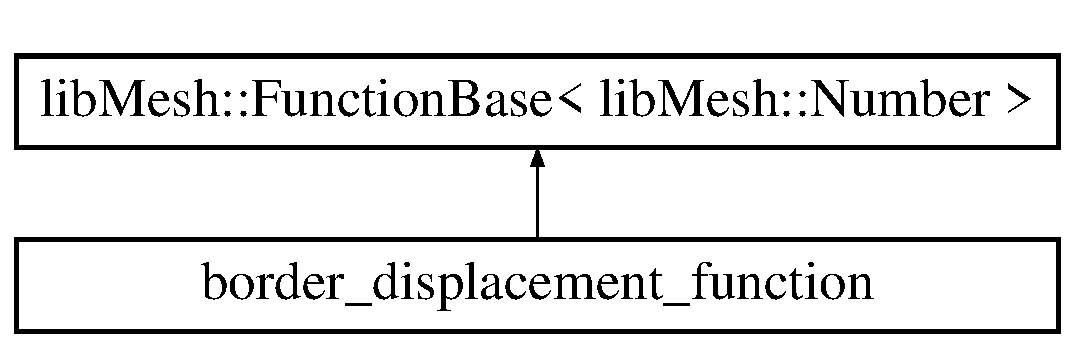
\includegraphics[height=2.000000cm]{classborder__displacement__function}
\end{center}
\end{figure}
\subsection*{Public Member Functions}
\begin{DoxyCompactItemize}
\item 
\hyperlink{classborder__displacement__function_a96fa6052b759f3348654178cab730362}{border\+\_\+displacement\+\_\+function} (unsigned int u\+\_\+var, unsigned int v\+\_\+var, unsigned int w\+\_\+var, lib\+Mesh\+::\+Real x\+\_\+displ=0, lib\+Mesh\+::\+Real y\+\_\+displ=0, lib\+Mesh\+::\+Real z\+\_\+displ=0)
\item 
virtual lib\+Mesh\+::\+Number \hyperlink{classborder__displacement__function_a36164904aab66a842edd7f43cb6b391c}{operator()} (const lib\+Mesh\+::\+Point \&, const lib\+Mesh\+::\+Real=0)
\item 
virtual void \hyperlink{classborder__displacement__function_a286bf7b4ca0e09e3804e2b90730454db}{operator()} (const lib\+Mesh\+::\+Point \&p, const lib\+Mesh\+::\+Real, lib\+Mesh\+::\+Dense\+Vector$<$ lib\+Mesh\+::\+Number $>$ \&output)
\item 
virtual lib\+Mesh\+::\+Unique\+Ptr$<$ Function\+Base$<$ lib\+Mesh\+::\+Number $>$ $>$ \hyperlink{classborder__displacement__function_ae04386c0af6b4722d226c034351d8b5e}{clone} () const 
\end{DoxyCompactItemize}


\subsection{Detailed Description}
3\+D border displacement class, derived from lib\+Mesh\+::\+Function\+Base$<$lib\+Mesh\+::\+Number$>$. 

Definition at line 15 of file common\+\_\+assemble\+\_\+functions\+\_\+elasticity\+\_\+3\+D.\+h.



\subsection{Constructor \& Destructor Documentation}
\hypertarget{classborder__displacement__function_a96fa6052b759f3348654178cab730362}{}\index{border\+\_\+displacement\+\_\+function@{border\+\_\+displacement\+\_\+function}!border\+\_\+displacement\+\_\+function@{border\+\_\+displacement\+\_\+function}}
\index{border\+\_\+displacement\+\_\+function@{border\+\_\+displacement\+\_\+function}!border\+\_\+displacement\+\_\+function@{border\+\_\+displacement\+\_\+function}}
\subsubsection[{border\+\_\+displacement\+\_\+function(unsigned int u\+\_\+var, unsigned int v\+\_\+var, unsigned int w\+\_\+var, lib\+Mesh\+::\+Real x\+\_\+displ=0, lib\+Mesh\+::\+Real y\+\_\+displ=0, lib\+Mesh\+::\+Real z\+\_\+displ=0)}]{\setlength{\rightskip}{0pt plus 5cm}border\+\_\+displacement\+\_\+function\+::border\+\_\+displacement\+\_\+function (
\begin{DoxyParamCaption}
\item[{unsigned int}]{u\+\_\+var, }
\item[{unsigned int}]{v\+\_\+var, }
\item[{unsigned int}]{w\+\_\+var, }
\item[{lib\+Mesh\+::\+Real}]{x\+\_\+displ = {\ttfamily 0}, }
\item[{lib\+Mesh\+::\+Real}]{y\+\_\+displ = {\ttfamily 0}, }
\item[{lib\+Mesh\+::\+Real}]{z\+\_\+displ = {\ttfamily 0}}
\end{DoxyParamCaption}
)\hspace{0.3cm}{\ttfamily [inline]}}\label{classborder__displacement__function_a96fa6052b759f3348654178cab730362}


Definition at line 22 of file common\+\_\+assemble\+\_\+functions\+\_\+elasticity\+\_\+3\+D.\+h.


\begin{DoxyCode}
28                                 : \_u\_var(u\_var),
29                                   \_v\_var(v\_var),
30                                   \_w\_var(w\_var),
31                                   \_x\_displ(x\_displ),
32                                   \_y\_displ(y\_displ),
33                                   \_z\_displ(z\_displ)
34         \{
35             this->\_initialized = \textcolor{keyword}{true};
36         \}
\end{DoxyCode}


\subsection{Member Function Documentation}
\hypertarget{classborder__displacement__function_ae04386c0af6b4722d226c034351d8b5e}{}\index{border\+\_\+displacement\+\_\+function@{border\+\_\+displacement\+\_\+function}!clone@{clone}}
\index{clone@{clone}!border\+\_\+displacement\+\_\+function@{border\+\_\+displacement\+\_\+function}}
\subsubsection[{clone() const }]{\setlength{\rightskip}{0pt plus 5cm}virtual lib\+Mesh\+::\+Unique\+Ptr$<$Function\+Base$<$lib\+Mesh\+::\+Number$>$ $>$ border\+\_\+displacement\+\_\+function\+::clone (
\begin{DoxyParamCaption}
{}
\end{DoxyParamCaption}
) const\hspace{0.3cm}{\ttfamily [inline]}, {\ttfamily [virtual]}}\label{classborder__displacement__function_ae04386c0af6b4722d226c034351d8b5e}


Definition at line 55 of file common\+\_\+assemble\+\_\+functions\+\_\+elasticity\+\_\+3\+D.\+h.


\begin{DoxyCode}
56         \{
57             \textcolor{keywordflow}{return} libMesh::UniquePtr<FunctionBase<libMesh::Number> >
58                 (\textcolor{keyword}{new} \hyperlink{classborder__displacement__function_a96fa6052b759f3348654178cab730362}{border\_displacement\_function}(  \_u\_var, \_v\_var, \_w\_var,
59                                             \_x\_displ, \_y\_displ, \_z\_displ));
60         \}
\end{DoxyCode}
\hypertarget{classborder__displacement__function_a36164904aab66a842edd7f43cb6b391c}{}\index{border\+\_\+displacement\+\_\+function@{border\+\_\+displacement\+\_\+function}!operator()@{operator()}}
\index{operator()@{operator()}!border\+\_\+displacement\+\_\+function@{border\+\_\+displacement\+\_\+function}}
\subsubsection[{operator()(const lib\+Mesh\+::\+Point \&, const lib\+Mesh\+::\+Real=0)}]{\setlength{\rightskip}{0pt plus 5cm}virtual lib\+Mesh\+::\+Number border\+\_\+displacement\+\_\+function\+::operator() (
\begin{DoxyParamCaption}
\item[{const lib\+Mesh\+::\+Point \&}]{, }
\item[{const lib\+Mesh\+::\+Real}]{ = {\ttfamily 0}}
\end{DoxyParamCaption}
)\hspace{0.3cm}{\ttfamily [inline]}, {\ttfamily [virtual]}}\label{classborder__displacement__function_a36164904aab66a842edd7f43cb6b391c}


Definition at line 38 of file common\+\_\+assemble\+\_\+functions\+\_\+elasticity\+\_\+3\+D.\+h.


\begin{DoxyCode}
39         \{
40             libmesh\_not\_implemented();
41         \}
\end{DoxyCode}
\hypertarget{classborder__displacement__function_a286bf7b4ca0e09e3804e2b90730454db}{}\index{border\+\_\+displacement\+\_\+function@{border\+\_\+displacement\+\_\+function}!operator()@{operator()}}
\index{operator()@{operator()}!border\+\_\+displacement\+\_\+function@{border\+\_\+displacement\+\_\+function}}
\subsubsection[{operator()(const lib\+Mesh\+::\+Point \&p, const lib\+Mesh\+::\+Real, lib\+Mesh\+::\+Dense\+Vector$<$ lib\+Mesh\+::\+Number $>$ \&output)}]{\setlength{\rightskip}{0pt plus 5cm}virtual void border\+\_\+displacement\+\_\+function\+::operator() (
\begin{DoxyParamCaption}
\item[{const lib\+Mesh\+::\+Point \&}]{p, }
\item[{const lib\+Mesh\+::\+Real}]{, }
\item[{lib\+Mesh\+::\+Dense\+Vector$<$ lib\+Mesh\+::\+Number $>$ \&}]{output}
\end{DoxyParamCaption}
)\hspace{0.3cm}{\ttfamily [inline]}, {\ttfamily [virtual]}}\label{classborder__displacement__function_a286bf7b4ca0e09e3804e2b90730454db}


Definition at line 43 of file common\+\_\+assemble\+\_\+functions\+\_\+elasticity\+\_\+3\+D.\+h.


\begin{DoxyCode}
46         \{
47             output.resize(3);
48             output.zero();
49 
50             output(\_u\_var) = \_x\_displ;
51             output(\_v\_var) = \_y\_displ;
52             output(\_w\_var) = \_z\_displ;
53         \}
\end{DoxyCode}


The documentation for this class was generated from the following file\+:\begin{DoxyCompactItemize}
\item 
/\+Users/breubreubreu/\+Programming/\+C\+Arl/\+Cpp/src/execs/ext\+\_\+solver\+\_\+libmesh/ext\+\_\+solver\+\_\+libmesh\+\_\+common/include/\hyperlink{common__assemble__functions__elasticity__3_d_8h}{common\+\_\+assemble\+\_\+functions\+\_\+elasticity\+\_\+3\+D.\+h}\end{DoxyCompactItemize}

\hypertarget{structborder__displacement__values}{}\section{border\+\_\+displacement\+\_\+values Struct Reference}
\label{structborder__displacement__values}\index{border\+\_\+displacement\+\_\+values@{border\+\_\+displacement\+\_\+values}}


Small structure with the 3\+D border displacement values.  




{\ttfamily \#include $<$common\+\_\+assemble\+\_\+functions\+\_\+elasticity\+\_\+3\+D.\+h$>$}

\subsection*{Public Attributes}
\begin{DoxyCompactItemize}
\item 
double \hyperlink{structborder__displacement__values_a79fb24700b001a0e4089816f6e9596b1}{x\+\_\+displ}
\item 
double \hyperlink{structborder__displacement__values_add771bac55cf12535ad4329d92c81d92}{y\+\_\+displ}
\item 
double \hyperlink{structborder__displacement__values_a2c7c653e236a44f295db2d74ced8706b}{z\+\_\+displ}
\end{DoxyCompactItemize}


\subsection{Detailed Description}
Small structure with the 3\+D border displacement values. 

Definition at line 64 of file common\+\_\+assemble\+\_\+functions\+\_\+elasticity\+\_\+3\+D.\+h.



\subsection{Member Data Documentation}
\hypertarget{structborder__displacement__values_a79fb24700b001a0e4089816f6e9596b1}{}\index{border\+\_\+displacement\+\_\+values@{border\+\_\+displacement\+\_\+values}!x\+\_\+displ@{x\+\_\+displ}}
\index{x\+\_\+displ@{x\+\_\+displ}!border\+\_\+displacement\+\_\+values@{border\+\_\+displacement\+\_\+values}}
\subsubsection[{x\+\_\+displ}]{\setlength{\rightskip}{0pt plus 5cm}double border\+\_\+displacement\+\_\+values\+::x\+\_\+displ}\label{structborder__displacement__values_a79fb24700b001a0e4089816f6e9596b1}


Definition at line 66 of file common\+\_\+assemble\+\_\+functions\+\_\+elasticity\+\_\+3\+D.\+h.

\hypertarget{structborder__displacement__values_add771bac55cf12535ad4329d92c81d92}{}\index{border\+\_\+displacement\+\_\+values@{border\+\_\+displacement\+\_\+values}!y\+\_\+displ@{y\+\_\+displ}}
\index{y\+\_\+displ@{y\+\_\+displ}!border\+\_\+displacement\+\_\+values@{border\+\_\+displacement\+\_\+values}}
\subsubsection[{y\+\_\+displ}]{\setlength{\rightskip}{0pt plus 5cm}double border\+\_\+displacement\+\_\+values\+::y\+\_\+displ}\label{structborder__displacement__values_add771bac55cf12535ad4329d92c81d92}


Definition at line 67 of file common\+\_\+assemble\+\_\+functions\+\_\+elasticity\+\_\+3\+D.\+h.

\hypertarget{structborder__displacement__values_a2c7c653e236a44f295db2d74ced8706b}{}\index{border\+\_\+displacement\+\_\+values@{border\+\_\+displacement\+\_\+values}!z\+\_\+displ@{z\+\_\+displ}}
\index{z\+\_\+displ@{z\+\_\+displ}!border\+\_\+displacement\+\_\+values@{border\+\_\+displacement\+\_\+values}}
\subsubsection[{z\+\_\+displ}]{\setlength{\rightskip}{0pt plus 5cm}double border\+\_\+displacement\+\_\+values\+::z\+\_\+displ}\label{structborder__displacement__values_a2c7c653e236a44f295db2d74ced8706b}


Definition at line 68 of file common\+\_\+assemble\+\_\+functions\+\_\+elasticity\+\_\+3\+D.\+h.



The documentation for this struct was generated from the following file\+:\begin{DoxyCompactItemize}
\item 
/\+Users/breubreubreu/\+Programming/\+C\+Arl/\+Cpp/src/execs/ext\+\_\+solver\+\_\+libmesh/ext\+\_\+solver\+\_\+libmesh\+\_\+common/include/\hyperlink{common__assemble__functions__elasticity__3_d_8h}{common\+\_\+assemble\+\_\+functions\+\_\+elasticity\+\_\+3\+D.\+h}\end{DoxyCompactItemize}

\hypertarget{structcarl_1_1carl__mult__coupling__input__params}{}\section{carl\+:\+:carl\+\_\+mult\+\_\+coupling\+\_\+input\+\_\+params Struct Reference}
\label{structcarl_1_1carl__mult__coupling__input__params}\index{carl\+::carl\+\_\+mult\+\_\+coupling\+\_\+input\+\_\+params@{carl\+::carl\+\_\+mult\+\_\+coupling\+\_\+input\+\_\+params}}


{\ttfamily \#include $<$carl\+\_\+mult\+\_\+coupling\+\_\+input\+\_\+parser.\+h$>$}

\subsection*{Public Attributes}
\begin{DoxyCompactItemize}
\item 
std\+::string \hyperlink{structcarl_1_1carl__mult__coupling__input__params_a3ad1c5068c4613c3e8b15d64125c4a04}{coupl\+\_\+matrix\+\_\+file}
\begin{DoxyCompactList}\small\item\em Path to the coupling matrix file. \end{DoxyCompactList}\item 
std\+::string \hyperlink{structcarl_1_1carl__mult__coupling__input__params_ad87a4f40746d5fca6085a280adaaa3d0}{input\+\_\+vec\+\_\+file}
\begin{DoxyCompactList}\small\item\em Path to the input vector file. \end{DoxyCompactList}\item 
std\+::string \hyperlink{structcarl_1_1carl__mult__coupling__input__params_ae8b0746e5db705a3ece18ea951b8b9c4}{output\+\_\+base}
\begin{DoxyCompactList}\small\item\em Output filename base. \end{DoxyCompactList}\end{DoxyCompactItemize}


\subsection{Detailed Description}


Definition at line 15 of file carl\+\_\+mult\+\_\+coupling\+\_\+input\+\_\+parser.\+h.



\subsection{Member Data Documentation}
\hypertarget{structcarl_1_1carl__mult__coupling__input__params_a3ad1c5068c4613c3e8b15d64125c4a04}{}\index{carl\+::carl\+\_\+mult\+\_\+coupling\+\_\+input\+\_\+params@{carl\+::carl\+\_\+mult\+\_\+coupling\+\_\+input\+\_\+params}!coupl\+\_\+matrix\+\_\+file@{coupl\+\_\+matrix\+\_\+file}}
\index{coupl\+\_\+matrix\+\_\+file@{coupl\+\_\+matrix\+\_\+file}!carl\+::carl\+\_\+mult\+\_\+coupling\+\_\+input\+\_\+params@{carl\+::carl\+\_\+mult\+\_\+coupling\+\_\+input\+\_\+params}}
\subsubsection[{coupl\+\_\+matrix\+\_\+file}]{\setlength{\rightskip}{0pt plus 5cm}std\+::string carl\+::carl\+\_\+mult\+\_\+coupling\+\_\+input\+\_\+params\+::coupl\+\_\+matrix\+\_\+file}\label{structcarl_1_1carl__mult__coupling__input__params_a3ad1c5068c4613c3e8b15d64125c4a04}


Path to the coupling matrix file. 



Definition at line 16 of file carl\+\_\+mult\+\_\+coupling\+\_\+input\+\_\+parser.\+h.

\hypertarget{structcarl_1_1carl__mult__coupling__input__params_ad87a4f40746d5fca6085a280adaaa3d0}{}\index{carl\+::carl\+\_\+mult\+\_\+coupling\+\_\+input\+\_\+params@{carl\+::carl\+\_\+mult\+\_\+coupling\+\_\+input\+\_\+params}!input\+\_\+vec\+\_\+file@{input\+\_\+vec\+\_\+file}}
\index{input\+\_\+vec\+\_\+file@{input\+\_\+vec\+\_\+file}!carl\+::carl\+\_\+mult\+\_\+coupling\+\_\+input\+\_\+params@{carl\+::carl\+\_\+mult\+\_\+coupling\+\_\+input\+\_\+params}}
\subsubsection[{input\+\_\+vec\+\_\+file}]{\setlength{\rightskip}{0pt plus 5cm}std\+::string carl\+::carl\+\_\+mult\+\_\+coupling\+\_\+input\+\_\+params\+::input\+\_\+vec\+\_\+file}\label{structcarl_1_1carl__mult__coupling__input__params_ad87a4f40746d5fca6085a280adaaa3d0}


Path to the input vector file. 



Definition at line 17 of file carl\+\_\+mult\+\_\+coupling\+\_\+input\+\_\+parser.\+h.

\hypertarget{structcarl_1_1carl__mult__coupling__input__params_ae8b0746e5db705a3ece18ea951b8b9c4}{}\index{carl\+::carl\+\_\+mult\+\_\+coupling\+\_\+input\+\_\+params@{carl\+::carl\+\_\+mult\+\_\+coupling\+\_\+input\+\_\+params}!output\+\_\+base@{output\+\_\+base}}
\index{output\+\_\+base@{output\+\_\+base}!carl\+::carl\+\_\+mult\+\_\+coupling\+\_\+input\+\_\+params@{carl\+::carl\+\_\+mult\+\_\+coupling\+\_\+input\+\_\+params}}
\subsubsection[{output\+\_\+base}]{\setlength{\rightskip}{0pt plus 5cm}std\+::string carl\+::carl\+\_\+mult\+\_\+coupling\+\_\+input\+\_\+params\+::output\+\_\+base}\label{structcarl_1_1carl__mult__coupling__input__params_ae8b0746e5db705a3ece18ea951b8b9c4}


Output filename base. 



Definition at line 18 of file carl\+\_\+mult\+\_\+coupling\+\_\+input\+\_\+parser.\+h.



The documentation for this struct was generated from the following file\+:\begin{DoxyCompactItemize}
\item 
/\+Users/breubreubreu/\+Programming/\+C\+Arl/\+Cpp/src/include/parsers/\hyperlink{carl__mult__coupling__input__parser_8h}{carl\+\_\+mult\+\_\+coupling\+\_\+input\+\_\+parser.\+h}\end{DoxyCompactItemize}

\hypertarget{struct_cell_info}{}\section{Cell\+Info Struct Reference}
\label{struct_cell_info}\index{Cell\+Info@{Cell\+Info}}


{\ttfamily \#include $<$C\+G\+A\+L\+\_\+typedefs.\+h$>$}

\subsection*{Public Attributes}
\begin{DoxyCompactItemize}
\item 
int \hyperlink{struct_cell_info_a23bf3cffc47b6430e60c5263022b684b}{Internal\+Index}
\item 
int \hyperlink{struct_cell_info_a89f6400e5e2bd717aaa615c6ff8e562a}{Ext\+Index}
\item 
int \hyperlink{struct_cell_info_a311c40e7871836b77267349a2c9fadc9}{Ext\+Type}
\item 
std\+::vector$<$ int $>$ \hyperlink{struct_cell_info_a152aa36b31e68fb44de2cbe1192cff3e}{Ext\+Tags}
\item 
int \hyperlink{struct_cell_info_a3e2aef19e88dfd6fd1b9ecdb78e0e425}{Intersection\+Index}
\item 
std\+::vector$<$ int $>$ \hyperlink{struct_cell_info_af5ee3a430a357a5680fed55e446519e3}{face\+Has\+Neighbour}
\item 
bool \hyperlink{struct_cell_info_aa1195689286f14121cad231892aa361e}{To\+Add}
\end{DoxyCompactItemize}


\subsection{Detailed Description}


Definition at line 66 of file C\+G\+A\+L\+\_\+typedefs.\+h.



\subsection{Member Data Documentation}
\hypertarget{struct_cell_info_a89f6400e5e2bd717aaa615c6ff8e562a}{}\index{Cell\+Info@{Cell\+Info}!Ext\+Index@{Ext\+Index}}
\index{Ext\+Index@{Ext\+Index}!Cell\+Info@{Cell\+Info}}
\subsubsection[{Ext\+Index}]{\setlength{\rightskip}{0pt plus 5cm}int Cell\+Info\+::\+Ext\+Index}\label{struct_cell_info_a89f6400e5e2bd717aaa615c6ff8e562a}


Definition at line 69 of file C\+G\+A\+L\+\_\+typedefs.\+h.

\hypertarget{struct_cell_info_a152aa36b31e68fb44de2cbe1192cff3e}{}\index{Cell\+Info@{Cell\+Info}!Ext\+Tags@{Ext\+Tags}}
\index{Ext\+Tags@{Ext\+Tags}!Cell\+Info@{Cell\+Info}}
\subsubsection[{Ext\+Tags}]{\setlength{\rightskip}{0pt plus 5cm}std\+::vector$<$int$>$ Cell\+Info\+::\+Ext\+Tags}\label{struct_cell_info_a152aa36b31e68fb44de2cbe1192cff3e}


Definition at line 71 of file C\+G\+A\+L\+\_\+typedefs.\+h.

\hypertarget{struct_cell_info_a311c40e7871836b77267349a2c9fadc9}{}\index{Cell\+Info@{Cell\+Info}!Ext\+Type@{Ext\+Type}}
\index{Ext\+Type@{Ext\+Type}!Cell\+Info@{Cell\+Info}}
\subsubsection[{Ext\+Type}]{\setlength{\rightskip}{0pt plus 5cm}int Cell\+Info\+::\+Ext\+Type}\label{struct_cell_info_a311c40e7871836b77267349a2c9fadc9}


Definition at line 70 of file C\+G\+A\+L\+\_\+typedefs.\+h.

\hypertarget{struct_cell_info_af5ee3a430a357a5680fed55e446519e3}{}\index{Cell\+Info@{Cell\+Info}!face\+Has\+Neighbour@{face\+Has\+Neighbour}}
\index{face\+Has\+Neighbour@{face\+Has\+Neighbour}!Cell\+Info@{Cell\+Info}}
\subsubsection[{face\+Has\+Neighbour}]{\setlength{\rightskip}{0pt plus 5cm}std\+::vector$<$int$>$ Cell\+Info\+::face\+Has\+Neighbour}\label{struct_cell_info_af5ee3a430a357a5680fed55e446519e3}


Definition at line 73 of file C\+G\+A\+L\+\_\+typedefs.\+h.

\hypertarget{struct_cell_info_a23bf3cffc47b6430e60c5263022b684b}{}\index{Cell\+Info@{Cell\+Info}!Internal\+Index@{Internal\+Index}}
\index{Internal\+Index@{Internal\+Index}!Cell\+Info@{Cell\+Info}}
\subsubsection[{Internal\+Index}]{\setlength{\rightskip}{0pt plus 5cm}int Cell\+Info\+::\+Internal\+Index}\label{struct_cell_info_a23bf3cffc47b6430e60c5263022b684b}


Definition at line 68 of file C\+G\+A\+L\+\_\+typedefs.\+h.

\hypertarget{struct_cell_info_a3e2aef19e88dfd6fd1b9ecdb78e0e425}{}\index{Cell\+Info@{Cell\+Info}!Intersection\+Index@{Intersection\+Index}}
\index{Intersection\+Index@{Intersection\+Index}!Cell\+Info@{Cell\+Info}}
\subsubsection[{Intersection\+Index}]{\setlength{\rightskip}{0pt plus 5cm}int Cell\+Info\+::\+Intersection\+Index}\label{struct_cell_info_a3e2aef19e88dfd6fd1b9ecdb78e0e425}


Definition at line 72 of file C\+G\+A\+L\+\_\+typedefs.\+h.

\hypertarget{struct_cell_info_aa1195689286f14121cad231892aa361e}{}\index{Cell\+Info@{Cell\+Info}!To\+Add@{To\+Add}}
\index{To\+Add@{To\+Add}!Cell\+Info@{Cell\+Info}}
\subsubsection[{To\+Add}]{\setlength{\rightskip}{0pt plus 5cm}bool Cell\+Info\+::\+To\+Add}\label{struct_cell_info_aa1195689286f14121cad231892aa361e}


Definition at line 74 of file C\+G\+A\+L\+\_\+typedefs.\+h.



The documentation for this struct was generated from the following file\+:\begin{DoxyCompactItemize}
\item 
/\+Users/breubreubreu/\+Programming/\+C\+Arl/\+Cpp/src/include/\hyperlink{_c_g_a_l__typedefs_8h}{C\+G\+A\+L\+\_\+typedefs.\+h}\end{DoxyCompactItemize}

\hypertarget{structcarl_1_1coupling__assemble__coupling__input__params}{}\section{carl\+:\+:coupling\+\_\+assemble\+\_\+coupling\+\_\+input\+\_\+params Struct Reference}
\label{structcarl_1_1coupling__assemble__coupling__input__params}\index{carl\+::coupling\+\_\+assemble\+\_\+coupling\+\_\+input\+\_\+params@{carl\+::coupling\+\_\+assemble\+\_\+coupling\+\_\+input\+\_\+params}}


Structure containing the parameters for the construction of the coupling matrices.  




{\ttfamily \#include $<$carl\+\_\+assemble\+\_\+coupling\+\_\+input\+\_\+parser.\+h$>$}

\subsection*{Public Attributes}
\begin{DoxyCompactItemize}
\item 
std\+::string \hyperlink{structcarl_1_1coupling__assemble__coupling__input__params_af311a867cd2103103da6f37851832d18}{mesh\+\_\+\+B\+I\+G\+\_\+file}
\begin{DoxyCompactList}\small\item\em Path to the macro (B\+I\+G) system mesh. \end{DoxyCompactList}\item 
std\+::string \hyperlink{structcarl_1_1coupling__assemble__coupling__input__params_a704cd64a2a6e9c980a46130bc9ec921b}{mesh\+\_\+micro\+\_\+file}
\begin{DoxyCompactList}\small\item\em Path to the micro system mesh. \end{DoxyCompactList}\item 
std\+::string \hyperlink{structcarl_1_1coupling__assemble__coupling__input__params_ad2f08c3035377449238a1d830c666630}{mesh\+\_\+restrict\+\_\+\+B\+I\+G\+\_\+file}
\begin{DoxyCompactList}\small\item\em Path to the restricted macro (B\+I\+G) system mesh. \end{DoxyCompactList}\item 
std\+::string \hyperlink{structcarl_1_1coupling__assemble__coupling__input__params_ab73f9619bf9653bd3ed2cd019dff5f04}{mesh\+\_\+restrict\+\_\+micro\+\_\+file}
\begin{DoxyCompactList}\small\item\em Path to the restricted micro system mesh. \end{DoxyCompactList}\item 
std\+::string \hyperlink{structcarl_1_1coupling__assemble__coupling__input__params_a4fa79c1dc75b71bbda8e54d351ede2d2}{mesh\+\_\+mediator\+\_\+file}
\begin{DoxyCompactList}\small\item\em Path to the mediator system mesh. \end{DoxyCompactList}\item 
std\+::string \hyperlink{structcarl_1_1coupling__assemble__coupling__input__params_aa922a4b0252168abcfd52a9eb3e2b796}{common\+\_\+inter\+\_\+file}
\begin{DoxyCompactList}\small\item\em Common path to the intersection meshes and tables. \end{DoxyCompactList}\item 
std\+::string \hyperlink{structcarl_1_1coupling__assemble__coupling__input__params_a38e203a052eb26245cc22e80084464dd}{equivalence\+\_\+table\+\_\+restrict\+\_\+\+B\+I\+G\+\_\+file}
\begin{DoxyCompactList}\small\item\em Equivalence table between the macro (B\+I\+G) system mesh and its restriction mesh. \end{DoxyCompactList}\item 
std\+::string \hyperlink{structcarl_1_1coupling__assemble__coupling__input__params_a07948e27f6a1a82cffbd1780f28350c7}{equivalence\+\_\+table\+\_\+restrict\+\_\+micro\+\_\+file}
\begin{DoxyCompactList}\small\item\em Equivalence table between the micro system mesh and its restriction mesh. \end{DoxyCompactList}\item 
\hyperlink{namespacecarl_ab4549821791d976a4bb9a3460fe1718e}{carl\+::\+Mediator\+Type} \hyperlink{structcarl_1_1coupling__assemble__coupling__input__params_aa520455b2876272ffc924f060f2a332a}{mediator\+\_\+type}
\begin{DoxyCompactList}\small\item\em Use which mesh as the mediator mesh? {\itshape Values}\+: carl\+::\+Mediator\+Type\+::\+U\+S\+E\+\_\+\+M\+A\+C\+R\+O, carl\+::\+Mediator\+Type\+::\+U\+S\+E\+\_\+\+M\+I\+C\+R\+O or carl\+::\+Mediator\+Type\+::\+U\+S\+E\+\_\+\+E\+X\+T\+E\+R\+N\+A\+L (L\+A\+S\+T C\+A\+S\+E N\+O\+T I\+M\+P\+L\+E\+M\+E\+N\+T\+E\+D Y\+E\+T!). \end{DoxyCompactList}\item 
bool \hyperlink{structcarl_1_1coupling__assemble__coupling__input__params_adefe0489c1e39fb6bb1965a3e80d2bf5}{b\+\_\+\+Use\+Mesh\+\_\+micro\+\_\+\+As\+Mediator}
\begin{DoxyCompactList}\small\item\em Use the micro system\textquotesingle{}s restricted mesh as the mediator? \end{DoxyCompactList}\item 
double \hyperlink{structcarl_1_1coupling__assemble__coupling__input__params_a2cfb03a4663c3c6bc494a88084000249}{coupling\+\_\+width}
\begin{DoxyCompactList}\small\item\em Width of the coupling region. \end{DoxyCompactList}\item 
double \hyperlink{structcarl_1_1coupling__assemble__coupling__input__params_a9f0e82658b0e37c16faed3bc3a176dc1}{coupling\+\_\+rigidity}
\begin{DoxyCompactList}\small\item\em Rigidity used for the coupling matrix. \end{DoxyCompactList}\item 
std\+::string \hyperlink{structcarl_1_1coupling__assemble__coupling__input__params_a1344edd32f644b03b19a499e47fb1ca4}{output\+\_\+folder}
\begin{DoxyCompactList}\small\item\em Path to output folder. \end{DoxyCompactList}\end{DoxyCompactItemize}


\subsection{Detailed Description}
Structure containing the parameters for the construction of the coupling matrices. 

Details on the parameters setup are found in the documentation of \hyperlink{namespacecarl_aba5c04efa5a0abae78d3efd00ae694e3}{carl\+::get\+\_\+assemble\+\_\+coupling\+\_\+input\+\_\+params}(Get\+Pot\& field\+\_\+parser, \hyperlink{structcarl_1_1coupling__assemble__coupling__input__params}{coupling\+\_\+assemble\+\_\+coupling\+\_\+input\+\_\+params}\& input\+\_\+params). 

Definition at line 20 of file carl\+\_\+assemble\+\_\+coupling\+\_\+input\+\_\+parser.\+h.



\subsection{Member Data Documentation}
\hypertarget{structcarl_1_1coupling__assemble__coupling__input__params_adefe0489c1e39fb6bb1965a3e80d2bf5}{}\index{carl\+::coupling\+\_\+assemble\+\_\+coupling\+\_\+input\+\_\+params@{carl\+::coupling\+\_\+assemble\+\_\+coupling\+\_\+input\+\_\+params}!b\+\_\+\+Use\+Mesh\+\_\+micro\+\_\+\+As\+Mediator@{b\+\_\+\+Use\+Mesh\+\_\+micro\+\_\+\+As\+Mediator}}
\index{b\+\_\+\+Use\+Mesh\+\_\+micro\+\_\+\+As\+Mediator@{b\+\_\+\+Use\+Mesh\+\_\+micro\+\_\+\+As\+Mediator}!carl\+::coupling\+\_\+assemble\+\_\+coupling\+\_\+input\+\_\+params@{carl\+::coupling\+\_\+assemble\+\_\+coupling\+\_\+input\+\_\+params}}
\subsubsection[{b\+\_\+\+Use\+Mesh\+\_\+micro\+\_\+\+As\+Mediator}]{\setlength{\rightskip}{0pt plus 5cm}bool carl\+::coupling\+\_\+assemble\+\_\+coupling\+\_\+input\+\_\+params\+::b\+\_\+\+Use\+Mesh\+\_\+micro\+\_\+\+As\+Mediator}\label{structcarl_1_1coupling__assemble__coupling__input__params_adefe0489c1e39fb6bb1965a3e80d2bf5}


Use the micro system\textquotesingle{}s restricted mesh as the mediator? 



Definition at line 36 of file carl\+\_\+assemble\+\_\+coupling\+\_\+input\+\_\+parser.\+h.

\hypertarget{structcarl_1_1coupling__assemble__coupling__input__params_aa922a4b0252168abcfd52a9eb3e2b796}{}\index{carl\+::coupling\+\_\+assemble\+\_\+coupling\+\_\+input\+\_\+params@{carl\+::coupling\+\_\+assemble\+\_\+coupling\+\_\+input\+\_\+params}!common\+\_\+inter\+\_\+file@{common\+\_\+inter\+\_\+file}}
\index{common\+\_\+inter\+\_\+file@{common\+\_\+inter\+\_\+file}!carl\+::coupling\+\_\+assemble\+\_\+coupling\+\_\+input\+\_\+params@{carl\+::coupling\+\_\+assemble\+\_\+coupling\+\_\+input\+\_\+params}}
\subsubsection[{common\+\_\+inter\+\_\+file}]{\setlength{\rightskip}{0pt plus 5cm}std\+::string carl\+::coupling\+\_\+assemble\+\_\+coupling\+\_\+input\+\_\+params\+::common\+\_\+inter\+\_\+file}\label{structcarl_1_1coupling__assemble__coupling__input__params_aa922a4b0252168abcfd52a9eb3e2b796}


Common path to the intersection meshes and tables. 



Definition at line 28 of file carl\+\_\+assemble\+\_\+coupling\+\_\+input\+\_\+parser.\+h.

\hypertarget{structcarl_1_1coupling__assemble__coupling__input__params_a9f0e82658b0e37c16faed3bc3a176dc1}{}\index{carl\+::coupling\+\_\+assemble\+\_\+coupling\+\_\+input\+\_\+params@{carl\+::coupling\+\_\+assemble\+\_\+coupling\+\_\+input\+\_\+params}!coupling\+\_\+rigidity@{coupling\+\_\+rigidity}}
\index{coupling\+\_\+rigidity@{coupling\+\_\+rigidity}!carl\+::coupling\+\_\+assemble\+\_\+coupling\+\_\+input\+\_\+params@{carl\+::coupling\+\_\+assemble\+\_\+coupling\+\_\+input\+\_\+params}}
\subsubsection[{coupling\+\_\+rigidity}]{\setlength{\rightskip}{0pt plus 5cm}double carl\+::coupling\+\_\+assemble\+\_\+coupling\+\_\+input\+\_\+params\+::coupling\+\_\+rigidity}\label{structcarl_1_1coupling__assemble__coupling__input__params_a9f0e82658b0e37c16faed3bc3a176dc1}


Rigidity used for the coupling matrix. 



Definition at line 39 of file carl\+\_\+assemble\+\_\+coupling\+\_\+input\+\_\+parser.\+h.

\hypertarget{structcarl_1_1coupling__assemble__coupling__input__params_a2cfb03a4663c3c6bc494a88084000249}{}\index{carl\+::coupling\+\_\+assemble\+\_\+coupling\+\_\+input\+\_\+params@{carl\+::coupling\+\_\+assemble\+\_\+coupling\+\_\+input\+\_\+params}!coupling\+\_\+width@{coupling\+\_\+width}}
\index{coupling\+\_\+width@{coupling\+\_\+width}!carl\+::coupling\+\_\+assemble\+\_\+coupling\+\_\+input\+\_\+params@{carl\+::coupling\+\_\+assemble\+\_\+coupling\+\_\+input\+\_\+params}}
\subsubsection[{coupling\+\_\+width}]{\setlength{\rightskip}{0pt plus 5cm}double carl\+::coupling\+\_\+assemble\+\_\+coupling\+\_\+input\+\_\+params\+::coupling\+\_\+width}\label{structcarl_1_1coupling__assemble__coupling__input__params_a2cfb03a4663c3c6bc494a88084000249}


Width of the coupling region. 



Definition at line 38 of file carl\+\_\+assemble\+\_\+coupling\+\_\+input\+\_\+parser.\+h.

\hypertarget{structcarl_1_1coupling__assemble__coupling__input__params_a38e203a052eb26245cc22e80084464dd}{}\index{carl\+::coupling\+\_\+assemble\+\_\+coupling\+\_\+input\+\_\+params@{carl\+::coupling\+\_\+assemble\+\_\+coupling\+\_\+input\+\_\+params}!equivalence\+\_\+table\+\_\+restrict\+\_\+\+B\+I\+G\+\_\+file@{equivalence\+\_\+table\+\_\+restrict\+\_\+\+B\+I\+G\+\_\+file}}
\index{equivalence\+\_\+table\+\_\+restrict\+\_\+\+B\+I\+G\+\_\+file@{equivalence\+\_\+table\+\_\+restrict\+\_\+\+B\+I\+G\+\_\+file}!carl\+::coupling\+\_\+assemble\+\_\+coupling\+\_\+input\+\_\+params@{carl\+::coupling\+\_\+assemble\+\_\+coupling\+\_\+input\+\_\+params}}
\subsubsection[{equivalence\+\_\+table\+\_\+restrict\+\_\+\+B\+I\+G\+\_\+file}]{\setlength{\rightskip}{0pt plus 5cm}std\+::string carl\+::coupling\+\_\+assemble\+\_\+coupling\+\_\+input\+\_\+params\+::equivalence\+\_\+table\+\_\+restrict\+\_\+\+B\+I\+G\+\_\+file}\label{structcarl_1_1coupling__assemble__coupling__input__params_a38e203a052eb26245cc22e80084464dd}


Equivalence table between the macro (B\+I\+G) system mesh and its restriction mesh. 



Definition at line 31 of file carl\+\_\+assemble\+\_\+coupling\+\_\+input\+\_\+parser.\+h.

\hypertarget{structcarl_1_1coupling__assemble__coupling__input__params_a07948e27f6a1a82cffbd1780f28350c7}{}\index{carl\+::coupling\+\_\+assemble\+\_\+coupling\+\_\+input\+\_\+params@{carl\+::coupling\+\_\+assemble\+\_\+coupling\+\_\+input\+\_\+params}!equivalence\+\_\+table\+\_\+restrict\+\_\+micro\+\_\+file@{equivalence\+\_\+table\+\_\+restrict\+\_\+micro\+\_\+file}}
\index{equivalence\+\_\+table\+\_\+restrict\+\_\+micro\+\_\+file@{equivalence\+\_\+table\+\_\+restrict\+\_\+micro\+\_\+file}!carl\+::coupling\+\_\+assemble\+\_\+coupling\+\_\+input\+\_\+params@{carl\+::coupling\+\_\+assemble\+\_\+coupling\+\_\+input\+\_\+params}}
\subsubsection[{equivalence\+\_\+table\+\_\+restrict\+\_\+micro\+\_\+file}]{\setlength{\rightskip}{0pt plus 5cm}std\+::string carl\+::coupling\+\_\+assemble\+\_\+coupling\+\_\+input\+\_\+params\+::equivalence\+\_\+table\+\_\+restrict\+\_\+micro\+\_\+file}\label{structcarl_1_1coupling__assemble__coupling__input__params_a07948e27f6a1a82cffbd1780f28350c7}


Equivalence table between the micro system mesh and its restriction mesh. 



Definition at line 33 of file carl\+\_\+assemble\+\_\+coupling\+\_\+input\+\_\+parser.\+h.

\hypertarget{structcarl_1_1coupling__assemble__coupling__input__params_aa520455b2876272ffc924f060f2a332a}{}\index{carl\+::coupling\+\_\+assemble\+\_\+coupling\+\_\+input\+\_\+params@{carl\+::coupling\+\_\+assemble\+\_\+coupling\+\_\+input\+\_\+params}!mediator\+\_\+type@{mediator\+\_\+type}}
\index{mediator\+\_\+type@{mediator\+\_\+type}!carl\+::coupling\+\_\+assemble\+\_\+coupling\+\_\+input\+\_\+params@{carl\+::coupling\+\_\+assemble\+\_\+coupling\+\_\+input\+\_\+params}}
\subsubsection[{mediator\+\_\+type}]{\setlength{\rightskip}{0pt plus 5cm}{\bf carl\+::\+Mediator\+Type} carl\+::coupling\+\_\+assemble\+\_\+coupling\+\_\+input\+\_\+params\+::mediator\+\_\+type}\label{structcarl_1_1coupling__assemble__coupling__input__params_aa520455b2876272ffc924f060f2a332a}


Use which mesh as the mediator mesh? {\itshape Values}\+: carl\+::\+Mediator\+Type\+::\+U\+S\+E\+\_\+\+M\+A\+C\+R\+O, carl\+::\+Mediator\+Type\+::\+U\+S\+E\+\_\+\+M\+I\+C\+R\+O or carl\+::\+Mediator\+Type\+::\+U\+S\+E\+\_\+\+E\+X\+T\+E\+R\+N\+A\+L (L\+A\+S\+T C\+A\+S\+E N\+O\+T I\+M\+P\+L\+E\+M\+E\+N\+T\+E\+D Y\+E\+T!). 



Definition at line 35 of file carl\+\_\+assemble\+\_\+coupling\+\_\+input\+\_\+parser.\+h.

\hypertarget{structcarl_1_1coupling__assemble__coupling__input__params_af311a867cd2103103da6f37851832d18}{}\index{carl\+::coupling\+\_\+assemble\+\_\+coupling\+\_\+input\+\_\+params@{carl\+::coupling\+\_\+assemble\+\_\+coupling\+\_\+input\+\_\+params}!mesh\+\_\+\+B\+I\+G\+\_\+file@{mesh\+\_\+\+B\+I\+G\+\_\+file}}
\index{mesh\+\_\+\+B\+I\+G\+\_\+file@{mesh\+\_\+\+B\+I\+G\+\_\+file}!carl\+::coupling\+\_\+assemble\+\_\+coupling\+\_\+input\+\_\+params@{carl\+::coupling\+\_\+assemble\+\_\+coupling\+\_\+input\+\_\+params}}
\subsubsection[{mesh\+\_\+\+B\+I\+G\+\_\+file}]{\setlength{\rightskip}{0pt plus 5cm}std\+::string carl\+::coupling\+\_\+assemble\+\_\+coupling\+\_\+input\+\_\+params\+::mesh\+\_\+\+B\+I\+G\+\_\+file}\label{structcarl_1_1coupling__assemble__coupling__input__params_af311a867cd2103103da6f37851832d18}


Path to the macro (B\+I\+G) system mesh. 



Definition at line 21 of file carl\+\_\+assemble\+\_\+coupling\+\_\+input\+\_\+parser.\+h.

\hypertarget{structcarl_1_1coupling__assemble__coupling__input__params_a4fa79c1dc75b71bbda8e54d351ede2d2}{}\index{carl\+::coupling\+\_\+assemble\+\_\+coupling\+\_\+input\+\_\+params@{carl\+::coupling\+\_\+assemble\+\_\+coupling\+\_\+input\+\_\+params}!mesh\+\_\+mediator\+\_\+file@{mesh\+\_\+mediator\+\_\+file}}
\index{mesh\+\_\+mediator\+\_\+file@{mesh\+\_\+mediator\+\_\+file}!carl\+::coupling\+\_\+assemble\+\_\+coupling\+\_\+input\+\_\+params@{carl\+::coupling\+\_\+assemble\+\_\+coupling\+\_\+input\+\_\+params}}
\subsubsection[{mesh\+\_\+mediator\+\_\+file}]{\setlength{\rightskip}{0pt plus 5cm}std\+::string carl\+::coupling\+\_\+assemble\+\_\+coupling\+\_\+input\+\_\+params\+::mesh\+\_\+mediator\+\_\+file}\label{structcarl_1_1coupling__assemble__coupling__input__params_a4fa79c1dc75b71bbda8e54d351ede2d2}


Path to the mediator system mesh. 



Definition at line 27 of file carl\+\_\+assemble\+\_\+coupling\+\_\+input\+\_\+parser.\+h.

\hypertarget{structcarl_1_1coupling__assemble__coupling__input__params_a704cd64a2a6e9c980a46130bc9ec921b}{}\index{carl\+::coupling\+\_\+assemble\+\_\+coupling\+\_\+input\+\_\+params@{carl\+::coupling\+\_\+assemble\+\_\+coupling\+\_\+input\+\_\+params}!mesh\+\_\+micro\+\_\+file@{mesh\+\_\+micro\+\_\+file}}
\index{mesh\+\_\+micro\+\_\+file@{mesh\+\_\+micro\+\_\+file}!carl\+::coupling\+\_\+assemble\+\_\+coupling\+\_\+input\+\_\+params@{carl\+::coupling\+\_\+assemble\+\_\+coupling\+\_\+input\+\_\+params}}
\subsubsection[{mesh\+\_\+micro\+\_\+file}]{\setlength{\rightskip}{0pt plus 5cm}std\+::string carl\+::coupling\+\_\+assemble\+\_\+coupling\+\_\+input\+\_\+params\+::mesh\+\_\+micro\+\_\+file}\label{structcarl_1_1coupling__assemble__coupling__input__params_a704cd64a2a6e9c980a46130bc9ec921b}


Path to the micro system mesh. 



Definition at line 22 of file carl\+\_\+assemble\+\_\+coupling\+\_\+input\+\_\+parser.\+h.

\hypertarget{structcarl_1_1coupling__assemble__coupling__input__params_ad2f08c3035377449238a1d830c666630}{}\index{carl\+::coupling\+\_\+assemble\+\_\+coupling\+\_\+input\+\_\+params@{carl\+::coupling\+\_\+assemble\+\_\+coupling\+\_\+input\+\_\+params}!mesh\+\_\+restrict\+\_\+\+B\+I\+G\+\_\+file@{mesh\+\_\+restrict\+\_\+\+B\+I\+G\+\_\+file}}
\index{mesh\+\_\+restrict\+\_\+\+B\+I\+G\+\_\+file@{mesh\+\_\+restrict\+\_\+\+B\+I\+G\+\_\+file}!carl\+::coupling\+\_\+assemble\+\_\+coupling\+\_\+input\+\_\+params@{carl\+::coupling\+\_\+assemble\+\_\+coupling\+\_\+input\+\_\+params}}
\subsubsection[{mesh\+\_\+restrict\+\_\+\+B\+I\+G\+\_\+file}]{\setlength{\rightskip}{0pt plus 5cm}std\+::string carl\+::coupling\+\_\+assemble\+\_\+coupling\+\_\+input\+\_\+params\+::mesh\+\_\+restrict\+\_\+\+B\+I\+G\+\_\+file}\label{structcarl_1_1coupling__assemble__coupling__input__params_ad2f08c3035377449238a1d830c666630}


Path to the restricted macro (B\+I\+G) system mesh. 



Definition at line 24 of file carl\+\_\+assemble\+\_\+coupling\+\_\+input\+\_\+parser.\+h.

\hypertarget{structcarl_1_1coupling__assemble__coupling__input__params_ab73f9619bf9653bd3ed2cd019dff5f04}{}\index{carl\+::coupling\+\_\+assemble\+\_\+coupling\+\_\+input\+\_\+params@{carl\+::coupling\+\_\+assemble\+\_\+coupling\+\_\+input\+\_\+params}!mesh\+\_\+restrict\+\_\+micro\+\_\+file@{mesh\+\_\+restrict\+\_\+micro\+\_\+file}}
\index{mesh\+\_\+restrict\+\_\+micro\+\_\+file@{mesh\+\_\+restrict\+\_\+micro\+\_\+file}!carl\+::coupling\+\_\+assemble\+\_\+coupling\+\_\+input\+\_\+params@{carl\+::coupling\+\_\+assemble\+\_\+coupling\+\_\+input\+\_\+params}}
\subsubsection[{mesh\+\_\+restrict\+\_\+micro\+\_\+file}]{\setlength{\rightskip}{0pt plus 5cm}std\+::string carl\+::coupling\+\_\+assemble\+\_\+coupling\+\_\+input\+\_\+params\+::mesh\+\_\+restrict\+\_\+micro\+\_\+file}\label{structcarl_1_1coupling__assemble__coupling__input__params_ab73f9619bf9653bd3ed2cd019dff5f04}


Path to the restricted micro system mesh. 



Definition at line 25 of file carl\+\_\+assemble\+\_\+coupling\+\_\+input\+\_\+parser.\+h.

\hypertarget{structcarl_1_1coupling__assemble__coupling__input__params_a1344edd32f644b03b19a499e47fb1ca4}{}\index{carl\+::coupling\+\_\+assemble\+\_\+coupling\+\_\+input\+\_\+params@{carl\+::coupling\+\_\+assemble\+\_\+coupling\+\_\+input\+\_\+params}!output\+\_\+folder@{output\+\_\+folder}}
\index{output\+\_\+folder@{output\+\_\+folder}!carl\+::coupling\+\_\+assemble\+\_\+coupling\+\_\+input\+\_\+params@{carl\+::coupling\+\_\+assemble\+\_\+coupling\+\_\+input\+\_\+params}}
\subsubsection[{output\+\_\+folder}]{\setlength{\rightskip}{0pt plus 5cm}std\+::string carl\+::coupling\+\_\+assemble\+\_\+coupling\+\_\+input\+\_\+params\+::output\+\_\+folder}\label{structcarl_1_1coupling__assemble__coupling__input__params_a1344edd32f644b03b19a499e47fb1ca4}


Path to output folder. 



Definition at line 41 of file carl\+\_\+assemble\+\_\+coupling\+\_\+input\+\_\+parser.\+h.



The documentation for this struct was generated from the following file\+:\begin{DoxyCompactItemize}
\item 
/\+Users/breubreubreu/\+Programming/\+C\+Arl/\+Cpp/src/include/parsers/\hyperlink{carl__assemble__coupling__input__parser_8h}{carl\+\_\+assemble\+\_\+coupling\+\_\+input\+\_\+parser.\+h}\end{DoxyCompactItemize}

\hypertarget{classcarl_1_1coupling__matrices__3}{}\section{carl\+:\+:coupling\+\_\+matrices\+\_\+3 Class Reference}
\label{classcarl_1_1coupling__matrices__3}\index{carl\+::coupling\+\_\+matrices\+\_\+3@{carl\+::coupling\+\_\+matrices\+\_\+3}}


{\ttfamily \#include $<$assemble\+\_\+coupling.\+h$>$}

\subsection*{Public Member Functions}
\begin{DoxyCompactItemize}
\item 
\hyperlink{classcarl_1_1coupling__matrices__3_ae0f3ff0a7b313c2905476c153c509fa6}{coupling\+\_\+matrices\+\_\+3} ()
\item 
void \hyperlink{classcarl_1_1coupling__matrices__3_af3bb0a4c9c9cb246d968fb66a054f1c1}{set\+\_\+matrices} (\hyperlink{classcarl_1_1lib_mesh__fe__addresses__3}{lib\+Mesh\+\_\+fe\+\_\+addresses\+\_\+3} \&system\+\_\+type\+\_\+\+A\+A\+A, \hyperlink{classcarl_1_1lib_mesh__fe__addresses__3}{lib\+Mesh\+\_\+fe\+\_\+addresses\+\_\+3} \&system\+\_\+type\+\_\+\+B\+B\+B)
\item 
void \hyperlink{classcarl_1_1coupling__matrices__3_aa7833efcb14dae2535e50228cfc4e766}{build\+\_\+\+L2\+\_\+coupling\+\_\+matrix} (const \hyperlink{classcarl_1_1lib_mesh__fe__addresses__3}{lib\+Mesh\+\_\+fe\+\_\+addresses\+\_\+3} \&system\+\_\+type\+\_\+\+A\+A\+A, const \hyperlink{classcarl_1_1lib_mesh__fe__addresses__3}{lib\+Mesh\+\_\+fe\+\_\+addresses\+\_\+3} \&system\+\_\+type\+\_\+\+B\+B\+B, int qp, const std\+::vector$<$ std\+::vector$<$ lib\+Mesh\+::\+Real $>$ $>$ \&corrected\+\_\+phi\+\_\+\+A\+A\+A, const std\+::vector$<$ std\+::vector$<$ lib\+Mesh\+::\+Real $>$ $>$ \&corrected\+\_\+phi\+\_\+\+B\+B\+B, const std\+::vector$<$ lib\+Mesh\+::\+Real $>$ \&Jx\+W, double L2\+\_\+coupling\+\_\+const)
\item 
void \hyperlink{classcarl_1_1coupling__matrices__3_a0cd97b58bab0b49fa186ffe867bf1b18}{add\+\_\+\+H1\+\_\+coupling\+\_\+matrix} (const \hyperlink{classcarl_1_1lib_mesh__fe__addresses__3}{lib\+Mesh\+\_\+fe\+\_\+addresses\+\_\+3} \&system\+\_\+type\+\_\+\+A\+A\+A, const \hyperlink{classcarl_1_1lib_mesh__fe__addresses__3}{lib\+Mesh\+\_\+fe\+\_\+addresses\+\_\+3} \&system\+\_\+type\+\_\+\+B\+B\+B, int qp, const std\+::vector$<$ std\+::vector$<$ lib\+Mesh\+::\+Real\+Gradient $>$ $>$ \&corrected\+\_\+dphi\+\_\+sys\+A\+A\+A, const std\+::vector$<$ std\+::vector$<$ lib\+Mesh\+::\+Real\+Gradient $>$ $>$ \&corrected\+\_\+dphi\+\_\+sys\+B\+B\+B, const std\+::vector$<$ lib\+Mesh\+::\+Real $>$ \&Jx\+W, const lib\+Mesh\+::\+Number H1\+\_\+coupling\+\_\+const)
\item 
void \hyperlink{classcarl_1_1coupling__matrices__3_a28adf050c759db949c8f0cad8c0e2a7a}{zero} ()
\end{DoxyCompactItemize}
\subsection*{Public Attributes}
\begin{DoxyCompactItemize}
\item 
lib\+Mesh\+::\+Dense\+Matrix$<$ lib\+Mesh\+::\+Number $>$ \hyperlink{classcarl_1_1coupling__matrices__3_a8168867299d675801de227565e969280}{Me}
\item 
lib\+Mesh\+::\+Dense\+Sub\+Matrix$<$ lib\+Mesh\+::\+Number $>$ \hyperlink{classcarl_1_1coupling__matrices__3_a9038b3af932d8a3cbca3662c6a071ff6}{Me\+\_\+uu}
\item 
lib\+Mesh\+::\+Dense\+Sub\+Matrix$<$ lib\+Mesh\+::\+Number $>$ \hyperlink{classcarl_1_1coupling__matrices__3_a4ce35a3abfdcfa68633df7a7f1f685e0}{Me\+\_\+uv}
\item 
lib\+Mesh\+::\+Dense\+Sub\+Matrix$<$ lib\+Mesh\+::\+Number $>$ \hyperlink{classcarl_1_1coupling__matrices__3_a11eb52d03c2c0520f87c75a89ed4d049}{Me\+\_\+uw}
\item 
lib\+Mesh\+::\+Dense\+Sub\+Matrix$<$ lib\+Mesh\+::\+Number $>$ \hyperlink{classcarl_1_1coupling__matrices__3_a7f606b964255ab6db7df26647ca7676c}{Me\+\_\+vu}
\item 
lib\+Mesh\+::\+Dense\+Sub\+Matrix$<$ lib\+Mesh\+::\+Number $>$ \hyperlink{classcarl_1_1coupling__matrices__3_af53f357fe4ae7938cefda80a92900bef}{Me\+\_\+vv}
\item 
lib\+Mesh\+::\+Dense\+Sub\+Matrix$<$ lib\+Mesh\+::\+Number $>$ \hyperlink{classcarl_1_1coupling__matrices__3_a384c93a0e2bfe69a4b908b333e226113}{Me\+\_\+vw}
\item 
lib\+Mesh\+::\+Dense\+Sub\+Matrix$<$ lib\+Mesh\+::\+Number $>$ \hyperlink{classcarl_1_1coupling__matrices__3_a3f3132dbd7587e504d12c047c598bc52}{Me\+\_\+wu}
\item 
lib\+Mesh\+::\+Dense\+Sub\+Matrix$<$ lib\+Mesh\+::\+Number $>$ \hyperlink{classcarl_1_1coupling__matrices__3_a34a3d938e7ad54997b5d8a227614f983}{Me\+\_\+wv}
\item 
lib\+Mesh\+::\+Dense\+Sub\+Matrix$<$ lib\+Mesh\+::\+Number $>$ \hyperlink{classcarl_1_1coupling__matrices__3_a9b360e5c33276d238262dfe40aaa4aeb}{Me\+\_\+ww}
\end{DoxyCompactItemize}


\subsection{Detailed Description}


Definition at line 93 of file assemble\+\_\+coupling.\+h.



\subsection{Constructor \& Destructor Documentation}
\hypertarget{classcarl_1_1coupling__matrices__3_ae0f3ff0a7b313c2905476c153c509fa6}{}\index{carl\+::coupling\+\_\+matrices\+\_\+3@{carl\+::coupling\+\_\+matrices\+\_\+3}!coupling\+\_\+matrices\+\_\+3@{coupling\+\_\+matrices\+\_\+3}}
\index{coupling\+\_\+matrices\+\_\+3@{coupling\+\_\+matrices\+\_\+3}!carl\+::coupling\+\_\+matrices\+\_\+3@{carl\+::coupling\+\_\+matrices\+\_\+3}}
\subsubsection[{coupling\+\_\+matrices\+\_\+3()}]{\setlength{\rightskip}{0pt plus 5cm}carl\+::coupling\+\_\+matrices\+\_\+3\+::coupling\+\_\+matrices\+\_\+3 (
\begin{DoxyParamCaption}
{}
\end{DoxyParamCaption}
)\hspace{0.3cm}{\ttfamily [inline]}}\label{classcarl_1_1coupling__matrices__3_ae0f3ff0a7b313c2905476c153c509fa6}


Definition at line 100 of file assemble\+\_\+coupling.\+h.


\begin{DoxyCode}
100                           :
101             \hyperlink{classcarl_1_1coupling__matrices__3_a9038b3af932d8a3cbca3662c6a071ff6}{Me\_uu}
102             \{ \hyperlink{classcarl_1_1coupling__matrices__3_a8168867299d675801de227565e969280}{Me} \}, \hyperlink{classcarl_1_1coupling__matrices__3_a4ce35a3abfdcfa68633df7a7f1f685e0}{Me\_uv}
103             \{ \hyperlink{classcarl_1_1coupling__matrices__3_a8168867299d675801de227565e969280}{Me} \}, \hyperlink{classcarl_1_1coupling__matrices__3_a11eb52d03c2c0520f87c75a89ed4d049}{Me\_uw}
104             \{ \hyperlink{classcarl_1_1coupling__matrices__3_a8168867299d675801de227565e969280}{Me} \}, \hyperlink{classcarl_1_1coupling__matrices__3_a7f606b964255ab6db7df26647ca7676c}{Me\_vu}
105             \{ \hyperlink{classcarl_1_1coupling__matrices__3_a8168867299d675801de227565e969280}{Me} \}, \hyperlink{classcarl_1_1coupling__matrices__3_af53f357fe4ae7938cefda80a92900bef}{Me\_vv}
106             \{ \hyperlink{classcarl_1_1coupling__matrices__3_a8168867299d675801de227565e969280}{Me} \}, \hyperlink{classcarl_1_1coupling__matrices__3_a384c93a0e2bfe69a4b908b333e226113}{Me\_vw}
107             \{ \hyperlink{classcarl_1_1coupling__matrices__3_a8168867299d675801de227565e969280}{Me} \}, \hyperlink{classcarl_1_1coupling__matrices__3_a3f3132dbd7587e504d12c047c598bc52}{Me\_wu}
108             \{ \hyperlink{classcarl_1_1coupling__matrices__3_a8168867299d675801de227565e969280}{Me} \}, \hyperlink{classcarl_1_1coupling__matrices__3_a34a3d938e7ad54997b5d8a227614f983}{Me\_wv}
109             \{ \hyperlink{classcarl_1_1coupling__matrices__3_a8168867299d675801de227565e969280}{Me} \}, \hyperlink{classcarl_1_1coupling__matrices__3_a9b360e5c33276d238262dfe40aaa4aeb}{Me\_ww}
110             \{ \hyperlink{classcarl_1_1coupling__matrices__3_a8168867299d675801de227565e969280}{Me} \}
111     \{
112 
113     \}
\end{DoxyCode}


\subsection{Member Function Documentation}
\hypertarget{classcarl_1_1coupling__matrices__3_a0cd97b58bab0b49fa186ffe867bf1b18}{}\index{carl\+::coupling\+\_\+matrices\+\_\+3@{carl\+::coupling\+\_\+matrices\+\_\+3}!add\+\_\+\+H1\+\_\+coupling\+\_\+matrix@{add\+\_\+\+H1\+\_\+coupling\+\_\+matrix}}
\index{add\+\_\+\+H1\+\_\+coupling\+\_\+matrix@{add\+\_\+\+H1\+\_\+coupling\+\_\+matrix}!carl\+::coupling\+\_\+matrices\+\_\+3@{carl\+::coupling\+\_\+matrices\+\_\+3}}
\subsubsection[{add\+\_\+\+H1\+\_\+coupling\+\_\+matrix(const lib\+Mesh\+\_\+fe\+\_\+addresses\+\_\+3 \&system\+\_\+type\+\_\+\+A\+A\+A, const lib\+Mesh\+\_\+fe\+\_\+addresses\+\_\+3 \&system\+\_\+type\+\_\+\+B\+B\+B, int qp, const std\+::vector$<$ std\+::vector$<$ lib\+Mesh\+::\+Real\+Gradient $>$ $>$ \&corrected\+\_\+dphi\+\_\+sys\+A\+A\+A, const std\+::vector$<$ std\+::vector$<$ lib\+Mesh\+::\+Real\+Gradient $>$ $>$ \&corrected\+\_\+dphi\+\_\+sys\+B\+B\+B, const std\+::vector$<$ lib\+Mesh\+::\+Real $>$ \&\+Jx\+W, const lib\+Mesh\+::\+Number H1\+\_\+coupling\+\_\+const)}]{\setlength{\rightskip}{0pt plus 5cm}void carl\+::coupling\+\_\+matrices\+\_\+3\+::add\+\_\+\+H1\+\_\+coupling\+\_\+matrix (
\begin{DoxyParamCaption}
\item[{const {\bf lib\+Mesh\+\_\+fe\+\_\+addresses\+\_\+3} \&}]{system\+\_\+type\+\_\+\+A\+A\+A, }
\item[{const {\bf lib\+Mesh\+\_\+fe\+\_\+addresses\+\_\+3} \&}]{system\+\_\+type\+\_\+\+B\+B\+B, }
\item[{int}]{qp, }
\item[{const std\+::vector$<$ std\+::vector$<$ lib\+Mesh\+::\+Real\+Gradient $>$ $>$ \&}]{corrected\+\_\+dphi\+\_\+sys\+A\+A\+A, }
\item[{const std\+::vector$<$ std\+::vector$<$ lib\+Mesh\+::\+Real\+Gradient $>$ $>$ \&}]{corrected\+\_\+dphi\+\_\+sys\+B\+B\+B, }
\item[{const std\+::vector$<$ lib\+Mesh\+::\+Real $>$ \&}]{Jx\+W, }
\item[{const lib\+Mesh\+::\+Number}]{H1\+\_\+coupling\+\_\+const}
\end{DoxyParamCaption}
)\hspace{0.3cm}{\ttfamily [inline]}}\label{classcarl_1_1coupling__matrices__3_a0cd97b58bab0b49fa186ffe867bf1b18}


Definition at line 176 of file assemble\+\_\+coupling.\+h.


\begin{DoxyCode}
182     \{
183         \textcolor{keywordtype}{unsigned} \textcolor{keywordtype}{int} n\_components = 3;
184         \hyperlink{weak__formulations_8cpp_a9fcc3dd62b4a38808d4cfdae87d771e4}{H1\_Coupling\_Extra\_Term}(\hyperlink{classcarl_1_1coupling__matrices__3_a9038b3af932d8a3cbca3662c6a071ff6}{Me\_uu}, qp, system\_type\_AAA.u\_var,
185                 system\_type\_BBB.u\_var, n\_components, n\_components,
186                 corrected\_dphi\_sysAAA, corrected\_dphi\_sysBBB,
187                 system\_type\_AAA.n\_dofs\_u, system\_type\_BBB.n\_dofs\_u, JxW,
188                 H1\_coupling\_const);
189 
190         \hyperlink{weak__formulations_8cpp_a9fcc3dd62b4a38808d4cfdae87d771e4}{H1\_Coupling\_Extra\_Term}(\hyperlink{classcarl_1_1coupling__matrices__3_a4ce35a3abfdcfa68633df7a7f1f685e0}{Me\_uv}, qp, system\_type\_AAA.u\_var,
191                 system\_type\_BBB.v\_var, n\_components, n\_components,
192                 corrected\_dphi\_sysAAA, corrected\_dphi\_sysBBB,
193                 system\_type\_AAA.n\_dofs\_u, system\_type\_BBB.n\_dofs\_v, JxW,
194                 H1\_coupling\_const);
195 
196         \hyperlink{weak__formulations_8cpp_a9fcc3dd62b4a38808d4cfdae87d771e4}{H1\_Coupling\_Extra\_Term}(\hyperlink{classcarl_1_1coupling__matrices__3_a11eb52d03c2c0520f87c75a89ed4d049}{Me\_uw}, qp, system\_type\_AAA.u\_var,
197                 system\_type\_BBB.w\_var, n\_components, n\_components,
198                 corrected\_dphi\_sysAAA, corrected\_dphi\_sysBBB,
199                 system\_type\_AAA.n\_dofs\_u, system\_type\_BBB.n\_dofs\_w, JxW,
200                 H1\_coupling\_const);
201 
202         \hyperlink{weak__formulations_8cpp_a9fcc3dd62b4a38808d4cfdae87d771e4}{H1\_Coupling\_Extra\_Term}(\hyperlink{classcarl_1_1coupling__matrices__3_a7f606b964255ab6db7df26647ca7676c}{Me\_vu}, qp, system\_type\_AAA.v\_var,
203                 system\_type\_BBB.u\_var, n\_components, n\_components,
204                 corrected\_dphi\_sysAAA, corrected\_dphi\_sysBBB,
205                 system\_type\_AAA.n\_dofs\_v, system\_type\_BBB.n\_dofs\_u, JxW,
206                 H1\_coupling\_const);
207 
208         \hyperlink{weak__formulations_8cpp_a9fcc3dd62b4a38808d4cfdae87d771e4}{H1\_Coupling\_Extra\_Term}(\hyperlink{classcarl_1_1coupling__matrices__3_af53f357fe4ae7938cefda80a92900bef}{Me\_vv}, qp, system\_type\_AAA.v\_var,
209                 system\_type\_BBB.v\_var, n\_components, n\_components,
210                 corrected\_dphi\_sysAAA, corrected\_dphi\_sysBBB,
211                 system\_type\_AAA.n\_dofs\_v, system\_type\_BBB.n\_dofs\_v, JxW,
212                 H1\_coupling\_const);
213 
214         \hyperlink{weak__formulations_8cpp_a9fcc3dd62b4a38808d4cfdae87d771e4}{H1\_Coupling\_Extra\_Term}(\hyperlink{classcarl_1_1coupling__matrices__3_a384c93a0e2bfe69a4b908b333e226113}{Me\_vw}, qp, system\_type\_AAA.v\_var,
215                 system\_type\_BBB.w\_var, n\_components, n\_components,
216                 corrected\_dphi\_sysAAA, corrected\_dphi\_sysBBB,
217                 system\_type\_AAA.n\_dofs\_v, system\_type\_BBB.n\_dofs\_w, JxW,
218                 H1\_coupling\_const);
219 
220         \hyperlink{weak__formulations_8cpp_a9fcc3dd62b4a38808d4cfdae87d771e4}{H1\_Coupling\_Extra\_Term}(\hyperlink{classcarl_1_1coupling__matrices__3_a3f3132dbd7587e504d12c047c598bc52}{Me\_wu}, qp, system\_type\_AAA.w\_var,
221                 system\_type\_BBB.u\_var, n\_components, n\_components,
222                 corrected\_dphi\_sysAAA, corrected\_dphi\_sysBBB,
223                 system\_type\_AAA.n\_dofs\_w, system\_type\_BBB.n\_dofs\_u, JxW,
224                 H1\_coupling\_const);
225 
226         \hyperlink{weak__formulations_8cpp_a9fcc3dd62b4a38808d4cfdae87d771e4}{H1\_Coupling\_Extra\_Term}(\hyperlink{classcarl_1_1coupling__matrices__3_a34a3d938e7ad54997b5d8a227614f983}{Me\_wv}, qp, system\_type\_AAA.w\_var,
227                 system\_type\_BBB.v\_var, n\_components, n\_components,
228                 corrected\_dphi\_sysAAA, corrected\_dphi\_sysBBB,
229                 system\_type\_AAA.n\_dofs\_w, system\_type\_BBB.n\_dofs\_v, JxW,
230                 H1\_coupling\_const);
231 
232         \hyperlink{weak__formulations_8cpp_a9fcc3dd62b4a38808d4cfdae87d771e4}{H1\_Coupling\_Extra\_Term}(\hyperlink{classcarl_1_1coupling__matrices__3_a9b360e5c33276d238262dfe40aaa4aeb}{Me\_ww}, qp, system\_type\_AAA.w\_var,
233                 system\_type\_BBB.w\_var, n\_components, n\_components,
234                 corrected\_dphi\_sysAAA, corrected\_dphi\_sysBBB,
235                 system\_type\_AAA.n\_dofs\_w, system\_type\_BBB.n\_dofs\_w, JxW,
236                 H1\_coupling\_const);
237     \}
\end{DoxyCode}
\hypertarget{classcarl_1_1coupling__matrices__3_aa7833efcb14dae2535e50228cfc4e766}{}\index{carl\+::coupling\+\_\+matrices\+\_\+3@{carl\+::coupling\+\_\+matrices\+\_\+3}!build\+\_\+\+L2\+\_\+coupling\+\_\+matrix@{build\+\_\+\+L2\+\_\+coupling\+\_\+matrix}}
\index{build\+\_\+\+L2\+\_\+coupling\+\_\+matrix@{build\+\_\+\+L2\+\_\+coupling\+\_\+matrix}!carl\+::coupling\+\_\+matrices\+\_\+3@{carl\+::coupling\+\_\+matrices\+\_\+3}}
\subsubsection[{build\+\_\+\+L2\+\_\+coupling\+\_\+matrix(const lib\+Mesh\+\_\+fe\+\_\+addresses\+\_\+3 \&system\+\_\+type\+\_\+\+A\+A\+A, const lib\+Mesh\+\_\+fe\+\_\+addresses\+\_\+3 \&system\+\_\+type\+\_\+\+B\+B\+B, int qp, const std\+::vector$<$ std\+::vector$<$ lib\+Mesh\+::\+Real $>$ $>$ \&corrected\+\_\+phi\+\_\+\+A\+A\+A, const std\+::vector$<$ std\+::vector$<$ lib\+Mesh\+::\+Real $>$ $>$ \&corrected\+\_\+phi\+\_\+\+B\+B\+B, const std\+::vector$<$ lib\+Mesh\+::\+Real $>$ \&\+Jx\+W, double L2\+\_\+coupling\+\_\+const)}]{\setlength{\rightskip}{0pt plus 5cm}void carl\+::coupling\+\_\+matrices\+\_\+3\+::build\+\_\+\+L2\+\_\+coupling\+\_\+matrix (
\begin{DoxyParamCaption}
\item[{const {\bf lib\+Mesh\+\_\+fe\+\_\+addresses\+\_\+3} \&}]{system\+\_\+type\+\_\+\+A\+A\+A, }
\item[{const {\bf lib\+Mesh\+\_\+fe\+\_\+addresses\+\_\+3} \&}]{system\+\_\+type\+\_\+\+B\+B\+B, }
\item[{int}]{qp, }
\item[{const std\+::vector$<$ std\+::vector$<$ lib\+Mesh\+::\+Real $>$ $>$ \&}]{corrected\+\_\+phi\+\_\+\+A\+A\+A, }
\item[{const std\+::vector$<$ std\+::vector$<$ lib\+Mesh\+::\+Real $>$ $>$ \&}]{corrected\+\_\+phi\+\_\+\+B\+B\+B, }
\item[{const std\+::vector$<$ lib\+Mesh\+::\+Real $>$ \&}]{Jx\+W, }
\item[{double}]{L2\+\_\+coupling\+\_\+const}
\end{DoxyParamCaption}
)\hspace{0.3cm}{\ttfamily [inline]}}\label{classcarl_1_1coupling__matrices__3_aa7833efcb14dae2535e50228cfc4e766}


Definition at line 157 of file assemble\+\_\+coupling.\+h.


\begin{DoxyCode}
162     \{
163         \hyperlink{weak__formulations_8cpp_a07058f23d211d05b82733ac08fc74baa}{L2\_Coupling}(\hyperlink{classcarl_1_1coupling__matrices__3_a9038b3af932d8a3cbca3662c6a071ff6}{Me\_uu}, qp, corrected\_phi\_AAA, corrected\_phi\_BBB,
164                 system\_type\_AAA.n\_dofs\_u, system\_type\_BBB.n\_dofs\_u, JxW,
165                 L2\_coupling\_const);
166 
167         \hyperlink{weak__formulations_8cpp_a07058f23d211d05b82733ac08fc74baa}{L2\_Coupling}(\hyperlink{classcarl_1_1coupling__matrices__3_af53f357fe4ae7938cefda80a92900bef}{Me\_vv}, qp, corrected\_phi\_AAA, corrected\_phi\_BBB,
168                 system\_type\_AAA.n\_dofs\_v, system\_type\_BBB.n\_dofs\_v, JxW,
169                 L2\_coupling\_const);
170 
171         \hyperlink{weak__formulations_8cpp_a07058f23d211d05b82733ac08fc74baa}{L2\_Coupling}(\hyperlink{classcarl_1_1coupling__matrices__3_a9b360e5c33276d238262dfe40aaa4aeb}{Me\_ww}, qp, corrected\_phi\_AAA, corrected\_phi\_BBB,
172                 system\_type\_AAA.n\_dofs\_w, system\_type\_BBB.n\_dofs\_w, JxW,
173                 L2\_coupling\_const);
174     \}
\end{DoxyCode}
\hypertarget{classcarl_1_1coupling__matrices__3_af3bb0a4c9c9cb246d968fb66a054f1c1}{}\index{carl\+::coupling\+\_\+matrices\+\_\+3@{carl\+::coupling\+\_\+matrices\+\_\+3}!set\+\_\+matrices@{set\+\_\+matrices}}
\index{set\+\_\+matrices@{set\+\_\+matrices}!carl\+::coupling\+\_\+matrices\+\_\+3@{carl\+::coupling\+\_\+matrices\+\_\+3}}
\subsubsection[{set\+\_\+matrices(lib\+Mesh\+\_\+fe\+\_\+addresses\+\_\+3 \&system\+\_\+type\+\_\+\+A\+A\+A, lib\+Mesh\+\_\+fe\+\_\+addresses\+\_\+3 \&system\+\_\+type\+\_\+\+B\+B\+B)}]{\setlength{\rightskip}{0pt plus 5cm}void carl\+::coupling\+\_\+matrices\+\_\+3\+::set\+\_\+matrices (
\begin{DoxyParamCaption}
\item[{{\bf lib\+Mesh\+\_\+fe\+\_\+addresses\+\_\+3} \&}]{system\+\_\+type\+\_\+\+A\+A\+A, }
\item[{{\bf lib\+Mesh\+\_\+fe\+\_\+addresses\+\_\+3} \&}]{system\+\_\+type\+\_\+\+B\+B\+B}
\end{DoxyParamCaption}
)\hspace{0.3cm}{\ttfamily [inline]}}\label{classcarl_1_1coupling__matrices__3_af3bb0a4c9c9cb246d968fb66a054f1c1}


Definition at line 115 of file assemble\+\_\+coupling.\+h.


\begin{DoxyCode}
117     \{
118         \hyperlink{classcarl_1_1coupling__matrices__3_a8168867299d675801de227565e969280}{Me}.resize(system\_type\_AAA.n\_dofs, system\_type\_BBB.n\_dofs);
119 
120         \hyperlink{classcarl_1_1coupling__matrices__3_a9038b3af932d8a3cbca3662c6a071ff6}{Me\_uu}.reposition(system\_type\_AAA.u\_var * system\_type\_AAA.n\_dofs\_u,
121                 system\_type\_BBB.u\_var * system\_type\_BBB.n\_dofs\_u,
122                 system\_type\_AAA.n\_dofs\_u, system\_type\_BBB.n\_dofs\_u);
123 
124         \hyperlink{classcarl_1_1coupling__matrices__3_a4ce35a3abfdcfa68633df7a7f1f685e0}{Me\_uv}.reposition(system\_type\_AAA.u\_var * system\_type\_AAA.n\_dofs\_u,
125                 system\_type\_BBB.v\_var * system\_type\_BBB.n\_dofs\_v,
126                 system\_type\_AAA.n\_dofs\_u, system\_type\_BBB.n\_dofs\_v);
127 
128         \hyperlink{classcarl_1_1coupling__matrices__3_a11eb52d03c2c0520f87c75a89ed4d049}{Me\_uw}.reposition(system\_type\_AAA.u\_var * system\_type\_AAA.n\_dofs\_u,
129                 system\_type\_BBB.w\_var * system\_type\_BBB.n\_dofs\_w,
130                 system\_type\_AAA.n\_dofs\_u, system\_type\_BBB.n\_dofs\_w);
131 
132         \hyperlink{classcarl_1_1coupling__matrices__3_a7f606b964255ab6db7df26647ca7676c}{Me\_vu}.reposition(system\_type\_AAA.v\_var * system\_type\_AAA.n\_dofs\_v,
133                 system\_type\_BBB.u\_var * system\_type\_BBB.n\_dofs\_u,
134                 system\_type\_AAA.n\_dofs\_v, system\_type\_BBB.n\_dofs\_u);
135 
136         \hyperlink{classcarl_1_1coupling__matrices__3_af53f357fe4ae7938cefda80a92900bef}{Me\_vv}.reposition(system\_type\_AAA.v\_var * system\_type\_AAA.n\_dofs\_v,
137                 system\_type\_BBB.v\_var * system\_type\_BBB.n\_dofs\_v,
138                 system\_type\_AAA.n\_dofs\_v, system\_type\_BBB.n\_dofs\_v);
139 
140         \hyperlink{classcarl_1_1coupling__matrices__3_a384c93a0e2bfe69a4b908b333e226113}{Me\_vw}.reposition(system\_type\_AAA.v\_var * system\_type\_AAA.n\_dofs\_v,
141                 system\_type\_BBB.w\_var * system\_type\_BBB.n\_dofs\_w,
142                 system\_type\_AAA.n\_dofs\_v, system\_type\_BBB.n\_dofs\_w);
143 
144         \hyperlink{classcarl_1_1coupling__matrices__3_a3f3132dbd7587e504d12c047c598bc52}{Me\_wu}.reposition(system\_type\_AAA.w\_var * system\_type\_AAA.n\_dofs\_w,
145                 system\_type\_BBB.u\_var * system\_type\_BBB.n\_dofs\_u,
146                 system\_type\_AAA.n\_dofs\_w, system\_type\_BBB.n\_dofs\_u);
147 
148         \hyperlink{classcarl_1_1coupling__matrices__3_a34a3d938e7ad54997b5d8a227614f983}{Me\_wv}.reposition(system\_type\_AAA.w\_var * system\_type\_AAA.n\_dofs\_w,
149                 system\_type\_BBB.v\_var * system\_type\_BBB.n\_dofs\_v,
150                 system\_type\_AAA.n\_dofs\_w, system\_type\_BBB.n\_dofs\_v);
151 
152         \hyperlink{classcarl_1_1coupling__matrices__3_a9b360e5c33276d238262dfe40aaa4aeb}{Me\_ww}.reposition(system\_type\_AAA.w\_var * system\_type\_AAA.n\_dofs\_w,
153                 system\_type\_BBB.w\_var * system\_type\_BBB.n\_dofs\_w,
154                 system\_type\_AAA.n\_dofs\_w, system\_type\_BBB.n\_dofs\_w);
155     \}
\end{DoxyCode}
\hypertarget{classcarl_1_1coupling__matrices__3_a28adf050c759db949c8f0cad8c0e2a7a}{}\index{carl\+::coupling\+\_\+matrices\+\_\+3@{carl\+::coupling\+\_\+matrices\+\_\+3}!zero@{zero}}
\index{zero@{zero}!carl\+::coupling\+\_\+matrices\+\_\+3@{carl\+::coupling\+\_\+matrices\+\_\+3}}
\subsubsection[{zero()}]{\setlength{\rightskip}{0pt plus 5cm}void carl\+::coupling\+\_\+matrices\+\_\+3\+::zero (
\begin{DoxyParamCaption}
{}
\end{DoxyParamCaption}
)\hspace{0.3cm}{\ttfamily [inline]}}\label{classcarl_1_1coupling__matrices__3_a28adf050c759db949c8f0cad8c0e2a7a}


Definition at line 240 of file assemble\+\_\+coupling.\+h.


\begin{DoxyCode}
241     \{
242         \hyperlink{classcarl_1_1coupling__matrices__3_a8168867299d675801de227565e969280}{Me}.zero();
243     \}
\end{DoxyCode}


\subsection{Member Data Documentation}
\hypertarget{classcarl_1_1coupling__matrices__3_a8168867299d675801de227565e969280}{}\index{carl\+::coupling\+\_\+matrices\+\_\+3@{carl\+::coupling\+\_\+matrices\+\_\+3}!Me@{Me}}
\index{Me@{Me}!carl\+::coupling\+\_\+matrices\+\_\+3@{carl\+::coupling\+\_\+matrices\+\_\+3}}
\subsubsection[{Me}]{\setlength{\rightskip}{0pt plus 5cm}lib\+Mesh\+::\+Dense\+Matrix$<$lib\+Mesh\+::\+Number$>$ carl\+::coupling\+\_\+matrices\+\_\+3\+::\+Me}\label{classcarl_1_1coupling__matrices__3_a8168867299d675801de227565e969280}


Definition at line 96 of file assemble\+\_\+coupling.\+h.

\hypertarget{classcarl_1_1coupling__matrices__3_a9038b3af932d8a3cbca3662c6a071ff6}{}\index{carl\+::coupling\+\_\+matrices\+\_\+3@{carl\+::coupling\+\_\+matrices\+\_\+3}!Me\+\_\+uu@{Me\+\_\+uu}}
\index{Me\+\_\+uu@{Me\+\_\+uu}!carl\+::coupling\+\_\+matrices\+\_\+3@{carl\+::coupling\+\_\+matrices\+\_\+3}}
\subsubsection[{Me\+\_\+uu}]{\setlength{\rightskip}{0pt plus 5cm}lib\+Mesh\+::\+Dense\+Sub\+Matrix$<$lib\+Mesh\+::\+Number$>$ carl\+::coupling\+\_\+matrices\+\_\+3\+::\+Me\+\_\+uu}\label{classcarl_1_1coupling__matrices__3_a9038b3af932d8a3cbca3662c6a071ff6}


Definition at line 97 of file assemble\+\_\+coupling.\+h.

\hypertarget{classcarl_1_1coupling__matrices__3_a4ce35a3abfdcfa68633df7a7f1f685e0}{}\index{carl\+::coupling\+\_\+matrices\+\_\+3@{carl\+::coupling\+\_\+matrices\+\_\+3}!Me\+\_\+uv@{Me\+\_\+uv}}
\index{Me\+\_\+uv@{Me\+\_\+uv}!carl\+::coupling\+\_\+matrices\+\_\+3@{carl\+::coupling\+\_\+matrices\+\_\+3}}
\subsubsection[{Me\+\_\+uv}]{\setlength{\rightskip}{0pt plus 5cm}lib\+Mesh\+::\+Dense\+Sub\+Matrix$<$lib\+Mesh\+::\+Number$>$ carl\+::coupling\+\_\+matrices\+\_\+3\+::\+Me\+\_\+uv}\label{classcarl_1_1coupling__matrices__3_a4ce35a3abfdcfa68633df7a7f1f685e0}


Definition at line 97 of file assemble\+\_\+coupling.\+h.

\hypertarget{classcarl_1_1coupling__matrices__3_a11eb52d03c2c0520f87c75a89ed4d049}{}\index{carl\+::coupling\+\_\+matrices\+\_\+3@{carl\+::coupling\+\_\+matrices\+\_\+3}!Me\+\_\+uw@{Me\+\_\+uw}}
\index{Me\+\_\+uw@{Me\+\_\+uw}!carl\+::coupling\+\_\+matrices\+\_\+3@{carl\+::coupling\+\_\+matrices\+\_\+3}}
\subsubsection[{Me\+\_\+uw}]{\setlength{\rightskip}{0pt plus 5cm}lib\+Mesh\+::\+Dense\+Sub\+Matrix$<$lib\+Mesh\+::\+Number$>$ carl\+::coupling\+\_\+matrices\+\_\+3\+::\+Me\+\_\+uw}\label{classcarl_1_1coupling__matrices__3_a11eb52d03c2c0520f87c75a89ed4d049}


Definition at line 97 of file assemble\+\_\+coupling.\+h.

\hypertarget{classcarl_1_1coupling__matrices__3_a7f606b964255ab6db7df26647ca7676c}{}\index{carl\+::coupling\+\_\+matrices\+\_\+3@{carl\+::coupling\+\_\+matrices\+\_\+3}!Me\+\_\+vu@{Me\+\_\+vu}}
\index{Me\+\_\+vu@{Me\+\_\+vu}!carl\+::coupling\+\_\+matrices\+\_\+3@{carl\+::coupling\+\_\+matrices\+\_\+3}}
\subsubsection[{Me\+\_\+vu}]{\setlength{\rightskip}{0pt plus 5cm}lib\+Mesh\+::\+Dense\+Sub\+Matrix$<$lib\+Mesh\+::\+Number$>$ carl\+::coupling\+\_\+matrices\+\_\+3\+::\+Me\+\_\+vu}\label{classcarl_1_1coupling__matrices__3_a7f606b964255ab6db7df26647ca7676c}


Definition at line 97 of file assemble\+\_\+coupling.\+h.

\hypertarget{classcarl_1_1coupling__matrices__3_af53f357fe4ae7938cefda80a92900bef}{}\index{carl\+::coupling\+\_\+matrices\+\_\+3@{carl\+::coupling\+\_\+matrices\+\_\+3}!Me\+\_\+vv@{Me\+\_\+vv}}
\index{Me\+\_\+vv@{Me\+\_\+vv}!carl\+::coupling\+\_\+matrices\+\_\+3@{carl\+::coupling\+\_\+matrices\+\_\+3}}
\subsubsection[{Me\+\_\+vv}]{\setlength{\rightskip}{0pt plus 5cm}lib\+Mesh\+::\+Dense\+Sub\+Matrix$<$lib\+Mesh\+::\+Number$>$ carl\+::coupling\+\_\+matrices\+\_\+3\+::\+Me\+\_\+vv}\label{classcarl_1_1coupling__matrices__3_af53f357fe4ae7938cefda80a92900bef}


Definition at line 97 of file assemble\+\_\+coupling.\+h.

\hypertarget{classcarl_1_1coupling__matrices__3_a384c93a0e2bfe69a4b908b333e226113}{}\index{carl\+::coupling\+\_\+matrices\+\_\+3@{carl\+::coupling\+\_\+matrices\+\_\+3}!Me\+\_\+vw@{Me\+\_\+vw}}
\index{Me\+\_\+vw@{Me\+\_\+vw}!carl\+::coupling\+\_\+matrices\+\_\+3@{carl\+::coupling\+\_\+matrices\+\_\+3}}
\subsubsection[{Me\+\_\+vw}]{\setlength{\rightskip}{0pt plus 5cm}lib\+Mesh\+::\+Dense\+Sub\+Matrix$<$lib\+Mesh\+::\+Number$>$ carl\+::coupling\+\_\+matrices\+\_\+3\+::\+Me\+\_\+vw}\label{classcarl_1_1coupling__matrices__3_a384c93a0e2bfe69a4b908b333e226113}


Definition at line 97 of file assemble\+\_\+coupling.\+h.

\hypertarget{classcarl_1_1coupling__matrices__3_a3f3132dbd7587e504d12c047c598bc52}{}\index{carl\+::coupling\+\_\+matrices\+\_\+3@{carl\+::coupling\+\_\+matrices\+\_\+3}!Me\+\_\+wu@{Me\+\_\+wu}}
\index{Me\+\_\+wu@{Me\+\_\+wu}!carl\+::coupling\+\_\+matrices\+\_\+3@{carl\+::coupling\+\_\+matrices\+\_\+3}}
\subsubsection[{Me\+\_\+wu}]{\setlength{\rightskip}{0pt plus 5cm}lib\+Mesh\+::\+Dense\+Sub\+Matrix$<$lib\+Mesh\+::\+Number$>$ carl\+::coupling\+\_\+matrices\+\_\+3\+::\+Me\+\_\+wu}\label{classcarl_1_1coupling__matrices__3_a3f3132dbd7587e504d12c047c598bc52}


Definition at line 97 of file assemble\+\_\+coupling.\+h.

\hypertarget{classcarl_1_1coupling__matrices__3_a34a3d938e7ad54997b5d8a227614f983}{}\index{carl\+::coupling\+\_\+matrices\+\_\+3@{carl\+::coupling\+\_\+matrices\+\_\+3}!Me\+\_\+wv@{Me\+\_\+wv}}
\index{Me\+\_\+wv@{Me\+\_\+wv}!carl\+::coupling\+\_\+matrices\+\_\+3@{carl\+::coupling\+\_\+matrices\+\_\+3}}
\subsubsection[{Me\+\_\+wv}]{\setlength{\rightskip}{0pt plus 5cm}lib\+Mesh\+::\+Dense\+Sub\+Matrix$<$lib\+Mesh\+::\+Number$>$ carl\+::coupling\+\_\+matrices\+\_\+3\+::\+Me\+\_\+wv}\label{classcarl_1_1coupling__matrices__3_a34a3d938e7ad54997b5d8a227614f983}


Definition at line 97 of file assemble\+\_\+coupling.\+h.

\hypertarget{classcarl_1_1coupling__matrices__3_a9b360e5c33276d238262dfe40aaa4aeb}{}\index{carl\+::coupling\+\_\+matrices\+\_\+3@{carl\+::coupling\+\_\+matrices\+\_\+3}!Me\+\_\+ww@{Me\+\_\+ww}}
\index{Me\+\_\+ww@{Me\+\_\+ww}!carl\+::coupling\+\_\+matrices\+\_\+3@{carl\+::coupling\+\_\+matrices\+\_\+3}}
\subsubsection[{Me\+\_\+ww}]{\setlength{\rightskip}{0pt plus 5cm}lib\+Mesh\+::\+Dense\+Sub\+Matrix$<$lib\+Mesh\+::\+Number$>$ carl\+::coupling\+\_\+matrices\+\_\+3\+::\+Me\+\_\+ww}\label{classcarl_1_1coupling__matrices__3_a9b360e5c33276d238262dfe40aaa4aeb}


Definition at line 97 of file assemble\+\_\+coupling.\+h.



The documentation for this class was generated from the following file\+:\begin{DoxyCompactItemize}
\item 
/\+Users/breubreubreu/\+Programming/\+C\+Arl/\+Cpp/src/include/\hyperlink{assemble__coupling_8h}{assemble\+\_\+coupling.\+h}\end{DoxyCompactItemize}

\hypertarget{struct_face_info}{}\section{Face\+Info Struct Reference}
\label{struct_face_info}\index{Face\+Info@{Face\+Info}}


{\ttfamily \#include $<$C\+G\+A\+L\+\_\+typedefs.\+h$>$}

\subsection*{Public Attributes}
\begin{DoxyCompactItemize}
\item 
int \hyperlink{struct_face_info_a1f11f68cdcc38bd174fe3d347f6f6488}{Ext\+Index}
\item 
std\+::vector$<$ int $>$ \hyperlink{struct_face_info_ad06cd2e3c94cb64c7b286237516ce6f8}{face\+Has\+Neighbour}
\item 
bool \hyperlink{struct_face_info_a5b2ee108652a00946acaa87f8f98d56f}{To\+Add}
\end{DoxyCompactItemize}


\subsection{Detailed Description}


Definition at line 59 of file C\+G\+A\+L\+\_\+typedefs.\+h.



\subsection{Member Data Documentation}
\hypertarget{struct_face_info_a1f11f68cdcc38bd174fe3d347f6f6488}{}\index{Face\+Info@{Face\+Info}!Ext\+Index@{Ext\+Index}}
\index{Ext\+Index@{Ext\+Index}!Face\+Info@{Face\+Info}}
\subsubsection[{Ext\+Index}]{\setlength{\rightskip}{0pt plus 5cm}int Face\+Info\+::\+Ext\+Index}\label{struct_face_info_a1f11f68cdcc38bd174fe3d347f6f6488}


Definition at line 61 of file C\+G\+A\+L\+\_\+typedefs.\+h.

\hypertarget{struct_face_info_ad06cd2e3c94cb64c7b286237516ce6f8}{}\index{Face\+Info@{Face\+Info}!face\+Has\+Neighbour@{face\+Has\+Neighbour}}
\index{face\+Has\+Neighbour@{face\+Has\+Neighbour}!Face\+Info@{Face\+Info}}
\subsubsection[{face\+Has\+Neighbour}]{\setlength{\rightskip}{0pt plus 5cm}std\+::vector$<$int$>$ Face\+Info\+::face\+Has\+Neighbour}\label{struct_face_info_ad06cd2e3c94cb64c7b286237516ce6f8}


Definition at line 62 of file C\+G\+A\+L\+\_\+typedefs.\+h.

\hypertarget{struct_face_info_a5b2ee108652a00946acaa87f8f98d56f}{}\index{Face\+Info@{Face\+Info}!To\+Add@{To\+Add}}
\index{To\+Add@{To\+Add}!Face\+Info@{Face\+Info}}
\subsubsection[{To\+Add}]{\setlength{\rightskip}{0pt plus 5cm}bool Face\+Info\+::\+To\+Add}\label{struct_face_info_a5b2ee108652a00946acaa87f8f98d56f}


Definition at line 63 of file C\+G\+A\+L\+\_\+typedefs.\+h.



The documentation for this struct was generated from the following file\+:\begin{DoxyCompactItemize}
\item 
/\+Users/breubreubreu/\+Programming/\+C\+Arl/\+Cpp/src/include/\hyperlink{_c_g_a_l__typedefs_8h}{C\+G\+A\+L\+\_\+typedefs.\+h}\end{DoxyCompactItemize}

\hypertarget{structcarl_1_1feti__iterate__params}{}\section{carl\+:\+:feti\+\_\+iterate\+\_\+params Struct Reference}
\label{structcarl_1_1feti__iterate__params}\index{carl\+::feti\+\_\+iterate\+\_\+params@{carl\+::feti\+\_\+iterate\+\_\+params}}


Structure containing the parameters for the setup initialization of the F\+E\+T\+I solver.  




{\ttfamily \#include $<$carl\+\_\+feti\+\_\+iterate\+\_\+input\+\_\+parser.\+h$>$}

\subsection*{Public Attributes}
\begin{DoxyCompactItemize}
\item 
\hyperlink{namespacecarl_a67066fdf35a0c326f5147098c0cf45d1}{Cluster\+Scheduler\+Type} \hyperlink{structcarl_1_1feti__iterate__params_a5154ac3475a52b9973386fde31d82c83}{scheduler}
\begin{DoxyCompactList}\small\item\em Cluster scheduler software type. {\itshape Values}\+: P\+B\+S, S\+L\+U\+R\+M (code not implemented for the later yet). \end{DoxyCompactList}\item 
std\+::string \hyperlink{structcarl_1_1feti__iterate__params_a6f87360ece51431590f3a03f15945e55}{scratch\+\_\+folder\+\_\+path}
\begin{DoxyCompactList}\small\item\em Path to the folder which will be used to save the temporary files during the solve operation. \end{DoxyCompactList}\item 
bool \hyperlink{structcarl_1_1feti__iterate__params_a934be934df429fddea7600c8965bca89}{b\+Use\+Rigid\+Body\+Modes}
\begin{DoxyCompactList}\small\item\em \mbox{[}R\+B\mbox{]} Use the rigid body modes for the micro system? \end{DoxyCompactList}\item 
std\+::string \hyperlink{structcarl_1_1feti__iterate__params_aa1d86f53ac7316537089cda134f7dd00}{R\+B\+\_\+vectors\+\_\+base}
\begin{DoxyCompactList}\small\item\em \mbox{[}R\+B\mbox{]} Common path base for the micro system\textquotesingle{}s rigid body mode vectors. \end{DoxyCompactList}\item 
int \hyperlink{structcarl_1_1feti__iterate__params_a5565d7f7666b2417af811d423e37d270}{nb\+\_\+of\+\_\+rb\+\_\+vectors}
\begin{DoxyCompactList}\small\item\em \mbox{[}R\+B\mbox{]} Number of R\+B mode vectors. \end{DoxyCompactList}\item 
std\+::string \hyperlink{structcarl_1_1feti__iterate__params_a198b85f203c17fa0f5973f9c2ced2110}{coupling\+\_\+folder\+\_\+path}
\begin{DoxyCompactList}\small\item\em Folder containing the coupling matrices. \end{DoxyCompactList}\item 
double \hyperlink{structcarl_1_1feti__iterate__params_a60effd55cacd7ea048aef5d603d7b763}{C\+G\+\_\+coupled\+\_\+conv\+\_\+abs}
\begin{DoxyCompactList}\small\item\em \mbox{[}C\+G\mbox{]} Absolute residual convergence. \end{DoxyCompactList}\item 
double \hyperlink{structcarl_1_1feti__iterate__params_a27dca64808ece87470d8b3c8e29f1209}{C\+G\+\_\+coupled\+\_\+conv\+\_\+rel}
\begin{DoxyCompactList}\small\item\em \mbox{[}C\+G\mbox{]} Relative residual convergence. \end{DoxyCompactList}\item 
double \hyperlink{structcarl_1_1feti__iterate__params_aa6c49632bdf6096cdc8d6e960d269484}{C\+G\+\_\+coupled\+\_\+div}
\begin{DoxyCompactList}\small\item\em \mbox{[}C\+G\mbox{]} Residual divergence. \end{DoxyCompactList}\item 
double \hyperlink{structcarl_1_1feti__iterate__params_ac059145cfe8efc1f101e3dca789cf74d}{C\+G\+\_\+coupled\+\_\+conv\+\_\+corr}
\begin{DoxyCompactList}\small\item\em \mbox{[}C\+G\mbox{]} Relative rigid body mode convergence. \end{DoxyCompactList}\item 
int \hyperlink{structcarl_1_1feti__iterate__params_a84ca6f789614c1f57bd00256706f6180}{C\+G\+\_\+coupled\+\_\+conv\+\_\+max}
\begin{DoxyCompactList}\small\item\em \mbox{[}C\+G\mbox{]} Maximum number of iterations. \end{DoxyCompactList}\item 
\hyperlink{namespacecarl_ad52f21755b51ffa926038b59ae194ea8}{carl\+::\+Base\+C\+G\+Precond\+Type} \hyperlink{structcarl_1_1feti__iterate__params_ac48e02bc42d7a5e3f3a0f70418fbae10}{C\+G\+\_\+precond\+\_\+type}
\begin{DoxyCompactList}\small\item\em \mbox{[}C\+G\mbox{]} Type of preconditionner. \end{DoxyCompactList}\end{DoxyCompactItemize}


\subsection{Detailed Description}
Structure containing the parameters for the setup initialization of the F\+E\+T\+I solver. 

Definition at line 16 of file carl\+\_\+feti\+\_\+iterate\+\_\+input\+\_\+parser.\+h.



\subsection{Member Data Documentation}
\hypertarget{structcarl_1_1feti__iterate__params_a934be934df429fddea7600c8965bca89}{}\index{carl\+::feti\+\_\+iterate\+\_\+params@{carl\+::feti\+\_\+iterate\+\_\+params}!b\+Use\+Rigid\+Body\+Modes@{b\+Use\+Rigid\+Body\+Modes}}
\index{b\+Use\+Rigid\+Body\+Modes@{b\+Use\+Rigid\+Body\+Modes}!carl\+::feti\+\_\+iterate\+\_\+params@{carl\+::feti\+\_\+iterate\+\_\+params}}
\subsubsection[{b\+Use\+Rigid\+Body\+Modes}]{\setlength{\rightskip}{0pt plus 5cm}bool carl\+::feti\+\_\+iterate\+\_\+params\+::b\+Use\+Rigid\+Body\+Modes}\label{structcarl_1_1feti__iterate__params_a934be934df429fddea7600c8965bca89}


\mbox{[}R\+B\mbox{]} Use the rigid body modes for the micro system? 



Definition at line 26 of file carl\+\_\+feti\+\_\+iterate\+\_\+input\+\_\+parser.\+h.

\hypertarget{structcarl_1_1feti__iterate__params_a60effd55cacd7ea048aef5d603d7b763}{}\index{carl\+::feti\+\_\+iterate\+\_\+params@{carl\+::feti\+\_\+iterate\+\_\+params}!C\+G\+\_\+coupled\+\_\+conv\+\_\+abs@{C\+G\+\_\+coupled\+\_\+conv\+\_\+abs}}
\index{C\+G\+\_\+coupled\+\_\+conv\+\_\+abs@{C\+G\+\_\+coupled\+\_\+conv\+\_\+abs}!carl\+::feti\+\_\+iterate\+\_\+params@{carl\+::feti\+\_\+iterate\+\_\+params}}
\subsubsection[{C\+G\+\_\+coupled\+\_\+conv\+\_\+abs}]{\setlength{\rightskip}{0pt plus 5cm}double carl\+::feti\+\_\+iterate\+\_\+params\+::\+C\+G\+\_\+coupled\+\_\+conv\+\_\+abs}\label{structcarl_1_1feti__iterate__params_a60effd55cacd7ea048aef5d603d7b763}


\mbox{[}C\+G\mbox{]} Absolute residual convergence. 



Definition at line 36 of file carl\+\_\+feti\+\_\+iterate\+\_\+input\+\_\+parser.\+h.

\hypertarget{structcarl_1_1feti__iterate__params_ac059145cfe8efc1f101e3dca789cf74d}{}\index{carl\+::feti\+\_\+iterate\+\_\+params@{carl\+::feti\+\_\+iterate\+\_\+params}!C\+G\+\_\+coupled\+\_\+conv\+\_\+corr@{C\+G\+\_\+coupled\+\_\+conv\+\_\+corr}}
\index{C\+G\+\_\+coupled\+\_\+conv\+\_\+corr@{C\+G\+\_\+coupled\+\_\+conv\+\_\+corr}!carl\+::feti\+\_\+iterate\+\_\+params@{carl\+::feti\+\_\+iterate\+\_\+params}}
\subsubsection[{C\+G\+\_\+coupled\+\_\+conv\+\_\+corr}]{\setlength{\rightskip}{0pt plus 5cm}double carl\+::feti\+\_\+iterate\+\_\+params\+::\+C\+G\+\_\+coupled\+\_\+conv\+\_\+corr}\label{structcarl_1_1feti__iterate__params_ac059145cfe8efc1f101e3dca789cf74d}


\mbox{[}C\+G\mbox{]} Relative rigid body mode convergence. 



Definition at line 39 of file carl\+\_\+feti\+\_\+iterate\+\_\+input\+\_\+parser.\+h.

\hypertarget{structcarl_1_1feti__iterate__params_a84ca6f789614c1f57bd00256706f6180}{}\index{carl\+::feti\+\_\+iterate\+\_\+params@{carl\+::feti\+\_\+iterate\+\_\+params}!C\+G\+\_\+coupled\+\_\+conv\+\_\+max@{C\+G\+\_\+coupled\+\_\+conv\+\_\+max}}
\index{C\+G\+\_\+coupled\+\_\+conv\+\_\+max@{C\+G\+\_\+coupled\+\_\+conv\+\_\+max}!carl\+::feti\+\_\+iterate\+\_\+params@{carl\+::feti\+\_\+iterate\+\_\+params}}
\subsubsection[{C\+G\+\_\+coupled\+\_\+conv\+\_\+max}]{\setlength{\rightskip}{0pt plus 5cm}int carl\+::feti\+\_\+iterate\+\_\+params\+::\+C\+G\+\_\+coupled\+\_\+conv\+\_\+max}\label{structcarl_1_1feti__iterate__params_a84ca6f789614c1f57bd00256706f6180}


\mbox{[}C\+G\mbox{]} Maximum number of iterations. 



Definition at line 40 of file carl\+\_\+feti\+\_\+iterate\+\_\+input\+\_\+parser.\+h.

\hypertarget{structcarl_1_1feti__iterate__params_a27dca64808ece87470d8b3c8e29f1209}{}\index{carl\+::feti\+\_\+iterate\+\_\+params@{carl\+::feti\+\_\+iterate\+\_\+params}!C\+G\+\_\+coupled\+\_\+conv\+\_\+rel@{C\+G\+\_\+coupled\+\_\+conv\+\_\+rel}}
\index{C\+G\+\_\+coupled\+\_\+conv\+\_\+rel@{C\+G\+\_\+coupled\+\_\+conv\+\_\+rel}!carl\+::feti\+\_\+iterate\+\_\+params@{carl\+::feti\+\_\+iterate\+\_\+params}}
\subsubsection[{C\+G\+\_\+coupled\+\_\+conv\+\_\+rel}]{\setlength{\rightskip}{0pt plus 5cm}double carl\+::feti\+\_\+iterate\+\_\+params\+::\+C\+G\+\_\+coupled\+\_\+conv\+\_\+rel}\label{structcarl_1_1feti__iterate__params_a27dca64808ece87470d8b3c8e29f1209}


\mbox{[}C\+G\mbox{]} Relative residual convergence. 



Definition at line 37 of file carl\+\_\+feti\+\_\+iterate\+\_\+input\+\_\+parser.\+h.

\hypertarget{structcarl_1_1feti__iterate__params_aa6c49632bdf6096cdc8d6e960d269484}{}\index{carl\+::feti\+\_\+iterate\+\_\+params@{carl\+::feti\+\_\+iterate\+\_\+params}!C\+G\+\_\+coupled\+\_\+div@{C\+G\+\_\+coupled\+\_\+div}}
\index{C\+G\+\_\+coupled\+\_\+div@{C\+G\+\_\+coupled\+\_\+div}!carl\+::feti\+\_\+iterate\+\_\+params@{carl\+::feti\+\_\+iterate\+\_\+params}}
\subsubsection[{C\+G\+\_\+coupled\+\_\+div}]{\setlength{\rightskip}{0pt plus 5cm}double carl\+::feti\+\_\+iterate\+\_\+params\+::\+C\+G\+\_\+coupled\+\_\+div}\label{structcarl_1_1feti__iterate__params_aa6c49632bdf6096cdc8d6e960d269484}


\mbox{[}C\+G\mbox{]} Residual divergence. 



Definition at line 38 of file carl\+\_\+feti\+\_\+iterate\+\_\+input\+\_\+parser.\+h.

\hypertarget{structcarl_1_1feti__iterate__params_ac48e02bc42d7a5e3f3a0f70418fbae10}{}\index{carl\+::feti\+\_\+iterate\+\_\+params@{carl\+::feti\+\_\+iterate\+\_\+params}!C\+G\+\_\+precond\+\_\+type@{C\+G\+\_\+precond\+\_\+type}}
\index{C\+G\+\_\+precond\+\_\+type@{C\+G\+\_\+precond\+\_\+type}!carl\+::feti\+\_\+iterate\+\_\+params@{carl\+::feti\+\_\+iterate\+\_\+params}}
\subsubsection[{C\+G\+\_\+precond\+\_\+type}]{\setlength{\rightskip}{0pt plus 5cm}{\bf carl\+::\+Base\+C\+G\+Precond\+Type} carl\+::feti\+\_\+iterate\+\_\+params\+::\+C\+G\+\_\+precond\+\_\+type}\label{structcarl_1_1feti__iterate__params_ac48e02bc42d7a5e3f3a0f70418fbae10}


\mbox{[}C\+G\mbox{]} Type of preconditionner. 



Definition at line 42 of file carl\+\_\+feti\+\_\+iterate\+\_\+input\+\_\+parser.\+h.

\hypertarget{structcarl_1_1feti__iterate__params_a198b85f203c17fa0f5973f9c2ced2110}{}\index{carl\+::feti\+\_\+iterate\+\_\+params@{carl\+::feti\+\_\+iterate\+\_\+params}!coupling\+\_\+folder\+\_\+path@{coupling\+\_\+folder\+\_\+path}}
\index{coupling\+\_\+folder\+\_\+path@{coupling\+\_\+folder\+\_\+path}!carl\+::feti\+\_\+iterate\+\_\+params@{carl\+::feti\+\_\+iterate\+\_\+params}}
\subsubsection[{coupling\+\_\+folder\+\_\+path}]{\setlength{\rightskip}{0pt plus 5cm}std\+::string carl\+::feti\+\_\+iterate\+\_\+params\+::coupling\+\_\+folder\+\_\+path}\label{structcarl_1_1feti__iterate__params_a198b85f203c17fa0f5973f9c2ced2110}


Folder containing the coupling matrices. 



Definition at line 31 of file carl\+\_\+feti\+\_\+iterate\+\_\+input\+\_\+parser.\+h.

\hypertarget{structcarl_1_1feti__iterate__params_a5565d7f7666b2417af811d423e37d270}{}\index{carl\+::feti\+\_\+iterate\+\_\+params@{carl\+::feti\+\_\+iterate\+\_\+params}!nb\+\_\+of\+\_\+rb\+\_\+vectors@{nb\+\_\+of\+\_\+rb\+\_\+vectors}}
\index{nb\+\_\+of\+\_\+rb\+\_\+vectors@{nb\+\_\+of\+\_\+rb\+\_\+vectors}!carl\+::feti\+\_\+iterate\+\_\+params@{carl\+::feti\+\_\+iterate\+\_\+params}}
\subsubsection[{nb\+\_\+of\+\_\+rb\+\_\+vectors}]{\setlength{\rightskip}{0pt plus 5cm}int carl\+::feti\+\_\+iterate\+\_\+params\+::nb\+\_\+of\+\_\+rb\+\_\+vectors}\label{structcarl_1_1feti__iterate__params_a5565d7f7666b2417af811d423e37d270}


\mbox{[}R\+B\mbox{]} Number of R\+B mode vectors. 



Definition at line 28 of file carl\+\_\+feti\+\_\+iterate\+\_\+input\+\_\+parser.\+h.

\hypertarget{structcarl_1_1feti__iterate__params_aa1d86f53ac7316537089cda134f7dd00}{}\index{carl\+::feti\+\_\+iterate\+\_\+params@{carl\+::feti\+\_\+iterate\+\_\+params}!R\+B\+\_\+vectors\+\_\+base@{R\+B\+\_\+vectors\+\_\+base}}
\index{R\+B\+\_\+vectors\+\_\+base@{R\+B\+\_\+vectors\+\_\+base}!carl\+::feti\+\_\+iterate\+\_\+params@{carl\+::feti\+\_\+iterate\+\_\+params}}
\subsubsection[{R\+B\+\_\+vectors\+\_\+base}]{\setlength{\rightskip}{0pt plus 5cm}std\+::string carl\+::feti\+\_\+iterate\+\_\+params\+::\+R\+B\+\_\+vectors\+\_\+base}\label{structcarl_1_1feti__iterate__params_aa1d86f53ac7316537089cda134f7dd00}


\mbox{[}R\+B\mbox{]} Common path base for the micro system\textquotesingle{}s rigid body mode vectors. 



Definition at line 27 of file carl\+\_\+feti\+\_\+iterate\+\_\+input\+\_\+parser.\+h.

\hypertarget{structcarl_1_1feti__iterate__params_a5154ac3475a52b9973386fde31d82c83}{}\index{carl\+::feti\+\_\+iterate\+\_\+params@{carl\+::feti\+\_\+iterate\+\_\+params}!scheduler@{scheduler}}
\index{scheduler@{scheduler}!carl\+::feti\+\_\+iterate\+\_\+params@{carl\+::feti\+\_\+iterate\+\_\+params}}
\subsubsection[{scheduler}]{\setlength{\rightskip}{0pt plus 5cm}{\bf Cluster\+Scheduler\+Type} carl\+::feti\+\_\+iterate\+\_\+params\+::scheduler}\label{structcarl_1_1feti__iterate__params_a5154ac3475a52b9973386fde31d82c83}


Cluster scheduler software type. {\itshape Values}\+: P\+B\+S, S\+L\+U\+R\+M (code not implemented for the later yet). 



Definition at line 20 of file carl\+\_\+feti\+\_\+iterate\+\_\+input\+\_\+parser.\+h.

\hypertarget{structcarl_1_1feti__iterate__params_a6f87360ece51431590f3a03f15945e55}{}\index{carl\+::feti\+\_\+iterate\+\_\+params@{carl\+::feti\+\_\+iterate\+\_\+params}!scratch\+\_\+folder\+\_\+path@{scratch\+\_\+folder\+\_\+path}}
\index{scratch\+\_\+folder\+\_\+path@{scratch\+\_\+folder\+\_\+path}!carl\+::feti\+\_\+iterate\+\_\+params@{carl\+::feti\+\_\+iterate\+\_\+params}}
\subsubsection[{scratch\+\_\+folder\+\_\+path}]{\setlength{\rightskip}{0pt plus 5cm}std\+::string carl\+::feti\+\_\+iterate\+\_\+params\+::scratch\+\_\+folder\+\_\+path}\label{structcarl_1_1feti__iterate__params_a6f87360ece51431590f3a03f15945e55}


Path to the folder which will be used to save the temporary files during the solve operation. 



Definition at line 23 of file carl\+\_\+feti\+\_\+iterate\+\_\+input\+\_\+parser.\+h.



The documentation for this struct was generated from the following file\+:\begin{DoxyCompactItemize}
\item 
/\+Users/breubreubreu/\+Programming/\+C\+Arl/\+Cpp/src/include/parsers/\hyperlink{carl__feti__iterate__input__parser_8h}{carl\+\_\+feti\+\_\+iterate\+\_\+input\+\_\+parser.\+h}\end{DoxyCompactItemize}

\hypertarget{classcarl_1_1_f_e_t_i___operations}{}\section{carl\+:\+:F\+E\+T\+I\+\_\+\+Operations Class Reference}
\label{classcarl_1_1_f_e_t_i___operations}\index{carl\+::\+F\+E\+T\+I\+\_\+\+Operations@{carl\+::\+F\+E\+T\+I\+\_\+\+Operations}}


Class containing the operations needed for the F\+E\+T\+I solver.  




{\ttfamily \#include $<$F\+E\+T\+I\+\_\+operations.\+h$>$}

\subsection*{Public Member Functions}
\begin{DoxyCompactItemize}
\item 
\hyperlink{classcarl_1_1_f_e_t_i___operations_a95f7672533b2b9236d20ca4cdf8e2470}{F\+E\+T\+I\+\_\+\+Operations} (lib\+Mesh\+::\+Parallel\+::\+Communicator \&comm, const std\+::string \&scratch\+\_\+folder\+\_\+path, const std\+::string \&coupling\+\_\+folder\+\_\+path)
\begin{DoxyCompactList}\small\item\em Constructor with scratch folder path, coupling matrices base filename, and lib\+Mesh communicator. \end{DoxyCompactList}\item 
\hyperlink{classcarl_1_1_f_e_t_i___operations_adc1312e3037265129397decf7feb1bee}{F\+E\+T\+I\+\_\+\+Operations} (lib\+Mesh\+::\+Parallel\+::\+Communicator \&comm, const std\+::string \&scratch\+\_\+folder\+\_\+path)
\begin{DoxyCompactList}\small\item\em Constructor with scratch folder path and lib\+Mesh communicator. \end{DoxyCompactList}\item 
\hyperlink{classcarl_1_1_f_e_t_i___operations_a1650a30ed7f6105d0bd2bfc9db223fdc}{$\sim$\+F\+E\+T\+I\+\_\+\+Operations} ()
\begin{DoxyCompactList}\small\item\em Destructor, deallocates the P\+E\+T\+Sc. \end{DoxyCompactList}\item 
void \hyperlink{classcarl_1_1_f_e_t_i___operations_adf235fed677b91418b87f2c95dd7de70}{set\+\_\+coupling\+\_\+matrix\+\_\+\+R\+\_\+micro} ()
\begin{DoxyCompactList}\small\item\em Read the mediator -\/ micro system coupling matrix. \end{DoxyCompactList}\item 
void \hyperlink{classcarl_1_1_f_e_t_i___operations_a4f5445815dc2ef7b8182dcccc05463a2}{set\+\_\+coupling\+\_\+matrix\+\_\+\+R\+\_\+\+B\+I\+G} ()
\begin{DoxyCompactList}\small\item\em Read the mediator -\/ macro system coupling matrix. \end{DoxyCompactList}\item 
void \hyperlink{classcarl_1_1_f_e_t_i___operations_a72b5f4f66222ffefa79239ef70922f0c}{set\+\_\+coupling\+\_\+matrix\+\_\+\+R\+R} ()
\begin{DoxyCompactList}\small\item\em Read the mediator -\/ mediator system coupling matrix. \end{DoxyCompactList}\item 
void \hyperlink{classcarl_1_1_f_e_t_i___operations_a3feae6ca919b9439b79f02f55b20677f}{read\+\_\+coupling\+\_\+matrices} ()
\begin{DoxyCompactList}\small\item\em Read all the coupling matrices. \end{DoxyCompactList}\item 
void \hyperlink{classcarl_1_1_f_e_t_i___operations_a55fb42247284b7468ebe6440b7c48bef}{set\+\_\+preconditioner} (\hyperlink{namespacecarl_ad52f21755b51ffa926038b59ae194ea8}{Base\+C\+G\+Precond\+Type} C\+G\+\_\+precond\+\_\+type, bool b\+Initial\+Set=true)
\item 
void \hyperlink{classcarl_1_1_f_e_t_i___operations_a548253e562c086929dd880e1f5598630}{using\+\_\+rb\+\_\+modes} (bool b\+Use\+Rigid\+Body\+Modes)
\begin{DoxyCompactList}\small\item\em Set up the. \end{DoxyCompactList}\item 
void \hyperlink{classcarl_1_1_f_e_t_i___operations_ae25ef4a40f61e29f445e82758eab5151}{set\+\_\+null\+\_\+space} (const std\+::string \&input\+\_\+filename\+\_\+base, int nb\+\_\+of\+\_\+vecs)
\begin{DoxyCompactList}\small\item\em Set and print the null space vectors and matrices. \end{DoxyCompactList}\item 
void \hyperlink{classcarl_1_1_f_e_t_i___operations_a265fad70304acb55178dfe0126c83d0d}{read\+\_\+null\+\_\+space\+\_\+vecs} (const std\+::string \&R\+B\+\_\+vectors\+\_\+base, int nb\+\_\+of\+\_\+rb\+\_\+vectors)
\begin{DoxyCompactList}\small\item\em Read the null space vectors. \end{DoxyCompactList}\item 
void \hyperlink{classcarl_1_1_f_e_t_i___operations_a9b32c7f7321f1eb9e068708293485013}{read\+\_\+null\+\_\+space\+\_\+inv\+\_\+\+R\+I\+T\+R\+I\+\_\+mat} ()
\begin{DoxyCompactList}\small\item\em Read the $ inv({R^I}^t \cdot R^I)$ matrix. \end{DoxyCompactList}\item 
void \hyperlink{classcarl_1_1_f_e_t_i___operations_a4861d98ffa8596f62cbb1f0852459da2}{calculate\+\_\+null\+\_\+space\+\_\+phi\+\_\+0} (const std\+::string \&force\+\_\+path)
\begin{DoxyCompactList}\small\item\em Calculate the inital solution, $\phi_0$. \end{DoxyCompactList}\item 
void \hyperlink{classcarl_1_1_f_e_t_i___operations_a21f21442d768b053c891e832f31a7d6e}{read\+\_\+decoupled\+\_\+solutions} ()
\begin{DoxyCompactList}\small\item\em Read the decoupled solutions, $ u_0,i$. \end{DoxyCompactList}\item 
void \hyperlink{classcarl_1_1_f_e_t_i___operations_ad925f9a61ac106d011e3b05f47fd3afe}{read\+\_\+ext\+\_\+solver\+\_\+output} ()
\begin{DoxyCompactList}\small\item\em Read the latest external solver output. \end{DoxyCompactList}\item 
void \hyperlink{classcarl_1_1_f_e_t_i___operations_a33e80968b86803c9e4dc388bcfdb23d7}{read\+\_\+rb\+\_\+corr} ()
\begin{DoxyCompactList}\small\item\em Read the rigid body modes correction vector. \end{DoxyCompactList}\item 
void \hyperlink{classcarl_1_1_f_e_t_i___operations_a7a6171a43ee7325245c5dfc0cde63cbc}{read\+\_\+previous\+\_\+phi} ()
\begin{DoxyCompactList}\small\item\em Read the previous Lagrage multiplier / solution. \end{DoxyCompactList}\item 
void \hyperlink{classcarl_1_1_f_e_t_i___operations_ad1eaddadddc43ef7e666a31028c8de3e}{read\+\_\+previous\+\_\+r} ()
\begin{DoxyCompactList}\small\item\em Read the previous residual. \end{DoxyCompactList}\item 
void \hyperlink{classcarl_1_1_f_e_t_i___operations_a6c9eb129b4f4818d66d164edd140fa6e}{read\+\_\+all\+\_\+previous\+\_\+p} ()
\begin{DoxyCompactList}\small\item\em Read all the previous {\ttfamily p} vectors. \end{DoxyCompactList}\item 
void \hyperlink{classcarl_1_1_f_e_t_i___operations_ab0897275bdbd8f8859e4b47e34adbf63}{read\+\_\+all\+\_\+previous\+\_\+q} ()
\begin{DoxyCompactList}\small\item\em Read all the previous {\ttfamily q} vectors. \end{DoxyCompactList}\item 
void \hyperlink{classcarl_1_1_f_e_t_i___operations_a27cc382607116e63781e803c0491d581}{read\+\_\+scalar\+\_\+data} ()
\begin{DoxyCompactList}\small\item\em Read the scalar data, {\ttfamily rho(0 ... kkk)}, {\ttfamily $\vert$ R\+B\+\_\+corr(0 ... kkk) $\vert$} and {\ttfamily p(0 ... kkk -\/ 1).q(0 ... kkk -\/ 1)} \end{DoxyCompactList}\item 
void \hyperlink{classcarl_1_1_f_e_t_i___operations_a8abe893893239a353379bc843895b9c7}{read\+\_\+vector\+\_\+data} ()
\begin{DoxyCompactList}\small\item\em Read the vector data -\/ essentially calls the \char`\"{}read\+\_\+previous\char`\"{} and \char`\"{}read\+\_\+all\+\_\+previous\char`\"{} methods. \end{DoxyCompactList}\item 
void \hyperlink{classcarl_1_1_f_e_t_i___operations_af84b7a871c2d8937b640b7e665d51a5f}{calculate\+\_\+initial\+\_\+p} ()
\begin{DoxyCompactList}\small\item\em Calculate the initial {\ttfamily p(0)} vector. \end{DoxyCompactList}\item 
void \hyperlink{classcarl_1_1_f_e_t_i___operations_a6d7e107e98a08d9abc351a9cddc37871}{calculate\+\_\+initial\+\_\+r} ()
\begin{DoxyCompactList}\small\item\em Calculate the inital residual vector, {\ttfamily r(0)} \end{DoxyCompactList}\item 
void \hyperlink{classcarl_1_1_f_e_t_i___operations_a1a74744d91b5feaac0166e86a7a83d2d}{calculate\+\_\+p} ()
\begin{DoxyCompactList}\small\item\em Calculate the current {\ttfamily p(kkk+1)} vector. \end{DoxyCompactList}\item 
void \hyperlink{classcarl_1_1_f_e_t_i___operations_a22676b60194c70580d866d796e6a67a6}{calculate\+\_\+q} ()
\begin{DoxyCompactList}\small\item\em Calculate the current {\ttfamily q(kkk)} vector. \end{DoxyCompactList}\item 
void \hyperlink{classcarl_1_1_f_e_t_i___operations_a96e3e218306003defbd201395e2f20f4}{calculate\+\_\+r} ()
\begin{DoxyCompactList}\small\item\em Calculate the current {\ttfamily r(kkk+1)} residual vector. \end{DoxyCompactList}\item 
void \hyperlink{classcarl_1_1_f_e_t_i___operations_afba2f2384902338914fbec991415b506}{calculate\+\_\+z} ()
\begin{DoxyCompactList}\small\item\em Calculate the current {\ttfamily z(kkk+1)} vector. \end{DoxyCompactList}\item 
void \hyperlink{classcarl_1_1_f_e_t_i___operations_a5fc2ed24ce08b9394c78a80bf218a010}{calculate\+\_\+phi} ()
\begin{DoxyCompactList}\small\item\em Calculate the current {\ttfamily phi(kkk+1)} solution vector. \end{DoxyCompactList}\item 
void \hyperlink{classcarl_1_1_f_e_t_i___operations_abb5c3844bf76169f8ded17fb797fac63}{calculate\+\_\+rb\+\_\+correction} ()
\begin{DoxyCompactList}\small\item\em Calculate the rigid body modes corrections. \end{DoxyCompactList}\item 
void \hyperlink{classcarl_1_1_f_e_t_i___operations_a0ac533eb498e4b33f8fcf066e18e67ec}{calculate\+\_\+scalar\+\_\+data} ()
\begin{DoxyCompactList}\small\item\em Calculate the scalar quantities. \end{DoxyCompactList}\item 
void \hyperlink{classcarl_1_1_f_e_t_i___operations_a57cda9fa06a9011093fa59bd6c4429cf}{calculate\+\_\+coupled\+\_\+solution} ()
\begin{DoxyCompactList}\small\item\em Calculate the final coupled solution. \end{DoxyCompactList}\item 
\hyperlink{namespacecarl_aa16a7148474e795cb6fea24b9159dccb}{Iteration\+Status} \hyperlink{classcarl_1_1_f_e_t_i___operations_ad15837b7ae519dc08d9908688441f024}{check\+\_\+convergence} (double rel\+\_\+residual\+\_\+conv, double abs\+\_\+residual\+\_\+conv, int max\+\_\+iter\+\_\+div, double rel\+\_\+residual\+\_\+div, double rb\+\_\+modes\+\_\+conv=-\/1)
\begin{DoxyCompactList}\small\item\em Check the convergence. \end{DoxyCompactList}\item 
void \hyperlink{classcarl_1_1_f_e_t_i___operations_ae6eda0f87c0db66e7f68909579ecf70e}{increase\+\_\+iter\+\_\+counter} ()
\begin{DoxyCompactList}\small\item\em Increase the iteration counter. \end{DoxyCompactList}\item 
void \hyperlink{classcarl_1_1_f_e_t_i___operations_aeae75ac377f315f1fd61883143f8679a}{export\+\_\+ext\+\_\+solver\+\_\+rhs\+\_\+\+Ct\+\_\+p} ()
\begin{DoxyCompactList}\small\item\em Calculate and export the external solver R\+H\+S\textquotesingle{}s for the next iteration. \end{DoxyCompactList}\item 
void \hyperlink{classcarl_1_1_f_e_t_i___operations_aaf32fdf315e2c7d5b805b67baed49bf2}{export\+\_\+ext\+\_\+solver\+\_\+rhs\+\_\+initial} ()
\begin{DoxyCompactList}\small\item\em Calculate and export the external solver R\+H\+S\textquotesingle{}s for the first iteration. \end{DoxyCompactList}\item 
void \hyperlink{classcarl_1_1_f_e_t_i___operations_af22185015710a521bbdfe7fa8ca41ad5}{export\+\_\+ext\+\_\+solver\+\_\+rhs\+\_\+\+Ct\+\_\+phi} ()
\begin{DoxyCompactList}\small\item\em Calculate and export the external solver R\+H\+S\textquotesingle{}s for the decoupled problem. \end{DoxyCompactList}\item 
void \hyperlink{classcarl_1_1_f_e_t_i___operations_a247d814911ded3cbef15c3c08116afe5}{export\+\_\+rb\+\_\+correction\+\_\+vector} ()
\begin{DoxyCompactList}\small\item\em Export the rigid body modes correction. \end{DoxyCompactList}\item 
void \hyperlink{classcarl_1_1_f_e_t_i___operations_a7da32a6ef6337cb2f3571beac21e0372}{export\+\_\+p} ()
\begin{DoxyCompactList}\small\item\em Export the current {\ttfamily p(kkk+1)} vector. \end{DoxyCompactList}\item 
void \hyperlink{classcarl_1_1_f_e_t_i___operations_afc54dc93100f7a5def948798fc50ea7d}{export\+\_\+q} ()
\begin{DoxyCompactList}\small\item\em Export the current {\ttfamily q(kkk)} vector. \end{DoxyCompactList}\item 
void \hyperlink{classcarl_1_1_f_e_t_i___operations_abfd402a785f614ea48a8b6862f34ab17}{export\+\_\+r} ()
\begin{DoxyCompactList}\small\item\em Export the current {\ttfamily r(kkk+1)} residual vector. \end{DoxyCompactList}\item 
void \hyperlink{classcarl_1_1_f_e_t_i___operations_ac56c6979421d602840beade3e58fd281}{export\+\_\+phi} ()
\begin{DoxyCompactList}\small\item\em Export the current Lagrange multiplier / solution. \end{DoxyCompactList}\item 
void \hyperlink{classcarl_1_1_f_e_t_i___operations_a8b61ae513a10da13f8ebf00e8ec2ec7c}{export\+\_\+inital\+\_\+vecs} ()
\begin{DoxyCompactList}\small\item\em Export the initial iteration vectors, {\ttfamily r(0)} and {\ttfamily p(0)} \end{DoxyCompactList}\item 
void \hyperlink{classcarl_1_1_f_e_t_i___operations_ae25352065815843ea6ccbe404a4440af}{export\+\_\+initial\+\_\+scalar\+\_\+data} ()
\begin{DoxyCompactList}\small\item\em Export the initial iteration scalar data, {\ttfamily rho(0)} and {\ttfamily $\vert$ R\+B\+\_\+corr(0) $\vert$} \end{DoxyCompactList}\item 
void \hyperlink{classcarl_1_1_f_e_t_i___operations_a79a628cc65336053b9a867bffa950862}{export\+\_\+scalar\+\_\+data} ()
\begin{DoxyCompactList}\small\item\em Export the iteration scalar data, {\ttfamily rho(kkk+1)}, {\ttfamily $\vert$ R\+B\+\_\+corr(kkk+1) $\vert$} and {\ttfamily p(kkk).q(kkk)} \end{DoxyCompactList}\item 
void \hyperlink{classcarl_1_1_f_e_t_i___operations_adf5b285484e12d14795ebc27c8db3619}{export\+\_\+iter\+\_\+vecs} ()
\item 
void \hyperlink{classcarl_1_1_f_e_t_i___operations_a9b687ed1a7c2d0784f79de08b65f0668}{export\+\_\+coupled\+\_\+solution} (std\+::string output\+\_\+base)
\item 
void \hyperlink{classcarl_1_1_f_e_t_i___operations_aa30d53f951fdc6b6392d45c1f4ee8b1e}{print\+\_\+previous\+\_\+iters\+\_\+conv} (int nb\+\_\+of\+\_\+iters=5)
\end{DoxyCompactItemize}
\subsection*{Protected Types}
\begin{DoxyCompactItemize}
\item 
enum \{ \hyperlink{classcarl_1_1_f_e_t_i___operations_a6c98b3cd5887cc030609a3aaf7b1f202ac039a3f911176eb2dca0ef95a7349edb}{max\+Vec\+Limit} = 6
 \}
\end{DoxyCompactItemize}
\subsection*{Protected Member Functions}
\begin{DoxyCompactItemize}
\item 
void \hyperlink{classcarl_1_1_f_e_t_i___operations_ad8f552c64ab905c4c8850f4678fec4e2}{set\+\_\+inverse\+\_\+precond\+\_\+solver} ()
\begin{DoxyCompactList}\small\item\em Set up the full inversed coupling matrix preconditioner. \end{DoxyCompactList}\item 
void \hyperlink{classcarl_1_1_f_e_t_i___operations_a6f88d5f12a587e1608797f7d15ef5f64}{set\+\_\+jacobi\+\_\+precond\+\_\+vector} ()
\begin{DoxyCompactList}\small\item\em Set up the Jacobi coupling matrix preconditioner vector. \end{DoxyCompactList}\item 
void \hyperlink{classcarl_1_1_f_e_t_i___operations_ac5592b98960866a9fbc214919030bf01}{read\+\_\+jacobi\+\_\+precond\+\_\+vector} ()
\begin{DoxyCompactList}\small\item\em Read the Jacobi coupling matrix preconditioner vector. \end{DoxyCompactList}\item 
void \hyperlink{classcarl_1_1_f_e_t_i___operations_a37d7c82069c7095d7b8d539cffbf8e02}{apply\+\_\+inverse\+\_\+coupling\+\_\+precond} (Vec vec\+\_\+in, Vec vec\+\_\+out)
\begin{DoxyCompactList}\small\item\em Apply the full inversed coupling matrix preconditioner. \end{DoxyCompactList}\item 
void \hyperlink{classcarl_1_1_f_e_t_i___operations_acce4b6c9b00e73aa08a4f6d830aa5eba}{apply\+\_\+jacobi\+\_\+coupling\+\_\+precond} (Vec vec\+\_\+in, Vec vec\+\_\+out)
\begin{DoxyCompactList}\small\item\em Apply the Jacobi coupling matrix preconditioner vector. \end{DoxyCompactList}\item 
void \hyperlink{classcarl_1_1_f_e_t_i___operations_a90afb4eadbe2b2dcaf997586874a4a17}{apply\+\_\+precond} (Vec vec\+\_\+in, Vec vec\+\_\+out)
\begin{DoxyCompactList}\small\item\em Common interface to the preconditionners. \end{DoxyCompactList}\item 
void \hyperlink{classcarl_1_1_f_e_t_i___operations_a51d2927ec333ba1f3b3587ab5952d19e}{apply\+\_\+\+R\+B\+\_\+projection} (Vec vec\+\_\+in, Vec vec\+\_\+out)
\begin{DoxyCompactList}\small\item\em Apply the rigid body modes projection operation. \end{DoxyCompactList}\item 
void \hyperlink{classcarl_1_1_f_e_t_i___operations_a87c877b4cfd2be4dafe2e55328e4a12a}{export\+\_\+ext\+\_\+solver\+\_\+rhs} (Vec vec\+\_\+in)
\begin{DoxyCompactList}\small\item\em Calculate and export the external solver R\+H\+S\textquotesingle{}s. \end{DoxyCompactList}\item 
void \hyperlink{classcarl_1_1_f_e_t_i___operations_ab8c8aa9c46c0a54d18b09730357f637f}{clear\+\_\+\+P\+E\+T\+Sc} ()
\begin{DoxyCompactList}\small\item\em P\+E\+T\+Sc Vec and Mat deallocation, called by the destructor. \end{DoxyCompactList}\item 
\hyperlink{classcarl_1_1_f_e_t_i___operations_a134becbb3d247ff94e758db07fcf9e18}{F\+E\+T\+I\+\_\+\+Operations} ()
\begin{DoxyCompactList}\small\item\em Default constructor. \end{DoxyCompactList}\end{DoxyCompactItemize}
\subsection*{Protected Attributes}
\begin{DoxyCompactItemize}
\item 
lib\+Mesh\+::\+Parallel\+::\+Communicator \& \hyperlink{classcarl_1_1_f_e_t_i___operations_a8cb0ed286667fc9f3ebc2d8ef2a3e13b}{m\+\_\+comm}
\begin{DoxyCompactList}\small\item\em Communicator. \end{DoxyCompactList}\item 
bool \hyperlink{classcarl_1_1_f_e_t_i___operations_a8bb9de7de35a2f7d7d5982ae1085ba15}{m\+\_\+b\+Scratch\+Folder\+Set}
\begin{DoxyCompactList}\small\item\em Have the scratch folder been set? \end{DoxyCompactList}\item 
bool \hyperlink{classcarl_1_1_f_e_t_i___operations_a99e19ecbfadee9c10545ba8ca0682f33}{m\+\_\+b\+Coupling\+Folder\+Set}
\begin{DoxyCompactList}\small\item\em Have the Coupling matrices folder been set? \end{DoxyCompactList}\item 
std\+::string \hyperlink{classcarl_1_1_f_e_t_i___operations_ad6d35bc9b5221d45452fbc8931f22055}{m\+\_\+scratch\+\_\+folder\+\_\+path}
\begin{DoxyCompactList}\small\item\em Scratch folder path. \end{DoxyCompactList}\item 
std\+::string \hyperlink{classcarl_1_1_f_e_t_i___operations_a2eee572375e0b5aab15f31fb55f2e48f}{m\+\_\+coupling\+\_\+folder\+\_\+path}
\begin{DoxyCompactList}\small\item\em Coupling matrices path. \end{DoxyCompactList}\item 
\hyperlink{namespacecarl_aa16a7148474e795cb6fea24b9159dccb}{Iteration\+Status} \hyperlink{classcarl_1_1_f_e_t_i___operations_a36365b5c60a575b2becf805d355bacff}{m\+\_\+\+F\+E\+T\+I\+\_\+solver\+\_\+status}
\begin{DoxyCompactList}\small\item\em Current F\+E\+T\+I / C\+G solver status. \end{DoxyCompactList}\item 
int \hyperlink{classcarl_1_1_f_e_t_i___operations_aae9d8e6d2d0436cda061359f1602b096}{m\+\_\+kkk}
\begin{DoxyCompactList}\small\item\em Current iteration index. \end{DoxyCompactList}\item 
Mat \hyperlink{classcarl_1_1_f_e_t_i___operations_aa2123fe549c1916496e9ea7e656bb7ee}{m\+\_\+\+C\+\_\+\+R\+\_\+micro}
\begin{DoxyCompactList}\small\item\em Mediator -\/ micro system coupling matrix. \end{DoxyCompactList}\item 
Mat \hyperlink{classcarl_1_1_f_e_t_i___operations_a397d6a5e3e4111e06bb1ec52abdc6fa8}{m\+\_\+\+C\+\_\+\+R\+\_\+\+B\+I\+G}
\begin{DoxyCompactList}\small\item\em Mediator -\/ macro system coupling matrix. \end{DoxyCompactList}\item 
Mat \hyperlink{classcarl_1_1_f_e_t_i___operations_abd5d326b088db98b2fbe6f2c8cbab5bc}{m\+\_\+\+C\+\_\+\+R\+R}
\begin{DoxyCompactList}\small\item\em Mediator -\/ mediator system coupling matrix. \end{DoxyCompactList}\item 
Petsc\+Int \hyperlink{classcarl_1_1_f_e_t_i___operations_a3a6e9ba77124f48329021505abe6a547}{m\+\_\+\+C\+\_\+\+R\+\_\+micro\+\_\+\+M}
\item 
Petsc\+Int \hyperlink{classcarl_1_1_f_e_t_i___operations_a067cab6ead10411079ae05a812c35d53}{m\+\_\+\+C\+\_\+\+R\+\_\+micro\+\_\+\+N}
\item 
Petsc\+Int \hyperlink{classcarl_1_1_f_e_t_i___operations_a546bd50866d9e1aa7cab05d688574cfd}{m\+\_\+\+C\+\_\+\+R\+\_\+micro\+\_\+\+M\+\_\+local}
\item 
Petsc\+Int \hyperlink{classcarl_1_1_f_e_t_i___operations_a6c67394d9e538b1280b7059ff0258577}{m\+\_\+\+C\+\_\+\+R\+\_\+micro\+\_\+\+N\+\_\+local}
\item 
Petsc\+Int \hyperlink{classcarl_1_1_f_e_t_i___operations_a8c26f1927c4b8825fe96ddfa51410c56}{m\+\_\+\+C\+\_\+\+R\+\_\+\+B\+I\+G\+\_\+\+M}
\item 
Petsc\+Int \hyperlink{classcarl_1_1_f_e_t_i___operations_a70409f475e309e5fbcea9be931aa321b}{m\+\_\+\+C\+\_\+\+R\+\_\+\+B\+I\+G\+\_\+\+N}
\item 
Petsc\+Int \hyperlink{classcarl_1_1_f_e_t_i___operations_adb43af921deb83b507b3af27d7ac2e1f}{m\+\_\+\+C\+\_\+\+R\+\_\+\+B\+I\+G\+\_\+\+M\+\_\+local}
\item 
Petsc\+Int \hyperlink{classcarl_1_1_f_e_t_i___operations_a87856fb17203f71c386d800b1021e483}{m\+\_\+\+C\+\_\+\+R\+\_\+\+B\+I\+G\+\_\+\+N\+\_\+local}
\item 
Petsc\+Int \hyperlink{classcarl_1_1_f_e_t_i___operations_a8212c6fec9ded9faeb36cc3ce18f2e35}{m\+\_\+\+C\+\_\+\+R\+R\+\_\+\+M}
\item 
Petsc\+Int \hyperlink{classcarl_1_1_f_e_t_i___operations_a2401278970b5cc7087ebbf1746c64d35}{m\+\_\+\+C\+\_\+\+R\+R\+\_\+\+M\+\_\+local}
\item 
K\+S\+P \hyperlink{classcarl_1_1_f_e_t_i___operations_a46747376395ca3167a318a3ce6f6da51}{m\+\_\+coupling\+\_\+precond\+\_\+solver}
\begin{DoxyCompactList}\small\item\em Preconditioner system solver. \end{DoxyCompactList}\item 
Vec \hyperlink{classcarl_1_1_f_e_t_i___operations_a1d88407c07e4b6a4802e2f4e49015b32}{m\+\_\+coupling\+\_\+jacobi\+\_\+precond\+\_\+vec}
\begin{DoxyCompactList}\small\item\em Preconditioner Jacobi vector. \end{DoxyCompactList}\item 
bool \hyperlink{classcarl_1_1_f_e_t_i___operations_adc75fb521a7adb09783a446896180e73}{m\+\_\+b\+C\+\_\+\+R\+\_\+micro\+\_\+\+Matrix\+Set}
\begin{DoxyCompactList}\small\item\em Mediator -\/ micro coupling matrix has been set? \end{DoxyCompactList}\item 
bool \hyperlink{classcarl_1_1_f_e_t_i___operations_a2fbc3a5e789caab1c636fdc86304023e}{m\+\_\+b\+C\+\_\+\+R\+\_\+\+B\+I\+G\+\_\+\+Matrix\+Set}
\begin{DoxyCompactList}\small\item\em Mediator -\/ macro coupling matrix has been set? \end{DoxyCompactList}\item 
bool \hyperlink{classcarl_1_1_f_e_t_i___operations_a1f272a523aba46755b2883394947bde0}{m\+\_\+b\+C\+\_\+\+R\+R\+\_\+\+Matrix\+Set}
\begin{DoxyCompactList}\small\item\em Mediator -\/ mediator coupling matrix has been set? \end{DoxyCompactList}\item 
bool \hyperlink{classcarl_1_1_f_e_t_i___operations_a135e27fab9922c0343b09e0c98112c8c}{m\+\_\+b\+Coupling\+Matrices\+Set}
\begin{DoxyCompactList}\small\item\em All coupling matrices has been set? \end{DoxyCompactList}\item 
bool \hyperlink{classcarl_1_1_f_e_t_i___operations_aa3daef2d7401e0988cdea89f7ae31869}{m\+\_\+bmicro\+\_\+sizes\+\_\+set}
\begin{DoxyCompactList}\small\item\em Have the micro dimensions been set yet? \end{DoxyCompactList}\item 
bool \hyperlink{classcarl_1_1_f_e_t_i___operations_a03d5022fa7da0e04b60c59c3d3cd598a}{m\+\_\+b\+B\+I\+G\+\_\+sizes\+\_\+set}
\begin{DoxyCompactList}\small\item\em Have the macro dimensions been set yet? \end{DoxyCompactList}\item 
bool \hyperlink{classcarl_1_1_f_e_t_i___operations_a353b1739899d3d0260b97132603dbe02}{m\+\_\+b\+R\+\_\+sizes\+\_\+set}
\begin{DoxyCompactList}\small\item\em Have the mediator dimensions been set yet? \end{DoxyCompactList}\item 
\hyperlink{namespacecarl_ad52f21755b51ffa926038b59ae194ea8}{Base\+C\+G\+Precond\+Type} \hyperlink{classcarl_1_1_f_e_t_i___operations_a76e474f6c1b8bb99cee6a6645f15b25b}{m\+\_\+precond\+\_\+type}
\begin{DoxyCompactList}\small\item\em Preconditioner type. {\itshape Default}\+: {\ttfamily Base\+C\+G\+Precond\+Type\+::\+N\+O\+\_\+\+P\+R\+E\+C\+O\+N\+D\+I\+T\+I\+O\+N\+E\+R}. \end{DoxyCompactList}\item 
\hyperlink{namespacecarl_a356b58f8ae262a4fd4359f513c1aaf44}{R\+B\+Modes\+System} \hyperlink{classcarl_1_1_f_e_t_i___operations_a1ca335075ea08144dd5756ad5969cb08}{m\+\_\+\+R\+B\+\_\+modes\+\_\+system}
\begin{DoxyCompactList}\small\item\em Which model is associated to the R\+B modes? {\itshape Default}\+: {\ttfamily R\+B\+Modes\+System\+::\+M\+I\+C\+R\+O}. \end{DoxyCompactList}\item 
bool \hyperlink{classcarl_1_1_f_e_t_i___operations_a13dd551fd49ca08e4595c7829ccc90b8}{m\+\_\+b\+Created\+Precond\+Solver}
\begin{DoxyCompactList}\small\item\em Have the preconditioner system solver been set? \end{DoxyCompactList}\item 
bool \hyperlink{classcarl_1_1_f_e_t_i___operations_a49ca6d93078c918d738d64388b74f589}{m\+\_\+b\+Created\+Precond\+Jacobi\+Vec}
\begin{DoxyCompactList}\small\item\em Have the preconditioner system solver been set? \end{DoxyCompactList}\item 
Petsc\+Int \hyperlink{classcarl_1_1_f_e_t_i___operations_a6be71b08544858c4b4609bf2a2927a17}{m\+\_\+null\+\_\+nb\+\_\+vecs}
\begin{DoxyCompactList}\small\item\em Number of null space vectors. \end{DoxyCompactList}\item 
Vec \hyperlink{classcarl_1_1_f_e_t_i___operations_a81ca84aa058155a0a0f586625c6f93b7}{m\+\_\+null\+\_\+vecs} \mbox{[}\hyperlink{classcarl_1_1_f_e_t_i___operations_a6c98b3cd5887cc030609a3aaf7b1f202ac039a3f911176eb2dca0ef95a7349edb}{max\+Vec\+Limit}\mbox{]}
\begin{DoxyCompactList}\small\item\em Null space vectors. \end{DoxyCompactList}\item 
Vec \hyperlink{classcarl_1_1_f_e_t_i___operations_a162af22ae7e7410cf5ce6fe07f301e63}{m\+\_\+null\+\_\+coupled\+\_\+vecs} \mbox{[}\hyperlink{classcarl_1_1_f_e_t_i___operations_a6c98b3cd5887cc030609a3aaf7b1f202ac039a3f911176eb2dca0ef95a7349edb}{max\+Vec\+Limit}\mbox{]}
\begin{DoxyCompactList}\small\item\em Null space vectors times the coupling matrix. \end{DoxyCompactList}\item 
Petsc\+Int \hyperlink{classcarl_1_1_f_e_t_i___operations_aa9a450cb613998b62b4af846ff4b0453}{m\+\_\+null\+\_\+vecs\+\_\+\+N}
\item 
Petsc\+Int \hyperlink{classcarl_1_1_f_e_t_i___operations_a0b7be9a279d71535a43e7c808289f1df}{m\+\_\+null\+\_\+vecs\+\_\+\+N\+\_\+local}
\item 
Mat \hyperlink{classcarl_1_1_f_e_t_i___operations_aaad5dcc66e63627427b79d5e22b3df6f}{m\+\_\+\+R\+I\+T\+R\+I\+\_\+mat}
\begin{DoxyCompactList}\small\item\em Matrix ${R^I}^t \cdot R^I = R^t C^t \cdot C R $. \end{DoxyCompactList}\item 
Mat \hyperlink{classcarl_1_1_f_e_t_i___operations_a5b61754f3ea2e4c674fd37f18ec0014b}{m\+\_\+inv\+\_\+\+R\+I\+T\+R\+I\+\_\+mat}
\begin{DoxyCompactList}\small\item\em Matrix $ inv({R^I}^t \cdot R^I)$, used in some projectors. \end{DoxyCompactList}\item 
bool \hyperlink{classcarl_1_1_f_e_t_i___operations_aff68699ccceb6e1debc4ecab97dde2ff}{m\+\_\+b\+Using\+Null\+Vecs}
\begin{DoxyCompactList}\small\item\em Do we need to use the null space vectors? \end{DoxyCompactList}\item 
bool \hyperlink{classcarl_1_1_f_e_t_i___operations_a96f6ef39dd083e2f659cc0be7e35ff19}{m\+\_\+b\+Null\+Vecs\+Set}
\begin{DoxyCompactList}\small\item\em Have the null space vectors been set? \end{DoxyCompactList}\item 
bool \hyperlink{classcarl_1_1_f_e_t_i___operations_afd921550a2e18db731f244ea40688477}{m\+\_\+b\+Null\+Vecs\+Dimensions\+Set}
\begin{DoxyCompactList}\small\item\em Have the null space vectors\textquotesingle{} dimensions been set? \end{DoxyCompactList}\item 
bool \hyperlink{classcarl_1_1_f_e_t_i___operations_a259bd691984bbbaa20dcf151adc9bc78}{m\+\_\+binv\+R\+I\+T\+R\+I\+Mat\+Set}
\begin{DoxyCompactList}\small\item\em Have the inv(\+R\+I$^\wedge$\+T $\ast$ R\+I) matrix been set? \end{DoxyCompactList}\item 
Vec \hyperlink{classcarl_1_1_f_e_t_i___operations_a24aa345060f6ae75b71ce2071aa3a093}{m\+\_\+u\+\_\+0\+\_\+micro}
\begin{DoxyCompactList}\small\item\em Solution of the decoupled micro model. \end{DoxyCompactList}\item 
Vec \hyperlink{classcarl_1_1_f_e_t_i___operations_ad8097151d30d2d9b8acd6bc67caffcf4}{m\+\_\+u\+\_\+0\+\_\+\+B\+I\+G}
\begin{DoxyCompactList}\small\item\em Solution of the decoupled macro model. \end{DoxyCompactList}\item 
Vec \hyperlink{classcarl_1_1_f_e_t_i___operations_a4e2a843baafa4a006fe429c2c82c466f}{m\+\_\+ext\+\_\+solver\+\_\+sol\+\_\+micro}
\begin{DoxyCompactList}\small\item\em Micro model external solver solution. \end{DoxyCompactList}\item 
Vec \hyperlink{classcarl_1_1_f_e_t_i___operations_a2dc346bc628b1639c0aaa9f3b0c5852d}{m\+\_\+ext\+\_\+solver\+\_\+sol\+\_\+\+B\+I\+G}
\begin{DoxyCompactList}\small\item\em Macro model external solver solution. \end{DoxyCompactList}\item 
Vec \hyperlink{classcarl_1_1_f_e_t_i___operations_a6b1154885f5b8303ecbd32ea76df40e5}{m\+\_\+current\+\_\+residual}
\begin{DoxyCompactList}\small\item\em Current residual vector, {\ttfamily r(kkk+1)} ({\ttfamily r(0)} for the initialization) \end{DoxyCompactList}\item 
Vec \hyperlink{classcarl_1_1_f_e_t_i___operations_a56038a186d124078ad4b37c631f50ff0}{m\+\_\+current\+\_\+z}
\begin{DoxyCompactList}\small\item\em Current {\ttfamily z(kkk+1)} ({\ttfamily z(0)} for the initialization) \end{DoxyCompactList}\item 
Vec \hyperlink{classcarl_1_1_f_e_t_i___operations_a9800bde926511daa705bd6bbdd2e2451}{m\+\_\+current\+\_\+p}
\begin{DoxyCompactList}\small\item\em Current {\ttfamily p(kkk+1)} ({\ttfamily p(0)} for the initialization) \end{DoxyCompactList}\item 
Vec \hyperlink{classcarl_1_1_f_e_t_i___operations_ac0f0857e6070cde78612b0ce5e1005e8}{m\+\_\+current\+\_\+phi}
\begin{DoxyCompactList}\small\item\em Current Lagrange multipliers / solution, {\ttfamily phi(kkk+1)} ({\ttfamily phi(0)} for the initialization) \end{DoxyCompactList}\item 
Vec \hyperlink{classcarl_1_1_f_e_t_i___operations_a482c32e0a89fe4c8aca206ec4e04c67a}{m\+\_\+current\+\_\+rb\+\_\+correction}
\begin{DoxyCompactList}\small\item\em Current rigid body modes correction, {\ttfamily R\+B\+\_\+corr(kkk+1)} ({\ttfamily R\+B\+\_\+corr(0)} for the initialization) \end{DoxyCompactList}\item 
Vec \hyperlink{classcarl_1_1_f_e_t_i___operations_a3097f0040b5f00a717883840c95ca7e6}{m\+\_\+previous\+\_\+residual}
\begin{DoxyCompactList}\small\item\em Previous residual vector, {\ttfamily r(kkk)} \end{DoxyCompactList}\item 
Vec \hyperlink{classcarl_1_1_f_e_t_i___operations_a55eed597eea536ba6d7956267b178a89}{m\+\_\+previous\+\_\+phi}
\begin{DoxyCompactList}\small\item\em Previous Lagrange multipliers / solution, {\ttfamily phi(kkk)} \end{DoxyCompactList}\item 
Vec $\ast$ \hyperlink{classcarl_1_1_f_e_t_i___operations_acc8155a94e5289396768f891b9c29627}{m\+\_\+previous\+\_\+p\+\_\+ptr}
\begin{DoxyCompactList}\small\item\em Pointer to the previous {\ttfamily p} vectors, {\ttfamily p(0 ... kkk)} \end{DoxyCompactList}\item 
Vec $\ast$ \hyperlink{classcarl_1_1_f_e_t_i___operations_a7ff19f8422276b403c971d31611945c5}{m\+\_\+previous\+\_\+q\+\_\+ptr}
\begin{DoxyCompactList}\small\item\em Pointer to the previous {\ttfamily q} vectors, {\ttfamily q(0 ... kkk)} \end{DoxyCompactList}\item 
double \hyperlink{classcarl_1_1_f_e_t_i___operations_a619c40aa27c7aa1e82feed9e8780991f}{m\+\_\+gamma}
\begin{DoxyCompactList}\small\item\em Double containing the value of {\ttfamily rho(kkk) / p(kkk) . q(kkk)} \end{DoxyCompactList}\item 
double \hyperlink{classcarl_1_1_f_e_t_i___operations_a7d44cceb8c3e003f9e8c22972602fcc8}{m\+\_\+rho\+\_\+0}
\begin{DoxyCompactList}\small\item\em Double containing the initial {\ttfamily rho(0)} \end{DoxyCompactList}\item 
double \hyperlink{classcarl_1_1_f_e_t_i___operations_a1ecd729d4399772a6741c3b4bf69a69a}{m\+\_\+current\+\_\+rho}
\begin{DoxyCompactList}\small\item\em Double containing the current {\ttfamily rho(kkk+1)} \end{DoxyCompactList}\item 
double \hyperlink{classcarl_1_1_f_e_t_i___operations_a22ebb1138a1a8ca2b88d33c17a8fe299}{m\+\_\+current\+\_\+\+R\+B\+\_\+mode\+\_\+corr}
\begin{DoxyCompactList}\small\item\em Double containing the current {\ttfamily R\+B\+\_\+mode\+\_\+corr(kkk+1)} \end{DoxyCompactList}\item 
double \hyperlink{classcarl_1_1_f_e_t_i___operations_af0ebbbb10b8e989a9fc4b3b20c7a2478}{m\+\_\+previous\+\_\+rho}
\begin{DoxyCompactList}\small\item\em Double containing the previous {\ttfamily rho(kkk)} \end{DoxyCompactList}\item 
double \hyperlink{classcarl_1_1_f_e_t_i___operations_ae13cf11dfb8dd3a55742b06d96e0e941}{m\+\_\+previous\+\_\+\+R\+B\+\_\+mode\+\_\+corr}
\begin{DoxyCompactList}\small\item\em Double containing the previous {\ttfamily R\+B\+\_\+mode\+\_\+corr(kkk)} \end{DoxyCompactList}\item 
bool \hyperlink{classcarl_1_1_f_e_t_i___operations_abf724cc3aa790877475fcea5116802b0}{m\+\_\+b\+Set\+\_\+u\+\_\+0}
\begin{DoxyCompactList}\small\item\em Have the u\+\_\+0 vectors been set? \end{DoxyCompactList}\item 
bool \hyperlink{classcarl_1_1_f_e_t_i___operations_af31024ec972af89dff3472ed65086db5}{m\+\_\+b\+Set\+\_\+ext\+\_\+solver\+\_\+sol}
\begin{DoxyCompactList}\small\item\em Have the external solvers solutions been set vectors been set? \end{DoxyCompactList}\item 
bool \hyperlink{classcarl_1_1_f_e_t_i___operations_a1f1f890054d63bdf25937e6bf66fa5ce}{m\+\_\+b\+Set\+\_\+current\+\_\+residual}
\begin{DoxyCompactList}\small\item\em Have the current {\ttfamily r(kkk+1)} vector been set? \end{DoxyCompactList}\item 
bool \hyperlink{classcarl_1_1_f_e_t_i___operations_a979d0cf4b56999fcd126825b60ec192f}{m\+\_\+b\+Set\+\_\+current\+\_\+z}
\begin{DoxyCompactList}\small\item\em Have the current {\ttfamily z(kkk+1)} vector been set? \end{DoxyCompactList}\item 
bool \hyperlink{classcarl_1_1_f_e_t_i___operations_ae72a5d292fd78d8ca56039d822d5078c}{m\+\_\+b\+Set\+\_\+current\+\_\+p}
\begin{DoxyCompactList}\small\item\em Have the current {\ttfamily p(kkk+1)} vector been set? \end{DoxyCompactList}\item 
bool \hyperlink{classcarl_1_1_f_e_t_i___operations_af9131d1125ae99d73932d11ee5c4c7b7}{m\+\_\+b\+Set\+\_\+current\+\_\+phi}
\begin{DoxyCompactList}\small\item\em Have the current Lagrange multipliers / solution {\ttfamily phi(kkk+1)} been set? \end{DoxyCompactList}\item 
bool \hyperlink{classcarl_1_1_f_e_t_i___operations_a4ba412e4dc2d64b62ebcf81773ed5ce8}{m\+\_\+b\+Set\+\_\+current\+\_\+\+R\+B\+\_\+correction}
\begin{DoxyCompactList}\small\item\em Have the R\+B modes correction {\ttfamily R\+B\+\_\+corr(kkk+1)} vector been set? \end{DoxyCompactList}\item 
bool \hyperlink{classcarl_1_1_f_e_t_i___operations_a2368fc7147e38fa780d89e0b2c676d5d}{m\+\_\+b\+Set\+\_\+previous\+\_\+residual}
\begin{DoxyCompactList}\small\item\em Have the previous {\ttfamily r(kkk)} vector been set? \end{DoxyCompactList}\item 
bool \hyperlink{classcarl_1_1_f_e_t_i___operations_a76ef85eba8cceba4cfc8bc167d8dd73f}{m\+\_\+b\+Set\+\_\+previous\+\_\+phi}
\begin{DoxyCompactList}\small\item\em Have the previous Lagrange multipliers / solution {\ttfamily phi(kkk)} been set? \end{DoxyCompactList}\item 
bool \hyperlink{classcarl_1_1_f_e_t_i___operations_ae9861d8f6bfefdf2e7b8be5683e88a6f}{m\+\_\+b\+Set\+\_\+previous\+\_\+p\+\_\+ptr}
\begin{DoxyCompactList}\small\item\em Have the previous {\ttfamily p} vectors, {\ttfamily p(0 ... kkk)}, been set? \end{DoxyCompactList}\item 
bool \hyperlink{classcarl_1_1_f_e_t_i___operations_a9bacd2df5ed75055635acc7336c96bef}{m\+\_\+b\+Set\+\_\+previous\+\_\+q\+\_\+ptr}
\begin{DoxyCompactList}\small\item\em Have the previous {\ttfamily q} vectors, {\ttfamily q(0 ... kkk)}, been set? \end{DoxyCompactList}\item 
std\+::vector$<$ double $>$ \hyperlink{classcarl_1_1_f_e_t_i___operations_acb4f5b5dbc7b71aeb4b2aea3af95a364}{m\+\_\+p\+\_\+dot\+\_\+q}
\begin{DoxyCompactList}\small\item\em Vector containing the {\ttfamily p.\+q} scalar products. \end{DoxyCompactList}\item 
bool \hyperlink{classcarl_1_1_f_e_t_i___operations_ada3f0dbe7b78471f133b8325b7b9b3aa}{m\+\_\+b\+Read\+Previous\+Scalar}
\begin{DoxyCompactList}\small\item\em Read the previous iterations scalar data? \end{DoxyCompactList}\item 
bool \hyperlink{classcarl_1_1_f_e_t_i___operations_a2e115c189d8adcfc8451c505a3a9cb05}{m\+\_\+b\+Calculated\+Scalar}
\begin{DoxyCompactList}\small\item\em Calculated the current iterations scalar data? \end{DoxyCompactList}\item 
double \hyperlink{classcarl_1_1_f_e_t_i___operations_af8d1551035cbf80cc068d096c64e2ca8}{m\+\_\+abs\+\_\+residual\+\_\+conv}
\begin{DoxyCompactList}\small\item\em Absolute residual convergence. \end{DoxyCompactList}\item 
double \hyperlink{classcarl_1_1_f_e_t_i___operations_a4d1bd14942397cc0cf91c4625f7482da}{m\+\_\+rel\+\_\+residual\+\_\+conv}
\begin{DoxyCompactList}\small\item\em Relative residual convergence (relative to initial value) \end{DoxyCompactList}\item 
double \hyperlink{classcarl_1_1_f_e_t_i___operations_a4e5cf9147182d2647b6379453a4ff10d}{m\+\_\+rb\+\_\+modes\+\_\+conv}
\begin{DoxyCompactList}\small\item\em Relative R\+B correction convergence (relative to previous value) \end{DoxyCompactList}\item 
double \hyperlink{classcarl_1_1_f_e_t_i___operations_ae5050693b56d9bc3a3794014485fcf04}{m\+\_\+rel\+\_\+residual\+\_\+div}
\begin{DoxyCompactList}\small\item\em Relative residual divergence (relative to initial value) \end{DoxyCompactList}\item 
int \hyperlink{classcarl_1_1_f_e_t_i___operations_ab8f236399e5565019be7dc8825bc00df}{m\+\_\+max\+\_\+iter\+\_\+div}
\begin{DoxyCompactList}\small\item\em Number of iterations divergence. \end{DoxyCompactList}\item 
bool \hyperlink{classcarl_1_1_f_e_t_i___operations_a06ed6c8995fd004aabe207d2a961029e}{m\+\_\+b\+Conv\+Residual\+Abs}
\begin{DoxyCompactList}\small\item\em The residual converged? (absolute) \end{DoxyCompactList}\item 
bool \hyperlink{classcarl_1_1_f_e_t_i___operations_a167cb3dd2732a038aa33da11b51b2d3b}{m\+\_\+b\+Conv\+Residual\+Rel}
\begin{DoxyCompactList}\small\item\em The residual converged? (relative to initial value) \end{DoxyCompactList}\item 
bool \hyperlink{classcarl_1_1_f_e_t_i___operations_a324e0a6913e912861b38449fb6c482b5}{m\+\_\+b\+Conv\+R\+B\+Corr\+Rel}
\begin{DoxyCompactList}\small\item\em The R\+B correction converged? (relative to previous value) \end{DoxyCompactList}\item 
bool \hyperlink{classcarl_1_1_f_e_t_i___operations_a458f022e3ad766fadeab7746ef60f117}{m\+\_\+b\+Div\+Residual\+Rel}
\begin{DoxyCompactList}\small\item\em The residual diverged? (relative to initial value) \end{DoxyCompactList}\item 
bool \hyperlink{classcarl_1_1_f_e_t_i___operations_a343191e25b52e6913b686039fb5bd318}{m\+\_\+b\+Div\+Residual\+Neg}
\begin{DoxyCompactList}\small\item\em The residual is negative? (more usefull for debugging, really) \end{DoxyCompactList}\item 
bool \hyperlink{classcarl_1_1_f_e_t_i___operations_a7b94d72a58cd40af15151c28147ceb96}{m\+\_\+b\+Div\+Iter}
\begin{DoxyCompactList}\small\item\em The number of iterations diverged? \end{DoxyCompactList}\item 
bool \hyperlink{classcarl_1_1_f_e_t_i___operations_a4e8e38670cc41dc8de9e9465eda687ba}{m\+\_\+b\+Conv}
\begin{DoxyCompactList}\small\item\em Did the solver converge? \end{DoxyCompactList}\item 
bool \hyperlink{classcarl_1_1_f_e_t_i___operations_a8f5c0b81912f20a3e5768b0da392e039}{m\+\_\+b\+Div}
\begin{DoxyCompactList}\small\item\em Did the solver diverge? \end{DoxyCompactList}\item 
Vec \hyperlink{classcarl_1_1_f_e_t_i___operations_ad1760c083bd94bd64b0137098fe59fa8}{m\+\_\+coupled\+\_\+sol\+\_\+micro}
\begin{DoxyCompactList}\small\item\em Coupled system solution for the micro model. \end{DoxyCompactList}\item 
Vec \hyperlink{classcarl_1_1_f_e_t_i___operations_a1eb91fcecaa912934efd6e983a4461a1}{m\+\_\+coupled\+\_\+sol\+\_\+\+B\+I\+G}
\begin{DoxyCompactList}\small\item\em Coupled system solution for the macro model. \end{DoxyCompactList}\item 
bool \hyperlink{classcarl_1_1_f_e_t_i___operations_a3e44ca0d45ad91bbd792aaa3fa9f91be}{m\+\_\+b\+Coupled\+\_\+sols\+\_\+set}
\begin{DoxyCompactList}\small\item\em Have the coupled solutions been set yet? \end{DoxyCompactList}\end{DoxyCompactItemize}


\subsection{Detailed Description}
Class containing the operations needed for the F\+E\+T\+I solver. 

This class is used by the several {\ttfamily C\+Arl\+\_\+\+F\+E\+T\+I} programs to do operations of the F\+E\+T\+I solver, including matrix and vector I/\+O and iteration operations. Due to the need to read vectors and matrices and the usage of several P\+E\+T\+Sc operations for which the lib\+Mesh interface was not implemented, direct P\+E\+T\+Sc {\ttfamily Vec}\textquotesingle{}s and {\ttfamily Mat}\textquotesingle{}s are used instead of their lib\+Mesh interfaces. lib\+Mesh\textquotesingle{}s parallel communicators are still used, though.

To avoid any confusion involving the iteration index {\ttfamily m\+\_\+kkk}, it is only changed when reading the previous iterations\textquotesingle{}s scalar data, and is kept constant during an iteration -\/ following the of Alg. 1 in the article.

This class methods\textquotesingle{} implementations are separated into three different files\+:
\begin{DoxyItemize}
\item \hyperlink{_f_e_t_i__operations__setup_8cpp}{F\+E\+T\+I\+\_\+operations\+\_\+setup.\+cpp}, for setup and internal calculations (including all {\ttfamily protected} methods).
\item \hyperlink{_f_e_t_i__operations__operations_8cpp}{F\+E\+T\+I\+\_\+operations\+\_\+operations.\+cpp}, for F\+E\+T\+I operations called by the {\ttfamily C\+Arl\+\_\+\+F\+E\+T\+I} programs.
\item \hyperlink{_f_e_t_i__operations___i_o_8cpp}{F\+E\+T\+I\+\_\+operations\+\_\+\+I\+O.\+cpp}, for read/write methods. 
\end{DoxyItemize}

Definition at line 36 of file F\+E\+T\+I\+\_\+operations.\+h.



\subsection{Member Enumeration Documentation}
\hypertarget{classcarl_1_1_f_e_t_i___operations_a6c98b3cd5887cc030609a3aaf7b1f202}{}\subsubsection[{anonymous enum}]{\setlength{\rightskip}{0pt plus 5cm}anonymous enum\hspace{0.3cm}{\ttfamily [protected]}}\label{classcarl_1_1_f_e_t_i___operations_a6c98b3cd5887cc030609a3aaf7b1f202}
\begin{Desc}
\item[Enumerator]\par
\begin{description}
\index{max\+Vec\+Limit@{max\+Vec\+Limit}!carl\+::\+F\+E\+T\+I\+\_\+\+Operations@{carl\+::\+F\+E\+T\+I\+\_\+\+Operations}}\index{carl\+::\+F\+E\+T\+I\+\_\+\+Operations@{carl\+::\+F\+E\+T\+I\+\_\+\+Operations}!max\+Vec\+Limit@{max\+Vec\+Limit}}\item[{\em 
\hypertarget{classcarl_1_1_f_e_t_i___operations_a6c98b3cd5887cc030609a3aaf7b1f202ac039a3f911176eb2dca0ef95a7349edb}{}max\+Vec\+Limit\label{classcarl_1_1_f_e_t_i___operations_a6c98b3cd5887cc030609a3aaf7b1f202ac039a3f911176eb2dca0ef95a7349edb}
}]\end{description}
\end{Desc}


Definition at line 98 of file F\+E\+T\+I\+\_\+operations.\+h.


\begin{DoxyCode}
98 \{ \hyperlink{classcarl_1_1_f_e_t_i___operations_a6c98b3cd5887cc030609a3aaf7b1f202ac039a3f911176eb2dca0ef95a7349edb}{maxVecLimit} = 6 \}; 
\end{DoxyCode}


\subsection{Constructor \& Destructor Documentation}
\hypertarget{classcarl_1_1_f_e_t_i___operations_a134becbb3d247ff94e758db07fcf9e18}{}\index{carl\+::\+F\+E\+T\+I\+\_\+\+Operations@{carl\+::\+F\+E\+T\+I\+\_\+\+Operations}!F\+E\+T\+I\+\_\+\+Operations@{F\+E\+T\+I\+\_\+\+Operations}}
\index{F\+E\+T\+I\+\_\+\+Operations@{F\+E\+T\+I\+\_\+\+Operations}!carl\+::\+F\+E\+T\+I\+\_\+\+Operations@{carl\+::\+F\+E\+T\+I\+\_\+\+Operations}}
\subsubsection[{F\+E\+T\+I\+\_\+\+Operations()}]{\setlength{\rightskip}{0pt plus 5cm}carl\+::\+F\+E\+T\+I\+\_\+\+Operations\+::\+F\+E\+T\+I\+\_\+\+Operations (
\begin{DoxyParamCaption}
{}
\end{DoxyParamCaption}
)\hspace{0.3cm}{\ttfamily [protected]}}\label{classcarl_1_1_f_e_t_i___operations_a134becbb3d247ff94e758db07fcf9e18}


Default constructor. 

\hypertarget{classcarl_1_1_f_e_t_i___operations_a95f7672533b2b9236d20ca4cdf8e2470}{}\index{carl\+::\+F\+E\+T\+I\+\_\+\+Operations@{carl\+::\+F\+E\+T\+I\+\_\+\+Operations}!F\+E\+T\+I\+\_\+\+Operations@{F\+E\+T\+I\+\_\+\+Operations}}
\index{F\+E\+T\+I\+\_\+\+Operations@{F\+E\+T\+I\+\_\+\+Operations}!carl\+::\+F\+E\+T\+I\+\_\+\+Operations@{carl\+::\+F\+E\+T\+I\+\_\+\+Operations}}
\subsubsection[{F\+E\+T\+I\+\_\+\+Operations(lib\+Mesh\+::\+Parallel\+::\+Communicator \&comm, const std\+::string \&scratch\+\_\+folder\+\_\+path, const std\+::string \&coupling\+\_\+folder\+\_\+path)}]{\setlength{\rightskip}{0pt plus 5cm}carl\+::\+F\+E\+T\+I\+\_\+\+Operations\+::\+F\+E\+T\+I\+\_\+\+Operations (
\begin{DoxyParamCaption}
\item[{lib\+Mesh\+::\+Parallel\+::\+Communicator \&}]{comm, }
\item[{const std\+::string \&}]{scratch\+\_\+folder\+\_\+path, }
\item[{const std\+::string \&}]{coupling\+\_\+folder\+\_\+path}
\end{DoxyParamCaption}
)\hspace{0.3cm}{\ttfamily [inline]}}\label{classcarl_1_1_f_e_t_i___operations_a95f7672533b2b9236d20ca4cdf8e2470}


Constructor with scratch folder path, coupling matrices base filename, and lib\+Mesh communicator. 



Definition at line 216 of file F\+E\+T\+I\+\_\+operations.\+h.


\begin{DoxyCode}
216                                                                                                            
                                :
217         \hyperlink{classcarl_1_1_f_e_t_i___operations_a8cb0ed286667fc9f3ebc2d8ef2a3e13b}{m\_comm} \{ comm \},
218         \hyperlink{classcarl_1_1_f_e_t_i___operations_a8bb9de7de35a2f7d7d5982ae1085ba15}{m\_bScratchFolderSet} \{ \textcolor{keyword}{true} \},
219         \hyperlink{classcarl_1_1_f_e_t_i___operations_a99e19ecbfadee9c10545ba8ca0682f33}{m\_bCouplingFolderSet} \{ \textcolor{keyword}{true} \},
220         \hyperlink{classcarl_1_1_f_e_t_i___operations_ad6d35bc9b5221d45452fbc8931f22055}{m\_scratch\_folder\_path} \{ scratch\_folder\_path \},
221         \hyperlink{classcarl_1_1_f_e_t_i___operations_a2eee572375e0b5aab15f31fb55f2e48f}{m\_coupling\_folder\_path} \{ coupling\_folder\_path \},
222         \hyperlink{classcarl_1_1_f_e_t_i___operations_a36365b5c60a575b2becf805d355bacff}{m\_FETI\_solver\_status} \{ \hyperlink{namespacecarl_aa16a7148474e795cb6fea24b9159dccbace49062f1507d7b0433fc456c23e4756}{IterationStatus::ITERATING} \},
223         \hyperlink{classcarl_1_1_f_e_t_i___operations_aae9d8e6d2d0436cda061359f1602b096}{m\_kkk} \{ 0 \},
224         \hyperlink{classcarl_1_1_f_e_t_i___operations_a3a6e9ba77124f48329021505abe6a547}{m\_C\_R\_micro\_M} \{ -1\},
225         \hyperlink{classcarl_1_1_f_e_t_i___operations_a067cab6ead10411079ae05a812c35d53}{m\_C\_R\_micro\_N} \{ -1\},
226         \hyperlink{classcarl_1_1_f_e_t_i___operations_a546bd50866d9e1aa7cab05d688574cfd}{m\_C\_R\_micro\_M\_local} \{ -1\},
227         \hyperlink{classcarl_1_1_f_e_t_i___operations_a6c67394d9e538b1280b7059ff0258577}{m\_C\_R\_micro\_N\_local} \{ -1\},
228         \hyperlink{classcarl_1_1_f_e_t_i___operations_a8c26f1927c4b8825fe96ddfa51410c56}{m\_C\_R\_BIG\_M} \{ -1\},
229         \hyperlink{classcarl_1_1_f_e_t_i___operations_a70409f475e309e5fbcea9be931aa321b}{m\_C\_R\_BIG\_N} \{ -1\},
230         \hyperlink{classcarl_1_1_f_e_t_i___operations_adb43af921deb83b507b3af27d7ac2e1f}{m\_C\_R\_BIG\_M\_local} \{ -1\},
231         \hyperlink{classcarl_1_1_f_e_t_i___operations_a87856fb17203f71c386d800b1021e483}{m\_C\_R\_BIG\_N\_local} \{ -1\},
232         \hyperlink{classcarl_1_1_f_e_t_i___operations_a8212c6fec9ded9faeb36cc3ce18f2e35}{m\_C\_RR\_M} \{ -1\},
233         \hyperlink{classcarl_1_1_f_e_t_i___operations_a2401278970b5cc7087ebbf1746c64d35}{m\_C\_RR\_M\_local} \{ -1\},
234         \hyperlink{classcarl_1_1_f_e_t_i___operations_adc75fb521a7adb09783a446896180e73}{m\_bC\_R\_micro\_MatrixSet}  \{ \textcolor{keyword}{false} \},
235         \hyperlink{classcarl_1_1_f_e_t_i___operations_a2fbc3a5e789caab1c636fdc86304023e}{m\_bC\_R\_BIG\_MatrixSet}  \{ \textcolor{keyword}{false} \},
236         \hyperlink{classcarl_1_1_f_e_t_i___operations_a1f272a523aba46755b2883394947bde0}{m\_bC\_RR\_MatrixSet}  \{ \textcolor{keyword}{false} \},
237         \hyperlink{classcarl_1_1_f_e_t_i___operations_a135e27fab9922c0343b09e0c98112c8c}{m\_bCouplingMatricesSet}  \{ \textcolor{keyword}{false} \},
238         \hyperlink{classcarl_1_1_f_e_t_i___operations_aa3daef2d7401e0988cdea89f7ae31869}{m\_bmicro\_sizes\_set} \{ \textcolor{keyword}{false} \},
239         \hyperlink{classcarl_1_1_f_e_t_i___operations_a03d5022fa7da0e04b60c59c3d3cd598a}{m\_bBIG\_sizes\_set} \{ \textcolor{keyword}{false} \},
240         \hyperlink{classcarl_1_1_f_e_t_i___operations_a353b1739899d3d0260b97132603dbe02}{m\_bR\_sizes\_set} \{ \textcolor{keyword}{false} \},
241         \hyperlink{classcarl_1_1_f_e_t_i___operations_a76e474f6c1b8bb99cee6a6645f15b25b}{m\_precond\_type} \{ \hyperlink{namespacecarl_ad52f21755b51ffa926038b59ae194ea8ad142a27fc7dfef6e36c5d01689880cc4}{BaseCGPrecondType::NO\_PRECONDITIONER}
       \},
242         \hyperlink{classcarl_1_1_f_e_t_i___operations_a1ca335075ea08144dd5756ad5969cb08}{m\_RB\_modes\_system} \{ \hyperlink{ext__solver__libmesh__enums_8h_acc44f45992a493fb31c90d260d4ab83fa44fead913cf8397fe4cf15b7c8962a8f}{RBModesSystem::MICRO} \},
243         \hyperlink{classcarl_1_1_f_e_t_i___operations_a13dd551fd49ca08e4595c7829ccc90b8}{m\_bCreatedPrecondSolver} \{ \textcolor{keyword}{false} \},
244         \hyperlink{classcarl_1_1_f_e_t_i___operations_a49ca6d93078c918d738d64388b74f589}{m\_bCreatedPrecondJacobiVec} \{ \textcolor{keyword}{false} \},
245         \hyperlink{classcarl_1_1_f_e_t_i___operations_a6be71b08544858c4b4609bf2a2927a17}{m\_null\_nb\_vecs} \{ -1 \},
246         \hyperlink{classcarl_1_1_f_e_t_i___operations_aa9a450cb613998b62b4af846ff4b0453}{m\_null\_vecs\_N} \{ -1 \},
247         \hyperlink{classcarl_1_1_f_e_t_i___operations_a0b7be9a279d71535a43e7c808289f1df}{m\_null\_vecs\_N\_local} \{ -1 \},
248         \hyperlink{classcarl_1_1_f_e_t_i___operations_aff68699ccceb6e1debc4ecab97dde2ff}{m\_bUsingNullVecs} \{ \textcolor{keyword}{false} \},
249         \hyperlink{classcarl_1_1_f_e_t_i___operations_a96f6ef39dd083e2f659cc0be7e35ff19}{m\_bNullVecsSet} \{ \textcolor{keyword}{false} \},
250         \hyperlink{classcarl_1_1_f_e_t_i___operations_afd921550a2e18db731f244ea40688477}{m\_bNullVecsDimensionsSet} \{ \textcolor{keyword}{false} \},
251         \hyperlink{classcarl_1_1_f_e_t_i___operations_a259bd691984bbbaa20dcf151adc9bc78}{m\_binvRITRIMatSet} \{ \textcolor{keyword}{false} \}, 
252         \hyperlink{classcarl_1_1_f_e_t_i___operations_a619c40aa27c7aa1e82feed9e8780991f}{m\_gamma} \{ -1 \},
253         \hyperlink{classcarl_1_1_f_e_t_i___operations_a7d44cceb8c3e003f9e8c22972602fcc8}{m\_rho\_0} \{ -1 \},
254         \hyperlink{classcarl_1_1_f_e_t_i___operations_a1ecd729d4399772a6741c3b4bf69a69a}{m\_current\_rho} \{ -1 \},
255         \hyperlink{classcarl_1_1_f_e_t_i___operations_a22ebb1138a1a8ca2b88d33c17a8fe299}{m\_current\_RB\_mode\_corr} \{ -1 \},
256         \hyperlink{classcarl_1_1_f_e_t_i___operations_af0ebbbb10b8e989a9fc4b3b20c7a2478}{m\_previous\_rho} \{ -1 \},
257         \hyperlink{classcarl_1_1_f_e_t_i___operations_ae13cf11dfb8dd3a55742b06d96e0e941}{m\_previous\_RB\_mode\_corr} \{ -1 \},
258         \hyperlink{classcarl_1_1_f_e_t_i___operations_abf724cc3aa790877475fcea5116802b0}{m\_bSet\_u\_0} \{ \textcolor{keyword}{false} \},
259         \hyperlink{classcarl_1_1_f_e_t_i___operations_af31024ec972af89dff3472ed65086db5}{m\_bSet\_ext\_solver\_sol} \{ \textcolor{keyword}{false} \},
260         \hyperlink{classcarl_1_1_f_e_t_i___operations_a1f1f890054d63bdf25937e6bf66fa5ce}{m\_bSet\_current\_residual} \{ \textcolor{keyword}{false} \},
261         \hyperlink{classcarl_1_1_f_e_t_i___operations_a979d0cf4b56999fcd126825b60ec192f}{m\_bSet\_current\_z} \{ \textcolor{keyword}{false} \},
262         \hyperlink{classcarl_1_1_f_e_t_i___operations_ae72a5d292fd78d8ca56039d822d5078c}{m\_bSet\_current\_p} \{ \textcolor{keyword}{false} \},
263         \hyperlink{classcarl_1_1_f_e_t_i___operations_af9131d1125ae99d73932d11ee5c4c7b7}{m\_bSet\_current\_phi} \{ \textcolor{keyword}{false} \},
264         \hyperlink{classcarl_1_1_f_e_t_i___operations_a4ba412e4dc2d64b62ebcf81773ed5ce8}{m\_bSet\_current\_RB\_correction} \{ \textcolor{keyword}{false} \},
265         \hyperlink{classcarl_1_1_f_e_t_i___operations_a2368fc7147e38fa780d89e0b2c676d5d}{m\_bSet\_previous\_residual} \{ \textcolor{keyword}{false} \},
266         \hyperlink{classcarl_1_1_f_e_t_i___operations_a76ef85eba8cceba4cfc8bc167d8dd73f}{m\_bSet\_previous\_phi} \{ \textcolor{keyword}{false} \},
267         \hyperlink{classcarl_1_1_f_e_t_i___operations_ae9861d8f6bfefdf2e7b8be5683e88a6f}{m\_bSet\_previous\_p\_ptr} \{ \textcolor{keyword}{false} \},
268         \hyperlink{classcarl_1_1_f_e_t_i___operations_a9bacd2df5ed75055635acc7336c96bef}{m\_bSet\_previous\_q\_ptr} \{ \textcolor{keyword}{false} \},
269         \hyperlink{classcarl_1_1_f_e_t_i___operations_ada3f0dbe7b78471f133b8325b7b9b3aa}{m\_bReadPreviousScalar} \{ \textcolor{keyword}{false} \},
270         \hyperlink{classcarl_1_1_f_e_t_i___operations_a2e115c189d8adcfc8451c505a3a9cb05}{m\_bCalculatedScalar} \{ \textcolor{keyword}{false} \},
271         \hyperlink{classcarl_1_1_f_e_t_i___operations_af8d1551035cbf80cc068d096c64e2ca8}{m\_abs\_residual\_conv} \{ -1 \},
272         \hyperlink{classcarl_1_1_f_e_t_i___operations_a4d1bd14942397cc0cf91c4625f7482da}{m\_rel\_residual\_conv} \{ -1 \},
273         \hyperlink{classcarl_1_1_f_e_t_i___operations_a4e5cf9147182d2647b6379453a4ff10d}{m\_rb\_modes\_conv} \{ -1 \},
274         \hyperlink{classcarl_1_1_f_e_t_i___operations_ae5050693b56d9bc3a3794014485fcf04}{m\_rel\_residual\_div} \{ -1 \},
275         \hyperlink{classcarl_1_1_f_e_t_i___operations_ab8f236399e5565019be7dc8825bc00df}{m\_max\_iter\_div} \{ -1 \},
276         \hyperlink{classcarl_1_1_f_e_t_i___operations_a06ed6c8995fd004aabe207d2a961029e}{m\_bConvResidualAbs} \{ \textcolor{keyword}{false} \},
277         \hyperlink{classcarl_1_1_f_e_t_i___operations_a167cb3dd2732a038aa33da11b51b2d3b}{m\_bConvResidualRel} \{ \textcolor{keyword}{false} \},
278         \hyperlink{classcarl_1_1_f_e_t_i___operations_a324e0a6913e912861b38449fb6c482b5}{m\_bConvRBCorrRel} \{ \textcolor{keyword}{false} \},
279         \hyperlink{classcarl_1_1_f_e_t_i___operations_a458f022e3ad766fadeab7746ef60f117}{m\_bDivResidualRel} \{ \textcolor{keyword}{false} \},
280         \hyperlink{classcarl_1_1_f_e_t_i___operations_a343191e25b52e6913b686039fb5bd318}{m\_bDivResidualNeg} \{ \textcolor{keyword}{false} \},
281         \hyperlink{classcarl_1_1_f_e_t_i___operations_a7b94d72a58cd40af15151c28147ceb96}{m\_bDivIter} \{ \textcolor{keyword}{false} \},
282         \hyperlink{classcarl_1_1_f_e_t_i___operations_a4e8e38670cc41dc8de9e9465eda687ba}{m\_bConv} \{ \textcolor{keyword}{false} \},
283         \hyperlink{classcarl_1_1_f_e_t_i___operations_a8f5c0b81912f20a3e5768b0da392e039}{m\_bDiv} \{ \textcolor{keyword}{false} \},
284         \hyperlink{classcarl_1_1_f_e_t_i___operations_a3e44ca0d45ad91bbd792aaa3fa9f91be}{m\_bCoupled\_sols\_set} \{\textcolor{keyword}{false}\}
285     \{
286     \};
\end{DoxyCode}
\hypertarget{classcarl_1_1_f_e_t_i___operations_adc1312e3037265129397decf7feb1bee}{}\index{carl\+::\+F\+E\+T\+I\+\_\+\+Operations@{carl\+::\+F\+E\+T\+I\+\_\+\+Operations}!F\+E\+T\+I\+\_\+\+Operations@{F\+E\+T\+I\+\_\+\+Operations}}
\index{F\+E\+T\+I\+\_\+\+Operations@{F\+E\+T\+I\+\_\+\+Operations}!carl\+::\+F\+E\+T\+I\+\_\+\+Operations@{carl\+::\+F\+E\+T\+I\+\_\+\+Operations}}
\subsubsection[{F\+E\+T\+I\+\_\+\+Operations(lib\+Mesh\+::\+Parallel\+::\+Communicator \&comm, const std\+::string \&scratch\+\_\+folder\+\_\+path)}]{\setlength{\rightskip}{0pt plus 5cm}carl\+::\+F\+E\+T\+I\+\_\+\+Operations\+::\+F\+E\+T\+I\+\_\+\+Operations (
\begin{DoxyParamCaption}
\item[{lib\+Mesh\+::\+Parallel\+::\+Communicator \&}]{comm, }
\item[{const std\+::string \&}]{scratch\+\_\+folder\+\_\+path}
\end{DoxyParamCaption}
)\hspace{0.3cm}{\ttfamily [inline]}}\label{classcarl_1_1_f_e_t_i___operations_adc1312e3037265129397decf7feb1bee}


Constructor with scratch folder path and lib\+Mesh communicator. 



Definition at line 289 of file F\+E\+T\+I\+\_\+operations.\+h.


\begin{DoxyCode}
289                                                                                              :
290         \hyperlink{classcarl_1_1_f_e_t_i___operations_a8cb0ed286667fc9f3ebc2d8ef2a3e13b}{m\_comm} \{ comm \},
291         \hyperlink{classcarl_1_1_f_e_t_i___operations_a8bb9de7de35a2f7d7d5982ae1085ba15}{m\_bScratchFolderSet} \{ \textcolor{keyword}{true} \},
292         \hyperlink{classcarl_1_1_f_e_t_i___operations_a99e19ecbfadee9c10545ba8ca0682f33}{m\_bCouplingFolderSet} \{ \textcolor{keyword}{false} \},
293         \hyperlink{classcarl_1_1_f_e_t_i___operations_ad6d35bc9b5221d45452fbc8931f22055}{m\_scratch\_folder\_path} \{ scratch\_folder\_path \},
294         \hyperlink{classcarl_1_1_f_e_t_i___operations_a2eee572375e0b5aab15f31fb55f2e48f}{m\_coupling\_folder\_path} \{ \textcolor{stringliteral}{""} \},
295         \hyperlink{classcarl_1_1_f_e_t_i___operations_a36365b5c60a575b2becf805d355bacff}{m\_FETI\_solver\_status} \{ \hyperlink{namespacecarl_aa16a7148474e795cb6fea24b9159dccbace49062f1507d7b0433fc456c23e4756}{IterationStatus::ITERATING} \},
296         \hyperlink{classcarl_1_1_f_e_t_i___operations_aae9d8e6d2d0436cda061359f1602b096}{m\_kkk} \{ 0 \},
297         \hyperlink{classcarl_1_1_f_e_t_i___operations_a3a6e9ba77124f48329021505abe6a547}{m\_C\_R\_micro\_M} \{ -1\},
298         \hyperlink{classcarl_1_1_f_e_t_i___operations_a067cab6ead10411079ae05a812c35d53}{m\_C\_R\_micro\_N} \{ -1\},
299         \hyperlink{classcarl_1_1_f_e_t_i___operations_a546bd50866d9e1aa7cab05d688574cfd}{m\_C\_R\_micro\_M\_local} \{ -1\},
300         \hyperlink{classcarl_1_1_f_e_t_i___operations_a6c67394d9e538b1280b7059ff0258577}{m\_C\_R\_micro\_N\_local} \{ -1\},
301         \hyperlink{classcarl_1_1_f_e_t_i___operations_a8c26f1927c4b8825fe96ddfa51410c56}{m\_C\_R\_BIG\_M} \{ -1\},
302         \hyperlink{classcarl_1_1_f_e_t_i___operations_a70409f475e309e5fbcea9be931aa321b}{m\_C\_R\_BIG\_N} \{ -1\},
303         \hyperlink{classcarl_1_1_f_e_t_i___operations_adb43af921deb83b507b3af27d7ac2e1f}{m\_C\_R\_BIG\_M\_local} \{ -1\},
304         \hyperlink{classcarl_1_1_f_e_t_i___operations_a87856fb17203f71c386d800b1021e483}{m\_C\_R\_BIG\_N\_local} \{ -1\},
305         \hyperlink{classcarl_1_1_f_e_t_i___operations_a8212c6fec9ded9faeb36cc3ce18f2e35}{m\_C\_RR\_M} \{ -1\},
306         \hyperlink{classcarl_1_1_f_e_t_i___operations_a2401278970b5cc7087ebbf1746c64d35}{m\_C\_RR\_M\_local} \{ -1\},
307         \hyperlink{classcarl_1_1_f_e_t_i___operations_adc75fb521a7adb09783a446896180e73}{m\_bC\_R\_micro\_MatrixSet}  \{ \textcolor{keyword}{false} \},
308         \hyperlink{classcarl_1_1_f_e_t_i___operations_a2fbc3a5e789caab1c636fdc86304023e}{m\_bC\_R\_BIG\_MatrixSet}  \{ \textcolor{keyword}{false} \},
309         \hyperlink{classcarl_1_1_f_e_t_i___operations_a1f272a523aba46755b2883394947bde0}{m\_bC\_RR\_MatrixSet}  \{ \textcolor{keyword}{false} \},
310         \hyperlink{classcarl_1_1_f_e_t_i___operations_a135e27fab9922c0343b09e0c98112c8c}{m\_bCouplingMatricesSet}  \{ \textcolor{keyword}{false} \},
311         \hyperlink{classcarl_1_1_f_e_t_i___operations_aa3daef2d7401e0988cdea89f7ae31869}{m\_bmicro\_sizes\_set} \{ \textcolor{keyword}{false} \},
312         \hyperlink{classcarl_1_1_f_e_t_i___operations_a03d5022fa7da0e04b60c59c3d3cd598a}{m\_bBIG\_sizes\_set} \{ \textcolor{keyword}{false} \},
313         \hyperlink{classcarl_1_1_f_e_t_i___operations_a353b1739899d3d0260b97132603dbe02}{m\_bR\_sizes\_set} \{ \textcolor{keyword}{false} \},
314         \hyperlink{classcarl_1_1_f_e_t_i___operations_a76e474f6c1b8bb99cee6a6645f15b25b}{m\_precond\_type} \{ \hyperlink{namespacecarl_ad52f21755b51ffa926038b59ae194ea8ad142a27fc7dfef6e36c5d01689880cc4}{BaseCGPrecondType::NO\_PRECONDITIONER}
       \},
315         \hyperlink{classcarl_1_1_f_e_t_i___operations_a1ca335075ea08144dd5756ad5969cb08}{m\_RB\_modes\_system} \{ \hyperlink{ext__solver__libmesh__enums_8h_acc44f45992a493fb31c90d260d4ab83fa44fead913cf8397fe4cf15b7c8962a8f}{RBModesSystem::MICRO} \},
316         \hyperlink{classcarl_1_1_f_e_t_i___operations_a13dd551fd49ca08e4595c7829ccc90b8}{m\_bCreatedPrecondSolver} \{ \textcolor{keyword}{false} \},
317         \hyperlink{classcarl_1_1_f_e_t_i___operations_a49ca6d93078c918d738d64388b74f589}{m\_bCreatedPrecondJacobiVec} \{ \textcolor{keyword}{false} \},
318         \hyperlink{classcarl_1_1_f_e_t_i___operations_a6be71b08544858c4b4609bf2a2927a17}{m\_null\_nb\_vecs} \{ -1 \},
319         \hyperlink{classcarl_1_1_f_e_t_i___operations_aa9a450cb613998b62b4af846ff4b0453}{m\_null\_vecs\_N} \{ -1 \},
320         \hyperlink{classcarl_1_1_f_e_t_i___operations_a0b7be9a279d71535a43e7c808289f1df}{m\_null\_vecs\_N\_local} \{ -1 \},
321         \hyperlink{classcarl_1_1_f_e_t_i___operations_aff68699ccceb6e1debc4ecab97dde2ff}{m\_bUsingNullVecs} \{ \textcolor{keyword}{false} \},
322         \hyperlink{classcarl_1_1_f_e_t_i___operations_a96f6ef39dd083e2f659cc0be7e35ff19}{m\_bNullVecsSet} \{ \textcolor{keyword}{false} \},
323         \hyperlink{classcarl_1_1_f_e_t_i___operations_afd921550a2e18db731f244ea40688477}{m\_bNullVecsDimensionsSet} \{ \textcolor{keyword}{false} \},
324         \hyperlink{classcarl_1_1_f_e_t_i___operations_a259bd691984bbbaa20dcf151adc9bc78}{m\_binvRITRIMatSet} \{ \textcolor{keyword}{false} \}, 
325         \hyperlink{classcarl_1_1_f_e_t_i___operations_a619c40aa27c7aa1e82feed9e8780991f}{m\_gamma} \{ -1 \},
326         \hyperlink{classcarl_1_1_f_e_t_i___operations_a7d44cceb8c3e003f9e8c22972602fcc8}{m\_rho\_0} \{ -1 \},
327         \hyperlink{classcarl_1_1_f_e_t_i___operations_a1ecd729d4399772a6741c3b4bf69a69a}{m\_current\_rho} \{ -1 \},
328         \hyperlink{classcarl_1_1_f_e_t_i___operations_a22ebb1138a1a8ca2b88d33c17a8fe299}{m\_current\_RB\_mode\_corr} \{ -1 \},
329         \hyperlink{classcarl_1_1_f_e_t_i___operations_af0ebbbb10b8e989a9fc4b3b20c7a2478}{m\_previous\_rho} \{ -1 \},
330         \hyperlink{classcarl_1_1_f_e_t_i___operations_ae13cf11dfb8dd3a55742b06d96e0e941}{m\_previous\_RB\_mode\_corr} \{ -1 \},
331         \hyperlink{classcarl_1_1_f_e_t_i___operations_abf724cc3aa790877475fcea5116802b0}{m\_bSet\_u\_0} \{ \textcolor{keyword}{false} \},
332         \hyperlink{classcarl_1_1_f_e_t_i___operations_af31024ec972af89dff3472ed65086db5}{m\_bSet\_ext\_solver\_sol} \{ \textcolor{keyword}{false} \},
333         \hyperlink{classcarl_1_1_f_e_t_i___operations_a1f1f890054d63bdf25937e6bf66fa5ce}{m\_bSet\_current\_residual} \{ \textcolor{keyword}{false} \},
334         \hyperlink{classcarl_1_1_f_e_t_i___operations_a979d0cf4b56999fcd126825b60ec192f}{m\_bSet\_current\_z} \{ \textcolor{keyword}{false} \},
335         \hyperlink{classcarl_1_1_f_e_t_i___operations_ae72a5d292fd78d8ca56039d822d5078c}{m\_bSet\_current\_p} \{ \textcolor{keyword}{false} \},
336         \hyperlink{classcarl_1_1_f_e_t_i___operations_af9131d1125ae99d73932d11ee5c4c7b7}{m\_bSet\_current\_phi} \{ \textcolor{keyword}{false} \},
337         \hyperlink{classcarl_1_1_f_e_t_i___operations_a4ba412e4dc2d64b62ebcf81773ed5ce8}{m\_bSet\_current\_RB\_correction} \{ \textcolor{keyword}{false} \},
338         \hyperlink{classcarl_1_1_f_e_t_i___operations_a2368fc7147e38fa780d89e0b2c676d5d}{m\_bSet\_previous\_residual} \{ \textcolor{keyword}{false} \},
339         \hyperlink{classcarl_1_1_f_e_t_i___operations_a76ef85eba8cceba4cfc8bc167d8dd73f}{m\_bSet\_previous\_phi} \{ \textcolor{keyword}{false} \},
340         \hyperlink{classcarl_1_1_f_e_t_i___operations_ae9861d8f6bfefdf2e7b8be5683e88a6f}{m\_bSet\_previous\_p\_ptr} \{ \textcolor{keyword}{false} \},
341         \hyperlink{classcarl_1_1_f_e_t_i___operations_a9bacd2df5ed75055635acc7336c96bef}{m\_bSet\_previous\_q\_ptr} \{ \textcolor{keyword}{false} \},
342         \hyperlink{classcarl_1_1_f_e_t_i___operations_ada3f0dbe7b78471f133b8325b7b9b3aa}{m\_bReadPreviousScalar} \{ \textcolor{keyword}{false} \},
343         \hyperlink{classcarl_1_1_f_e_t_i___operations_a2e115c189d8adcfc8451c505a3a9cb05}{m\_bCalculatedScalar} \{ \textcolor{keyword}{false} \},
344         \hyperlink{classcarl_1_1_f_e_t_i___operations_af8d1551035cbf80cc068d096c64e2ca8}{m\_abs\_residual\_conv} \{ -1 \},
345         \hyperlink{classcarl_1_1_f_e_t_i___operations_a4d1bd14942397cc0cf91c4625f7482da}{m\_rel\_residual\_conv} \{ -1 \},
346         \hyperlink{classcarl_1_1_f_e_t_i___operations_a4e5cf9147182d2647b6379453a4ff10d}{m\_rb\_modes\_conv} \{ -1 \},
347         \hyperlink{classcarl_1_1_f_e_t_i___operations_ae5050693b56d9bc3a3794014485fcf04}{m\_rel\_residual\_div} \{ -1 \},
348         \hyperlink{classcarl_1_1_f_e_t_i___operations_ab8f236399e5565019be7dc8825bc00df}{m\_max\_iter\_div} \{ -1 \},
349         \hyperlink{classcarl_1_1_f_e_t_i___operations_a06ed6c8995fd004aabe207d2a961029e}{m\_bConvResidualAbs} \{ \textcolor{keyword}{false} \},
350         \hyperlink{classcarl_1_1_f_e_t_i___operations_a167cb3dd2732a038aa33da11b51b2d3b}{m\_bConvResidualRel} \{ \textcolor{keyword}{false} \},
351         \hyperlink{classcarl_1_1_f_e_t_i___operations_a324e0a6913e912861b38449fb6c482b5}{m\_bConvRBCorrRel} \{ \textcolor{keyword}{false} \},
352         \hyperlink{classcarl_1_1_f_e_t_i___operations_a458f022e3ad766fadeab7746ef60f117}{m\_bDivResidualRel} \{ \textcolor{keyword}{false} \},
353         \hyperlink{classcarl_1_1_f_e_t_i___operations_a343191e25b52e6913b686039fb5bd318}{m\_bDivResidualNeg} \{ \textcolor{keyword}{false} \},
354         \hyperlink{classcarl_1_1_f_e_t_i___operations_a7b94d72a58cd40af15151c28147ceb96}{m\_bDivIter} \{ \textcolor{keyword}{false} \},
355         \hyperlink{classcarl_1_1_f_e_t_i___operations_a4e8e38670cc41dc8de9e9465eda687ba}{m\_bConv} \{ \textcolor{keyword}{false} \},
356         \hyperlink{classcarl_1_1_f_e_t_i___operations_a8f5c0b81912f20a3e5768b0da392e039}{m\_bDiv} \{ \textcolor{keyword}{false} \},
357         \hyperlink{classcarl_1_1_f_e_t_i___operations_a3e44ca0d45ad91bbd792aaa3fa9f91be}{m\_bCoupled\_sols\_set} \{\textcolor{keyword}{false}\}
358     \{
359     \};
\end{DoxyCode}
\hypertarget{classcarl_1_1_f_e_t_i___operations_a1650a30ed7f6105d0bd2bfc9db223fdc}{}\index{carl\+::\+F\+E\+T\+I\+\_\+\+Operations@{carl\+::\+F\+E\+T\+I\+\_\+\+Operations}!````~F\+E\+T\+I\+\_\+\+Operations@{$\sim$\+F\+E\+T\+I\+\_\+\+Operations}}
\index{````~F\+E\+T\+I\+\_\+\+Operations@{$\sim$\+F\+E\+T\+I\+\_\+\+Operations}!carl\+::\+F\+E\+T\+I\+\_\+\+Operations@{carl\+::\+F\+E\+T\+I\+\_\+\+Operations}}
\subsubsection[{$\sim$\+F\+E\+T\+I\+\_\+\+Operations()}]{\setlength{\rightskip}{0pt plus 5cm}carl\+::\+F\+E\+T\+I\+\_\+\+Operations\+::$\sim$\+F\+E\+T\+I\+\_\+\+Operations (
\begin{DoxyParamCaption}
{}
\end{DoxyParamCaption}
)\hspace{0.3cm}{\ttfamily [inline]}}\label{classcarl_1_1_f_e_t_i___operations_a1650a30ed7f6105d0bd2bfc9db223fdc}


Destructor, deallocates the P\+E\+T\+Sc. 



Definition at line 362 of file F\+E\+T\+I\+\_\+operations.\+h.


\begin{DoxyCode}
363     \{
364         this->\hyperlink{classcarl_1_1_f_e_t_i___operations_ab8c8aa9c46c0a54d18b09730357f637f}{clear\_PETSc}();
365     \};
\end{DoxyCode}


\subsection{Member Function Documentation}
\hypertarget{classcarl_1_1_f_e_t_i___operations_a37d7c82069c7095d7b8d539cffbf8e02}{}\index{carl\+::\+F\+E\+T\+I\+\_\+\+Operations@{carl\+::\+F\+E\+T\+I\+\_\+\+Operations}!apply\+\_\+inverse\+\_\+coupling\+\_\+precond@{apply\+\_\+inverse\+\_\+coupling\+\_\+precond}}
\index{apply\+\_\+inverse\+\_\+coupling\+\_\+precond@{apply\+\_\+inverse\+\_\+coupling\+\_\+precond}!carl\+::\+F\+E\+T\+I\+\_\+\+Operations@{carl\+::\+F\+E\+T\+I\+\_\+\+Operations}}
\subsubsection[{apply\+\_\+inverse\+\_\+coupling\+\_\+precond(\+Vec vec\+\_\+in, Vec vec\+\_\+out)}]{\setlength{\rightskip}{0pt plus 5cm}void carl\+::\+F\+E\+T\+I\+\_\+\+Operations\+::apply\+\_\+inverse\+\_\+coupling\+\_\+precond (
\begin{DoxyParamCaption}
\item[{Vec}]{vec\+\_\+in, }
\item[{Vec}]{vec\+\_\+out}
\end{DoxyParamCaption}
)\hspace{0.3cm}{\ttfamily [protected]}}\label{classcarl_1_1_f_e_t_i___operations_a37d7c82069c7095d7b8d539cffbf8e02}


Apply the full inversed coupling matrix preconditioner. 



Definition at line 57 of file F\+E\+T\+I\+\_\+operations\+\_\+setup.\+cpp.


\begin{DoxyCode}
58 \{
59     \hyperlink{common__header_8h_a593ccc80b790b2268653fcf6597bf451}{homemade\_assert\_msg}(\hyperlink{classcarl_1_1_f_e_t_i___operations_a13dd551fd49ca08e4595c7829ccc90b8}{m\_bCreatedPrecondSolver},\textcolor{stringliteral}{"Preconditioner
       system not set yet!"});
60     KSPSolve(\hyperlink{classcarl_1_1_f_e_t_i___operations_a46747376395ca3167a318a3ce6f6da51}{m\_coupling\_precond\_solver}, vec\_in, vec\_out);
61 \}
\end{DoxyCode}
\hypertarget{classcarl_1_1_f_e_t_i___operations_acce4b6c9b00e73aa08a4f6d830aa5eba}{}\index{carl\+::\+F\+E\+T\+I\+\_\+\+Operations@{carl\+::\+F\+E\+T\+I\+\_\+\+Operations}!apply\+\_\+jacobi\+\_\+coupling\+\_\+precond@{apply\+\_\+jacobi\+\_\+coupling\+\_\+precond}}
\index{apply\+\_\+jacobi\+\_\+coupling\+\_\+precond@{apply\+\_\+jacobi\+\_\+coupling\+\_\+precond}!carl\+::\+F\+E\+T\+I\+\_\+\+Operations@{carl\+::\+F\+E\+T\+I\+\_\+\+Operations}}
\subsubsection[{apply\+\_\+jacobi\+\_\+coupling\+\_\+precond(\+Vec vec\+\_\+in, Vec vec\+\_\+out)}]{\setlength{\rightskip}{0pt plus 5cm}void carl\+::\+F\+E\+T\+I\+\_\+\+Operations\+::apply\+\_\+jacobi\+\_\+coupling\+\_\+precond (
\begin{DoxyParamCaption}
\item[{Vec}]{vec\+\_\+in, }
\item[{Vec}]{vec\+\_\+out}
\end{DoxyParamCaption}
)\hspace{0.3cm}{\ttfamily [protected]}}\label{classcarl_1_1_f_e_t_i___operations_acce4b6c9b00e73aa08a4f6d830aa5eba}


Apply the Jacobi coupling matrix preconditioner vector. 



Definition at line 63 of file F\+E\+T\+I\+\_\+operations\+\_\+setup.\+cpp.


\begin{DoxyCode}
64 \{   
65     \hyperlink{common__header_8h_a593ccc80b790b2268653fcf6597bf451}{homemade\_assert\_msg}(\hyperlink{classcarl_1_1_f_e_t_i___operations_a49ca6d93078c918d738d64388b74f589}{m\_bCreatedPrecondJacobiVec},\textcolor{stringliteral}{"
      Preconditioner vector not set yet!"});
66     VecPointwiseMult(vec\_out, \hyperlink{classcarl_1_1_f_e_t_i___operations_a1d88407c07e4b6a4802e2f4e49015b32}{m\_coupling\_jacobi\_precond\_vec}, vec\_in);
67 \}
\end{DoxyCode}
\hypertarget{classcarl_1_1_f_e_t_i___operations_a90afb4eadbe2b2dcaf997586874a4a17}{}\index{carl\+::\+F\+E\+T\+I\+\_\+\+Operations@{carl\+::\+F\+E\+T\+I\+\_\+\+Operations}!apply\+\_\+precond@{apply\+\_\+precond}}
\index{apply\+\_\+precond@{apply\+\_\+precond}!carl\+::\+F\+E\+T\+I\+\_\+\+Operations@{carl\+::\+F\+E\+T\+I\+\_\+\+Operations}}
\subsubsection[{apply\+\_\+precond(\+Vec vec\+\_\+in, Vec vec\+\_\+out)}]{\setlength{\rightskip}{0pt plus 5cm}void carl\+::\+F\+E\+T\+I\+\_\+\+Operations\+::apply\+\_\+precond (
\begin{DoxyParamCaption}
\item[{Vec}]{vec\+\_\+in, }
\item[{Vec}]{vec\+\_\+out}
\end{DoxyParamCaption}
)\hspace{0.3cm}{\ttfamily [protected]}}\label{classcarl_1_1_f_e_t_i___operations_a90afb4eadbe2b2dcaf997586874a4a17}


Common interface to the preconditionners. 



Definition at line 69 of file F\+E\+T\+I\+\_\+operations\+\_\+setup.\+cpp.


\begin{DoxyCode}
70 \{   
71     \textcolor{keywordflow}{switch} (\hyperlink{classcarl_1_1_f_e_t_i___operations_a76e474f6c1b8bb99cee6a6645f15b25b}{m\_precond\_type})
72     \{
73         \textcolor{keywordflow}{case} \hyperlink{namespacecarl_ad52f21755b51ffa926038b59ae194ea8ad142a27fc7dfef6e36c5d01689880cc4}{BaseCGPrecondType::NO\_PRECONDITIONER} : 
74                 \textcolor{comment}{// Shouldn't call this function in this case}
75                 \hyperlink{common__header_8h_a05d65d26b911668ac90085745dca71f6}{homemade\_error\_msg}(\textcolor{stringliteral}{"No preconditioner to be applied!"});
76                 \textcolor{keywordflow}{break};
77 
78         \textcolor{keywordflow}{case} \hyperlink{namespacecarl_ad52f21755b51ffa926038b59ae194ea8a0bdc3f2b24ccb8a7783e5cc3845f66f4}{BaseCGPrecondType::COUPLING\_OPERATOR} : 
79                 this->\hyperlink{classcarl_1_1_f_e_t_i___operations_a37d7c82069c7095d7b8d539cffbf8e02}{apply\_inverse\_coupling\_precond}(vec\_in, vec\_out);
80                 \textcolor{keywordflow}{break};
81 
82         \textcolor{keywordflow}{case} \hyperlink{namespacecarl_ad52f21755b51ffa926038b59ae194ea8a9e4642aac714757473ea34db75279a99}{BaseCGPrecondType::COUPLING\_JACOBI} :
83                 this->\hyperlink{classcarl_1_1_f_e_t_i___operations_acce4b6c9b00e73aa08a4f6d830aa5eba}{apply\_jacobi\_coupling\_precond}(vec\_in, vec\_out);
84                 \textcolor{keywordflow}{break};
85         \textcolor{keywordflow}{default} :
86                 \textcolor{comment}{// Undefined preconditioner}
87                 \hyperlink{common__header_8h_a05d65d26b911668ac90085745dca71f6}{homemade\_error\_msg}(\textcolor{stringliteral}{"Undefined preconditioner"});
88     \}
89 \}
\end{DoxyCode}
\hypertarget{classcarl_1_1_f_e_t_i___operations_a51d2927ec333ba1f3b3587ab5952d19e}{}\index{carl\+::\+F\+E\+T\+I\+\_\+\+Operations@{carl\+::\+F\+E\+T\+I\+\_\+\+Operations}!apply\+\_\+\+R\+B\+\_\+projection@{apply\+\_\+\+R\+B\+\_\+projection}}
\index{apply\+\_\+\+R\+B\+\_\+projection@{apply\+\_\+\+R\+B\+\_\+projection}!carl\+::\+F\+E\+T\+I\+\_\+\+Operations@{carl\+::\+F\+E\+T\+I\+\_\+\+Operations}}
\subsubsection[{apply\+\_\+\+R\+B\+\_\+projection(\+Vec vec\+\_\+in, Vec vec\+\_\+out)}]{\setlength{\rightskip}{0pt plus 5cm}void carl\+::\+F\+E\+T\+I\+\_\+\+Operations\+::apply\+\_\+\+R\+B\+\_\+projection (
\begin{DoxyParamCaption}
\item[{Vec}]{vec\+\_\+in, }
\item[{Vec}]{vec\+\_\+out}
\end{DoxyParamCaption}
)\hspace{0.3cm}{\ttfamily [protected]}}\label{classcarl_1_1_f_e_t_i___operations_a51d2927ec333ba1f3b3587ab5952d19e}


Apply the rigid body modes projection operation. 



Definition at line 91 of file F\+E\+T\+I\+\_\+operations\+\_\+setup.\+cpp.


\begin{DoxyCode}
92 \{
93     \hyperlink{common__header_8h_a593ccc80b790b2268653fcf6597bf451}{homemade\_assert\_msg}(\hyperlink{classcarl_1_1_f_e_t_i___operations_a96f6ef39dd083e2f659cc0be7e35ff19}{m\_bNullVecsSet},\textcolor{stringliteral}{"Null space vectors not set yet!"});
94     \hyperlink{common__header_8h_a593ccc80b790b2268653fcf6597bf451}{homemade\_assert\_msg}(\hyperlink{classcarl_1_1_f_e_t_i___operations_a259bd691984bbbaa20dcf151adc9bc78}{m\_binvRITRIMatSet},\textcolor{stringliteral}{"Null space matrices not set
       yet!"});
95 
96     \textcolor{comment}{// vec\_out = [ I - RC * (inv\_RITRI\_mat) * RC^t ] * vec\_in}
97 
98     \textcolor{comment}{// Declaration of Vecs with size 'm\_null\_nb\_vecs'}
99     Vec dummy\_seq\_vec;
100     Vec dummy\_seq\_vec\_bis;
101     VecCreateSeq(PETSC\_COMM\_SELF,\hyperlink{classcarl_1_1_f_e_t_i___operations_a6be71b08544858c4b4609bf2a2927a17}{m\_null\_nb\_vecs},&dummy\_seq\_vec);
102     VecZeroEntries(dummy\_seq\_vec);
103     VecDuplicate(dummy\_seq\_vec,&dummy\_seq\_vec\_bis);
104 
105     \textcolor{comment}{// dummy\_seq\_vec = RC^t * vec\_in}
106     \textcolor{comment}{// -> All the communications are done here!}
107     PetscScalar *dummy\_seq\_array;
108     VecGetArray(dummy\_seq\_vec,&dummy\_seq\_array);
109     VecMDot(vec\_in,\hyperlink{classcarl_1_1_f_e_t_i___operations_a6be71b08544858c4b4609bf2a2927a17}{m\_null\_nb\_vecs},\hyperlink{classcarl_1_1_f_e_t_i___operations_a162af22ae7e7410cf5ce6fe07f301e63}{m\_null\_coupled\_vecs},dummy\_seq\_array);
110     VecRestoreArray(dummy\_seq\_vec,&dummy\_seq\_array);
111 
112     \textcolor{comment}{// dummy\_seq\_vec\_bis = - inv\_RITRI\_mat * dummy\_seq\_vec}
113     \textcolor{comment}{// -> Calculate dummy\_seq\_vec\_bis on the first proc, and then broadcast the value}
114     
115     \textcolor{comment}{/*    }
116 \textcolor{comment}{     *    Originally, this operation was done locally, but due to a syncing issue,}
117 \textcolor{comment}{     *    we have to do it this way to avoid a "Value must the same in all processors" error}
118 \textcolor{comment}{     *    when calling VecMAXPY below.}
119 \textcolor{comment}{     */} 
120     \hyperlink{namespacecarl_a561696085e75f9b5013bf61e2ef3de9f}{PETSC\_MatMultScale\_Bcast}(\hyperlink{classcarl_1_1_f_e_t_i___operations_a5b61754f3ea2e4c674fd37f18ec0014b}{m\_inv\_RITRI\_mat},dummy\_seq\_vec,
      dummy\_seq\_vec\_bis,-1);
121 
122     \hyperlink{classcarl_1_1_f_e_t_i___operations_a8cb0ed286667fc9f3ebc2d8ef2a3e13b}{m\_comm}.barrier();
123 
124     \textcolor{comment}{// vec\_out = vec\_in + sum ( dummy\_seq\_vec\_bis[i] * vec\_RC[i])}
125     \textcolor{comment}{// -> This should have no communications at all!}
126     VecCopy(vec\_in,vec\_out);
127     
128     VecGetArray(dummy\_seq\_vec\_bis,&dummy\_seq\_array);
129     VecMAXPY(vec\_out,\hyperlink{classcarl_1_1_f_e_t_i___operations_a6be71b08544858c4b4609bf2a2927a17}{m\_null\_nb\_vecs},dummy\_seq\_array,
      \hyperlink{classcarl_1_1_f_e_t_i___operations_a162af22ae7e7410cf5ce6fe07f301e63}{m\_null\_coupled\_vecs});
130     VecRestoreArray(dummy\_seq\_vec\_bis,&dummy\_seq\_array);
131 
132     \textcolor{comment}{// Cleanup}
133     VecDestroy(&dummy\_seq\_vec);
134     VecDestroy(&dummy\_seq\_vec\_bis);
135 \}
\end{DoxyCode}
\hypertarget{classcarl_1_1_f_e_t_i___operations_a57cda9fa06a9011093fa59bd6c4429cf}{}\index{carl\+::\+F\+E\+T\+I\+\_\+\+Operations@{carl\+::\+F\+E\+T\+I\+\_\+\+Operations}!calculate\+\_\+coupled\+\_\+solution@{calculate\+\_\+coupled\+\_\+solution}}
\index{calculate\+\_\+coupled\+\_\+solution@{calculate\+\_\+coupled\+\_\+solution}!carl\+::\+F\+E\+T\+I\+\_\+\+Operations@{carl\+::\+F\+E\+T\+I\+\_\+\+Operations}}
\subsubsection[{calculate\+\_\+coupled\+\_\+solution()}]{\setlength{\rightskip}{0pt plus 5cm}void carl\+::\+F\+E\+T\+I\+\_\+\+Operations\+::calculate\+\_\+coupled\+\_\+solution (
\begin{DoxyParamCaption}
{}
\end{DoxyParamCaption}
)}\label{classcarl_1_1_f_e_t_i___operations_a57cda9fa06a9011093fa59bd6c4429cf}


Calculate the final coupled solution. 



Definition at line 363 of file F\+E\+T\+I\+\_\+operations\+\_\+operations.\+cpp.


\begin{DoxyCode}
364 \{
365     \hyperlink{common__header_8h_a593ccc80b790b2268653fcf6597bf451}{homemade\_assert\_msg}(\hyperlink{classcarl_1_1_f_e_t_i___operations_af31024ec972af89dff3472ed65086db5}{m\_bSet\_ext\_solver\_sol},\textcolor{stringliteral}{"Ext. solver
       solutions not set yet!"});
366     \hyperlink{common__header_8h_a593ccc80b790b2268653fcf6597bf451}{homemade\_assert\_msg}(\hyperlink{classcarl_1_1_f_e_t_i___operations_abf724cc3aa790877475fcea5116802b0}{m\_bSet\_u\_0},\textcolor{stringliteral}{"Decoupled solution not set yet!"});
367     \hyperlink{common__header_8h_a593ccc80b790b2268653fcf6597bf451}{homemade\_assert\_msg}(\hyperlink{classcarl_1_1_f_e_t_i___operations_a4ba412e4dc2d64b62ebcf81773ed5ce8}{m\_bSet\_current\_RB\_correction} && 
      \hyperlink{classcarl_1_1_f_e_t_i___operations_aff68699ccceb6e1debc4ecab97dde2ff}{m\_bUsingNullVecs},\textcolor{stringliteral}{"RB modes correction not set yet!"});
368 
369     \textcolor{comment}{// Set the solution vectors}
370     VecDuplicate(\hyperlink{classcarl_1_1_f_e_t_i___operations_a24aa345060f6ae75b71ce2071aa3a093}{m\_u\_0\_micro},&\hyperlink{classcarl_1_1_f_e_t_i___operations_ad1760c083bd94bd64b0137098fe59fa8}{m\_coupled\_sol\_micro});
371     VecDuplicate(\hyperlink{classcarl_1_1_f_e_t_i___operations_ad8097151d30d2d9b8acd6bc67caffcf4}{m\_u\_0\_BIG},&\hyperlink{classcarl_1_1_f_e_t_i___operations_a1eb91fcecaa912934efd6e983a4461a1}{m\_coupled\_sol\_BIG});
372 
373     \textcolor{comment}{// u\_1 = - x\_1(FINAL) + u\_0,1 }
374     VecWAXPY(\hyperlink{classcarl_1_1_f_e_t_i___operations_a1eb91fcecaa912934efd6e983a4461a1}{m\_coupled\_sol\_BIG},-1,\hyperlink{classcarl_1_1_f_e_t_i___operations_a2dc346bc628b1639c0aaa9f3b0c5852d}{m\_ext\_solver\_sol\_BIG},
      \hyperlink{classcarl_1_1_f_e_t_i___operations_ad8097151d30d2d9b8acd6bc67caffcf4}{m\_u\_0\_BIG});
375 
376     \textcolor{comment}{// u\_2 =   x\_2(FINAL) + u\_0,2 }
377     VecWAXPY(\hyperlink{classcarl_1_1_f_e_t_i___operations_ad1760c083bd94bd64b0137098fe59fa8}{m\_coupled\_sol\_micro},1,\hyperlink{classcarl_1_1_f_e_t_i___operations_a4e2a843baafa4a006fe429c2c82c466f}{m\_ext\_solver\_sol\_micro},
      \hyperlink{classcarl_1_1_f_e_t_i___operations_a24aa345060f6ae75b71ce2071aa3a093}{m\_u\_0\_micro});
378 
379     \textcolor{comment}{// Add rigid body modes correction, if needed}
380     \textcolor{keywordflow}{if}(\hyperlink{classcarl_1_1_f_e_t_i___operations_aff68699ccceb6e1debc4ecab97dde2ff}{m\_bUsingNullVecs})
381     \{
382         \textcolor{keywordflow}{switch} (\hyperlink{classcarl_1_1_f_e_t_i___operations_a1ca335075ea08144dd5756ad5969cb08}{m\_RB\_modes\_system})
383         \{
384             \textcolor{keywordflow}{case} \hyperlink{ext__solver__libmesh__enums_8h_acc44f45992a493fb31c90d260d4ab83fa3d1738a931468da77c233f1126436b81}{RBModesSystem::MACRO} :
385                             VecAXPY(\hyperlink{classcarl_1_1_f_e_t_i___operations_a1eb91fcecaa912934efd6e983a4461a1}{m\_coupled\_sol\_BIG},1,
      \hyperlink{classcarl_1_1_f_e_t_i___operations_a482c32e0a89fe4c8aca206ec4e04c67a}{m\_current\_rb\_correction});
386                             \textcolor{keywordflow}{break};
387 
388             \textcolor{keywordflow}{case} \hyperlink{ext__solver__libmesh__enums_8h_acc44f45992a493fb31c90d260d4ab83fa44fead913cf8397fe4cf15b7c8962a8f}{RBModesSystem::MICRO} :
389                             VecAXPY(\hyperlink{classcarl_1_1_f_e_t_i___operations_ad1760c083bd94bd64b0137098fe59fa8}{m\_coupled\_sol\_micro},1,
      \hyperlink{classcarl_1_1_f_e_t_i___operations_a482c32e0a89fe4c8aca206ec4e04c67a}{m\_current\_rb\_correction});
390                             \textcolor{keywordflow}{break};
391         \}
392     \}
393     
394     \textcolor{comment}{// Set flags}
395     \hyperlink{classcarl_1_1_f_e_t_i___operations_a3e44ca0d45ad91bbd792aaa3fa9f91be}{m\_bCoupled\_sols\_set} = \textcolor{keyword}{true};
396 \}
\end{DoxyCode}
\hypertarget{classcarl_1_1_f_e_t_i___operations_af84b7a871c2d8937b640b7e665d51a5f}{}\index{carl\+::\+F\+E\+T\+I\+\_\+\+Operations@{carl\+::\+F\+E\+T\+I\+\_\+\+Operations}!calculate\+\_\+initial\+\_\+p@{calculate\+\_\+initial\+\_\+p}}
\index{calculate\+\_\+initial\+\_\+p@{calculate\+\_\+initial\+\_\+p}!carl\+::\+F\+E\+T\+I\+\_\+\+Operations@{carl\+::\+F\+E\+T\+I\+\_\+\+Operations}}
\subsubsection[{calculate\+\_\+initial\+\_\+p()}]{\setlength{\rightskip}{0pt plus 5cm}void carl\+::\+F\+E\+T\+I\+\_\+\+Operations\+::calculate\+\_\+initial\+\_\+p (
\begin{DoxyParamCaption}
{}
\end{DoxyParamCaption}
)}\label{classcarl_1_1_f_e_t_i___operations_af84b7a871c2d8937b640b7e665d51a5f}


Calculate the initial {\ttfamily p(0)} vector. 



Definition at line 78 of file F\+E\+T\+I\+\_\+operations\+\_\+operations.\+cpp.


\begin{DoxyCode}
79 \{
80     \textcolor{comment}{// `p(0)` is identical to `z(0)`, so just calculate the latter}
81     this->\hyperlink{classcarl_1_1_f_e_t_i___operations_afba2f2384902338914fbec991415b506}{calculate\_z}();
82 \}
\end{DoxyCode}
\hypertarget{classcarl_1_1_f_e_t_i___operations_a6d7e107e98a08d9abc351a9cddc37871}{}\index{carl\+::\+F\+E\+T\+I\+\_\+\+Operations@{carl\+::\+F\+E\+T\+I\+\_\+\+Operations}!calculate\+\_\+initial\+\_\+r@{calculate\+\_\+initial\+\_\+r}}
\index{calculate\+\_\+initial\+\_\+r@{calculate\+\_\+initial\+\_\+r}!carl\+::\+F\+E\+T\+I\+\_\+\+Operations@{carl\+::\+F\+E\+T\+I\+\_\+\+Operations}}
\subsubsection[{calculate\+\_\+initial\+\_\+r()}]{\setlength{\rightskip}{0pt plus 5cm}void carl\+::\+F\+E\+T\+I\+\_\+\+Operations\+::calculate\+\_\+initial\+\_\+r (
\begin{DoxyParamCaption}
{}
\end{DoxyParamCaption}
)}\label{classcarl_1_1_f_e_t_i___operations_a6d7e107e98a08d9abc351a9cddc37871}


Calculate the inital residual vector, {\ttfamily r(0)} 



Definition at line 84 of file F\+E\+T\+I\+\_\+operations\+\_\+operations.\+cpp.


\begin{DoxyCode}
85 \{
86     \textcolor{comment}{/*}
87 \textcolor{comment}{     *      If m\_bUsingNullVecs == true :}
88 \textcolor{comment}{     *          r(0) = ( C\_1 * u\_1,0 - C\_2 * u\_2,0 ) - C\_1 * x\_1(0) - C\_2 * x\_2(0)}
89 \textcolor{comment}{     *}
90 \textcolor{comment}{     *      eles}
91 \textcolor{comment}{     *          r(0) = ( C\_1 * u\_1,0 - C\_2 * u\_2,0 )}
92 \textcolor{comment}{     */}
93 
94     \textcolor{comment}{// Common asserts}
95     \hyperlink{common__header_8h_a593ccc80b790b2268653fcf6597bf451}{homemade\_assert\_msg}(\hyperlink{classcarl_1_1_f_e_t_i___operations_adc75fb521a7adb09783a446896180e73}{m\_bC\_R\_micro\_MatrixSet},\textcolor{stringliteral}{"Micro coupling
       matrix not set yet!"});
96     \hyperlink{common__header_8h_a593ccc80b790b2268653fcf6597bf451}{homemade\_assert\_msg}(\hyperlink{classcarl_1_1_f_e_t_i___operations_a2fbc3a5e789caab1c636fdc86304023e}{m\_bC\_R\_BIG\_MatrixSet},\textcolor{stringliteral}{"Macro coupling matrix
       not set yet!"});
97     \hyperlink{common__header_8h_a593ccc80b790b2268653fcf6597bf451}{homemade\_assert\_msg}(\hyperlink{classcarl_1_1_f_e_t_i___operations_adc75fb521a7adb09783a446896180e73}{m\_bC\_R\_micro\_MatrixSet},\textcolor{stringliteral}{"Micro system
       dimensions not set yet!"});
98     \hyperlink{common__header_8h_a593ccc80b790b2268653fcf6597bf451}{homemade\_assert\_msg}(\hyperlink{classcarl_1_1_f_e_t_i___operations_a2fbc3a5e789caab1c636fdc86304023e}{m\_bC\_R\_BIG\_MatrixSet},\textcolor{stringliteral}{"Macro system
       dimensions not set yet!"});
99     \hyperlink{common__header_8h_a593ccc80b790b2268653fcf6597bf451}{homemade\_assert\_msg}(\hyperlink{classcarl_1_1_f_e_t_i___operations_abf724cc3aa790877475fcea5116802b0}{m\_bSet\_u\_0},\textcolor{stringliteral}{"Decoupled solution not set yet!"});
100 
101     \textcolor{comment}{// Assert for only m\_bUsingNullVecs == true}
102     \hyperlink{common__header_8h_a593ccc80b790b2268653fcf6597bf451}{homemade\_assert\_msg}(\hyperlink{classcarl_1_1_f_e_t_i___operations_af31024ec972af89dff3472ed65086db5}{m\_bSet\_ext\_solver\_sol} && 
      \hyperlink{classcarl_1_1_f_e_t_i___operations_aff68699ccceb6e1debc4ecab97dde2ff}{m\_bUsingNullVecs},\textcolor{stringliteral}{"Ext. solver solutions not set yet!"});
103 
104     \textcolor{comment}{// Create the vector}
105     VecCreate(\hyperlink{classcarl_1_1_f_e_t_i___operations_a8cb0ed286667fc9f3ebc2d8ef2a3e13b}{m\_comm}.get(),&\hyperlink{classcarl_1_1_f_e_t_i___operations_a6b1154885f5b8303ecbd32ea76df40e5}{m\_current\_residual});
106     VecSetSizes(\hyperlink{classcarl_1_1_f_e_t_i___operations_a6b1154885f5b8303ecbd32ea76df40e5}{m\_current\_residual},\hyperlink{classcarl_1_1_f_e_t_i___operations_a2401278970b5cc7087ebbf1746c64d35}{m\_C\_RR\_M\_local},
      \hyperlink{classcarl_1_1_f_e_t_i___operations_a8212c6fec9ded9faeb36cc3ce18f2e35}{m\_C\_RR\_M});
107     VecSetFromOptions(\hyperlink{classcarl_1_1_f_e_t_i___operations_a6b1154885f5b8303ecbd32ea76df40e5}{m\_current\_residual});
108 
109     \textcolor{comment}{// - C\_2 * u\_0,2}
110     MatMult(\hyperlink{classcarl_1_1_f_e_t_i___operations_aa2123fe549c1916496e9ea7e656bb7ee}{m\_C\_R\_micro},\hyperlink{classcarl_1_1_f_e_t_i___operations_a24aa345060f6ae75b71ce2071aa3a093}{m\_u\_0\_micro},\hyperlink{classcarl_1_1_f_e_t_i___operations_a6b1154885f5b8303ecbd32ea76df40e5}{m\_current\_residual});
111     VecScale(\hyperlink{classcarl_1_1_f_e_t_i___operations_a6b1154885f5b8303ecbd32ea76df40e5}{m\_current\_residual},-1);
112 
113     \textcolor{comment}{// C\_1 * u\_0,1}
114     \textcolor{comment}{// --> r(0) = ( C\_1 * u\_0,1 - C\_2 * u\_0,2 )}
115     MatMultAdd(\hyperlink{classcarl_1_1_f_e_t_i___operations_a397d6a5e3e4111e06bb1ec52abdc6fa8}{m\_C\_R\_BIG},\hyperlink{classcarl_1_1_f_e_t_i___operations_ad8097151d30d2d9b8acd6bc67caffcf4}{m\_u\_0\_BIG},\hyperlink{classcarl_1_1_f_e_t_i___operations_a6b1154885f5b8303ecbd32ea76df40e5}{m\_current\_residual},
      \hyperlink{classcarl_1_1_f_e_t_i___operations_a6b1154885f5b8303ecbd32ea76df40e5}{m\_current\_residual});
116     
117     \textcolor{keywordflow}{if}(\hyperlink{classcarl_1_1_f_e_t_i___operations_aff68699ccceb6e1debc4ecab97dde2ff}{m\_bUsingNullVecs})
118     \{
119         Vec dummy\_vec;
120         VecDuplicate(\hyperlink{classcarl_1_1_f_e_t_i___operations_a6b1154885f5b8303ecbd32ea76df40e5}{m\_current\_residual},&dummy\_vec);
121 
122         \textcolor{comment}{// C\_1 * x\_1(0)}
123         MatMult(\hyperlink{classcarl_1_1_f_e_t_i___operations_a397d6a5e3e4111e06bb1ec52abdc6fa8}{m\_C\_R\_BIG},\hyperlink{classcarl_1_1_f_e_t_i___operations_a2dc346bc628b1639c0aaa9f3b0c5852d}{m\_ext\_solver\_sol\_BIG},dummy\_vec);
124 
125         \textcolor{comment}{// C\_2 * x\_2(0)}
126         MatMultAdd(\hyperlink{classcarl_1_1_f_e_t_i___operations_aa2123fe549c1916496e9ea7e656bb7ee}{m\_C\_R\_micro},\hyperlink{classcarl_1_1_f_e_t_i___operations_a4e2a843baafa4a006fe429c2c82c466f}{m\_ext\_solver\_sol\_micro},dummy\_vec,dummy\_vec)
      ;
127 
128         \textcolor{comment}{// --> r(0) = ( C\_1 * u\_1,0 - C\_2 * u\_2,0 ) - C\_1 * x\_1(0) - C\_2 * x\_2(0)}
129         VecAXPY(\hyperlink{classcarl_1_1_f_e_t_i___operations_a6b1154885f5b8303ecbd32ea76df40e5}{m\_current\_residual},-1,dummy\_vec);
130         VecDestroy(&dummy\_vec);
131     \}
132 
133     \textcolor{comment}{// Set flag}
134     \hyperlink{classcarl_1_1_f_e_t_i___operations_a1f1f890054d63bdf25937e6bf66fa5ce}{m\_bSet\_current\_residual} = \textcolor{keyword}{true};
135 \}
\end{DoxyCode}
\hypertarget{classcarl_1_1_f_e_t_i___operations_a4861d98ffa8596f62cbb1f0852459da2}{}\index{carl\+::\+F\+E\+T\+I\+\_\+\+Operations@{carl\+::\+F\+E\+T\+I\+\_\+\+Operations}!calculate\+\_\+null\+\_\+space\+\_\+phi\+\_\+0@{calculate\+\_\+null\+\_\+space\+\_\+phi\+\_\+0}}
\index{calculate\+\_\+null\+\_\+space\+\_\+phi\+\_\+0@{calculate\+\_\+null\+\_\+space\+\_\+phi\+\_\+0}!carl\+::\+F\+E\+T\+I\+\_\+\+Operations@{carl\+::\+F\+E\+T\+I\+\_\+\+Operations}}
\subsubsection[{calculate\+\_\+null\+\_\+space\+\_\+phi\+\_\+0(const std\+::string \&force\+\_\+path)}]{\setlength{\rightskip}{0pt plus 5cm}void carl\+::\+F\+E\+T\+I\+\_\+\+Operations\+::calculate\+\_\+null\+\_\+space\+\_\+phi\+\_\+0 (
\begin{DoxyParamCaption}
\item[{const std\+::string \&}]{force\+\_\+path}
\end{DoxyParamCaption}
)}\label{classcarl_1_1_f_e_t_i___operations_a4861d98ffa8596f62cbb1f0852459da2}


Calculate the inital solution, $\phi_0$. 



Definition at line 6 of file F\+E\+T\+I\+\_\+operations\+\_\+operations.\+cpp.


\begin{DoxyCode}
7 \{
8     \textcolor{comment}{//  phi0 = - RC * (inv\_RITRI\_mat) * R^t* Force}
9     \hyperlink{common__header_8h_a593ccc80b790b2268653fcf6597bf451}{homemade\_assert\_msg}(\hyperlink{classcarl_1_1_f_e_t_i___operations_a8bb9de7de35a2f7d7d5982ae1085ba15}{m\_bScratchFolderSet},\textcolor{stringliteral}{"Scratch folder not set
       yet!"});
10     \hyperlink{common__header_8h_a593ccc80b790b2268653fcf6597bf451}{homemade\_assert\_msg}(\hyperlink{classcarl_1_1_f_e_t_i___operations_a96f6ef39dd083e2f659cc0be7e35ff19}{m\_bNullVecsSet},\textcolor{stringliteral}{"Null space vectors not set yet!"});
11     \hyperlink{common__header_8h_a593ccc80b790b2268653fcf6597bf451}{homemade\_assert\_msg}(\hyperlink{classcarl_1_1_f_e_t_i___operations_a259bd691984bbbaa20dcf151adc9bc78}{m\_binvRITRIMatSet},\textcolor{stringliteral}{"Null space matrices not set
       yet!"});
12     \hyperlink{common__header_8h_a593ccc80b790b2268653fcf6597bf451}{homemade\_assert\_msg}(\hyperlink{classcarl_1_1_f_e_t_i___operations_adc75fb521a7adb09783a446896180e73}{m\_bC\_R\_micro\_MatrixSet},\textcolor{stringliteral}{"Micro coupling
       matrix not set yet!"});
13     \hyperlink{common__header_8h_a593ccc80b790b2268653fcf6597bf451}{homemade\_assert\_msg}(\hyperlink{classcarl_1_1_f_e_t_i___operations_a2fbc3a5e789caab1c636fdc86304023e}{m\_bC\_R\_BIG\_MatrixSet},\textcolor{stringliteral}{"Macro coupling matrix
       not set yet!"});
14 
15     \textcolor{comment}{// --- Declare / create the vectors}
16     \textcolor{comment}{// phi(0)}
17     VecCreate(\hyperlink{classcarl_1_1_f_e_t_i___operations_a8cb0ed286667fc9f3ebc2d8ef2a3e13b}{m\_comm}.get(),&\hyperlink{classcarl_1_1_f_e_t_i___operations_ac0f0857e6070cde78612b0ce5e1005e8}{m\_current\_phi});
18     VecSetSizes(\hyperlink{classcarl_1_1_f_e_t_i___operations_ac0f0857e6070cde78612b0ce5e1005e8}{m\_current\_phi},\hyperlink{classcarl_1_1_f_e_t_i___operations_a2401278970b5cc7087ebbf1746c64d35}{m\_C\_RR\_M\_local},\hyperlink{classcarl_1_1_f_e_t_i___operations_a8212c6fec9ded9faeb36cc3ce18f2e35}{m\_C\_RR\_M});
19     VecSetFromOptions(\hyperlink{classcarl_1_1_f_e_t_i___operations_ac0f0857e6070cde78612b0ce5e1005e8}{m\_current\_phi});
20 
21     \textcolor{comment}{// Force vector}
22     Vec vec\_force\_PETSc;
23     VecCreate(\hyperlink{classcarl_1_1_f_e_t_i___operations_a8cb0ed286667fc9f3ebc2d8ef2a3e13b}{m\_comm}.get(),&vec\_force\_PETSc);
24     \hyperlink{namespacecarl_a4d0e2c60b0765dc8182c95362c5d329a}{read\_PETSC\_vector}(vec\_force\_PETSc,force\_path,\hyperlink{classcarl_1_1_f_e_t_i___operations_a8cb0ed286667fc9f3ebc2d8ef2a3e13b}{m\_comm}.get());
25 
26     \textcolor{comment}{// Create the local auxiliary vectors}
27     Vec aux\_null\_vec\_input;
28     Vec aux\_null\_vec\_output;
29 
30     VecCreateSeq(PETSC\_COMM\_SELF,\hyperlink{classcarl_1_1_f_e_t_i___operations_a6be71b08544858c4b4609bf2a2927a17}{m\_null\_nb\_vecs},&aux\_null\_vec\_input);
31     VecCreateSeq(PETSC\_COMM\_SELF,\hyperlink{classcarl_1_1_f_e_t_i___operations_a6be71b08544858c4b4609bf2a2927a17}{m\_null\_nb\_vecs},&aux\_null\_vec\_output);
32 
33     VecZeroEntries(aux\_null\_vec\_input);
34     VecZeroEntries(aux\_null\_vec\_output);
35 
36     \textcolor{comment}{// aux\_vec\_input = R^t * vec\_force}
37     \textcolor{comment}{// -> All the communications are done here!}
38     \textcolor{comment}{// Cannot use VecMDot because "m\_null\_vecs" is a constant pointer ...}
39     PetscScalar *dummy\_array\_input;
40     VecGetArray(aux\_null\_vec\_input,&dummy\_array\_input);
41     \textcolor{keywordflow}{for}(\textcolor{keywordtype}{int} iii = 0; iii < \hyperlink{classcarl_1_1_f_e_t_i___operations_a6be71b08544858c4b4609bf2a2927a17}{m\_null\_nb\_vecs}; ++iii)
42     \{
43         VecDot(vec\_force\_PETSc,\hyperlink{classcarl_1_1_f_e_t_i___operations_a81ca84aa058155a0a0f586625c6f93b7}{m\_null\_vecs}[iii],&dummy\_array\_input[iii]);
44     \}
45     VecRestoreArray(aux\_null\_vec\_input,&dummy\_array\_input);
46 
47     \textcolor{comment}{// aux\_vec\_output = inv\_RITRI\_mat * aux\_vec\_input}
48         \textcolor{comment}{// -> Calculate aux\_vec\_output on the first proc, and then broadcast the value}
49         \textcolor{comment}{/*    }
50 \textcolor{comment}{         *    Originally, this operation was done locally, but due to a syncing issue,}
51 \textcolor{comment}{         *    we have to do it this way to avoid a "Value must the same in all processors" error}
52 \textcolor{comment}{         *    when calling VecMAXPY below.}
53 \textcolor{comment}{         */}
54         \hyperlink{namespacecarl_a561696085e75f9b5013bf61e2ef3de9f}{PETSC\_MatMultScale\_Bcast}(\hyperlink{classcarl_1_1_f_e_t_i___operations_a5b61754f3ea2e4c674fd37f18ec0014b}{m\_inv\_RITRI\_mat},aux\_null\_vec\_input,
      aux\_null\_vec\_output,1);
55 
56     \hyperlink{classcarl_1_1_f_e_t_i___operations_a8cb0ed286667fc9f3ebc2d8ef2a3e13b}{m\_comm}.barrier();
57     
58     \textcolor{comment}{// -> This should have no communications at all!}
59     VecZeroEntries(\hyperlink{classcarl_1_1_f_e_t_i___operations_ac0f0857e6070cde78612b0ce5e1005e8}{m\_current\_phi});
60 
61     PetscScalar *dummy\_array\_output;
62     VecGetArray(aux\_null\_vec\_output,&dummy\_array\_output);
63     VecMAXPY(\hyperlink{classcarl_1_1_f_e_t_i___operations_ac0f0857e6070cde78612b0ce5e1005e8}{m\_current\_phi},m\_null\_nb\_vecs,dummy\_array\_output,
      \hyperlink{classcarl_1_1_f_e_t_i___operations_a162af22ae7e7410cf5ce6fe07f301e63}{m\_null\_coupled\_vecs});
64     VecRestoreArray(aux\_null\_vec\_output,&dummy\_array\_output);
65 
66     VecScale(\hyperlink{classcarl_1_1_f_e_t_i___operations_ac0f0857e6070cde78612b0ce5e1005e8}{m\_current\_phi},-1);
67 
68     \textcolor{comment}{// Cleanup}
69     VecDestroy(&vec\_force\_PETSc);
70     VecDestroy(&aux\_null\_vec\_input);
71     VecDestroy(&aux\_null\_vec\_output);
72 
73     \textcolor{comment}{// Set flags}
74     \hyperlink{classcarl_1_1_f_e_t_i___operations_af9131d1125ae99d73932d11ee5c4c7b7}{m\_bSet\_current\_phi} = \textcolor{keyword}{true};
75 \}
\end{DoxyCode}
\hypertarget{classcarl_1_1_f_e_t_i___operations_a1a74744d91b5feaac0166e86a7a83d2d}{}\index{carl\+::\+F\+E\+T\+I\+\_\+\+Operations@{carl\+::\+F\+E\+T\+I\+\_\+\+Operations}!calculate\+\_\+p@{calculate\+\_\+p}}
\index{calculate\+\_\+p@{calculate\+\_\+p}!carl\+::\+F\+E\+T\+I\+\_\+\+Operations@{carl\+::\+F\+E\+T\+I\+\_\+\+Operations}}
\subsubsection[{calculate\+\_\+p()}]{\setlength{\rightskip}{0pt plus 5cm}void carl\+::\+F\+E\+T\+I\+\_\+\+Operations\+::calculate\+\_\+p (
\begin{DoxyParamCaption}
{}
\end{DoxyParamCaption}
)}\label{classcarl_1_1_f_e_t_i___operations_a1a74744d91b5feaac0166e86a7a83d2d}


Calculate the current {\ttfamily p(kkk+1)} vector. 



Definition at line 137 of file F\+E\+T\+I\+\_\+operations\+\_\+operations.\+cpp.


\begin{DoxyCode}
138 \{
139     \hyperlink{common__header_8h_a593ccc80b790b2268653fcf6597bf451}{homemade\_assert\_msg}(\hyperlink{classcarl_1_1_f_e_t_i___operations_a979d0cf4b56999fcd126825b60ec192f}{m\_bSet\_current\_z},\textcolor{stringliteral}{"Current 'z' not calculated
       yet!"});
140     \hyperlink{common__header_8h_a593ccc80b790b2268653fcf6597bf451}{homemade\_assert\_msg}(\hyperlink{classcarl_1_1_f_e_t_i___operations_ae9861d8f6bfefdf2e7b8be5683e88a6f}{m\_bSet\_previous\_p\_ptr},\textcolor{stringliteral}{"'p' vectors not set
       yet!"});
141     \hyperlink{common__header_8h_a593ccc80b790b2268653fcf6597bf451}{homemade\_assert\_msg}(\hyperlink{classcarl_1_1_f_e_t_i___operations_a9bacd2df5ed75055635acc7336c96bef}{m\_bSet\_previous\_q\_ptr},\textcolor{stringliteral}{"'q' vectors not set
       yet!"});
142 
143     \textcolor{comment}{// p(kkk+1) = z(kkk+1) + \(\backslash\)sum ( beta(iii) * p(iii) ), iii = 0 ... kkk}
144     \textcolor{comment}{// beta(iii) = - z(kkk+1).q(iii) / p(iii).q(iii)}
145     \textcolor{comment}{// For simplicity, the signal was included in 'beta' - WATCH OUT FOR THE SIGNAL!}
146     std::vector<PetscScalar> beta(\hyperlink{classcarl_1_1_f_e_t_i___operations_aae9d8e6d2d0436cda061359f1602b096}{m\_kkk}+1,0);
147     VecMDot(\hyperlink{classcarl_1_1_f_e_t_i___operations_a56038a186d124078ad4b37c631f50ff0}{m\_current\_z},\hyperlink{classcarl_1_1_f_e_t_i___operations_aae9d8e6d2d0436cda061359f1602b096}{m\_kkk}+1,\hyperlink{classcarl_1_1_f_e_t_i___operations_a7ff19f8422276b403c971d31611945c5}{m\_previous\_q\_ptr},beta.data());
148     \textcolor{keywordflow}{for}(\textcolor{keywordtype}{int} iii = 0; iii < \hyperlink{classcarl_1_1_f_e_t_i___operations_aae9d8e6d2d0436cda061359f1602b096}{m\_kkk}+1; ++iii)
149     \{
150         beta[iii] = - beta[iii] / \hyperlink{classcarl_1_1_f_e_t_i___operations_acb4f5b5dbc7b71aeb4b2aea3af95a364}{m\_p\_dot\_q}[iii];
151     \}
152 
153     \textcolor{comment}{// p(kkk+1) = z(kkk+1)}
154     VecDuplicate(\hyperlink{classcarl_1_1_f_e_t_i___operations_a56038a186d124078ad4b37c631f50ff0}{m\_current\_z},&\hyperlink{classcarl_1_1_f_e_t_i___operations_a9800bde926511daa705bd6bbdd2e2451}{m\_current\_p});
155     VecCopy(\hyperlink{classcarl_1_1_f_e_t_i___operations_a56038a186d124078ad4b37c631f50ff0}{m\_current\_z},\hyperlink{classcarl_1_1_f_e_t_i___operations_a9800bde926511daa705bd6bbdd2e2451}{m\_current\_p});
156 
157     \textcolor{comment}{// p(kkk+1) = z(kkk+1) + \(\backslash\)sum ( beta(iii) * p(iii) )}
158     VecMAXPY(\hyperlink{classcarl_1_1_f_e_t_i___operations_a9800bde926511daa705bd6bbdd2e2451}{m\_current\_p},m\_kkk+1,beta.data(),\hyperlink{classcarl_1_1_f_e_t_i___operations_acc8155a94e5289396768f891b9c29627}{m\_previous\_p\_ptr});
159 
160     \hyperlink{classcarl_1_1_f_e_t_i___operations_ae72a5d292fd78d8ca56039d822d5078c}{m\_bSet\_current\_p} = \textcolor{keyword}{true};
161 \}
\end{DoxyCode}
\hypertarget{classcarl_1_1_f_e_t_i___operations_a5fc2ed24ce08b9394c78a80bf218a010}{}\index{carl\+::\+F\+E\+T\+I\+\_\+\+Operations@{carl\+::\+F\+E\+T\+I\+\_\+\+Operations}!calculate\+\_\+phi@{calculate\+\_\+phi}}
\index{calculate\+\_\+phi@{calculate\+\_\+phi}!carl\+::\+F\+E\+T\+I\+\_\+\+Operations@{carl\+::\+F\+E\+T\+I\+\_\+\+Operations}}
\subsubsection[{calculate\+\_\+phi()}]{\setlength{\rightskip}{0pt plus 5cm}void carl\+::\+F\+E\+T\+I\+\_\+\+Operations\+::calculate\+\_\+phi (
\begin{DoxyParamCaption}
{}
\end{DoxyParamCaption}
)}\label{classcarl_1_1_f_e_t_i___operations_a5fc2ed24ce08b9394c78a80bf218a010}


Calculate the current {\ttfamily phi(kkk+1)} solution vector. 



Definition at line 266 of file F\+E\+T\+I\+\_\+operations\+\_\+operations.\+cpp.


\begin{DoxyCode}
267 \{
268     \hyperlink{common__header_8h_a593ccc80b790b2268653fcf6597bf451}{homemade\_assert\_msg}(\hyperlink{classcarl_1_1_f_e_t_i___operations_ae9861d8f6bfefdf2e7b8be5683e88a6f}{m\_bSet\_previous\_p\_ptr},\textcolor{stringliteral}{"'p' vectors not set
       yet!"});
269     \hyperlink{common__header_8h_a593ccc80b790b2268653fcf6597bf451}{homemade\_assert\_msg}(\hyperlink{classcarl_1_1_f_e_t_i___operations_a9bacd2df5ed75055635acc7336c96bef}{m\_bSet\_previous\_q\_ptr},\textcolor{stringliteral}{"'q' vectors not set
       yet!"});
270     \hyperlink{common__header_8h_a593ccc80b790b2268653fcf6597bf451}{homemade\_assert\_msg}(\hyperlink{classcarl_1_1_f_e_t_i___operations_a76ef85eba8cceba4cfc8bc167d8dd73f}{m\_bSet\_previous\_phi},\textcolor{stringliteral}{"Previous 'phi' not set
       yet!"});
271 
272     \textcolor{comment}{// Calculate 'phi(kkk + 1) = phi(kkk) + gamma * p(kkk)'}
273 
274     \textcolor{comment}{// gamma = rho(kkk) / ( p(kkk).q(kkk) )}
275     VecDot(\hyperlink{classcarl_1_1_f_e_t_i___operations_acc8155a94e5289396768f891b9c29627}{m\_previous\_p\_ptr}[\hyperlink{classcarl_1_1_f_e_t_i___operations_aae9d8e6d2d0436cda061359f1602b096}{m\_kkk}],\hyperlink{classcarl_1_1_f_e_t_i___operations_a7ff19f8422276b403c971d31611945c5}{m\_previous\_q\_ptr}[m\_kkk],&
      \hyperlink{classcarl_1_1_f_e_t_i___operations_acb4f5b5dbc7b71aeb4b2aea3af95a364}{m\_p\_dot\_q}[m\_kkk]);
276     \hyperlink{classcarl_1_1_f_e_t_i___operations_a619c40aa27c7aa1e82feed9e8780991f}{m\_gamma} = \hyperlink{classcarl_1_1_f_e_t_i___operations_af0ebbbb10b8e989a9fc4b3b20c7a2478}{m\_previous\_rho} / \hyperlink{classcarl_1_1_f_e_t_i___operations_acb4f5b5dbc7b71aeb4b2aea3af95a364}{m\_p\_dot\_q}[\hyperlink{classcarl_1_1_f_e_t_i___operations_aae9d8e6d2d0436cda061359f1602b096}{m\_kkk}];
277 
278     \textcolor{comment}{// phi(kkk + 1) = phi(kkk) + gamma * p(kkk)}
279     VecDuplicate(\hyperlink{classcarl_1_1_f_e_t_i___operations_a55eed597eea536ba6d7956267b178a89}{m\_previous\_phi},&\hyperlink{classcarl_1_1_f_e_t_i___operations_ac0f0857e6070cde78612b0ce5e1005e8}{m\_current\_phi});
280     VecWAXPY(\hyperlink{classcarl_1_1_f_e_t_i___operations_ac0f0857e6070cde78612b0ce5e1005e8}{m\_current\_phi},\hyperlink{classcarl_1_1_f_e_t_i___operations_a619c40aa27c7aa1e82feed9e8780991f}{m\_gamma},\hyperlink{classcarl_1_1_f_e_t_i___operations_acc8155a94e5289396768f891b9c29627}{m\_previous\_p\_ptr}[
      \hyperlink{classcarl_1_1_f_e_t_i___operations_aae9d8e6d2d0436cda061359f1602b096}{m\_kkk}],\hyperlink{classcarl_1_1_f_e_t_i___operations_a55eed597eea536ba6d7956267b178a89}{m\_previous\_phi});
281 
282     \hyperlink{classcarl_1_1_f_e_t_i___operations_af9131d1125ae99d73932d11ee5c4c7b7}{m\_bSet\_current\_phi} = \textcolor{keyword}{true};
283 \}
\end{DoxyCode}
\hypertarget{classcarl_1_1_f_e_t_i___operations_a22676b60194c70580d866d796e6a67a6}{}\index{carl\+::\+F\+E\+T\+I\+\_\+\+Operations@{carl\+::\+F\+E\+T\+I\+\_\+\+Operations}!calculate\+\_\+q@{calculate\+\_\+q}}
\index{calculate\+\_\+q@{calculate\+\_\+q}!carl\+::\+F\+E\+T\+I\+\_\+\+Operations@{carl\+::\+F\+E\+T\+I\+\_\+\+Operations}}
\subsubsection[{calculate\+\_\+q()}]{\setlength{\rightskip}{0pt plus 5cm}void carl\+::\+F\+E\+T\+I\+\_\+\+Operations\+::calculate\+\_\+q (
\begin{DoxyParamCaption}
{}
\end{DoxyParamCaption}
)}\label{classcarl_1_1_f_e_t_i___operations_a22676b60194c70580d866d796e6a67a6}


Calculate the current {\ttfamily q(kkk)} vector. 



Definition at line 163 of file F\+E\+T\+I\+\_\+operations\+\_\+operations.\+cpp.


\begin{DoxyCode}
164 \{
165     \hyperlink{common__header_8h_a593ccc80b790b2268653fcf6597bf451}{homemade\_assert\_msg}(\hyperlink{classcarl_1_1_f_e_t_i___operations_adc75fb521a7adb09783a446896180e73}{m\_bC\_R\_micro\_MatrixSet},\textcolor{stringliteral}{"Micro coupling
       matrix not set yet!"});
166     \hyperlink{common__header_8h_a593ccc80b790b2268653fcf6597bf451}{homemade\_assert\_msg}(\hyperlink{classcarl_1_1_f_e_t_i___operations_a2fbc3a5e789caab1c636fdc86304023e}{m\_bC\_R\_BIG\_MatrixSet},\textcolor{stringliteral}{"Macro coupling matrix
       not set yet!"});
167     \hyperlink{common__header_8h_a593ccc80b790b2268653fcf6597bf451}{homemade\_assert\_msg}(\hyperlink{classcarl_1_1_f_e_t_i___operations_af31024ec972af89dff3472ed65086db5}{m\_bSet\_ext\_solver\_sol},\textcolor{stringliteral}{"Ext. solver
       solutions not set yet!"});
168     \hyperlink{common__header_8h_a593ccc80b790b2268653fcf6597bf451}{homemade\_assert\_msg}(\hyperlink{classcarl_1_1_f_e_t_i___operations_a9bacd2df5ed75055635acc7336c96bef}{m\_bSet\_previous\_q\_ptr},\textcolor{stringliteral}{"'q' vectors not set
       yet!"});
169 
170     \textcolor{comment}{// q(kkk) = C\_1 * x\_1(kkk) + C\_2 * x\_2(kkk)}
171     MatMult(\hyperlink{classcarl_1_1_f_e_t_i___operations_a397d6a5e3e4111e06bb1ec52abdc6fa8}{m\_C\_R\_BIG},\hyperlink{classcarl_1_1_f_e_t_i___operations_a2dc346bc628b1639c0aaa9f3b0c5852d}{m\_ext\_solver\_sol\_BIG},
      \hyperlink{classcarl_1_1_f_e_t_i___operations_a7ff19f8422276b403c971d31611945c5}{m\_previous\_q\_ptr}[\hyperlink{classcarl_1_1_f_e_t_i___operations_aae9d8e6d2d0436cda061359f1602b096}{m\_kkk}]);
172     MatMultAdd(\hyperlink{classcarl_1_1_f_e_t_i___operations_aa2123fe549c1916496e9ea7e656bb7ee}{m\_C\_R\_micro},\hyperlink{classcarl_1_1_f_e_t_i___operations_a4e2a843baafa4a006fe429c2c82c466f}{m\_ext\_solver\_sol\_micro},
      \hyperlink{classcarl_1_1_f_e_t_i___operations_a7ff19f8422276b403c971d31611945c5}{m\_previous\_q\_ptr}[\hyperlink{classcarl_1_1_f_e_t_i___operations_aae9d8e6d2d0436cda061359f1602b096}{m\_kkk}],\hyperlink{classcarl_1_1_f_e_t_i___operations_a7ff19f8422276b403c971d31611945c5}{m\_previous\_q\_ptr}[m\_kkk]);
173 \}
\end{DoxyCode}
\hypertarget{classcarl_1_1_f_e_t_i___operations_a96e3e218306003defbd201395e2f20f4}{}\index{carl\+::\+F\+E\+T\+I\+\_\+\+Operations@{carl\+::\+F\+E\+T\+I\+\_\+\+Operations}!calculate\+\_\+r@{calculate\+\_\+r}}
\index{calculate\+\_\+r@{calculate\+\_\+r}!carl\+::\+F\+E\+T\+I\+\_\+\+Operations@{carl\+::\+F\+E\+T\+I\+\_\+\+Operations}}
\subsubsection[{calculate\+\_\+r()}]{\setlength{\rightskip}{0pt plus 5cm}void carl\+::\+F\+E\+T\+I\+\_\+\+Operations\+::calculate\+\_\+r (
\begin{DoxyParamCaption}
{}
\end{DoxyParamCaption}
)}\label{classcarl_1_1_f_e_t_i___operations_a96e3e218306003defbd201395e2f20f4}


Calculate the current {\ttfamily r(kkk+1)} residual vector. 



Definition at line 175 of file F\+E\+T\+I\+\_\+operations\+\_\+operations.\+cpp.


\begin{DoxyCode}
176 \{
177     \hyperlink{common__header_8h_a593ccc80b790b2268653fcf6597bf451}{homemade\_assert\_msg}(\hyperlink{classcarl_1_1_f_e_t_i___operations_a9bacd2df5ed75055635acc7336c96bef}{m\_bSet\_previous\_q\_ptr},\textcolor{stringliteral}{"'q' vectors not set
       yet!"});
178     \hyperlink{common__header_8h_a593ccc80b790b2268653fcf6597bf451}{homemade\_assert\_msg}(\hyperlink{classcarl_1_1_f_e_t_i___operations_a2368fc7147e38fa780d89e0b2c676d5d}{m\_bSet\_previous\_residual},\textcolor{stringliteral}{"Previous 'r'
       not set yet!"});
179     \hyperlink{common__header_8h_a593ccc80b790b2268653fcf6597bf451}{homemade\_assert\_msg}(\hyperlink{classcarl_1_1_f_e_t_i___operations_af9131d1125ae99d73932d11ee5c4c7b7}{m\_bSet\_current\_phi},\textcolor{stringliteral}{"Current 'phi' not set yet!
      "});
180     \textcolor{comment}{// Last assert is needed to guarantee that 'm\_p\_dot\_q(kkk)' has been calculated}
181 
182     \textcolor{comment}{// Calculate 'r(kkk + 1) = r(kkk) - gamma * q(kkk)'}
183 
184     \textcolor{keywordtype}{double} dummy\_double = - \hyperlink{classcarl_1_1_f_e_t_i___operations_a619c40aa27c7aa1e82feed9e8780991f}{m\_gamma};
185     VecDuplicate(\hyperlink{classcarl_1_1_f_e_t_i___operations_a3097f0040b5f00a717883840c95ca7e6}{m\_previous\_residual},&\hyperlink{classcarl_1_1_f_e_t_i___operations_a6b1154885f5b8303ecbd32ea76df40e5}{m\_current\_residual});
186     VecWAXPY(\hyperlink{classcarl_1_1_f_e_t_i___operations_a6b1154885f5b8303ecbd32ea76df40e5}{m\_current\_residual},dummy\_double,\hyperlink{classcarl_1_1_f_e_t_i___operations_a7ff19f8422276b403c971d31611945c5}{m\_previous\_q\_ptr}[
      \hyperlink{classcarl_1_1_f_e_t_i___operations_aae9d8e6d2d0436cda061359f1602b096}{m\_kkk}],\hyperlink{classcarl_1_1_f_e_t_i___operations_a3097f0040b5f00a717883840c95ca7e6}{m\_previous\_residual});
187 
188     \hyperlink{classcarl_1_1_f_e_t_i___operations_a1f1f890054d63bdf25937e6bf66fa5ce}{m\_bSet\_current\_residual} = \textcolor{keyword}{true};
189 \}
\end{DoxyCode}
\hypertarget{classcarl_1_1_f_e_t_i___operations_abb5c3844bf76169f8ded17fb797fac63}{}\index{carl\+::\+F\+E\+T\+I\+\_\+\+Operations@{carl\+::\+F\+E\+T\+I\+\_\+\+Operations}!calculate\+\_\+rb\+\_\+correction@{calculate\+\_\+rb\+\_\+correction}}
\index{calculate\+\_\+rb\+\_\+correction@{calculate\+\_\+rb\+\_\+correction}!carl\+::\+F\+E\+T\+I\+\_\+\+Operations@{carl\+::\+F\+E\+T\+I\+\_\+\+Operations}}
\subsubsection[{calculate\+\_\+rb\+\_\+correction()}]{\setlength{\rightskip}{0pt plus 5cm}void carl\+::\+F\+E\+T\+I\+\_\+\+Operations\+::calculate\+\_\+rb\+\_\+correction (
\begin{DoxyParamCaption}
{}
\end{DoxyParamCaption}
)}\label{classcarl_1_1_f_e_t_i___operations_abb5c3844bf76169f8ded17fb797fac63}


Calculate the rigid body modes corrections. 



Definition at line 285 of file F\+E\+T\+I\+\_\+operations\+\_\+operations.\+cpp.


\begin{DoxyCode}
286 \{
287     \hyperlink{common__header_8h_a593ccc80b790b2268653fcf6597bf451}{homemade\_assert\_msg}(\hyperlink{classcarl_1_1_f_e_t_i___operations_a96f6ef39dd083e2f659cc0be7e35ff19}{m\_bNullVecsSet},\textcolor{stringliteral}{"Null space vectors not set yet!"});
288     \hyperlink{common__header_8h_a593ccc80b790b2268653fcf6597bf451}{homemade\_assert\_msg}(\hyperlink{classcarl_1_1_f_e_t_i___operations_a1f1f890054d63bdf25937e6bf66fa5ce}{m\_bSet\_current\_residual},\textcolor{stringliteral}{"Current residual
       not calculated yet!"});
289 
290     \textcolor{comment}{// Declare and create vectors}
291     Vec dummy\_seq\_vec;
292     Vec dummy\_seq\_vec\_bis;
293     VecCreateSeq(PETSC\_COMM\_SELF,\hyperlink{classcarl_1_1_f_e_t_i___operations_a6be71b08544858c4b4609bf2a2927a17}{m\_null\_nb\_vecs},&dummy\_seq\_vec);
294     VecZeroEntries(dummy\_seq\_vec);
295     VecDuplicate(dummy\_seq\_vec,&dummy\_seq\_vec\_bis);
296 
297     VecDuplicate(\hyperlink{classcarl_1_1_f_e_t_i___operations_a81ca84aa058155a0a0f586625c6f93b7}{m\_null\_vecs}[0],&\hyperlink{classcarl_1_1_f_e_t_i___operations_a482c32e0a89fe4c8aca206ec4e04c67a}{m\_current\_rb\_correction});
298     VecZeroEntries(\hyperlink{classcarl_1_1_f_e_t_i___operations_a482c32e0a89fe4c8aca206ec4e04c67a}{m\_current\_rb\_correction});
299 
300     \textcolor{comment}{// m\_current\_rb\_correction = R * (inv\_RITRI\_mat) * RC^t * m\_current\_residual}
301 
302     \textcolor{comment}{// dummy\_seq\_vec = RC^t * m\_current\_residual}
303     \textcolor{comment}{// -> All the communications are done here!}
304     PetscScalar *dummy\_seq\_array;
305     VecGetArray(dummy\_seq\_vec,&dummy\_seq\_array);
306     VecMDot(\hyperlink{classcarl_1_1_f_e_t_i___operations_a6b1154885f5b8303ecbd32ea76df40e5}{m\_current\_residual},\hyperlink{classcarl_1_1_f_e_t_i___operations_a6be71b08544858c4b4609bf2a2927a17}{m\_null\_nb\_vecs},
      \hyperlink{classcarl_1_1_f_e_t_i___operations_a162af22ae7e7410cf5ce6fe07f301e63}{m\_null\_coupled\_vecs},dummy\_seq\_array);
307 
308     VecRestoreArray(dummy\_seq\_vec,&dummy\_seq\_array);
309 
310     \textcolor{comment}{// dummy\_seq\_vec\_bis = inv\_RITRI\_mat * dummy\_seq\_vec}
311         \textcolor{comment}{/*    }
312 \textcolor{comment}{         *    Originally, this operation was done locally, but due to a syncing issue,}
313 \textcolor{comment}{         *    we have to do it this way to avoid a "Value must the same in all processors" error}
314 \textcolor{comment}{         *    when calling VecMAXPY below.}
315 \textcolor{comment}{         */}
316         \hyperlink{namespacecarl_a561696085e75f9b5013bf61e2ef3de9f}{PETSC\_MatMultScale\_Bcast}(\hyperlink{classcarl_1_1_f_e_t_i___operations_a5b61754f3ea2e4c674fd37f18ec0014b}{m\_inv\_RITRI\_mat},dummy\_seq\_vec,
      dummy\_seq\_vec\_bis,1);
317 
318     \hyperlink{classcarl_1_1_f_e_t_i___operations_a8cb0ed286667fc9f3ebc2d8ef2a3e13b}{m\_comm}.barrier();
319 
320     \textcolor{comment}{// m\_current\_rb\_correction = sum ( dummy\_seq\_vec\_bis[i] * m\_null\_vecs[i])}
321     \textcolor{comment}{// -> This should have no communications at all!}
322     VecGetArray(dummy\_seq\_vec\_bis,&dummy\_seq\_array);
323     VecMAXPY(\hyperlink{classcarl_1_1_f_e_t_i___operations_a482c32e0a89fe4c8aca206ec4e04c67a}{m\_current\_rb\_correction},\hyperlink{classcarl_1_1_f_e_t_i___operations_a6be71b08544858c4b4609bf2a2927a17}{m\_null\_nb\_vecs},dummy\_seq\_array,
      \hyperlink{classcarl_1_1_f_e_t_i___operations_a81ca84aa058155a0a0f586625c6f93b7}{m\_null\_vecs});
324     VecRestoreArray(dummy\_seq\_vec\_bis,&dummy\_seq\_array);
325 
326     \textcolor{comment}{// Cleanup}
327     VecDestroy(&dummy\_seq\_vec);
328     VecDestroy(&dummy\_seq\_vec\_bis);
329 
330     \textcolor{comment}{// Set flag}
331     \hyperlink{classcarl_1_1_f_e_t_i___operations_a4ba412e4dc2d64b62ebcf81773ed5ce8}{m\_bSet\_current\_RB\_correction} = \textcolor{keyword}{true};
332 \}
\end{DoxyCode}
\hypertarget{classcarl_1_1_f_e_t_i___operations_a0ac533eb498e4b33f8fcf066e18e67ec}{}\index{carl\+::\+F\+E\+T\+I\+\_\+\+Operations@{carl\+::\+F\+E\+T\+I\+\_\+\+Operations}!calculate\+\_\+scalar\+\_\+data@{calculate\+\_\+scalar\+\_\+data}}
\index{calculate\+\_\+scalar\+\_\+data@{calculate\+\_\+scalar\+\_\+data}!carl\+::\+F\+E\+T\+I\+\_\+\+Operations@{carl\+::\+F\+E\+T\+I\+\_\+\+Operations}}
\subsubsection[{calculate\+\_\+scalar\+\_\+data()}]{\setlength{\rightskip}{0pt plus 5cm}void carl\+::\+F\+E\+T\+I\+\_\+\+Operations\+::calculate\+\_\+scalar\+\_\+data (
\begin{DoxyParamCaption}
{}
\end{DoxyParamCaption}
)}\label{classcarl_1_1_f_e_t_i___operations_a0ac533eb498e4b33f8fcf066e18e67ec}


Calculate the scalar quantities. 



Definition at line 334 of file F\+E\+T\+I\+\_\+operations\+\_\+operations.\+cpp.


\begin{DoxyCode}
335 \{
336     \hyperlink{common__header_8h_a593ccc80b790b2268653fcf6597bf451}{homemade\_assert\_msg}(\hyperlink{classcarl_1_1_f_e_t_i___operations_a1f1f890054d63bdf25937e6bf66fa5ce}{m\_bSet\_current\_residual},\textcolor{stringliteral}{"Current residual
       not calculated yet!"});
337     \hyperlink{common__header_8h_a593ccc80b790b2268653fcf6597bf451}{homemade\_assert\_msg}(\hyperlink{classcarl_1_1_f_e_t_i___operations_a979d0cf4b56999fcd126825b60ec192f}{m\_bSet\_current\_z},\textcolor{stringliteral}{"Current 'z' not calculated
       yet!"});
338     \textcolor{keywordflow}{if}(\hyperlink{classcarl_1_1_f_e_t_i___operations_aff68699ccceb6e1debc4ecab97dde2ff}{m\_bUsingNullVecs})
339     \hyperlink{common__header_8h_a593ccc80b790b2268653fcf6597bf451}{homemade\_assert\_msg}(\hyperlink{classcarl_1_1_f_e_t_i___operations_a4ba412e4dc2d64b62ebcf81773ed5ce8}{m\_bSet\_current\_RB\_correction} && 
      \hyperlink{classcarl_1_1_f_e_t_i___operations_aff68699ccceb6e1debc4ecab97dde2ff}{m\_bUsingNullVecs},\textcolor{stringliteral}{"Current RB modes correction not calculated yet!"});
340 
341     \textcolor{comment}{// --- Calculate the values}
342     \textcolor{comment}{// rho(kkk+1)}
343     \textcolor{keywordflow}{if}(\hyperlink{classcarl_1_1_f_e_t_i___operations_a76e474f6c1b8bb99cee6a6645f15b25b}{m\_precond\_type} != \hyperlink{namespacecarl_ad52f21755b51ffa926038b59ae194ea8ad142a27fc7dfef6e36c5d01689880cc4}{BaseCGPrecondType::NO\_PRECONDITIONER}
       || \hyperlink{classcarl_1_1_f_e_t_i___operations_aff68699ccceb6e1debc4ecab97dde2ff}{m\_bUsingNullVecs})
344     \{
345         VecDot(\hyperlink{classcarl_1_1_f_e_t_i___operations_a6b1154885f5b8303ecbd32ea76df40e5}{m\_current\_residual},\hyperlink{classcarl_1_1_f_e_t_i___operations_a56038a186d124078ad4b37c631f50ff0}{m\_current\_z},&
      \hyperlink{classcarl_1_1_f_e_t_i___operations_a1ecd729d4399772a6741c3b4bf69a69a}{m\_current\_rho});
346     \} \textcolor{keywordflow}{else} \{
347         VecDot(\hyperlink{classcarl_1_1_f_e_t_i___operations_a6b1154885f5b8303ecbd32ea76df40e5}{m\_current\_residual},\hyperlink{classcarl_1_1_f_e_t_i___operations_a6b1154885f5b8303ecbd32ea76df40e5}{m\_current\_residual},&
      \hyperlink{classcarl_1_1_f_e_t_i___operations_a1ecd729d4399772a6741c3b4bf69a69a}{m\_current\_rho});
348     \}
349 
350     \textcolor{comment}{// RB\_corr(kkk+1)}
351     \textcolor{keywordflow}{if}(\hyperlink{classcarl_1_1_f_e_t_i___operations_aff68699ccceb6e1debc4ecab97dde2ff}{m\_bUsingNullVecs})
352     \{
353         VecNorm(\hyperlink{classcarl_1_1_f_e_t_i___operations_a482c32e0a89fe4c8aca206ec4e04c67a}{m\_current\_rb\_correction},NORM\_2,&
      \hyperlink{classcarl_1_1_f_e_t_i___operations_a22ebb1138a1a8ca2b88d33c17a8fe299}{m\_current\_RB\_mode\_corr});
354     \}
355 
356     \textcolor{comment}{// gamma(kkk)}
357     VecDot(\hyperlink{classcarl_1_1_f_e_t_i___operations_acc8155a94e5289396768f891b9c29627}{m\_previous\_p\_ptr}[\hyperlink{classcarl_1_1_f_e_t_i___operations_aae9d8e6d2d0436cda061359f1602b096}{m\_kkk}],\hyperlink{classcarl_1_1_f_e_t_i___operations_a7ff19f8422276b403c971d31611945c5}{m\_previous\_q\_ptr}[m\_kkk],&
      \hyperlink{classcarl_1_1_f_e_t_i___operations_acb4f5b5dbc7b71aeb4b2aea3af95a364}{m\_p\_dot\_q}[m\_kkk]);
358 
359     \textcolor{comment}{// Set flags}
360     \hyperlink{classcarl_1_1_f_e_t_i___operations_a2e115c189d8adcfc8451c505a3a9cb05}{m\_bCalculatedScalar} = \textcolor{keyword}{true};
361 \}
\end{DoxyCode}
\hypertarget{classcarl_1_1_f_e_t_i___operations_afba2f2384902338914fbec991415b506}{}\index{carl\+::\+F\+E\+T\+I\+\_\+\+Operations@{carl\+::\+F\+E\+T\+I\+\_\+\+Operations}!calculate\+\_\+z@{calculate\+\_\+z}}
\index{calculate\+\_\+z@{calculate\+\_\+z}!carl\+::\+F\+E\+T\+I\+\_\+\+Operations@{carl\+::\+F\+E\+T\+I\+\_\+\+Operations}}
\subsubsection[{calculate\+\_\+z()}]{\setlength{\rightskip}{0pt plus 5cm}void carl\+::\+F\+E\+T\+I\+\_\+\+Operations\+::calculate\+\_\+z (
\begin{DoxyParamCaption}
{}
\end{DoxyParamCaption}
)}\label{classcarl_1_1_f_e_t_i___operations_afba2f2384902338914fbec991415b506}


Calculate the current {\ttfamily z(kkk+1)} vector. 



Definition at line 191 of file F\+E\+T\+I\+\_\+operations\+\_\+operations.\+cpp.


\begin{DoxyCode}
192 \{
193     \textcolor{comment}{/*  }
194 \textcolor{comment}{     *  Four possibilities:}
195 \textcolor{comment}{     *   - m\_bUsingNullVecs == false}
196 \textcolor{comment}{     *     m\_precond\_type == BaseCGPrecondType::NO\_PRECONDITIONER}
197 \textcolor{comment}{     *     -> m\_current\_z = m\_current\_residual}
198 \textcolor{comment}{     *}
199 \textcolor{comment}{     *   - m\_bUsingNullVecs == false}
200 \textcolor{comment}{     *     m\_precond\_type != BaseCGPrecondType::NO\_PRECONDITIONER}
201 \textcolor{comment}{     *     -> m\_current\_z = M\_PC^-1 * m\_current\_residual}
202 \textcolor{comment}{     *}
203 \textcolor{comment}{     *   - m\_bUsingNullVecs == true}
204 \textcolor{comment}{     *     m\_precond\_type == BaseCGPrecondType::NO\_PRECONDITIONER}
205 \textcolor{comment}{     *     -> m\_current\_z = M\_proj * m\_current\_residual}
206 \textcolor{comment}{     *}
207 \textcolor{comment}{     *   - m\_bUsingNullVecs == true}
208 \textcolor{comment}{     *     m\_precond\_type != BaseCGPrecondType::NO\_PRECONDITIONER}
209 \textcolor{comment}{     *     -> m\_current\_z = M\_proj * M\_PC^-1 * M\_proj * m\_current\_residual}
210 \textcolor{comment}{     */}
211 
212     \hyperlink{common__header_8h_a593ccc80b790b2268653fcf6597bf451}{homemade\_assert\_msg}((\hyperlink{classcarl_1_1_f_e_t_i___operations_a76e474f6c1b8bb99cee6a6645f15b25b}{m\_precond\_type} != 
      \hyperlink{namespacecarl_ad52f21755b51ffa926038b59ae194ea8ad142a27fc7dfef6e36c5d01689880cc4}{BaseCGPrecondType::NO\_PRECONDITIONER}) && 
      \hyperlink{classcarl_1_1_f_e_t_i___operations_a1f272a523aba46755b2883394947bde0}{m\_bC\_RR\_MatrixSet},\textcolor{stringliteral}{"Preconditioner matrix not set yet!"});
213     \hyperlink{common__header_8h_a593ccc80b790b2268653fcf6597bf451}{homemade\_assert\_msg}(\hyperlink{classcarl_1_1_f_e_t_i___operations_a1f1f890054d63bdf25937e6bf66fa5ce}{m\_bSet\_current\_residual},\textcolor{stringliteral}{"Current residual
       not calculated yet!"});
214 
215     \textcolor{keywordflow}{if}(\hyperlink{classcarl_1_1_f_e_t_i___operations_aff68699ccceb6e1debc4ecab97dde2ff}{m\_bUsingNullVecs})
216     \{
217         \textcolor{comment}{// Use projections!}
218         \textcolor{keywordflow}{if}(\hyperlink{classcarl_1_1_f_e_t_i___operations_a76e474f6c1b8bb99cee6a6645f15b25b}{m\_precond\_type} != \hyperlink{namespacecarl_ad52f21755b51ffa926038b59ae194ea8ad142a27fc7dfef6e36c5d01689880cc4}{BaseCGPrecondType::NO\_PRECONDITIONER}
      )
219         \{
220             \textcolor{comment}{// -> m\_current\_z = M\_proj * M\_PC^-1 * M\_proj * m\_current\_residual}
221             VecDuplicate(\hyperlink{classcarl_1_1_f_e_t_i___operations_a6b1154885f5b8303ecbd32ea76df40e5}{m\_current\_residual},&\hyperlink{classcarl_1_1_f_e_t_i___operations_a56038a186d124078ad4b37c631f50ff0}{m\_current\_z});
222 
223             Vec dummy\_vec, dummy\_vec\_bis;
224             VecDuplicate(\hyperlink{classcarl_1_1_f_e_t_i___operations_a6b1154885f5b8303ecbd32ea76df40e5}{m\_current\_residual},&dummy\_vec);
225             VecDuplicate(\hyperlink{classcarl_1_1_f_e_t_i___operations_a6b1154885f5b8303ecbd32ea76df40e5}{m\_current\_residual},&dummy\_vec\_bis);
226 
227             \textcolor{comment}{// dummy\_vec = M\_proj * m\_current\_residual}
228             this->\hyperlink{classcarl_1_1_f_e_t_i___operations_a51d2927ec333ba1f3b3587ab5952d19e}{apply\_RB\_projection}(\hyperlink{classcarl_1_1_f_e_t_i___operations_a6b1154885f5b8303ecbd32ea76df40e5}{m\_current\_residual},dummy\_vec);
229 
230             \textcolor{comment}{// dummy\_vec\_bis =  M\_PC^-1 * dummy\_vec}
231             this->\hyperlink{classcarl_1_1_f_e_t_i___operations_a90afb4eadbe2b2dcaf997586874a4a17}{apply\_precond}(dummy\_vec,dummy\_vec\_bis);
232 
233             \textcolor{comment}{// m\_current\_z = M\_proj * dummy\_vec\_bis}
234             this->\hyperlink{classcarl_1_1_f_e_t_i___operations_a51d2927ec333ba1f3b3587ab5952d19e}{apply\_RB\_projection}(dummy\_vec\_bis,
      \hyperlink{classcarl_1_1_f_e_t_i___operations_a56038a186d124078ad4b37c631f50ff0}{m\_current\_z});
235 
236             VecDestroy(&dummy\_vec);
237             VecDestroy(&dummy\_vec\_bis);
238 
239             \textcolor{comment}{// Set flag}
240             \hyperlink{classcarl_1_1_f_e_t_i___operations_a979d0cf4b56999fcd126825b60ec192f}{m\_bSet\_current\_z} = \textcolor{keyword}{true};
241         \}
242         \textcolor{keywordflow}{else}
243         \{
244             \textcolor{comment}{// -> m\_current\_z = M\_proj * m\_current\_residual}
245             VecDuplicate(\hyperlink{classcarl_1_1_f_e_t_i___operations_a6b1154885f5b8303ecbd32ea76df40e5}{m\_current\_residual},&\hyperlink{classcarl_1_1_f_e_t_i___operations_a56038a186d124078ad4b37c631f50ff0}{m\_current\_z});
246 
247             this->\hyperlink{classcarl_1_1_f_e_t_i___operations_a51d2927ec333ba1f3b3587ab5952d19e}{apply\_RB\_projection}(\hyperlink{classcarl_1_1_f_e_t_i___operations_a6b1154885f5b8303ecbd32ea76df40e5}{m\_current\_residual},
      \hyperlink{classcarl_1_1_f_e_t_i___operations_a56038a186d124078ad4b37c631f50ff0}{m\_current\_z});
248             \hyperlink{classcarl_1_1_f_e_t_i___operations_a979d0cf4b56999fcd126825b60ec192f}{m\_bSet\_current\_z} = \textcolor{keyword}{true};
249         \}
250     \}
251     \textcolor{keywordflow}{else}
252     \{
253         \textcolor{comment}{// Do not use projections!}
254         \textcolor{keywordflow}{if}(\hyperlink{classcarl_1_1_f_e_t_i___operations_a76e474f6c1b8bb99cee6a6645f15b25b}{m\_precond\_type} != \hyperlink{namespacecarl_ad52f21755b51ffa926038b59ae194ea8ad142a27fc7dfef6e36c5d01689880cc4}{BaseCGPrecondType::NO\_PRECONDITIONER}
      )
255         \{
256             \textcolor{comment}{// -> m\_current\_z = M\_PC^-1 * m\_current\_residual}
257             VecDuplicate(\hyperlink{classcarl_1_1_f_e_t_i___operations_a6b1154885f5b8303ecbd32ea76df40e5}{m\_current\_residual},&\hyperlink{classcarl_1_1_f_e_t_i___operations_a56038a186d124078ad4b37c631f50ff0}{m\_current\_z});
258 
259             this->\hyperlink{classcarl_1_1_f_e_t_i___operations_a90afb4eadbe2b2dcaf997586874a4a17}{apply\_precond}(\hyperlink{classcarl_1_1_f_e_t_i___operations_a6b1154885f5b8303ecbd32ea76df40e5}{m\_current\_residual},
      \hyperlink{classcarl_1_1_f_e_t_i___operations_a56038a186d124078ad4b37c631f50ff0}{m\_current\_z});
260             \hyperlink{classcarl_1_1_f_e_t_i___operations_a979d0cf4b56999fcd126825b60ec192f}{m\_bSet\_current\_z} = \textcolor{keyword}{true};
261         \}
262         \textcolor{comment}{// else, m\_current\_z = m\_current\_residual -> DO NOTHING!}
263     \}
264 \}
\end{DoxyCode}
\hypertarget{classcarl_1_1_f_e_t_i___operations_ad15837b7ae519dc08d9908688441f024}{}\index{carl\+::\+F\+E\+T\+I\+\_\+\+Operations@{carl\+::\+F\+E\+T\+I\+\_\+\+Operations}!check\+\_\+convergence@{check\+\_\+convergence}}
\index{check\+\_\+convergence@{check\+\_\+convergence}!carl\+::\+F\+E\+T\+I\+\_\+\+Operations@{carl\+::\+F\+E\+T\+I\+\_\+\+Operations}}
\subsubsection[{check\+\_\+convergence(double rel\+\_\+residual\+\_\+conv, double abs\+\_\+residual\+\_\+conv, int max\+\_\+iter\+\_\+div, double rel\+\_\+residual\+\_\+div, double rb\+\_\+modes\+\_\+conv=-\/1)}]{\setlength{\rightskip}{0pt plus 5cm}{\bf Iteration\+Status} carl\+::\+F\+E\+T\+I\+\_\+\+Operations\+::check\+\_\+convergence (
\begin{DoxyParamCaption}
\item[{double}]{rel\+\_\+residual\+\_\+conv, }
\item[{double}]{abs\+\_\+residual\+\_\+conv, }
\item[{int}]{max\+\_\+iter\+\_\+div, }
\item[{double}]{rel\+\_\+residual\+\_\+div, }
\item[{double}]{rb\+\_\+modes\+\_\+conv = {\ttfamily -\/1}}
\end{DoxyParamCaption}
)}\label{classcarl_1_1_f_e_t_i___operations_ad15837b7ae519dc08d9908688441f024}


Check the convergence. 



Definition at line 398 of file F\+E\+T\+I\+\_\+operations\+\_\+operations.\+cpp.


\begin{DoxyCode}
399 \{
400     \hyperlink{common__header_8h_a593ccc80b790b2268653fcf6597bf451}{homemade\_assert\_msg}(\hyperlink{classcarl_1_1_f_e_t_i___operations_a2e115c189d8adcfc8451c505a3a9cb05}{m\_bCalculatedScalar},\textcolor{stringliteral}{"Scalar quantities not
       calculated yet!"});
401 
402     \hyperlink{classcarl_1_1_f_e_t_i___operations_af8d1551035cbf80cc068d096c64e2ca8}{m\_abs\_residual\_conv} = abs\_residual\_conv;
403     \hyperlink{classcarl_1_1_f_e_t_i___operations_a4d1bd14942397cc0cf91c4625f7482da}{m\_rel\_residual\_conv} = rel\_residual\_conv;
404     \hyperlink{classcarl_1_1_f_e_t_i___operations_a4e5cf9147182d2647b6379453a4ff10d}{m\_rb\_modes\_conv} = rb\_modes\_conv;
405     \hyperlink{classcarl_1_1_f_e_t_i___operations_ae5050693b56d9bc3a3794014485fcf04}{m\_rel\_residual\_div} = rel\_residual\_div;
406     \hyperlink{classcarl_1_1_f_e_t_i___operations_ab8f236399e5565019be7dc8825bc00df}{m\_max\_iter\_div} = max\_iter\_div;
407 
408     \textcolor{comment}{// Check the iteration divergence}
409     \textcolor{keywordflow}{if}(\hyperlink{classcarl_1_1_f_e_t_i___operations_aae9d8e6d2d0436cda061359f1602b096}{m\_kkk} == \hyperlink{classcarl_1_1_f_e_t_i___operations_ab8f236399e5565019be7dc8825bc00df}{m\_max\_iter\_div}) \textcolor{comment}{// Iteration divergence}
410     \{
411         \hyperlink{classcarl_1_1_f_e_t_i___operations_a7b94d72a58cd40af15151c28147ceb96}{m\_bDivIter} = \textcolor{keyword}{true};
412     \}
413 
414     \textcolor{comment}{// Check the residual convergence / divergence}
415     \textcolor{keywordflow}{if}(\hyperlink{classcarl_1_1_f_e_t_i___operations_a1ecd729d4399772a6741c3b4bf69a69a}{m\_current\_rho} > 0)
416     \{
417         \textcolor{comment}{// Check the residual convergence}
418         \textcolor{keywordflow}{if}(\hyperlink{classcarl_1_1_f_e_t_i___operations_a1ecd729d4399772a6741c3b4bf69a69a}{m\_current\_rho} < \hyperlink{classcarl_1_1_f_e_t_i___operations_af8d1551035cbf80cc068d096c64e2ca8}{m\_abs\_residual\_conv}) \textcolor{comment}{// Absolute convergence}
419         \{
420             \hyperlink{classcarl_1_1_f_e_t_i___operations_a06ed6c8995fd004aabe207d2a961029e}{m\_bConvResidualAbs} = \textcolor{keyword}{true};
421         \}
422 
423         \textcolor{keywordflow}{if}(\hyperlink{classcarl_1_1_f_e_t_i___operations_a1ecd729d4399772a6741c3b4bf69a69a}{m\_current\_rho} < \hyperlink{classcarl_1_1_f_e_t_i___operations_a4d1bd14942397cc0cf91c4625f7482da}{m\_rel\_residual\_conv} * 
      \hyperlink{classcarl_1_1_f_e_t_i___operations_a7d44cceb8c3e003f9e8c22972602fcc8}{m\_rho\_0}) \textcolor{comment}{// Relative convergence}
424         \{
425             \hyperlink{classcarl_1_1_f_e_t_i___operations_a167cb3dd2732a038aa33da11b51b2d3b}{m\_bConvResidualRel} = \textcolor{keyword}{true};
426         \}
427 
428         \textcolor{comment}{// Check the residual divergence}
429         \textcolor{keywordflow}{if}(\hyperlink{classcarl_1_1_f_e_t_i___operations_a1ecd729d4399772a6741c3b4bf69a69a}{m\_current\_rho} > \hyperlink{classcarl_1_1_f_e_t_i___operations_ae5050693b56d9bc3a3794014485fcf04}{m\_rel\_residual\_div} * m\_rho\_0) \textcolor{comment}{// Relative
       divergence}
430         \{
431             \hyperlink{classcarl_1_1_f_e_t_i___operations_a458f022e3ad766fadeab7746ef60f117}{m\_bDivResidualRel} = \textcolor{keyword}{true};
432         \}
433     \} \textcolor{keywordflow}{else} \{
434         \textcolor{comment}{// There's something wrong ...}
435         \hyperlink{classcarl_1_1_f_e_t_i___operations_a343191e25b52e6913b686039fb5bd318}{m\_bDivResidualNeg} = \textcolor{keyword}{true};
436     \} 
437 
438     \textcolor{comment}{// Check the rigid body modes correction convergence}
439     \textcolor{keywordflow}{if}(\hyperlink{classcarl_1_1_f_e_t_i___operations_aff68699ccceb6e1debc4ecab97dde2ff}{m\_bUsingNullVecs})
440     \{
441         \textcolor{keywordflow}{if}(std::abs(\hyperlink{classcarl_1_1_f_e_t_i___operations_a22ebb1138a1a8ca2b88d33c17a8fe299}{m\_current\_RB\_mode\_corr} - 
      \hyperlink{classcarl_1_1_f_e_t_i___operations_ae13cf11dfb8dd3a55742b06d96e0e941}{m\_previous\_RB\_mode\_corr})/\hyperlink{classcarl_1_1_f_e_t_i___operations_a22ebb1138a1a8ca2b88d33c17a8fe299}{m\_current\_RB\_mode\_corr} < 
      \hyperlink{classcarl_1_1_f_e_t_i___operations_a4e5cf9147182d2647b6379453a4ff10d}{m\_rb\_modes\_conv}) \textcolor{comment}{// Correction convergence}
442         \{
443             \hyperlink{classcarl_1_1_f_e_t_i___operations_a324e0a6913e912861b38449fb6c482b5}{m\_bConvRBCorrRel} = \textcolor{keyword}{true};
444         \}
445     \} \textcolor{keywordflow}{else} \{
446         \textcolor{comment}{// Short-circuit this boolean}
447         \hyperlink{classcarl_1_1_f_e_t_i___operations_a324e0a6913e912861b38449fb6c482b5}{m\_bConvRBCorrRel} = \textcolor{keyword}{true};
448     \}
449 
450     \textcolor{comment}{// Possible cases:}
451     \textcolor{comment}{// - Any diverged flag is true: diverged!}
452     \textcolor{comment}{// - Both the RB modes correction AND one of the residual convergence flags are true: converged!}
453     \textcolor{comment}{// - All flags false: continue iterating!}
454 
455     \hyperlink{classcarl_1_1_f_e_t_i___operations_a4e8e38670cc41dc8de9e9465eda687ba}{m\_bConv} = ( \hyperlink{classcarl_1_1_f_e_t_i___operations_a06ed6c8995fd004aabe207d2a961029e}{m\_bConvResidualAbs} || 
      \hyperlink{classcarl_1_1_f_e_t_i___operations_a167cb3dd2732a038aa33da11b51b2d3b}{m\_bConvResidualRel} ) && \hyperlink{classcarl_1_1_f_e_t_i___operations_a324e0a6913e912861b38449fb6c482b5}{m\_bConvRBCorrRel};
456     \hyperlink{classcarl_1_1_f_e_t_i___operations_a8f5c0b81912f20a3e5768b0da392e039}{m\_bDiv} = \hyperlink{classcarl_1_1_f_e_t_i___operations_a343191e25b52e6913b686039fb5bd318}{m\_bDivResidualNeg} || \hyperlink{classcarl_1_1_f_e_t_i___operations_a458f022e3ad766fadeab7746ef60f117}{m\_bDivResidualRel} || 
      \hyperlink{classcarl_1_1_f_e_t_i___operations_a7b94d72a58cd40af15151c28147ceb96}{m\_bDivIter};
457 
458     \hyperlink{namespacecarl_aa16a7148474e795cb6fea24b9159dccb}{IterationStatus} output\_status = \hyperlink{namespacecarl_aa16a7148474e795cb6fea24b9159dccbace49062f1507d7b0433fc456c23e4756}{IterationStatus::ITERATING};
459     \textcolor{keywordflow}{if}(\hyperlink{classcarl_1_1_f_e_t_i___operations_a8f5c0b81912f20a3e5768b0da392e039}{m\_bDiv}) \{
460         output\_status = \hyperlink{namespacecarl_aa16a7148474e795cb6fea24b9159dccba2c1bef9620cec3d07740e836d7f8f595}{IterationStatus::DIVERGED};
461     \} \textcolor{keywordflow}{else} \textcolor{keywordflow}{if}(\hyperlink{classcarl_1_1_f_e_t_i___operations_a4e8e38670cc41dc8de9e9465eda687ba}{m\_bConv}) \{
462         output\_status = \hyperlink{namespacecarl_aa16a7148474e795cb6fea24b9159dccba46a5716c46e8a291122aa4f547eeded7}{IterationStatus::CONVERGED};
463     \} \textcolor{keywordflow}{else} \{
464         output\_status = \hyperlink{namespacecarl_aa16a7148474e795cb6fea24b9159dccbace49062f1507d7b0433fc456c23e4756}{IterationStatus::ITERATING};
465     \}
466 
467     \textcolor{keywordflow}{return} output\_status;
468 \}
\end{DoxyCode}
\hypertarget{classcarl_1_1_f_e_t_i___operations_ab8c8aa9c46c0a54d18b09730357f637f}{}\index{carl\+::\+F\+E\+T\+I\+\_\+\+Operations@{carl\+::\+F\+E\+T\+I\+\_\+\+Operations}!clear\+\_\+\+P\+E\+T\+Sc@{clear\+\_\+\+P\+E\+T\+Sc}}
\index{clear\+\_\+\+P\+E\+T\+Sc@{clear\+\_\+\+P\+E\+T\+Sc}!carl\+::\+F\+E\+T\+I\+\_\+\+Operations@{carl\+::\+F\+E\+T\+I\+\_\+\+Operations}}
\subsubsection[{clear\+\_\+\+P\+E\+T\+Sc()}]{\setlength{\rightskip}{0pt plus 5cm}void carl\+::\+F\+E\+T\+I\+\_\+\+Operations\+::clear\+\_\+\+P\+E\+T\+Sc (
\begin{DoxyParamCaption}
{}
\end{DoxyParamCaption}
)\hspace{0.3cm}{\ttfamily [protected]}}\label{classcarl_1_1_f_e_t_i___operations_ab8c8aa9c46c0a54d18b09730357f637f}


P\+E\+T\+Sc Vec and Mat deallocation, called by the destructor. 



Definition at line 167 of file F\+E\+T\+I\+\_\+operations\+\_\+setup.\+cpp.


\begin{DoxyCode}
168 \{
169     \textcolor{keywordflow}{if}(\hyperlink{classcarl_1_1_f_e_t_i___operations_a2fbc3a5e789caab1c636fdc86304023e}{m\_bC\_R\_BIG\_MatrixSet})
170         MatDestroy(&\hyperlink{classcarl_1_1_f_e_t_i___operations_a397d6a5e3e4111e06bb1ec52abdc6fa8}{m\_C\_R\_BIG});
171     \textcolor{keywordflow}{if}(\hyperlink{classcarl_1_1_f_e_t_i___operations_adc75fb521a7adb09783a446896180e73}{m\_bC\_R\_micro\_MatrixSet})
172         MatDestroy(&\hyperlink{classcarl_1_1_f_e_t_i___operations_aa2123fe549c1916496e9ea7e656bb7ee}{m\_C\_R\_micro});
173     \textcolor{keywordflow}{if}(\hyperlink{classcarl_1_1_f_e_t_i___operations_a1f272a523aba46755b2883394947bde0}{m\_bC\_RR\_MatrixSet})
174         MatDestroy(&\hyperlink{classcarl_1_1_f_e_t_i___operations_abd5d326b088db98b2fbe6f2c8cbab5bc}{m\_C\_RR});
175     \textcolor{keywordflow}{if}(\hyperlink{classcarl_1_1_f_e_t_i___operations_a96f6ef39dd083e2f659cc0be7e35ff19}{m\_bNullVecsSet})
176     \{
177         \textcolor{keywordflow}{for}(\textcolor{keywordtype}{int} iii = 0; iii < \hyperlink{classcarl_1_1_f_e_t_i___operations_a6be71b08544858c4b4609bf2a2927a17}{m\_null\_nb\_vecs}; ++iii)
178             VecDestroy(&\hyperlink{classcarl_1_1_f_e_t_i___operations_a81ca84aa058155a0a0f586625c6f93b7}{m\_null\_vecs}[iii]);
179     \}
180     \textcolor{keywordflow}{if}(\hyperlink{classcarl_1_1_f_e_t_i___operations_a259bd691984bbbaa20dcf151adc9bc78}{m\_binvRITRIMatSet})
181     \{
182         MatDestroy(&\hyperlink{classcarl_1_1_f_e_t_i___operations_a5b61754f3ea2e4c674fd37f18ec0014b}{m\_inv\_RITRI\_mat});
183     \}
184     \textcolor{keywordflow}{if}(\hyperlink{classcarl_1_1_f_e_t_i___operations_abf724cc3aa790877475fcea5116802b0}{m\_bSet\_u\_0})
185     \{
186         VecDestroy(&\hyperlink{classcarl_1_1_f_e_t_i___operations_ad8097151d30d2d9b8acd6bc67caffcf4}{m\_u\_0\_BIG});
187         VecDestroy(&\hyperlink{classcarl_1_1_f_e_t_i___operations_a24aa345060f6ae75b71ce2071aa3a093}{m\_u\_0\_micro});    
188     \}
189     \textcolor{keywordflow}{if}(\hyperlink{classcarl_1_1_f_e_t_i___operations_af31024ec972af89dff3472ed65086db5}{m\_bSet\_ext\_solver\_sol})
190     \{
191         VecDestroy(&\hyperlink{classcarl_1_1_f_e_t_i___operations_a2dc346bc628b1639c0aaa9f3b0c5852d}{m\_ext\_solver\_sol\_BIG});
192         VecDestroy(&\hyperlink{classcarl_1_1_f_e_t_i___operations_a4e2a843baafa4a006fe429c2c82c466f}{m\_ext\_solver\_sol\_micro});  
193     \}
194     \textcolor{keywordflow}{if}(\hyperlink{classcarl_1_1_f_e_t_i___operations_af9131d1125ae99d73932d11ee5c4c7b7}{m\_bSet\_current\_phi})
195     \{
196         VecDestroy(&\hyperlink{classcarl_1_1_f_e_t_i___operations_ac0f0857e6070cde78612b0ce5e1005e8}{m\_current\_phi});
197     \}
198     \textcolor{keywordflow}{if}(\hyperlink{classcarl_1_1_f_e_t_i___operations_a1f1f890054d63bdf25937e6bf66fa5ce}{m\_bSet\_current\_residual})
199     \{
200         VecDestroy(&\hyperlink{classcarl_1_1_f_e_t_i___operations_a6b1154885f5b8303ecbd32ea76df40e5}{m\_current\_residual});
201     \}
202     \textcolor{keywordflow}{if}(\hyperlink{classcarl_1_1_f_e_t_i___operations_a13dd551fd49ca08e4595c7829ccc90b8}{m\_bCreatedPrecondSolver})
203     \{
204         KSPDestroy(&\hyperlink{classcarl_1_1_f_e_t_i___operations_a46747376395ca3167a318a3ce6f6da51}{m\_coupling\_precond\_solver});
205     \}
206     \textcolor{keywordflow}{if}(\hyperlink{classcarl_1_1_f_e_t_i___operations_a49ca6d93078c918d738d64388b74f589}{m\_bCreatedPrecondJacobiVec})
207     \{
208         VecDestroy(&\hyperlink{classcarl_1_1_f_e_t_i___operations_a1d88407c07e4b6a4802e2f4e49015b32}{m\_coupling\_jacobi\_precond\_vec});
209     \}
210     \textcolor{keywordflow}{if}(\hyperlink{classcarl_1_1_f_e_t_i___operations_a4ba412e4dc2d64b62ebcf81773ed5ce8}{m\_bSet\_current\_RB\_correction})
211     \{
212         VecDestroy(&\hyperlink{classcarl_1_1_f_e_t_i___operations_a482c32e0a89fe4c8aca206ec4e04c67a}{m\_current\_rb\_correction});
213     \}
214     \textcolor{keywordflow}{if}(\hyperlink{classcarl_1_1_f_e_t_i___operations_a2368fc7147e38fa780d89e0b2c676d5d}{m\_bSet\_previous\_residual})
215     \{
216         VecDestroy(&\hyperlink{classcarl_1_1_f_e_t_i___operations_a3097f0040b5f00a717883840c95ca7e6}{m\_previous\_residual});
217     \}
218     \textcolor{keywordflow}{if}(\hyperlink{classcarl_1_1_f_e_t_i___operations_a76ef85eba8cceba4cfc8bc167d8dd73f}{m\_bSet\_previous\_phi})
219     \{
220         VecDestroy(&\hyperlink{classcarl_1_1_f_e_t_i___operations_a55eed597eea536ba6d7956267b178a89}{m\_previous\_phi});
221     \}
222     \textcolor{keywordflow}{if}(\hyperlink{classcarl_1_1_f_e_t_i___operations_ae9861d8f6bfefdf2e7b8be5683e88a6f}{m\_bSet\_previous\_p\_ptr})
223     \{
224         VecDestroyVecs(\hyperlink{classcarl_1_1_f_e_t_i___operations_aae9d8e6d2d0436cda061359f1602b096}{m\_kkk}+1,&\hyperlink{classcarl_1_1_f_e_t_i___operations_acc8155a94e5289396768f891b9c29627}{m\_previous\_p\_ptr});
225         \textcolor{keyword}{delete}[] \hyperlink{classcarl_1_1_f_e_t_i___operations_acc8155a94e5289396768f891b9c29627}{m\_previous\_p\_ptr};
226     \}
227     \textcolor{keywordflow}{if}(\hyperlink{classcarl_1_1_f_e_t_i___operations_a9bacd2df5ed75055635acc7336c96bef}{m\_bSet\_previous\_q\_ptr})
228     \{
229         VecDestroyVecs(\hyperlink{classcarl_1_1_f_e_t_i___operations_aae9d8e6d2d0436cda061359f1602b096}{m\_kkk}+1,&\hyperlink{classcarl_1_1_f_e_t_i___operations_a7ff19f8422276b403c971d31611945c5}{m\_previous\_q\_ptr});
230         \textcolor{keyword}{delete}[] \hyperlink{classcarl_1_1_f_e_t_i___operations_a7ff19f8422276b403c971d31611945c5}{m\_previous\_q\_ptr};
231     \}
232     \textcolor{keywordflow}{if}(\hyperlink{classcarl_1_1_f_e_t_i___operations_a3e44ca0d45ad91bbd792aaa3fa9f91be}{m\_bCoupled\_sols\_set})
233     \{
234         VecDestroy(&\hyperlink{classcarl_1_1_f_e_t_i___operations_ad1760c083bd94bd64b0137098fe59fa8}{m\_coupled\_sol\_micro});
235         VecDestroy(&\hyperlink{classcarl_1_1_f_e_t_i___operations_a1eb91fcecaa912934efd6e983a4461a1}{m\_coupled\_sol\_BIG});
236     \}
237 \}
\end{DoxyCode}
\hypertarget{classcarl_1_1_f_e_t_i___operations_a9b687ed1a7c2d0784f79de08b65f0668}{}\index{carl\+::\+F\+E\+T\+I\+\_\+\+Operations@{carl\+::\+F\+E\+T\+I\+\_\+\+Operations}!export\+\_\+coupled\+\_\+solution@{export\+\_\+coupled\+\_\+solution}}
\index{export\+\_\+coupled\+\_\+solution@{export\+\_\+coupled\+\_\+solution}!carl\+::\+F\+E\+T\+I\+\_\+\+Operations@{carl\+::\+F\+E\+T\+I\+\_\+\+Operations}}
\subsubsection[{export\+\_\+coupled\+\_\+solution(std\+::string output\+\_\+base)}]{\setlength{\rightskip}{0pt plus 5cm}void carl\+::\+F\+E\+T\+I\+\_\+\+Operations\+::export\+\_\+coupled\+\_\+solution (
\begin{DoxyParamCaption}
\item[{std\+::string}]{output\+\_\+base}
\end{DoxyParamCaption}
)}\label{classcarl_1_1_f_e_t_i___operations_a9b687ed1a7c2d0784f79de08b65f0668}


Definition at line 764 of file F\+E\+T\+I\+\_\+operations\+\_\+\+I\+O.\+cpp.


\begin{DoxyCode}
765 \{
766     \hyperlink{common__header_8h_a593ccc80b790b2268653fcf6597bf451}{homemade\_assert\_msg}(\hyperlink{classcarl_1_1_f_e_t_i___operations_a8bb9de7de35a2f7d7d5982ae1085ba15}{m\_bScratchFolderSet},\textcolor{stringliteral}{"Scratch folder not set
       yet!"});
767     \hyperlink{common__header_8h_a593ccc80b790b2268653fcf6597bf451}{homemade\_assert\_msg}(\hyperlink{classcarl_1_1_f_e_t_i___operations_a3e44ca0d45ad91bbd792aaa3fa9f91be}{m\_bCoupled\_sols\_set},\textcolor{stringliteral}{"Coupled solutions not
       calculated yet!"});
768 
769     \hyperlink{namespacecarl_a1632084ec1f296b63559648cc9c2047f}{write\_PETSC\_vector}(\hyperlink{classcarl_1_1_f_e_t_i___operations_a1eb91fcecaa912934efd6e983a4461a1}{m\_coupled\_sol\_BIG},output\_base + \textcolor{stringliteral}{"
      /coupled\_sol\_A.petscvec"},\hyperlink{classcarl_1_1_f_e_t_i___operations_a8cb0ed286667fc9f3ebc2d8ef2a3e13b}{m\_comm}.rank(),\hyperlink{classcarl_1_1_f_e_t_i___operations_a8cb0ed286667fc9f3ebc2d8ef2a3e13b}{m\_comm}.get());
770     \hyperlink{namespacecarl_a1632084ec1f296b63559648cc9c2047f}{write\_PETSC\_vector}(\hyperlink{classcarl_1_1_f_e_t_i___operations_ad1760c083bd94bd64b0137098fe59fa8}{m\_coupled\_sol\_micro},output\_base + \textcolor{stringliteral}{"
      /coupled\_sol\_B.petscvec"},\hyperlink{classcarl_1_1_f_e_t_i___operations_a8cb0ed286667fc9f3ebc2d8ef2a3e13b}{m\_comm}.rank(),\hyperlink{classcarl_1_1_f_e_t_i___operations_a8cb0ed286667fc9f3ebc2d8ef2a3e13b}{m\_comm}.get());
771 
772 \textcolor{comment}{// Print MatLab debugging output? Variable defined at "carl\_headers.h"}
773 \textcolor{preprocessor}{#ifdef PRINT\_MATLAB\_DEBUG}
774     \hyperlink{namespacecarl_a25d36e4c1615382a1832d73c716599db}{write\_PETSC\_vector\_MATLAB}(\hyperlink{classcarl_1_1_f_e_t_i___operations_a1eb91fcecaa912934efd6e983a4461a1}{m\_coupled\_sol\_BIG},output\_base + \textcolor{stringliteral}{"
      /coupled\_sol\_A.m"},\hyperlink{classcarl_1_1_f_e_t_i___operations_a8cb0ed286667fc9f3ebc2d8ef2a3e13b}{m\_comm}.get());
775     \hyperlink{namespacecarl_a25d36e4c1615382a1832d73c716599db}{write\_PETSC\_vector\_MATLAB}(\hyperlink{classcarl_1_1_f_e_t_i___operations_ad1760c083bd94bd64b0137098fe59fa8}{m\_coupled\_sol\_micro},output\_base +
       \textcolor{stringliteral}{"/coupled\_sol\_B.m"},\hyperlink{classcarl_1_1_f_e_t_i___operations_a8cb0ed286667fc9f3ebc2d8ef2a3e13b}{m\_comm}.get());
776 \textcolor{preprocessor}{#endif}
777 \}
\end{DoxyCode}
\hypertarget{classcarl_1_1_f_e_t_i___operations_a87c877b4cfd2be4dafe2e55328e4a12a}{}\index{carl\+::\+F\+E\+T\+I\+\_\+\+Operations@{carl\+::\+F\+E\+T\+I\+\_\+\+Operations}!export\+\_\+ext\+\_\+solver\+\_\+rhs@{export\+\_\+ext\+\_\+solver\+\_\+rhs}}
\index{export\+\_\+ext\+\_\+solver\+\_\+rhs@{export\+\_\+ext\+\_\+solver\+\_\+rhs}!carl\+::\+F\+E\+T\+I\+\_\+\+Operations@{carl\+::\+F\+E\+T\+I\+\_\+\+Operations}}
\subsubsection[{export\+\_\+ext\+\_\+solver\+\_\+rhs(\+Vec vec\+\_\+in)}]{\setlength{\rightskip}{0pt plus 5cm}void carl\+::\+F\+E\+T\+I\+\_\+\+Operations\+::export\+\_\+ext\+\_\+solver\+\_\+rhs (
\begin{DoxyParamCaption}
\item[{Vec}]{vec\+\_\+in}
\end{DoxyParamCaption}
)\hspace{0.3cm}{\ttfamily [protected]}}\label{classcarl_1_1_f_e_t_i___operations_a87c877b4cfd2be4dafe2e55328e4a12a}


Calculate and export the external solver R\+H\+S\textquotesingle{}s. 



Definition at line 137 of file F\+E\+T\+I\+\_\+operations\+\_\+setup.\+cpp.


\begin{DoxyCode}
138 \{
139     \hyperlink{common__header_8h_a593ccc80b790b2268653fcf6597bf451}{homemade\_assert\_msg}(\hyperlink{classcarl_1_1_f_e_t_i___operations_a8bb9de7de35a2f7d7d5982ae1085ba15}{m\_bScratchFolderSet},\textcolor{stringliteral}{"Scratch folder not set
       yet!"});
140 
141     Vec vec\_C\_micro\_t\_p\_kkk\_PETSc;
142     VecCreate(\hyperlink{classcarl_1_1_f_e_t_i___operations_a8cb0ed286667fc9f3ebc2d8ef2a3e13b}{m\_comm}.get(),&vec\_C\_micro\_t\_p\_kkk\_PETSc);
143     VecSetSizes(vec\_C\_micro\_t\_p\_kkk\_PETSc,\hyperlink{classcarl_1_1_f_e_t_i___operations_a6c67394d9e538b1280b7059ff0258577}{m\_C\_R\_micro\_N\_local},
      \hyperlink{classcarl_1_1_f_e_t_i___operations_a067cab6ead10411079ae05a812c35d53}{m\_C\_R\_micro\_N});
144     VecSetFromOptions(vec\_C\_micro\_t\_p\_kkk\_PETSc);
145 
146     Vec vec\_C\_BIG\_t\_p\_kkk\_PETSc;
147     VecCreate(\hyperlink{classcarl_1_1_f_e_t_i___operations_a8cb0ed286667fc9f3ebc2d8ef2a3e13b}{m\_comm}.get(),&vec\_C\_BIG\_t\_p\_kkk\_PETSc);
148     VecSetSizes(vec\_C\_BIG\_t\_p\_kkk\_PETSc,\hyperlink{classcarl_1_1_f_e_t_i___operations_a87856fb17203f71c386d800b1021e483}{m\_C\_R\_BIG\_N\_local},
      \hyperlink{classcarl_1_1_f_e_t_i___operations_a70409f475e309e5fbcea9be931aa321b}{m\_C\_R\_BIG\_N});
149     VecSetFromOptions(vec\_C\_BIG\_t\_p\_kkk\_PETSc);
150 
151     MatMultTranspose(\hyperlink{classcarl_1_1_f_e_t_i___operations_aa2123fe549c1916496e9ea7e656bb7ee}{m\_C\_R\_micro},vec\_in,vec\_C\_micro\_t\_p\_kkk\_PETSc);
152     MatMultTranspose(\hyperlink{classcarl_1_1_f_e_t_i___operations_a397d6a5e3e4111e06bb1ec52abdc6fa8}{m\_C\_R\_BIG},vec\_in,vec\_C\_BIG\_t\_p\_kkk\_PETSc);
153 
154     \hyperlink{namespacecarl_a1632084ec1f296b63559648cc9c2047f}{write\_PETSC\_vector}(vec\_C\_BIG\_t\_p\_kkk\_PETSc,
      \hyperlink{classcarl_1_1_f_e_t_i___operations_ad6d35bc9b5221d45452fbc8931f22055}{m\_scratch\_folder\_path} + \textcolor{stringliteral}{"/ext\_solver\_A\_rhs.petscvec"},\hyperlink{classcarl_1_1_f_e_t_i___operations_a8cb0ed286667fc9f3ebc2d8ef2a3e13b}{m\_comm}.rank(),
      \hyperlink{classcarl_1_1_f_e_t_i___operations_a8cb0ed286667fc9f3ebc2d8ef2a3e13b}{m\_comm}.get());
155     \hyperlink{namespacecarl_a1632084ec1f296b63559648cc9c2047f}{write\_PETSC\_vector}(vec\_C\_micro\_t\_p\_kkk\_PETSc,
      \hyperlink{classcarl_1_1_f_e_t_i___operations_ad6d35bc9b5221d45452fbc8931f22055}{m\_scratch\_folder\_path} + \textcolor{stringliteral}{"/ext\_solver\_B\_rhs.petscvec"},\hyperlink{classcarl_1_1_f_e_t_i___operations_a8cb0ed286667fc9f3ebc2d8ef2a3e13b}{m\_comm}.rank(),
      \hyperlink{classcarl_1_1_f_e_t_i___operations_a8cb0ed286667fc9f3ebc2d8ef2a3e13b}{m\_comm}.get());
156 
157 \textcolor{comment}{// Print MatLab debugging output? Variable defined at "carl\_headers.h"}
158 \textcolor{preprocessor}{#ifdef PRINT\_MATLAB\_DEBUG}
159     \hyperlink{namespacecarl_a25d36e4c1615382a1832d73c716599db}{write\_PETSC\_vector\_MATLAB}(vec\_C\_micro\_t\_p\_kkk\_PETSc,
      \hyperlink{classcarl_1_1_f_e_t_i___operations_ad6d35bc9b5221d45452fbc8931f22055}{m\_scratch\_folder\_path} + \textcolor{stringliteral}{"/ext\_solver\_B\_rhs.m"},\hyperlink{classcarl_1_1_f_e_t_i___operations_a8cb0ed286667fc9f3ebc2d8ef2a3e13b}{m\_comm}.get());
160     \hyperlink{namespacecarl_a25d36e4c1615382a1832d73c716599db}{write\_PETSC\_vector\_MATLAB}(vec\_C\_BIG\_t\_p\_kkk\_PETSc,
      \hyperlink{classcarl_1_1_f_e_t_i___operations_ad6d35bc9b5221d45452fbc8931f22055}{m\_scratch\_folder\_path} + \textcolor{stringliteral}{"/ext\_solver\_A\_rhs.m"},\hyperlink{classcarl_1_1_f_e_t_i___operations_a8cb0ed286667fc9f3ebc2d8ef2a3e13b}{m\_comm}.get());
161 \textcolor{preprocessor}{#endif}
162 
163     VecDestroy(&vec\_C\_micro\_t\_p\_kkk\_PETSc);
164     VecDestroy(&vec\_C\_BIG\_t\_p\_kkk\_PETSc);
165 \}
\end{DoxyCode}
\hypertarget{classcarl_1_1_f_e_t_i___operations_aeae75ac377f315f1fd61883143f8679a}{}\index{carl\+::\+F\+E\+T\+I\+\_\+\+Operations@{carl\+::\+F\+E\+T\+I\+\_\+\+Operations}!export\+\_\+ext\+\_\+solver\+\_\+rhs\+\_\+\+Ct\+\_\+p@{export\+\_\+ext\+\_\+solver\+\_\+rhs\+\_\+\+Ct\+\_\+p}}
\index{export\+\_\+ext\+\_\+solver\+\_\+rhs\+\_\+\+Ct\+\_\+p@{export\+\_\+ext\+\_\+solver\+\_\+rhs\+\_\+\+Ct\+\_\+p}!carl\+::\+F\+E\+T\+I\+\_\+\+Operations@{carl\+::\+F\+E\+T\+I\+\_\+\+Operations}}
\subsubsection[{export\+\_\+ext\+\_\+solver\+\_\+rhs\+\_\+\+Ct\+\_\+p()}]{\setlength{\rightskip}{0pt plus 5cm}void carl\+::\+F\+E\+T\+I\+\_\+\+Operations\+::export\+\_\+ext\+\_\+solver\+\_\+rhs\+\_\+\+Ct\+\_\+p (
\begin{DoxyParamCaption}
{}
\end{DoxyParamCaption}
)}\label{classcarl_1_1_f_e_t_i___operations_aeae75ac377f315f1fd61883143f8679a}


Calculate and export the external solver R\+H\+S\textquotesingle{}s for the next iteration. 



Definition at line 510 of file F\+E\+T\+I\+\_\+operations\+\_\+\+I\+O.\+cpp.


\begin{DoxyCode}
511 \{
512     \hyperlink{common__header_8h_a593ccc80b790b2268653fcf6597bf451}{homemade\_assert\_msg}(\hyperlink{classcarl_1_1_f_e_t_i___operations_a8bb9de7de35a2f7d7d5982ae1085ba15}{m\_bScratchFolderSet},\textcolor{stringliteral}{"Scratch folder not set
       yet!"});
513 
514     \hyperlink{common__header_8h_a593ccc80b790b2268653fcf6597bf451}{homemade\_assert\_msg}(\hyperlink{classcarl_1_1_f_e_t_i___operations_ae72a5d292fd78d8ca56039d822d5078c}{m\_bSet\_current\_p},\textcolor{stringliteral}{"Current 'p' not calculated
       yet!"});
515     this->\hyperlink{classcarl_1_1_f_e_t_i___operations_a87c877b4cfd2be4dafe2e55328e4a12a}{export\_ext\_solver\_rhs}(\hyperlink{classcarl_1_1_f_e_t_i___operations_a9800bde926511daa705bd6bbdd2e2451}{m\_current\_p});
516 \}
\end{DoxyCode}
\hypertarget{classcarl_1_1_f_e_t_i___operations_af22185015710a521bbdfe7fa8ca41ad5}{}\index{carl\+::\+F\+E\+T\+I\+\_\+\+Operations@{carl\+::\+F\+E\+T\+I\+\_\+\+Operations}!export\+\_\+ext\+\_\+solver\+\_\+rhs\+\_\+\+Ct\+\_\+phi@{export\+\_\+ext\+\_\+solver\+\_\+rhs\+\_\+\+Ct\+\_\+phi}}
\index{export\+\_\+ext\+\_\+solver\+\_\+rhs\+\_\+\+Ct\+\_\+phi@{export\+\_\+ext\+\_\+solver\+\_\+rhs\+\_\+\+Ct\+\_\+phi}!carl\+::\+F\+E\+T\+I\+\_\+\+Operations@{carl\+::\+F\+E\+T\+I\+\_\+\+Operations}}
\subsubsection[{export\+\_\+ext\+\_\+solver\+\_\+rhs\+\_\+\+Ct\+\_\+phi()}]{\setlength{\rightskip}{0pt plus 5cm}void carl\+::\+F\+E\+T\+I\+\_\+\+Operations\+::export\+\_\+ext\+\_\+solver\+\_\+rhs\+\_\+\+Ct\+\_\+phi (
\begin{DoxyParamCaption}
{}
\end{DoxyParamCaption}
)}\label{classcarl_1_1_f_e_t_i___operations_af22185015710a521bbdfe7fa8ca41ad5}


Calculate and export the external solver R\+H\+S\textquotesingle{}s for the decoupled problem. 



Definition at line 526 of file F\+E\+T\+I\+\_\+operations\+\_\+\+I\+O.\+cpp.


\begin{DoxyCode}
527 \{
528     \hyperlink{common__header_8h_a593ccc80b790b2268653fcf6597bf451}{homemade\_assert\_msg}(\hyperlink{classcarl_1_1_f_e_t_i___operations_a8bb9de7de35a2f7d7d5982ae1085ba15}{m\_bScratchFolderSet},\textcolor{stringliteral}{"Scratch folder not set
       yet!"});
529     \hyperlink{common__header_8h_a593ccc80b790b2268653fcf6597bf451}{homemade\_assert\_msg}(\hyperlink{classcarl_1_1_f_e_t_i___operations_af9131d1125ae99d73932d11ee5c4c7b7}{m\_bSet\_current\_phi},\textcolor{stringliteral}{"Current 'phi' not
       calculated yet!"});
530 
531     this->\hyperlink{classcarl_1_1_f_e_t_i___operations_a87c877b4cfd2be4dafe2e55328e4a12a}{export\_ext\_solver\_rhs}(\hyperlink{classcarl_1_1_f_e_t_i___operations_ac0f0857e6070cde78612b0ce5e1005e8}{m\_current\_phi});
532 \}
\end{DoxyCode}
\hypertarget{classcarl_1_1_f_e_t_i___operations_aaf32fdf315e2c7d5b805b67baed49bf2}{}\index{carl\+::\+F\+E\+T\+I\+\_\+\+Operations@{carl\+::\+F\+E\+T\+I\+\_\+\+Operations}!export\+\_\+ext\+\_\+solver\+\_\+rhs\+\_\+initial@{export\+\_\+ext\+\_\+solver\+\_\+rhs\+\_\+initial}}
\index{export\+\_\+ext\+\_\+solver\+\_\+rhs\+\_\+initial@{export\+\_\+ext\+\_\+solver\+\_\+rhs\+\_\+initial}!carl\+::\+F\+E\+T\+I\+\_\+\+Operations@{carl\+::\+F\+E\+T\+I\+\_\+\+Operations}}
\subsubsection[{export\+\_\+ext\+\_\+solver\+\_\+rhs\+\_\+initial()}]{\setlength{\rightskip}{0pt plus 5cm}void carl\+::\+F\+E\+T\+I\+\_\+\+Operations\+::export\+\_\+ext\+\_\+solver\+\_\+rhs\+\_\+initial (
\begin{DoxyParamCaption}
{}
\end{DoxyParamCaption}
)}\label{classcarl_1_1_f_e_t_i___operations_aaf32fdf315e2c7d5b805b67baed49bf2}


Calculate and export the external solver R\+H\+S\textquotesingle{}s for the first iteration. 



Definition at line 518 of file F\+E\+T\+I\+\_\+operations\+\_\+\+I\+O.\+cpp.


\begin{DoxyCode}
519 \{
520     \hyperlink{common__header_8h_a593ccc80b790b2268653fcf6597bf451}{homemade\_assert\_msg}(\hyperlink{classcarl_1_1_f_e_t_i___operations_a8bb9de7de35a2f7d7d5982ae1085ba15}{m\_bScratchFolderSet},\textcolor{stringliteral}{"Scratch folder not set
       yet!"});
521 
522     \hyperlink{common__header_8h_a593ccc80b790b2268653fcf6597bf451}{homemade\_assert\_msg}(\hyperlink{classcarl_1_1_f_e_t_i___operations_a979d0cf4b56999fcd126825b60ec192f}{m\_bSet\_current\_z},\textcolor{stringliteral}{"Current 'p' not calculated
       yet!"});
523     this->\hyperlink{classcarl_1_1_f_e_t_i___operations_a87c877b4cfd2be4dafe2e55328e4a12a}{export\_ext\_solver\_rhs}(\hyperlink{classcarl_1_1_f_e_t_i___operations_a56038a186d124078ad4b37c631f50ff0}{m\_current\_z});
524 \}
\end{DoxyCode}
\hypertarget{classcarl_1_1_f_e_t_i___operations_a8b61ae513a10da13f8ebf00e8ec2ec7c}{}\index{carl\+::\+F\+E\+T\+I\+\_\+\+Operations@{carl\+::\+F\+E\+T\+I\+\_\+\+Operations}!export\+\_\+inital\+\_\+vecs@{export\+\_\+inital\+\_\+vecs}}
\index{export\+\_\+inital\+\_\+vecs@{export\+\_\+inital\+\_\+vecs}!carl\+::\+F\+E\+T\+I\+\_\+\+Operations@{carl\+::\+F\+E\+T\+I\+\_\+\+Operations}}
\subsubsection[{export\+\_\+inital\+\_\+vecs()}]{\setlength{\rightskip}{0pt plus 5cm}void carl\+::\+F\+E\+T\+I\+\_\+\+Operations\+::export\+\_\+inital\+\_\+vecs (
\begin{DoxyParamCaption}
{}
\end{DoxyParamCaption}
)}\label{classcarl_1_1_f_e_t_i___operations_a8b61ae513a10da13f8ebf00e8ec2ec7c}


Export the initial iteration vectors, {\ttfamily r(0)} and {\ttfamily p(0)} 



Definition at line 600 of file F\+E\+T\+I\+\_\+operations\+\_\+\+I\+O.\+cpp.


\begin{DoxyCode}
601 \{
602     \textcolor{comment}{// Export r(0) and p(0) ( p(0) is identical to z(0))}
603     \hyperlink{common__header_8h_a593ccc80b790b2268653fcf6597bf451}{homemade\_assert\_msg}(\hyperlink{classcarl_1_1_f_e_t_i___operations_a8bb9de7de35a2f7d7d5982ae1085ba15}{m\_bScratchFolderSet},\textcolor{stringliteral}{"Scratch folder not set
       yet!"});
604     \hyperlink{common__header_8h_a593ccc80b790b2268653fcf6597bf451}{homemade\_assert\_msg}(\hyperlink{classcarl_1_1_f_e_t_i___operations_a1f1f890054d63bdf25937e6bf66fa5ce}{m\_bSet\_current\_residual},\textcolor{stringliteral}{"Current residual
       not calculated yet!"});
605 
606     \textcolor{comment}{// In all cases, print r(0)}
607     \hyperlink{namespacecarl_a1632084ec1f296b63559648cc9c2047f}{write\_PETSC\_vector}(\hyperlink{classcarl_1_1_f_e_t_i___operations_a6b1154885f5b8303ecbd32ea76df40e5}{m\_current\_residual},
      \hyperlink{classcarl_1_1_f_e_t_i___operations_ad6d35bc9b5221d45452fbc8931f22055}{m\_scratch\_folder\_path} + \textcolor{stringliteral}{"/FETI\_iter\_\_r\_\_current.petscvec"},
      \hyperlink{classcarl_1_1_f_e_t_i___operations_a8cb0ed286667fc9f3ebc2d8ef2a3e13b}{m\_comm}.rank(),\hyperlink{classcarl_1_1_f_e_t_i___operations_a8cb0ed286667fc9f3ebc2d8ef2a3e13b}{m\_comm}.get());
608 
609 \textcolor{comment}{// Print MatLab debugging output? Variable defined at "carl\_headers.h"}
610 \textcolor{preprocessor}{#ifdef PRINT\_MATLAB\_DEBUG}
611     \hyperlink{namespacecarl_a25d36e4c1615382a1832d73c716599db}{write\_PETSC\_vector\_MATLAB}(\hyperlink{classcarl_1_1_f_e_t_i___operations_a6b1154885f5b8303ecbd32ea76df40e5}{m\_current\_residual},
      \hyperlink{classcarl_1_1_f_e_t_i___operations_ad6d35bc9b5221d45452fbc8931f22055}{m\_scratch\_folder\_path} + \textcolor{stringliteral}{"/FETI\_iter\_\_r\_\_current.m"},\hyperlink{classcarl_1_1_f_e_t_i___operations_a8cb0ed286667fc9f3ebc2d8ef2a3e13b}{m\_comm}.get());
612 \textcolor{preprocessor}{#endif}
613 
614     \textcolor{comment}{// p(0) is only identical to r(0) if neither a preconditioner or the RB modes are used}
615     \textcolor{keywordflow}{if}(\hyperlink{classcarl_1_1_f_e_t_i___operations_a76e474f6c1b8bb99cee6a6645f15b25b}{m\_precond\_type} != \hyperlink{namespacecarl_ad52f21755b51ffa926038b59ae194ea8ad142a27fc7dfef6e36c5d01689880cc4}{BaseCGPrecondType::NO\_PRECONDITIONER}
       || \hyperlink{classcarl_1_1_f_e_t_i___operations_aff68699ccceb6e1debc4ecab97dde2ff}{m\_bUsingNullVecs})
616     \{
617         \hyperlink{namespacecarl_a1632084ec1f296b63559648cc9c2047f}{write\_PETSC\_vector}(\hyperlink{classcarl_1_1_f_e_t_i___operations_a56038a186d124078ad4b37c631f50ff0}{m\_current\_z},
      \hyperlink{classcarl_1_1_f_e_t_i___operations_ad6d35bc9b5221d45452fbc8931f22055}{m\_scratch\_folder\_path} + \textcolor{stringliteral}{"/FETI\_iter\_\_p\_\_0.petscvec"},\hyperlink{classcarl_1_1_f_e_t_i___operations_a8cb0ed286667fc9f3ebc2d8ef2a3e13b}{m\_comm}.rank(),
      \hyperlink{classcarl_1_1_f_e_t_i___operations_a8cb0ed286667fc9f3ebc2d8ef2a3e13b}{m\_comm}.get());
618 
619 \textcolor{comment}{// Print MatLab debugging output? Variable defined at "carl\_headers.h"}
620 \textcolor{preprocessor}{#ifdef PRINT\_MATLAB\_DEBUG}
621         \hyperlink{namespacecarl_a25d36e4c1615382a1832d73c716599db}{write\_PETSC\_vector\_MATLAB}(\hyperlink{classcarl_1_1_f_e_t_i___operations_a56038a186d124078ad4b37c631f50ff0}{m\_current\_z},
      \hyperlink{classcarl_1_1_f_e_t_i___operations_ad6d35bc9b5221d45452fbc8931f22055}{m\_scratch\_folder\_path} + \textcolor{stringliteral}{"/FETI\_iter\_\_p\_\_0.m"},\hyperlink{classcarl_1_1_f_e_t_i___operations_a8cb0ed286667fc9f3ebc2d8ef2a3e13b}{m\_comm}.get());
622 \textcolor{preprocessor}{#endif}
623     \}
624 \}
\end{DoxyCode}
\hypertarget{classcarl_1_1_f_e_t_i___operations_ae25352065815843ea6ccbe404a4440af}{}\index{carl\+::\+F\+E\+T\+I\+\_\+\+Operations@{carl\+::\+F\+E\+T\+I\+\_\+\+Operations}!export\+\_\+initial\+\_\+scalar\+\_\+data@{export\+\_\+initial\+\_\+scalar\+\_\+data}}
\index{export\+\_\+initial\+\_\+scalar\+\_\+data@{export\+\_\+initial\+\_\+scalar\+\_\+data}!carl\+::\+F\+E\+T\+I\+\_\+\+Operations@{carl\+::\+F\+E\+T\+I\+\_\+\+Operations}}
\subsubsection[{export\+\_\+initial\+\_\+scalar\+\_\+data()}]{\setlength{\rightskip}{0pt plus 5cm}void carl\+::\+F\+E\+T\+I\+\_\+\+Operations\+::export\+\_\+initial\+\_\+scalar\+\_\+data (
\begin{DoxyParamCaption}
{}
\end{DoxyParamCaption}
)}\label{classcarl_1_1_f_e_t_i___operations_ae25352065815843ea6ccbe404a4440af}


Export the initial iteration scalar data, {\ttfamily rho(0)} and {\ttfamily $\vert$ R\+B\+\_\+corr(0) $\vert$} 



Definition at line 626 of file F\+E\+T\+I\+\_\+operations\+\_\+\+I\+O.\+cpp.


\begin{DoxyCode}
627 \{
628     \hyperlink{common__header_8h_a593ccc80b790b2268653fcf6597bf451}{homemade\_assert\_msg}(\hyperlink{classcarl_1_1_f_e_t_i___operations_a8bb9de7de35a2f7d7d5982ae1085ba15}{m\_bScratchFolderSet},\textcolor{stringliteral}{"Scratch folder not set
       yet!"});
629 
630 
631     \hyperlink{common__header_8h_a593ccc80b790b2268653fcf6597bf451}{homemade\_assert\_msg}(\hyperlink{classcarl_1_1_f_e_t_i___operations_a1f1f890054d63bdf25937e6bf66fa5ce}{m\_bSet\_current\_residual},\textcolor{stringliteral}{"Current residual
       not calculated yet!"});
632     PetscScalar residual = 0;
633     PetscScalar RB\_correct = 0;
634 
635     \textcolor{keywordflow}{if}(\hyperlink{classcarl_1_1_f_e_t_i___operations_aff68699ccceb6e1debc4ecab97dde2ff}{m\_bUsingNullVecs})
636     \{
637         \hyperlink{common__header_8h_a593ccc80b790b2268653fcf6597bf451}{homemade\_assert\_msg}(\hyperlink{classcarl_1_1_f_e_t_i___operations_a4ba412e4dc2d64b62ebcf81773ed5ce8}{m\_bSet\_current\_RB\_correction},\textcolor{stringliteral}{"
      Current RB modes correction not calculated yet!"});
638     \}
639 
640     \textcolor{comment}{// --- Calculate the values}
641     \textcolor{comment}{// rho(0)}
642     \textcolor{keywordflow}{if}(\hyperlink{classcarl_1_1_f_e_t_i___operations_a76e474f6c1b8bb99cee6a6645f15b25b}{m\_precond\_type} != \hyperlink{namespacecarl_ad52f21755b51ffa926038b59ae194ea8ad142a27fc7dfef6e36c5d01689880cc4}{BaseCGPrecondType::NO\_PRECONDITIONER}
       || \hyperlink{classcarl_1_1_f_e_t_i___operations_aff68699ccceb6e1debc4ecab97dde2ff}{m\_bUsingNullVecs})
643     \{
644         VecDot(\hyperlink{classcarl_1_1_f_e_t_i___operations_a6b1154885f5b8303ecbd32ea76df40e5}{m\_current\_residual},\hyperlink{classcarl_1_1_f_e_t_i___operations_a56038a186d124078ad4b37c631f50ff0}{m\_current\_z},&residual);
645     \} \textcolor{keywordflow}{else} \{
646         VecDot(\hyperlink{classcarl_1_1_f_e_t_i___operations_a6b1154885f5b8303ecbd32ea76df40e5}{m\_current\_residual},\hyperlink{classcarl_1_1_f_e_t_i___operations_a6b1154885f5b8303ecbd32ea76df40e5}{m\_current\_residual},&residual);
647     \}
648 
649     \textcolor{comment}{// RB\_corr(0)}
650     \textcolor{keywordflow}{if}(\hyperlink{classcarl_1_1_f_e_t_i___operations_aff68699ccceb6e1debc4ecab97dde2ff}{m\_bUsingNullVecs})
651     \{
652         VecNorm(\hyperlink{classcarl_1_1_f_e_t_i___operations_a482c32e0a89fe4c8aca206ec4e04c67a}{m\_current\_rb\_correction},NORM\_2,&RB\_correct);
653     \}
654 
655     \textcolor{comment}{// ONLY write in proc 0!}
656     \textcolor{keywordflow}{if}(\hyperlink{classcarl_1_1_f_e_t_i___operations_a8cb0ed286667fc9f3ebc2d8ef2a3e13b}{m\_comm}.rank() == 0)
657     \{
658         std::ofstream scalar\_data;
659 
660         \textcolor{comment}{// Export the scalar data}
661         scalar\_data.open(\hyperlink{classcarl_1_1_f_e_t_i___operations_ad6d35bc9b5221d45452fbc8931f22055}{m\_scratch\_folder\_path} + \textcolor{stringliteral}{"/FETI\_iter\_scalar\_data.dat"});
662         scalar\_data.precision(15);
663         scalar\_data << \hyperlink{classcarl_1_1_f_e_t_i___operations_aae9d8e6d2d0436cda061359f1602b096}{m\_kkk} << \textcolor{stringliteral}{" "} << residual << \textcolor{stringliteral}{" "} << residual;
664 
665         \textcolor{keywordflow}{if}(\hyperlink{classcarl_1_1_f_e_t_i___operations_aff68699ccceb6e1debc4ecab97dde2ff}{m\_bUsingNullVecs})
666         \{
667             scalar\_data <<  \textcolor{stringliteral}{" "} << RB\_correct;
668         \}
669 
670         scalar\_data << std::endl;
671 
672         scalar\_data.close();
673 
674         \textcolor{comment}{// Export the convergence data}
675         scalar\_data.open(\hyperlink{classcarl_1_1_f_e_t_i___operations_ad6d35bc9b5221d45452fbc8931f22055}{m\_scratch\_folder\_path} + \textcolor{stringliteral}{"/FETI\_convergence.dat"});
676         scalar\_data.precision(15);
677         scalar\_data << \hyperlink{classcarl_1_1_f_e_t_i___operations_aae9d8e6d2d0436cda061359f1602b096}{m\_kkk} << \textcolor{stringliteral}{" "} << residual;
678 
679         \textcolor{keywordflow}{if}(\hyperlink{classcarl_1_1_f_e_t_i___operations_aff68699ccceb6e1debc4ecab97dde2ff}{m\_bUsingNullVecs})
680         \{
681             scalar\_data <<  \textcolor{stringliteral}{" "} << RB\_correct;
682         \}
683 
684         scalar\_data << std::endl;
685 
686         scalar\_data.close();
687     \}
688 \}
\end{DoxyCode}
\hypertarget{classcarl_1_1_f_e_t_i___operations_adf5b285484e12d14795ebc27c8db3619}{}\index{carl\+::\+F\+E\+T\+I\+\_\+\+Operations@{carl\+::\+F\+E\+T\+I\+\_\+\+Operations}!export\+\_\+iter\+\_\+vecs@{export\+\_\+iter\+\_\+vecs}}
\index{export\+\_\+iter\+\_\+vecs@{export\+\_\+iter\+\_\+vecs}!carl\+::\+F\+E\+T\+I\+\_\+\+Operations@{carl\+::\+F\+E\+T\+I\+\_\+\+Operations}}
\subsubsection[{export\+\_\+iter\+\_\+vecs()}]{\setlength{\rightskip}{0pt plus 5cm}void carl\+::\+F\+E\+T\+I\+\_\+\+Operations\+::export\+\_\+iter\+\_\+vecs (
\begin{DoxyParamCaption}
{}
\end{DoxyParamCaption}
)}\label{classcarl_1_1_f_e_t_i___operations_adf5b285484e12d14795ebc27c8db3619}


Definition at line 742 of file F\+E\+T\+I\+\_\+operations\+\_\+\+I\+O.\+cpp.


\begin{DoxyCode}
743 \{
744     \textcolor{comment}{/* Export the iteration vectors}
745 \textcolor{comment}{     * Vectors to export: 'r(kkk+1)'}
746 \textcolor{comment}{     *                    'phi(kkk+1)'}
747 \textcolor{comment}{     *                    'p(kkk+1)'}
748 \textcolor{comment}{     *                    'q(kkk)'}
749 \textcolor{comment}{     */}
750 
751     \textcolor{comment}{// r(kkk+1)}
752     this->\hyperlink{classcarl_1_1_f_e_t_i___operations_abfd402a785f614ea48a8b6862f34ab17}{export\_r}();
753 
754     \textcolor{comment}{// phi(kkk+1)}
755     this->\hyperlink{classcarl_1_1_f_e_t_i___operations_ac56c6979421d602840beade3e58fd281}{export\_phi}();
756 
757     \textcolor{comment}{// p(kkk+1)}
758     this->\hyperlink{classcarl_1_1_f_e_t_i___operations_a7da32a6ef6337cb2f3571beac21e0372}{export\_p}();
759 
760     \textcolor{comment}{// q(kkk)}
761     this->\hyperlink{classcarl_1_1_f_e_t_i___operations_afc54dc93100f7a5def948798fc50ea7d}{export\_q}();
762 \}
\end{DoxyCode}
\hypertarget{classcarl_1_1_f_e_t_i___operations_a7da32a6ef6337cb2f3571beac21e0372}{}\index{carl\+::\+F\+E\+T\+I\+\_\+\+Operations@{carl\+::\+F\+E\+T\+I\+\_\+\+Operations}!export\+\_\+p@{export\+\_\+p}}
\index{export\+\_\+p@{export\+\_\+p}!carl\+::\+F\+E\+T\+I\+\_\+\+Operations@{carl\+::\+F\+E\+T\+I\+\_\+\+Operations}}
\subsubsection[{export\+\_\+p()}]{\setlength{\rightskip}{0pt plus 5cm}void carl\+::\+F\+E\+T\+I\+\_\+\+Operations\+::export\+\_\+p (
\begin{DoxyParamCaption}
{}
\end{DoxyParamCaption}
)}\label{classcarl_1_1_f_e_t_i___operations_a7da32a6ef6337cb2f3571beac21e0372}


Export the current {\ttfamily p(kkk+1)} vector. 



Definition at line 548 of file F\+E\+T\+I\+\_\+operations\+\_\+\+I\+O.\+cpp.


\begin{DoxyCode}
549 \{
550     \hyperlink{common__header_8h_a593ccc80b790b2268653fcf6597bf451}{homemade\_assert\_msg}(\hyperlink{classcarl_1_1_f_e_t_i___operations_a8bb9de7de35a2f7d7d5982ae1085ba15}{m\_bScratchFolderSet},\textcolor{stringliteral}{"Scratch folder not set
       yet!"});
551     \hyperlink{common__header_8h_a593ccc80b790b2268653fcf6597bf451}{homemade\_assert\_msg}(\hyperlink{classcarl_1_1_f_e_t_i___operations_ae72a5d292fd78d8ca56039d822d5078c}{m\_bSet\_current\_p},\textcolor{stringliteral}{"Current 'p' not calculated
       yet!"});
552 
553     \hyperlink{namespacecarl_a1632084ec1f296b63559648cc9c2047f}{write\_PETSC\_vector}(\hyperlink{classcarl_1_1_f_e_t_i___operations_a9800bde926511daa705bd6bbdd2e2451}{m\_current\_p},
      \hyperlink{classcarl_1_1_f_e_t_i___operations_ad6d35bc9b5221d45452fbc8931f22055}{m\_scratch\_folder\_path} + \textcolor{stringliteral}{"/FETI\_iter\_\_p\_\_"} + std::to\_string(
      \hyperlink{classcarl_1_1_f_e_t_i___operations_aae9d8e6d2d0436cda061359f1602b096}{m\_kkk}+1) + \textcolor{stringliteral}{".petscvec"},\hyperlink{classcarl_1_1_f_e_t_i___operations_a8cb0ed286667fc9f3ebc2d8ef2a3e13b}{m\_comm}.rank(),\hyperlink{classcarl_1_1_f_e_t_i___operations_a8cb0ed286667fc9f3ebc2d8ef2a3e13b}{m\_comm}.get());
554 
555 \textcolor{comment}{// Print MatLab debugging output? Variable defined at "carl\_headers.h"}
556 \textcolor{preprocessor}{#ifdef PRINT\_MATLAB\_DEBUG}
557     \hyperlink{namespacecarl_a25d36e4c1615382a1832d73c716599db}{write\_PETSC\_vector\_MATLAB}(\hyperlink{classcarl_1_1_f_e_t_i___operations_a9800bde926511daa705bd6bbdd2e2451}{m\_current\_p},
      \hyperlink{classcarl_1_1_f_e_t_i___operations_ad6d35bc9b5221d45452fbc8931f22055}{m\_scratch\_folder\_path} + \textcolor{stringliteral}{"/FETI\_iter\_\_p\_\_"} + std::to\_string(
      \hyperlink{classcarl_1_1_f_e_t_i___operations_aae9d8e6d2d0436cda061359f1602b096}{m\_kkk}+1) + \textcolor{stringliteral}{".m"},\hyperlink{classcarl_1_1_f_e_t_i___operations_a8cb0ed286667fc9f3ebc2d8ef2a3e13b}{m\_comm}.get());
558 \textcolor{preprocessor}{#endif}
559 \}
\end{DoxyCode}
\hypertarget{classcarl_1_1_f_e_t_i___operations_ac56c6979421d602840beade3e58fd281}{}\index{carl\+::\+F\+E\+T\+I\+\_\+\+Operations@{carl\+::\+F\+E\+T\+I\+\_\+\+Operations}!export\+\_\+phi@{export\+\_\+phi}}
\index{export\+\_\+phi@{export\+\_\+phi}!carl\+::\+F\+E\+T\+I\+\_\+\+Operations@{carl\+::\+F\+E\+T\+I\+\_\+\+Operations}}
\subsubsection[{export\+\_\+phi()}]{\setlength{\rightskip}{0pt plus 5cm}void carl\+::\+F\+E\+T\+I\+\_\+\+Operations\+::export\+\_\+phi (
\begin{DoxyParamCaption}
{}
\end{DoxyParamCaption}
)}\label{classcarl_1_1_f_e_t_i___operations_ac56c6979421d602840beade3e58fd281}


Export the current Lagrange multiplier / solution. 



Definition at line 587 of file F\+E\+T\+I\+\_\+operations\+\_\+\+I\+O.\+cpp.


\begin{DoxyCode}
588 \{
589     \hyperlink{common__header_8h_a593ccc80b790b2268653fcf6597bf451}{homemade\_assert\_msg}(\hyperlink{classcarl_1_1_f_e_t_i___operations_a8bb9de7de35a2f7d7d5982ae1085ba15}{m\_bScratchFolderSet},\textcolor{stringliteral}{"Scratch folder not set
       yet!"});
590     \hyperlink{common__header_8h_a593ccc80b790b2268653fcf6597bf451}{homemade\_assert\_msg}(\hyperlink{classcarl_1_1_f_e_t_i___operations_af9131d1125ae99d73932d11ee5c4c7b7}{m\_bSet\_current\_phi},\textcolor{stringliteral}{"Current 'phi' not
       calculated yet!"});
591 
592     \hyperlink{namespacecarl_a1632084ec1f296b63559648cc9c2047f}{write\_PETSC\_vector}(\hyperlink{classcarl_1_1_f_e_t_i___operations_ac0f0857e6070cde78612b0ce5e1005e8}{m\_current\_phi},
      \hyperlink{classcarl_1_1_f_e_t_i___operations_ad6d35bc9b5221d45452fbc8931f22055}{m\_scratch\_folder\_path} + \textcolor{stringliteral}{"/FETI\_iter\_\_phi\_\_current.petscvec"},
      \hyperlink{classcarl_1_1_f_e_t_i___operations_a8cb0ed286667fc9f3ebc2d8ef2a3e13b}{m\_comm}.rank(),\hyperlink{classcarl_1_1_f_e_t_i___operations_a8cb0ed286667fc9f3ebc2d8ef2a3e13b}{m\_comm}.get());
593 
594 \textcolor{comment}{// Print MatLab debugging output? Variable defined at "carl\_headers.h"}
595 \textcolor{preprocessor}{#ifdef PRINT\_MATLAB\_DEBUG}
596     \hyperlink{namespacecarl_a25d36e4c1615382a1832d73c716599db}{write\_PETSC\_vector\_MATLAB}(\hyperlink{classcarl_1_1_f_e_t_i___operations_ac0f0857e6070cde78612b0ce5e1005e8}{m\_current\_phi},
      \hyperlink{classcarl_1_1_f_e_t_i___operations_ad6d35bc9b5221d45452fbc8931f22055}{m\_scratch\_folder\_path} + \textcolor{stringliteral}{"/FETI\_iter\_\_phi\_\_current.m"},\hyperlink{classcarl_1_1_f_e_t_i___operations_a8cb0ed286667fc9f3ebc2d8ef2a3e13b}{m\_comm}.get());
597 \textcolor{preprocessor}{#endif}
598 \}
\end{DoxyCode}
\hypertarget{classcarl_1_1_f_e_t_i___operations_afc54dc93100f7a5def948798fc50ea7d}{}\index{carl\+::\+F\+E\+T\+I\+\_\+\+Operations@{carl\+::\+F\+E\+T\+I\+\_\+\+Operations}!export\+\_\+q@{export\+\_\+q}}
\index{export\+\_\+q@{export\+\_\+q}!carl\+::\+F\+E\+T\+I\+\_\+\+Operations@{carl\+::\+F\+E\+T\+I\+\_\+\+Operations}}
\subsubsection[{export\+\_\+q()}]{\setlength{\rightskip}{0pt plus 5cm}void carl\+::\+F\+E\+T\+I\+\_\+\+Operations\+::export\+\_\+q (
\begin{DoxyParamCaption}
{}
\end{DoxyParamCaption}
)}\label{classcarl_1_1_f_e_t_i___operations_afc54dc93100f7a5def948798fc50ea7d}


Export the current {\ttfamily q(kkk)} vector. 



Definition at line 561 of file F\+E\+T\+I\+\_\+operations\+\_\+\+I\+O.\+cpp.


\begin{DoxyCode}
562 \{
563     \hyperlink{common__header_8h_a593ccc80b790b2268653fcf6597bf451}{homemade\_assert\_msg}(\hyperlink{classcarl_1_1_f_e_t_i___operations_a8bb9de7de35a2f7d7d5982ae1085ba15}{m\_bScratchFolderSet},\textcolor{stringliteral}{"Scratch folder not set
       yet!"});
564     \hyperlink{common__header_8h_a593ccc80b790b2268653fcf6597bf451}{homemade\_assert\_msg}(\hyperlink{classcarl_1_1_f_e_t_i___operations_a9bacd2df5ed75055635acc7336c96bef}{m\_bSet\_previous\_q\_ptr},\textcolor{stringliteral}{"'q' vectors not
       calculated yet!"});
565 
566     \hyperlink{namespacecarl_a1632084ec1f296b63559648cc9c2047f}{write\_PETSC\_vector}(\hyperlink{classcarl_1_1_f_e_t_i___operations_a7ff19f8422276b403c971d31611945c5}{m\_previous\_q\_ptr}[\hyperlink{classcarl_1_1_f_e_t_i___operations_aae9d8e6d2d0436cda061359f1602b096}{m\_kkk}],
      \hyperlink{classcarl_1_1_f_e_t_i___operations_ad6d35bc9b5221d45452fbc8931f22055}{m\_scratch\_folder\_path} + \textcolor{stringliteral}{"/FETI\_iter\_\_q\_\_"} + std::to\_string(m\_kkk) + \textcolor{stringliteral}{".petscvec"},
      \hyperlink{classcarl_1_1_f_e_t_i___operations_a8cb0ed286667fc9f3ebc2d8ef2a3e13b}{m\_comm}.rank(),\hyperlink{classcarl_1_1_f_e_t_i___operations_a8cb0ed286667fc9f3ebc2d8ef2a3e13b}{m\_comm}.get());
567 
568 \textcolor{comment}{// Print MatLab debugging output? Variable defined at "carl\_headers.h"}
569 \textcolor{preprocessor}{#ifdef PRINT\_MATLAB\_DEBUG}
570     \hyperlink{namespacecarl_a25d36e4c1615382a1832d73c716599db}{write\_PETSC\_vector\_MATLAB}(\hyperlink{classcarl_1_1_f_e_t_i___operations_a7ff19f8422276b403c971d31611945c5}{m\_previous\_q\_ptr}[m\_kkk],
      \hyperlink{classcarl_1_1_f_e_t_i___operations_ad6d35bc9b5221d45452fbc8931f22055}{m\_scratch\_folder\_path} + \textcolor{stringliteral}{"/FETI\_iter\_\_q\_\_"} + std::to\_string(m\_kkk) + \textcolor{stringliteral}{".m"},
      \hyperlink{classcarl_1_1_f_e_t_i___operations_a8cb0ed286667fc9f3ebc2d8ef2a3e13b}{m\_comm}.get());
571 \textcolor{preprocessor}{#endif}
572 \}
\end{DoxyCode}
\hypertarget{classcarl_1_1_f_e_t_i___operations_abfd402a785f614ea48a8b6862f34ab17}{}\index{carl\+::\+F\+E\+T\+I\+\_\+\+Operations@{carl\+::\+F\+E\+T\+I\+\_\+\+Operations}!export\+\_\+r@{export\+\_\+r}}
\index{export\+\_\+r@{export\+\_\+r}!carl\+::\+F\+E\+T\+I\+\_\+\+Operations@{carl\+::\+F\+E\+T\+I\+\_\+\+Operations}}
\subsubsection[{export\+\_\+r()}]{\setlength{\rightskip}{0pt plus 5cm}void carl\+::\+F\+E\+T\+I\+\_\+\+Operations\+::export\+\_\+r (
\begin{DoxyParamCaption}
{}
\end{DoxyParamCaption}
)}\label{classcarl_1_1_f_e_t_i___operations_abfd402a785f614ea48a8b6862f34ab17}


Export the current {\ttfamily r(kkk+1)} residual vector. 



Definition at line 574 of file F\+E\+T\+I\+\_\+operations\+\_\+\+I\+O.\+cpp.


\begin{DoxyCode}
575 \{
576     \hyperlink{common__header_8h_a593ccc80b790b2268653fcf6597bf451}{homemade\_assert\_msg}(\hyperlink{classcarl_1_1_f_e_t_i___operations_a8bb9de7de35a2f7d7d5982ae1085ba15}{m\_bScratchFolderSet},\textcolor{stringliteral}{"Scratch folder not set
       yet!"});
577     \hyperlink{common__header_8h_a593ccc80b790b2268653fcf6597bf451}{homemade\_assert\_msg}(\hyperlink{classcarl_1_1_f_e_t_i___operations_a1f1f890054d63bdf25937e6bf66fa5ce}{m\_bSet\_current\_residual},\textcolor{stringliteral}{"Current residual
       not calculated yet!"});
578 
579     \hyperlink{namespacecarl_a1632084ec1f296b63559648cc9c2047f}{write\_PETSC\_vector}(\hyperlink{classcarl_1_1_f_e_t_i___operations_a6b1154885f5b8303ecbd32ea76df40e5}{m\_current\_residual},
      \hyperlink{classcarl_1_1_f_e_t_i___operations_ad6d35bc9b5221d45452fbc8931f22055}{m\_scratch\_folder\_path} + \textcolor{stringliteral}{"/FETI\_iter\_\_r\_\_current.petscvec"},
      \hyperlink{classcarl_1_1_f_e_t_i___operations_a8cb0ed286667fc9f3ebc2d8ef2a3e13b}{m\_comm}.rank(),\hyperlink{classcarl_1_1_f_e_t_i___operations_a8cb0ed286667fc9f3ebc2d8ef2a3e13b}{m\_comm}.get());
580 
581 \textcolor{comment}{// Print MatLab debugging output? Variable defined at "carl\_headers.h"}
582 \textcolor{preprocessor}{#ifdef PRINT\_MATLAB\_DEBUG}
583     \hyperlink{namespacecarl_a25d36e4c1615382a1832d73c716599db}{write\_PETSC\_vector\_MATLAB}(\hyperlink{classcarl_1_1_f_e_t_i___operations_a6b1154885f5b8303ecbd32ea76df40e5}{m\_current\_residual},
      \hyperlink{classcarl_1_1_f_e_t_i___operations_ad6d35bc9b5221d45452fbc8931f22055}{m\_scratch\_folder\_path} + \textcolor{stringliteral}{"/FETI\_iter\_\_r\_\_current.m"},\hyperlink{classcarl_1_1_f_e_t_i___operations_a8cb0ed286667fc9f3ebc2d8ef2a3e13b}{m\_comm}.get());
584 \textcolor{preprocessor}{#endif}
585 \}
\end{DoxyCode}
\hypertarget{classcarl_1_1_f_e_t_i___operations_a247d814911ded3cbef15c3c08116afe5}{}\index{carl\+::\+F\+E\+T\+I\+\_\+\+Operations@{carl\+::\+F\+E\+T\+I\+\_\+\+Operations}!export\+\_\+rb\+\_\+correction\+\_\+vector@{export\+\_\+rb\+\_\+correction\+\_\+vector}}
\index{export\+\_\+rb\+\_\+correction\+\_\+vector@{export\+\_\+rb\+\_\+correction\+\_\+vector}!carl\+::\+F\+E\+T\+I\+\_\+\+Operations@{carl\+::\+F\+E\+T\+I\+\_\+\+Operations}}
\subsubsection[{export\+\_\+rb\+\_\+correction\+\_\+vector()}]{\setlength{\rightskip}{0pt plus 5cm}void carl\+::\+F\+E\+T\+I\+\_\+\+Operations\+::export\+\_\+rb\+\_\+correction\+\_\+vector (
\begin{DoxyParamCaption}
{}
\end{DoxyParamCaption}
)}\label{classcarl_1_1_f_e_t_i___operations_a247d814911ded3cbef15c3c08116afe5}


Export the rigid body modes correction. 



Definition at line 534 of file F\+E\+T\+I\+\_\+operations\+\_\+\+I\+O.\+cpp.


\begin{DoxyCode}
535 \{   
536     \hyperlink{common__header_8h_a593ccc80b790b2268653fcf6597bf451}{homemade\_assert\_msg}(\hyperlink{classcarl_1_1_f_e_t_i___operations_a8bb9de7de35a2f7d7d5982ae1085ba15}{m\_bScratchFolderSet},\textcolor{stringliteral}{"Scratch folder not set
       yet!"});
537     \hyperlink{common__header_8h_a593ccc80b790b2268653fcf6597bf451}{homemade\_assert\_msg}(\hyperlink{classcarl_1_1_f_e_t_i___operations_a4ba412e4dc2d64b62ebcf81773ed5ce8}{m\_bSet\_current\_RB\_correction},\textcolor{stringliteral}{"
      Current RB correction not calculated yet!"});
538 
539     
540     \hyperlink{namespacecarl_a1632084ec1f296b63559648cc9c2047f}{write\_PETSC\_vector}(\hyperlink{classcarl_1_1_f_e_t_i___operations_a482c32e0a89fe4c8aca206ec4e04c67a}{m\_current\_rb\_correction},
      \hyperlink{classcarl_1_1_f_e_t_i___operations_ad6d35bc9b5221d45452fbc8931f22055}{m\_scratch\_folder\_path} + \textcolor{stringliteral}{"/FETI\_RB\_correction.petscvec"},
      \hyperlink{classcarl_1_1_f_e_t_i___operations_a8cb0ed286667fc9f3ebc2d8ef2a3e13b}{m\_comm}.rank(),\hyperlink{classcarl_1_1_f_e_t_i___operations_a8cb0ed286667fc9f3ebc2d8ef2a3e13b}{m\_comm}.get());
541 
542 \textcolor{comment}{// Print MatLab debugging output? Variable defined at "carl\_headers.h"}
543 \textcolor{preprocessor}{#ifdef PRINT\_MATLAB\_DEBUG}
544     \hyperlink{namespacecarl_a25d36e4c1615382a1832d73c716599db}{write\_PETSC\_vector\_MATLAB}(\hyperlink{classcarl_1_1_f_e_t_i___operations_a482c32e0a89fe4c8aca206ec4e04c67a}{m\_current\_rb\_correction},
      \hyperlink{classcarl_1_1_f_e_t_i___operations_ad6d35bc9b5221d45452fbc8931f22055}{m\_scratch\_folder\_path} + \textcolor{stringliteral}{"/FETI\_RB\_correction.m"},\hyperlink{classcarl_1_1_f_e_t_i___operations_a8cb0ed286667fc9f3ebc2d8ef2a3e13b}{m\_comm}.get());
545 \textcolor{preprocessor}{#endif}
546 \}
\end{DoxyCode}
\hypertarget{classcarl_1_1_f_e_t_i___operations_a79a628cc65336053b9a867bffa950862}{}\index{carl\+::\+F\+E\+T\+I\+\_\+\+Operations@{carl\+::\+F\+E\+T\+I\+\_\+\+Operations}!export\+\_\+scalar\+\_\+data@{export\+\_\+scalar\+\_\+data}}
\index{export\+\_\+scalar\+\_\+data@{export\+\_\+scalar\+\_\+data}!carl\+::\+F\+E\+T\+I\+\_\+\+Operations@{carl\+::\+F\+E\+T\+I\+\_\+\+Operations}}
\subsubsection[{export\+\_\+scalar\+\_\+data()}]{\setlength{\rightskip}{0pt plus 5cm}void carl\+::\+F\+E\+T\+I\+\_\+\+Operations\+::export\+\_\+scalar\+\_\+data (
\begin{DoxyParamCaption}
{}
\end{DoxyParamCaption}
)}\label{classcarl_1_1_f_e_t_i___operations_a79a628cc65336053b9a867bffa950862}


Export the iteration scalar data, {\ttfamily rho(kkk+1)}, {\ttfamily $\vert$ R\+B\+\_\+corr(kkk+1) $\vert$} and {\ttfamily p(kkk).q(kkk)} 



Definition at line 690 of file F\+E\+T\+I\+\_\+operations\+\_\+\+I\+O.\+cpp.


\begin{DoxyCode}
691 \{
692     \hyperlink{common__header_8h_a593ccc80b790b2268653fcf6597bf451}{homemade\_assert\_msg}(\hyperlink{classcarl_1_1_f_e_t_i___operations_a8bb9de7de35a2f7d7d5982ae1085ba15}{m\_bScratchFolderSet},\textcolor{stringliteral}{"Scratch folder not set
       yet!"});
693     \hyperlink{common__header_8h_a593ccc80b790b2268653fcf6597bf451}{homemade\_assert\_msg}(\hyperlink{classcarl_1_1_f_e_t_i___operations_a2e115c189d8adcfc8451c505a3a9cb05}{m\_bCalculatedScalar},\textcolor{stringliteral}{"Scalar data not
       calculated yet!"});
694 
695     \textcolor{comment}{// ONLY write in proc 0!}
696     \textcolor{keywordflow}{if}(\hyperlink{classcarl_1_1_f_e_t_i___operations_a8cb0ed286667fc9f3ebc2d8ef2a3e13b}{m\_comm}.rank() == 0)
697     \{
698         std::ofstream scalar\_data;
699 
700         \textcolor{comment}{// Export the scalar data}
701         scalar\_data.open(\hyperlink{classcarl_1_1_f_e_t_i___operations_ad6d35bc9b5221d45452fbc8931f22055}{m\_scratch\_folder\_path} + \textcolor{stringliteral}{"/FETI\_iter\_scalar\_data.dat"});
702         scalar\_data.precision(15);
703         scalar\_data << \hyperlink{classcarl_1_1_f_e_t_i___operations_aae9d8e6d2d0436cda061359f1602b096}{m\_kkk} + 1 << \textcolor{stringliteral}{" "} << \hyperlink{classcarl_1_1_f_e_t_i___operations_a7d44cceb8c3e003f9e8c22972602fcc8}{m\_rho\_0} << \textcolor{stringliteral}{" "} << 
      \hyperlink{classcarl_1_1_f_e_t_i___operations_a1ecd729d4399772a6741c3b4bf69a69a}{m\_current\_rho};
704 
705         \textcolor{keywordflow}{if}(\hyperlink{classcarl_1_1_f_e_t_i___operations_aff68699ccceb6e1debc4ecab97dde2ff}{m\_bUsingNullVecs})
706         \{
707             scalar\_data <<  \textcolor{stringliteral}{" "} << \hyperlink{classcarl_1_1_f_e_t_i___operations_a22ebb1138a1a8ca2b88d33c17a8fe299}{m\_current\_RB\_mode\_corr};
708         \}
709 
710         scalar\_data << std::endl;
711 
712         scalar\_data.close();
713 
714         \textcolor{comment}{// Export the convergence data}
715         scalar\_data.open(\hyperlink{classcarl_1_1_f_e_t_i___operations_ad6d35bc9b5221d45452fbc8931f22055}{m\_scratch\_folder\_path} + \textcolor{stringliteral}{"/FETI\_convergence.dat"},
      std::ofstream::app);
716         scalar\_data.precision(15);
717         scalar\_data << \hyperlink{classcarl_1_1_f_e_t_i___operations_aae9d8e6d2d0436cda061359f1602b096}{m\_kkk} + 1 << \textcolor{stringliteral}{" "} << \hyperlink{classcarl_1_1_f_e_t_i___operations_a1ecd729d4399772a6741c3b4bf69a69a}{m\_current\_rho};
718 
719         \textcolor{keywordflow}{if}(\hyperlink{classcarl_1_1_f_e_t_i___operations_aff68699ccceb6e1debc4ecab97dde2ff}{m\_bUsingNullVecs})
720         \{
721             scalar\_data <<  \textcolor{stringliteral}{" "} << \hyperlink{classcarl_1_1_f_e_t_i___operations_a22ebb1138a1a8ca2b88d33c17a8fe299}{m\_current\_RB\_mode\_corr};
722         \}
723         scalar\_data << std::endl;
724 
725         scalar\_data.close();
726 
727         \textcolor{comment}{// Export `p(kkk).q(kkk)`}
728         \textcolor{keywordflow}{if}(\hyperlink{classcarl_1_1_f_e_t_i___operations_aae9d8e6d2d0436cda061359f1602b096}{m\_kkk} == 0)
729         \{
730             scalar\_data.open(\hyperlink{classcarl_1_1_f_e_t_i___operations_ad6d35bc9b5221d45452fbc8931f22055}{m\_scratch\_folder\_path} + \textcolor{stringliteral}{"/FETI\_iter\_p\_dot\_q.dat"});
731         \} \textcolor{keywordflow}{else} \{
732 
733             scalar\_data.open(\hyperlink{classcarl_1_1_f_e_t_i___operations_ad6d35bc9b5221d45452fbc8931f22055}{m\_scratch\_folder\_path} + \textcolor{stringliteral}{"/FETI\_iter\_p\_dot\_q.dat"},
      std::ofstream::app);
734         \}
735         scalar\_data.precision(15);
736         scalar\_data << \hyperlink{classcarl_1_1_f_e_t_i___operations_acb4f5b5dbc7b71aeb4b2aea3af95a364}{m\_p\_dot\_q}[\hyperlink{classcarl_1_1_f_e_t_i___operations_aae9d8e6d2d0436cda061359f1602b096}{m\_kkk}] << std::endl;
737 
738         scalar\_data.close();
739     \}
740 \}
\end{DoxyCode}
\hypertarget{classcarl_1_1_f_e_t_i___operations_ae6eda0f87c0db66e7f68909579ecf70e}{}\index{carl\+::\+F\+E\+T\+I\+\_\+\+Operations@{carl\+::\+F\+E\+T\+I\+\_\+\+Operations}!increase\+\_\+iter\+\_\+counter@{increase\+\_\+iter\+\_\+counter}}
\index{increase\+\_\+iter\+\_\+counter@{increase\+\_\+iter\+\_\+counter}!carl\+::\+F\+E\+T\+I\+\_\+\+Operations@{carl\+::\+F\+E\+T\+I\+\_\+\+Operations}}
\subsubsection[{increase\+\_\+iter\+\_\+counter()}]{\setlength{\rightskip}{0pt plus 5cm}void carl\+::\+F\+E\+T\+I\+\_\+\+Operations\+::increase\+\_\+iter\+\_\+counter (
\begin{DoxyParamCaption}
{}
\end{DoxyParamCaption}
)}\label{classcarl_1_1_f_e_t_i___operations_ae6eda0f87c0db66e7f68909579ecf70e}


Increase the iteration counter. 

\hypertarget{classcarl_1_1_f_e_t_i___operations_aa30d53f951fdc6b6392d45c1f4ee8b1e}{}\index{carl\+::\+F\+E\+T\+I\+\_\+\+Operations@{carl\+::\+F\+E\+T\+I\+\_\+\+Operations}!print\+\_\+previous\+\_\+iters\+\_\+conv@{print\+\_\+previous\+\_\+iters\+\_\+conv}}
\index{print\+\_\+previous\+\_\+iters\+\_\+conv@{print\+\_\+previous\+\_\+iters\+\_\+conv}!carl\+::\+F\+E\+T\+I\+\_\+\+Operations@{carl\+::\+F\+E\+T\+I\+\_\+\+Operations}}
\subsubsection[{print\+\_\+previous\+\_\+iters\+\_\+conv(int nb\+\_\+of\+\_\+iters=5)}]{\setlength{\rightskip}{0pt plus 5cm}void carl\+::\+F\+E\+T\+I\+\_\+\+Operations\+::print\+\_\+previous\+\_\+iters\+\_\+conv (
\begin{DoxyParamCaption}
\item[{int}]{nb\+\_\+of\+\_\+iters = {\ttfamily 5}}
\end{DoxyParamCaption}
)}\label{classcarl_1_1_f_e_t_i___operations_aa30d53f951fdc6b6392d45c1f4ee8b1e}


Definition at line 779 of file F\+E\+T\+I\+\_\+operations\+\_\+\+I\+O.\+cpp.


\begin{DoxyCode}
780 \{
781     std::cout << std::endl;
782     std::cout << \textcolor{stringliteral}{" --> Iteration no. "} << \hyperlink{classcarl_1_1_f_e_t_i___operations_aae9d8e6d2d0436cda061359f1602b096}{m\_kkk} + 1 << \textcolor{stringliteral}{" : "};
783 
784     \textcolor{keywordflow}{if}(\hyperlink{classcarl_1_1_f_e_t_i___operations_a06ed6c8995fd004aabe207d2a961029e}{m\_bConvResidualAbs})
785     \{
786         std::cout << \textcolor{stringliteral}{"   > Abs. residual convergence : rho(kkk+1) < "} << 
      \hyperlink{classcarl_1_1_f_e_t_i___operations_af8d1551035cbf80cc068d096c64e2ca8}{m\_abs\_residual\_conv} << std::endl;
787     \}
788     \textcolor{keywordflow}{if}(\hyperlink{classcarl_1_1_f_e_t_i___operations_a167cb3dd2732a038aa33da11b51b2d3b}{m\_bConvResidualRel})
789     \{
790         std::cout << \textcolor{stringliteral}{"   > Rel. residual convergence : rho(kkk+1) < "} << 
      \hyperlink{classcarl_1_1_f_e_t_i___operations_a4d1bd14942397cc0cf91c4625f7482da}{m\_rel\_residual\_conv} << \textcolor{stringliteral}{" * rho(0) "} << std::endl;
791     \}
792     \textcolor{keywordflow}{if}(\hyperlink{classcarl_1_1_f_e_t_i___operations_a458f022e3ad766fadeab7746ef60f117}{m\_bDivResidualRel})
793     \{
794         std::cout << \textcolor{stringliteral}{"   > Rel. residual DIVERGENCE : rho(kkk+1) > "} << 
      \hyperlink{classcarl_1_1_f_e_t_i___operations_ae5050693b56d9bc3a3794014485fcf04}{m\_rel\_residual\_div} << \textcolor{stringliteral}{" * rho(0) "} << std::endl;
795     \}
796     \textcolor{keywordflow}{if}(\hyperlink{classcarl_1_1_f_e_t_i___operations_a343191e25b52e6913b686039fb5bd318}{m\_bDivResidualNeg})
797     \{
798         std::cout << \textcolor{stringliteral}{"   > Negative residual DIVERGENCE"} << std::endl;
799     \}
800     \textcolor{keywordflow}{if}(\hyperlink{classcarl_1_1_f_e_t_i___operations_a06ed6c8995fd004aabe207d2a961029e}{m\_bConvResidualAbs})
801     \{
802         std::cout << \textcolor{stringliteral}{"   > Iter. DIVERGENCE : kkk + 1 > "} << \hyperlink{classcarl_1_1_f_e_t_i___operations_ab8f236399e5565019be7dc8825bc00df}{m\_max\_iter\_div} << std::endl;
803     \}
804     \textcolor{keywordflow}{if}(\hyperlink{classcarl_1_1_f_e_t_i___operations_aff68699ccceb6e1debc4ecab97dde2ff}{m\_bUsingNullVecs})
805     \{   
806         \textcolor{keywordflow}{if}(\hyperlink{classcarl_1_1_f_e_t_i___operations_a324e0a6913e912861b38449fb6c482b5}{m\_bConvRBCorrRel})
807         \{
808             std::cout << \textcolor{stringliteral}{"   > Rel. RB mode correction convergence : abs( RB(kkk+1) - RB\_(kkk) ) /
       RB(kkk+1) < "} << \hyperlink{classcarl_1_1_f_e_t_i___operations_a4e5cf9147182d2647b6379453a4ff10d}{m\_rb\_modes\_conv} << std::endl;
809         \}
810     \}
811     std::cout << std::endl;
812 
813     std::cout << \textcolor{stringliteral}{" --> Previous "} << std::min(m\_kkk+2,nb\_of\_iters) << \textcolor{stringliteral}{" iterations convergence parameter : 
      "} << std::endl;
814     \textcolor{keywordflow}{if}(\hyperlink{classcarl_1_1_f_e_t_i___operations_aff68699ccceb6e1debc4ecab97dde2ff}{m\_bUsingNullVecs})
815     \{   
816         std::cout << \textcolor{stringliteral}{"[ kkk ] [ rho(kkk) ] [ | RB\_corr(kkk) | ]"} << std::endl;
817     \}
818     \textcolor{keywordflow}{else}
819     \{
820         std::cout << \textcolor{stringliteral}{"[ kkk ] [ rho(kkk) ]"} << std::endl;
821     \}
822 
823     std::string command\_string = \textcolor{stringliteral}{"tail -n "} + std::to\_string(nb\_of\_iters) + \textcolor{stringliteral}{" "} + 
      \hyperlink{classcarl_1_1_f_e_t_i___operations_ad6d35bc9b5221d45452fbc8931f22055}{m\_scratch\_folder\_path} + \textcolor{stringliteral}{"/FETI\_convergence.dat"};
824 
825     \textcolor{keywordflow}{if}(\hyperlink{classcarl_1_1_f_e_t_i___operations_a8cb0ed286667fc9f3ebc2d8ef2a3e13b}{m\_comm}.rank() == 0)
826     \{
827         std::cout << \hyperlink{namespacecarl_a54249fee021b3d53e1a7ae7208292437}{exec\_command}(command\_string) << std::endl;
828     \}
829     \textcolor{keywordflow}{if}( \hyperlink{classcarl_1_1_f_e_t_i___operations_a4e8e38670cc41dc8de9e9465eda687ba}{m\_bConv} ) \{
830         std::cout << \textcolor{stringliteral}{" --> Converged!"} << std::endl;
831     \} \textcolor{keywordflow}{else} \textcolor{keywordflow}{if} ( \hyperlink{classcarl_1_1_f_e_t_i___operations_a8f5c0b81912f20a3e5768b0da392e039}{m\_bDiv} ) \{
832         std::cout << \textcolor{stringliteral}{" --> DIVERGED!"} << std::endl;
833     \} \textcolor{keywordflow}{else} \{
834         std::cout << \textcolor{stringliteral}{" --> Iterating ..."} << std::endl;
835     \}
836     std::cout << std::endl;
837 \}
\end{DoxyCode}
\hypertarget{classcarl_1_1_f_e_t_i___operations_a6c9eb129b4f4818d66d164edd140fa6e}{}\index{carl\+::\+F\+E\+T\+I\+\_\+\+Operations@{carl\+::\+F\+E\+T\+I\+\_\+\+Operations}!read\+\_\+all\+\_\+previous\+\_\+p@{read\+\_\+all\+\_\+previous\+\_\+p}}
\index{read\+\_\+all\+\_\+previous\+\_\+p@{read\+\_\+all\+\_\+previous\+\_\+p}!carl\+::\+F\+E\+T\+I\+\_\+\+Operations@{carl\+::\+F\+E\+T\+I\+\_\+\+Operations}}
\subsubsection[{read\+\_\+all\+\_\+previous\+\_\+p()}]{\setlength{\rightskip}{0pt plus 5cm}void carl\+::\+F\+E\+T\+I\+\_\+\+Operations\+::read\+\_\+all\+\_\+previous\+\_\+p (
\begin{DoxyParamCaption}
{}
\end{DoxyParamCaption}
)}\label{classcarl_1_1_f_e_t_i___operations_a6c9eb129b4f4818d66d164edd140fa6e}


Read all the previous {\ttfamily p} vectors. 



Definition at line 384 of file F\+E\+T\+I\+\_\+operations\+\_\+\+I\+O.\+cpp.


\begin{DoxyCode}
385 \{
386     \hyperlink{common__header_8h_a593ccc80b790b2268653fcf6597bf451}{homemade\_assert\_msg}(\hyperlink{classcarl_1_1_f_e_t_i___operations_a8bb9de7de35a2f7d7d5982ae1085ba15}{m\_bScratchFolderSet},\textcolor{stringliteral}{"Scratch folder not set
       yet!"});
387     \hyperlink{common__header_8h_a593ccc80b790b2268653fcf6597bf451}{homemade\_assert\_msg}(\hyperlink{classcarl_1_1_f_e_t_i___operations_a2368fc7147e38fa780d89e0b2c676d5d}{m\_bSet\_previous\_residual},\textcolor{stringliteral}{"Previous
       residual vector not set yet!"});
388     \hyperlink{common__header_8h_a593ccc80b790b2268653fcf6597bf451}{homemade\_assert\_msg}(\hyperlink{classcarl_1_1_f_e_t_i___operations_a353b1739899d3d0260b97132603dbe02}{m\_bR\_sizes\_set},\textcolor{stringliteral}{"Mediator space dimensions not set
       yet!"});
389 
390     \textcolor{comment}{// Create p(0 ... kkk),}
391     \hyperlink{classcarl_1_1_f_e_t_i___operations_acc8155a94e5289396768f891b9c29627}{m\_previous\_p\_ptr} = \textcolor{keyword}{new} Vec[\hyperlink{classcarl_1_1_f_e_t_i___operations_aae9d8e6d2d0436cda061359f1602b096}{m\_kkk}+1];
392     VecDuplicateVecs(\hyperlink{classcarl_1_1_f_e_t_i___operations_a3097f0040b5f00a717883840c95ca7e6}{m\_previous\_residual},\hyperlink{classcarl_1_1_f_e_t_i___operations_aae9d8e6d2d0436cda061359f1602b096}{m\_kkk}+1,&
      \hyperlink{classcarl_1_1_f_e_t_i___operations_acc8155a94e5289396768f891b9c29627}{m\_previous\_p\_ptr});
393 
394     \textcolor{comment}{// Read p(0 ... kkk)}
395     \textcolor{keywordflow}{for}(\textcolor{keywordtype}{int} iii = 0; iii < \hyperlink{classcarl_1_1_f_e_t_i___operations_aae9d8e6d2d0436cda061359f1602b096}{m\_kkk}+1; ++iii)
396     \{
397         \hyperlink{namespacecarl_a4d0e2c60b0765dc8182c95362c5d329a}{read\_PETSC\_vector}(\hyperlink{classcarl_1_1_f_e_t_i___operations_acc8155a94e5289396768f891b9c29627}{m\_previous\_p\_ptr}[iii],
      \hyperlink{classcarl_1_1_f_e_t_i___operations_ad6d35bc9b5221d45452fbc8931f22055}{m\_scratch\_folder\_path} + \textcolor{stringliteral}{"/FETI\_iter\_\_p\_\_"} + std::to\_string(iii) + \textcolor{stringliteral}{".petscvec"}, 
      \hyperlink{classcarl_1_1_f_e_t_i___operations_a8cb0ed286667fc9f3ebc2d8ef2a3e13b}{m\_comm}.get());
398     \}
399 
400     \textcolor{comment}{// Set flag}
401     \hyperlink{classcarl_1_1_f_e_t_i___operations_ae9861d8f6bfefdf2e7b8be5683e88a6f}{m\_bSet\_previous\_p\_ptr} = \textcolor{keyword}{true};
402 \}
\end{DoxyCode}
\hypertarget{classcarl_1_1_f_e_t_i___operations_ab0897275bdbd8f8859e4b47e34adbf63}{}\index{carl\+::\+F\+E\+T\+I\+\_\+\+Operations@{carl\+::\+F\+E\+T\+I\+\_\+\+Operations}!read\+\_\+all\+\_\+previous\+\_\+q@{read\+\_\+all\+\_\+previous\+\_\+q}}
\index{read\+\_\+all\+\_\+previous\+\_\+q@{read\+\_\+all\+\_\+previous\+\_\+q}!carl\+::\+F\+E\+T\+I\+\_\+\+Operations@{carl\+::\+F\+E\+T\+I\+\_\+\+Operations}}
\subsubsection[{read\+\_\+all\+\_\+previous\+\_\+q()}]{\setlength{\rightskip}{0pt plus 5cm}void carl\+::\+F\+E\+T\+I\+\_\+\+Operations\+::read\+\_\+all\+\_\+previous\+\_\+q (
\begin{DoxyParamCaption}
{}
\end{DoxyParamCaption}
)}\label{classcarl_1_1_f_e_t_i___operations_ab0897275bdbd8f8859e4b47e34adbf63}


Read all the previous {\ttfamily q} vectors. 



Definition at line 404 of file F\+E\+T\+I\+\_\+operations\+\_\+\+I\+O.\+cpp.


\begin{DoxyCode}
405 \{
406     \hyperlink{common__header_8h_a593ccc80b790b2268653fcf6597bf451}{homemade\_assert\_msg}(\hyperlink{classcarl_1_1_f_e_t_i___operations_a8bb9de7de35a2f7d7d5982ae1085ba15}{m\_bScratchFolderSet},\textcolor{stringliteral}{"Scratch folder not set
       yet!"});
407     \hyperlink{common__header_8h_a593ccc80b790b2268653fcf6597bf451}{homemade\_assert\_msg}(\hyperlink{classcarl_1_1_f_e_t_i___operations_a2368fc7147e38fa780d89e0b2c676d5d}{m\_bSet\_previous\_residual},\textcolor{stringliteral}{"Previous
       residual vector not set yet!"});
408     \hyperlink{common__header_8h_a593ccc80b790b2268653fcf6597bf451}{homemade\_assert\_msg}(\hyperlink{classcarl_1_1_f_e_t_i___operations_a353b1739899d3d0260b97132603dbe02}{m\_bR\_sizes\_set},\textcolor{stringliteral}{"Mediator space dimensions not set
       yet!"});
409 
410     \textcolor{comment}{// Create q(0 ... kkk)}
411     \hyperlink{classcarl_1_1_f_e_t_i___operations_a7ff19f8422276b403c971d31611945c5}{m\_previous\_q\_ptr} = \textcolor{keyword}{new} Vec[\hyperlink{classcarl_1_1_f_e_t_i___operations_aae9d8e6d2d0436cda061359f1602b096}{m\_kkk}+1];
412     VecDuplicateVecs(\hyperlink{classcarl_1_1_f_e_t_i___operations_a3097f0040b5f00a717883840c95ca7e6}{m\_previous\_residual},\hyperlink{classcarl_1_1_f_e_t_i___operations_aae9d8e6d2d0436cda061359f1602b096}{m\_kkk}+1,&
      \hyperlink{classcarl_1_1_f_e_t_i___operations_a7ff19f8422276b403c971d31611945c5}{m\_previous\_q\_ptr});
413 
414     \textcolor{comment}{// Read q(0 ... kkk - 1)}
415     \textcolor{keywordflow}{if}(\hyperlink{classcarl_1_1_f_e_t_i___operations_aae9d8e6d2d0436cda061359f1602b096}{m\_kkk} > 0)
416     \{
417         \textcolor{keywordflow}{for}(\textcolor{keywordtype}{int} iii = 0; iii < \hyperlink{classcarl_1_1_f_e_t_i___operations_aae9d8e6d2d0436cda061359f1602b096}{m\_kkk}; ++iii)
418         \{
419             \hyperlink{namespacecarl_a4d0e2c60b0765dc8182c95362c5d329a}{read\_PETSC\_vector}(\hyperlink{classcarl_1_1_f_e_t_i___operations_a7ff19f8422276b403c971d31611945c5}{m\_previous\_q\_ptr}[iii],
      \hyperlink{classcarl_1_1_f_e_t_i___operations_ad6d35bc9b5221d45452fbc8931f22055}{m\_scratch\_folder\_path} + \textcolor{stringliteral}{"/FETI\_iter\_\_q\_\_"} + std::to\_string(iii) + \textcolor{stringliteral}{".petscvec"}, 
      \hyperlink{classcarl_1_1_f_e_t_i___operations_a8cb0ed286667fc9f3ebc2d8ef2a3e13b}{m\_comm}.get());
420         \}
421     \}
422 
423     \textcolor{comment}{// Set flags}
424     \hyperlink{classcarl_1_1_f_e_t_i___operations_a9bacd2df5ed75055635acc7336c96bef}{m\_bSet\_previous\_q\_ptr} = \textcolor{keyword}{true};
425 \}
\end{DoxyCode}
\hypertarget{classcarl_1_1_f_e_t_i___operations_a3feae6ca919b9439b79f02f55b20677f}{}\index{carl\+::\+F\+E\+T\+I\+\_\+\+Operations@{carl\+::\+F\+E\+T\+I\+\_\+\+Operations}!read\+\_\+coupling\+\_\+matrices@{read\+\_\+coupling\+\_\+matrices}}
\index{read\+\_\+coupling\+\_\+matrices@{read\+\_\+coupling\+\_\+matrices}!carl\+::\+F\+E\+T\+I\+\_\+\+Operations@{carl\+::\+F\+E\+T\+I\+\_\+\+Operations}}
\subsubsection[{read\+\_\+coupling\+\_\+matrices()}]{\setlength{\rightskip}{0pt plus 5cm}void carl\+::\+F\+E\+T\+I\+\_\+\+Operations\+::read\+\_\+coupling\+\_\+matrices (
\begin{DoxyParamCaption}
{}
\end{DoxyParamCaption}
)}\label{classcarl_1_1_f_e_t_i___operations_a3feae6ca919b9439b79f02f55b20677f}


Read all the coupling matrices. 



Definition at line 122 of file F\+E\+T\+I\+\_\+operations\+\_\+\+I\+O.\+cpp.


\begin{DoxyCode}
123 \{
124     \hyperlink{common__header_8h_a593ccc80b790b2268653fcf6597bf451}{homemade\_assert\_msg}(\hyperlink{classcarl_1_1_f_e_t_i___operations_a99e19ecbfadee9c10545ba8ca0682f33}{m\_bCouplingFolderSet},\textcolor{stringliteral}{"Common coupling matrix
       path not set yet!"});
125     this->\hyperlink{classcarl_1_1_f_e_t_i___operations_adf235fed677b91418b87f2c95dd7de70}{set\_coupling\_matrix\_R\_micro}();
126     this->\hyperlink{classcarl_1_1_f_e_t_i___operations_a4f5445815dc2ef7b8182dcccc05463a2}{set\_coupling\_matrix\_R\_BIG}();
127     this->\hyperlink{classcarl_1_1_f_e_t_i___operations_a72b5f4f66222ffefa79239ef70922f0c}{set\_coupling\_matrix\_RR}();
128 \}
\end{DoxyCode}
\hypertarget{classcarl_1_1_f_e_t_i___operations_a21f21442d768b053c891e832f31a7d6e}{}\index{carl\+::\+F\+E\+T\+I\+\_\+\+Operations@{carl\+::\+F\+E\+T\+I\+\_\+\+Operations}!read\+\_\+decoupled\+\_\+solutions@{read\+\_\+decoupled\+\_\+solutions}}
\index{read\+\_\+decoupled\+\_\+solutions@{read\+\_\+decoupled\+\_\+solutions}!carl\+::\+F\+E\+T\+I\+\_\+\+Operations@{carl\+::\+F\+E\+T\+I\+\_\+\+Operations}}
\subsubsection[{read\+\_\+decoupled\+\_\+solutions()}]{\setlength{\rightskip}{0pt plus 5cm}void carl\+::\+F\+E\+T\+I\+\_\+\+Operations\+::read\+\_\+decoupled\+\_\+solutions (
\begin{DoxyParamCaption}
{}
\end{DoxyParamCaption}
)}\label{classcarl_1_1_f_e_t_i___operations_a21f21442d768b053c891e832f31a7d6e}


Read the decoupled solutions, $ u_0,i$. 



Definition at line 222 of file F\+E\+T\+I\+\_\+operations\+\_\+\+I\+O.\+cpp.


\begin{DoxyCode}
223 \{
224     \hyperlink{common__header_8h_a593ccc80b790b2268653fcf6597bf451}{homemade\_assert\_msg}(\hyperlink{classcarl_1_1_f_e_t_i___operations_a8bb9de7de35a2f7d7d5982ae1085ba15}{m\_bScratchFolderSet},\textcolor{stringliteral}{"Scratch folder not set
       yet!"});
225 
226     \textcolor{comment}{// Create the vectors and, if needed, set sizes}
227     VecCreate(\hyperlink{classcarl_1_1_f_e_t_i___operations_a8cb0ed286667fc9f3ebc2d8ef2a3e13b}{m\_comm}.get(),&\hyperlink{classcarl_1_1_f_e_t_i___operations_ad8097151d30d2d9b8acd6bc67caffcf4}{m\_u\_0\_BIG});
228     VecCreate(\hyperlink{classcarl_1_1_f_e_t_i___operations_a8cb0ed286667fc9f3ebc2d8ef2a3e13b}{m\_comm}.get(),&\hyperlink{classcarl_1_1_f_e_t_i___operations_a24aa345060f6ae75b71ce2071aa3a093}{m\_u\_0\_micro});
229 
230     \textcolor{comment}{// If the sizes were defined already, set them}
231     \textcolor{keywordflow}{if}(\hyperlink{classcarl_1_1_f_e_t_i___operations_a03d5022fa7da0e04b60c59c3d3cd598a}{m\_bBIG\_sizes\_set})
232     \{
233         VecSetSizes(\hyperlink{classcarl_1_1_f_e_t_i___operations_ad8097151d30d2d9b8acd6bc67caffcf4}{m\_u\_0\_BIG},\hyperlink{classcarl_1_1_f_e_t_i___operations_a87856fb17203f71c386d800b1021e483}{m\_C\_R\_BIG\_N\_local},
      \hyperlink{classcarl_1_1_f_e_t_i___operations_a70409f475e309e5fbcea9be931aa321b}{m\_C\_R\_BIG\_N});
234     \}
235     
236     \textcolor{keywordflow}{if}(\hyperlink{classcarl_1_1_f_e_t_i___operations_aa3daef2d7401e0988cdea89f7ae31869}{m\_bmicro\_sizes\_set})
237     \{
238         VecSetSizes(\hyperlink{classcarl_1_1_f_e_t_i___operations_a24aa345060f6ae75b71ce2071aa3a093}{m\_u\_0\_micro},\hyperlink{classcarl_1_1_f_e_t_i___operations_a6c67394d9e538b1280b7059ff0258577}{m\_C\_R\_micro\_N\_local},
      \hyperlink{classcarl_1_1_f_e_t_i___operations_a067cab6ead10411079ae05a812c35d53}{m\_C\_R\_micro\_N});
239     \}
240     
241     \textcolor{comment}{// Read them}
242     \hyperlink{namespacecarl_a4d0e2c60b0765dc8182c95362c5d329a}{read\_PETSC\_vector}(\hyperlink{classcarl_1_1_f_e_t_i___operations_ad8097151d30d2d9b8acd6bc67caffcf4}{m\_u\_0\_BIG},\hyperlink{classcarl_1_1_f_e_t_i___operations_ad6d35bc9b5221d45452fbc8931f22055}{m\_scratch\_folder\_path} + \textcolor{stringliteral}{"
      /ext\_solver\_u0\_A\_sys\_sol\_vec.petscvec"}, \hyperlink{classcarl_1_1_f_e_t_i___operations_a8cb0ed286667fc9f3ebc2d8ef2a3e13b}{m\_comm}.get());
243     \hyperlink{namespacecarl_a4d0e2c60b0765dc8182c95362c5d329a}{read\_PETSC\_vector}(\hyperlink{classcarl_1_1_f_e_t_i___operations_a24aa345060f6ae75b71ce2071aa3a093}{m\_u\_0\_micro},
      \hyperlink{classcarl_1_1_f_e_t_i___operations_ad6d35bc9b5221d45452fbc8931f22055}{m\_scratch\_folder\_path} + \textcolor{stringliteral}{"/ext\_solver\_u0\_B\_sys\_sol\_vec.petscvec"}, 
      \hyperlink{classcarl_1_1_f_e_t_i___operations_a8cb0ed286667fc9f3ebc2d8ef2a3e13b}{m\_comm}.get());
244 
245     \textcolor{comment}{// If the sizes were not defined yet, define them }
246     \textcolor{keywordflow}{if}(!\hyperlink{classcarl_1_1_f_e_t_i___operations_a03d5022fa7da0e04b60c59c3d3cd598a}{m\_bBIG\_sizes\_set})
247     \{
248         VecGetLocalSize(\hyperlink{classcarl_1_1_f_e_t_i___operations_ad8097151d30d2d9b8acd6bc67caffcf4}{m\_u\_0\_BIG},&\hyperlink{classcarl_1_1_f_e_t_i___operations_a87856fb17203f71c386d800b1021e483}{m\_C\_R\_BIG\_N\_local});
249         VecGetSize(\hyperlink{classcarl_1_1_f_e_t_i___operations_ad8097151d30d2d9b8acd6bc67caffcf4}{m\_u\_0\_BIG},&\hyperlink{classcarl_1_1_f_e_t_i___operations_a70409f475e309e5fbcea9be931aa321b}{m\_C\_R\_BIG\_N});
250         \hyperlink{classcarl_1_1_f_e_t_i___operations_a03d5022fa7da0e04b60c59c3d3cd598a}{m\_bBIG\_sizes\_set} = \textcolor{keyword}{true};
251     \}
252 
253     \textcolor{keywordflow}{if}(!\hyperlink{classcarl_1_1_f_e_t_i___operations_aa3daef2d7401e0988cdea89f7ae31869}{m\_bmicro\_sizes\_set})
254     \{
255         VecGetLocalSize(\hyperlink{classcarl_1_1_f_e_t_i___operations_a24aa345060f6ae75b71ce2071aa3a093}{m\_u\_0\_micro},&\hyperlink{classcarl_1_1_f_e_t_i___operations_a6c67394d9e538b1280b7059ff0258577}{m\_C\_R\_micro\_N\_local});
256         VecGetSize(\hyperlink{classcarl_1_1_f_e_t_i___operations_a24aa345060f6ae75b71ce2071aa3a093}{m\_u\_0\_micro},&\hyperlink{classcarl_1_1_f_e_t_i___operations_a067cab6ead10411079ae05a812c35d53}{m\_C\_R\_micro\_N});
257         \hyperlink{classcarl_1_1_f_e_t_i___operations_aa3daef2d7401e0988cdea89f7ae31869}{m\_bmicro\_sizes\_set} = \textcolor{keyword}{true};
258     \}
259 
260     \textcolor{comment}{// Set null vector dimensions (if needed)}
261     \textcolor{keywordflow}{if}(\hyperlink{classcarl_1_1_f_e_t_i___operations_aff68699ccceb6e1debc4ecab97dde2ff}{m\_bUsingNullVecs} && !\hyperlink{classcarl_1_1_f_e_t_i___operations_afd921550a2e18db731f244ea40688477}{m\_bNullVecsDimensionsSet})
262     \{
263         \textcolor{keywordflow}{switch} (\hyperlink{classcarl_1_1_f_e_t_i___operations_a1ca335075ea08144dd5756ad5969cb08}{m\_RB\_modes\_system})
264         \{
265             \textcolor{keywordflow}{case} \hyperlink{ext__solver__libmesh__enums_8h_acc44f45992a493fb31c90d260d4ab83fa3d1738a931468da77c233f1126436b81}{RBModesSystem::MACRO} :
266                             \hyperlink{classcarl_1_1_f_e_t_i___operations_aa9a450cb613998b62b4af846ff4b0453}{m\_null\_vecs\_N} = \hyperlink{classcarl_1_1_f_e_t_i___operations_a70409f475e309e5fbcea9be931aa321b}{m\_C\_R\_BIG\_N};
267                             \hyperlink{classcarl_1_1_f_e_t_i___operations_a0b7be9a279d71535a43e7c808289f1df}{m\_null\_vecs\_N\_local} = 
      \hyperlink{classcarl_1_1_f_e_t_i___operations_a87856fb17203f71c386d800b1021e483}{m\_C\_R\_BIG\_N\_local};
268                             \textcolor{keywordflow}{break};
269 
270             \textcolor{keywordflow}{case} \hyperlink{ext__solver__libmesh__enums_8h_acc44f45992a493fb31c90d260d4ab83fa44fead913cf8397fe4cf15b7c8962a8f}{RBModesSystem::MICRO} :
271                             \hyperlink{classcarl_1_1_f_e_t_i___operations_aa9a450cb613998b62b4af846ff4b0453}{m\_null\_vecs\_N} = \hyperlink{classcarl_1_1_f_e_t_i___operations_a067cab6ead10411079ae05a812c35d53}{m\_C\_R\_micro\_N};
272                             \hyperlink{classcarl_1_1_f_e_t_i___operations_a0b7be9a279d71535a43e7c808289f1df}{m\_null\_vecs\_N\_local} = 
      \hyperlink{classcarl_1_1_f_e_t_i___operations_a6c67394d9e538b1280b7059ff0258577}{m\_C\_R\_micro\_N\_local};
273                             \textcolor{keywordflow}{break};
274         \}
275         \hyperlink{classcarl_1_1_f_e_t_i___operations_afd921550a2e18db731f244ea40688477}{m\_bNullVecsDimensionsSet} = \textcolor{keyword}{true};
276     \}
277 
278     \textcolor{comment}{// Set the flag}
279     \hyperlink{classcarl_1_1_f_e_t_i___operations_abf724cc3aa790877475fcea5116802b0}{m\_bSet\_u\_0} = \textcolor{keyword}{true};
280 \}
\end{DoxyCode}
\hypertarget{classcarl_1_1_f_e_t_i___operations_ad925f9a61ac106d011e3b05f47fd3afe}{}\index{carl\+::\+F\+E\+T\+I\+\_\+\+Operations@{carl\+::\+F\+E\+T\+I\+\_\+\+Operations}!read\+\_\+ext\+\_\+solver\+\_\+output@{read\+\_\+ext\+\_\+solver\+\_\+output}}
\index{read\+\_\+ext\+\_\+solver\+\_\+output@{read\+\_\+ext\+\_\+solver\+\_\+output}!carl\+::\+F\+E\+T\+I\+\_\+\+Operations@{carl\+::\+F\+E\+T\+I\+\_\+\+Operations}}
\subsubsection[{read\+\_\+ext\+\_\+solver\+\_\+output()}]{\setlength{\rightskip}{0pt plus 5cm}void carl\+::\+F\+E\+T\+I\+\_\+\+Operations\+::read\+\_\+ext\+\_\+solver\+\_\+output (
\begin{DoxyParamCaption}
{}
\end{DoxyParamCaption}
)}\label{classcarl_1_1_f_e_t_i___operations_ad925f9a61ac106d011e3b05f47fd3afe}


Read the latest external solver output. 



Definition at line 282 of file F\+E\+T\+I\+\_\+operations\+\_\+\+I\+O.\+cpp.


\begin{DoxyCode}
283 \{
284     \hyperlink{common__header_8h_a593ccc80b790b2268653fcf6597bf451}{homemade\_assert\_msg}(\hyperlink{classcarl_1_1_f_e_t_i___operations_a8bb9de7de35a2f7d7d5982ae1085ba15}{m\_bScratchFolderSet},\textcolor{stringliteral}{"Scratch folder not set
       yet!"});
285 
286     \textcolor{comment}{// Create the vectors}
287     VecCreate(\hyperlink{classcarl_1_1_f_e_t_i___operations_a8cb0ed286667fc9f3ebc2d8ef2a3e13b}{m\_comm}.get(),&\hyperlink{classcarl_1_1_f_e_t_i___operations_a2dc346bc628b1639c0aaa9f3b0c5852d}{m\_ext\_solver\_sol\_BIG});
288     VecCreate(\hyperlink{classcarl_1_1_f_e_t_i___operations_a8cb0ed286667fc9f3ebc2d8ef2a3e13b}{m\_comm}.get(),&\hyperlink{classcarl_1_1_f_e_t_i___operations_a4e2a843baafa4a006fe429c2c82c466f}{m\_ext\_solver\_sol\_micro});
289 
290     \textcolor{comment}{// If the sizes were defined already, set them}
291     \textcolor{keywordflow}{if}(\hyperlink{classcarl_1_1_f_e_t_i___operations_a03d5022fa7da0e04b60c59c3d3cd598a}{m\_bBIG\_sizes\_set})
292     \{
293         VecSetSizes(\hyperlink{classcarl_1_1_f_e_t_i___operations_a2dc346bc628b1639c0aaa9f3b0c5852d}{m\_ext\_solver\_sol\_BIG},\hyperlink{classcarl_1_1_f_e_t_i___operations_a87856fb17203f71c386d800b1021e483}{m\_C\_R\_BIG\_N\_local},
      \hyperlink{classcarl_1_1_f_e_t_i___operations_a70409f475e309e5fbcea9be931aa321b}{m\_C\_R\_BIG\_N});
294     \}
295     
296     \textcolor{keywordflow}{if}(\hyperlink{classcarl_1_1_f_e_t_i___operations_aa3daef2d7401e0988cdea89f7ae31869}{m\_bmicro\_sizes\_set})
297     \{
298         VecSetSizes(\hyperlink{classcarl_1_1_f_e_t_i___operations_a4e2a843baafa4a006fe429c2c82c466f}{m\_ext\_solver\_sol\_micro},
      \hyperlink{classcarl_1_1_f_e_t_i___operations_a6c67394d9e538b1280b7059ff0258577}{m\_C\_R\_micro\_N\_local},\hyperlink{classcarl_1_1_f_e_t_i___operations_a067cab6ead10411079ae05a812c35d53}{m\_C\_R\_micro\_N});
299     \}
300 
301     \textcolor{comment}{// Read them}
302     \hyperlink{namespacecarl_a4d0e2c60b0765dc8182c95362c5d329a}{read\_PETSC\_vector}(\hyperlink{classcarl_1_1_f_e_t_i___operations_a2dc346bc628b1639c0aaa9f3b0c5852d}{m\_ext\_solver\_sol\_BIG},
      \hyperlink{classcarl_1_1_f_e_t_i___operations_ad6d35bc9b5221d45452fbc8931f22055}{m\_scratch\_folder\_path} + \textcolor{stringliteral}{"/ext\_solver\_A\_sys\_sol\_vec.petscvec"}, 
      \hyperlink{classcarl_1_1_f_e_t_i___operations_a8cb0ed286667fc9f3ebc2d8ef2a3e13b}{m\_comm}.get());
303     \hyperlink{namespacecarl_a4d0e2c60b0765dc8182c95362c5d329a}{read\_PETSC\_vector}(\hyperlink{classcarl_1_1_f_e_t_i___operations_a4e2a843baafa4a006fe429c2c82c466f}{m\_ext\_solver\_sol\_micro},
      \hyperlink{classcarl_1_1_f_e_t_i___operations_ad6d35bc9b5221d45452fbc8931f22055}{m\_scratch\_folder\_path} + \textcolor{stringliteral}{"/ext\_solver\_B\_sys\_sol\_vec.petscvec"}, 
      \hyperlink{classcarl_1_1_f_e_t_i___operations_a8cb0ed286667fc9f3ebc2d8ef2a3e13b}{m\_comm}.get());
304 
305     \textcolor{comment}{// If the sizes were not defined yet, define them }
306     \textcolor{keywordflow}{if}(!\hyperlink{classcarl_1_1_f_e_t_i___operations_a03d5022fa7da0e04b60c59c3d3cd598a}{m\_bBIG\_sizes\_set})
307     \{
308         VecGetLocalSize(\hyperlink{classcarl_1_1_f_e_t_i___operations_a2dc346bc628b1639c0aaa9f3b0c5852d}{m\_ext\_solver\_sol\_BIG},&
      \hyperlink{classcarl_1_1_f_e_t_i___operations_a87856fb17203f71c386d800b1021e483}{m\_C\_R\_BIG\_N\_local});
309         VecGetSize(\hyperlink{classcarl_1_1_f_e_t_i___operations_a2dc346bc628b1639c0aaa9f3b0c5852d}{m\_ext\_solver\_sol\_BIG},&\hyperlink{classcarl_1_1_f_e_t_i___operations_a70409f475e309e5fbcea9be931aa321b}{m\_C\_R\_BIG\_N});
310         \hyperlink{classcarl_1_1_f_e_t_i___operations_a03d5022fa7da0e04b60c59c3d3cd598a}{m\_bBIG\_sizes\_set} = \textcolor{keyword}{true};
311     \}
312 
313     \textcolor{keywordflow}{if}(!\hyperlink{classcarl_1_1_f_e_t_i___operations_aa3daef2d7401e0988cdea89f7ae31869}{m\_bmicro\_sizes\_set})
314     \{
315         VecGetLocalSize(\hyperlink{classcarl_1_1_f_e_t_i___operations_a4e2a843baafa4a006fe429c2c82c466f}{m\_ext\_solver\_sol\_micro},&
      \hyperlink{classcarl_1_1_f_e_t_i___operations_a6c67394d9e538b1280b7059ff0258577}{m\_C\_R\_micro\_N\_local});
316         VecGetSize(\hyperlink{classcarl_1_1_f_e_t_i___operations_a4e2a843baafa4a006fe429c2c82c466f}{m\_ext\_solver\_sol\_micro},&\hyperlink{classcarl_1_1_f_e_t_i___operations_a067cab6ead10411079ae05a812c35d53}{m\_C\_R\_micro\_N});
317         \hyperlink{classcarl_1_1_f_e_t_i___operations_aa3daef2d7401e0988cdea89f7ae31869}{m\_bmicro\_sizes\_set} = \textcolor{keyword}{true};
318     \}
319 
320     \textcolor{comment}{// Set null vector dimensions (if needed)}
321     \textcolor{keywordflow}{if}(\hyperlink{classcarl_1_1_f_e_t_i___operations_aff68699ccceb6e1debc4ecab97dde2ff}{m\_bUsingNullVecs} && !\hyperlink{classcarl_1_1_f_e_t_i___operations_afd921550a2e18db731f244ea40688477}{m\_bNullVecsDimensionsSet})
322     \{
323         \textcolor{keywordflow}{switch} (\hyperlink{classcarl_1_1_f_e_t_i___operations_a1ca335075ea08144dd5756ad5969cb08}{m\_RB\_modes\_system})
324         \{
325             \textcolor{keywordflow}{case} \hyperlink{ext__solver__libmesh__enums_8h_acc44f45992a493fb31c90d260d4ab83fa3d1738a931468da77c233f1126436b81}{RBModesSystem::MACRO} :
326                             \hyperlink{classcarl_1_1_f_e_t_i___operations_aa9a450cb613998b62b4af846ff4b0453}{m\_null\_vecs\_N} = \hyperlink{classcarl_1_1_f_e_t_i___operations_a70409f475e309e5fbcea9be931aa321b}{m\_C\_R\_BIG\_N};
327                             \hyperlink{classcarl_1_1_f_e_t_i___operations_a0b7be9a279d71535a43e7c808289f1df}{m\_null\_vecs\_N\_local} = 
      \hyperlink{classcarl_1_1_f_e_t_i___operations_a87856fb17203f71c386d800b1021e483}{m\_C\_R\_BIG\_N\_local};
328                             \textcolor{keywordflow}{break};
329 
330             \textcolor{keywordflow}{case} \hyperlink{ext__solver__libmesh__enums_8h_acc44f45992a493fb31c90d260d4ab83fa44fead913cf8397fe4cf15b7c8962a8f}{RBModesSystem::MICRO} :
331                             \hyperlink{classcarl_1_1_f_e_t_i___operations_aa9a450cb613998b62b4af846ff4b0453}{m\_null\_vecs\_N} = \hyperlink{classcarl_1_1_f_e_t_i___operations_a067cab6ead10411079ae05a812c35d53}{m\_C\_R\_micro\_N};
332                             \hyperlink{classcarl_1_1_f_e_t_i___operations_a0b7be9a279d71535a43e7c808289f1df}{m\_null\_vecs\_N\_local} = 
      \hyperlink{classcarl_1_1_f_e_t_i___operations_a6c67394d9e538b1280b7059ff0258577}{m\_C\_R\_micro\_N\_local};
333                             \textcolor{keywordflow}{break};
334         \}
335         \hyperlink{classcarl_1_1_f_e_t_i___operations_afd921550a2e18db731f244ea40688477}{m\_bNullVecsDimensionsSet} = \textcolor{keyword}{true};
336     \}
337 
338     \textcolor{comment}{// Set the flag}
339     \hyperlink{classcarl_1_1_f_e_t_i___operations_af31024ec972af89dff3472ed65086db5}{m\_bSet\_ext\_solver\_sol} = \textcolor{keyword}{true};
340 \}
\end{DoxyCode}
\hypertarget{classcarl_1_1_f_e_t_i___operations_ac5592b98960866a9fbc214919030bf01}{}\index{carl\+::\+F\+E\+T\+I\+\_\+\+Operations@{carl\+::\+F\+E\+T\+I\+\_\+\+Operations}!read\+\_\+jacobi\+\_\+precond\+\_\+vector@{read\+\_\+jacobi\+\_\+precond\+\_\+vector}}
\index{read\+\_\+jacobi\+\_\+precond\+\_\+vector@{read\+\_\+jacobi\+\_\+precond\+\_\+vector}!carl\+::\+F\+E\+T\+I\+\_\+\+Operations@{carl\+::\+F\+E\+T\+I\+\_\+\+Operations}}
\subsubsection[{read\+\_\+jacobi\+\_\+precond\+\_\+vector()}]{\setlength{\rightskip}{0pt plus 5cm}void carl\+::\+F\+E\+T\+I\+\_\+\+Operations\+::read\+\_\+jacobi\+\_\+precond\+\_\+vector (
\begin{DoxyParamCaption}
{}
\end{DoxyParamCaption}
)\hspace{0.3cm}{\ttfamily [protected]}}\label{classcarl_1_1_f_e_t_i___operations_ac5592b98960866a9fbc214919030bf01}


Read the Jacobi coupling matrix preconditioner vector. 



Definition at line 44 of file F\+E\+T\+I\+\_\+operations\+\_\+setup.\+cpp.


\begin{DoxyCode}
45 \{
46     \textcolor{comment}{// Create and set the vector}
47     VecCreate(\hyperlink{classcarl_1_1_f_e_t_i___operations_a8cb0ed286667fc9f3ebc2d8ef2a3e13b}{m\_comm}.get(),&\hyperlink{classcarl_1_1_f_e_t_i___operations_a1d88407c07e4b6a4802e2f4e49015b32}{m\_coupling\_jacobi\_precond\_vec});
48     VecSetSizes(\hyperlink{classcarl_1_1_f_e_t_i___operations_a1d88407c07e4b6a4802e2f4e49015b32}{m\_coupling\_jacobi\_precond\_vec},
      \hyperlink{classcarl_1_1_f_e_t_i___operations_a2401278970b5cc7087ebbf1746c64d35}{m\_C\_RR\_M\_local},\hyperlink{classcarl_1_1_f_e_t_i___operations_a8212c6fec9ded9faeb36cc3ce18f2e35}{m\_C\_RR\_M});
49 
50     \textcolor{comment}{// Read it}
51     \hyperlink{namespacecarl_a4d0e2c60b0765dc8182c95362c5d329a}{read\_PETSC\_vector}(\hyperlink{classcarl_1_1_f_e_t_i___operations_a1d88407c07e4b6a4802e2f4e49015b32}{m\_coupling\_jacobi\_precond\_vec},
      \hyperlink{classcarl_1_1_f_e_t_i___operations_ad6d35bc9b5221d45452fbc8931f22055}{m\_scratch\_folder\_path} + \textcolor{stringliteral}{"/precond\_Jacobi\_vector.petscvec"}, 
      \hyperlink{classcarl_1_1_f_e_t_i___operations_a8cb0ed286667fc9f3ebc2d8ef2a3e13b}{m\_comm}.get());
52 
53     \textcolor{comment}{// Set flag}
54     \hyperlink{classcarl_1_1_f_e_t_i___operations_a49ca6d93078c918d738d64388b74f589}{m\_bCreatedPrecondJacobiVec} = \textcolor{keyword}{true};
55 \}
\end{DoxyCode}
\hypertarget{classcarl_1_1_f_e_t_i___operations_a9b32c7f7321f1eb9e068708293485013}{}\index{carl\+::\+F\+E\+T\+I\+\_\+\+Operations@{carl\+::\+F\+E\+T\+I\+\_\+\+Operations}!read\+\_\+null\+\_\+space\+\_\+inv\+\_\+\+R\+I\+T\+R\+I\+\_\+mat@{read\+\_\+null\+\_\+space\+\_\+inv\+\_\+\+R\+I\+T\+R\+I\+\_\+mat}}
\index{read\+\_\+null\+\_\+space\+\_\+inv\+\_\+\+R\+I\+T\+R\+I\+\_\+mat@{read\+\_\+null\+\_\+space\+\_\+inv\+\_\+\+R\+I\+T\+R\+I\+\_\+mat}!carl\+::\+F\+E\+T\+I\+\_\+\+Operations@{carl\+::\+F\+E\+T\+I\+\_\+\+Operations}}
\subsubsection[{read\+\_\+null\+\_\+space\+\_\+inv\+\_\+\+R\+I\+T\+R\+I\+\_\+mat()}]{\setlength{\rightskip}{0pt plus 5cm}void carl\+::\+F\+E\+T\+I\+\_\+\+Operations\+::read\+\_\+null\+\_\+space\+\_\+inv\+\_\+\+R\+I\+T\+R\+I\+\_\+mat (
\begin{DoxyParamCaption}
{}
\end{DoxyParamCaption}
)}\label{classcarl_1_1_f_e_t_i___operations_a9b32c7f7321f1eb9e068708293485013}


Read the $ inv({R^I}^t \cdot R^I)$ matrix. 



Definition at line 173 of file F\+E\+T\+I\+\_\+operations\+\_\+\+I\+O.\+cpp.


\begin{DoxyCode}
174 \{
175     \hyperlink{common__header_8h_a593ccc80b790b2268653fcf6597bf451}{homemade\_assert\_msg}(\hyperlink{classcarl_1_1_f_e_t_i___operations_a8bb9de7de35a2f7d7d5982ae1085ba15}{m\_bScratchFolderSet},\textcolor{stringliteral}{"Scratch folder not set
       yet!"});
176     
177     \textcolor{comment}{// A dummy vector which will be used to sync the matrices}
178     std::vector<PetscScalar> dummy\_matrix\_contents(\hyperlink{classcarl_1_1_f_e_t_i___operations_a6be71b08544858c4b4609bf2a2927a17}{m\_null\_nb\_vecs}*
      \hyperlink{classcarl_1_1_f_e_t_i___operations_a6be71b08544858c4b4609bf2a2927a17}{m\_null\_nb\_vecs}, 0);
179 
180     MatCreateSeqDense(PETSC\_COMM\_SELF,\hyperlink{classcarl_1_1_f_e_t_i___operations_a6be71b08544858c4b4609bf2a2927a17}{m\_null\_nb\_vecs},
      \hyperlink{classcarl_1_1_f_e_t_i___operations_a6be71b08544858c4b4609bf2a2927a17}{m\_null\_nb\_vecs},NULL,&\hyperlink{classcarl_1_1_f_e_t_i___operations_a5b61754f3ea2e4c674fd37f18ec0014b}{m\_inv\_RITRI\_mat});
181 
182     \textcolor{comment}{// Only really read the matrix in the first processor}
183     \textcolor{keywordflow}{if}(\hyperlink{classcarl_1_1_f_e_t_i___operations_a8cb0ed286667fc9f3ebc2d8ef2a3e13b}{m\_comm}.rank() == 0)
184     \{
185         \hyperlink{namespacecarl_ac9086ba3b6072efdbafaaa5ae53927de}{read\_PETSC\_matrix}(\hyperlink{classcarl_1_1_f_e_t_i___operations_a5b61754f3ea2e4c674fd37f18ec0014b}{m\_inv\_RITRI\_mat},
      \hyperlink{classcarl_1_1_f_e_t_i___operations_ad6d35bc9b5221d45452fbc8931f22055}{m\_scratch\_folder\_path} + \textcolor{stringliteral}{"/rb\_inv\_RITRI.petscmat"},PETSC\_COMM\_SELF);
186 
187         \textcolor{comment}{// Get the data}
188         PetscScalar *dummy\_array;
189         MatDenseGetArray(\hyperlink{classcarl_1_1_f_e_t_i___operations_a5b61754f3ea2e4c674fd37f18ec0014b}{m\_inv\_RITRI\_mat},&dummy\_array);
190 
191         \textcolor{keywordflow}{for}(\textcolor{keywordtype}{int} iii = 0; iii < \hyperlink{classcarl_1_1_f_e_t_i___operations_a6be71b08544858c4b4609bf2a2927a17}{m\_null\_nb\_vecs}*\hyperlink{classcarl_1_1_f_e_t_i___operations_a6be71b08544858c4b4609bf2a2927a17}{m\_null\_nb\_vecs}; ++iii)
192         \{
193             dummy\_matrix\_contents[iii] = dummy\_array[iii];
194         \}
195 
196         MatDenseRestoreArray(\hyperlink{classcarl_1_1_f_e_t_i___operations_a5b61754f3ea2e4c674fd37f18ec0014b}{m\_inv\_RITRI\_mat},&dummy\_array);
197     \}
198 
199     \textcolor{comment}{// Sync the matrix!}
200     \hyperlink{classcarl_1_1_f_e_t_i___operations_a8cb0ed286667fc9f3ebc2d8ef2a3e13b}{m\_comm}.barrier();
201     \hyperlink{classcarl_1_1_f_e_t_i___operations_a8cb0ed286667fc9f3ebc2d8ef2a3e13b}{m\_comm}.broadcast(dummy\_matrix\_contents);
202 
203     \textcolor{keywordflow}{if}(\hyperlink{classcarl_1_1_f_e_t_i___operations_a8cb0ed286667fc9f3ebc2d8ef2a3e13b}{m\_comm}.rank() != 0)
204     \{
205         std::vector<PetscInt> dummy\_indexes(\hyperlink{classcarl_1_1_f_e_t_i___operations_a6be71b08544858c4b4609bf2a2927a17}{m\_null\_nb\_vecs},0);
206 
207         \textcolor{keywordflow}{for}(\textcolor{keywordtype}{int} iii = 0; iii < \hyperlink{classcarl_1_1_f_e_t_i___operations_a6be71b08544858c4b4609bf2a2927a17}{m\_null\_nb\_vecs}; ++iii)
208         \{
209             dummy\_indexes[iii] = iii;
210         \}
211 
212         MatSetValues(\hyperlink{classcarl_1_1_f_e_t_i___operations_a5b61754f3ea2e4c674fd37f18ec0014b}{m\_inv\_RITRI\_mat},m\_null\_nb\_vecs,&dummy\_indexes[0],m\_null\_nb\_vecs,&
      dummy\_indexes[0],&dummy\_matrix\_contents[0],INSERT\_VALUES);
213         MatAssemblyBegin(\hyperlink{classcarl_1_1_f_e_t_i___operations_a5b61754f3ea2e4c674fd37f18ec0014b}{m\_inv\_RITRI\_mat},MAT\_FINAL\_ASSEMBLY);
214         MatAssemblyEnd(\hyperlink{classcarl_1_1_f_e_t_i___operations_a5b61754f3ea2e4c674fd37f18ec0014b}{m\_inv\_RITRI\_mat},MAT\_FINAL\_ASSEMBLY);
215     \}
216 
217     \textcolor{comment}{// Set up flag}
218     \hyperlink{classcarl_1_1_f_e_t_i___operations_a259bd691984bbbaa20dcf151adc9bc78}{m\_binvRITRIMatSet} = \textcolor{keyword}{true};
219 \}
\end{DoxyCode}
\hypertarget{classcarl_1_1_f_e_t_i___operations_a265fad70304acb55178dfe0126c83d0d}{}\index{carl\+::\+F\+E\+T\+I\+\_\+\+Operations@{carl\+::\+F\+E\+T\+I\+\_\+\+Operations}!read\+\_\+null\+\_\+space\+\_\+vecs@{read\+\_\+null\+\_\+space\+\_\+vecs}}
\index{read\+\_\+null\+\_\+space\+\_\+vecs@{read\+\_\+null\+\_\+space\+\_\+vecs}!carl\+::\+F\+E\+T\+I\+\_\+\+Operations@{carl\+::\+F\+E\+T\+I\+\_\+\+Operations}}
\subsubsection[{read\+\_\+null\+\_\+space\+\_\+vecs(const std\+::string \&\+R\+B\+\_\+vectors\+\_\+base, int nb\+\_\+of\+\_\+rb\+\_\+vectors)}]{\setlength{\rightskip}{0pt plus 5cm}void carl\+::\+F\+E\+T\+I\+\_\+\+Operations\+::read\+\_\+null\+\_\+space\+\_\+vecs (
\begin{DoxyParamCaption}
\item[{const std\+::string \&}]{R\+B\+\_\+vectors\+\_\+base, }
\item[{int}]{nb\+\_\+of\+\_\+rb\+\_\+vectors}
\end{DoxyParamCaption}
)}\label{classcarl_1_1_f_e_t_i___operations_a265fad70304acb55178dfe0126c83d0d}


Read the null space vectors. 



Definition at line 131 of file F\+E\+T\+I\+\_\+operations\+\_\+\+I\+O.\+cpp.


\begin{DoxyCode}
132 \{
133 
134     \textcolor{comment}{/*}
135 \textcolor{comment}{     *      Note: for now, this function reads both sets of null space vectors (the "original" ones and}
136 \textcolor{comment}{     *  the ones multiplied by the coupling matrix), but I'm not sure if this less efficient than
       re-calculating}
137 \textcolor{comment}{     *  these vectors each time. [Thiago]}
138 \textcolor{comment}{     */}
139 
140     \hyperlink{common__header_8h_a593ccc80b790b2268653fcf6597bf451}{homemade\_assert\_msg}(\hyperlink{classcarl_1_1_f_e_t_i___operations_afd921550a2e18db731f244ea40688477}{m\_bNullVecsDimensionsSet},\textcolor{stringliteral}{"Null vectors
       sizes not set yet!"});
141     \hyperlink{common__header_8h_a593ccc80b790b2268653fcf6597bf451}{homemade\_assert\_msg}(\hyperlink{classcarl_1_1_f_e_t_i___operations_a8bb9de7de35a2f7d7d5982ae1085ba15}{m\_bScratchFolderSet},\textcolor{stringliteral}{"Scratch folder not set
       yet!"});
142 
143     \textcolor{comment}{// Set the null vec arrays}
144     \hyperlink{classcarl_1_1_f_e_t_i___operations_a6be71b08544858c4b4609bf2a2927a17}{m\_null\_nb\_vecs} = nb\_of\_rb\_vectors;
145 
146     \textcolor{comment}{// Set the first nullspace vectors}
147     std::string rb\_vec\_filename = RB\_vectors\_base + \textcolor{stringliteral}{"\_0\_n\_"} + std::to\_string(
      \hyperlink{classcarl_1_1_f_e_t_i___operations_a6be71b08544858c4b4609bf2a2927a17}{m\_null\_nb\_vecs}) + \textcolor{stringliteral}{".petscvec"};
148     VecCreate(\hyperlink{classcarl_1_1_f_e_t_i___operations_a8cb0ed286667fc9f3ebc2d8ef2a3e13b}{m\_comm}.get(),&\hyperlink{classcarl_1_1_f_e_t_i___operations_a81ca84aa058155a0a0f586625c6f93b7}{m\_null\_vecs}[0]);
149     VecSetSizes(\hyperlink{classcarl_1_1_f_e_t_i___operations_a81ca84aa058155a0a0f586625c6f93b7}{m\_null\_vecs}[0],\hyperlink{classcarl_1_1_f_e_t_i___operations_a0b7be9a279d71535a43e7c808289f1df}{m\_null\_vecs\_N\_local},
      \hyperlink{classcarl_1_1_f_e_t_i___operations_aa9a450cb613998b62b4af846ff4b0453}{m\_null\_vecs\_N});
150     \hyperlink{namespacecarl_a4d0e2c60b0765dc8182c95362c5d329a}{read\_PETSC\_vector}(\hyperlink{classcarl_1_1_f_e_t_i___operations_a81ca84aa058155a0a0f586625c6f93b7}{m\_null\_vecs}[0],rb\_vec\_filename, 
      \hyperlink{classcarl_1_1_f_e_t_i___operations_a8cb0ed286667fc9f3ebc2d8ef2a3e13b}{m\_comm}.get());
151     
152     std::string rb\_coupl\_vec\_filename = \hyperlink{classcarl_1_1_f_e_t_i___operations_ad6d35bc9b5221d45452fbc8931f22055}{m\_scratch\_folder\_path} + \textcolor{stringliteral}{"/rb\_coupl\_vector\_0\_n\_
      "} + std::to\_string(\hyperlink{classcarl_1_1_f_e_t_i___operations_a6be71b08544858c4b4609bf2a2927a17}{m\_null\_nb\_vecs}) + \textcolor{stringliteral}{".petscvec"};
153     VecCreate(\hyperlink{classcarl_1_1_f_e_t_i___operations_a8cb0ed286667fc9f3ebc2d8ef2a3e13b}{m\_comm}.get(),&\hyperlink{classcarl_1_1_f_e_t_i___operations_a162af22ae7e7410cf5ce6fe07f301e63}{m\_null\_coupled\_vecs}[0]);
154     VecSetSizes(\hyperlink{classcarl_1_1_f_e_t_i___operations_a162af22ae7e7410cf5ce6fe07f301e63}{m\_null\_coupled\_vecs}[0],\hyperlink{classcarl_1_1_f_e_t_i___operations_a2401278970b5cc7087ebbf1746c64d35}{m\_C\_RR\_M\_local},
      \hyperlink{classcarl_1_1_f_e_t_i___operations_a8212c6fec9ded9faeb36cc3ce18f2e35}{m\_C\_RR\_M});
155     \hyperlink{namespacecarl_a4d0e2c60b0765dc8182c95362c5d329a}{read\_PETSC\_vector}(\hyperlink{classcarl_1_1_f_e_t_i___operations_a162af22ae7e7410cf5ce6fe07f301e63}{m\_null\_coupled\_vecs}[0],rb\_coupl\_vec\_filename, 
      \hyperlink{classcarl_1_1_f_e_t_i___operations_a8cb0ed286667fc9f3ebc2d8ef2a3e13b}{m\_comm}.get());
156 
157     \textcolor{comment}{// Read and calculate the rest of the nullspace vectors}
158     \textcolor{keywordflow}{for}(\textcolor{keywordtype}{int} iii = 1; iii < \hyperlink{classcarl_1_1_f_e_t_i___operations_a6be71b08544858c4b4609bf2a2927a17}{m\_null\_nb\_vecs}; ++iii)
159     \{
160         rb\_vec\_filename = RB\_vectors\_base + \textcolor{stringliteral}{"\_"} + std::to\_string(iii) + \textcolor{stringliteral}{"\_n\_"} + std::to\_string(
      m\_null\_nb\_vecs) + \textcolor{stringliteral}{".petscvec"};
161         VecDuplicate(\hyperlink{classcarl_1_1_f_e_t_i___operations_a81ca84aa058155a0a0f586625c6f93b7}{m\_null\_vecs}[0],&\hyperlink{classcarl_1_1_f_e_t_i___operations_a81ca84aa058155a0a0f586625c6f93b7}{m\_null\_vecs}[iii]);
162         \hyperlink{namespacecarl_a4d0e2c60b0765dc8182c95362c5d329a}{read\_PETSC\_vector}(\hyperlink{classcarl_1_1_f_e_t_i___operations_a81ca84aa058155a0a0f586625c6f93b7}{m\_null\_vecs}[iii],rb\_vec\_filename, 
      \hyperlink{classcarl_1_1_f_e_t_i___operations_a8cb0ed286667fc9f3ebc2d8ef2a3e13b}{m\_comm}.get());
163 
164         rb\_coupl\_vec\_filename = \hyperlink{classcarl_1_1_f_e_t_i___operations_ad6d35bc9b5221d45452fbc8931f22055}{m\_scratch\_folder\_path} + \textcolor{stringliteral}{"/rb\_coupl\_vector\_"} + 
      std::to\_string(iii) + \textcolor{stringliteral}{"\_n\_"} + std::to\_string(m\_null\_nb\_vecs) + \textcolor{stringliteral}{".petscvec"};
165         VecDuplicate(\hyperlink{classcarl_1_1_f_e_t_i___operations_a162af22ae7e7410cf5ce6fe07f301e63}{m\_null\_coupled\_vecs}[0],&
      \hyperlink{classcarl_1_1_f_e_t_i___operations_a162af22ae7e7410cf5ce6fe07f301e63}{m\_null\_coupled\_vecs}[iii]);
166         \hyperlink{namespacecarl_a4d0e2c60b0765dc8182c95362c5d329a}{read\_PETSC\_vector}(\hyperlink{classcarl_1_1_f_e_t_i___operations_a162af22ae7e7410cf5ce6fe07f301e63}{m\_null\_coupled\_vecs}[iii],
      rb\_coupl\_vec\_filename, \hyperlink{classcarl_1_1_f_e_t_i___operations_a8cb0ed286667fc9f3ebc2d8ef2a3e13b}{m\_comm}.get());
167     \}
168 
169     \textcolor{comment}{// Set up flag}
170     \hyperlink{classcarl_1_1_f_e_t_i___operations_a96f6ef39dd083e2f659cc0be7e35ff19}{m\_bNullVecsSet} = \textcolor{keyword}{true};
171 \}
\end{DoxyCode}
\hypertarget{classcarl_1_1_f_e_t_i___operations_a7a6171a43ee7325245c5dfc0cde63cbc}{}\index{carl\+::\+F\+E\+T\+I\+\_\+\+Operations@{carl\+::\+F\+E\+T\+I\+\_\+\+Operations}!read\+\_\+previous\+\_\+phi@{read\+\_\+previous\+\_\+phi}}
\index{read\+\_\+previous\+\_\+phi@{read\+\_\+previous\+\_\+phi}!carl\+::\+F\+E\+T\+I\+\_\+\+Operations@{carl\+::\+F\+E\+T\+I\+\_\+\+Operations}}
\subsubsection[{read\+\_\+previous\+\_\+phi()}]{\setlength{\rightskip}{0pt plus 5cm}void carl\+::\+F\+E\+T\+I\+\_\+\+Operations\+::read\+\_\+previous\+\_\+phi (
\begin{DoxyParamCaption}
{}
\end{DoxyParamCaption}
)}\label{classcarl_1_1_f_e_t_i___operations_a7a6171a43ee7325245c5dfc0cde63cbc}


Read the previous Lagrage multiplier / solution. 



Definition at line 356 of file F\+E\+T\+I\+\_\+operations\+\_\+\+I\+O.\+cpp.


\begin{DoxyCode}
357 \{
358     \hyperlink{common__header_8h_a593ccc80b790b2268653fcf6597bf451}{homemade\_assert\_msg}(\hyperlink{classcarl_1_1_f_e_t_i___operations_a8bb9de7de35a2f7d7d5982ae1085ba15}{m\_bScratchFolderSet},\textcolor{stringliteral}{"Scratch folder not set
       yet!"});
359     \hyperlink{common__header_8h_a593ccc80b790b2268653fcf6597bf451}{homemade\_assert\_msg}(\hyperlink{classcarl_1_1_f_e_t_i___operations_a353b1739899d3d0260b97132603dbe02}{m\_bR\_sizes\_set},\textcolor{stringliteral}{"Mediator space dimensions not set
       yet!"});
360 
361     \textcolor{comment}{// Create the vectors}
362     VecCreate(\hyperlink{classcarl_1_1_f_e_t_i___operations_a8cb0ed286667fc9f3ebc2d8ef2a3e13b}{m\_comm}.get(),&\hyperlink{classcarl_1_1_f_e_t_i___operations_a55eed597eea536ba6d7956267b178a89}{m\_previous\_phi});
363     VecSetSizes(\hyperlink{classcarl_1_1_f_e_t_i___operations_a55eed597eea536ba6d7956267b178a89}{m\_previous\_phi},\hyperlink{classcarl_1_1_f_e_t_i___operations_a2401278970b5cc7087ebbf1746c64d35}{m\_C\_RR\_M\_local},
      \hyperlink{classcarl_1_1_f_e_t_i___operations_a8212c6fec9ded9faeb36cc3ce18f2e35}{m\_C\_RR\_M});
364     \hyperlink{namespacecarl_a4d0e2c60b0765dc8182c95362c5d329a}{read\_PETSC\_vector}(\hyperlink{classcarl_1_1_f_e_t_i___operations_a55eed597eea536ba6d7956267b178a89}{m\_previous\_phi},
      \hyperlink{classcarl_1_1_f_e_t_i___operations_ad6d35bc9b5221d45452fbc8931f22055}{m\_scratch\_folder\_path} + \textcolor{stringliteral}{"/FETI\_iter\_\_phi\_\_current.petscvec"}, 
      \hyperlink{classcarl_1_1_f_e_t_i___operations_a8cb0ed286667fc9f3ebc2d8ef2a3e13b}{m\_comm}.get());
365 
366     \textcolor{comment}{// Set flag}
367     \hyperlink{classcarl_1_1_f_e_t_i___operations_a76ef85eba8cceba4cfc8bc167d8dd73f}{m\_bSet\_previous\_phi} = \textcolor{keyword}{true};
368 \}
\end{DoxyCode}
\hypertarget{classcarl_1_1_f_e_t_i___operations_ad1eaddadddc43ef7e666a31028c8de3e}{}\index{carl\+::\+F\+E\+T\+I\+\_\+\+Operations@{carl\+::\+F\+E\+T\+I\+\_\+\+Operations}!read\+\_\+previous\+\_\+r@{read\+\_\+previous\+\_\+r}}
\index{read\+\_\+previous\+\_\+r@{read\+\_\+previous\+\_\+r}!carl\+::\+F\+E\+T\+I\+\_\+\+Operations@{carl\+::\+F\+E\+T\+I\+\_\+\+Operations}}
\subsubsection[{read\+\_\+previous\+\_\+r()}]{\setlength{\rightskip}{0pt plus 5cm}void carl\+::\+F\+E\+T\+I\+\_\+\+Operations\+::read\+\_\+previous\+\_\+r (
\begin{DoxyParamCaption}
{}
\end{DoxyParamCaption}
)}\label{classcarl_1_1_f_e_t_i___operations_ad1eaddadddc43ef7e666a31028c8de3e}


Read the previous residual. 



Definition at line 370 of file F\+E\+T\+I\+\_\+operations\+\_\+\+I\+O.\+cpp.


\begin{DoxyCode}
371 \{
372     \hyperlink{common__header_8h_a593ccc80b790b2268653fcf6597bf451}{homemade\_assert\_msg}(\hyperlink{classcarl_1_1_f_e_t_i___operations_a8bb9de7de35a2f7d7d5982ae1085ba15}{m\_bScratchFolderSet},\textcolor{stringliteral}{"Scratch folder not set
       yet!"});
373     \hyperlink{common__header_8h_a593ccc80b790b2268653fcf6597bf451}{homemade\_assert\_msg}(\hyperlink{classcarl_1_1_f_e_t_i___operations_a353b1739899d3d0260b97132603dbe02}{m\_bR\_sizes\_set},\textcolor{stringliteral}{"Mediator space dimensions not set
       yet!"});
374 
375     \textcolor{comment}{// Create the vectors}
376     VecCreate(\hyperlink{classcarl_1_1_f_e_t_i___operations_a8cb0ed286667fc9f3ebc2d8ef2a3e13b}{m\_comm}.get(),&\hyperlink{classcarl_1_1_f_e_t_i___operations_a3097f0040b5f00a717883840c95ca7e6}{m\_previous\_residual});
377     VecSetSizes(\hyperlink{classcarl_1_1_f_e_t_i___operations_a3097f0040b5f00a717883840c95ca7e6}{m\_previous\_residual},\hyperlink{classcarl_1_1_f_e_t_i___operations_a2401278970b5cc7087ebbf1746c64d35}{m\_C\_RR\_M\_local},
      \hyperlink{classcarl_1_1_f_e_t_i___operations_a8212c6fec9ded9faeb36cc3ce18f2e35}{m\_C\_RR\_M});
378     \hyperlink{namespacecarl_a4d0e2c60b0765dc8182c95362c5d329a}{read\_PETSC\_vector}(\hyperlink{classcarl_1_1_f_e_t_i___operations_a3097f0040b5f00a717883840c95ca7e6}{m\_previous\_residual},
      \hyperlink{classcarl_1_1_f_e_t_i___operations_ad6d35bc9b5221d45452fbc8931f22055}{m\_scratch\_folder\_path} + \textcolor{stringliteral}{"/FETI\_iter\_\_r\_\_current.petscvec"}, 
      \hyperlink{classcarl_1_1_f_e_t_i___operations_a8cb0ed286667fc9f3ebc2d8ef2a3e13b}{m\_comm}.get());
379 
380     \textcolor{comment}{// Set flag}
381     \hyperlink{classcarl_1_1_f_e_t_i___operations_a2368fc7147e38fa780d89e0b2c676d5d}{m\_bSet\_previous\_residual} = \textcolor{keyword}{true};
382 \}
\end{DoxyCode}
\hypertarget{classcarl_1_1_f_e_t_i___operations_a33e80968b86803c9e4dc388bcfdb23d7}{}\index{carl\+::\+F\+E\+T\+I\+\_\+\+Operations@{carl\+::\+F\+E\+T\+I\+\_\+\+Operations}!read\+\_\+rb\+\_\+corr@{read\+\_\+rb\+\_\+corr}}
\index{read\+\_\+rb\+\_\+corr@{read\+\_\+rb\+\_\+corr}!carl\+::\+F\+E\+T\+I\+\_\+\+Operations@{carl\+::\+F\+E\+T\+I\+\_\+\+Operations}}
\subsubsection[{read\+\_\+rb\+\_\+corr()}]{\setlength{\rightskip}{0pt plus 5cm}void carl\+::\+F\+E\+T\+I\+\_\+\+Operations\+::read\+\_\+rb\+\_\+corr (
\begin{DoxyParamCaption}
{}
\end{DoxyParamCaption}
)}\label{classcarl_1_1_f_e_t_i___operations_a33e80968b86803c9e4dc388bcfdb23d7}


Read the rigid body modes correction vector. 



Definition at line 342 of file F\+E\+T\+I\+\_\+operations\+\_\+\+I\+O.\+cpp.


\begin{DoxyCode}
343 \{
344     \hyperlink{common__header_8h_a593ccc80b790b2268653fcf6597bf451}{homemade\_assert\_msg}(\hyperlink{classcarl_1_1_f_e_t_i___operations_a8bb9de7de35a2f7d7d5982ae1085ba15}{m\_bScratchFolderSet},\textcolor{stringliteral}{"Scratch folder not set
       yet!"});
345     \hyperlink{common__header_8h_a593ccc80b790b2268653fcf6597bf451}{homemade\_assert\_msg}(\hyperlink{classcarl_1_1_f_e_t_i___operations_afd921550a2e18db731f244ea40688477}{m\_bNullVecsDimensionsSet},\textcolor{stringliteral}{"Null vectors
       sizes not set yet!"});
346 
347     \textcolor{comment}{// Create the vectors}
348     VecCreate(\hyperlink{classcarl_1_1_f_e_t_i___operations_a8cb0ed286667fc9f3ebc2d8ef2a3e13b}{m\_comm}.get(),&\hyperlink{classcarl_1_1_f_e_t_i___operations_a482c32e0a89fe4c8aca206ec4e04c67a}{m\_current\_rb\_correction});
349     VecSetSizes(\hyperlink{classcarl_1_1_f_e_t_i___operations_a482c32e0a89fe4c8aca206ec4e04c67a}{m\_current\_rb\_correction},
      \hyperlink{classcarl_1_1_f_e_t_i___operations_a0b7be9a279d71535a43e7c808289f1df}{m\_null\_vecs\_N\_local},\hyperlink{classcarl_1_1_f_e_t_i___operations_aa9a450cb613998b62b4af846ff4b0453}{m\_null\_vecs\_N});
350     \hyperlink{namespacecarl_a4d0e2c60b0765dc8182c95362c5d329a}{read\_PETSC\_vector}(\hyperlink{classcarl_1_1_f_e_t_i___operations_a482c32e0a89fe4c8aca206ec4e04c67a}{m\_current\_rb\_correction},
      \hyperlink{classcarl_1_1_f_e_t_i___operations_ad6d35bc9b5221d45452fbc8931f22055}{m\_scratch\_folder\_path} + \textcolor{stringliteral}{"/FETI\_RB\_correction.petscvec"}, 
      \hyperlink{classcarl_1_1_f_e_t_i___operations_a8cb0ed286667fc9f3ebc2d8ef2a3e13b}{m\_comm}.get());
351 
352     \textcolor{comment}{// Set flag}
353     \hyperlink{classcarl_1_1_f_e_t_i___operations_a4ba412e4dc2d64b62ebcf81773ed5ce8}{m\_bSet\_current\_RB\_correction} = \textcolor{keyword}{true};
354 \}
\end{DoxyCode}
\hypertarget{classcarl_1_1_f_e_t_i___operations_a27cc382607116e63781e803c0491d581}{}\index{carl\+::\+F\+E\+T\+I\+\_\+\+Operations@{carl\+::\+F\+E\+T\+I\+\_\+\+Operations}!read\+\_\+scalar\+\_\+data@{read\+\_\+scalar\+\_\+data}}
\index{read\+\_\+scalar\+\_\+data@{read\+\_\+scalar\+\_\+data}!carl\+::\+F\+E\+T\+I\+\_\+\+Operations@{carl\+::\+F\+E\+T\+I\+\_\+\+Operations}}
\subsubsection[{read\+\_\+scalar\+\_\+data()}]{\setlength{\rightskip}{0pt plus 5cm}void carl\+::\+F\+E\+T\+I\+\_\+\+Operations\+::read\+\_\+scalar\+\_\+data (
\begin{DoxyParamCaption}
{}
\end{DoxyParamCaption}
)}\label{classcarl_1_1_f_e_t_i___operations_a27cc382607116e63781e803c0491d581}


Read the scalar data, {\ttfamily rho(0 ... kkk)}, {\ttfamily $\vert$ R\+B\+\_\+corr(0 ... kkk) $\vert$} and {\ttfamily p(0 ... kkk -\/ 1).q(0 ... kkk -\/ 1)} 



Definition at line 427 of file F\+E\+T\+I\+\_\+operations\+\_\+\+I\+O.\+cpp.


\begin{DoxyCode}
428 \{
429     \hyperlink{common__header_8h_a593ccc80b790b2268653fcf6597bf451}{homemade\_assert\_msg}(\hyperlink{classcarl_1_1_f_e_t_i___operations_a8bb9de7de35a2f7d7d5982ae1085ba15}{m\_bScratchFolderSet},\textcolor{stringliteral}{"Scratch folder not set
       yet!"});
430 
431     \textcolor{comment}{// Import the scalar data}
432     \textcolor{comment}{// File format:  kkk   rho(0)   rho(kkk)   [ RB\_corr(kkk) ]}
433 
434     \textcolor{comment}{// ONLY read in proc 0!}
435     \textcolor{keywordflow}{if}(\hyperlink{classcarl_1_1_f_e_t_i___operations_a8cb0ed286667fc9f3ebc2d8ef2a3e13b}{m\_comm}.rank() == 0)
436     \{
437         std::ifstream scalar\_data;
438 
439         scalar\_data.open(\hyperlink{classcarl_1_1_f_e_t_i___operations_ad6d35bc9b5221d45452fbc8931f22055}{m\_scratch\_folder\_path} + \textcolor{stringliteral}{"/FETI\_iter\_scalar\_data.dat"});
440         scalar\_data >> \hyperlink{classcarl_1_1_f_e_t_i___operations_aae9d8e6d2d0436cda061359f1602b096}{m\_kkk} >> \hyperlink{classcarl_1_1_f_e_t_i___operations_a7d44cceb8c3e003f9e8c22972602fcc8}{m\_rho\_0} >> \hyperlink{classcarl_1_1_f_e_t_i___operations_af0ebbbb10b8e989a9fc4b3b20c7a2478}{m\_previous\_rho};
441 
442         \textcolor{keywordflow}{if}(\hyperlink{classcarl_1_1_f_e_t_i___operations_aff68699ccceb6e1debc4ecab97dde2ff}{m\_bUsingNullVecs})
443         \{
444             scalar\_data >> \hyperlink{classcarl_1_1_f_e_t_i___operations_ae13cf11dfb8dd3a55742b06d96e0e941}{m\_previous\_RB\_mode\_corr};
445         \}
446         scalar\_data.close();
447     \}
448 
449     \textcolor{comment}{// Broadcast the values}
450     \hyperlink{classcarl_1_1_f_e_t_i___operations_a8cb0ed286667fc9f3ebc2d8ef2a3e13b}{m\_comm}.broadcast(\hyperlink{classcarl_1_1_f_e_t_i___operations_aae9d8e6d2d0436cda061359f1602b096}{m\_kkk});
451     \hyperlink{classcarl_1_1_f_e_t_i___operations_a8cb0ed286667fc9f3ebc2d8ef2a3e13b}{m\_comm}.broadcast(\hyperlink{classcarl_1_1_f_e_t_i___operations_a7d44cceb8c3e003f9e8c22972602fcc8}{m\_rho\_0});
452     \hyperlink{classcarl_1_1_f_e_t_i___operations_a8cb0ed286667fc9f3ebc2d8ef2a3e13b}{m\_comm}.broadcast(m\_previous\_rho);
453     \textcolor{keywordflow}{if}(\hyperlink{classcarl_1_1_f_e_t_i___operations_aff68699ccceb6e1debc4ecab97dde2ff}{m\_bUsingNullVecs})
454     \{
455         \hyperlink{classcarl_1_1_f_e_t_i___operations_a8cb0ed286667fc9f3ebc2d8ef2a3e13b}{m\_comm}.broadcast(\hyperlink{classcarl_1_1_f_e_t_i___operations_ae13cf11dfb8dd3a55742b06d96e0e941}{m\_previous\_RB\_mode\_corr});
456     \}
457 
458     \textcolor{comment}{// Import `p(0 ... kkk - 1).q(0 ... kkk - 1)`}
459     \hyperlink{classcarl_1_1_f_e_t_i___operations_acb4f5b5dbc7b71aeb4b2aea3af95a364}{m\_p\_dot\_q}.resize(\hyperlink{classcarl_1_1_f_e_t_i___operations_aae9d8e6d2d0436cda061359f1602b096}{m\_kkk}+1,0);
460     \textcolor{keywordflow}{if}(\hyperlink{classcarl_1_1_f_e_t_i___operations_aae9d8e6d2d0436cda061359f1602b096}{m\_kkk} != 0)
461     \{
462         \textcolor{comment}{// ONLY read in proc 0!}
463         \textcolor{keywordflow}{if}(\hyperlink{classcarl_1_1_f_e_t_i___operations_a8cb0ed286667fc9f3ebc2d8ef2a3e13b}{m\_comm}.rank() == 0)
464         \{
465             std::ifstream scalar\_data;
466             scalar\_data.open(\hyperlink{classcarl_1_1_f_e_t_i___operations_ad6d35bc9b5221d45452fbc8931f22055}{m\_scratch\_folder\_path} + \textcolor{stringliteral}{"/FETI\_iter\_p\_dot\_q.dat"});
467 
468             \textcolor{keywordflow}{for}(\textcolor{keywordtype}{int} iii = 0; iii < \hyperlink{classcarl_1_1_f_e_t_i___operations_aae9d8e6d2d0436cda061359f1602b096}{m\_kkk}; ++iii)
469             \{
470                 scalar\_data >> \hyperlink{classcarl_1_1_f_e_t_i___operations_acb4f5b5dbc7b71aeb4b2aea3af95a364}{m\_p\_dot\_q}[iii];
471             \}
472             scalar\_data.close();
473         \}
474 
475         \textcolor{comment}{// Broadcast the values}
476         \hyperlink{classcarl_1_1_f_e_t_i___operations_a8cb0ed286667fc9f3ebc2d8ef2a3e13b}{m\_comm}.broadcast(\hyperlink{classcarl_1_1_f_e_t_i___operations_acb4f5b5dbc7b71aeb4b2aea3af95a364}{m\_p\_dot\_q});
477     \}
478 
479     \textcolor{comment}{// Set flag}
480     \hyperlink{classcarl_1_1_f_e_t_i___operations_ada3f0dbe7b78471f133b8325b7b9b3aa}{m\_bReadPreviousScalar} = \textcolor{keyword}{true};
481 \}
\end{DoxyCode}
\hypertarget{classcarl_1_1_f_e_t_i___operations_a8abe893893239a353379bc843895b9c7}{}\index{carl\+::\+F\+E\+T\+I\+\_\+\+Operations@{carl\+::\+F\+E\+T\+I\+\_\+\+Operations}!read\+\_\+vector\+\_\+data@{read\+\_\+vector\+\_\+data}}
\index{read\+\_\+vector\+\_\+data@{read\+\_\+vector\+\_\+data}!carl\+::\+F\+E\+T\+I\+\_\+\+Operations@{carl\+::\+F\+E\+T\+I\+\_\+\+Operations}}
\subsubsection[{read\+\_\+vector\+\_\+data()}]{\setlength{\rightskip}{0pt plus 5cm}void carl\+::\+F\+E\+T\+I\+\_\+\+Operations\+::read\+\_\+vector\+\_\+data (
\begin{DoxyParamCaption}
{}
\end{DoxyParamCaption}
)}\label{classcarl_1_1_f_e_t_i___operations_a8abe893893239a353379bc843895b9c7}


Read the vector data -\/ essentially calls the \char`\"{}read\+\_\+previous\char`\"{} and \char`\"{}read\+\_\+all\+\_\+previous\char`\"{} methods. 



Definition at line 483 of file F\+E\+T\+I\+\_\+operations\+\_\+\+I\+O.\+cpp.


\begin{DoxyCode}
484 \{
485     \hyperlink{common__header_8h_a593ccc80b790b2268653fcf6597bf451}{homemade\_assert\_msg}(\hyperlink{classcarl_1_1_f_e_t_i___operations_a8bb9de7de35a2f7d7d5982ae1085ba15}{m\_bScratchFolderSet},\textcolor{stringliteral}{"Scratch folder not set
       yet!"});
486     \hyperlink{common__header_8h_a593ccc80b790b2268653fcf6597bf451}{homemade\_assert\_msg}(\hyperlink{classcarl_1_1_f_e_t_i___operations_ada3f0dbe7b78471f133b8325b7b9b3aa}{m\_bReadPreviousScalar},\textcolor{stringliteral}{"Scalar data not set
       yet!"});
487 
488     \textcolor{comment}{/* Vectors to read: 'r(kkk)'}
489 \textcolor{comment}{     *                  'phi(kkk)'}
490 \textcolor{comment}{     *                  'p(0 ... kkk)'}
491 \textcolor{comment}{     *                  'q(0 ... kkk - 1)'}
492 \textcolor{comment}{     */}
493 
494     \textcolor{comment}{// Create and read the vectors}
495     \textcolor{comment}{// r(kkk)}
496     this->\hyperlink{classcarl_1_1_f_e_t_i___operations_ad1eaddadddc43ef7e666a31028c8de3e}{read\_previous\_r}();
497 
498     \textcolor{comment}{// phi(kkk)}
499     this->\hyperlink{classcarl_1_1_f_e_t_i___operations_a7a6171a43ee7325245c5dfc0cde63cbc}{read\_previous\_phi}();
500 
501     \textcolor{comment}{// p(0 ... kkk)}
502     this->\hyperlink{classcarl_1_1_f_e_t_i___operations_a6c9eb129b4f4818d66d164edd140fa6e}{read\_all\_previous\_p}();
503 
504     \textcolor{comment}{// q(0 ... kkk)}
505     \textcolor{comment}{// Create q(0 ... kkk), read q(0 ... kkk - 1)}
506     this->\hyperlink{classcarl_1_1_f_e_t_i___operations_ab0897275bdbd8f8859e4b47e34adbf63}{read\_all\_previous\_q}();
507 \}
\end{DoxyCode}
\hypertarget{classcarl_1_1_f_e_t_i___operations_a4f5445815dc2ef7b8182dcccc05463a2}{}\index{carl\+::\+F\+E\+T\+I\+\_\+\+Operations@{carl\+::\+F\+E\+T\+I\+\_\+\+Operations}!set\+\_\+coupling\+\_\+matrix\+\_\+\+R\+\_\+\+B\+I\+G@{set\+\_\+coupling\+\_\+matrix\+\_\+\+R\+\_\+\+B\+I\+G}}
\index{set\+\_\+coupling\+\_\+matrix\+\_\+\+R\+\_\+\+B\+I\+G@{set\+\_\+coupling\+\_\+matrix\+\_\+\+R\+\_\+\+B\+I\+G}!carl\+::\+F\+E\+T\+I\+\_\+\+Operations@{carl\+::\+F\+E\+T\+I\+\_\+\+Operations}}
\subsubsection[{set\+\_\+coupling\+\_\+matrix\+\_\+\+R\+\_\+\+B\+I\+G()}]{\setlength{\rightskip}{0pt plus 5cm}void carl\+::\+F\+E\+T\+I\+\_\+\+Operations\+::set\+\_\+coupling\+\_\+matrix\+\_\+\+R\+\_\+\+B\+I\+G (
\begin{DoxyParamCaption}
{}
\end{DoxyParamCaption}
)}\label{classcarl_1_1_f_e_t_i___operations_a4f5445815dc2ef7b8182dcccc05463a2}


Read the mediator -\/ macro system coupling matrix. 



Definition at line 50 of file F\+E\+T\+I\+\_\+operations\+\_\+\+I\+O.\+cpp.


\begin{DoxyCode}
51 \{
52     \hyperlink{common__header_8h_a593ccc80b790b2268653fcf6597bf451}{homemade\_assert\_msg}(\hyperlink{classcarl_1_1_f_e_t_i___operations_a99e19ecbfadee9c10545ba8ca0682f33}{m\_bCouplingFolderSet},\textcolor{stringliteral}{"Common coupling matrix
       path not set yet!"});
53 
54     \textcolor{comment}{// Create matrix and, if needed, get sizes}
55     MatCreate(\hyperlink{classcarl_1_1_f_e_t_i___operations_a8cb0ed286667fc9f3ebc2d8ef2a3e13b}{m\_comm}.get(),&\hyperlink{classcarl_1_1_f_e_t_i___operations_a397d6a5e3e4111e06bb1ec52abdc6fa8}{m\_C\_R\_BIG});
56     
57     \textcolor{comment}{// If the sizes were defined already, set them}
58     \textcolor{keywordflow}{if}(\hyperlink{classcarl_1_1_f_e_t_i___operations_a03d5022fa7da0e04b60c59c3d3cd598a}{m\_bBIG\_sizes\_set} && \hyperlink{classcarl_1_1_f_e_t_i___operations_a353b1739899d3d0260b97132603dbe02}{m\_bR\_sizes\_set})
59     \{
60         MatSetSizes(\hyperlink{classcarl_1_1_f_e_t_i___operations_a397d6a5e3e4111e06bb1ec52abdc6fa8}{m\_C\_R\_BIG},\hyperlink{classcarl_1_1_f_e_t_i___operations_adb43af921deb83b507b3af27d7ac2e1f}{m\_C\_R\_BIG\_M\_local},
      \hyperlink{classcarl_1_1_f_e_t_i___operations_a87856fb17203f71c386d800b1021e483}{m\_C\_R\_BIG\_N\_local},\hyperlink{classcarl_1_1_f_e_t_i___operations_a8c26f1927c4b8825fe96ddfa51410c56}{m\_C\_R\_BIG\_M},\hyperlink{classcarl_1_1_f_e_t_i___operations_a70409f475e309e5fbcea9be931aa321b}{m\_C\_R\_BIG\_N});
61     \}
62 
63     \textcolor{comment}{// Read the matrix}
64     \hyperlink{namespacecarl_ac9086ba3b6072efdbafaaa5ae53927de}{read\_PETSC\_matrix}(\hyperlink{classcarl_1_1_f_e_t_i___operations_a397d6a5e3e4111e06bb1ec52abdc6fa8}{m\_C\_R\_BIG},\hyperlink{classcarl_1_1_f_e_t_i___operations_a2eee572375e0b5aab15f31fb55f2e48f}{m\_coupling\_folder\_path} + \textcolor{stringliteral}{"
      /coupling\_matrix\_macro.petscmat"},\hyperlink{classcarl_1_1_f_e_t_i___operations_a8cb0ed286667fc9f3ebc2d8ef2a3e13b}{m\_comm}.get());
65 
66     \textcolor{comment}{// If the macro sizes were not defined yet, define them }
67     \textcolor{keywordflow}{if}(!\hyperlink{classcarl_1_1_f_e_t_i___operations_a03d5022fa7da0e04b60c59c3d3cd598a}{m\_bBIG\_sizes\_set})
68     \{
69         MatGetLocalSize(\hyperlink{classcarl_1_1_f_e_t_i___operations_a397d6a5e3e4111e06bb1ec52abdc6fa8}{m\_C\_R\_BIG},&\hyperlink{classcarl_1_1_f_e_t_i___operations_adb43af921deb83b507b3af27d7ac2e1f}{m\_C\_R\_BIG\_M\_local},&
      \hyperlink{classcarl_1_1_f_e_t_i___operations_a87856fb17203f71c386d800b1021e483}{m\_C\_R\_BIG\_N\_local});
70         MatGetSize(\hyperlink{classcarl_1_1_f_e_t_i___operations_a397d6a5e3e4111e06bb1ec52abdc6fa8}{m\_C\_R\_BIG},&\hyperlink{classcarl_1_1_f_e_t_i___operations_a8c26f1927c4b8825fe96ddfa51410c56}{m\_C\_R\_BIG\_M},&\hyperlink{classcarl_1_1_f_e_t_i___operations_a70409f475e309e5fbcea9be931aa321b}{m\_C\_R\_BIG\_N});
71         \hyperlink{classcarl_1_1_f_e_t_i___operations_a03d5022fa7da0e04b60c59c3d3cd598a}{m\_bBIG\_sizes\_set} = \textcolor{keyword}{true};
72     \}
73 
74     \textcolor{comment}{// If the mediator sizes were not defined yet, define them}
75     \textcolor{keywordflow}{if}(!\hyperlink{classcarl_1_1_f_e_t_i___operations_a353b1739899d3d0260b97132603dbe02}{m\_bR\_sizes\_set})
76     \{
77         \hyperlink{classcarl_1_1_f_e_t_i___operations_a8212c6fec9ded9faeb36cc3ce18f2e35}{m\_C\_RR\_M} = \hyperlink{classcarl_1_1_f_e_t_i___operations_a8c26f1927c4b8825fe96ddfa51410c56}{m\_C\_R\_BIG\_M}; \hyperlink{classcarl_1_1_f_e_t_i___operations_a2401278970b5cc7087ebbf1746c64d35}{m\_C\_RR\_M\_local} = 
      \hyperlink{classcarl_1_1_f_e_t_i___operations_adb43af921deb83b507b3af27d7ac2e1f}{m\_C\_R\_BIG\_M\_local};
78         \hyperlink{classcarl_1_1_f_e_t_i___operations_a353b1739899d3d0260b97132603dbe02}{m\_bR\_sizes\_set} = \textcolor{keyword}{true};
79     \}
80 
81     \textcolor{comment}{// Set null vector dimensions (if needed)}
82     \textcolor{keywordflow}{if}(\hyperlink{classcarl_1_1_f_e_t_i___operations_aff68699ccceb6e1debc4ecab97dde2ff}{m\_bUsingNullVecs} && \hyperlink{classcarl_1_1_f_e_t_i___operations_a1ca335075ea08144dd5756ad5969cb08}{m\_RB\_modes\_system} == 
      \hyperlink{ext__solver__libmesh__enums_8h_acc44f45992a493fb31c90d260d4ab83fa3d1738a931468da77c233f1126436b81}{RBModesSystem::MACRO})
83     \{
84         \hyperlink{classcarl_1_1_f_e_t_i___operations_aa9a450cb613998b62b4af846ff4b0453}{m\_null\_vecs\_N} = \hyperlink{classcarl_1_1_f_e_t_i___operations_a70409f475e309e5fbcea9be931aa321b}{m\_C\_R\_BIG\_N};
85         \hyperlink{classcarl_1_1_f_e_t_i___operations_a0b7be9a279d71535a43e7c808289f1df}{m\_null\_vecs\_N\_local} = \hyperlink{classcarl_1_1_f_e_t_i___operations_a87856fb17203f71c386d800b1021e483}{m\_C\_R\_BIG\_N\_local};
86         \hyperlink{classcarl_1_1_f_e_t_i___operations_afd921550a2e18db731f244ea40688477}{m\_bNullVecsDimensionsSet} = \textcolor{keyword}{true};
87     \}
88 
89     \textcolor{comment}{// Set flags}
90     \hyperlink{classcarl_1_1_f_e_t_i___operations_a2fbc3a5e789caab1c636fdc86304023e}{m\_bC\_R\_BIG\_MatrixSet} = \textcolor{keyword}{true};
91     \hyperlink{classcarl_1_1_f_e_t_i___operations_a135e27fab9922c0343b09e0c98112c8c}{m\_bCouplingMatricesSet} = \hyperlink{classcarl_1_1_f_e_t_i___operations_a2fbc3a5e789caab1c636fdc86304023e}{m\_bC\_R\_BIG\_MatrixSet} && 
      \hyperlink{classcarl_1_1_f_e_t_i___operations_adc75fb521a7adb09783a446896180e73}{m\_bC\_R\_micro\_MatrixSet} && \hyperlink{classcarl_1_1_f_e_t_i___operations_a1f272a523aba46755b2883394947bde0}{m\_bC\_RR\_MatrixSet};
92 \}
\end{DoxyCode}
\hypertarget{classcarl_1_1_f_e_t_i___operations_adf235fed677b91418b87f2c95dd7de70}{}\index{carl\+::\+F\+E\+T\+I\+\_\+\+Operations@{carl\+::\+F\+E\+T\+I\+\_\+\+Operations}!set\+\_\+coupling\+\_\+matrix\+\_\+\+R\+\_\+micro@{set\+\_\+coupling\+\_\+matrix\+\_\+\+R\+\_\+micro}}
\index{set\+\_\+coupling\+\_\+matrix\+\_\+\+R\+\_\+micro@{set\+\_\+coupling\+\_\+matrix\+\_\+\+R\+\_\+micro}!carl\+::\+F\+E\+T\+I\+\_\+\+Operations@{carl\+::\+F\+E\+T\+I\+\_\+\+Operations}}
\subsubsection[{set\+\_\+coupling\+\_\+matrix\+\_\+\+R\+\_\+micro()}]{\setlength{\rightskip}{0pt plus 5cm}void carl\+::\+F\+E\+T\+I\+\_\+\+Operations\+::set\+\_\+coupling\+\_\+matrix\+\_\+\+R\+\_\+micro (
\begin{DoxyParamCaption}
{}
\end{DoxyParamCaption}
)}\label{classcarl_1_1_f_e_t_i___operations_adf235fed677b91418b87f2c95dd7de70}


Read the mediator -\/ micro system coupling matrix. 



Definition at line 6 of file F\+E\+T\+I\+\_\+operations\+\_\+\+I\+O.\+cpp.


\begin{DoxyCode}
7 \{
8     \hyperlink{common__header_8h_a593ccc80b790b2268653fcf6597bf451}{homemade\_assert\_msg}(\hyperlink{classcarl_1_1_f_e_t_i___operations_a99e19ecbfadee9c10545ba8ca0682f33}{m\_bCouplingFolderSet},\textcolor{stringliteral}{"Common coupling matrix
       path not set yet!"});
9 
10     \textcolor{comment}{// Create matrix and, if needed, get sizes}
11     MatCreate(\hyperlink{classcarl_1_1_f_e_t_i___operations_a8cb0ed286667fc9f3ebc2d8ef2a3e13b}{m\_comm}.get(),&\hyperlink{classcarl_1_1_f_e_t_i___operations_aa2123fe549c1916496e9ea7e656bb7ee}{m\_C\_R\_micro});
12 
13     \textcolor{comment}{// If the sizes were defined already, set them}
14     \textcolor{keywordflow}{if}(\hyperlink{classcarl_1_1_f_e_t_i___operations_aa3daef2d7401e0988cdea89f7ae31869}{m\_bmicro\_sizes\_set} && \hyperlink{classcarl_1_1_f_e_t_i___operations_a353b1739899d3d0260b97132603dbe02}{m\_bR\_sizes\_set})
15     \{
16         MatSetSizes(\hyperlink{classcarl_1_1_f_e_t_i___operations_aa2123fe549c1916496e9ea7e656bb7ee}{m\_C\_R\_micro},\hyperlink{classcarl_1_1_f_e_t_i___operations_a546bd50866d9e1aa7cab05d688574cfd}{m\_C\_R\_micro\_M\_local},
      \hyperlink{classcarl_1_1_f_e_t_i___operations_a6c67394d9e538b1280b7059ff0258577}{m\_C\_R\_micro\_N\_local},\hyperlink{classcarl_1_1_f_e_t_i___operations_a3a6e9ba77124f48329021505abe6a547}{m\_C\_R\_micro\_M},\hyperlink{classcarl_1_1_f_e_t_i___operations_a067cab6ead10411079ae05a812c35d53}{m\_C\_R\_micro\_N});
17     \}
18 
19     \textcolor{comment}{// Read the matrix}
20     \hyperlink{namespacecarl_ac9086ba3b6072efdbafaaa5ae53927de}{read\_PETSC\_matrix}(\hyperlink{classcarl_1_1_f_e_t_i___operations_aa2123fe549c1916496e9ea7e656bb7ee}{m\_C\_R\_micro},
      \hyperlink{classcarl_1_1_f_e_t_i___operations_a2eee572375e0b5aab15f31fb55f2e48f}{m\_coupling\_folder\_path} + \textcolor{stringliteral}{"/coupling\_matrix\_micro.petscmat"},
      \hyperlink{classcarl_1_1_f_e_t_i___operations_a8cb0ed286667fc9f3ebc2d8ef2a3e13b}{m\_comm}.get());
21 
22     \textcolor{comment}{// If the micro sizes were not defined yet, define them }
23     \textcolor{keywordflow}{if}(!\hyperlink{classcarl_1_1_f_e_t_i___operations_aa3daef2d7401e0988cdea89f7ae31869}{m\_bmicro\_sizes\_set})
24     \{
25         MatGetLocalSize(\hyperlink{classcarl_1_1_f_e_t_i___operations_aa2123fe549c1916496e9ea7e656bb7ee}{m\_C\_R\_micro},&\hyperlink{classcarl_1_1_f_e_t_i___operations_a546bd50866d9e1aa7cab05d688574cfd}{m\_C\_R\_micro\_M\_local},&
      \hyperlink{classcarl_1_1_f_e_t_i___operations_a6c67394d9e538b1280b7059ff0258577}{m\_C\_R\_micro\_N\_local});
26         MatGetSize(\hyperlink{classcarl_1_1_f_e_t_i___operations_aa2123fe549c1916496e9ea7e656bb7ee}{m\_C\_R\_micro},&\hyperlink{classcarl_1_1_f_e_t_i___operations_a3a6e9ba77124f48329021505abe6a547}{m\_C\_R\_micro\_M},&
      \hyperlink{classcarl_1_1_f_e_t_i___operations_a067cab6ead10411079ae05a812c35d53}{m\_C\_R\_micro\_N});
27         \hyperlink{classcarl_1_1_f_e_t_i___operations_aa3daef2d7401e0988cdea89f7ae31869}{m\_bmicro\_sizes\_set} = \textcolor{keyword}{true};
28     \}
29 
30     \textcolor{comment}{// If the mediator sizes were not defined yet, define them}
31     \textcolor{keywordflow}{if}(!\hyperlink{classcarl_1_1_f_e_t_i___operations_a353b1739899d3d0260b97132603dbe02}{m\_bR\_sizes\_set})
32     \{
33         \hyperlink{classcarl_1_1_f_e_t_i___operations_a8212c6fec9ded9faeb36cc3ce18f2e35}{m\_C\_RR\_M} = \hyperlink{classcarl_1_1_f_e_t_i___operations_a3a6e9ba77124f48329021505abe6a547}{m\_C\_R\_micro\_M}; \hyperlink{classcarl_1_1_f_e_t_i___operations_a2401278970b5cc7087ebbf1746c64d35}{m\_C\_RR\_M\_local} = 
      \hyperlink{classcarl_1_1_f_e_t_i___operations_a546bd50866d9e1aa7cab05d688574cfd}{m\_C\_R\_micro\_M\_local};
34         \hyperlink{classcarl_1_1_f_e_t_i___operations_a353b1739899d3d0260b97132603dbe02}{m\_bR\_sizes\_set} = \textcolor{keyword}{true};
35     \}
36 
37     \textcolor{comment}{// Set null vector dimensions (if needed)}
38     \textcolor{keywordflow}{if}(\hyperlink{classcarl_1_1_f_e_t_i___operations_aff68699ccceb6e1debc4ecab97dde2ff}{m\_bUsingNullVecs} && \hyperlink{classcarl_1_1_f_e_t_i___operations_a1ca335075ea08144dd5756ad5969cb08}{m\_RB\_modes\_system} == 
      \hyperlink{ext__solver__libmesh__enums_8h_acc44f45992a493fb31c90d260d4ab83fa44fead913cf8397fe4cf15b7c8962a8f}{RBModesSystem::MICRO})
39     \{
40         \hyperlink{classcarl_1_1_f_e_t_i___operations_aa9a450cb613998b62b4af846ff4b0453}{m\_null\_vecs\_N} = \hyperlink{classcarl_1_1_f_e_t_i___operations_a067cab6ead10411079ae05a812c35d53}{m\_C\_R\_micro\_N};
41         \hyperlink{classcarl_1_1_f_e_t_i___operations_a0b7be9a279d71535a43e7c808289f1df}{m\_null\_vecs\_N\_local} = \hyperlink{classcarl_1_1_f_e_t_i___operations_a6c67394d9e538b1280b7059ff0258577}{m\_C\_R\_micro\_N\_local};
42         \hyperlink{classcarl_1_1_f_e_t_i___operations_afd921550a2e18db731f244ea40688477}{m\_bNullVecsDimensionsSet} = \textcolor{keyword}{true};
43     \}
44 
45     \textcolor{comment}{// Set flags}
46     \hyperlink{classcarl_1_1_f_e_t_i___operations_adc75fb521a7adb09783a446896180e73}{m\_bC\_R\_micro\_MatrixSet} = \textcolor{keyword}{true};
47     \hyperlink{classcarl_1_1_f_e_t_i___operations_a135e27fab9922c0343b09e0c98112c8c}{m\_bCouplingMatricesSet} = \hyperlink{classcarl_1_1_f_e_t_i___operations_a2fbc3a5e789caab1c636fdc86304023e}{m\_bC\_R\_BIG\_MatrixSet} && 
      \hyperlink{classcarl_1_1_f_e_t_i___operations_adc75fb521a7adb09783a446896180e73}{m\_bC\_R\_micro\_MatrixSet} && \hyperlink{classcarl_1_1_f_e_t_i___operations_a1f272a523aba46755b2883394947bde0}{m\_bC\_RR\_MatrixSet};
48 \}
\end{DoxyCode}
\hypertarget{classcarl_1_1_f_e_t_i___operations_a72b5f4f66222ffefa79239ef70922f0c}{}\index{carl\+::\+F\+E\+T\+I\+\_\+\+Operations@{carl\+::\+F\+E\+T\+I\+\_\+\+Operations}!set\+\_\+coupling\+\_\+matrix\+\_\+\+R\+R@{set\+\_\+coupling\+\_\+matrix\+\_\+\+R\+R}}
\index{set\+\_\+coupling\+\_\+matrix\+\_\+\+R\+R@{set\+\_\+coupling\+\_\+matrix\+\_\+\+R\+R}!carl\+::\+F\+E\+T\+I\+\_\+\+Operations@{carl\+::\+F\+E\+T\+I\+\_\+\+Operations}}
\subsubsection[{set\+\_\+coupling\+\_\+matrix\+\_\+\+R\+R()}]{\setlength{\rightskip}{0pt plus 5cm}void carl\+::\+F\+E\+T\+I\+\_\+\+Operations\+::set\+\_\+coupling\+\_\+matrix\+\_\+\+R\+R (
\begin{DoxyParamCaption}
{}
\end{DoxyParamCaption}
)}\label{classcarl_1_1_f_e_t_i___operations_a72b5f4f66222ffefa79239ef70922f0c}


Read the mediator -\/ mediator system coupling matrix. 



Definition at line 94 of file F\+E\+T\+I\+\_\+operations\+\_\+\+I\+O.\+cpp.


\begin{DoxyCode}
95 \{
96     \hyperlink{common__header_8h_a593ccc80b790b2268653fcf6597bf451}{homemade\_assert\_msg}(\hyperlink{classcarl_1_1_f_e_t_i___operations_a99e19ecbfadee9c10545ba8ca0682f33}{m\_bCouplingFolderSet},\textcolor{stringliteral}{"Common coupling matrix
       path not set yet!"});
97 
98     \textcolor{comment}{// Create matrix and, if needed, get sizes}
99     MatCreate(\hyperlink{classcarl_1_1_f_e_t_i___operations_a8cb0ed286667fc9f3ebc2d8ef2a3e13b}{m\_comm}.get(),&\hyperlink{classcarl_1_1_f_e_t_i___operations_abd5d326b088db98b2fbe6f2c8cbab5bc}{m\_C\_RR});
100 
101     \textcolor{comment}{// If the sizes were defined already, set them}
102     \textcolor{keywordflow}{if}(\hyperlink{classcarl_1_1_f_e_t_i___operations_a353b1739899d3d0260b97132603dbe02}{m\_bR\_sizes\_set})
103     \{
104         MatSetSizes(\hyperlink{classcarl_1_1_f_e_t_i___operations_abd5d326b088db98b2fbe6f2c8cbab5bc}{m\_C\_RR},\hyperlink{classcarl_1_1_f_e_t_i___operations_a2401278970b5cc7087ebbf1746c64d35}{m\_C\_RR\_M\_local},\hyperlink{classcarl_1_1_f_e_t_i___operations_a2401278970b5cc7087ebbf1746c64d35}{m\_C\_RR\_M\_local},
      \hyperlink{classcarl_1_1_f_e_t_i___operations_a8212c6fec9ded9faeb36cc3ce18f2e35}{m\_C\_RR\_M},\hyperlink{classcarl_1_1_f_e_t_i___operations_a8212c6fec9ded9faeb36cc3ce18f2e35}{m\_C\_RR\_M});
105     \}
106 
107     \hyperlink{namespacecarl_ac9086ba3b6072efdbafaaa5ae53927de}{read\_PETSC\_matrix}(\hyperlink{classcarl_1_1_f_e_t_i___operations_abd5d326b088db98b2fbe6f2c8cbab5bc}{m\_C\_RR},\hyperlink{classcarl_1_1_f_e_t_i___operations_a2eee572375e0b5aab15f31fb55f2e48f}{m\_coupling\_folder\_path} + \textcolor{stringliteral}{"
      /coupling\_matrix\_mediator.petscmat"},\hyperlink{classcarl_1_1_f_e_t_i___operations_a8cb0ed286667fc9f3ebc2d8ef2a3e13b}{m\_comm}.get());
108 
109     \textcolor{comment}{// If the mediator sizes were not defined yet, define them}
110     \textcolor{keywordflow}{if}(!\hyperlink{classcarl_1_1_f_e_t_i___operations_a353b1739899d3d0260b97132603dbe02}{m\_bR\_sizes\_set})
111     \{
112         MatGetLocalSize(\hyperlink{classcarl_1_1_f_e_t_i___operations_abd5d326b088db98b2fbe6f2c8cbab5bc}{m\_C\_RR},&\hyperlink{classcarl_1_1_f_e_t_i___operations_a2401278970b5cc7087ebbf1746c64d35}{m\_C\_RR\_M\_local},NULL);
113         MatGetSize(\hyperlink{classcarl_1_1_f_e_t_i___operations_abd5d326b088db98b2fbe6f2c8cbab5bc}{m\_C\_RR},&\hyperlink{classcarl_1_1_f_e_t_i___operations_a8212c6fec9ded9faeb36cc3ce18f2e35}{m\_C\_RR\_M},NULL);
114         \hyperlink{classcarl_1_1_f_e_t_i___operations_a353b1739899d3d0260b97132603dbe02}{m\_bR\_sizes\_set} = \textcolor{keyword}{true};
115     \}
116 
117     \textcolor{comment}{// Set flags}
118     \hyperlink{classcarl_1_1_f_e_t_i___operations_a1f272a523aba46755b2883394947bde0}{m\_bC\_RR\_MatrixSet} = \textcolor{keyword}{true};
119     \hyperlink{classcarl_1_1_f_e_t_i___operations_a135e27fab9922c0343b09e0c98112c8c}{m\_bCouplingMatricesSet} = \hyperlink{classcarl_1_1_f_e_t_i___operations_a2fbc3a5e789caab1c636fdc86304023e}{m\_bC\_R\_BIG\_MatrixSet} && 
      \hyperlink{classcarl_1_1_f_e_t_i___operations_adc75fb521a7adb09783a446896180e73}{m\_bC\_R\_micro\_MatrixSet} && \hyperlink{classcarl_1_1_f_e_t_i___operations_a1f272a523aba46755b2883394947bde0}{m\_bC\_RR\_MatrixSet};
120 \}
\end{DoxyCode}
\hypertarget{classcarl_1_1_f_e_t_i___operations_ad8f552c64ab905c4c8850f4678fec4e2}{}\index{carl\+::\+F\+E\+T\+I\+\_\+\+Operations@{carl\+::\+F\+E\+T\+I\+\_\+\+Operations}!set\+\_\+inverse\+\_\+precond\+\_\+solver@{set\+\_\+inverse\+\_\+precond\+\_\+solver}}
\index{set\+\_\+inverse\+\_\+precond\+\_\+solver@{set\+\_\+inverse\+\_\+precond\+\_\+solver}!carl\+::\+F\+E\+T\+I\+\_\+\+Operations@{carl\+::\+F\+E\+T\+I\+\_\+\+Operations}}
\subsubsection[{set\+\_\+inverse\+\_\+precond\+\_\+solver()}]{\setlength{\rightskip}{0pt plus 5cm}void carl\+::\+F\+E\+T\+I\+\_\+\+Operations\+::set\+\_\+inverse\+\_\+precond\+\_\+solver (
\begin{DoxyParamCaption}
{}
\end{DoxyParamCaption}
)\hspace{0.3cm}{\ttfamily [protected]}}\label{classcarl_1_1_f_e_t_i___operations_ad8f552c64ab905c4c8850f4678fec4e2}


Set up the full inversed coupling matrix preconditioner. 



Definition at line 6 of file F\+E\+T\+I\+\_\+operations\+\_\+setup.\+cpp.


\begin{DoxyCode}
7 \{
8     \hyperlink{common__header_8h_a593ccc80b790b2268653fcf6597bf451}{homemade\_assert\_msg}(\hyperlink{classcarl_1_1_f_e_t_i___operations_a1f272a523aba46755b2883394947bde0}{m\_bC\_RR\_MatrixSet},\textcolor{stringliteral}{"Preconditioner matrix not
       set yet!"});
9 
10     KSPCreate(\hyperlink{classcarl_1_1_f_e_t_i___operations_a8cb0ed286667fc9f3ebc2d8ef2a3e13b}{m\_comm}.get(), &\hyperlink{classcarl_1_1_f_e_t_i___operations_a46747376395ca3167a318a3ce6f6da51}{m\_coupling\_precond\_solver});
11     KSPSetOperators(\hyperlink{classcarl_1_1_f_e_t_i___operations_a46747376395ca3167a318a3ce6f6da51}{m\_coupling\_precond\_solver}, \hyperlink{classcarl_1_1_f_e_t_i___operations_abd5d326b088db98b2fbe6f2c8cbab5bc}{m\_C\_RR}, 
      \hyperlink{classcarl_1_1_f_e_t_i___operations_abd5d326b088db98b2fbe6f2c8cbab5bc}{m\_C\_RR});
12     KSPSetFromOptions(\hyperlink{classcarl_1_1_f_e_t_i___operations_a46747376395ca3167a318a3ce6f6da51}{m\_coupling\_precond\_solver});
13 
14     \hyperlink{classcarl_1_1_f_e_t_i___operations_a13dd551fd49ca08e4595c7829ccc90b8}{m\_bCreatedPrecondSolver} = \textcolor{keyword}{true};
15 \}
\end{DoxyCode}
\hypertarget{classcarl_1_1_f_e_t_i___operations_a6f88d5f12a587e1608797f7d15ef5f64}{}\index{carl\+::\+F\+E\+T\+I\+\_\+\+Operations@{carl\+::\+F\+E\+T\+I\+\_\+\+Operations}!set\+\_\+jacobi\+\_\+precond\+\_\+vector@{set\+\_\+jacobi\+\_\+precond\+\_\+vector}}
\index{set\+\_\+jacobi\+\_\+precond\+\_\+vector@{set\+\_\+jacobi\+\_\+precond\+\_\+vector}!carl\+::\+F\+E\+T\+I\+\_\+\+Operations@{carl\+::\+F\+E\+T\+I\+\_\+\+Operations}}
\subsubsection[{set\+\_\+jacobi\+\_\+precond\+\_\+vector()}]{\setlength{\rightskip}{0pt plus 5cm}void carl\+::\+F\+E\+T\+I\+\_\+\+Operations\+::set\+\_\+jacobi\+\_\+precond\+\_\+vector (
\begin{DoxyParamCaption}
{}
\end{DoxyParamCaption}
)\hspace{0.3cm}{\ttfamily [protected]}}\label{classcarl_1_1_f_e_t_i___operations_a6f88d5f12a587e1608797f7d15ef5f64}


Set up the Jacobi coupling matrix preconditioner vector. 



Definition at line 17 of file F\+E\+T\+I\+\_\+operations\+\_\+setup.\+cpp.


\begin{DoxyCode}
18 \{
19     \hyperlink{common__header_8h_a593ccc80b790b2268653fcf6597bf451}{homemade\_assert\_msg}(\hyperlink{classcarl_1_1_f_e_t_i___operations_a1f272a523aba46755b2883394947bde0}{m\_bC\_RR\_MatrixSet},\textcolor{stringliteral}{"Preconditioner matrix not
       set yet!"});
20 
21     \textcolor{comment}{// Create and set the vector}
22     VecCreate(\hyperlink{classcarl_1_1_f_e_t_i___operations_a8cb0ed286667fc9f3ebc2d8ef2a3e13b}{m\_comm}.get(),&\hyperlink{classcarl_1_1_f_e_t_i___operations_a1d88407c07e4b6a4802e2f4e49015b32}{m\_coupling\_jacobi\_precond\_vec});
23     VecSetSizes(\hyperlink{classcarl_1_1_f_e_t_i___operations_a1d88407c07e4b6a4802e2f4e49015b32}{m\_coupling\_jacobi\_precond\_vec},
      \hyperlink{classcarl_1_1_f_e_t_i___operations_a2401278970b5cc7087ebbf1746c64d35}{m\_C\_RR\_M\_local},\hyperlink{classcarl_1_1_f_e_t_i___operations_a8212c6fec9ded9faeb36cc3ce18f2e35}{m\_C\_RR\_M});
24     VecSetFromOptions(\hyperlink{classcarl_1_1_f_e_t_i___operations_a1d88407c07e4b6a4802e2f4e49015b32}{m\_coupling\_jacobi\_precond\_vec});
25 
26     \textcolor{comment}{// Get the diagonal}
27     MatGetDiagonal(\hyperlink{classcarl_1_1_f_e_t_i___operations_abd5d326b088db98b2fbe6f2c8cbab5bc}{m\_C\_RR},\hyperlink{classcarl_1_1_f_e_t_i___operations_a1d88407c07e4b6a4802e2f4e49015b32}{m\_coupling\_jacobi\_precond\_vec});
28 
29     \textcolor{comment}{// Calculate the reciprocal}
30     VecReciprocal(\hyperlink{classcarl_1_1_f_e_t_i___operations_a1d88407c07e4b6a4802e2f4e49015b32}{m\_coupling\_jacobi\_precond\_vec});
31 
32     \textcolor{comment}{// Export it}
33     \hyperlink{namespacecarl_a1632084ec1f296b63559648cc9c2047f}{write\_PETSC\_vector}(\hyperlink{classcarl_1_1_f_e_t_i___operations_a1d88407c07e4b6a4802e2f4e49015b32}{m\_coupling\_jacobi\_precond\_vec},
      \hyperlink{classcarl_1_1_f_e_t_i___operations_ad6d35bc9b5221d45452fbc8931f22055}{m\_scratch\_folder\_path} + \textcolor{stringliteral}{"/precond\_Jacobi\_vector.petscvec"},
      \hyperlink{classcarl_1_1_f_e_t_i___operations_a8cb0ed286667fc9f3ebc2d8ef2a3e13b}{m\_comm}.rank(),\hyperlink{classcarl_1_1_f_e_t_i___operations_a8cb0ed286667fc9f3ebc2d8ef2a3e13b}{m\_comm}.get());
34 
35 \textcolor{comment}{// Print MatLab debugging output? Variable defined at "carl\_headers.h"}
36 \textcolor{preprocessor}{#ifdef PRINT\_MATLAB\_DEBUG}
37     \hyperlink{namespacecarl_a25d36e4c1615382a1832d73c716599db}{write\_PETSC\_vector\_MATLAB}(
      \hyperlink{classcarl_1_1_f_e_t_i___operations_a1d88407c07e4b6a4802e2f4e49015b32}{m\_coupling\_jacobi\_precond\_vec},\hyperlink{classcarl_1_1_f_e_t_i___operations_ad6d35bc9b5221d45452fbc8931f22055}{m\_scratch\_folder\_path} + \textcolor{stringliteral}{"
      /precond\_Jacobi\_vector.m"},\hyperlink{classcarl_1_1_f_e_t_i___operations_a8cb0ed286667fc9f3ebc2d8ef2a3e13b}{m\_comm}.get());
38 \textcolor{preprocessor}{#endif}
39 
40     \textcolor{comment}{// Set flag}
41     \hyperlink{classcarl_1_1_f_e_t_i___operations_a49ca6d93078c918d738d64388b74f589}{m\_bCreatedPrecondJacobiVec} = \textcolor{keyword}{true};
42 \}
\end{DoxyCode}
\hypertarget{classcarl_1_1_f_e_t_i___operations_ae25ef4a40f61e29f445e82758eab5151}{}\index{carl\+::\+F\+E\+T\+I\+\_\+\+Operations@{carl\+::\+F\+E\+T\+I\+\_\+\+Operations}!set\+\_\+null\+\_\+space@{set\+\_\+null\+\_\+space}}
\index{set\+\_\+null\+\_\+space@{set\+\_\+null\+\_\+space}!carl\+::\+F\+E\+T\+I\+\_\+\+Operations@{carl\+::\+F\+E\+T\+I\+\_\+\+Operations}}
\subsubsection[{set\+\_\+null\+\_\+space(const std\+::string \&input\+\_\+filename\+\_\+base, int nb\+\_\+of\+\_\+vecs)}]{\setlength{\rightskip}{0pt plus 5cm}void carl\+::\+F\+E\+T\+I\+\_\+\+Operations\+::set\+\_\+null\+\_\+space (
\begin{DoxyParamCaption}
\item[{const std\+::string \&}]{input\+\_\+filename\+\_\+base, }
\item[{int}]{nb\+\_\+of\+\_\+vecs}
\end{DoxyParamCaption}
)}\label{classcarl_1_1_f_e_t_i___operations_ae25ef4a40f61e29f445e82758eab5151}


Set and print the null space vectors and matrices. 



Definition at line 280 of file F\+E\+T\+I\+\_\+operations\+\_\+setup.\+cpp.


\begin{DoxyCode}
281 \{
282     \hyperlink{common__header_8h_a593ccc80b790b2268653fcf6597bf451}{homemade\_assert\_msg}(\hyperlink{classcarl_1_1_f_e_t_i___operations_afd921550a2e18db731f244ea40688477}{m\_bNullVecsDimensionsSet},\textcolor{stringliteral}{"Null vectors
       sizes not set yet!"});
283     \hyperlink{common__header_8h_a593ccc80b790b2268653fcf6597bf451}{homemade\_assert\_msg}(\hyperlink{classcarl_1_1_f_e_t_i___operations_a8bb9de7de35a2f7d7d5982ae1085ba15}{m\_bScratchFolderSet},\textcolor{stringliteral}{"Scratch folder not set
       yet!"});
284 
285     \textcolor{comment}{// Set the null vec arrays}
286     \hyperlink{classcarl_1_1_f_e_t_i___operations_a6be71b08544858c4b4609bf2a2927a17}{m\_null\_nb\_vecs} = nb\_of\_vecs;
287 
288     \textcolor{comment}{// Set the (dummy) coupling matrix pointer}
289     Mat * coupling\_matrix;
290 
291     \textcolor{keywordflow}{switch} (\hyperlink{classcarl_1_1_f_e_t_i___operations_a1ca335075ea08144dd5756ad5969cb08}{m\_RB\_modes\_system})
292     \{
293         \textcolor{keywordflow}{case} \hyperlink{ext__solver__libmesh__enums_8h_acc44f45992a493fb31c90d260d4ab83fa44fead913cf8397fe4cf15b7c8962a8f}{RBModesSystem::MICRO} : 
294                 coupling\_matrix = &\hyperlink{classcarl_1_1_f_e_t_i___operations_aa2123fe549c1916496e9ea7e656bb7ee}{m\_C\_R\_micro};
295                 \textcolor{keywordflow}{break};
296 
297         \textcolor{keywordflow}{case} \hyperlink{ext__solver__libmesh__enums_8h_acc44f45992a493fb31c90d260d4ab83fa3d1738a931468da77c233f1126436b81}{RBModesSystem::MACRO} : 
298                 \textcolor{comment}{// TODO: Remove the error message below after the more general code was implemented}
299                 \hyperlink{common__header_8h_a05d65d26b911668ac90085745dca71f6}{homemade\_error\_msg}(\textcolor{stringliteral}{"Option not implemented yet!"});
300                 coupling\_matrix = &\hyperlink{classcarl_1_1_f_e_t_i___operations_a397d6a5e3e4111e06bb1ec52abdc6fa8}{m\_C\_R\_BIG};
301                 \textcolor{keywordflow}{break};
302     \}
303 
304     \textcolor{comment}{// Matrix dimensions}
305     \textcolor{comment}{//                       M     x N}
306     \textcolor{comment}{// coupling\_matrix     : n\_med x n\_sys}
307     \textcolor{comment}{// m\_null\_vecs         : n\_sys x nb\_of\_vecs ( R )  -> nb\_of\_vecs vectors of dim n\_sys}
308     \textcolor{comment}{// m\_null\_coupled\_vecs : n\_med x nb\_of\_vecs ( RC ) -> nb\_of\_vecs vectors of dim n\_coupl}
309 
310     \textcolor{comment}{// Set the first nullspace vectors}
311     std::string input\_filename = input\_filename\_base + \textcolor{stringliteral}{"\_0\_n\_"} + std::to\_string(
      \hyperlink{classcarl_1_1_f_e_t_i___operations_a6be71b08544858c4b4609bf2a2927a17}{m\_null\_nb\_vecs}) + \textcolor{stringliteral}{".petscvec"};
312     VecCreate(\hyperlink{classcarl_1_1_f_e_t_i___operations_a8cb0ed286667fc9f3ebc2d8ef2a3e13b}{m\_comm}.get(),&\hyperlink{classcarl_1_1_f_e_t_i___operations_a81ca84aa058155a0a0f586625c6f93b7}{m\_null\_vecs}[0]);
313     VecSetSizes(\hyperlink{classcarl_1_1_f_e_t_i___operations_a81ca84aa058155a0a0f586625c6f93b7}{m\_null\_vecs}[0],\hyperlink{classcarl_1_1_f_e_t_i___operations_a0b7be9a279d71535a43e7c808289f1df}{m\_null\_vecs\_N\_local},
      \hyperlink{classcarl_1_1_f_e_t_i___operations_aa9a450cb613998b62b4af846ff4b0453}{m\_null\_vecs\_N});
314     \hyperlink{namespacecarl_a4d0e2c60b0765dc8182c95362c5d329a}{read\_PETSC\_vector}(\hyperlink{classcarl_1_1_f_e_t_i___operations_a81ca84aa058155a0a0f586625c6f93b7}{m\_null\_vecs}[0],input\_filename, 
      \hyperlink{classcarl_1_1_f_e_t_i___operations_a8cb0ed286667fc9f3ebc2d8ef2a3e13b}{m\_comm}.get());
315     
316     std::string output\_filename = \hyperlink{classcarl_1_1_f_e_t_i___operations_ad6d35bc9b5221d45452fbc8931f22055}{m\_scratch\_folder\_path} + \textcolor{stringliteral}{"/rb\_coupl\_vector\_0\_n\_"} + 
      std::to\_string(\hyperlink{classcarl_1_1_f_e_t_i___operations_a6be71b08544858c4b4609bf2a2927a17}{m\_null\_nb\_vecs}) + \textcolor{stringliteral}{".petscvec"};
317     VecCreate(\hyperlink{classcarl_1_1_f_e_t_i___operations_a8cb0ed286667fc9f3ebc2d8ef2a3e13b}{m\_comm}.get(),&\hyperlink{classcarl_1_1_f_e_t_i___operations_a162af22ae7e7410cf5ce6fe07f301e63}{m\_null\_coupled\_vecs}[0]);
318     VecSetSizes(\hyperlink{classcarl_1_1_f_e_t_i___operations_a162af22ae7e7410cf5ce6fe07f301e63}{m\_null\_coupled\_vecs}[0],\hyperlink{classcarl_1_1_f_e_t_i___operations_a2401278970b5cc7087ebbf1746c64d35}{m\_C\_RR\_M\_local},
      \hyperlink{classcarl_1_1_f_e_t_i___operations_a8212c6fec9ded9faeb36cc3ce18f2e35}{m\_C\_RR\_M});
319     VecSetFromOptions(\hyperlink{classcarl_1_1_f_e_t_i___operations_a162af22ae7e7410cf5ce6fe07f301e63}{m\_null\_coupled\_vecs}[0]);
320     MatMult(*coupling\_matrix,\hyperlink{classcarl_1_1_f_e_t_i___operations_a81ca84aa058155a0a0f586625c6f93b7}{m\_null\_vecs}[0],\hyperlink{classcarl_1_1_f_e_t_i___operations_a162af22ae7e7410cf5ce6fe07f301e63}{m\_null\_coupled\_vecs}[0]);
321     \hyperlink{namespacecarl_a1632084ec1f296b63559648cc9c2047f}{write\_PETSC\_vector}(\hyperlink{classcarl_1_1_f_e_t_i___operations_a162af22ae7e7410cf5ce6fe07f301e63}{m\_null\_coupled\_vecs}[0],output\_filename,
      \hyperlink{classcarl_1_1_f_e_t_i___operations_a8cb0ed286667fc9f3ebc2d8ef2a3e13b}{m\_comm}.rank(),\hyperlink{classcarl_1_1_f_e_t_i___operations_a8cb0ed286667fc9f3ebc2d8ef2a3e13b}{m\_comm}.get());
322 
323     \textcolor{comment}{// Read and calculate the rest of the nullspace vectors}
324     \textcolor{keywordflow}{for}(\textcolor{keywordtype}{int} iii = 1; iii < \hyperlink{classcarl_1_1_f_e_t_i___operations_a6be71b08544858c4b4609bf2a2927a17}{m\_null\_nb\_vecs}; ++iii)
325     \{
326         input\_filename = input\_filename\_base + \textcolor{stringliteral}{"\_"} + std::to\_string(iii) + \textcolor{stringliteral}{"\_n\_"} + std::to\_string(
      m\_null\_nb\_vecs) + \textcolor{stringliteral}{".petscvec"};
327         VecDuplicate(\hyperlink{classcarl_1_1_f_e_t_i___operations_a81ca84aa058155a0a0f586625c6f93b7}{m\_null\_vecs}[0],&\hyperlink{classcarl_1_1_f_e_t_i___operations_a81ca84aa058155a0a0f586625c6f93b7}{m\_null\_vecs}[iii]);
328         \hyperlink{namespacecarl_a4d0e2c60b0765dc8182c95362c5d329a}{read\_PETSC\_vector}(\hyperlink{classcarl_1_1_f_e_t_i___operations_a81ca84aa058155a0a0f586625c6f93b7}{m\_null\_vecs}[iii],input\_filename, 
      \hyperlink{classcarl_1_1_f_e_t_i___operations_a8cb0ed286667fc9f3ebc2d8ef2a3e13b}{m\_comm}.get());
329 
330         std::string output\_filename = \hyperlink{classcarl_1_1_f_e_t_i___operations_ad6d35bc9b5221d45452fbc8931f22055}{m\_scratch\_folder\_path} + \textcolor{stringliteral}{"/rb\_coupl\_vector\_"} + 
      std::to\_string(iii) + \textcolor{stringliteral}{"\_n\_"} + std::to\_string(m\_null\_nb\_vecs) + \textcolor{stringliteral}{".petscvec"};
331         VecDuplicate(\hyperlink{classcarl_1_1_f_e_t_i___operations_a162af22ae7e7410cf5ce6fe07f301e63}{m\_null\_coupled\_vecs}[0],&
      \hyperlink{classcarl_1_1_f_e_t_i___operations_a162af22ae7e7410cf5ce6fe07f301e63}{m\_null\_coupled\_vecs}[iii]);
332         MatMult(*coupling\_matrix,\hyperlink{classcarl_1_1_f_e_t_i___operations_a81ca84aa058155a0a0f586625c6f93b7}{m\_null\_vecs}[iii],\hyperlink{classcarl_1_1_f_e_t_i___operations_a162af22ae7e7410cf5ce6fe07f301e63}{m\_null\_coupled\_vecs}[iii]);
333 
334         \hyperlink{namespacecarl_a1632084ec1f296b63559648cc9c2047f}{write\_PETSC\_vector}(\hyperlink{classcarl_1_1_f_e_t_i___operations_a162af22ae7e7410cf5ce6fe07f301e63}{m\_null\_coupled\_vecs}[iii],output\_filename,
      \hyperlink{classcarl_1_1_f_e_t_i___operations_a8cb0ed286667fc9f3ebc2d8ef2a3e13b}{m\_comm}.rank(),\hyperlink{classcarl_1_1_f_e_t_i___operations_a8cb0ed286667fc9f3ebc2d8ef2a3e13b}{m\_comm}.get());
335     \}
336 
337     \textcolor{comment}{// Build the LOCAL dense matrix}
338     std::vector<PetscScalar> dummy\_vec\_val(m\_null\_nb\_vecs,0);
339     std::vector<PetscInt>    dummy\_vec\_row(m\_null\_nb\_vecs,0);
340 
341     \textcolor{keywordflow}{for}(PetscInt iii = 0; iii < \hyperlink{classcarl_1_1_f_e_t_i___operations_a6be71b08544858c4b4609bf2a2927a17}{m\_null\_nb\_vecs}; ++iii)
342     \{
343         dummy\_vec\_row[iii] = iii;
344     \}
345 
346     MatCreateSeqDense(PETSC\_COMM\_SELF,m\_null\_nb\_vecs,m\_null\_nb\_vecs,NULL,&
      \hyperlink{classcarl_1_1_f_e_t_i___operations_aaad5dcc66e63627427b79d5e22b3df6f}{m\_RITRI\_mat});
347 
348     \textcolor{keywordflow}{for}(PetscInt iii = 0; iii < \hyperlink{classcarl_1_1_f_e_t_i___operations_a6be71b08544858c4b4609bf2a2927a17}{m\_null\_nb\_vecs}; ++iii)
349     \{
350         VecMDot(\hyperlink{classcarl_1_1_f_e_t_i___operations_a162af22ae7e7410cf5ce6fe07f301e63}{m\_null\_coupled\_vecs}[iii],m\_null\_nb\_vecs,
      \hyperlink{classcarl_1_1_f_e_t_i___operations_a162af22ae7e7410cf5ce6fe07f301e63}{m\_null\_coupled\_vecs},dummy\_vec\_val.data());
351         MatSetValues(\hyperlink{classcarl_1_1_f_e_t_i___operations_aaad5dcc66e63627427b79d5e22b3df6f}{m\_RITRI\_mat},m\_null\_nb\_vecs,dummy\_vec\_row.data(),1,&iii,dummy\_vec\_val.data()
      ,INSERT\_VALUES);
352     \}
353     MatAssemblyBegin(\hyperlink{classcarl_1_1_f_e_t_i___operations_aaad5dcc66e63627427b79d5e22b3df6f}{m\_RITRI\_mat},MAT\_FINAL\_ASSEMBLY);
354     MatAssemblyEnd(\hyperlink{classcarl_1_1_f_e_t_i___operations_aaad5dcc66e63627427b79d5e22b3df6f}{m\_RITRI\_mat},MAT\_FINAL\_ASSEMBLY);
355 
356     \hyperlink{namespacecarl_aa3e9c0c8132625807ce645c290edf17f}{PETSC\_invert\_dense\_matrix}(\hyperlink{classcarl_1_1_f_e_t_i___operations_aaad5dcc66e63627427b79d5e22b3df6f}{m\_RITRI\_mat},
      \hyperlink{classcarl_1_1_f_e_t_i___operations_a5b61754f3ea2e4c674fd37f18ec0014b}{m\_inv\_RITRI\_mat});
357 
358     \textcolor{keywordflow}{if}(\hyperlink{classcarl_1_1_f_e_t_i___operations_a8cb0ed286667fc9f3ebc2d8ef2a3e13b}{m\_comm}.rank() == 0)
359     \{
360         \hyperlink{namespacecarl_a431936850bf5712121d8399ddbd76aa8}{write\_PETSC\_matrix}(\hyperlink{classcarl_1_1_f_e_t_i___operations_a5b61754f3ea2e4c674fd37f18ec0014b}{m\_inv\_RITRI\_mat},
      \hyperlink{classcarl_1_1_f_e_t_i___operations_ad6d35bc9b5221d45452fbc8931f22055}{m\_scratch\_folder\_path} + \textcolor{stringliteral}{"/rb\_inv\_RITRI.petscmat"},0,PETSC\_COMM\_SELF);
361     \}
362 
363     \textcolor{comment}{// Set up flag}
364     \hyperlink{classcarl_1_1_f_e_t_i___operations_a96f6ef39dd083e2f659cc0be7e35ff19}{m\_bNullVecsSet} = \textcolor{keyword}{true};
365     \hyperlink{classcarl_1_1_f_e_t_i___operations_a259bd691984bbbaa20dcf151adc9bc78}{m\_binvRITRIMatSet} = \textcolor{keyword}{true};
366 
367     \textcolor{comment}{// Cleanup}
368     MatDestroy(&\hyperlink{classcarl_1_1_f_e_t_i___operations_aaad5dcc66e63627427b79d5e22b3df6f}{m\_RITRI\_mat});
369 \}
\end{DoxyCode}
\hypertarget{classcarl_1_1_f_e_t_i___operations_a55fb42247284b7468ebe6440b7c48bef}{}\index{carl\+::\+F\+E\+T\+I\+\_\+\+Operations@{carl\+::\+F\+E\+T\+I\+\_\+\+Operations}!set\+\_\+preconditioner@{set\+\_\+preconditioner}}
\index{set\+\_\+preconditioner@{set\+\_\+preconditioner}!carl\+::\+F\+E\+T\+I\+\_\+\+Operations@{carl\+::\+F\+E\+T\+I\+\_\+\+Operations}}
\subsubsection[{set\+\_\+preconditioner(\+Base\+C\+G\+Precond\+Type C\+G\+\_\+precond\+\_\+type, bool b\+Initial\+Set=true)}]{\setlength{\rightskip}{0pt plus 5cm}void carl\+::\+F\+E\+T\+I\+\_\+\+Operations\+::set\+\_\+preconditioner (
\begin{DoxyParamCaption}
\item[{{\bf Base\+C\+G\+Precond\+Type}}]{C\+G\+\_\+precond\+\_\+type, }
\item[{bool}]{b\+Initial\+Set = {\ttfamily true}}
\end{DoxyParamCaption}
)}\label{classcarl_1_1_f_e_t_i___operations_a55fb42247284b7468ebe6440b7c48bef}
Set the preconditioner type. The boolean {\ttfamily b\+Initial\+Set} determinates if, in the case of a C\+O\+U\+P\+L\+I\+N\+G\+\_\+\+J\+A\+C\+O\+B\+I preconditioner, if it will calculate the needed vector ({\ttfamily true}) or if it will read it ({\ttfamily false}). 

Definition at line 241 of file F\+E\+T\+I\+\_\+operations\+\_\+setup.\+cpp.


\begin{DoxyCode}
242 \{
243     \hyperlink{classcarl_1_1_f_e_t_i___operations_a76e474f6c1b8bb99cee6a6645f15b25b}{m\_precond\_type} = CG\_precond\_type;
244 
245     \textcolor{keywordflow}{switch} (\hyperlink{classcarl_1_1_f_e_t_i___operations_a76e474f6c1b8bb99cee6a6645f15b25b}{m\_precond\_type})
246     \{
247         \textcolor{keywordflow}{case} \hyperlink{namespacecarl_ad52f21755b51ffa926038b59ae194ea8ad142a27fc7dfef6e36c5d01689880cc4}{BaseCGPrecondType::NO\_PRECONDITIONER} : 
248                 \textcolor{comment}{// Well ... nothing to do ...}
249                 \textcolor{keywordflow}{break};
250 
251         \textcolor{keywordflow}{case} \hyperlink{namespacecarl_ad52f21755b51ffa926038b59ae194ea8a0bdc3f2b24ccb8a7783e5cc3845f66f4}{BaseCGPrecondType::COUPLING\_OPERATOR} : 
252                 \textcolor{comment}{// Read the mediator - mediator coupling matrix and set the solver}
253                 this->\hyperlink{classcarl_1_1_f_e_t_i___operations_a72b5f4f66222ffefa79239ef70922f0c}{set\_coupling\_matrix\_RR}();
254                 this->\hyperlink{classcarl_1_1_f_e_t_i___operations_ad8f552c64ab905c4c8850f4678fec4e2}{set\_inverse\_precond\_solver}();
255                 \hyperlink{classcarl_1_1_f_e_t_i___operations_a1f272a523aba46755b2883394947bde0}{m\_bC\_RR\_MatrixSet} = \textcolor{keyword}{true};
256                 \textcolor{keywordflow}{break};
257 
258         \textcolor{keywordflow}{case} \hyperlink{namespacecarl_ad52f21755b51ffa926038b59ae194ea8a9e4642aac714757473ea34db75279a99}{BaseCGPrecondType::COUPLING\_JACOBI} :
259                 \textcolor{keywordflow}{if}(bInitialSet)
260                 \{
261                     \textcolor{comment}{// Read the mediator - mediator coupling matrix and build the Jacobi coupling
       preconditioner vector}
262                     this->\hyperlink{classcarl_1_1_f_e_t_i___operations_a72b5f4f66222ffefa79239ef70922f0c}{set\_coupling\_matrix\_RR}();
263                     this->\hyperlink{classcarl_1_1_f_e_t_i___operations_a6f88d5f12a587e1608797f7d15ef5f64}{set\_jacobi\_precond\_vector}();
264                     \hyperlink{classcarl_1_1_f_e_t_i___operations_a1f272a523aba46755b2883394947bde0}{m\_bC\_RR\_MatrixSet} = \textcolor{keyword}{true};
265                 \} \textcolor{keywordflow}{else} \{
266                     \textcolor{comment}{// Just read the Jacobi coupling preconditioner vector}
267                     this->\hyperlink{classcarl_1_1_f_e_t_i___operations_ac5592b98960866a9fbc214919030bf01}{read\_jacobi\_precond\_vector}();
268                     \hyperlink{classcarl_1_1_f_e_t_i___operations_a1f272a523aba46755b2883394947bde0}{m\_bC\_RR\_MatrixSet} = \textcolor{keyword}{true};
269                 \}
270                 \textcolor{keywordflow}{break};
271     \}
272 \}
\end{DoxyCode}
\hypertarget{classcarl_1_1_f_e_t_i___operations_a548253e562c086929dd880e1f5598630}{}\index{carl\+::\+F\+E\+T\+I\+\_\+\+Operations@{carl\+::\+F\+E\+T\+I\+\_\+\+Operations}!using\+\_\+rb\+\_\+modes@{using\+\_\+rb\+\_\+modes}}
\index{using\+\_\+rb\+\_\+modes@{using\+\_\+rb\+\_\+modes}!carl\+::\+F\+E\+T\+I\+\_\+\+Operations@{carl\+::\+F\+E\+T\+I\+\_\+\+Operations}}
\subsubsection[{using\+\_\+rb\+\_\+modes(bool b\+Use\+Rigid\+Body\+Modes)}]{\setlength{\rightskip}{0pt plus 5cm}void carl\+::\+F\+E\+T\+I\+\_\+\+Operations\+::using\+\_\+rb\+\_\+modes (
\begin{DoxyParamCaption}
\item[{bool}]{b\+Use\+Rigid\+Body\+Modes}
\end{DoxyParamCaption}
)}\label{classcarl_1_1_f_e_t_i___operations_a548253e562c086929dd880e1f5598630}


Set up the. 



Definition at line 275 of file F\+E\+T\+I\+\_\+operations\+\_\+setup.\+cpp.


\begin{DoxyCode}
276 \{
277     \hyperlink{classcarl_1_1_f_e_t_i___operations_aff68699ccceb6e1debc4ecab97dde2ff}{m\_bUsingNullVecs} = bUseRigidBodyModes;
278 \}
\end{DoxyCode}


\subsection{Member Data Documentation}
\hypertarget{classcarl_1_1_f_e_t_i___operations_af8d1551035cbf80cc068d096c64e2ca8}{}\index{carl\+::\+F\+E\+T\+I\+\_\+\+Operations@{carl\+::\+F\+E\+T\+I\+\_\+\+Operations}!m\+\_\+abs\+\_\+residual\+\_\+conv@{m\+\_\+abs\+\_\+residual\+\_\+conv}}
\index{m\+\_\+abs\+\_\+residual\+\_\+conv@{m\+\_\+abs\+\_\+residual\+\_\+conv}!carl\+::\+F\+E\+T\+I\+\_\+\+Operations@{carl\+::\+F\+E\+T\+I\+\_\+\+Operations}}
\subsubsection[{m\+\_\+abs\+\_\+residual\+\_\+conv}]{\setlength{\rightskip}{0pt plus 5cm}double carl\+::\+F\+E\+T\+I\+\_\+\+Operations\+::m\+\_\+abs\+\_\+residual\+\_\+conv\hspace{0.3cm}{\ttfamily [protected]}}\label{classcarl_1_1_f_e_t_i___operations_af8d1551035cbf80cc068d096c64e2ca8}


Absolute residual convergence. 



Definition at line 166 of file F\+E\+T\+I\+\_\+operations.\+h.

\hypertarget{classcarl_1_1_f_e_t_i___operations_a03d5022fa7da0e04b60c59c3d3cd598a}{}\index{carl\+::\+F\+E\+T\+I\+\_\+\+Operations@{carl\+::\+F\+E\+T\+I\+\_\+\+Operations}!m\+\_\+b\+B\+I\+G\+\_\+sizes\+\_\+set@{m\+\_\+b\+B\+I\+G\+\_\+sizes\+\_\+set}}
\index{m\+\_\+b\+B\+I\+G\+\_\+sizes\+\_\+set@{m\+\_\+b\+B\+I\+G\+\_\+sizes\+\_\+set}!carl\+::\+F\+E\+T\+I\+\_\+\+Operations@{carl\+::\+F\+E\+T\+I\+\_\+\+Operations}}
\subsubsection[{m\+\_\+b\+B\+I\+G\+\_\+sizes\+\_\+set}]{\setlength{\rightskip}{0pt plus 5cm}bool carl\+::\+F\+E\+T\+I\+\_\+\+Operations\+::m\+\_\+b\+B\+I\+G\+\_\+sizes\+\_\+set\hspace{0.3cm}{\ttfamily [protected]}}\label{classcarl_1_1_f_e_t_i___operations_a03d5022fa7da0e04b60c59c3d3cd598a}


Have the macro dimensions been set yet? 



Definition at line 79 of file F\+E\+T\+I\+\_\+operations.\+h.

\hypertarget{classcarl_1_1_f_e_t_i___operations_a2fbc3a5e789caab1c636fdc86304023e}{}\index{carl\+::\+F\+E\+T\+I\+\_\+\+Operations@{carl\+::\+F\+E\+T\+I\+\_\+\+Operations}!m\+\_\+b\+C\+\_\+\+R\+\_\+\+B\+I\+G\+\_\+\+Matrix\+Set@{m\+\_\+b\+C\+\_\+\+R\+\_\+\+B\+I\+G\+\_\+\+Matrix\+Set}}
\index{m\+\_\+b\+C\+\_\+\+R\+\_\+\+B\+I\+G\+\_\+\+Matrix\+Set@{m\+\_\+b\+C\+\_\+\+R\+\_\+\+B\+I\+G\+\_\+\+Matrix\+Set}!carl\+::\+F\+E\+T\+I\+\_\+\+Operations@{carl\+::\+F\+E\+T\+I\+\_\+\+Operations}}
\subsubsection[{m\+\_\+b\+C\+\_\+\+R\+\_\+\+B\+I\+G\+\_\+\+Matrix\+Set}]{\setlength{\rightskip}{0pt plus 5cm}bool carl\+::\+F\+E\+T\+I\+\_\+\+Operations\+::m\+\_\+b\+C\+\_\+\+R\+\_\+\+B\+I\+G\+\_\+\+Matrix\+Set\hspace{0.3cm}{\ttfamily [protected]}}\label{classcarl_1_1_f_e_t_i___operations_a2fbc3a5e789caab1c636fdc86304023e}


Mediator -\/ macro coupling matrix has been set? 



Definition at line 74 of file F\+E\+T\+I\+\_\+operations.\+h.

\hypertarget{classcarl_1_1_f_e_t_i___operations_adc75fb521a7adb09783a446896180e73}{}\index{carl\+::\+F\+E\+T\+I\+\_\+\+Operations@{carl\+::\+F\+E\+T\+I\+\_\+\+Operations}!m\+\_\+b\+C\+\_\+\+R\+\_\+micro\+\_\+\+Matrix\+Set@{m\+\_\+b\+C\+\_\+\+R\+\_\+micro\+\_\+\+Matrix\+Set}}
\index{m\+\_\+b\+C\+\_\+\+R\+\_\+micro\+\_\+\+Matrix\+Set@{m\+\_\+b\+C\+\_\+\+R\+\_\+micro\+\_\+\+Matrix\+Set}!carl\+::\+F\+E\+T\+I\+\_\+\+Operations@{carl\+::\+F\+E\+T\+I\+\_\+\+Operations}}
\subsubsection[{m\+\_\+b\+C\+\_\+\+R\+\_\+micro\+\_\+\+Matrix\+Set}]{\setlength{\rightskip}{0pt plus 5cm}bool carl\+::\+F\+E\+T\+I\+\_\+\+Operations\+::m\+\_\+b\+C\+\_\+\+R\+\_\+micro\+\_\+\+Matrix\+Set\hspace{0.3cm}{\ttfamily [protected]}}\label{classcarl_1_1_f_e_t_i___operations_adc75fb521a7adb09783a446896180e73}


Mediator -\/ micro coupling matrix has been set? 



Definition at line 73 of file F\+E\+T\+I\+\_\+operations.\+h.

\hypertarget{classcarl_1_1_f_e_t_i___operations_a1f272a523aba46755b2883394947bde0}{}\index{carl\+::\+F\+E\+T\+I\+\_\+\+Operations@{carl\+::\+F\+E\+T\+I\+\_\+\+Operations}!m\+\_\+b\+C\+\_\+\+R\+R\+\_\+\+Matrix\+Set@{m\+\_\+b\+C\+\_\+\+R\+R\+\_\+\+Matrix\+Set}}
\index{m\+\_\+b\+C\+\_\+\+R\+R\+\_\+\+Matrix\+Set@{m\+\_\+b\+C\+\_\+\+R\+R\+\_\+\+Matrix\+Set}!carl\+::\+F\+E\+T\+I\+\_\+\+Operations@{carl\+::\+F\+E\+T\+I\+\_\+\+Operations}}
\subsubsection[{m\+\_\+b\+C\+\_\+\+R\+R\+\_\+\+Matrix\+Set}]{\setlength{\rightskip}{0pt plus 5cm}bool carl\+::\+F\+E\+T\+I\+\_\+\+Operations\+::m\+\_\+b\+C\+\_\+\+R\+R\+\_\+\+Matrix\+Set\hspace{0.3cm}{\ttfamily [protected]}}\label{classcarl_1_1_f_e_t_i___operations_a1f272a523aba46755b2883394947bde0}


Mediator -\/ mediator coupling matrix has been set? 



Definition at line 75 of file F\+E\+T\+I\+\_\+operations.\+h.

\hypertarget{classcarl_1_1_f_e_t_i___operations_a2e115c189d8adcfc8451c505a3a9cb05}{}\index{carl\+::\+F\+E\+T\+I\+\_\+\+Operations@{carl\+::\+F\+E\+T\+I\+\_\+\+Operations}!m\+\_\+b\+Calculated\+Scalar@{m\+\_\+b\+Calculated\+Scalar}}
\index{m\+\_\+b\+Calculated\+Scalar@{m\+\_\+b\+Calculated\+Scalar}!carl\+::\+F\+E\+T\+I\+\_\+\+Operations@{carl\+::\+F\+E\+T\+I\+\_\+\+Operations}}
\subsubsection[{m\+\_\+b\+Calculated\+Scalar}]{\setlength{\rightskip}{0pt plus 5cm}bool carl\+::\+F\+E\+T\+I\+\_\+\+Operations\+::m\+\_\+b\+Calculated\+Scalar\hspace{0.3cm}{\ttfamily [protected]}}\label{classcarl_1_1_f_e_t_i___operations_a2e115c189d8adcfc8451c505a3a9cb05}


Calculated the current iterations scalar data? 



Definition at line 163 of file F\+E\+T\+I\+\_\+operations.\+h.

\hypertarget{classcarl_1_1_f_e_t_i___operations_a4e8e38670cc41dc8de9e9465eda687ba}{}\index{carl\+::\+F\+E\+T\+I\+\_\+\+Operations@{carl\+::\+F\+E\+T\+I\+\_\+\+Operations}!m\+\_\+b\+Conv@{m\+\_\+b\+Conv}}
\index{m\+\_\+b\+Conv@{m\+\_\+b\+Conv}!carl\+::\+F\+E\+T\+I\+\_\+\+Operations@{carl\+::\+F\+E\+T\+I\+\_\+\+Operations}}
\subsubsection[{m\+\_\+b\+Conv}]{\setlength{\rightskip}{0pt plus 5cm}bool carl\+::\+F\+E\+T\+I\+\_\+\+Operations\+::m\+\_\+b\+Conv\hspace{0.3cm}{\ttfamily [protected]}}\label{classcarl_1_1_f_e_t_i___operations_a4e8e38670cc41dc8de9e9465eda687ba}


Did the solver converge? 



Definition at line 179 of file F\+E\+T\+I\+\_\+operations.\+h.

\hypertarget{classcarl_1_1_f_e_t_i___operations_a324e0a6913e912861b38449fb6c482b5}{}\index{carl\+::\+F\+E\+T\+I\+\_\+\+Operations@{carl\+::\+F\+E\+T\+I\+\_\+\+Operations}!m\+\_\+b\+Conv\+R\+B\+Corr\+Rel@{m\+\_\+b\+Conv\+R\+B\+Corr\+Rel}}
\index{m\+\_\+b\+Conv\+R\+B\+Corr\+Rel@{m\+\_\+b\+Conv\+R\+B\+Corr\+Rel}!carl\+::\+F\+E\+T\+I\+\_\+\+Operations@{carl\+::\+F\+E\+T\+I\+\_\+\+Operations}}
\subsubsection[{m\+\_\+b\+Conv\+R\+B\+Corr\+Rel}]{\setlength{\rightskip}{0pt plus 5cm}bool carl\+::\+F\+E\+T\+I\+\_\+\+Operations\+::m\+\_\+b\+Conv\+R\+B\+Corr\+Rel\hspace{0.3cm}{\ttfamily [protected]}}\label{classcarl_1_1_f_e_t_i___operations_a324e0a6913e912861b38449fb6c482b5}


The R\+B correction converged? (relative to previous value) 



Definition at line 175 of file F\+E\+T\+I\+\_\+operations.\+h.

\hypertarget{classcarl_1_1_f_e_t_i___operations_a06ed6c8995fd004aabe207d2a961029e}{}\index{carl\+::\+F\+E\+T\+I\+\_\+\+Operations@{carl\+::\+F\+E\+T\+I\+\_\+\+Operations}!m\+\_\+b\+Conv\+Residual\+Abs@{m\+\_\+b\+Conv\+Residual\+Abs}}
\index{m\+\_\+b\+Conv\+Residual\+Abs@{m\+\_\+b\+Conv\+Residual\+Abs}!carl\+::\+F\+E\+T\+I\+\_\+\+Operations@{carl\+::\+F\+E\+T\+I\+\_\+\+Operations}}
\subsubsection[{m\+\_\+b\+Conv\+Residual\+Abs}]{\setlength{\rightskip}{0pt plus 5cm}bool carl\+::\+F\+E\+T\+I\+\_\+\+Operations\+::m\+\_\+b\+Conv\+Residual\+Abs\hspace{0.3cm}{\ttfamily [protected]}}\label{classcarl_1_1_f_e_t_i___operations_a06ed6c8995fd004aabe207d2a961029e}


The residual converged? (absolute) 



Definition at line 173 of file F\+E\+T\+I\+\_\+operations.\+h.

\hypertarget{classcarl_1_1_f_e_t_i___operations_a167cb3dd2732a038aa33da11b51b2d3b}{}\index{carl\+::\+F\+E\+T\+I\+\_\+\+Operations@{carl\+::\+F\+E\+T\+I\+\_\+\+Operations}!m\+\_\+b\+Conv\+Residual\+Rel@{m\+\_\+b\+Conv\+Residual\+Rel}}
\index{m\+\_\+b\+Conv\+Residual\+Rel@{m\+\_\+b\+Conv\+Residual\+Rel}!carl\+::\+F\+E\+T\+I\+\_\+\+Operations@{carl\+::\+F\+E\+T\+I\+\_\+\+Operations}}
\subsubsection[{m\+\_\+b\+Conv\+Residual\+Rel}]{\setlength{\rightskip}{0pt plus 5cm}bool carl\+::\+F\+E\+T\+I\+\_\+\+Operations\+::m\+\_\+b\+Conv\+Residual\+Rel\hspace{0.3cm}{\ttfamily [protected]}}\label{classcarl_1_1_f_e_t_i___operations_a167cb3dd2732a038aa33da11b51b2d3b}


The residual converged? (relative to initial value) 



Definition at line 174 of file F\+E\+T\+I\+\_\+operations.\+h.

\hypertarget{classcarl_1_1_f_e_t_i___operations_a3e44ca0d45ad91bbd792aaa3fa9f91be}{}\index{carl\+::\+F\+E\+T\+I\+\_\+\+Operations@{carl\+::\+F\+E\+T\+I\+\_\+\+Operations}!m\+\_\+b\+Coupled\+\_\+sols\+\_\+set@{m\+\_\+b\+Coupled\+\_\+sols\+\_\+set}}
\index{m\+\_\+b\+Coupled\+\_\+sols\+\_\+set@{m\+\_\+b\+Coupled\+\_\+sols\+\_\+set}!carl\+::\+F\+E\+T\+I\+\_\+\+Operations@{carl\+::\+F\+E\+T\+I\+\_\+\+Operations}}
\subsubsection[{m\+\_\+b\+Coupled\+\_\+sols\+\_\+set}]{\setlength{\rightskip}{0pt plus 5cm}bool carl\+::\+F\+E\+T\+I\+\_\+\+Operations\+::m\+\_\+b\+Coupled\+\_\+sols\+\_\+set\hspace{0.3cm}{\ttfamily [protected]}}\label{classcarl_1_1_f_e_t_i___operations_a3e44ca0d45ad91bbd792aaa3fa9f91be}


Have the coupled solutions been set yet? 



Definition at line 186 of file F\+E\+T\+I\+\_\+operations.\+h.

\hypertarget{classcarl_1_1_f_e_t_i___operations_a99e19ecbfadee9c10545ba8ca0682f33}{}\index{carl\+::\+F\+E\+T\+I\+\_\+\+Operations@{carl\+::\+F\+E\+T\+I\+\_\+\+Operations}!m\+\_\+b\+Coupling\+Folder\+Set@{m\+\_\+b\+Coupling\+Folder\+Set}}
\index{m\+\_\+b\+Coupling\+Folder\+Set@{m\+\_\+b\+Coupling\+Folder\+Set}!carl\+::\+F\+E\+T\+I\+\_\+\+Operations@{carl\+::\+F\+E\+T\+I\+\_\+\+Operations}}
\subsubsection[{m\+\_\+b\+Coupling\+Folder\+Set}]{\setlength{\rightskip}{0pt plus 5cm}bool carl\+::\+F\+E\+T\+I\+\_\+\+Operations\+::m\+\_\+b\+Coupling\+Folder\+Set\hspace{0.3cm}{\ttfamily [protected]}}\label{classcarl_1_1_f_e_t_i___operations_a99e19ecbfadee9c10545ba8ca0682f33}


Have the Coupling matrices folder been set? 



Definition at line 43 of file F\+E\+T\+I\+\_\+operations.\+h.

\hypertarget{classcarl_1_1_f_e_t_i___operations_a135e27fab9922c0343b09e0c98112c8c}{}\index{carl\+::\+F\+E\+T\+I\+\_\+\+Operations@{carl\+::\+F\+E\+T\+I\+\_\+\+Operations}!m\+\_\+b\+Coupling\+Matrices\+Set@{m\+\_\+b\+Coupling\+Matrices\+Set}}
\index{m\+\_\+b\+Coupling\+Matrices\+Set@{m\+\_\+b\+Coupling\+Matrices\+Set}!carl\+::\+F\+E\+T\+I\+\_\+\+Operations@{carl\+::\+F\+E\+T\+I\+\_\+\+Operations}}
\subsubsection[{m\+\_\+b\+Coupling\+Matrices\+Set}]{\setlength{\rightskip}{0pt plus 5cm}bool carl\+::\+F\+E\+T\+I\+\_\+\+Operations\+::m\+\_\+b\+Coupling\+Matrices\+Set\hspace{0.3cm}{\ttfamily [protected]}}\label{classcarl_1_1_f_e_t_i___operations_a135e27fab9922c0343b09e0c98112c8c}


All coupling matrices has been set? 



Definition at line 76 of file F\+E\+T\+I\+\_\+operations.\+h.

\hypertarget{classcarl_1_1_f_e_t_i___operations_a49ca6d93078c918d738d64388b74f589}{}\index{carl\+::\+F\+E\+T\+I\+\_\+\+Operations@{carl\+::\+F\+E\+T\+I\+\_\+\+Operations}!m\+\_\+b\+Created\+Precond\+Jacobi\+Vec@{m\+\_\+b\+Created\+Precond\+Jacobi\+Vec}}
\index{m\+\_\+b\+Created\+Precond\+Jacobi\+Vec@{m\+\_\+b\+Created\+Precond\+Jacobi\+Vec}!carl\+::\+F\+E\+T\+I\+\_\+\+Operations@{carl\+::\+F\+E\+T\+I\+\_\+\+Operations}}
\subsubsection[{m\+\_\+b\+Created\+Precond\+Jacobi\+Vec}]{\setlength{\rightskip}{0pt plus 5cm}bool carl\+::\+F\+E\+T\+I\+\_\+\+Operations\+::m\+\_\+b\+Created\+Precond\+Jacobi\+Vec\hspace{0.3cm}{\ttfamily [protected]}}\label{classcarl_1_1_f_e_t_i___operations_a49ca6d93078c918d738d64388b74f589}


Have the preconditioner system solver been set? 



Definition at line 88 of file F\+E\+T\+I\+\_\+operations.\+h.

\hypertarget{classcarl_1_1_f_e_t_i___operations_a13dd551fd49ca08e4595c7829ccc90b8}{}\index{carl\+::\+F\+E\+T\+I\+\_\+\+Operations@{carl\+::\+F\+E\+T\+I\+\_\+\+Operations}!m\+\_\+b\+Created\+Precond\+Solver@{m\+\_\+b\+Created\+Precond\+Solver}}
\index{m\+\_\+b\+Created\+Precond\+Solver@{m\+\_\+b\+Created\+Precond\+Solver}!carl\+::\+F\+E\+T\+I\+\_\+\+Operations@{carl\+::\+F\+E\+T\+I\+\_\+\+Operations}}
\subsubsection[{m\+\_\+b\+Created\+Precond\+Solver}]{\setlength{\rightskip}{0pt plus 5cm}bool carl\+::\+F\+E\+T\+I\+\_\+\+Operations\+::m\+\_\+b\+Created\+Precond\+Solver\hspace{0.3cm}{\ttfamily [protected]}}\label{classcarl_1_1_f_e_t_i___operations_a13dd551fd49ca08e4595c7829ccc90b8}


Have the preconditioner system solver been set? 



Definition at line 87 of file F\+E\+T\+I\+\_\+operations.\+h.

\hypertarget{classcarl_1_1_f_e_t_i___operations_a8f5c0b81912f20a3e5768b0da392e039}{}\index{carl\+::\+F\+E\+T\+I\+\_\+\+Operations@{carl\+::\+F\+E\+T\+I\+\_\+\+Operations}!m\+\_\+b\+Div@{m\+\_\+b\+Div}}
\index{m\+\_\+b\+Div@{m\+\_\+b\+Div}!carl\+::\+F\+E\+T\+I\+\_\+\+Operations@{carl\+::\+F\+E\+T\+I\+\_\+\+Operations}}
\subsubsection[{m\+\_\+b\+Div}]{\setlength{\rightskip}{0pt plus 5cm}bool carl\+::\+F\+E\+T\+I\+\_\+\+Operations\+::m\+\_\+b\+Div\hspace{0.3cm}{\ttfamily [protected]}}\label{classcarl_1_1_f_e_t_i___operations_a8f5c0b81912f20a3e5768b0da392e039}


Did the solver diverge? 



Definition at line 180 of file F\+E\+T\+I\+\_\+operations.\+h.

\hypertarget{classcarl_1_1_f_e_t_i___operations_a7b94d72a58cd40af15151c28147ceb96}{}\index{carl\+::\+F\+E\+T\+I\+\_\+\+Operations@{carl\+::\+F\+E\+T\+I\+\_\+\+Operations}!m\+\_\+b\+Div\+Iter@{m\+\_\+b\+Div\+Iter}}
\index{m\+\_\+b\+Div\+Iter@{m\+\_\+b\+Div\+Iter}!carl\+::\+F\+E\+T\+I\+\_\+\+Operations@{carl\+::\+F\+E\+T\+I\+\_\+\+Operations}}
\subsubsection[{m\+\_\+b\+Div\+Iter}]{\setlength{\rightskip}{0pt plus 5cm}bool carl\+::\+F\+E\+T\+I\+\_\+\+Operations\+::m\+\_\+b\+Div\+Iter\hspace{0.3cm}{\ttfamily [protected]}}\label{classcarl_1_1_f_e_t_i___operations_a7b94d72a58cd40af15151c28147ceb96}


The number of iterations diverged? 



Definition at line 178 of file F\+E\+T\+I\+\_\+operations.\+h.

\hypertarget{classcarl_1_1_f_e_t_i___operations_a343191e25b52e6913b686039fb5bd318}{}\index{carl\+::\+F\+E\+T\+I\+\_\+\+Operations@{carl\+::\+F\+E\+T\+I\+\_\+\+Operations}!m\+\_\+b\+Div\+Residual\+Neg@{m\+\_\+b\+Div\+Residual\+Neg}}
\index{m\+\_\+b\+Div\+Residual\+Neg@{m\+\_\+b\+Div\+Residual\+Neg}!carl\+::\+F\+E\+T\+I\+\_\+\+Operations@{carl\+::\+F\+E\+T\+I\+\_\+\+Operations}}
\subsubsection[{m\+\_\+b\+Div\+Residual\+Neg}]{\setlength{\rightskip}{0pt plus 5cm}bool carl\+::\+F\+E\+T\+I\+\_\+\+Operations\+::m\+\_\+b\+Div\+Residual\+Neg\hspace{0.3cm}{\ttfamily [protected]}}\label{classcarl_1_1_f_e_t_i___operations_a343191e25b52e6913b686039fb5bd318}


The residual is negative? (more usefull for debugging, really) 



Definition at line 177 of file F\+E\+T\+I\+\_\+operations.\+h.

\hypertarget{classcarl_1_1_f_e_t_i___operations_a458f022e3ad766fadeab7746ef60f117}{}\index{carl\+::\+F\+E\+T\+I\+\_\+\+Operations@{carl\+::\+F\+E\+T\+I\+\_\+\+Operations}!m\+\_\+b\+Div\+Residual\+Rel@{m\+\_\+b\+Div\+Residual\+Rel}}
\index{m\+\_\+b\+Div\+Residual\+Rel@{m\+\_\+b\+Div\+Residual\+Rel}!carl\+::\+F\+E\+T\+I\+\_\+\+Operations@{carl\+::\+F\+E\+T\+I\+\_\+\+Operations}}
\subsubsection[{m\+\_\+b\+Div\+Residual\+Rel}]{\setlength{\rightskip}{0pt plus 5cm}bool carl\+::\+F\+E\+T\+I\+\_\+\+Operations\+::m\+\_\+b\+Div\+Residual\+Rel\hspace{0.3cm}{\ttfamily [protected]}}\label{classcarl_1_1_f_e_t_i___operations_a458f022e3ad766fadeab7746ef60f117}


The residual diverged? (relative to initial value) 



Definition at line 176 of file F\+E\+T\+I\+\_\+operations.\+h.

\hypertarget{classcarl_1_1_f_e_t_i___operations_a259bd691984bbbaa20dcf151adc9bc78}{}\index{carl\+::\+F\+E\+T\+I\+\_\+\+Operations@{carl\+::\+F\+E\+T\+I\+\_\+\+Operations}!m\+\_\+binv\+R\+I\+T\+R\+I\+Mat\+Set@{m\+\_\+binv\+R\+I\+T\+R\+I\+Mat\+Set}}
\index{m\+\_\+binv\+R\+I\+T\+R\+I\+Mat\+Set@{m\+\_\+binv\+R\+I\+T\+R\+I\+Mat\+Set}!carl\+::\+F\+E\+T\+I\+\_\+\+Operations@{carl\+::\+F\+E\+T\+I\+\_\+\+Operations}}
\subsubsection[{m\+\_\+binv\+R\+I\+T\+R\+I\+Mat\+Set}]{\setlength{\rightskip}{0pt plus 5cm}bool carl\+::\+F\+E\+T\+I\+\_\+\+Operations\+::m\+\_\+binv\+R\+I\+T\+R\+I\+Mat\+Set\hspace{0.3cm}{\ttfamily [protected]}}\label{classcarl_1_1_f_e_t_i___operations_a259bd691984bbbaa20dcf151adc9bc78}


Have the inv(\+R\+I$^\wedge$\+T $\ast$ R\+I) matrix been set? 



Definition at line 113 of file F\+E\+T\+I\+\_\+operations.\+h.

\hypertarget{classcarl_1_1_f_e_t_i___operations_aa3daef2d7401e0988cdea89f7ae31869}{}\index{carl\+::\+F\+E\+T\+I\+\_\+\+Operations@{carl\+::\+F\+E\+T\+I\+\_\+\+Operations}!m\+\_\+bmicro\+\_\+sizes\+\_\+set@{m\+\_\+bmicro\+\_\+sizes\+\_\+set}}
\index{m\+\_\+bmicro\+\_\+sizes\+\_\+set@{m\+\_\+bmicro\+\_\+sizes\+\_\+set}!carl\+::\+F\+E\+T\+I\+\_\+\+Operations@{carl\+::\+F\+E\+T\+I\+\_\+\+Operations}}
\subsubsection[{m\+\_\+bmicro\+\_\+sizes\+\_\+set}]{\setlength{\rightskip}{0pt plus 5cm}bool carl\+::\+F\+E\+T\+I\+\_\+\+Operations\+::m\+\_\+bmicro\+\_\+sizes\+\_\+set\hspace{0.3cm}{\ttfamily [protected]}}\label{classcarl_1_1_f_e_t_i___operations_aa3daef2d7401e0988cdea89f7ae31869}


Have the micro dimensions been set yet? 



Definition at line 78 of file F\+E\+T\+I\+\_\+operations.\+h.

\hypertarget{classcarl_1_1_f_e_t_i___operations_afd921550a2e18db731f244ea40688477}{}\index{carl\+::\+F\+E\+T\+I\+\_\+\+Operations@{carl\+::\+F\+E\+T\+I\+\_\+\+Operations}!m\+\_\+b\+Null\+Vecs\+Dimensions\+Set@{m\+\_\+b\+Null\+Vecs\+Dimensions\+Set}}
\index{m\+\_\+b\+Null\+Vecs\+Dimensions\+Set@{m\+\_\+b\+Null\+Vecs\+Dimensions\+Set}!carl\+::\+F\+E\+T\+I\+\_\+\+Operations@{carl\+::\+F\+E\+T\+I\+\_\+\+Operations}}
\subsubsection[{m\+\_\+b\+Null\+Vecs\+Dimensions\+Set}]{\setlength{\rightskip}{0pt plus 5cm}bool carl\+::\+F\+E\+T\+I\+\_\+\+Operations\+::m\+\_\+b\+Null\+Vecs\+Dimensions\+Set\hspace{0.3cm}{\ttfamily [protected]}}\label{classcarl_1_1_f_e_t_i___operations_afd921550a2e18db731f244ea40688477}


Have the null space vectors\textquotesingle{} dimensions been set? 



Definition at line 112 of file F\+E\+T\+I\+\_\+operations.\+h.

\hypertarget{classcarl_1_1_f_e_t_i___operations_a96f6ef39dd083e2f659cc0be7e35ff19}{}\index{carl\+::\+F\+E\+T\+I\+\_\+\+Operations@{carl\+::\+F\+E\+T\+I\+\_\+\+Operations}!m\+\_\+b\+Null\+Vecs\+Set@{m\+\_\+b\+Null\+Vecs\+Set}}
\index{m\+\_\+b\+Null\+Vecs\+Set@{m\+\_\+b\+Null\+Vecs\+Set}!carl\+::\+F\+E\+T\+I\+\_\+\+Operations@{carl\+::\+F\+E\+T\+I\+\_\+\+Operations}}
\subsubsection[{m\+\_\+b\+Null\+Vecs\+Set}]{\setlength{\rightskip}{0pt plus 5cm}bool carl\+::\+F\+E\+T\+I\+\_\+\+Operations\+::m\+\_\+b\+Null\+Vecs\+Set\hspace{0.3cm}{\ttfamily [protected]}}\label{classcarl_1_1_f_e_t_i___operations_a96f6ef39dd083e2f659cc0be7e35ff19}


Have the null space vectors been set? 



Definition at line 111 of file F\+E\+T\+I\+\_\+operations.\+h.

\hypertarget{classcarl_1_1_f_e_t_i___operations_a353b1739899d3d0260b97132603dbe02}{}\index{carl\+::\+F\+E\+T\+I\+\_\+\+Operations@{carl\+::\+F\+E\+T\+I\+\_\+\+Operations}!m\+\_\+b\+R\+\_\+sizes\+\_\+set@{m\+\_\+b\+R\+\_\+sizes\+\_\+set}}
\index{m\+\_\+b\+R\+\_\+sizes\+\_\+set@{m\+\_\+b\+R\+\_\+sizes\+\_\+set}!carl\+::\+F\+E\+T\+I\+\_\+\+Operations@{carl\+::\+F\+E\+T\+I\+\_\+\+Operations}}
\subsubsection[{m\+\_\+b\+R\+\_\+sizes\+\_\+set}]{\setlength{\rightskip}{0pt plus 5cm}bool carl\+::\+F\+E\+T\+I\+\_\+\+Operations\+::m\+\_\+b\+R\+\_\+sizes\+\_\+set\hspace{0.3cm}{\ttfamily [protected]}}\label{classcarl_1_1_f_e_t_i___operations_a353b1739899d3d0260b97132603dbe02}


Have the mediator dimensions been set yet? 



Definition at line 80 of file F\+E\+T\+I\+\_\+operations.\+h.

\hypertarget{classcarl_1_1_f_e_t_i___operations_ada3f0dbe7b78471f133b8325b7b9b3aa}{}\index{carl\+::\+F\+E\+T\+I\+\_\+\+Operations@{carl\+::\+F\+E\+T\+I\+\_\+\+Operations}!m\+\_\+b\+Read\+Previous\+Scalar@{m\+\_\+b\+Read\+Previous\+Scalar}}
\index{m\+\_\+b\+Read\+Previous\+Scalar@{m\+\_\+b\+Read\+Previous\+Scalar}!carl\+::\+F\+E\+T\+I\+\_\+\+Operations@{carl\+::\+F\+E\+T\+I\+\_\+\+Operations}}
\subsubsection[{m\+\_\+b\+Read\+Previous\+Scalar}]{\setlength{\rightskip}{0pt plus 5cm}bool carl\+::\+F\+E\+T\+I\+\_\+\+Operations\+::m\+\_\+b\+Read\+Previous\+Scalar\hspace{0.3cm}{\ttfamily [protected]}}\label{classcarl_1_1_f_e_t_i___operations_ada3f0dbe7b78471f133b8325b7b9b3aa}


Read the previous iterations scalar data? 



Definition at line 162 of file F\+E\+T\+I\+\_\+operations.\+h.

\hypertarget{classcarl_1_1_f_e_t_i___operations_a8bb9de7de35a2f7d7d5982ae1085ba15}{}\index{carl\+::\+F\+E\+T\+I\+\_\+\+Operations@{carl\+::\+F\+E\+T\+I\+\_\+\+Operations}!m\+\_\+b\+Scratch\+Folder\+Set@{m\+\_\+b\+Scratch\+Folder\+Set}}
\index{m\+\_\+b\+Scratch\+Folder\+Set@{m\+\_\+b\+Scratch\+Folder\+Set}!carl\+::\+F\+E\+T\+I\+\_\+\+Operations@{carl\+::\+F\+E\+T\+I\+\_\+\+Operations}}
\subsubsection[{m\+\_\+b\+Scratch\+Folder\+Set}]{\setlength{\rightskip}{0pt plus 5cm}bool carl\+::\+F\+E\+T\+I\+\_\+\+Operations\+::m\+\_\+b\+Scratch\+Folder\+Set\hspace{0.3cm}{\ttfamily [protected]}}\label{classcarl_1_1_f_e_t_i___operations_a8bb9de7de35a2f7d7d5982ae1085ba15}


Have the scratch folder been set? 



Definition at line 42 of file F\+E\+T\+I\+\_\+operations.\+h.

\hypertarget{classcarl_1_1_f_e_t_i___operations_ae72a5d292fd78d8ca56039d822d5078c}{}\index{carl\+::\+F\+E\+T\+I\+\_\+\+Operations@{carl\+::\+F\+E\+T\+I\+\_\+\+Operations}!m\+\_\+b\+Set\+\_\+current\+\_\+p@{m\+\_\+b\+Set\+\_\+current\+\_\+p}}
\index{m\+\_\+b\+Set\+\_\+current\+\_\+p@{m\+\_\+b\+Set\+\_\+current\+\_\+p}!carl\+::\+F\+E\+T\+I\+\_\+\+Operations@{carl\+::\+F\+E\+T\+I\+\_\+\+Operations}}
\subsubsection[{m\+\_\+b\+Set\+\_\+current\+\_\+p}]{\setlength{\rightskip}{0pt plus 5cm}bool carl\+::\+F\+E\+T\+I\+\_\+\+Operations\+::m\+\_\+b\+Set\+\_\+current\+\_\+p\hspace{0.3cm}{\ttfamily [protected]}}\label{classcarl_1_1_f_e_t_i___operations_ae72a5d292fd78d8ca56039d822d5078c}


Have the current {\ttfamily p(kkk+1)} vector been set? 



Definition at line 149 of file F\+E\+T\+I\+\_\+operations.\+h.

\hypertarget{classcarl_1_1_f_e_t_i___operations_af9131d1125ae99d73932d11ee5c4c7b7}{}\index{carl\+::\+F\+E\+T\+I\+\_\+\+Operations@{carl\+::\+F\+E\+T\+I\+\_\+\+Operations}!m\+\_\+b\+Set\+\_\+current\+\_\+phi@{m\+\_\+b\+Set\+\_\+current\+\_\+phi}}
\index{m\+\_\+b\+Set\+\_\+current\+\_\+phi@{m\+\_\+b\+Set\+\_\+current\+\_\+phi}!carl\+::\+F\+E\+T\+I\+\_\+\+Operations@{carl\+::\+F\+E\+T\+I\+\_\+\+Operations}}
\subsubsection[{m\+\_\+b\+Set\+\_\+current\+\_\+phi}]{\setlength{\rightskip}{0pt plus 5cm}bool carl\+::\+F\+E\+T\+I\+\_\+\+Operations\+::m\+\_\+b\+Set\+\_\+current\+\_\+phi\hspace{0.3cm}{\ttfamily [protected]}}\label{classcarl_1_1_f_e_t_i___operations_af9131d1125ae99d73932d11ee5c4c7b7}


Have the current Lagrange multipliers / solution {\ttfamily phi(kkk+1)} been set? 



Definition at line 150 of file F\+E\+T\+I\+\_\+operations.\+h.

\hypertarget{classcarl_1_1_f_e_t_i___operations_a4ba412e4dc2d64b62ebcf81773ed5ce8}{}\index{carl\+::\+F\+E\+T\+I\+\_\+\+Operations@{carl\+::\+F\+E\+T\+I\+\_\+\+Operations}!m\+\_\+b\+Set\+\_\+current\+\_\+\+R\+B\+\_\+correction@{m\+\_\+b\+Set\+\_\+current\+\_\+\+R\+B\+\_\+correction}}
\index{m\+\_\+b\+Set\+\_\+current\+\_\+\+R\+B\+\_\+correction@{m\+\_\+b\+Set\+\_\+current\+\_\+\+R\+B\+\_\+correction}!carl\+::\+F\+E\+T\+I\+\_\+\+Operations@{carl\+::\+F\+E\+T\+I\+\_\+\+Operations}}
\subsubsection[{m\+\_\+b\+Set\+\_\+current\+\_\+\+R\+B\+\_\+correction}]{\setlength{\rightskip}{0pt plus 5cm}bool carl\+::\+F\+E\+T\+I\+\_\+\+Operations\+::m\+\_\+b\+Set\+\_\+current\+\_\+\+R\+B\+\_\+correction\hspace{0.3cm}{\ttfamily [protected]}}\label{classcarl_1_1_f_e_t_i___operations_a4ba412e4dc2d64b62ebcf81773ed5ce8}


Have the R\+B modes correction {\ttfamily R\+B\+\_\+corr(kkk+1)} vector been set? 



Definition at line 151 of file F\+E\+T\+I\+\_\+operations.\+h.

\hypertarget{classcarl_1_1_f_e_t_i___operations_a1f1f890054d63bdf25937e6bf66fa5ce}{}\index{carl\+::\+F\+E\+T\+I\+\_\+\+Operations@{carl\+::\+F\+E\+T\+I\+\_\+\+Operations}!m\+\_\+b\+Set\+\_\+current\+\_\+residual@{m\+\_\+b\+Set\+\_\+current\+\_\+residual}}
\index{m\+\_\+b\+Set\+\_\+current\+\_\+residual@{m\+\_\+b\+Set\+\_\+current\+\_\+residual}!carl\+::\+F\+E\+T\+I\+\_\+\+Operations@{carl\+::\+F\+E\+T\+I\+\_\+\+Operations}}
\subsubsection[{m\+\_\+b\+Set\+\_\+current\+\_\+residual}]{\setlength{\rightskip}{0pt plus 5cm}bool carl\+::\+F\+E\+T\+I\+\_\+\+Operations\+::m\+\_\+b\+Set\+\_\+current\+\_\+residual\hspace{0.3cm}{\ttfamily [protected]}}\label{classcarl_1_1_f_e_t_i___operations_a1f1f890054d63bdf25937e6bf66fa5ce}


Have the current {\ttfamily r(kkk+1)} vector been set? 



Definition at line 147 of file F\+E\+T\+I\+\_\+operations.\+h.

\hypertarget{classcarl_1_1_f_e_t_i___operations_a979d0cf4b56999fcd126825b60ec192f}{}\index{carl\+::\+F\+E\+T\+I\+\_\+\+Operations@{carl\+::\+F\+E\+T\+I\+\_\+\+Operations}!m\+\_\+b\+Set\+\_\+current\+\_\+z@{m\+\_\+b\+Set\+\_\+current\+\_\+z}}
\index{m\+\_\+b\+Set\+\_\+current\+\_\+z@{m\+\_\+b\+Set\+\_\+current\+\_\+z}!carl\+::\+F\+E\+T\+I\+\_\+\+Operations@{carl\+::\+F\+E\+T\+I\+\_\+\+Operations}}
\subsubsection[{m\+\_\+b\+Set\+\_\+current\+\_\+z}]{\setlength{\rightskip}{0pt plus 5cm}bool carl\+::\+F\+E\+T\+I\+\_\+\+Operations\+::m\+\_\+b\+Set\+\_\+current\+\_\+z\hspace{0.3cm}{\ttfamily [protected]}}\label{classcarl_1_1_f_e_t_i___operations_a979d0cf4b56999fcd126825b60ec192f}


Have the current {\ttfamily z(kkk+1)} vector been set? 



Definition at line 148 of file F\+E\+T\+I\+\_\+operations.\+h.

\hypertarget{classcarl_1_1_f_e_t_i___operations_af31024ec972af89dff3472ed65086db5}{}\index{carl\+::\+F\+E\+T\+I\+\_\+\+Operations@{carl\+::\+F\+E\+T\+I\+\_\+\+Operations}!m\+\_\+b\+Set\+\_\+ext\+\_\+solver\+\_\+sol@{m\+\_\+b\+Set\+\_\+ext\+\_\+solver\+\_\+sol}}
\index{m\+\_\+b\+Set\+\_\+ext\+\_\+solver\+\_\+sol@{m\+\_\+b\+Set\+\_\+ext\+\_\+solver\+\_\+sol}!carl\+::\+F\+E\+T\+I\+\_\+\+Operations@{carl\+::\+F\+E\+T\+I\+\_\+\+Operations}}
\subsubsection[{m\+\_\+b\+Set\+\_\+ext\+\_\+solver\+\_\+sol}]{\setlength{\rightskip}{0pt plus 5cm}bool carl\+::\+F\+E\+T\+I\+\_\+\+Operations\+::m\+\_\+b\+Set\+\_\+ext\+\_\+solver\+\_\+sol\hspace{0.3cm}{\ttfamily [protected]}}\label{classcarl_1_1_f_e_t_i___operations_af31024ec972af89dff3472ed65086db5}


Have the external solvers solutions been set vectors been set? 



Definition at line 145 of file F\+E\+T\+I\+\_\+operations.\+h.

\hypertarget{classcarl_1_1_f_e_t_i___operations_ae9861d8f6bfefdf2e7b8be5683e88a6f}{}\index{carl\+::\+F\+E\+T\+I\+\_\+\+Operations@{carl\+::\+F\+E\+T\+I\+\_\+\+Operations}!m\+\_\+b\+Set\+\_\+previous\+\_\+p\+\_\+ptr@{m\+\_\+b\+Set\+\_\+previous\+\_\+p\+\_\+ptr}}
\index{m\+\_\+b\+Set\+\_\+previous\+\_\+p\+\_\+ptr@{m\+\_\+b\+Set\+\_\+previous\+\_\+p\+\_\+ptr}!carl\+::\+F\+E\+T\+I\+\_\+\+Operations@{carl\+::\+F\+E\+T\+I\+\_\+\+Operations}}
\subsubsection[{m\+\_\+b\+Set\+\_\+previous\+\_\+p\+\_\+ptr}]{\setlength{\rightskip}{0pt plus 5cm}bool carl\+::\+F\+E\+T\+I\+\_\+\+Operations\+::m\+\_\+b\+Set\+\_\+previous\+\_\+p\+\_\+ptr\hspace{0.3cm}{\ttfamily [protected]}}\label{classcarl_1_1_f_e_t_i___operations_ae9861d8f6bfefdf2e7b8be5683e88a6f}


Have the previous {\ttfamily p} vectors, {\ttfamily p(0 ... kkk)}, been set? 



Definition at line 155 of file F\+E\+T\+I\+\_\+operations.\+h.

\hypertarget{classcarl_1_1_f_e_t_i___operations_a76ef85eba8cceba4cfc8bc167d8dd73f}{}\index{carl\+::\+F\+E\+T\+I\+\_\+\+Operations@{carl\+::\+F\+E\+T\+I\+\_\+\+Operations}!m\+\_\+b\+Set\+\_\+previous\+\_\+phi@{m\+\_\+b\+Set\+\_\+previous\+\_\+phi}}
\index{m\+\_\+b\+Set\+\_\+previous\+\_\+phi@{m\+\_\+b\+Set\+\_\+previous\+\_\+phi}!carl\+::\+F\+E\+T\+I\+\_\+\+Operations@{carl\+::\+F\+E\+T\+I\+\_\+\+Operations}}
\subsubsection[{m\+\_\+b\+Set\+\_\+previous\+\_\+phi}]{\setlength{\rightskip}{0pt plus 5cm}bool carl\+::\+F\+E\+T\+I\+\_\+\+Operations\+::m\+\_\+b\+Set\+\_\+previous\+\_\+phi\hspace{0.3cm}{\ttfamily [protected]}}\label{classcarl_1_1_f_e_t_i___operations_a76ef85eba8cceba4cfc8bc167d8dd73f}


Have the previous Lagrange multipliers / solution {\ttfamily phi(kkk)} been set? 



Definition at line 154 of file F\+E\+T\+I\+\_\+operations.\+h.

\hypertarget{classcarl_1_1_f_e_t_i___operations_a9bacd2df5ed75055635acc7336c96bef}{}\index{carl\+::\+F\+E\+T\+I\+\_\+\+Operations@{carl\+::\+F\+E\+T\+I\+\_\+\+Operations}!m\+\_\+b\+Set\+\_\+previous\+\_\+q\+\_\+ptr@{m\+\_\+b\+Set\+\_\+previous\+\_\+q\+\_\+ptr}}
\index{m\+\_\+b\+Set\+\_\+previous\+\_\+q\+\_\+ptr@{m\+\_\+b\+Set\+\_\+previous\+\_\+q\+\_\+ptr}!carl\+::\+F\+E\+T\+I\+\_\+\+Operations@{carl\+::\+F\+E\+T\+I\+\_\+\+Operations}}
\subsubsection[{m\+\_\+b\+Set\+\_\+previous\+\_\+q\+\_\+ptr}]{\setlength{\rightskip}{0pt plus 5cm}bool carl\+::\+F\+E\+T\+I\+\_\+\+Operations\+::m\+\_\+b\+Set\+\_\+previous\+\_\+q\+\_\+ptr\hspace{0.3cm}{\ttfamily [protected]}}\label{classcarl_1_1_f_e_t_i___operations_a9bacd2df5ed75055635acc7336c96bef}


Have the previous {\ttfamily q} vectors, {\ttfamily q(0 ... kkk)}, been set? 



Definition at line 156 of file F\+E\+T\+I\+\_\+operations.\+h.

\hypertarget{classcarl_1_1_f_e_t_i___operations_a2368fc7147e38fa780d89e0b2c676d5d}{}\index{carl\+::\+F\+E\+T\+I\+\_\+\+Operations@{carl\+::\+F\+E\+T\+I\+\_\+\+Operations}!m\+\_\+b\+Set\+\_\+previous\+\_\+residual@{m\+\_\+b\+Set\+\_\+previous\+\_\+residual}}
\index{m\+\_\+b\+Set\+\_\+previous\+\_\+residual@{m\+\_\+b\+Set\+\_\+previous\+\_\+residual}!carl\+::\+F\+E\+T\+I\+\_\+\+Operations@{carl\+::\+F\+E\+T\+I\+\_\+\+Operations}}
\subsubsection[{m\+\_\+b\+Set\+\_\+previous\+\_\+residual}]{\setlength{\rightskip}{0pt plus 5cm}bool carl\+::\+F\+E\+T\+I\+\_\+\+Operations\+::m\+\_\+b\+Set\+\_\+previous\+\_\+residual\hspace{0.3cm}{\ttfamily [protected]}}\label{classcarl_1_1_f_e_t_i___operations_a2368fc7147e38fa780d89e0b2c676d5d}


Have the previous {\ttfamily r(kkk)} vector been set? 



Definition at line 153 of file F\+E\+T\+I\+\_\+operations.\+h.

\hypertarget{classcarl_1_1_f_e_t_i___operations_abf724cc3aa790877475fcea5116802b0}{}\index{carl\+::\+F\+E\+T\+I\+\_\+\+Operations@{carl\+::\+F\+E\+T\+I\+\_\+\+Operations}!m\+\_\+b\+Set\+\_\+u\+\_\+0@{m\+\_\+b\+Set\+\_\+u\+\_\+0}}
\index{m\+\_\+b\+Set\+\_\+u\+\_\+0@{m\+\_\+b\+Set\+\_\+u\+\_\+0}!carl\+::\+F\+E\+T\+I\+\_\+\+Operations@{carl\+::\+F\+E\+T\+I\+\_\+\+Operations}}
\subsubsection[{m\+\_\+b\+Set\+\_\+u\+\_\+0}]{\setlength{\rightskip}{0pt plus 5cm}bool carl\+::\+F\+E\+T\+I\+\_\+\+Operations\+::m\+\_\+b\+Set\+\_\+u\+\_\+0\hspace{0.3cm}{\ttfamily [protected]}}\label{classcarl_1_1_f_e_t_i___operations_abf724cc3aa790877475fcea5116802b0}


Have the u\+\_\+0 vectors been set? 



Definition at line 144 of file F\+E\+T\+I\+\_\+operations.\+h.

\hypertarget{classcarl_1_1_f_e_t_i___operations_aff68699ccceb6e1debc4ecab97dde2ff}{}\index{carl\+::\+F\+E\+T\+I\+\_\+\+Operations@{carl\+::\+F\+E\+T\+I\+\_\+\+Operations}!m\+\_\+b\+Using\+Null\+Vecs@{m\+\_\+b\+Using\+Null\+Vecs}}
\index{m\+\_\+b\+Using\+Null\+Vecs@{m\+\_\+b\+Using\+Null\+Vecs}!carl\+::\+F\+E\+T\+I\+\_\+\+Operations@{carl\+::\+F\+E\+T\+I\+\_\+\+Operations}}
\subsubsection[{m\+\_\+b\+Using\+Null\+Vecs}]{\setlength{\rightskip}{0pt plus 5cm}bool carl\+::\+F\+E\+T\+I\+\_\+\+Operations\+::m\+\_\+b\+Using\+Null\+Vecs\hspace{0.3cm}{\ttfamily [protected]}}\label{classcarl_1_1_f_e_t_i___operations_aff68699ccceb6e1debc4ecab97dde2ff}


Do we need to use the null space vectors? 



Definition at line 110 of file F\+E\+T\+I\+\_\+operations.\+h.

\hypertarget{classcarl_1_1_f_e_t_i___operations_a397d6a5e3e4111e06bb1ec52abdc6fa8}{}\index{carl\+::\+F\+E\+T\+I\+\_\+\+Operations@{carl\+::\+F\+E\+T\+I\+\_\+\+Operations}!m\+\_\+\+C\+\_\+\+R\+\_\+\+B\+I\+G@{m\+\_\+\+C\+\_\+\+R\+\_\+\+B\+I\+G}}
\index{m\+\_\+\+C\+\_\+\+R\+\_\+\+B\+I\+G@{m\+\_\+\+C\+\_\+\+R\+\_\+\+B\+I\+G}!carl\+::\+F\+E\+T\+I\+\_\+\+Operations@{carl\+::\+F\+E\+T\+I\+\_\+\+Operations}}
\subsubsection[{m\+\_\+\+C\+\_\+\+R\+\_\+\+B\+I\+G}]{\setlength{\rightskip}{0pt plus 5cm}Mat carl\+::\+F\+E\+T\+I\+\_\+\+Operations\+::m\+\_\+\+C\+\_\+\+R\+\_\+\+B\+I\+G\hspace{0.3cm}{\ttfamily [protected]}}\label{classcarl_1_1_f_e_t_i___operations_a397d6a5e3e4111e06bb1ec52abdc6fa8}


Mediator -\/ macro system coupling matrix. 



Definition at line 53 of file F\+E\+T\+I\+\_\+operations.\+h.

\hypertarget{classcarl_1_1_f_e_t_i___operations_a8c26f1927c4b8825fe96ddfa51410c56}{}\index{carl\+::\+F\+E\+T\+I\+\_\+\+Operations@{carl\+::\+F\+E\+T\+I\+\_\+\+Operations}!m\+\_\+\+C\+\_\+\+R\+\_\+\+B\+I\+G\+\_\+\+M@{m\+\_\+\+C\+\_\+\+R\+\_\+\+B\+I\+G\+\_\+\+M}}
\index{m\+\_\+\+C\+\_\+\+R\+\_\+\+B\+I\+G\+\_\+\+M@{m\+\_\+\+C\+\_\+\+R\+\_\+\+B\+I\+G\+\_\+\+M}!carl\+::\+F\+E\+T\+I\+\_\+\+Operations@{carl\+::\+F\+E\+T\+I\+\_\+\+Operations}}
\subsubsection[{m\+\_\+\+C\+\_\+\+R\+\_\+\+B\+I\+G\+\_\+\+M}]{\setlength{\rightskip}{0pt plus 5cm}Petsc\+Int carl\+::\+F\+E\+T\+I\+\_\+\+Operations\+::m\+\_\+\+C\+\_\+\+R\+\_\+\+B\+I\+G\+\_\+\+M\hspace{0.3cm}{\ttfamily [protected]}}\label{classcarl_1_1_f_e_t_i___operations_a8c26f1927c4b8825fe96ddfa51410c56}


Definition at line 65 of file F\+E\+T\+I\+\_\+operations.\+h.

\hypertarget{classcarl_1_1_f_e_t_i___operations_adb43af921deb83b507b3af27d7ac2e1f}{}\index{carl\+::\+F\+E\+T\+I\+\_\+\+Operations@{carl\+::\+F\+E\+T\+I\+\_\+\+Operations}!m\+\_\+\+C\+\_\+\+R\+\_\+\+B\+I\+G\+\_\+\+M\+\_\+local@{m\+\_\+\+C\+\_\+\+R\+\_\+\+B\+I\+G\+\_\+\+M\+\_\+local}}
\index{m\+\_\+\+C\+\_\+\+R\+\_\+\+B\+I\+G\+\_\+\+M\+\_\+local@{m\+\_\+\+C\+\_\+\+R\+\_\+\+B\+I\+G\+\_\+\+M\+\_\+local}!carl\+::\+F\+E\+T\+I\+\_\+\+Operations@{carl\+::\+F\+E\+T\+I\+\_\+\+Operations}}
\subsubsection[{m\+\_\+\+C\+\_\+\+R\+\_\+\+B\+I\+G\+\_\+\+M\+\_\+local}]{\setlength{\rightskip}{0pt plus 5cm}Petsc\+Int carl\+::\+F\+E\+T\+I\+\_\+\+Operations\+::m\+\_\+\+C\+\_\+\+R\+\_\+\+B\+I\+G\+\_\+\+M\+\_\+local\hspace{0.3cm}{\ttfamily [protected]}}\label{classcarl_1_1_f_e_t_i___operations_adb43af921deb83b507b3af27d7ac2e1f}


Definition at line 65 of file F\+E\+T\+I\+\_\+operations.\+h.

\hypertarget{classcarl_1_1_f_e_t_i___operations_a70409f475e309e5fbcea9be931aa321b}{}\index{carl\+::\+F\+E\+T\+I\+\_\+\+Operations@{carl\+::\+F\+E\+T\+I\+\_\+\+Operations}!m\+\_\+\+C\+\_\+\+R\+\_\+\+B\+I\+G\+\_\+\+N@{m\+\_\+\+C\+\_\+\+R\+\_\+\+B\+I\+G\+\_\+\+N}}
\index{m\+\_\+\+C\+\_\+\+R\+\_\+\+B\+I\+G\+\_\+\+N@{m\+\_\+\+C\+\_\+\+R\+\_\+\+B\+I\+G\+\_\+\+N}!carl\+::\+F\+E\+T\+I\+\_\+\+Operations@{carl\+::\+F\+E\+T\+I\+\_\+\+Operations}}
\subsubsection[{m\+\_\+\+C\+\_\+\+R\+\_\+\+B\+I\+G\+\_\+\+N}]{\setlength{\rightskip}{0pt plus 5cm}Petsc\+Int carl\+::\+F\+E\+T\+I\+\_\+\+Operations\+::m\+\_\+\+C\+\_\+\+R\+\_\+\+B\+I\+G\+\_\+\+N\hspace{0.3cm}{\ttfamily [protected]}}\label{classcarl_1_1_f_e_t_i___operations_a70409f475e309e5fbcea9be931aa321b}


Definition at line 65 of file F\+E\+T\+I\+\_\+operations.\+h.

\hypertarget{classcarl_1_1_f_e_t_i___operations_a87856fb17203f71c386d800b1021e483}{}\index{carl\+::\+F\+E\+T\+I\+\_\+\+Operations@{carl\+::\+F\+E\+T\+I\+\_\+\+Operations}!m\+\_\+\+C\+\_\+\+R\+\_\+\+B\+I\+G\+\_\+\+N\+\_\+local@{m\+\_\+\+C\+\_\+\+R\+\_\+\+B\+I\+G\+\_\+\+N\+\_\+local}}
\index{m\+\_\+\+C\+\_\+\+R\+\_\+\+B\+I\+G\+\_\+\+N\+\_\+local@{m\+\_\+\+C\+\_\+\+R\+\_\+\+B\+I\+G\+\_\+\+N\+\_\+local}!carl\+::\+F\+E\+T\+I\+\_\+\+Operations@{carl\+::\+F\+E\+T\+I\+\_\+\+Operations}}
\subsubsection[{m\+\_\+\+C\+\_\+\+R\+\_\+\+B\+I\+G\+\_\+\+N\+\_\+local}]{\setlength{\rightskip}{0pt plus 5cm}Petsc\+Int carl\+::\+F\+E\+T\+I\+\_\+\+Operations\+::m\+\_\+\+C\+\_\+\+R\+\_\+\+B\+I\+G\+\_\+\+N\+\_\+local\hspace{0.3cm}{\ttfamily [protected]}}\label{classcarl_1_1_f_e_t_i___operations_a87856fb17203f71c386d800b1021e483}


Definition at line 65 of file F\+E\+T\+I\+\_\+operations.\+h.

\hypertarget{classcarl_1_1_f_e_t_i___operations_aa2123fe549c1916496e9ea7e656bb7ee}{}\index{carl\+::\+F\+E\+T\+I\+\_\+\+Operations@{carl\+::\+F\+E\+T\+I\+\_\+\+Operations}!m\+\_\+\+C\+\_\+\+R\+\_\+micro@{m\+\_\+\+C\+\_\+\+R\+\_\+micro}}
\index{m\+\_\+\+C\+\_\+\+R\+\_\+micro@{m\+\_\+\+C\+\_\+\+R\+\_\+micro}!carl\+::\+F\+E\+T\+I\+\_\+\+Operations@{carl\+::\+F\+E\+T\+I\+\_\+\+Operations}}
\subsubsection[{m\+\_\+\+C\+\_\+\+R\+\_\+micro}]{\setlength{\rightskip}{0pt plus 5cm}Mat carl\+::\+F\+E\+T\+I\+\_\+\+Operations\+::m\+\_\+\+C\+\_\+\+R\+\_\+micro\hspace{0.3cm}{\ttfamily [protected]}}\label{classcarl_1_1_f_e_t_i___operations_aa2123fe549c1916496e9ea7e656bb7ee}


Mediator -\/ micro system coupling matrix. 



Definition at line 52 of file F\+E\+T\+I\+\_\+operations.\+h.

\hypertarget{classcarl_1_1_f_e_t_i___operations_a3a6e9ba77124f48329021505abe6a547}{}\index{carl\+::\+F\+E\+T\+I\+\_\+\+Operations@{carl\+::\+F\+E\+T\+I\+\_\+\+Operations}!m\+\_\+\+C\+\_\+\+R\+\_\+micro\+\_\+\+M@{m\+\_\+\+C\+\_\+\+R\+\_\+micro\+\_\+\+M}}
\index{m\+\_\+\+C\+\_\+\+R\+\_\+micro\+\_\+\+M@{m\+\_\+\+C\+\_\+\+R\+\_\+micro\+\_\+\+M}!carl\+::\+F\+E\+T\+I\+\_\+\+Operations@{carl\+::\+F\+E\+T\+I\+\_\+\+Operations}}
\subsubsection[{m\+\_\+\+C\+\_\+\+R\+\_\+micro\+\_\+\+M}]{\setlength{\rightskip}{0pt plus 5cm}Petsc\+Int carl\+::\+F\+E\+T\+I\+\_\+\+Operations\+::m\+\_\+\+C\+\_\+\+R\+\_\+micro\+\_\+\+M\hspace{0.3cm}{\ttfamily [protected]}}\label{classcarl_1_1_f_e_t_i___operations_a3a6e9ba77124f48329021505abe6a547}


Definition at line 64 of file F\+E\+T\+I\+\_\+operations.\+h.

\hypertarget{classcarl_1_1_f_e_t_i___operations_a546bd50866d9e1aa7cab05d688574cfd}{}\index{carl\+::\+F\+E\+T\+I\+\_\+\+Operations@{carl\+::\+F\+E\+T\+I\+\_\+\+Operations}!m\+\_\+\+C\+\_\+\+R\+\_\+micro\+\_\+\+M\+\_\+local@{m\+\_\+\+C\+\_\+\+R\+\_\+micro\+\_\+\+M\+\_\+local}}
\index{m\+\_\+\+C\+\_\+\+R\+\_\+micro\+\_\+\+M\+\_\+local@{m\+\_\+\+C\+\_\+\+R\+\_\+micro\+\_\+\+M\+\_\+local}!carl\+::\+F\+E\+T\+I\+\_\+\+Operations@{carl\+::\+F\+E\+T\+I\+\_\+\+Operations}}
\subsubsection[{m\+\_\+\+C\+\_\+\+R\+\_\+micro\+\_\+\+M\+\_\+local}]{\setlength{\rightskip}{0pt plus 5cm}Petsc\+Int carl\+::\+F\+E\+T\+I\+\_\+\+Operations\+::m\+\_\+\+C\+\_\+\+R\+\_\+micro\+\_\+\+M\+\_\+local\hspace{0.3cm}{\ttfamily [protected]}}\label{classcarl_1_1_f_e_t_i___operations_a546bd50866d9e1aa7cab05d688574cfd}


Definition at line 64 of file F\+E\+T\+I\+\_\+operations.\+h.

\hypertarget{classcarl_1_1_f_e_t_i___operations_a067cab6ead10411079ae05a812c35d53}{}\index{carl\+::\+F\+E\+T\+I\+\_\+\+Operations@{carl\+::\+F\+E\+T\+I\+\_\+\+Operations}!m\+\_\+\+C\+\_\+\+R\+\_\+micro\+\_\+\+N@{m\+\_\+\+C\+\_\+\+R\+\_\+micro\+\_\+\+N}}
\index{m\+\_\+\+C\+\_\+\+R\+\_\+micro\+\_\+\+N@{m\+\_\+\+C\+\_\+\+R\+\_\+micro\+\_\+\+N}!carl\+::\+F\+E\+T\+I\+\_\+\+Operations@{carl\+::\+F\+E\+T\+I\+\_\+\+Operations}}
\subsubsection[{m\+\_\+\+C\+\_\+\+R\+\_\+micro\+\_\+\+N}]{\setlength{\rightskip}{0pt plus 5cm}Petsc\+Int carl\+::\+F\+E\+T\+I\+\_\+\+Operations\+::m\+\_\+\+C\+\_\+\+R\+\_\+micro\+\_\+\+N\hspace{0.3cm}{\ttfamily [protected]}}\label{classcarl_1_1_f_e_t_i___operations_a067cab6ead10411079ae05a812c35d53}


Definition at line 64 of file F\+E\+T\+I\+\_\+operations.\+h.

\hypertarget{classcarl_1_1_f_e_t_i___operations_a6c67394d9e538b1280b7059ff0258577}{}\index{carl\+::\+F\+E\+T\+I\+\_\+\+Operations@{carl\+::\+F\+E\+T\+I\+\_\+\+Operations}!m\+\_\+\+C\+\_\+\+R\+\_\+micro\+\_\+\+N\+\_\+local@{m\+\_\+\+C\+\_\+\+R\+\_\+micro\+\_\+\+N\+\_\+local}}
\index{m\+\_\+\+C\+\_\+\+R\+\_\+micro\+\_\+\+N\+\_\+local@{m\+\_\+\+C\+\_\+\+R\+\_\+micro\+\_\+\+N\+\_\+local}!carl\+::\+F\+E\+T\+I\+\_\+\+Operations@{carl\+::\+F\+E\+T\+I\+\_\+\+Operations}}
\subsubsection[{m\+\_\+\+C\+\_\+\+R\+\_\+micro\+\_\+\+N\+\_\+local}]{\setlength{\rightskip}{0pt plus 5cm}Petsc\+Int carl\+::\+F\+E\+T\+I\+\_\+\+Operations\+::m\+\_\+\+C\+\_\+\+R\+\_\+micro\+\_\+\+N\+\_\+local\hspace{0.3cm}{\ttfamily [protected]}}\label{classcarl_1_1_f_e_t_i___operations_a6c67394d9e538b1280b7059ff0258577}


Definition at line 64 of file F\+E\+T\+I\+\_\+operations.\+h.

\hypertarget{classcarl_1_1_f_e_t_i___operations_abd5d326b088db98b2fbe6f2c8cbab5bc}{}\index{carl\+::\+F\+E\+T\+I\+\_\+\+Operations@{carl\+::\+F\+E\+T\+I\+\_\+\+Operations}!m\+\_\+\+C\+\_\+\+R\+R@{m\+\_\+\+C\+\_\+\+R\+R}}
\index{m\+\_\+\+C\+\_\+\+R\+R@{m\+\_\+\+C\+\_\+\+R\+R}!carl\+::\+F\+E\+T\+I\+\_\+\+Operations@{carl\+::\+F\+E\+T\+I\+\_\+\+Operations}}
\subsubsection[{m\+\_\+\+C\+\_\+\+R\+R}]{\setlength{\rightskip}{0pt plus 5cm}Mat carl\+::\+F\+E\+T\+I\+\_\+\+Operations\+::m\+\_\+\+C\+\_\+\+R\+R\hspace{0.3cm}{\ttfamily [protected]}}\label{classcarl_1_1_f_e_t_i___operations_abd5d326b088db98b2fbe6f2c8cbab5bc}


Mediator -\/ mediator system coupling matrix. 



Definition at line 54 of file F\+E\+T\+I\+\_\+operations.\+h.

\hypertarget{classcarl_1_1_f_e_t_i___operations_a8212c6fec9ded9faeb36cc3ce18f2e35}{}\index{carl\+::\+F\+E\+T\+I\+\_\+\+Operations@{carl\+::\+F\+E\+T\+I\+\_\+\+Operations}!m\+\_\+\+C\+\_\+\+R\+R\+\_\+\+M@{m\+\_\+\+C\+\_\+\+R\+R\+\_\+\+M}}
\index{m\+\_\+\+C\+\_\+\+R\+R\+\_\+\+M@{m\+\_\+\+C\+\_\+\+R\+R\+\_\+\+M}!carl\+::\+F\+E\+T\+I\+\_\+\+Operations@{carl\+::\+F\+E\+T\+I\+\_\+\+Operations}}
\subsubsection[{m\+\_\+\+C\+\_\+\+R\+R\+\_\+\+M}]{\setlength{\rightskip}{0pt plus 5cm}Petsc\+Int carl\+::\+F\+E\+T\+I\+\_\+\+Operations\+::m\+\_\+\+C\+\_\+\+R\+R\+\_\+\+M\hspace{0.3cm}{\ttfamily [protected]}}\label{classcarl_1_1_f_e_t_i___operations_a8212c6fec9ded9faeb36cc3ce18f2e35}


Definition at line 66 of file F\+E\+T\+I\+\_\+operations.\+h.

\hypertarget{classcarl_1_1_f_e_t_i___operations_a2401278970b5cc7087ebbf1746c64d35}{}\index{carl\+::\+F\+E\+T\+I\+\_\+\+Operations@{carl\+::\+F\+E\+T\+I\+\_\+\+Operations}!m\+\_\+\+C\+\_\+\+R\+R\+\_\+\+M\+\_\+local@{m\+\_\+\+C\+\_\+\+R\+R\+\_\+\+M\+\_\+local}}
\index{m\+\_\+\+C\+\_\+\+R\+R\+\_\+\+M\+\_\+local@{m\+\_\+\+C\+\_\+\+R\+R\+\_\+\+M\+\_\+local}!carl\+::\+F\+E\+T\+I\+\_\+\+Operations@{carl\+::\+F\+E\+T\+I\+\_\+\+Operations}}
\subsubsection[{m\+\_\+\+C\+\_\+\+R\+R\+\_\+\+M\+\_\+local}]{\setlength{\rightskip}{0pt plus 5cm}Petsc\+Int carl\+::\+F\+E\+T\+I\+\_\+\+Operations\+::m\+\_\+\+C\+\_\+\+R\+R\+\_\+\+M\+\_\+local\hspace{0.3cm}{\ttfamily [protected]}}\label{classcarl_1_1_f_e_t_i___operations_a2401278970b5cc7087ebbf1746c64d35}


Definition at line 66 of file F\+E\+T\+I\+\_\+operations.\+h.

\hypertarget{classcarl_1_1_f_e_t_i___operations_a8cb0ed286667fc9f3ebc2d8ef2a3e13b}{}\index{carl\+::\+F\+E\+T\+I\+\_\+\+Operations@{carl\+::\+F\+E\+T\+I\+\_\+\+Operations}!m\+\_\+comm@{m\+\_\+comm}}
\index{m\+\_\+comm@{m\+\_\+comm}!carl\+::\+F\+E\+T\+I\+\_\+\+Operations@{carl\+::\+F\+E\+T\+I\+\_\+\+Operations}}
\subsubsection[{m\+\_\+comm}]{\setlength{\rightskip}{0pt plus 5cm}lib\+Mesh\+::\+Parallel\+::\+Communicator\& carl\+::\+F\+E\+T\+I\+\_\+\+Operations\+::m\+\_\+comm\hspace{0.3cm}{\ttfamily [protected]}}\label{classcarl_1_1_f_e_t_i___operations_a8cb0ed286667fc9f3ebc2d8ef2a3e13b}


Communicator. 



Definition at line 41 of file F\+E\+T\+I\+\_\+operations.\+h.

\hypertarget{classcarl_1_1_f_e_t_i___operations_a1eb91fcecaa912934efd6e983a4461a1}{}\index{carl\+::\+F\+E\+T\+I\+\_\+\+Operations@{carl\+::\+F\+E\+T\+I\+\_\+\+Operations}!m\+\_\+coupled\+\_\+sol\+\_\+\+B\+I\+G@{m\+\_\+coupled\+\_\+sol\+\_\+\+B\+I\+G}}
\index{m\+\_\+coupled\+\_\+sol\+\_\+\+B\+I\+G@{m\+\_\+coupled\+\_\+sol\+\_\+\+B\+I\+G}!carl\+::\+F\+E\+T\+I\+\_\+\+Operations@{carl\+::\+F\+E\+T\+I\+\_\+\+Operations}}
\subsubsection[{m\+\_\+coupled\+\_\+sol\+\_\+\+B\+I\+G}]{\setlength{\rightskip}{0pt plus 5cm}Vec carl\+::\+F\+E\+T\+I\+\_\+\+Operations\+::m\+\_\+coupled\+\_\+sol\+\_\+\+B\+I\+G\hspace{0.3cm}{\ttfamily [protected]}}\label{classcarl_1_1_f_e_t_i___operations_a1eb91fcecaa912934efd6e983a4461a1}


Coupled system solution for the macro model. 



Definition at line 184 of file F\+E\+T\+I\+\_\+operations.\+h.

\hypertarget{classcarl_1_1_f_e_t_i___operations_ad1760c083bd94bd64b0137098fe59fa8}{}\index{carl\+::\+F\+E\+T\+I\+\_\+\+Operations@{carl\+::\+F\+E\+T\+I\+\_\+\+Operations}!m\+\_\+coupled\+\_\+sol\+\_\+micro@{m\+\_\+coupled\+\_\+sol\+\_\+micro}}
\index{m\+\_\+coupled\+\_\+sol\+\_\+micro@{m\+\_\+coupled\+\_\+sol\+\_\+micro}!carl\+::\+F\+E\+T\+I\+\_\+\+Operations@{carl\+::\+F\+E\+T\+I\+\_\+\+Operations}}
\subsubsection[{m\+\_\+coupled\+\_\+sol\+\_\+micro}]{\setlength{\rightskip}{0pt plus 5cm}Vec carl\+::\+F\+E\+T\+I\+\_\+\+Operations\+::m\+\_\+coupled\+\_\+sol\+\_\+micro\hspace{0.3cm}{\ttfamily [protected]}}\label{classcarl_1_1_f_e_t_i___operations_ad1760c083bd94bd64b0137098fe59fa8}


Coupled system solution for the micro model. 



Definition at line 183 of file F\+E\+T\+I\+\_\+operations.\+h.

\hypertarget{classcarl_1_1_f_e_t_i___operations_a2eee572375e0b5aab15f31fb55f2e48f}{}\index{carl\+::\+F\+E\+T\+I\+\_\+\+Operations@{carl\+::\+F\+E\+T\+I\+\_\+\+Operations}!m\+\_\+coupling\+\_\+folder\+\_\+path@{m\+\_\+coupling\+\_\+folder\+\_\+path}}
\index{m\+\_\+coupling\+\_\+folder\+\_\+path@{m\+\_\+coupling\+\_\+folder\+\_\+path}!carl\+::\+F\+E\+T\+I\+\_\+\+Operations@{carl\+::\+F\+E\+T\+I\+\_\+\+Operations}}
\subsubsection[{m\+\_\+coupling\+\_\+folder\+\_\+path}]{\setlength{\rightskip}{0pt plus 5cm}std\+::string carl\+::\+F\+E\+T\+I\+\_\+\+Operations\+::m\+\_\+coupling\+\_\+folder\+\_\+path\hspace{0.3cm}{\ttfamily [protected]}}\label{classcarl_1_1_f_e_t_i___operations_a2eee572375e0b5aab15f31fb55f2e48f}


Coupling matrices path. 



Definition at line 45 of file F\+E\+T\+I\+\_\+operations.\+h.

\hypertarget{classcarl_1_1_f_e_t_i___operations_a1d88407c07e4b6a4802e2f4e49015b32}{}\index{carl\+::\+F\+E\+T\+I\+\_\+\+Operations@{carl\+::\+F\+E\+T\+I\+\_\+\+Operations}!m\+\_\+coupling\+\_\+jacobi\+\_\+precond\+\_\+vec@{m\+\_\+coupling\+\_\+jacobi\+\_\+precond\+\_\+vec}}
\index{m\+\_\+coupling\+\_\+jacobi\+\_\+precond\+\_\+vec@{m\+\_\+coupling\+\_\+jacobi\+\_\+precond\+\_\+vec}!carl\+::\+F\+E\+T\+I\+\_\+\+Operations@{carl\+::\+F\+E\+T\+I\+\_\+\+Operations}}
\subsubsection[{m\+\_\+coupling\+\_\+jacobi\+\_\+precond\+\_\+vec}]{\setlength{\rightskip}{0pt plus 5cm}Vec carl\+::\+F\+E\+T\+I\+\_\+\+Operations\+::m\+\_\+coupling\+\_\+jacobi\+\_\+precond\+\_\+vec\hspace{0.3cm}{\ttfamily [protected]}}\label{classcarl_1_1_f_e_t_i___operations_a1d88407c07e4b6a4802e2f4e49015b32}


Preconditioner Jacobi vector. 



Definition at line 70 of file F\+E\+T\+I\+\_\+operations.\+h.

\hypertarget{classcarl_1_1_f_e_t_i___operations_a46747376395ca3167a318a3ce6f6da51}{}\index{carl\+::\+F\+E\+T\+I\+\_\+\+Operations@{carl\+::\+F\+E\+T\+I\+\_\+\+Operations}!m\+\_\+coupling\+\_\+precond\+\_\+solver@{m\+\_\+coupling\+\_\+precond\+\_\+solver}}
\index{m\+\_\+coupling\+\_\+precond\+\_\+solver@{m\+\_\+coupling\+\_\+precond\+\_\+solver}!carl\+::\+F\+E\+T\+I\+\_\+\+Operations@{carl\+::\+F\+E\+T\+I\+\_\+\+Operations}}
\subsubsection[{m\+\_\+coupling\+\_\+precond\+\_\+solver}]{\setlength{\rightskip}{0pt plus 5cm}K\+S\+P carl\+::\+F\+E\+T\+I\+\_\+\+Operations\+::m\+\_\+coupling\+\_\+precond\+\_\+solver\hspace{0.3cm}{\ttfamily [protected]}}\label{classcarl_1_1_f_e_t_i___operations_a46747376395ca3167a318a3ce6f6da51}


Preconditioner system solver. 



Definition at line 69 of file F\+E\+T\+I\+\_\+operations.\+h.

\hypertarget{classcarl_1_1_f_e_t_i___operations_a9800bde926511daa705bd6bbdd2e2451}{}\index{carl\+::\+F\+E\+T\+I\+\_\+\+Operations@{carl\+::\+F\+E\+T\+I\+\_\+\+Operations}!m\+\_\+current\+\_\+p@{m\+\_\+current\+\_\+p}}
\index{m\+\_\+current\+\_\+p@{m\+\_\+current\+\_\+p}!carl\+::\+F\+E\+T\+I\+\_\+\+Operations@{carl\+::\+F\+E\+T\+I\+\_\+\+Operations}}
\subsubsection[{m\+\_\+current\+\_\+p}]{\setlength{\rightskip}{0pt plus 5cm}Vec carl\+::\+F\+E\+T\+I\+\_\+\+Operations\+::m\+\_\+current\+\_\+p\hspace{0.3cm}{\ttfamily [protected]}}\label{classcarl_1_1_f_e_t_i___operations_a9800bde926511daa705bd6bbdd2e2451}


Current {\ttfamily p(kkk+1)} ({\ttfamily p(0)} for the initialization) 



Definition at line 125 of file F\+E\+T\+I\+\_\+operations.\+h.

\hypertarget{classcarl_1_1_f_e_t_i___operations_ac0f0857e6070cde78612b0ce5e1005e8}{}\index{carl\+::\+F\+E\+T\+I\+\_\+\+Operations@{carl\+::\+F\+E\+T\+I\+\_\+\+Operations}!m\+\_\+current\+\_\+phi@{m\+\_\+current\+\_\+phi}}
\index{m\+\_\+current\+\_\+phi@{m\+\_\+current\+\_\+phi}!carl\+::\+F\+E\+T\+I\+\_\+\+Operations@{carl\+::\+F\+E\+T\+I\+\_\+\+Operations}}
\subsubsection[{m\+\_\+current\+\_\+phi}]{\setlength{\rightskip}{0pt plus 5cm}Vec carl\+::\+F\+E\+T\+I\+\_\+\+Operations\+::m\+\_\+current\+\_\+phi\hspace{0.3cm}{\ttfamily [protected]}}\label{classcarl_1_1_f_e_t_i___operations_ac0f0857e6070cde78612b0ce5e1005e8}


Current Lagrange multipliers / solution, {\ttfamily phi(kkk+1)} ({\ttfamily phi(0)} for the initialization) 



Definition at line 127 of file F\+E\+T\+I\+\_\+operations.\+h.

\hypertarget{classcarl_1_1_f_e_t_i___operations_a482c32e0a89fe4c8aca206ec4e04c67a}{}\index{carl\+::\+F\+E\+T\+I\+\_\+\+Operations@{carl\+::\+F\+E\+T\+I\+\_\+\+Operations}!m\+\_\+current\+\_\+rb\+\_\+correction@{m\+\_\+current\+\_\+rb\+\_\+correction}}
\index{m\+\_\+current\+\_\+rb\+\_\+correction@{m\+\_\+current\+\_\+rb\+\_\+correction}!carl\+::\+F\+E\+T\+I\+\_\+\+Operations@{carl\+::\+F\+E\+T\+I\+\_\+\+Operations}}
\subsubsection[{m\+\_\+current\+\_\+rb\+\_\+correction}]{\setlength{\rightskip}{0pt plus 5cm}Vec carl\+::\+F\+E\+T\+I\+\_\+\+Operations\+::m\+\_\+current\+\_\+rb\+\_\+correction\hspace{0.3cm}{\ttfamily [protected]}}\label{classcarl_1_1_f_e_t_i___operations_a482c32e0a89fe4c8aca206ec4e04c67a}


Current rigid body modes correction, {\ttfamily R\+B\+\_\+corr(kkk+1)} ({\ttfamily R\+B\+\_\+corr(0)} for the initialization) 



Definition at line 128 of file F\+E\+T\+I\+\_\+operations.\+h.

\hypertarget{classcarl_1_1_f_e_t_i___operations_a22ebb1138a1a8ca2b88d33c17a8fe299}{}\index{carl\+::\+F\+E\+T\+I\+\_\+\+Operations@{carl\+::\+F\+E\+T\+I\+\_\+\+Operations}!m\+\_\+current\+\_\+\+R\+B\+\_\+mode\+\_\+corr@{m\+\_\+current\+\_\+\+R\+B\+\_\+mode\+\_\+corr}}
\index{m\+\_\+current\+\_\+\+R\+B\+\_\+mode\+\_\+corr@{m\+\_\+current\+\_\+\+R\+B\+\_\+mode\+\_\+corr}!carl\+::\+F\+E\+T\+I\+\_\+\+Operations@{carl\+::\+F\+E\+T\+I\+\_\+\+Operations}}
\subsubsection[{m\+\_\+current\+\_\+\+R\+B\+\_\+mode\+\_\+corr}]{\setlength{\rightskip}{0pt plus 5cm}double carl\+::\+F\+E\+T\+I\+\_\+\+Operations\+::m\+\_\+current\+\_\+\+R\+B\+\_\+mode\+\_\+corr\hspace{0.3cm}{\ttfamily [protected]}}\label{classcarl_1_1_f_e_t_i___operations_a22ebb1138a1a8ca2b88d33c17a8fe299}


Double containing the current {\ttfamily R\+B\+\_\+mode\+\_\+corr(kkk+1)} 



Definition at line 139 of file F\+E\+T\+I\+\_\+operations.\+h.

\hypertarget{classcarl_1_1_f_e_t_i___operations_a6b1154885f5b8303ecbd32ea76df40e5}{}\index{carl\+::\+F\+E\+T\+I\+\_\+\+Operations@{carl\+::\+F\+E\+T\+I\+\_\+\+Operations}!m\+\_\+current\+\_\+residual@{m\+\_\+current\+\_\+residual}}
\index{m\+\_\+current\+\_\+residual@{m\+\_\+current\+\_\+residual}!carl\+::\+F\+E\+T\+I\+\_\+\+Operations@{carl\+::\+F\+E\+T\+I\+\_\+\+Operations}}
\subsubsection[{m\+\_\+current\+\_\+residual}]{\setlength{\rightskip}{0pt plus 5cm}Vec carl\+::\+F\+E\+T\+I\+\_\+\+Operations\+::m\+\_\+current\+\_\+residual\hspace{0.3cm}{\ttfamily [protected]}}\label{classcarl_1_1_f_e_t_i___operations_a6b1154885f5b8303ecbd32ea76df40e5}


Current residual vector, {\ttfamily r(kkk+1)} ({\ttfamily r(0)} for the initialization) 



Definition at line 123 of file F\+E\+T\+I\+\_\+operations.\+h.

\hypertarget{classcarl_1_1_f_e_t_i___operations_a1ecd729d4399772a6741c3b4bf69a69a}{}\index{carl\+::\+F\+E\+T\+I\+\_\+\+Operations@{carl\+::\+F\+E\+T\+I\+\_\+\+Operations}!m\+\_\+current\+\_\+rho@{m\+\_\+current\+\_\+rho}}
\index{m\+\_\+current\+\_\+rho@{m\+\_\+current\+\_\+rho}!carl\+::\+F\+E\+T\+I\+\_\+\+Operations@{carl\+::\+F\+E\+T\+I\+\_\+\+Operations}}
\subsubsection[{m\+\_\+current\+\_\+rho}]{\setlength{\rightskip}{0pt plus 5cm}double carl\+::\+F\+E\+T\+I\+\_\+\+Operations\+::m\+\_\+current\+\_\+rho\hspace{0.3cm}{\ttfamily [protected]}}\label{classcarl_1_1_f_e_t_i___operations_a1ecd729d4399772a6741c3b4bf69a69a}


Double containing the current {\ttfamily rho(kkk+1)} 



Definition at line 138 of file F\+E\+T\+I\+\_\+operations.\+h.

\hypertarget{classcarl_1_1_f_e_t_i___operations_a56038a186d124078ad4b37c631f50ff0}{}\index{carl\+::\+F\+E\+T\+I\+\_\+\+Operations@{carl\+::\+F\+E\+T\+I\+\_\+\+Operations}!m\+\_\+current\+\_\+z@{m\+\_\+current\+\_\+z}}
\index{m\+\_\+current\+\_\+z@{m\+\_\+current\+\_\+z}!carl\+::\+F\+E\+T\+I\+\_\+\+Operations@{carl\+::\+F\+E\+T\+I\+\_\+\+Operations}}
\subsubsection[{m\+\_\+current\+\_\+z}]{\setlength{\rightskip}{0pt plus 5cm}Vec carl\+::\+F\+E\+T\+I\+\_\+\+Operations\+::m\+\_\+current\+\_\+z\hspace{0.3cm}{\ttfamily [protected]}}\label{classcarl_1_1_f_e_t_i___operations_a56038a186d124078ad4b37c631f50ff0}


Current {\ttfamily z(kkk+1)} ({\ttfamily z(0)} for the initialization) 



Definition at line 124 of file F\+E\+T\+I\+\_\+operations.\+h.

\hypertarget{classcarl_1_1_f_e_t_i___operations_a2dc346bc628b1639c0aaa9f3b0c5852d}{}\index{carl\+::\+F\+E\+T\+I\+\_\+\+Operations@{carl\+::\+F\+E\+T\+I\+\_\+\+Operations}!m\+\_\+ext\+\_\+solver\+\_\+sol\+\_\+\+B\+I\+G@{m\+\_\+ext\+\_\+solver\+\_\+sol\+\_\+\+B\+I\+G}}
\index{m\+\_\+ext\+\_\+solver\+\_\+sol\+\_\+\+B\+I\+G@{m\+\_\+ext\+\_\+solver\+\_\+sol\+\_\+\+B\+I\+G}!carl\+::\+F\+E\+T\+I\+\_\+\+Operations@{carl\+::\+F\+E\+T\+I\+\_\+\+Operations}}
\subsubsection[{m\+\_\+ext\+\_\+solver\+\_\+sol\+\_\+\+B\+I\+G}]{\setlength{\rightskip}{0pt plus 5cm}Vec carl\+::\+F\+E\+T\+I\+\_\+\+Operations\+::m\+\_\+ext\+\_\+solver\+\_\+sol\+\_\+\+B\+I\+G\hspace{0.3cm}{\ttfamily [protected]}}\label{classcarl_1_1_f_e_t_i___operations_a2dc346bc628b1639c0aaa9f3b0c5852d}


Macro model external solver solution. 



Definition at line 121 of file F\+E\+T\+I\+\_\+operations.\+h.

\hypertarget{classcarl_1_1_f_e_t_i___operations_a4e2a843baafa4a006fe429c2c82c466f}{}\index{carl\+::\+F\+E\+T\+I\+\_\+\+Operations@{carl\+::\+F\+E\+T\+I\+\_\+\+Operations}!m\+\_\+ext\+\_\+solver\+\_\+sol\+\_\+micro@{m\+\_\+ext\+\_\+solver\+\_\+sol\+\_\+micro}}
\index{m\+\_\+ext\+\_\+solver\+\_\+sol\+\_\+micro@{m\+\_\+ext\+\_\+solver\+\_\+sol\+\_\+micro}!carl\+::\+F\+E\+T\+I\+\_\+\+Operations@{carl\+::\+F\+E\+T\+I\+\_\+\+Operations}}
\subsubsection[{m\+\_\+ext\+\_\+solver\+\_\+sol\+\_\+micro}]{\setlength{\rightskip}{0pt plus 5cm}Vec carl\+::\+F\+E\+T\+I\+\_\+\+Operations\+::m\+\_\+ext\+\_\+solver\+\_\+sol\+\_\+micro\hspace{0.3cm}{\ttfamily [protected]}}\label{classcarl_1_1_f_e_t_i___operations_a4e2a843baafa4a006fe429c2c82c466f}


Micro model external solver solution. 



Definition at line 120 of file F\+E\+T\+I\+\_\+operations.\+h.

\hypertarget{classcarl_1_1_f_e_t_i___operations_a36365b5c60a575b2becf805d355bacff}{}\index{carl\+::\+F\+E\+T\+I\+\_\+\+Operations@{carl\+::\+F\+E\+T\+I\+\_\+\+Operations}!m\+\_\+\+F\+E\+T\+I\+\_\+solver\+\_\+status@{m\+\_\+\+F\+E\+T\+I\+\_\+solver\+\_\+status}}
\index{m\+\_\+\+F\+E\+T\+I\+\_\+solver\+\_\+status@{m\+\_\+\+F\+E\+T\+I\+\_\+solver\+\_\+status}!carl\+::\+F\+E\+T\+I\+\_\+\+Operations@{carl\+::\+F\+E\+T\+I\+\_\+\+Operations}}
\subsubsection[{m\+\_\+\+F\+E\+T\+I\+\_\+solver\+\_\+status}]{\setlength{\rightskip}{0pt plus 5cm}{\bf Iteration\+Status} carl\+::\+F\+E\+T\+I\+\_\+\+Operations\+::m\+\_\+\+F\+E\+T\+I\+\_\+solver\+\_\+status\hspace{0.3cm}{\ttfamily [protected]}}\label{classcarl_1_1_f_e_t_i___operations_a36365b5c60a575b2becf805d355bacff}


Current F\+E\+T\+I / C\+G solver status. 



Definition at line 46 of file F\+E\+T\+I\+\_\+operations.\+h.

\hypertarget{classcarl_1_1_f_e_t_i___operations_a619c40aa27c7aa1e82feed9e8780991f}{}\index{carl\+::\+F\+E\+T\+I\+\_\+\+Operations@{carl\+::\+F\+E\+T\+I\+\_\+\+Operations}!m\+\_\+gamma@{m\+\_\+gamma}}
\index{m\+\_\+gamma@{m\+\_\+gamma}!carl\+::\+F\+E\+T\+I\+\_\+\+Operations@{carl\+::\+F\+E\+T\+I\+\_\+\+Operations}}
\subsubsection[{m\+\_\+gamma}]{\setlength{\rightskip}{0pt plus 5cm}double carl\+::\+F\+E\+T\+I\+\_\+\+Operations\+::m\+\_\+gamma\hspace{0.3cm}{\ttfamily [protected]}}\label{classcarl_1_1_f_e_t_i___operations_a619c40aa27c7aa1e82feed9e8780991f}


Double containing the value of {\ttfamily rho(kkk) / p(kkk) . q(kkk)} 



Definition at line 136 of file F\+E\+T\+I\+\_\+operations.\+h.

\hypertarget{classcarl_1_1_f_e_t_i___operations_a5b61754f3ea2e4c674fd37f18ec0014b}{}\index{carl\+::\+F\+E\+T\+I\+\_\+\+Operations@{carl\+::\+F\+E\+T\+I\+\_\+\+Operations}!m\+\_\+inv\+\_\+\+R\+I\+T\+R\+I\+\_\+mat@{m\+\_\+inv\+\_\+\+R\+I\+T\+R\+I\+\_\+mat}}
\index{m\+\_\+inv\+\_\+\+R\+I\+T\+R\+I\+\_\+mat@{m\+\_\+inv\+\_\+\+R\+I\+T\+R\+I\+\_\+mat}!carl\+::\+F\+E\+T\+I\+\_\+\+Operations@{carl\+::\+F\+E\+T\+I\+\_\+\+Operations}}
\subsubsection[{m\+\_\+inv\+\_\+\+R\+I\+T\+R\+I\+\_\+mat}]{\setlength{\rightskip}{0pt plus 5cm}Mat carl\+::\+F\+E\+T\+I\+\_\+\+Operations\+::m\+\_\+inv\+\_\+\+R\+I\+T\+R\+I\+\_\+mat\hspace{0.3cm}{\ttfamily [protected]}}\label{classcarl_1_1_f_e_t_i___operations_a5b61754f3ea2e4c674fd37f18ec0014b}


Matrix $ inv({R^I}^t \cdot R^I)$, used in some projectors. 



Definition at line 107 of file F\+E\+T\+I\+\_\+operations.\+h.

\hypertarget{classcarl_1_1_f_e_t_i___operations_aae9d8e6d2d0436cda061359f1602b096}{}\index{carl\+::\+F\+E\+T\+I\+\_\+\+Operations@{carl\+::\+F\+E\+T\+I\+\_\+\+Operations}!m\+\_\+kkk@{m\+\_\+kkk}}
\index{m\+\_\+kkk@{m\+\_\+kkk}!carl\+::\+F\+E\+T\+I\+\_\+\+Operations@{carl\+::\+F\+E\+T\+I\+\_\+\+Operations}}
\subsubsection[{m\+\_\+kkk}]{\setlength{\rightskip}{0pt plus 5cm}int carl\+::\+F\+E\+T\+I\+\_\+\+Operations\+::m\+\_\+kkk\hspace{0.3cm}{\ttfamily [protected]}}\label{classcarl_1_1_f_e_t_i___operations_aae9d8e6d2d0436cda061359f1602b096}


Current iteration index. 



Definition at line 47 of file F\+E\+T\+I\+\_\+operations.\+h.

\hypertarget{classcarl_1_1_f_e_t_i___operations_ab8f236399e5565019be7dc8825bc00df}{}\index{carl\+::\+F\+E\+T\+I\+\_\+\+Operations@{carl\+::\+F\+E\+T\+I\+\_\+\+Operations}!m\+\_\+max\+\_\+iter\+\_\+div@{m\+\_\+max\+\_\+iter\+\_\+div}}
\index{m\+\_\+max\+\_\+iter\+\_\+div@{m\+\_\+max\+\_\+iter\+\_\+div}!carl\+::\+F\+E\+T\+I\+\_\+\+Operations@{carl\+::\+F\+E\+T\+I\+\_\+\+Operations}}
\subsubsection[{m\+\_\+max\+\_\+iter\+\_\+div}]{\setlength{\rightskip}{0pt plus 5cm}int carl\+::\+F\+E\+T\+I\+\_\+\+Operations\+::m\+\_\+max\+\_\+iter\+\_\+div\hspace{0.3cm}{\ttfamily [protected]}}\label{classcarl_1_1_f_e_t_i___operations_ab8f236399e5565019be7dc8825bc00df}


Number of iterations divergence. 



Definition at line 170 of file F\+E\+T\+I\+\_\+operations.\+h.

\hypertarget{classcarl_1_1_f_e_t_i___operations_a162af22ae7e7410cf5ce6fe07f301e63}{}\index{carl\+::\+F\+E\+T\+I\+\_\+\+Operations@{carl\+::\+F\+E\+T\+I\+\_\+\+Operations}!m\+\_\+null\+\_\+coupled\+\_\+vecs@{m\+\_\+null\+\_\+coupled\+\_\+vecs}}
\index{m\+\_\+null\+\_\+coupled\+\_\+vecs@{m\+\_\+null\+\_\+coupled\+\_\+vecs}!carl\+::\+F\+E\+T\+I\+\_\+\+Operations@{carl\+::\+F\+E\+T\+I\+\_\+\+Operations}}
\subsubsection[{m\+\_\+null\+\_\+coupled\+\_\+vecs}]{\setlength{\rightskip}{0pt plus 5cm}Vec carl\+::\+F\+E\+T\+I\+\_\+\+Operations\+::m\+\_\+null\+\_\+coupled\+\_\+vecs\mbox{[}{\bf max\+Vec\+Limit}\mbox{]}\hspace{0.3cm}{\ttfamily [protected]}}\label{classcarl_1_1_f_e_t_i___operations_a162af22ae7e7410cf5ce6fe07f301e63}


Null space vectors times the coupling matrix. 



Definition at line 100 of file F\+E\+T\+I\+\_\+operations.\+h.

\hypertarget{classcarl_1_1_f_e_t_i___operations_a6be71b08544858c4b4609bf2a2927a17}{}\index{carl\+::\+F\+E\+T\+I\+\_\+\+Operations@{carl\+::\+F\+E\+T\+I\+\_\+\+Operations}!m\+\_\+null\+\_\+nb\+\_\+vecs@{m\+\_\+null\+\_\+nb\+\_\+vecs}}
\index{m\+\_\+null\+\_\+nb\+\_\+vecs@{m\+\_\+null\+\_\+nb\+\_\+vecs}!carl\+::\+F\+E\+T\+I\+\_\+\+Operations@{carl\+::\+F\+E\+T\+I\+\_\+\+Operations}}
\subsubsection[{m\+\_\+null\+\_\+nb\+\_\+vecs}]{\setlength{\rightskip}{0pt plus 5cm}Petsc\+Int carl\+::\+F\+E\+T\+I\+\_\+\+Operations\+::m\+\_\+null\+\_\+nb\+\_\+vecs\hspace{0.3cm}{\ttfamily [protected]}}\label{classcarl_1_1_f_e_t_i___operations_a6be71b08544858c4b4609bf2a2927a17}


Number of null space vectors. 



Definition at line 97 of file F\+E\+T\+I\+\_\+operations.\+h.

\hypertarget{classcarl_1_1_f_e_t_i___operations_a81ca84aa058155a0a0f586625c6f93b7}{}\index{carl\+::\+F\+E\+T\+I\+\_\+\+Operations@{carl\+::\+F\+E\+T\+I\+\_\+\+Operations}!m\+\_\+null\+\_\+vecs@{m\+\_\+null\+\_\+vecs}}
\index{m\+\_\+null\+\_\+vecs@{m\+\_\+null\+\_\+vecs}!carl\+::\+F\+E\+T\+I\+\_\+\+Operations@{carl\+::\+F\+E\+T\+I\+\_\+\+Operations}}
\subsubsection[{m\+\_\+null\+\_\+vecs}]{\setlength{\rightskip}{0pt plus 5cm}Vec carl\+::\+F\+E\+T\+I\+\_\+\+Operations\+::m\+\_\+null\+\_\+vecs\mbox{[}{\bf max\+Vec\+Limit}\mbox{]}\hspace{0.3cm}{\ttfamily [protected]}}\label{classcarl_1_1_f_e_t_i___operations_a81ca84aa058155a0a0f586625c6f93b7}


Null space vectors. 



Definition at line 99 of file F\+E\+T\+I\+\_\+operations.\+h.

\hypertarget{classcarl_1_1_f_e_t_i___operations_aa9a450cb613998b62b4af846ff4b0453}{}\index{carl\+::\+F\+E\+T\+I\+\_\+\+Operations@{carl\+::\+F\+E\+T\+I\+\_\+\+Operations}!m\+\_\+null\+\_\+vecs\+\_\+\+N@{m\+\_\+null\+\_\+vecs\+\_\+\+N}}
\index{m\+\_\+null\+\_\+vecs\+\_\+\+N@{m\+\_\+null\+\_\+vecs\+\_\+\+N}!carl\+::\+F\+E\+T\+I\+\_\+\+Operations@{carl\+::\+F\+E\+T\+I\+\_\+\+Operations}}
\subsubsection[{m\+\_\+null\+\_\+vecs\+\_\+\+N}]{\setlength{\rightskip}{0pt plus 5cm}Petsc\+Int carl\+::\+F\+E\+T\+I\+\_\+\+Operations\+::m\+\_\+null\+\_\+vecs\+\_\+\+N\hspace{0.3cm}{\ttfamily [protected]}}\label{classcarl_1_1_f_e_t_i___operations_aa9a450cb613998b62b4af846ff4b0453}


Definition at line 103 of file F\+E\+T\+I\+\_\+operations.\+h.

\hypertarget{classcarl_1_1_f_e_t_i___operations_a0b7be9a279d71535a43e7c808289f1df}{}\index{carl\+::\+F\+E\+T\+I\+\_\+\+Operations@{carl\+::\+F\+E\+T\+I\+\_\+\+Operations}!m\+\_\+null\+\_\+vecs\+\_\+\+N\+\_\+local@{m\+\_\+null\+\_\+vecs\+\_\+\+N\+\_\+local}}
\index{m\+\_\+null\+\_\+vecs\+\_\+\+N\+\_\+local@{m\+\_\+null\+\_\+vecs\+\_\+\+N\+\_\+local}!carl\+::\+F\+E\+T\+I\+\_\+\+Operations@{carl\+::\+F\+E\+T\+I\+\_\+\+Operations}}
\subsubsection[{m\+\_\+null\+\_\+vecs\+\_\+\+N\+\_\+local}]{\setlength{\rightskip}{0pt plus 5cm}Petsc\+Int carl\+::\+F\+E\+T\+I\+\_\+\+Operations\+::m\+\_\+null\+\_\+vecs\+\_\+\+N\+\_\+local\hspace{0.3cm}{\ttfamily [protected]}}\label{classcarl_1_1_f_e_t_i___operations_a0b7be9a279d71535a43e7c808289f1df}


Definition at line 103 of file F\+E\+T\+I\+\_\+operations.\+h.

\hypertarget{classcarl_1_1_f_e_t_i___operations_acb4f5b5dbc7b71aeb4b2aea3af95a364}{}\index{carl\+::\+F\+E\+T\+I\+\_\+\+Operations@{carl\+::\+F\+E\+T\+I\+\_\+\+Operations}!m\+\_\+p\+\_\+dot\+\_\+q@{m\+\_\+p\+\_\+dot\+\_\+q}}
\index{m\+\_\+p\+\_\+dot\+\_\+q@{m\+\_\+p\+\_\+dot\+\_\+q}!carl\+::\+F\+E\+T\+I\+\_\+\+Operations@{carl\+::\+F\+E\+T\+I\+\_\+\+Operations}}
\subsubsection[{m\+\_\+p\+\_\+dot\+\_\+q}]{\setlength{\rightskip}{0pt plus 5cm}std\+::vector$<$double$>$ carl\+::\+F\+E\+T\+I\+\_\+\+Operations\+::m\+\_\+p\+\_\+dot\+\_\+q\hspace{0.3cm}{\ttfamily [protected]}}\label{classcarl_1_1_f_e_t_i___operations_acb4f5b5dbc7b71aeb4b2aea3af95a364}


Vector containing the {\ttfamily p.\+q} scalar products. 



Definition at line 159 of file F\+E\+T\+I\+\_\+operations.\+h.

\hypertarget{classcarl_1_1_f_e_t_i___operations_a76e474f6c1b8bb99cee6a6645f15b25b}{}\index{carl\+::\+F\+E\+T\+I\+\_\+\+Operations@{carl\+::\+F\+E\+T\+I\+\_\+\+Operations}!m\+\_\+precond\+\_\+type@{m\+\_\+precond\+\_\+type}}
\index{m\+\_\+precond\+\_\+type@{m\+\_\+precond\+\_\+type}!carl\+::\+F\+E\+T\+I\+\_\+\+Operations@{carl\+::\+F\+E\+T\+I\+\_\+\+Operations}}
\subsubsection[{m\+\_\+precond\+\_\+type}]{\setlength{\rightskip}{0pt plus 5cm}{\bf Base\+C\+G\+Precond\+Type} carl\+::\+F\+E\+T\+I\+\_\+\+Operations\+::m\+\_\+precond\+\_\+type\hspace{0.3cm}{\ttfamily [protected]}}\label{classcarl_1_1_f_e_t_i___operations_a76e474f6c1b8bb99cee6a6645f15b25b}


Preconditioner type. {\itshape Default}\+: {\ttfamily Base\+C\+G\+Precond\+Type\+::\+N\+O\+\_\+\+P\+R\+E\+C\+O\+N\+D\+I\+T\+I\+O\+N\+E\+R}. 



Definition at line 82 of file F\+E\+T\+I\+\_\+operations.\+h.

\hypertarget{classcarl_1_1_f_e_t_i___operations_acc8155a94e5289396768f891b9c29627}{}\index{carl\+::\+F\+E\+T\+I\+\_\+\+Operations@{carl\+::\+F\+E\+T\+I\+\_\+\+Operations}!m\+\_\+previous\+\_\+p\+\_\+ptr@{m\+\_\+previous\+\_\+p\+\_\+ptr}}
\index{m\+\_\+previous\+\_\+p\+\_\+ptr@{m\+\_\+previous\+\_\+p\+\_\+ptr}!carl\+::\+F\+E\+T\+I\+\_\+\+Operations@{carl\+::\+F\+E\+T\+I\+\_\+\+Operations}}
\subsubsection[{m\+\_\+previous\+\_\+p\+\_\+ptr}]{\setlength{\rightskip}{0pt plus 5cm}Vec$\ast$ carl\+::\+F\+E\+T\+I\+\_\+\+Operations\+::m\+\_\+previous\+\_\+p\+\_\+ptr\hspace{0.3cm}{\ttfamily [protected]}}\label{classcarl_1_1_f_e_t_i___operations_acc8155a94e5289396768f891b9c29627}


Pointer to the previous {\ttfamily p} vectors, {\ttfamily p(0 ... kkk)} 



Definition at line 132 of file F\+E\+T\+I\+\_\+operations.\+h.

\hypertarget{classcarl_1_1_f_e_t_i___operations_a55eed597eea536ba6d7956267b178a89}{}\index{carl\+::\+F\+E\+T\+I\+\_\+\+Operations@{carl\+::\+F\+E\+T\+I\+\_\+\+Operations}!m\+\_\+previous\+\_\+phi@{m\+\_\+previous\+\_\+phi}}
\index{m\+\_\+previous\+\_\+phi@{m\+\_\+previous\+\_\+phi}!carl\+::\+F\+E\+T\+I\+\_\+\+Operations@{carl\+::\+F\+E\+T\+I\+\_\+\+Operations}}
\subsubsection[{m\+\_\+previous\+\_\+phi}]{\setlength{\rightskip}{0pt plus 5cm}Vec carl\+::\+F\+E\+T\+I\+\_\+\+Operations\+::m\+\_\+previous\+\_\+phi\hspace{0.3cm}{\ttfamily [protected]}}\label{classcarl_1_1_f_e_t_i___operations_a55eed597eea536ba6d7956267b178a89}


Previous Lagrange multipliers / solution, {\ttfamily phi(kkk)} 



Definition at line 131 of file F\+E\+T\+I\+\_\+operations.\+h.

\hypertarget{classcarl_1_1_f_e_t_i___operations_a7ff19f8422276b403c971d31611945c5}{}\index{carl\+::\+F\+E\+T\+I\+\_\+\+Operations@{carl\+::\+F\+E\+T\+I\+\_\+\+Operations}!m\+\_\+previous\+\_\+q\+\_\+ptr@{m\+\_\+previous\+\_\+q\+\_\+ptr}}
\index{m\+\_\+previous\+\_\+q\+\_\+ptr@{m\+\_\+previous\+\_\+q\+\_\+ptr}!carl\+::\+F\+E\+T\+I\+\_\+\+Operations@{carl\+::\+F\+E\+T\+I\+\_\+\+Operations}}
\subsubsection[{m\+\_\+previous\+\_\+q\+\_\+ptr}]{\setlength{\rightskip}{0pt plus 5cm}Vec$\ast$ carl\+::\+F\+E\+T\+I\+\_\+\+Operations\+::m\+\_\+previous\+\_\+q\+\_\+ptr\hspace{0.3cm}{\ttfamily [protected]}}\label{classcarl_1_1_f_e_t_i___operations_a7ff19f8422276b403c971d31611945c5}


Pointer to the previous {\ttfamily q} vectors, {\ttfamily q(0 ... kkk)} 



Definition at line 133 of file F\+E\+T\+I\+\_\+operations.\+h.

\hypertarget{classcarl_1_1_f_e_t_i___operations_ae13cf11dfb8dd3a55742b06d96e0e941}{}\index{carl\+::\+F\+E\+T\+I\+\_\+\+Operations@{carl\+::\+F\+E\+T\+I\+\_\+\+Operations}!m\+\_\+previous\+\_\+\+R\+B\+\_\+mode\+\_\+corr@{m\+\_\+previous\+\_\+\+R\+B\+\_\+mode\+\_\+corr}}
\index{m\+\_\+previous\+\_\+\+R\+B\+\_\+mode\+\_\+corr@{m\+\_\+previous\+\_\+\+R\+B\+\_\+mode\+\_\+corr}!carl\+::\+F\+E\+T\+I\+\_\+\+Operations@{carl\+::\+F\+E\+T\+I\+\_\+\+Operations}}
\subsubsection[{m\+\_\+previous\+\_\+\+R\+B\+\_\+mode\+\_\+corr}]{\setlength{\rightskip}{0pt plus 5cm}double carl\+::\+F\+E\+T\+I\+\_\+\+Operations\+::m\+\_\+previous\+\_\+\+R\+B\+\_\+mode\+\_\+corr\hspace{0.3cm}{\ttfamily [protected]}}\label{classcarl_1_1_f_e_t_i___operations_ae13cf11dfb8dd3a55742b06d96e0e941}


Double containing the previous {\ttfamily R\+B\+\_\+mode\+\_\+corr(kkk)} 



Definition at line 141 of file F\+E\+T\+I\+\_\+operations.\+h.

\hypertarget{classcarl_1_1_f_e_t_i___operations_a3097f0040b5f00a717883840c95ca7e6}{}\index{carl\+::\+F\+E\+T\+I\+\_\+\+Operations@{carl\+::\+F\+E\+T\+I\+\_\+\+Operations}!m\+\_\+previous\+\_\+residual@{m\+\_\+previous\+\_\+residual}}
\index{m\+\_\+previous\+\_\+residual@{m\+\_\+previous\+\_\+residual}!carl\+::\+F\+E\+T\+I\+\_\+\+Operations@{carl\+::\+F\+E\+T\+I\+\_\+\+Operations}}
\subsubsection[{m\+\_\+previous\+\_\+residual}]{\setlength{\rightskip}{0pt plus 5cm}Vec carl\+::\+F\+E\+T\+I\+\_\+\+Operations\+::m\+\_\+previous\+\_\+residual\hspace{0.3cm}{\ttfamily [protected]}}\label{classcarl_1_1_f_e_t_i___operations_a3097f0040b5f00a717883840c95ca7e6}


Previous residual vector, {\ttfamily r(kkk)} 



Definition at line 130 of file F\+E\+T\+I\+\_\+operations.\+h.

\hypertarget{classcarl_1_1_f_e_t_i___operations_af0ebbbb10b8e989a9fc4b3b20c7a2478}{}\index{carl\+::\+F\+E\+T\+I\+\_\+\+Operations@{carl\+::\+F\+E\+T\+I\+\_\+\+Operations}!m\+\_\+previous\+\_\+rho@{m\+\_\+previous\+\_\+rho}}
\index{m\+\_\+previous\+\_\+rho@{m\+\_\+previous\+\_\+rho}!carl\+::\+F\+E\+T\+I\+\_\+\+Operations@{carl\+::\+F\+E\+T\+I\+\_\+\+Operations}}
\subsubsection[{m\+\_\+previous\+\_\+rho}]{\setlength{\rightskip}{0pt plus 5cm}double carl\+::\+F\+E\+T\+I\+\_\+\+Operations\+::m\+\_\+previous\+\_\+rho\hspace{0.3cm}{\ttfamily [protected]}}\label{classcarl_1_1_f_e_t_i___operations_af0ebbbb10b8e989a9fc4b3b20c7a2478}


Double containing the previous {\ttfamily rho(kkk)} 



Definition at line 140 of file F\+E\+T\+I\+\_\+operations.\+h.

\hypertarget{classcarl_1_1_f_e_t_i___operations_a4e5cf9147182d2647b6379453a4ff10d}{}\index{carl\+::\+F\+E\+T\+I\+\_\+\+Operations@{carl\+::\+F\+E\+T\+I\+\_\+\+Operations}!m\+\_\+rb\+\_\+modes\+\_\+conv@{m\+\_\+rb\+\_\+modes\+\_\+conv}}
\index{m\+\_\+rb\+\_\+modes\+\_\+conv@{m\+\_\+rb\+\_\+modes\+\_\+conv}!carl\+::\+F\+E\+T\+I\+\_\+\+Operations@{carl\+::\+F\+E\+T\+I\+\_\+\+Operations}}
\subsubsection[{m\+\_\+rb\+\_\+modes\+\_\+conv}]{\setlength{\rightskip}{0pt plus 5cm}double carl\+::\+F\+E\+T\+I\+\_\+\+Operations\+::m\+\_\+rb\+\_\+modes\+\_\+conv\hspace{0.3cm}{\ttfamily [protected]}}\label{classcarl_1_1_f_e_t_i___operations_a4e5cf9147182d2647b6379453a4ff10d}


Relative R\+B correction convergence (relative to previous value) 



Definition at line 168 of file F\+E\+T\+I\+\_\+operations.\+h.

\hypertarget{classcarl_1_1_f_e_t_i___operations_a1ca335075ea08144dd5756ad5969cb08}{}\index{carl\+::\+F\+E\+T\+I\+\_\+\+Operations@{carl\+::\+F\+E\+T\+I\+\_\+\+Operations}!m\+\_\+\+R\+B\+\_\+modes\+\_\+system@{m\+\_\+\+R\+B\+\_\+modes\+\_\+system}}
\index{m\+\_\+\+R\+B\+\_\+modes\+\_\+system@{m\+\_\+\+R\+B\+\_\+modes\+\_\+system}!carl\+::\+F\+E\+T\+I\+\_\+\+Operations@{carl\+::\+F\+E\+T\+I\+\_\+\+Operations}}
\subsubsection[{m\+\_\+\+R\+B\+\_\+modes\+\_\+system}]{\setlength{\rightskip}{0pt plus 5cm}{\bf R\+B\+Modes\+System} carl\+::\+F\+E\+T\+I\+\_\+\+Operations\+::m\+\_\+\+R\+B\+\_\+modes\+\_\+system\hspace{0.3cm}{\ttfamily [protected]}}\label{classcarl_1_1_f_e_t_i___operations_a1ca335075ea08144dd5756ad5969cb08}


Which model is associated to the R\+B modes? {\itshape Default}\+: {\ttfamily R\+B\+Modes\+System\+::\+M\+I\+C\+R\+O}. 



Definition at line 85 of file F\+E\+T\+I\+\_\+operations.\+h.

\hypertarget{classcarl_1_1_f_e_t_i___operations_a4d1bd14942397cc0cf91c4625f7482da}{}\index{carl\+::\+F\+E\+T\+I\+\_\+\+Operations@{carl\+::\+F\+E\+T\+I\+\_\+\+Operations}!m\+\_\+rel\+\_\+residual\+\_\+conv@{m\+\_\+rel\+\_\+residual\+\_\+conv}}
\index{m\+\_\+rel\+\_\+residual\+\_\+conv@{m\+\_\+rel\+\_\+residual\+\_\+conv}!carl\+::\+F\+E\+T\+I\+\_\+\+Operations@{carl\+::\+F\+E\+T\+I\+\_\+\+Operations}}
\subsubsection[{m\+\_\+rel\+\_\+residual\+\_\+conv}]{\setlength{\rightskip}{0pt plus 5cm}double carl\+::\+F\+E\+T\+I\+\_\+\+Operations\+::m\+\_\+rel\+\_\+residual\+\_\+conv\hspace{0.3cm}{\ttfamily [protected]}}\label{classcarl_1_1_f_e_t_i___operations_a4d1bd14942397cc0cf91c4625f7482da}


Relative residual convergence (relative to initial value) 



Definition at line 167 of file F\+E\+T\+I\+\_\+operations.\+h.

\hypertarget{classcarl_1_1_f_e_t_i___operations_ae5050693b56d9bc3a3794014485fcf04}{}\index{carl\+::\+F\+E\+T\+I\+\_\+\+Operations@{carl\+::\+F\+E\+T\+I\+\_\+\+Operations}!m\+\_\+rel\+\_\+residual\+\_\+div@{m\+\_\+rel\+\_\+residual\+\_\+div}}
\index{m\+\_\+rel\+\_\+residual\+\_\+div@{m\+\_\+rel\+\_\+residual\+\_\+div}!carl\+::\+F\+E\+T\+I\+\_\+\+Operations@{carl\+::\+F\+E\+T\+I\+\_\+\+Operations}}
\subsubsection[{m\+\_\+rel\+\_\+residual\+\_\+div}]{\setlength{\rightskip}{0pt plus 5cm}double carl\+::\+F\+E\+T\+I\+\_\+\+Operations\+::m\+\_\+rel\+\_\+residual\+\_\+div\hspace{0.3cm}{\ttfamily [protected]}}\label{classcarl_1_1_f_e_t_i___operations_ae5050693b56d9bc3a3794014485fcf04}


Relative residual divergence (relative to initial value) 



Definition at line 169 of file F\+E\+T\+I\+\_\+operations.\+h.

\hypertarget{classcarl_1_1_f_e_t_i___operations_a7d44cceb8c3e003f9e8c22972602fcc8}{}\index{carl\+::\+F\+E\+T\+I\+\_\+\+Operations@{carl\+::\+F\+E\+T\+I\+\_\+\+Operations}!m\+\_\+rho\+\_\+0@{m\+\_\+rho\+\_\+0}}
\index{m\+\_\+rho\+\_\+0@{m\+\_\+rho\+\_\+0}!carl\+::\+F\+E\+T\+I\+\_\+\+Operations@{carl\+::\+F\+E\+T\+I\+\_\+\+Operations}}
\subsubsection[{m\+\_\+rho\+\_\+0}]{\setlength{\rightskip}{0pt plus 5cm}double carl\+::\+F\+E\+T\+I\+\_\+\+Operations\+::m\+\_\+rho\+\_\+0\hspace{0.3cm}{\ttfamily [protected]}}\label{classcarl_1_1_f_e_t_i___operations_a7d44cceb8c3e003f9e8c22972602fcc8}


Double containing the initial {\ttfamily rho(0)} 



Definition at line 137 of file F\+E\+T\+I\+\_\+operations.\+h.

\hypertarget{classcarl_1_1_f_e_t_i___operations_aaad5dcc66e63627427b79d5e22b3df6f}{}\index{carl\+::\+F\+E\+T\+I\+\_\+\+Operations@{carl\+::\+F\+E\+T\+I\+\_\+\+Operations}!m\+\_\+\+R\+I\+T\+R\+I\+\_\+mat@{m\+\_\+\+R\+I\+T\+R\+I\+\_\+mat}}
\index{m\+\_\+\+R\+I\+T\+R\+I\+\_\+mat@{m\+\_\+\+R\+I\+T\+R\+I\+\_\+mat}!carl\+::\+F\+E\+T\+I\+\_\+\+Operations@{carl\+::\+F\+E\+T\+I\+\_\+\+Operations}}
\subsubsection[{m\+\_\+\+R\+I\+T\+R\+I\+\_\+mat}]{\setlength{\rightskip}{0pt plus 5cm}Mat carl\+::\+F\+E\+T\+I\+\_\+\+Operations\+::m\+\_\+\+R\+I\+T\+R\+I\+\_\+mat\hspace{0.3cm}{\ttfamily [protected]}}\label{classcarl_1_1_f_e_t_i___operations_aaad5dcc66e63627427b79d5e22b3df6f}


Matrix ${R^I}^t \cdot R^I = R^t C^t \cdot C R $. 



Definition at line 106 of file F\+E\+T\+I\+\_\+operations.\+h.

\hypertarget{classcarl_1_1_f_e_t_i___operations_ad6d35bc9b5221d45452fbc8931f22055}{}\index{carl\+::\+F\+E\+T\+I\+\_\+\+Operations@{carl\+::\+F\+E\+T\+I\+\_\+\+Operations}!m\+\_\+scratch\+\_\+folder\+\_\+path@{m\+\_\+scratch\+\_\+folder\+\_\+path}}
\index{m\+\_\+scratch\+\_\+folder\+\_\+path@{m\+\_\+scratch\+\_\+folder\+\_\+path}!carl\+::\+F\+E\+T\+I\+\_\+\+Operations@{carl\+::\+F\+E\+T\+I\+\_\+\+Operations}}
\subsubsection[{m\+\_\+scratch\+\_\+folder\+\_\+path}]{\setlength{\rightskip}{0pt plus 5cm}std\+::string carl\+::\+F\+E\+T\+I\+\_\+\+Operations\+::m\+\_\+scratch\+\_\+folder\+\_\+path\hspace{0.3cm}{\ttfamily [protected]}}\label{classcarl_1_1_f_e_t_i___operations_ad6d35bc9b5221d45452fbc8931f22055}


Scratch folder path. 



Definition at line 44 of file F\+E\+T\+I\+\_\+operations.\+h.

\hypertarget{classcarl_1_1_f_e_t_i___operations_ad8097151d30d2d9b8acd6bc67caffcf4}{}\index{carl\+::\+F\+E\+T\+I\+\_\+\+Operations@{carl\+::\+F\+E\+T\+I\+\_\+\+Operations}!m\+\_\+u\+\_\+0\+\_\+\+B\+I\+G@{m\+\_\+u\+\_\+0\+\_\+\+B\+I\+G}}
\index{m\+\_\+u\+\_\+0\+\_\+\+B\+I\+G@{m\+\_\+u\+\_\+0\+\_\+\+B\+I\+G}!carl\+::\+F\+E\+T\+I\+\_\+\+Operations@{carl\+::\+F\+E\+T\+I\+\_\+\+Operations}}
\subsubsection[{m\+\_\+u\+\_\+0\+\_\+\+B\+I\+G}]{\setlength{\rightskip}{0pt plus 5cm}Vec carl\+::\+F\+E\+T\+I\+\_\+\+Operations\+::m\+\_\+u\+\_\+0\+\_\+\+B\+I\+G\hspace{0.3cm}{\ttfamily [protected]}}\label{classcarl_1_1_f_e_t_i___operations_ad8097151d30d2d9b8acd6bc67caffcf4}


Solution of the decoupled macro model. 



Definition at line 118 of file F\+E\+T\+I\+\_\+operations.\+h.

\hypertarget{classcarl_1_1_f_e_t_i___operations_a24aa345060f6ae75b71ce2071aa3a093}{}\index{carl\+::\+F\+E\+T\+I\+\_\+\+Operations@{carl\+::\+F\+E\+T\+I\+\_\+\+Operations}!m\+\_\+u\+\_\+0\+\_\+micro@{m\+\_\+u\+\_\+0\+\_\+micro}}
\index{m\+\_\+u\+\_\+0\+\_\+micro@{m\+\_\+u\+\_\+0\+\_\+micro}!carl\+::\+F\+E\+T\+I\+\_\+\+Operations@{carl\+::\+F\+E\+T\+I\+\_\+\+Operations}}
\subsubsection[{m\+\_\+u\+\_\+0\+\_\+micro}]{\setlength{\rightskip}{0pt plus 5cm}Vec carl\+::\+F\+E\+T\+I\+\_\+\+Operations\+::m\+\_\+u\+\_\+0\+\_\+micro\hspace{0.3cm}{\ttfamily [protected]}}\label{classcarl_1_1_f_e_t_i___operations_a24aa345060f6ae75b71ce2071aa3a093}


Solution of the decoupled micro model. 



Definition at line 117 of file F\+E\+T\+I\+\_\+operations.\+h.



The documentation for this class was generated from the following files\+:\begin{DoxyCompactItemize}
\item 
/\+Users/breubreubreu/\+Programming/\+C\+Arl/\+Cpp/src/include/\hyperlink{_f_e_t_i__operations_8h}{F\+E\+T\+I\+\_\+operations.\+h}\item 
/\+Users/breubreubreu/\+Programming/\+C\+Arl/\+Cpp/src/common/\+F\+E\+T\+I/\hyperlink{_f_e_t_i__operations___i_o_8cpp}{F\+E\+T\+I\+\_\+operations\+\_\+\+I\+O.\+cpp}\item 
/\+Users/breubreubreu/\+Programming/\+C\+Arl/\+Cpp/src/common/\+F\+E\+T\+I/\hyperlink{_f_e_t_i__operations__operations_8cpp}{F\+E\+T\+I\+\_\+operations\+\_\+operations.\+cpp}\item 
/\+Users/breubreubreu/\+Programming/\+C\+Arl/\+Cpp/src/common/\+F\+E\+T\+I/\hyperlink{_f_e_t_i__operations__setup_8cpp}{F\+E\+T\+I\+\_\+operations\+\_\+setup.\+cpp}\end{DoxyCompactItemize}

\hypertarget{structcarl_1_1feti__set__sol__params}{}\section{carl\+:\+:feti\+\_\+set\+\_\+sol\+\_\+params Struct Reference}
\label{structcarl_1_1feti__set__sol__params}\index{carl\+::feti\+\_\+set\+\_\+sol\+\_\+params@{carl\+::feti\+\_\+set\+\_\+sol\+\_\+params}}


Structure containing the parameters for the setup initialization of the F\+E\+T\+I solver.  




{\ttfamily \#include $<$carl\+\_\+feti\+\_\+set\+\_\+sol\+\_\+input\+\_\+parser.\+h$>$}

\subsection*{Public Attributes}
\begin{DoxyCompactItemize}
\item 
std\+::string \hyperlink{structcarl_1_1feti__set__sol__params_ab6ddbeabd05fc4250a25c3c7f8efcdb9}{scratch\+\_\+folder\+\_\+path}
\begin{DoxyCompactList}\small\item\em Path to the folder which will be used to save the temporary files during the solve operation. \end{DoxyCompactList}\item 
bool \hyperlink{structcarl_1_1feti__set__sol__params_aecd85116814599f3edb193f4dabfaf49}{b\+Use\+Rigid\+Body\+Modes}
\begin{DoxyCompactList}\small\item\em \mbox{[}R\+B\mbox{]} Use the rigid body modes for the micro system? \end{DoxyCompactList}\item 
std\+::string \hyperlink{structcarl_1_1feti__set__sol__params_a7adec03a37edb92e1519066423844ccd}{output\+\_\+folder}
\begin{DoxyCompactList}\small\item\em Path to the coupled outup folder. \end{DoxyCompactList}\end{DoxyCompactItemize}


\subsection{Detailed Description}
Structure containing the parameters for the setup initialization of the F\+E\+T\+I solver. 

Definition at line 16 of file carl\+\_\+feti\+\_\+set\+\_\+sol\+\_\+input\+\_\+parser.\+h.



\subsection{Member Data Documentation}
\hypertarget{structcarl_1_1feti__set__sol__params_aecd85116814599f3edb193f4dabfaf49}{}\index{carl\+::feti\+\_\+set\+\_\+sol\+\_\+params@{carl\+::feti\+\_\+set\+\_\+sol\+\_\+params}!b\+Use\+Rigid\+Body\+Modes@{b\+Use\+Rigid\+Body\+Modes}}
\index{b\+Use\+Rigid\+Body\+Modes@{b\+Use\+Rigid\+Body\+Modes}!carl\+::feti\+\_\+set\+\_\+sol\+\_\+params@{carl\+::feti\+\_\+set\+\_\+sol\+\_\+params}}
\subsubsection[{b\+Use\+Rigid\+Body\+Modes}]{\setlength{\rightskip}{0pt plus 5cm}bool carl\+::feti\+\_\+set\+\_\+sol\+\_\+params\+::b\+Use\+Rigid\+Body\+Modes}\label{structcarl_1_1feti__set__sol__params_aecd85116814599f3edb193f4dabfaf49}


\mbox{[}R\+B\mbox{]} Use the rigid body modes for the micro system? 



Definition at line 23 of file carl\+\_\+feti\+\_\+set\+\_\+sol\+\_\+input\+\_\+parser.\+h.

\hypertarget{structcarl_1_1feti__set__sol__params_a7adec03a37edb92e1519066423844ccd}{}\index{carl\+::feti\+\_\+set\+\_\+sol\+\_\+params@{carl\+::feti\+\_\+set\+\_\+sol\+\_\+params}!output\+\_\+folder@{output\+\_\+folder}}
\index{output\+\_\+folder@{output\+\_\+folder}!carl\+::feti\+\_\+set\+\_\+sol\+\_\+params@{carl\+::feti\+\_\+set\+\_\+sol\+\_\+params}}
\subsubsection[{output\+\_\+folder}]{\setlength{\rightskip}{0pt plus 5cm}std\+::string carl\+::feti\+\_\+set\+\_\+sol\+\_\+params\+::output\+\_\+folder}\label{structcarl_1_1feti__set__sol__params_a7adec03a37edb92e1519066423844ccd}


Path to the coupled outup folder. 



Definition at line 26 of file carl\+\_\+feti\+\_\+set\+\_\+sol\+\_\+input\+\_\+parser.\+h.

\hypertarget{structcarl_1_1feti__set__sol__params_ab6ddbeabd05fc4250a25c3c7f8efcdb9}{}\index{carl\+::feti\+\_\+set\+\_\+sol\+\_\+params@{carl\+::feti\+\_\+set\+\_\+sol\+\_\+params}!scratch\+\_\+folder\+\_\+path@{scratch\+\_\+folder\+\_\+path}}
\index{scratch\+\_\+folder\+\_\+path@{scratch\+\_\+folder\+\_\+path}!carl\+::feti\+\_\+set\+\_\+sol\+\_\+params@{carl\+::feti\+\_\+set\+\_\+sol\+\_\+params}}
\subsubsection[{scratch\+\_\+folder\+\_\+path}]{\setlength{\rightskip}{0pt plus 5cm}std\+::string carl\+::feti\+\_\+set\+\_\+sol\+\_\+params\+::scratch\+\_\+folder\+\_\+path}\label{structcarl_1_1feti__set__sol__params_ab6ddbeabd05fc4250a25c3c7f8efcdb9}


Path to the folder which will be used to save the temporary files during the solve operation. 



Definition at line 20 of file carl\+\_\+feti\+\_\+set\+\_\+sol\+\_\+input\+\_\+parser.\+h.



The documentation for this struct was generated from the following file\+:\begin{DoxyCompactItemize}
\item 
/\+Users/breubreubreu/\+Programming/\+C\+Arl/\+Cpp/src/include/parsers/\hyperlink{carl__feti__set__sol__input__parser_8h}{carl\+\_\+feti\+\_\+set\+\_\+sol\+\_\+input\+\_\+parser.\+h}\end{DoxyCompactItemize}

\hypertarget{structcarl_1_1feti__setup__finish__params}{}\section{carl\+:\+:feti\+\_\+setup\+\_\+finish\+\_\+params Struct Reference}
\label{structcarl_1_1feti__setup__finish__params}\index{carl\+::feti\+\_\+setup\+\_\+finish\+\_\+params@{carl\+::feti\+\_\+setup\+\_\+finish\+\_\+params}}


Structure containing the parameters for the setup initialization of the F\+E\+T\+I solver.  




{\ttfamily \#include $<$carl\+\_\+feti\+\_\+setup\+\_\+finish\+\_\+input\+\_\+parser.\+h$>$}

\subsection*{Public Attributes}
\begin{DoxyCompactItemize}
\item 
\hyperlink{namespacecarl_a67066fdf35a0c326f5147098c0cf45d1}{Cluster\+Scheduler\+Type} \hyperlink{structcarl_1_1feti__setup__finish__params_a30e2fbb1ab52dbbce37968be8e6f95b1}{scheduler}
\begin{DoxyCompactList}\small\item\em Cluster scheduler software type. {\itshape Values}\+: P\+B\+S, S\+L\+U\+R\+M (code not implemented for the later yet). \end{DoxyCompactList}\item 
std\+::string \hyperlink{structcarl_1_1feti__setup__finish__params_ac8490d7133284997e9497f13c75ed1bd}{scratch\+\_\+folder\+\_\+path}
\begin{DoxyCompactList}\small\item\em Path to the folder which will be used to save the temporary files during the solve operation. \end{DoxyCompactList}\item 
bool \hyperlink{structcarl_1_1feti__setup__finish__params_a4226249254863225438b36c9c2f47615}{b\+Use\+Rigid\+Body\+Modes}
\begin{DoxyCompactList}\small\item\em \mbox{[}R\+B\mbox{]} Use the rigid body modes for the micro system? \end{DoxyCompactList}\item 
std\+::string \hyperlink{structcarl_1_1feti__setup__finish__params_aebec4649657ad7602a20111ffdb01e06}{R\+B\+\_\+vectors\+\_\+base}
\begin{DoxyCompactList}\small\item\em \mbox{[}R\+B\mbox{]} Common path base for the micro system\textquotesingle{}s rigid body mode vectors. \end{DoxyCompactList}\item 
int \hyperlink{structcarl_1_1feti__setup__finish__params_a3fea6d0b9c2825b61e90714790c716de}{nb\+\_\+of\+\_\+rb\+\_\+vectors}
\begin{DoxyCompactList}\small\item\em \mbox{[}R\+B\mbox{]} Number of R\+B mode vectors. \end{DoxyCompactList}\item 
std\+::string \hyperlink{structcarl_1_1feti__setup__finish__params_aebb6a453ba760ab225a75d6b4e96fa75}{coupling\+\_\+folder\+\_\+path}
\begin{DoxyCompactList}\small\item\em Folder containing the coupling matrices. \end{DoxyCompactList}\item 
\hyperlink{namespacecarl_ad52f21755b51ffa926038b59ae194ea8}{carl\+::\+Base\+C\+G\+Precond\+Type} \hyperlink{structcarl_1_1feti__setup__finish__params_ad5b14913a3808cee9a058d7a90c4ee5e}{C\+G\+\_\+precond\+\_\+type}
\begin{DoxyCompactList}\small\item\em \mbox{[}C\+G\mbox{]} Type of preconditionner. \end{DoxyCompactList}\end{DoxyCompactItemize}


\subsection{Detailed Description}
Structure containing the parameters for the setup initialization of the F\+E\+T\+I solver. 

Definition at line 16 of file carl\+\_\+feti\+\_\+setup\+\_\+finish\+\_\+input\+\_\+parser.\+h.



\subsection{Member Data Documentation}
\hypertarget{structcarl_1_1feti__setup__finish__params_a4226249254863225438b36c9c2f47615}{}\index{carl\+::feti\+\_\+setup\+\_\+finish\+\_\+params@{carl\+::feti\+\_\+setup\+\_\+finish\+\_\+params}!b\+Use\+Rigid\+Body\+Modes@{b\+Use\+Rigid\+Body\+Modes}}
\index{b\+Use\+Rigid\+Body\+Modes@{b\+Use\+Rigid\+Body\+Modes}!carl\+::feti\+\_\+setup\+\_\+finish\+\_\+params@{carl\+::feti\+\_\+setup\+\_\+finish\+\_\+params}}
\subsubsection[{b\+Use\+Rigid\+Body\+Modes}]{\setlength{\rightskip}{0pt plus 5cm}bool carl\+::feti\+\_\+setup\+\_\+finish\+\_\+params\+::b\+Use\+Rigid\+Body\+Modes}\label{structcarl_1_1feti__setup__finish__params_a4226249254863225438b36c9c2f47615}


\mbox{[}R\+B\mbox{]} Use the rigid body modes for the micro system? 



Definition at line 26 of file carl\+\_\+feti\+\_\+setup\+\_\+finish\+\_\+input\+\_\+parser.\+h.

\hypertarget{structcarl_1_1feti__setup__finish__params_ad5b14913a3808cee9a058d7a90c4ee5e}{}\index{carl\+::feti\+\_\+setup\+\_\+finish\+\_\+params@{carl\+::feti\+\_\+setup\+\_\+finish\+\_\+params}!C\+G\+\_\+precond\+\_\+type@{C\+G\+\_\+precond\+\_\+type}}
\index{C\+G\+\_\+precond\+\_\+type@{C\+G\+\_\+precond\+\_\+type}!carl\+::feti\+\_\+setup\+\_\+finish\+\_\+params@{carl\+::feti\+\_\+setup\+\_\+finish\+\_\+params}}
\subsubsection[{C\+G\+\_\+precond\+\_\+type}]{\setlength{\rightskip}{0pt plus 5cm}{\bf carl\+::\+Base\+C\+G\+Precond\+Type} carl\+::feti\+\_\+setup\+\_\+finish\+\_\+params\+::\+C\+G\+\_\+precond\+\_\+type}\label{structcarl_1_1feti__setup__finish__params_ad5b14913a3808cee9a058d7a90c4ee5e}


\mbox{[}C\+G\mbox{]} Type of preconditionner. 



Definition at line 33 of file carl\+\_\+feti\+\_\+setup\+\_\+finish\+\_\+input\+\_\+parser.\+h.

\hypertarget{structcarl_1_1feti__setup__finish__params_aebb6a453ba760ab225a75d6b4e96fa75}{}\index{carl\+::feti\+\_\+setup\+\_\+finish\+\_\+params@{carl\+::feti\+\_\+setup\+\_\+finish\+\_\+params}!coupling\+\_\+folder\+\_\+path@{coupling\+\_\+folder\+\_\+path}}
\index{coupling\+\_\+folder\+\_\+path@{coupling\+\_\+folder\+\_\+path}!carl\+::feti\+\_\+setup\+\_\+finish\+\_\+params@{carl\+::feti\+\_\+setup\+\_\+finish\+\_\+params}}
\subsubsection[{coupling\+\_\+folder\+\_\+path}]{\setlength{\rightskip}{0pt plus 5cm}std\+::string carl\+::feti\+\_\+setup\+\_\+finish\+\_\+params\+::coupling\+\_\+folder\+\_\+path}\label{structcarl_1_1feti__setup__finish__params_aebb6a453ba760ab225a75d6b4e96fa75}


Folder containing the coupling matrices. 



Definition at line 31 of file carl\+\_\+feti\+\_\+setup\+\_\+finish\+\_\+input\+\_\+parser.\+h.

\hypertarget{structcarl_1_1feti__setup__finish__params_a3fea6d0b9c2825b61e90714790c716de}{}\index{carl\+::feti\+\_\+setup\+\_\+finish\+\_\+params@{carl\+::feti\+\_\+setup\+\_\+finish\+\_\+params}!nb\+\_\+of\+\_\+rb\+\_\+vectors@{nb\+\_\+of\+\_\+rb\+\_\+vectors}}
\index{nb\+\_\+of\+\_\+rb\+\_\+vectors@{nb\+\_\+of\+\_\+rb\+\_\+vectors}!carl\+::feti\+\_\+setup\+\_\+finish\+\_\+params@{carl\+::feti\+\_\+setup\+\_\+finish\+\_\+params}}
\subsubsection[{nb\+\_\+of\+\_\+rb\+\_\+vectors}]{\setlength{\rightskip}{0pt plus 5cm}int carl\+::feti\+\_\+setup\+\_\+finish\+\_\+params\+::nb\+\_\+of\+\_\+rb\+\_\+vectors}\label{structcarl_1_1feti__setup__finish__params_a3fea6d0b9c2825b61e90714790c716de}


\mbox{[}R\+B\mbox{]} Number of R\+B mode vectors. 



Definition at line 28 of file carl\+\_\+feti\+\_\+setup\+\_\+finish\+\_\+input\+\_\+parser.\+h.

\hypertarget{structcarl_1_1feti__setup__finish__params_aebec4649657ad7602a20111ffdb01e06}{}\index{carl\+::feti\+\_\+setup\+\_\+finish\+\_\+params@{carl\+::feti\+\_\+setup\+\_\+finish\+\_\+params}!R\+B\+\_\+vectors\+\_\+base@{R\+B\+\_\+vectors\+\_\+base}}
\index{R\+B\+\_\+vectors\+\_\+base@{R\+B\+\_\+vectors\+\_\+base}!carl\+::feti\+\_\+setup\+\_\+finish\+\_\+params@{carl\+::feti\+\_\+setup\+\_\+finish\+\_\+params}}
\subsubsection[{R\+B\+\_\+vectors\+\_\+base}]{\setlength{\rightskip}{0pt plus 5cm}std\+::string carl\+::feti\+\_\+setup\+\_\+finish\+\_\+params\+::\+R\+B\+\_\+vectors\+\_\+base}\label{structcarl_1_1feti__setup__finish__params_aebec4649657ad7602a20111ffdb01e06}


\mbox{[}R\+B\mbox{]} Common path base for the micro system\textquotesingle{}s rigid body mode vectors. 



Definition at line 27 of file carl\+\_\+feti\+\_\+setup\+\_\+finish\+\_\+input\+\_\+parser.\+h.

\hypertarget{structcarl_1_1feti__setup__finish__params_a30e2fbb1ab52dbbce37968be8e6f95b1}{}\index{carl\+::feti\+\_\+setup\+\_\+finish\+\_\+params@{carl\+::feti\+\_\+setup\+\_\+finish\+\_\+params}!scheduler@{scheduler}}
\index{scheduler@{scheduler}!carl\+::feti\+\_\+setup\+\_\+finish\+\_\+params@{carl\+::feti\+\_\+setup\+\_\+finish\+\_\+params}}
\subsubsection[{scheduler}]{\setlength{\rightskip}{0pt plus 5cm}{\bf Cluster\+Scheduler\+Type} carl\+::feti\+\_\+setup\+\_\+finish\+\_\+params\+::scheduler}\label{structcarl_1_1feti__setup__finish__params_a30e2fbb1ab52dbbce37968be8e6f95b1}


Cluster scheduler software type. {\itshape Values}\+: P\+B\+S, S\+L\+U\+R\+M (code not implemented for the later yet). 



Definition at line 20 of file carl\+\_\+feti\+\_\+setup\+\_\+finish\+\_\+input\+\_\+parser.\+h.

\hypertarget{structcarl_1_1feti__setup__finish__params_ac8490d7133284997e9497f13c75ed1bd}{}\index{carl\+::feti\+\_\+setup\+\_\+finish\+\_\+params@{carl\+::feti\+\_\+setup\+\_\+finish\+\_\+params}!scratch\+\_\+folder\+\_\+path@{scratch\+\_\+folder\+\_\+path}}
\index{scratch\+\_\+folder\+\_\+path@{scratch\+\_\+folder\+\_\+path}!carl\+::feti\+\_\+setup\+\_\+finish\+\_\+params@{carl\+::feti\+\_\+setup\+\_\+finish\+\_\+params}}
\subsubsection[{scratch\+\_\+folder\+\_\+path}]{\setlength{\rightskip}{0pt plus 5cm}std\+::string carl\+::feti\+\_\+setup\+\_\+finish\+\_\+params\+::scratch\+\_\+folder\+\_\+path}\label{structcarl_1_1feti__setup__finish__params_ac8490d7133284997e9497f13c75ed1bd}


Path to the folder which will be used to save the temporary files during the solve operation. 



Definition at line 23 of file carl\+\_\+feti\+\_\+setup\+\_\+finish\+\_\+input\+\_\+parser.\+h.



The documentation for this struct was generated from the following file\+:\begin{DoxyCompactItemize}
\item 
/\+Users/breubreubreu/\+Programming/\+C\+Arl/\+Cpp/src/include/parsers/\hyperlink{carl__feti__setup__finish__input__parser_8h}{carl\+\_\+feti\+\_\+setup\+\_\+finish\+\_\+input\+\_\+parser.\+h}\end{DoxyCompactItemize}

\hypertarget{structcarl_1_1feti__setup__init__params}{}\section{carl\+:\+:feti\+\_\+setup\+\_\+init\+\_\+params Struct Reference}
\label{structcarl_1_1feti__setup__init__params}\index{carl\+::feti\+\_\+setup\+\_\+init\+\_\+params@{carl\+::feti\+\_\+setup\+\_\+init\+\_\+params}}


Structure containing the parameters for the setup initialization of the F\+E\+T\+I solver.  




{\ttfamily \#include $<$carl\+\_\+feti\+\_\+setup\+\_\+init\+\_\+input\+\_\+parser.\+h$>$}

\subsection*{Public Attributes}
\begin{DoxyCompactItemize}
\item 
\hyperlink{namespacecarl_a67066fdf35a0c326f5147098c0cf45d1}{Cluster\+Scheduler\+Type} \hyperlink{structcarl_1_1feti__setup__init__params_ad1c1983a2374aa46f19ed79f8196f6d6}{scheduler}
\begin{DoxyCompactList}\small\item\em Cluster scheduler software type. {\itshape Values}\+: P\+B\+S, S\+L\+U\+R\+M (code not implemented for the later yet). \end{DoxyCompactList}\item 
std\+::string \hyperlink{structcarl_1_1feti__setup__init__params_a90db585fd2b345de1b58f60986785195}{ext\+\_\+solver\+\_\+\+B\+I\+G}
\begin{DoxyCompactList}\small\item\em Command used for the external solver for system A. \end{DoxyCompactList}\item 
std\+::string \hyperlink{structcarl_1_1feti__setup__init__params_aaa4b53d66e1dde62585701fab931a50c}{ext\+\_\+solver\+\_\+micro}
\begin{DoxyCompactList}\small\item\em Command used for the external solver for system B. \end{DoxyCompactList}\item 
\hyperlink{namespacecarl_a384c8e69965cba9e6e52667c8cefff08}{Ext\+Solver\+Type} \hyperlink{structcarl_1_1feti__setup__init__params_a60ddeeac9b3c334b3f4516dc347affec}{ext\+\_\+solver\+\_\+\+B\+I\+G\+\_\+type}
\begin{DoxyCompactList}\small\item\em Type of solver used for the external system A. \end{DoxyCompactList}\item 
\hyperlink{namespacecarl_a384c8e69965cba9e6e52667c8cefff08}{Ext\+Solver\+Type} \hyperlink{structcarl_1_1feti__setup__init__params_a087f44c8b913718d70c2cd3c06e13262}{ext\+\_\+solver\+\_\+micro\+\_\+type}
\begin{DoxyCompactList}\small\item\em Type of solver used for the external system B. \end{DoxyCompactList}\item 
std\+::string \hyperlink{structcarl_1_1feti__setup__init__params_aea43484d9b7f2f6ab036842ea32a2507}{ext\+\_\+solver\+\_\+\+B\+I\+G\+\_\+input}
\begin{DoxyCompactList}\small\item\em Path to a file containing the input parameters of the external solve for system A. \end{DoxyCompactList}\item 
std\+::string \hyperlink{structcarl_1_1feti__setup__init__params_a27dfcdd54488314398184e8f7a989ab2}{ext\+\_\+solver\+\_\+micro\+\_\+input}
\begin{DoxyCompactList}\small\item\em Path to a file containing the input parameters of the external solve for system B. \end{DoxyCompactList}\item 
std\+::string \hyperlink{structcarl_1_1feti__setup__init__params_a57e553748427905076bae85d239f9537}{scratch\+\_\+folder\+\_\+path}
\begin{DoxyCompactList}\small\item\em Path to the folder which will be used to save the temporary files during the solve operation. \end{DoxyCompactList}\item 
std\+::string \hyperlink{structcarl_1_1feti__setup__init__params_a7e27a98f8d0d0d5b6381ba9fd40f777b}{script\+\_\+filename}
\begin{DoxyCompactList}\small\item\em Path to the file used to generate the scripts. \end{DoxyCompactList}\item 
std\+::string \hyperlink{structcarl_1_1feti__setup__init__params_a30b5ce1bab947467d4bde48cf1fd0f67}{output\+\_\+folder}
\begin{DoxyCompactList}\small\item\em Path to the coupled solution folder. \end{DoxyCompactList}\item 
bool \hyperlink{structcarl_1_1feti__setup__init__params_af4191df4632d21bed2b302c08d113d14}{b\+Use\+Rigid\+Body\+Modes}
\begin{DoxyCompactList}\small\item\em \mbox{[}R\+B\mbox{]} Use the rigid body modes for the micro system? \end{DoxyCompactList}\item 
std\+::string \hyperlink{structcarl_1_1feti__setup__init__params_a9a2c30eed9e7c5c912e011fa55a776de}{force\+\_\+micro\+\_\+path}
\begin{DoxyCompactList}\small\item\em \mbox{[}R\+B\mbox{]} Path to the vector containing the external forces for the system B. \end{DoxyCompactList}\item 
std\+::string \hyperlink{structcarl_1_1feti__setup__init__params_aa70293e2d51c3475ebbdda0e338e8bbb}{R\+B\+\_\+vectors\+\_\+base}
\begin{DoxyCompactList}\small\item\em \mbox{[}R\+B\mbox{]} Common path base for the micro system\textquotesingle{}s rigid body mode vectors. \end{DoxyCompactList}\item 
int \hyperlink{structcarl_1_1feti__setup__init__params_a29d1a28ace280fb7fc2b7194fd9cea4a}{nb\+\_\+of\+\_\+rb\+\_\+vectors}
\begin{DoxyCompactList}\small\item\em \mbox{[}R\+B\mbox{]} Number of R\+B mode vectors. \end{DoxyCompactList}\item 
std\+::string \hyperlink{structcarl_1_1feti__setup__init__params_a5f710f34f0b3bdc9494c79c024fe2603}{coupling\+\_\+folder\+\_\+path}
\begin{DoxyCompactList}\small\item\em Path to the folder containing the coupling matrices. \end{DoxyCompactList}\item 
double \hyperlink{structcarl_1_1feti__setup__init__params_a6580c702c8e722fbfcc75f8a3945e6a1}{C\+G\+\_\+coupled\+\_\+conv\+\_\+abs}
\begin{DoxyCompactList}\small\item\em \mbox{[}C\+G\mbox{]} Absolute residual convergence. \end{DoxyCompactList}\item 
double \hyperlink{structcarl_1_1feti__setup__init__params_aae5ec90d93e9c86492d34dbba18a7dc7}{C\+G\+\_\+coupled\+\_\+conv\+\_\+rel}
\begin{DoxyCompactList}\small\item\em \mbox{[}C\+G\mbox{]} Relative residual convergence. \end{DoxyCompactList}\item 
double \hyperlink{structcarl_1_1feti__setup__init__params_ae5f29857dc1428d3faf85eb7e67de7b2}{C\+G\+\_\+coupled\+\_\+div}
\begin{DoxyCompactList}\small\item\em \mbox{[}C\+G\mbox{]} Residual divergence. \end{DoxyCompactList}\item 
double \hyperlink{structcarl_1_1feti__setup__init__params_a80f39e79e4ec2e464d8777effa5f8dab}{C\+G\+\_\+coupled\+\_\+conv\+\_\+corr}
\begin{DoxyCompactList}\small\item\em \mbox{[}C\+G\mbox{]} Relative rigid body mode convergence. \end{DoxyCompactList}\item 
int \hyperlink{structcarl_1_1feti__setup__init__params_ae4c09e7d30917128caaf61289134ea72}{C\+G\+\_\+coupled\+\_\+conv\+\_\+max}
\begin{DoxyCompactList}\small\item\em \mbox{[}C\+G\mbox{]} Maximum number of iterations. \end{DoxyCompactList}\item 
\hyperlink{namespacecarl_ad52f21755b51ffa926038b59ae194ea8}{carl\+::\+Base\+C\+G\+Precond\+Type} \hyperlink{structcarl_1_1feti__setup__init__params_a118e1fe1c87a75663fb50c4545524cb8}{C\+G\+\_\+precond\+\_\+type}
\begin{DoxyCompactList}\small\item\em \mbox{[}C\+G\mbox{]} Type of preconditionner. \end{DoxyCompactList}\end{DoxyCompactItemize}


\subsection{Detailed Description}
Structure containing the parameters for the setup initialization of the F\+E\+T\+I solver. 

Definition at line 16 of file carl\+\_\+feti\+\_\+setup\+\_\+init\+\_\+input\+\_\+parser.\+h.



\subsection{Member Data Documentation}
\hypertarget{structcarl_1_1feti__setup__init__params_af4191df4632d21bed2b302c08d113d14}{}\index{carl\+::feti\+\_\+setup\+\_\+init\+\_\+params@{carl\+::feti\+\_\+setup\+\_\+init\+\_\+params}!b\+Use\+Rigid\+Body\+Modes@{b\+Use\+Rigid\+Body\+Modes}}
\index{b\+Use\+Rigid\+Body\+Modes@{b\+Use\+Rigid\+Body\+Modes}!carl\+::feti\+\_\+setup\+\_\+init\+\_\+params@{carl\+::feti\+\_\+setup\+\_\+init\+\_\+params}}
\subsubsection[{b\+Use\+Rigid\+Body\+Modes}]{\setlength{\rightskip}{0pt plus 5cm}bool carl\+::feti\+\_\+setup\+\_\+init\+\_\+params\+::b\+Use\+Rigid\+Body\+Modes}\label{structcarl_1_1feti__setup__init__params_af4191df4632d21bed2b302c08d113d14}


\mbox{[}R\+B\mbox{]} Use the rigid body modes for the micro system? 



Definition at line 41 of file carl\+\_\+feti\+\_\+setup\+\_\+init\+\_\+input\+\_\+parser.\+h.

\hypertarget{structcarl_1_1feti__setup__init__params_a6580c702c8e722fbfcc75f8a3945e6a1}{}\index{carl\+::feti\+\_\+setup\+\_\+init\+\_\+params@{carl\+::feti\+\_\+setup\+\_\+init\+\_\+params}!C\+G\+\_\+coupled\+\_\+conv\+\_\+abs@{C\+G\+\_\+coupled\+\_\+conv\+\_\+abs}}
\index{C\+G\+\_\+coupled\+\_\+conv\+\_\+abs@{C\+G\+\_\+coupled\+\_\+conv\+\_\+abs}!carl\+::feti\+\_\+setup\+\_\+init\+\_\+params@{carl\+::feti\+\_\+setup\+\_\+init\+\_\+params}}
\subsubsection[{C\+G\+\_\+coupled\+\_\+conv\+\_\+abs}]{\setlength{\rightskip}{0pt plus 5cm}double carl\+::feti\+\_\+setup\+\_\+init\+\_\+params\+::\+C\+G\+\_\+coupled\+\_\+conv\+\_\+abs}\label{structcarl_1_1feti__setup__init__params_a6580c702c8e722fbfcc75f8a3945e6a1}


\mbox{[}C\+G\mbox{]} Absolute residual convergence. 



Definition at line 52 of file carl\+\_\+feti\+\_\+setup\+\_\+init\+\_\+input\+\_\+parser.\+h.

\hypertarget{structcarl_1_1feti__setup__init__params_a80f39e79e4ec2e464d8777effa5f8dab}{}\index{carl\+::feti\+\_\+setup\+\_\+init\+\_\+params@{carl\+::feti\+\_\+setup\+\_\+init\+\_\+params}!C\+G\+\_\+coupled\+\_\+conv\+\_\+corr@{C\+G\+\_\+coupled\+\_\+conv\+\_\+corr}}
\index{C\+G\+\_\+coupled\+\_\+conv\+\_\+corr@{C\+G\+\_\+coupled\+\_\+conv\+\_\+corr}!carl\+::feti\+\_\+setup\+\_\+init\+\_\+params@{carl\+::feti\+\_\+setup\+\_\+init\+\_\+params}}
\subsubsection[{C\+G\+\_\+coupled\+\_\+conv\+\_\+corr}]{\setlength{\rightskip}{0pt plus 5cm}double carl\+::feti\+\_\+setup\+\_\+init\+\_\+params\+::\+C\+G\+\_\+coupled\+\_\+conv\+\_\+corr}\label{structcarl_1_1feti__setup__init__params_a80f39e79e4ec2e464d8777effa5f8dab}


\mbox{[}C\+G\mbox{]} Relative rigid body mode convergence. 



Definition at line 55 of file carl\+\_\+feti\+\_\+setup\+\_\+init\+\_\+input\+\_\+parser.\+h.

\hypertarget{structcarl_1_1feti__setup__init__params_ae4c09e7d30917128caaf61289134ea72}{}\index{carl\+::feti\+\_\+setup\+\_\+init\+\_\+params@{carl\+::feti\+\_\+setup\+\_\+init\+\_\+params}!C\+G\+\_\+coupled\+\_\+conv\+\_\+max@{C\+G\+\_\+coupled\+\_\+conv\+\_\+max}}
\index{C\+G\+\_\+coupled\+\_\+conv\+\_\+max@{C\+G\+\_\+coupled\+\_\+conv\+\_\+max}!carl\+::feti\+\_\+setup\+\_\+init\+\_\+params@{carl\+::feti\+\_\+setup\+\_\+init\+\_\+params}}
\subsubsection[{C\+G\+\_\+coupled\+\_\+conv\+\_\+max}]{\setlength{\rightskip}{0pt plus 5cm}int carl\+::feti\+\_\+setup\+\_\+init\+\_\+params\+::\+C\+G\+\_\+coupled\+\_\+conv\+\_\+max}\label{structcarl_1_1feti__setup__init__params_ae4c09e7d30917128caaf61289134ea72}


\mbox{[}C\+G\mbox{]} Maximum number of iterations. 



Definition at line 56 of file carl\+\_\+feti\+\_\+setup\+\_\+init\+\_\+input\+\_\+parser.\+h.

\hypertarget{structcarl_1_1feti__setup__init__params_aae5ec90d93e9c86492d34dbba18a7dc7}{}\index{carl\+::feti\+\_\+setup\+\_\+init\+\_\+params@{carl\+::feti\+\_\+setup\+\_\+init\+\_\+params}!C\+G\+\_\+coupled\+\_\+conv\+\_\+rel@{C\+G\+\_\+coupled\+\_\+conv\+\_\+rel}}
\index{C\+G\+\_\+coupled\+\_\+conv\+\_\+rel@{C\+G\+\_\+coupled\+\_\+conv\+\_\+rel}!carl\+::feti\+\_\+setup\+\_\+init\+\_\+params@{carl\+::feti\+\_\+setup\+\_\+init\+\_\+params}}
\subsubsection[{C\+G\+\_\+coupled\+\_\+conv\+\_\+rel}]{\setlength{\rightskip}{0pt plus 5cm}double carl\+::feti\+\_\+setup\+\_\+init\+\_\+params\+::\+C\+G\+\_\+coupled\+\_\+conv\+\_\+rel}\label{structcarl_1_1feti__setup__init__params_aae5ec90d93e9c86492d34dbba18a7dc7}


\mbox{[}C\+G\mbox{]} Relative residual convergence. 



Definition at line 53 of file carl\+\_\+feti\+\_\+setup\+\_\+init\+\_\+input\+\_\+parser.\+h.

\hypertarget{structcarl_1_1feti__setup__init__params_ae5f29857dc1428d3faf85eb7e67de7b2}{}\index{carl\+::feti\+\_\+setup\+\_\+init\+\_\+params@{carl\+::feti\+\_\+setup\+\_\+init\+\_\+params}!C\+G\+\_\+coupled\+\_\+div@{C\+G\+\_\+coupled\+\_\+div}}
\index{C\+G\+\_\+coupled\+\_\+div@{C\+G\+\_\+coupled\+\_\+div}!carl\+::feti\+\_\+setup\+\_\+init\+\_\+params@{carl\+::feti\+\_\+setup\+\_\+init\+\_\+params}}
\subsubsection[{C\+G\+\_\+coupled\+\_\+div}]{\setlength{\rightskip}{0pt plus 5cm}double carl\+::feti\+\_\+setup\+\_\+init\+\_\+params\+::\+C\+G\+\_\+coupled\+\_\+div}\label{structcarl_1_1feti__setup__init__params_ae5f29857dc1428d3faf85eb7e67de7b2}


\mbox{[}C\+G\mbox{]} Residual divergence. 



Definition at line 54 of file carl\+\_\+feti\+\_\+setup\+\_\+init\+\_\+input\+\_\+parser.\+h.

\hypertarget{structcarl_1_1feti__setup__init__params_a118e1fe1c87a75663fb50c4545524cb8}{}\index{carl\+::feti\+\_\+setup\+\_\+init\+\_\+params@{carl\+::feti\+\_\+setup\+\_\+init\+\_\+params}!C\+G\+\_\+precond\+\_\+type@{C\+G\+\_\+precond\+\_\+type}}
\index{C\+G\+\_\+precond\+\_\+type@{C\+G\+\_\+precond\+\_\+type}!carl\+::feti\+\_\+setup\+\_\+init\+\_\+params@{carl\+::feti\+\_\+setup\+\_\+init\+\_\+params}}
\subsubsection[{C\+G\+\_\+precond\+\_\+type}]{\setlength{\rightskip}{0pt plus 5cm}{\bf carl\+::\+Base\+C\+G\+Precond\+Type} carl\+::feti\+\_\+setup\+\_\+init\+\_\+params\+::\+C\+G\+\_\+precond\+\_\+type}\label{structcarl_1_1feti__setup__init__params_a118e1fe1c87a75663fb50c4545524cb8}


\mbox{[}C\+G\mbox{]} Type of preconditionner. 



Definition at line 58 of file carl\+\_\+feti\+\_\+setup\+\_\+init\+\_\+input\+\_\+parser.\+h.

\hypertarget{structcarl_1_1feti__setup__init__params_a5f710f34f0b3bdc9494c79c024fe2603}{}\index{carl\+::feti\+\_\+setup\+\_\+init\+\_\+params@{carl\+::feti\+\_\+setup\+\_\+init\+\_\+params}!coupling\+\_\+folder\+\_\+path@{coupling\+\_\+folder\+\_\+path}}
\index{coupling\+\_\+folder\+\_\+path@{coupling\+\_\+folder\+\_\+path}!carl\+::feti\+\_\+setup\+\_\+init\+\_\+params@{carl\+::feti\+\_\+setup\+\_\+init\+\_\+params}}
\subsubsection[{coupling\+\_\+folder\+\_\+path}]{\setlength{\rightskip}{0pt plus 5cm}std\+::string carl\+::feti\+\_\+setup\+\_\+init\+\_\+params\+::coupling\+\_\+folder\+\_\+path}\label{structcarl_1_1feti__setup__init__params_a5f710f34f0b3bdc9494c79c024fe2603}


Path to the folder containing the coupling matrices. 



Definition at line 47 of file carl\+\_\+feti\+\_\+setup\+\_\+init\+\_\+input\+\_\+parser.\+h.

\hypertarget{structcarl_1_1feti__setup__init__params_a90db585fd2b345de1b58f60986785195}{}\index{carl\+::feti\+\_\+setup\+\_\+init\+\_\+params@{carl\+::feti\+\_\+setup\+\_\+init\+\_\+params}!ext\+\_\+solver\+\_\+\+B\+I\+G@{ext\+\_\+solver\+\_\+\+B\+I\+G}}
\index{ext\+\_\+solver\+\_\+\+B\+I\+G@{ext\+\_\+solver\+\_\+\+B\+I\+G}!carl\+::feti\+\_\+setup\+\_\+init\+\_\+params@{carl\+::feti\+\_\+setup\+\_\+init\+\_\+params}}
\subsubsection[{ext\+\_\+solver\+\_\+\+B\+I\+G}]{\setlength{\rightskip}{0pt plus 5cm}std\+::string carl\+::feti\+\_\+setup\+\_\+init\+\_\+params\+::ext\+\_\+solver\+\_\+\+B\+I\+G}\label{structcarl_1_1feti__setup__init__params_a90db585fd2b345de1b58f60986785195}


Command used for the external solver for system A. 



Definition at line 23 of file carl\+\_\+feti\+\_\+setup\+\_\+init\+\_\+input\+\_\+parser.\+h.

\hypertarget{structcarl_1_1feti__setup__init__params_aea43484d9b7f2f6ab036842ea32a2507}{}\index{carl\+::feti\+\_\+setup\+\_\+init\+\_\+params@{carl\+::feti\+\_\+setup\+\_\+init\+\_\+params}!ext\+\_\+solver\+\_\+\+B\+I\+G\+\_\+input@{ext\+\_\+solver\+\_\+\+B\+I\+G\+\_\+input}}
\index{ext\+\_\+solver\+\_\+\+B\+I\+G\+\_\+input@{ext\+\_\+solver\+\_\+\+B\+I\+G\+\_\+input}!carl\+::feti\+\_\+setup\+\_\+init\+\_\+params@{carl\+::feti\+\_\+setup\+\_\+init\+\_\+params}}
\subsubsection[{ext\+\_\+solver\+\_\+\+B\+I\+G\+\_\+input}]{\setlength{\rightskip}{0pt plus 5cm}std\+::string carl\+::feti\+\_\+setup\+\_\+init\+\_\+params\+::ext\+\_\+solver\+\_\+\+B\+I\+G\+\_\+input}\label{structcarl_1_1feti__setup__init__params_aea43484d9b7f2f6ab036842ea32a2507}


Path to a file containing the input parameters of the external solve for system A. 



Definition at line 29 of file carl\+\_\+feti\+\_\+setup\+\_\+init\+\_\+input\+\_\+parser.\+h.

\hypertarget{structcarl_1_1feti__setup__init__params_a60ddeeac9b3c334b3f4516dc347affec}{}\index{carl\+::feti\+\_\+setup\+\_\+init\+\_\+params@{carl\+::feti\+\_\+setup\+\_\+init\+\_\+params}!ext\+\_\+solver\+\_\+\+B\+I\+G\+\_\+type@{ext\+\_\+solver\+\_\+\+B\+I\+G\+\_\+type}}
\index{ext\+\_\+solver\+\_\+\+B\+I\+G\+\_\+type@{ext\+\_\+solver\+\_\+\+B\+I\+G\+\_\+type}!carl\+::feti\+\_\+setup\+\_\+init\+\_\+params@{carl\+::feti\+\_\+setup\+\_\+init\+\_\+params}}
\subsubsection[{ext\+\_\+solver\+\_\+\+B\+I\+G\+\_\+type}]{\setlength{\rightskip}{0pt plus 5cm}{\bf Ext\+Solver\+Type} carl\+::feti\+\_\+setup\+\_\+init\+\_\+params\+::ext\+\_\+solver\+\_\+\+B\+I\+G\+\_\+type}\label{structcarl_1_1feti__setup__init__params_a60ddeeac9b3c334b3f4516dc347affec}


Type of solver used for the external system A. 



Definition at line 26 of file carl\+\_\+feti\+\_\+setup\+\_\+init\+\_\+input\+\_\+parser.\+h.

\hypertarget{structcarl_1_1feti__setup__init__params_aaa4b53d66e1dde62585701fab931a50c}{}\index{carl\+::feti\+\_\+setup\+\_\+init\+\_\+params@{carl\+::feti\+\_\+setup\+\_\+init\+\_\+params}!ext\+\_\+solver\+\_\+micro@{ext\+\_\+solver\+\_\+micro}}
\index{ext\+\_\+solver\+\_\+micro@{ext\+\_\+solver\+\_\+micro}!carl\+::feti\+\_\+setup\+\_\+init\+\_\+params@{carl\+::feti\+\_\+setup\+\_\+init\+\_\+params}}
\subsubsection[{ext\+\_\+solver\+\_\+micro}]{\setlength{\rightskip}{0pt plus 5cm}std\+::string carl\+::feti\+\_\+setup\+\_\+init\+\_\+params\+::ext\+\_\+solver\+\_\+micro}\label{structcarl_1_1feti__setup__init__params_aaa4b53d66e1dde62585701fab931a50c}


Command used for the external solver for system B. 



Definition at line 24 of file carl\+\_\+feti\+\_\+setup\+\_\+init\+\_\+input\+\_\+parser.\+h.

\hypertarget{structcarl_1_1feti__setup__init__params_a27dfcdd54488314398184e8f7a989ab2}{}\index{carl\+::feti\+\_\+setup\+\_\+init\+\_\+params@{carl\+::feti\+\_\+setup\+\_\+init\+\_\+params}!ext\+\_\+solver\+\_\+micro\+\_\+input@{ext\+\_\+solver\+\_\+micro\+\_\+input}}
\index{ext\+\_\+solver\+\_\+micro\+\_\+input@{ext\+\_\+solver\+\_\+micro\+\_\+input}!carl\+::feti\+\_\+setup\+\_\+init\+\_\+params@{carl\+::feti\+\_\+setup\+\_\+init\+\_\+params}}
\subsubsection[{ext\+\_\+solver\+\_\+micro\+\_\+input}]{\setlength{\rightskip}{0pt plus 5cm}std\+::string carl\+::feti\+\_\+setup\+\_\+init\+\_\+params\+::ext\+\_\+solver\+\_\+micro\+\_\+input}\label{structcarl_1_1feti__setup__init__params_a27dfcdd54488314398184e8f7a989ab2}


Path to a file containing the input parameters of the external solve for system B. 



Definition at line 30 of file carl\+\_\+feti\+\_\+setup\+\_\+init\+\_\+input\+\_\+parser.\+h.

\hypertarget{structcarl_1_1feti__setup__init__params_a087f44c8b913718d70c2cd3c06e13262}{}\index{carl\+::feti\+\_\+setup\+\_\+init\+\_\+params@{carl\+::feti\+\_\+setup\+\_\+init\+\_\+params}!ext\+\_\+solver\+\_\+micro\+\_\+type@{ext\+\_\+solver\+\_\+micro\+\_\+type}}
\index{ext\+\_\+solver\+\_\+micro\+\_\+type@{ext\+\_\+solver\+\_\+micro\+\_\+type}!carl\+::feti\+\_\+setup\+\_\+init\+\_\+params@{carl\+::feti\+\_\+setup\+\_\+init\+\_\+params}}
\subsubsection[{ext\+\_\+solver\+\_\+micro\+\_\+type}]{\setlength{\rightskip}{0pt plus 5cm}{\bf Ext\+Solver\+Type} carl\+::feti\+\_\+setup\+\_\+init\+\_\+params\+::ext\+\_\+solver\+\_\+micro\+\_\+type}\label{structcarl_1_1feti__setup__init__params_a087f44c8b913718d70c2cd3c06e13262}


Type of solver used for the external system B. 



Definition at line 27 of file carl\+\_\+feti\+\_\+setup\+\_\+init\+\_\+input\+\_\+parser.\+h.

\hypertarget{structcarl_1_1feti__setup__init__params_a9a2c30eed9e7c5c912e011fa55a776de}{}\index{carl\+::feti\+\_\+setup\+\_\+init\+\_\+params@{carl\+::feti\+\_\+setup\+\_\+init\+\_\+params}!force\+\_\+micro\+\_\+path@{force\+\_\+micro\+\_\+path}}
\index{force\+\_\+micro\+\_\+path@{force\+\_\+micro\+\_\+path}!carl\+::feti\+\_\+setup\+\_\+init\+\_\+params@{carl\+::feti\+\_\+setup\+\_\+init\+\_\+params}}
\subsubsection[{force\+\_\+micro\+\_\+path}]{\setlength{\rightskip}{0pt plus 5cm}std\+::string carl\+::feti\+\_\+setup\+\_\+init\+\_\+params\+::force\+\_\+micro\+\_\+path}\label{structcarl_1_1feti__setup__init__params_a9a2c30eed9e7c5c912e011fa55a776de}


\mbox{[}R\+B\mbox{]} Path to the vector containing the external forces for the system B. 



Definition at line 42 of file carl\+\_\+feti\+\_\+setup\+\_\+init\+\_\+input\+\_\+parser.\+h.

\hypertarget{structcarl_1_1feti__setup__init__params_a29d1a28ace280fb7fc2b7194fd9cea4a}{}\index{carl\+::feti\+\_\+setup\+\_\+init\+\_\+params@{carl\+::feti\+\_\+setup\+\_\+init\+\_\+params}!nb\+\_\+of\+\_\+rb\+\_\+vectors@{nb\+\_\+of\+\_\+rb\+\_\+vectors}}
\index{nb\+\_\+of\+\_\+rb\+\_\+vectors@{nb\+\_\+of\+\_\+rb\+\_\+vectors}!carl\+::feti\+\_\+setup\+\_\+init\+\_\+params@{carl\+::feti\+\_\+setup\+\_\+init\+\_\+params}}
\subsubsection[{nb\+\_\+of\+\_\+rb\+\_\+vectors}]{\setlength{\rightskip}{0pt plus 5cm}int carl\+::feti\+\_\+setup\+\_\+init\+\_\+params\+::nb\+\_\+of\+\_\+rb\+\_\+vectors}\label{structcarl_1_1feti__setup__init__params_a29d1a28ace280fb7fc2b7194fd9cea4a}


\mbox{[}R\+B\mbox{]} Number of R\+B mode vectors. 



Definition at line 44 of file carl\+\_\+feti\+\_\+setup\+\_\+init\+\_\+input\+\_\+parser.\+h.

\hypertarget{structcarl_1_1feti__setup__init__params_a30b5ce1bab947467d4bde48cf1fd0f67}{}\index{carl\+::feti\+\_\+setup\+\_\+init\+\_\+params@{carl\+::feti\+\_\+setup\+\_\+init\+\_\+params}!output\+\_\+folder@{output\+\_\+folder}}
\index{output\+\_\+folder@{output\+\_\+folder}!carl\+::feti\+\_\+setup\+\_\+init\+\_\+params@{carl\+::feti\+\_\+setup\+\_\+init\+\_\+params}}
\subsubsection[{output\+\_\+folder}]{\setlength{\rightskip}{0pt plus 5cm}std\+::string carl\+::feti\+\_\+setup\+\_\+init\+\_\+params\+::output\+\_\+folder}\label{structcarl_1_1feti__setup__init__params_a30b5ce1bab947467d4bde48cf1fd0f67}


Path to the coupled solution folder. 



Definition at line 37 of file carl\+\_\+feti\+\_\+setup\+\_\+init\+\_\+input\+\_\+parser.\+h.

\hypertarget{structcarl_1_1feti__setup__init__params_aa70293e2d51c3475ebbdda0e338e8bbb}{}\index{carl\+::feti\+\_\+setup\+\_\+init\+\_\+params@{carl\+::feti\+\_\+setup\+\_\+init\+\_\+params}!R\+B\+\_\+vectors\+\_\+base@{R\+B\+\_\+vectors\+\_\+base}}
\index{R\+B\+\_\+vectors\+\_\+base@{R\+B\+\_\+vectors\+\_\+base}!carl\+::feti\+\_\+setup\+\_\+init\+\_\+params@{carl\+::feti\+\_\+setup\+\_\+init\+\_\+params}}
\subsubsection[{R\+B\+\_\+vectors\+\_\+base}]{\setlength{\rightskip}{0pt plus 5cm}std\+::string carl\+::feti\+\_\+setup\+\_\+init\+\_\+params\+::\+R\+B\+\_\+vectors\+\_\+base}\label{structcarl_1_1feti__setup__init__params_aa70293e2d51c3475ebbdda0e338e8bbb}


\mbox{[}R\+B\mbox{]} Common path base for the micro system\textquotesingle{}s rigid body mode vectors. 



Definition at line 43 of file carl\+\_\+feti\+\_\+setup\+\_\+init\+\_\+input\+\_\+parser.\+h.

\hypertarget{structcarl_1_1feti__setup__init__params_ad1c1983a2374aa46f19ed79f8196f6d6}{}\index{carl\+::feti\+\_\+setup\+\_\+init\+\_\+params@{carl\+::feti\+\_\+setup\+\_\+init\+\_\+params}!scheduler@{scheduler}}
\index{scheduler@{scheduler}!carl\+::feti\+\_\+setup\+\_\+init\+\_\+params@{carl\+::feti\+\_\+setup\+\_\+init\+\_\+params}}
\subsubsection[{scheduler}]{\setlength{\rightskip}{0pt plus 5cm}{\bf Cluster\+Scheduler\+Type} carl\+::feti\+\_\+setup\+\_\+init\+\_\+params\+::scheduler}\label{structcarl_1_1feti__setup__init__params_ad1c1983a2374aa46f19ed79f8196f6d6}


Cluster scheduler software type. {\itshape Values}\+: P\+B\+S, S\+L\+U\+R\+M (code not implemented for the later yet). 



Definition at line 20 of file carl\+\_\+feti\+\_\+setup\+\_\+init\+\_\+input\+\_\+parser.\+h.

\hypertarget{structcarl_1_1feti__setup__init__params_a57e553748427905076bae85d239f9537}{}\index{carl\+::feti\+\_\+setup\+\_\+init\+\_\+params@{carl\+::feti\+\_\+setup\+\_\+init\+\_\+params}!scratch\+\_\+folder\+\_\+path@{scratch\+\_\+folder\+\_\+path}}
\index{scratch\+\_\+folder\+\_\+path@{scratch\+\_\+folder\+\_\+path}!carl\+::feti\+\_\+setup\+\_\+init\+\_\+params@{carl\+::feti\+\_\+setup\+\_\+init\+\_\+params}}
\subsubsection[{scratch\+\_\+folder\+\_\+path}]{\setlength{\rightskip}{0pt plus 5cm}std\+::string carl\+::feti\+\_\+setup\+\_\+init\+\_\+params\+::scratch\+\_\+folder\+\_\+path}\label{structcarl_1_1feti__setup__init__params_a57e553748427905076bae85d239f9537}


Path to the folder which will be used to save the temporary files during the solve operation. 



Definition at line 33 of file carl\+\_\+feti\+\_\+setup\+\_\+init\+\_\+input\+\_\+parser.\+h.

\hypertarget{structcarl_1_1feti__setup__init__params_a7e27a98f8d0d0d5b6381ba9fd40f777b}{}\index{carl\+::feti\+\_\+setup\+\_\+init\+\_\+params@{carl\+::feti\+\_\+setup\+\_\+init\+\_\+params}!script\+\_\+filename@{script\+\_\+filename}}
\index{script\+\_\+filename@{script\+\_\+filename}!carl\+::feti\+\_\+setup\+\_\+init\+\_\+params@{carl\+::feti\+\_\+setup\+\_\+init\+\_\+params}}
\subsubsection[{script\+\_\+filename}]{\setlength{\rightskip}{0pt plus 5cm}std\+::string carl\+::feti\+\_\+setup\+\_\+init\+\_\+params\+::script\+\_\+filename}\label{structcarl_1_1feti__setup__init__params_a7e27a98f8d0d0d5b6381ba9fd40f777b}


Path to the file used to generate the scripts. 



Definition at line 34 of file carl\+\_\+feti\+\_\+setup\+\_\+init\+\_\+input\+\_\+parser.\+h.



The documentation for this struct was generated from the following file\+:\begin{DoxyCompactItemize}
\item 
/\+Users/breubreubreu/\+Programming/\+C\+Arl/\+Cpp/src/include/parsers/\hyperlink{carl__feti__setup__init__input__parser_8h}{carl\+\_\+feti\+\_\+setup\+\_\+init\+\_\+input\+\_\+parser.\+h}\end{DoxyCompactItemize}

\hypertarget{classcarl_1_1_intersection___search}{}\section{carl\+:\+:Intersection\+\_\+\+Search Class Reference}
\label{classcarl_1_1_intersection___search}\index{carl\+::\+Intersection\+\_\+\+Search@{carl\+::\+Intersection\+\_\+\+Search}}


Class containing the structure needed to find all the intersections between two meshes, inside the coupling region mesh.  




{\ttfamily \#include $<$intersection\+\_\+search.\+h$>$}

\subsection*{Public Member Functions}
\begin{DoxyCompactItemize}
\item 
\hyperlink{classcarl_1_1_intersection___search_a84339f042e025cf5603b8ef1cb9ecba5}{Intersection\+\_\+\+Search} (lib\+Mesh\+::\+Mesh \&\hyperlink{classcarl_1_1_intersection___search_aaea90014de60041ab930ad10afe8b694}{mesh\+\_\+\+A}, lib\+Mesh\+::\+Mesh \&\hyperlink{classcarl_1_1_intersection___search_a211e0e64653fd099eaacac0ee3824a7d}{mesh\+\_\+\+B}, lib\+Mesh\+::\+Mesh \&\hyperlink{classcarl_1_1_intersection___search_ae4d3f5cd22b551d7f33a8d807649ac4c}{mesh\+\_\+\+Coupling}, lib\+Mesh\+::\+Mesh \&mesh\+\_\+\+I, const std\+::string \&output\+\_\+base=std\+::string(\char`\"{}test\char`\"{}), Intersection\+Meshing\+Method Meshing\+Method=Intersection\+Meshing\+Method\+::\+C\+G\+A\+L, double Min\+\_\+\+Inter\+\_\+\+Volume=1\+E-\/15, bool b\+Do\+Perf\+\_\+log=true, bool b\+Debug\+Output=false)
\begin{DoxyCompactList}\small\item\em Constructor. \end{DoxyCompactList}\item 
lib\+Mesh\+::\+Mesh \& \hyperlink{classcarl_1_1_intersection___search_aaea90014de60041ab930ad10afe8b694}{mesh\+\_\+\+A} ()
\begin{DoxyCompactList}\small\item\em Reference to the mesh A. \end{DoxyCompactList}\item 
lib\+Mesh\+::\+Mesh \& \hyperlink{classcarl_1_1_intersection___search_a211e0e64653fd099eaacac0ee3824a7d}{mesh\+\_\+\+B} ()
\begin{DoxyCompactList}\small\item\em Reference to the mesh B. \end{DoxyCompactList}\item 
lib\+Mesh\+::\+Mesh \& \hyperlink{classcarl_1_1_intersection___search_ae4d3f5cd22b551d7f33a8d807649ac4c}{mesh\+\_\+\+Coupling} ()
\begin{DoxyCompactList}\small\item\em Reference to the coupling mesh. \end{DoxyCompactList}\item 
void \hyperlink{classcarl_1_1_intersection___search_aa2312fdcb8d8203f9d07b2b638c62798}{Prepare\+Preallocation\+And\+Load} (\hyperlink{namespacecarl_a2c9d0282cb533624e034ccc1d7b629c7}{Search\+Method} search\+\_\+type=\hyperlink{namespacecarl_a2c9d0282cb533624e034ccc1d7b629c7a795a195e14566a465c90e47e4f389447}{B\+R\+U\+T\+E})
\begin{DoxyCompactList}\small\item\em Do a preliminary search, to optimize the intersection search and construction. \end{DoxyCompactList}\item 
void \hyperlink{classcarl_1_1_intersection___search_a7928e94f8406b75be9887427fd0da9bc}{Preallocate\+And\+Partition\+Coupling} ()
\begin{DoxyCompactList}\small\item\em Preallocate \hyperlink{classcarl_1_1_intersection___search_a21bb47bfa3021d18b718919ad4a245d7}{Intersection\+\_\+\+Search\+::m\+\_\+\+Intersection\+\_\+\+Pairs\+\_\+multimap} and repartition the coupling mesh. \end{DoxyCompactList}\item 
void \hyperlink{classcarl_1_1_intersection___search_aa84f57dd84826955813efe60c87d199d}{Build\+Intersections} (\hyperlink{namespacecarl_a2c9d0282cb533624e034ccc1d7b629c7}{Search\+Method} search\+\_\+type=\hyperlink{namespacecarl_a2c9d0282cb533624e034ccc1d7b629c7a795a195e14566a465c90e47e4f389447}{B\+R\+U\+T\+E})
\begin{DoxyCompactList}\small\item\em Find and build all the intersections. \end{DoxyCompactList}\item 
void \hyperlink{classcarl_1_1_intersection___search_ada98ea0155e0d69ed41d82c2a5deb2c5}{Set\+Scaling\+Files} (const std\+::string \&timing\+\_\+data\+\_\+file\+\_\+base)
\begin{DoxyCompactList}\small\item\em Set up timing output file. \end{DoxyCompactList}\item 
void \hyperlink{classcarl_1_1_intersection___search_a0b3d08e62e3585c6ce90f7849763f9d0}{Skip\+Intersection\+Construction} (bool b\+Skip\+Intersection\+Construction)
\begin{DoxyCompactList}\small\item\em Set the \char`\"{}\+Skip intersection construction\char`\"{} flag. \end{DoxyCompactList}\item 
void \hyperlink{classcarl_1_1_intersection___search_aab5906eb9b33464dcc60d5f66f06b9dc}{Skip\+Intersection\+Partitioning} (bool b\+Skip\+Intersection\+Partitioning)
\begin{DoxyCompactList}\small\item\em Set the \char`\"{}\+Skip the coupling mesh repartition\char`\"{} flag. \end{DoxyCompactList}\item 
void \hyperlink{classcarl_1_1_intersection___search_afd7f0a6be00190708c9deb484617d24a}{Calculate\+Global\+Volume} ()
\begin{DoxyCompactList}\small\item\em Calculate the total intersection volume over all the processors. \end{DoxyCompactList}\end{DoxyCompactItemize}
\subsection*{Protected Member Functions}
\begin{DoxyCompactItemize}
\item 
void \hyperlink{classcarl_1_1_intersection___search_a00e012de151310737c771ee7b15c9b2c}{Build\+Coupled\+Patches} (const lib\+Mesh\+::\+Elem $\ast$Query\+\_\+elem, int patch\+\_\+counter=0)
\begin{DoxyCompactList}\small\item\em Build both patches associated a given query element from the coupling region mesh. \end{DoxyCompactList}\item 
void \hyperlink{classcarl_1_1_intersection___search_ad91e556edabe62c1b0b5d30e3fc3bcef}{Find\+Patch\+Intersections\+\_\+\+Brute} (const lib\+Mesh\+::\+Elem $\ast$Query\+\_\+elem)
\begin{DoxyCompactList}\small\item\em Find all the intersections between the patches associated to the Query\+\_\+elem, using a brute force method. All elements from a patch are tested against all the elements from the other patch. \end{DoxyCompactList}\item 
void \hyperlink{classcarl_1_1_intersection___search_ad3ea665115367f2a90183e581d9d2d70}{Find\+Patch\+Intersections\+\_\+\+Front} (const lib\+Mesh\+::\+Elem $\ast$Query\+\_\+elem)
\begin{DoxyCompactList}\small\item\em Find all the intersections between the patches associated to the Query\+\_\+elem, using an advancing front method. \end{DoxyCompactList}\item 
void \hyperlink{classcarl_1_1_intersection___search_a356354c6a37455be8d0626ae9b874614}{Find\+First\+Pair} (\hyperlink{classcarl_1_1_patch__construction}{Patch\+\_\+construction} $\ast$Patch\+\_\+guide, \hyperlink{classcarl_1_1_patch__construction}{Patch\+\_\+construction} $\ast$Patch\+\_\+probed, std\+::pair$<$ unsigned int, unsigned int $>$ \&First\+\_\+intersection)
\begin{DoxyCompactList}\small\item\em Find the first intersecting pair from a patch. \end{DoxyCompactList}\item 
void \hyperlink{classcarl_1_1_intersection___search_a7b67f7bd29530492dbd0b0eeca67645b}{Brute\+Force\+\_\+\+Find\+First\+Pair} (\hyperlink{classcarl_1_1_patch__construction}{Patch\+\_\+construction} $\ast$Patch\+\_\+guide, \hyperlink{classcarl_1_1_patch__construction}{Patch\+\_\+construction} $\ast$Patch\+\_\+probed, std\+::pair$<$ unsigned int, unsigned int $>$ \&First\+\_\+intersection)
\begin{DoxyCompactList}\small\item\em Find the first intersecting pair from a patch, doing a full scan of the patches. \end{DoxyCompactList}\item 
void \hyperlink{classcarl_1_1_intersection___search_a93a7dab3db1129a770d8a7b28322f9aa}{Find\+And\+Build\+Intersections\+\_\+\+Brute} ()
\begin{DoxyCompactList}\small\item\em Find and build all the intersections, using the brute force method. \end{DoxyCompactList}\item 
void \hyperlink{classcarl_1_1_intersection___search_af8aa21969e1f71ed50877aa6b6eb147d}{Find\+Intersections\+\_\+\+Brute} ()
\begin{DoxyCompactList}\small\item\em Find all the intersections, using the brute force method. \end{DoxyCompactList}\item 
void \hyperlink{classcarl_1_1_intersection___search_ad6fd579f71c4e9bebea6bc07d4de8dd5}{Find\+And\+Build\+Intersections\+\_\+\+Front} ()
\begin{DoxyCompactList}\small\item\em Find and build all the intersections, using the advancing front method. \end{DoxyCompactList}\item 
void \hyperlink{classcarl_1_1_intersection___search_a69d44884067e5bb1e63711c66c9c6d89}{Find\+Intersections\+\_\+\+Front} ()
\begin{DoxyCompactList}\small\item\em Find all the intersections, using the advancing front method. \end{DoxyCompactList}\item 
void \hyperlink{classcarl_1_1_intersection___search_a86eef059aabd920fbea11362abfc307f}{Calculate\+Intersection\+Volume} (const lib\+Mesh\+::\+Elem $\ast$Query\+\_\+elem)
\begin{DoxyCompactList}\small\item\em Calculate the volume of the intersections associated to Query\+\_\+elem without updating the intersection mesh. {\bfseries Currently unused} \end{DoxyCompactList}\item 
void \hyperlink{classcarl_1_1_intersection___search_a2a8731986e5f6963da7bada4c5eb9031}{Update\+Coupling\+Intersection} (const lib\+Mesh\+::\+Elem $\ast$Query\+\_\+elem)
\begin{DoxyCompactList}\small\item\em Build the intersections associated to the Query\+\_\+elem and update the intersection mesh. \end{DoxyCompactList}\end{DoxyCompactItemize}
\subsection*{Protected Attributes}
\begin{DoxyCompactItemize}
\item 
lib\+Mesh\+::\+Mesh \& \hyperlink{classcarl_1_1_intersection___search_a903b7b3a369ed2c1e80d6a20ba41d350}{m\+\_\+\+Mesh\+\_\+\+A}
\item 
lib\+Mesh\+::\+Mesh \& \hyperlink{classcarl_1_1_intersection___search_a178cd617f59285fb858fddd78dec79d6}{m\+\_\+\+Mesh\+\_\+\+B}
\item 
lib\+Mesh\+::\+Mesh \& \hyperlink{classcarl_1_1_intersection___search_adb13a40afa6c1f8db7bb33f68c5b42d2}{m\+\_\+\+Mesh\+\_\+\+Coupling}
\begin{DoxyCompactList}\small\item\em Mesh representing the coupling region. \end{DoxyCompactList}\item 
const lib\+Mesh\+::\+Parallel\+::\+Communicator \& \hyperlink{classcarl_1_1_intersection___search_a69fe381ecd45f4cdcb4810294aa88eaa}{m\+\_\+comm}
\begin{DoxyCompactList}\small\item\em Global communicator. \end{DoxyCompactList}\item 
const unsigned int \hyperlink{classcarl_1_1_intersection___search_adcfd59960cfd05bc63e9bcf5a350a8ae}{m\+\_\+nodes}
\begin{DoxyCompactList}\small\item\em Number of M\+P\+I processors. \end{DoxyCompactList}\item 
const unsigned int \hyperlink{classcarl_1_1_intersection___search_a82564dfb7815673fcb9d9e3eb2d03b97}{m\+\_\+rank}
\begin{DoxyCompactList}\small\item\em This processor\textquotesingle{}s rank (or I\+D in the communicator) \end{DoxyCompactList}\item 
const lib\+Mesh\+::\+Parallel\+::\+Communicator \& \hyperlink{classcarl_1_1_intersection___search_a15b8deaf751e8d0fb91d8e7eed9aefb6}{m\+\_\+local\+\_\+comm}
\begin{DoxyCompactList}\small\item\em Local communicator, used for mesh patches. \end{DoxyCompactList}\item 
\hyperlink{classcarl_1_1_patch__construction}{Patch\+\_\+construction} \hyperlink{classcarl_1_1_intersection___search_a3bc66e4e9a0b41d9b20093d4f6ca7611}{m\+\_\+\+Patch\+\_\+\+Constructor\+\_\+\+A}
\begin{DoxyCompactList}\small\item\em \hyperlink{classcarl_1_1_patch__construction}{Patch\+\_\+construction} object for mesh A. \end{DoxyCompactList}\item 
\hyperlink{classcarl_1_1_patch__construction}{Patch\+\_\+construction} \hyperlink{classcarl_1_1_intersection___search_a2e2b5a2784eeca7b558b6b93ae71a2e8}{m\+\_\+\+Patch\+\_\+\+Constructor\+\_\+\+B}
\begin{DoxyCompactList}\small\item\em \hyperlink{classcarl_1_1_patch__construction}{Patch\+\_\+construction} object for mesh B. \end{DoxyCompactList}\item 
\hyperlink{namespacecarl_a4f72fd25137b97ac1ca1276ec549e5cf}{Intersection\+Meshing\+Method} \hyperlink{classcarl_1_1_intersection___search_afc8983d95c970eaa61c6f4ae50a22f4b}{m\+\_\+\+Meshing\+Method}
\begin{DoxyCompactList}\small\item\em Flag defining the intersection meshing algorithm. \end{DoxyCompactList}\item 
\hyperlink{classcarl_1_1_mesh___intersection}{Mesh\+\_\+\+Intersection} \hyperlink{classcarl_1_1_intersection___search_a4946b764d66e3f26f323c5d043551c66}{m\+\_\+\+Mesh\+\_\+\+Intersection}
\begin{DoxyCompactList}\small\item\em Object containing the intersection mesh. \end{DoxyCompactList}\item 
std\+::unordered\+\_\+multimap$<$ unsigned int, unsigned int $>$ \hyperlink{classcarl_1_1_intersection___search_a21bb47bfa3021d18b718919ad4a245d7}{m\+\_\+\+Intersection\+\_\+\+Pairs\+\_\+multimap}
\begin{DoxyCompactList}\small\item\em Multimap containing the intersection pairs. \end{DoxyCompactList}\item 
\hyperlink{classcarl_1_1_intersection___tools}{Intersection\+\_\+\+Tools} \hyperlink{classcarl_1_1_intersection___search_afeedb5ff9144638151b7f956cf113fc4}{m\+\_\+\+Intersection\+\_\+test}
\begin{DoxyCompactList}\small\item\em Intersection operations for the main intersection tests. \end{DoxyCompactList}\item 
\hyperlink{classcarl_1_1_intersection___tools}{Intersection\+\_\+\+Tools} \hyperlink{classcarl_1_1_intersection___search_a7abbfa5dc5892d9179b93563320d533b}{m\+\_\+\+Intersection\+\_\+test\+\_\+neighbors}
\begin{DoxyCompactList}\small\item\em Intersection operations for the neighbor intersection tests. ({\bfseries why do we need both?}) \end{DoxyCompactList}\item 
std\+::vector$<$ unsigned int $>$ \hyperlink{classcarl_1_1_intersection___search_af54d17052502ee0d11ec33b915e2074e}{m\+\_\+\+Nb\+\_\+\+Of\+\_\+\+Intersections\+\_\+\+Elem\+\_\+\+C}
\begin{DoxyCompactList}\small\item\em Vector containing the number of intersections found inside each of the coupling mesh elements. \end{DoxyCompactList}\item 
lib\+Mesh\+::\+Error\+Vector \hyperlink{classcarl_1_1_intersection___search_a1d44cfde49ae719c406da8bd5c463992}{m\+\_\+coupling\+\_\+weights}
\begin{DoxyCompactList}\small\item\em lib\+Mesh\+::\+Error\+Vector used to repartition the coupling mesh. \end{DoxyCompactList}\item 
bool \hyperlink{classcarl_1_1_intersection___search_a8f20721814d9dcfab34a0b6c85b88f3c}{m\+\_\+b\+Save\+Inter\+Data}
\begin{DoxyCompactList}\small\item\em Boolean flag determining if we should save the intersection data or not. {\itshape Default\+:} true. \end{DoxyCompactList}\item 
bool \hyperlink{classcarl_1_1_intersection___search_ab3d9729d5029e30fff786305c8aa3a01}{m\+\_\+b\+Did\+Preliminary\+Search}
\begin{DoxyCompactList}\small\item\em Boolean flag determining if we did a preliminary intersection search, used for the coupling mesh repartition and memory preallocations. \end{DoxyCompactList}\item 
bool \hyperlink{classcarl_1_1_intersection___search_ac3eae683cb64b5bd8b7c0430d6e7496f}{m\+\_\+b\+Have\+Prealloc\+Data}
\begin{DoxyCompactList}\small\item\em Boolean flag determining if we have the data for a proper preallocation of m\+\_\+\+Intersection\+\_\+\+Pairs\+\_\+multimap. \end{DoxyCompactList}\item 
bool \hyperlink{classcarl_1_1_intersection___search_aff13141f4d631c406fb12b78950f0e1e}{m\+\_\+b\+Intersections\+Built}
\begin{DoxyCompactList}\small\item\em Boolean flag indicating if the intersections were built. ({\bfseries A bit useless right now ...}) \end{DoxyCompactList}\item 
double \hyperlink{classcarl_1_1_intersection___search_af297d8e504705dbd69d80ca045b947ac}{m\+\_\+\+Min\+\_\+\+Inter\+\_\+\+Volume}
\begin{DoxyCompactList}\small\item\em Volume cutoff for the intersection polyhedrons. {\itshape Default\+:} 1\+E-\/15. \end{DoxyCompactList}\item 
bool \hyperlink{classcarl_1_1_intersection___search_aef626956ac007f4c737aba3f2f69f2de}{m\+\_\+b\+Skip\+Intersection\+Construction}
\begin{DoxyCompactList}\small\item\em Boolean indicating if we should skip the intersection construction. {\itshape Default\+:} false. \end{DoxyCompactList}\item 
bool \hyperlink{classcarl_1_1_intersection___search_aab4276c3ba5b247b46300de675a10cb4}{m\+\_\+b\+Skip\+Intersection\+Partitioning}
\begin{DoxyCompactList}\small\item\em Boolean indicating if we should skip the intersection repartitioning. {\itshape Default\+:} false. \end{DoxyCompactList}\item 
std\+::string \hyperlink{classcarl_1_1_intersection___search_a5f8d2ac04fc72c209ec92958552e41f5}{m\+\_\+\+Output\+\_\+filename\+\_\+base}
\begin{DoxyCompactList}\small\item\em Output filenames base. \end{DoxyCompactList}\item 
bool \hyperlink{classcarl_1_1_intersection___search_a0b83cc0d7b90bae06f01a53555c0fc97}{M\+A\+S\+T\+E\+R\+\_\+b\+Perf\+Log\+\_\+intersection\+\_\+search}
\begin{DoxyCompactList}\small\item\em Do performance log? {\itshape Default\+:} true. \end{DoxyCompactList}\item 
lib\+Mesh\+::\+Perf\+Log \hyperlink{classcarl_1_1_intersection___search_aebe6210287a36909206b1a59f9cd17e0}{m\+\_\+perf\+\_\+log}
\begin{DoxyCompactList}\small\item\em lib\+Mesh\+::\+Perf\+Log object. \end{DoxyCompactList}\item 
bool \hyperlink{classcarl_1_1_intersection___search_af69485e014f8178ec6c6dcbd95bf9dc9}{m\+\_\+b\+Print\+Debug}
\begin{DoxyCompactList}\small\item\em Print debug data. {\itshape Default\+:} false. \end{DoxyCompactList}\item 
bool \hyperlink{classcarl_1_1_intersection___search_a01537442f23786cbe1766ac340858020}{m\+\_\+b\+Print\+Timing\+Data}
\begin{DoxyCompactList}\small\item\em Print timing data. {\itshape Default\+:} false. \end{DoxyCompactList}\item 
bool \hyperlink{classcarl_1_1_intersection___search_a32e74e1f2aaaf5630b57091d01e5932b}{m\+\_\+b\+Print\+Intersections\+Per\+Part\+Data}
\begin{DoxyCompactList}\small\item\em Print intersections per partition. {\itshape Default\+:} false. \end{DoxyCompactList}\item 
std\+::string \hyperlink{classcarl_1_1_intersection___search_aea1aa01a86b5cdb7bea5ac9e7f73105f}{m\+\_\+timing\+\_\+data\+\_\+file\+\_\+base}
\begin{DoxyCompactList}\small\item\em Output filenames base for the timing data. \end{DoxyCompactList}\end{DoxyCompactItemize}


\subsection{Detailed Description}
Class containing the structure needed to find all the intersections between two meshes, inside the coupling region mesh. 

Definition at line 28 of file intersection\+\_\+search.\+h.



\subsection{Constructor \& Destructor Documentation}
\hypertarget{classcarl_1_1_intersection___search_a84339f042e025cf5603b8ef1cb9ecba5}{}\index{carl\+::\+Intersection\+\_\+\+Search@{carl\+::\+Intersection\+\_\+\+Search}!Intersection\+\_\+\+Search@{Intersection\+\_\+\+Search}}
\index{Intersection\+\_\+\+Search@{Intersection\+\_\+\+Search}!carl\+::\+Intersection\+\_\+\+Search@{carl\+::\+Intersection\+\_\+\+Search}}
\subsubsection[{Intersection\+\_\+\+Search(lib\+Mesh\+::\+Mesh \&mesh\+\_\+\+A, lib\+Mesh\+::\+Mesh \&mesh\+\_\+\+B, lib\+Mesh\+::\+Mesh \&mesh\+\_\+\+Coupling, lib\+Mesh\+::\+Mesh \&mesh\+\_\+\+I, const std\+::string \&output\+\_\+base=std\+::string(""test""), Intersection\+Meshing\+Method Meshing\+Method=\+Intersection\+Meshing\+Method\+::\+C\+G\+A\+L, double Min\+\_\+\+Inter\+\_\+\+Volume=1\+E-\/15, bool b\+Do\+Perf\+\_\+log=true, bool b\+Debug\+Output=false)}]{\setlength{\rightskip}{0pt plus 5cm}carl\+::\+Intersection\+\_\+\+Search\+::\+Intersection\+\_\+\+Search (
\begin{DoxyParamCaption}
\item[{lib\+Mesh\+::\+Mesh \&}]{mesh\+\_\+\+A, }
\item[{lib\+Mesh\+::\+Mesh \&}]{mesh\+\_\+\+B, }
\item[{lib\+Mesh\+::\+Mesh \&}]{mesh\+\_\+\+Coupling, }
\item[{lib\+Mesh\+::\+Mesh \&}]{mesh\+\_\+\+I, }
\item[{const std\+::string \&}]{output\+\_\+base = {\ttfamily std\+:\+:string(\char`\"{}test\char`\"{})}, }
\item[{{\bf Intersection\+Meshing\+Method}}]{Meshing\+Method = {\ttfamily IntersectionMeshingMethod\+:\+:CGAL}, }
\item[{double}]{Min\+\_\+\+Inter\+\_\+\+Volume = {\ttfamily 1E-\/15}, }
\item[{bool}]{b\+Do\+Perf\+\_\+log = {\ttfamily true}, }
\item[{bool}]{b\+Debug\+Output = {\ttfamily false}}
\end{DoxyParamCaption}
)\hspace{0.3cm}{\ttfamily [inline]}}\label{classcarl_1_1_intersection___search_a84339f042e025cf5603b8ef1cb9ecba5}


Constructor. 



Definition at line 179 of file intersection\+\_\+search.\+h.


\begin{DoxyCode}
187                                                     :
188         \hyperlink{classcarl_1_1_intersection___search_a903b7b3a369ed2c1e80d6a20ba41d350}{m\_Mesh\_A} \{ \hyperlink{classcarl_1_1_intersection___search_aaea90014de60041ab930ad10afe8b694}{mesh\_A} \},
189         \hyperlink{classcarl_1_1_intersection___search_a178cd617f59285fb858fddd78dec79d6}{m\_Mesh\_B} \{ \hyperlink{classcarl_1_1_intersection___search_a211e0e64653fd099eaacac0ee3824a7d}{mesh\_B} \},
190         \hyperlink{classcarl_1_1_intersection___search_adb13a40afa6c1f8db7bb33f68c5b42d2}{m\_Mesh\_Coupling} \{ \hyperlink{classcarl_1_1_intersection___search_ae4d3f5cd22b551d7f33a8d807649ac4c}{mesh\_Coupling} \},
191         \hyperlink{classcarl_1_1_intersection___search_a69fe381ecd45f4cdcb4810294aa88eaa}{m\_comm} \{ \hyperlink{classcarl_1_1_intersection___search_adb13a40afa6c1f8db7bb33f68c5b42d2}{m\_Mesh\_Coupling}.comm() \},
192         \hyperlink{classcarl_1_1_intersection___search_adcfd59960cfd05bc63e9bcf5a350a8ae}{m\_nodes} \{ \hyperlink{classcarl_1_1_intersection___search_a69fe381ecd45f4cdcb4810294aa88eaa}{m\_comm}.size() \},
193         \hyperlink{classcarl_1_1_intersection___search_a82564dfb7815673fcb9d9e3eb2d03b97}{m\_rank} \{ \hyperlink{classcarl_1_1_intersection___search_a69fe381ecd45f4cdcb4810294aa88eaa}{m\_comm}.rank() \},
194         \hyperlink{classcarl_1_1_intersection___search_a15b8deaf751e8d0fb91d8e7eed9aefb6}{m\_local\_comm} \{ mesh\_I.comm() \},
195         \hyperlink{classcarl_1_1_intersection___search_a3bc66e4e9a0b41d9b20093d4f6ca7611}{m\_Patch\_Constructor\_A} \{ Patch\_construction(\hyperlink{classcarl_1_1_intersection___search_a903b7b3a369ed2c1e80d6a20ba41d350}{m\_Mesh\_A},
      \hyperlink{classcarl_1_1_intersection___search_a15b8deaf751e8d0fb91d8e7eed9aefb6}{m\_local\_comm})\},
196         \hyperlink{classcarl_1_1_intersection___search_a2e2b5a2784eeca7b558b6b93ae71a2e8}{m\_Patch\_Constructor\_B} \{ Patch\_construction(\hyperlink{classcarl_1_1_intersection___search_a178cd617f59285fb858fddd78dec79d6}{m\_Mesh\_B},
      \hyperlink{classcarl_1_1_intersection___search_a15b8deaf751e8d0fb91d8e7eed9aefb6}{m\_local\_comm})\},
197         \hyperlink{classcarl_1_1_intersection___search_afc8983d95c970eaa61c6f4ae50a22f4b}{m\_MeshingMethod} \{ MeshingMethod \},
198         \hyperlink{classcarl_1_1_intersection___search_a4946b764d66e3f26f323c5d043551c66}{m\_Mesh\_Intersection} \{ Mesh\_Intersection(mesh\_I,
      \hyperlink{classcarl_1_1_intersection___search_a903b7b3a369ed2c1e80d6a20ba41d350}{m\_Mesh\_A},\hyperlink{classcarl_1_1_intersection___search_a178cd617f59285fb858fddd78dec79d6}{m\_Mesh\_B},\hyperlink{classcarl_1_1_intersection___search_afc8983d95c970eaa61c6f4ae50a22f4b}{m\_MeshingMethod})\},
199         \hyperlink{classcarl_1_1_intersection___search_a8f20721814d9dcfab34a0b6c85b88f3c}{m\_bSaveInterData} \{ \textcolor{keyword}{true} \},
200         \hyperlink{classcarl_1_1_intersection___search_ab3d9729d5029e30fff786305c8aa3a01}{m\_bDidPreliminarySearch} \{ \textcolor{keyword}{false} \},
201         \hyperlink{classcarl_1_1_intersection___search_ac3eae683cb64b5bd8b7c0430d6e7496f}{m\_bHavePreallocData} \{ \textcolor{keyword}{false} \},
202         \hyperlink{classcarl_1_1_intersection___search_aff13141f4d631c406fb12b78950f0e1e}{m\_bIntersectionsBuilt} \{ \textcolor{keyword}{false} \},
203         \hyperlink{classcarl_1_1_intersection___search_af297d8e504705dbd69d80ca045b947ac}{m\_Min\_Inter\_Volume} \{ Min\_Inter\_Volume \},
204         \hyperlink{classcarl_1_1_intersection___search_aef626956ac007f4c737aba3f2f69f2de}{m\_bSkipIntersectionConstruction} \{ \textcolor{keyword}{false} \},
205         \hyperlink{classcarl_1_1_intersection___search_aab4276c3ba5b247b46300de675a10cb4}{m\_bSkipIntersectionPartitioning} \{ \textcolor{keyword}{false} \},
206         \hyperlink{classcarl_1_1_intersection___search_a5f8d2ac04fc72c209ec92958552e41f5}{m\_Output\_filename\_base} \{ output\_base + \textcolor{stringliteral}{"\_r\_"} + std::to\_string(
      \hyperlink{classcarl_1_1_intersection___search_a82564dfb7815673fcb9d9e3eb2d03b97}{m\_rank}) + \textcolor{stringliteral}{"\_n\_"} + std::to\_string(\hyperlink{classcarl_1_1_intersection___search_adcfd59960cfd05bc63e9bcf5a350a8ae}{m\_nodes})\},
207         \hyperlink{classcarl_1_1_intersection___search_a0b83cc0d7b90bae06f01a53555c0fc97}{MASTER\_bPerfLog\_intersection\_search} \{bDoPerf\_log\},
208         \hyperlink{classcarl_1_1_intersection___search_aebe6210287a36909206b1a59f9cd17e0}{m\_perf\_log} \{ libMesh::PerfLog(\textcolor{stringliteral}{"Intersection search"}, 
      \hyperlink{classcarl_1_1_intersection___search_a0b83cc0d7b90bae06f01a53555c0fc97}{MASTER\_bPerfLog\_intersection\_search}) \},
209         \hyperlink{classcarl_1_1_intersection___search_af69485e014f8178ec6c6dcbd95bf9dc9}{m\_bPrintDebug} \{ bDebugOutput \},
210         \hyperlink{classcarl_1_1_intersection___search_a01537442f23786cbe1766ac340858020}{m\_bPrintTimingData} \{ \textcolor{keyword}{false} \},
211         \hyperlink{classcarl_1_1_intersection___search_a32e74e1f2aaaf5630b57091d01e5932b}{m\_bPrintIntersectionsPerPartData} \{ \textcolor{keyword}{false} \}
212     \{
213         \textcolor{comment}{// Reserve space for the intersection multimap}
214         \hyperlink{classcarl_1_1_intersection___search_af54d17052502ee0d11ec33b915e2074e}{m\_Nb\_Of\_Intersections\_Elem\_C}.resize(
      \hyperlink{classcarl_1_1_intersection___search_ae4d3f5cd22b551d7f33a8d807649ac4c}{mesh\_Coupling}.n\_elem(),0);
215     \};
\end{DoxyCode}


\subsection{Member Function Documentation}
\hypertarget{classcarl_1_1_intersection___search_a7b67f7bd29530492dbd0b0eeca67645b}{}\index{carl\+::\+Intersection\+\_\+\+Search@{carl\+::\+Intersection\+\_\+\+Search}!Brute\+Force\+\_\+\+Find\+First\+Pair@{Brute\+Force\+\_\+\+Find\+First\+Pair}}
\index{Brute\+Force\+\_\+\+Find\+First\+Pair@{Brute\+Force\+\_\+\+Find\+First\+Pair}!carl\+::\+Intersection\+\_\+\+Search@{carl\+::\+Intersection\+\_\+\+Search}}
\subsubsection[{Brute\+Force\+\_\+\+Find\+First\+Pair(\+Patch\+\_\+construction $\ast$\+Patch\+\_\+guide, Patch\+\_\+construction $\ast$\+Patch\+\_\+probed, std\+::pair$<$ unsigned int, unsigned int $>$ \&\+First\+\_\+intersection)}]{\setlength{\rightskip}{0pt plus 5cm}void carl\+::\+Intersection\+\_\+\+Search\+::\+Brute\+Force\+\_\+\+Find\+First\+Pair (
\begin{DoxyParamCaption}
\item[{{\bf Patch\+\_\+construction} $\ast$}]{Patch\+\_\+guide, }
\item[{{\bf Patch\+\_\+construction} $\ast$}]{Patch\+\_\+probed, }
\item[{std\+::pair$<$ unsigned int, unsigned int $>$ \&}]{First\+\_\+intersection}
\end{DoxyParamCaption}
)\hspace{0.3cm}{\ttfamily [protected]}}\label{classcarl_1_1_intersection___search_a7b67f7bd29530492dbd0b0eeca67645b}


Find the first intersecting pair from a patch, doing a full scan of the patches. 

This is, essentially, a brute force algorithm set to stop after the first positive test). 

Definition at line 197 of file intersection\+\_\+search.\+cpp.


\begin{DoxyCode}
200     \{
201         \textcolor{keywordtype}{bool} bFoundFirstInter = \textcolor{keyword}{false};
202         std::unordered\_set<unsigned int> & Patch\_Set\_Guide = Patch\_guide->elem\_indexes();
203         std::unordered\_set<unsigned int> & Patch\_Set\_Probed = Patch\_probed->elem\_indexes();
204 
205         libMesh::ReplicatedMesh&        Mesh\_patch\_guide    = Patch\_guide->patch\_mesh();
206         libMesh::ReplicatedMesh&        Mesh\_patch\_probed   = Patch\_probed->patch\_mesh();
207 
208         std::unordered\_set<unsigned int>::iterator it\_patch\_Guide;
209         std::unordered\_set<unsigned int>::iterator it\_patch\_Probed;
210 
211         \textcolor{keywordflow}{for}(    it\_patch\_Guide =  Patch\_Set\_Guide.begin();
212                 it\_patch\_Guide != Patch\_Set\_Guide.end();
213                 ++it\_patch\_Guide)
214         \{
215             \textcolor{keyword}{const} libMesh::Elem * elem\_Guide = Mesh\_patch\_guide.elem(*it\_patch\_Guide);
216 
217             \textcolor{keywordflow}{for}(    it\_patch\_Probed =  Patch\_Set\_Probed.begin();
218                     it\_patch\_Probed != Patch\_Set\_Probed.end();
219                     ++it\_patch\_Probed)
220             \{
221                 \textcolor{keyword}{const} libMesh::Elem * elem\_Probed = Mesh\_patch\_probed.elem(*it\_patch\_Probed);
222 
223                 bFoundFirstInter = \hyperlink{classcarl_1_1_intersection___search_afeedb5ff9144638151b7f956cf113fc4}{m\_Intersection\_test}.
      \hyperlink{classcarl_1_1_intersection___tools_a98929a97acb94aa77fc8952d80993d88}{libMesh\_exact\_do\_intersect\_inside\_coupling}(elem\_Guide,elem\_Probed
      );
224 
225                 \textcolor{keywordflow}{if}(bFoundFirstInter)
226                 \{
227                     First\_intersection.first = *it\_patch\_Guide;
228                     First\_intersection.second = *it\_patch\_Probed;
229                     \textcolor{keywordflow}{return};
230                 \}
231             \}
232         \}
233 
234         \hyperlink{common__header_8h_a593ccc80b790b2268653fcf6597bf451}{homemade\_assert\_msg}(bFoundFirstInter,\textcolor{stringliteral}{"Could't find a first intersecting pair.
       Are you sure that the patches do intersect?\(\backslash\)n"});
235     \}
\end{DoxyCode}
\hypertarget{classcarl_1_1_intersection___search_a00e012de151310737c771ee7b15c9b2c}{}\index{carl\+::\+Intersection\+\_\+\+Search@{carl\+::\+Intersection\+\_\+\+Search}!Build\+Coupled\+Patches@{Build\+Coupled\+Patches}}
\index{Build\+Coupled\+Patches@{Build\+Coupled\+Patches}!carl\+::\+Intersection\+\_\+\+Search@{carl\+::\+Intersection\+\_\+\+Search}}
\subsubsection[{Build\+Coupled\+Patches(const lib\+Mesh\+::\+Elem $\ast$\+Query\+\_\+elem, int patch\+\_\+counter=0)}]{\setlength{\rightskip}{0pt plus 5cm}void carl\+::\+Intersection\+\_\+\+Search\+::\+Build\+Coupled\+Patches (
\begin{DoxyParamCaption}
\item[{const lib\+Mesh\+::\+Elem $\ast$}]{Query\+\_\+elem, }
\item[{int}]{patch\+\_\+counter = {\ttfamily 0}}
\end{DoxyParamCaption}
)\hspace{0.3cm}{\ttfamily [protected]}}\label{classcarl_1_1_intersection___search_a00e012de151310737c771ee7b15c9b2c}


Build both patches associated a given query element from the coupling region mesh. 

Calls the method \hyperlink{classcarl_1_1_patch__construction_aebb82c6e34f4cf38cf3e4ef2ac32b664}{Patch\+\_\+construction\+::\+Build\+Patch} for both patches, and export the patch meshes if \hyperlink{classcarl_1_1_intersection___search_af69485e014f8178ec6c6dcbd95bf9dc9}{Intersection\+\_\+\+Search\+::m\+\_\+b\+Print\+Debug} == true. 

Definition at line 30 of file intersection\+\_\+search.\+cpp.


\begin{DoxyCode}
31     \{
32         \textcolor{comment}{// Unbreakable Patches!}
33         \hyperlink{classcarl_1_1_intersection___search_a3bc66e4e9a0b41d9b20093d4f6ca7611}{m\_Patch\_Constructor\_A}.\hyperlink{classcarl_1_1_patch__construction_aebb82c6e34f4cf38cf3e4ef2ac32b664}{BuildPatch}(Query\_elem);
34 
35         \textcolor{comment}{// Trusty Patches!}
36         \hyperlink{classcarl_1_1_intersection___search_a2e2b5a2784eeca7b558b6b93ae71a2e8}{m\_Patch\_Constructor\_B}.\hyperlink{classcarl_1_1_patch__construction_aebb82c6e34f4cf38cf3e4ef2ac32b664}{BuildPatch}(Query\_elem);
37 
38         \textcolor{keywordflow}{if}(\hyperlink{classcarl_1_1_intersection___search_af69485e014f8178ec6c6dcbd95bf9dc9}{m\_bPrintDebug})
39         \{
40             std::string filename = \textcolor{stringliteral}{"meshes/3D/tests/output/patch\_mesh\_A\_"} + std::to\_string(patch\_counter) +
       \textcolor{stringliteral}{"\_"} + std::to\_string(\hyperlink{classcarl_1_1_intersection___search_a82564dfb7815673fcb9d9e3eb2d03b97}{m\_rank});
41             \hyperlink{classcarl_1_1_intersection___search_a3bc66e4e9a0b41d9b20093d4f6ca7611}{m\_Patch\_Constructor\_A}.\hyperlink{classcarl_1_1_patch__construction_a17cadf2879f8a7b2ef7a59dadd9d5b72}{export\_patch\_mesh}(filename);
42             filename = \textcolor{stringliteral}{"meshes/3D/tests/output/patch\_mesh\_B\_"} + std::to\_string(patch\_counter) + \textcolor{stringliteral}{"\_"} + 
      std::to\_string(\hyperlink{classcarl_1_1_intersection___search_a82564dfb7815673fcb9d9e3eb2d03b97}{m\_rank});
43             \hyperlink{classcarl_1_1_intersection___search_a2e2b5a2784eeca7b558b6b93ae71a2e8}{m\_Patch\_Constructor\_B}.\hyperlink{classcarl_1_1_patch__construction_a17cadf2879f8a7b2ef7a59dadd9d5b72}{export\_patch\_mesh}(filename);
44         \}
45     \}
\end{DoxyCode}
\hypertarget{classcarl_1_1_intersection___search_aa84f57dd84826955813efe60c87d199d}{}\index{carl\+::\+Intersection\+\_\+\+Search@{carl\+::\+Intersection\+\_\+\+Search}!Build\+Intersections@{Build\+Intersections}}
\index{Build\+Intersections@{Build\+Intersections}!carl\+::\+Intersection\+\_\+\+Search@{carl\+::\+Intersection\+\_\+\+Search}}
\subsubsection[{Build\+Intersections(\+Search\+Method search\+\_\+type=\+B\+R\+U\+T\+E)}]{\setlength{\rightskip}{0pt plus 5cm}void carl\+::\+Intersection\+\_\+\+Search\+::\+Build\+Intersections (
\begin{DoxyParamCaption}
\item[{{\bf Search\+Method}}]{search\+\_\+type = {\ttfamily {\bf B\+R\+U\+T\+E}}}
\end{DoxyParamCaption}
)}\label{classcarl_1_1_intersection___search_aa84f57dd84826955813efe60c87d199d}


Find and build all the intersections. 



Definition at line 750 of file intersection\+\_\+search.\+cpp.


\begin{DoxyCode}
751     \{
752         \textcolor{keywordflow}{if}(!\hyperlink{classcarl_1_1_intersection___search_ac3eae683cb64b5bd8b7c0430d6e7496f}{m\_bHavePreallocData})
753         \{
754             \textcolor{comment}{// Must do an preeeety expensive preallocation. Ouch ...}
755             \hyperlink{classcarl_1_1_intersection___search_a21bb47bfa3021d18b718919ad4a245d7}{m\_Intersection\_Pairs\_multimap}.reserve(
      \hyperlink{classcarl_1_1_intersection___search_a903b7b3a369ed2c1e80d6a20ba41d350}{m\_Mesh\_A}.n\_elem()*\hyperlink{classcarl_1_1_intersection___search_a178cd617f59285fb858fddd78dec79d6}{m\_Mesh\_B}.n\_elem());
756         \}
757 
758         \hyperlink{classcarl_1_1_intersection___search_a8f20721814d9dcfab34a0b6c85b88f3c}{m\_bSaveInterData} = \textcolor{keyword}{true};
759         \hyperlink{classcarl_1_1_intersection___search_aff13141f4d631c406fb12b78950f0e1e}{m\_bIntersectionsBuilt} = \textcolor{keyword}{false};
760 
761         \textcolor{keywordflow}{switch} (search\_type)
762         \{
763             \textcolor{keywordflow}{case} \hyperlink{namespacecarl_a2c9d0282cb533624e034ccc1d7b629c7a795a195e14566a465c90e47e4f389447}{SearchMethod::BRUTE} :   
      \hyperlink{classcarl_1_1_intersection___search_a93a7dab3db1129a770d8a7b28322f9aa}{FindAndBuildIntersections\_Brute}();
764                             \textcolor{keywordflow}{break};
765 
766             \textcolor{keywordflow}{case} \hyperlink{namespacecarl_a2c9d0282cb533624e034ccc1d7b629c7af5458c8a9b1cd8aa10c970b4d4853bbb}{SearchMethod::FRONT} :   
      \hyperlink{classcarl_1_1_intersection___search_ad6fd579f71c4e9bebea6bc07d4de8dd5}{FindAndBuildIntersections\_Front}();
767                             \textcolor{keywordflow}{break};
768 
769             \textcolor{keywordflow}{case} \hyperlink{namespacecarl_a2c9d0282cb533624e034ccc1d7b629c7a627ddde9718f452847bda05968663a7c}{SearchMethod::BOTH} :     
      \hyperlink{classcarl_1_1_intersection___search_a93a7dab3db1129a770d8a7b28322f9aa}{FindAndBuildIntersections\_Brute}();
770                             \hyperlink{classcarl_1_1_intersection___search_ad6fd579f71c4e9bebea6bc07d4de8dd5}{FindAndBuildIntersections\_Front}();
771                             \textcolor{keywordflow}{break};
772         \}
773 
774         \textcolor{keywordflow}{if}(!\hyperlink{classcarl_1_1_intersection___search_aef626956ac007f4c737aba3f2f69f2de}{m\_bSkipIntersectionConstruction})
775         \{
776             \hyperlink{classcarl_1_1_intersection___search_a4946b764d66e3f26f323c5d043551c66}{m\_Mesh\_Intersection}.\hyperlink{classcarl_1_1_mesh___intersection_a40d4cca8c4ec73a2576322db063bbefb}{export\_intersection\_data}(
      \hyperlink{classcarl_1_1_intersection___search_a5f8d2ac04fc72c209ec92958552e41f5}{m\_Output\_filename\_base});
777             \hyperlink{classcarl_1_1_intersection___search_aff13141f4d631c406fb12b78950f0e1e}{m\_bIntersectionsBuilt} = \textcolor{keyword}{true};
778         \}
779     \}
\end{DoxyCode}
\hypertarget{classcarl_1_1_intersection___search_afd7f0a6be00190708c9deb484617d24a}{}\index{carl\+::\+Intersection\+\_\+\+Search@{carl\+::\+Intersection\+\_\+\+Search}!Calculate\+Global\+Volume@{Calculate\+Global\+Volume}}
\index{Calculate\+Global\+Volume@{Calculate\+Global\+Volume}!carl\+::\+Intersection\+\_\+\+Search@{carl\+::\+Intersection\+\_\+\+Search}}
\subsubsection[{Calculate\+Global\+Volume()}]{\setlength{\rightskip}{0pt plus 5cm}void carl\+::\+Intersection\+\_\+\+Search\+::\+Calculate\+Global\+Volume (
\begin{DoxyParamCaption}
{}
\end{DoxyParamCaption}
)}\label{classcarl_1_1_intersection___search_afd7f0a6be00190708c9deb484617d24a}


Calculate the total intersection volume over all the processors. 



Definition at line 784 of file intersection\+\_\+search.\+cpp.


\begin{DoxyCode}
785     \{
786         \textcolor{comment}{// Use a barrier to guarantee that all procs are in the same position}
787         \hyperlink{classcarl_1_1_intersection___search_a69fe381ecd45f4cdcb4810294aa88eaa}{m\_comm}.barrier();
788 
789         \textcolor{comment}{// Calculate the volume of the intersection on each processor}
790         \textcolor{keywordtype}{double} global\_volume = \hyperlink{classcarl_1_1_intersection___search_a4946b764d66e3f26f323c5d043551c66}{m\_Mesh\_Intersection}.
      \hyperlink{classcarl_1_1_mesh___intersection_a67f126ec639724230b32916b59af4933}{get\_total\_volume}();
791 
792         \textcolor{comment}{// Add it!}
793         \hyperlink{classcarl_1_1_intersection___search_a69fe381ecd45f4cdcb4810294aa88eaa}{m\_comm}.sum(global\_volume);
794 
795         \textcolor{comment}{// Calculate the volume of the coupling region on each processor}
796         libMesh::Mesh::const\_element\_iterator it\_coupl = \hyperlink{classcarl_1_1_intersection___search_adb13a40afa6c1f8db7bb33f68c5b42d2}{m\_Mesh\_Coupling}.
      local\_elements\_begin();
797         libMesh::Mesh::const\_element\_iterator it\_coupl\_end = \hyperlink{classcarl_1_1_intersection___search_adb13a40afa6c1f8db7bb33f68c5b42d2}{m\_Mesh\_Coupling}.
      local\_elements\_end();
798         \textcolor{keywordtype}{double} real\_volume = 0;
799 
800         \textcolor{keywordflow}{for}( ; it\_coupl != it\_coupl\_end; ++it\_coupl)
801         \{
802             \textcolor{keyword}{const} libMesh::Elem * Query\_elem = * it\_coupl;
803             real\_volume += Query\_elem->volume();
804         \}
805 
806         \textcolor{comment}{// Add it!}
807         \hyperlink{classcarl_1_1_intersection___search_a69fe381ecd45f4cdcb4810294aa88eaa}{m\_comm}.sum(real\_volume);
808 
809         std::cout << \textcolor{stringliteral}{"    TOTAL volume, proc. "} << \hyperlink{classcarl_1_1_intersection___search_a82564dfb7815673fcb9d9e3eb2d03b97}{m\_rank} << std::endl;
810         std::cout << \textcolor{stringliteral}{" -> Intersection volume / real    : "} << global\_volume << \textcolor{stringliteral}{" / "} << real\_volume << 
      std::endl << std::endl;
811 
812     \}
\end{DoxyCode}
\hypertarget{classcarl_1_1_intersection___search_a86eef059aabd920fbea11362abfc307f}{}\index{carl\+::\+Intersection\+\_\+\+Search@{carl\+::\+Intersection\+\_\+\+Search}!Calculate\+Intersection\+Volume@{Calculate\+Intersection\+Volume}}
\index{Calculate\+Intersection\+Volume@{Calculate\+Intersection\+Volume}!carl\+::\+Intersection\+\_\+\+Search@{carl\+::\+Intersection\+\_\+\+Search}}
\subsubsection[{Calculate\+Intersection\+Volume(const lib\+Mesh\+::\+Elem $\ast$\+Query\+\_\+elem)}]{\setlength{\rightskip}{0pt plus 5cm}void carl\+::\+Intersection\+\_\+\+Search\+::\+Calculate\+Intersection\+Volume (
\begin{DoxyParamCaption}
\item[{const lib\+Mesh\+::\+Elem $\ast$}]{Query\+\_\+elem}
\end{DoxyParamCaption}
)\hspace{0.3cm}{\ttfamily [protected]}}\label{classcarl_1_1_intersection___search_a86eef059aabd920fbea11362abfc307f}


Calculate the volume of the intersections associated to Query\+\_\+elem without updating the intersection mesh. {\bfseries Currently unused} 



Definition at line 817 of file intersection\+\_\+search.\+cpp.


\begin{DoxyCode}
818     \{
819         std::unordered\_set<unsigned int> & Patch\_Set\_A = \hyperlink{classcarl_1_1_intersection___search_a3bc66e4e9a0b41d9b20093d4f6ca7611}{m\_Patch\_Constructor\_A}.
      \hyperlink{classcarl_1_1_patch__construction_ad92eca042b223e8be1cb3984a3dc8cba}{elem\_indexes}();
820 
821         std::unordered\_set<unsigned int>::iterator it\_patch\_A;
822 
823         \textcolor{keywordtype}{bool} bDoIntersect = \textcolor{keyword}{true};
824         \textcolor{keywordtype}{bool} bCreateNewNefForA = \textcolor{keyword}{true};
825 
826         \hyperlink{classcarl_1_1_intersection___search_afeedb5ff9144638151b7f956cf113fc4}{m\_Intersection\_test}.
      \hyperlink{classcarl_1_1_intersection___tools_acf2d17e703441bc9e3ed05d98f51ba85}{libmesh\_set\_coupling\_nef\_polyhedron}(Query\_elem);
827 
828         std::set<libMesh::Point> points\_out;
829         \textcolor{keywordtype}{double} total\_volume = 0;
830 
831         \textcolor{comment}{// Debug vars}
832         \textcolor{keywordtype}{int} nbOfTests = 0;
833         \textcolor{keywordtype}{int} nbOfPositiveTests = 0;
834         \textcolor{keywordflow}{for}(    it\_patch\_A =  Patch\_Set\_A.begin();
835                 it\_patch\_A != Patch\_Set\_A.end();
836                 ++it\_patch\_A)
837         \{
838             \textcolor{keyword}{auto} iterator\_pair = \hyperlink{classcarl_1_1_intersection___search_a21bb47bfa3021d18b718919ad4a245d7}{m\_Intersection\_Pairs\_multimap}.equal\_range(*
      it\_patch\_A);
839 
840             \textcolor{keyword}{const} libMesh::Elem * elem\_A = \hyperlink{classcarl_1_1_intersection___search_a903b7b3a369ed2c1e80d6a20ba41d350}{m\_Mesh\_A}.elem(*it\_patch\_A);
841             bCreateNewNefForA = \textcolor{keyword}{true};
842 
843             \textcolor{keywordflow}{for}(\textcolor{keyword}{auto} it\_patch\_B = iterator\_pair.first ;
844                      it\_patch\_B != iterator\_pair.second ;
845                      ++it\_patch\_B )
846             \{
847                 \textcolor{keyword}{const} libMesh::Elem * elem\_B = \hyperlink{classcarl_1_1_intersection___search_a178cd617f59285fb858fddd78dec79d6}{m\_Mesh\_B}.elem(it\_patch\_B->second);
848                 points\_out.clear();
849 
850                 \hyperlink{classcarl_1_1_intersection___search_aebe6210287a36909206b1a59f9cd17e0}{m\_perf\_log}.push(\textcolor{stringliteral}{"Build intersection polyhedron"},\textcolor{stringliteral}{"Build intersections"});
851                 bDoIntersect = \hyperlink{classcarl_1_1_intersection___search_afeedb5ff9144638151b7f956cf113fc4}{m\_Intersection\_test}.
      \hyperlink{classcarl_1_1_intersection___tools_ad5aaf7b9475dcfb6a51ea1c20d22aacd}{libMesh\_exact\_intersection\_inside\_coupling}(elem\_A,elem\_B,
      points\_out,bCreateNewNefForA,\textcolor{keyword}{true},\textcolor{keyword}{false});
852                 \hyperlink{classcarl_1_1_intersection___search_aebe6210287a36909206b1a59f9cd17e0}{m\_perf\_log}.pop(\textcolor{stringliteral}{"Build intersection polyhedron"},\textcolor{stringliteral}{"Build intersections"});
853                 ++nbOfTests;
854 
855                 \textcolor{keywordflow}{if}(bDoIntersect)
856                 \{
857                     bCreateNewNefForA = \textcolor{keyword}{false};
858                     \hyperlink{classcarl_1_1_intersection___search_aebe6210287a36909206b1a59f9cd17e0}{m\_perf\_log}.push(\textcolor{stringliteral}{"Calculate volume"},\textcolor{stringliteral}{"Build intersections"});
859                     total\_volume += \hyperlink{classcarl_1_1_intersection___search_a4946b764d66e3f26f323c5d043551c66}{m\_Mesh\_Intersection}.
      \hyperlink{classcarl_1_1_mesh___intersection_aed1744e821dbfa900d035c44036d0fdf}{get\_intersection\_volume}(points\_out);
860                     \hyperlink{classcarl_1_1_intersection___search_aebe6210287a36909206b1a59f9cd17e0}{m\_perf\_log}.pop(\textcolor{stringliteral}{"Calculate volume"},\textcolor{stringliteral}{"Build intersections"});
861                     ++nbOfPositiveTests;
862                 \}
863             \}
864         \}
865 
866         \textcolor{keywordflow}{if}(\hyperlink{classcarl_1_1_intersection___search_af69485e014f8178ec6c6dcbd95bf9dc9}{m\_bPrintDebug})
867         \{
868             std::cout << \textcolor{stringliteral}{"    DEBUG: calculate the volume"} << std::endl;
869             std::cout << \textcolor{stringliteral}{" -> Intersection volume / real    : "} << total\_volume << \textcolor{stringliteral}{" / "} << Query\_elem->
      volume() << std::endl << std::endl;
870             std::cout << \textcolor{stringliteral}{" -> Positives / tests             : "} << nbOfPositiveTests << \textcolor{stringliteral}{" / "} << nbOfTests
871                       << \textcolor{stringliteral}{" ("} << 100.*nbOfPositiveTests/nbOfTests << \textcolor{stringliteral}{"%)"} << std::endl  << std::endl;
872         \}
873     \}
\end{DoxyCode}
\hypertarget{classcarl_1_1_intersection___search_a93a7dab3db1129a770d8a7b28322f9aa}{}\index{carl\+::\+Intersection\+\_\+\+Search@{carl\+::\+Intersection\+\_\+\+Search}!Find\+And\+Build\+Intersections\+\_\+\+Brute@{Find\+And\+Build\+Intersections\+\_\+\+Brute}}
\index{Find\+And\+Build\+Intersections\+\_\+\+Brute@{Find\+And\+Build\+Intersections\+\_\+\+Brute}!carl\+::\+Intersection\+\_\+\+Search@{carl\+::\+Intersection\+\_\+\+Search}}
\subsubsection[{Find\+And\+Build\+Intersections\+\_\+\+Brute()}]{\setlength{\rightskip}{0pt plus 5cm}void carl\+::\+Intersection\+\_\+\+Search\+::\+Find\+And\+Build\+Intersections\+\_\+\+Brute (
\begin{DoxyParamCaption}
{}
\end{DoxyParamCaption}
)\hspace{0.3cm}{\ttfamily [protected]}}\label{classcarl_1_1_intersection___search_a93a7dab3db1129a770d8a7b28322f9aa}


Find and build all the intersections, using the brute force method. 

Skips build step if \hyperlink{classcarl_1_1_intersection___search_aef626956ac007f4c737aba3f2f69f2de}{Intersection\+\_\+\+Search\+::m\+\_\+b\+Skip\+Intersection\+Construction} == true. 

Definition at line 438 of file intersection\+\_\+search.\+cpp.


\begin{DoxyCode}
439     \{
440         \textcolor{comment}{// Prepare iterators}
441         libMesh::Mesh::const\_element\_iterator it\_coupl = \hyperlink{classcarl_1_1_intersection___search_adb13a40afa6c1f8db7bb33f68c5b42d2}{m\_Mesh\_Coupling}.
      local\_elements\_begin();
442         libMesh::Mesh::const\_element\_iterator it\_coupl\_end = \hyperlink{classcarl_1_1_intersection___search_adb13a40afa6c1f8db7bb33f68c5b42d2}{m\_Mesh\_Coupling}.
      local\_elements\_end();
443 
444         \textcolor{keywordtype}{int} patch\_counter = 0;
445         \textcolor{keywordtype}{double} real\_volume = 0;
446 
447         \hyperlink{classcarl_1_1_intersection___search_a4946b764d66e3f26f323c5d043551c66}{m\_Mesh\_Intersection}.\hyperlink{classcarl_1_1_mesh___intersection_a195605fd295d5afc638129309103f576}{initialize}();
448 
449         \textcolor{keywordflow}{for}( ; it\_coupl != it\_coupl\_end; ++it\_coupl)
450         \{
451             \textcolor{keyword}{const} libMesh::Elem * Query\_elem = * it\_coupl;
452 
453             \hyperlink{classcarl_1_1_intersection___search_aebe6210287a36909206b1a59f9cd17e0}{m\_perf\_log}.push(\textcolor{stringliteral}{"Build patches"},\textcolor{stringliteral}{"Brute force"});
454             \hyperlink{classcarl_1_1_intersection___search_a00e012de151310737c771ee7b15c9b2c}{BuildCoupledPatches}(Query\_elem,patch\_counter);
455             \hyperlink{classcarl_1_1_intersection___search_aebe6210287a36909206b1a59f9cd17e0}{m\_perf\_log}.pop(\textcolor{stringliteral}{"Build patches"},\textcolor{stringliteral}{"Brute force"});
456 
457             ++patch\_counter;
458 
459             \textcolor{keywordflow}{if}(\hyperlink{classcarl_1_1_intersection___search_af69485e014f8178ec6c6dcbd95bf9dc9}{m\_bPrintDebug})
460             \{
461                 real\_volume += Query\_elem->volume();
462             \}
463 
464             \hyperlink{classcarl_1_1_intersection___search_aebe6210287a36909206b1a59f9cd17e0}{m\_perf\_log}.push(\textcolor{stringliteral}{"Find intersections"},\textcolor{stringliteral}{"Brute force"});
465             \hyperlink{classcarl_1_1_intersection___search_ad91e556edabe62c1b0b5d30e3fc3bcef}{FindPatchIntersections\_Brute}(Query\_elem);
466             \hyperlink{classcarl_1_1_intersection___search_aebe6210287a36909206b1a59f9cd17e0}{m\_perf\_log}.pop(\textcolor{stringliteral}{"Find intersections"},\textcolor{stringliteral}{"Brute force"});
467             \textcolor{keywordflow}{if}(!\hyperlink{classcarl_1_1_intersection___search_aef626956ac007f4c737aba3f2f69f2de}{m\_bSkipIntersectionConstruction})
468             \{
469                 \hyperlink{classcarl_1_1_intersection___search_aebe6210287a36909206b1a59f9cd17e0}{m\_perf\_log}.push(\textcolor{stringliteral}{"Build intersections"},\textcolor{stringliteral}{"Brute force"});
470                 \hyperlink{classcarl_1_1_intersection___search_a2a8731986e5f6963da7bada4c5eb9031}{UpdateCouplingIntersection}(Query\_elem);
471                 \hyperlink{classcarl_1_1_intersection___search_aebe6210287a36909206b1a59f9cd17e0}{m\_perf\_log}.pop(\textcolor{stringliteral}{"Build intersections"},\textcolor{stringliteral}{"Brute force"});
472             \}
473         \};
474 
475         \textcolor{keywordflow}{if}(!\hyperlink{classcarl_1_1_intersection___search_aef626956ac007f4c737aba3f2f69f2de}{m\_bSkipIntersectionConstruction})
476         \{
477             \hyperlink{classcarl_1_1_intersection___search_aebe6210287a36909206b1a59f9cd17e0}{m\_perf\_log}.push(\textcolor{stringliteral}{"Prepare mesh"},\textcolor{stringliteral}{"Brute force"});
478             \hyperlink{classcarl_1_1_intersection___search_a4946b764d66e3f26f323c5d043551c66}{m\_Mesh\_Intersection}.\hyperlink{classcarl_1_1_mesh___intersection_a5078651b6ae4cfdf97e43dfa172094b6}{prepare\_for\_use}();
479             \hyperlink{classcarl_1_1_intersection___search_aebe6210287a36909206b1a59f9cd17e0}{m\_perf\_log}.pop(\textcolor{stringliteral}{"Prepare mesh"},\textcolor{stringliteral}{"Brute force"});
480         \}
481 
482         \textcolor{keywordflow}{if}(\hyperlink{classcarl_1_1_intersection___search_a01537442f23786cbe1766ac340858020}{m\_bPrintTimingData})
483         \{
484             std::vector<double> timing\_find\_intersections(\hyperlink{classcarl_1_1_intersection___search_adcfd59960cfd05bc63e9bcf5a350a8ae}{m\_nodes},0);
485             std::vector<double> timing\_build\_intersections(\hyperlink{classcarl_1_1_intersection___search_adcfd59960cfd05bc63e9bcf5a350a8ae}{m\_nodes},0);
486 
487             libMesh::PerfData performance\_data = \hyperlink{classcarl_1_1_intersection___search_aebe6210287a36909206b1a59f9cd17e0}{m\_perf\_log}.get\_perf\_data(\textcolor{stringliteral}{"Find intersections"},\textcolor{stringliteral}{"
      Brute force"});
488             timing\_find\_intersections[\hyperlink{classcarl_1_1_intersection___search_a82564dfb7815673fcb9d9e3eb2d03b97}{m\_rank}] = performance\_data.tot\_time\_incl\_sub;
489             performance\_data = \hyperlink{classcarl_1_1_intersection___search_aebe6210287a36909206b1a59f9cd17e0}{m\_perf\_log}.get\_perf\_data(\textcolor{stringliteral}{"Build intersections"},\textcolor{stringliteral}{"Brute force"});
490             timing\_build\_intersections[\hyperlink{classcarl_1_1_intersection___search_a82564dfb7815673fcb9d9e3eb2d03b97}{m\_rank}] = performance\_data.tot\_time\_incl\_sub;
491 
492             \hyperlink{classcarl_1_1_intersection___search_a69fe381ecd45f4cdcb4810294aa88eaa}{m\_comm}.sum(timing\_find\_intersections);
493             \hyperlink{classcarl_1_1_intersection___search_a69fe381ecd45f4cdcb4810294aa88eaa}{m\_comm}.sum(timing\_build\_intersections);
494 
495             \textcolor{keywordflow}{if}(\hyperlink{classcarl_1_1_intersection___search_a82564dfb7815673fcb9d9e3eb2d03b97}{m\_rank} == 0)
496             \{
497                 \hyperlink{namespacecarl_a87ce5fcb102a26f69dbef740667eb08b}{print\_stats\_to\_file}(timing\_find\_intersections,
      \hyperlink{classcarl_1_1_intersection___search_aea1aa01a86b5cdb7bea5ac9e7f73105f}{m\_timing\_data\_file\_base} + \textcolor{stringliteral}{"\_search\_brute.dat"});
498                 \textcolor{keywordflow}{if}(!\hyperlink{classcarl_1_1_intersection___search_aef626956ac007f4c737aba3f2f69f2de}{m\_bSkipIntersectionConstruction})
499                 \{
500                     \hyperlink{namespacecarl_a87ce5fcb102a26f69dbef740667eb08b}{print\_stats\_to\_file}(timing\_build\_intersections,
      \hyperlink{classcarl_1_1_intersection___search_aea1aa01a86b5cdb7bea5ac9e7f73105f}{m\_timing\_data\_file\_base} + \textcolor{stringliteral}{"\_build\_brute.dat"});
501                 \}
502             \}
503         \}
504 
505         \textcolor{keywordflow}{if}(\hyperlink{classcarl_1_1_intersection___search_af69485e014f8178ec6c6dcbd95bf9dc9}{m\_bPrintDebug} && !\hyperlink{classcarl_1_1_intersection___search_aef626956ac007f4c737aba3f2f69f2de}{m\_bSkipIntersectionConstruction})
506         \{
507             \hyperlink{classcarl_1_1_intersection___search_aebe6210287a36909206b1a59f9cd17e0}{m\_perf\_log}.push(\textcolor{stringliteral}{"Calculate volume"},\textcolor{stringliteral}{"Brute force"});
508             \textcolor{keywordtype}{double} total\_volume = \hyperlink{classcarl_1_1_intersection___search_a4946b764d66e3f26f323c5d043551c66}{m\_Mesh\_Intersection}.
      \hyperlink{classcarl_1_1_mesh___intersection_a67f126ec639724230b32916b59af4933}{get\_total\_volume}();
509             \hyperlink{classcarl_1_1_intersection___search_aebe6210287a36909206b1a59f9cd17e0}{m\_perf\_log}.push(\textcolor{stringliteral}{"Calculate volume"},\textcolor{stringliteral}{"Brute force"});
510 
511             std::cout << \textcolor{stringliteral}{"    DEBUG volume on proc. "} << \hyperlink{classcarl_1_1_intersection___search_a82564dfb7815673fcb9d9e3eb2d03b97}{m\_rank} << \textcolor{stringliteral}{"(BRUTE)"} << std::endl;
512             std::cout << \textcolor{stringliteral}{" -> Mesh elems, nodes             : "} << 
      \hyperlink{classcarl_1_1_intersection___search_a4946b764d66e3f26f323c5d043551c66}{m\_Mesh\_Intersection}.\hyperlink{classcarl_1_1_mesh___intersection_a7135c4c2e57e5ccdfbe5cd3286103460}{mesh}().n\_elem() << \textcolor{stringliteral}{" , "} << 
      \hyperlink{classcarl_1_1_intersection___search_a4946b764d66e3f26f323c5d043551c66}{m\_Mesh\_Intersection}.\hyperlink{classcarl_1_1_mesh___intersection_a7135c4c2e57e5ccdfbe5cd3286103460}{mesh}().n\_nodes() << std::endl;
513             std::cout << \textcolor{stringliteral}{" -> Intersection volume / real    : "} << total\_volume << \textcolor{stringliteral}{" / "} << real\_volume << 
      std::endl << std::endl;
514         \}
515     \}
\end{DoxyCode}
\hypertarget{classcarl_1_1_intersection___search_ad6fd579f71c4e9bebea6bc07d4de8dd5}{}\index{carl\+::\+Intersection\+\_\+\+Search@{carl\+::\+Intersection\+\_\+\+Search}!Find\+And\+Build\+Intersections\+\_\+\+Front@{Find\+And\+Build\+Intersections\+\_\+\+Front}}
\index{Find\+And\+Build\+Intersections\+\_\+\+Front@{Find\+And\+Build\+Intersections\+\_\+\+Front}!carl\+::\+Intersection\+\_\+\+Search@{carl\+::\+Intersection\+\_\+\+Search}}
\subsubsection[{Find\+And\+Build\+Intersections\+\_\+\+Front()}]{\setlength{\rightskip}{0pt plus 5cm}void carl\+::\+Intersection\+\_\+\+Search\+::\+Find\+And\+Build\+Intersections\+\_\+\+Front (
\begin{DoxyParamCaption}
{}
\end{DoxyParamCaption}
)\hspace{0.3cm}{\ttfamily [protected]}}\label{classcarl_1_1_intersection___search_ad6fd579f71c4e9bebea6bc07d4de8dd5}


Find and build all the intersections, using the advancing front method. 

Skips build step if \hyperlink{classcarl_1_1_intersection___search_aef626956ac007f4c737aba3f2f69f2de}{Intersection\+\_\+\+Search\+::m\+\_\+b\+Skip\+Intersection\+Construction} == true. 

Definition at line 545 of file intersection\+\_\+search.\+cpp.


\begin{DoxyCode}
546     \{
547         \textcolor{comment}{// Prepare iterators}
548         libMesh::Mesh::const\_element\_iterator it\_coupl = \hyperlink{classcarl_1_1_intersection___search_adb13a40afa6c1f8db7bb33f68c5b42d2}{m\_Mesh\_Coupling}.
      local\_elements\_begin();
549         libMesh::Mesh::const\_element\_iterator it\_coupl\_end = \hyperlink{classcarl_1_1_intersection___search_adb13a40afa6c1f8db7bb33f68c5b42d2}{m\_Mesh\_Coupling}.
      local\_elements\_end();
550 
551         \textcolor{keywordtype}{int} patch\_counter = 0;
552         \textcolor{keywordtype}{double} real\_volume = 0;
553 
554         \hyperlink{classcarl_1_1_intersection___search_a4946b764d66e3f26f323c5d043551c66}{m\_Mesh\_Intersection}.\hyperlink{classcarl_1_1_mesh___intersection_a195605fd295d5afc638129309103f576}{initialize}();
555 
556         \textcolor{keywordflow}{for}( ; it\_coupl != it\_coupl\_end; ++it\_coupl)
557         \{
558             \textcolor{keyword}{const} libMesh::Elem * Query\_elem = * it\_coupl;
559 
560             \hyperlink{classcarl_1_1_intersection___search_aebe6210287a36909206b1a59f9cd17e0}{m\_perf\_log}.push(\textcolor{stringliteral}{"Build patches"},\textcolor{stringliteral}{"Advancing front"});
561             \hyperlink{classcarl_1_1_intersection___search_a00e012de151310737c771ee7b15c9b2c}{BuildCoupledPatches}(Query\_elem,patch\_counter);
562             \hyperlink{classcarl_1_1_intersection___search_aebe6210287a36909206b1a59f9cd17e0}{m\_perf\_log}.pop(\textcolor{stringliteral}{"Build patches"},\textcolor{stringliteral}{"Advancing front"});
563 
564             ++patch\_counter;
565 
566             \textcolor{keywordflow}{if}(\hyperlink{classcarl_1_1_intersection___search_af69485e014f8178ec6c6dcbd95bf9dc9}{m\_bPrintDebug})
567             \{
568                 real\_volume += Query\_elem->volume();
569             \}
570             \hyperlink{classcarl_1_1_intersection___search_aebe6210287a36909206b1a59f9cd17e0}{m\_perf\_log}.push(\textcolor{stringliteral}{"Find intersections"},\textcolor{stringliteral}{"Advancing front"});
571             \hyperlink{classcarl_1_1_intersection___search_ad3ea665115367f2a90183e581d9d2d70}{FindPatchIntersections\_Front}(Query\_elem);
572             \hyperlink{classcarl_1_1_intersection___search_aebe6210287a36909206b1a59f9cd17e0}{m\_perf\_log}.pop(\textcolor{stringliteral}{"Find intersections"},\textcolor{stringliteral}{"Advancing front"});
573             \textcolor{keywordflow}{if}(!\hyperlink{classcarl_1_1_intersection___search_aef626956ac007f4c737aba3f2f69f2de}{m\_bSkipIntersectionConstruction})
574             \{
575                 \hyperlink{classcarl_1_1_intersection___search_aebe6210287a36909206b1a59f9cd17e0}{m\_perf\_log}.push(\textcolor{stringliteral}{"Build intersections"},\textcolor{stringliteral}{"Advancing front"});
576                 \hyperlink{classcarl_1_1_intersection___search_a2a8731986e5f6963da7bada4c5eb9031}{UpdateCouplingIntersection}(Query\_elem);
577                 \hyperlink{classcarl_1_1_intersection___search_aebe6210287a36909206b1a59f9cd17e0}{m\_perf\_log}.pop(\textcolor{stringliteral}{"Build intersections"},\textcolor{stringliteral}{"Advancing front"});
578             \}
579         \};
580 
581         \textcolor{keywordflow}{if}(!\hyperlink{classcarl_1_1_intersection___search_aef626956ac007f4c737aba3f2f69f2de}{m\_bSkipIntersectionConstruction})
582         \{
583             \hyperlink{classcarl_1_1_intersection___search_aebe6210287a36909206b1a59f9cd17e0}{m\_perf\_log}.push(\textcolor{stringliteral}{"Prepare mesh"},\textcolor{stringliteral}{"Advancing front"});
584             \hyperlink{classcarl_1_1_intersection___search_a4946b764d66e3f26f323c5d043551c66}{m\_Mesh\_Intersection}.\hyperlink{classcarl_1_1_mesh___intersection_a5078651b6ae4cfdf97e43dfa172094b6}{prepare\_for\_use}();
585             \hyperlink{classcarl_1_1_intersection___search_aebe6210287a36909206b1a59f9cd17e0}{m\_perf\_log}.pop(\textcolor{stringliteral}{"Prepare mesh"},\textcolor{stringliteral}{"Advancing front"});
586         \}
587 
588         \textcolor{keywordflow}{if}(\hyperlink{classcarl_1_1_intersection___search_a01537442f23786cbe1766ac340858020}{m\_bPrintTimingData})
589         \{
590             std::vector<double> timing\_find\_intersections(\hyperlink{classcarl_1_1_intersection___search_adcfd59960cfd05bc63e9bcf5a350a8ae}{m\_nodes},0);
591             std::vector<double> timing\_build\_intersections(\hyperlink{classcarl_1_1_intersection___search_adcfd59960cfd05bc63e9bcf5a350a8ae}{m\_nodes},0);
592 
593             libMesh::PerfData performance\_data = \hyperlink{classcarl_1_1_intersection___search_aebe6210287a36909206b1a59f9cd17e0}{m\_perf\_log}.get\_perf\_data(\textcolor{stringliteral}{"Find intersections"},\textcolor{stringliteral}{"
      Advancing front"});
594             timing\_find\_intersections[\hyperlink{classcarl_1_1_intersection___search_a82564dfb7815673fcb9d9e3eb2d03b97}{m\_rank}] = performance\_data.tot\_time\_incl\_sub;
595             performance\_data = \hyperlink{classcarl_1_1_intersection___search_aebe6210287a36909206b1a59f9cd17e0}{m\_perf\_log}.get\_perf\_data(\textcolor{stringliteral}{"Build intersections"},\textcolor{stringliteral}{"Advancing front"});
596             timing\_build\_intersections[\hyperlink{classcarl_1_1_intersection___search_a82564dfb7815673fcb9d9e3eb2d03b97}{m\_rank}] = performance\_data.tot\_time\_incl\_sub;
597 
598             \hyperlink{classcarl_1_1_intersection___search_a69fe381ecd45f4cdcb4810294aa88eaa}{m\_comm}.sum(timing\_find\_intersections);
599             \hyperlink{classcarl_1_1_intersection___search_a69fe381ecd45f4cdcb4810294aa88eaa}{m\_comm}.sum(timing\_build\_intersections);
600 
601             \textcolor{keywordflow}{if}(\hyperlink{classcarl_1_1_intersection___search_a82564dfb7815673fcb9d9e3eb2d03b97}{m\_rank} == 0)
602             \{
603                 \hyperlink{namespacecarl_a87ce5fcb102a26f69dbef740667eb08b}{print\_stats\_to\_file}(timing\_find\_intersections,
      \hyperlink{classcarl_1_1_intersection___search_aea1aa01a86b5cdb7bea5ac9e7f73105f}{m\_timing\_data\_file\_base} + \textcolor{stringliteral}{"\_search\_advancing.dat"});
604                 \textcolor{keywordflow}{if}(!\hyperlink{classcarl_1_1_intersection___search_aef626956ac007f4c737aba3f2f69f2de}{m\_bSkipIntersectionConstruction})
605                 \{
606                     \hyperlink{namespacecarl_a87ce5fcb102a26f69dbef740667eb08b}{print\_stats\_to\_file}(timing\_build\_intersections,
      \hyperlink{classcarl_1_1_intersection___search_aea1aa01a86b5cdb7bea5ac9e7f73105f}{m\_timing\_data\_file\_base} + \textcolor{stringliteral}{"\_build\_advancing.dat"});
607                 \}
608             \}
609         \}
610 
611         \textcolor{keywordflow}{if}(\hyperlink{classcarl_1_1_intersection___search_af69485e014f8178ec6c6dcbd95bf9dc9}{m\_bPrintDebug} && !\hyperlink{classcarl_1_1_intersection___search_aef626956ac007f4c737aba3f2f69f2de}{m\_bSkipIntersectionConstruction})
612         \{
613             \hyperlink{classcarl_1_1_intersection___search_aebe6210287a36909206b1a59f9cd17e0}{m\_perf\_log}.push(\textcolor{stringliteral}{"Calculate volume"},\textcolor{stringliteral}{"Advancing front"});
614             \textcolor{keywordtype}{double} total\_volume = \hyperlink{classcarl_1_1_intersection___search_a4946b764d66e3f26f323c5d043551c66}{m\_Mesh\_Intersection}.
      \hyperlink{classcarl_1_1_mesh___intersection_a67f126ec639724230b32916b59af4933}{get\_total\_volume}();
615             \hyperlink{classcarl_1_1_intersection___search_aebe6210287a36909206b1a59f9cd17e0}{m\_perf\_log}.push(\textcolor{stringliteral}{"Calculate volume"},\textcolor{stringliteral}{"Advancing front"});
616 
617             std::cout << \textcolor{stringliteral}{"    DEBUG volume on proc. "} << \hyperlink{classcarl_1_1_intersection___search_a82564dfb7815673fcb9d9e3eb2d03b97}{m\_rank} << \textcolor{stringliteral}{"(FRONT)"} << std::endl;
618             std::cout << \textcolor{stringliteral}{" -> Mesh elems, nodes             : "} << 
      \hyperlink{classcarl_1_1_intersection___search_a4946b764d66e3f26f323c5d043551c66}{m\_Mesh\_Intersection}.\hyperlink{classcarl_1_1_mesh___intersection_a7135c4c2e57e5ccdfbe5cd3286103460}{mesh}().n\_elem() << \textcolor{stringliteral}{" , "} << 
      \hyperlink{classcarl_1_1_intersection___search_a4946b764d66e3f26f323c5d043551c66}{m\_Mesh\_Intersection}.\hyperlink{classcarl_1_1_mesh___intersection_a7135c4c2e57e5ccdfbe5cd3286103460}{mesh}().n\_nodes() << std::endl;
619             std::cout << \textcolor{stringliteral}{" -> Intersection volume / real    : "} << total\_volume << \textcolor{stringliteral}{" / "} << real\_volume << 
      std::endl << std::endl;
620         \}
621     \}
\end{DoxyCode}
\hypertarget{classcarl_1_1_intersection___search_a356354c6a37455be8d0626ae9b874614}{}\index{carl\+::\+Intersection\+\_\+\+Search@{carl\+::\+Intersection\+\_\+\+Search}!Find\+First\+Pair@{Find\+First\+Pair}}
\index{Find\+First\+Pair@{Find\+First\+Pair}!carl\+::\+Intersection\+\_\+\+Search@{carl\+::\+Intersection\+\_\+\+Search}}
\subsubsection[{Find\+First\+Pair(\+Patch\+\_\+construction $\ast$\+Patch\+\_\+guide, Patch\+\_\+construction $\ast$\+Patch\+\_\+probed, std\+::pair$<$ unsigned int, unsigned int $>$ \&\+First\+\_\+intersection)}]{\setlength{\rightskip}{0pt plus 5cm}void carl\+::\+Intersection\+\_\+\+Search\+::\+Find\+First\+Pair (
\begin{DoxyParamCaption}
\item[{{\bf Patch\+\_\+construction} $\ast$}]{Patch\+\_\+guide, }
\item[{{\bf Patch\+\_\+construction} $\ast$}]{Patch\+\_\+probed, }
\item[{std\+::pair$<$ unsigned int, unsigned int $>$ \&}]{First\+\_\+intersection}
\end{DoxyParamCaption}
)\hspace{0.3cm}{\ttfamily [protected]}}\label{classcarl_1_1_intersection___search_a356354c6a37455be8d0626ae9b874614}


Find the first intersecting pair from a patch. 

Do so by \+:
\begin{DoxyEnumerate}
\item locating the elements from the guide patch that contain the vertices of an element from the probed patch.
\item for each one of these guide elements, find the one that intersects the probed element inside the coupling.
\item if this fails, use a brute force search method (call \hyperlink{classcarl_1_1_intersection___search_a7b67f7bd29530492dbd0b0eeca67645b}{Intersection\+\_\+\+Search\+::\+Brute\+Force\+\_\+\+Find\+First\+Pair}). 
\end{DoxyEnumerate}

Definition at line 126 of file intersection\+\_\+search.\+cpp.


\begin{DoxyCode}
129     \{
130         \textcolor{comment}{// Set up some references for a simpler code}
131         libMesh::ReplicatedMesh&    Mesh\_patch\_guide    = Patch\_guide->patch\_mesh();
132         libMesh::ReplicatedMesh&        Mesh\_patch\_probed   = Patch\_probed->patch\_mesh();
133 
134         \textcolor{comment}{// Set up locator for the first intersecting pair}
135         std::unique\_ptr<libMesh::PointLocatorBase> Patch\_guide\_Locator = Mesh\_patch\_guide.sub\_point\_locator
      ();
136 
137         \textcolor{comment}{// Instruction needed to avoid the code from crashing if a query is}
138         \textcolor{comment}{// outside the mesh}
139         Patch\_guide\_Locator->enable\_out\_of\_mesh\_mode();
140 
141         \textcolor{comment}{// Find the first pair}
142         libMesh::Elem * Patch\_probed\_first\_elem = NULL;
143         \textcolor{keywordtype}{unsigned} \textcolor{keywordtype}{int} Patch\_probed\_first\_elem\_id = 0;
144 
145         \textcolor{comment}{// Set of intersecting terms:}
146         std::set<unsigned int> Intersecting\_guide\_elems;
147         \textcolor{keywordtype}{bool} bFoundIntersection = \textcolor{keyword}{false};
148         \textcolor{keywordflow}{for}(libMesh::ReplicatedMesh::element\_iterator element\_probed\_it = Mesh\_patch\_probed.elements\_begin(
      );
149                  element\_probed\_it != Mesh\_patch\_probed.elements\_end();
150                  ++element\_probed\_it)
151         \{
152             Patch\_probed\_first\_elem = * element\_probed\_it;
153             Patch\_probed\_first\_elem\_id = Patch\_probed->convert\_patch\_to\_parent\_elem\_id(
      Patch\_probed\_first\_elem->id());
154             bFoundIntersection = \hyperlink{classcarl_1_1_intersection___search_afeedb5ff9144638151b7f956cf113fc4}{m\_Intersection\_test}.
      \hyperlink{classcarl_1_1_intersection___tools_a8238069bd83ef1029c6a5b60a188763b}{FindAllIntersection}(Patch\_probed\_first\_elem,Patch\_guide\_Locator,Intersecting\_guide\_elems
      );
155             \textcolor{keywordflow}{if}(bFoundIntersection)
156             \{
157                 \textcolor{keywordflow}{break};
158             \}
159         \}
160 
161         \textcolor{comment}{// Search for one intersecting term inside the guide patch}
162         libMesh::Elem * Patch\_guide\_first\_elem = NULL;
163         \textcolor{keywordtype}{unsigned} \textcolor{keywordtype}{int} Patch\_guide\_first\_elem\_id;
164         \textcolor{keywordtype}{bool} bFoundFirstInter = \textcolor{keyword}{false};
165 
166         \textcolor{keywordflow}{for}(std::set<unsigned int>::iterator it\_inter = Intersecting\_guide\_elems.begin();
167                 it\_inter != Intersecting\_guide\_elems.end();
168                 ++it\_inter)
169         \{
170             Patch\_guide\_first\_elem = Mesh\_patch\_guide.elem(*it\_inter);
171             Patch\_guide\_first\_elem\_id = Patch\_guide->convert\_patch\_to\_parent\_elem\_id(*it\_inter);
172 
173             \textcolor{comment}{// Must test if the intersection is inside the coupling region}
174             bFoundFirstInter = \hyperlink{classcarl_1_1_intersection___search_a7abbfa5dc5892d9179b93563320d533b}{m\_Intersection\_test\_neighbors}.
      \hyperlink{classcarl_1_1_intersection___tools_a98929a97acb94aa77fc8952d80993d88}{libMesh\_exact\_do\_intersect\_inside\_coupling}(
      Patch\_probed\_first\_elem,Patch\_guide\_first\_elem);
175 
176             \textcolor{keywordflow}{if}(bFoundFirstInter)
177             \{
178                 First\_intersection.first = Patch\_guide\_first\_elem\_id;
179                 First\_intersection.second = Patch\_probed\_first\_elem\_id;
180                 \textcolor{keywordflow}{break};
181             \}
182         \}
183 
184         \textcolor{keywordflow}{if}(!bFoundFirstInter)
185         \{
186             \textcolor{comment}{// Couldn't find the first intersection using a point search ...}
187             \textcolor{comment}{// Will have to do the things the hard way ...}
188             \hyperlink{classcarl_1_1_intersection___search_a7b67f7bd29530492dbd0b0eeca67645b}{BruteForce\_FindFirstPair}(Patch\_guide,Patch\_probed,First\_intersection);
189         \}
190     \};
\end{DoxyCode}
\hypertarget{classcarl_1_1_intersection___search_af8aa21969e1f71ed50877aa6b6eb147d}{}\index{carl\+::\+Intersection\+\_\+\+Search@{carl\+::\+Intersection\+\_\+\+Search}!Find\+Intersections\+\_\+\+Brute@{Find\+Intersections\+\_\+\+Brute}}
\index{Find\+Intersections\+\_\+\+Brute@{Find\+Intersections\+\_\+\+Brute}!carl\+::\+Intersection\+\_\+\+Search@{carl\+::\+Intersection\+\_\+\+Search}}
\subsubsection[{Find\+Intersections\+\_\+\+Brute()}]{\setlength{\rightskip}{0pt plus 5cm}void carl\+::\+Intersection\+\_\+\+Search\+::\+Find\+Intersections\+\_\+\+Brute (
\begin{DoxyParamCaption}
{}
\end{DoxyParamCaption}
)\hspace{0.3cm}{\ttfamily [protected]}}\label{classcarl_1_1_intersection___search_af8aa21969e1f71ed50877aa6b6eb147d}


Find all the intersections, using the brute force method. 

Skips saving intersecting element pairs if \hyperlink{classcarl_1_1_intersection___search_a8f20721814d9dcfab34a0b6c85b88f3c}{Intersection\+\_\+\+Search\+::m\+\_\+b\+Save\+Inter\+Data} == true. 

Definition at line 517 of file intersection\+\_\+search.\+cpp.


\begin{DoxyCode}
518     \{
519         \textcolor{comment}{// Prepare iterators}
520         libMesh::Mesh::const\_element\_iterator it\_coupl = \hyperlink{classcarl_1_1_intersection___search_adb13a40afa6c1f8db7bb33f68c5b42d2}{m\_Mesh\_Coupling}.
      local\_elements\_begin();
521         libMesh::Mesh::const\_element\_iterator it\_coupl\_end = \hyperlink{classcarl_1_1_intersection___search_adb13a40afa6c1f8db7bb33f68c5b42d2}{m\_Mesh\_Coupling}.
      local\_elements\_end();
522 
523         \textcolor{keywordtype}{int} patch\_counter = 0;
524 
525         \textcolor{keywordflow}{for}( ; it\_coupl != it\_coupl\_end; ++it\_coupl)
526         \{
527             \textcolor{keyword}{const} libMesh::Elem * Query\_elem = * it\_coupl;
528 
529             \hyperlink{classcarl_1_1_intersection___search_aebe6210287a36909206b1a59f9cd17e0}{m\_perf\_log}.push(\textcolor{stringliteral}{"Build patches"},\textcolor{stringliteral}{"Brute force (preamble run)"});
530             \hyperlink{classcarl_1_1_intersection___search_a00e012de151310737c771ee7b15c9b2c}{BuildCoupledPatches}(Query\_elem,patch\_counter);
531             \hyperlink{classcarl_1_1_intersection___search_aebe6210287a36909206b1a59f9cd17e0}{m\_perf\_log}.pop(\textcolor{stringliteral}{"Build patches"},\textcolor{stringliteral}{"Brute force (preamble run)"});
532 
533             ++patch\_counter;
534 
535             \hyperlink{classcarl_1_1_intersection___search_aebe6210287a36909206b1a59f9cd17e0}{m\_perf\_log}.push(\textcolor{stringliteral}{"Find intersections"},\textcolor{stringliteral}{"Brute force (preamble run)"});
536             \hyperlink{classcarl_1_1_intersection___search_ad91e556edabe62c1b0b5d30e3fc3bcef}{FindPatchIntersections\_Brute}(Query\_elem);
537             \hyperlink{classcarl_1_1_intersection___search_aebe6210287a36909206b1a59f9cd17e0}{m\_perf\_log}.pop(\textcolor{stringliteral}{"Find intersections"},\textcolor{stringliteral}{"Brute force (preamble run)"});
538         \};
539     \}
\end{DoxyCode}
\hypertarget{classcarl_1_1_intersection___search_a69d44884067e5bb1e63711c66c9c6d89}{}\index{carl\+::\+Intersection\+\_\+\+Search@{carl\+::\+Intersection\+\_\+\+Search}!Find\+Intersections\+\_\+\+Front@{Find\+Intersections\+\_\+\+Front}}
\index{Find\+Intersections\+\_\+\+Front@{Find\+Intersections\+\_\+\+Front}!carl\+::\+Intersection\+\_\+\+Search@{carl\+::\+Intersection\+\_\+\+Search}}
\subsubsection[{Find\+Intersections\+\_\+\+Front()}]{\setlength{\rightskip}{0pt plus 5cm}void carl\+::\+Intersection\+\_\+\+Search\+::\+Find\+Intersections\+\_\+\+Front (
\begin{DoxyParamCaption}
{}
\end{DoxyParamCaption}
)\hspace{0.3cm}{\ttfamily [protected]}}\label{classcarl_1_1_intersection___search_a69d44884067e5bb1e63711c66c9c6d89}


Find all the intersections, using the advancing front method. 

Skips saving intersecting element pairs if \hyperlink{classcarl_1_1_intersection___search_a8f20721814d9dcfab34a0b6c85b88f3c}{Intersection\+\_\+\+Search\+::m\+\_\+b\+Save\+Inter\+Data} == true. 

Definition at line 623 of file intersection\+\_\+search.\+cpp.


\begin{DoxyCode}
624     \{
625         \textcolor{comment}{// Prepare iterators}
626         libMesh::Mesh::const\_element\_iterator it\_coupl = \hyperlink{classcarl_1_1_intersection___search_adb13a40afa6c1f8db7bb33f68c5b42d2}{m\_Mesh\_Coupling}.
      local\_elements\_begin();
627         libMesh::Mesh::const\_element\_iterator it\_coupl\_end = \hyperlink{classcarl_1_1_intersection___search_adb13a40afa6c1f8db7bb33f68c5b42d2}{m\_Mesh\_Coupling}.
      local\_elements\_end();
628 
629         \textcolor{keywordtype}{int} patch\_counter = 0;
630 
631         \textcolor{keywordflow}{for}( ; it\_coupl != it\_coupl\_end; ++it\_coupl)
632         \{
633             \textcolor{keyword}{const} libMesh::Elem * Query\_elem = * it\_coupl;
634 
635             \hyperlink{classcarl_1_1_intersection___search_aebe6210287a36909206b1a59f9cd17e0}{m\_perf\_log}.push(\textcolor{stringliteral}{"Build patches (preamble)"},\textcolor{stringliteral}{"Advancing front (preamble run)"});
636             \hyperlink{classcarl_1_1_intersection___search_a00e012de151310737c771ee7b15c9b2c}{BuildCoupledPatches}(Query\_elem,patch\_counter);
637             \hyperlink{classcarl_1_1_intersection___search_aebe6210287a36909206b1a59f9cd17e0}{m\_perf\_log}.pop(\textcolor{stringliteral}{"Build patches"},\textcolor{stringliteral}{"Advancing front (preamble run)"});
638 
639             ++patch\_counter;
640 
641             \hyperlink{classcarl_1_1_intersection___search_aebe6210287a36909206b1a59f9cd17e0}{m\_perf\_log}.push(\textcolor{stringliteral}{"Find intersections"},\textcolor{stringliteral}{"Advancing front (preamble run)"});
642             \hyperlink{classcarl_1_1_intersection___search_ad3ea665115367f2a90183e581d9d2d70}{FindPatchIntersections\_Front}(Query\_elem);
643             \hyperlink{classcarl_1_1_intersection___search_aebe6210287a36909206b1a59f9cd17e0}{m\_perf\_log}.pop(\textcolor{stringliteral}{"Find intersections"},\textcolor{stringliteral}{"Advancing front (preamble run)"});
644         \};
645     \}
\end{DoxyCode}
\hypertarget{classcarl_1_1_intersection___search_ad91e556edabe62c1b0b5d30e3fc3bcef}{}\index{carl\+::\+Intersection\+\_\+\+Search@{carl\+::\+Intersection\+\_\+\+Search}!Find\+Patch\+Intersections\+\_\+\+Brute@{Find\+Patch\+Intersections\+\_\+\+Brute}}
\index{Find\+Patch\+Intersections\+\_\+\+Brute@{Find\+Patch\+Intersections\+\_\+\+Brute}!carl\+::\+Intersection\+\_\+\+Search@{carl\+::\+Intersection\+\_\+\+Search}}
\subsubsection[{Find\+Patch\+Intersections\+\_\+\+Brute(const lib\+Mesh\+::\+Elem $\ast$\+Query\+\_\+elem)}]{\setlength{\rightskip}{0pt plus 5cm}void carl\+::\+Intersection\+\_\+\+Search\+::\+Find\+Patch\+Intersections\+\_\+\+Brute (
\begin{DoxyParamCaption}
\item[{const lib\+Mesh\+::\+Elem $\ast$}]{Query\+\_\+elem}
\end{DoxyParamCaption}
)\hspace{0.3cm}{\ttfamily [protected]}}\label{classcarl_1_1_intersection___search_ad91e556edabe62c1b0b5d30e3fc3bcef}


Find all the intersections between the patches associated to the Query\+\_\+elem, using a brute force method. All elements from a patch are tested against all the elements from the other patch. 



Definition at line 52 of file intersection\+\_\+search.\+cpp.


\begin{DoxyCode}
53     \{
54         \hyperlink{classcarl_1_1_intersection___search_aebe6210287a36909206b1a59f9cd17e0}{m\_perf\_log}.push(\textcolor{stringliteral}{"Preamble"},\textcolor{stringliteral}{"Brute force algorithm"});
55 
56         \textcolor{comment}{// Code for the brute force intersection tests}
57         \hyperlink{classcarl_1_1_intersection___search_a21bb47bfa3021d18b718919ad4a245d7}{m\_Intersection\_Pairs\_multimap}.clear();
58 
59         \textcolor{comment}{// Intersection\_Tools}
60         \hyperlink{classcarl_1_1_intersection___search_afeedb5ff9144638151b7f956cf113fc4}{m\_Intersection\_test}.
      \hyperlink{classcarl_1_1_intersection___tools_acf2d17e703441bc9e3ed05d98f51ba85}{libmesh\_set\_coupling\_nef\_polyhedron}(Query\_elem);
61 
62         \textcolor{comment}{// Boolean: do they intersect?}
63         \textcolor{keywordtype}{bool} bDoIntersect = \textcolor{keyword}{false};
64 
65         std::unordered\_set<unsigned int> & Patch\_Set\_A = \hyperlink{classcarl_1_1_intersection___search_a3bc66e4e9a0b41d9b20093d4f6ca7611}{m\_Patch\_Constructor\_A}.
      \hyperlink{classcarl_1_1_patch__construction_ad92eca042b223e8be1cb3984a3dc8cba}{elem\_indexes}();
66         std::unordered\_set<unsigned int> & Patch\_Set\_B = \hyperlink{classcarl_1_1_intersection___search_a2e2b5a2784eeca7b558b6b93ae71a2e8}{m\_Patch\_Constructor\_B}.
      \hyperlink{classcarl_1_1_patch__construction_ad92eca042b223e8be1cb3984a3dc8cba}{elem\_indexes}();
67 
68         std::unordered\_set<unsigned int>::iterator it\_patch\_A;
69         std::unordered\_set<unsigned int>::iterator it\_patch\_B;
70 
71         \textcolor{comment}{// Debug vars}
72         \textcolor{keywordtype}{int} nbOfTests = 0;
73         \textcolor{keywordtype}{int} nbOfPositiveTests = 0;
74 
75         \hyperlink{classcarl_1_1_intersection___search_aebe6210287a36909206b1a59f9cd17e0}{m\_perf\_log}.pop(\textcolor{stringliteral}{"Preamble"},\textcolor{stringliteral}{"Brute force algorithm"});
76 
77         \textcolor{keywordflow}{for}(    it\_patch\_A =  Patch\_Set\_A.begin();
78                 it\_patch\_A != Patch\_Set\_A.end();
79                 ++it\_patch\_A)
80         \{
81             \textcolor{keyword}{const} libMesh::Elem * elem\_A = \hyperlink{classcarl_1_1_intersection___search_a903b7b3a369ed2c1e80d6a20ba41d350}{m\_Mesh\_A}.elem(*it\_patch\_A);
82 
83             \textcolor{keywordflow}{for}(    it\_patch\_B =  Patch\_Set\_B.begin();
84                     it\_patch\_B != Patch\_Set\_B.end();
85                     ++it\_patch\_B)
86             \{
87                 \hyperlink{classcarl_1_1_intersection___search_aebe6210287a36909206b1a59f9cd17e0}{m\_perf\_log}.push(\textcolor{stringliteral}{"Find intersection"},\textcolor{stringliteral}{"Brute force algorithm"});
88                 ++nbOfTests;
89                 \textcolor{keyword}{const} libMesh::Elem * elem\_B = \hyperlink{classcarl_1_1_intersection___search_a178cd617f59285fb858fddd78dec79d6}{m\_Mesh\_B}.elem(*it\_patch\_B);
90 
91                 bDoIntersect = \hyperlink{classcarl_1_1_intersection___search_afeedb5ff9144638151b7f956cf113fc4}{m\_Intersection\_test}.
      \hyperlink{classcarl_1_1_intersection___tools_ae7b16748a45a0579bafecb48ef2fc4ce}{libMesh\_exact\_do\_intersect}(elem\_A,elem\_B);
92                 \hyperlink{classcarl_1_1_intersection___search_aebe6210287a36909206b1a59f9cd17e0}{m\_perf\_log}.pop(\textcolor{stringliteral}{"Find intersection"},\textcolor{stringliteral}{"Brute force algorithm"});
93 
94                 \textcolor{keywordflow}{if}(bDoIntersect)
95                 \{
96                     \textcolor{keywordflow}{if}(\hyperlink{classcarl_1_1_intersection___search_a8f20721814d9dcfab34a0b6c85b88f3c}{m\_bSaveInterData})
97                     \{
98                         \hyperlink{classcarl_1_1_intersection___search_a21bb47bfa3021d18b718919ad4a245d7}{m\_Intersection\_Pairs\_multimap}.insert(
      std::pair<unsigned int, unsigned int>(*it\_patch\_A,*it\_patch\_B));
99                     \}
100                     ++nbOfPositiveTests;
101                 \}
102             \}
103         \}
104 
105         \textcolor{comment}{// Partitioning vars}
106         \textcolor{keywordtype}{unsigned} \textcolor{keywordtype}{int} query\_idx = Query\_elem->id();
107         \hyperlink{classcarl_1_1_intersection___search_af54d17052502ee0d11ec33b915e2074e}{m\_Nb\_Of\_Intersections\_Elem\_C}[query\_idx] = nbOfPositiveTests;
108 
109         \textcolor{keywordflow}{if}(\hyperlink{classcarl_1_1_intersection___search_af69485e014f8178ec6c6dcbd95bf9dc9}{m\_bPrintDebug})
110         \{
111             std::cout << \textcolor{stringliteral}{"    DEBUG: brute force search results"} << std::endl;
112             std::cout << \textcolor{stringliteral}{" -> Positives / tests             : "} << nbOfPositiveTests << \textcolor{stringliteral}{" / "} << nbOfTests
113                       << \textcolor{stringliteral}{" ("} << 100.*nbOfPositiveTests/nbOfTests << \textcolor{stringliteral}{"%)"} << std::endl  << std::endl;
114         \}
115     \}
\end{DoxyCode}
\hypertarget{classcarl_1_1_intersection___search_ad3ea665115367f2a90183e581d9d2d70}{}\index{carl\+::\+Intersection\+\_\+\+Search@{carl\+::\+Intersection\+\_\+\+Search}!Find\+Patch\+Intersections\+\_\+\+Front@{Find\+Patch\+Intersections\+\_\+\+Front}}
\index{Find\+Patch\+Intersections\+\_\+\+Front@{Find\+Patch\+Intersections\+\_\+\+Front}!carl\+::\+Intersection\+\_\+\+Search@{carl\+::\+Intersection\+\_\+\+Search}}
\subsubsection[{Find\+Patch\+Intersections\+\_\+\+Front(const lib\+Mesh\+::\+Elem $\ast$\+Query\+\_\+elem)}]{\setlength{\rightskip}{0pt plus 5cm}void carl\+::\+Intersection\+\_\+\+Search\+::\+Find\+Patch\+Intersections\+\_\+\+Front (
\begin{DoxyParamCaption}
\item[{const lib\+Mesh\+::\+Elem $\ast$}]{Query\+\_\+elem}
\end{DoxyParamCaption}
)\hspace{0.3cm}{\ttfamily [protected]}}\label{classcarl_1_1_intersection___search_ad3ea665115367f2a90183e581d9d2d70}


Find all the intersections between the patches associated to the Query\+\_\+elem, using an advancing front method. 



Definition at line 241 of file intersection\+\_\+search.\+cpp.


\begin{DoxyCode}
242     \{
243         \hyperlink{classcarl_1_1_intersection___search_aebe6210287a36909206b1a59f9cd17e0}{m\_perf\_log}.push(\textcolor{stringliteral}{"Preamble"},\textcolor{stringliteral}{"Advancing front algorithm"});
244         \textcolor{comment}{// Code for the front intersection tests}
245         \hyperlink{classcarl_1_1_intersection___search_a21bb47bfa3021d18b718919ad4a245d7}{m\_Intersection\_Pairs\_multimap}.clear();
246 
247         \textcolor{comment}{// Intersection\_Tools}
248         \hyperlink{classcarl_1_1_intersection___search_afeedb5ff9144638151b7f956cf113fc4}{m\_Intersection\_test}.
      \hyperlink{classcarl_1_1_intersection___tools_acf2d17e703441bc9e3ed05d98f51ba85}{libmesh\_set\_coupling\_nef\_polyhedron}(Query\_elem);
249         \hyperlink{classcarl_1_1_intersection___search_a7abbfa5dc5892d9179b93563320d533b}{m\_Intersection\_test\_neighbors}.
      \hyperlink{classcarl_1_1_intersection___tools_acf2d17e703441bc9e3ed05d98f51ba85}{libmesh\_set\_coupling\_nef\_polyhedron}(Query\_elem);
250 
251         \textcolor{comment}{// --- Set up variables needed by Gander's algorithm}
252 
253         \textcolor{comment}{// First, determinate which patch will be the guide, and which will be}
254         \textcolor{comment}{// the probed}
255         Patch\_construction * Patch\_guide  = &\hyperlink{classcarl_1_1_intersection___search_a3bc66e4e9a0b41d9b20093d4f6ca7611}{m\_Patch\_Constructor\_A};
256         Patch\_construction * Patch\_probed = &\hyperlink{classcarl_1_1_intersection___search_a2e2b5a2784eeca7b558b6b93ae71a2e8}{m\_Patch\_Constructor\_B};
257 
258         \textcolor{comment}{// Exchange them if the guide is smaller}
259         \textcolor{keywordtype}{bool} bGuidedByB = Patch\_guide->\hyperlink{classcarl_1_1_patch__construction_ab9183c2cdf61de07aa77b91775286733}{size}() > Patch\_probed->size();
260         \textcolor{keywordflow}{if}(bGuidedByB)
261         \{
262             \textcolor{keywordflow}{if}(\hyperlink{classcarl_1_1_intersection___search_af69485e014f8178ec6c6dcbd95bf9dc9}{m\_bPrintDebug})
263             \{
264                 std::cout << \textcolor{stringliteral}{"    DEBUG:     Probe: A     |     Guide: B"} << std::endl;
265             \}
266             Patch\_guide  = &\hyperlink{classcarl_1_1_intersection___search_a2e2b5a2784eeca7b558b6b93ae71a2e8}{m\_Patch\_Constructor\_B};
267             Patch\_probed = &\hyperlink{classcarl_1_1_intersection___search_a3bc66e4e9a0b41d9b20093d4f6ca7611}{m\_Patch\_Constructor\_A};
268         \}
269         \textcolor{keywordflow}{else}
270         \{
271             \textcolor{keywordflow}{if}(\hyperlink{classcarl_1_1_intersection___search_af69485e014f8178ec6c6dcbd95bf9dc9}{m\_bPrintDebug})
272             \{
273                 std::cout << \textcolor{stringliteral}{"    DEBUG:     Probe: B     |     Guide: A"} << std::endl;
274             \}
275         \}
276 
277         \textcolor{comment}{// Ids of the working elements}
278         \textcolor{keywordtype}{unsigned} \textcolor{keywordtype}{int} Guide\_working\_elem\_id;
279         \textcolor{keywordtype}{unsigned} \textcolor{keywordtype}{int} Probed\_working\_elem\_id;
280 
281         \textcolor{comment}{// Find the first pair, (guide, probed)}
282         std::pair<unsigned int,unsigned int> First\_intersection;
283         \hyperlink{classcarl_1_1_intersection___search_a7b67f7bd29530492dbd0b0eeca67645b}{BruteForce\_FindFirstPair}(Patch\_guide,Patch\_probed,First\_intersection);
284 
285         \textcolor{comment}{// Index and iterators guide neighbor elements to be tested}
286         \textcolor{keywordtype}{unsigned} \textcolor{keywordtype}{int} guide\_neighbor\_index = 0;
287         std::unordered\_set<unsigned int>::iterator it\_neigh, it\_neigh\_end;
288 
289         \textcolor{comment}{// Boolean saying if two elements intersect (exactly)}
290         \textcolor{keywordtype}{bool} bDoIntersect = \textcolor{keyword}{false};
291 
292         \textcolor{comment}{// Boolean saying if a neighbor element intersects (exactly)}
293         \textcolor{keywordtype}{bool} bDoNeighborIntersect = \textcolor{keyword}{false};
294 
295         \textcolor{comment}{// Boolean used to short-circuit the neighbor search test if all}
296         \textcolor{comment}{// the concerned elements already have neighbours.}
297         \textcolor{keywordtype}{bool} bDoTestGuideNeighbours = \textcolor{keyword}{true};
298 
299         \textcolor{comment}{// --- Preamble - initializations}
300         \textcolor{comment}{// Insert the first elements in the queues}
301         Patch\_guide->FrontSearch\_initialize();
302         Patch\_probed->FrontSearch\_initialize();
303 
304         Patch\_guide->intersection\_queue\_push\_back(First\_intersection.first);
305         Patch\_probed->intersection\_queue\_push\_back(First\_intersection.second);
306         Patch\_guide->set\_elem\_as\_inside\_queue(First\_intersection.first);
307 
308         \textcolor{comment}{// Debug vars}
309         \textcolor{keywordtype}{int} nbOfGuideElemsTested = 0;
310         \textcolor{keywordtype}{int} nbOfTests = 0;
311         \textcolor{keywordtype}{int} nbOfPositiveTests = 0;
312 
313         \textcolor{keywordtype}{bool} bCreateNewNefForGuideNeigh = \textcolor{keyword}{true};
314 
315         \hyperlink{classcarl_1_1_intersection___search_aebe6210287a36909206b1a59f9cd17e0}{m\_perf\_log}.pop(\textcolor{stringliteral}{"Preamble"},\textcolor{stringliteral}{"Advancing front algorithm"});
316 
317         \textcolor{keywordflow}{while}(!Patch\_guide->intersection\_queue\_empty())
318         \{
319             \hyperlink{classcarl_1_1_intersection___search_aebe6210287a36909206b1a59f9cd17e0}{m\_perf\_log}.push(\textcolor{stringliteral}{"Set up new guide element"},\textcolor{stringliteral}{"Advancing front algorithm"});
320 
321             \textcolor{comment}{// Pop out the first element from the guide intersection queue}
322             Guide\_working\_elem\_id = Patch\_guide->intersection\_queue\_extract\_front\_elem();
323             Patch\_guide->set\_elem\_as\_treated(Guide\_working\_elem\_id);
324 
325             \textcolor{comment}{// Get its pointer}
326             \textcolor{keyword}{const} libMesh::Elem * elem\_guide = Patch\_guide->current\_elem\_pointer();
327 
328             ++nbOfGuideElemsTested;
329 
330             \textcolor{comment}{// Set up the neighbor test short-circuits}
331             bDoTestGuideNeighbours = Patch\_guide->set\_neighbors\_to\_search\_next\_pairs();
332 
333             \textcolor{comment}{// Clear and initialize the probed patch lists}
334             Patch\_probed->FrontSearch\_reset();
335 
336             \textcolor{comment}{// Pop out the first element from the probed intersection queue, and}
337             \textcolor{comment}{// insert it inside the test queue}
338             Patch\_probed->FrontSearch\_prepare\_for\_probed\_test();
339 
340             \hyperlink{classcarl_1_1_intersection___search_aebe6210287a36909206b1a59f9cd17e0}{m\_perf\_log}.pop(\textcolor{stringliteral}{"Set up new guide element"},\textcolor{stringliteral}{"Advancing front algorithm"});
341 
342             \textcolor{keywordflow}{while}(!Patch\_probed->test\_queue\_empty())
343             \{
344                 \hyperlink{classcarl_1_1_intersection___search_aebe6210287a36909206b1a59f9cd17e0}{m\_perf\_log}.push(\textcolor{stringliteral}{"Find intersection"},\textcolor{stringliteral}{"Advancing front algorithm"});
345                 \textcolor{comment}{// Pop out the first elem to be tested}
346                 Probed\_working\_elem\_id = Patch\_probed->test\_queue\_extract\_front\_elem();
347                 Patch\_probed->set\_elem\_as\_treated(Probed\_working\_elem\_id);
348 
349                 \textcolor{keyword}{const} libMesh::Elem * elem\_probed = Patch\_probed->current\_elem\_pointer();
350 
351                 \textcolor{comment}{// Test the intersection}
352                 bDoIntersect = \hyperlink{classcarl_1_1_intersection___search_afeedb5ff9144638151b7f956cf113fc4}{m\_Intersection\_test}.
      \hyperlink{classcarl_1_1_intersection___tools_ae7b16748a45a0579bafecb48ef2fc4ce}{libMesh\_exact\_do\_intersect}(elem\_guide,elem\_probed);
353                 ++nbOfTests;
354                 \hyperlink{classcarl_1_1_intersection___search_aebe6210287a36909206b1a59f9cd17e0}{m\_perf\_log}.pop(\textcolor{stringliteral}{"Find intersection"},\textcolor{stringliteral}{"Advancing front algorithm"});
355 
356                 \textcolor{comment}{// If they do intersect, we have to ...}
357                 \textcolor{keywordflow}{if}(bDoIntersect)
358                 \{
359                     \textcolor{comment}{// 1) add elements to intersection multimap, watching out}
360                     \textcolor{comment}{//    for the element order}
361                     \textcolor{keywordflow}{if}(\hyperlink{classcarl_1_1_intersection___search_a8f20721814d9dcfab34a0b6c85b88f3c}{m\_bSaveInterData})
362                     \{
363                         \textcolor{keywordflow}{if}(bGuidedByB)
364                         \{
365                             \hyperlink{classcarl_1_1_intersection___search_a21bb47bfa3021d18b718919ad4a245d7}{m\_Intersection\_Pairs\_multimap}.insert(
      std::pair<unsigned int, unsigned int>(Probed\_working\_elem\_id,Guide\_working\_elem\_id));
366                         \}
367                         \textcolor{keywordflow}{else}
368                         \{
369                             \hyperlink{classcarl_1_1_intersection___search_a21bb47bfa3021d18b718919ad4a245d7}{m\_Intersection\_Pairs\_multimap}.insert(
      std::pair<unsigned int, unsigned int>(Guide\_working\_elem\_id,Probed\_working\_elem\_id));
370                         \}
371                     \}
372                     ++nbOfPositiveTests;
373 
374                     \hyperlink{classcarl_1_1_intersection___search_aebe6210287a36909206b1a59f9cd17e0}{m\_perf\_log}.push(\textcolor{stringliteral}{"Update test queue"},\textcolor{stringliteral}{"Advancing front algorithm"});
375                     \textcolor{comment}{// 2) add elem\_probed's neighbors, if not treated yet}
376                     Patch\_probed->add\_neighbors\_to\_test\_list();
377                     \hyperlink{classcarl_1_1_intersection___search_aebe6210287a36909206b1a59f9cd17e0}{m\_perf\_log}.pop(\textcolor{stringliteral}{"Update test queue"},\textcolor{stringliteral}{"Advancing front algorithm"});
378 
379                     \hyperlink{classcarl_1_1_intersection___search_aebe6210287a36909206b1a59f9cd17e0}{m\_perf\_log}.push(\textcolor{stringliteral}{"Update intersection queue"},\textcolor{stringliteral}{"Advancing front algorithm"});
380                     \textcolor{comment}{// 3) determinate if any of the guide neighbors are good}
381                     \textcolor{comment}{//    candidates with the probed element.}
382                     \textcolor{keywordflow}{if}(bDoTestGuideNeighbours)
383                     \{
384                         it\_neigh = Patch\_guide->neighbors\_to\_search\_next\_pair().begin();
385                         it\_neigh\_end = Patch\_guide->neighbors\_to\_search\_next\_pair().end();
386 
387                         bCreateNewNefForGuideNeigh = \textcolor{keyword}{true};
388 
389                         \textcolor{keywordflow}{for}( ; it\_neigh != it\_neigh\_end; ++it\_neigh )
390                         \{
391                             \textcolor{comment}{// This element doesn't have an intersecting pair}
392                             \textcolor{comment}{// yet. Test it, but only save it if it is inside}
393                             \textcolor{comment}{// the coupling region}
394                             guide\_neighbor\_index = *it\_neigh;
395                             \textcolor{keyword}{const} libMesh::Elem * elem\_neigh = Patch\_guide->elem(guide\_neighbor\_index);
396                             bDoNeighborIntersect = \hyperlink{classcarl_1_1_intersection___search_a7abbfa5dc5892d9179b93563320d533b}{m\_Intersection\_test\_neighbors}
      .\hyperlink{classcarl_1_1_intersection___tools_a98929a97acb94aa77fc8952d80993d88}{libMesh\_exact\_do\_intersect\_inside\_coupling}(elem\_probed,elem\_neigh
      ,bCreateNewNefForGuideNeigh);
397 
398                             \textcolor{keywordflow}{if}(bDoNeighborIntersect)
399                             \{
400                                 bCreateNewNefForGuideNeigh = \textcolor{keyword}{false};
401                             \}
402 
403                             \textcolor{keywordflow}{if}(bDoNeighborIntersect)
404                             \{
405                                 \textcolor{comment}{// Now it has an intersecting pair!}
406                                 Patch\_guide->intersection\_queue\_push\_back(guide\_neighbor\_index);
407                                 Patch\_probed->intersection\_queue\_push\_back(Probed\_working\_elem\_id);
408 
409                                 \textcolor{comment}{// Set the guide elements as "already inside the queue"}
410                                 Patch\_guide->set\_elem\_as\_inside\_queue(guide\_neighbor\_index);
411                             \}
412                         \}
413 
414                         bDoTestGuideNeighbours = Patch\_guide->set\_neighbors\_to\_search\_next\_pairs();
415                     \}
416                     \hyperlink{classcarl_1_1_intersection___search_aebe6210287a36909206b1a59f9cd17e0}{m\_perf\_log}.pop(\textcolor{stringliteral}{"Update intersection queue"},\textcolor{stringliteral}{"Advancing front algorithm"});
417                 \}
418             \}
419         \}
420 
421         \textcolor{comment}{// Partitioning vars}
422         \textcolor{keywordtype}{unsigned} \textcolor{keywordtype}{int} query\_idx = Query\_elem->id();
423         \hyperlink{classcarl_1_1_intersection___search_af54d17052502ee0d11ec33b915e2074e}{m\_Nb\_Of\_Intersections\_Elem\_C}[query\_idx] = nbOfPositiveTests;
424 
425         \textcolor{keywordflow}{if}(\hyperlink{classcarl_1_1_intersection___search_af69485e014f8178ec6c6dcbd95bf9dc9}{m\_bPrintDebug})
426         \{
427             std::cout << \textcolor{stringliteral}{"    DEBUG: advancing front search results"} << std::endl;
428             std::cout << \textcolor{stringliteral}{" -> Guide elements tested / all   : "} << nbOfGuideElemsTested << \textcolor{stringliteral}{" / "} << 
      Patch\_guide->size() << std::endl;
429             std::cout << \textcolor{stringliteral}{" -> Positives / tests             : "} << nbOfPositiveTests << \textcolor{stringliteral}{" / "} << nbOfTests
430                       << \textcolor{stringliteral}{" ("} << 100.*nbOfPositiveTests/nbOfTests << \textcolor{stringliteral}{"%)"} << std::endl  << std::endl;
431         \}
432     \}
\end{DoxyCode}
\hypertarget{classcarl_1_1_intersection___search_aaea90014de60041ab930ad10afe8b694}{}\index{carl\+::\+Intersection\+\_\+\+Search@{carl\+::\+Intersection\+\_\+\+Search}!mesh\+\_\+\+A@{mesh\+\_\+\+A}}
\index{mesh\+\_\+\+A@{mesh\+\_\+\+A}!carl\+::\+Intersection\+\_\+\+Search@{carl\+::\+Intersection\+\_\+\+Search}}
\subsubsection[{mesh\+\_\+\+A()}]{\setlength{\rightskip}{0pt plus 5cm}lib\+Mesh\+::\+Mesh \& carl\+::\+Intersection\+\_\+\+Search\+::mesh\+\_\+\+A (
\begin{DoxyParamCaption}
{}
\end{DoxyParamCaption}
)}\label{classcarl_1_1_intersection___search_aaea90014de60041ab930ad10afe8b694}


Reference to the mesh A. 



Definition at line 12 of file intersection\+\_\+search.\+cpp.


\begin{DoxyCode}
13     \{
14         \textcolor{keywordflow}{return} \hyperlink{classcarl_1_1_intersection___search_a903b7b3a369ed2c1e80d6a20ba41d350}{m\_Mesh\_A};
15     \}
\end{DoxyCode}
\hypertarget{classcarl_1_1_intersection___search_a211e0e64653fd099eaacac0ee3824a7d}{}\index{carl\+::\+Intersection\+\_\+\+Search@{carl\+::\+Intersection\+\_\+\+Search}!mesh\+\_\+\+B@{mesh\+\_\+\+B}}
\index{mesh\+\_\+\+B@{mesh\+\_\+\+B}!carl\+::\+Intersection\+\_\+\+Search@{carl\+::\+Intersection\+\_\+\+Search}}
\subsubsection[{mesh\+\_\+\+B()}]{\setlength{\rightskip}{0pt plus 5cm}lib\+Mesh\+::\+Mesh \& carl\+::\+Intersection\+\_\+\+Search\+::mesh\+\_\+\+B (
\begin{DoxyParamCaption}
{}
\end{DoxyParamCaption}
)}\label{classcarl_1_1_intersection___search_a211e0e64653fd099eaacac0ee3824a7d}


Reference to the mesh B. 



Definition at line 17 of file intersection\+\_\+search.\+cpp.


\begin{DoxyCode}
18     \{
19         \textcolor{keywordflow}{return} \hyperlink{classcarl_1_1_intersection___search_a178cd617f59285fb858fddd78dec79d6}{m\_Mesh\_B};
20     \}
\end{DoxyCode}
\hypertarget{classcarl_1_1_intersection___search_ae4d3f5cd22b551d7f33a8d807649ac4c}{}\index{carl\+::\+Intersection\+\_\+\+Search@{carl\+::\+Intersection\+\_\+\+Search}!mesh\+\_\+\+Coupling@{mesh\+\_\+\+Coupling}}
\index{mesh\+\_\+\+Coupling@{mesh\+\_\+\+Coupling}!carl\+::\+Intersection\+\_\+\+Search@{carl\+::\+Intersection\+\_\+\+Search}}
\subsubsection[{mesh\+\_\+\+Coupling()}]{\setlength{\rightskip}{0pt plus 5cm}lib\+Mesh\+::\+Mesh \& carl\+::\+Intersection\+\_\+\+Search\+::mesh\+\_\+\+Coupling (
\begin{DoxyParamCaption}
{}
\end{DoxyParamCaption}
)}\label{classcarl_1_1_intersection___search_ae4d3f5cd22b551d7f33a8d807649ac4c}


Reference to the coupling mesh. 



Definition at line 22 of file intersection\+\_\+search.\+cpp.


\begin{DoxyCode}
23     \{
24         \textcolor{keywordflow}{return} \hyperlink{classcarl_1_1_intersection___search_adb13a40afa6c1f8db7bb33f68c5b42d2}{m\_Mesh\_Coupling};
25     \}
\end{DoxyCode}
\hypertarget{classcarl_1_1_intersection___search_a7928e94f8406b75be9887427fd0da9bc}{}\index{carl\+::\+Intersection\+\_\+\+Search@{carl\+::\+Intersection\+\_\+\+Search}!Preallocate\+And\+Partition\+Coupling@{Preallocate\+And\+Partition\+Coupling}}
\index{Preallocate\+And\+Partition\+Coupling@{Preallocate\+And\+Partition\+Coupling}!carl\+::\+Intersection\+\_\+\+Search@{carl\+::\+Intersection\+\_\+\+Search}}
\subsubsection[{Preallocate\+And\+Partition\+Coupling()}]{\setlength{\rightskip}{0pt plus 5cm}void carl\+::\+Intersection\+\_\+\+Search\+::\+Preallocate\+And\+Partition\+Coupling (
\begin{DoxyParamCaption}
{}
\end{DoxyParamCaption}
)}\label{classcarl_1_1_intersection___search_a7928e94f8406b75be9887427fd0da9bc}


Preallocate \hyperlink{classcarl_1_1_intersection___search_a21bb47bfa3021d18b718919ad4a245d7}{Intersection\+\_\+\+Search\+::m\+\_\+\+Intersection\+\_\+\+Pairs\+\_\+multimap} and repartition the coupling mesh. 



Definition at line 673 of file intersection\+\_\+search.\+cpp.


\begin{DoxyCode}
674     \{
675         \textcolor{keywordflow}{if}(\hyperlink{classcarl_1_1_intersection___search_ab3d9729d5029e30fff786305c8aa3a01}{m\_bDidPreliminarySearch})
676         \{
677             \textcolor{comment}{// Redo the partitioning}
678             \hyperlink{classcarl_1_1_intersection___search_a1d44cfde49ae719c406da8bd5c463992}{m\_coupling\_weights}.resize(
      \hyperlink{classcarl_1_1_intersection___search_af54d17052502ee0d11ec33b915e2074e}{m\_Nb\_Of\_Intersections\_Elem\_C}.size());
679 
680             \textcolor{keywordflow}{for}(\textcolor{keywordtype}{unsigned} \textcolor{keywordtype}{int} iii = 0; iii < \hyperlink{classcarl_1_1_intersection___search_af54d17052502ee0d11ec33b915e2074e}{m\_Nb\_Of\_Intersections\_Elem\_C}.size()
      ; ++iii)
681             \{
682                 \hyperlink{classcarl_1_1_intersection___search_a1d44cfde49ae719c406da8bd5c463992}{m\_coupling\_weights}[iii] = 
      \hyperlink{classcarl_1_1_intersection___search_af54d17052502ee0d11ec33b915e2074e}{m\_Nb\_Of\_Intersections\_Elem\_C}[iii];
683             \}
684 
685             \textcolor{keywordflow}{if}(!\hyperlink{classcarl_1_1_intersection___search_aab4276c3ba5b247b46300de675a10cb4}{m\_bSkipIntersectionPartitioning})
686             \{
687                 libMesh::Partitioner * dummy\_partitioner = \hyperlink{classcarl_1_1_intersection___search_adb13a40afa6c1f8db7bb33f68c5b42d2}{m\_Mesh\_Coupling}.partitioner().get
      ();
688                 dummy\_partitioner->attach\_weights(&\hyperlink{classcarl_1_1_intersection___search_a1d44cfde49ae719c406da8bd5c463992}{m\_coupling\_weights});
689                 \hyperlink{classcarl_1_1_intersection___search_adb13a40afa6c1f8db7bb33f68c5b42d2}{m\_Mesh\_Coupling}.partition(\hyperlink{classcarl_1_1_intersection___search_adcfd59960cfd05bc63e9bcf5a350a8ae}{m\_nodes});
690             \}
691 
692             \textcolor{comment}{// Allocate the intersection maps ...}
693             std::vector<unsigned int> nb\_of\_inters\_per\_rank(\hyperlink{classcarl_1_1_intersection___search_adcfd59960cfd05bc63e9bcf5a350a8ae}{m\_nodes},0);
694             \textcolor{keywordtype}{unsigned} \textcolor{keywordtype}{int} dummy\_nb\_of\_inters = 0;
695             libMesh::Mesh::const\_element\_iterator it\_local = \hyperlink{classcarl_1_1_intersection___search_adb13a40afa6c1f8db7bb33f68c5b42d2}{m\_Mesh\_Coupling}.
      local\_elements\_begin();
696             libMesh::Mesh::const\_element\_iterator it\_local\_end = \hyperlink{classcarl_1_1_intersection___search_adb13a40afa6c1f8db7bb33f68c5b42d2}{m\_Mesh\_Coupling}.
      local\_elements\_end();
697             \textcolor{keywordflow}{for}( ; it\_local != it\_local\_end; ++ it\_local)
698             \{
699                 \textcolor{keyword}{const} libMesh::Elem * dummy\_elem = * it\_local;
700                 nb\_of\_inters\_per\_rank[\hyperlink{classcarl_1_1_intersection___search_a82564dfb7815673fcb9d9e3eb2d03b97}{m\_rank}] += \hyperlink{classcarl_1_1_intersection___search_a1d44cfde49ae719c406da8bd5c463992}{m\_coupling\_weights}[dummy\_elem->id(
      )];
701             \}
702             \hyperlink{classcarl_1_1_intersection___search_a69fe381ecd45f4cdcb4810294aa88eaa}{m\_comm}.sum(nb\_of\_inters\_per\_rank);
703             \hyperlink{classcarl_1_1_intersection___search_a21bb47bfa3021d18b718919ad4a245d7}{m\_Intersection\_Pairs\_multimap}.reserve(2*dummy\_nb\_of\_inters);
704 
705             \textcolor{comment}{// ... and the intersection grid}
706             \hyperlink{classcarl_1_1_intersection___search_a4946b764d66e3f26f323c5d043551c66}{m\_Mesh\_Intersection}.\hyperlink{classcarl_1_1_mesh___intersection_aee962f4dc634b4187cb759d6bf022d40}{preallocate\_grid}(192*dummy\_nb\_of\_inters)
      ;
707             \hyperlink{classcarl_1_1_intersection___search_ac3eae683cb64b5bd8b7c0430d6e7496f}{m\_bHavePreallocData} = \textcolor{keyword}{true};
708 
709             \textcolor{keywordflow}{if}(\hyperlink{classcarl_1_1_intersection___search_a32e74e1f2aaaf5630b57091d01e5932b}{m\_bPrintIntersectionsPerPartData})
710             \{
711                 \textcolor{keywordflow}{if}(\hyperlink{classcarl_1_1_intersection___search_a82564dfb7815673fcb9d9e3eb2d03b97}{m\_rank} == 0)
712                 \{
713                     std::string intersection\_statistics\_filename;
714                     \textcolor{keywordflow}{if}(!\hyperlink{classcarl_1_1_intersection___search_aab4276c3ba5b247b46300de675a10cb4}{m\_bSkipIntersectionPartitioning})
715                     \{
716                         intersection\_statistics\_filename = 
      \hyperlink{classcarl_1_1_intersection___search_aea1aa01a86b5cdb7bea5ac9e7f73105f}{m\_timing\_data\_file\_base} + \textcolor{stringliteral}{"\_inters\_per\_partition\_\_new\_partitioning.dat"};
717                     \}
718                     \textcolor{keywordflow}{else}
719                     \{
720                         intersection\_statistics\_filename = 
      \hyperlink{classcarl_1_1_intersection___search_aea1aa01a86b5cdb7bea5ac9e7f73105f}{m\_timing\_data\_file\_base} + \textcolor{stringliteral}{"\_inters\_per\_partition\_\_original.dat"};
721                     \}
722 
723                     libMesh::StatisticsVector<int> intersection\_statistics(
      \hyperlink{classcarl_1_1_intersection___search_adcfd59960cfd05bc63e9bcf5a350a8ae}{m\_nodes},0);
724                     \textcolor{keywordflow}{for}(\textcolor{keywordtype}{unsigned} \textcolor{keywordtype}{int} iii = 0; iii < \hyperlink{classcarl_1_1_intersection___search_adcfd59960cfd05bc63e9bcf5a350a8ae}{m\_nodes}; ++iii)
725                     \{
726                         intersection\_statistics[iii] = nb\_of\_inters\_per\_rank[iii];
727                     \}
728 
729                     std::ofstream inter\_statistics\_output(intersection\_statistics\_filename,
      std::ofstream::app);
730 
731                     inter\_statistics\_output     << intersection\_statistics.minimum() << \textcolor{stringliteral}{" "}
732                                     << intersection\_statistics.maximum() << \textcolor{stringliteral}{" "}
733                                     << intersection\_statistics.mean() << \textcolor{stringliteral}{" "}
734                                     << intersection\_statistics.median() << \textcolor{stringliteral}{" "}
735                                     << intersection\_statistics.stddev() << std::endl;
736 
737                     inter\_statistics\_output.close();
738                 \}
739 
740             \}
741         \}
742     \}
\end{DoxyCode}
\hypertarget{classcarl_1_1_intersection___search_aa2312fdcb8d8203f9d07b2b638c62798}{}\index{carl\+::\+Intersection\+\_\+\+Search@{carl\+::\+Intersection\+\_\+\+Search}!Prepare\+Preallocation\+And\+Load@{Prepare\+Preallocation\+And\+Load}}
\index{Prepare\+Preallocation\+And\+Load@{Prepare\+Preallocation\+And\+Load}!carl\+::\+Intersection\+\_\+\+Search@{carl\+::\+Intersection\+\_\+\+Search}}
\subsubsection[{Prepare\+Preallocation\+And\+Load(\+Search\+Method search\+\_\+type=\+B\+R\+U\+T\+E)}]{\setlength{\rightskip}{0pt plus 5cm}void carl\+::\+Intersection\+\_\+\+Search\+::\+Prepare\+Preallocation\+And\+Load (
\begin{DoxyParamCaption}
\item[{{\bf Search\+Method}}]{search\+\_\+type = {\ttfamily {\bf B\+R\+U\+T\+E}}}
\end{DoxyParamCaption}
)}\label{classcarl_1_1_intersection___search_aa2312fdcb8d8203f9d07b2b638c62798}


Do a preliminary search, to optimize the intersection search and construction. 

This method finds all the intersecting element pairs, only saving their number for each element of the coupling mesh. This information is used to repartition the coupling mesh and to preallocate the \hyperlink{classcarl_1_1_intersection___search_a21bb47bfa3021d18b718919ad4a245d7}{Intersection\+\_\+\+Search\+::m\+\_\+\+Intersection\+\_\+\+Pairs\+\_\+multimap}. 

Definition at line 652 of file intersection\+\_\+search.\+cpp.


\begin{DoxyCode}
653     \{
654         \hyperlink{classcarl_1_1_intersection___search_a8f20721814d9dcfab34a0b6c85b88f3c}{m\_bSaveInterData} = \textcolor{keyword}{false};
655         \textcolor{keywordflow}{switch} (search\_type)
656         \{
657             \textcolor{keywordflow}{case} \hyperlink{namespacecarl_a2c9d0282cb533624e034ccc1d7b629c7a795a195e14566a465c90e47e4f389447}{SearchMethod::BRUTE} :   
      \hyperlink{classcarl_1_1_intersection___search_af8aa21969e1f71ed50877aa6b6eb147d}{FindIntersections\_Brute}();
658                             \textcolor{keywordflow}{break};
659 
660             \textcolor{keywordflow}{case} \hyperlink{namespacecarl_a2c9d0282cb533624e034ccc1d7b629c7af5458c8a9b1cd8aa10c970b4d4853bbb}{SearchMethod::FRONT} :   
      \hyperlink{classcarl_1_1_intersection___search_a69d44884067e5bb1e63711c66c9c6d89}{FindIntersections\_Front}();
661                             \textcolor{keywordflow}{break};
662 
663             \textcolor{keywordflow}{case} \hyperlink{namespacecarl_a2c9d0282cb533624e034ccc1d7b629c7a627ddde9718f452847bda05968663a7c}{SearchMethod::BOTH} :     
      \hyperlink{classcarl_1_1_intersection___search_af8aa21969e1f71ed50877aa6b6eb147d}{FindIntersections\_Brute}();
664                             \hyperlink{classcarl_1_1_intersection___search_a69d44884067e5bb1e63711c66c9c6d89}{FindIntersections\_Front}();
665                             \textcolor{keywordflow}{break};
666         \}
667 
668         \hyperlink{classcarl_1_1_intersection___search_a69fe381ecd45f4cdcb4810294aa88eaa}{m\_comm}.sum(\hyperlink{classcarl_1_1_intersection___search_af54d17052502ee0d11ec33b915e2074e}{m\_Nb\_Of\_Intersections\_Elem\_C});
669 
670         \hyperlink{classcarl_1_1_intersection___search_ab3d9729d5029e30fff786305c8aa3a01}{m\_bDidPreliminarySearch} = \textcolor{keyword}{true};
671     \}
\end{DoxyCode}
\hypertarget{classcarl_1_1_intersection___search_ada98ea0155e0d69ed41d82c2a5deb2c5}{}\index{carl\+::\+Intersection\+\_\+\+Search@{carl\+::\+Intersection\+\_\+\+Search}!Set\+Scaling\+Files@{Set\+Scaling\+Files}}
\index{Set\+Scaling\+Files@{Set\+Scaling\+Files}!carl\+::\+Intersection\+\_\+\+Search@{carl\+::\+Intersection\+\_\+\+Search}}
\subsubsection[{Set\+Scaling\+Files(const std\+::string \&timing\+\_\+data\+\_\+file\+\_\+base)}]{\setlength{\rightskip}{0pt plus 5cm}void carl\+::\+Intersection\+\_\+\+Search\+::\+Set\+Scaling\+Files (
\begin{DoxyParamCaption}
\item[{const std\+::string \&}]{timing\+\_\+data\+\_\+file\+\_\+base}
\end{DoxyParamCaption}
)}\label{classcarl_1_1_intersection___search_ada98ea0155e0d69ed41d82c2a5deb2c5}


Set up timing output file. 



Definition at line 938 of file intersection\+\_\+search.\+cpp.


\begin{DoxyCode}
939     \{
940         \hyperlink{classcarl_1_1_intersection___search_a01537442f23786cbe1766ac340858020}{m\_bPrintTimingData} = \textcolor{keyword}{true};
941         \hyperlink{classcarl_1_1_intersection___search_a32e74e1f2aaaf5630b57091d01e5932b}{m\_bPrintIntersectionsPerPartData} = \textcolor{keyword}{true};
942         \hyperlink{classcarl_1_1_intersection___search_aea1aa01a86b5cdb7bea5ac9e7f73105f}{m\_timing\_data\_file\_base} = timing\_data\_file\_base;
943     \}
\end{DoxyCode}
\hypertarget{classcarl_1_1_intersection___search_a0b3d08e62e3585c6ce90f7849763f9d0}{}\index{carl\+::\+Intersection\+\_\+\+Search@{carl\+::\+Intersection\+\_\+\+Search}!Skip\+Intersection\+Construction@{Skip\+Intersection\+Construction}}
\index{Skip\+Intersection\+Construction@{Skip\+Intersection\+Construction}!carl\+::\+Intersection\+\_\+\+Search@{carl\+::\+Intersection\+\_\+\+Search}}
\subsubsection[{Skip\+Intersection\+Construction(bool b\+Skip\+Intersection\+Construction)}]{\setlength{\rightskip}{0pt plus 5cm}void carl\+::\+Intersection\+\_\+\+Search\+::\+Skip\+Intersection\+Construction (
\begin{DoxyParamCaption}
\item[{bool}]{b\+Skip\+Intersection\+Construction}
\end{DoxyParamCaption}
)\hspace{0.3cm}{\ttfamily [inline]}}\label{classcarl_1_1_intersection___search_a0b3d08e62e3585c6ce90f7849763f9d0}


Set the \char`\"{}\+Skip intersection construction\char`\"{} flag. 



Definition at line 245 of file intersection\+\_\+search.\+h.


\begin{DoxyCode}
246     \{
247         \hyperlink{classcarl_1_1_intersection___search_aef626956ac007f4c737aba3f2f69f2de}{m\_bSkipIntersectionConstruction} = bSkipIntersectionConstruction;
248     \}
\end{DoxyCode}
\hypertarget{classcarl_1_1_intersection___search_aab5906eb9b33464dcc60d5f66f06b9dc}{}\index{carl\+::\+Intersection\+\_\+\+Search@{carl\+::\+Intersection\+\_\+\+Search}!Skip\+Intersection\+Partitioning@{Skip\+Intersection\+Partitioning}}
\index{Skip\+Intersection\+Partitioning@{Skip\+Intersection\+Partitioning}!carl\+::\+Intersection\+\_\+\+Search@{carl\+::\+Intersection\+\_\+\+Search}}
\subsubsection[{Skip\+Intersection\+Partitioning(bool b\+Skip\+Intersection\+Partitioning)}]{\setlength{\rightskip}{0pt plus 5cm}void carl\+::\+Intersection\+\_\+\+Search\+::\+Skip\+Intersection\+Partitioning (
\begin{DoxyParamCaption}
\item[{bool}]{b\+Skip\+Intersection\+Partitioning}
\end{DoxyParamCaption}
)\hspace{0.3cm}{\ttfamily [inline]}}\label{classcarl_1_1_intersection___search_aab5906eb9b33464dcc60d5f66f06b9dc}


Set the \char`\"{}\+Skip the coupling mesh repartition\char`\"{} flag. 



Definition at line 251 of file intersection\+\_\+search.\+h.


\begin{DoxyCode}
252     \{
253         \hyperlink{classcarl_1_1_intersection___search_aab4276c3ba5b247b46300de675a10cb4}{m\_bSkipIntersectionPartitioning} = bSkipIntersectionPartitioning;
254     \}
\end{DoxyCode}
\hypertarget{classcarl_1_1_intersection___search_a2a8731986e5f6963da7bada4c5eb9031}{}\index{carl\+::\+Intersection\+\_\+\+Search@{carl\+::\+Intersection\+\_\+\+Search}!Update\+Coupling\+Intersection@{Update\+Coupling\+Intersection}}
\index{Update\+Coupling\+Intersection@{Update\+Coupling\+Intersection}!carl\+::\+Intersection\+\_\+\+Search@{carl\+::\+Intersection\+\_\+\+Search}}
\subsubsection[{Update\+Coupling\+Intersection(const lib\+Mesh\+::\+Elem $\ast$\+Query\+\_\+elem)}]{\setlength{\rightskip}{0pt plus 5cm}void carl\+::\+Intersection\+\_\+\+Search\+::\+Update\+Coupling\+Intersection (
\begin{DoxyParamCaption}
\item[{const lib\+Mesh\+::\+Elem $\ast$}]{Query\+\_\+elem}
\end{DoxyParamCaption}
)\hspace{0.3cm}{\ttfamily [protected]}}\label{classcarl_1_1_intersection___search_a2a8731986e5f6963da7bada4c5eb9031}


Build the intersections associated to the Query\+\_\+elem and update the intersection mesh. 



Definition at line 878 of file intersection\+\_\+search.\+cpp.


\begin{DoxyCode}
879     \{
880         \textcolor{comment}{// Preamble}
881         std::unordered\_set<unsigned int> & Patch\_Set\_A = \hyperlink{classcarl_1_1_intersection___search_a3bc66e4e9a0b41d9b20093d4f6ca7611}{m\_Patch\_Constructor\_A}.
      \hyperlink{classcarl_1_1_patch__construction_ad92eca042b223e8be1cb3984a3dc8cba}{elem\_indexes}();
882         std::unordered\_set<unsigned int>::iterator it\_patch\_A;
883 
884         \textcolor{keywordtype}{bool} bDoIntersect = \textcolor{keyword}{true};
885         \textcolor{keywordtype}{bool} bCreateNewNefForA = \textcolor{keyword}{true};
886         \hyperlink{classcarl_1_1_intersection___search_afeedb5ff9144638151b7f956cf113fc4}{m\_Intersection\_test}.
      \hyperlink{classcarl_1_1_intersection___tools_acf2d17e703441bc9e3ed05d98f51ba85}{libmesh\_set\_coupling\_nef\_polyhedron}(Query\_elem);
887 
888         std::set<libMesh::Point> points\_out;
889 
890         \textcolor{comment}{// Debug vars}
891         \textcolor{keywordtype}{int} nbOfTests = 0;
892         \textcolor{keywordtype}{int} nbOfPositiveTests = 0;
893 
894         \textcolor{comment}{// For each element inside patch A ...}
895         \textcolor{keywordflow}{for}(    it\_patch\_A =  Patch\_Set\_A.begin();
896                 it\_patch\_A != Patch\_Set\_A.end();
897                 ++it\_patch\_A)
898         \{
899             \textcolor{keyword}{auto} iterator\_pair = \hyperlink{classcarl_1_1_intersection___search_a21bb47bfa3021d18b718919ad4a245d7}{m\_Intersection\_Pairs\_multimap}.equal\_range(*
      it\_patch\_A);
900 
901             \textcolor{keyword}{const} libMesh::Elem * elem\_A = \hyperlink{classcarl_1_1_intersection___search_a903b7b3a369ed2c1e80d6a20ba41d350}{m\_Mesh\_A}.elem(*it\_patch\_A);
902             bCreateNewNefForA = \textcolor{keyword}{true};
903 
904             \textcolor{comment}{// ... get the intersections with patch B ...}
905             \textcolor{keywordflow}{for}(\textcolor{keyword}{auto} it\_patch\_B = iterator\_pair.first ;
906                      it\_patch\_B != iterator\_pair.second ;
907                      ++it\_patch\_B )
908             \{
909                 \textcolor{keyword}{const} libMesh::Elem * elem\_B = \hyperlink{classcarl_1_1_intersection___search_a178cd617f59285fb858fddd78dec79d6}{m\_Mesh\_B}.elem(it\_patch\_B->second);
910                 points\_out.clear();
911 
912                 \textcolor{comment}{// ... test if they intersect inside the coupling region ...}
913                 \hyperlink{classcarl_1_1_intersection___search_aebe6210287a36909206b1a59f9cd17e0}{m\_perf\_log}.push(\textcolor{stringliteral}{"Build intersection polyhedron"},\textcolor{stringliteral}{"Build intersections"});
914                 bDoIntersect = \hyperlink{classcarl_1_1_intersection___search_afeedb5ff9144638151b7f956cf113fc4}{m\_Intersection\_test}.
      \hyperlink{classcarl_1_1_intersection___tools_ad5aaf7b9475dcfb6a51ea1c20d22aacd}{libMesh\_exact\_intersection\_inside\_coupling}(elem\_A,elem\_B,
      points\_out,bCreateNewNefForA,\textcolor{keyword}{true},\textcolor{keyword}{false});
915                 \hyperlink{classcarl_1_1_intersection___search_aebe6210287a36909206b1a59f9cd17e0}{m\_perf\_log}.pop(\textcolor{stringliteral}{"Build intersection polyhedron"},\textcolor{stringliteral}{"Build intersections"});
916                 ++nbOfTests;
917                 
918                 \textcolor{keywordflow}{if}(bDoIntersect)
919                 \{
920                     \textcolor{comment}{// ... and, if they do, update the intersection mesh!}
921                     bCreateNewNefForA = \textcolor{keyword}{false};
922                     \hyperlink{classcarl_1_1_intersection___search_aebe6210287a36909206b1a59f9cd17e0}{m\_perf\_log}.push(\textcolor{stringliteral}{"Update intersection"},\textcolor{stringliteral}{"Build intersections"});
923                     \hyperlink{classcarl_1_1_intersection___search_a4946b764d66e3f26f323c5d043551c66}{m\_Mesh\_Intersection}.
      \hyperlink{classcarl_1_1_mesh___intersection_a154a8076123b209a1bddc210c913006f}{increase\_intersection\_mesh}(points\_out,*it\_patch\_A,it\_patch\_B->second,Query\_elem->
      id());
924                     \hyperlink{classcarl_1_1_intersection___search_aebe6210287a36909206b1a59f9cd17e0}{m\_perf\_log}.pop(\textcolor{stringliteral}{"Update intersection"},\textcolor{stringliteral}{"Build intersections"});
925                     ++nbOfPositiveTests;
926                 \}
927             \}
928         \}
929 
930         \textcolor{keywordflow}{if}(\hyperlink{classcarl_1_1_intersection___search_af69485e014f8178ec6c6dcbd95bf9dc9}{m\_bPrintDebug})
931         \{
932             std::cout << \textcolor{stringliteral}{"    DEBUG: update intersection mesh"} << std::endl;
933             std::cout << \textcolor{stringliteral}{" -> Positives / tests             : "} << nbOfPositiveTests << \textcolor{stringliteral}{" / "} << nbOfTests
934                       << \textcolor{stringliteral}{" ("} << 100.*nbOfPositiveTests/nbOfTests << \textcolor{stringliteral}{"%)"} << std::endl  << std::endl;
935         \}
936     \}
\end{DoxyCode}


\subsection{Member Data Documentation}
\hypertarget{classcarl_1_1_intersection___search_ab3d9729d5029e30fff786305c8aa3a01}{}\index{carl\+::\+Intersection\+\_\+\+Search@{carl\+::\+Intersection\+\_\+\+Search}!m\+\_\+b\+Did\+Preliminary\+Search@{m\+\_\+b\+Did\+Preliminary\+Search}}
\index{m\+\_\+b\+Did\+Preliminary\+Search@{m\+\_\+b\+Did\+Preliminary\+Search}!carl\+::\+Intersection\+\_\+\+Search@{carl\+::\+Intersection\+\_\+\+Search}}
\subsubsection[{m\+\_\+b\+Did\+Preliminary\+Search}]{\setlength{\rightskip}{0pt plus 5cm}bool carl\+::\+Intersection\+\_\+\+Search\+::m\+\_\+b\+Did\+Preliminary\+Search\hspace{0.3cm}{\ttfamily [protected]}}\label{classcarl_1_1_intersection___search_ab3d9729d5029e30fff786305c8aa3a01}


Boolean flag determining if we did a preliminary intersection search, used for the coupling mesh repartition and memory preallocations. 



Definition at line 79 of file intersection\+\_\+search.\+h.

\hypertarget{classcarl_1_1_intersection___search_ac3eae683cb64b5bd8b7c0430d6e7496f}{}\index{carl\+::\+Intersection\+\_\+\+Search@{carl\+::\+Intersection\+\_\+\+Search}!m\+\_\+b\+Have\+Prealloc\+Data@{m\+\_\+b\+Have\+Prealloc\+Data}}
\index{m\+\_\+b\+Have\+Prealloc\+Data@{m\+\_\+b\+Have\+Prealloc\+Data}!carl\+::\+Intersection\+\_\+\+Search@{carl\+::\+Intersection\+\_\+\+Search}}
\subsubsection[{m\+\_\+b\+Have\+Prealloc\+Data}]{\setlength{\rightskip}{0pt plus 5cm}bool carl\+::\+Intersection\+\_\+\+Search\+::m\+\_\+b\+Have\+Prealloc\+Data\hspace{0.3cm}{\ttfamily [protected]}}\label{classcarl_1_1_intersection___search_ac3eae683cb64b5bd8b7c0430d6e7496f}


Boolean flag determining if we have the data for a proper preallocation of m\+\_\+\+Intersection\+\_\+\+Pairs\+\_\+multimap. 



Definition at line 82 of file intersection\+\_\+search.\+h.

\hypertarget{classcarl_1_1_intersection___search_aff13141f4d631c406fb12b78950f0e1e}{}\index{carl\+::\+Intersection\+\_\+\+Search@{carl\+::\+Intersection\+\_\+\+Search}!m\+\_\+b\+Intersections\+Built@{m\+\_\+b\+Intersections\+Built}}
\index{m\+\_\+b\+Intersections\+Built@{m\+\_\+b\+Intersections\+Built}!carl\+::\+Intersection\+\_\+\+Search@{carl\+::\+Intersection\+\_\+\+Search}}
\subsubsection[{m\+\_\+b\+Intersections\+Built}]{\setlength{\rightskip}{0pt plus 5cm}bool carl\+::\+Intersection\+\_\+\+Search\+::m\+\_\+b\+Intersections\+Built\hspace{0.3cm}{\ttfamily [protected]}}\label{classcarl_1_1_intersection___search_aff13141f4d631c406fb12b78950f0e1e}


Boolean flag indicating if the intersections were built. ({\bfseries A bit useless right now ...}) 



Definition at line 85 of file intersection\+\_\+search.\+h.

\hypertarget{classcarl_1_1_intersection___search_af69485e014f8178ec6c6dcbd95bf9dc9}{}\index{carl\+::\+Intersection\+\_\+\+Search@{carl\+::\+Intersection\+\_\+\+Search}!m\+\_\+b\+Print\+Debug@{m\+\_\+b\+Print\+Debug}}
\index{m\+\_\+b\+Print\+Debug@{m\+\_\+b\+Print\+Debug}!carl\+::\+Intersection\+\_\+\+Search@{carl\+::\+Intersection\+\_\+\+Search}}
\subsubsection[{m\+\_\+b\+Print\+Debug}]{\setlength{\rightskip}{0pt plus 5cm}bool carl\+::\+Intersection\+\_\+\+Search\+::m\+\_\+b\+Print\+Debug\hspace{0.3cm}{\ttfamily [protected]}}\label{classcarl_1_1_intersection___search_af69485e014f8178ec6c6dcbd95bf9dc9}


Print debug data. {\itshape Default\+:} false. 



Definition at line 100 of file intersection\+\_\+search.\+h.

\hypertarget{classcarl_1_1_intersection___search_a32e74e1f2aaaf5630b57091d01e5932b}{}\index{carl\+::\+Intersection\+\_\+\+Search@{carl\+::\+Intersection\+\_\+\+Search}!m\+\_\+b\+Print\+Intersections\+Per\+Part\+Data@{m\+\_\+b\+Print\+Intersections\+Per\+Part\+Data}}
\index{m\+\_\+b\+Print\+Intersections\+Per\+Part\+Data@{m\+\_\+b\+Print\+Intersections\+Per\+Part\+Data}!carl\+::\+Intersection\+\_\+\+Search@{carl\+::\+Intersection\+\_\+\+Search}}
\subsubsection[{m\+\_\+b\+Print\+Intersections\+Per\+Part\+Data}]{\setlength{\rightskip}{0pt plus 5cm}bool carl\+::\+Intersection\+\_\+\+Search\+::m\+\_\+b\+Print\+Intersections\+Per\+Part\+Data\hspace{0.3cm}{\ttfamily [protected]}}\label{classcarl_1_1_intersection___search_a32e74e1f2aaaf5630b57091d01e5932b}


Print intersections per partition. {\itshape Default\+:} false. 



Definition at line 102 of file intersection\+\_\+search.\+h.

\hypertarget{classcarl_1_1_intersection___search_a01537442f23786cbe1766ac340858020}{}\index{carl\+::\+Intersection\+\_\+\+Search@{carl\+::\+Intersection\+\_\+\+Search}!m\+\_\+b\+Print\+Timing\+Data@{m\+\_\+b\+Print\+Timing\+Data}}
\index{m\+\_\+b\+Print\+Timing\+Data@{m\+\_\+b\+Print\+Timing\+Data}!carl\+::\+Intersection\+\_\+\+Search@{carl\+::\+Intersection\+\_\+\+Search}}
\subsubsection[{m\+\_\+b\+Print\+Timing\+Data}]{\setlength{\rightskip}{0pt plus 5cm}bool carl\+::\+Intersection\+\_\+\+Search\+::m\+\_\+b\+Print\+Timing\+Data\hspace{0.3cm}{\ttfamily [protected]}}\label{classcarl_1_1_intersection___search_a01537442f23786cbe1766ac340858020}


Print timing data. {\itshape Default\+:} false. 



Definition at line 101 of file intersection\+\_\+search.\+h.

\hypertarget{classcarl_1_1_intersection___search_a8f20721814d9dcfab34a0b6c85b88f3c}{}\index{carl\+::\+Intersection\+\_\+\+Search@{carl\+::\+Intersection\+\_\+\+Search}!m\+\_\+b\+Save\+Inter\+Data@{m\+\_\+b\+Save\+Inter\+Data}}
\index{m\+\_\+b\+Save\+Inter\+Data@{m\+\_\+b\+Save\+Inter\+Data}!carl\+::\+Intersection\+\_\+\+Search@{carl\+::\+Intersection\+\_\+\+Search}}
\subsubsection[{m\+\_\+b\+Save\+Inter\+Data}]{\setlength{\rightskip}{0pt plus 5cm}bool carl\+::\+Intersection\+\_\+\+Search\+::m\+\_\+b\+Save\+Inter\+Data\hspace{0.3cm}{\ttfamily [protected]}}\label{classcarl_1_1_intersection___search_a8f20721814d9dcfab34a0b6c85b88f3c}


Boolean flag determining if we should save the intersection data or not. {\itshape Default\+:} true. 



Definition at line 76 of file intersection\+\_\+search.\+h.

\hypertarget{classcarl_1_1_intersection___search_aef626956ac007f4c737aba3f2f69f2de}{}\index{carl\+::\+Intersection\+\_\+\+Search@{carl\+::\+Intersection\+\_\+\+Search}!m\+\_\+b\+Skip\+Intersection\+Construction@{m\+\_\+b\+Skip\+Intersection\+Construction}}
\index{m\+\_\+b\+Skip\+Intersection\+Construction@{m\+\_\+b\+Skip\+Intersection\+Construction}!carl\+::\+Intersection\+\_\+\+Search@{carl\+::\+Intersection\+\_\+\+Search}}
\subsubsection[{m\+\_\+b\+Skip\+Intersection\+Construction}]{\setlength{\rightskip}{0pt plus 5cm}bool carl\+::\+Intersection\+\_\+\+Search\+::m\+\_\+b\+Skip\+Intersection\+Construction\hspace{0.3cm}{\ttfamily [protected]}}\label{classcarl_1_1_intersection___search_aef626956ac007f4c737aba3f2f69f2de}


Boolean indicating if we should skip the intersection construction. {\itshape Default\+:} false. 



Definition at line 91 of file intersection\+\_\+search.\+h.

\hypertarget{classcarl_1_1_intersection___search_aab4276c3ba5b247b46300de675a10cb4}{}\index{carl\+::\+Intersection\+\_\+\+Search@{carl\+::\+Intersection\+\_\+\+Search}!m\+\_\+b\+Skip\+Intersection\+Partitioning@{m\+\_\+b\+Skip\+Intersection\+Partitioning}}
\index{m\+\_\+b\+Skip\+Intersection\+Partitioning@{m\+\_\+b\+Skip\+Intersection\+Partitioning}!carl\+::\+Intersection\+\_\+\+Search@{carl\+::\+Intersection\+\_\+\+Search}}
\subsubsection[{m\+\_\+b\+Skip\+Intersection\+Partitioning}]{\setlength{\rightskip}{0pt plus 5cm}bool carl\+::\+Intersection\+\_\+\+Search\+::m\+\_\+b\+Skip\+Intersection\+Partitioning\hspace{0.3cm}{\ttfamily [protected]}}\label{classcarl_1_1_intersection___search_aab4276c3ba5b247b46300de675a10cb4}


Boolean indicating if we should skip the intersection repartitioning. {\itshape Default\+:} false. 



Definition at line 94 of file intersection\+\_\+search.\+h.

\hypertarget{classcarl_1_1_intersection___search_a69fe381ecd45f4cdcb4810294aa88eaa}{}\index{carl\+::\+Intersection\+\_\+\+Search@{carl\+::\+Intersection\+\_\+\+Search}!m\+\_\+comm@{m\+\_\+comm}}
\index{m\+\_\+comm@{m\+\_\+comm}!carl\+::\+Intersection\+\_\+\+Search@{carl\+::\+Intersection\+\_\+\+Search}}
\subsubsection[{m\+\_\+comm}]{\setlength{\rightskip}{0pt plus 5cm}const lib\+Mesh\+::\+Parallel\+::\+Communicator\& carl\+::\+Intersection\+\_\+\+Search\+::m\+\_\+comm\hspace{0.3cm}{\ttfamily [protected]}}\label{classcarl_1_1_intersection___search_a69fe381ecd45f4cdcb4810294aa88eaa}


Global communicator. 



Definition at line 38 of file intersection\+\_\+search.\+h.

\hypertarget{classcarl_1_1_intersection___search_a1d44cfde49ae719c406da8bd5c463992}{}\index{carl\+::\+Intersection\+\_\+\+Search@{carl\+::\+Intersection\+\_\+\+Search}!m\+\_\+coupling\+\_\+weights@{m\+\_\+coupling\+\_\+weights}}
\index{m\+\_\+coupling\+\_\+weights@{m\+\_\+coupling\+\_\+weights}!carl\+::\+Intersection\+\_\+\+Search@{carl\+::\+Intersection\+\_\+\+Search}}
\subsubsection[{m\+\_\+coupling\+\_\+weights}]{\setlength{\rightskip}{0pt plus 5cm}lib\+Mesh\+::\+Error\+Vector carl\+::\+Intersection\+\_\+\+Search\+::m\+\_\+coupling\+\_\+weights\hspace{0.3cm}{\ttfamily [protected]}}\label{classcarl_1_1_intersection___search_a1d44cfde49ae719c406da8bd5c463992}


lib\+Mesh\+::\+Error\+Vector used to repartition the coupling mesh. 



Definition at line 73 of file intersection\+\_\+search.\+h.

\hypertarget{classcarl_1_1_intersection___search_a21bb47bfa3021d18b718919ad4a245d7}{}\index{carl\+::\+Intersection\+\_\+\+Search@{carl\+::\+Intersection\+\_\+\+Search}!m\+\_\+\+Intersection\+\_\+\+Pairs\+\_\+multimap@{m\+\_\+\+Intersection\+\_\+\+Pairs\+\_\+multimap}}
\index{m\+\_\+\+Intersection\+\_\+\+Pairs\+\_\+multimap@{m\+\_\+\+Intersection\+\_\+\+Pairs\+\_\+multimap}!carl\+::\+Intersection\+\_\+\+Search@{carl\+::\+Intersection\+\_\+\+Search}}
\subsubsection[{m\+\_\+\+Intersection\+\_\+\+Pairs\+\_\+multimap}]{\setlength{\rightskip}{0pt plus 5cm}std\+::unordered\+\_\+multimap$<$unsigned int,unsigned int$>$ carl\+::\+Intersection\+\_\+\+Search\+::m\+\_\+\+Intersection\+\_\+\+Pairs\+\_\+multimap\hspace{0.3cm}{\ttfamily [protected]}}\label{classcarl_1_1_intersection___search_a21bb47bfa3021d18b718919ad4a245d7}


Multimap containing the intersection pairs. 

The element indexes of the mesh A are used as the keys of the multimap 

Definition at line 61 of file intersection\+\_\+search.\+h.

\hypertarget{classcarl_1_1_intersection___search_afeedb5ff9144638151b7f956cf113fc4}{}\index{carl\+::\+Intersection\+\_\+\+Search@{carl\+::\+Intersection\+\_\+\+Search}!m\+\_\+\+Intersection\+\_\+test@{m\+\_\+\+Intersection\+\_\+test}}
\index{m\+\_\+\+Intersection\+\_\+test@{m\+\_\+\+Intersection\+\_\+test}!carl\+::\+Intersection\+\_\+\+Search@{carl\+::\+Intersection\+\_\+\+Search}}
\subsubsection[{m\+\_\+\+Intersection\+\_\+test}]{\setlength{\rightskip}{0pt plus 5cm}{\bf Intersection\+\_\+\+Tools} carl\+::\+Intersection\+\_\+\+Search\+::m\+\_\+\+Intersection\+\_\+test\hspace{0.3cm}{\ttfamily [protected]}}\label{classcarl_1_1_intersection___search_afeedb5ff9144638151b7f956cf113fc4}


Intersection operations for the main intersection tests. 



Definition at line 64 of file intersection\+\_\+search.\+h.

\hypertarget{classcarl_1_1_intersection___search_a7abbfa5dc5892d9179b93563320d533b}{}\index{carl\+::\+Intersection\+\_\+\+Search@{carl\+::\+Intersection\+\_\+\+Search}!m\+\_\+\+Intersection\+\_\+test\+\_\+neighbors@{m\+\_\+\+Intersection\+\_\+test\+\_\+neighbors}}
\index{m\+\_\+\+Intersection\+\_\+test\+\_\+neighbors@{m\+\_\+\+Intersection\+\_\+test\+\_\+neighbors}!carl\+::\+Intersection\+\_\+\+Search@{carl\+::\+Intersection\+\_\+\+Search}}
\subsubsection[{m\+\_\+\+Intersection\+\_\+test\+\_\+neighbors}]{\setlength{\rightskip}{0pt plus 5cm}{\bf Intersection\+\_\+\+Tools} carl\+::\+Intersection\+\_\+\+Search\+::m\+\_\+\+Intersection\+\_\+test\+\_\+neighbors\hspace{0.3cm}{\ttfamily [protected]}}\label{classcarl_1_1_intersection___search_a7abbfa5dc5892d9179b93563320d533b}


Intersection operations for the neighbor intersection tests. ({\bfseries why do we need both?}) 



Definition at line 67 of file intersection\+\_\+search.\+h.

\hypertarget{classcarl_1_1_intersection___search_a15b8deaf751e8d0fb91d8e7eed9aefb6}{}\index{carl\+::\+Intersection\+\_\+\+Search@{carl\+::\+Intersection\+\_\+\+Search}!m\+\_\+local\+\_\+comm@{m\+\_\+local\+\_\+comm}}
\index{m\+\_\+local\+\_\+comm@{m\+\_\+local\+\_\+comm}!carl\+::\+Intersection\+\_\+\+Search@{carl\+::\+Intersection\+\_\+\+Search}}
\subsubsection[{m\+\_\+local\+\_\+comm}]{\setlength{\rightskip}{0pt plus 5cm}const lib\+Mesh\+::\+Parallel\+::\+Communicator\& carl\+::\+Intersection\+\_\+\+Search\+::m\+\_\+local\+\_\+comm\hspace{0.3cm}{\ttfamily [protected]}}\label{classcarl_1_1_intersection___search_a15b8deaf751e8d0fb91d8e7eed9aefb6}


Local communicator, used for mesh patches. 



Definition at line 41 of file intersection\+\_\+search.\+h.

\hypertarget{classcarl_1_1_intersection___search_a903b7b3a369ed2c1e80d6a20ba41d350}{}\index{carl\+::\+Intersection\+\_\+\+Search@{carl\+::\+Intersection\+\_\+\+Search}!m\+\_\+\+Mesh\+\_\+\+A@{m\+\_\+\+Mesh\+\_\+\+A}}
\index{m\+\_\+\+Mesh\+\_\+\+A@{m\+\_\+\+Mesh\+\_\+\+A}!carl\+::\+Intersection\+\_\+\+Search@{carl\+::\+Intersection\+\_\+\+Search}}
\subsubsection[{m\+\_\+\+Mesh\+\_\+\+A}]{\setlength{\rightskip}{0pt plus 5cm}lib\+Mesh\+::\+Mesh\& carl\+::\+Intersection\+\_\+\+Search\+::m\+\_\+\+Mesh\+\_\+\+A\hspace{0.3cm}{\ttfamily [protected]}}\label{classcarl_1_1_intersection___search_a903b7b3a369ed2c1e80d6a20ba41d350}


Definition at line 33 of file intersection\+\_\+search.\+h.

\hypertarget{classcarl_1_1_intersection___search_a178cd617f59285fb858fddd78dec79d6}{}\index{carl\+::\+Intersection\+\_\+\+Search@{carl\+::\+Intersection\+\_\+\+Search}!m\+\_\+\+Mesh\+\_\+\+B@{m\+\_\+\+Mesh\+\_\+\+B}}
\index{m\+\_\+\+Mesh\+\_\+\+B@{m\+\_\+\+Mesh\+\_\+\+B}!carl\+::\+Intersection\+\_\+\+Search@{carl\+::\+Intersection\+\_\+\+Search}}
\subsubsection[{m\+\_\+\+Mesh\+\_\+\+B}]{\setlength{\rightskip}{0pt plus 5cm}lib\+Mesh\+::\+Mesh\& carl\+::\+Intersection\+\_\+\+Search\+::m\+\_\+\+Mesh\+\_\+\+B\hspace{0.3cm}{\ttfamily [protected]}}\label{classcarl_1_1_intersection___search_a178cd617f59285fb858fddd78dec79d6}


Definition at line 34 of file intersection\+\_\+search.\+h.

\hypertarget{classcarl_1_1_intersection___search_adb13a40afa6c1f8db7bb33f68c5b42d2}{}\index{carl\+::\+Intersection\+\_\+\+Search@{carl\+::\+Intersection\+\_\+\+Search}!m\+\_\+\+Mesh\+\_\+\+Coupling@{m\+\_\+\+Mesh\+\_\+\+Coupling}}
\index{m\+\_\+\+Mesh\+\_\+\+Coupling@{m\+\_\+\+Mesh\+\_\+\+Coupling}!carl\+::\+Intersection\+\_\+\+Search@{carl\+::\+Intersection\+\_\+\+Search}}
\subsubsection[{m\+\_\+\+Mesh\+\_\+\+Coupling}]{\setlength{\rightskip}{0pt plus 5cm}lib\+Mesh\+::\+Mesh\& carl\+::\+Intersection\+\_\+\+Search\+::m\+\_\+\+Mesh\+\_\+\+Coupling\hspace{0.3cm}{\ttfamily [protected]}}\label{classcarl_1_1_intersection___search_adb13a40afa6c1f8db7bb33f68c5b42d2}


Mesh representing the coupling region. 



Definition at line 35 of file intersection\+\_\+search.\+h.

\hypertarget{classcarl_1_1_intersection___search_a4946b764d66e3f26f323c5d043551c66}{}\index{carl\+::\+Intersection\+\_\+\+Search@{carl\+::\+Intersection\+\_\+\+Search}!m\+\_\+\+Mesh\+\_\+\+Intersection@{m\+\_\+\+Mesh\+\_\+\+Intersection}}
\index{m\+\_\+\+Mesh\+\_\+\+Intersection@{m\+\_\+\+Mesh\+\_\+\+Intersection}!carl\+::\+Intersection\+\_\+\+Search@{carl\+::\+Intersection\+\_\+\+Search}}
\subsubsection[{m\+\_\+\+Mesh\+\_\+\+Intersection}]{\setlength{\rightskip}{0pt plus 5cm}{\bf Mesh\+\_\+\+Intersection} carl\+::\+Intersection\+\_\+\+Search\+::m\+\_\+\+Mesh\+\_\+\+Intersection\hspace{0.3cm}{\ttfamily [protected]}}\label{classcarl_1_1_intersection___search_a4946b764d66e3f26f323c5d043551c66}


Object containing the intersection mesh. 



Definition at line 55 of file intersection\+\_\+search.\+h.

\hypertarget{classcarl_1_1_intersection___search_afc8983d95c970eaa61c6f4ae50a22f4b}{}\index{carl\+::\+Intersection\+\_\+\+Search@{carl\+::\+Intersection\+\_\+\+Search}!m\+\_\+\+Meshing\+Method@{m\+\_\+\+Meshing\+Method}}
\index{m\+\_\+\+Meshing\+Method@{m\+\_\+\+Meshing\+Method}!carl\+::\+Intersection\+\_\+\+Search@{carl\+::\+Intersection\+\_\+\+Search}}
\subsubsection[{m\+\_\+\+Meshing\+Method}]{\setlength{\rightskip}{0pt plus 5cm}{\bf Intersection\+Meshing\+Method} carl\+::\+Intersection\+\_\+\+Search\+::m\+\_\+\+Meshing\+Method\hspace{0.3cm}{\ttfamily [protected]}}\label{classcarl_1_1_intersection___search_afc8983d95c970eaa61c6f4ae50a22f4b}


Flag defining the intersection meshing algorithm. 

Can be either \hyperlink{namespacecarl_a4f72fd25137b97ac1ca1276ec549e5cfa0a91b3dbac7fab7e5efa6f804aab8f58}{carl\+::\+L\+I\+B\+M\+E\+S\+H\+\_\+\+T\+E\+T\+G\+E\+N} (use Lib\+Mesh\textquotesingle{}s tetgen module, problematic with Intel compilers) or \hyperlink{namespacecarl_a4f72fd25137b97ac1ca1276ec549e5cfa509162a828acac7eaad1fc369696a3b1}{carl\+::\+C\+G\+A\+L} (use C\+G\+A\+L\textquotesingle{}s Triangulation\+\_\+3). {\itshape Default\+:} \hyperlink{namespacecarl_a4f72fd25137b97ac1ca1276ec549e5cfa509162a828acac7eaad1fc369696a3b1}{carl\+::\+C\+G\+A\+L}. 

Definition at line 52 of file intersection\+\_\+search.\+h.

\hypertarget{classcarl_1_1_intersection___search_af297d8e504705dbd69d80ca045b947ac}{}\index{carl\+::\+Intersection\+\_\+\+Search@{carl\+::\+Intersection\+\_\+\+Search}!m\+\_\+\+Min\+\_\+\+Inter\+\_\+\+Volume@{m\+\_\+\+Min\+\_\+\+Inter\+\_\+\+Volume}}
\index{m\+\_\+\+Min\+\_\+\+Inter\+\_\+\+Volume@{m\+\_\+\+Min\+\_\+\+Inter\+\_\+\+Volume}!carl\+::\+Intersection\+\_\+\+Search@{carl\+::\+Intersection\+\_\+\+Search}}
\subsubsection[{m\+\_\+\+Min\+\_\+\+Inter\+\_\+\+Volume}]{\setlength{\rightskip}{0pt plus 5cm}double carl\+::\+Intersection\+\_\+\+Search\+::m\+\_\+\+Min\+\_\+\+Inter\+\_\+\+Volume\hspace{0.3cm}{\ttfamily [protected]}}\label{classcarl_1_1_intersection___search_af297d8e504705dbd69d80ca045b947ac}


Volume cutoff for the intersection polyhedrons. {\itshape Default\+:} 1\+E-\/15. 



Definition at line 88 of file intersection\+\_\+search.\+h.

\hypertarget{classcarl_1_1_intersection___search_af54d17052502ee0d11ec33b915e2074e}{}\index{carl\+::\+Intersection\+\_\+\+Search@{carl\+::\+Intersection\+\_\+\+Search}!m\+\_\+\+Nb\+\_\+\+Of\+\_\+\+Intersections\+\_\+\+Elem\+\_\+\+C@{m\+\_\+\+Nb\+\_\+\+Of\+\_\+\+Intersections\+\_\+\+Elem\+\_\+\+C}}
\index{m\+\_\+\+Nb\+\_\+\+Of\+\_\+\+Intersections\+\_\+\+Elem\+\_\+\+C@{m\+\_\+\+Nb\+\_\+\+Of\+\_\+\+Intersections\+\_\+\+Elem\+\_\+\+C}!carl\+::\+Intersection\+\_\+\+Search@{carl\+::\+Intersection\+\_\+\+Search}}
\subsubsection[{m\+\_\+\+Nb\+\_\+\+Of\+\_\+\+Intersections\+\_\+\+Elem\+\_\+\+C}]{\setlength{\rightskip}{0pt plus 5cm}std\+::vector$<$unsigned int$>$ carl\+::\+Intersection\+\_\+\+Search\+::m\+\_\+\+Nb\+\_\+\+Of\+\_\+\+Intersections\+\_\+\+Elem\+\_\+\+C\hspace{0.3cm}{\ttfamily [protected]}}\label{classcarl_1_1_intersection___search_af54d17052502ee0d11ec33b915e2074e}


Vector containing the number of intersections found inside each of the coupling mesh elements. 



Definition at line 70 of file intersection\+\_\+search.\+h.

\hypertarget{classcarl_1_1_intersection___search_adcfd59960cfd05bc63e9bcf5a350a8ae}{}\index{carl\+::\+Intersection\+\_\+\+Search@{carl\+::\+Intersection\+\_\+\+Search}!m\+\_\+nodes@{m\+\_\+nodes}}
\index{m\+\_\+nodes@{m\+\_\+nodes}!carl\+::\+Intersection\+\_\+\+Search@{carl\+::\+Intersection\+\_\+\+Search}}
\subsubsection[{m\+\_\+nodes}]{\setlength{\rightskip}{0pt plus 5cm}const unsigned int carl\+::\+Intersection\+\_\+\+Search\+::m\+\_\+nodes\hspace{0.3cm}{\ttfamily [protected]}}\label{classcarl_1_1_intersection___search_adcfd59960cfd05bc63e9bcf5a350a8ae}


Number of M\+P\+I processors. 



Definition at line 39 of file intersection\+\_\+search.\+h.

\hypertarget{classcarl_1_1_intersection___search_a5f8d2ac04fc72c209ec92958552e41f5}{}\index{carl\+::\+Intersection\+\_\+\+Search@{carl\+::\+Intersection\+\_\+\+Search}!m\+\_\+\+Output\+\_\+filename\+\_\+base@{m\+\_\+\+Output\+\_\+filename\+\_\+base}}
\index{m\+\_\+\+Output\+\_\+filename\+\_\+base@{m\+\_\+\+Output\+\_\+filename\+\_\+base}!carl\+::\+Intersection\+\_\+\+Search@{carl\+::\+Intersection\+\_\+\+Search}}
\subsubsection[{m\+\_\+\+Output\+\_\+filename\+\_\+base}]{\setlength{\rightskip}{0pt plus 5cm}std\+::string carl\+::\+Intersection\+\_\+\+Search\+::m\+\_\+\+Output\+\_\+filename\+\_\+base\hspace{0.3cm}{\ttfamily [protected]}}\label{classcarl_1_1_intersection___search_a5f8d2ac04fc72c209ec92958552e41f5}


Output filenames base. 



Definition at line 96 of file intersection\+\_\+search.\+h.

\hypertarget{classcarl_1_1_intersection___search_a3bc66e4e9a0b41d9b20093d4f6ca7611}{}\index{carl\+::\+Intersection\+\_\+\+Search@{carl\+::\+Intersection\+\_\+\+Search}!m\+\_\+\+Patch\+\_\+\+Constructor\+\_\+\+A@{m\+\_\+\+Patch\+\_\+\+Constructor\+\_\+\+A}}
\index{m\+\_\+\+Patch\+\_\+\+Constructor\+\_\+\+A@{m\+\_\+\+Patch\+\_\+\+Constructor\+\_\+\+A}!carl\+::\+Intersection\+\_\+\+Search@{carl\+::\+Intersection\+\_\+\+Search}}
\subsubsection[{m\+\_\+\+Patch\+\_\+\+Constructor\+\_\+\+A}]{\setlength{\rightskip}{0pt plus 5cm}{\bf Patch\+\_\+construction} carl\+::\+Intersection\+\_\+\+Search\+::m\+\_\+\+Patch\+\_\+\+Constructor\+\_\+\+A\hspace{0.3cm}{\ttfamily [protected]}}\label{classcarl_1_1_intersection___search_a3bc66e4e9a0b41d9b20093d4f6ca7611}


\hyperlink{classcarl_1_1_patch__construction}{Patch\+\_\+construction} object for mesh A. 



Definition at line 44 of file intersection\+\_\+search.\+h.

\hypertarget{classcarl_1_1_intersection___search_a2e2b5a2784eeca7b558b6b93ae71a2e8}{}\index{carl\+::\+Intersection\+\_\+\+Search@{carl\+::\+Intersection\+\_\+\+Search}!m\+\_\+\+Patch\+\_\+\+Constructor\+\_\+\+B@{m\+\_\+\+Patch\+\_\+\+Constructor\+\_\+\+B}}
\index{m\+\_\+\+Patch\+\_\+\+Constructor\+\_\+\+B@{m\+\_\+\+Patch\+\_\+\+Constructor\+\_\+\+B}!carl\+::\+Intersection\+\_\+\+Search@{carl\+::\+Intersection\+\_\+\+Search}}
\subsubsection[{m\+\_\+\+Patch\+\_\+\+Constructor\+\_\+\+B}]{\setlength{\rightskip}{0pt plus 5cm}{\bf Patch\+\_\+construction} carl\+::\+Intersection\+\_\+\+Search\+::m\+\_\+\+Patch\+\_\+\+Constructor\+\_\+\+B\hspace{0.3cm}{\ttfamily [protected]}}\label{classcarl_1_1_intersection___search_a2e2b5a2784eeca7b558b6b93ae71a2e8}


\hyperlink{classcarl_1_1_patch__construction}{Patch\+\_\+construction} object for mesh B. 



Definition at line 45 of file intersection\+\_\+search.\+h.

\hypertarget{classcarl_1_1_intersection___search_aebe6210287a36909206b1a59f9cd17e0}{}\index{carl\+::\+Intersection\+\_\+\+Search@{carl\+::\+Intersection\+\_\+\+Search}!m\+\_\+perf\+\_\+log@{m\+\_\+perf\+\_\+log}}
\index{m\+\_\+perf\+\_\+log@{m\+\_\+perf\+\_\+log}!carl\+::\+Intersection\+\_\+\+Search@{carl\+::\+Intersection\+\_\+\+Search}}
\subsubsection[{m\+\_\+perf\+\_\+log}]{\setlength{\rightskip}{0pt plus 5cm}lib\+Mesh\+::\+Perf\+Log carl\+::\+Intersection\+\_\+\+Search\+::m\+\_\+perf\+\_\+log\hspace{0.3cm}{\ttfamily [protected]}}\label{classcarl_1_1_intersection___search_aebe6210287a36909206b1a59f9cd17e0}


lib\+Mesh\+::\+Perf\+Log object. 



Definition at line 99 of file intersection\+\_\+search.\+h.

\hypertarget{classcarl_1_1_intersection___search_a82564dfb7815673fcb9d9e3eb2d03b97}{}\index{carl\+::\+Intersection\+\_\+\+Search@{carl\+::\+Intersection\+\_\+\+Search}!m\+\_\+rank@{m\+\_\+rank}}
\index{m\+\_\+rank@{m\+\_\+rank}!carl\+::\+Intersection\+\_\+\+Search@{carl\+::\+Intersection\+\_\+\+Search}}
\subsubsection[{m\+\_\+rank}]{\setlength{\rightskip}{0pt plus 5cm}const unsigned int carl\+::\+Intersection\+\_\+\+Search\+::m\+\_\+rank\hspace{0.3cm}{\ttfamily [protected]}}\label{classcarl_1_1_intersection___search_a82564dfb7815673fcb9d9e3eb2d03b97}


This processor\textquotesingle{}s rank (or I\+D in the communicator) 



Definition at line 40 of file intersection\+\_\+search.\+h.

\hypertarget{classcarl_1_1_intersection___search_aea1aa01a86b5cdb7bea5ac9e7f73105f}{}\index{carl\+::\+Intersection\+\_\+\+Search@{carl\+::\+Intersection\+\_\+\+Search}!m\+\_\+timing\+\_\+data\+\_\+file\+\_\+base@{m\+\_\+timing\+\_\+data\+\_\+file\+\_\+base}}
\index{m\+\_\+timing\+\_\+data\+\_\+file\+\_\+base@{m\+\_\+timing\+\_\+data\+\_\+file\+\_\+base}!carl\+::\+Intersection\+\_\+\+Search@{carl\+::\+Intersection\+\_\+\+Search}}
\subsubsection[{m\+\_\+timing\+\_\+data\+\_\+file\+\_\+base}]{\setlength{\rightskip}{0pt plus 5cm}std\+::string carl\+::\+Intersection\+\_\+\+Search\+::m\+\_\+timing\+\_\+data\+\_\+file\+\_\+base\hspace{0.3cm}{\ttfamily [protected]}}\label{classcarl_1_1_intersection___search_aea1aa01a86b5cdb7bea5ac9e7f73105f}


Output filenames base for the timing data. 



Definition at line 103 of file intersection\+\_\+search.\+h.

\hypertarget{classcarl_1_1_intersection___search_a0b83cc0d7b90bae06f01a53555c0fc97}{}\index{carl\+::\+Intersection\+\_\+\+Search@{carl\+::\+Intersection\+\_\+\+Search}!M\+A\+S\+T\+E\+R\+\_\+b\+Perf\+Log\+\_\+intersection\+\_\+search@{M\+A\+S\+T\+E\+R\+\_\+b\+Perf\+Log\+\_\+intersection\+\_\+search}}
\index{M\+A\+S\+T\+E\+R\+\_\+b\+Perf\+Log\+\_\+intersection\+\_\+search@{M\+A\+S\+T\+E\+R\+\_\+b\+Perf\+Log\+\_\+intersection\+\_\+search}!carl\+::\+Intersection\+\_\+\+Search@{carl\+::\+Intersection\+\_\+\+Search}}
\subsubsection[{M\+A\+S\+T\+E\+R\+\_\+b\+Perf\+Log\+\_\+intersection\+\_\+search}]{\setlength{\rightskip}{0pt plus 5cm}bool carl\+::\+Intersection\+\_\+\+Search\+::\+M\+A\+S\+T\+E\+R\+\_\+b\+Perf\+Log\+\_\+intersection\+\_\+search\hspace{0.3cm}{\ttfamily [protected]}}\label{classcarl_1_1_intersection___search_a0b83cc0d7b90bae06f01a53555c0fc97}


Do performance log? {\itshape Default\+:} true. 



Definition at line 98 of file intersection\+\_\+search.\+h.



The documentation for this class was generated from the following files\+:\begin{DoxyCompactItemize}
\item 
/\+Users/breubreubreu/\+Programming/\+C\+Arl/\+Cpp/src/include/\hyperlink{intersection__search_8h}{intersection\+\_\+search.\+h}\item 
/\+Users/breubreubreu/\+Programming/\+C\+Arl/\+Cpp/src/common/intersections\+\_\+parallel/\hyperlink{intersection__search_8cpp}{intersection\+\_\+search.\+cpp}\end{DoxyCompactItemize}

\hypertarget{classcarl_1_1_intersection___tools}{}\section{carl\+:\+:Intersection\+\_\+\+Tools Class Reference}
\label{classcarl_1_1_intersection___tools}\index{carl\+::\+Intersection\+\_\+\+Tools@{carl\+::\+Intersection\+\_\+\+Tools}}


Class with a series of methods to find the intersections between lib\+Mesh\textquotesingle{}s elements, using C\+G\+A\+L internally.  




{\ttfamily \#include $<$intersection\+\_\+tools.\+h$>$}

\subsection*{Public Member Functions}
\begin{DoxyCompactItemize}
\item 
\hyperlink{classcarl_1_1_intersection___tools_aaa38c1df73695938d2fb032dfe305ef2}{Intersection\+\_\+\+Tools} (const lib\+Mesh\+::\+Elem $\ast$elem\+\_\+\+C, double Min\+\_\+\+Inter\+\_\+\+Volume=1\+E-\/21, bool b\+Do\+Perf\+\_\+log=false)
\begin{DoxyCompactList}\small\item\em Constructor with a pre-\/defined coupling element. It preallocates most objects and build the decomposition mappings. \end{DoxyCompactList}\item 
\hyperlink{classcarl_1_1_intersection___tools_a44115a8f785906bc1bed089fe92e526a}{Intersection\+\_\+\+Tools} (double Min\+\_\+\+Inter\+\_\+\+Volume=1\+E-\/21, bool b\+Do\+Perf\+\_\+log=false)
\begin{DoxyCompactList}\small\item\em Constructor preallocating most objects and building the decomposition mappings. \end{DoxyCompactList}\item 
const lib\+Mesh\+::\+Elem $\ast$ \hyperlink{classcarl_1_1_intersection___tools_a2e1ed1a0e6f1044108bf4ac77a25e8e0}{Find\+First\+Intersection} (const lib\+Mesh\+::\+Elem $\ast$Query\+\_\+elem, std\+::unique\+\_\+ptr$<$ lib\+Mesh\+::\+Point\+Locator\+Base $>$ \&point\+\_\+locator, bool b\+Guarantee\+Query\+Is\+In\+Mesh=false)
\begin{DoxyCompactList}\small\item\em Find an element from a mesh intersecting Query\+\_\+elem, using the mesh\textquotesingle{}s lib\+Mesh\+::\+Point\+Locator\+Base. \end{DoxyCompactList}\item 
bool \hyperlink{classcarl_1_1_intersection___tools_a8238069bd83ef1029c6a5b60a188763b}{Find\+All\+Intersection} (const lib\+Mesh\+::\+Elem $\ast$Query\+\_\+elem, std\+::unique\+\_\+ptr$<$ lib\+Mesh\+::\+Point\+Locator\+Base $>$ \&point\+\_\+locator, std\+::set$<$ unsigned int $>$ \&Intersecting\+\_\+elems)
\begin{DoxyCompactList}\small\item\em Find all elements from the mesh intersecting Query\+\_\+elem, using the mesh\textquotesingle{}s lib\+Mesh\+::\+Point\+Locator\+Base. \end{DoxyCompactList}\item 
bool \hyperlink{classcarl_1_1_intersection___tools_ae7b16748a45a0579bafecb48ef2fc4ce}{lib\+Mesh\+\_\+exact\+\_\+do\+\_\+intersect} (const lib\+Mesh\+::\+Elem $\ast$elem\+\_\+\+A, const lib\+Mesh\+::\+Elem $\ast$elem\+\_\+\+B)
\begin{DoxyCompactList}\small\item\em Determinate if two elements intersect. \end{DoxyCompactList}\item 
bool \hyperlink{classcarl_1_1_intersection___tools_ad57f9ae9fd2cce1ff7fc2430bf6c6b71}{lib\+Mesh\+\_\+exact\+\_\+intersection} (const lib\+Mesh\+::\+Elem $\ast$elem\+\_\+\+A, const lib\+Mesh\+::\+Elem $\ast$elem\+\_\+\+B, std\+::set$<$ \hyperlink{_c_g_a_l__typedefs_8h_a9dc49a828e77bbd58c1f5db13edde547}{Point\+\_\+3} $>$ \&points\+\_\+out, bool b\+Create\+New\+Nef\+For\+A=true, bool b\+Convert\+Points=true, bool b\+Test\+Needed=true)
\begin{DoxyCompactList}\small\item\em Build the intersection between two elements. \end{DoxyCompactList}\item 
bool \hyperlink{classcarl_1_1_intersection___tools_a98929a97acb94aa77fc8952d80993d88}{lib\+Mesh\+\_\+exact\+\_\+do\+\_\+intersect\+\_\+inside\+\_\+coupling} (const lib\+Mesh\+::\+Elem $\ast$elem\+\_\+\+A, const lib\+Mesh\+::\+Elem $\ast$elem\+\_\+\+B, bool b\+Create\+New\+Nef\+For\+A=true)
\begin{DoxyCompactList}\small\item\em Determinate if two elements intersect inside the coupling region. \end{DoxyCompactList}\item 
bool \hyperlink{classcarl_1_1_intersection___tools_ad5aaf7b9475dcfb6a51ea1c20d22aacd}{lib\+Mesh\+\_\+exact\+\_\+intersection\+\_\+inside\+\_\+coupling} (const lib\+Mesh\+::\+Elem $\ast$elem\+\_\+\+A, const lib\+Mesh\+::\+Elem $\ast$elem\+\_\+\+B, std\+::set$<$ lib\+Mesh\+::\+Point $>$ \&points\+\_\+out, bool b\+Create\+New\+Nef\+For\+A=true, bool b\+Convert\+Points=true, bool b\+Test\+Needed=false)
\begin{DoxyCompactList}\small\item\em Build the intersection between two elements intersect inside the coupling region. \end{DoxyCompactList}\item 
void \hyperlink{classcarl_1_1_intersection___tools_acf2d17e703441bc9e3ed05d98f51ba85}{libmesh\+\_\+set\+\_\+coupling\+\_\+nef\+\_\+polyhedron} (const lib\+Mesh\+::\+Elem $\ast$elem\+\_\+\+C)
\begin{DoxyCompactList}\small\item\em Set the Nef polyhedron for the coupling mesh element. \end{DoxyCompactList}\item 
void \hyperlink{classcarl_1_1_intersection___tools_a1d6303ff6ffc19b6df42626e29a507ce}{convert\+\_\+elem\+\_\+to\+\_\+exact\+\_\+points} (const lib\+Mesh\+::\+Elem $\ast$elem\+\_\+input, std\+::vector$<$ \hyperlink{_c_g_a_l__typedefs_8h_a162dbf669b38ca5632e00c9c02e000a5}{Exact\+Point\+\_\+3} $>$ \&points\+\_\+output)
\begin{DoxyCompactList}\small\item\em Convert an lib\+Mesh element to a list of C\+G\+A\+L exact points. \end{DoxyCompactList}\item 
void \hyperlink{classcarl_1_1_intersection___tools_af689c53cf00359c518234d8d070c4e53}{convert\+\_\+exact\+\_\+points\+\_\+to\+\_\+\+Nef} (std\+::vector$<$ \hyperlink{_c_g_a_l__typedefs_8h_a162dbf669b38ca5632e00c9c02e000a5}{Exact\+Point\+\_\+3} $>$\+::const\+\_\+iterator it\+\_\+begin, std\+::vector$<$ \hyperlink{_c_g_a_l__typedefs_8h_a162dbf669b38ca5632e00c9c02e000a5}{Exact\+Point\+\_\+3} $>$\+::const\+\_\+iterator it\+\_\+end, \hyperlink{_c_g_a_l__typedefs_8h_ab85d2fceadc71a761aa3a184793f8c5f}{Nef\+\_\+\+Polyhedron} \&nef\+\_\+out)
\begin{DoxyCompactList}\small\item\em Convert an C\+G\+A\+L exact point set to a C\+G\+A\+L Nef polyhedron. \end{DoxyCompactList}\end{DoxyCompactItemize}
\subsection*{Protected Member Functions}
\begin{DoxyCompactItemize}
\item 
void \hyperlink{classcarl_1_1_intersection___tools_ac2eb9f8074d4dc2511b3f36d3cfd5f3b}{set\+\_\+element\+\_\+indexes} ()
\begin{DoxyCompactList}\small\item\em Build the tetrahedron and triangle decomposition mappings. \end{DoxyCompactList}\item 
bool \hyperlink{classcarl_1_1_intersection___tools_a355a95eefdfdd30b4a332fdd99a11150}{elements\+\_\+do\+\_\+intersect} (std\+::vector$<$ \hyperlink{_c_g_a_l__typedefs_8h_a162dbf669b38ca5632e00c9c02e000a5}{Exact\+Point\+\_\+3} $>$ \&elem\+\_\+\+C\+\_\+points, std\+::vector$<$ std\+::vector$<$ unsigned int $>$ $>$ \&elem\+\_\+\+C\+\_\+tetras, std\+::vector$<$ std\+::vector$<$ unsigned int $>$ $>$ \&elem\+\_\+\+C\+\_\+triangles, std\+::vector$<$ \hyperlink{_c_g_a_l__typedefs_8h_a162dbf669b38ca5632e00c9c02e000a5}{Exact\+Point\+\_\+3} $>$ \&elem\+\_\+\+D\+\_\+points, std\+::vector$<$ std\+::vector$<$ unsigned int $>$ $>$ \&elem\+\_\+\+D\+\_\+tetras, std\+::vector$<$ std\+::vector$<$ unsigned int $>$ $>$ \&elem\+\_\+\+D\+\_\+triangles)
\begin{DoxyCompactList}\small\item\em Determinate if two elements intersect, using their points and decompositions. \end{DoxyCompactList}\end{DoxyCompactItemize}
\subsection*{Protected Attributes}
\begin{DoxyCompactItemize}
\item 
\hyperlink{_c_g_a_l__typedefs_8h_ab85d2fceadc71a761aa3a184793f8c5f}{Nef\+\_\+\+Polyhedron} \hyperlink{classcarl_1_1_intersection___tools_a66a33158af0779366d4109e96a10ddc4}{m\+\_\+nef\+\_\+\+A}
\begin{DoxyCompactList}\small\item\em Nef polyhedrons for the elements. \end{DoxyCompactList}\item 
\hyperlink{_c_g_a_l__typedefs_8h_ab85d2fceadc71a761aa3a184793f8c5f}{Nef\+\_\+\+Polyhedron} \hyperlink{classcarl_1_1_intersection___tools_a0b134a30452c8a767fc4265c7c0296a9}{m\+\_\+nef\+\_\+\+B}
\item 
\hyperlink{_c_g_a_l__typedefs_8h_ab85d2fceadc71a761aa3a184793f8c5f}{Nef\+\_\+\+Polyhedron} \hyperlink{classcarl_1_1_intersection___tools_a47353dc1c374f45bf3dbaae667270cf3}{m\+\_\+nef\+\_\+\+I}
\item 
\hyperlink{_c_g_a_l__typedefs_8h_ab85d2fceadc71a761aa3a184793f8c5f}{Nef\+\_\+\+Polyhedron} \hyperlink{classcarl_1_1_intersection___tools_adf2892a8902442fbfebb913e9a4fb8ac}{m\+\_\+nef\+\_\+\+C}
\item 
\hyperlink{_c_g_a_l__typedefs_8h_ab85d2fceadc71a761aa3a184793f8c5f}{Nef\+\_\+\+Polyhedron} \hyperlink{classcarl_1_1_intersection___tools_a8333f16787459e65c4fe913dad50b5c6}{m\+\_\+nef\+\_\+\+I\+\_\+\+A\+C}
\begin{DoxyCompactList}\small\item\em Nef polyhedron used to save the intersection between m\+\_\+nef\+\_\+\+A and m\+\_\+nef\+\_\+\+C, reducing the number of intersection operations. \end{DoxyCompactList}\item 
std\+::vector$<$ \hyperlink{_c_g_a_l__typedefs_8h_a162dbf669b38ca5632e00c9c02e000a5}{Exact\+Point\+\_\+3} $>$ \hyperlink{classcarl_1_1_intersection___tools_ad636117b292272044b252be62124eb0a}{m\+\_\+exact\+\_\+points\+\_\+\+A}
\begin{DoxyCompactList}\small\item\em C\+G\+A\+L Exact point vectors. \end{DoxyCompactList}\item 
std\+::vector$<$ \hyperlink{_c_g_a_l__typedefs_8h_a162dbf669b38ca5632e00c9c02e000a5}{Exact\+Point\+\_\+3} $>$ \hyperlink{classcarl_1_1_intersection___tools_a2c3b6211dd1f9b0aa5f2ac8ffc383182}{m\+\_\+exact\+\_\+points\+\_\+\+B}
\item 
std\+::vector$<$ \hyperlink{_c_g_a_l__typedefs_8h_a162dbf669b38ca5632e00c9c02e000a5}{Exact\+Point\+\_\+3} $>$ \hyperlink{classcarl_1_1_intersection___tools_a473d6a254b10623659a1d8f81bbe695f}{m\+\_\+exact\+\_\+points\+\_\+\+C}
\item 
\hyperlink{_c_g_a_l__typedefs_8h_aedf4279eda927d338212e13db24116eb}{Exact\+Polyhedron} \hyperlink{classcarl_1_1_intersection___tools_a1bc3cab10caf53e5de762c4dea2ef1ba}{m\+\_\+dummy\+Poly}
\begin{DoxyCompactList}\small\item\em Intersection polyhedron. \end{DoxyCompactList}\item 
C\+G\+A\+L\+::\+Convex\+\_\+hull\+\_\+traits\+\_\+3$<$ \hyperlink{_c_g_a_l__typedefs_8h_ab014831fee2bac62051dfa390ec66d6f}{Exact\+Kernel} $>$ \hyperlink{classcarl_1_1_intersection___tools_a0a3b4e978977cd29ebac810dc0a2baf6}{Exact\+Hull\+Traits}
\begin{DoxyCompactList}\small\item\em C\+G\+A\+L Exact\+Kernel\textquotesingle{}s convex hull traits. \end{DoxyCompactList}\item 
\hyperlink{_c_g_a_l__typedefs_8h_a7fee49db11d7ad002fa79aedabf4d2cc}{Kernel\+\_\+to\+\_\+\+Exact\+Kernel} \hyperlink{classcarl_1_1_intersection___tools_a89118c79160362561c0cf7f1743568a6}{Convert\+Inexact\+To\+Exact}
\begin{DoxyCompactList}\small\item\em Convert inexact C\+G\+A\+L constructs to exact constructs. \end{DoxyCompactList}\item 
\hyperlink{_c_g_a_l__typedefs_8h_aa71268402de3c241e32cd09e20cbe44c}{Exact\+Kernel\+\_\+to\+\_\+\+Kernel} \hyperlink{classcarl_1_1_intersection___tools_a8cd632ee9314f5981c620af325245413}{Convert\+Exact\+To\+Inexact}
\begin{DoxyCompactList}\small\item\em Convert exact C\+G\+A\+L constructs to inexact constructs. \end{DoxyCompactList}\item 
\hyperlink{_c_g_a_l__typedefs_8h_a02a72c8dcf4a17c7460e7e71301d2d3f}{Exact\+Tetrahedron} \hyperlink{classcarl_1_1_intersection___tools_a69657597ebb9655f8797b289939835a3}{m\+\_\+test\+\_\+tetra}
\item 
\hyperlink{_c_g_a_l__typedefs_8h_acb9586e4ea704b6a4c4502ad0cb03c62}{Exact\+Triangle\+\_\+3} \hyperlink{classcarl_1_1_intersection___tools_a4331121a50baaa93e499f6cfb446c1b0}{m\+\_\+test\+\_\+triangle}
\item 
double \hyperlink{classcarl_1_1_intersection___tools_a931ecd3fd3103656ede9c84a2eed10d2}{m\+\_\+\+Min\+\_\+\+Inter\+\_\+\+Volume}
\begin{DoxyCompactList}\small\item\em Minimal volume cutoff for the intersections. \end{DoxyCompactList}\item 
bool \hyperlink{classcarl_1_1_intersection___tools_a651c43f074c2955bd58ef0d519c6ef73}{M\+A\+S\+T\+E\+R\+\_\+b\+Perf\+Log\+\_\+intersection\+\_\+tools}
\begin{DoxyCompactList}\small\item\em Do performance log? {\itshape Default\+:} false. \end{DoxyCompactList}\item 
lib\+Mesh\+::\+Perf\+Log \hyperlink{classcarl_1_1_intersection___tools_afe18e6ca5fd12bae08efb98f69c71a48}{m\+\_\+perf\+\_\+log}
\begin{DoxyCompactList}\small\item\em lib\+Mesh\+::\+Perf\+Log object. \end{DoxyCompactList}\item 
std\+::vector$<$ std\+::vector$<$ unsigned int $>$ $>$ \hyperlink{classcarl_1_1_intersection___tools_a6e9a49f3b382810c884ba46b791bfcb8}{m\+\_\+\+T\+E\+T\+\_\+tetrahedrons}
\begin{DoxyCompactList}\small\item\em Vertex indices for a T\+E\+T$\ast$ element tetrahedron. \end{DoxyCompactList}\item 
std\+::vector$<$ std\+::vector$<$ unsigned int $>$ $>$ \hyperlink{classcarl_1_1_intersection___tools_a54e026b256ab6894b1f77950a425b1eb}{m\+\_\+\+T\+E\+T\+\_\+triangles}
\begin{DoxyCompactList}\small\item\em Vertex indices for a T\+E\+T$\ast$ element surface triangles. \end{DoxyCompactList}\item 
std\+::vector$<$ std\+::vector$<$ unsigned int $>$ $>$ \hyperlink{classcarl_1_1_intersection___tools_a153baf989b64fb7033e42ba2342e0fc5}{m\+\_\+\+T\+E\+T\+\_\+edges}
\begin{DoxyCompactList}\small\item\em Vertex indices for a T\+E\+T$\ast$ element edges ({\bfseries not used!}) \end{DoxyCompactList}\item 
std\+::vector$<$ std\+::vector$<$ unsigned int $>$ $>$ \hyperlink{classcarl_1_1_intersection___tools_af74ec1bcb1a896df19642d340dd2762c}{m\+\_\+\+H\+E\+X\+\_\+tetrahedrons}
\begin{DoxyCompactList}\small\item\em Vertex indices for a H\+E\+X$\ast$ element tetrahedron decomposition. \end{DoxyCompactList}\item 
std\+::vector$<$ std\+::vector$<$ unsigned int $>$ $>$ \hyperlink{classcarl_1_1_intersection___tools_aca79d0350f0969670dd9d06814c26583}{m\+\_\+\+H\+E\+X\+\_\+triangles}
\begin{DoxyCompactList}\small\item\em Vertex indices for a H\+E\+X$\ast$ element surface triangles decomposition. \end{DoxyCompactList}\item 
std\+::vector$<$ std\+::vector$<$ unsigned int $>$ $>$ \hyperlink{classcarl_1_1_intersection___tools_a418dc03e4edc3f5bba1f78f6fc5afe71}{m\+\_\+\+H\+E\+X\+\_\+edges}
\begin{DoxyCompactList}\small\item\em Vertex indices for a H\+E\+X$\ast$ element edges ({\bfseries not used!}) \end{DoxyCompactList}\item 
std\+::vector$<$ std\+::vector$<$ unsigned int $>$ $>$ $\ast$ \hyperlink{classcarl_1_1_intersection___tools_a2f6b6fff82b9a02400d3aeb3db1f4c82}{m\+\_\+elem\+\_\+\+C\+\_\+tetrahedrons}
\begin{DoxyCompactList}\small\item\em Pointer for the appropriate tetrahedron vertex index list ({\bfseries useless!}) \end{DoxyCompactList}\item 
std\+::vector$<$ std\+::vector$<$ unsigned int $>$ $>$ $\ast$ \hyperlink{classcarl_1_1_intersection___tools_a89a78135b49b49c32bec8be4016782b3}{m\+\_\+elem\+\_\+\+C\+\_\+triangles}
\begin{DoxyCompactList}\small\item\em Pointer for the appropriate triangle vertex index list ({\bfseries useless!}) \end{DoxyCompactList}\end{DoxyCompactItemize}


\subsection{Detailed Description}
Class with a series of methods to find the intersections between lib\+Mesh\textquotesingle{}s elements, using C\+G\+A\+L internally. 

Definition at line 25 of file intersection\+\_\+tools.\+h.



\subsection{Constructor \& Destructor Documentation}
\hypertarget{classcarl_1_1_intersection___tools_aaa38c1df73695938d2fb032dfe305ef2}{}\index{carl\+::\+Intersection\+\_\+\+Tools@{carl\+::\+Intersection\+\_\+\+Tools}!Intersection\+\_\+\+Tools@{Intersection\+\_\+\+Tools}}
\index{Intersection\+\_\+\+Tools@{Intersection\+\_\+\+Tools}!carl\+::\+Intersection\+\_\+\+Tools@{carl\+::\+Intersection\+\_\+\+Tools}}
\subsubsection[{Intersection\+\_\+\+Tools(const lib\+Mesh\+::\+Elem $\ast$elem\+\_\+\+C, double Min\+\_\+\+Inter\+\_\+\+Volume=1\+E-\/21, bool b\+Do\+Perf\+\_\+log=false)}]{\setlength{\rightskip}{0pt plus 5cm}carl\+::\+Intersection\+\_\+\+Tools\+::\+Intersection\+\_\+\+Tools (
\begin{DoxyParamCaption}
\item[{const lib\+Mesh\+::\+Elem $\ast$}]{elem\+\_\+\+C, }
\item[{double}]{Min\+\_\+\+Inter\+\_\+\+Volume = {\ttfamily 1E-\/21}, }
\item[{bool}]{b\+Do\+Perf\+\_\+log = {\ttfamily false}}
\end{DoxyParamCaption}
)\hspace{0.3cm}{\ttfamily [inline]}}\label{classcarl_1_1_intersection___tools_aaa38c1df73695938d2fb032dfe305ef2}


Constructor with a pre-\/defined coupling element. It preallocates most objects and build the decomposition mappings. 



Definition at line 114 of file intersection\+\_\+tools.\+h.


\begin{DoxyCode}
114                                                                                                            
         :
115         \hyperlink{classcarl_1_1_intersection___tools_a931ecd3fd3103656ede9c84a2eed10d2}{m\_Min\_Inter\_Volume} \{ Min\_Inter\_Volume \},
116         \hyperlink{classcarl_1_1_intersection___tools_a651c43f074c2955bd58ef0d519c6ef73}{MASTER\_bPerfLog\_intersection\_tools} \{bDoPerf\_log\},
117         \hyperlink{classcarl_1_1_intersection___tools_afe18e6ca5fd12bae08efb98f69c71a48}{m\_perf\_log} \{ libMesh::PerfLog(\textcolor{stringliteral}{"Intersection tools"}, 
      \hyperlink{classcarl_1_1_intersection___tools_a651c43f074c2955bd58ef0d519c6ef73}{MASTER\_bPerfLog\_intersection\_tools}) \}
118     \{
119         \hyperlink{classcarl_1_1_intersection___tools_ad636117b292272044b252be62124eb0a}{m\_exact\_points\_A}.resize(8);
120         \hyperlink{classcarl_1_1_intersection___tools_a2c3b6211dd1f9b0aa5f2ac8ffc383182}{m\_exact\_points\_B}.resize(8);
121         \hyperlink{classcarl_1_1_intersection___tools_a473d6a254b10623659a1d8f81bbe695f}{m\_exact\_points\_C}.resize(8);
122 
123         \hyperlink{classcarl_1_1_intersection___tools_a1bc3cab10caf53e5de762c4dea2ef1ba}{m\_dummyPoly}.reserve(8,18,12);
124 
125         this->\hyperlink{classcarl_1_1_intersection___tools_acf2d17e703441bc9e3ed05d98f51ba85}{libmesh\_set\_coupling\_nef\_polyhedron}(elem\_C);
126 
127         this->\hyperlink{classcarl_1_1_intersection___tools_ac2eb9f8074d4dc2511b3f36d3cfd5f3b}{set\_element\_indexes}();
128 
129         \hyperlink{classcarl_1_1_intersection___tools_a2f6b6fff82b9a02400d3aeb3db1f4c82}{m\_elem\_C\_tetrahedrons} = NULL;
130         \hyperlink{classcarl_1_1_intersection___tools_a89a78135b49b49c32bec8be4016782b3}{m\_elem\_C\_triangles} = NULL;
131     \};
\end{DoxyCode}
\hypertarget{classcarl_1_1_intersection___tools_a44115a8f785906bc1bed089fe92e526a}{}\index{carl\+::\+Intersection\+\_\+\+Tools@{carl\+::\+Intersection\+\_\+\+Tools}!Intersection\+\_\+\+Tools@{Intersection\+\_\+\+Tools}}
\index{Intersection\+\_\+\+Tools@{Intersection\+\_\+\+Tools}!carl\+::\+Intersection\+\_\+\+Tools@{carl\+::\+Intersection\+\_\+\+Tools}}
\subsubsection[{Intersection\+\_\+\+Tools(double Min\+\_\+\+Inter\+\_\+\+Volume=1\+E-\/21, bool b\+Do\+Perf\+\_\+log=false)}]{\setlength{\rightskip}{0pt plus 5cm}carl\+::\+Intersection\+\_\+\+Tools\+::\+Intersection\+\_\+\+Tools (
\begin{DoxyParamCaption}
\item[{double}]{Min\+\_\+\+Inter\+\_\+\+Volume = {\ttfamily 1E-\/21}, }
\item[{bool}]{b\+Do\+Perf\+\_\+log = {\ttfamily false}}
\end{DoxyParamCaption}
)\hspace{0.3cm}{\ttfamily [inline]}}\label{classcarl_1_1_intersection___tools_a44115a8f785906bc1bed089fe92e526a}


Constructor preallocating most objects and building the decomposition mappings. 



Definition at line 135 of file intersection\+\_\+tools.\+h.


\begin{DoxyCode}
135                                                                                   :
136         \hyperlink{classcarl_1_1_intersection___tools_a931ecd3fd3103656ede9c84a2eed10d2}{m\_Min\_Inter\_Volume} \{ Min\_Inter\_Volume \},
137         \hyperlink{classcarl_1_1_intersection___tools_a651c43f074c2955bd58ef0d519c6ef73}{MASTER\_bPerfLog\_intersection\_tools} \{bDoPerf\_log\},
138         \hyperlink{classcarl_1_1_intersection___tools_afe18e6ca5fd12bae08efb98f69c71a48}{m\_perf\_log} \{ libMesh::PerfLog(\textcolor{stringliteral}{"Intersection tools"}, 
      \hyperlink{classcarl_1_1_intersection___tools_a651c43f074c2955bd58ef0d519c6ef73}{MASTER\_bPerfLog\_intersection\_tools}) \}
139     \{
140         \hyperlink{classcarl_1_1_intersection___tools_ad636117b292272044b252be62124eb0a}{m\_exact\_points\_A}.resize(8);
141         \hyperlink{classcarl_1_1_intersection___tools_a2c3b6211dd1f9b0aa5f2ac8ffc383182}{m\_exact\_points\_B}.resize(8);
142         \hyperlink{classcarl_1_1_intersection___tools_a473d6a254b10623659a1d8f81bbe695f}{m\_exact\_points\_C}.resize(8);
143 
144         \hyperlink{classcarl_1_1_intersection___tools_a1bc3cab10caf53e5de762c4dea2ef1ba}{m\_dummyPoly}.reserve(8,18,12);
145 
146         \hyperlink{classcarl_1_1_intersection___tools_adf2892a8902442fbfebb913e9a4fb8ac}{m\_nef\_C}.clear(Nef\_Polyhedron::EMPTY);
147 
148         this->\hyperlink{classcarl_1_1_intersection___tools_ac2eb9f8074d4dc2511b3f36d3cfd5f3b}{set\_element\_indexes}();
149 
150         \hyperlink{classcarl_1_1_intersection___tools_a2f6b6fff82b9a02400d3aeb3db1f4c82}{m\_elem\_C\_tetrahedrons} = NULL;
151         \hyperlink{classcarl_1_1_intersection___tools_a89a78135b49b49c32bec8be4016782b3}{m\_elem\_C\_triangles} = NULL;
152     \};
\end{DoxyCode}


\subsection{Member Function Documentation}
\hypertarget{classcarl_1_1_intersection___tools_a1d6303ff6ffc19b6df42626e29a507ce}{}\index{carl\+::\+Intersection\+\_\+\+Tools@{carl\+::\+Intersection\+\_\+\+Tools}!convert\+\_\+elem\+\_\+to\+\_\+exact\+\_\+points@{convert\+\_\+elem\+\_\+to\+\_\+exact\+\_\+points}}
\index{convert\+\_\+elem\+\_\+to\+\_\+exact\+\_\+points@{convert\+\_\+elem\+\_\+to\+\_\+exact\+\_\+points}!carl\+::\+Intersection\+\_\+\+Tools@{carl\+::\+Intersection\+\_\+\+Tools}}
\subsubsection[{convert\+\_\+elem\+\_\+to\+\_\+exact\+\_\+points(const lib\+Mesh\+::\+Elem $\ast$elem\+\_\+input, std\+::vector$<$ Exact\+Point\+\_\+3 $>$ \&points\+\_\+output)}]{\setlength{\rightskip}{0pt plus 5cm}void carl\+::\+Intersection\+\_\+\+Tools\+::convert\+\_\+elem\+\_\+to\+\_\+exact\+\_\+points (
\begin{DoxyParamCaption}
\item[{const lib\+Mesh\+::\+Elem $\ast$}]{elem\+\_\+input, }
\item[{std\+::vector$<$ {\bf Exact\+Point\+\_\+3} $>$ \&}]{points\+\_\+output}
\end{DoxyParamCaption}
)}\label{classcarl_1_1_intersection___tools_a1d6303ff6ffc19b6df42626e29a507ce}


Convert an lib\+Mesh element to a list of C\+G\+A\+L exact points. 



Definition at line 636 of file intersection\+\_\+tools.\+cpp.


\begin{DoxyCode}
638 \{
639     libMesh::Point dummyPoint;
640     \textcolor{keywordflow}{for}(\textcolor{keywordtype}{unsigned} \textcolor{keywordtype}{int} iii = 0; iii < elem\_input->n\_nodes(); ++iii)
641     \{
642         dummyPoint = elem\_input->point(iii);
643         points\_output[iii] = \hyperlink{_c_g_a_l__typedefs_8h_a162dbf669b38ca5632e00c9c02e000a5}{ExactPoint\_3}(  dummyPoint(0),
644                                             dummyPoint(1),
645                                             dummyPoint(2));
646     \}
647 \}
\end{DoxyCode}
\hypertarget{classcarl_1_1_intersection___tools_af689c53cf00359c518234d8d070c4e53}{}\index{carl\+::\+Intersection\+\_\+\+Tools@{carl\+::\+Intersection\+\_\+\+Tools}!convert\+\_\+exact\+\_\+points\+\_\+to\+\_\+\+Nef@{convert\+\_\+exact\+\_\+points\+\_\+to\+\_\+\+Nef}}
\index{convert\+\_\+exact\+\_\+points\+\_\+to\+\_\+\+Nef@{convert\+\_\+exact\+\_\+points\+\_\+to\+\_\+\+Nef}!carl\+::\+Intersection\+\_\+\+Tools@{carl\+::\+Intersection\+\_\+\+Tools}}
\subsubsection[{convert\+\_\+exact\+\_\+points\+\_\+to\+\_\+\+Nef(std\+::vector$<$ Exact\+Point\+\_\+3 $>$\+::const\+\_\+iterator it\+\_\+begin, std\+::vector$<$ Exact\+Point\+\_\+3 $>$\+::const\+\_\+iterator it\+\_\+end, Nef\+\_\+\+Polyhedron \&nef\+\_\+out)}]{\setlength{\rightskip}{0pt plus 5cm}void carl\+::\+Intersection\+\_\+\+Tools\+::convert\+\_\+exact\+\_\+points\+\_\+to\+\_\+\+Nef (
\begin{DoxyParamCaption}
\item[{std\+::vector$<$ {\bf Exact\+Point\+\_\+3} $>$\+::const\+\_\+iterator}]{it\+\_\+begin, }
\item[{std\+::vector$<$ {\bf Exact\+Point\+\_\+3} $>$\+::const\+\_\+iterator}]{it\+\_\+end, }
\item[{{\bf Nef\+\_\+\+Polyhedron} \&}]{nef\+\_\+out}
\end{DoxyParamCaption}
)}\label{classcarl_1_1_intersection___tools_af689c53cf00359c518234d8d070c4e53}


Convert an C\+G\+A\+L exact point set to a C\+G\+A\+L Nef polyhedron. 



Definition at line 649 of file intersection\+\_\+tools.\+cpp.


\begin{DoxyCode}
652 \{
653     CGAL::convex\_hull\_3(it\_begin,it\_end,\hyperlink{classcarl_1_1_intersection___tools_a1bc3cab10caf53e5de762c4dea2ef1ba}{m\_dummyPoly},\hyperlink{classcarl_1_1_intersection___tools_a0a3b4e978977cd29ebac810dc0a2baf6}{ExactHullTraits});
654     nef\_out = \hyperlink{_c_g_a_l__typedefs_8h_ab85d2fceadc71a761aa3a184793f8c5f}{Nef\_Polyhedron}(\hyperlink{classcarl_1_1_intersection___tools_a1bc3cab10caf53e5de762c4dea2ef1ba}{m\_dummyPoly});
655 \}
\end{DoxyCode}
\hypertarget{classcarl_1_1_intersection___tools_a355a95eefdfdd30b4a332fdd99a11150}{}\index{carl\+::\+Intersection\+\_\+\+Tools@{carl\+::\+Intersection\+\_\+\+Tools}!elements\+\_\+do\+\_\+intersect@{elements\+\_\+do\+\_\+intersect}}
\index{elements\+\_\+do\+\_\+intersect@{elements\+\_\+do\+\_\+intersect}!carl\+::\+Intersection\+\_\+\+Tools@{carl\+::\+Intersection\+\_\+\+Tools}}
\subsubsection[{elements\+\_\+do\+\_\+intersect(std\+::vector$<$ Exact\+Point\+\_\+3 $>$ \&elem\+\_\+\+C\+\_\+points, std\+::vector$<$ std\+::vector$<$ unsigned int $>$ $>$ \&elem\+\_\+\+C\+\_\+tetras, std\+::vector$<$ std\+::vector$<$ unsigned int $>$ $>$ \&elem\+\_\+\+C\+\_\+triangles, std\+::vector$<$ Exact\+Point\+\_\+3 $>$ \&elem\+\_\+\+D\+\_\+points, std\+::vector$<$ std\+::vector$<$ unsigned int $>$ $>$ \&elem\+\_\+\+D\+\_\+tetras, std\+::vector$<$ std\+::vector$<$ unsigned int $>$ $>$ \&elem\+\_\+\+D\+\_\+triangles)}]{\setlength{\rightskip}{0pt plus 5cm}bool carl\+::\+Intersection\+\_\+\+Tools\+::elements\+\_\+do\+\_\+intersect (
\begin{DoxyParamCaption}
\item[{std\+::vector$<$ {\bf Exact\+Point\+\_\+3} $>$ \&}]{elem\+\_\+\+C\+\_\+points, }
\item[{std\+::vector$<$ std\+::vector$<$ unsigned int $>$ $>$ \&}]{elem\+\_\+\+C\+\_\+tetras, }
\item[{std\+::vector$<$ std\+::vector$<$ unsigned int $>$ $>$ \&}]{elem\+\_\+\+C\+\_\+triangles, }
\item[{std\+::vector$<$ {\bf Exact\+Point\+\_\+3} $>$ \&}]{elem\+\_\+\+D\+\_\+points, }
\item[{std\+::vector$<$ std\+::vector$<$ unsigned int $>$ $>$ \&}]{elem\+\_\+\+D\+\_\+tetras, }
\item[{std\+::vector$<$ std\+::vector$<$ unsigned int $>$ $>$ \&}]{elem\+\_\+\+D\+\_\+triangles}
\end{DoxyParamCaption}
)\hspace{0.3cm}{\ttfamily [protected]}}\label{classcarl_1_1_intersection___tools_a355a95eefdfdd30b4a332fdd99a11150}


Determinate if two elements intersect, using their points and decompositions. 

C\+G\+A\+L\textquotesingle{}s \char`\"{}do\+\_\+intersect\char`\"{} methods are not compatible with generic polyhedrons -\/ at most, we can determinate if a triangle intersects a tetrahedron. To determinate if two elements A and B intersect, we must then decompose them into these geometrical objects, and test the intersections pairwise. This method takes the elements\textquotesingle{} points and decompositions into tetrahedrons and triangles and test each tetrahedron / triangle pair for intersections. 

Definition at line 84 of file intersection\+\_\+tools.\+cpp.


\begin{DoxyCode}
91 \{
92     \textcolor{keywordtype}{bool} bElemIntersect = \textcolor{keyword}{false};
93 
94     \textcolor{comment}{// Test intersections between C's tetrahedrons and D's triangles}
95     \textcolor{keywordflow}{for}(\textcolor{keywordtype}{unsigned} \textcolor{keywordtype}{int} jjj = 0; jjj < elem\_D\_triangles.size(); ++jjj)
96     \{
97         std::vector<unsigned int> & work\_triangle = elem\_D\_triangles[jjj];
98         \hyperlink{classcarl_1_1_intersection___tools_a4331121a50baaa93e499f6cfb446c1b0}{m\_test\_triangle} = \hyperlink{_c_g_a_l__typedefs_8h_acb9586e4ea704b6a4c4502ad0cb03c62}{ExactTriangle\_3}(elem\_D\_points[work\_triangle[0]],
99                 elem\_D\_points[work\_triangle[1]],
100                 elem\_D\_points[work\_triangle[2]]);
101 
102         \textcolor{keywordflow}{for}(\textcolor{keywordtype}{unsigned} \textcolor{keywordtype}{int} iii = 0; iii < elem\_C\_tetras.size(); ++iii)
103         \{
104             std::vector<unsigned int> & work\_tetra = elem\_C\_tetras[iii];
105             \hyperlink{classcarl_1_1_intersection___tools_a69657597ebb9655f8797b289939835a3}{m\_test\_tetra} = \hyperlink{_c_g_a_l__typedefs_8h_a02a72c8dcf4a17c7460e7e71301d2d3f}{ExactTetrahedron}(    elem\_C\_points[work\_tetra[0]],
106                     elem\_C\_points[work\_tetra[1]],
107                     elem\_C\_points[work\_tetra[2]],
108                     elem\_C\_points[work\_tetra[3]]);
109 
110             bElemIntersect = CGAL::do\_intersect(\hyperlink{classcarl_1_1_intersection___tools_a4331121a50baaa93e499f6cfb446c1b0}{m\_test\_triangle},
      \hyperlink{classcarl_1_1_intersection___tools_a69657597ebb9655f8797b289939835a3}{m\_test\_tetra});
111 
112             \textcolor{keywordflow}{if}(bElemIntersect)
113             \{
114                 \textcolor{comment}{// Found intersection!}
115                 \textcolor{keywordflow}{break};
116             \}
117         \}
118 
119         \textcolor{keywordflow}{if}(bElemIntersect)
120         \{
121             \textcolor{comment}{// Found intersection!}
122             \textcolor{keywordflow}{break};
123         \}
124     \}
125 
126     \textcolor{keywordflow}{if}(!bElemIntersect)
127     \{
128         \textcolor{comment}{// Test intersections between D's tetrahedrons and C's triangles}
129         \textcolor{keywordflow}{for}(\textcolor{keywordtype}{unsigned} \textcolor{keywordtype}{int} jjj = 0; jjj < elem\_C\_triangles.size(); ++jjj)
130         \{
131             std::vector<unsigned int> & work\_triangle = elem\_C\_triangles[jjj];
132             \hyperlink{classcarl_1_1_intersection___tools_a4331121a50baaa93e499f6cfb446c1b0}{m\_test\_triangle} = \hyperlink{_c_g_a_l__typedefs_8h_acb9586e4ea704b6a4c4502ad0cb03c62}{ExactTriangle\_3}(elem\_C\_points[work\_triangle[0]]
      ,
133                     elem\_C\_points[work\_triangle[1]],
134                     elem\_C\_points[work\_triangle[2]]);
135 
136             \textcolor{keywordflow}{for}(\textcolor{keywordtype}{unsigned} \textcolor{keywordtype}{int} iii = 0; iii < elem\_D\_tetras.size(); ++iii)
137             \{
138                 std::vector<unsigned int> & work\_tetra = elem\_D\_tetras.at(iii);
139                 \hyperlink{classcarl_1_1_intersection___tools_a69657597ebb9655f8797b289939835a3}{m\_test\_tetra} = \hyperlink{_c_g_a_l__typedefs_8h_a02a72c8dcf4a17c7460e7e71301d2d3f}{ExactTetrahedron}(    elem\_D\_points[work\_tetra[0]
      ],
140                         elem\_D\_points[work\_tetra[1]],
141                         elem\_D\_points[work\_tetra[2]],
142                         elem\_D\_points[work\_tetra[3]]);
143 
144                 bElemIntersect = CGAL::do\_intersect(\hyperlink{classcarl_1_1_intersection___tools_a4331121a50baaa93e499f6cfb446c1b0}{m\_test\_triangle},
      \hyperlink{classcarl_1_1_intersection___tools_a69657597ebb9655f8797b289939835a3}{m\_test\_tetra});
145 
146                 \textcolor{keywordflow}{if}(bElemIntersect)
147                 \{
148                     \textcolor{comment}{// Found intersection!}
149                     \textcolor{keywordflow}{break};
150                 \}
151             \}
152 
153             \textcolor{keywordflow}{if}(bElemIntersect)
154             \{
155                 \textcolor{comment}{// Found intersection!}
156                 \textcolor{keywordflow}{break};
157             \}
158         \}
159     \}
160     \textcolor{keywordflow}{return} bElemIntersect;
161 \}
\end{DoxyCode}
\hypertarget{classcarl_1_1_intersection___tools_a8238069bd83ef1029c6a5b60a188763b}{}\index{carl\+::\+Intersection\+\_\+\+Tools@{carl\+::\+Intersection\+\_\+\+Tools}!Find\+All\+Intersection@{Find\+All\+Intersection}}
\index{Find\+All\+Intersection@{Find\+All\+Intersection}!carl\+::\+Intersection\+\_\+\+Tools@{carl\+::\+Intersection\+\_\+\+Tools}}
\subsubsection[{Find\+All\+Intersection(const lib\+Mesh\+::\+Elem $\ast$\+Query\+\_\+elem, std\+::unique\+\_\+ptr$<$ lib\+Mesh\+::\+Point\+Locator\+Base $>$ \&point\+\_\+locator, std\+::set$<$ unsigned int $>$ \&\+Intersecting\+\_\+elems)}]{\setlength{\rightskip}{0pt plus 5cm}bool carl\+::\+Intersection\+\_\+\+Tools\+::\+Find\+All\+Intersection (
\begin{DoxyParamCaption}
\item[{const lib\+Mesh\+::\+Elem $\ast$}]{Query\+\_\+elem, }
\item[{std\+::unique\+\_\+ptr$<$ lib\+Mesh\+::\+Point\+Locator\+Base $>$ \&}]{point\+\_\+locator, }
\item[{std\+::set$<$ unsigned int $>$ \&}]{Intersecting\+\_\+elems}
\end{DoxyParamCaption}
)}\label{classcarl_1_1_intersection___tools_a8238069bd83ef1029c6a5b60a188763b}


Find all elements from the mesh intersecting Query\+\_\+elem, using the mesh\textquotesingle{}s lib\+Mesh\+::\+Point\+Locator\+Base. 



Definition at line 200 of file intersection\+\_\+tools.\+cpp.


\begin{DoxyCode}
204 \{
205     libMesh::PointLocatorBase& locator = *point\_locator.get();
206 
207     \textcolor{comment}{// Clear output}
208     Intersecting\_elems.clear();
209 
210     \textcolor{comment}{// Search each vertex}
211     \textcolor{keywordtype}{unsigned} \textcolor{keywordtype}{int} elem\_nb\_nodes = Query\_elem->n\_nodes();
212     libMesh::Point dummyPoint;
213 
214     \textcolor{keywordtype}{int} nbOfInters = 0;
215 
216     \textcolor{comment}{// Just to be sure, check if one of the points intersect the mesh}
217     \textcolor{keywordflow}{for}(\textcolor{keywordtype}{unsigned} \textcolor{keywordtype}{int} iii = 0; iii < elem\_nb\_nodes; ++iii)
218     \{
219         dummyPoint = Query\_elem->point(iii);
220         \textcolor{keyword}{const} libMesh::Elem * Patch\_elem = locator(Query\_elem->point(iii));
221 
222         \textcolor{keywordflow}{if}(Patch\_elem != NULL)
223         \{
224             Intersecting\_elems.insert(Patch\_elem->id());
225             ++nbOfInters;
226         \}
227     \}
228 
229     \textcolor{keywordflow}{return} nbOfInters != 0;
230 \};
\end{DoxyCode}
\hypertarget{classcarl_1_1_intersection___tools_a2e1ed1a0e6f1044108bf4ac77a25e8e0}{}\index{carl\+::\+Intersection\+\_\+\+Tools@{carl\+::\+Intersection\+\_\+\+Tools}!Find\+First\+Intersection@{Find\+First\+Intersection}}
\index{Find\+First\+Intersection@{Find\+First\+Intersection}!carl\+::\+Intersection\+\_\+\+Tools@{carl\+::\+Intersection\+\_\+\+Tools}}
\subsubsection[{Find\+First\+Intersection(const lib\+Mesh\+::\+Elem $\ast$\+Query\+\_\+elem, std\+::unique\+\_\+ptr$<$ lib\+Mesh\+::\+Point\+Locator\+Base $>$ \&point\+\_\+locator, bool b\+Guarantee\+Query\+Is\+In\+Mesh=false)}]{\setlength{\rightskip}{0pt plus 5cm}const lib\+Mesh\+::\+Elem $\ast$ carl\+::\+Intersection\+\_\+\+Tools\+::\+Find\+First\+Intersection (
\begin{DoxyParamCaption}
\item[{const lib\+Mesh\+::\+Elem $\ast$}]{Query\+\_\+elem, }
\item[{std\+::unique\+\_\+ptr$<$ lib\+Mesh\+::\+Point\+Locator\+Base $>$ \&}]{point\+\_\+locator, }
\item[{bool}]{b\+Guarantee\+Query\+Is\+In\+Mesh = {\ttfamily false}}
\end{DoxyParamCaption}
)}\label{classcarl_1_1_intersection___tools_a2e1ed1a0e6f1044108bf4ac77a25e8e0}


Find an element from a mesh intersecting Query\+\_\+elem, using the mesh\textquotesingle{}s lib\+Mesh\+::\+Point\+Locator\+Base. 

By default, a test is done to be sure that the query element does indeed intersect the tested mesh. The test can be bypassed using the flag b\+Guarantee\+Query\+Is\+In\+Mesh. 

Definition at line 163 of file intersection\+\_\+tools.\+cpp.


\begin{DoxyCode}
167 \{
168     libMesh::PointLocatorBase& locator = *point\_locator.get();
169     \textcolor{keywordflow}{if}(!bGuaranteeQueryIsInMesh)
170     \{
171         \textcolor{comment}{// Then we are sure that the query element is inside the mesh, only}
172         \textcolor{comment}{// one search needed}
173     \}
174     \textcolor{keywordflow}{else}
175     \{
176         \textcolor{comment}{// Better check all the vertices ...}
177         \textcolor{keywordtype}{unsigned} \textcolor{keywordtype}{int} elem\_nb\_nodes = Query\_elem->n\_nodes();
178         libMesh::Point dummyPoint;
179         \textcolor{keywordtype}{bool} bInsideTheMesh = \textcolor{keyword}{true};
180 
181         \textcolor{comment}{// Just to be sure, check if one of the points intersect the mesh}
182         \textcolor{keywordflow}{for}(\textcolor{keywordtype}{unsigned} \textcolor{keywordtype}{int} iii = 0; iii < elem\_nb\_nodes; ++iii)
183         \{
184             dummyPoint = Query\_elem->point(iii);
185             \textcolor{keyword}{const} libMesh::Elem * Patch\_elem = locator(Query\_elem->point(iii));
186 
187             \textcolor{keywordflow}{if}(Patch\_elem == NULL)
188             \{
189                 bInsideTheMesh = \textcolor{keyword}{false};
190                 \textcolor{keywordflow}{break};
191             \}
192         \}
193 
194         \hyperlink{common__header_8h_a593ccc80b790b2268653fcf6597bf451}{homemade\_assert\_msg}(bInsideTheMesh, \textcolor{stringliteral}{"Query element is not fully inside tested
       mesh!\(\backslash\)n"});
195     \}
196 
197     \textcolor{keywordflow}{return} locator(Query\_elem->point(0));
198 \};
\end{DoxyCode}
\hypertarget{classcarl_1_1_intersection___tools_ae7b16748a45a0579bafecb48ef2fc4ce}{}\index{carl\+::\+Intersection\+\_\+\+Tools@{carl\+::\+Intersection\+\_\+\+Tools}!lib\+Mesh\+\_\+exact\+\_\+do\+\_\+intersect@{lib\+Mesh\+\_\+exact\+\_\+do\+\_\+intersect}}
\index{lib\+Mesh\+\_\+exact\+\_\+do\+\_\+intersect@{lib\+Mesh\+\_\+exact\+\_\+do\+\_\+intersect}!carl\+::\+Intersection\+\_\+\+Tools@{carl\+::\+Intersection\+\_\+\+Tools}}
\subsubsection[{lib\+Mesh\+\_\+exact\+\_\+do\+\_\+intersect(const lib\+Mesh\+::\+Elem $\ast$elem\+\_\+\+A, const lib\+Mesh\+::\+Elem $\ast$elem\+\_\+\+B)}]{\setlength{\rightskip}{0pt plus 5cm}bool carl\+::\+Intersection\+\_\+\+Tools\+::lib\+Mesh\+\_\+exact\+\_\+do\+\_\+intersect (
\begin{DoxyParamCaption}
\item[{const lib\+Mesh\+::\+Elem $\ast$}]{elem\+\_\+\+A, }
\item[{const lib\+Mesh\+::\+Elem $\ast$}]{elem\+\_\+\+B}
\end{DoxyParamCaption}
)}\label{classcarl_1_1_intersection___tools_ae7b16748a45a0579bafecb48ef2fc4ce}


Determinate if two elements intersect. 

Serves as a frontend for the private \hyperlink{classcarl_1_1_intersection___tools_a355a95eefdfdd30b4a332fdd99a11150}{Intersection\+\_\+\+Tools\+::elements\+\_\+do\+\_\+intersect} method. 

Definition at line 232 of file intersection\+\_\+tools.\+cpp.


\begin{DoxyCode}
235 \{
236     \textcolor{comment}{// The booleans}
237     \textcolor{keywordtype}{bool} bBboxIntersect = \textcolor{keyword}{false};
238     \textcolor{keywordtype}{bool} bElemIntersect = \textcolor{keyword}{false};
239 
240     \textcolor{keywordtype}{unsigned} \textcolor{keywordtype}{int} n\_nodes\_A = elem\_A->n\_nodes();
241     \textcolor{keywordtype}{unsigned} \textcolor{keywordtype}{int} n\_nodes\_B = elem\_B->n\_nodes();
242 
243     \textcolor{comment}{// First, convert both elements to CGAL exact point vectors}
244     \hyperlink{classcarl_1_1_intersection___tools_a1d6303ff6ffc19b6df42626e29a507ce}{convert\_elem\_to\_exact\_points}(elem\_A,
      \hyperlink{classcarl_1_1_intersection___tools_ad636117b292272044b252be62124eb0a}{m\_exact\_points\_A});
245     \hyperlink{classcarl_1_1_intersection___tools_a1d6303ff6ffc19b6df42626e29a507ce}{convert\_elem\_to\_exact\_points}(elem\_B,
      \hyperlink{classcarl_1_1_intersection___tools_a2c3b6211dd1f9b0aa5f2ac8ffc383182}{m\_exact\_points\_B});
246 
247     \textcolor{comment}{// Fast check: bounding boxes}
248     std::vector<ExactPoint\_3>::const\_iterator exact\_points\_A\_begin = 
      \hyperlink{classcarl_1_1_intersection___tools_ad636117b292272044b252be62124eb0a}{m\_exact\_points\_A}.begin();
249     std::vector<ExactPoint\_3>::const\_iterator exact\_points\_B\_begin = 
      \hyperlink{classcarl_1_1_intersection___tools_a2c3b6211dd1f9b0aa5f2ac8ffc383182}{m\_exact\_points\_B}.begin();
250 
251     \hyperlink{_c_g_a_l__typedefs_8h_addfe23033005db95e2e48130a55c8a6c}{Bbox\_3} exact\_bbox\_A = CGAL::bbox\_3(exact\_points\_A\_begin,exact\_points\_A\_begin + n\_nodes\_A);
252     \hyperlink{_c_g_a_l__typedefs_8h_addfe23033005db95e2e48130a55c8a6c}{Bbox\_3} exact\_bbox\_B = CGAL::bbox\_3(exact\_points\_B\_begin,exact\_points\_B\_begin + n\_nodes\_B);
253 
254     bBboxIntersect = CGAL::do\_intersect(exact\_bbox\_A,exact\_bbox\_B);
255 
256     \textcolor{keywordflow}{if}(bBboxIntersect)
257     \{
258         \textcolor{comment}{// Bbox intersect, test intersection between tetrahedrons and triangles}
259 
260         \textcolor{comment}{// Pointers that will depend on the element type;}
261         std::vector<std::vector<unsigned int> > * elem\_A\_tetras    = NULL;
262         std::vector<std::vector<unsigned int> > * elem\_A\_triangles = NULL;
263 
264         std::vector<std::vector<unsigned int> > * elem\_B\_tetras    = NULL;
265         std::vector<std::vector<unsigned int> > * elem\_B\_triangles = NULL;
266 
267         \textcolor{keywordflow}{if}(elem\_A->type() == libMesh::TET4)
268         \{
269             \textcolor{comment}{// Use tetrahedron geometry}
270             elem\_A\_tetras = &\hyperlink{classcarl_1_1_intersection___tools_a6e9a49f3b382810c884ba46b791bfcb8}{m\_TET\_tetrahedrons};
271             elem\_A\_triangles = &\hyperlink{classcarl_1_1_intersection___tools_a54e026b256ab6894b1f77950a425b1eb}{m\_TET\_triangles};
272         \}
273         \textcolor{keywordflow}{else} \textcolor{keywordflow}{if}(elem\_A->type() == libMesh::HEX8)
274         \{
275             \textcolor{comment}{// Use hexaedron geometry}
276             elem\_A\_tetras = &\hyperlink{classcarl_1_1_intersection___tools_af74ec1bcb1a896df19642d340dd2762c}{m\_HEX\_tetrahedrons};
277             elem\_A\_triangles = &\hyperlink{classcarl_1_1_intersection___tools_aca79d0350f0969670dd9d06814c26583}{m\_HEX\_triangles};
278         \}
279         \textcolor{keywordflow}{else}
280         \{
281             \hyperlink{common__header_8h_a05d65d26b911668ac90085745dca71f6}{homemade\_error\_msg}(\textcolor{stringliteral}{"Unsupported element type! Must be either TET4 or HEX8"});
282         \}
283 
284         \textcolor{keywordflow}{if}(elem\_B->type() == libMesh::TET4)
285         \{
286             \textcolor{comment}{// Use tetrahedron geometry}
287             elem\_B\_tetras = &\hyperlink{classcarl_1_1_intersection___tools_a6e9a49f3b382810c884ba46b791bfcb8}{m\_TET\_tetrahedrons};
288             elem\_B\_triangles = &\hyperlink{classcarl_1_1_intersection___tools_a54e026b256ab6894b1f77950a425b1eb}{m\_TET\_triangles};
289         \}
290         \textcolor{keywordflow}{else} \textcolor{keywordflow}{if}(elem\_B->type() == libMesh::HEX8)
291         \{
292             \textcolor{comment}{// Use hexaedron geometry}
293             elem\_B\_tetras = &\hyperlink{classcarl_1_1_intersection___tools_af74ec1bcb1a896df19642d340dd2762c}{m\_HEX\_tetrahedrons};
294             elem\_B\_triangles = &\hyperlink{classcarl_1_1_intersection___tools_aca79d0350f0969670dd9d06814c26583}{m\_HEX\_triangles};
295         \}
296         \textcolor{keywordflow}{else}
297         \{
298             \hyperlink{common__header_8h_a05d65d26b911668ac90085745dca71f6}{homemade\_error\_msg}(\textcolor{stringliteral}{"Unsupported element type! Must be either TET4 or HEX8"});
299         \}
300 
301         bElemIntersect = this->\hyperlink{classcarl_1_1_intersection___tools_a355a95eefdfdd30b4a332fdd99a11150}{elements\_do\_intersect}(
      \hyperlink{classcarl_1_1_intersection___tools_ad636117b292272044b252be62124eb0a}{m\_exact\_points\_A}, *elem\_A\_tetras, *elem\_A\_triangles,
302                 \hyperlink{classcarl_1_1_intersection___tools_a2c3b6211dd1f9b0aa5f2ac8ffc383182}{m\_exact\_points\_B}, *elem\_B\_tetras, *elem\_B\_triangles);
303     \}
304     \textcolor{keywordflow}{else}
305     \{
306         bElemIntersect = \textcolor{keyword}{false};
307     \}
308 
309     \textcolor{keywordflow}{return} bElemIntersect;
310 \}
\end{DoxyCode}
\hypertarget{classcarl_1_1_intersection___tools_a98929a97acb94aa77fc8952d80993d88}{}\index{carl\+::\+Intersection\+\_\+\+Tools@{carl\+::\+Intersection\+\_\+\+Tools}!lib\+Mesh\+\_\+exact\+\_\+do\+\_\+intersect\+\_\+inside\+\_\+coupling@{lib\+Mesh\+\_\+exact\+\_\+do\+\_\+intersect\+\_\+inside\+\_\+coupling}}
\index{lib\+Mesh\+\_\+exact\+\_\+do\+\_\+intersect\+\_\+inside\+\_\+coupling@{lib\+Mesh\+\_\+exact\+\_\+do\+\_\+intersect\+\_\+inside\+\_\+coupling}!carl\+::\+Intersection\+\_\+\+Tools@{carl\+::\+Intersection\+\_\+\+Tools}}
\subsubsection[{lib\+Mesh\+\_\+exact\+\_\+do\+\_\+intersect\+\_\+inside\+\_\+coupling(const lib\+Mesh\+::\+Elem $\ast$elem\+\_\+\+A, const lib\+Mesh\+::\+Elem $\ast$elem\+\_\+\+B, bool b\+Create\+New\+Nef\+For\+A=true)}]{\setlength{\rightskip}{0pt plus 5cm}bool carl\+::\+Intersection\+\_\+\+Tools\+::lib\+Mesh\+\_\+exact\+\_\+do\+\_\+intersect\+\_\+inside\+\_\+coupling (
\begin{DoxyParamCaption}
\item[{const lib\+Mesh\+::\+Elem $\ast$}]{elem\+\_\+\+A, }
\item[{const lib\+Mesh\+::\+Elem $\ast$}]{elem\+\_\+\+B, }
\item[{bool}]{b\+Create\+New\+Nef\+For\+A = {\ttfamily true}}
\end{DoxyParamCaption}
)}\label{classcarl_1_1_intersection___tools_a98929a97acb94aa77fc8952d80993d88}


Determinate if two elements intersect inside the coupling region. 

This method uses C\+G\+A\+L\textquotesingle{}s Nef polyhedrons. The boolean flag \char`\"{}b\+Create\+New\+Nef\+For\+A\char`\"{} is used to avoid re-\/building the elem\+\_\+\+A\textquotesingle{}s Nef polyhedron. 

Definition at line 397 of file intersection\+\_\+tools.\+cpp.


\begin{DoxyCode}
400 \{
401     \textcolor{keywordtype}{bool} bElemIntersect = \textcolor{keyword}{true};
402 
403     \textcolor{comment}{// Assert if C was built}
404     \hyperlink{common__header_8h_a593ccc80b790b2268653fcf6597bf451}{homemade\_assert\_msg}(!\hyperlink{classcarl_1_1_intersection___tools_adf2892a8902442fbfebb913e9a4fb8ac}{m\_nef\_C}.is\_empty(), \textcolor{stringliteral}{"Coupling restriction element was
       not set yet!\(\backslash\)n"});
405 
406     \textcolor{comment}{// Test the intersection beforehand. This also generates the exact}
407     \textcolor{comment}{// points needed.}
408     bElemIntersect = \hyperlink{classcarl_1_1_intersection___tools_ae7b16748a45a0579bafecb48ef2fc4ce}{libMesh\_exact\_do\_intersect}(elem\_A,elem\_B);
409 
410     \textcolor{keywordflow}{if}(bElemIntersect)
411     \{
412         \textcolor{comment}{// Generate the Nef polyhedrons}
413         \textcolor{keywordtype}{unsigned} \textcolor{keywordtype}{int} n\_nodes\_A = elem\_A->n\_nodes();
414         \textcolor{keywordtype}{unsigned} \textcolor{keywordtype}{int} n\_nodes\_B = elem\_B->n\_nodes();
415 
416         std::vector<ExactPoint\_3>::const\_iterator exact\_points\_A\_begin = 
      \hyperlink{classcarl_1_1_intersection___tools_ad636117b292272044b252be62124eb0a}{m\_exact\_points\_A}.begin();
417         std::vector<ExactPoint\_3>::const\_iterator exact\_points\_B\_begin = 
      \hyperlink{classcarl_1_1_intersection___tools_a2c3b6211dd1f9b0aa5f2ac8ffc383182}{m\_exact\_points\_B}.begin();
418 
419         \textcolor{keywordflow}{if}(bCreateNewNefForA)
420         \{
421             \textcolor{comment}{// A was updated, must also update A*C}
422             \hyperlink{classcarl_1_1_intersection___tools_af689c53cf00359c518234d8d070c4e53}{convert\_exact\_points\_to\_Nef}( exact\_points\_A\_begin,
423                                             exact\_points\_A\_begin + n\_nodes\_A,
424                                             \hyperlink{classcarl_1_1_intersection___tools_a66a33158af0779366d4109e96a10ddc4}{m\_nef\_A});
425             \hyperlink{classcarl_1_1_intersection___tools_a8333f16787459e65c4fe913dad50b5c6}{m\_nef\_I\_AC} = \hyperlink{classcarl_1_1_intersection___tools_a66a33158af0779366d4109e96a10ddc4}{m\_nef\_A}*\hyperlink{classcarl_1_1_intersection___tools_adf2892a8902442fbfebb913e9a4fb8ac}{m\_nef\_C};
426         \}
427         \textcolor{keywordflow}{else}
428         \{
429             \hyperlink{common__header_8h_a593ccc80b790b2268653fcf6597bf451}{homemade\_assert\_msg}(!\hyperlink{classcarl_1_1_intersection___tools_a8333f16787459e65c4fe913dad50b5c6}{m\_nef\_I\_AC}.is\_empty(), \textcolor{stringliteral}{"Intersection base is
       empty!\(\backslash\)n"});
430         \}
431         \hyperlink{classcarl_1_1_intersection___tools_af689c53cf00359c518234d8d070c4e53}{convert\_exact\_points\_to\_Nef}( exact\_points\_B\_begin,
432                                         exact\_points\_B\_begin + n\_nodes\_B,
433                                         \hyperlink{classcarl_1_1_intersection___tools_a0b134a30452c8a767fc4265c7c0296a9}{m\_nef\_B});
434 
435         \textcolor{comment}{// Intersect them}
436         \hyperlink{classcarl_1_1_intersection___tools_a47353dc1c374f45bf3dbaae667270cf3}{m\_nef\_I} = \hyperlink{classcarl_1_1_intersection___tools_a8333f16787459e65c4fe913dad50b5c6}{m\_nef\_I\_AC}*\hyperlink{classcarl_1_1_intersection___tools_a0b134a30452c8a767fc4265c7c0296a9}{m\_nef\_B};
437 
438         \textcolor{keywordflow}{if}(!\hyperlink{classcarl_1_1_intersection___tools_a47353dc1c374f45bf3dbaae667270cf3}{m\_nef\_I}.is\_empty() && \hyperlink{classcarl_1_1_intersection___tools_a47353dc1c374f45bf3dbaae667270cf3}{m\_nef\_I}.number\_of\_volumes() > 1)
439         \{
440             \textcolor{comment}{// Intersection exists!}
441             bElemIntersect = \textcolor{keyword}{true};
442         \}
443         \textcolor{keywordflow}{else}
444         \{
445             bElemIntersect = \textcolor{keyword}{false};
446         \}
447     \}
448 
449     \textcolor{keywordflow}{return} bElemIntersect;
450 \}
\end{DoxyCode}
\hypertarget{classcarl_1_1_intersection___tools_ad57f9ae9fd2cce1ff7fc2430bf6c6b71}{}\index{carl\+::\+Intersection\+\_\+\+Tools@{carl\+::\+Intersection\+\_\+\+Tools}!lib\+Mesh\+\_\+exact\+\_\+intersection@{lib\+Mesh\+\_\+exact\+\_\+intersection}}
\index{lib\+Mesh\+\_\+exact\+\_\+intersection@{lib\+Mesh\+\_\+exact\+\_\+intersection}!carl\+::\+Intersection\+\_\+\+Tools@{carl\+::\+Intersection\+\_\+\+Tools}}
\subsubsection[{lib\+Mesh\+\_\+exact\+\_\+intersection(const lib\+Mesh\+::\+Elem $\ast$elem\+\_\+\+A, const lib\+Mesh\+::\+Elem $\ast$elem\+\_\+\+B, std\+::set$<$ Point\+\_\+3 $>$ \&points\+\_\+out, bool b\+Create\+New\+Nef\+For\+A=true, bool b\+Convert\+Points=true, bool b\+Test\+Needed=true)}]{\setlength{\rightskip}{0pt plus 5cm}bool carl\+::\+Intersection\+\_\+\+Tools\+::lib\+Mesh\+\_\+exact\+\_\+intersection (
\begin{DoxyParamCaption}
\item[{const lib\+Mesh\+::\+Elem $\ast$}]{elem\+\_\+\+A, }
\item[{const lib\+Mesh\+::\+Elem $\ast$}]{elem\+\_\+\+B, }
\item[{std\+::set$<$ {\bf Point\+\_\+3} $>$ \&}]{points\+\_\+out, }
\item[{bool}]{b\+Create\+New\+Nef\+For\+A = {\ttfamily true}, }
\item[{bool}]{b\+Convert\+Points = {\ttfamily true}, }
\item[{bool}]{b\+Test\+Needed = {\ttfamily true}}
\end{DoxyParamCaption}
)}\label{classcarl_1_1_intersection___tools_ad57f9ae9fd2cce1ff7fc2430bf6c6b71}


Build the intersection between two elements. 



Definition at line 312 of file intersection\+\_\+tools.\+cpp.


\begin{DoxyCode}
318 \{
319     \textcolor{keywordtype}{bool} bElemIntersect = \textcolor{keyword}{true};
320 
321     \textcolor{keywordflow}{if}(bTestNeeded)
322     \{
323         \textcolor{comment}{// Test the intersection beforehand}
324         \hyperlink{classcarl_1_1_intersection___tools_afe18e6ca5fd12bae08efb98f69c71a48}{m\_perf\_log}.push(\textcolor{stringliteral}{"Test intersection"},\textcolor{stringliteral}{"Exact intersection construction"});
325         bElemIntersect = \hyperlink{classcarl_1_1_intersection___tools_ae7b16748a45a0579bafecb48ef2fc4ce}{libMesh\_exact\_do\_intersect}(elem\_A,elem\_B);
326         \hyperlink{classcarl_1_1_intersection___tools_afe18e6ca5fd12bae08efb98f69c71a48}{m\_perf\_log}.pop(\textcolor{stringliteral}{"Test intersection"},\textcolor{stringliteral}{"Exact intersection construction"});
327     \}
328     \textcolor{keywordflow}{else} \textcolor{keywordflow}{if}(bConvertPoints)
329     \{
330         \textcolor{comment}{// Test already made somewhere else, but we need to set up the exact}
331         \textcolor{comment}{// points.}
332         \hyperlink{classcarl_1_1_intersection___tools_afe18e6ca5fd12bae08efb98f69c71a48}{m\_perf\_log}.push(\textcolor{stringliteral}{"Point conversion to exact"},\textcolor{stringliteral}{"Exact intersection construction"});
333         \textcolor{keywordflow}{if}(bCreateNewNefForA)
334         \{
335             \hyperlink{classcarl_1_1_intersection___tools_a1d6303ff6ffc19b6df42626e29a507ce}{convert\_elem\_to\_exact\_points}(elem\_A,
      \hyperlink{classcarl_1_1_intersection___tools_ad636117b292272044b252be62124eb0a}{m\_exact\_points\_A});
336         \}
337         \hyperlink{classcarl_1_1_intersection___tools_a1d6303ff6ffc19b6df42626e29a507ce}{convert\_elem\_to\_exact\_points}(elem\_B,
      \hyperlink{classcarl_1_1_intersection___tools_a2c3b6211dd1f9b0aa5f2ac8ffc383182}{m\_exact\_points\_B});
338         \hyperlink{classcarl_1_1_intersection___tools_afe18e6ca5fd12bae08efb98f69c71a48}{m\_perf\_log}.pop(\textcolor{stringliteral}{"Point conversion to exact"},\textcolor{stringliteral}{"Exact intersection construction"});
339     \}
340 
341     \textcolor{keywordflow}{if}(bElemIntersect)
342     \{
343         \textcolor{comment}{// Generate the Nef polyhedrons}
344         \textcolor{keywordtype}{unsigned} \textcolor{keywordtype}{int} n\_nodes\_A = elem\_A->n\_nodes();
345         \textcolor{keywordtype}{unsigned} \textcolor{keywordtype}{int} n\_nodes\_B = elem\_B->n\_nodes();
346 
347         std::vector<ExactPoint\_3>::const\_iterator exact\_points\_A\_begin = 
      \hyperlink{classcarl_1_1_intersection___tools_ad636117b292272044b252be62124eb0a}{m\_exact\_points\_A}.begin();
348         std::vector<ExactPoint\_3>::const\_iterator exact\_points\_B\_begin = 
      \hyperlink{classcarl_1_1_intersection___tools_a2c3b6211dd1f9b0aa5f2ac8ffc383182}{m\_exact\_points\_B}.begin();
349 
350         \hyperlink{classcarl_1_1_intersection___tools_afe18e6ca5fd12bae08efb98f69c71a48}{m\_perf\_log}.push(\textcolor{stringliteral}{"Nef polyhedron construction"},\textcolor{stringliteral}{"Exact intersection construction"});
351         \textcolor{keywordflow}{if}(bCreateNewNefForA)
352         \{
353             \hyperlink{classcarl_1_1_intersection___tools_af689c53cf00359c518234d8d070c4e53}{convert\_exact\_points\_to\_Nef}( exact\_points\_A\_begin,
354                                             exact\_points\_A\_begin + n\_nodes\_A,
355                                             \hyperlink{classcarl_1_1_intersection___tools_a66a33158af0779366d4109e96a10ddc4}{m\_nef\_A});
356         \}
357         \textcolor{keywordflow}{else}
358         \{
359             \hyperlink{common__header_8h_a593ccc80b790b2268653fcf6597bf451}{homemade\_assert\_msg}(!\hyperlink{classcarl_1_1_intersection___tools_a66a33158af0779366d4109e96a10ddc4}{m\_nef\_A}.is\_empty(), \textcolor{stringliteral}{"Intersection base is empty!
      \(\backslash\)n"});
360         \}
361 
362         \hyperlink{classcarl_1_1_intersection___tools_af689c53cf00359c518234d8d070c4e53}{convert\_exact\_points\_to\_Nef}( exact\_points\_B\_begin,
363                                         exact\_points\_B\_begin + n\_nodes\_B,
364                                         \hyperlink{classcarl_1_1_intersection___tools_a0b134a30452c8a767fc4265c7c0296a9}{m\_nef\_B});
365 
366         \hyperlink{classcarl_1_1_intersection___tools_afe18e6ca5fd12bae08efb98f69c71a48}{m\_perf\_log}.pop(\textcolor{stringliteral}{"Nef polyhedron construction"},\textcolor{stringliteral}{"Exact intersection construction"});
367 
368         \textcolor{comment}{// Intersect them}
369         \hyperlink{classcarl_1_1_intersection___tools_afe18e6ca5fd12bae08efb98f69c71a48}{m\_perf\_log}.push(\textcolor{stringliteral}{"Nef polyhedron intersection"},\textcolor{stringliteral}{"Exact intersection construction"});
370         \hyperlink{classcarl_1_1_intersection___tools_a47353dc1c374f45bf3dbaae667270cf3}{m\_nef\_I} = \hyperlink{classcarl_1_1_intersection___tools_a66a33158af0779366d4109e96a10ddc4}{m\_nef\_A}*\hyperlink{classcarl_1_1_intersection___tools_a0b134a30452c8a767fc4265c7c0296a9}{m\_nef\_B};
371         \hyperlink{classcarl_1_1_intersection___tools_afe18e6ca5fd12bae08efb98f69c71a48}{m\_perf\_log}.pop(\textcolor{stringliteral}{"Nef polyhedron intersection"},\textcolor{stringliteral}{"Exact intersection construction"});
372 
373         \hyperlink{classcarl_1_1_intersection___tools_afe18e6ca5fd12bae08efb98f69c71a48}{m\_perf\_log}.push(\textcolor{stringliteral}{"Point set output"},\textcolor{stringliteral}{"Exact intersection construction"});
374         \textcolor{keywordflow}{if}(!\hyperlink{classcarl_1_1_intersection___tools_a47353dc1c374f45bf3dbaae667270cf3}{m\_nef\_I}.is\_empty())
375         \{
376             \textcolor{comment}{// Intersection exists! Create output}
377             bElemIntersect = \textcolor{keyword}{true};
378 
379             points\_out.clear();
380             \textcolor{keywordflow}{for}(Nef\_Polyhedron::Vertex\_const\_iterator it\_vertex = \hyperlink{classcarl_1_1_intersection___tools_a47353dc1c374f45bf3dbaae667270cf3}{m\_nef\_I}.vertices\_begin();
381                     it\_vertex != \hyperlink{classcarl_1_1_intersection___tools_a47353dc1c374f45bf3dbaae667270cf3}{m\_nef\_I}.vertices\_end();
382                     ++it\_vertex)
383             \{
384                 points\_out.insert(\hyperlink{classcarl_1_1_intersection___tools_a8cd632ee9314f5981c620af325245413}{ConvertExactToInexact}(it\_vertex->point()));
385             \}
386         \}
387         \textcolor{keywordflow}{else}
388         \{
389             bElemIntersect = \textcolor{keyword}{false};
390         \}
391         \hyperlink{classcarl_1_1_intersection___tools_afe18e6ca5fd12bae08efb98f69c71a48}{m\_perf\_log}.pop(\textcolor{stringliteral}{"Point set output"},\textcolor{stringliteral}{"Exact intersection construction"});
392     \}
393 
394     \textcolor{keywordflow}{return} bElemIntersect;
395 \}
\end{DoxyCode}
\hypertarget{classcarl_1_1_intersection___tools_ad5aaf7b9475dcfb6a51ea1c20d22aacd}{}\index{carl\+::\+Intersection\+\_\+\+Tools@{carl\+::\+Intersection\+\_\+\+Tools}!lib\+Mesh\+\_\+exact\+\_\+intersection\+\_\+inside\+\_\+coupling@{lib\+Mesh\+\_\+exact\+\_\+intersection\+\_\+inside\+\_\+coupling}}
\index{lib\+Mesh\+\_\+exact\+\_\+intersection\+\_\+inside\+\_\+coupling@{lib\+Mesh\+\_\+exact\+\_\+intersection\+\_\+inside\+\_\+coupling}!carl\+::\+Intersection\+\_\+\+Tools@{carl\+::\+Intersection\+\_\+\+Tools}}
\subsubsection[{lib\+Mesh\+\_\+exact\+\_\+intersection\+\_\+inside\+\_\+coupling(const lib\+Mesh\+::\+Elem $\ast$elem\+\_\+\+A, const lib\+Mesh\+::\+Elem $\ast$elem\+\_\+\+B, std\+::set$<$ lib\+Mesh\+::\+Point $>$ \&points\+\_\+out, bool b\+Create\+New\+Nef\+For\+A=true, bool b\+Convert\+Points=true, bool b\+Test\+Needed=false)}]{\setlength{\rightskip}{0pt plus 5cm}bool carl\+::\+Intersection\+\_\+\+Tools\+::lib\+Mesh\+\_\+exact\+\_\+intersection\+\_\+inside\+\_\+coupling (
\begin{DoxyParamCaption}
\item[{const lib\+Mesh\+::\+Elem $\ast$}]{elem\+\_\+\+A, }
\item[{const lib\+Mesh\+::\+Elem $\ast$}]{elem\+\_\+\+B, }
\item[{std\+::set$<$ lib\+Mesh\+::\+Point $>$ \&}]{points\+\_\+out, }
\item[{bool}]{b\+Create\+New\+Nef\+For\+A = {\ttfamily true}, }
\item[{bool}]{b\+Convert\+Points = {\ttfamily true}, }
\item[{bool}]{b\+Test\+Needed = {\ttfamily false}}
\end{DoxyParamCaption}
)}\label{classcarl_1_1_intersection___tools_ad5aaf7b9475dcfb6a51ea1c20d22aacd}


Build the intersection between two elements intersect inside the coupling region. 

This method uses C\+G\+A\+L\textquotesingle{}s Nef polyhedrons. The boolean flag \char`\"{}b\+Create\+New\+Nef\+For\+A\char`\"{} is used to avoid re-\/building the elem\+\_\+\+A\textquotesingle{}s Nef polyhedron. If the boolean flag \char`\"{}b\+Convert\+Points\char`\"{} is set to true, the elements points are converted to C\+G\+A\+L\textquotesingle{}s exact points. When the boolean flag \char`\"{}b\+Test\+Needed\char`\"{} is set to true, a preliminary intersection test is done. 

Definition at line 452 of file intersection\+\_\+tools.\+cpp.


\begin{DoxyCode}
458 \{
459     \textcolor{keywordtype}{bool} bElemIntersect = \textcolor{keyword}{true};
460 
461     \textcolor{comment}{// Assert if C was built}
462     \hyperlink{common__header_8h_a593ccc80b790b2268653fcf6597bf451}{homemade\_assert\_msg}(!\hyperlink{classcarl_1_1_intersection___tools_adf2892a8902442fbfebb913e9a4fb8ac}{m\_nef\_C}.is\_empty(), \textcolor{stringliteral}{"Coupling restriction element was
       not set yet!\(\backslash\)n"});
463 
464     \textcolor{comment}{// Dummy CGAL point}
465     \hyperlink{_c_g_a_l__typedefs_8h_a9dc49a828e77bbd58c1f5db13edde547}{Point\_3}      dummy\_CGAL\_point;
466     libMesh::Point dummy\_libMesh\_point;
467 
468     std::vector<double> bbox\_dims(6,0);
469     \textcolor{keywordtype}{double} inter\_vol = 0;
470 
471     \textcolor{keywordflow}{if}(bTestNeeded)
472     \{
473         \textcolor{comment}{// Test the intersection beforehand}
474         \hyperlink{classcarl_1_1_intersection___tools_afe18e6ca5fd12bae08efb98f69c71a48}{m\_perf\_log}.push(\textcolor{stringliteral}{"Test intersection"},\textcolor{stringliteral}{"Exact intersection construction inside coupling"});
475         bElemIntersect = \hyperlink{classcarl_1_1_intersection___tools_ae7b16748a45a0579bafecb48ef2fc4ce}{libMesh\_exact\_do\_intersect}(elem\_A,elem\_B);
476         \hyperlink{classcarl_1_1_intersection___tools_afe18e6ca5fd12bae08efb98f69c71a48}{m\_perf\_log}.pop(\textcolor{stringliteral}{"Test intersection"},\textcolor{stringliteral}{"Exact intersection construction inside coupling"});
477     \}
478     \textcolor{keywordflow}{else} \textcolor{keywordflow}{if}(bConvertPoints)
479     \{
480         \textcolor{comment}{// Test already made somewhere else, but we need to set up the exact}
481         \textcolor{comment}{// points.}
482         \hyperlink{classcarl_1_1_intersection___tools_afe18e6ca5fd12bae08efb98f69c71a48}{m\_perf\_log}.push(\textcolor{stringliteral}{"Point conversion to exact"},\textcolor{stringliteral}{"Exact intersection construction inside
       coupling"});
483         \hyperlink{classcarl_1_1_intersection___tools_a1d6303ff6ffc19b6df42626e29a507ce}{convert\_elem\_to\_exact\_points}(elem\_A,
      \hyperlink{classcarl_1_1_intersection___tools_ad636117b292272044b252be62124eb0a}{m\_exact\_points\_A});
484         \hyperlink{classcarl_1_1_intersection___tools_a1d6303ff6ffc19b6df42626e29a507ce}{convert\_elem\_to\_exact\_points}(elem\_B,
      \hyperlink{classcarl_1_1_intersection___tools_a2c3b6211dd1f9b0aa5f2ac8ffc383182}{m\_exact\_points\_B});
485         \hyperlink{classcarl_1_1_intersection___tools_afe18e6ca5fd12bae08efb98f69c71a48}{m\_perf\_log}.pop(\textcolor{stringliteral}{"Point conversion to exact"},\textcolor{stringliteral}{"Exact intersection construction inside
       coupling"});
486     \}
487 
488     \textcolor{keywordflow}{if}(bElemIntersect)
489     \{
490         \textcolor{comment}{// Generate the Nef polyhedrons}
491         \textcolor{keywordtype}{unsigned} \textcolor{keywordtype}{int} n\_nodes\_A = elem\_A->n\_nodes();
492         \textcolor{keywordtype}{unsigned} \textcolor{keywordtype}{int} n\_nodes\_B = elem\_B->n\_nodes();
493 
494         std::vector<ExactPoint\_3>::const\_iterator exact\_points\_A\_begin = 
      \hyperlink{classcarl_1_1_intersection___tools_ad636117b292272044b252be62124eb0a}{m\_exact\_points\_A}.begin();
495         std::vector<ExactPoint\_3>::const\_iterator exact\_points\_B\_begin = 
      \hyperlink{classcarl_1_1_intersection___tools_a2c3b6211dd1f9b0aa5f2ac8ffc383182}{m\_exact\_points\_B}.begin();
496 
497         \hyperlink{classcarl_1_1_intersection___tools_afe18e6ca5fd12bae08efb98f69c71a48}{m\_perf\_log}.push(\textcolor{stringliteral}{"Nef polyhedron construction"},\textcolor{stringliteral}{"Exact intersection construction inside
       coupling"});
498         \textcolor{keywordflow}{if}(bCreateNewNefForA)
499         \{
500             \textcolor{comment}{// Then we need to build a new nef polyhedron}
501             \hyperlink{classcarl_1_1_intersection___tools_af689c53cf00359c518234d8d070c4e53}{convert\_exact\_points\_to\_Nef}( exact\_points\_A\_begin,
502                                             exact\_points\_A\_begin + n\_nodes\_A,
503                                             \hyperlink{classcarl_1_1_intersection___tools_a66a33158af0779366d4109e96a10ddc4}{m\_nef\_A});
504             \hyperlink{classcarl_1_1_intersection___tools_a8333f16787459e65c4fe913dad50b5c6}{m\_nef\_I\_AC} = \hyperlink{classcarl_1_1_intersection___tools_a66a33158af0779366d4109e96a10ddc4}{m\_nef\_A}*\hyperlink{classcarl_1_1_intersection___tools_adf2892a8902442fbfebb913e9a4fb8ac}{m\_nef\_C};
505         \}
506         \textcolor{keywordflow}{else}
507         \{
508             \hyperlink{common__header_8h_a593ccc80b790b2268653fcf6597bf451}{homemade\_assert\_msg}(!\hyperlink{classcarl_1_1_intersection___tools_a8333f16787459e65c4fe913dad50b5c6}{m\_nef\_I\_AC}.is\_empty(), \textcolor{stringliteral}{"Intersection base is
       empty!\(\backslash\)n"});
509         \}
510 
511         \hyperlink{classcarl_1_1_intersection___tools_af689c53cf00359c518234d8d070c4e53}{convert\_exact\_points\_to\_Nef}( exact\_points\_B\_begin,
512                                         exact\_points\_B\_begin + n\_nodes\_B,
513                                         \hyperlink{classcarl_1_1_intersection___tools_a0b134a30452c8a767fc4265c7c0296a9}{m\_nef\_B});
514         \hyperlink{classcarl_1_1_intersection___tools_afe18e6ca5fd12bae08efb98f69c71a48}{m\_perf\_log}.pop(\textcolor{stringliteral}{"Nef polyhedron construction"},\textcolor{stringliteral}{"Exact intersection construction inside
       coupling"});
515 
516         \textcolor{comment}{// Intersect them}
517         \hyperlink{classcarl_1_1_intersection___tools_afe18e6ca5fd12bae08efb98f69c71a48}{m\_perf\_log}.push(\textcolor{stringliteral}{"Nef polyhedron intersection"},\textcolor{stringliteral}{"Exact intersection construction inside
       coupling"});
518 
519         \hyperlink{classcarl_1_1_intersection___tools_a47353dc1c374f45bf3dbaae667270cf3}{m\_nef\_I} = \hyperlink{classcarl_1_1_intersection___tools_a0b134a30452c8a767fc4265c7c0296a9}{m\_nef\_B}*\hyperlink{classcarl_1_1_intersection___tools_a8333f16787459e65c4fe913dad50b5c6}{m\_nef\_I\_AC};
520 
521         \hyperlink{classcarl_1_1_intersection___tools_afe18e6ca5fd12bae08efb98f69c71a48}{m\_perf\_log}.pop(\textcolor{stringliteral}{"Nef polyhedron intersection"},\textcolor{stringliteral}{"Exact intersection construction inside
       coupling"});
522 
523         \hyperlink{classcarl_1_1_intersection___tools_afe18e6ca5fd12bae08efb98f69c71a48}{m\_perf\_log}.push(\textcolor{stringliteral}{"Point set output"},\textcolor{stringliteral}{"Exact intersection construction inside coupling"});
524 
525         \textcolor{keywordflow}{if}(     !\hyperlink{classcarl_1_1_intersection___tools_a47353dc1c374f45bf3dbaae667270cf3}{m\_nef\_I}.is\_empty() &&
526                  \hyperlink{classcarl_1_1_intersection___tools_a47353dc1c374f45bf3dbaae667270cf3}{m\_nef\_I}.number\_of\_volumes() > 1 &&
527                  \hyperlink{classcarl_1_1_intersection___tools_a47353dc1c374f45bf3dbaae667270cf3}{m\_nef\_I}.number\_of\_vertices() > 3 &&
528                  \hyperlink{classcarl_1_1_intersection___tools_a47353dc1c374f45bf3dbaae667270cf3}{m\_nef\_I}.number\_of\_facets() > 1)
529         \{
530             \textcolor{comment}{// Intersection exists! Extract points!}
531             points\_out.clear();
532             bElemIntersect = \textcolor{keyword}{true};
533 
534             \textcolor{keywordflow}{for}(Nef\_Polyhedron::Vertex\_const\_iterator it\_vertex = \hyperlink{classcarl_1_1_intersection___tools_a47353dc1c374f45bf3dbaae667270cf3}{m\_nef\_I}.vertices\_begin();
535                     it\_vertex != \hyperlink{classcarl_1_1_intersection___tools_a47353dc1c374f45bf3dbaae667270cf3}{m\_nef\_I}.vertices\_end();
536                     ++it\_vertex)
537             \{
538                 dummy\_CGAL\_point = \hyperlink{classcarl_1_1_intersection___tools_a8cd632ee9314f5981c620af325245413}{ConvertExactToInexact}(it\_vertex->point());
539                 points\_out.insert(libMesh::Point(dummy\_CGAL\_point.x(),dummy\_CGAL\_point.y(),dummy\_CGAL\_point
      .z()));
540             \}
541 
542             \textcolor{comment}{// Sometimes, CGAL will generate a very small volume, which follow}
543             \textcolor{comment}{// the "if" conditions above, but results in a point or facet when}
544             \textcolor{comment}{// converted to inexact values. The checks below test for it.}
545             std::set<libMesh::Point>::const\_iterator it\_set = points\_out.begin();
546             dummy\_libMesh\_point = *it\_set;
547 
548             bbox\_dims[0] = dummy\_libMesh\_point(0);
549             bbox\_dims[1] = dummy\_libMesh\_point(0);
550             bbox\_dims[2] = dummy\_libMesh\_point(1);
551             bbox\_dims[3] = dummy\_libMesh\_point(1);
552             bbox\_dims[4] = dummy\_libMesh\_point(2);
553             bbox\_dims[5] = dummy\_libMesh\_point(2);
554             ++it\_set;
555 
556             \textcolor{keywordflow}{for}(; it\_set != points\_out.end(); ++it\_set)
557             \{
558                 dummy\_libMesh\_point = *it\_set;
559                 \textcolor{keywordflow}{if}(bbox\_dims[0] > dummy\_libMesh\_point(0)) \textcolor{comment}{// Min x}
560                     bbox\_dims[0] = dummy\_libMesh\_point(0);
561                 \textcolor{keywordflow}{if}(bbox\_dims[1] < dummy\_libMesh\_point(0)) \textcolor{comment}{// Max x}
562                     bbox\_dims[1] = dummy\_libMesh\_point(0);
563                 \textcolor{keywordflow}{if}(bbox\_dims[2] > dummy\_libMesh\_point(1)) \textcolor{comment}{// Min y}
564                     bbox\_dims[2] = dummy\_libMesh\_point(1);
565                 \textcolor{keywordflow}{if}(bbox\_dims[3] < dummy\_libMesh\_point(1)) \textcolor{comment}{// Max y}
566                     bbox\_dims[3] = dummy\_libMesh\_point(1);
567                 \textcolor{keywordflow}{if}(bbox\_dims[4] > dummy\_libMesh\_point(2)) \textcolor{comment}{// Min z}
568                     bbox\_dims[4] = dummy\_libMesh\_point(2);
569                 \textcolor{keywordflow}{if}(bbox\_dims[5] < dummy\_libMesh\_point(2)) \textcolor{comment}{// Max z}
570                     bbox\_dims[5] = dummy\_libMesh\_point(2);
571 
572 \textcolor{comment}{//              it\_set->print();}
573 \textcolor{comment}{//              std::cout << std::endl;}
574             \}
575 
576             inter\_vol = std::abs((bbox\_dims[1] - bbox\_dims[0]) * (bbox\_dims[3] - bbox\_dims[2]) * (bbox\_dims
      [5] - bbox\_dims[4]));
577 \textcolor{comment}{//          std::cout << " -> Volume = " << inter\_vol << std::endl;}
578             \textcolor{keywordflow}{if}(points\_out.size() < 4 || inter\_vol < \hyperlink{classcarl_1_1_intersection___tools_a931ecd3fd3103656ede9c84a2eed10d2}{m\_Min\_Inter\_Volume} )
579             \{
580                 \textcolor{comment}{// Invalid intersection!}
581                 bElemIntersect = \textcolor{keyword}{false};
582 
583                 std::set<libMesh::Point>::const\_iterator it\_set = points\_out.begin();
584 \textcolor{comment}{//              std::cout << " -> Volume = " << inter\_vol << std::endl;}
585                 \textcolor{keywordflow}{for}(; it\_set != points\_out.end(); ++it\_set)
586                 \{
587 \textcolor{comment}{//                  it\_set->print();}
588 \textcolor{comment}{//                  std::cout << std::endl;}
589                 \}
590 
591             \}
592         \}
593         \textcolor{keywordflow}{else}
594         \{
595             bElemIntersect = \textcolor{keyword}{false};
596         \}
597 
598         \hyperlink{classcarl_1_1_intersection___tools_afe18e6ca5fd12bae08efb98f69c71a48}{m\_perf\_log}.pop(\textcolor{stringliteral}{"Point set output"},\textcolor{stringliteral}{"Exact intersection construction inside coupling"});
599     \}
600 
601     \textcolor{keywordflow}{return} bElemIntersect;
602 \}
\end{DoxyCode}
\hypertarget{classcarl_1_1_intersection___tools_acf2d17e703441bc9e3ed05d98f51ba85}{}\index{carl\+::\+Intersection\+\_\+\+Tools@{carl\+::\+Intersection\+\_\+\+Tools}!libmesh\+\_\+set\+\_\+coupling\+\_\+nef\+\_\+polyhedron@{libmesh\+\_\+set\+\_\+coupling\+\_\+nef\+\_\+polyhedron}}
\index{libmesh\+\_\+set\+\_\+coupling\+\_\+nef\+\_\+polyhedron@{libmesh\+\_\+set\+\_\+coupling\+\_\+nef\+\_\+polyhedron}!carl\+::\+Intersection\+\_\+\+Tools@{carl\+::\+Intersection\+\_\+\+Tools}}
\subsubsection[{libmesh\+\_\+set\+\_\+coupling\+\_\+nef\+\_\+polyhedron(const lib\+Mesh\+::\+Elem $\ast$elem\+\_\+\+C)}]{\setlength{\rightskip}{0pt plus 5cm}void carl\+::\+Intersection\+\_\+\+Tools\+::libmesh\+\_\+set\+\_\+coupling\+\_\+nef\+\_\+polyhedron (
\begin{DoxyParamCaption}
\item[{const lib\+Mesh\+::\+Elem $\ast$}]{elem\+\_\+\+C}
\end{DoxyParamCaption}
)}\label{classcarl_1_1_intersection___tools_acf2d17e703441bc9e3ed05d98f51ba85}


Set the Nef polyhedron for the coupling mesh element. 



Definition at line 604 of file intersection\+\_\+tools.\+cpp.


\begin{DoxyCode}
605 \{
606     \textcolor{keywordtype}{unsigned} \textcolor{keywordtype}{int} n\_nodes\_C = elem\_C->n\_nodes();
607 
608     \textcolor{comment}{// First, convert the element to a CGAL exact point vector}
609     \hyperlink{classcarl_1_1_intersection___tools_a1d6303ff6ffc19b6df42626e29a507ce}{convert\_elem\_to\_exact\_points}(elem\_C,
      \hyperlink{classcarl_1_1_intersection___tools_a473d6a254b10623659a1d8f81bbe695f}{m\_exact\_points\_C});
610 
611     \textcolor{comment}{// Second, convert to Nef}
612     std::vector<ExactPoint\_3>::const\_iterator exact\_points\_C\_begin = 
      \hyperlink{classcarl_1_1_intersection___tools_a473d6a254b10623659a1d8f81bbe695f}{m\_exact\_points\_C}.begin();
613     \hyperlink{classcarl_1_1_intersection___tools_af689c53cf00359c518234d8d070c4e53}{convert\_exact\_points\_to\_Nef}( exact\_points\_C\_begin,
614                                     exact\_points\_C\_begin + n\_nodes\_C,
615                                     \hyperlink{classcarl_1_1_intersection___tools_adf2892a8902442fbfebb913e9a4fb8ac}{m\_nef\_C});
616 
617     \textcolor{comment}{// And, finally, associate the tetra and triangle tables to it}
618     \textcolor{keywordflow}{if}(elem\_C->type() == libMesh::TET4)
619     \{
620         \textcolor{comment}{// Use tetrahedron geometry}
621         \hyperlink{classcarl_1_1_intersection___tools_a2f6b6fff82b9a02400d3aeb3db1f4c82}{m\_elem\_C\_tetrahedrons} = &\hyperlink{classcarl_1_1_intersection___tools_a6e9a49f3b382810c884ba46b791bfcb8}{m\_TET\_tetrahedrons};
622         \hyperlink{classcarl_1_1_intersection___tools_a89a78135b49b49c32bec8be4016782b3}{m\_elem\_C\_triangles} = &\hyperlink{classcarl_1_1_intersection___tools_a54e026b256ab6894b1f77950a425b1eb}{m\_TET\_triangles};
623     \}
624     \textcolor{keywordflow}{else} \textcolor{keywordflow}{if}(elem\_C->type() == libMesh::HEX8)
625     \{
626         \textcolor{comment}{// Use hexaedron geometry}
627         \hyperlink{classcarl_1_1_intersection___tools_a2f6b6fff82b9a02400d3aeb3db1f4c82}{m\_elem\_C\_tetrahedrons} = &\hyperlink{classcarl_1_1_intersection___tools_af74ec1bcb1a896df19642d340dd2762c}{m\_HEX\_tetrahedrons};
628         \hyperlink{classcarl_1_1_intersection___tools_a89a78135b49b49c32bec8be4016782b3}{m\_elem\_C\_triangles} = &\hyperlink{classcarl_1_1_intersection___tools_aca79d0350f0969670dd9d06814c26583}{m\_HEX\_triangles};
629     \}
630     \textcolor{keywordflow}{else}
631     \{
632         \hyperlink{common__header_8h_a05d65d26b911668ac90085745dca71f6}{homemade\_error\_msg}(\textcolor{stringliteral}{"Unsupported element type! Must be either TET4 or HEX8"});
633     \}
634 \}
\end{DoxyCode}
\hypertarget{classcarl_1_1_intersection___tools_ac2eb9f8074d4dc2511b3f36d3cfd5f3b}{}\index{carl\+::\+Intersection\+\_\+\+Tools@{carl\+::\+Intersection\+\_\+\+Tools}!set\+\_\+element\+\_\+indexes@{set\+\_\+element\+\_\+indexes}}
\index{set\+\_\+element\+\_\+indexes@{set\+\_\+element\+\_\+indexes}!carl\+::\+Intersection\+\_\+\+Tools@{carl\+::\+Intersection\+\_\+\+Tools}}
\subsubsection[{set\+\_\+element\+\_\+indexes()}]{\setlength{\rightskip}{0pt plus 5cm}void carl\+::\+Intersection\+\_\+\+Tools\+::set\+\_\+element\+\_\+indexes (
\begin{DoxyParamCaption}
{}
\end{DoxyParamCaption}
)\hspace{0.3cm}{\ttfamily [protected]}}\label{classcarl_1_1_intersection___tools_ac2eb9f8074d4dc2511b3f36d3cfd5f3b}


Build the tetrahedron and triangle decomposition mappings. 

C\+G\+A\+L\textquotesingle{}s \char`\"{}do\+\_\+intersect\char`\"{} methods are not compatible with generic polyhedrons -\/ at most, we can determinate if a triangle intersects a tetrahedron. To determinate if two elements A and B intersect, we must then decompose them into these geometrical objects, and test the intersections pairwise. The \hyperlink{classcarl_1_1_intersection___tools_ac2eb9f8074d4dc2511b3f36d3cfd5f3b}{Intersection\+\_\+\+Tools\+::set\+\_\+element\+\_\+indexes} method fills the vectors \char`\"{}m\+\_\+\+X\+Y\+Z\+\_\+tetrahedrons\char`\"{} and \char`\"{}m\+\_\+\+X\+Y\+Z\+\_\+triangles\char`\"{} with a mapping between an T\+E\+T or H\+E\+X element and these decompositions. 

Definition at line 13 of file intersection\+\_\+tools.\+cpp.


\begin{DoxyCode}
14 \{
15     \hyperlink{classcarl_1_1_intersection___tools_a6e9a49f3b382810c884ba46b791bfcb8}{m\_TET\_tetrahedrons}.resize(1,std::vector<unsigned int>(4,0));
16     \hyperlink{classcarl_1_1_intersection___tools_a54e026b256ab6894b1f77950a425b1eb}{m\_TET\_triangles}.resize(4,std::vector<unsigned int>(3,0));
17     \hyperlink{classcarl_1_1_intersection___tools_a153baf989b64fb7033e42ba2342e0fc5}{m\_TET\_edges}.resize(6,std::vector<unsigned int>(2,0));
18 
19     \hyperlink{classcarl_1_1_intersection___tools_af74ec1bcb1a896df19642d340dd2762c}{m\_HEX\_tetrahedrons}.resize(5,std::vector<unsigned int>(4,0));
20     \hyperlink{classcarl_1_1_intersection___tools_aca79d0350f0969670dd9d06814c26583}{m\_HEX\_triangles}.resize(12,std::vector<unsigned int>(3,0));
21     \hyperlink{classcarl_1_1_intersection___tools_a418dc03e4edc3f5bba1f78f6fc5afe71}{m\_HEX\_edges}.resize(12,std::vector<unsigned int>(2,0));
22 
23     \textcolor{comment}{// Set up tetra tetrahedrons (...)}
24     \hyperlink{classcarl_1_1_intersection___tools_a6e9a49f3b382810c884ba46b791bfcb8}{m\_TET\_tetrahedrons}[0] = \{0, 1, 2, 3\};
25 
26     \textcolor{comment}{// Set up tetra triangles}
27     \hyperlink{classcarl_1_1_intersection___tools_a54e026b256ab6894b1f77950a425b1eb}{m\_TET\_triangles}[0] = \{0, 1, 2\};
28     \hyperlink{classcarl_1_1_intersection___tools_a54e026b256ab6894b1f77950a425b1eb}{m\_TET\_triangles}[1] = \{1, 2, 3\};
29     \hyperlink{classcarl_1_1_intersection___tools_a54e026b256ab6894b1f77950a425b1eb}{m\_TET\_triangles}[2] = \{0, 1, 3\};
30     \hyperlink{classcarl_1_1_intersection___tools_a54e026b256ab6894b1f77950a425b1eb}{m\_TET\_triangles}[3] = \{0, 2, 3\};
31 
32     \textcolor{comment}{// Set up tetra edges}
33     \hyperlink{classcarl_1_1_intersection___tools_a153baf989b64fb7033e42ba2342e0fc5}{m\_TET\_edges}[0] = \{0, 1\};
34     \hyperlink{classcarl_1_1_intersection___tools_a153baf989b64fb7033e42ba2342e0fc5}{m\_TET\_edges}[1] = \{0, 2\};
35     \hyperlink{classcarl_1_1_intersection___tools_a153baf989b64fb7033e42ba2342e0fc5}{m\_TET\_edges}[2] = \{0, 3\};
36     \hyperlink{classcarl_1_1_intersection___tools_a153baf989b64fb7033e42ba2342e0fc5}{m\_TET\_edges}[3] = \{1, 3\};
37     \hyperlink{classcarl_1_1_intersection___tools_a153baf989b64fb7033e42ba2342e0fc5}{m\_TET\_edges}[4] = \{3, 2\};
38     \hyperlink{classcarl_1_1_intersection___tools_a153baf989b64fb7033e42ba2342e0fc5}{m\_TET\_edges}[5] = \{2, 1\};
39 
40     \textcolor{comment}{// Set up hex tetrahedrons}
41     \hyperlink{classcarl_1_1_intersection___tools_af74ec1bcb1a896df19642d340dd2762c}{m\_HEX\_tetrahedrons}[0] = \{0, 1, 3, 4\};
42     \hyperlink{classcarl_1_1_intersection___tools_af74ec1bcb1a896df19642d340dd2762c}{m\_HEX\_tetrahedrons}[1] = \{5, 1, 4, 6\};
43     \hyperlink{classcarl_1_1_intersection___tools_af74ec1bcb1a896df19642d340dd2762c}{m\_HEX\_tetrahedrons}[2] = \{7, 3, 4, 6\};
44     \hyperlink{classcarl_1_1_intersection___tools_af74ec1bcb1a896df19642d340dd2762c}{m\_HEX\_tetrahedrons}[3] = \{2, 6, 1, 3\};
45 
46     \hyperlink{classcarl_1_1_intersection___tools_af74ec1bcb1a896df19642d340dd2762c}{m\_HEX\_tetrahedrons}[4] = \{1, 4, 6, 3\};
47 
48     \textcolor{comment}{// Set up hex triangles}
49     \hyperlink{classcarl_1_1_intersection___tools_aca79d0350f0969670dd9d06814c26583}{m\_HEX\_triangles}[0] = \{0, 1, 2\};
50     \hyperlink{classcarl_1_1_intersection___tools_aca79d0350f0969670dd9d06814c26583}{m\_HEX\_triangles}[1] = \{0, 3, 2\};
51 
52     \hyperlink{classcarl_1_1_intersection___tools_aca79d0350f0969670dd9d06814c26583}{m\_HEX\_triangles}[2] = \{0, 1, 5\};
53     \hyperlink{classcarl_1_1_intersection___tools_aca79d0350f0969670dd9d06814c26583}{m\_HEX\_triangles}[3] = \{0, 4, 5\};
54 
55     \hyperlink{classcarl_1_1_intersection___tools_aca79d0350f0969670dd9d06814c26583}{m\_HEX\_triangles}[4] = \{0, 3, 7\};
56     \hyperlink{classcarl_1_1_intersection___tools_aca79d0350f0969670dd9d06814c26583}{m\_HEX\_triangles}[5] = \{0, 4, 7\};
57 
58     \hyperlink{classcarl_1_1_intersection___tools_aca79d0350f0969670dd9d06814c26583}{m\_HEX\_triangles}[6] = \{6, 5, 4\};
59     \hyperlink{classcarl_1_1_intersection___tools_aca79d0350f0969670dd9d06814c26583}{m\_HEX\_triangles}[7] = \{6, 7, 4\};
60 
61     \hyperlink{classcarl_1_1_intersection___tools_aca79d0350f0969670dd9d06814c26583}{m\_HEX\_triangles}[8]  = \{6, 5, 1\};
62     \hyperlink{classcarl_1_1_intersection___tools_aca79d0350f0969670dd9d06814c26583}{m\_HEX\_triangles}[9]  = \{6, 2, 1\};
63 
64     \hyperlink{classcarl_1_1_intersection___tools_aca79d0350f0969670dd9d06814c26583}{m\_HEX\_triangles}[10] = \{6, 7, 3\};
65     \hyperlink{classcarl_1_1_intersection___tools_aca79d0350f0969670dd9d06814c26583}{m\_HEX\_triangles}[11] = \{6, 2, 3\};
66 
67     \textcolor{comment}{// Set up hex edges}
68     \hyperlink{classcarl_1_1_intersection___tools_a418dc03e4edc3f5bba1f78f6fc5afe71}{m\_HEX\_edges}[0] = \{0, 1\};
69     \hyperlink{classcarl_1_1_intersection___tools_a418dc03e4edc3f5bba1f78f6fc5afe71}{m\_HEX\_edges}[1] = \{1, 2\};
70     \hyperlink{classcarl_1_1_intersection___tools_a418dc03e4edc3f5bba1f78f6fc5afe71}{m\_HEX\_edges}[2] = \{2, 3\};
71     \hyperlink{classcarl_1_1_intersection___tools_a418dc03e4edc3f5bba1f78f6fc5afe71}{m\_HEX\_edges}[3] = \{3, 0\};
72 
73     \hyperlink{classcarl_1_1_intersection___tools_a418dc03e4edc3f5bba1f78f6fc5afe71}{m\_HEX\_edges}[4] = \{4, 5\};
74     \hyperlink{classcarl_1_1_intersection___tools_a418dc03e4edc3f5bba1f78f6fc5afe71}{m\_HEX\_edges}[5] = \{5, 6\};
75     \hyperlink{classcarl_1_1_intersection___tools_a418dc03e4edc3f5bba1f78f6fc5afe71}{m\_HEX\_edges}[6] = \{6, 7\};
76     \hyperlink{classcarl_1_1_intersection___tools_a418dc03e4edc3f5bba1f78f6fc5afe71}{m\_HEX\_edges}[7] = \{7, 4\};
77 
78     \hyperlink{classcarl_1_1_intersection___tools_a418dc03e4edc3f5bba1f78f6fc5afe71}{m\_HEX\_edges}[8]  = \{0, 4\};
79     \hyperlink{classcarl_1_1_intersection___tools_a418dc03e4edc3f5bba1f78f6fc5afe71}{m\_HEX\_edges}[9]  = \{1, 5\};
80     \hyperlink{classcarl_1_1_intersection___tools_a418dc03e4edc3f5bba1f78f6fc5afe71}{m\_HEX\_edges}[10] = \{2, 6\};
81     \hyperlink{classcarl_1_1_intersection___tools_a418dc03e4edc3f5bba1f78f6fc5afe71}{m\_HEX\_edges}[11] = \{3, 7\};
82 \}
\end{DoxyCode}


\subsection{Member Data Documentation}
\hypertarget{classcarl_1_1_intersection___tools_a8cd632ee9314f5981c620af325245413}{}\index{carl\+::\+Intersection\+\_\+\+Tools@{carl\+::\+Intersection\+\_\+\+Tools}!Convert\+Exact\+To\+Inexact@{Convert\+Exact\+To\+Inexact}}
\index{Convert\+Exact\+To\+Inexact@{Convert\+Exact\+To\+Inexact}!carl\+::\+Intersection\+\_\+\+Tools@{carl\+::\+Intersection\+\_\+\+Tools}}
\subsubsection[{Convert\+Exact\+To\+Inexact}]{\setlength{\rightskip}{0pt plus 5cm}{\bf Exact\+Kernel\+\_\+to\+\_\+\+Kernel} carl\+::\+Intersection\+\_\+\+Tools\+::\+Convert\+Exact\+To\+Inexact\hspace{0.3cm}{\ttfamily [protected]}}\label{classcarl_1_1_intersection___tools_a8cd632ee9314f5981c620af325245413}


Convert exact C\+G\+A\+L constructs to inexact constructs. 



Definition at line 51 of file intersection\+\_\+tools.\+h.

\hypertarget{classcarl_1_1_intersection___tools_a89118c79160362561c0cf7f1743568a6}{}\index{carl\+::\+Intersection\+\_\+\+Tools@{carl\+::\+Intersection\+\_\+\+Tools}!Convert\+Inexact\+To\+Exact@{Convert\+Inexact\+To\+Exact}}
\index{Convert\+Inexact\+To\+Exact@{Convert\+Inexact\+To\+Exact}!carl\+::\+Intersection\+\_\+\+Tools@{carl\+::\+Intersection\+\_\+\+Tools}}
\subsubsection[{Convert\+Inexact\+To\+Exact}]{\setlength{\rightskip}{0pt plus 5cm}{\bf Kernel\+\_\+to\+\_\+\+Exact\+Kernel} carl\+::\+Intersection\+\_\+\+Tools\+::\+Convert\+Inexact\+To\+Exact\hspace{0.3cm}{\ttfamily [protected]}}\label{classcarl_1_1_intersection___tools_a89118c79160362561c0cf7f1743568a6}


Convert inexact C\+G\+A\+L constructs to exact constructs. 



Definition at line 50 of file intersection\+\_\+tools.\+h.

\hypertarget{classcarl_1_1_intersection___tools_a0a3b4e978977cd29ebac810dc0a2baf6}{}\index{carl\+::\+Intersection\+\_\+\+Tools@{carl\+::\+Intersection\+\_\+\+Tools}!Exact\+Hull\+Traits@{Exact\+Hull\+Traits}}
\index{Exact\+Hull\+Traits@{Exact\+Hull\+Traits}!carl\+::\+Intersection\+\_\+\+Tools@{carl\+::\+Intersection\+\_\+\+Tools}}
\subsubsection[{Exact\+Hull\+Traits}]{\setlength{\rightskip}{0pt plus 5cm}C\+G\+A\+L\+::\+Convex\+\_\+hull\+\_\+traits\+\_\+3$<${\bf Exact\+Kernel}$>$ carl\+::\+Intersection\+\_\+\+Tools\+::\+Exact\+Hull\+Traits\hspace{0.3cm}{\ttfamily [protected]}}\label{classcarl_1_1_intersection___tools_a0a3b4e978977cd29ebac810dc0a2baf6}


C\+G\+A\+L Exact\+Kernel\textquotesingle{}s convex hull traits. 



Definition at line 47 of file intersection\+\_\+tools.\+h.

\hypertarget{classcarl_1_1_intersection___tools_a1bc3cab10caf53e5de762c4dea2ef1ba}{}\index{carl\+::\+Intersection\+\_\+\+Tools@{carl\+::\+Intersection\+\_\+\+Tools}!m\+\_\+dummy\+Poly@{m\+\_\+dummy\+Poly}}
\index{m\+\_\+dummy\+Poly@{m\+\_\+dummy\+Poly}!carl\+::\+Intersection\+\_\+\+Tools@{carl\+::\+Intersection\+\_\+\+Tools}}
\subsubsection[{m\+\_\+dummy\+Poly}]{\setlength{\rightskip}{0pt plus 5cm}{\bf Exact\+Polyhedron} carl\+::\+Intersection\+\_\+\+Tools\+::m\+\_\+dummy\+Poly\hspace{0.3cm}{\ttfamily [protected]}}\label{classcarl_1_1_intersection___tools_a1bc3cab10caf53e5de762c4dea2ef1ba}


Intersection polyhedron. 



Definition at line 45 of file intersection\+\_\+tools.\+h.

\hypertarget{classcarl_1_1_intersection___tools_a2f6b6fff82b9a02400d3aeb3db1f4c82}{}\index{carl\+::\+Intersection\+\_\+\+Tools@{carl\+::\+Intersection\+\_\+\+Tools}!m\+\_\+elem\+\_\+\+C\+\_\+tetrahedrons@{m\+\_\+elem\+\_\+\+C\+\_\+tetrahedrons}}
\index{m\+\_\+elem\+\_\+\+C\+\_\+tetrahedrons@{m\+\_\+elem\+\_\+\+C\+\_\+tetrahedrons}!carl\+::\+Intersection\+\_\+\+Tools@{carl\+::\+Intersection\+\_\+\+Tools}}
\subsubsection[{m\+\_\+elem\+\_\+\+C\+\_\+tetrahedrons}]{\setlength{\rightskip}{0pt plus 5cm}std\+::vector$<$std\+::vector$<$unsigned int$>$ $>$$\ast$ carl\+::\+Intersection\+\_\+\+Tools\+::m\+\_\+elem\+\_\+\+C\+\_\+tetrahedrons\hspace{0.3cm}{\ttfamily [protected]}}\label{classcarl_1_1_intersection___tools_a2f6b6fff82b9a02400d3aeb3db1f4c82}


Pointer for the appropriate tetrahedron vertex index list ({\bfseries useless!}) 



Definition at line 77 of file intersection\+\_\+tools.\+h.

\hypertarget{classcarl_1_1_intersection___tools_a89a78135b49b49c32bec8be4016782b3}{}\index{carl\+::\+Intersection\+\_\+\+Tools@{carl\+::\+Intersection\+\_\+\+Tools}!m\+\_\+elem\+\_\+\+C\+\_\+triangles@{m\+\_\+elem\+\_\+\+C\+\_\+triangles}}
\index{m\+\_\+elem\+\_\+\+C\+\_\+triangles@{m\+\_\+elem\+\_\+\+C\+\_\+triangles}!carl\+::\+Intersection\+\_\+\+Tools@{carl\+::\+Intersection\+\_\+\+Tools}}
\subsubsection[{m\+\_\+elem\+\_\+\+C\+\_\+triangles}]{\setlength{\rightskip}{0pt plus 5cm}std\+::vector$<$std\+::vector$<$unsigned int$>$ $>$$\ast$ carl\+::\+Intersection\+\_\+\+Tools\+::m\+\_\+elem\+\_\+\+C\+\_\+triangles\hspace{0.3cm}{\ttfamily [protected]}}\label{classcarl_1_1_intersection___tools_a89a78135b49b49c32bec8be4016782b3}


Pointer for the appropriate triangle vertex index list ({\bfseries useless!}) 



Definition at line 78 of file intersection\+\_\+tools.\+h.

\hypertarget{classcarl_1_1_intersection___tools_ad636117b292272044b252be62124eb0a}{}\index{carl\+::\+Intersection\+\_\+\+Tools@{carl\+::\+Intersection\+\_\+\+Tools}!m\+\_\+exact\+\_\+points\+\_\+\+A@{m\+\_\+exact\+\_\+points\+\_\+\+A}}
\index{m\+\_\+exact\+\_\+points\+\_\+\+A@{m\+\_\+exact\+\_\+points\+\_\+\+A}!carl\+::\+Intersection\+\_\+\+Tools@{carl\+::\+Intersection\+\_\+\+Tools}}
\subsubsection[{m\+\_\+exact\+\_\+points\+\_\+\+A}]{\setlength{\rightskip}{0pt plus 5cm}std\+::vector$<${\bf Exact\+Point\+\_\+3}$>$ carl\+::\+Intersection\+\_\+\+Tools\+::m\+\_\+exact\+\_\+points\+\_\+\+A\hspace{0.3cm}{\ttfamily [protected]}}\label{classcarl_1_1_intersection___tools_ad636117b292272044b252be62124eb0a}


C\+G\+A\+L Exact point vectors. 



Definition at line 41 of file intersection\+\_\+tools.\+h.

\hypertarget{classcarl_1_1_intersection___tools_a2c3b6211dd1f9b0aa5f2ac8ffc383182}{}\index{carl\+::\+Intersection\+\_\+\+Tools@{carl\+::\+Intersection\+\_\+\+Tools}!m\+\_\+exact\+\_\+points\+\_\+\+B@{m\+\_\+exact\+\_\+points\+\_\+\+B}}
\index{m\+\_\+exact\+\_\+points\+\_\+\+B@{m\+\_\+exact\+\_\+points\+\_\+\+B}!carl\+::\+Intersection\+\_\+\+Tools@{carl\+::\+Intersection\+\_\+\+Tools}}
\subsubsection[{m\+\_\+exact\+\_\+points\+\_\+\+B}]{\setlength{\rightskip}{0pt plus 5cm}std\+::vector$<${\bf Exact\+Point\+\_\+3}$>$ carl\+::\+Intersection\+\_\+\+Tools\+::m\+\_\+exact\+\_\+points\+\_\+\+B\hspace{0.3cm}{\ttfamily [protected]}}\label{classcarl_1_1_intersection___tools_a2c3b6211dd1f9b0aa5f2ac8ffc383182}


Definition at line 42 of file intersection\+\_\+tools.\+h.

\hypertarget{classcarl_1_1_intersection___tools_a473d6a254b10623659a1d8f81bbe695f}{}\index{carl\+::\+Intersection\+\_\+\+Tools@{carl\+::\+Intersection\+\_\+\+Tools}!m\+\_\+exact\+\_\+points\+\_\+\+C@{m\+\_\+exact\+\_\+points\+\_\+\+C}}
\index{m\+\_\+exact\+\_\+points\+\_\+\+C@{m\+\_\+exact\+\_\+points\+\_\+\+C}!carl\+::\+Intersection\+\_\+\+Tools@{carl\+::\+Intersection\+\_\+\+Tools}}
\subsubsection[{m\+\_\+exact\+\_\+points\+\_\+\+C}]{\setlength{\rightskip}{0pt plus 5cm}std\+::vector$<${\bf Exact\+Point\+\_\+3}$>$ carl\+::\+Intersection\+\_\+\+Tools\+::m\+\_\+exact\+\_\+points\+\_\+\+C\hspace{0.3cm}{\ttfamily [protected]}}\label{classcarl_1_1_intersection___tools_a473d6a254b10623659a1d8f81bbe695f}


Definition at line 43 of file intersection\+\_\+tools.\+h.

\hypertarget{classcarl_1_1_intersection___tools_a418dc03e4edc3f5bba1f78f6fc5afe71}{}\index{carl\+::\+Intersection\+\_\+\+Tools@{carl\+::\+Intersection\+\_\+\+Tools}!m\+\_\+\+H\+E\+X\+\_\+edges@{m\+\_\+\+H\+E\+X\+\_\+edges}}
\index{m\+\_\+\+H\+E\+X\+\_\+edges@{m\+\_\+\+H\+E\+X\+\_\+edges}!carl\+::\+Intersection\+\_\+\+Tools@{carl\+::\+Intersection\+\_\+\+Tools}}
\subsubsection[{m\+\_\+\+H\+E\+X\+\_\+edges}]{\setlength{\rightskip}{0pt plus 5cm}std\+::vector$<$std\+::vector$<$unsigned int$>$ $>$ carl\+::\+Intersection\+\_\+\+Tools\+::m\+\_\+\+H\+E\+X\+\_\+edges\hspace{0.3cm}{\ttfamily [protected]}}\label{classcarl_1_1_intersection___tools_a418dc03e4edc3f5bba1f78f6fc5afe71}


Vertex indices for a H\+E\+X$\ast$ element edges ({\bfseries not used!}) 



Definition at line 75 of file intersection\+\_\+tools.\+h.

\hypertarget{classcarl_1_1_intersection___tools_af74ec1bcb1a896df19642d340dd2762c}{}\index{carl\+::\+Intersection\+\_\+\+Tools@{carl\+::\+Intersection\+\_\+\+Tools}!m\+\_\+\+H\+E\+X\+\_\+tetrahedrons@{m\+\_\+\+H\+E\+X\+\_\+tetrahedrons}}
\index{m\+\_\+\+H\+E\+X\+\_\+tetrahedrons@{m\+\_\+\+H\+E\+X\+\_\+tetrahedrons}!carl\+::\+Intersection\+\_\+\+Tools@{carl\+::\+Intersection\+\_\+\+Tools}}
\subsubsection[{m\+\_\+\+H\+E\+X\+\_\+tetrahedrons}]{\setlength{\rightskip}{0pt plus 5cm}std\+::vector$<$std\+::vector$<$unsigned int$>$ $>$ carl\+::\+Intersection\+\_\+\+Tools\+::m\+\_\+\+H\+E\+X\+\_\+tetrahedrons\hspace{0.3cm}{\ttfamily [protected]}}\label{classcarl_1_1_intersection___tools_af74ec1bcb1a896df19642d340dd2762c}


Vertex indices for a H\+E\+X$\ast$ element tetrahedron decomposition. 



Definition at line 73 of file intersection\+\_\+tools.\+h.

\hypertarget{classcarl_1_1_intersection___tools_aca79d0350f0969670dd9d06814c26583}{}\index{carl\+::\+Intersection\+\_\+\+Tools@{carl\+::\+Intersection\+\_\+\+Tools}!m\+\_\+\+H\+E\+X\+\_\+triangles@{m\+\_\+\+H\+E\+X\+\_\+triangles}}
\index{m\+\_\+\+H\+E\+X\+\_\+triangles@{m\+\_\+\+H\+E\+X\+\_\+triangles}!carl\+::\+Intersection\+\_\+\+Tools@{carl\+::\+Intersection\+\_\+\+Tools}}
\subsubsection[{m\+\_\+\+H\+E\+X\+\_\+triangles}]{\setlength{\rightskip}{0pt plus 5cm}std\+::vector$<$std\+::vector$<$unsigned int$>$ $>$ carl\+::\+Intersection\+\_\+\+Tools\+::m\+\_\+\+H\+E\+X\+\_\+triangles\hspace{0.3cm}{\ttfamily [protected]}}\label{classcarl_1_1_intersection___tools_aca79d0350f0969670dd9d06814c26583}


Vertex indices for a H\+E\+X$\ast$ element surface triangles decomposition. 



Definition at line 74 of file intersection\+\_\+tools.\+h.

\hypertarget{classcarl_1_1_intersection___tools_a931ecd3fd3103656ede9c84a2eed10d2}{}\index{carl\+::\+Intersection\+\_\+\+Tools@{carl\+::\+Intersection\+\_\+\+Tools}!m\+\_\+\+Min\+\_\+\+Inter\+\_\+\+Volume@{m\+\_\+\+Min\+\_\+\+Inter\+\_\+\+Volume}}
\index{m\+\_\+\+Min\+\_\+\+Inter\+\_\+\+Volume@{m\+\_\+\+Min\+\_\+\+Inter\+\_\+\+Volume}!carl\+::\+Intersection\+\_\+\+Tools@{carl\+::\+Intersection\+\_\+\+Tools}}
\subsubsection[{m\+\_\+\+Min\+\_\+\+Inter\+\_\+\+Volume}]{\setlength{\rightskip}{0pt plus 5cm}double carl\+::\+Intersection\+\_\+\+Tools\+::m\+\_\+\+Min\+\_\+\+Inter\+\_\+\+Volume\hspace{0.3cm}{\ttfamily [protected]}}\label{classcarl_1_1_intersection___tools_a931ecd3fd3103656ede9c84a2eed10d2}


Minimal volume cutoff for the intersections. 



Definition at line 57 of file intersection\+\_\+tools.\+h.

\hypertarget{classcarl_1_1_intersection___tools_a66a33158af0779366d4109e96a10ddc4}{}\index{carl\+::\+Intersection\+\_\+\+Tools@{carl\+::\+Intersection\+\_\+\+Tools}!m\+\_\+nef\+\_\+\+A@{m\+\_\+nef\+\_\+\+A}}
\index{m\+\_\+nef\+\_\+\+A@{m\+\_\+nef\+\_\+\+A}!carl\+::\+Intersection\+\_\+\+Tools@{carl\+::\+Intersection\+\_\+\+Tools}}
\subsubsection[{m\+\_\+nef\+\_\+\+A}]{\setlength{\rightskip}{0pt plus 5cm}{\bf Nef\+\_\+\+Polyhedron} carl\+::\+Intersection\+\_\+\+Tools\+::m\+\_\+nef\+\_\+\+A\hspace{0.3cm}{\ttfamily [protected]}}\label{classcarl_1_1_intersection___tools_a66a33158af0779366d4109e96a10ddc4}


Nef polyhedrons for the elements. 



Definition at line 30 of file intersection\+\_\+tools.\+h.

\hypertarget{classcarl_1_1_intersection___tools_a0b134a30452c8a767fc4265c7c0296a9}{}\index{carl\+::\+Intersection\+\_\+\+Tools@{carl\+::\+Intersection\+\_\+\+Tools}!m\+\_\+nef\+\_\+\+B@{m\+\_\+nef\+\_\+\+B}}
\index{m\+\_\+nef\+\_\+\+B@{m\+\_\+nef\+\_\+\+B}!carl\+::\+Intersection\+\_\+\+Tools@{carl\+::\+Intersection\+\_\+\+Tools}}
\subsubsection[{m\+\_\+nef\+\_\+\+B}]{\setlength{\rightskip}{0pt plus 5cm}{\bf Nef\+\_\+\+Polyhedron} carl\+::\+Intersection\+\_\+\+Tools\+::m\+\_\+nef\+\_\+\+B\hspace{0.3cm}{\ttfamily [protected]}}\label{classcarl_1_1_intersection___tools_a0b134a30452c8a767fc4265c7c0296a9}


Definition at line 31 of file intersection\+\_\+tools.\+h.

\hypertarget{classcarl_1_1_intersection___tools_adf2892a8902442fbfebb913e9a4fb8ac}{}\index{carl\+::\+Intersection\+\_\+\+Tools@{carl\+::\+Intersection\+\_\+\+Tools}!m\+\_\+nef\+\_\+\+C@{m\+\_\+nef\+\_\+\+C}}
\index{m\+\_\+nef\+\_\+\+C@{m\+\_\+nef\+\_\+\+C}!carl\+::\+Intersection\+\_\+\+Tools@{carl\+::\+Intersection\+\_\+\+Tools}}
\subsubsection[{m\+\_\+nef\+\_\+\+C}]{\setlength{\rightskip}{0pt plus 5cm}{\bf Nef\+\_\+\+Polyhedron} carl\+::\+Intersection\+\_\+\+Tools\+::m\+\_\+nef\+\_\+\+C\hspace{0.3cm}{\ttfamily [protected]}}\label{classcarl_1_1_intersection___tools_adf2892a8902442fbfebb913e9a4fb8ac}


Definition at line 33 of file intersection\+\_\+tools.\+h.

\hypertarget{classcarl_1_1_intersection___tools_a47353dc1c374f45bf3dbaae667270cf3}{}\index{carl\+::\+Intersection\+\_\+\+Tools@{carl\+::\+Intersection\+\_\+\+Tools}!m\+\_\+nef\+\_\+\+I@{m\+\_\+nef\+\_\+\+I}}
\index{m\+\_\+nef\+\_\+\+I@{m\+\_\+nef\+\_\+\+I}!carl\+::\+Intersection\+\_\+\+Tools@{carl\+::\+Intersection\+\_\+\+Tools}}
\subsubsection[{m\+\_\+nef\+\_\+\+I}]{\setlength{\rightskip}{0pt plus 5cm}{\bf Nef\+\_\+\+Polyhedron} carl\+::\+Intersection\+\_\+\+Tools\+::m\+\_\+nef\+\_\+\+I\hspace{0.3cm}{\ttfamily [protected]}}\label{classcarl_1_1_intersection___tools_a47353dc1c374f45bf3dbaae667270cf3}


Definition at line 32 of file intersection\+\_\+tools.\+h.

\hypertarget{classcarl_1_1_intersection___tools_a8333f16787459e65c4fe913dad50b5c6}{}\index{carl\+::\+Intersection\+\_\+\+Tools@{carl\+::\+Intersection\+\_\+\+Tools}!m\+\_\+nef\+\_\+\+I\+\_\+\+A\+C@{m\+\_\+nef\+\_\+\+I\+\_\+\+A\+C}}
\index{m\+\_\+nef\+\_\+\+I\+\_\+\+A\+C@{m\+\_\+nef\+\_\+\+I\+\_\+\+A\+C}!carl\+::\+Intersection\+\_\+\+Tools@{carl\+::\+Intersection\+\_\+\+Tools}}
\subsubsection[{m\+\_\+nef\+\_\+\+I\+\_\+\+A\+C}]{\setlength{\rightskip}{0pt plus 5cm}{\bf Nef\+\_\+\+Polyhedron} carl\+::\+Intersection\+\_\+\+Tools\+::m\+\_\+nef\+\_\+\+I\+\_\+\+A\+C\hspace{0.3cm}{\ttfamily [protected]}}\label{classcarl_1_1_intersection___tools_a8333f16787459e65c4fe913dad50b5c6}


Nef polyhedron used to save the intersection between m\+\_\+nef\+\_\+\+A and m\+\_\+nef\+\_\+\+C, reducing the number of intersection operations. 



Definition at line 38 of file intersection\+\_\+tools.\+h.

\hypertarget{classcarl_1_1_intersection___tools_afe18e6ca5fd12bae08efb98f69c71a48}{}\index{carl\+::\+Intersection\+\_\+\+Tools@{carl\+::\+Intersection\+\_\+\+Tools}!m\+\_\+perf\+\_\+log@{m\+\_\+perf\+\_\+log}}
\index{m\+\_\+perf\+\_\+log@{m\+\_\+perf\+\_\+log}!carl\+::\+Intersection\+\_\+\+Tools@{carl\+::\+Intersection\+\_\+\+Tools}}
\subsubsection[{m\+\_\+perf\+\_\+log}]{\setlength{\rightskip}{0pt plus 5cm}lib\+Mesh\+::\+Perf\+Log carl\+::\+Intersection\+\_\+\+Tools\+::m\+\_\+perf\+\_\+log\hspace{0.3cm}{\ttfamily [protected]}}\label{classcarl_1_1_intersection___tools_afe18e6ca5fd12bae08efb98f69c71a48}


lib\+Mesh\+::\+Perf\+Log object. 



Definition at line 61 of file intersection\+\_\+tools.\+h.

\hypertarget{classcarl_1_1_intersection___tools_a69657597ebb9655f8797b289939835a3}{}\index{carl\+::\+Intersection\+\_\+\+Tools@{carl\+::\+Intersection\+\_\+\+Tools}!m\+\_\+test\+\_\+tetra@{m\+\_\+test\+\_\+tetra}}
\index{m\+\_\+test\+\_\+tetra@{m\+\_\+test\+\_\+tetra}!carl\+::\+Intersection\+\_\+\+Tools@{carl\+::\+Intersection\+\_\+\+Tools}}
\subsubsection[{m\+\_\+test\+\_\+tetra}]{\setlength{\rightskip}{0pt plus 5cm}{\bf Exact\+Tetrahedron} carl\+::\+Intersection\+\_\+\+Tools\+::m\+\_\+test\+\_\+tetra\hspace{0.3cm}{\ttfamily [protected]}}\label{classcarl_1_1_intersection___tools_a69657597ebb9655f8797b289939835a3}


Definition at line 54 of file intersection\+\_\+tools.\+h.

\hypertarget{classcarl_1_1_intersection___tools_a4331121a50baaa93e499f6cfb446c1b0}{}\index{carl\+::\+Intersection\+\_\+\+Tools@{carl\+::\+Intersection\+\_\+\+Tools}!m\+\_\+test\+\_\+triangle@{m\+\_\+test\+\_\+triangle}}
\index{m\+\_\+test\+\_\+triangle@{m\+\_\+test\+\_\+triangle}!carl\+::\+Intersection\+\_\+\+Tools@{carl\+::\+Intersection\+\_\+\+Tools}}
\subsubsection[{m\+\_\+test\+\_\+triangle}]{\setlength{\rightskip}{0pt plus 5cm}{\bf Exact\+Triangle\+\_\+3} carl\+::\+Intersection\+\_\+\+Tools\+::m\+\_\+test\+\_\+triangle\hspace{0.3cm}{\ttfamily [protected]}}\label{classcarl_1_1_intersection___tools_a4331121a50baaa93e499f6cfb446c1b0}


Definition at line 55 of file intersection\+\_\+tools.\+h.

\hypertarget{classcarl_1_1_intersection___tools_a153baf989b64fb7033e42ba2342e0fc5}{}\index{carl\+::\+Intersection\+\_\+\+Tools@{carl\+::\+Intersection\+\_\+\+Tools}!m\+\_\+\+T\+E\+T\+\_\+edges@{m\+\_\+\+T\+E\+T\+\_\+edges}}
\index{m\+\_\+\+T\+E\+T\+\_\+edges@{m\+\_\+\+T\+E\+T\+\_\+edges}!carl\+::\+Intersection\+\_\+\+Tools@{carl\+::\+Intersection\+\_\+\+Tools}}
\subsubsection[{m\+\_\+\+T\+E\+T\+\_\+edges}]{\setlength{\rightskip}{0pt plus 5cm}std\+::vector$<$std\+::vector$<$unsigned int$>$ $>$ carl\+::\+Intersection\+\_\+\+Tools\+::m\+\_\+\+T\+E\+T\+\_\+edges\hspace{0.3cm}{\ttfamily [protected]}}\label{classcarl_1_1_intersection___tools_a153baf989b64fb7033e42ba2342e0fc5}


Vertex indices for a T\+E\+T$\ast$ element edges ({\bfseries not used!}) 



Definition at line 71 of file intersection\+\_\+tools.\+h.

\hypertarget{classcarl_1_1_intersection___tools_a6e9a49f3b382810c884ba46b791bfcb8}{}\index{carl\+::\+Intersection\+\_\+\+Tools@{carl\+::\+Intersection\+\_\+\+Tools}!m\+\_\+\+T\+E\+T\+\_\+tetrahedrons@{m\+\_\+\+T\+E\+T\+\_\+tetrahedrons}}
\index{m\+\_\+\+T\+E\+T\+\_\+tetrahedrons@{m\+\_\+\+T\+E\+T\+\_\+tetrahedrons}!carl\+::\+Intersection\+\_\+\+Tools@{carl\+::\+Intersection\+\_\+\+Tools}}
\subsubsection[{m\+\_\+\+T\+E\+T\+\_\+tetrahedrons}]{\setlength{\rightskip}{0pt plus 5cm}std\+::vector$<$std\+::vector$<$unsigned int$>$ $>$ carl\+::\+Intersection\+\_\+\+Tools\+::m\+\_\+\+T\+E\+T\+\_\+tetrahedrons\hspace{0.3cm}{\ttfamily [protected]}}\label{classcarl_1_1_intersection___tools_a6e9a49f3b382810c884ba46b791bfcb8}


Vertex indices for a T\+E\+T$\ast$ element tetrahedron. 



Definition at line 69 of file intersection\+\_\+tools.\+h.

\hypertarget{classcarl_1_1_intersection___tools_a54e026b256ab6894b1f77950a425b1eb}{}\index{carl\+::\+Intersection\+\_\+\+Tools@{carl\+::\+Intersection\+\_\+\+Tools}!m\+\_\+\+T\+E\+T\+\_\+triangles@{m\+\_\+\+T\+E\+T\+\_\+triangles}}
\index{m\+\_\+\+T\+E\+T\+\_\+triangles@{m\+\_\+\+T\+E\+T\+\_\+triangles}!carl\+::\+Intersection\+\_\+\+Tools@{carl\+::\+Intersection\+\_\+\+Tools}}
\subsubsection[{m\+\_\+\+T\+E\+T\+\_\+triangles}]{\setlength{\rightskip}{0pt plus 5cm}std\+::vector$<$std\+::vector$<$unsigned int$>$ $>$ carl\+::\+Intersection\+\_\+\+Tools\+::m\+\_\+\+T\+E\+T\+\_\+triangles\hspace{0.3cm}{\ttfamily [protected]}}\label{classcarl_1_1_intersection___tools_a54e026b256ab6894b1f77950a425b1eb}


Vertex indices for a T\+E\+T$\ast$ element surface triangles. 



Definition at line 70 of file intersection\+\_\+tools.\+h.

\hypertarget{classcarl_1_1_intersection___tools_a651c43f074c2955bd58ef0d519c6ef73}{}\index{carl\+::\+Intersection\+\_\+\+Tools@{carl\+::\+Intersection\+\_\+\+Tools}!M\+A\+S\+T\+E\+R\+\_\+b\+Perf\+Log\+\_\+intersection\+\_\+tools@{M\+A\+S\+T\+E\+R\+\_\+b\+Perf\+Log\+\_\+intersection\+\_\+tools}}
\index{M\+A\+S\+T\+E\+R\+\_\+b\+Perf\+Log\+\_\+intersection\+\_\+tools@{M\+A\+S\+T\+E\+R\+\_\+b\+Perf\+Log\+\_\+intersection\+\_\+tools}!carl\+::\+Intersection\+\_\+\+Tools@{carl\+::\+Intersection\+\_\+\+Tools}}
\subsubsection[{M\+A\+S\+T\+E\+R\+\_\+b\+Perf\+Log\+\_\+intersection\+\_\+tools}]{\setlength{\rightskip}{0pt plus 5cm}bool carl\+::\+Intersection\+\_\+\+Tools\+::\+M\+A\+S\+T\+E\+R\+\_\+b\+Perf\+Log\+\_\+intersection\+\_\+tools\hspace{0.3cm}{\ttfamily [protected]}}\label{classcarl_1_1_intersection___tools_a651c43f074c2955bd58ef0d519c6ef73}


Do performance log? {\itshape Default\+:} false. 



Definition at line 60 of file intersection\+\_\+tools.\+h.



The documentation for this class was generated from the following files\+:\begin{DoxyCompactItemize}
\item 
/\+Users/breubreubreu/\+Programming/\+C\+Arl/\+Cpp/src/include/\hyperlink{intersection__tools_8h}{intersection\+\_\+tools.\+h}\item 
/\+Users/breubreubreu/\+Programming/\+C\+Arl/\+Cpp/src/common/intersections\+\_\+parallel/\hyperlink{intersection__tools_8cpp}{intersection\+\_\+tools.\+cpp}\end{DoxyCompactItemize}

\hypertarget{structcarl_1_1_intersection_data}{}\section{carl\+:\+:Intersection\+Data Struct Reference}
\label{structcarl_1_1_intersection_data}\index{carl\+::\+Intersection\+Data@{carl\+::\+Intersection\+Data}}


{\ttfamily \#include $<$common\+\_\+functions.\+h$>$}

\subsection*{Public Attributes}
\begin{DoxyCompactItemize}
\item 
int \hyperlink{structcarl_1_1_intersection_data_a5c47db4bdae8b27a4de3cb4ae6f150ad}{Inter\+Mesh\+Idx}
\item 
int \hyperlink{structcarl_1_1_intersection_data_a247bca076a7c03e74a00392531e8616b}{A\+Mesh\+Idx}
\item 
int \hyperlink{structcarl_1_1_intersection_data_a17a525c08eca43d3e845711ec0d61ecd}{B\+Mesh\+Idx}
\item 
int \hyperlink{structcarl_1_1_intersection_data_af7f0f2efa3bf04a035def30e1c48b830}{Intersection\+I\+D}
\end{DoxyCompactItemize}


\subsection{Detailed Description}


Definition at line 42 of file common\+\_\+functions.\+h.



\subsection{Member Data Documentation}
\hypertarget{structcarl_1_1_intersection_data_a247bca076a7c03e74a00392531e8616b}{}\index{carl\+::\+Intersection\+Data@{carl\+::\+Intersection\+Data}!A\+Mesh\+Idx@{A\+Mesh\+Idx}}
\index{A\+Mesh\+Idx@{A\+Mesh\+Idx}!carl\+::\+Intersection\+Data@{carl\+::\+Intersection\+Data}}
\subsubsection[{A\+Mesh\+Idx}]{\setlength{\rightskip}{0pt plus 5cm}int carl\+::\+Intersection\+Data\+::\+A\+Mesh\+Idx}\label{structcarl_1_1_intersection_data_a247bca076a7c03e74a00392531e8616b}


Definition at line 45 of file common\+\_\+functions.\+h.

\hypertarget{structcarl_1_1_intersection_data_a17a525c08eca43d3e845711ec0d61ecd}{}\index{carl\+::\+Intersection\+Data@{carl\+::\+Intersection\+Data}!B\+Mesh\+Idx@{B\+Mesh\+Idx}}
\index{B\+Mesh\+Idx@{B\+Mesh\+Idx}!carl\+::\+Intersection\+Data@{carl\+::\+Intersection\+Data}}
\subsubsection[{B\+Mesh\+Idx}]{\setlength{\rightskip}{0pt plus 5cm}int carl\+::\+Intersection\+Data\+::\+B\+Mesh\+Idx}\label{structcarl_1_1_intersection_data_a17a525c08eca43d3e845711ec0d61ecd}


Definition at line 46 of file common\+\_\+functions.\+h.

\hypertarget{structcarl_1_1_intersection_data_a5c47db4bdae8b27a4de3cb4ae6f150ad}{}\index{carl\+::\+Intersection\+Data@{carl\+::\+Intersection\+Data}!Inter\+Mesh\+Idx@{Inter\+Mesh\+Idx}}
\index{Inter\+Mesh\+Idx@{Inter\+Mesh\+Idx}!carl\+::\+Intersection\+Data@{carl\+::\+Intersection\+Data}}
\subsubsection[{Inter\+Mesh\+Idx}]{\setlength{\rightskip}{0pt plus 5cm}int carl\+::\+Intersection\+Data\+::\+Inter\+Mesh\+Idx}\label{structcarl_1_1_intersection_data_a5c47db4bdae8b27a4de3cb4ae6f150ad}


Definition at line 44 of file common\+\_\+functions.\+h.

\hypertarget{structcarl_1_1_intersection_data_af7f0f2efa3bf04a035def30e1c48b830}{}\index{carl\+::\+Intersection\+Data@{carl\+::\+Intersection\+Data}!Intersection\+I\+D@{Intersection\+I\+D}}
\index{Intersection\+I\+D@{Intersection\+I\+D}!carl\+::\+Intersection\+Data@{carl\+::\+Intersection\+Data}}
\subsubsection[{Intersection\+I\+D}]{\setlength{\rightskip}{0pt plus 5cm}int carl\+::\+Intersection\+Data\+::\+Intersection\+I\+D}\label{structcarl_1_1_intersection_data_af7f0f2efa3bf04a035def30e1c48b830}


Definition at line 47 of file common\+\_\+functions.\+h.



The documentation for this struct was generated from the following file\+:\begin{DoxyCompactItemize}
\item 
/\+Users/breubreubreu/\+Programming/\+C\+Arl/\+Cpp/src/include/\hyperlink{common__functions_8h}{common\+\_\+functions.\+h}\end{DoxyCompactItemize}

\hypertarget{structcarl_1_1libmesh__apply__solution__input__params}{}\section{carl\+:\+:libmesh\+\_\+apply\+\_\+solution\+\_\+input\+\_\+params Struct Reference}
\label{structcarl_1_1libmesh__apply__solution__input__params}\index{carl\+::libmesh\+\_\+apply\+\_\+solution\+\_\+input\+\_\+params@{carl\+::libmesh\+\_\+apply\+\_\+solution\+\_\+input\+\_\+params}}


{\ttfamily \#include $<$libmesh\+\_\+apply\+\_\+solution\+\_\+input\+\_\+parser.\+h$>$}

\subsection*{Public Attributes}
\begin{DoxyCompactItemize}
\item 
std\+::string \hyperlink{structcarl_1_1libmesh__apply__solution__input__params_a0a4b0ce9385310f7378137e37d67c41f}{input\+\_\+vector}
\begin{DoxyCompactList}\small\item\em Path to the input vector containing the displacements. \end{DoxyCompactList}\item 
std\+::string \hyperlink{structcarl_1_1libmesh__apply__solution__input__params_a33971a2a268cd16c0cde8b5c409a82c2}{input\+\_\+mesh}
\begin{DoxyCompactList}\small\item\em Path to the mesh that will be deformed. \end{DoxyCompactList}\item 
std\+::string \hyperlink{structcarl_1_1libmesh__apply__solution__input__params_af880101c2a6abd220f3493093fe46fcc}{physical\+\_\+params\+\_\+file}
\begin{DoxyCompactList}\small\item\em Physical parameters. \end{DoxyCompactList}\item 
std\+::string \hyperlink{structcarl_1_1libmesh__apply__solution__input__params_a02068cf34d7ddcd7500fff976e8b8950}{output\+\_\+mesh}
\begin{DoxyCompactList}\small\item\em Path to the output mesh. \end{DoxyCompactList}\end{DoxyCompactItemize}


\subsection{Detailed Description}


Definition at line 17 of file libmesh\+\_\+apply\+\_\+solution\+\_\+input\+\_\+parser.\+h.



\subsection{Member Data Documentation}
\hypertarget{structcarl_1_1libmesh__apply__solution__input__params_a33971a2a268cd16c0cde8b5c409a82c2}{}\index{carl\+::libmesh\+\_\+apply\+\_\+solution\+\_\+input\+\_\+params@{carl\+::libmesh\+\_\+apply\+\_\+solution\+\_\+input\+\_\+params}!input\+\_\+mesh@{input\+\_\+mesh}}
\index{input\+\_\+mesh@{input\+\_\+mesh}!carl\+::libmesh\+\_\+apply\+\_\+solution\+\_\+input\+\_\+params@{carl\+::libmesh\+\_\+apply\+\_\+solution\+\_\+input\+\_\+params}}
\subsubsection[{input\+\_\+mesh}]{\setlength{\rightskip}{0pt plus 5cm}std\+::string carl\+::libmesh\+\_\+apply\+\_\+solution\+\_\+input\+\_\+params\+::input\+\_\+mesh}\label{structcarl_1_1libmesh__apply__solution__input__params_a33971a2a268cd16c0cde8b5c409a82c2}


Path to the mesh that will be deformed. 



Definition at line 19 of file libmesh\+\_\+apply\+\_\+solution\+\_\+input\+\_\+parser.\+h.

\hypertarget{structcarl_1_1libmesh__apply__solution__input__params_a0a4b0ce9385310f7378137e37d67c41f}{}\index{carl\+::libmesh\+\_\+apply\+\_\+solution\+\_\+input\+\_\+params@{carl\+::libmesh\+\_\+apply\+\_\+solution\+\_\+input\+\_\+params}!input\+\_\+vector@{input\+\_\+vector}}
\index{input\+\_\+vector@{input\+\_\+vector}!carl\+::libmesh\+\_\+apply\+\_\+solution\+\_\+input\+\_\+params@{carl\+::libmesh\+\_\+apply\+\_\+solution\+\_\+input\+\_\+params}}
\subsubsection[{input\+\_\+vector}]{\setlength{\rightskip}{0pt plus 5cm}std\+::string carl\+::libmesh\+\_\+apply\+\_\+solution\+\_\+input\+\_\+params\+::input\+\_\+vector}\label{structcarl_1_1libmesh__apply__solution__input__params_a0a4b0ce9385310f7378137e37d67c41f}


Path to the input vector containing the displacements. 



Definition at line 18 of file libmesh\+\_\+apply\+\_\+solution\+\_\+input\+\_\+parser.\+h.

\hypertarget{structcarl_1_1libmesh__apply__solution__input__params_a02068cf34d7ddcd7500fff976e8b8950}{}\index{carl\+::libmesh\+\_\+apply\+\_\+solution\+\_\+input\+\_\+params@{carl\+::libmesh\+\_\+apply\+\_\+solution\+\_\+input\+\_\+params}!output\+\_\+mesh@{output\+\_\+mesh}}
\index{output\+\_\+mesh@{output\+\_\+mesh}!carl\+::libmesh\+\_\+apply\+\_\+solution\+\_\+input\+\_\+params@{carl\+::libmesh\+\_\+apply\+\_\+solution\+\_\+input\+\_\+params}}
\subsubsection[{output\+\_\+mesh}]{\setlength{\rightskip}{0pt plus 5cm}std\+::string carl\+::libmesh\+\_\+apply\+\_\+solution\+\_\+input\+\_\+params\+::output\+\_\+mesh}\label{structcarl_1_1libmesh__apply__solution__input__params_a02068cf34d7ddcd7500fff976e8b8950}


Path to the output mesh. 



Definition at line 21 of file libmesh\+\_\+apply\+\_\+solution\+\_\+input\+\_\+parser.\+h.

\hypertarget{structcarl_1_1libmesh__apply__solution__input__params_af880101c2a6abd220f3493093fe46fcc}{}\index{carl\+::libmesh\+\_\+apply\+\_\+solution\+\_\+input\+\_\+params@{carl\+::libmesh\+\_\+apply\+\_\+solution\+\_\+input\+\_\+params}!physical\+\_\+params\+\_\+file@{physical\+\_\+params\+\_\+file}}
\index{physical\+\_\+params\+\_\+file@{physical\+\_\+params\+\_\+file}!carl\+::libmesh\+\_\+apply\+\_\+solution\+\_\+input\+\_\+params@{carl\+::libmesh\+\_\+apply\+\_\+solution\+\_\+input\+\_\+params}}
\subsubsection[{physical\+\_\+params\+\_\+file}]{\setlength{\rightskip}{0pt plus 5cm}std\+::string carl\+::libmesh\+\_\+apply\+\_\+solution\+\_\+input\+\_\+params\+::physical\+\_\+params\+\_\+file}\label{structcarl_1_1libmesh__apply__solution__input__params_af880101c2a6abd220f3493093fe46fcc}


Physical parameters. 



Definition at line 20 of file libmesh\+\_\+apply\+\_\+solution\+\_\+input\+\_\+parser.\+h.



The documentation for this struct was generated from the following file\+:\begin{DoxyCompactItemize}
\item 
/\+Users/breubreubreu/\+Programming/\+C\+Arl/\+Cpp/src/execs/ext\+\_\+solver\+\_\+libmesh/ext\+\_\+solver\+\_\+libmesh\+\_\+common/include/\hyperlink{libmesh__apply__solution__input__parser_8h}{libmesh\+\_\+apply\+\_\+solution\+\_\+input\+\_\+parser.\+h}\end{DoxyCompactItemize}

\hypertarget{structlibmesh__assemble__input__params}{}\section{libmesh\+\_\+assemble\+\_\+input\+\_\+params Struct Reference}
\label{structlibmesh__assemble__input__params}\index{libmesh\+\_\+assemble\+\_\+input\+\_\+params@{libmesh\+\_\+assemble\+\_\+input\+\_\+params}}


{\ttfamily \#include $<$libmesh\+\_\+assemble\+\_\+system\+\_\+input\+\_\+parser.\+h$>$}

\subsection*{Public Attributes}
\begin{DoxyCompactItemize}
\item 
std\+::string \hyperlink{structlibmesh__assemble__input__params_aaacb1a941decf01232ab3c5bd9b3bacf}{mesh\+\_\+file}
\begin{DoxyCompactList}\small\item\em Path to the system mesh. \end{DoxyCompactList}\item 
std\+::string \hyperlink{structlibmesh__assemble__input__params_a2aef9210c303764810d978496712e9b3}{physical\+\_\+params\+\_\+file}
\begin{DoxyCompactList}\small\item\em Physical parameters. \end{DoxyCompactList}\item 
\hyperlink{ext__solver__libmesh__enums_8h_acc44f45992a493fb31c90d260d4ab83f}{Weight\+Function\+System\+Type} \hyperlink{structlibmesh__assemble__input__params_a030b78e020faf6210813844e8f0c2eca}{system\+\_\+type}
\begin{DoxyCompactList}\small\item\em Indicates if the system to be assembled is a micro or a macro system (used to choose the proper weight function). \end{DoxyCompactList}\item 
std\+::string \hyperlink{structlibmesh__assemble__input__params_abac50ee0db80bff6bb89d017d1fdc27b}{mesh\+\_\+weight\+\_\+file}
\begin{DoxyCompactList}\small\item\em Path to the mesh containing the weight region indices. \end{DoxyCompactList}\item 
std\+::string \hyperlink{structlibmesh__assemble__input__params_a9b91599c97b26e5446f26440f74b896f}{weight\+\_\+domain\+\_\+idx\+\_\+file}
\begin{DoxyCompactList}\small\item\em Path to the file identifying the weight function regions. \end{DoxyCompactList}\item 
std\+::string \hyperlink{structlibmesh__assemble__input__params_af6d7a41287b40d913e5110b115b0b692}{output\+\_\+base}
\begin{DoxyCompactList}\small\item\em Output filename base. \end{DoxyCompactList}\item 
bool \hyperlink{structlibmesh__assemble__input__params_ae23881f91f012a17aca3f6d296f97ae9}{b\+Calculate\+R\+B\+Vectors}
\begin{DoxyCompactList}\small\item\em Build and export the rigid body modes vectors? \end{DoxyCompactList}\end{DoxyCompactItemize}


\subsection{Detailed Description}


Definition at line 14 of file libmesh\+\_\+assemble\+\_\+system\+\_\+input\+\_\+parser.\+h.



\subsection{Member Data Documentation}
\hypertarget{structlibmesh__assemble__input__params_ae23881f91f012a17aca3f6d296f97ae9}{}\index{libmesh\+\_\+assemble\+\_\+input\+\_\+params@{libmesh\+\_\+assemble\+\_\+input\+\_\+params}!b\+Calculate\+R\+B\+Vectors@{b\+Calculate\+R\+B\+Vectors}}
\index{b\+Calculate\+R\+B\+Vectors@{b\+Calculate\+R\+B\+Vectors}!libmesh\+\_\+assemble\+\_\+input\+\_\+params@{libmesh\+\_\+assemble\+\_\+input\+\_\+params}}
\subsubsection[{b\+Calculate\+R\+B\+Vectors}]{\setlength{\rightskip}{0pt plus 5cm}bool libmesh\+\_\+assemble\+\_\+input\+\_\+params\+::b\+Calculate\+R\+B\+Vectors}\label{structlibmesh__assemble__input__params_ae23881f91f012a17aca3f6d296f97ae9}


Build and export the rigid body modes vectors? 



Definition at line 23 of file libmesh\+\_\+assemble\+\_\+system\+\_\+input\+\_\+parser.\+h.

\hypertarget{structlibmesh__assemble__input__params_aaacb1a941decf01232ab3c5bd9b3bacf}{}\index{libmesh\+\_\+assemble\+\_\+input\+\_\+params@{libmesh\+\_\+assemble\+\_\+input\+\_\+params}!mesh\+\_\+file@{mesh\+\_\+file}}
\index{mesh\+\_\+file@{mesh\+\_\+file}!libmesh\+\_\+assemble\+\_\+input\+\_\+params@{libmesh\+\_\+assemble\+\_\+input\+\_\+params}}
\subsubsection[{mesh\+\_\+file}]{\setlength{\rightskip}{0pt plus 5cm}std\+::string libmesh\+\_\+assemble\+\_\+input\+\_\+params\+::mesh\+\_\+file}\label{structlibmesh__assemble__input__params_aaacb1a941decf01232ab3c5bd9b3bacf}


Path to the system mesh. 



Definition at line 15 of file libmesh\+\_\+assemble\+\_\+system\+\_\+input\+\_\+parser.\+h.

\hypertarget{structlibmesh__assemble__input__params_abac50ee0db80bff6bb89d017d1fdc27b}{}\index{libmesh\+\_\+assemble\+\_\+input\+\_\+params@{libmesh\+\_\+assemble\+\_\+input\+\_\+params}!mesh\+\_\+weight\+\_\+file@{mesh\+\_\+weight\+\_\+file}}
\index{mesh\+\_\+weight\+\_\+file@{mesh\+\_\+weight\+\_\+file}!libmesh\+\_\+assemble\+\_\+input\+\_\+params@{libmesh\+\_\+assemble\+\_\+input\+\_\+params}}
\subsubsection[{mesh\+\_\+weight\+\_\+file}]{\setlength{\rightskip}{0pt plus 5cm}std\+::string libmesh\+\_\+assemble\+\_\+input\+\_\+params\+::mesh\+\_\+weight\+\_\+file}\label{structlibmesh__assemble__input__params_abac50ee0db80bff6bb89d017d1fdc27b}


Path to the mesh containing the weight region indices. 



Definition at line 19 of file libmesh\+\_\+assemble\+\_\+system\+\_\+input\+\_\+parser.\+h.

\hypertarget{structlibmesh__assemble__input__params_af6d7a41287b40d913e5110b115b0b692}{}\index{libmesh\+\_\+assemble\+\_\+input\+\_\+params@{libmesh\+\_\+assemble\+\_\+input\+\_\+params}!output\+\_\+base@{output\+\_\+base}}
\index{output\+\_\+base@{output\+\_\+base}!libmesh\+\_\+assemble\+\_\+input\+\_\+params@{libmesh\+\_\+assemble\+\_\+input\+\_\+params}}
\subsubsection[{output\+\_\+base}]{\setlength{\rightskip}{0pt plus 5cm}std\+::string libmesh\+\_\+assemble\+\_\+input\+\_\+params\+::output\+\_\+base}\label{structlibmesh__assemble__input__params_af6d7a41287b40d913e5110b115b0b692}


Output filename base. 



Definition at line 22 of file libmesh\+\_\+assemble\+\_\+system\+\_\+input\+\_\+parser.\+h.

\hypertarget{structlibmesh__assemble__input__params_a2aef9210c303764810d978496712e9b3}{}\index{libmesh\+\_\+assemble\+\_\+input\+\_\+params@{libmesh\+\_\+assemble\+\_\+input\+\_\+params}!physical\+\_\+params\+\_\+file@{physical\+\_\+params\+\_\+file}}
\index{physical\+\_\+params\+\_\+file@{physical\+\_\+params\+\_\+file}!libmesh\+\_\+assemble\+\_\+input\+\_\+params@{libmesh\+\_\+assemble\+\_\+input\+\_\+params}}
\subsubsection[{physical\+\_\+params\+\_\+file}]{\setlength{\rightskip}{0pt plus 5cm}std\+::string libmesh\+\_\+assemble\+\_\+input\+\_\+params\+::physical\+\_\+params\+\_\+file}\label{structlibmesh__assemble__input__params_a2aef9210c303764810d978496712e9b3}


Physical parameters. 



Definition at line 16 of file libmesh\+\_\+assemble\+\_\+system\+\_\+input\+\_\+parser.\+h.

\hypertarget{structlibmesh__assemble__input__params_a030b78e020faf6210813844e8f0c2eca}{}\index{libmesh\+\_\+assemble\+\_\+input\+\_\+params@{libmesh\+\_\+assemble\+\_\+input\+\_\+params}!system\+\_\+type@{system\+\_\+type}}
\index{system\+\_\+type@{system\+\_\+type}!libmesh\+\_\+assemble\+\_\+input\+\_\+params@{libmesh\+\_\+assemble\+\_\+input\+\_\+params}}
\subsubsection[{system\+\_\+type}]{\setlength{\rightskip}{0pt plus 5cm}{\bf Weight\+Function\+System\+Type} libmesh\+\_\+assemble\+\_\+input\+\_\+params\+::system\+\_\+type}\label{structlibmesh__assemble__input__params_a030b78e020faf6210813844e8f0c2eca}


Indicates if the system to be assembled is a micro or a macro system (used to choose the proper weight function). 



Definition at line 17 of file libmesh\+\_\+assemble\+\_\+system\+\_\+input\+\_\+parser.\+h.

\hypertarget{structlibmesh__assemble__input__params_a9b91599c97b26e5446f26440f74b896f}{}\index{libmesh\+\_\+assemble\+\_\+input\+\_\+params@{libmesh\+\_\+assemble\+\_\+input\+\_\+params}!weight\+\_\+domain\+\_\+idx\+\_\+file@{weight\+\_\+domain\+\_\+idx\+\_\+file}}
\index{weight\+\_\+domain\+\_\+idx\+\_\+file@{weight\+\_\+domain\+\_\+idx\+\_\+file}!libmesh\+\_\+assemble\+\_\+input\+\_\+params@{libmesh\+\_\+assemble\+\_\+input\+\_\+params}}
\subsubsection[{weight\+\_\+domain\+\_\+idx\+\_\+file}]{\setlength{\rightskip}{0pt plus 5cm}std\+::string libmesh\+\_\+assemble\+\_\+input\+\_\+params\+::weight\+\_\+domain\+\_\+idx\+\_\+file}\label{structlibmesh__assemble__input__params_a9b91599c97b26e5446f26440f74b896f}


Path to the file identifying the weight function regions. 



Definition at line 20 of file libmesh\+\_\+assemble\+\_\+system\+\_\+input\+\_\+parser.\+h.



The documentation for this struct was generated from the following file\+:\begin{DoxyCompactItemize}
\item 
/\+Users/breubreubreu/\+Programming/\+C\+Arl/\+Cpp/src/execs/ext\+\_\+solver\+\_\+libmesh/ext\+\_\+solver\+\_\+libmesh\+\_\+common/include/\hyperlink{libmesh__assemble__system__input__parser_8h}{libmesh\+\_\+assemble\+\_\+system\+\_\+input\+\_\+parser.\+h}\end{DoxyCompactItemize}

\hypertarget{classcarl_1_1lib_mesh__fe__addresses__3}{}\section{carl\+:\+:lib\+Mesh\+\_\+fe\+\_\+addresses\+\_\+3 Class Reference}
\label{classcarl_1_1lib_mesh__fe__addresses__3}\index{carl\+::lib\+Mesh\+\_\+fe\+\_\+addresses\+\_\+3@{carl\+::lib\+Mesh\+\_\+fe\+\_\+addresses\+\_\+3}}


{\ttfamily \#include $<$assemble\+\_\+coupling.\+h$>$}

\subsection*{Public Member Functions}
\begin{DoxyCompactItemize}
\item 
\hyperlink{classcarl_1_1lib_mesh__fe__addresses__3_a5ecefb94eec8a2cad6c21ccc12c524d9}{lib\+Mesh\+\_\+fe\+\_\+addresses\+\_\+3} (lib\+Mesh\+::\+System \&input\+\_\+system, const std\+::string u\+\_\+var\+\_\+name=\char`\"{}u\char`\"{}, const std\+::string v\+\_\+var\+\_\+name=\char`\"{}v\char`\"{}, const std\+::string w\+\_\+var\+\_\+name=\char`\"{}w\char`\"{})
\item 
void \hyperlink{classcarl_1_1lib_mesh__fe__addresses__3_a5b3ed2307324193887a1d07708654b15}{set\+\_\+\+Do\+Fs} (int idx=0)
\end{DoxyCompactItemize}
\subsection*{Public Attributes}
\begin{DoxyCompactItemize}
\item 
lib\+Mesh\+::\+System \& \hyperlink{classcarl_1_1lib_mesh__fe__addresses__3_a00a369a85085d3ea80f41a80f9240cd2}{eq\+\_\+system}
\item 
const lib\+Mesh\+::\+Mesh\+Base \& \hyperlink{classcarl_1_1lib_mesh__fe__addresses__3_a4b98976e0abb51da524d0750bfcaa313}{mesh}
\item 
const unsigned int \hyperlink{classcarl_1_1lib_mesh__fe__addresses__3_a5f5ce3cc4f0ac44cf0ec4455928422e6}{dim}
\item 
const unsigned int \hyperlink{classcarl_1_1lib_mesh__fe__addresses__3_a66548903d66794e618d176376e101636}{u\+\_\+var}
\item 
const unsigned int \hyperlink{classcarl_1_1lib_mesh__fe__addresses__3_a9968e0844a5f7881b357a43f9c80d271}{v\+\_\+var}
\item 
const unsigned int \hyperlink{classcarl_1_1lib_mesh__fe__addresses__3_ac20af6d63174a015605348bd0cf83f1c}{w\+\_\+var}
\item 
const lib\+Mesh\+::\+Dof\+Map \& \hyperlink{classcarl_1_1lib_mesh__fe__addresses__3_a08da73b64b37fc9b3059924591db2948}{dof\+\_\+map}
\item 
lib\+Mesh\+::\+F\+E\+Type \hyperlink{classcarl_1_1lib_mesh__fe__addresses__3_a1e846af08149d7e65adad645e402d086}{fe\+\_\+type}
\item 
lib\+Mesh\+::\+Unique\+Ptr$<$ lib\+Mesh\+::\+F\+E\+Base $>$ \hyperlink{classcarl_1_1lib_mesh__fe__addresses__3_ae1c6278181a94410966bf313f2ecabe2}{fe\+\_\+unique\+\_\+ptr}
\item 
lib\+Mesh\+::\+Q\+Gauss \hyperlink{classcarl_1_1lib_mesh__fe__addresses__3_ab65bb9f83a2b413504d666ad68544fa6}{qrule}
\item 
const lib\+Mesh\+::\+Elem $\ast$ \hyperlink{classcarl_1_1lib_mesh__fe__addresses__3_ae605a2361e42cf2dd2ef8103143060b1}{elem}
\item 
std\+::vector$<$ lib\+Mesh\+::dof\+\_\+id\+\_\+type $>$ \hyperlink{classcarl_1_1lib_mesh__fe__addresses__3_a124437d3ae6b57b70beb1fc110d72e96}{dof\+\_\+indices}
\item 
std\+::vector$<$ lib\+Mesh\+::dof\+\_\+id\+\_\+type $>$ \hyperlink{classcarl_1_1lib_mesh__fe__addresses__3_a0b5abe23e90121a4b73076ee30ff0864}{dof\+\_\+indices\+\_\+u}
\item 
std\+::vector$<$ lib\+Mesh\+::dof\+\_\+id\+\_\+type $>$ \hyperlink{classcarl_1_1lib_mesh__fe__addresses__3_afc4eda615f6af70d704974b4af3dc25e}{dof\+\_\+indices\+\_\+v}
\item 
std\+::vector$<$ lib\+Mesh\+::dof\+\_\+id\+\_\+type $>$ \hyperlink{classcarl_1_1lib_mesh__fe__addresses__3_ac7668338feadf63c7a02e57255888167}{dof\+\_\+indices\+\_\+w}
\item 
unsigned int \hyperlink{classcarl_1_1lib_mesh__fe__addresses__3_a58f0a44b9a123347f35281cbc58e7206}{n\+\_\+dofs}
\item 
unsigned int \hyperlink{classcarl_1_1lib_mesh__fe__addresses__3_a4f131cedd24e8c5ec44bfbb50acf8b17}{n\+\_\+dofs\+\_\+u}
\item 
unsigned int \hyperlink{classcarl_1_1lib_mesh__fe__addresses__3_a8e5c89ad957ccce0c03fcc14f51ab4ba}{n\+\_\+dofs\+\_\+v}
\item 
unsigned int \hyperlink{classcarl_1_1lib_mesh__fe__addresses__3_ac62177ed269417b444a1174e142b48fa}{n\+\_\+dofs\+\_\+w}
\end{DoxyCompactItemize}


\subsection{Detailed Description}


Definition at line 23 of file assemble\+\_\+coupling.\+h.



\subsection{Constructor \& Destructor Documentation}
\hypertarget{classcarl_1_1lib_mesh__fe__addresses__3_a5ecefb94eec8a2cad6c21ccc12c524d9}{}\index{carl\+::lib\+Mesh\+\_\+fe\+\_\+addresses\+\_\+3@{carl\+::lib\+Mesh\+\_\+fe\+\_\+addresses\+\_\+3}!lib\+Mesh\+\_\+fe\+\_\+addresses\+\_\+3@{lib\+Mesh\+\_\+fe\+\_\+addresses\+\_\+3}}
\index{lib\+Mesh\+\_\+fe\+\_\+addresses\+\_\+3@{lib\+Mesh\+\_\+fe\+\_\+addresses\+\_\+3}!carl\+::lib\+Mesh\+\_\+fe\+\_\+addresses\+\_\+3@{carl\+::lib\+Mesh\+\_\+fe\+\_\+addresses\+\_\+3}}
\subsubsection[{lib\+Mesh\+\_\+fe\+\_\+addresses\+\_\+3(lib\+Mesh\+::\+System \&input\+\_\+system, const std\+::string u\+\_\+var\+\_\+name=""u"", const std\+::string v\+\_\+var\+\_\+name=""v"", const std\+::string w\+\_\+var\+\_\+name=""w"")}]{\setlength{\rightskip}{0pt plus 5cm}carl\+::lib\+Mesh\+\_\+fe\+\_\+addresses\+\_\+3\+::lib\+Mesh\+\_\+fe\+\_\+addresses\+\_\+3 (
\begin{DoxyParamCaption}
\item[{lib\+Mesh\+::\+System \&}]{input\+\_\+system, }
\item[{const std\+::string}]{u\+\_\+var\+\_\+name = {\ttfamily \char`\"{}u\char`\"{}}, }
\item[{const std\+::string}]{v\+\_\+var\+\_\+name = {\ttfamily \char`\"{}v\char`\"{}}, }
\item[{const std\+::string}]{w\+\_\+var\+\_\+name = {\ttfamily \char`\"{}w\char`\"{}}}
\end{DoxyParamCaption}
)\hspace{0.3cm}{\ttfamily [inline]}}\label{classcarl_1_1lib_mesh__fe__addresses__3_a5ecefb94eec8a2cad6c21ccc12c524d9}


Definition at line 32 of file assemble\+\_\+coupling.\+h.


\begin{DoxyCode}
34                                                            :
35             \hyperlink{classcarl_1_1lib_mesh__fe__addresses__3_a00a369a85085d3ea80f41a80f9240cd2}{eq\_system} \{ input\_system \},
36             \hyperlink{classcarl_1_1lib_mesh__fe__addresses__3_a4b98976e0abb51da524d0750bfcaa313}{mesh} \{ \hyperlink{classcarl_1_1lib_mesh__fe__addresses__3_a00a369a85085d3ea80f41a80f9240cd2}{eq\_system}.get\_mesh() \},
37             \hyperlink{classcarl_1_1lib_mesh__fe__addresses__3_a5f5ce3cc4f0ac44cf0ec4455928422e6}{dim} \{ \hyperlink{classcarl_1_1lib_mesh__fe__addresses__3_a4b98976e0abb51da524d0750bfcaa313}{mesh}.mesh\_dimension() \},
38             \hyperlink{classcarl_1_1lib_mesh__fe__addresses__3_a66548903d66794e618d176376e101636}{u\_var} \{ input\_system.variable\_number(u\_var\_name) \},
39             \hyperlink{classcarl_1_1lib_mesh__fe__addresses__3_a9968e0844a5f7881b357a43f9c80d271}{v\_var} \{ input\_system.variable\_number(v\_var\_name) \},
40             \hyperlink{classcarl_1_1lib_mesh__fe__addresses__3_ac20af6d63174a015605348bd0cf83f1c}{w\_var} \{ input\_system.variable\_number(w\_var\_name) \},
41             \hyperlink{classcarl_1_1lib_mesh__fe__addresses__3_a08da73b64b37fc9b3059924591db2948}{dof\_map} \{ input\_system.get\_dof\_map() \},
42             \hyperlink{classcarl_1_1lib_mesh__fe__addresses__3_a1e846af08149d7e65adad645e402d086}{fe\_type} \{ \hyperlink{classcarl_1_1lib_mesh__fe__addresses__3_a08da73b64b37fc9b3059924591db2948}{dof\_map}.variable\_type(\hyperlink{classcarl_1_1lib_mesh__fe__addresses__3_a66548903d66794e618d176376e101636}{u\_var}) \},
43             \hyperlink{classcarl_1_1lib_mesh__fe__addresses__3_ae1c6278181a94410966bf313f2ecabe2}{fe\_unique\_ptr} \{ libMesh::FEBase::build(\hyperlink{classcarl_1_1lib_mesh__fe__addresses__3_a5f5ce3cc4f0ac44cf0ec4455928422e6}{dim}, \hyperlink{classcarl_1_1lib_mesh__fe__addresses__3_a1e846af08149d7e65adad645e402d086}{fe\_type}) \},
44             \hyperlink{classcarl_1_1lib_mesh__fe__addresses__3_ab65bb9f83a2b413504d666ad68544fa6}{qrule} \{ \hyperlink{classcarl_1_1lib_mesh__fe__addresses__3_a5f5ce3cc4f0ac44cf0ec4455928422e6}{dim}, \hyperlink{classcarl_1_1lib_mesh__fe__addresses__3_a1e846af08149d7e65adad645e402d086}{fe\_type}.default\_quadrature\_order() \},
45             \hyperlink{classcarl_1_1lib_mesh__fe__addresses__3_a58f0a44b9a123347f35281cbc58e7206}{n\_dofs} \{ 0 \},
46             \hyperlink{classcarl_1_1lib_mesh__fe__addresses__3_a4f131cedd24e8c5ec44bfbb50acf8b17}{n\_dofs\_u} \{ 0 \},
47             \hyperlink{classcarl_1_1lib_mesh__fe__addresses__3_a8e5c89ad957ccce0c03fcc14f51ab4ba}{n\_dofs\_v} \{ 0 \},
48             \hyperlink{classcarl_1_1lib_mesh__fe__addresses__3_ac62177ed269417b444a1174e142b48fa}{n\_dofs\_w} \{ 0 \}
49 
50     \{
51         \hyperlink{classcarl_1_1lib_mesh__fe__addresses__3_ae1c6278181a94410966bf313f2ecabe2}{fe\_unique\_ptr}->attach\_quadrature\_rule(&\hyperlink{classcarl_1_1lib_mesh__fe__addresses__3_ab65bb9f83a2b413504d666ad68544fa6}{qrule});
52     \};
\end{DoxyCode}


\subsection{Member Function Documentation}
\hypertarget{classcarl_1_1lib_mesh__fe__addresses__3_a5b3ed2307324193887a1d07708654b15}{}\index{carl\+::lib\+Mesh\+\_\+fe\+\_\+addresses\+\_\+3@{carl\+::lib\+Mesh\+\_\+fe\+\_\+addresses\+\_\+3}!set\+\_\+\+Do\+Fs@{set\+\_\+\+Do\+Fs}}
\index{set\+\_\+\+Do\+Fs@{set\+\_\+\+Do\+Fs}!carl\+::lib\+Mesh\+\_\+fe\+\_\+addresses\+\_\+3@{carl\+::lib\+Mesh\+\_\+fe\+\_\+addresses\+\_\+3}}
\subsubsection[{set\+\_\+\+Do\+Fs(int idx=0)}]{\setlength{\rightskip}{0pt plus 5cm}void carl\+::lib\+Mesh\+\_\+fe\+\_\+addresses\+\_\+3\+::set\+\_\+\+Do\+Fs (
\begin{DoxyParamCaption}
\item[{int}]{idx = {\ttfamily 0}}
\end{DoxyParamCaption}
)\hspace{0.3cm}{\ttfamily [inline]}}\label{classcarl_1_1lib_mesh__fe__addresses__3_a5b3ed2307324193887a1d07708654b15}


Definition at line 78 of file assemble\+\_\+coupling.\+h.


\begin{DoxyCode}
79     \{
80         \textcolor{keyword}{const} libMesh::Elem* elem\_dummy = \hyperlink{classcarl_1_1lib_mesh__fe__addresses__3_a4b98976e0abb51da524d0750bfcaa313}{mesh}.elem(idx);
81         \hyperlink{classcarl_1_1lib_mesh__fe__addresses__3_ae605a2361e42cf2dd2ef8103143060b1}{elem} = \hyperlink{classcarl_1_1lib_mesh__fe__addresses__3_a4b98976e0abb51da524d0750bfcaa313}{mesh}.elem(idx);
82         \hyperlink{classcarl_1_1lib_mesh__fe__addresses__3_a08da73b64b37fc9b3059924591db2948}{dof\_map}.dof\_indices(elem\_dummy, \hyperlink{classcarl_1_1lib_mesh__fe__addresses__3_a124437d3ae6b57b70beb1fc110d72e96}{dof\_indices});
83         \hyperlink{classcarl_1_1lib_mesh__fe__addresses__3_a08da73b64b37fc9b3059924591db2948}{dof\_map}.dof\_indices(elem\_dummy, \hyperlink{classcarl_1_1lib_mesh__fe__addresses__3_a0b5abe23e90121a4b73076ee30ff0864}{dof\_indices\_u}, \hyperlink{classcarl_1_1lib_mesh__fe__addresses__3_a66548903d66794e618d176376e101636}{u\_var});
84         \hyperlink{classcarl_1_1lib_mesh__fe__addresses__3_a08da73b64b37fc9b3059924591db2948}{dof\_map}.dof\_indices(elem\_dummy, \hyperlink{classcarl_1_1lib_mesh__fe__addresses__3_afc4eda615f6af70d704974b4af3dc25e}{dof\_indices\_v}, \hyperlink{classcarl_1_1lib_mesh__fe__addresses__3_a9968e0844a5f7881b357a43f9c80d271}{v\_var});
85         \hyperlink{classcarl_1_1lib_mesh__fe__addresses__3_a08da73b64b37fc9b3059924591db2948}{dof\_map}.dof\_indices(elem\_dummy, \hyperlink{classcarl_1_1lib_mesh__fe__addresses__3_ac7668338feadf63c7a02e57255888167}{dof\_indices\_w}, \hyperlink{classcarl_1_1lib_mesh__fe__addresses__3_ac20af6d63174a015605348bd0cf83f1c}{w\_var});
86         \hyperlink{classcarl_1_1lib_mesh__fe__addresses__3_a58f0a44b9a123347f35281cbc58e7206}{n\_dofs} = \hyperlink{classcarl_1_1lib_mesh__fe__addresses__3_a124437d3ae6b57b70beb1fc110d72e96}{dof\_indices}.size();
87         \hyperlink{classcarl_1_1lib_mesh__fe__addresses__3_a4f131cedd24e8c5ec44bfbb50acf8b17}{n\_dofs\_u} = \hyperlink{classcarl_1_1lib_mesh__fe__addresses__3_a0b5abe23e90121a4b73076ee30ff0864}{dof\_indices\_u}.size();
88         \hyperlink{classcarl_1_1lib_mesh__fe__addresses__3_a8e5c89ad957ccce0c03fcc14f51ab4ba}{n\_dofs\_v} = \hyperlink{classcarl_1_1lib_mesh__fe__addresses__3_afc4eda615f6af70d704974b4af3dc25e}{dof\_indices\_v}.size();
89         \hyperlink{classcarl_1_1lib_mesh__fe__addresses__3_ac62177ed269417b444a1174e142b48fa}{n\_dofs\_w} = \hyperlink{classcarl_1_1lib_mesh__fe__addresses__3_ac7668338feadf63c7a02e57255888167}{dof\_indices\_w}.size();
90     \};
\end{DoxyCode}


\subsection{Member Data Documentation}
\hypertarget{classcarl_1_1lib_mesh__fe__addresses__3_a5f5ce3cc4f0ac44cf0ec4455928422e6}{}\index{carl\+::lib\+Mesh\+\_\+fe\+\_\+addresses\+\_\+3@{carl\+::lib\+Mesh\+\_\+fe\+\_\+addresses\+\_\+3}!dim@{dim}}
\index{dim@{dim}!carl\+::lib\+Mesh\+\_\+fe\+\_\+addresses\+\_\+3@{carl\+::lib\+Mesh\+\_\+fe\+\_\+addresses\+\_\+3}}
\subsubsection[{dim}]{\setlength{\rightskip}{0pt plus 5cm}const unsigned int carl\+::lib\+Mesh\+\_\+fe\+\_\+addresses\+\_\+3\+::dim}\label{classcarl_1_1lib_mesh__fe__addresses__3_a5f5ce3cc4f0ac44cf0ec4455928422e6}


Definition at line 57 of file assemble\+\_\+coupling.\+h.

\hypertarget{classcarl_1_1lib_mesh__fe__addresses__3_a124437d3ae6b57b70beb1fc110d72e96}{}\index{carl\+::lib\+Mesh\+\_\+fe\+\_\+addresses\+\_\+3@{carl\+::lib\+Mesh\+\_\+fe\+\_\+addresses\+\_\+3}!dof\+\_\+indices@{dof\+\_\+indices}}
\index{dof\+\_\+indices@{dof\+\_\+indices}!carl\+::lib\+Mesh\+\_\+fe\+\_\+addresses\+\_\+3@{carl\+::lib\+Mesh\+\_\+fe\+\_\+addresses\+\_\+3}}
\subsubsection[{dof\+\_\+indices}]{\setlength{\rightskip}{0pt plus 5cm}std\+::vector$<$lib\+Mesh\+::dof\+\_\+id\+\_\+type$>$ carl\+::lib\+Mesh\+\_\+fe\+\_\+addresses\+\_\+3\+::dof\+\_\+indices}\label{classcarl_1_1lib_mesh__fe__addresses__3_a124437d3ae6b57b70beb1fc110d72e96}


Definition at line 68 of file assemble\+\_\+coupling.\+h.

\hypertarget{classcarl_1_1lib_mesh__fe__addresses__3_a0b5abe23e90121a4b73076ee30ff0864}{}\index{carl\+::lib\+Mesh\+\_\+fe\+\_\+addresses\+\_\+3@{carl\+::lib\+Mesh\+\_\+fe\+\_\+addresses\+\_\+3}!dof\+\_\+indices\+\_\+u@{dof\+\_\+indices\+\_\+u}}
\index{dof\+\_\+indices\+\_\+u@{dof\+\_\+indices\+\_\+u}!carl\+::lib\+Mesh\+\_\+fe\+\_\+addresses\+\_\+3@{carl\+::lib\+Mesh\+\_\+fe\+\_\+addresses\+\_\+3}}
\subsubsection[{dof\+\_\+indices\+\_\+u}]{\setlength{\rightskip}{0pt plus 5cm}std\+::vector$<$lib\+Mesh\+::dof\+\_\+id\+\_\+type$>$ carl\+::lib\+Mesh\+\_\+fe\+\_\+addresses\+\_\+3\+::dof\+\_\+indices\+\_\+u}\label{classcarl_1_1lib_mesh__fe__addresses__3_a0b5abe23e90121a4b73076ee30ff0864}


Definition at line 69 of file assemble\+\_\+coupling.\+h.

\hypertarget{classcarl_1_1lib_mesh__fe__addresses__3_afc4eda615f6af70d704974b4af3dc25e}{}\index{carl\+::lib\+Mesh\+\_\+fe\+\_\+addresses\+\_\+3@{carl\+::lib\+Mesh\+\_\+fe\+\_\+addresses\+\_\+3}!dof\+\_\+indices\+\_\+v@{dof\+\_\+indices\+\_\+v}}
\index{dof\+\_\+indices\+\_\+v@{dof\+\_\+indices\+\_\+v}!carl\+::lib\+Mesh\+\_\+fe\+\_\+addresses\+\_\+3@{carl\+::lib\+Mesh\+\_\+fe\+\_\+addresses\+\_\+3}}
\subsubsection[{dof\+\_\+indices\+\_\+v}]{\setlength{\rightskip}{0pt plus 5cm}std\+::vector$<$lib\+Mesh\+::dof\+\_\+id\+\_\+type$>$ carl\+::lib\+Mesh\+\_\+fe\+\_\+addresses\+\_\+3\+::dof\+\_\+indices\+\_\+v}\label{classcarl_1_1lib_mesh__fe__addresses__3_afc4eda615f6af70d704974b4af3dc25e}


Definition at line 70 of file assemble\+\_\+coupling.\+h.

\hypertarget{classcarl_1_1lib_mesh__fe__addresses__3_ac7668338feadf63c7a02e57255888167}{}\index{carl\+::lib\+Mesh\+\_\+fe\+\_\+addresses\+\_\+3@{carl\+::lib\+Mesh\+\_\+fe\+\_\+addresses\+\_\+3}!dof\+\_\+indices\+\_\+w@{dof\+\_\+indices\+\_\+w}}
\index{dof\+\_\+indices\+\_\+w@{dof\+\_\+indices\+\_\+w}!carl\+::lib\+Mesh\+\_\+fe\+\_\+addresses\+\_\+3@{carl\+::lib\+Mesh\+\_\+fe\+\_\+addresses\+\_\+3}}
\subsubsection[{dof\+\_\+indices\+\_\+w}]{\setlength{\rightskip}{0pt plus 5cm}std\+::vector$<$lib\+Mesh\+::dof\+\_\+id\+\_\+type$>$ carl\+::lib\+Mesh\+\_\+fe\+\_\+addresses\+\_\+3\+::dof\+\_\+indices\+\_\+w}\label{classcarl_1_1lib_mesh__fe__addresses__3_ac7668338feadf63c7a02e57255888167}


Definition at line 71 of file assemble\+\_\+coupling.\+h.

\hypertarget{classcarl_1_1lib_mesh__fe__addresses__3_a08da73b64b37fc9b3059924591db2948}{}\index{carl\+::lib\+Mesh\+\_\+fe\+\_\+addresses\+\_\+3@{carl\+::lib\+Mesh\+\_\+fe\+\_\+addresses\+\_\+3}!dof\+\_\+map@{dof\+\_\+map}}
\index{dof\+\_\+map@{dof\+\_\+map}!carl\+::lib\+Mesh\+\_\+fe\+\_\+addresses\+\_\+3@{carl\+::lib\+Mesh\+\_\+fe\+\_\+addresses\+\_\+3}}
\subsubsection[{dof\+\_\+map}]{\setlength{\rightskip}{0pt plus 5cm}const lib\+Mesh\+::\+Dof\+Map\& carl\+::lib\+Mesh\+\_\+fe\+\_\+addresses\+\_\+3\+::dof\+\_\+map}\label{classcarl_1_1lib_mesh__fe__addresses__3_a08da73b64b37fc9b3059924591db2948}


Definition at line 61 of file assemble\+\_\+coupling.\+h.

\hypertarget{classcarl_1_1lib_mesh__fe__addresses__3_ae605a2361e42cf2dd2ef8103143060b1}{}\index{carl\+::lib\+Mesh\+\_\+fe\+\_\+addresses\+\_\+3@{carl\+::lib\+Mesh\+\_\+fe\+\_\+addresses\+\_\+3}!elem@{elem}}
\index{elem@{elem}!carl\+::lib\+Mesh\+\_\+fe\+\_\+addresses\+\_\+3@{carl\+::lib\+Mesh\+\_\+fe\+\_\+addresses\+\_\+3}}
\subsubsection[{elem}]{\setlength{\rightskip}{0pt plus 5cm}const lib\+Mesh\+::\+Elem$\ast$ carl\+::lib\+Mesh\+\_\+fe\+\_\+addresses\+\_\+3\+::elem}\label{classcarl_1_1lib_mesh__fe__addresses__3_ae605a2361e42cf2dd2ef8103143060b1}


Definition at line 65 of file assemble\+\_\+coupling.\+h.

\hypertarget{classcarl_1_1lib_mesh__fe__addresses__3_a00a369a85085d3ea80f41a80f9240cd2}{}\index{carl\+::lib\+Mesh\+\_\+fe\+\_\+addresses\+\_\+3@{carl\+::lib\+Mesh\+\_\+fe\+\_\+addresses\+\_\+3}!eq\+\_\+system@{eq\+\_\+system}}
\index{eq\+\_\+system@{eq\+\_\+system}!carl\+::lib\+Mesh\+\_\+fe\+\_\+addresses\+\_\+3@{carl\+::lib\+Mesh\+\_\+fe\+\_\+addresses\+\_\+3}}
\subsubsection[{eq\+\_\+system}]{\setlength{\rightskip}{0pt plus 5cm}lib\+Mesh\+::\+System\& carl\+::lib\+Mesh\+\_\+fe\+\_\+addresses\+\_\+3\+::eq\+\_\+system}\label{classcarl_1_1lib_mesh__fe__addresses__3_a00a369a85085d3ea80f41a80f9240cd2}


Definition at line 52 of file assemble\+\_\+coupling.\+h.

\hypertarget{classcarl_1_1lib_mesh__fe__addresses__3_a1e846af08149d7e65adad645e402d086}{}\index{carl\+::lib\+Mesh\+\_\+fe\+\_\+addresses\+\_\+3@{carl\+::lib\+Mesh\+\_\+fe\+\_\+addresses\+\_\+3}!fe\+\_\+type@{fe\+\_\+type}}
\index{fe\+\_\+type@{fe\+\_\+type}!carl\+::lib\+Mesh\+\_\+fe\+\_\+addresses\+\_\+3@{carl\+::lib\+Mesh\+\_\+fe\+\_\+addresses\+\_\+3}}
\subsubsection[{fe\+\_\+type}]{\setlength{\rightskip}{0pt plus 5cm}lib\+Mesh\+::\+F\+E\+Type carl\+::lib\+Mesh\+\_\+fe\+\_\+addresses\+\_\+3\+::fe\+\_\+type}\label{classcarl_1_1lib_mesh__fe__addresses__3_a1e846af08149d7e65adad645e402d086}


Definition at line 62 of file assemble\+\_\+coupling.\+h.

\hypertarget{classcarl_1_1lib_mesh__fe__addresses__3_ae1c6278181a94410966bf313f2ecabe2}{}\index{carl\+::lib\+Mesh\+\_\+fe\+\_\+addresses\+\_\+3@{carl\+::lib\+Mesh\+\_\+fe\+\_\+addresses\+\_\+3}!fe\+\_\+unique\+\_\+ptr@{fe\+\_\+unique\+\_\+ptr}}
\index{fe\+\_\+unique\+\_\+ptr@{fe\+\_\+unique\+\_\+ptr}!carl\+::lib\+Mesh\+\_\+fe\+\_\+addresses\+\_\+3@{carl\+::lib\+Mesh\+\_\+fe\+\_\+addresses\+\_\+3}}
\subsubsection[{fe\+\_\+unique\+\_\+ptr}]{\setlength{\rightskip}{0pt plus 5cm}lib\+Mesh\+::\+Unique\+Ptr$<$lib\+Mesh\+::\+F\+E\+Base$>$ carl\+::lib\+Mesh\+\_\+fe\+\_\+addresses\+\_\+3\+::fe\+\_\+unique\+\_\+ptr}\label{classcarl_1_1lib_mesh__fe__addresses__3_ae1c6278181a94410966bf313f2ecabe2}


Definition at line 63 of file assemble\+\_\+coupling.\+h.

\hypertarget{classcarl_1_1lib_mesh__fe__addresses__3_a4b98976e0abb51da524d0750bfcaa313}{}\index{carl\+::lib\+Mesh\+\_\+fe\+\_\+addresses\+\_\+3@{carl\+::lib\+Mesh\+\_\+fe\+\_\+addresses\+\_\+3}!mesh@{mesh}}
\index{mesh@{mesh}!carl\+::lib\+Mesh\+\_\+fe\+\_\+addresses\+\_\+3@{carl\+::lib\+Mesh\+\_\+fe\+\_\+addresses\+\_\+3}}
\subsubsection[{mesh}]{\setlength{\rightskip}{0pt plus 5cm}const lib\+Mesh\+::\+Mesh\+Base\& carl\+::lib\+Mesh\+\_\+fe\+\_\+addresses\+\_\+3\+::mesh}\label{classcarl_1_1lib_mesh__fe__addresses__3_a4b98976e0abb51da524d0750bfcaa313}


Definition at line 56 of file assemble\+\_\+coupling.\+h.

\hypertarget{classcarl_1_1lib_mesh__fe__addresses__3_a58f0a44b9a123347f35281cbc58e7206}{}\index{carl\+::lib\+Mesh\+\_\+fe\+\_\+addresses\+\_\+3@{carl\+::lib\+Mesh\+\_\+fe\+\_\+addresses\+\_\+3}!n\+\_\+dofs@{n\+\_\+dofs}}
\index{n\+\_\+dofs@{n\+\_\+dofs}!carl\+::lib\+Mesh\+\_\+fe\+\_\+addresses\+\_\+3@{carl\+::lib\+Mesh\+\_\+fe\+\_\+addresses\+\_\+3}}
\subsubsection[{n\+\_\+dofs}]{\setlength{\rightskip}{0pt plus 5cm}unsigned int carl\+::lib\+Mesh\+\_\+fe\+\_\+addresses\+\_\+3\+::n\+\_\+dofs}\label{classcarl_1_1lib_mesh__fe__addresses__3_a58f0a44b9a123347f35281cbc58e7206}


Definition at line 73 of file assemble\+\_\+coupling.\+h.

\hypertarget{classcarl_1_1lib_mesh__fe__addresses__3_a4f131cedd24e8c5ec44bfbb50acf8b17}{}\index{carl\+::lib\+Mesh\+\_\+fe\+\_\+addresses\+\_\+3@{carl\+::lib\+Mesh\+\_\+fe\+\_\+addresses\+\_\+3}!n\+\_\+dofs\+\_\+u@{n\+\_\+dofs\+\_\+u}}
\index{n\+\_\+dofs\+\_\+u@{n\+\_\+dofs\+\_\+u}!carl\+::lib\+Mesh\+\_\+fe\+\_\+addresses\+\_\+3@{carl\+::lib\+Mesh\+\_\+fe\+\_\+addresses\+\_\+3}}
\subsubsection[{n\+\_\+dofs\+\_\+u}]{\setlength{\rightskip}{0pt plus 5cm}unsigned int carl\+::lib\+Mesh\+\_\+fe\+\_\+addresses\+\_\+3\+::n\+\_\+dofs\+\_\+u}\label{classcarl_1_1lib_mesh__fe__addresses__3_a4f131cedd24e8c5ec44bfbb50acf8b17}


Definition at line 74 of file assemble\+\_\+coupling.\+h.

\hypertarget{classcarl_1_1lib_mesh__fe__addresses__3_a8e5c89ad957ccce0c03fcc14f51ab4ba}{}\index{carl\+::lib\+Mesh\+\_\+fe\+\_\+addresses\+\_\+3@{carl\+::lib\+Mesh\+\_\+fe\+\_\+addresses\+\_\+3}!n\+\_\+dofs\+\_\+v@{n\+\_\+dofs\+\_\+v}}
\index{n\+\_\+dofs\+\_\+v@{n\+\_\+dofs\+\_\+v}!carl\+::lib\+Mesh\+\_\+fe\+\_\+addresses\+\_\+3@{carl\+::lib\+Mesh\+\_\+fe\+\_\+addresses\+\_\+3}}
\subsubsection[{n\+\_\+dofs\+\_\+v}]{\setlength{\rightskip}{0pt plus 5cm}unsigned int carl\+::lib\+Mesh\+\_\+fe\+\_\+addresses\+\_\+3\+::n\+\_\+dofs\+\_\+v}\label{classcarl_1_1lib_mesh__fe__addresses__3_a8e5c89ad957ccce0c03fcc14f51ab4ba}


Definition at line 75 of file assemble\+\_\+coupling.\+h.

\hypertarget{classcarl_1_1lib_mesh__fe__addresses__3_ac62177ed269417b444a1174e142b48fa}{}\index{carl\+::lib\+Mesh\+\_\+fe\+\_\+addresses\+\_\+3@{carl\+::lib\+Mesh\+\_\+fe\+\_\+addresses\+\_\+3}!n\+\_\+dofs\+\_\+w@{n\+\_\+dofs\+\_\+w}}
\index{n\+\_\+dofs\+\_\+w@{n\+\_\+dofs\+\_\+w}!carl\+::lib\+Mesh\+\_\+fe\+\_\+addresses\+\_\+3@{carl\+::lib\+Mesh\+\_\+fe\+\_\+addresses\+\_\+3}}
\subsubsection[{n\+\_\+dofs\+\_\+w}]{\setlength{\rightskip}{0pt plus 5cm}unsigned int carl\+::lib\+Mesh\+\_\+fe\+\_\+addresses\+\_\+3\+::n\+\_\+dofs\+\_\+w}\label{classcarl_1_1lib_mesh__fe__addresses__3_ac62177ed269417b444a1174e142b48fa}


Definition at line 76 of file assemble\+\_\+coupling.\+h.

\hypertarget{classcarl_1_1lib_mesh__fe__addresses__3_ab65bb9f83a2b413504d666ad68544fa6}{}\index{carl\+::lib\+Mesh\+\_\+fe\+\_\+addresses\+\_\+3@{carl\+::lib\+Mesh\+\_\+fe\+\_\+addresses\+\_\+3}!qrule@{qrule}}
\index{qrule@{qrule}!carl\+::lib\+Mesh\+\_\+fe\+\_\+addresses\+\_\+3@{carl\+::lib\+Mesh\+\_\+fe\+\_\+addresses\+\_\+3}}
\subsubsection[{qrule}]{\setlength{\rightskip}{0pt plus 5cm}lib\+Mesh\+::\+Q\+Gauss carl\+::lib\+Mesh\+\_\+fe\+\_\+addresses\+\_\+3\+::qrule}\label{classcarl_1_1lib_mesh__fe__addresses__3_ab65bb9f83a2b413504d666ad68544fa6}


Definition at line 64 of file assemble\+\_\+coupling.\+h.

\hypertarget{classcarl_1_1lib_mesh__fe__addresses__3_a66548903d66794e618d176376e101636}{}\index{carl\+::lib\+Mesh\+\_\+fe\+\_\+addresses\+\_\+3@{carl\+::lib\+Mesh\+\_\+fe\+\_\+addresses\+\_\+3}!u\+\_\+var@{u\+\_\+var}}
\index{u\+\_\+var@{u\+\_\+var}!carl\+::lib\+Mesh\+\_\+fe\+\_\+addresses\+\_\+3@{carl\+::lib\+Mesh\+\_\+fe\+\_\+addresses\+\_\+3}}
\subsubsection[{u\+\_\+var}]{\setlength{\rightskip}{0pt plus 5cm}const unsigned int carl\+::lib\+Mesh\+\_\+fe\+\_\+addresses\+\_\+3\+::u\+\_\+var}\label{classcarl_1_1lib_mesh__fe__addresses__3_a66548903d66794e618d176376e101636}


Definition at line 58 of file assemble\+\_\+coupling.\+h.

\hypertarget{classcarl_1_1lib_mesh__fe__addresses__3_a9968e0844a5f7881b357a43f9c80d271}{}\index{carl\+::lib\+Mesh\+\_\+fe\+\_\+addresses\+\_\+3@{carl\+::lib\+Mesh\+\_\+fe\+\_\+addresses\+\_\+3}!v\+\_\+var@{v\+\_\+var}}
\index{v\+\_\+var@{v\+\_\+var}!carl\+::lib\+Mesh\+\_\+fe\+\_\+addresses\+\_\+3@{carl\+::lib\+Mesh\+\_\+fe\+\_\+addresses\+\_\+3}}
\subsubsection[{v\+\_\+var}]{\setlength{\rightskip}{0pt plus 5cm}const unsigned int carl\+::lib\+Mesh\+\_\+fe\+\_\+addresses\+\_\+3\+::v\+\_\+var}\label{classcarl_1_1lib_mesh__fe__addresses__3_a9968e0844a5f7881b357a43f9c80d271}


Definition at line 59 of file assemble\+\_\+coupling.\+h.

\hypertarget{classcarl_1_1lib_mesh__fe__addresses__3_ac20af6d63174a015605348bd0cf83f1c}{}\index{carl\+::lib\+Mesh\+\_\+fe\+\_\+addresses\+\_\+3@{carl\+::lib\+Mesh\+\_\+fe\+\_\+addresses\+\_\+3}!w\+\_\+var@{w\+\_\+var}}
\index{w\+\_\+var@{w\+\_\+var}!carl\+::lib\+Mesh\+\_\+fe\+\_\+addresses\+\_\+3@{carl\+::lib\+Mesh\+\_\+fe\+\_\+addresses\+\_\+3}}
\subsubsection[{w\+\_\+var}]{\setlength{\rightskip}{0pt plus 5cm}const unsigned int carl\+::lib\+Mesh\+\_\+fe\+\_\+addresses\+\_\+3\+::w\+\_\+var}\label{classcarl_1_1lib_mesh__fe__addresses__3_ac20af6d63174a015605348bd0cf83f1c}


Definition at line 60 of file assemble\+\_\+coupling.\+h.



The documentation for this class was generated from the following file\+:\begin{DoxyCompactItemize}
\item 
/\+Users/breubreubreu/\+Programming/\+C\+Arl/\+Cpp/src/include/\hyperlink{assemble__coupling_8h}{assemble\+\_\+coupling.\+h}\end{DoxyCompactItemize}

\hypertarget{structcarl_1_1libmesh__solve__linear__system__input__params}{}\section{carl\+:\+:libmesh\+\_\+solve\+\_\+linear\+\_\+system\+\_\+input\+\_\+params Struct Reference}
\label{structcarl_1_1libmesh__solve__linear__system__input__params}\index{carl\+::libmesh\+\_\+solve\+\_\+linear\+\_\+system\+\_\+input\+\_\+params@{carl\+::libmesh\+\_\+solve\+\_\+linear\+\_\+system\+\_\+input\+\_\+params}}


{\ttfamily \#include $<$libmesh\+\_\+solve\+\_\+linear\+\_\+system\+\_\+input\+\_\+parser.\+h$>$}

\subsection*{Public Attributes}
\begin{DoxyCompactItemize}
\item 
std\+::string \hyperlink{structcarl_1_1libmesh__solve__linear__system__input__params_a2a39165021ba68bc91c857d860539c34}{sys\+\_\+matrix\+\_\+file}
\begin{DoxyCompactList}\small\item\em Path to the system matrix file. \end{DoxyCompactList}\item 
std\+::string \hyperlink{structcarl_1_1libmesh__solve__linear__system__input__params_ab61ffd0ba104883487ed36c6b5ce9e70}{sys\+\_\+rhs\+\_\+vec\+\_\+file}
\begin{DoxyCompactList}\small\item\em Path to the system R\+H\+S vector file. \end{DoxyCompactList}\item 
std\+::string \hyperlink{structcarl_1_1libmesh__solve__linear__system__input__params_a8ef071dca667af6aeafc942ff15df7ad}{output\+\_\+base}
\begin{DoxyCompactList}\small\item\em Output filename base. \end{DoxyCompactList}\item 
double \hyperlink{structcarl_1_1libmesh__solve__linear__system__input__params_aac011ff9dbbc01b0177480e9cdadb5b8}{sys\+\_\+eps}
\begin{DoxyCompactList}\small\item\em Relative convergence parameter. \end{DoxyCompactList}\item 
int \hyperlink{structcarl_1_1libmesh__solve__linear__system__input__params_afead959622d671c5b5ee1200c2e43dad}{sys\+\_\+iter\+\_\+div}
\begin{DoxyCompactList}\small\item\em Maximum number of iterations. \end{DoxyCompactList}\item 
std\+::string \hyperlink{structcarl_1_1libmesh__solve__linear__system__input__params_ab1c0d1c19d1849c0b32e0a1d95d11bff}{path\+\_\+to\+\_\+rb\+\_\+vectors}
\begin{DoxyCompactList}\small\item\em Path to a folder containing the rigid body mode vectors. \end{DoxyCompactList}\item 
int \hyperlink{structcarl_1_1libmesh__solve__linear__system__input__params_abe24bbe9e6a211c17bbb0d2f58d4cd90}{nb\+\_\+of\+\_\+rb\+\_\+vectors}
\begin{DoxyCompactList}\small\item\em Number of R\+B mode vectors. \end{DoxyCompactList}\item 
bool \hyperlink{structcarl_1_1libmesh__solve__linear__system__input__params_ae381749fcf14eec703f3b5c79febf398}{b\+Use\+R\+B\+Vectors}
\begin{DoxyCompactList}\small\item\em Use rigid body mode vectors? {\itshape Default}\+: {\ttfamily false}. \end{DoxyCompactList}\end{DoxyCompactItemize}


\subsection{Detailed Description}


Definition at line 17 of file libmesh\+\_\+solve\+\_\+linear\+\_\+system\+\_\+input\+\_\+parser.\+h.



\subsection{Member Data Documentation}
\hypertarget{structcarl_1_1libmesh__solve__linear__system__input__params_ae381749fcf14eec703f3b5c79febf398}{}\index{carl\+::libmesh\+\_\+solve\+\_\+linear\+\_\+system\+\_\+input\+\_\+params@{carl\+::libmesh\+\_\+solve\+\_\+linear\+\_\+system\+\_\+input\+\_\+params}!b\+Use\+R\+B\+Vectors@{b\+Use\+R\+B\+Vectors}}
\index{b\+Use\+R\+B\+Vectors@{b\+Use\+R\+B\+Vectors}!carl\+::libmesh\+\_\+solve\+\_\+linear\+\_\+system\+\_\+input\+\_\+params@{carl\+::libmesh\+\_\+solve\+\_\+linear\+\_\+system\+\_\+input\+\_\+params}}
\subsubsection[{b\+Use\+R\+B\+Vectors}]{\setlength{\rightskip}{0pt plus 5cm}bool carl\+::libmesh\+\_\+solve\+\_\+linear\+\_\+system\+\_\+input\+\_\+params\+::b\+Use\+R\+B\+Vectors}\label{structcarl_1_1libmesh__solve__linear__system__input__params_ae381749fcf14eec703f3b5c79febf398}


Use rigid body mode vectors? {\itshape Default}\+: {\ttfamily false}. 



Definition at line 27 of file libmesh\+\_\+solve\+\_\+linear\+\_\+system\+\_\+input\+\_\+parser.\+h.

\hypertarget{structcarl_1_1libmesh__solve__linear__system__input__params_abe24bbe9e6a211c17bbb0d2f58d4cd90}{}\index{carl\+::libmesh\+\_\+solve\+\_\+linear\+\_\+system\+\_\+input\+\_\+params@{carl\+::libmesh\+\_\+solve\+\_\+linear\+\_\+system\+\_\+input\+\_\+params}!nb\+\_\+of\+\_\+rb\+\_\+vectors@{nb\+\_\+of\+\_\+rb\+\_\+vectors}}
\index{nb\+\_\+of\+\_\+rb\+\_\+vectors@{nb\+\_\+of\+\_\+rb\+\_\+vectors}!carl\+::libmesh\+\_\+solve\+\_\+linear\+\_\+system\+\_\+input\+\_\+params@{carl\+::libmesh\+\_\+solve\+\_\+linear\+\_\+system\+\_\+input\+\_\+params}}
\subsubsection[{nb\+\_\+of\+\_\+rb\+\_\+vectors}]{\setlength{\rightskip}{0pt plus 5cm}int carl\+::libmesh\+\_\+solve\+\_\+linear\+\_\+system\+\_\+input\+\_\+params\+::nb\+\_\+of\+\_\+rb\+\_\+vectors}\label{structcarl_1_1libmesh__solve__linear__system__input__params_abe24bbe9e6a211c17bbb0d2f58d4cd90}


Number of R\+B mode vectors. 



Definition at line 26 of file libmesh\+\_\+solve\+\_\+linear\+\_\+system\+\_\+input\+\_\+parser.\+h.

\hypertarget{structcarl_1_1libmesh__solve__linear__system__input__params_a8ef071dca667af6aeafc942ff15df7ad}{}\index{carl\+::libmesh\+\_\+solve\+\_\+linear\+\_\+system\+\_\+input\+\_\+params@{carl\+::libmesh\+\_\+solve\+\_\+linear\+\_\+system\+\_\+input\+\_\+params}!output\+\_\+base@{output\+\_\+base}}
\index{output\+\_\+base@{output\+\_\+base}!carl\+::libmesh\+\_\+solve\+\_\+linear\+\_\+system\+\_\+input\+\_\+params@{carl\+::libmesh\+\_\+solve\+\_\+linear\+\_\+system\+\_\+input\+\_\+params}}
\subsubsection[{output\+\_\+base}]{\setlength{\rightskip}{0pt plus 5cm}std\+::string carl\+::libmesh\+\_\+solve\+\_\+linear\+\_\+system\+\_\+input\+\_\+params\+::output\+\_\+base}\label{structcarl_1_1libmesh__solve__linear__system__input__params_a8ef071dca667af6aeafc942ff15df7ad}


Output filename base. 



Definition at line 20 of file libmesh\+\_\+solve\+\_\+linear\+\_\+system\+\_\+input\+\_\+parser.\+h.

\hypertarget{structcarl_1_1libmesh__solve__linear__system__input__params_ab1c0d1c19d1849c0b32e0a1d95d11bff}{}\index{carl\+::libmesh\+\_\+solve\+\_\+linear\+\_\+system\+\_\+input\+\_\+params@{carl\+::libmesh\+\_\+solve\+\_\+linear\+\_\+system\+\_\+input\+\_\+params}!path\+\_\+to\+\_\+rb\+\_\+vectors@{path\+\_\+to\+\_\+rb\+\_\+vectors}}
\index{path\+\_\+to\+\_\+rb\+\_\+vectors@{path\+\_\+to\+\_\+rb\+\_\+vectors}!carl\+::libmesh\+\_\+solve\+\_\+linear\+\_\+system\+\_\+input\+\_\+params@{carl\+::libmesh\+\_\+solve\+\_\+linear\+\_\+system\+\_\+input\+\_\+params}}
\subsubsection[{path\+\_\+to\+\_\+rb\+\_\+vectors}]{\setlength{\rightskip}{0pt plus 5cm}std\+::string carl\+::libmesh\+\_\+solve\+\_\+linear\+\_\+system\+\_\+input\+\_\+params\+::path\+\_\+to\+\_\+rb\+\_\+vectors}\label{structcarl_1_1libmesh__solve__linear__system__input__params_ab1c0d1c19d1849c0b32e0a1d95d11bff}


Path to a folder containing the rigid body mode vectors. 



Definition at line 25 of file libmesh\+\_\+solve\+\_\+linear\+\_\+system\+\_\+input\+\_\+parser.\+h.

\hypertarget{structcarl_1_1libmesh__solve__linear__system__input__params_aac011ff9dbbc01b0177480e9cdadb5b8}{}\index{carl\+::libmesh\+\_\+solve\+\_\+linear\+\_\+system\+\_\+input\+\_\+params@{carl\+::libmesh\+\_\+solve\+\_\+linear\+\_\+system\+\_\+input\+\_\+params}!sys\+\_\+eps@{sys\+\_\+eps}}
\index{sys\+\_\+eps@{sys\+\_\+eps}!carl\+::libmesh\+\_\+solve\+\_\+linear\+\_\+system\+\_\+input\+\_\+params@{carl\+::libmesh\+\_\+solve\+\_\+linear\+\_\+system\+\_\+input\+\_\+params}}
\subsubsection[{sys\+\_\+eps}]{\setlength{\rightskip}{0pt plus 5cm}double carl\+::libmesh\+\_\+solve\+\_\+linear\+\_\+system\+\_\+input\+\_\+params\+::sys\+\_\+eps}\label{structcarl_1_1libmesh__solve__linear__system__input__params_aac011ff9dbbc01b0177480e9cdadb5b8}


Relative convergence parameter. 



Definition at line 22 of file libmesh\+\_\+solve\+\_\+linear\+\_\+system\+\_\+input\+\_\+parser.\+h.

\hypertarget{structcarl_1_1libmesh__solve__linear__system__input__params_afead959622d671c5b5ee1200c2e43dad}{}\index{carl\+::libmesh\+\_\+solve\+\_\+linear\+\_\+system\+\_\+input\+\_\+params@{carl\+::libmesh\+\_\+solve\+\_\+linear\+\_\+system\+\_\+input\+\_\+params}!sys\+\_\+iter\+\_\+div@{sys\+\_\+iter\+\_\+div}}
\index{sys\+\_\+iter\+\_\+div@{sys\+\_\+iter\+\_\+div}!carl\+::libmesh\+\_\+solve\+\_\+linear\+\_\+system\+\_\+input\+\_\+params@{carl\+::libmesh\+\_\+solve\+\_\+linear\+\_\+system\+\_\+input\+\_\+params}}
\subsubsection[{sys\+\_\+iter\+\_\+div}]{\setlength{\rightskip}{0pt plus 5cm}int carl\+::libmesh\+\_\+solve\+\_\+linear\+\_\+system\+\_\+input\+\_\+params\+::sys\+\_\+iter\+\_\+div}\label{structcarl_1_1libmesh__solve__linear__system__input__params_afead959622d671c5b5ee1200c2e43dad}


Maximum number of iterations. 



Definition at line 23 of file libmesh\+\_\+solve\+\_\+linear\+\_\+system\+\_\+input\+\_\+parser.\+h.

\hypertarget{structcarl_1_1libmesh__solve__linear__system__input__params_a2a39165021ba68bc91c857d860539c34}{}\index{carl\+::libmesh\+\_\+solve\+\_\+linear\+\_\+system\+\_\+input\+\_\+params@{carl\+::libmesh\+\_\+solve\+\_\+linear\+\_\+system\+\_\+input\+\_\+params}!sys\+\_\+matrix\+\_\+file@{sys\+\_\+matrix\+\_\+file}}
\index{sys\+\_\+matrix\+\_\+file@{sys\+\_\+matrix\+\_\+file}!carl\+::libmesh\+\_\+solve\+\_\+linear\+\_\+system\+\_\+input\+\_\+params@{carl\+::libmesh\+\_\+solve\+\_\+linear\+\_\+system\+\_\+input\+\_\+params}}
\subsubsection[{sys\+\_\+matrix\+\_\+file}]{\setlength{\rightskip}{0pt plus 5cm}std\+::string carl\+::libmesh\+\_\+solve\+\_\+linear\+\_\+system\+\_\+input\+\_\+params\+::sys\+\_\+matrix\+\_\+file}\label{structcarl_1_1libmesh__solve__linear__system__input__params_a2a39165021ba68bc91c857d860539c34}


Path to the system matrix file. 



Definition at line 18 of file libmesh\+\_\+solve\+\_\+linear\+\_\+system\+\_\+input\+\_\+parser.\+h.

\hypertarget{structcarl_1_1libmesh__solve__linear__system__input__params_ab61ffd0ba104883487ed36c6b5ce9e70}{}\index{carl\+::libmesh\+\_\+solve\+\_\+linear\+\_\+system\+\_\+input\+\_\+params@{carl\+::libmesh\+\_\+solve\+\_\+linear\+\_\+system\+\_\+input\+\_\+params}!sys\+\_\+rhs\+\_\+vec\+\_\+file@{sys\+\_\+rhs\+\_\+vec\+\_\+file}}
\index{sys\+\_\+rhs\+\_\+vec\+\_\+file@{sys\+\_\+rhs\+\_\+vec\+\_\+file}!carl\+::libmesh\+\_\+solve\+\_\+linear\+\_\+system\+\_\+input\+\_\+params@{carl\+::libmesh\+\_\+solve\+\_\+linear\+\_\+system\+\_\+input\+\_\+params}}
\subsubsection[{sys\+\_\+rhs\+\_\+vec\+\_\+file}]{\setlength{\rightskip}{0pt plus 5cm}std\+::string carl\+::libmesh\+\_\+solve\+\_\+linear\+\_\+system\+\_\+input\+\_\+params\+::sys\+\_\+rhs\+\_\+vec\+\_\+file}\label{structcarl_1_1libmesh__solve__linear__system__input__params_ab61ffd0ba104883487ed36c6b5ce9e70}


Path to the system R\+H\+S vector file. 



Definition at line 19 of file libmesh\+\_\+solve\+\_\+linear\+\_\+system\+\_\+input\+\_\+parser.\+h.



The documentation for this struct was generated from the following file\+:\begin{DoxyCompactItemize}
\item 
/\+Users/breubreubreu/\+Programming/\+C\+Arl/\+Cpp/src/include/parsers/\hyperlink{libmesh__solve__linear__system__input__parser_8h}{libmesh\+\_\+solve\+\_\+linear\+\_\+system\+\_\+input\+\_\+parser.\+h}\end{DoxyCompactItemize}

\hypertarget{classcarl_1_1_mesh___intersection}{}\section{carl\+:\+:Mesh\+\_\+\+Intersection Class Reference}
\label{classcarl_1_1_mesh___intersection}\index{carl\+::\+Mesh\+\_\+\+Intersection@{carl\+::\+Mesh\+\_\+\+Intersection}}


Class used to construct the intersection meshes.  




{\ttfamily \#include $<$mesh\+\_\+intersection\+\_\+methods.\+h$>$}

\subsection*{Public Member Functions}
\begin{DoxyCompactItemize}
\item 
\hyperlink{classcarl_1_1_mesh___intersection_a1be516661baed2caf09d3bf5091850e6}{Mesh\+\_\+\+Intersection} (lib\+Mesh\+::\+Replicated\+Mesh \&\hyperlink{classcarl_1_1_mesh___intersection_a7135c4c2e57e5ccdfbe5cd3286103460}{mesh}, const lib\+Mesh\+::\+Mesh \&mesh\+\_\+\+A, const lib\+Mesh\+::\+Mesh \&mesh\+\_\+\+B, \hyperlink{namespacecarl_a4f72fd25137b97ac1ca1276ec549e5cf}{Intersection\+Meshing\+Method} Meshing\+Method=Intersection\+Meshing\+Method\+::\+C\+G\+A\+L, int map\+\_\+preallocation=1\+E6, long grid\+\_\+n\+\_\+min=static\+\_\+cast$<$ long $>$(1\+E9), bool debug\+Output=false)
\item 
const lib\+Mesh\+::\+Replicated\+Mesh \& \hyperlink{classcarl_1_1_mesh___intersection_a7135c4c2e57e5ccdfbe5cd3286103460}{mesh} ()
\begin{DoxyCompactList}\small\item\em Returns the address of the intersection mesh. \end{DoxyCompactList}\item 
lib\+Mesh\+::\+Point \& \hyperlink{classcarl_1_1_mesh___intersection_a84e2ce5be9a9eeb53671ee6d8a8622ef}{min\+\_\+point} ()
\begin{DoxyCompactList}\small\item\em Returns the minimal point of the discrete grid. \end{DoxyCompactList}\item 
lib\+Mesh\+::\+Point \& \hyperlink{classcarl_1_1_mesh___intersection_a9ea043113a1437906da1319e50632d69}{max\+\_\+point} ()
\begin{DoxyCompactList}\small\item\em Returns the maximum point of the discrete grid. \end{DoxyCompactList}\item 
double \hyperlink{classcarl_1_1_mesh___intersection_ace09b471c9d37dd0b41f0533907e78b7}{eps} ()
\begin{DoxyCompactList}\small\item\em Returns the discrete grid step. \end{DoxyCompactList}\item 
double \hyperlink{classcarl_1_1_mesh___intersection_acfc4b6aae06fa27ea0cebcf7e112381a}{min\+\_\+vol} ()
\begin{DoxyCompactList}\small\item\em Returns the minimal polyhedron volume. \end{DoxyCompactList}\item 
std\+::vector$<$ long $>$ \& \hyperlink{classcarl_1_1_mesh___intersection_a6a238cd3b0cd60d9bb7a19ad3165bd54}{grid\+\_\+sizes} ()
\begin{DoxyCompactList}\small\item\em Returns the discrete grid sizes. \end{DoxyCompactList}\item 
long \hyperlink{classcarl_1_1_mesh___intersection_a6608de84c7eafe85c8685692abe2ca2e}{grid\+\_\+min\+\_\+size} ()
\begin{DoxyCompactList}\small\item\em Returns the minimum discrete grid size. \end{DoxyCompactList}\item 
void \hyperlink{classcarl_1_1_mesh___intersection_a195605fd295d5afc638129309103f576}{initialize} ()
\begin{DoxyCompactList}\small\item\em Initialize the data structures. \end{DoxyCompactList}\item 
void \hyperlink{classcarl_1_1_mesh___intersection_aee962f4dc634b4187cb759d6bf022d40}{preallocate\+\_\+grid} (int map\+\_\+preallocation)
\begin{DoxyCompactList}\small\item\em Preallocate the discrete points grid. \end{DoxyCompactList}\item 
void \hyperlink{classcarl_1_1_mesh___intersection_ace934a9b46e71e7071566b448474a5aa}{set\+\_\+grid\+\_\+constraints} (const lib\+Mesh\+::\+Mesh \&mesh\+\_\+\+A, const lib\+Mesh\+::\+Mesh \&mesh\+\_\+\+B, double vol\+\_\+tol=-\/1)
\begin{DoxyCompactList}\small\item\em Set the boundaries of the discrete points grid, taking into account the geometry of meshes mesh\+\_\+\+A and mesh\+\_\+\+B. \end{DoxyCompactList}\item 
void \hyperlink{classcarl_1_1_mesh___intersection_aa8a75085ca6f75f96ad47e36b6dd8509}{triangulate\+\_\+intersection} (const std\+::set$<$ lib\+Mesh\+::\+Point $>$ \&input\+\_\+points)
\begin{DoxyCompactList}\small\item\em Triangulate an intersection defined by a set of lib\+Mesh\+::\+Points, using either C\+G\+A\+L or Tetgen. \end{DoxyCompactList}\item 
void \hyperlink{classcarl_1_1_mesh___intersection_a154a8076123b209a1bddc210c913006f}{increase\+\_\+intersection\+\_\+mesh} (const std\+::set$<$ lib\+Mesh\+::\+Point $>$ \&input\+\_\+points, unsigned int elem\+\_\+idx\+\_\+\+A, unsigned int elem\+\_\+idx\+\_\+\+B, unsigned int elem\+\_\+idx\+\_\+\+C)
\begin{DoxyCompactList}\small\item\em Increase the intersection mesh with the current polyhedron mesh and update its data structures. \end{DoxyCompactList}\item 
void \hyperlink{classcarl_1_1_mesh___intersection_a40d4cca8c4ec73a2576322db063bbefb}{export\+\_\+intersection\+\_\+data} (const std\+::string \&filename\+\_\+base, const std\+::string \&mesh\+\_\+format=std\+::string(\char`\"{}.e\char`\"{}))
\begin{DoxyCompactList}\small\item\em Export both the intersection mesh its data structures. \end{DoxyCompactList}\item 
void \hyperlink{classcarl_1_1_mesh___intersection_a5078651b6ae4cfdf97e43dfa172094b6}{prepare\+\_\+for\+\_\+use} ()
\begin{DoxyCompactList}\small\item\em Prepare the intersection mesh for use. \end{DoxyCompactList}\item 
double \hyperlink{classcarl_1_1_mesh___intersection_a67f126ec639724230b32916b59af4933}{get\+\_\+total\+\_\+volume} ()
\begin{DoxyCompactList}\small\item\em Calculate the intersection mesh\textquotesingle{}s total volume. \end{DoxyCompactList}\item 
double \hyperlink{classcarl_1_1_mesh___intersection_aed1744e821dbfa900d035c44036d0fdf}{get\+\_\+intersection\+\_\+volume} (std\+::set$<$ lib\+Mesh\+::\+Point $>$ \&input\+\_\+points)
\begin{DoxyCompactList}\small\item\em Calculate the volume of an polyhedron defined by the point set. \end{DoxyCompactList}\item 
void \hyperlink{classcarl_1_1_mesh___intersection_a9295162aa24e62dae37d3dd12c46f0d1}{convert\+\_\+to\+\_\+discrete} (const lib\+Mesh\+::\+Point \&i\+Point, std\+::vector$<$ long $>$ \&o\+Point)
\begin{DoxyCompactList}\small\item\em Convert a real valued point to a discrete point. \end{DoxyCompactList}\end{DoxyCompactItemize}
\subsection*{Protected Member Functions}
\begin{DoxyCompactItemize}
\item 
\hyperlink{classcarl_1_1_mesh___intersection_ac65bb5960ece66fc75c5fb0e28459e59}{Mesh\+\_\+\+Intersection} ()
\begin{DoxyCompactList}\small\item\em (Protected) default constructor \end{DoxyCompactList}\item 
void \hyperlink{classcarl_1_1_mesh___intersection_a040f460bc10dd0fd1d7fb27d25e733ac}{update\+\_\+intersection\+\_\+mesh} ()
\begin{DoxyCompactList}\small\item\em Update the intersection mesh with the current polyhedron mesh data. \end{DoxyCompactList}\item 
void \hyperlink{classcarl_1_1_mesh___intersection_aabfd4b640763d00e1a7786d4724732af}{update\+\_\+intersection\+\_\+pairs} (unsigned int elem\+\_\+idx\+\_\+\+A, unsigned int elem\+\_\+idx\+\_\+\+B, unsigned int inter\+\_\+id)
\begin{DoxyCompactList}\small\item\em Update the intersection pair map with a new pair associated to the intersection no. inter\+\_\+id. \end{DoxyCompactList}\item 
void \hyperlink{classcarl_1_1_mesh___intersection_a86537a2c060ef77c8f9d20f8c5bd6c40}{update\+\_\+intersection\+\_\+element\+\_\+range} (unsigned int range\+\_\+start, unsigned int range\+\_\+end, unsigned int inter\+\_\+id)
\begin{DoxyCompactList}\small\item\em Update the intersection element range map with a new range associated to the intersection no. inter\+\_\+id. \end{DoxyCompactList}\end{DoxyCompactItemize}
\subsection*{Protected Attributes}
\begin{DoxyCompactItemize}
\item 
const lib\+Mesh\+::\+Parallel\+::\+Communicator \& \hyperlink{classcarl_1_1_mesh___intersection_a418cf274a01b6aea560249a468574124}{m\+\_\+comm}
\begin{DoxyCompactList}\small\item\em Intersection mesh communicator. \end{DoxyCompactList}\item 
const unsigned int \hyperlink{classcarl_1_1_mesh___intersection_abd9e70d02d26302a6cc97fc4ec4990dc}{m\+\_\+nodes}
\begin{DoxyCompactList}\small\item\em Intersection mesh number of processors ({\bfseries useless!}). \end{DoxyCompactList}\item 
const unsigned int \hyperlink{classcarl_1_1_mesh___intersection_ab2543dd7c6f2d62561e4b75782621f43}{m\+\_\+rank}
\begin{DoxyCompactList}\small\item\em Intersection mesh processor rank ({\bfseries useless!}). \end{DoxyCompactList}\item 
const lib\+Mesh\+::\+Parallel\+::\+Communicator \& \hyperlink{classcarl_1_1_mesh___intersection_abe420c1736bc43ea710f2f92073e91b9}{m\+\_\+global\+\_\+comm}
\begin{DoxyCompactList}\small\item\em Full system communicator. \end{DoxyCompactList}\item 
const unsigned int \hyperlink{classcarl_1_1_mesh___intersection_ad033bd5e13ceafadbfee32998f56f5a4}{m\+\_\+global\+\_\+nodes}
\begin{DoxyCompactList}\small\item\em Full system number of processors. \end{DoxyCompactList}\item 
const unsigned int \hyperlink{classcarl_1_1_mesh___intersection_a9f045e850a4b8ecbcc2e044a2c987009}{m\+\_\+global\+\_\+rank}
\begin{DoxyCompactList}\small\item\em Full system processor rank. \end{DoxyCompactList}\item 
lib\+Mesh\+::\+Replicated\+Mesh \& \hyperlink{classcarl_1_1_mesh___intersection_aeea7835637a936ca4f272e48cea18fa2}{m\+\_\+lib\+Mesh\+\_\+\+Mesh}
\begin{DoxyCompactList}\small\item\em Address of the intersection mesh. \end{DoxyCompactList}\item 
lib\+Mesh\+::\+Mesh \hyperlink{classcarl_1_1_mesh___intersection_a4377fd67cf7c486ba4263fe11b99a3cf}{m\+\_\+lib\+Mesh\+\_\+\+Polyhedron\+Mesh}
\begin{DoxyCompactList}\small\item\em lib\+Mesh Mesh containing the tetrahedrization of an intersection polyhedron (the polyhedron mesh). \end{DoxyCompactList}\item 
\hyperlink{_c_g_a_l__typedefs_8h_a36cae79a8ab0b5a4edc662fdb8821ba9}{D\+T\+\_\+3} \hyperlink{classcarl_1_1_mesh___intersection_a256506b058cda4c9b767d14277b9650c}{m\+\_\+\+C\+G\+A\+L\+\_\+\+Polyhedron\+Mesh}
\begin{DoxyCompactList}\small\item\em Auxiliary C\+G\+A\+L mesh, used if C\+G\+A\+L is chosen for the tetrahedrization. \end{DoxyCompactList}\item 
lib\+Mesh\+::\+Tet\+Gen\+Mesh\+Interface \hyperlink{classcarl_1_1_mesh___intersection_a670d0e1f635a8fd820fb659c4c073c0e}{m\+\_\+\+Tet\+Gen\+Interface}
\begin{DoxyCompactList}\small\item\em Tet\+Gen interface. \end{DoxyCompactList}\item 
\hyperlink{_c_g_a_l__typedefs_8h_a7fee49db11d7ad002fa79aedabf4d2cc}{Kernel\+\_\+to\+\_\+\+Exact\+Kernel} \hyperlink{classcarl_1_1_mesh___intersection_a9b682296131536eb588bcee3d7f253b1}{Convert\+Inexact\+To\+Exact}
\begin{DoxyCompactList}\small\item\em Convert inexact C\+G\+A\+L constructs to exact constructs. \end{DoxyCompactList}\item 
\hyperlink{_c_g_a_l__typedefs_8h_aa71268402de3c241e32cd09e20cbe44c}{Exact\+Kernel\+\_\+to\+\_\+\+Kernel} \hyperlink{classcarl_1_1_mesh___intersection_ac80b6a1094d5268d646150d1f5e61560}{Convert\+Exact\+To\+Inexact}
\begin{DoxyCompactList}\small\item\em Convert exact C\+G\+A\+L constructs to inexact constructs. \end{DoxyCompactList}\item 
unsigned int \hyperlink{classcarl_1_1_mesh___intersection_a60ae2905b3c3debe5194811e176826ce}{m\+\_\+nb\+\_\+of\+\_\+intersections}
\item 
std\+::unordered\+\_\+map$<$ unsigned int, std\+::pair$<$ unsigned int, unsigned int $>$ $>$ \hyperlink{classcarl_1_1_mesh___intersection_a06a4d0d633bf58594fee6e35ebbc1b97}{m\+\_\+intersection\+\_\+pairs}
\begin{DoxyCompactList}\small\item\em Unordered map containing the element pair associated to each intersection (key). \end{DoxyCompactList}\item 
std\+::unordered\+\_\+map$<$ unsigned int, unsigned int $>$ \hyperlink{classcarl_1_1_mesh___intersection_ab0d6f92956f02022cfdfb2e3b84e1676}{m\+\_\+intersection\+\_\+couplings}
\begin{DoxyCompactList}\small\item\em Unordered map associating each intersection (key) to a coupling element ({\bfseries useless!}) \end{DoxyCompactList}\item 
std\+::unordered\+\_\+map$<$ unsigned int, std\+::pair$<$ unsigned int, unsigned int $>$ $>$ \hyperlink{classcarl_1_1_mesh___intersection_adcbc0fb898aa287c2ff2a13693daf572}{m\+\_\+intersection\+\_\+element\+\_\+range}
\begin{DoxyCompactList}\small\item\em Unordered map associating each intersection (key) to a range of elements in the intersection mesh. \end{DoxyCompactList}\item 
double \hyperlink{classcarl_1_1_mesh___intersection_a2b2a46afcfa01b2763315f439bd0a4d6}{m\+\_\+eps}
\begin{DoxyCompactList}\small\item\em Precision of the discrete point grid. \end{DoxyCompactList}\item 
double \hyperlink{classcarl_1_1_mesh___intersection_ad282e724c75087a90026854992ec0809}{m\+\_\+vol\+\_\+tol}
\begin{DoxyCompactList}\small\item\em Minimal volume for the intersection polyhedrons. \end{DoxyCompactList}\item 
std\+::vector$<$ long $>$ \hyperlink{classcarl_1_1_mesh___intersection_a74b7064e400e0dbf8c62eb7efef1b784}{m\+\_\+\+Grid\+N}
\begin{DoxyCompactList}\small\item\em Dimensions of the discrete point grid. \end{DoxyCompactList}\item 
std\+::vector$<$ long $>$ \hyperlink{classcarl_1_1_mesh___intersection_aa84e7b362c2187f100591e5e3fef33e5}{m\+\_\+dummy\+\_\+discrete\+\_\+point}
\item 
lib\+Mesh\+::\+Point \hyperlink{classcarl_1_1_mesh___intersection_a415abd921fae83d405751d1dcc0957db}{m\+\_\+\+Grid\+\_\+\+Min\+Point}
\begin{DoxyCompactList}\small\item\em Minimal point of the discrete grid. \end{DoxyCompactList}\item 
lib\+Mesh\+::\+Point \hyperlink{classcarl_1_1_mesh___intersection_a98f86004df38485ed880b054b94f5c7d}{m\+\_\+\+Grid\+\_\+\+Max\+Point}
\begin{DoxyCompactList}\small\item\em Maximum point of the discrete grid. \end{DoxyCompactList}\item 
std\+::unordered\+\_\+map$<$ std\+::vector$<$ long $>$, unsigned int, \hyperlink{structcarl_1_1_point_hash__3_d}{Point\+Hash\+\_\+3\+D}, \hyperlink{structcarl_1_1_point_hash__3_d___equal}{Point\+Hash\+\_\+3\+D\+\_\+\+Equal} $>$ \hyperlink{classcarl_1_1_mesh___intersection_a5c5abcce2f778e50c5c8a5265692c96f}{m\+\_\+discrete\+\_\+vertices}
\begin{DoxyCompactList}\small\item\em Unordered map (or hash) for the discrete points (key). \end{DoxyCompactList}\item 
long \hyperlink{classcarl_1_1_mesh___intersection_af5d973b0c2505d89bf1c9f7b29585b80}{m\+\_\+\+Grid\+N\+\_\+min}
\begin{DoxyCompactList}\small\item\em Minimal number of integers over each dimension of the discrete grid. \end{DoxyCompactList}\item 
unsigned int \hyperlink{classcarl_1_1_mesh___intersection_acd2052a59c0bc759f86b3e4810093a54}{m\+\_\+nb\+\_\+of\+\_\+elements}
\begin{DoxyCompactList}\small\item\em Number of elements of the intersection mesh. \end{DoxyCompactList}\item 
unsigned int \hyperlink{classcarl_1_1_mesh___intersection_ac2765c9bdf5f15878a1cff52db5551aa}{m\+\_\+nb\+\_\+of\+\_\+vertices}
\begin{DoxyCompactList}\small\item\em Number of vertices of the intersection mesh. \end{DoxyCompactList}\item 
std\+::vector$<$ unsigned int $>$ \hyperlink{classcarl_1_1_mesh___intersection_aac5e4b495b7d8aa532ce28ca2d495c69}{m\+\_\+intersection\+\_\+point\+\_\+indexes}
\begin{DoxyCompactList}\small\item\em ({\bfseries Unused!}) \end{DoxyCompactList}\item 
unsigned int \hyperlink{classcarl_1_1_mesh___intersection_a64c49bef515c3b09edf6745d079056a2}{m\+\_\+nb\+\_\+of\+\_\+points}
\begin{DoxyCompactList}\small\item\em ({\bfseries Unused!}) \end{DoxyCompactList}\item 
bool \hyperlink{classcarl_1_1_mesh___intersection_ae858bc08b5286b0562eaf94372944bcd}{m\+\_\+b\+Mesh\+Finalized}
\begin{DoxyCompactList}\small\item\em Boolean controlling if the intersection mesh was finished or not. \end{DoxyCompactList}\item 
bool \hyperlink{classcarl_1_1_mesh___intersection_a086fd53554e5ecfad25b7b15012d71e4}{m\+\_\+b\+Print\+Debug}
\begin{DoxyCompactList}\small\item\em Print debug information? {\itshape Default\+:} false. \end{DoxyCompactList}\item 
\hyperlink{namespacecarl_a4f72fd25137b97ac1ca1276ec549e5cf}{Intersection\+Meshing\+Method} \hyperlink{classcarl_1_1_mesh___intersection_aa42a12f25859de7ce08655a1ada87e50}{m\+\_\+\+Meshing\+Method}
\begin{DoxyCompactList}\small\item\em Choice of meshing algorithm. \end{DoxyCompactList}\end{DoxyCompactItemize}


\subsection{Detailed Description}
Class used to construct the intersection meshes. 

It contains methods to tetrahedrize polyhedrons (using either C\+G\+A\+L or Tetgen) and to increase the intersection mesh. To avoid rounding error problems during the mesh constructions, each vertex point is associated to a discrete point inside a grid. This grid is constructed taking into account the dimensions of the meshes for which we want to find the intersections. 

Definition at line 32 of file mesh\+\_\+intersection\+\_\+methods.\+h.



\subsection{Constructor \& Destructor Documentation}
\hypertarget{classcarl_1_1_mesh___intersection_ac65bb5960ece66fc75c5fb0e28459e59}{}\index{carl\+::\+Mesh\+\_\+\+Intersection@{carl\+::\+Mesh\+\_\+\+Intersection}!Mesh\+\_\+\+Intersection@{Mesh\+\_\+\+Intersection}}
\index{Mesh\+\_\+\+Intersection@{Mesh\+\_\+\+Intersection}!carl\+::\+Mesh\+\_\+\+Intersection@{carl\+::\+Mesh\+\_\+\+Intersection}}
\subsubsection[{Mesh\+\_\+\+Intersection()}]{\setlength{\rightskip}{0pt plus 5cm}carl\+::\+Mesh\+\_\+\+Intersection\+::\+Mesh\+\_\+\+Intersection (
\begin{DoxyParamCaption}
{}
\end{DoxyParamCaption}
)\hspace{0.3cm}{\ttfamily [protected]}}\label{classcarl_1_1_mesh___intersection_ac65bb5960ece66fc75c5fb0e28459e59}


(Protected) default constructor 

\hypertarget{classcarl_1_1_mesh___intersection_a1be516661baed2caf09d3bf5091850e6}{}\index{carl\+::\+Mesh\+\_\+\+Intersection@{carl\+::\+Mesh\+\_\+\+Intersection}!Mesh\+\_\+\+Intersection@{Mesh\+\_\+\+Intersection}}
\index{Mesh\+\_\+\+Intersection@{Mesh\+\_\+\+Intersection}!carl\+::\+Mesh\+\_\+\+Intersection@{carl\+::\+Mesh\+\_\+\+Intersection}}
\subsubsection[{Mesh\+\_\+\+Intersection(lib\+Mesh\+::\+Replicated\+Mesh \&mesh, const lib\+Mesh\+::\+Mesh \&mesh\+\_\+\+A, const lib\+Mesh\+::\+Mesh \&mesh\+\_\+\+B, Intersection\+Meshing\+Method Meshing\+Method=\+Intersection\+Meshing\+Method\+::\+C\+G\+A\+L, int map\+\_\+preallocation=1\+E6, long grid\+\_\+n\+\_\+min=static\+\_\+cast$<$ long $>$(1\+E9), bool debug\+Output=false)}]{\setlength{\rightskip}{0pt plus 5cm}carl\+::\+Mesh\+\_\+\+Intersection\+::\+Mesh\+\_\+\+Intersection (
\begin{DoxyParamCaption}
\item[{lib\+Mesh\+::\+Replicated\+Mesh \&}]{mesh, }
\item[{const lib\+Mesh\+::\+Mesh \&}]{mesh\+\_\+\+A, }
\item[{const lib\+Mesh\+::\+Mesh \&}]{mesh\+\_\+\+B, }
\item[{{\bf Intersection\+Meshing\+Method}}]{Meshing\+Method = {\ttfamily IntersectionMeshingMethod\+:\+:CGAL}, }
\item[{int}]{map\+\_\+preallocation = {\ttfamily 1E6}, }
\item[{long}]{grid\+\_\+n\+\_\+min = {\ttfamily static\+\_\+cast$<$long$>$(1E9)}, }
\item[{bool}]{debug\+Output = {\ttfamily false}}
\end{DoxyParamCaption}
)\hspace{0.3cm}{\ttfamily [inline]}}\label{classcarl_1_1_mesh___intersection_a1be516661baed2caf09d3bf5091850e6}


Definition at line 140 of file mesh\+\_\+intersection\+\_\+methods.\+h.


\begin{DoxyCode}
142                                                                                                            
                    :
143         \hyperlink{classcarl_1_1_mesh___intersection_a418cf274a01b6aea560249a468574124}{m\_comm} \{ \hyperlink{classcarl_1_1_mesh___intersection_a7135c4c2e57e5ccdfbe5cd3286103460}{mesh}.comm() \},
144         \hyperlink{classcarl_1_1_mesh___intersection_abd9e70d02d26302a6cc97fc4ec4990dc}{m\_nodes} \{ \hyperlink{classcarl_1_1_mesh___intersection_a418cf274a01b6aea560249a468574124}{m\_comm}.size() \},
145         \hyperlink{classcarl_1_1_mesh___intersection_ab2543dd7c6f2d62561e4b75782621f43}{m\_rank} \{ \hyperlink{classcarl_1_1_mesh___intersection_a418cf274a01b6aea560249a468574124}{m\_comm}.rank() \},
146         \hyperlink{classcarl_1_1_mesh___intersection_abe420c1736bc43ea710f2f92073e91b9}{m\_global\_comm} \{ mesh\_A.comm() \},
147         \hyperlink{classcarl_1_1_mesh___intersection_ad033bd5e13ceafadbfee32998f56f5a4}{m\_global\_nodes} \{ \hyperlink{classcarl_1_1_mesh___intersection_abe420c1736bc43ea710f2f92073e91b9}{m\_global\_comm}.size() \},
148         \hyperlink{classcarl_1_1_mesh___intersection_a9f045e850a4b8ecbcc2e044a2c987009}{m\_global\_rank} \{ \hyperlink{classcarl_1_1_mesh___intersection_abe420c1736bc43ea710f2f92073e91b9}{m\_global\_comm}.rank() \},
149         \hyperlink{classcarl_1_1_mesh___intersection_aeea7835637a936ca4f272e48cea18fa2}{m\_libMesh\_Mesh} \{ \hyperlink{classcarl_1_1_mesh___intersection_a7135c4c2e57e5ccdfbe5cd3286103460}{mesh} \},
150         \hyperlink{classcarl_1_1_mesh___intersection_a4377fd67cf7c486ba4263fe11b99a3cf}{m\_libMesh\_PolyhedronMesh} \{ libMesh::Mesh(\hyperlink{classcarl_1_1_mesh___intersection_a418cf274a01b6aea560249a468574124}{m\_comm}) \},
151         \hyperlink{classcarl_1_1_mesh___intersection_a670d0e1f635a8fd820fb659c4c073c0e}{m\_TetGenInterface} \{ libMesh::TetGenMeshInterface(
      \hyperlink{classcarl_1_1_mesh___intersection_a4377fd67cf7c486ba4263fe11b99a3cf}{m\_libMesh\_PolyhedronMesh}) \},
152         \hyperlink{classcarl_1_1_mesh___intersection_a60ae2905b3c3debe5194811e176826ce}{m\_nb\_of\_intersections} \{ 0 \},
153         \hyperlink{classcarl_1_1_mesh___intersection_a2b2a46afcfa01b2763315f439bd0a4d6}{m\_eps} \{ -1 \},
154         \hyperlink{classcarl_1_1_mesh___intersection_a74b7064e400e0dbf8c62eb7efef1b784}{m\_GridN} \{ std::vector<long >(3,-1) \},
155         \hyperlink{classcarl_1_1_mesh___intersection_aa84e7b362c2187f100591e5e3fef33e5}{m\_dummy\_discrete\_point} \{ std::vector<long >(3,-1) \},
156         \hyperlink{classcarl_1_1_mesh___intersection_a415abd921fae83d405751d1dcc0957db}{m\_Grid\_MinPoint} \{ libMesh::Point(0,0,0) \},
157         \hyperlink{classcarl_1_1_mesh___intersection_a98f86004df38485ed880b054b94f5c7d}{m\_Grid\_MaxPoint} \{ libMesh::Point(1,1,1) \},
158         \hyperlink{classcarl_1_1_mesh___intersection_af5d973b0c2505d89bf1c9f7b29585b80}{m\_GridN\_min} \{ grid\_n\_min \},
159         \hyperlink{classcarl_1_1_mesh___intersection_acd2052a59c0bc759f86b3e4810093a54}{m\_nb\_of\_elements} \{ 0 \},
160         \hyperlink{classcarl_1_1_mesh___intersection_ac2765c9bdf5f15878a1cff52db5551aa}{m\_nb\_of\_vertices} \{ 0 \},
161         \hyperlink{classcarl_1_1_mesh___intersection_a64c49bef515c3b09edf6745d079056a2}{m\_nb\_of\_points} \{ 0 \},
162         \hyperlink{classcarl_1_1_mesh___intersection_ae858bc08b5286b0562eaf94372944bcd}{m\_bMeshFinalized} \{ \textcolor{keyword}{false} \},
163         \hyperlink{classcarl_1_1_mesh___intersection_a086fd53554e5ecfad25b7b15012d71e4}{m\_bPrintDebug} \{ debugOutput \},
164         \hyperlink{classcarl_1_1_mesh___intersection_aa42a12f25859de7ce08655a1ada87e50}{m\_MeshingMethod} \{ MeshingMethod \}
165     \{
166         \hyperlink{classcarl_1_1_mesh___intersection_a5c5abcce2f778e50c5c8a5265692c96f}{m\_discrete\_vertices}.reserve(map\_preallocation);
167         \hyperlink{classcarl_1_1_mesh___intersection_aac5e4b495b7d8aa532ce28ca2d495c69}{m\_intersection\_point\_indexes}.resize(24);
168 
169         \hyperlink{classcarl_1_1_mesh___intersection_ace934a9b46e71e7071566b448474a5aa}{set\_grid\_constraints}(mesh\_A,mesh\_B);
170 
171         \hyperlink{classcarl_1_1_mesh___intersection_aeea7835637a936ca4f272e48cea18fa2}{m\_libMesh\_Mesh}.reserve\_nodes(map\_preallocation);
172         \hyperlink{classcarl_1_1_mesh___intersection_aeea7835637a936ca4f272e48cea18fa2}{m\_libMesh\_Mesh}.reserve\_elem(10*map\_preallocation);
173 
174         \hyperlink{classcarl_1_1_mesh___intersection_a06a4d0d633bf58594fee6e35ebbc1b97}{m\_intersection\_pairs}.reserve(map\_preallocation);
175         \hyperlink{classcarl_1_1_mesh___intersection_ab0d6f92956f02022cfdfb2e3b84e1676}{m\_intersection\_couplings}.reserve(map\_preallocation);
176         \hyperlink{classcarl_1_1_mesh___intersection_adcbc0fb898aa287c2ff2a13693daf572}{m\_intersection\_element\_range}.reserve(map\_preallocation);
177 
178         \hyperlink{classcarl_1_1_mesh___intersection_aeea7835637a936ca4f272e48cea18fa2}{m\_libMesh\_Mesh}.allow\_renumbering(\textcolor{keyword}{false});
179 
180         \textcolor{keywordflow}{switch}(\hyperlink{classcarl_1_1_mesh___intersection_aa42a12f25859de7ce08655a1ada87e50}{m\_MeshingMethod})
181         \{
182         \textcolor{keywordflow}{case} \hyperlink{namespacecarl_a4f72fd25137b97ac1ca1276ec549e5cfa0a91b3dbac7fab7e5efa6f804aab8f58}{IntersectionMeshingMethod::LIBMESH\_TETGEN} :
183             std::cout << \textcolor{stringliteral}{" -> Using TetGen to generate mesh"} << std::endl;
184             \textcolor{keywordflow}{break};
185         \textcolor{keywordflow}{case} \hyperlink{namespacecarl_a4f72fd25137b97ac1ca1276ec549e5cfa509162a828acac7eaad1fc369696a3b1}{IntersectionMeshingMethod::CGAL} :
186             std::cout << \textcolor{stringliteral}{" -> Using CGAL to generate mesh"} << std::endl;
187             \textcolor{keywordflow}{break};
188         \}
189     \};
\end{DoxyCode}


\subsection{Member Function Documentation}
\hypertarget{classcarl_1_1_mesh___intersection_a9295162aa24e62dae37d3dd12c46f0d1}{}\index{carl\+::\+Mesh\+\_\+\+Intersection@{carl\+::\+Mesh\+\_\+\+Intersection}!convert\+\_\+to\+\_\+discrete@{convert\+\_\+to\+\_\+discrete}}
\index{convert\+\_\+to\+\_\+discrete@{convert\+\_\+to\+\_\+discrete}!carl\+::\+Mesh\+\_\+\+Intersection@{carl\+::\+Mesh\+\_\+\+Intersection}}
\subsubsection[{convert\+\_\+to\+\_\+discrete(const lib\+Mesh\+::\+Point \&i\+Point, std\+::vector$<$ long $>$ \&o\+Point)}]{\setlength{\rightskip}{0pt plus 5cm}void carl\+::\+Mesh\+\_\+\+Intersection\+::convert\+\_\+to\+\_\+discrete (
\begin{DoxyParamCaption}
\item[{const lib\+Mesh\+::\+Point \&}]{i\+Point, }
\item[{std\+::vector$<$ long $>$ \&}]{o\+Point}
\end{DoxyParamCaption}
)}\label{classcarl_1_1_mesh___intersection_a9295162aa24e62dae37d3dd12c46f0d1}


Convert a real valued point to a discrete point. 



Definition at line 352 of file mesh\+\_\+intersection\+\_\+methods.\+cpp.


\begin{DoxyCode}
353 \{
354     oPoint[0] = lround( (iPoint(0) -  \hyperlink{classcarl_1_1_mesh___intersection_a415abd921fae83d405751d1dcc0957db}{m\_Grid\_MinPoint}(0) )/\hyperlink{classcarl_1_1_mesh___intersection_a2b2a46afcfa01b2763315f439bd0a4d6}{m\_eps});
355     oPoint[1] = lround( (iPoint(1) -  \hyperlink{classcarl_1_1_mesh___intersection_a415abd921fae83d405751d1dcc0957db}{m\_Grid\_MinPoint}(1) )/\hyperlink{classcarl_1_1_mesh___intersection_a2b2a46afcfa01b2763315f439bd0a4d6}{m\_eps});
356     oPoint[2] = lround( (iPoint(2) -  \hyperlink{classcarl_1_1_mesh___intersection_a415abd921fae83d405751d1dcc0957db}{m\_Grid\_MinPoint}(2) )/\hyperlink{classcarl_1_1_mesh___intersection_a2b2a46afcfa01b2763315f439bd0a4d6}{m\_eps});
357 \}
\end{DoxyCode}
\hypertarget{classcarl_1_1_mesh___intersection_ace09b471c9d37dd0b41f0533907e78b7}{}\index{carl\+::\+Mesh\+\_\+\+Intersection@{carl\+::\+Mesh\+\_\+\+Intersection}!eps@{eps}}
\index{eps@{eps}!carl\+::\+Mesh\+\_\+\+Intersection@{carl\+::\+Mesh\+\_\+\+Intersection}}
\subsubsection[{eps()}]{\setlength{\rightskip}{0pt plus 5cm}double carl\+::\+Mesh\+\_\+\+Intersection\+::eps (
\begin{DoxyParamCaption}
{}
\end{DoxyParamCaption}
)}\label{classcarl_1_1_mesh___intersection_ace09b471c9d37dd0b41f0533907e78b7}


Returns the discrete grid step. 



Definition at line 130 of file mesh\+\_\+intersection\+\_\+methods.\+cpp.


\begin{DoxyCode}
131 \{
132     \textcolor{keywordflow}{return} \hyperlink{classcarl_1_1_mesh___intersection_a2b2a46afcfa01b2763315f439bd0a4d6}{m\_eps};
133 \}
\end{DoxyCode}
\hypertarget{classcarl_1_1_mesh___intersection_a40d4cca8c4ec73a2576322db063bbefb}{}\index{carl\+::\+Mesh\+\_\+\+Intersection@{carl\+::\+Mesh\+\_\+\+Intersection}!export\+\_\+intersection\+\_\+data@{export\+\_\+intersection\+\_\+data}}
\index{export\+\_\+intersection\+\_\+data@{export\+\_\+intersection\+\_\+data}!carl\+::\+Mesh\+\_\+\+Intersection@{carl\+::\+Mesh\+\_\+\+Intersection}}
\subsubsection[{export\+\_\+intersection\+\_\+data(const std\+::string \&filename\+\_\+base, const std\+::string \&mesh\+\_\+format=std\+::string("".\+e""))}]{\setlength{\rightskip}{0pt plus 5cm}void carl\+::\+Mesh\+\_\+\+Intersection\+::export\+\_\+intersection\+\_\+data (
\begin{DoxyParamCaption}
\item[{const std\+::string \&}]{filename\+\_\+base, }
\item[{const std\+::string \&}]{mesh\+\_\+format = {\ttfamily std\+:\+:string(\char`\"{}.e\char`\"{})}}
\end{DoxyParamCaption}
)}\label{classcarl_1_1_mesh___intersection_a40d4cca8c4ec73a2576322db063bbefb}


Export both the intersection mesh its data structures. 



Definition at line 262 of file mesh\+\_\+intersection\+\_\+methods.\+cpp.


\begin{DoxyCode}
263 \{
264     \hyperlink{common__header_8h_a593ccc80b790b2268653fcf6597bf451}{homemade\_assert\_msg}(\hyperlink{classcarl_1_1_mesh___intersection_ae858bc08b5286b0562eaf94372944bcd}{m\_bMeshFinalized}, \textcolor{stringliteral}{"Mesh not prepared for use
       yet!\(\backslash\)n"});
265 
266     \textcolor{comment}{// Set the filenames depending on the processor rank}
267     std::string mesh\_file\_out = filename\_base + mesh\_format;
268     std::string table\_file\_out = filename\_base + \textcolor{stringliteral}{"\_inter\_table\_Full.dat"};
269 
270     \textcolor{comment}{// Print the mesh}
271     libMesh::NameBasedIO output\_mesh(\hyperlink{classcarl_1_1_mesh___intersection_aeea7835637a936ca4f272e48cea18fa2}{m\_libMesh\_Mesh});
272     output\_mesh.write(mesh\_file\_out);
273 
274     \textcolor{comment}{// Print the intersection table}
275     std::ofstream table\_out(table\_file\_out);
276     \textcolor{keywordtype}{unsigned} \textcolor{keywordtype}{int} nb\_of\_inter\_elements = 0;
277     table\_out << \hyperlink{classcarl_1_1_mesh___intersection_a60ae2905b3c3debe5194811e176826ce}{m\_nb\_of\_intersections} << \textcolor{stringliteral}{" "} << 
      \hyperlink{classcarl_1_1_mesh___intersection_aeea7835637a936ca4f272e48cea18fa2}{m\_libMesh\_Mesh}.n\_elem() << \textcolor{stringliteral}{" "} << \hyperlink{classcarl_1_1_mesh___intersection_aeea7835637a936ca4f272e48cea18fa2}{m\_libMesh\_Mesh}.n\_nodes() << std::endl;
278 
279     \textcolor{keywordflow}{for}(\textcolor{keywordtype}{unsigned} \textcolor{keywordtype}{int} iii = 0; iii < \hyperlink{classcarl_1_1_mesh___intersection_a60ae2905b3c3debe5194811e176826ce}{m\_nb\_of\_intersections}; ++iii)
280     \{
281         nb\_of\_inter\_elements = \hyperlink{classcarl_1_1_mesh___intersection_adcbc0fb898aa287c2ff2a13693daf572}{m\_intersection\_element\_range}[iii].second
282                              - \hyperlink{classcarl_1_1_mesh___intersection_adcbc0fb898aa287c2ff2a13693daf572}{m\_intersection\_element\_range}[iii].first;
283         table\_out << iii << \textcolor{stringliteral}{" "} << \hyperlink{classcarl_1_1_mesh___intersection_a06a4d0d633bf58594fee6e35ebbc1b97}{m\_intersection\_pairs}[iii].first << \textcolor{stringliteral}{" "}
284                                 << \hyperlink{classcarl_1_1_mesh___intersection_a06a4d0d633bf58594fee6e35ebbc1b97}{m\_intersection\_pairs}[iii].second << \textcolor{stringliteral}{" "}
285                                 << nb\_of\_inter\_elements;
286         \textcolor{keywordflow}{for}(\textcolor{keywordtype}{unsigned} \textcolor{keywordtype}{int} jjj = 0; jjj < nb\_of\_inter\_elements; ++jjj)
287         \{
288             table\_out << \textcolor{stringliteral}{" "} << \hyperlink{classcarl_1_1_mesh___intersection_adcbc0fb898aa287c2ff2a13693daf572}{m\_intersection\_element\_range}[iii].first + jjj;
289         \}
290         table\_out << std::endl;
291     \}
292     table\_out.close();
293 \}
\end{DoxyCode}
\hypertarget{classcarl_1_1_mesh___intersection_aed1744e821dbfa900d035c44036d0fdf}{}\index{carl\+::\+Mesh\+\_\+\+Intersection@{carl\+::\+Mesh\+\_\+\+Intersection}!get\+\_\+intersection\+\_\+volume@{get\+\_\+intersection\+\_\+volume}}
\index{get\+\_\+intersection\+\_\+volume@{get\+\_\+intersection\+\_\+volume}!carl\+::\+Mesh\+\_\+\+Intersection@{carl\+::\+Mesh\+\_\+\+Intersection}}
\subsubsection[{get\+\_\+intersection\+\_\+volume(std\+::set$<$ lib\+Mesh\+::\+Point $>$ \&input\+\_\+points)}]{\setlength{\rightskip}{0pt plus 5cm}double carl\+::\+Mesh\+\_\+\+Intersection\+::get\+\_\+intersection\+\_\+volume (
\begin{DoxyParamCaption}
\item[{std\+::set$<$ lib\+Mesh\+::\+Point $>$ \&}]{input\+\_\+points}
\end{DoxyParamCaption}
)}\label{classcarl_1_1_mesh___intersection_aed1744e821dbfa900d035c44036d0fdf}


Calculate the volume of an polyhedron defined by the point set. 



Definition at line 335 of file mesh\+\_\+intersection\+\_\+methods.\+cpp.


\begin{DoxyCode}
336 \{
337     \textcolor{keywordtype}{double} volume = 0;
338 
339     \hyperlink{classcarl_1_1_mesh___intersection_aa8a75085ca6f75f96ad47e36b6dd8509}{triangulate\_intersection}(input\_points);
340 
341     \textcolor{keywordflow}{for}(libMesh::ReplicatedMesh::element\_iterator it\_elem = 
      \hyperlink{classcarl_1_1_mesh___intersection_a4377fd67cf7c486ba4263fe11b99a3cf}{m\_libMesh\_PolyhedronMesh}.elements\_begin();
342             it\_elem != \hyperlink{classcarl_1_1_mesh___intersection_a4377fd67cf7c486ba4263fe11b99a3cf}{m\_libMesh\_PolyhedronMesh}.elements\_end();
343             ++it\_elem)
344     \{
345         \textcolor{keyword}{const} libMesh::Elem * elem = * it\_elem;
346         volume += elem->volume();
347     \}
348 
349     \textcolor{keywordflow}{return} volume;
350 \}
\end{DoxyCode}
\hypertarget{classcarl_1_1_mesh___intersection_a67f126ec639724230b32916b59af4933}{}\index{carl\+::\+Mesh\+\_\+\+Intersection@{carl\+::\+Mesh\+\_\+\+Intersection}!get\+\_\+total\+\_\+volume@{get\+\_\+total\+\_\+volume}}
\index{get\+\_\+total\+\_\+volume@{get\+\_\+total\+\_\+volume}!carl\+::\+Mesh\+\_\+\+Intersection@{carl\+::\+Mesh\+\_\+\+Intersection}}
\subsubsection[{get\+\_\+total\+\_\+volume()}]{\setlength{\rightskip}{0pt plus 5cm}double carl\+::\+Mesh\+\_\+\+Intersection\+::get\+\_\+total\+\_\+volume (
\begin{DoxyParamCaption}
{}
\end{DoxyParamCaption}
)}\label{classcarl_1_1_mesh___intersection_a67f126ec639724230b32916b59af4933}


Calculate the intersection mesh\textquotesingle{}s total volume. 



Definition at line 318 of file mesh\+\_\+intersection\+\_\+methods.\+cpp.


\begin{DoxyCode}
319 \{
320     \textcolor{keywordtype}{double} volume = 0;
321 
322     \hyperlink{common__header_8h_a593ccc80b790b2268653fcf6597bf451}{homemade\_assert\_msg}(\hyperlink{classcarl_1_1_mesh___intersection_ae858bc08b5286b0562eaf94372944bcd}{m\_bMeshFinalized},\textcolor{stringliteral}{"Intersection mesh was not
       prepared for use!\(\backslash\)n"});
323 
324     \textcolor{keywordflow}{for}(libMesh::ReplicatedMesh::element\_iterator it\_elem = \hyperlink{classcarl_1_1_mesh___intersection_aeea7835637a936ca4f272e48cea18fa2}{m\_libMesh\_Mesh}.elements\_begin();
325             it\_elem != \hyperlink{classcarl_1_1_mesh___intersection_aeea7835637a936ca4f272e48cea18fa2}{m\_libMesh\_Mesh}.elements\_end();
326             ++it\_elem)
327     \{
328         \textcolor{keyword}{const} libMesh::Elem * elem = * it\_elem;
329         volume += elem->volume();
330     \}
331 
332     \textcolor{keywordflow}{return} volume;
333 \}
\end{DoxyCode}
\hypertarget{classcarl_1_1_mesh___intersection_a6608de84c7eafe85c8685692abe2ca2e}{}\index{carl\+::\+Mesh\+\_\+\+Intersection@{carl\+::\+Mesh\+\_\+\+Intersection}!grid\+\_\+min\+\_\+size@{grid\+\_\+min\+\_\+size}}
\index{grid\+\_\+min\+\_\+size@{grid\+\_\+min\+\_\+size}!carl\+::\+Mesh\+\_\+\+Intersection@{carl\+::\+Mesh\+\_\+\+Intersection}}
\subsubsection[{grid\+\_\+min\+\_\+size()}]{\setlength{\rightskip}{0pt plus 5cm}long carl\+::\+Mesh\+\_\+\+Intersection\+::grid\+\_\+min\+\_\+size (
\begin{DoxyParamCaption}
{}
\end{DoxyParamCaption}
)}\label{classcarl_1_1_mesh___intersection_a6608de84c7eafe85c8685692abe2ca2e}


Returns the minimum discrete grid size. 



Definition at line 145 of file mesh\+\_\+intersection\+\_\+methods.\+cpp.


\begin{DoxyCode}
146 \{
147     \textcolor{keywordflow}{return} \hyperlink{classcarl_1_1_mesh___intersection_af5d973b0c2505d89bf1c9f7b29585b80}{m\_GridN\_min};
148 \}
\end{DoxyCode}
\hypertarget{classcarl_1_1_mesh___intersection_a6a238cd3b0cd60d9bb7a19ad3165bd54}{}\index{carl\+::\+Mesh\+\_\+\+Intersection@{carl\+::\+Mesh\+\_\+\+Intersection}!grid\+\_\+sizes@{grid\+\_\+sizes}}
\index{grid\+\_\+sizes@{grid\+\_\+sizes}!carl\+::\+Mesh\+\_\+\+Intersection@{carl\+::\+Mesh\+\_\+\+Intersection}}
\subsubsection[{grid\+\_\+sizes()}]{\setlength{\rightskip}{0pt plus 5cm}std\+::vector$<$ long $>$ \& carl\+::\+Mesh\+\_\+\+Intersection\+::grid\+\_\+sizes (
\begin{DoxyParamCaption}
{}
\end{DoxyParamCaption}
)}\label{classcarl_1_1_mesh___intersection_a6a238cd3b0cd60d9bb7a19ad3165bd54}


Returns the discrete grid sizes. 



Definition at line 140 of file mesh\+\_\+intersection\+\_\+methods.\+cpp.


\begin{DoxyCode}
141 \{
142     \textcolor{keywordflow}{return} \hyperlink{classcarl_1_1_mesh___intersection_a74b7064e400e0dbf8c62eb7efef1b784}{m\_GridN};
143 \}
\end{DoxyCode}
\hypertarget{classcarl_1_1_mesh___intersection_a154a8076123b209a1bddc210c913006f}{}\index{carl\+::\+Mesh\+\_\+\+Intersection@{carl\+::\+Mesh\+\_\+\+Intersection}!increase\+\_\+intersection\+\_\+mesh@{increase\+\_\+intersection\+\_\+mesh}}
\index{increase\+\_\+intersection\+\_\+mesh@{increase\+\_\+intersection\+\_\+mesh}!carl\+::\+Mesh\+\_\+\+Intersection@{carl\+::\+Mesh\+\_\+\+Intersection}}
\subsubsection[{increase\+\_\+intersection\+\_\+mesh(const std\+::set$<$ lib\+Mesh\+::\+Point $>$ \&input\+\_\+points, unsigned int elem\+\_\+idx\+\_\+\+A, unsigned int elem\+\_\+idx\+\_\+\+B, unsigned int elem\+\_\+idx\+\_\+\+C)}]{\setlength{\rightskip}{0pt plus 5cm}void carl\+::\+Mesh\+\_\+\+Intersection\+::increase\+\_\+intersection\+\_\+mesh (
\begin{DoxyParamCaption}
\item[{const std\+::set$<$ lib\+Mesh\+::\+Point $>$ \&}]{input\+\_\+points, }
\item[{unsigned int}]{elem\+\_\+idx\+\_\+\+A, }
\item[{unsigned int}]{elem\+\_\+idx\+\_\+\+B, }
\item[{unsigned int}]{elem\+\_\+idx\+\_\+\+C}
\end{DoxyParamCaption}
)}\label{classcarl_1_1_mesh___intersection_a154a8076123b209a1bddc210c913006f}


Increase the intersection mesh with the current polyhedron mesh and update its data structures. 



Definition at line 236 of file mesh\+\_\+intersection\+\_\+methods.\+cpp.


\begin{DoxyCode}
240 \{
241     \hyperlink{classcarl_1_1_mesh___intersection_ae858bc08b5286b0562eaf94372944bcd}{m\_bMeshFinalized} = \textcolor{keyword}{false};
242     \textcolor{keywordtype}{unsigned} \textcolor{keywordtype}{int} intersection\_range\_start = \hyperlink{classcarl_1_1_mesh___intersection_acd2052a59c0bc759f86b3e4810093a54}{m\_nb\_of\_elements};
243 
244     \textcolor{comment}{//  First, triangulate the point set!}
245     \hyperlink{classcarl_1_1_mesh___intersection_aa8a75085ca6f75f96ad47e36b6dd8509}{triangulate\_intersection}(input\_points);
246 
247     \textcolor{comment}{//  Second, add the points to the grid-to-mesh map and update the intersection mesh,}
248     \textcolor{comment}{// taking into account if the associated elements are big enough.}
249     \hyperlink{classcarl_1_1_mesh___intersection_a040f460bc10dd0fd1d7fb27d25e733ac}{update\_intersection\_mesh}();
250 
251     \textcolor{comment}{//  Third, update the intersection pairs, if needed}
252     \textcolor{keywordtype}{unsigned} \textcolor{keywordtype}{int} intersection\_range\_end = \hyperlink{classcarl_1_1_mesh___intersection_acd2052a59c0bc759f86b3e4810093a54}{m\_nb\_of\_elements};
253     \textcolor{keywordflow}{if}(intersection\_range\_end != intersection\_range\_start)
254     \{
255         \hyperlink{classcarl_1_1_mesh___intersection_aabfd4b640763d00e1a7786d4724732af}{update\_intersection\_pairs}(elem\_idx\_A, elem\_idx\_B,
      \hyperlink{classcarl_1_1_mesh___intersection_a60ae2905b3c3debe5194811e176826ce}{m\_nb\_of\_intersections});
256         \hyperlink{classcarl_1_1_mesh___intersection_ab0d6f92956f02022cfdfb2e3b84e1676}{m\_intersection\_couplings}[\hyperlink{classcarl_1_1_mesh___intersection_a60ae2905b3c3debe5194811e176826ce}{m\_nb\_of\_intersections}] = 
      elem\_idx\_C;
257         \hyperlink{classcarl_1_1_mesh___intersection_a86537a2c060ef77c8f9d20f8c5bd6c40}{update\_intersection\_element\_range}(intersection\_range\_start,
      intersection\_range\_end,\hyperlink{classcarl_1_1_mesh___intersection_a60ae2905b3c3debe5194811e176826ce}{m\_nb\_of\_intersections});
258         ++\hyperlink{classcarl_1_1_mesh___intersection_a60ae2905b3c3debe5194811e176826ce}{m\_nb\_of\_intersections};
259     \}
260 \}
\end{DoxyCode}
\hypertarget{classcarl_1_1_mesh___intersection_a195605fd295d5afc638129309103f576}{}\index{carl\+::\+Mesh\+\_\+\+Intersection@{carl\+::\+Mesh\+\_\+\+Intersection}!initialize@{initialize}}
\index{initialize@{initialize}!carl\+::\+Mesh\+\_\+\+Intersection@{carl\+::\+Mesh\+\_\+\+Intersection}}
\subsubsection[{initialize()}]{\setlength{\rightskip}{0pt plus 5cm}void carl\+::\+Mesh\+\_\+\+Intersection\+::initialize (
\begin{DoxyParamCaption}
{}
\end{DoxyParamCaption}
)}\label{classcarl_1_1_mesh___intersection_a195605fd295d5afc638129309103f576}


Initialize the data structures. 



Definition at line 150 of file mesh\+\_\+intersection\+\_\+methods.\+cpp.


\begin{DoxyCode}
151 \{
152     \hyperlink{classcarl_1_1_mesh___intersection_aeea7835637a936ca4f272e48cea18fa2}{m\_libMesh\_Mesh}.clear();
153     \hyperlink{classcarl_1_1_mesh___intersection_a5c5abcce2f778e50c5c8a5265692c96f}{m\_discrete\_vertices}.clear();
154     \hyperlink{classcarl_1_1_mesh___intersection_ae858bc08b5286b0562eaf94372944bcd}{m\_bMeshFinalized} = \textcolor{keyword}{false};
155     \hyperlink{classcarl_1_1_mesh___intersection_a06a4d0d633bf58594fee6e35ebbc1b97}{m\_intersection\_pairs}.clear();
156     \hyperlink{classcarl_1_1_mesh___intersection_ab0d6f92956f02022cfdfb2e3b84e1676}{m\_intersection\_couplings}.clear();
157     \hyperlink{classcarl_1_1_mesh___intersection_adcbc0fb898aa287c2ff2a13693daf572}{m\_intersection\_element\_range}.clear();
158     \hyperlink{classcarl_1_1_mesh___intersection_a60ae2905b3c3debe5194811e176826ce}{m\_nb\_of\_intersections} = 0;
159     \hyperlink{classcarl_1_1_mesh___intersection_acd2052a59c0bc759f86b3e4810093a54}{m\_nb\_of\_elements} = 0 ;
160     \hyperlink{classcarl_1_1_mesh___intersection_ac2765c9bdf5f15878a1cff52db5551aa}{m\_nb\_of\_vertices} = 0 ;
161     \hyperlink{classcarl_1_1_mesh___intersection_a64c49bef515c3b09edf6745d079056a2}{m\_nb\_of\_points} = 0 ;
162 \}
\end{DoxyCode}
\hypertarget{classcarl_1_1_mesh___intersection_a9ea043113a1437906da1319e50632d69}{}\index{carl\+::\+Mesh\+\_\+\+Intersection@{carl\+::\+Mesh\+\_\+\+Intersection}!max\+\_\+point@{max\+\_\+point}}
\index{max\+\_\+point@{max\+\_\+point}!carl\+::\+Mesh\+\_\+\+Intersection@{carl\+::\+Mesh\+\_\+\+Intersection}}
\subsubsection[{max\+\_\+point()}]{\setlength{\rightskip}{0pt plus 5cm}lib\+Mesh\+::\+Point \& carl\+::\+Mesh\+\_\+\+Intersection\+::max\+\_\+point (
\begin{DoxyParamCaption}
{}
\end{DoxyParamCaption}
)}\label{classcarl_1_1_mesh___intersection_a9ea043113a1437906da1319e50632d69}


Returns the maximum point of the discrete grid. 



Definition at line 125 of file mesh\+\_\+intersection\+\_\+methods.\+cpp.


\begin{DoxyCode}
126 \{
127     \textcolor{keywordflow}{return} \hyperlink{classcarl_1_1_mesh___intersection_a98f86004df38485ed880b054b94f5c7d}{m\_Grid\_MaxPoint};
128 \}
\end{DoxyCode}
\hypertarget{classcarl_1_1_mesh___intersection_a7135c4c2e57e5ccdfbe5cd3286103460}{}\index{carl\+::\+Mesh\+\_\+\+Intersection@{carl\+::\+Mesh\+\_\+\+Intersection}!mesh@{mesh}}
\index{mesh@{mesh}!carl\+::\+Mesh\+\_\+\+Intersection@{carl\+::\+Mesh\+\_\+\+Intersection}}
\subsubsection[{mesh()}]{\setlength{\rightskip}{0pt plus 5cm}const lib\+Mesh\+::\+Replicated\+Mesh \& carl\+::\+Mesh\+\_\+\+Intersection\+::mesh (
\begin{DoxyParamCaption}
{}
\end{DoxyParamCaption}
)}\label{classcarl_1_1_mesh___intersection_a7135c4c2e57e5ccdfbe5cd3286103460}


Returns the address of the intersection mesh. 



Definition at line 115 of file mesh\+\_\+intersection\+\_\+methods.\+cpp.


\begin{DoxyCode}
116 \{
117     \textcolor{keywordflow}{return} \hyperlink{classcarl_1_1_mesh___intersection_aeea7835637a936ca4f272e48cea18fa2}{m\_libMesh\_Mesh};
118 \}
\end{DoxyCode}
\hypertarget{classcarl_1_1_mesh___intersection_a84e2ce5be9a9eeb53671ee6d8a8622ef}{}\index{carl\+::\+Mesh\+\_\+\+Intersection@{carl\+::\+Mesh\+\_\+\+Intersection}!min\+\_\+point@{min\+\_\+point}}
\index{min\+\_\+point@{min\+\_\+point}!carl\+::\+Mesh\+\_\+\+Intersection@{carl\+::\+Mesh\+\_\+\+Intersection}}
\subsubsection[{min\+\_\+point()}]{\setlength{\rightskip}{0pt plus 5cm}lib\+Mesh\+::\+Point \& carl\+::\+Mesh\+\_\+\+Intersection\+::min\+\_\+point (
\begin{DoxyParamCaption}
{}
\end{DoxyParamCaption}
)}\label{classcarl_1_1_mesh___intersection_a84e2ce5be9a9eeb53671ee6d8a8622ef}


Returns the minimal point of the discrete grid. 



Definition at line 120 of file mesh\+\_\+intersection\+\_\+methods.\+cpp.


\begin{DoxyCode}
121 \{
122     \textcolor{keywordflow}{return} \hyperlink{classcarl_1_1_mesh___intersection_a415abd921fae83d405751d1dcc0957db}{m\_Grid\_MinPoint};
123 \}
\end{DoxyCode}
\hypertarget{classcarl_1_1_mesh___intersection_acfc4b6aae06fa27ea0cebcf7e112381a}{}\index{carl\+::\+Mesh\+\_\+\+Intersection@{carl\+::\+Mesh\+\_\+\+Intersection}!min\+\_\+vol@{min\+\_\+vol}}
\index{min\+\_\+vol@{min\+\_\+vol}!carl\+::\+Mesh\+\_\+\+Intersection@{carl\+::\+Mesh\+\_\+\+Intersection}}
\subsubsection[{min\+\_\+vol()}]{\setlength{\rightskip}{0pt plus 5cm}double carl\+::\+Mesh\+\_\+\+Intersection\+::min\+\_\+vol (
\begin{DoxyParamCaption}
{}
\end{DoxyParamCaption}
)}\label{classcarl_1_1_mesh___intersection_acfc4b6aae06fa27ea0cebcf7e112381a}


Returns the minimal polyhedron volume. 



Definition at line 135 of file mesh\+\_\+intersection\+\_\+methods.\+cpp.


\begin{DoxyCode}
136 \{
137     \textcolor{keywordflow}{return} \hyperlink{classcarl_1_1_mesh___intersection_ad282e724c75087a90026854992ec0809}{m\_vol\_tol};
138 \}
\end{DoxyCode}
\hypertarget{classcarl_1_1_mesh___intersection_aee962f4dc634b4187cb759d6bf022d40}{}\index{carl\+::\+Mesh\+\_\+\+Intersection@{carl\+::\+Mesh\+\_\+\+Intersection}!preallocate\+\_\+grid@{preallocate\+\_\+grid}}
\index{preallocate\+\_\+grid@{preallocate\+\_\+grid}!carl\+::\+Mesh\+\_\+\+Intersection@{carl\+::\+Mesh\+\_\+\+Intersection}}
\subsubsection[{preallocate\+\_\+grid(int map\+\_\+preallocation)}]{\setlength{\rightskip}{0pt plus 5cm}void carl\+::\+Mesh\+\_\+\+Intersection\+::preallocate\+\_\+grid (
\begin{DoxyParamCaption}
\item[{int}]{map\+\_\+preallocation}
\end{DoxyParamCaption}
)}\label{classcarl_1_1_mesh___intersection_aee962f4dc634b4187cb759d6bf022d40}


Preallocate the discrete points grid. 



Definition at line 164 of file mesh\+\_\+intersection\+\_\+methods.\+cpp.


\begin{DoxyCode}
165 \{
166 \textcolor{comment}{//  m\_Grid\_to\_mesh\_vertex\_idx.reserve(map\_preallocation);}
167     \hyperlink{classcarl_1_1_mesh___intersection_a5c5abcce2f778e50c5c8a5265692c96f}{m\_discrete\_vertices}.reserve(map\_preallocation);
168 \}
\end{DoxyCode}
\hypertarget{classcarl_1_1_mesh___intersection_a5078651b6ae4cfdf97e43dfa172094b6}{}\index{carl\+::\+Mesh\+\_\+\+Intersection@{carl\+::\+Mesh\+\_\+\+Intersection}!prepare\+\_\+for\+\_\+use@{prepare\+\_\+for\+\_\+use}}
\index{prepare\+\_\+for\+\_\+use@{prepare\+\_\+for\+\_\+use}!carl\+::\+Mesh\+\_\+\+Intersection@{carl\+::\+Mesh\+\_\+\+Intersection}}
\subsubsection[{prepare\+\_\+for\+\_\+use()}]{\setlength{\rightskip}{0pt plus 5cm}void carl\+::\+Mesh\+\_\+\+Intersection\+::prepare\+\_\+for\+\_\+use (
\begin{DoxyParamCaption}
{}
\end{DoxyParamCaption}
)}\label{classcarl_1_1_mesh___intersection_a5078651b6ae4cfdf97e43dfa172094b6}


Prepare the intersection mesh for use. 



Definition at line 295 of file mesh\+\_\+intersection\+\_\+methods.\+cpp.


\begin{DoxyCode}
296 \{
297     \textcolor{keywordflow}{if}(\hyperlink{classcarl_1_1_mesh___intersection_a086fd53554e5ecfad25b7b15012d71e4}{m\_bPrintDebug})
298     \{
299         \textcolor{comment}{// Print information about the number of collisions}
300         \textcolor{keywordtype}{size\_t} collisions = 0;
301         \textcolor{keywordflow}{for} (\textcolor{keywordtype}{size\_t} bucket = 0; bucket != \hyperlink{classcarl_1_1_mesh___intersection_a5c5abcce2f778e50c5c8a5265692c96f}{m\_discrete\_vertices}.bucket\_count(); ++bucket)
302         \{
303             \textcolor{keywordflow}{if} (\hyperlink{classcarl_1_1_mesh___intersection_a5c5abcce2f778e50c5c8a5265692c96f}{m\_discrete\_vertices}.bucket\_size(bucket) > 1)
304             \{
305                 collisions += \hyperlink{classcarl_1_1_mesh___intersection_a5c5abcce2f778e50c5c8a5265692c96f}{m\_discrete\_vertices}.bucket\_size(bucket) - 1;
306             \}
307         \}
308 
309         std::cout   << \textcolor{stringliteral}{"    DEBUG: discrete grid hash collisions"} << std::endl;
310         std::cout   << \textcolor{stringliteral}{" -> Nb. of collisions / size : "} << collisions << \textcolor{stringliteral}{" / "} << 
      \hyperlink{classcarl_1_1_mesh___intersection_a5c5abcce2f778e50c5c8a5265692c96f}{m\_discrete\_vertices}.size()
311                     << \textcolor{stringliteral}{" ("} << 100.*collisions/\hyperlink{classcarl_1_1_mesh___intersection_a5c5abcce2f778e50c5c8a5265692c96f}{m\_discrete\_vertices}.size() << \textcolor{stringliteral}{"%)"} << 
      std::endl << std::endl;
312     \}
313 
314     \hyperlink{classcarl_1_1_mesh___intersection_aeea7835637a936ca4f272e48cea18fa2}{m\_libMesh\_Mesh}.prepare\_for\_use();
315     \hyperlink{classcarl_1_1_mesh___intersection_ae858bc08b5286b0562eaf94372944bcd}{m\_bMeshFinalized} = \textcolor{keyword}{true};
316 \}
\end{DoxyCode}
\hypertarget{classcarl_1_1_mesh___intersection_ace934a9b46e71e7071566b448474a5aa}{}\index{carl\+::\+Mesh\+\_\+\+Intersection@{carl\+::\+Mesh\+\_\+\+Intersection}!set\+\_\+grid\+\_\+constraints@{set\+\_\+grid\+\_\+constraints}}
\index{set\+\_\+grid\+\_\+constraints@{set\+\_\+grid\+\_\+constraints}!carl\+::\+Mesh\+\_\+\+Intersection@{carl\+::\+Mesh\+\_\+\+Intersection}}
\subsubsection[{set\+\_\+grid\+\_\+constraints(const lib\+Mesh\+::\+Mesh \&mesh\+\_\+\+A, const lib\+Mesh\+::\+Mesh \&mesh\+\_\+\+B, double vol\+\_\+tol=-\/1)}]{\setlength{\rightskip}{0pt plus 5cm}void carl\+::\+Mesh\+\_\+\+Intersection\+::set\+\_\+grid\+\_\+constraints (
\begin{DoxyParamCaption}
\item[{const lib\+Mesh\+::\+Mesh \&}]{mesh\+\_\+\+A, }
\item[{const lib\+Mesh\+::\+Mesh \&}]{mesh\+\_\+\+B, }
\item[{double}]{vol\+\_\+tol = {\ttfamily -\/1}}
\end{DoxyParamCaption}
)}\label{classcarl_1_1_mesh___intersection_ace934a9b46e71e7071566b448474a5aa}


Set the boundaries of the discrete points grid, taking into account the geometry of meshes mesh\+\_\+\+A and mesh\+\_\+\+B. 



Definition at line 170 of file mesh\+\_\+intersection\+\_\+methods.\+cpp.


\begin{DoxyCode}
171 \{
172     libMesh::MeshTools::BoundingBox bbox\_A = libMesh::MeshTools::bounding\_box(mesh\_A);
173     libMesh::MeshTools::BoundingBox bbox\_B = libMesh::MeshTools::bounding\_box(mesh\_B);
174 
175     \textcolor{comment}{// Just to be sure, test if the bboxes intersect!}
176     \hyperlink{common__header_8h_a593ccc80b790b2268653fcf6597bf451}{homemade\_assert\_msg}(bbox\_A.intersect(bbox\_B),\textcolor{stringliteral}{"Meshes' bounding boxes do not
       intersect!\(\backslash\)n"});
177 
178     \textcolor{comment}{// Set the (future) intersection bbox corners}
179     std::vector<double> eps\_candidates(3,0);
180     \textcolor{keywordflow}{for}(\textcolor{keywordtype}{unsigned} \textcolor{keywordtype}{int} iii = 0; iii < 3; ++iii)
181     \{
182         \hyperlink{classcarl_1_1_mesh___intersection_a415abd921fae83d405751d1dcc0957db}{m\_Grid\_MinPoint}(iii) = std::max(bbox\_A.min()(iii),bbox\_B.min()(iii));
183         \hyperlink{classcarl_1_1_mesh___intersection_a98f86004df38485ed880b054b94f5c7d}{m\_Grid\_MaxPoint}(iii) = std::min(bbox\_A.max()(iii),bbox\_B.max()(iii));
184         eps\_candidates[iii] = (\hyperlink{classcarl_1_1_mesh___intersection_a98f86004df38485ed880b054b94f5c7d}{m\_Grid\_MaxPoint}(iii) - 
      \hyperlink{classcarl_1_1_mesh___intersection_a415abd921fae83d405751d1dcc0957db}{m\_Grid\_MinPoint}(iii))/\hyperlink{classcarl_1_1_mesh___intersection_af5d973b0c2505d89bf1c9f7b29585b80}{m\_GridN\_min};
185     \}
186 
187     \hyperlink{classcarl_1_1_mesh___intersection_a2b2a46afcfa01b2763315f439bd0a4d6}{m\_eps} = *std::min\_element(eps\_candidates.begin(),eps\_candidates.end());
188 
189     \textcolor{keywordflow}{for}(\textcolor{keywordtype}{unsigned} \textcolor{keywordtype}{int} iii = 0; iii < 3; ++iii)
190     \{
191         \hyperlink{classcarl_1_1_mesh___intersection_a415abd921fae83d405751d1dcc0957db}{m\_Grid\_MinPoint}(iii) -= 2*\hyperlink{classcarl_1_1_mesh___intersection_a2b2a46afcfa01b2763315f439bd0a4d6}{m\_eps};
192         \hyperlink{classcarl_1_1_mesh___intersection_a98f86004df38485ed880b054b94f5c7d}{m\_Grid\_MaxPoint}(iii) += 2*\hyperlink{classcarl_1_1_mesh___intersection_a2b2a46afcfa01b2763315f439bd0a4d6}{m\_eps};
193     \}
194 
195     \textcolor{keywordflow}{if}( vol\_tol < 0 )
196     \{
197         \textcolor{comment}{// Grossily estimate the volume of A's and B's elements using the bbox}
198         \textcolor{keywordtype}{double} grid\_volume    =     (\hyperlink{classcarl_1_1_mesh___intersection_a98f86004df38485ed880b054b94f5c7d}{m\_Grid\_MaxPoint}(0) - 
      \hyperlink{classcarl_1_1_mesh___intersection_a415abd921fae83d405751d1dcc0957db}{m\_Grid\_MinPoint}(0)) *
199                                     (\hyperlink{classcarl_1_1_mesh___intersection_a98f86004df38485ed880b054b94f5c7d}{m\_Grid\_MaxPoint}(1) - 
      \hyperlink{classcarl_1_1_mesh___intersection_a415abd921fae83d405751d1dcc0957db}{m\_Grid\_MinPoint}(1)) *
200                                     (\hyperlink{classcarl_1_1_mesh___intersection_a98f86004df38485ed880b054b94f5c7d}{m\_Grid\_MaxPoint}(2) - 
      \hyperlink{classcarl_1_1_mesh___intersection_a415abd921fae83d405751d1dcc0957db}{m\_Grid\_MinPoint}(2));
201 
202 
203         \textcolor{keywordtype}{double} fraction\_vol\_A =     (bbox\_A.max()(0) - bbox\_A.min()(0)) *
204                                     (bbox\_A.max()(1) - bbox\_A.min()(1)) *
205                                     (bbox\_A.max()(2) - bbox\_A.min()(2)) /
206                                     grid\_volume;
207 
208         \textcolor{keywordtype}{double} fraction\_vol\_B =     (bbox\_B.max()(0) - bbox\_B.min()(0)) *
209                                     (bbox\_B.max()(1) - bbox\_B.min()(1)) *
210                                     (bbox\_B.max()(2) - bbox\_B.min()(2)) /
211                                     grid\_volume;
212 
213         \textcolor{keywordtype}{unsigned} \textcolor{keywordtype}{int} est\_elem =   std::max(fraction\_vol\_A * mesh\_A.n\_elem(),fraction\_vol\_B * mesh\_B.n\_elem(
      ));
214 
215         \hyperlink{classcarl_1_1_mesh___intersection_ad282e724c75087a90026854992ec0809}{m\_vol\_tol} = 1E-6 * grid\_volume / est\_elem;
216     \}
217     \textcolor{keywordflow}{else}
218     \{
219         \hyperlink{classcarl_1_1_mesh___intersection_ad282e724c75087a90026854992ec0809}{m\_vol\_tol} = vol\_tol;
220     \}
221 
222     \textcolor{keywordflow}{for}(\textcolor{keywordtype}{unsigned} \textcolor{keywordtype}{int} iii = 0; iii < 3; ++iii)
223     \{
224         \hyperlink{classcarl_1_1_mesh___intersection_a74b7064e400e0dbf8c62eb7efef1b784}{m\_GridN}[iii] = (\hyperlink{classcarl_1_1_mesh___intersection_a98f86004df38485ed880b054b94f5c7d}{m\_Grid\_MaxPoint}(iii) - 
      \hyperlink{classcarl_1_1_mesh___intersection_a415abd921fae83d405751d1dcc0957db}{m\_Grid\_MinPoint}(iii)) / \hyperlink{classcarl_1_1_mesh___intersection_a2b2a46afcfa01b2763315f439bd0a4d6}{m\_eps} + 1;
225     \}
226 
227     \textcolor{keywordflow}{if}(\hyperlink{classcarl_1_1_mesh___intersection_a086fd53554e5ecfad25b7b15012d71e4}{m\_bPrintDebug})
228     \{
229         std::cout << \textcolor{stringliteral}{"    DEBUG: discrete grid"} << std::endl;
230         std::cout << \textcolor{stringliteral}{" -> eps             : "} << \hyperlink{classcarl_1_1_mesh___intersection_a2b2a46afcfa01b2763315f439bd0a4d6}{m\_eps} << std::endl;
231         std::cout << \textcolor{stringliteral}{" -> volume          : "} << \hyperlink{classcarl_1_1_mesh___intersection_ad282e724c75087a90026854992ec0809}{m\_vol\_tol} << std::endl;
232         std::cout << \textcolor{stringliteral}{" -> Grid dimensions : "} << \hyperlink{classcarl_1_1_mesh___intersection_a74b7064e400e0dbf8c62eb7efef1b784}{m\_GridN}[0] << \textcolor{stringliteral}{" "} << 
      \hyperlink{classcarl_1_1_mesh___intersection_a74b7064e400e0dbf8c62eb7efef1b784}{m\_GridN}[1] << \textcolor{stringliteral}{" "} << \hyperlink{classcarl_1_1_mesh___intersection_a74b7064e400e0dbf8c62eb7efef1b784}{m\_GridN}[2] << \textcolor{stringliteral}{" "} << std::endl  << std::endl;
233     \}
234 \}
\end{DoxyCode}
\hypertarget{classcarl_1_1_mesh___intersection_aa8a75085ca6f75f96ad47e36b6dd8509}{}\index{carl\+::\+Mesh\+\_\+\+Intersection@{carl\+::\+Mesh\+\_\+\+Intersection}!triangulate\+\_\+intersection@{triangulate\+\_\+intersection}}
\index{triangulate\+\_\+intersection@{triangulate\+\_\+intersection}!carl\+::\+Mesh\+\_\+\+Intersection@{carl\+::\+Mesh\+\_\+\+Intersection}}
\subsubsection[{triangulate\+\_\+intersection(const std\+::set$<$ lib\+Mesh\+::\+Point $>$ \&input\+\_\+points)}]{\setlength{\rightskip}{0pt plus 5cm}void carl\+::\+Mesh\+\_\+\+Intersection\+::triangulate\+\_\+intersection (
\begin{DoxyParamCaption}
\item[{const std\+::set$<$ lib\+Mesh\+::\+Point $>$ \&}]{input\+\_\+points}
\end{DoxyParamCaption}
)}\label{classcarl_1_1_mesh___intersection_aa8a75085ca6f75f96ad47e36b6dd8509}


Triangulate an intersection defined by a set of lib\+Mesh\+::\+Points, using either C\+G\+A\+L or Tetgen. 



Definition at line 6 of file mesh\+\_\+intersection\+\_\+methods.\+cpp.


\begin{DoxyCode}
7 \{
8     \hyperlink{classcarl_1_1_mesh___intersection_a4377fd67cf7c486ba4263fe11b99a3cf}{m\_libMesh\_PolyhedronMesh}.clear();
9 
10     \textcolor{keywordflow}{for}(std::set<libMesh::Point>::const\_iterator it\_set = input\_points.begin();
11             it\_set != input\_points.end();
12             ++it\_set)
13     \{
14         libMesh::Point dummy = *it\_set;
15         \hyperlink{classcarl_1_1_mesh___intersection_a4377fd67cf7c486ba4263fe11b99a3cf}{m\_libMesh\_PolyhedronMesh}.add\_point(*it\_set);
16     \}
17 
18     \textcolor{keywordflow}{switch} (\hyperlink{classcarl_1_1_mesh___intersection_aa42a12f25859de7ce08655a1ada87e50}{m\_MeshingMethod})
19     \{
20     \textcolor{keywordflow}{case} \hyperlink{namespacecarl_a4f72fd25137b97ac1ca1276ec549e5cfa0a91b3dbac7fab7e5efa6f804aab8f58}{IntersectionMeshingMethod::LIBMESH\_TETGEN}:
21     \{
22         libMesh::TetGenMeshInterface            temp\_tetgen\_interface(
      \hyperlink{classcarl_1_1_mesh___intersection_a4377fd67cf7c486ba4263fe11b99a3cf}{m\_libMesh\_PolyhedronMesh});
23         temp\_tetgen\_interface.triangulate\_pointset();
24         \textcolor{keywordflow}{break};
25     \}
26     \textcolor{keywordflow}{case} \hyperlink{namespacecarl_a4f72fd25137b97ac1ca1276ec549e5cfa509162a828acac7eaad1fc369696a3b1}{IntersectionMeshingMethod::CGAL}:
27     \{
28         \textcolor{comment}{// Clear CGAL's mesh}
29         \hyperlink{classcarl_1_1_mesh___intersection_a256506b058cda4c9b767d14277b9650c}{m\_CGAL\_PolyhedronMesh}.clear();
30 
31         \textcolor{comment}{// This is a superfluous extra point conversion:}
32         \textcolor{comment}{// (CGAL Exact -> CGAL Inexact -> LibMesh -> CGAL Inexact)}
33         \textcolor{comment}{// But changing this would need a re-structuring of the code (TODO !)}
34         \hyperlink{_c_g_a_l__typedefs_8h_a9dc49a828e77bbd58c1f5db13edde547}{Point\_3} dummy\_CGAL\_point;
35         \textcolor{keyword}{const} libMesh::Point * dummy\_libMesh\_point;
36         \textcolor{keywordflow}{for}(\textcolor{keywordtype}{int} iii = 0; iii < input\_points.size(); ++iii)
37         \{
38             dummy\_libMesh\_point = &\hyperlink{classcarl_1_1_mesh___intersection_a4377fd67cf7c486ba4263fe11b99a3cf}{m\_libMesh\_PolyhedronMesh}.point(iii);
39             dummy\_CGAL\_point = \hyperlink{_c_g_a_l__typedefs_8h_a9dc49a828e77bbd58c1f5db13edde547}{Point\_3}( (*dummy\_libMesh\_point)(0),(*dummy\_libMesh\_point)(1),(*
      dummy\_libMesh\_point)(2));
40 
41             \textcolor{comment}{// Insert vertex and save the corresponding}
42             \hyperlink{_c_g_a_l__typedefs_8h_a3b04696a797c3efc6eb818ce4e95b906}{Vertex\_handle\_3} dummy\_vertex\_handle = 
      \hyperlink{classcarl_1_1_mesh___intersection_a256506b058cda4c9b767d14277b9650c}{m\_CGAL\_PolyhedronMesh}.insert(dummy\_CGAL\_point);
43             dummy\_vertex\_handle->info().ExtIndex = iii;
44         \}
45 
46         \textcolor{comment}{// At this point, CGAL generated the mesh, now we have to convert it to libMesh}
47         \textcolor{keywordtype}{unsigned} \textcolor{keywordtype}{int} dummy\_vertex\_idx = 0;
48         \textcolor{keywordflow}{for}(    \hyperlink{_c_g_a_l__typedefs_8h_a566d5fb492ed5802eb53bc2f2e0be9d5}{Finite\_cells\_iterator\_3} cell\_it = 
      \hyperlink{classcarl_1_1_mesh___intersection_a256506b058cda4c9b767d14277b9650c}{m\_CGAL\_PolyhedronMesh}.finite\_cells\_begin();
49                 cell\_it != \hyperlink{classcarl_1_1_mesh___intersection_a256506b058cda4c9b767d14277b9650c}{m\_CGAL\_PolyhedronMesh}.finite\_cells\_end();
50                 ++cell\_it)
51         \{
52             libMesh::Elem * elem\_pointer =  \hyperlink{classcarl_1_1_mesh___intersection_a4377fd67cf7c486ba4263fe11b99a3cf}{m\_libMesh\_PolyhedronMesh}.add\_elem(\textcolor{keyword}{new} 
      libMesh::Tet4);
53             \textcolor{keywordflow}{for}(\textcolor{keywordtype}{int} iii = 0; iii < 4; ++iii)
54             \{
55                 dummy\_vertex\_idx = cell\_it->vertex(iii)->info().ExtIndex;
56                 elem\_pointer->set\_node(iii) = &(\hyperlink{classcarl_1_1_mesh___intersection_a4377fd67cf7c486ba4263fe11b99a3cf}{m\_libMesh\_PolyhedronMesh}.node(
      dummy\_vertex\_idx));
57             \}
58         \}
59         \hyperlink{classcarl_1_1_mesh___intersection_a4377fd67cf7c486ba4263fe11b99a3cf}{m\_libMesh\_PolyhedronMesh}.prepare\_for\_use();
60 
61         \textcolor{keywordflow}{break};
62     \}
63     \}
64 \}
\end{DoxyCode}
\hypertarget{classcarl_1_1_mesh___intersection_a86537a2c060ef77c8f9d20f8c5bd6c40}{}\index{carl\+::\+Mesh\+\_\+\+Intersection@{carl\+::\+Mesh\+\_\+\+Intersection}!update\+\_\+intersection\+\_\+element\+\_\+range@{update\+\_\+intersection\+\_\+element\+\_\+range}}
\index{update\+\_\+intersection\+\_\+element\+\_\+range@{update\+\_\+intersection\+\_\+element\+\_\+range}!carl\+::\+Mesh\+\_\+\+Intersection@{carl\+::\+Mesh\+\_\+\+Intersection}}
\subsubsection[{update\+\_\+intersection\+\_\+element\+\_\+range(unsigned int range\+\_\+start, unsigned int range\+\_\+end, unsigned int inter\+\_\+id)}]{\setlength{\rightskip}{0pt plus 5cm}void carl\+::\+Mesh\+\_\+\+Intersection\+::update\+\_\+intersection\+\_\+element\+\_\+range (
\begin{DoxyParamCaption}
\item[{unsigned int}]{range\+\_\+start, }
\item[{unsigned int}]{range\+\_\+end, }
\item[{unsigned int}]{inter\+\_\+id}
\end{DoxyParamCaption}
)\hspace{0.3cm}{\ttfamily [protected]}}\label{classcarl_1_1_mesh___intersection_a86537a2c060ef77c8f9d20f8c5bd6c40}


Update the intersection element range map with a new range associated to the intersection no. inter\+\_\+id. 



Definition at line 110 of file mesh\+\_\+intersection\+\_\+methods.\+cpp.


\begin{DoxyCode}
111 \{
112     \hyperlink{classcarl_1_1_mesh___intersection_adcbc0fb898aa287c2ff2a13693daf572}{m\_intersection\_element\_range}[inter\_id] = std::make\_pair(range\_start, 
      range\_end);
113 \}
\end{DoxyCode}
\hypertarget{classcarl_1_1_mesh___intersection_a040f460bc10dd0fd1d7fb27d25e733ac}{}\index{carl\+::\+Mesh\+\_\+\+Intersection@{carl\+::\+Mesh\+\_\+\+Intersection}!update\+\_\+intersection\+\_\+mesh@{update\+\_\+intersection\+\_\+mesh}}
\index{update\+\_\+intersection\+\_\+mesh@{update\+\_\+intersection\+\_\+mesh}!carl\+::\+Mesh\+\_\+\+Intersection@{carl\+::\+Mesh\+\_\+\+Intersection}}
\subsubsection[{update\+\_\+intersection\+\_\+mesh()}]{\setlength{\rightskip}{0pt plus 5cm}void carl\+::\+Mesh\+\_\+\+Intersection\+::update\+\_\+intersection\+\_\+mesh (
\begin{DoxyParamCaption}
{}
\end{DoxyParamCaption}
)\hspace{0.3cm}{\ttfamily [protected]}}\label{classcarl_1_1_mesh___intersection_a040f460bc10dd0fd1d7fb27d25e733ac}


Update the intersection mesh with the current polyhedron mesh data. 



Definition at line 66 of file mesh\+\_\+intersection\+\_\+methods.\+cpp.


\begin{DoxyCode}
67 \{
68     \textcolor{comment}{// Test which elements must be added, and insert their vertices}
69     libMesh::ReplicatedMesh::element\_iterator   it\_poly\_mesh = 
      \hyperlink{classcarl_1_1_mesh___intersection_a4377fd67cf7c486ba4263fe11b99a3cf}{m\_libMesh\_PolyhedronMesh}.elements\_begin();
70 
71     \textcolor{keywordflow}{for}(    ; it\_poly\_mesh != \hyperlink{classcarl_1_1_mesh___intersection_a4377fd67cf7c486ba4263fe11b99a3cf}{m\_libMesh\_PolyhedronMesh}.elements\_end();
72             ++it\_poly\_mesh)
73     \{
74         libMesh::Elem * poly\_elem = * it\_poly\_mesh;
75 
76         \textcolor{keywordflow}{if}(std::abs(poly\_elem->volume()) > \hyperlink{classcarl_1_1_mesh___intersection_ad282e724c75087a90026854992ec0809}{m\_vol\_tol})
77         \{
78             \textcolor{comment}{// Add a new element!}
79             libMesh::Elem * mesh\_elem = \hyperlink{classcarl_1_1_mesh___intersection_aeea7835637a936ca4f272e48cea18fa2}{m\_libMesh\_Mesh}.add\_elem(\textcolor{keyword}{new} libMesh::Tet4);
80             
81             \textcolor{comment}{// -> First, add the nodes}
82             \textcolor{keywordflow}{for}(\textcolor{keywordtype}{unsigned} \textcolor{keywordtype}{int} iii = 0; iii < 4; ++iii)
83             \{
84                 \hyperlink{classcarl_1_1_mesh___intersection_a9295162aa24e62dae37d3dd12c46f0d1}{convert\_to\_discrete}(poly\_elem->point(iii),
      \hyperlink{classcarl_1_1_mesh___intersection_aa84e7b362c2187f100591e5e3fef33e5}{m\_dummy\_discrete\_point});
85 
86                 \textcolor{keywordflow}{if}(\hyperlink{classcarl_1_1_mesh___intersection_a5c5abcce2f778e50c5c8a5265692c96f}{m\_discrete\_vertices}.find(
      \hyperlink{classcarl_1_1_mesh___intersection_aa84e7b362c2187f100591e5e3fef33e5}{m\_dummy\_discrete\_point}) == \hyperlink{classcarl_1_1_mesh___intersection_a5c5abcce2f778e50c5c8a5265692c96f}{m\_discrete\_vertices}.end())
87                 \{
88                     \textcolor{comment}{// New vertex! Add it to the mesh}
89 
90                     \hyperlink{classcarl_1_1_mesh___intersection_a5c5abcce2f778e50c5c8a5265692c96f}{m\_discrete\_vertices}[
      \hyperlink{classcarl_1_1_mesh___intersection_aa84e7b362c2187f100591e5e3fef33e5}{m\_dummy\_discrete\_point}] = \hyperlink{classcarl_1_1_mesh___intersection_ac2765c9bdf5f15878a1cff52db5551aa}{m\_nb\_of\_vertices};
91                     \hyperlink{classcarl_1_1_mesh___intersection_aeea7835637a936ca4f272e48cea18fa2}{m\_libMesh\_Mesh}.add\_point(poly\_elem->point(iii),
      \hyperlink{classcarl_1_1_mesh___intersection_ac2765c9bdf5f15878a1cff52db5551aa}{m\_nb\_of\_vertices});
92                     mesh\_elem->set\_node(iii) = \hyperlink{classcarl_1_1_mesh___intersection_aeea7835637a936ca4f272e48cea18fa2}{m\_libMesh\_Mesh}.node\_ptr(
      \hyperlink{classcarl_1_1_mesh___intersection_ac2765c9bdf5f15878a1cff52db5551aa}{m\_nb\_of\_vertices});
93                     ++\hyperlink{classcarl_1_1_mesh___intersection_ac2765c9bdf5f15878a1cff52db5551aa}{m\_nb\_of\_vertices};
94                 \}
95 
96                 \textcolor{comment}{// Associate vertex to the new element}
97                 mesh\_elem->set\_node(iii) = \hyperlink{classcarl_1_1_mesh___intersection_aeea7835637a936ca4f272e48cea18fa2}{m\_libMesh\_Mesh}.node\_ptr(
      \hyperlink{classcarl_1_1_mesh___intersection_a5c5abcce2f778e50c5c8a5265692c96f}{m\_discrete\_vertices}[\hyperlink{classcarl_1_1_mesh___intersection_aa84e7b362c2187f100591e5e3fef33e5}{m\_dummy\_discrete\_point}]);
98             \}
99             \textcolor{comment}{// Increase the number of elements}
100             ++\hyperlink{classcarl_1_1_mesh___intersection_acd2052a59c0bc759f86b3e4810093a54}{m\_nb\_of\_elements};
101         \}
102     \}
103 \}
\end{DoxyCode}
\hypertarget{classcarl_1_1_mesh___intersection_aabfd4b640763d00e1a7786d4724732af}{}\index{carl\+::\+Mesh\+\_\+\+Intersection@{carl\+::\+Mesh\+\_\+\+Intersection}!update\+\_\+intersection\+\_\+pairs@{update\+\_\+intersection\+\_\+pairs}}
\index{update\+\_\+intersection\+\_\+pairs@{update\+\_\+intersection\+\_\+pairs}!carl\+::\+Mesh\+\_\+\+Intersection@{carl\+::\+Mesh\+\_\+\+Intersection}}
\subsubsection[{update\+\_\+intersection\+\_\+pairs(unsigned int elem\+\_\+idx\+\_\+\+A, unsigned int elem\+\_\+idx\+\_\+\+B, unsigned int inter\+\_\+id)}]{\setlength{\rightskip}{0pt plus 5cm}void carl\+::\+Mesh\+\_\+\+Intersection\+::update\+\_\+intersection\+\_\+pairs (
\begin{DoxyParamCaption}
\item[{unsigned int}]{elem\+\_\+idx\+\_\+\+A, }
\item[{unsigned int}]{elem\+\_\+idx\+\_\+\+B, }
\item[{unsigned int}]{inter\+\_\+id}
\end{DoxyParamCaption}
)\hspace{0.3cm}{\ttfamily [protected]}}\label{classcarl_1_1_mesh___intersection_aabfd4b640763d00e1a7786d4724732af}


Update the intersection pair map with a new pair associated to the intersection no. inter\+\_\+id. 



Definition at line 105 of file mesh\+\_\+intersection\+\_\+methods.\+cpp.


\begin{DoxyCode}
106 \{
107     \hyperlink{classcarl_1_1_mesh___intersection_a06a4d0d633bf58594fee6e35ebbc1b97}{m\_intersection\_pairs}[inter\_id] = std::make\_pair(elem\_idx\_A, elem\_idx\_B);
108 \}
\end{DoxyCode}


\subsection{Member Data Documentation}
\hypertarget{classcarl_1_1_mesh___intersection_ac80b6a1094d5268d646150d1f5e61560}{}\index{carl\+::\+Mesh\+\_\+\+Intersection@{carl\+::\+Mesh\+\_\+\+Intersection}!Convert\+Exact\+To\+Inexact@{Convert\+Exact\+To\+Inexact}}
\index{Convert\+Exact\+To\+Inexact@{Convert\+Exact\+To\+Inexact}!carl\+::\+Mesh\+\_\+\+Intersection@{carl\+::\+Mesh\+\_\+\+Intersection}}
\subsubsection[{Convert\+Exact\+To\+Inexact}]{\setlength{\rightskip}{0pt plus 5cm}{\bf Exact\+Kernel\+\_\+to\+\_\+\+Kernel} carl\+::\+Mesh\+\_\+\+Intersection\+::\+Convert\+Exact\+To\+Inexact\hspace{0.3cm}{\ttfamily [protected]}}\label{classcarl_1_1_mesh___intersection_ac80b6a1094d5268d646150d1f5e61560}


Convert exact C\+G\+A\+L constructs to inexact constructs. 



Definition at line 60 of file mesh\+\_\+intersection\+\_\+methods.\+h.

\hypertarget{classcarl_1_1_mesh___intersection_a9b682296131536eb588bcee3d7f253b1}{}\index{carl\+::\+Mesh\+\_\+\+Intersection@{carl\+::\+Mesh\+\_\+\+Intersection}!Convert\+Inexact\+To\+Exact@{Convert\+Inexact\+To\+Exact}}
\index{Convert\+Inexact\+To\+Exact@{Convert\+Inexact\+To\+Exact}!carl\+::\+Mesh\+\_\+\+Intersection@{carl\+::\+Mesh\+\_\+\+Intersection}}
\subsubsection[{Convert\+Inexact\+To\+Exact}]{\setlength{\rightskip}{0pt plus 5cm}{\bf Kernel\+\_\+to\+\_\+\+Exact\+Kernel} carl\+::\+Mesh\+\_\+\+Intersection\+::\+Convert\+Inexact\+To\+Exact\hspace{0.3cm}{\ttfamily [protected]}}\label{classcarl_1_1_mesh___intersection_a9b682296131536eb588bcee3d7f253b1}


Convert inexact C\+G\+A\+L constructs to exact constructs. 



Definition at line 59 of file mesh\+\_\+intersection\+\_\+methods.\+h.

\hypertarget{classcarl_1_1_mesh___intersection_ae858bc08b5286b0562eaf94372944bcd}{}\index{carl\+::\+Mesh\+\_\+\+Intersection@{carl\+::\+Mesh\+\_\+\+Intersection}!m\+\_\+b\+Mesh\+Finalized@{m\+\_\+b\+Mesh\+Finalized}}
\index{m\+\_\+b\+Mesh\+Finalized@{m\+\_\+b\+Mesh\+Finalized}!carl\+::\+Mesh\+\_\+\+Intersection@{carl\+::\+Mesh\+\_\+\+Intersection}}
\subsubsection[{m\+\_\+b\+Mesh\+Finalized}]{\setlength{\rightskip}{0pt plus 5cm}bool carl\+::\+Mesh\+\_\+\+Intersection\+::m\+\_\+b\+Mesh\+Finalized\hspace{0.3cm}{\ttfamily [protected]}}\label{classcarl_1_1_mesh___intersection_ae858bc08b5286b0562eaf94372944bcd}


Boolean controlling if the intersection mesh was finished or not. 



Definition at line 113 of file mesh\+\_\+intersection\+\_\+methods.\+h.

\hypertarget{classcarl_1_1_mesh___intersection_a086fd53554e5ecfad25b7b15012d71e4}{}\index{carl\+::\+Mesh\+\_\+\+Intersection@{carl\+::\+Mesh\+\_\+\+Intersection}!m\+\_\+b\+Print\+Debug@{m\+\_\+b\+Print\+Debug}}
\index{m\+\_\+b\+Print\+Debug@{m\+\_\+b\+Print\+Debug}!carl\+::\+Mesh\+\_\+\+Intersection@{carl\+::\+Mesh\+\_\+\+Intersection}}
\subsubsection[{m\+\_\+b\+Print\+Debug}]{\setlength{\rightskip}{0pt plus 5cm}bool carl\+::\+Mesh\+\_\+\+Intersection\+::m\+\_\+b\+Print\+Debug\hspace{0.3cm}{\ttfamily [protected]}}\label{classcarl_1_1_mesh___intersection_a086fd53554e5ecfad25b7b15012d71e4}


Print debug information? {\itshape Default\+:} false. 



Definition at line 116 of file mesh\+\_\+intersection\+\_\+methods.\+h.

\hypertarget{classcarl_1_1_mesh___intersection_a256506b058cda4c9b767d14277b9650c}{}\index{carl\+::\+Mesh\+\_\+\+Intersection@{carl\+::\+Mesh\+\_\+\+Intersection}!m\+\_\+\+C\+G\+A\+L\+\_\+\+Polyhedron\+Mesh@{m\+\_\+\+C\+G\+A\+L\+\_\+\+Polyhedron\+Mesh}}
\index{m\+\_\+\+C\+G\+A\+L\+\_\+\+Polyhedron\+Mesh@{m\+\_\+\+C\+G\+A\+L\+\_\+\+Polyhedron\+Mesh}!carl\+::\+Mesh\+\_\+\+Intersection@{carl\+::\+Mesh\+\_\+\+Intersection}}
\subsubsection[{m\+\_\+\+C\+G\+A\+L\+\_\+\+Polyhedron\+Mesh}]{\setlength{\rightskip}{0pt plus 5cm}{\bf D\+T\+\_\+3} carl\+::\+Mesh\+\_\+\+Intersection\+::m\+\_\+\+C\+G\+A\+L\+\_\+\+Polyhedron\+Mesh\hspace{0.3cm}{\ttfamily [protected]}}\label{classcarl_1_1_mesh___intersection_a256506b058cda4c9b767d14277b9650c}


Auxiliary C\+G\+A\+L mesh, used if C\+G\+A\+L is chosen for the tetrahedrization. 



Definition at line 53 of file mesh\+\_\+intersection\+\_\+methods.\+h.

\hypertarget{classcarl_1_1_mesh___intersection_a418cf274a01b6aea560249a468574124}{}\index{carl\+::\+Mesh\+\_\+\+Intersection@{carl\+::\+Mesh\+\_\+\+Intersection}!m\+\_\+comm@{m\+\_\+comm}}
\index{m\+\_\+comm@{m\+\_\+comm}!carl\+::\+Mesh\+\_\+\+Intersection@{carl\+::\+Mesh\+\_\+\+Intersection}}
\subsubsection[{m\+\_\+comm}]{\setlength{\rightskip}{0pt plus 5cm}const lib\+Mesh\+::\+Parallel\+::\+Communicator\& carl\+::\+Mesh\+\_\+\+Intersection\+::m\+\_\+comm\hspace{0.3cm}{\ttfamily [protected]}}\label{classcarl_1_1_mesh___intersection_a418cf274a01b6aea560249a468574124}


Intersection mesh communicator. 



Definition at line 39 of file mesh\+\_\+intersection\+\_\+methods.\+h.

\hypertarget{classcarl_1_1_mesh___intersection_a5c5abcce2f778e50c5c8a5265692c96f}{}\index{carl\+::\+Mesh\+\_\+\+Intersection@{carl\+::\+Mesh\+\_\+\+Intersection}!m\+\_\+discrete\+\_\+vertices@{m\+\_\+discrete\+\_\+vertices}}
\index{m\+\_\+discrete\+\_\+vertices@{m\+\_\+discrete\+\_\+vertices}!carl\+::\+Mesh\+\_\+\+Intersection@{carl\+::\+Mesh\+\_\+\+Intersection}}
\subsubsection[{m\+\_\+discrete\+\_\+vertices}]{\setlength{\rightskip}{0pt plus 5cm}std\+::unordered\+\_\+map$<$std\+::vector$<$long$>$, unsigned int, {\bf Point\+Hash\+\_\+3\+D}, {\bf Point\+Hash\+\_\+3\+D\+\_\+\+Equal} $>$ carl\+::\+Mesh\+\_\+\+Intersection\+::m\+\_\+discrete\+\_\+vertices\hspace{0.3cm}{\ttfamily [protected]}}\label{classcarl_1_1_mesh___intersection_a5c5abcce2f778e50c5c8a5265692c96f}


Unordered map (or hash) for the discrete points (key). 



Definition at line 95 of file mesh\+\_\+intersection\+\_\+methods.\+h.

\hypertarget{classcarl_1_1_mesh___intersection_aa84e7b362c2187f100591e5e3fef33e5}{}\index{carl\+::\+Mesh\+\_\+\+Intersection@{carl\+::\+Mesh\+\_\+\+Intersection}!m\+\_\+dummy\+\_\+discrete\+\_\+point@{m\+\_\+dummy\+\_\+discrete\+\_\+point}}
\index{m\+\_\+dummy\+\_\+discrete\+\_\+point@{m\+\_\+dummy\+\_\+discrete\+\_\+point}!carl\+::\+Mesh\+\_\+\+Intersection@{carl\+::\+Mesh\+\_\+\+Intersection}}
\subsubsection[{m\+\_\+dummy\+\_\+discrete\+\_\+point}]{\setlength{\rightskip}{0pt plus 5cm}std\+::vector$<$long $>$ carl\+::\+Mesh\+\_\+\+Intersection\+::m\+\_\+dummy\+\_\+discrete\+\_\+point\hspace{0.3cm}{\ttfamily [protected]}}\label{classcarl_1_1_mesh___intersection_aa84e7b362c2187f100591e5e3fef33e5}


Definition at line 85 of file mesh\+\_\+intersection\+\_\+methods.\+h.

\hypertarget{classcarl_1_1_mesh___intersection_a2b2a46afcfa01b2763315f439bd0a4d6}{}\index{carl\+::\+Mesh\+\_\+\+Intersection@{carl\+::\+Mesh\+\_\+\+Intersection}!m\+\_\+eps@{m\+\_\+eps}}
\index{m\+\_\+eps@{m\+\_\+eps}!carl\+::\+Mesh\+\_\+\+Intersection@{carl\+::\+Mesh\+\_\+\+Intersection}}
\subsubsection[{m\+\_\+eps}]{\setlength{\rightskip}{0pt plus 5cm}double carl\+::\+Mesh\+\_\+\+Intersection\+::m\+\_\+eps\hspace{0.3cm}{\ttfamily [protected]}}\label{classcarl_1_1_mesh___intersection_a2b2a46afcfa01b2763315f439bd0a4d6}


Precision of the discrete point grid. 



Definition at line 77 of file mesh\+\_\+intersection\+\_\+methods.\+h.

\hypertarget{classcarl_1_1_mesh___intersection_abe420c1736bc43ea710f2f92073e91b9}{}\index{carl\+::\+Mesh\+\_\+\+Intersection@{carl\+::\+Mesh\+\_\+\+Intersection}!m\+\_\+global\+\_\+comm@{m\+\_\+global\+\_\+comm}}
\index{m\+\_\+global\+\_\+comm@{m\+\_\+global\+\_\+comm}!carl\+::\+Mesh\+\_\+\+Intersection@{carl\+::\+Mesh\+\_\+\+Intersection}}
\subsubsection[{m\+\_\+global\+\_\+comm}]{\setlength{\rightskip}{0pt plus 5cm}const lib\+Mesh\+::\+Parallel\+::\+Communicator\& carl\+::\+Mesh\+\_\+\+Intersection\+::m\+\_\+global\+\_\+comm\hspace{0.3cm}{\ttfamily [protected]}}\label{classcarl_1_1_mesh___intersection_abe420c1736bc43ea710f2f92073e91b9}


Full system communicator. 



Definition at line 43 of file mesh\+\_\+intersection\+\_\+methods.\+h.

\hypertarget{classcarl_1_1_mesh___intersection_ad033bd5e13ceafadbfee32998f56f5a4}{}\index{carl\+::\+Mesh\+\_\+\+Intersection@{carl\+::\+Mesh\+\_\+\+Intersection}!m\+\_\+global\+\_\+nodes@{m\+\_\+global\+\_\+nodes}}
\index{m\+\_\+global\+\_\+nodes@{m\+\_\+global\+\_\+nodes}!carl\+::\+Mesh\+\_\+\+Intersection@{carl\+::\+Mesh\+\_\+\+Intersection}}
\subsubsection[{m\+\_\+global\+\_\+nodes}]{\setlength{\rightskip}{0pt plus 5cm}const unsigned int carl\+::\+Mesh\+\_\+\+Intersection\+::m\+\_\+global\+\_\+nodes\hspace{0.3cm}{\ttfamily [protected]}}\label{classcarl_1_1_mesh___intersection_ad033bd5e13ceafadbfee32998f56f5a4}


Full system number of processors. 



Definition at line 44 of file mesh\+\_\+intersection\+\_\+methods.\+h.

\hypertarget{classcarl_1_1_mesh___intersection_a9f045e850a4b8ecbcc2e044a2c987009}{}\index{carl\+::\+Mesh\+\_\+\+Intersection@{carl\+::\+Mesh\+\_\+\+Intersection}!m\+\_\+global\+\_\+rank@{m\+\_\+global\+\_\+rank}}
\index{m\+\_\+global\+\_\+rank@{m\+\_\+global\+\_\+rank}!carl\+::\+Mesh\+\_\+\+Intersection@{carl\+::\+Mesh\+\_\+\+Intersection}}
\subsubsection[{m\+\_\+global\+\_\+rank}]{\setlength{\rightskip}{0pt plus 5cm}const unsigned int carl\+::\+Mesh\+\_\+\+Intersection\+::m\+\_\+global\+\_\+rank\hspace{0.3cm}{\ttfamily [protected]}}\label{classcarl_1_1_mesh___intersection_a9f045e850a4b8ecbcc2e044a2c987009}


Full system processor rank. 



Definition at line 45 of file mesh\+\_\+intersection\+\_\+methods.\+h.

\hypertarget{classcarl_1_1_mesh___intersection_a98f86004df38485ed880b054b94f5c7d}{}\index{carl\+::\+Mesh\+\_\+\+Intersection@{carl\+::\+Mesh\+\_\+\+Intersection}!m\+\_\+\+Grid\+\_\+\+Max\+Point@{m\+\_\+\+Grid\+\_\+\+Max\+Point}}
\index{m\+\_\+\+Grid\+\_\+\+Max\+Point@{m\+\_\+\+Grid\+\_\+\+Max\+Point}!carl\+::\+Mesh\+\_\+\+Intersection@{carl\+::\+Mesh\+\_\+\+Intersection}}
\subsubsection[{m\+\_\+\+Grid\+\_\+\+Max\+Point}]{\setlength{\rightskip}{0pt plus 5cm}lib\+Mesh\+::\+Point carl\+::\+Mesh\+\_\+\+Intersection\+::m\+\_\+\+Grid\+\_\+\+Max\+Point\hspace{0.3cm}{\ttfamily [protected]}}\label{classcarl_1_1_mesh___intersection_a98f86004df38485ed880b054b94f5c7d}


Maximum point of the discrete grid. 



Definition at line 91 of file mesh\+\_\+intersection\+\_\+methods.\+h.

\hypertarget{classcarl_1_1_mesh___intersection_a415abd921fae83d405751d1dcc0957db}{}\index{carl\+::\+Mesh\+\_\+\+Intersection@{carl\+::\+Mesh\+\_\+\+Intersection}!m\+\_\+\+Grid\+\_\+\+Min\+Point@{m\+\_\+\+Grid\+\_\+\+Min\+Point}}
\index{m\+\_\+\+Grid\+\_\+\+Min\+Point@{m\+\_\+\+Grid\+\_\+\+Min\+Point}!carl\+::\+Mesh\+\_\+\+Intersection@{carl\+::\+Mesh\+\_\+\+Intersection}}
\subsubsection[{m\+\_\+\+Grid\+\_\+\+Min\+Point}]{\setlength{\rightskip}{0pt plus 5cm}lib\+Mesh\+::\+Point carl\+::\+Mesh\+\_\+\+Intersection\+::m\+\_\+\+Grid\+\_\+\+Min\+Point\hspace{0.3cm}{\ttfamily [protected]}}\label{classcarl_1_1_mesh___intersection_a415abd921fae83d405751d1dcc0957db}


Minimal point of the discrete grid. 



Definition at line 88 of file mesh\+\_\+intersection\+\_\+methods.\+h.

\hypertarget{classcarl_1_1_mesh___intersection_a74b7064e400e0dbf8c62eb7efef1b784}{}\index{carl\+::\+Mesh\+\_\+\+Intersection@{carl\+::\+Mesh\+\_\+\+Intersection}!m\+\_\+\+Grid\+N@{m\+\_\+\+Grid\+N}}
\index{m\+\_\+\+Grid\+N@{m\+\_\+\+Grid\+N}!carl\+::\+Mesh\+\_\+\+Intersection@{carl\+::\+Mesh\+\_\+\+Intersection}}
\subsubsection[{m\+\_\+\+Grid\+N}]{\setlength{\rightskip}{0pt plus 5cm}std\+::vector$<$long $>$ carl\+::\+Mesh\+\_\+\+Intersection\+::m\+\_\+\+Grid\+N\hspace{0.3cm}{\ttfamily [protected]}}\label{classcarl_1_1_mesh___intersection_a74b7064e400e0dbf8c62eb7efef1b784}


Dimensions of the discrete point grid. 



Definition at line 83 of file mesh\+\_\+intersection\+\_\+methods.\+h.

\hypertarget{classcarl_1_1_mesh___intersection_af5d973b0c2505d89bf1c9f7b29585b80}{}\index{carl\+::\+Mesh\+\_\+\+Intersection@{carl\+::\+Mesh\+\_\+\+Intersection}!m\+\_\+\+Grid\+N\+\_\+min@{m\+\_\+\+Grid\+N\+\_\+min}}
\index{m\+\_\+\+Grid\+N\+\_\+min@{m\+\_\+\+Grid\+N\+\_\+min}!carl\+::\+Mesh\+\_\+\+Intersection@{carl\+::\+Mesh\+\_\+\+Intersection}}
\subsubsection[{m\+\_\+\+Grid\+N\+\_\+min}]{\setlength{\rightskip}{0pt plus 5cm}long carl\+::\+Mesh\+\_\+\+Intersection\+::m\+\_\+\+Grid\+N\+\_\+min\hspace{0.3cm}{\ttfamily [protected]}}\label{classcarl_1_1_mesh___intersection_af5d973b0c2505d89bf1c9f7b29585b80}


Minimal number of integers over each dimension of the discrete grid. 



Definition at line 98 of file mesh\+\_\+intersection\+\_\+methods.\+h.

\hypertarget{classcarl_1_1_mesh___intersection_ab0d6f92956f02022cfdfb2e3b84e1676}{}\index{carl\+::\+Mesh\+\_\+\+Intersection@{carl\+::\+Mesh\+\_\+\+Intersection}!m\+\_\+intersection\+\_\+couplings@{m\+\_\+intersection\+\_\+couplings}}
\index{m\+\_\+intersection\+\_\+couplings@{m\+\_\+intersection\+\_\+couplings}!carl\+::\+Mesh\+\_\+\+Intersection@{carl\+::\+Mesh\+\_\+\+Intersection}}
\subsubsection[{m\+\_\+intersection\+\_\+couplings}]{\setlength{\rightskip}{0pt plus 5cm}std\+::unordered\+\_\+map$<$unsigned int, unsigned int$>$ carl\+::\+Mesh\+\_\+\+Intersection\+::m\+\_\+intersection\+\_\+couplings\hspace{0.3cm}{\ttfamily [protected]}}\label{classcarl_1_1_mesh___intersection_ab0d6f92956f02022cfdfb2e3b84e1676}


Unordered map associating each intersection (key) to a coupling element ({\bfseries useless!}) 



Definition at line 68 of file mesh\+\_\+intersection\+\_\+methods.\+h.

\hypertarget{classcarl_1_1_mesh___intersection_adcbc0fb898aa287c2ff2a13693daf572}{}\index{carl\+::\+Mesh\+\_\+\+Intersection@{carl\+::\+Mesh\+\_\+\+Intersection}!m\+\_\+intersection\+\_\+element\+\_\+range@{m\+\_\+intersection\+\_\+element\+\_\+range}}
\index{m\+\_\+intersection\+\_\+element\+\_\+range@{m\+\_\+intersection\+\_\+element\+\_\+range}!carl\+::\+Mesh\+\_\+\+Intersection@{carl\+::\+Mesh\+\_\+\+Intersection}}
\subsubsection[{m\+\_\+intersection\+\_\+element\+\_\+range}]{\setlength{\rightskip}{0pt plus 5cm}std\+::unordered\+\_\+map$<$unsigned int, std\+::pair$<$unsigned int, unsigned int$>$ $>$ carl\+::\+Mesh\+\_\+\+Intersection\+::m\+\_\+intersection\+\_\+element\+\_\+range\hspace{0.3cm}{\ttfamily [protected]}}\label{classcarl_1_1_mesh___intersection_adcbc0fb898aa287c2ff2a13693daf572}


Unordered map associating each intersection (key) to a range of elements in the intersection mesh. 



Definition at line 71 of file mesh\+\_\+intersection\+\_\+methods.\+h.

\hypertarget{classcarl_1_1_mesh___intersection_a06a4d0d633bf58594fee6e35ebbc1b97}{}\index{carl\+::\+Mesh\+\_\+\+Intersection@{carl\+::\+Mesh\+\_\+\+Intersection}!m\+\_\+intersection\+\_\+pairs@{m\+\_\+intersection\+\_\+pairs}}
\index{m\+\_\+intersection\+\_\+pairs@{m\+\_\+intersection\+\_\+pairs}!carl\+::\+Mesh\+\_\+\+Intersection@{carl\+::\+Mesh\+\_\+\+Intersection}}
\subsubsection[{m\+\_\+intersection\+\_\+pairs}]{\setlength{\rightskip}{0pt plus 5cm}std\+::unordered\+\_\+map$<$unsigned int, std\+::pair$<$unsigned int, unsigned int$>$ $>$ carl\+::\+Mesh\+\_\+\+Intersection\+::m\+\_\+intersection\+\_\+pairs\hspace{0.3cm}{\ttfamily [protected]}}\label{classcarl_1_1_mesh___intersection_a06a4d0d633bf58594fee6e35ebbc1b97}


Unordered map containing the element pair associated to each intersection (key). 



Definition at line 65 of file mesh\+\_\+intersection\+\_\+methods.\+h.

\hypertarget{classcarl_1_1_mesh___intersection_aac5e4b495b7d8aa532ce28ca2d495c69}{}\index{carl\+::\+Mesh\+\_\+\+Intersection@{carl\+::\+Mesh\+\_\+\+Intersection}!m\+\_\+intersection\+\_\+point\+\_\+indexes@{m\+\_\+intersection\+\_\+point\+\_\+indexes}}
\index{m\+\_\+intersection\+\_\+point\+\_\+indexes@{m\+\_\+intersection\+\_\+point\+\_\+indexes}!carl\+::\+Mesh\+\_\+\+Intersection@{carl\+::\+Mesh\+\_\+\+Intersection}}
\subsubsection[{m\+\_\+intersection\+\_\+point\+\_\+indexes}]{\setlength{\rightskip}{0pt plus 5cm}std\+::vector$<$unsigned int$>$ carl\+::\+Mesh\+\_\+\+Intersection\+::m\+\_\+intersection\+\_\+point\+\_\+indexes\hspace{0.3cm}{\ttfamily [protected]}}\label{classcarl_1_1_mesh___intersection_aac5e4b495b7d8aa532ce28ca2d495c69}


({\bfseries Unused!}) 



Definition at line 107 of file mesh\+\_\+intersection\+\_\+methods.\+h.

\hypertarget{classcarl_1_1_mesh___intersection_aeea7835637a936ca4f272e48cea18fa2}{}\index{carl\+::\+Mesh\+\_\+\+Intersection@{carl\+::\+Mesh\+\_\+\+Intersection}!m\+\_\+lib\+Mesh\+\_\+\+Mesh@{m\+\_\+lib\+Mesh\+\_\+\+Mesh}}
\index{m\+\_\+lib\+Mesh\+\_\+\+Mesh@{m\+\_\+lib\+Mesh\+\_\+\+Mesh}!carl\+::\+Mesh\+\_\+\+Intersection@{carl\+::\+Mesh\+\_\+\+Intersection}}
\subsubsection[{m\+\_\+lib\+Mesh\+\_\+\+Mesh}]{\setlength{\rightskip}{0pt plus 5cm}lib\+Mesh\+::\+Replicated\+Mesh\& carl\+::\+Mesh\+\_\+\+Intersection\+::m\+\_\+lib\+Mesh\+\_\+\+Mesh\hspace{0.3cm}{\ttfamily [protected]}}\label{classcarl_1_1_mesh___intersection_aeea7835637a936ca4f272e48cea18fa2}


Address of the intersection mesh. 



Definition at line 47 of file mesh\+\_\+intersection\+\_\+methods.\+h.

\hypertarget{classcarl_1_1_mesh___intersection_a4377fd67cf7c486ba4263fe11b99a3cf}{}\index{carl\+::\+Mesh\+\_\+\+Intersection@{carl\+::\+Mesh\+\_\+\+Intersection}!m\+\_\+lib\+Mesh\+\_\+\+Polyhedron\+Mesh@{m\+\_\+lib\+Mesh\+\_\+\+Polyhedron\+Mesh}}
\index{m\+\_\+lib\+Mesh\+\_\+\+Polyhedron\+Mesh@{m\+\_\+lib\+Mesh\+\_\+\+Polyhedron\+Mesh}!carl\+::\+Mesh\+\_\+\+Intersection@{carl\+::\+Mesh\+\_\+\+Intersection}}
\subsubsection[{m\+\_\+lib\+Mesh\+\_\+\+Polyhedron\+Mesh}]{\setlength{\rightskip}{0pt plus 5cm}lib\+Mesh\+::\+Mesh carl\+::\+Mesh\+\_\+\+Intersection\+::m\+\_\+lib\+Mesh\+\_\+\+Polyhedron\+Mesh\hspace{0.3cm}{\ttfamily [protected]}}\label{classcarl_1_1_mesh___intersection_a4377fd67cf7c486ba4263fe11b99a3cf}


lib\+Mesh Mesh containing the tetrahedrization of an intersection polyhedron (the polyhedron mesh). 



Definition at line 50 of file mesh\+\_\+intersection\+\_\+methods.\+h.

\hypertarget{classcarl_1_1_mesh___intersection_aa42a12f25859de7ce08655a1ada87e50}{}\index{carl\+::\+Mesh\+\_\+\+Intersection@{carl\+::\+Mesh\+\_\+\+Intersection}!m\+\_\+\+Meshing\+Method@{m\+\_\+\+Meshing\+Method}}
\index{m\+\_\+\+Meshing\+Method@{m\+\_\+\+Meshing\+Method}!carl\+::\+Mesh\+\_\+\+Intersection@{carl\+::\+Mesh\+\_\+\+Intersection}}
\subsubsection[{m\+\_\+\+Meshing\+Method}]{\setlength{\rightskip}{0pt plus 5cm}{\bf Intersection\+Meshing\+Method} carl\+::\+Mesh\+\_\+\+Intersection\+::m\+\_\+\+Meshing\+Method\hspace{0.3cm}{\ttfamily [protected]}}\label{classcarl_1_1_mesh___intersection_aa42a12f25859de7ce08655a1ada87e50}


Choice of meshing algorithm. 

Can be either Intersection\+Meshing\+Method\+::\+L\+I\+B\+M\+E\+S\+H\+\_\+\+T\+E\+T\+G\+E\+N or Intersection\+Meshing\+Method\+:\+: C\+G\+A\+L. {\itshape Default\+:} Intersection\+Meshing\+Method\+:\+: C\+G\+A\+L. 

Definition at line 122 of file mesh\+\_\+intersection\+\_\+methods.\+h.

\hypertarget{classcarl_1_1_mesh___intersection_acd2052a59c0bc759f86b3e4810093a54}{}\index{carl\+::\+Mesh\+\_\+\+Intersection@{carl\+::\+Mesh\+\_\+\+Intersection}!m\+\_\+nb\+\_\+of\+\_\+elements@{m\+\_\+nb\+\_\+of\+\_\+elements}}
\index{m\+\_\+nb\+\_\+of\+\_\+elements@{m\+\_\+nb\+\_\+of\+\_\+elements}!carl\+::\+Mesh\+\_\+\+Intersection@{carl\+::\+Mesh\+\_\+\+Intersection}}
\subsubsection[{m\+\_\+nb\+\_\+of\+\_\+elements}]{\setlength{\rightskip}{0pt plus 5cm}unsigned int carl\+::\+Mesh\+\_\+\+Intersection\+::m\+\_\+nb\+\_\+of\+\_\+elements\hspace{0.3cm}{\ttfamily [protected]}}\label{classcarl_1_1_mesh___intersection_acd2052a59c0bc759f86b3e4810093a54}


Number of elements of the intersection mesh. 



Definition at line 101 of file mesh\+\_\+intersection\+\_\+methods.\+h.

\hypertarget{classcarl_1_1_mesh___intersection_a60ae2905b3c3debe5194811e176826ce}{}\index{carl\+::\+Mesh\+\_\+\+Intersection@{carl\+::\+Mesh\+\_\+\+Intersection}!m\+\_\+nb\+\_\+of\+\_\+intersections@{m\+\_\+nb\+\_\+of\+\_\+intersections}}
\index{m\+\_\+nb\+\_\+of\+\_\+intersections@{m\+\_\+nb\+\_\+of\+\_\+intersections}!carl\+::\+Mesh\+\_\+\+Intersection@{carl\+::\+Mesh\+\_\+\+Intersection}}
\subsubsection[{m\+\_\+nb\+\_\+of\+\_\+intersections}]{\setlength{\rightskip}{0pt plus 5cm}unsigned int carl\+::\+Mesh\+\_\+\+Intersection\+::m\+\_\+nb\+\_\+of\+\_\+intersections\hspace{0.3cm}{\ttfamily [protected]}}\label{classcarl_1_1_mesh___intersection_a60ae2905b3c3debe5194811e176826ce}


Definition at line 62 of file mesh\+\_\+intersection\+\_\+methods.\+h.

\hypertarget{classcarl_1_1_mesh___intersection_a64c49bef515c3b09edf6745d079056a2}{}\index{carl\+::\+Mesh\+\_\+\+Intersection@{carl\+::\+Mesh\+\_\+\+Intersection}!m\+\_\+nb\+\_\+of\+\_\+points@{m\+\_\+nb\+\_\+of\+\_\+points}}
\index{m\+\_\+nb\+\_\+of\+\_\+points@{m\+\_\+nb\+\_\+of\+\_\+points}!carl\+::\+Mesh\+\_\+\+Intersection@{carl\+::\+Mesh\+\_\+\+Intersection}}
\subsubsection[{m\+\_\+nb\+\_\+of\+\_\+points}]{\setlength{\rightskip}{0pt plus 5cm}unsigned int carl\+::\+Mesh\+\_\+\+Intersection\+::m\+\_\+nb\+\_\+of\+\_\+points\hspace{0.3cm}{\ttfamily [protected]}}\label{classcarl_1_1_mesh___intersection_a64c49bef515c3b09edf6745d079056a2}


({\bfseries Unused!}) 



Definition at line 110 of file mesh\+\_\+intersection\+\_\+methods.\+h.

\hypertarget{classcarl_1_1_mesh___intersection_ac2765c9bdf5f15878a1cff52db5551aa}{}\index{carl\+::\+Mesh\+\_\+\+Intersection@{carl\+::\+Mesh\+\_\+\+Intersection}!m\+\_\+nb\+\_\+of\+\_\+vertices@{m\+\_\+nb\+\_\+of\+\_\+vertices}}
\index{m\+\_\+nb\+\_\+of\+\_\+vertices@{m\+\_\+nb\+\_\+of\+\_\+vertices}!carl\+::\+Mesh\+\_\+\+Intersection@{carl\+::\+Mesh\+\_\+\+Intersection}}
\subsubsection[{m\+\_\+nb\+\_\+of\+\_\+vertices}]{\setlength{\rightskip}{0pt plus 5cm}unsigned int carl\+::\+Mesh\+\_\+\+Intersection\+::m\+\_\+nb\+\_\+of\+\_\+vertices\hspace{0.3cm}{\ttfamily [protected]}}\label{classcarl_1_1_mesh___intersection_ac2765c9bdf5f15878a1cff52db5551aa}


Number of vertices of the intersection mesh. 



Definition at line 104 of file mesh\+\_\+intersection\+\_\+methods.\+h.

\hypertarget{classcarl_1_1_mesh___intersection_abd9e70d02d26302a6cc97fc4ec4990dc}{}\index{carl\+::\+Mesh\+\_\+\+Intersection@{carl\+::\+Mesh\+\_\+\+Intersection}!m\+\_\+nodes@{m\+\_\+nodes}}
\index{m\+\_\+nodes@{m\+\_\+nodes}!carl\+::\+Mesh\+\_\+\+Intersection@{carl\+::\+Mesh\+\_\+\+Intersection}}
\subsubsection[{m\+\_\+nodes}]{\setlength{\rightskip}{0pt plus 5cm}const unsigned int carl\+::\+Mesh\+\_\+\+Intersection\+::m\+\_\+nodes\hspace{0.3cm}{\ttfamily [protected]}}\label{classcarl_1_1_mesh___intersection_abd9e70d02d26302a6cc97fc4ec4990dc}


Intersection mesh number of processors ({\bfseries useless!}). 



Definition at line 40 of file mesh\+\_\+intersection\+\_\+methods.\+h.

\hypertarget{classcarl_1_1_mesh___intersection_ab2543dd7c6f2d62561e4b75782621f43}{}\index{carl\+::\+Mesh\+\_\+\+Intersection@{carl\+::\+Mesh\+\_\+\+Intersection}!m\+\_\+rank@{m\+\_\+rank}}
\index{m\+\_\+rank@{m\+\_\+rank}!carl\+::\+Mesh\+\_\+\+Intersection@{carl\+::\+Mesh\+\_\+\+Intersection}}
\subsubsection[{m\+\_\+rank}]{\setlength{\rightskip}{0pt plus 5cm}const unsigned int carl\+::\+Mesh\+\_\+\+Intersection\+::m\+\_\+rank\hspace{0.3cm}{\ttfamily [protected]}}\label{classcarl_1_1_mesh___intersection_ab2543dd7c6f2d62561e4b75782621f43}


Intersection mesh processor rank ({\bfseries useless!}). 



Definition at line 41 of file mesh\+\_\+intersection\+\_\+methods.\+h.

\hypertarget{classcarl_1_1_mesh___intersection_a670d0e1f635a8fd820fb659c4c073c0e}{}\index{carl\+::\+Mesh\+\_\+\+Intersection@{carl\+::\+Mesh\+\_\+\+Intersection}!m\+\_\+\+Tet\+Gen\+Interface@{m\+\_\+\+Tet\+Gen\+Interface}}
\index{m\+\_\+\+Tet\+Gen\+Interface@{m\+\_\+\+Tet\+Gen\+Interface}!carl\+::\+Mesh\+\_\+\+Intersection@{carl\+::\+Mesh\+\_\+\+Intersection}}
\subsubsection[{m\+\_\+\+Tet\+Gen\+Interface}]{\setlength{\rightskip}{0pt plus 5cm}lib\+Mesh\+::\+Tet\+Gen\+Mesh\+Interface carl\+::\+Mesh\+\_\+\+Intersection\+::m\+\_\+\+Tet\+Gen\+Interface\hspace{0.3cm}{\ttfamily [protected]}}\label{classcarl_1_1_mesh___intersection_a670d0e1f635a8fd820fb659c4c073c0e}


Tet\+Gen interface. 



Definition at line 56 of file mesh\+\_\+intersection\+\_\+methods.\+h.

\hypertarget{classcarl_1_1_mesh___intersection_ad282e724c75087a90026854992ec0809}{}\index{carl\+::\+Mesh\+\_\+\+Intersection@{carl\+::\+Mesh\+\_\+\+Intersection}!m\+\_\+vol\+\_\+tol@{m\+\_\+vol\+\_\+tol}}
\index{m\+\_\+vol\+\_\+tol@{m\+\_\+vol\+\_\+tol}!carl\+::\+Mesh\+\_\+\+Intersection@{carl\+::\+Mesh\+\_\+\+Intersection}}
\subsubsection[{m\+\_\+vol\+\_\+tol}]{\setlength{\rightskip}{0pt plus 5cm}double carl\+::\+Mesh\+\_\+\+Intersection\+::m\+\_\+vol\+\_\+tol\hspace{0.3cm}{\ttfamily [protected]}}\label{classcarl_1_1_mesh___intersection_ad282e724c75087a90026854992ec0809}


Minimal volume for the intersection polyhedrons. 



Definition at line 80 of file mesh\+\_\+intersection\+\_\+methods.\+h.



The documentation for this class was generated from the following files\+:\begin{DoxyCompactItemize}
\item 
/\+Users/breubreubreu/\+Programming/\+C\+Arl/\+Cpp/src/include/\hyperlink{mesh__intersection__methods_8h}{mesh\+\_\+intersection\+\_\+methods.\+h}\item 
/\+Users/breubreubreu/\+Programming/\+C\+Arl/\+Cpp/src/common/intersections\+\_\+parallel/\hyperlink{mesh__intersection__methods_8cpp}{mesh\+\_\+intersection\+\_\+methods.\+cpp}\end{DoxyCompactItemize}

\hypertarget{classcarl_1_1_mesh__restriction}{}\section{carl\+:\+:Mesh\+\_\+restriction Class Reference}
\label{classcarl_1_1_mesh__restriction}\index{carl\+::\+Mesh\+\_\+restriction@{carl\+::\+Mesh\+\_\+restriction}}


Class used to build a restriction of a parent mesh to the coupling region.  




{\ttfamily \#include $<$restrict\+\_\+mesh.\+h$>$}

Inheritance diagram for carl\+:\+:Mesh\+\_\+restriction\+:\begin{figure}[H]
\begin{center}
\leavevmode
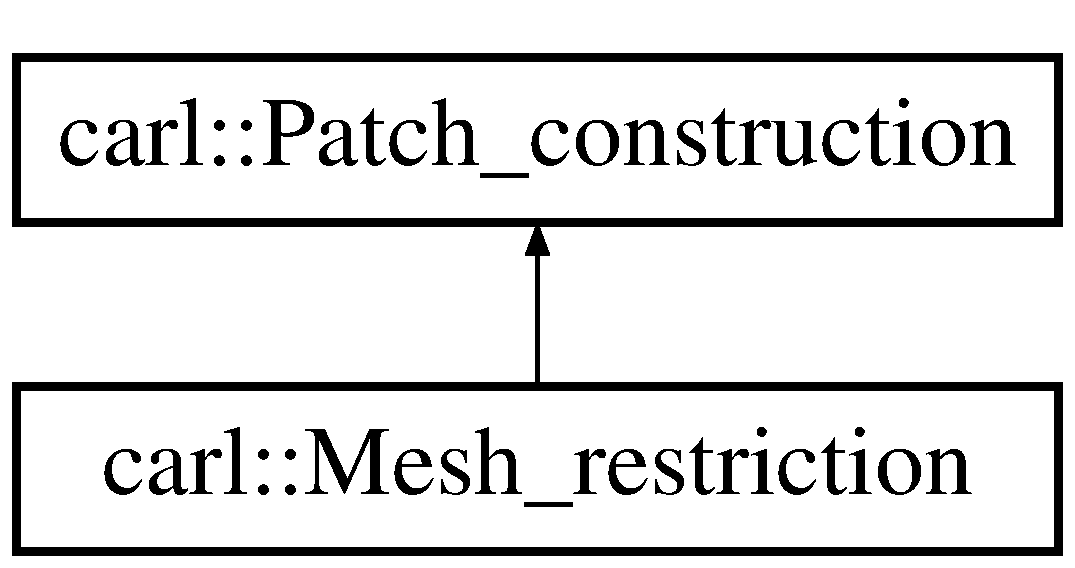
\includegraphics[height=2.000000cm]{classcarl_1_1_mesh__restriction}
\end{center}
\end{figure}
\subsection*{Public Member Functions}
\begin{DoxyCompactItemize}
\item 
\hyperlink{classcarl_1_1_mesh__restriction_a8999a74445ddd927a357725137444286}{Mesh\+\_\+restriction} (lib\+Mesh\+::\+Mesh \&mesh, const lib\+Mesh\+::\+Parallel\+::\+Communicator \&local\+\_\+comm, bool debug\+Output=false)
\begin{DoxyCompactList}\small\item\em Constructor with a pre-\/defined parent mesh and a local communicator. \end{DoxyCompactList}\item 
void \hyperlink{classcarl_1_1_mesh__restriction_adce7d5a94e5e65f5bee4145eb25ebd61}{Build\+Restriction} (const lib\+Mesh\+::\+Replicated\+Mesh \&Coupling\+\_\+mesh)
\begin{DoxyCompactList}\small\item\em Build the restriction of the parent mesh to the coupling region defined by Coupling\+\_\+mesh. \end{DoxyCompactList}\item 
lib\+Mesh\+::\+Replicated\+Mesh \& \hyperlink{classcarl_1_1_mesh__restriction_a1313c9ef12044e000a03b35b379b56bc}{restricted\+\_\+mesh} ()
\begin{DoxyCompactList}\small\item\em Returns the restricted mesh. \end{DoxyCompactList}\item 
void \hyperlink{classcarl_1_1_mesh__restriction_aacd0d990d392ea65c027974d380bbc26}{export\+\_\+restriction\+\_\+mesh} (const std\+::string \&filename\+\_\+base)
\begin{DoxyCompactList}\small\item\em Export the restricted mesh to a file. \end{DoxyCompactList}\item 
void \hyperlink{classcarl_1_1_mesh__restriction_ab2253edf0b64fd412503b021da24f66d}{Build\+Restriction\+From\+Set} (const std\+::unordered\+\_\+set$<$ unsigned int $>$ $\ast$restricted\+\_\+mesh\+\_\+set)
\begin{DoxyCompactList}\small\item\em Build the restriction of the parent mesh from a given element set. This version is useful if the intersection search was already done. \end{DoxyCompactList}\end{DoxyCompactItemize}
\subsection*{Additional Inherited Members}


\subsection{Detailed Description}
Class used to build a restriction of a parent mesh to the coupling region. 

This class is derived from the \hyperlink{classcarl_1_1_patch__construction}{carl\+::\+Patch\+\_\+construction} class, and it contains the methods needed to restrict a mesh to the region defined by the coupling mesh. 

Definition at line 31 of file restrict\+\_\+mesh.\+h.



\subsection{Constructor \& Destructor Documentation}
\hypertarget{classcarl_1_1_mesh__restriction_a8999a74445ddd927a357725137444286}{}\index{carl\+::\+Mesh\+\_\+restriction@{carl\+::\+Mesh\+\_\+restriction}!Mesh\+\_\+restriction@{Mesh\+\_\+restriction}}
\index{Mesh\+\_\+restriction@{Mesh\+\_\+restriction}!carl\+::\+Mesh\+\_\+restriction@{carl\+::\+Mesh\+\_\+restriction}}
\subsubsection[{Mesh\+\_\+restriction(lib\+Mesh\+::\+Mesh \&mesh, const lib\+Mesh\+::\+Parallel\+::\+Communicator \&local\+\_\+comm, bool debug\+Output=false)}]{\setlength{\rightskip}{0pt plus 5cm}carl\+::\+Mesh\+\_\+restriction\+::\+Mesh\+\_\+restriction (
\begin{DoxyParamCaption}
\item[{lib\+Mesh\+::\+Mesh \&}]{mesh, }
\item[{const lib\+Mesh\+::\+Parallel\+::\+Communicator \&}]{local\+\_\+comm, }
\item[{bool}]{debug\+Output = {\ttfamily false}}
\end{DoxyParamCaption}
)\hspace{0.3cm}{\ttfamily [inline]}}\label{classcarl_1_1_mesh__restriction_a8999a74445ddd927a357725137444286}


Constructor with a pre-\/defined parent mesh and a local communicator. 



Definition at line 37 of file restrict\+\_\+mesh.\+h.


\begin{DoxyCode}
38     : \hyperlink{classcarl_1_1_patch__construction_a78474f4c77674b43140c4aa77a0c255a}{Patch\_construction}(mesh, local\_comm, debugOutput)
39     \{
40 
41     \};
\end{DoxyCode}


\subsection{Member Function Documentation}
\hypertarget{classcarl_1_1_mesh__restriction_adce7d5a94e5e65f5bee4145eb25ebd61}{}\index{carl\+::\+Mesh\+\_\+restriction@{carl\+::\+Mesh\+\_\+restriction}!Build\+Restriction@{Build\+Restriction}}
\index{Build\+Restriction@{Build\+Restriction}!carl\+::\+Mesh\+\_\+restriction@{carl\+::\+Mesh\+\_\+restriction}}
\subsubsection[{Build\+Restriction(const lib\+Mesh\+::\+Replicated\+Mesh \&\+Coupling\+\_\+mesh)}]{\setlength{\rightskip}{0pt plus 5cm}void carl\+::\+Mesh\+\_\+restriction\+::\+Build\+Restriction (
\begin{DoxyParamCaption}
\item[{const lib\+Mesh\+::\+Replicated\+Mesh \&}]{Coupling\+\_\+mesh}
\end{DoxyParamCaption}
)}\label{classcarl_1_1_mesh__restriction_adce7d5a94e5e65f5bee4145eb25ebd61}


Build the restriction of the parent mesh to the coupling region defined by Coupling\+\_\+mesh. 



Definition at line 36 of file restrict\+\_\+mesh.\+cpp.


\begin{DoxyCode}
37 \{
38     \textcolor{keywordtype}{bool} bDoIntersect = \textcolor{keyword}{false};
39 
40     \textcolor{comment}{// Deque containing the indices of the elements to test}
41     std::deque<int> Restriction\_Test\_Queue;
42 
43     \textcolor{comment}{// Unordered set, used to avoid double testing elements}
44     \textcolor{keywordtype}{unsigned} \textcolor{keywordtype}{int} treated\_from\_mesh\_preallocation = \hyperlink{classcarl_1_1_patch__construction_aec2f60b62d5d7b44bfcc4f9ca9de28d2}{m\_Mesh\_parent}.n\_elem();
45     std::unordered\_set<int> Treated\_From\_Mesh;
46 
47     \textcolor{comment}{// Only do the work over a single processor, to avoid communications.}
48     \textcolor{keywordflow}{if}(\hyperlink{classcarl_1_1_patch__construction_abb348e12e9fb16cb426e68127ec02c95}{m\_rank} ==0)
49     \{
50         Treated\_From\_Mesh.reserve(treated\_from\_mesh\_preallocation);
51 
52         std::set<unsigned int> Intersecting\_elems;
53 
54         \textcolor{comment}{// Index and pointer to element being tested right now}
55         \textcolor{keywordtype}{unsigned} \textcolor{keywordtype}{int}    Tested\_idx;
56 
57         \textcolor{comment}{// Candidate index}
58         \textcolor{keywordtype}{unsigned} \textcolor{keywordtype}{int}    Candidate\_idx;
59 
60         \hyperlink{classcarl_1_1_patch__construction_af7db498027d46bff8464757e824404fb}{m\_Patch\_Elem\_indexes}.clear();
61         \hyperlink{classcarl_1_1_patch__construction_a85fb959e6f57d935a8d6fe0d4f0f7f46}{m\_Patch\_Node\_indexes}.clear();
62         \hyperlink{classcarl_1_1_patch__construction_a47c4343835537781c48813feed01e60e}{m\_Patch\_Elem\_Neighbours}.clear();
63 
64         std::set<unsigned int>::iterator it\_set\_start;
65 
66         libMesh::Mesh::const\_element\_iterator it\_coupling = Coupling\_mesh.elements\_begin();
67         libMesh::Mesh::const\_element\_iterator it\_coupling\_end = Coupling\_mesh.elements\_end();
68 
69         \textcolor{comment}{// Debug vars}
70         \textcolor{keywordtype}{int} nbOfTests = 1;
71         \textcolor{keywordtype}{int} nbOfPositiveTests = 1;
72 
73         \textcolor{keywordflow}{for}( ; it\_coupling != it\_coupling\_end; ++it\_coupling)
74         \{
75             \textcolor{keyword}{const} libMesh::Elem * Query\_elem = * it\_coupling;
76 
77             Treated\_From\_Mesh.clear();
78 
79             \textcolor{comment}{// Find elements from the original mesh intersecting the coupling element}
80             \hyperlink{classcarl_1_1_patch__construction_a59f947d3d18761b1ad1a5913eb59ca83}{m\_Intersection\_Test}.\hyperlink{classcarl_1_1_intersection___tools_a8238069bd83ef1029c6a5b60a188763b}{FindAllIntersection}(Query\_elem,
      \hyperlink{classcarl_1_1_patch__construction_a382e1ea46006b1ea6445af758e157ceb}{m\_Parent\_Point\_Locator},Intersecting\_elems);
81 
82             libMesh::Elem *     First\_Restriction\_elems = NULL;
83             libMesh::Elem *     elem\_candidate = NULL;
84             it\_set\_start      = Intersecting\_elems.begin();
85 
86             \textcolor{keywordflow}{for}( ; it\_set\_start != Intersecting\_elems.end(); ++it\_set\_start)
87             \{
88                 Treated\_From\_Mesh.insert(*it\_set\_start);
89                 First\_Restriction\_elems = \hyperlink{classcarl_1_1_patch__construction_aec2f60b62d5d7b44bfcc4f9ca9de28d2}{m\_Mesh\_parent}.elem(*it\_set\_start);
90                 \hyperlink{classcarl_1_1_patch__construction_ae7a46ef950445a82cb0036b49b778fbf}{insert\_patch\_element}(First\_Restriction\_elems);
91 
92                 \textcolor{keywordflow}{for}(\textcolor{keywordtype}{unsigned} \textcolor{keywordtype}{int} iii = 0; iii < First\_Restriction\_elems->n\_neighbors(); ++iii)
93                 \{
94                     elem\_candidate = First\_Restriction\_elems->neighbor(iii);
95                     \textcolor{keywordflow}{if}(elem\_candidate != NULL && Treated\_From\_Mesh.find(elem\_candidate->id())==
      Treated\_From\_Mesh.end())
96                     \{
97                         Restriction\_Test\_Queue.push\_back(elem\_candidate->id());
98                         Treated\_From\_Mesh.insert(elem\_candidate->id());
99                     \}
100                 \}
101             \}
102 
103             \textcolor{keywordflow}{while}(!Restriction\_Test\_Queue.empty())
104             \{
105                 \textcolor{comment}{// Extract element from the list}
106                 Tested\_idx = Restriction\_Test\_Queue[0];
107                 Restriction\_Test\_Queue.pop\_front();
108                 \textcolor{keyword}{const} libMesh::Elem     * Tested\_elem = \hyperlink{classcarl_1_1_patch__construction_aec2f60b62d5d7b44bfcc4f9ca9de28d2}{m\_Mesh\_parent}.elem(Tested\_idx);
109 
110                 \textcolor{comment}{// Test it}
111                 bDoIntersect = \hyperlink{classcarl_1_1_patch__construction_a59f947d3d18761b1ad1a5913eb59ca83}{m\_Intersection\_Test}.
      \hyperlink{classcarl_1_1_intersection___tools_ae7b16748a45a0579bafecb48ef2fc4ce}{libMesh\_exact\_do\_intersect}(Query\_elem,Tested\_elem);
112                 ++nbOfTests;
113 
114                 \textcolor{comment}{// If it does intersect ...}
115                 \textcolor{keywordflow}{if}(bDoIntersect)
116                 \{
117                     ++nbOfPositiveTests;
118 
119                     \textcolor{comment}{// Add it to the output list ...}
120                     \hyperlink{classcarl_1_1_patch__construction_ae7a46ef950445a82cb0036b49b778fbf}{insert\_patch\_element}(Tested\_elem);
121 
122                     \textcolor{comment}{// ... And add its neighbours (if they weren't tested yet)}
123                     \textcolor{keywordflow}{for}(\textcolor{keywordtype}{unsigned} \textcolor{keywordtype}{int} iii = 0; iii < Tested\_elem->n\_neighbors(); ++iii)
124                     \{
125                         elem\_candidate = Tested\_elem->neighbor(iii);
126                         \textcolor{keywordflow}{if}(elem\_candidate != NULL)
127                         \{
128                             Candidate\_idx = elem\_candidate->id();
129                             \textcolor{keywordflow}{if}(Treated\_From\_Mesh.find(Candidate\_idx)==Treated\_From\_Mesh.end())
130                             \{
131                                 Restriction\_Test\_Queue.push\_back(Candidate\_idx);
132                                 Treated\_From\_Mesh.insert(Candidate\_idx);
133                             \}
134                         \}
135                     \}
136                 \}
137             \}
138         \}
139 
140         this->\hyperlink{classcarl_1_1_patch__construction_ab4e5b3f8e8f2a7c0af44979a8b0a39c4}{build\_patch\_mesh}();
141 
142         \textcolor{keywordflow}{if}(\hyperlink{classcarl_1_1_patch__construction_a93158e5a81432eb8f92860552bff37bc}{m\_bPrintDebug})
143         \{
144             std::cout << \textcolor{stringliteral}{"    DEBUG: Restriction search results"} << std::endl;
145             std::cout << \textcolor{stringliteral}{" -> Nb. of intersections found  : "} << 
      \hyperlink{classcarl_1_1_patch__construction_af7db498027d46bff8464757e824404fb}{m\_Patch\_Elem\_indexes}.size() << std::endl << std::endl;
146 
147             std::cout << \textcolor{stringliteral}{" -> Nb. of mesh elements        : "} << \hyperlink{classcarl_1_1_patch__construction_aec2f60b62d5d7b44bfcc4f9ca9de28d2}{m\_Mesh\_parent}.n\_elem() << 
      std::endl;
148             std::cout << \textcolor{stringliteral}{" -> Nb. of Restriction elements : "} << 
      \hyperlink{classcarl_1_1_patch__construction_af7db498027d46bff8464757e824404fb}{m\_Patch\_Elem\_indexes}.size() << std::endl;
149             std::cout << \textcolor{stringliteral}{" -> Patch elem %                : "} << 100.*
      \hyperlink{classcarl_1_1_patch__construction_af7db498027d46bff8464757e824404fb}{m\_Patch\_Elem\_indexes}.size()/\hyperlink{classcarl_1_1_patch__construction_aec2f60b62d5d7b44bfcc4f9ca9de28d2}{m\_Mesh\_parent}.n\_elem() << \textcolor{stringliteral}{" %"} << std::endl <<
       std::endl;
150 
151             std::cout << \textcolor{stringliteral}{" -> Nb. of mesh nodes           : "} << \hyperlink{classcarl_1_1_patch__construction_aec2f60b62d5d7b44bfcc4f9ca9de28d2}{m\_Mesh\_parent}.n\_nodes() << 
      std::endl;
152             std::cout << \textcolor{stringliteral}{" -> Nb. of patch nodes          : "} << 
      \hyperlink{classcarl_1_1_patch__construction_a85fb959e6f57d935a8d6fe0d4f0f7f46}{m\_Patch\_Node\_indexes}.size() << std::endl;
153             std::cout << \textcolor{stringliteral}{" -> Patch node %                : "} << 100.*
      \hyperlink{classcarl_1_1_patch__construction_a85fb959e6f57d935a8d6fe0d4f0f7f46}{m\_Patch\_Node\_indexes}.size()/\hyperlink{classcarl_1_1_patch__construction_aec2f60b62d5d7b44bfcc4f9ca9de28d2}{m\_Mesh\_parent}.n\_nodes() << \textcolor{stringliteral}{" %"} << std::endl <
      < std::endl;
154 
155             std::cout << \textcolor{stringliteral}{" -> Nb. of tests                : "} << nbOfTests << std::endl;
156             std::cout << \textcolor{stringliteral}{" -> Nb. of positive tests       : "} << nbOfPositiveTests << std::endl;
157             std::cout << \textcolor{stringliteral}{" -> Positive %                  : "} << 100.*nbOfPositiveTests/nbOfTests << \textcolor{stringliteral}{" %"} <
      < std::endl << std::endl;
158         \}
159     \}
160 \}
\end{DoxyCode}
\hypertarget{classcarl_1_1_mesh__restriction_ab2253edf0b64fd412503b021da24f66d}{}\index{carl\+::\+Mesh\+\_\+restriction@{carl\+::\+Mesh\+\_\+restriction}!Build\+Restriction\+From\+Set@{Build\+Restriction\+From\+Set}}
\index{Build\+Restriction\+From\+Set@{Build\+Restriction\+From\+Set}!carl\+::\+Mesh\+\_\+restriction@{carl\+::\+Mesh\+\_\+restriction}}
\subsubsection[{Build\+Restriction\+From\+Set(const std\+::unordered\+\_\+set$<$ unsigned int $>$ $\ast$restricted\+\_\+mesh\+\_\+set)}]{\setlength{\rightskip}{0pt plus 5cm}void carl\+::\+Mesh\+\_\+restriction\+::\+Build\+Restriction\+From\+Set (
\begin{DoxyParamCaption}
\item[{const std\+::unordered\+\_\+set$<$ unsigned int $>$ $\ast$}]{restricted\+\_\+mesh\+\_\+set}
\end{DoxyParamCaption}
)}\label{classcarl_1_1_mesh__restriction_ab2253edf0b64fd412503b021da24f66d}


Build the restriction of the parent mesh from a given element set. This version is useful if the intersection search was already done. 



Definition at line 12 of file restrict\+\_\+mesh.\+cpp.


\begin{DoxyCode}
13 \{
14     \textcolor{comment}{// Intersection and distribution work done already by the stitch algorithm.}
15 
16     \textcolor{comment}{// Only do the work over a single processor, to avoid communications.}
17     \textcolor{keywordflow}{if}(\hyperlink{classcarl_1_1_patch__construction_abb348e12e9fb16cb426e68127ec02c95}{m\_rank} == 0)
18     \{
19         \hyperlink{classcarl_1_1_patch__construction_af7db498027d46bff8464757e824404fb}{m\_Patch\_Elem\_indexes}.clear();
20         \hyperlink{classcarl_1_1_patch__construction_a85fb959e6f57d935a8d6fe0d4f0f7f46}{m\_Patch\_Node\_indexes}.clear();
21         \hyperlink{classcarl_1_1_patch__construction_a47c4343835537781c48813feed01e60e}{m\_Patch\_Elem\_Neighbours}.clear();
22 
23         std::unordered\_set<unsigned int >::const\_iterator elem\_idx\_it = restricted\_mesh\_set->begin();
24         std::unordered\_set<unsigned int >::const\_iterator elem\_idx\_it\_end = restricted\_mesh\_set->end();
25 
26         \textcolor{keywordflow}{for}( ; elem\_idx\_it != elem\_idx\_it\_end; ++ elem\_idx\_it)
27         \{
28             \textcolor{keyword}{const} libMesh::Elem * elem\_to\_add = \hyperlink{classcarl_1_1_patch__construction_aec2f60b62d5d7b44bfcc4f9ca9de28d2}{m\_Mesh\_parent}.elem(*elem\_idx\_it);
29             \hyperlink{classcarl_1_1_patch__construction_ae7a46ef950445a82cb0036b49b778fbf}{insert\_patch\_element}(elem\_to\_add);
30         \}
31 
32         this->\hyperlink{classcarl_1_1_patch__construction_ab4e5b3f8e8f2a7c0af44979a8b0a39c4}{build\_patch\_mesh}();
33     \}
34 \}
\end{DoxyCode}
\hypertarget{classcarl_1_1_mesh__restriction_aacd0d990d392ea65c027974d380bbc26}{}\index{carl\+::\+Mesh\+\_\+restriction@{carl\+::\+Mesh\+\_\+restriction}!export\+\_\+restriction\+\_\+mesh@{export\+\_\+restriction\+\_\+mesh}}
\index{export\+\_\+restriction\+\_\+mesh@{export\+\_\+restriction\+\_\+mesh}!carl\+::\+Mesh\+\_\+restriction@{carl\+::\+Mesh\+\_\+restriction}}
\subsubsection[{export\+\_\+restriction\+\_\+mesh(const std\+::string \&filename\+\_\+base)}]{\setlength{\rightskip}{0pt plus 5cm}void carl\+::\+Mesh\+\_\+restriction\+::export\+\_\+restriction\+\_\+mesh (
\begin{DoxyParamCaption}
\item[{const std\+::string \&}]{filename\+\_\+base}
\end{DoxyParamCaption}
)}\label{classcarl_1_1_mesh__restriction_aacd0d990d392ea65c027974d380bbc26}


Export the restricted mesh to a file. 



Definition at line 162 of file restrict\+\_\+mesh.\+cpp.


\begin{DoxyCode}
163 \{
164     \textcolor{keywordflow}{if}(\hyperlink{classcarl_1_1_patch__construction_abb348e12e9fb16cb426e68127ec02c95}{m\_rank} == 0)
165     \{
166         std::string filename\_mesh = filename\_base + \textcolor{stringliteral}{".msh"};
167 
168         \textcolor{comment}{// Print mesh}
169         libMesh::GmshIO output\_mesh(\hyperlink{classcarl_1_1_patch__construction_a4dfae5a2c4a983ac31dacec1cdb29d11}{m\_Mesh\_patch});
170         output\_mesh.binary() = \textcolor{keyword}{true};
171         output\_mesh.write(filename\_mesh);
172 
173         std::string filename\_elements = filename\_base + \textcolor{stringliteral}{"\_restrict.dat"};
174 
175         std::ofstream elems\_out(filename\_elements);
176 
177         elems\_out << \hyperlink{classcarl_1_1_patch__construction_a801e75fa9573645a57d24b996611fe4d}{m\_elem\_map\_Patch\_to\_Parent}.size() << std::endl;
178         \textcolor{keywordflow}{for}(\textcolor{keywordtype}{unsigned} \textcolor{keywordtype}{int} iii = 0; iii < \hyperlink{classcarl_1_1_patch__construction_a801e75fa9573645a57d24b996611fe4d}{m\_elem\_map\_Patch\_to\_Parent}.size(); ++iii)
179         \{
180             elems\_out << iii << \textcolor{stringliteral}{" "} << \hyperlink{classcarl_1_1_patch__construction_a801e75fa9573645a57d24b996611fe4d}{m\_elem\_map\_Patch\_to\_Parent}[iii] << 
      std::endl;
181         \}
182 
183         elems\_out.close();
184     \}
185 \}
\end{DoxyCode}
\hypertarget{classcarl_1_1_mesh__restriction_a1313c9ef12044e000a03b35b379b56bc}{}\index{carl\+::\+Mesh\+\_\+restriction@{carl\+::\+Mesh\+\_\+restriction}!restricted\+\_\+mesh@{restricted\+\_\+mesh}}
\index{restricted\+\_\+mesh@{restricted\+\_\+mesh}!carl\+::\+Mesh\+\_\+restriction@{carl\+::\+Mesh\+\_\+restriction}}
\subsubsection[{restricted\+\_\+mesh()}]{\setlength{\rightskip}{0pt plus 5cm}lib\+Mesh\+::\+Replicated\+Mesh \& carl\+::\+Mesh\+\_\+restriction\+::restricted\+\_\+mesh (
\begin{DoxyParamCaption}
{}
\end{DoxyParamCaption}
)}\label{classcarl_1_1_mesh__restriction_a1313c9ef12044e000a03b35b379b56bc}


Returns the restricted mesh. 



Definition at line 187 of file restrict\+\_\+mesh.\+cpp.


\begin{DoxyCode}
188 \{
189     \textcolor{keywordflow}{return} \hyperlink{classcarl_1_1_patch__construction_a4dfae5a2c4a983ac31dacec1cdb29d11}{m\_Mesh\_patch};
190 \}
\end{DoxyCode}


The documentation for this class was generated from the following files\+:\begin{DoxyCompactItemize}
\item 
/\+Users/breubreubreu/\+Programming/\+C\+Arl/\+Cpp/src/include/\hyperlink{restrict__mesh_8h}{restrict\+\_\+mesh.\+h}\item 
/\+Users/breubreubreu/\+Programming/\+C\+Arl/\+Cpp/src/common/intersections\+\_\+parallel/\hyperlink{restrict__mesh_8cpp}{restrict\+\_\+mesh.\+cpp}\end{DoxyCompactItemize}

\hypertarget{class_order4_tensor}{}\section{Order4\+Tensor Class Reference}
\label{class_order4_tensor}\index{Order4\+Tensor@{Order4\+Tensor}}


{\ttfamily \#include $<$anisotropic\+\_\+elasticity\+\_\+cubic\+\_\+sym.\+h$>$}

\subsection*{Public Member Functions}
\begin{DoxyCompactItemize}
\item 
\hyperlink{class_order4_tensor_a3f8130422a7e64a9d1dbe764d5bee4e2}{Order4\+Tensor} ()
\item 
\hyperlink{class_order4_tensor_a91ac3e32ce3ad0e4334699e77783a295}{Order4\+Tensor} (int dim)
\item 
void \hyperlink{class_order4_tensor_af1900935b9a3e18edf46c24bac6027af}{set\+\_\+dimension} (int dim)
\item 
lib\+Mesh\+::\+Real \& \hyperlink{class_order4_tensor_ae2e5d607539ad64353deda3bb6ec623b}{operator()} (unsigned int iii, unsigned int jjj, unsigned int kkk, unsigned int lll)
\end{DoxyCompactItemize}
\subsection*{Public Attributes}
\begin{DoxyCompactItemize}
\item 
std\+::vector$<$ lib\+Mesh\+::\+Real $>$ \hyperlink{class_order4_tensor_acec0c420962426e3104218af2ad02b4d}{vector}
\end{DoxyCompactItemize}


\subsection{Detailed Description}


Definition at line 13 of file anisotropic\+\_\+elasticity\+\_\+cubic\+\_\+sym.\+h.



\subsection{Constructor \& Destructor Documentation}
\hypertarget{class_order4_tensor_a3f8130422a7e64a9d1dbe764d5bee4e2}{}\index{Order4\+Tensor@{Order4\+Tensor}!Order4\+Tensor@{Order4\+Tensor}}
\index{Order4\+Tensor@{Order4\+Tensor}!Order4\+Tensor@{Order4\+Tensor}}
\subsubsection[{Order4\+Tensor()}]{\setlength{\rightskip}{0pt plus 5cm}Order4\+Tensor\+::\+Order4\+Tensor (
\begin{DoxyParamCaption}
{}
\end{DoxyParamCaption}
)\hspace{0.3cm}{\ttfamily [inline]}}\label{class_order4_tensor_a3f8130422a7e64a9d1dbe764d5bee4e2}


Definition at line 21 of file anisotropic\+\_\+elasticity\+\_\+cubic\+\_\+sym.\+h.


\begin{DoxyCode}
21                    :
22         m\_dim \{ 0 \},
23         m\_idx \{ 0 \}
24     \{
25 
26     \};
\end{DoxyCode}
\hypertarget{class_order4_tensor_a91ac3e32ce3ad0e4334699e77783a295}{}\index{Order4\+Tensor@{Order4\+Tensor}!Order4\+Tensor@{Order4\+Tensor}}
\index{Order4\+Tensor@{Order4\+Tensor}!Order4\+Tensor@{Order4\+Tensor}}
\subsubsection[{Order4\+Tensor(int dim)}]{\setlength{\rightskip}{0pt plus 5cm}Order4\+Tensor\+::\+Order4\+Tensor (
\begin{DoxyParamCaption}
\item[{int}]{dim}
\end{DoxyParamCaption}
)\hspace{0.3cm}{\ttfamily [inline]}}\label{class_order4_tensor_a91ac3e32ce3ad0e4334699e77783a295}


Definition at line 28 of file anisotropic\+\_\+elasticity\+\_\+cubic\+\_\+sym.\+h.


\begin{DoxyCode}
28                           :
29         m\_idx \{ 0 \}
30     \{
31         m\_dim = dim;
32         \hyperlink{class_order4_tensor_af1900935b9a3e18edf46c24bac6027af}{set\_dimension}(dim);
33     \};
\end{DoxyCode}


\subsection{Member Function Documentation}
\hypertarget{class_order4_tensor_ae2e5d607539ad64353deda3bb6ec623b}{}\index{Order4\+Tensor@{Order4\+Tensor}!operator()@{operator()}}
\index{operator()@{operator()}!Order4\+Tensor@{Order4\+Tensor}}
\subsubsection[{operator()(unsigned int iii, unsigned int jjj, unsigned int kkk, unsigned int lll)}]{\setlength{\rightskip}{0pt plus 5cm}lib\+Mesh\+::\+Real \& Order4\+Tensor\+::operator() (
\begin{DoxyParamCaption}
\item[{unsigned int}]{iii, }
\item[{unsigned int}]{jjj, }
\item[{unsigned int}]{kkk, }
\item[{unsigned int}]{lll}
\end{DoxyParamCaption}
)\hspace{0.3cm}{\ttfamily [inline]}}\label{class_order4_tensor_ae2e5d607539ad64353deda3bb6ec623b}


Definition at line 51 of file anisotropic\+\_\+elasticity\+\_\+cubic\+\_\+sym.\+h.


\begin{DoxyCode}
52 \{
53     m\_idx =   m\_idx\_mult[0] * iii
54             + m\_idx\_mult[1] * jjj
55             + m\_idx\_mult[2] * kkk
56             + m\_idx\_mult[3] * lll;
57     \textcolor{keywordflow}{return} \hyperlink{class_order4_tensor_acec0c420962426e3104218af2ad02b4d}{vector}[m\_idx];
58 \}
\end{DoxyCode}
\hypertarget{class_order4_tensor_af1900935b9a3e18edf46c24bac6027af}{}\index{Order4\+Tensor@{Order4\+Tensor}!set\+\_\+dimension@{set\+\_\+dimension}}
\index{set\+\_\+dimension@{set\+\_\+dimension}!Order4\+Tensor@{Order4\+Tensor}}
\subsubsection[{set\+\_\+dimension(int dim)}]{\setlength{\rightskip}{0pt plus 5cm}void Order4\+Tensor\+::set\+\_\+dimension (
\begin{DoxyParamCaption}
\item[{int}]{dim}
\end{DoxyParamCaption}
)\hspace{0.3cm}{\ttfamily [inline]}}\label{class_order4_tensor_af1900935b9a3e18edf46c24bac6027af}


Definition at line 37 of file anisotropic\+\_\+elasticity\+\_\+cubic\+\_\+sym.\+h.


\begin{DoxyCode}
38     \{
39         m\_dim = dim;
40         m\_idx\_mult.resize(4);
41         \hyperlink{class_order4_tensor_acec0c420962426e3104218af2ad02b4d}{vector}.resize(std::pow(m\_dim,4),0);
42 
43         \textcolor{keywordflow}{for}(\textcolor{keywordtype}{int} iii = 0; iii < 4; ++iii)
44         \{
45             m\_idx\_mult[iii] = std::pow(m\_dim,iii);
46         \}
47     \}
\end{DoxyCode}


\subsection{Member Data Documentation}
\hypertarget{class_order4_tensor_acec0c420962426e3104218af2ad02b4d}{}\index{Order4\+Tensor@{Order4\+Tensor}!vector@{vector}}
\index{vector@{vector}!Order4\+Tensor@{Order4\+Tensor}}
\subsubsection[{vector}]{\setlength{\rightskip}{0pt plus 5cm}std\+::vector$<$lib\+Mesh\+::\+Real$>$ Order4\+Tensor\+::vector}\label{class_order4_tensor_acec0c420962426e3104218af2ad02b4d}


Definition at line 33 of file anisotropic\+\_\+elasticity\+\_\+cubic\+\_\+sym.\+h.



The documentation for this class was generated from the following file\+:\begin{DoxyCompactItemize}
\item 
/\+Users/breubreubreu/\+Programming/\+C\+Arl/\+Cpp/src/execs/ext\+\_\+solver\+\_\+libmesh/ext\+\_\+solver\+\_\+libmesh\+\_\+common/\+N\+O\+T\+\_\+\+R\+E\+A\+D\+Y\+\_\+\+Y\+E\+T/\hyperlink{anisotropic__elasticity__cubic__sym_8h}{anisotropic\+\_\+elasticity\+\_\+cubic\+\_\+sym.\+h}\end{DoxyCompactItemize}

\hypertarget{structcarl_1_1parallel__intersection__params}{}\section{carl\+:\+:parallel\+\_\+intersection\+\_\+params Struct Reference}
\label{structcarl_1_1parallel__intersection__params}\index{carl\+::parallel\+\_\+intersection\+\_\+params@{carl\+::parallel\+\_\+intersection\+\_\+params}}


Structure containing the parameters for the parallel intersection search test program (source\+: \hyperlink{_c_arl__build__intersections_8cpp}{C\+Arl\+\_\+build\+\_\+intersections.\+cpp})  




{\ttfamily \#include $<$intersection\+\_\+input\+\_\+parser.\+h$>$}

\subsection*{Public Attributes}
\begin{DoxyCompactItemize}
\item 
std\+::string \hyperlink{structcarl_1_1parallel__intersection__params_aa984f7e6899406a1d17bdaa22e669e22}{mesh\+\_\+\+A}
\begin{DoxyCompactList}\small\item\em Mesh A path. \end{DoxyCompactList}\item 
std\+::string \hyperlink{structcarl_1_1parallel__intersection__params_a77a1bbaf19e80f8dfd2612c2e86acb45}{mesh\+\_\+\+B}
\begin{DoxyCompactList}\small\item\em Mesh B path. \end{DoxyCompactList}\item 
std\+::string \hyperlink{structcarl_1_1parallel__intersection__params_ad1cf6ec92655114a12be003b05526697}{mesh\+\_\+\+C}
\begin{DoxyCompactList}\small\item\em Coupling mesh path. \end{DoxyCompactList}\item 
std\+::string \hyperlink{structcarl_1_1parallel__intersection__params_a74ba855a7e3dc3595531e6204eb57db2}{output\+\_\+base}
\begin{DoxyCompactList}\small\item\em Output filename base. \end{DoxyCompactList}\item 
bool \hyperlink{structcarl_1_1parallel__intersection__params_a16529af2562e264bf3c5822d8d653b08}{b\+Stitch\+Inter\+Meshes}
\begin{DoxyCompactList}\small\item\em Stitch the intersection meshes? \end{DoxyCompactList}\item 
bool \hyperlink{structcarl_1_1parallel__intersection__params_a15197709febaff5f7082264db05d2aa7}{b\+Verbose}
\begin{DoxyCompactList}\small\item\em Print coupling partitioning? \end{DoxyCompactList}\item 
\hyperlink{namespacecarl_a4f72fd25137b97ac1ca1276ec549e5cf}{carl\+::\+Intersection\+Meshing\+Method} \hyperlink{structcarl_1_1parallel__intersection__params_ab94c6f1beb1d530141758397f49d6d08}{inter\+\_\+meshing\+\_\+method}
\begin{DoxyCompactList}\small\item\em Intersection meshing method. {\itshape Values}\+: carl\+::\+Intersection\+Meshing\+Method\+::\+C\+G\+A\+L or carl\+::\+Intersection\+Meshing\+Method\+::\+L\+I\+B\+M\+E\+S\+H\+\_\+\+T\+E\+T\+G\+E\+N. \end{DoxyCompactList}\end{DoxyCompactItemize}


\subsection{Detailed Description}
Structure containing the parameters for the parallel intersection search test program (source\+: \hyperlink{_c_arl__build__intersections_8cpp}{C\+Arl\+\_\+build\+\_\+intersections.\+cpp}) 

Details on the parameters setup are found in the documentation of \hyperlink{namespacecarl_ab80eec3eb20ff6a403ad01bafa649df2}{carl\+::get\+\_\+intersection\+\_\+input\+\_\+params}(Get\+Pot\& field\+\_\+parser, \hyperlink{structcarl_1_1parallel__intersection__params}{parallel\+\_\+intersection\+\_\+params}\& input\+\_\+params). 

Definition at line 23 of file intersection\+\_\+input\+\_\+parser.\+h.



\subsection{Member Data Documentation}
\hypertarget{structcarl_1_1parallel__intersection__params_a16529af2562e264bf3c5822d8d653b08}{}\index{carl\+::parallel\+\_\+intersection\+\_\+params@{carl\+::parallel\+\_\+intersection\+\_\+params}!b\+Stitch\+Inter\+Meshes@{b\+Stitch\+Inter\+Meshes}}
\index{b\+Stitch\+Inter\+Meshes@{b\+Stitch\+Inter\+Meshes}!carl\+::parallel\+\_\+intersection\+\_\+params@{carl\+::parallel\+\_\+intersection\+\_\+params}}
\subsubsection[{b\+Stitch\+Inter\+Meshes}]{\setlength{\rightskip}{0pt plus 5cm}bool carl\+::parallel\+\_\+intersection\+\_\+params\+::b\+Stitch\+Inter\+Meshes}\label{structcarl_1_1parallel__intersection__params_a16529af2562e264bf3c5822d8d653b08}


Stitch the intersection meshes? 



Definition at line 29 of file intersection\+\_\+input\+\_\+parser.\+h.

\hypertarget{structcarl_1_1parallel__intersection__params_a15197709febaff5f7082264db05d2aa7}{}\index{carl\+::parallel\+\_\+intersection\+\_\+params@{carl\+::parallel\+\_\+intersection\+\_\+params}!b\+Verbose@{b\+Verbose}}
\index{b\+Verbose@{b\+Verbose}!carl\+::parallel\+\_\+intersection\+\_\+params@{carl\+::parallel\+\_\+intersection\+\_\+params}}
\subsubsection[{b\+Verbose}]{\setlength{\rightskip}{0pt plus 5cm}bool carl\+::parallel\+\_\+intersection\+\_\+params\+::b\+Verbose}\label{structcarl_1_1parallel__intersection__params_a15197709febaff5f7082264db05d2aa7}


Print coupling partitioning? 



Definition at line 30 of file intersection\+\_\+input\+\_\+parser.\+h.

\hypertarget{structcarl_1_1parallel__intersection__params_ab94c6f1beb1d530141758397f49d6d08}{}\index{carl\+::parallel\+\_\+intersection\+\_\+params@{carl\+::parallel\+\_\+intersection\+\_\+params}!inter\+\_\+meshing\+\_\+method@{inter\+\_\+meshing\+\_\+method}}
\index{inter\+\_\+meshing\+\_\+method@{inter\+\_\+meshing\+\_\+method}!carl\+::parallel\+\_\+intersection\+\_\+params@{carl\+::parallel\+\_\+intersection\+\_\+params}}
\subsubsection[{inter\+\_\+meshing\+\_\+method}]{\setlength{\rightskip}{0pt plus 5cm}{\bf carl\+::\+Intersection\+Meshing\+Method} carl\+::parallel\+\_\+intersection\+\_\+params\+::inter\+\_\+meshing\+\_\+method}\label{structcarl_1_1parallel__intersection__params_ab94c6f1beb1d530141758397f49d6d08}


Intersection meshing method. {\itshape Values}\+: carl\+::\+Intersection\+Meshing\+Method\+::\+C\+G\+A\+L or carl\+::\+Intersection\+Meshing\+Method\+::\+L\+I\+B\+M\+E\+S\+H\+\_\+\+T\+E\+T\+G\+E\+N. 



Definition at line 32 of file intersection\+\_\+input\+\_\+parser.\+h.

\hypertarget{structcarl_1_1parallel__intersection__params_aa984f7e6899406a1d17bdaa22e669e22}{}\index{carl\+::parallel\+\_\+intersection\+\_\+params@{carl\+::parallel\+\_\+intersection\+\_\+params}!mesh\+\_\+\+A@{mesh\+\_\+\+A}}
\index{mesh\+\_\+\+A@{mesh\+\_\+\+A}!carl\+::parallel\+\_\+intersection\+\_\+params@{carl\+::parallel\+\_\+intersection\+\_\+params}}
\subsubsection[{mesh\+\_\+\+A}]{\setlength{\rightskip}{0pt plus 5cm}std\+::string carl\+::parallel\+\_\+intersection\+\_\+params\+::mesh\+\_\+\+A}\label{structcarl_1_1parallel__intersection__params_aa984f7e6899406a1d17bdaa22e669e22}


Mesh A path. 



Definition at line 24 of file intersection\+\_\+input\+\_\+parser.\+h.

\hypertarget{structcarl_1_1parallel__intersection__params_a77a1bbaf19e80f8dfd2612c2e86acb45}{}\index{carl\+::parallel\+\_\+intersection\+\_\+params@{carl\+::parallel\+\_\+intersection\+\_\+params}!mesh\+\_\+\+B@{mesh\+\_\+\+B}}
\index{mesh\+\_\+\+B@{mesh\+\_\+\+B}!carl\+::parallel\+\_\+intersection\+\_\+params@{carl\+::parallel\+\_\+intersection\+\_\+params}}
\subsubsection[{mesh\+\_\+\+B}]{\setlength{\rightskip}{0pt plus 5cm}std\+::string carl\+::parallel\+\_\+intersection\+\_\+params\+::mesh\+\_\+\+B}\label{structcarl_1_1parallel__intersection__params_a77a1bbaf19e80f8dfd2612c2e86acb45}


Mesh B path. 



Definition at line 25 of file intersection\+\_\+input\+\_\+parser.\+h.

\hypertarget{structcarl_1_1parallel__intersection__params_ad1cf6ec92655114a12be003b05526697}{}\index{carl\+::parallel\+\_\+intersection\+\_\+params@{carl\+::parallel\+\_\+intersection\+\_\+params}!mesh\+\_\+\+C@{mesh\+\_\+\+C}}
\index{mesh\+\_\+\+C@{mesh\+\_\+\+C}!carl\+::parallel\+\_\+intersection\+\_\+params@{carl\+::parallel\+\_\+intersection\+\_\+params}}
\subsubsection[{mesh\+\_\+\+C}]{\setlength{\rightskip}{0pt plus 5cm}std\+::string carl\+::parallel\+\_\+intersection\+\_\+params\+::mesh\+\_\+\+C}\label{structcarl_1_1parallel__intersection__params_ad1cf6ec92655114a12be003b05526697}


Coupling mesh path. 



Definition at line 26 of file intersection\+\_\+input\+\_\+parser.\+h.

\hypertarget{structcarl_1_1parallel__intersection__params_a74ba855a7e3dc3595531e6204eb57db2}{}\index{carl\+::parallel\+\_\+intersection\+\_\+params@{carl\+::parallel\+\_\+intersection\+\_\+params}!output\+\_\+base@{output\+\_\+base}}
\index{output\+\_\+base@{output\+\_\+base}!carl\+::parallel\+\_\+intersection\+\_\+params@{carl\+::parallel\+\_\+intersection\+\_\+params}}
\subsubsection[{output\+\_\+base}]{\setlength{\rightskip}{0pt plus 5cm}std\+::string carl\+::parallel\+\_\+intersection\+\_\+params\+::output\+\_\+base}\label{structcarl_1_1parallel__intersection__params_a74ba855a7e3dc3595531e6204eb57db2}


Output filename base. 



Definition at line 27 of file intersection\+\_\+input\+\_\+parser.\+h.



The documentation for this struct was generated from the following file\+:\begin{DoxyCompactItemize}
\item 
/\+Users/breubreubreu/\+Programming/\+C\+Arl/\+Cpp/src/include/parsers/\hyperlink{intersection__input__parser_8h}{intersection\+\_\+input\+\_\+parser.\+h}\end{DoxyCompactItemize}

\hypertarget{classcarl_1_1_patch__construction}{}\section{carl\+:\+:Patch\+\_\+construction Class Reference}
\label{classcarl_1_1_patch__construction}\index{carl\+::\+Patch\+\_\+construction@{carl\+::\+Patch\+\_\+construction}}


Class used to build a mesh patch from a parent mesh and an coupling mesh element.  




{\ttfamily \#include $<$patch\+\_\+construction.\+h$>$}

Inheritance diagram for carl\+:\+:Patch\+\_\+construction\+:\begin{figure}[H]
\begin{center}
\leavevmode
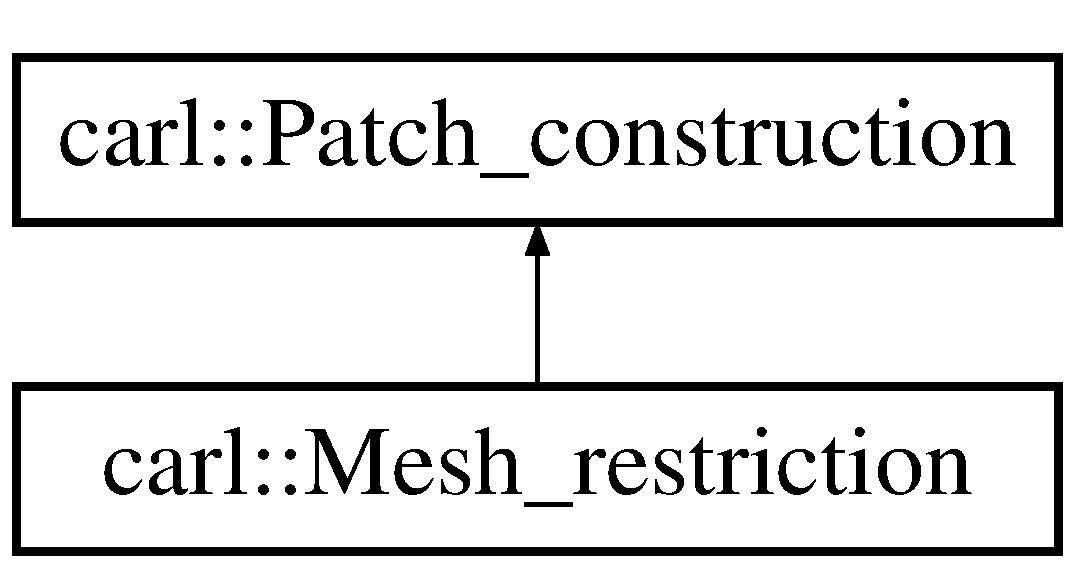
\includegraphics[height=2.000000cm]{classcarl_1_1_patch__construction}
\end{center}
\end{figure}
\subsection*{Public Member Functions}
\begin{DoxyCompactItemize}
\item 
\hyperlink{classcarl_1_1_patch__construction_ad112ac39bae272dc1572845ea5357ced}{Patch\+\_\+construction} (lib\+Mesh\+::\+Mesh \&mesh, const lib\+Mesh\+::\+Parallel\+::\+Communicator \&local\+\_\+comm, bool debug\+Output=false)
\begin{DoxyCompactList}\small\item\em Constructor with a pre-\/defined parent mesh and a local communicator. \end{DoxyCompactList}\item 
lib\+Mesh\+::\+Replicated\+Mesh \& \hyperlink{classcarl_1_1_patch__construction_a5e7fcbfddff00bd9cb431daf8288fd5a}{parent\+\_\+mesh} ()
\begin{DoxyCompactList}\small\item\em Returns the parent mesh. \end{DoxyCompactList}\item 
lib\+Mesh\+::\+Replicated\+Mesh \& \hyperlink{classcarl_1_1_patch__construction_a2b8840ec8f710a61d94638c6598e5a76}{patch\+\_\+mesh} ()
\begin{DoxyCompactList}\small\item\em Returns the patch mesh. \end{DoxyCompactList}\item 
std\+::unordered\+\_\+set$<$ unsigned int $>$ \& \hyperlink{classcarl_1_1_patch__construction_ad92eca042b223e8be1cb3984a3dc8cba}{elem\+\_\+indexes} ()
\begin{DoxyCompactList}\small\item\em Returns the set of elements inside the patch. \end{DoxyCompactList}\item 
std\+::unordered\+\_\+set$<$ unsigned int $>$ \& \hyperlink{classcarl_1_1_patch__construction_a36b55aaf8de17b8c00612907d159979e}{node\+\_\+indexes} ()
\begin{DoxyCompactList}\small\item\em Returns the set of nodes inside the patch. \end{DoxyCompactList}\item 
unsigned int \hyperlink{classcarl_1_1_patch__construction_ab9183c2cdf61de07aa77b91775286733}{size} ()
\begin{DoxyCompactList}\small\item\em Returns the number of elements inside the patch. \end{DoxyCompactList}\item 
const lib\+Mesh\+::\+Elem $\ast$ \hyperlink{classcarl_1_1_patch__construction_acb065fa34010bcf379156ccf8228e01c}{elem} (unsigned int idx)
\item 
std\+::unordered\+\_\+map$<$ unsigned int, std\+::unordered\+\_\+set$<$ unsigned int $>$ $>$ \& \hyperlink{classcarl_1_1_patch__construction_a675b7d3796e5001b86f68dbd39c2ed82}{patch\+\_\+elem\+\_\+neighbours} ()
\begin{DoxyCompactList}\small\item\em Returns the patch mesh element neighbour table. \end{DoxyCompactList}\item 
void \hyperlink{classcarl_1_1_patch__construction_aebb82c6e34f4cf38cf3e4ef2ac32b664}{Build\+Patch} (const lib\+Mesh\+::\+Elem $\ast$Query\+\_\+elem)
\begin{DoxyCompactList}\small\item\em Build the patch mesh covering a given \char`\"{}\+Query\+\_\+elem\char`\"{}. \end{DoxyCompactList}\item 
unsigned int \hyperlink{classcarl_1_1_patch__construction_a8a9aeee662261f537ed663addcce6a5a}{convert\+\_\+parent\+\_\+to\+\_\+patch\+\_\+elem\+\_\+id} (unsigned int input)
\begin{DoxyCompactList}\small\item\em Convert an element index from the parent mesh to the patch mesh. \end{DoxyCompactList}\item 
unsigned int \hyperlink{classcarl_1_1_patch__construction_a7d217e3d0eb0c2711039d019824ff5b8}{convert\+\_\+patch\+\_\+to\+\_\+parent\+\_\+elem\+\_\+id} (unsigned int input)
\begin{DoxyCompactList}\small\item\em Convert an element index from the patch mesh to the parent mesh. \end{DoxyCompactList}\item 
void \hyperlink{classcarl_1_1_patch__construction_a17cadf2879f8a7b2ef7a59dadd9d5b72}{export\+\_\+patch\+\_\+mesh} (std\+::string \&filename\+\_\+base)
\begin{DoxyCompactList}\small\item\em Export the patch mesh to a file. \end{DoxyCompactList}\item 
unsigned int \hyperlink{classcarl_1_1_patch__construction_aa2653050fa786fa5c6535bbfc5f3dbf4}{current\+\_\+elem\+\_\+id} ()
\item 
const lib\+Mesh\+::\+Elem $\ast$ \hyperlink{classcarl_1_1_patch__construction_afdf767feed130d2a9b58dc586e5d3a20}{current\+\_\+elem\+\_\+pointer} ()
\item 
void \hyperlink{classcarl_1_1_patch__construction_abc44a4dda847749fcbc2ba02d2e0a203}{intersection\+\_\+queue\+\_\+push\+\_\+back} (unsigned int elem\+\_\+id)
\begin{DoxyCompactList}\small\item\em \mbox{[}A\+D\+V. F\+R\+O\+N\+T\mbox{]} Push back element to the deque containing the elements to be treated. \end{DoxyCompactList}\item 
void \hyperlink{classcarl_1_1_patch__construction_a6d8a9233b0cea51c522cd6c764bea8d6}{set\+\_\+elem\+\_\+as\+\_\+treated} (unsigned int elem\+\_\+id)
\begin{DoxyCompactList}\small\item\em \mbox{[}A\+D\+V. F\+R\+O\+N\+T\mbox{]} Mark element as already treated. \end{DoxyCompactList}\item 
void \hyperlink{classcarl_1_1_patch__construction_ac2a2c6ecb4addf3be82ec8d85167fe0b}{set\+\_\+elem\+\_\+as\+\_\+inside\+\_\+queue} (unsigned int elem\+\_\+id)
\begin{DoxyCompactList}\small\item\em \mbox{[}A\+D\+V. F\+R\+O\+N\+T\mbox{]} Mark element as already inside the deque of elements to be treated. \end{DoxyCompactList}\item 
bool \hyperlink{classcarl_1_1_patch__construction_a5e5e004d45f6a2fce09bece11adbe2f7}{intersection\+\_\+queue\+\_\+empty} ()
\begin{DoxyCompactList}\small\item\em \mbox{[}A\+D\+V. F\+R\+O\+N\+T\mbox{]} Check if deque of elements to be treated is empty. \end{DoxyCompactList}\item 
bool \hyperlink{classcarl_1_1_patch__construction_ac77c382f998b858317cab95cf1bfb57e}{test\+\_\+queue\+\_\+empty} ()
\begin{DoxyCompactList}\small\item\em \mbox{[}A\+D\+V. F\+R\+O\+N\+T\mbox{]} Check if deque of elements to be tested is empty. \end{DoxyCompactList}\item 
unsigned int \hyperlink{classcarl_1_1_patch__construction_acec494bba220f63123ad288055b5d5cb}{intersection\+\_\+queue\+\_\+extract\+\_\+front\+\_\+elem} ()
\begin{DoxyCompactList}\small\item\em \mbox{[}A\+D\+V. F\+R\+O\+N\+T\mbox{]} Pop and returns the first element to be treated. \end{DoxyCompactList}\item 
unsigned int \hyperlink{classcarl_1_1_patch__construction_acd5103493a58956176ee623c6e6787b5}{test\+\_\+queue\+\_\+extract\+\_\+front\+\_\+elem} ()
\begin{DoxyCompactList}\small\item\em \mbox{[}A\+D\+V. F\+R\+O\+N\+T\mbox{]} Pop and returns the first element to be tested. \end{DoxyCompactList}\item 
std\+::unordered\+\_\+set$<$ unsigned int $>$ \& \hyperlink{classcarl_1_1_patch__construction_a053beda8441a91cbb12ffab38b38e524}{neighbors\+\_\+to\+\_\+search\+\_\+next\+\_\+pair} ()
\begin{DoxyCompactList}\small\item\em \mbox{[}A\+D\+V. F\+R\+O\+N\+T\mbox{]} Returns the current element\textquotesingle{}s neighbors that must be tested yet. \end{DoxyCompactList}\item 
bool \hyperlink{classcarl_1_1_patch__construction_aae1b3eb6c7e186b9aaf12331c3460a38}{set\+\_\+neighbors\+\_\+to\+\_\+search\+\_\+next\+\_\+pairs} ()
\begin{DoxyCompactList}\small\item\em \mbox{[}A\+D\+V. F\+R\+O\+N\+T\mbox{]} Set the list of neighbors of the current element that must be tested yet. \end{DoxyCompactList}\item 
void \hyperlink{classcarl_1_1_patch__construction_a142bb087f4642c416c5ec813efa764a3}{add\+\_\+neighbors\+\_\+to\+\_\+test\+\_\+list} ()
\begin{DoxyCompactList}\small\item\em \mbox{[}A\+D\+V. F\+R\+O\+N\+T\mbox{]} Adds element to test list. \end{DoxyCompactList}\item 
void \hyperlink{classcarl_1_1_patch__construction_a6e30c4e833f5ea13f8db59b71b0257ad}{Front\+Search\+\_\+initialize} ()
\begin{DoxyCompactList}\small\item\em \mbox{[}A\+D\+V. F\+R\+O\+N\+T\mbox{]} Initialize the advancing front search data structures. \end{DoxyCompactList}\item 
void \hyperlink{classcarl_1_1_patch__construction_a010ad97f50138f7665a58beead4fc625}{Front\+Search\+\_\+reset} ()
\begin{DoxyCompactList}\small\item\em \mbox{[}A\+D\+V. F\+R\+O\+N\+T\mbox{]} Reset the advancing front search data structures, with the exception of list of elements to be treated ({\bfseries should be joined to \char`\"{}\+Front\+Search\+\_\+prepare\+\_\+for\+\_\+probed\+\_\+test\char`\"{}}) \end{DoxyCompactList}\item 
unsigned int \hyperlink{classcarl_1_1_patch__construction_abefcdd339c281cbdf07a14de7517a975}{Front\+Search\+\_\+prepare\+\_\+for\+\_\+probed\+\_\+test} ()
\begin{DoxyCompactList}\small\item\em \mbox{[}A\+D\+V. F\+R\+O\+N\+T\mbox{]} Reset the advancing front search data structures, with the exception of list of elements to be treated. \end{DoxyCompactList}\end{DoxyCompactItemize}
\subsection*{Protected Member Functions}
\begin{DoxyCompactItemize}
\item 
\hyperlink{classcarl_1_1_patch__construction_a78474f4c77674b43140c4aa77a0c255a}{Patch\+\_\+construction} ()
\item 
void \hyperlink{classcarl_1_1_patch__construction_ae7a46ef950445a82cb0036b49b778fbf}{insert\+\_\+patch\+\_\+element} (const lib\+Mesh\+::\+Elem $\ast$Patch\+\_\+elem)
\begin{DoxyCompactList}\small\item\em Insert an parent mesh element inside the patch, updating the data structures. \end{DoxyCompactList}\item 
void \hyperlink{classcarl_1_1_patch__construction_ab4e5b3f8e8f2a7c0af44979a8b0a39c4}{build\+\_\+patch\+\_\+mesh} ()
\begin{DoxyCompactList}\small\item\em Build a patch mesh from the patch data structures. \end{DoxyCompactList}\end{DoxyCompactItemize}
\subsection*{Protected Attributes}
\begin{DoxyCompactItemize}
\item 
const lib\+Mesh\+::\+Parallel\+::\+Communicator \& \hyperlink{classcarl_1_1_patch__construction_a54402e1d7e2601e9208e619f7aad663a}{m\+\_\+comm}
\begin{DoxyCompactList}\small\item\em Parent mesh communicator. \end{DoxyCompactList}\item 
const unsigned int \hyperlink{classcarl_1_1_patch__construction_abd159e87cbe0bb4e9ec31283779c691c}{m\+\_\+nodes}
\begin{DoxyCompactList}\small\item\em Parent mesh number of processors. \end{DoxyCompactList}\item 
const unsigned int \hyperlink{classcarl_1_1_patch__construction_abb348e12e9fb16cb426e68127ec02c95}{m\+\_\+rank}
\begin{DoxyCompactList}\small\item\em Parent mesh processor rank. \end{DoxyCompactList}\item 
const lib\+Mesh\+::\+Parallel\+::\+Communicator \& \hyperlink{classcarl_1_1_patch__construction_a4fb3ddf7050cb02a6b0451536048f5d3}{m\+\_\+local\+\_\+comm}
\begin{DoxyCompactList}\small\item\em Patch mesh communicator. \end{DoxyCompactList}\item 
lib\+Mesh\+::\+Replicated\+Mesh \& \hyperlink{classcarl_1_1_patch__construction_aec2f60b62d5d7b44bfcc4f9ca9de28d2}{m\+\_\+\+Mesh\+\_\+parent}
\begin{DoxyCompactList}\small\item\em Parent mesh. \end{DoxyCompactList}\item 
lib\+Mesh\+::\+Replicated\+Mesh \hyperlink{classcarl_1_1_patch__construction_a4dfae5a2c4a983ac31dacec1cdb29d11}{m\+\_\+\+Mesh\+\_\+patch}
\begin{DoxyCompactList}\small\item\em Patch mesh. \end{DoxyCompactList}\item 
std\+::unique\+\_\+ptr$<$ lib\+Mesh\+::\+Point\+Locator\+Base $>$ \hyperlink{classcarl_1_1_patch__construction_a382e1ea46006b1ea6445af758e157ceb}{m\+\_\+\+Parent\+\_\+\+Point\+\_\+\+Locator}
\begin{DoxyCompactList}\small\item\em Parent mesh point locator. \end{DoxyCompactList}\item 
\hyperlink{classcarl_1_1_intersection___tools}{Intersection\+\_\+\+Tools} \hyperlink{classcarl_1_1_patch__construction_a59f947d3d18761b1ad1a5913eb59ca83}{m\+\_\+\+Intersection\+\_\+\+Test}
\begin{DoxyCompactList}\small\item\em Intersection search and construction tools. \end{DoxyCompactList}\item 
std\+::unordered\+\_\+set$<$ unsigned int $>$ \hyperlink{classcarl_1_1_patch__construction_af7db498027d46bff8464757e824404fb}{m\+\_\+\+Patch\+\_\+\+Elem\+\_\+indexes}
\begin{DoxyCompactList}\small\item\em Set of elements inside the patch. \end{DoxyCompactList}\item 
std\+::unordered\+\_\+set$<$ unsigned int $>$ \hyperlink{classcarl_1_1_patch__construction_a85fb959e6f57d935a8d6fe0d4f0f7f46}{m\+\_\+\+Patch\+\_\+\+Node\+\_\+indexes}
\begin{DoxyCompactList}\small\item\em Set of nodes inside the patch. \end{DoxyCompactList}\item 
std\+::unordered\+\_\+map$<$ unsigned int, std\+::unordered\+\_\+set$<$ unsigned int $>$ $>$ \hyperlink{classcarl_1_1_patch__construction_a47c4343835537781c48813feed01e60e}{m\+\_\+\+Patch\+\_\+\+Elem\+\_\+\+Neighbours}
\begin{DoxyCompactList}\small\item\em Element neighbour table for the patch. \end{DoxyCompactList}\item 
unsigned int \hyperlink{classcarl_1_1_patch__construction_a7889a62e6717124c405bc508b03f3254}{m\+\_\+working\+\_\+element\+\_\+id}
\begin{DoxyCompactList}\small\item\em \mbox{[}A\+D\+V. F\+R\+O\+N\+T\mbox{]} Index of the patch element currently being tested \end{DoxyCompactList}\item 
bool \hyperlink{classcarl_1_1_patch__construction_a767adbbf39494b58d1f9d1dd65afce24}{m\+\_\+b\+Test\+Neighs\+For\+New\+Pairs}
\begin{DoxyCompactList}\small\item\em !!! \end{DoxyCompactList}\item 
std\+::deque$<$ int $>$ \hyperlink{classcarl_1_1_patch__construction_afb05a2bad18a8c6fa0287ae44a246687}{m\+\_\+element\+\_\+intersection\+\_\+queue}
\begin{DoxyCompactList}\small\item\em \mbox{[}A\+D\+V. F\+R\+O\+N\+T\mbox{]} Deque containing the elements to be treated. \end{DoxyCompactList}\item 
std\+::deque$<$ int $>$ \hyperlink{classcarl_1_1_patch__construction_a4afa35f6be957a083ac586ae158b55dc}{m\+\_\+element\+\_\+test\+\_\+queue}
\begin{DoxyCompactList}\small\item\em \mbox{[}A\+D\+V. F\+R\+O\+N\+T\mbox{]} Deque containing the elements to be tested \end{DoxyCompactList}\item 
std\+::unordered\+\_\+map$<$ unsigned int, int $>$ \hyperlink{classcarl_1_1_patch__construction_a11aed0d9b1e61d152d02cf56e1690c53}{m\+\_\+element\+\_\+already\+\_\+treated}
\begin{DoxyCompactList}\small\item\em \mbox{[}A\+D\+V. F\+R\+O\+N\+T\mbox{]} Marks if an element was already treated or not \end{DoxyCompactList}\item 
std\+::unordered\+\_\+map$<$ unsigned int, int $>$ \hyperlink{classcarl_1_1_patch__construction_a66d5ff525192d6aa53ea63beb95afd7d}{m\+\_\+element\+\_\+inside\+\_\+intersection\+\_\+queue}
\begin{DoxyCompactList}\small\item\em \mbox{[}A\+D\+V. F\+R\+O\+N\+T\mbox{]} Marks if an element is already inside \char`\"{}m\+\_\+element\+\_\+intersection\+\_\+queue\char`\"{} \end{DoxyCompactList}\item 
std\+::unordered\+\_\+set$<$ unsigned int $>$ \hyperlink{classcarl_1_1_patch__construction_a73186b0129fff50276de0c1eabd5ea0d}{m\+\_\+element\+\_\+neighbours\+\_\+to\+\_\+search}
\begin{DoxyCompactList}\small\item\em \mbox{[}A\+D\+V. F\+R\+O\+N\+T\mbox{]} Set containing the current element\textquotesingle{}s neighbors that must be tested yet. \end{DoxyCompactList}\item 
std\+::unordered\+\_\+map$<$ unsigned int, int $>$ \hyperlink{classcarl_1_1_patch__construction_aace17a766982c2c00b603561f3df9814}{m\+\_\+node\+\_\+map\+\_\+\+Parent\+\_\+to\+\_\+\+Patch}
\begin{DoxyCompactList}\small\item\em Mapping between the parent and patch mesh nodes, using the former as keys. \end{DoxyCompactList}\item 
std\+::unordered\+\_\+map$<$ unsigned int, int $>$ \hyperlink{classcarl_1_1_patch__construction_a8a53700b4debd54f12cd42d62f991e5a}{m\+\_\+node\+\_\+map\+\_\+\+Patch\+\_\+to\+\_\+\+Parent}
\begin{DoxyCompactList}\small\item\em Mapping between the patch and parent mesh nodes, using the former as keys. \end{DoxyCompactList}\item 
std\+::unordered\+\_\+map$<$ unsigned int, int $>$ \hyperlink{classcarl_1_1_patch__construction_a2552a3745b426adbd06864ade93b9973}{m\+\_\+elem\+\_\+map\+\_\+\+Parent\+\_\+to\+\_\+\+Patch}
\begin{DoxyCompactList}\small\item\em Mapping between the parent and patch mesh elements, using the former as keys. \end{DoxyCompactList}\item 
std\+::unordered\+\_\+map$<$ unsigned int, int $>$ \hyperlink{classcarl_1_1_patch__construction_a801e75fa9573645a57d24b996611fe4d}{m\+\_\+elem\+\_\+map\+\_\+\+Patch\+\_\+to\+\_\+\+Parent}
\begin{DoxyCompactList}\small\item\em Mapping between the patch and parent mesh elements, using the former as keys. \end{DoxyCompactList}\item 
bool \hyperlink{classcarl_1_1_patch__construction_a93158e5a81432eb8f92860552bff37bc}{m\+\_\+b\+Print\+Debug}
\begin{DoxyCompactList}\small\item\em Print debug information? {\itshape Default\+:} false. \end{DoxyCompactList}\end{DoxyCompactItemize}


\subsection{Detailed Description}
Class used to build a mesh patch from a parent mesh and an coupling mesh element. 

Other than saving and building the mesh patch, this class contains some access methods and data structures adapted to the advancing front intersection search method. These methods are marked with \mbox{[}A\+D\+V. F\+R\+O\+N\+T\mbox{]} ({\bfseries Idea\+: transfer those to their own class ...}) \begin{DoxyVerb}References:
\end{DoxyVerb}


\label{classcarl_1_1_patch__construction_Gander_article}%
\hypertarget{classcarl_1_1_patch__construction_Gander_article}{}%
1. Gander, M.\+J., Japhet, C.\+: An Algorithm for Non-\/ Matching Grid Projections with Linear Complexity. In\+: M. Bercovier, M.\+J. Gander, R. Kornhuber, O. Widlund (eds.) Domain Decomposition Methods in Science and Engineering X\+V\+I\+I\+I, no. 70 in Lecture Notes in Computational Science and Engineering, pp. 185\{192. Springer Berlin Heidelberg (2009). U\+R\+L \href{http://link.springer}{\tt http\+://link.\+springer}. com/chapter/10.\+1007/978-\/3-\/642-\/02677-\/5\+\_\+19. D\+O\+I\+: 10.\+1007/978-\/3-\/642-\/02677-\/5 19 

Definition at line 42 of file patch\+\_\+construction.\+h.



\subsection{Constructor \& Destructor Documentation}
\hypertarget{classcarl_1_1_patch__construction_a78474f4c77674b43140c4aa77a0c255a}{}\index{carl\+::\+Patch\+\_\+construction@{carl\+::\+Patch\+\_\+construction}!Patch\+\_\+construction@{Patch\+\_\+construction}}
\index{Patch\+\_\+construction@{Patch\+\_\+construction}!carl\+::\+Patch\+\_\+construction@{carl\+::\+Patch\+\_\+construction}}
\subsubsection[{Patch\+\_\+construction()}]{\setlength{\rightskip}{0pt plus 5cm}carl\+::\+Patch\+\_\+construction\+::\+Patch\+\_\+construction (
\begin{DoxyParamCaption}
{}
\end{DoxyParamCaption}
)\hspace{0.3cm}{\ttfamily [protected]}}\label{classcarl_1_1_patch__construction_a78474f4c77674b43140c4aa77a0c255a}
\hypertarget{classcarl_1_1_patch__construction_ad112ac39bae272dc1572845ea5357ced}{}\index{carl\+::\+Patch\+\_\+construction@{carl\+::\+Patch\+\_\+construction}!Patch\+\_\+construction@{Patch\+\_\+construction}}
\index{Patch\+\_\+construction@{Patch\+\_\+construction}!carl\+::\+Patch\+\_\+construction@{carl\+::\+Patch\+\_\+construction}}
\subsubsection[{Patch\+\_\+construction(lib\+Mesh\+::\+Mesh \&mesh, const lib\+Mesh\+::\+Parallel\+::\+Communicator \&local\+\_\+comm, bool debug\+Output=false)}]{\setlength{\rightskip}{0pt plus 5cm}carl\+::\+Patch\+\_\+construction\+::\+Patch\+\_\+construction (
\begin{DoxyParamCaption}
\item[{lib\+Mesh\+::\+Mesh \&}]{mesh, }
\item[{const lib\+Mesh\+::\+Parallel\+::\+Communicator \&}]{local\+\_\+comm, }
\item[{bool}]{debug\+Output = {\ttfamily false}}
\end{DoxyParamCaption}
)\hspace{0.3cm}{\ttfamily [inline]}}\label{classcarl_1_1_patch__construction_ad112ac39bae272dc1572845ea5357ced}


Constructor with a pre-\/defined parent mesh and a local communicator. 



Definition at line 142 of file patch\+\_\+construction.\+h.


\begin{DoxyCode}
142                                                                                                            
               :
143         \hyperlink{classcarl_1_1_patch__construction_a54402e1d7e2601e9208e619f7aad663a}{m\_comm} \{ mesh.comm() \},
144         \hyperlink{classcarl_1_1_patch__construction_abd159e87cbe0bb4e9ec31283779c691c}{m\_nodes} \{ \hyperlink{classcarl_1_1_patch__construction_a54402e1d7e2601e9208e619f7aad663a}{m\_comm}.size() \},
145         \hyperlink{classcarl_1_1_patch__construction_abb348e12e9fb16cb426e68127ec02c95}{m\_rank} \{ \hyperlink{classcarl_1_1_patch__construction_a54402e1d7e2601e9208e619f7aad663a}{m\_comm}.rank() \},
146         \hyperlink{classcarl_1_1_patch__construction_a4fb3ddf7050cb02a6b0451536048f5d3}{m\_local\_comm} \{  local\_comm \},
147         \hyperlink{classcarl_1_1_patch__construction_aec2f60b62d5d7b44bfcc4f9ca9de28d2}{m\_Mesh\_parent} \{ mesh \},
148         \hyperlink{classcarl_1_1_patch__construction_a4dfae5a2c4a983ac31dacec1cdb29d11}{m\_Mesh\_patch} \{ libMesh::ReplicatedMesh(\hyperlink{classcarl_1_1_patch__construction_a4fb3ddf7050cb02a6b0451536048f5d3}{m\_local\_comm}) \},
149 
150         \hyperlink{classcarl_1_1_patch__construction_a93158e5a81432eb8f92860552bff37bc}{m\_bPrintDebug} \{ debugOutput \}
151     \{
152         \hyperlink{classcarl_1_1_patch__construction_a382e1ea46006b1ea6445af758e157ceb}{m\_Parent\_Point\_Locator} = \hyperlink{classcarl_1_1_patch__construction_aec2f60b62d5d7b44bfcc4f9ca9de28d2}{m\_Mesh\_parent}.sub\_point\_locator();
153 
154         \textcolor{comment}{//  Instruction needed to avoid the code from crashing if a query is outside the mesh}
155         \hyperlink{classcarl_1_1_patch__construction_a382e1ea46006b1ea6445af758e157ceb}{m\_Parent\_Point\_Locator}->enable\_out\_of\_mesh\_mode();
156 
157         \hyperlink{classcarl_1_1_patch__construction_a7889a62e6717124c405bc508b03f3254}{m\_working\_element\_id} = 0;
158         \hyperlink{classcarl_1_1_patch__construction_a767adbbf39494b58d1f9d1dd65afce24}{m\_bTestNeighsForNewPairs} = \textcolor{keyword}{true};
159 
160         \hyperlink{classcarl_1_1_patch__construction_af7db498027d46bff8464757e824404fb}{m\_Patch\_Elem\_indexes}.reserve(\hyperlink{classcarl_1_1_patch__construction_aec2f60b62d5d7b44bfcc4f9ca9de28d2}{m\_Mesh\_parent}.n\_elem());
161         \hyperlink{classcarl_1_1_patch__construction_a85fb959e6f57d935a8d6fe0d4f0f7f46}{m\_Patch\_Node\_indexes}.reserve(\hyperlink{classcarl_1_1_patch__construction_aec2f60b62d5d7b44bfcc4f9ca9de28d2}{m\_Mesh\_parent}.n\_nodes());
162     \};
\end{DoxyCode}


\subsection{Member Function Documentation}
\hypertarget{classcarl_1_1_patch__construction_a142bb087f4642c416c5ec813efa764a3}{}\index{carl\+::\+Patch\+\_\+construction@{carl\+::\+Patch\+\_\+construction}!add\+\_\+neighbors\+\_\+to\+\_\+test\+\_\+list@{add\+\_\+neighbors\+\_\+to\+\_\+test\+\_\+list}}
\index{add\+\_\+neighbors\+\_\+to\+\_\+test\+\_\+list@{add\+\_\+neighbors\+\_\+to\+\_\+test\+\_\+list}!carl\+::\+Patch\+\_\+construction@{carl\+::\+Patch\+\_\+construction}}
\subsubsection[{add\+\_\+neighbors\+\_\+to\+\_\+test\+\_\+list()}]{\setlength{\rightskip}{0pt plus 5cm}void carl\+::\+Patch\+\_\+construction\+::add\+\_\+neighbors\+\_\+to\+\_\+test\+\_\+list (
\begin{DoxyParamCaption}
{}
\end{DoxyParamCaption}
)}\label{classcarl_1_1_patch__construction_a142bb087f4642c416c5ec813efa764a3}


\mbox{[}A\+D\+V. F\+R\+O\+N\+T\mbox{]} Adds element to test list. 



Definition at line 303 of file patch\+\_\+construction.\+cpp.


\begin{DoxyCode}
304 \{
305     std::unordered\_set<unsigned int>::iterator it\_neigh, it\_neigh\_end;
306 
307     it\_neigh        = \hyperlink{classcarl_1_1_patch__construction_a47c4343835537781c48813feed01e60e}{m\_Patch\_Elem\_Neighbours}[
      \hyperlink{classcarl_1_1_patch__construction_a7889a62e6717124c405bc508b03f3254}{m\_working\_element\_id}].begin();
308     it\_neigh\_end    = \hyperlink{classcarl_1_1_patch__construction_a47c4343835537781c48813feed01e60e}{m\_Patch\_Elem\_Neighbours}[
      \hyperlink{classcarl_1_1_patch__construction_a7889a62e6717124c405bc508b03f3254}{m\_working\_element\_id}].end();
309 
310     \textcolor{keywordflow}{for}( ; it\_neigh != it\_neigh\_end; ++ it\_neigh)
311     \{
312         \textcolor{keywordflow}{if}( \hyperlink{classcarl_1_1_patch__construction_a11aed0d9b1e61d152d02cf56e1690c53}{m\_element\_already\_treated}[*it\_neigh] == 0 )
313         \{
314             \textcolor{comment}{// New element!}
315             \hyperlink{classcarl_1_1_patch__construction_a4afa35f6be957a083ac586ae158b55dc}{m\_element\_test\_queue}.push\_back(*it\_neigh);
316             \hyperlink{classcarl_1_1_patch__construction_a11aed0d9b1e61d152d02cf56e1690c53}{m\_element\_already\_treated}[*it\_neigh] = 1;
317         \}
318     \}
319 \};
\end{DoxyCode}
\hypertarget{classcarl_1_1_patch__construction_ab4e5b3f8e8f2a7c0af44979a8b0a39c4}{}\index{carl\+::\+Patch\+\_\+construction@{carl\+::\+Patch\+\_\+construction}!build\+\_\+patch\+\_\+mesh@{build\+\_\+patch\+\_\+mesh}}
\index{build\+\_\+patch\+\_\+mesh@{build\+\_\+patch\+\_\+mesh}!carl\+::\+Patch\+\_\+construction@{carl\+::\+Patch\+\_\+construction}}
\subsubsection[{build\+\_\+patch\+\_\+mesh()}]{\setlength{\rightskip}{0pt plus 5cm}void carl\+::\+Patch\+\_\+construction\+::build\+\_\+patch\+\_\+mesh (
\begin{DoxyParamCaption}
{}
\end{DoxyParamCaption}
)\hspace{0.3cm}{\ttfamily [protected]}}\label{classcarl_1_1_patch__construction_ab4e5b3f8e8f2a7c0af44979a8b0a39c4}


Build a patch mesh from the patch data structures. 



Definition at line 393 of file patch\+\_\+construction.\+cpp.


\begin{DoxyCode}
394 \{
395     \textcolor{comment}{// Test if the patch is empty}
396     \hyperlink{common__header_8h_a593ccc80b790b2268653fcf6597bf451}{homemade\_assert\_msg}(!\hyperlink{classcarl_1_1_patch__construction_af7db498027d46bff8464757e824404fb}{m\_Patch\_Elem\_indexes}.empty() || !
      \hyperlink{classcarl_1_1_patch__construction_a85fb959e6f57d935a8d6fe0d4f0f7f46}{m\_Patch\_Node\_indexes}.empty(),\textcolor{stringliteral}{"Patch is empty!"});
397 
398     \textcolor{comment}{// Clear the input mesh}
399     \hyperlink{classcarl_1_1_patch__construction_a4dfae5a2c4a983ac31dacec1cdb29d11}{m\_Mesh\_patch}.clear();
400 
401     \hyperlink{classcarl_1_1_patch__construction_a4dfae5a2c4a983ac31dacec1cdb29d11}{m\_Mesh\_patch}.reserve\_elem(\hyperlink{classcarl_1_1_patch__construction_af7db498027d46bff8464757e824404fb}{m\_Patch\_Elem\_indexes}.size());
402     \hyperlink{classcarl_1_1_patch__construction_a4dfae5a2c4a983ac31dacec1cdb29d11}{m\_Mesh\_patch}.reserve\_nodes(\hyperlink{classcarl_1_1_patch__construction_a85fb959e6f57d935a8d6fe0d4f0f7f46}{m\_Patch\_Node\_indexes}.size());
403 
404     \hyperlink{classcarl_1_1_patch__construction_aace17a766982c2c00b603561f3df9814}{m\_node\_map\_Parent\_to\_Patch}.reserve(
      \hyperlink{classcarl_1_1_patch__construction_a85fb959e6f57d935a8d6fe0d4f0f7f46}{m\_Patch\_Node\_indexes}.size());
405     \hyperlink{classcarl_1_1_patch__construction_a8a53700b4debd54f12cd42d62f991e5a}{m\_node\_map\_Patch\_to\_Parent}.reserve(
      \hyperlink{classcarl_1_1_patch__construction_a85fb959e6f57d935a8d6fe0d4f0f7f46}{m\_Patch\_Node\_indexes}.size());
406     \hyperlink{classcarl_1_1_patch__construction_a2552a3745b426adbd06864ade93b9973}{m\_elem\_map\_Parent\_to\_Patch}.reserve(
      \hyperlink{classcarl_1_1_patch__construction_af7db498027d46bff8464757e824404fb}{m\_Patch\_Elem\_indexes}.size());
407     \hyperlink{classcarl_1_1_patch__construction_a801e75fa9573645a57d24b996611fe4d}{m\_elem\_map\_Patch\_to\_Parent}.reserve(
      \hyperlink{classcarl_1_1_patch__construction_af7db498027d46bff8464757e824404fb}{m\_Patch\_Elem\_indexes}.size());
408 
409     \textcolor{comment}{// Insert the nodes}
410     std::unordered\_set<unsigned int>::iterator it\_set     = \hyperlink{classcarl_1_1_patch__construction_a85fb959e6f57d935a8d6fe0d4f0f7f46}{m\_Patch\_Node\_indexes}.begin(
      );
411     std::unordered\_set<unsigned int>::iterator it\_set\_end = \hyperlink{classcarl_1_1_patch__construction_a85fb959e6f57d935a8d6fe0d4f0f7f46}{m\_Patch\_Node\_indexes}.end();
412     libMesh::Node * dummyNode = NULL;
413     \textcolor{keywordtype}{unsigned} \textcolor{keywordtype}{int} counter = 0;
414     \textcolor{keywordflow}{for}( ; it\_set != it\_set\_end ; ++it\_set)
415     \{
416         dummyNode = \hyperlink{classcarl_1_1_patch__construction_aec2f60b62d5d7b44bfcc4f9ca9de28d2}{m\_Mesh\_parent}.node\_ptr(*it\_set);
417         \hyperlink{classcarl_1_1_patch__construction_a4dfae5a2c4a983ac31dacec1cdb29d11}{m\_Mesh\_patch}.add\_point(*dummyNode, counter, \hyperlink{classcarl_1_1_patch__construction_aec2f60b62d5d7b44bfcc4f9ca9de28d2}{m\_Mesh\_parent}.processor\_id());
418         \hyperlink{classcarl_1_1_patch__construction_aace17a766982c2c00b603561f3df9814}{m\_node\_map\_Parent\_to\_Patch}[*it\_set] = counter;
419         \hyperlink{classcarl_1_1_patch__construction_a8a53700b4debd54f12cd42d62f991e5a}{m\_node\_map\_Patch\_to\_Parent}[counter] = *it\_set;
420         ++counter;
421     \}
422 
423     \textcolor{comment}{// Insert the elements}
424     it\_set     = \hyperlink{classcarl_1_1_patch__construction_af7db498027d46bff8464757e824404fb}{m\_Patch\_Elem\_indexes}.begin();
425     it\_set\_end = \hyperlink{classcarl_1_1_patch__construction_af7db498027d46bff8464757e824404fb}{m\_Patch\_Elem\_indexes}.end();
426     libMesh::Elem * originalElem = NULL;
427     libMesh::Elem * dummyElem = NULL;
428     counter = 0;
429 
430     \textcolor{keywordtype}{unsigned} \textcolor{keywordtype}{int} originalNode = 0;
431     \textcolor{keywordtype}{unsigned} \textcolor{keywordtype}{int} outputNode = 0;
432     \textcolor{keywordflow}{for}( ; it\_set != it\_set\_end ; ++it\_set)
433     \{
434         originalElem = \hyperlink{classcarl_1_1_patch__construction_aec2f60b62d5d7b44bfcc4f9ca9de28d2}{m\_Mesh\_parent}.elem(*it\_set);
435 
436         \textcolor{keywordflow}{if}(originalElem->type() == libMesh::TET4)
437         \{
438             dummyElem = \hyperlink{classcarl_1_1_patch__construction_a4dfae5a2c4a983ac31dacec1cdb29d11}{m\_Mesh\_patch}.add\_elem(\textcolor{keyword}{new} libMesh::Tet4 );
439         \}
440         \textcolor{keywordflow}{else} \textcolor{keywordflow}{if}(originalElem->type() == libMesh::HEX8)
441         \{
442             dummyElem = \hyperlink{classcarl_1_1_patch__construction_a4dfae5a2c4a983ac31dacec1cdb29d11}{m\_Mesh\_patch}.add\_elem(\textcolor{keyword}{new} libMesh::Hex8 );
443         \}
444         \textcolor{keywordflow}{else}
445         \{
446             \hyperlink{common__header_8h_a05d65d26b911668ac90085745dca71f6}{homemade\_error\_msg}(\textcolor{stringliteral}{"Invalid element type!\(\backslash\)n"});
447         \}
448 
449         \textcolor{keywordflow}{for}(\textcolor{keywordtype}{unsigned} \textcolor{keywordtype}{int} iii = 0; iii < originalElem->n\_nodes(); ++iii)
450         \{
451             originalNode = originalElem->node(iii);
452             outputNode = \hyperlink{classcarl_1_1_patch__construction_aace17a766982c2c00b603561f3df9814}{m\_node\_map\_Parent\_to\_Patch}[originalNode];
453             dummyElem->set\_node(iii) = \hyperlink{classcarl_1_1_patch__construction_a4dfae5a2c4a983ac31dacec1cdb29d11}{m\_Mesh\_patch}.node\_ptr(outputNode);
454         \}
455 
456         \hyperlink{classcarl_1_1_patch__construction_a2552a3745b426adbd06864ade93b9973}{m\_elem\_map\_Parent\_to\_Patch}[*it\_set] = counter;
457         \hyperlink{classcarl_1_1_patch__construction_a801e75fa9573645a57d24b996611fe4d}{m\_elem\_map\_Patch\_to\_Parent}[counter] = *it\_set;
458         ++counter;
459     \}
460 
461     \hyperlink{classcarl_1_1_patch__construction_a4dfae5a2c4a983ac31dacec1cdb29d11}{m\_Mesh\_patch}.allow\_renumbering(\textcolor{keyword}{false});
462     \hyperlink{classcarl_1_1_patch__construction_a4dfae5a2c4a983ac31dacec1cdb29d11}{m\_Mesh\_patch}.prepare\_for\_use();
463 \}
\end{DoxyCode}
\hypertarget{classcarl_1_1_patch__construction_aebb82c6e34f4cf38cf3e4ef2ac32b664}{}\index{carl\+::\+Patch\+\_\+construction@{carl\+::\+Patch\+\_\+construction}!Build\+Patch@{Build\+Patch}}
\index{Build\+Patch@{Build\+Patch}!carl\+::\+Patch\+\_\+construction@{carl\+::\+Patch\+\_\+construction}}
\subsubsection[{Build\+Patch(const lib\+Mesh\+::\+Elem $\ast$\+Query\+\_\+elem)}]{\setlength{\rightskip}{0pt plus 5cm}void carl\+::\+Patch\+\_\+construction\+::\+Build\+Patch (
\begin{DoxyParamCaption}
\item[{const lib\+Mesh\+::\+Elem $\ast$}]{Query\+\_\+elem}
\end{DoxyParamCaption}
)}\label{classcarl_1_1_patch__construction_aebb82c6e34f4cf38cf3e4ef2ac32b664}


Build the patch mesh covering a given \char`\"{}\+Query\+\_\+elem\char`\"{}. 

The patch is constructed using a variant of Gander\textquotesingle{}s advancing front algorithm \mbox{[}\hyperlink{classcarl_1_1_patch__construction_Gander_article}{1}\mbox{]}, using the \char`\"{}\+Query\+\_\+elem\char`\"{} as the \char`\"{}mesh\char`\"{} of the outer \textquotesingle{}while\textquotesingle{} loop, and the parent mesh in the inner \textquotesingle{}while\textquotesingle{} loop. First, the list of elements from the parent mesh forming the patch is filled, and then the patch mesh is constructed using \char`\"{}\+Patch\+\_\+construction\+::build\+\_\+patch\+\_\+mesh()\char`\"{} 

Definition at line 57 of file patch\+\_\+construction.\+cpp.


\begin{DoxyCode}
58 \{
59     \textcolor{keywordtype}{bool} bDoIntersect = \textcolor{keyword}{false};
60 
61     std::set<unsigned int> Intersecting\_elems;
62     \hyperlink{classcarl_1_1_patch__construction_a59f947d3d18761b1ad1a5913eb59ca83}{m\_Intersection\_Test}.\hyperlink{classcarl_1_1_intersection___tools_a8238069bd83ef1029c6a5b60a188763b}{FindAllIntersection}(Query\_elem,
      \hyperlink{classcarl_1_1_patch__construction_a382e1ea46006b1ea6445af758e157ceb}{m\_Parent\_Point\_Locator},Intersecting\_elems);
63 
64     \hyperlink{classcarl_1_1_patch__construction_af7db498027d46bff8464757e824404fb}{m\_Patch\_Elem\_indexes}.clear();
65     \hyperlink{classcarl_1_1_patch__construction_a85fb959e6f57d935a8d6fe0d4f0f7f46}{m\_Patch\_Node\_indexes}.clear();
66     \hyperlink{classcarl_1_1_patch__construction_a47c4343835537781c48813feed01e60e}{m\_Patch\_Elem\_Neighbours}.clear();
67 
68     \textcolor{comment}{// Deque containing the indices of the elements to test}
69     std::deque<int> Patch\_Test\_Queue;
70 
71     \textcolor{comment}{// Unordered set, used to avoid double testing elements}
72     std::unordered\_set<int> Treated\_From\_Mesh(\hyperlink{classcarl_1_1_patch__construction_aec2f60b62d5d7b44bfcc4f9ca9de28d2}{m\_Mesh\_parent}.n\_elem());
73 
74     \textcolor{comment}{// Index and pointer to element being tested right now}
75     \textcolor{keywordtype}{unsigned} \textcolor{keywordtype}{int}    Tested\_idx;
76 
77     \textcolor{comment}{// Candidate index}
78     \textcolor{keywordtype}{unsigned} \textcolor{keywordtype}{int}    Candidate\_idx;
79 
80     \textcolor{comment}{// First element is ok!}
81     libMesh::Elem *     First\_Patch\_elems = NULL;
82     libMesh::Elem *     elem\_candidate = NULL;
83     std::set<unsigned int>::iterator it\_set\_start = Intersecting\_elems.begin();
84     \textcolor{keywordflow}{for}( ; it\_set\_start != Intersecting\_elems.end(); ++it\_set\_start)
85     \{
86         Treated\_From\_Mesh.insert(*it\_set\_start);
87         First\_Patch\_elems = \hyperlink{classcarl_1_1_patch__construction_aec2f60b62d5d7b44bfcc4f9ca9de28d2}{m\_Mesh\_parent}.elem(*it\_set\_start);
88         \hyperlink{classcarl_1_1_patch__construction_ae7a46ef950445a82cb0036b49b778fbf}{insert\_patch\_element}(First\_Patch\_elems);
89 
90         \textcolor{keywordflow}{for}(\textcolor{keywordtype}{unsigned} \textcolor{keywordtype}{int} iii = 0; iii < First\_Patch\_elems->n\_neighbors(); ++iii)
91         \{
92             elem\_candidate = First\_Patch\_elems->neighbor(iii);
93             \textcolor{keywordflow}{if}(elem\_candidate != NULL)
94             \{
95                 Patch\_Test\_Queue.push\_back(elem\_candidate->id());
96                 Treated\_From\_Mesh.insert(elem\_candidate->id());
97             \}
98         \}
99     \}
100 
101     \textcolor{comment}{// Debug vars}
102     \textcolor{keywordtype}{int} nbOfTests = 1;
103     \textcolor{keywordtype}{int} nbOfPositiveTests = 1;
104 
105     \textcolor{keywordflow}{while}(!Patch\_Test\_Queue.empty())
106     \{
107         \textcolor{comment}{// Extract element from the list}
108         Tested\_idx = Patch\_Test\_Queue[0];
109         Patch\_Test\_Queue.pop\_front();
110         \textcolor{keyword}{const} libMesh::Elem     * Tested\_elem = \hyperlink{classcarl_1_1_patch__construction_aec2f60b62d5d7b44bfcc4f9ca9de28d2}{m\_Mesh\_parent}.elem(Tested\_idx);
111 
112         \textcolor{comment}{// Test it}
113         bDoIntersect = \hyperlink{classcarl_1_1_patch__construction_a59f947d3d18761b1ad1a5913eb59ca83}{m\_Intersection\_Test}.
      \hyperlink{classcarl_1_1_intersection___tools_ae7b16748a45a0579bafecb48ef2fc4ce}{libMesh\_exact\_do\_intersect}(Query\_elem,Tested\_elem);
114         ++nbOfTests;
115 
116         \textcolor{comment}{// If it does intersect ...}
117         \textcolor{keywordflow}{if}(bDoIntersect)
118         \{
119             ++nbOfPositiveTests;
120 
121             \textcolor{comment}{// Add it to the output list ...}
122             \hyperlink{classcarl_1_1_patch__construction_ae7a46ef950445a82cb0036b49b778fbf}{insert\_patch\_element}(Tested\_elem);
123 
124             \textcolor{comment}{// ... And add its neighbours (if they weren't tested yet)}
125             \textcolor{keywordflow}{for}(\textcolor{keywordtype}{unsigned} \textcolor{keywordtype}{int} iii = 0; iii < Tested\_elem->n\_neighbors(); ++iii)
126             \{
127                 elem\_candidate = Tested\_elem->neighbor(iii);
128                 \textcolor{keywordflow}{if}(elem\_candidate != NULL)
129                 \{
130                     Candidate\_idx = elem\_candidate->id();
131                     \textcolor{keywordflow}{if}(Treated\_From\_Mesh.find(Candidate\_idx)==Treated\_From\_Mesh.end())
132                     \{
133                         Patch\_Test\_Queue.push\_back(Candidate\_idx);
134                         Treated\_From\_Mesh.insert(Candidate\_idx);
135                     \}
136                 \}
137             \}
138         \}
139     \}
140 
141     \textcolor{comment}{// Now, let us build the patch's neighbour table}
142     std::unordered\_set<unsigned int> dummy\_neighbour\_set(12);
143 
144     std::unordered\_set<unsigned int>::iterator it\_set = \hyperlink{classcarl_1_1_patch__construction_af7db498027d46bff8464757e824404fb}{m\_Patch\_Elem\_indexes}.begin();
145     std::unordered\_set<unsigned int>::iterator it\_set\_end = \hyperlink{classcarl_1_1_patch__construction_af7db498027d46bff8464757e824404fb}{m\_Patch\_Elem\_indexes}.end();
146     \hyperlink{classcarl_1_1_patch__construction_a47c4343835537781c48813feed01e60e}{m\_Patch\_Elem\_Neighbours}.reserve(\hyperlink{classcarl_1_1_patch__construction_af7db498027d46bff8464757e824404fb}{m\_Patch\_Elem\_indexes}.size())
      ;
147 
148     libMesh::Elem * elem\_neighbour;
149     \textcolor{keywordtype}{unsigned} \textcolor{keywordtype}{int} elem\_neighbour\_id;
150 
151     \textcolor{keywordflow}{for}( ; it\_set != it\_set\_end; ++it\_set)
152     \{
153         \textcolor{keyword}{const} libMesh::Elem     * \hyperlink{classcarl_1_1_patch__construction_acb065fa34010bcf379156ccf8228e01c}{elem} = \hyperlink{classcarl_1_1_patch__construction_aec2f60b62d5d7b44bfcc4f9ca9de28d2}{m\_Mesh\_parent}.elem(*it\_set);
154         dummy\_neighbour\_set.clear();
155 
156         \textcolor{keywordflow}{for}(\textcolor{keywordtype}{unsigned} \textcolor{keywordtype}{int} iii = 0; iii < elem->n\_neighbors(); ++iii)
157         \{
158             elem\_neighbour = elem->neighbor(iii);
159 
160             \textcolor{keywordflow}{if}(elem\_neighbour != NULL)
161             \{
162                 \textcolor{comment}{// Then test if it is inside the patch}
163                 elem\_neighbour\_id = elem\_neighbour->id();
164                 \textcolor{keywordflow}{if}(\hyperlink{classcarl_1_1_patch__construction_af7db498027d46bff8464757e824404fb}{m\_Patch\_Elem\_indexes}.find(elem\_neighbour\_id) != 
      \hyperlink{classcarl_1_1_patch__construction_af7db498027d46bff8464757e824404fb}{m\_Patch\_Elem\_indexes}.end())
165                 \{
166                     \textcolor{comment}{// Then the neighbor is inside the patch, insert it}
167                     dummy\_neighbour\_set.insert(elem\_neighbour->id());
168                 \}
169             \}
170         \}
171         \hyperlink{classcarl_1_1_patch__construction_a47c4343835537781c48813feed01e60e}{m\_Patch\_Elem\_Neighbours}.insert(std::pair<\textcolor{keywordtype}{unsigned} \textcolor{keywordtype}{int},
      std::unordered\_set<unsigned int> >(*it\_set,dummy\_neighbour\_set));
172     \}
173 
174     \textcolor{comment}{// Build the patch mesh}
175     this->\hyperlink{classcarl_1_1_patch__construction_ab4e5b3f8e8f2a7c0af44979a8b0a39c4}{build\_patch\_mesh}();
176 
177     \textcolor{keywordflow}{if}(\hyperlink{classcarl_1_1_patch__construction_a93158e5a81432eb8f92860552bff37bc}{m\_bPrintDebug})
178     \{
179         std::cout << \textcolor{stringliteral}{"    DEBUG: patch search results"} << std::endl;
180         std::cout << \textcolor{stringliteral}{" -> Nb. of intersections found : "} << \hyperlink{classcarl_1_1_patch__construction_af7db498027d46bff8464757e824404fb}{m\_Patch\_Elem\_indexes}.size()
       << std::endl << std::endl;
181 
182         std::cout << \textcolor{stringliteral}{" -> Nb. of mesh elements       : "} << \hyperlink{classcarl_1_1_patch__construction_aec2f60b62d5d7b44bfcc4f9ca9de28d2}{m\_Mesh\_parent}.n\_elem() << 
      std::endl;
183         std::cout << \textcolor{stringliteral}{" -> Nb. of patch elements      : "} << \hyperlink{classcarl_1_1_patch__construction_af7db498027d46bff8464757e824404fb}{m\_Patch\_Elem\_indexes}.size()
       << std::endl;
184         std::cout << \textcolor{stringliteral}{" -> Patch elem %               : "} << 100.*
      \hyperlink{classcarl_1_1_patch__construction_af7db498027d46bff8464757e824404fb}{m\_Patch\_Elem\_indexes}.size()/\hyperlink{classcarl_1_1_patch__construction_aec2f60b62d5d7b44bfcc4f9ca9de28d2}{m\_Mesh\_parent}.n\_elem() << \textcolor{stringliteral}{" %"} << std::endl <<
       std::endl;
185 
186         std::cout << \textcolor{stringliteral}{" -> Nb. of mesh nodes          : "} << \hyperlink{classcarl_1_1_patch__construction_aec2f60b62d5d7b44bfcc4f9ca9de28d2}{m\_Mesh\_parent}.n\_nodes() << 
      std::endl;
187         std::cout << \textcolor{stringliteral}{" -> Nb. of patch nodes         : "} << \hyperlink{classcarl_1_1_patch__construction_a85fb959e6f57d935a8d6fe0d4f0f7f46}{m\_Patch\_Node\_indexes}.size()
       << std::endl;
188         std::cout << \textcolor{stringliteral}{" -> Patch node %               : "} << 100.*
      \hyperlink{classcarl_1_1_patch__construction_a85fb959e6f57d935a8d6fe0d4f0f7f46}{m\_Patch\_Node\_indexes}.size()/\hyperlink{classcarl_1_1_patch__construction_aec2f60b62d5d7b44bfcc4f9ca9de28d2}{m\_Mesh\_parent}.n\_nodes() << \textcolor{stringliteral}{" %"} << std::endl <
      < std::endl;
189 
190         std::cout << \textcolor{stringliteral}{" -> Nb. of tests               : "} << nbOfTests << std::endl;
191         std::cout << \textcolor{stringliteral}{" -> Nb. of positive tests      : "} << nbOfPositiveTests << std::endl;
192         std::cout << \textcolor{stringliteral}{" -> Positive %                 : "} << 100.*nbOfPositiveTests/nbOfTests << \textcolor{stringliteral}{" %"} << 
      std::endl << std::endl;
193     \}
194 \}
\end{DoxyCode}
\hypertarget{classcarl_1_1_patch__construction_a8a9aeee662261f537ed663addcce6a5a}{}\index{carl\+::\+Patch\+\_\+construction@{carl\+::\+Patch\+\_\+construction}!convert\+\_\+parent\+\_\+to\+\_\+patch\+\_\+elem\+\_\+id@{convert\+\_\+parent\+\_\+to\+\_\+patch\+\_\+elem\+\_\+id}}
\index{convert\+\_\+parent\+\_\+to\+\_\+patch\+\_\+elem\+\_\+id@{convert\+\_\+parent\+\_\+to\+\_\+patch\+\_\+elem\+\_\+id}!carl\+::\+Patch\+\_\+construction@{carl\+::\+Patch\+\_\+construction}}
\subsubsection[{convert\+\_\+parent\+\_\+to\+\_\+patch\+\_\+elem\+\_\+id(unsigned int input)}]{\setlength{\rightskip}{0pt plus 5cm}unsigned int carl\+::\+Patch\+\_\+construction\+::convert\+\_\+parent\+\_\+to\+\_\+patch\+\_\+elem\+\_\+id (
\begin{DoxyParamCaption}
\item[{unsigned int}]{input}
\end{DoxyParamCaption}
)}\label{classcarl_1_1_patch__construction_a8a9aeee662261f537ed663addcce6a5a}


Convert an element index from the parent mesh to the patch mesh. 



Definition at line 249 of file patch\+\_\+construction.\+cpp.


\begin{DoxyCode}
250 \{
251     \textcolor{keywordflow}{return} \hyperlink{classcarl_1_1_patch__construction_a2552a3745b426adbd06864ade93b9973}{m\_elem\_map\_Parent\_to\_Patch}[input];
252 \}
\end{DoxyCode}
\hypertarget{classcarl_1_1_patch__construction_a7d217e3d0eb0c2711039d019824ff5b8}{}\index{carl\+::\+Patch\+\_\+construction@{carl\+::\+Patch\+\_\+construction}!convert\+\_\+patch\+\_\+to\+\_\+parent\+\_\+elem\+\_\+id@{convert\+\_\+patch\+\_\+to\+\_\+parent\+\_\+elem\+\_\+id}}
\index{convert\+\_\+patch\+\_\+to\+\_\+parent\+\_\+elem\+\_\+id@{convert\+\_\+patch\+\_\+to\+\_\+parent\+\_\+elem\+\_\+id}!carl\+::\+Patch\+\_\+construction@{carl\+::\+Patch\+\_\+construction}}
\subsubsection[{convert\+\_\+patch\+\_\+to\+\_\+parent\+\_\+elem\+\_\+id(unsigned int input)}]{\setlength{\rightskip}{0pt plus 5cm}unsigned int carl\+::\+Patch\+\_\+construction\+::convert\+\_\+patch\+\_\+to\+\_\+parent\+\_\+elem\+\_\+id (
\begin{DoxyParamCaption}
\item[{unsigned int}]{input}
\end{DoxyParamCaption}
)}\label{classcarl_1_1_patch__construction_a7d217e3d0eb0c2711039d019824ff5b8}


Convert an element index from the patch mesh to the parent mesh. 



Definition at line 254 of file patch\+\_\+construction.\+cpp.


\begin{DoxyCode}
255 \{
256     \textcolor{keywordflow}{return} \hyperlink{classcarl_1_1_patch__construction_a801e75fa9573645a57d24b996611fe4d}{m\_elem\_map\_Patch\_to\_Parent}[input];
257 \}
\end{DoxyCode}
\hypertarget{classcarl_1_1_patch__construction_aa2653050fa786fa5c6535bbfc5f3dbf4}{}\index{carl\+::\+Patch\+\_\+construction@{carl\+::\+Patch\+\_\+construction}!current\+\_\+elem\+\_\+id@{current\+\_\+elem\+\_\+id}}
\index{current\+\_\+elem\+\_\+id@{current\+\_\+elem\+\_\+id}!carl\+::\+Patch\+\_\+construction@{carl\+::\+Patch\+\_\+construction}}
\subsubsection[{current\+\_\+elem\+\_\+id()}]{\setlength{\rightskip}{0pt plus 5cm}unsigned int carl\+::\+Patch\+\_\+construction\+::current\+\_\+elem\+\_\+id (
\begin{DoxyParamCaption}
{}
\end{DoxyParamCaption}
)}\label{classcarl_1_1_patch__construction_aa2653050fa786fa5c6535bbfc5f3dbf4}


Definition at line 244 of file patch\+\_\+construction.\+cpp.


\begin{DoxyCode}
245 \{
246     \textcolor{keywordflow}{return} \hyperlink{classcarl_1_1_patch__construction_a7889a62e6717124c405bc508b03f3254}{m\_working\_element\_id};
247 \};
\end{DoxyCode}
\hypertarget{classcarl_1_1_patch__construction_afdf767feed130d2a9b58dc586e5d3a20}{}\index{carl\+::\+Patch\+\_\+construction@{carl\+::\+Patch\+\_\+construction}!current\+\_\+elem\+\_\+pointer@{current\+\_\+elem\+\_\+pointer}}
\index{current\+\_\+elem\+\_\+pointer@{current\+\_\+elem\+\_\+pointer}!carl\+::\+Patch\+\_\+construction@{carl\+::\+Patch\+\_\+construction}}
\subsubsection[{current\+\_\+elem\+\_\+pointer()}]{\setlength{\rightskip}{0pt plus 5cm}const lib\+Mesh\+::\+Elem $\ast$ carl\+::\+Patch\+\_\+construction\+::current\+\_\+elem\+\_\+pointer (
\begin{DoxyParamCaption}
{}
\end{DoxyParamCaption}
)}\label{classcarl_1_1_patch__construction_afdf767feed130d2a9b58dc586e5d3a20}


Definition at line 259 of file patch\+\_\+construction.\+cpp.


\begin{DoxyCode}
260 \{
261     \textcolor{keywordflow}{return} \hyperlink{classcarl_1_1_patch__construction_aec2f60b62d5d7b44bfcc4f9ca9de28d2}{m\_Mesh\_parent}.elem(\hyperlink{classcarl_1_1_patch__construction_a7889a62e6717124c405bc508b03f3254}{m\_working\_element\_id});
262 \}
\end{DoxyCode}
\hypertarget{classcarl_1_1_patch__construction_acb065fa34010bcf379156ccf8228e01c}{}\index{carl\+::\+Patch\+\_\+construction@{carl\+::\+Patch\+\_\+construction}!elem@{elem}}
\index{elem@{elem}!carl\+::\+Patch\+\_\+construction@{carl\+::\+Patch\+\_\+construction}}
\subsubsection[{elem(unsigned int idx)}]{\setlength{\rightskip}{0pt plus 5cm}const lib\+Mesh\+::\+Elem $\ast$ carl\+::\+Patch\+\_\+construction\+::elem (
\begin{DoxyParamCaption}
\item[{unsigned int}]{idx}
\end{DoxyParamCaption}
)}\label{classcarl_1_1_patch__construction_acb065fa34010bcf379156ccf8228e01c}
Returns an element of the P\+A\+R\+E\+N\+T mesh. 

Definition at line 38 of file patch\+\_\+construction.\+cpp.


\begin{DoxyCode}
39 \{
40     \textcolor{keywordflow}{return} \hyperlink{classcarl_1_1_patch__construction_aec2f60b62d5d7b44bfcc4f9ca9de28d2}{m\_Mesh\_parent}.elem(idx);
41 \}
\end{DoxyCode}
\hypertarget{classcarl_1_1_patch__construction_ad92eca042b223e8be1cb3984a3dc8cba}{}\index{carl\+::\+Patch\+\_\+construction@{carl\+::\+Patch\+\_\+construction}!elem\+\_\+indexes@{elem\+\_\+indexes}}
\index{elem\+\_\+indexes@{elem\+\_\+indexes}!carl\+::\+Patch\+\_\+construction@{carl\+::\+Patch\+\_\+construction}}
\subsubsection[{elem\+\_\+indexes()}]{\setlength{\rightskip}{0pt plus 5cm}std\+::unordered\+\_\+set$<$ unsigned int $>$ \& carl\+::\+Patch\+\_\+construction\+::elem\+\_\+indexes (
\begin{DoxyParamCaption}
{}
\end{DoxyParamCaption}
)}\label{classcarl_1_1_patch__construction_ad92eca042b223e8be1cb3984a3dc8cba}


Returns the set of elements inside the patch. 



Definition at line 23 of file patch\+\_\+construction.\+cpp.


\begin{DoxyCode}
24 \{
25     \textcolor{keywordflow}{return} \hyperlink{classcarl_1_1_patch__construction_af7db498027d46bff8464757e824404fb}{m\_Patch\_Elem\_indexes};
26 \};
\end{DoxyCode}
\hypertarget{classcarl_1_1_patch__construction_a17cadf2879f8a7b2ef7a59dadd9d5b72}{}\index{carl\+::\+Patch\+\_\+construction@{carl\+::\+Patch\+\_\+construction}!export\+\_\+patch\+\_\+mesh@{export\+\_\+patch\+\_\+mesh}}
\index{export\+\_\+patch\+\_\+mesh@{export\+\_\+patch\+\_\+mesh}!carl\+::\+Patch\+\_\+construction@{carl\+::\+Patch\+\_\+construction}}
\subsubsection[{export\+\_\+patch\+\_\+mesh(std\+::string \&filename\+\_\+base)}]{\setlength{\rightskip}{0pt plus 5cm}void carl\+::\+Patch\+\_\+construction\+::export\+\_\+patch\+\_\+mesh (
\begin{DoxyParamCaption}
\item[{std\+::string \&}]{filename\+\_\+base}
\end{DoxyParamCaption}
)}\label{classcarl_1_1_patch__construction_a17cadf2879f8a7b2ef7a59dadd9d5b72}


Export the patch mesh to a file. 



Definition at line 465 of file patch\+\_\+construction.\+cpp.


\begin{DoxyCode}
466 \{
467     std::string filename\_mesh = filename\_base + \textcolor{stringliteral}{".msh"};
468     \hyperlink{classcarl_1_1_patch__construction_a4dfae5a2c4a983ac31dacec1cdb29d11}{m\_Mesh\_patch}.write(filename\_mesh);
469 
470     std::string filename\_elements = filename\_base + \textcolor{stringliteral}{"\_elements\_\_global\_to\_patch.dat"};
471     std::string filename\_nodes = filename\_base + \textcolor{stringliteral}{"\_nodes\_\_global\_to\_patch.dat"};
472 
473     std::ofstream elems\_out(filename\_elements);
474     std::ofstream nodes\_out(filename\_nodes);
475 
476     elems\_out << \hyperlink{classcarl_1_1_patch__construction_a801e75fa9573645a57d24b996611fe4d}{m\_elem\_map\_Patch\_to\_Parent}.size() << std::endl;
477     \textcolor{keywordflow}{for}(\textcolor{keywordtype}{unsigned} \textcolor{keywordtype}{int} iii = 0; iii < \hyperlink{classcarl_1_1_patch__construction_a801e75fa9573645a57d24b996611fe4d}{m\_elem\_map\_Patch\_to\_Parent}.size(); ++iii)
478     \{
479         elems\_out << \hyperlink{classcarl_1_1_patch__construction_a801e75fa9573645a57d24b996611fe4d}{m\_elem\_map\_Patch\_to\_Parent}[iii] << \textcolor{stringliteral}{" "} << iii << std::endl;
480     \}
481 
482     elems\_out.close();
483 
484     nodes\_out << \hyperlink{classcarl_1_1_patch__construction_a8a53700b4debd54f12cd42d62f991e5a}{m\_node\_map\_Patch\_to\_Parent}.size() << std::endl;
485     \textcolor{keywordflow}{for}(\textcolor{keywordtype}{unsigned} \textcolor{keywordtype}{int} iii = 0; iii < \hyperlink{classcarl_1_1_patch__construction_a8a53700b4debd54f12cd42d62f991e5a}{m\_node\_map\_Patch\_to\_Parent}.size(); ++iii)
486     \{
487         nodes\_out << \hyperlink{classcarl_1_1_patch__construction_a8a53700b4debd54f12cd42d62f991e5a}{m\_node\_map\_Patch\_to\_Parent}[iii] << \textcolor{stringliteral}{" "} << iii << std::endl;
488     \}
489 
490     nodes\_out.close();
491 \}
\end{DoxyCode}
\hypertarget{classcarl_1_1_patch__construction_a6e30c4e833f5ea13f8db59b71b0257ad}{}\index{carl\+::\+Patch\+\_\+construction@{carl\+::\+Patch\+\_\+construction}!Front\+Search\+\_\+initialize@{Front\+Search\+\_\+initialize}}
\index{Front\+Search\+\_\+initialize@{Front\+Search\+\_\+initialize}!carl\+::\+Patch\+\_\+construction@{carl\+::\+Patch\+\_\+construction}}
\subsubsection[{Front\+Search\+\_\+initialize()}]{\setlength{\rightskip}{0pt plus 5cm}void carl\+::\+Patch\+\_\+construction\+::\+Front\+Search\+\_\+initialize (
\begin{DoxyParamCaption}
{}
\end{DoxyParamCaption}
)}\label{classcarl_1_1_patch__construction_a6e30c4e833f5ea13f8db59b71b0257ad}


\mbox{[}A\+D\+V. F\+R\+O\+N\+T\mbox{]} Initialize the advancing front search data structures. 



Definition at line 324 of file patch\+\_\+construction.\+cpp.


\begin{DoxyCode}
325 \{
326     \hyperlink{common__header_8h_a593ccc80b790b2268653fcf6597bf451}{homemade\_assert\_msg}(!\hyperlink{classcarl_1_1_patch__construction_af7db498027d46bff8464757e824404fb}{m\_Patch\_Elem\_indexes}.empty() || !
      \hyperlink{classcarl_1_1_patch__construction_a85fb959e6f57d935a8d6fe0d4f0f7f46}{m\_Patch\_Node\_indexes}.empty(),\textcolor{stringliteral}{"Patch is empty!"});
327 
328     \hyperlink{classcarl_1_1_patch__construction_afb05a2bad18a8c6fa0287ae44a246687}{m\_element\_intersection\_queue}.clear();
329     \hyperlink{classcarl_1_1_patch__construction_a4afa35f6be957a083ac586ae158b55dc}{m\_element\_test\_queue}.clear();
330 
331     \hyperlink{classcarl_1_1_patch__construction_a11aed0d9b1e61d152d02cf56e1690c53}{m\_element\_already\_treated}.clear();
332     \hyperlink{classcarl_1_1_patch__construction_a66d5ff525192d6aa53ea63beb95afd7d}{m\_element\_inside\_intersection\_queue}.clear();
333 
334     \hyperlink{classcarl_1_1_patch__construction_a11aed0d9b1e61d152d02cf56e1690c53}{m\_element\_already\_treated}.reserve(2*
      \hyperlink{classcarl_1_1_patch__construction_af7db498027d46bff8464757e824404fb}{m\_Patch\_Elem\_indexes}.size());
335     \hyperlink{classcarl_1_1_patch__construction_a66d5ff525192d6aa53ea63beb95afd7d}{m\_element\_inside\_intersection\_queue}.reserve(2*
      \hyperlink{classcarl_1_1_patch__construction_af7db498027d46bff8464757e824404fb}{m\_Patch\_Elem\_indexes}.size());
336 
337     \hyperlink{classcarl_1_1_patch__construction_a73186b0129fff50276de0c1eabd5ea0d}{m\_element\_neighbours\_to\_search}.clear();
338     \hyperlink{classcarl_1_1_patch__construction_a73186b0129fff50276de0c1eabd5ea0d}{m\_element\_neighbours\_to\_search}.reserve(12);
339 
340     std::unordered\_set<unsigned int>::iterator it\_idx, it\_idx\_end;
341     it\_idx      = \hyperlink{classcarl_1_1_patch__construction_af7db498027d46bff8464757e824404fb}{m\_Patch\_Elem\_indexes}.begin();
342     it\_idx\_end  = \hyperlink{classcarl_1_1_patch__construction_af7db498027d46bff8464757e824404fb}{m\_Patch\_Elem\_indexes}.end();
343 
344     \textcolor{keywordflow}{for}( ; it\_idx != it\_idx\_end; ++it\_idx)
345     \{
346         \hyperlink{classcarl_1_1_patch__construction_a11aed0d9b1e61d152d02cf56e1690c53}{m\_element\_already\_treated}[*it\_idx] = 0;
347         \hyperlink{classcarl_1_1_patch__construction_a66d5ff525192d6aa53ea63beb95afd7d}{m\_element\_inside\_intersection\_queue}[*it\_idx] = 0;
348     \}
349 
350     \hyperlink{classcarl_1_1_patch__construction_a7889a62e6717124c405bc508b03f3254}{m\_working\_element\_id} = 0;
351 \}
\end{DoxyCode}
\hypertarget{classcarl_1_1_patch__construction_abefcdd339c281cbdf07a14de7517a975}{}\index{carl\+::\+Patch\+\_\+construction@{carl\+::\+Patch\+\_\+construction}!Front\+Search\+\_\+prepare\+\_\+for\+\_\+probed\+\_\+test@{Front\+Search\+\_\+prepare\+\_\+for\+\_\+probed\+\_\+test}}
\index{Front\+Search\+\_\+prepare\+\_\+for\+\_\+probed\+\_\+test@{Front\+Search\+\_\+prepare\+\_\+for\+\_\+probed\+\_\+test}!carl\+::\+Patch\+\_\+construction@{carl\+::\+Patch\+\_\+construction}}
\subsubsection[{Front\+Search\+\_\+prepare\+\_\+for\+\_\+probed\+\_\+test()}]{\setlength{\rightskip}{0pt plus 5cm}unsigned int carl\+::\+Patch\+\_\+construction\+::\+Front\+Search\+\_\+prepare\+\_\+for\+\_\+probed\+\_\+test (
\begin{DoxyParamCaption}
{}
\end{DoxyParamCaption}
)}\label{classcarl_1_1_patch__construction_abefcdd339c281cbdf07a14de7517a975}


\mbox{[}A\+D\+V. F\+R\+O\+N\+T\mbox{]} Reset the advancing front search data structures, with the exception of list of elements to be treated. 

This method is called before starting the inner loop of the advancing front algorithm. 

Definition at line 378 of file patch\+\_\+construction.\+cpp.


\begin{DoxyCode}
379 \{
380     \textcolor{comment}{// Extract the intersection queue's first element}
381     \hyperlink{classcarl_1_1_patch__construction_acec494bba220f63123ad288055b5d5cb}{intersection\_queue\_extract\_front\_elem}();
382 
383     \textcolor{comment}{// Add it to the test queue}
384     \hyperlink{classcarl_1_1_patch__construction_a4afa35f6be957a083ac586ae158b55dc}{m\_element\_test\_queue}.clear();
385     \hyperlink{classcarl_1_1_patch__construction_a4afa35f6be957a083ac586ae158b55dc}{m\_element\_test\_queue}.push\_back(\hyperlink{classcarl_1_1_patch__construction_a7889a62e6717124c405bc508b03f3254}{m\_working\_element\_id});
386 
387     \textcolor{keywordflow}{return} \hyperlink{classcarl_1_1_patch__construction_a7889a62e6717124c405bc508b03f3254}{m\_working\_element\_id};
388 \}
\end{DoxyCode}
\hypertarget{classcarl_1_1_patch__construction_a010ad97f50138f7665a58beead4fc625}{}\index{carl\+::\+Patch\+\_\+construction@{carl\+::\+Patch\+\_\+construction}!Front\+Search\+\_\+reset@{Front\+Search\+\_\+reset}}
\index{Front\+Search\+\_\+reset@{Front\+Search\+\_\+reset}!carl\+::\+Patch\+\_\+construction@{carl\+::\+Patch\+\_\+construction}}
\subsubsection[{Front\+Search\+\_\+reset()}]{\setlength{\rightskip}{0pt plus 5cm}void carl\+::\+Patch\+\_\+construction\+::\+Front\+Search\+\_\+reset (
\begin{DoxyParamCaption}
{}
\end{DoxyParamCaption}
)}\label{classcarl_1_1_patch__construction_a010ad97f50138f7665a58beead4fc625}


\mbox{[}A\+D\+V. F\+R\+O\+N\+T\mbox{]} Reset the advancing front search data structures, with the exception of list of elements to be treated ({\bfseries should be joined to \char`\"{}\+Front\+Search\+\_\+prepare\+\_\+for\+\_\+probed\+\_\+test\char`\"{}}) 

This method is called before starting the inner loop of the advancing front algorithm. 

Definition at line 356 of file patch\+\_\+construction.\+cpp.


\begin{DoxyCode}
357 \{
358     \hyperlink{common__header_8h_a593ccc80b790b2268653fcf6597bf451}{homemade\_assert\_msg}(!\hyperlink{classcarl_1_1_patch__construction_af7db498027d46bff8464757e824404fb}{m\_Patch\_Elem\_indexes}.empty() || !
      \hyperlink{classcarl_1_1_patch__construction_a85fb959e6f57d935a8d6fe0d4f0f7f46}{m\_Patch\_Node\_indexes}.empty(),\textcolor{stringliteral}{"Patch is empty!"});
359 
360     \hyperlink{classcarl_1_1_patch__construction_a4afa35f6be957a083ac586ae158b55dc}{m\_element\_test\_queue}.clear();
361 
362     std::unordered\_set<unsigned int>::iterator it\_idx, it\_idx\_end;
363     it\_idx      = \hyperlink{classcarl_1_1_patch__construction_af7db498027d46bff8464757e824404fb}{m\_Patch\_Elem\_indexes}.begin();
364     it\_idx\_end  = \hyperlink{classcarl_1_1_patch__construction_af7db498027d46bff8464757e824404fb}{m\_Patch\_Elem\_indexes}.end();
365 
366     \textcolor{keywordflow}{for}( ; it\_idx != it\_idx\_end; ++it\_idx)
367     \{
368         \hyperlink{classcarl_1_1_patch__construction_a11aed0d9b1e61d152d02cf56e1690c53}{m\_element\_already\_treated}[*it\_idx] = 0;
369         \hyperlink{classcarl_1_1_patch__construction_a66d5ff525192d6aa53ea63beb95afd7d}{m\_element\_inside\_intersection\_queue}[*it\_idx] = 0;
370     \}
371 
372     \hyperlink{classcarl_1_1_patch__construction_a7889a62e6717124c405bc508b03f3254}{m\_working\_element\_id} = 0;
373 \}
\end{DoxyCode}
\hypertarget{classcarl_1_1_patch__construction_ae7a46ef950445a82cb0036b49b778fbf}{}\index{carl\+::\+Patch\+\_\+construction@{carl\+::\+Patch\+\_\+construction}!insert\+\_\+patch\+\_\+element@{insert\+\_\+patch\+\_\+element}}
\index{insert\+\_\+patch\+\_\+element@{insert\+\_\+patch\+\_\+element}!carl\+::\+Patch\+\_\+construction@{carl\+::\+Patch\+\_\+construction}}
\subsubsection[{insert\+\_\+patch\+\_\+element(const lib\+Mesh\+::\+Elem $\ast$\+Patch\+\_\+elem)}]{\setlength{\rightskip}{0pt plus 5cm}void carl\+::\+Patch\+\_\+construction\+::insert\+\_\+patch\+\_\+element (
\begin{DoxyParamCaption}
\item[{const lib\+Mesh\+::\+Elem $\ast$}]{Patch\+\_\+elem}
\end{DoxyParamCaption}
)\hspace{0.3cm}{\ttfamily [protected]}}\label{classcarl_1_1_patch__construction_ae7a46ef950445a82cb0036b49b778fbf}


Insert an parent mesh element inside the patch, updating the data structures. 



Definition at line 48 of file patch\+\_\+construction.\+cpp.


\begin{DoxyCode}
49 \{
50     \hyperlink{classcarl_1_1_patch__construction_af7db498027d46bff8464757e824404fb}{m\_Patch\_Elem\_indexes}.insert(Patch\_elem->id());
51     \textcolor{keywordflow}{for}(\textcolor{keywordtype}{unsigned} \textcolor{keywordtype}{int} iii = 0; iii < Patch\_elem->n\_nodes(); ++iii)
52     \{
53         \hyperlink{classcarl_1_1_patch__construction_a85fb959e6f57d935a8d6fe0d4f0f7f46}{m\_Patch\_Node\_indexes}.insert(Patch\_elem->node(iii));
54     \}
55 \}
\end{DoxyCode}
\hypertarget{classcarl_1_1_patch__construction_a5e5e004d45f6a2fce09bece11adbe2f7}{}\index{carl\+::\+Patch\+\_\+construction@{carl\+::\+Patch\+\_\+construction}!intersection\+\_\+queue\+\_\+empty@{intersection\+\_\+queue\+\_\+empty}}
\index{intersection\+\_\+queue\+\_\+empty@{intersection\+\_\+queue\+\_\+empty}!carl\+::\+Patch\+\_\+construction@{carl\+::\+Patch\+\_\+construction}}
\subsubsection[{intersection\+\_\+queue\+\_\+empty()}]{\setlength{\rightskip}{0pt plus 5cm}bool carl\+::\+Patch\+\_\+construction\+::intersection\+\_\+queue\+\_\+empty (
\begin{DoxyParamCaption}
{}
\end{DoxyParamCaption}
)}\label{classcarl_1_1_patch__construction_a5e5e004d45f6a2fce09bece11adbe2f7}


\mbox{[}A\+D\+V. F\+R\+O\+N\+T\mbox{]} Check if deque of elements to be treated is empty. 



Definition at line 220 of file patch\+\_\+construction.\+cpp.


\begin{DoxyCode}
221 \{
222     \textcolor{keywordflow}{return} \hyperlink{classcarl_1_1_patch__construction_afb05a2bad18a8c6fa0287ae44a246687}{m\_element\_intersection\_queue}.empty();
223 \}
\end{DoxyCode}
\hypertarget{classcarl_1_1_patch__construction_acec494bba220f63123ad288055b5d5cb}{}\index{carl\+::\+Patch\+\_\+construction@{carl\+::\+Patch\+\_\+construction}!intersection\+\_\+queue\+\_\+extract\+\_\+front\+\_\+elem@{intersection\+\_\+queue\+\_\+extract\+\_\+front\+\_\+elem}}
\index{intersection\+\_\+queue\+\_\+extract\+\_\+front\+\_\+elem@{intersection\+\_\+queue\+\_\+extract\+\_\+front\+\_\+elem}!carl\+::\+Patch\+\_\+construction@{carl\+::\+Patch\+\_\+construction}}
\subsubsection[{intersection\+\_\+queue\+\_\+extract\+\_\+front\+\_\+elem()}]{\setlength{\rightskip}{0pt plus 5cm}unsigned int carl\+::\+Patch\+\_\+construction\+::intersection\+\_\+queue\+\_\+extract\+\_\+front\+\_\+elem (
\begin{DoxyParamCaption}
{}
\end{DoxyParamCaption}
)}\label{classcarl_1_1_patch__construction_acec494bba220f63123ad288055b5d5cb}


\mbox{[}A\+D\+V. F\+R\+O\+N\+T\mbox{]} Pop and returns the first element to be treated. 



Definition at line 230 of file patch\+\_\+construction.\+cpp.


\begin{DoxyCode}
231 \{
232     \hyperlink{classcarl_1_1_patch__construction_a7889a62e6717124c405bc508b03f3254}{m\_working\_element\_id} = \hyperlink{classcarl_1_1_patch__construction_afb05a2bad18a8c6fa0287ae44a246687}{m\_element\_intersection\_queue}[0];
233     \hyperlink{classcarl_1_1_patch__construction_afb05a2bad18a8c6fa0287ae44a246687}{m\_element\_intersection\_queue}.pop\_front();
234     \textcolor{keywordflow}{return} \hyperlink{classcarl_1_1_patch__construction_a7889a62e6717124c405bc508b03f3254}{m\_working\_element\_id};
235 \}
\end{DoxyCode}
\hypertarget{classcarl_1_1_patch__construction_abc44a4dda847749fcbc2ba02d2e0a203}{}\index{carl\+::\+Patch\+\_\+construction@{carl\+::\+Patch\+\_\+construction}!intersection\+\_\+queue\+\_\+push\+\_\+back@{intersection\+\_\+queue\+\_\+push\+\_\+back}}
\index{intersection\+\_\+queue\+\_\+push\+\_\+back@{intersection\+\_\+queue\+\_\+push\+\_\+back}!carl\+::\+Patch\+\_\+construction@{carl\+::\+Patch\+\_\+construction}}
\subsubsection[{intersection\+\_\+queue\+\_\+push\+\_\+back(unsigned int elem\+\_\+id)}]{\setlength{\rightskip}{0pt plus 5cm}void carl\+::\+Patch\+\_\+construction\+::intersection\+\_\+queue\+\_\+push\+\_\+back (
\begin{DoxyParamCaption}
\item[{unsigned int}]{elem\+\_\+id}
\end{DoxyParamCaption}
)}\label{classcarl_1_1_patch__construction_abc44a4dda847749fcbc2ba02d2e0a203}


\mbox{[}A\+D\+V. F\+R\+O\+N\+T\mbox{]} Push back element to the deque containing the elements to be treated. 



Definition at line 205 of file patch\+\_\+construction.\+cpp.


\begin{DoxyCode}
206 \{
207     \hyperlink{classcarl_1_1_patch__construction_afb05a2bad18a8c6fa0287ae44a246687}{m\_element\_intersection\_queue}.push\_back(elem\_id);
208 \}
\end{DoxyCode}
\hypertarget{classcarl_1_1_patch__construction_a053beda8441a91cbb12ffab38b38e524}{}\index{carl\+::\+Patch\+\_\+construction@{carl\+::\+Patch\+\_\+construction}!neighbors\+\_\+to\+\_\+search\+\_\+next\+\_\+pair@{neighbors\+\_\+to\+\_\+search\+\_\+next\+\_\+pair}}
\index{neighbors\+\_\+to\+\_\+search\+\_\+next\+\_\+pair@{neighbors\+\_\+to\+\_\+search\+\_\+next\+\_\+pair}!carl\+::\+Patch\+\_\+construction@{carl\+::\+Patch\+\_\+construction}}
\subsubsection[{neighbors\+\_\+to\+\_\+search\+\_\+next\+\_\+pair()}]{\setlength{\rightskip}{0pt plus 5cm}std\+::unordered\+\_\+set$<$ unsigned int $>$ \& carl\+::\+Patch\+\_\+construction\+::neighbors\+\_\+to\+\_\+search\+\_\+next\+\_\+pair (
\begin{DoxyParamCaption}
{}
\end{DoxyParamCaption}
)}\label{classcarl_1_1_patch__construction_a053beda8441a91cbb12ffab38b38e524}


\mbox{[}A\+D\+V. F\+R\+O\+N\+T\mbox{]} Returns the current element\textquotesingle{}s neighbors that must be tested yet. 



Definition at line 264 of file patch\+\_\+construction.\+cpp.


\begin{DoxyCode}
265 \{
266     \textcolor{keywordflow}{return} \hyperlink{classcarl_1_1_patch__construction_a73186b0129fff50276de0c1eabd5ea0d}{m\_element\_neighbours\_to\_search};
267 \}
\end{DoxyCode}
\hypertarget{classcarl_1_1_patch__construction_a36b55aaf8de17b8c00612907d159979e}{}\index{carl\+::\+Patch\+\_\+construction@{carl\+::\+Patch\+\_\+construction}!node\+\_\+indexes@{node\+\_\+indexes}}
\index{node\+\_\+indexes@{node\+\_\+indexes}!carl\+::\+Patch\+\_\+construction@{carl\+::\+Patch\+\_\+construction}}
\subsubsection[{node\+\_\+indexes()}]{\setlength{\rightskip}{0pt plus 5cm}std\+::unordered\+\_\+set$<$ unsigned int $>$ \& carl\+::\+Patch\+\_\+construction\+::node\+\_\+indexes (
\begin{DoxyParamCaption}
{}
\end{DoxyParamCaption}
)}\label{classcarl_1_1_patch__construction_a36b55aaf8de17b8c00612907d159979e}


Returns the set of nodes inside the patch. 



Definition at line 28 of file patch\+\_\+construction.\+cpp.


\begin{DoxyCode}
29 \{
30     \textcolor{keywordflow}{return} \hyperlink{classcarl_1_1_patch__construction_a85fb959e6f57d935a8d6fe0d4f0f7f46}{m\_Patch\_Node\_indexes};
31 \};
\end{DoxyCode}
\hypertarget{classcarl_1_1_patch__construction_a5e7fcbfddff00bd9cb431daf8288fd5a}{}\index{carl\+::\+Patch\+\_\+construction@{carl\+::\+Patch\+\_\+construction}!parent\+\_\+mesh@{parent\+\_\+mesh}}
\index{parent\+\_\+mesh@{parent\+\_\+mesh}!carl\+::\+Patch\+\_\+construction@{carl\+::\+Patch\+\_\+construction}}
\subsubsection[{parent\+\_\+mesh()}]{\setlength{\rightskip}{0pt plus 5cm}lib\+Mesh\+::\+Replicated\+Mesh \& carl\+::\+Patch\+\_\+construction\+::parent\+\_\+mesh (
\begin{DoxyParamCaption}
{}
\end{DoxyParamCaption}
)}\label{classcarl_1_1_patch__construction_a5e7fcbfddff00bd9cb431daf8288fd5a}


Returns the parent mesh. 



Definition at line 13 of file patch\+\_\+construction.\+cpp.


\begin{DoxyCode}
14 \{
15     \textcolor{keywordflow}{return} \hyperlink{classcarl_1_1_patch__construction_aec2f60b62d5d7b44bfcc4f9ca9de28d2}{m\_Mesh\_parent};
16 \}
\end{DoxyCode}
\hypertarget{classcarl_1_1_patch__construction_a675b7d3796e5001b86f68dbd39c2ed82}{}\index{carl\+::\+Patch\+\_\+construction@{carl\+::\+Patch\+\_\+construction}!patch\+\_\+elem\+\_\+neighbours@{patch\+\_\+elem\+\_\+neighbours}}
\index{patch\+\_\+elem\+\_\+neighbours@{patch\+\_\+elem\+\_\+neighbours}!carl\+::\+Patch\+\_\+construction@{carl\+::\+Patch\+\_\+construction}}
\subsubsection[{patch\+\_\+elem\+\_\+neighbours()}]{\setlength{\rightskip}{0pt plus 5cm}std\+::unordered\+\_\+map$<$ unsigned int, std\+::unordered\+\_\+set$<$ unsigned int $>$ $>$ \& carl\+::\+Patch\+\_\+construction\+::patch\+\_\+elem\+\_\+neighbours (
\begin{DoxyParamCaption}
{}
\end{DoxyParamCaption}
)}\label{classcarl_1_1_patch__construction_a675b7d3796e5001b86f68dbd39c2ed82}


Returns the patch mesh element neighbour table. 



Definition at line 43 of file patch\+\_\+construction.\+cpp.


\begin{DoxyCode}
44 \{
45     \textcolor{keywordflow}{return} \hyperlink{classcarl_1_1_patch__construction_a47c4343835537781c48813feed01e60e}{m\_Patch\_Elem\_Neighbours};
46 \}
\end{DoxyCode}
\hypertarget{classcarl_1_1_patch__construction_a2b8840ec8f710a61d94638c6598e5a76}{}\index{carl\+::\+Patch\+\_\+construction@{carl\+::\+Patch\+\_\+construction}!patch\+\_\+mesh@{patch\+\_\+mesh}}
\index{patch\+\_\+mesh@{patch\+\_\+mesh}!carl\+::\+Patch\+\_\+construction@{carl\+::\+Patch\+\_\+construction}}
\subsubsection[{patch\+\_\+mesh()}]{\setlength{\rightskip}{0pt plus 5cm}lib\+Mesh\+::\+Replicated\+Mesh \& carl\+::\+Patch\+\_\+construction\+::patch\+\_\+mesh (
\begin{DoxyParamCaption}
{}
\end{DoxyParamCaption}
)}\label{classcarl_1_1_patch__construction_a2b8840ec8f710a61d94638c6598e5a76}


Returns the patch mesh. 



Definition at line 18 of file patch\+\_\+construction.\+cpp.


\begin{DoxyCode}
19 \{
20     \textcolor{keywordflow}{return} \hyperlink{classcarl_1_1_patch__construction_a4dfae5a2c4a983ac31dacec1cdb29d11}{m\_Mesh\_patch};
21 \}
\end{DoxyCode}
\hypertarget{classcarl_1_1_patch__construction_ac2a2c6ecb4addf3be82ec8d85167fe0b}{}\index{carl\+::\+Patch\+\_\+construction@{carl\+::\+Patch\+\_\+construction}!set\+\_\+elem\+\_\+as\+\_\+inside\+\_\+queue@{set\+\_\+elem\+\_\+as\+\_\+inside\+\_\+queue}}
\index{set\+\_\+elem\+\_\+as\+\_\+inside\+\_\+queue@{set\+\_\+elem\+\_\+as\+\_\+inside\+\_\+queue}!carl\+::\+Patch\+\_\+construction@{carl\+::\+Patch\+\_\+construction}}
\subsubsection[{set\+\_\+elem\+\_\+as\+\_\+inside\+\_\+queue(unsigned int elem\+\_\+id)}]{\setlength{\rightskip}{0pt plus 5cm}void carl\+::\+Patch\+\_\+construction\+::set\+\_\+elem\+\_\+as\+\_\+inside\+\_\+queue (
\begin{DoxyParamCaption}
\item[{unsigned int}]{elem\+\_\+id}
\end{DoxyParamCaption}
)}\label{classcarl_1_1_patch__construction_ac2a2c6ecb4addf3be82ec8d85167fe0b}


\mbox{[}A\+D\+V. F\+R\+O\+N\+T\mbox{]} Mark element as already inside the deque of elements to be treated. 



Definition at line 215 of file patch\+\_\+construction.\+cpp.


\begin{DoxyCode}
216 \{
217     \hyperlink{classcarl_1_1_patch__construction_a66d5ff525192d6aa53ea63beb95afd7d}{m\_element\_inside\_intersection\_queue}[elem\_id] = 1;
218 \}
\end{DoxyCode}
\hypertarget{classcarl_1_1_patch__construction_a6d8a9233b0cea51c522cd6c764bea8d6}{}\index{carl\+::\+Patch\+\_\+construction@{carl\+::\+Patch\+\_\+construction}!set\+\_\+elem\+\_\+as\+\_\+treated@{set\+\_\+elem\+\_\+as\+\_\+treated}}
\index{set\+\_\+elem\+\_\+as\+\_\+treated@{set\+\_\+elem\+\_\+as\+\_\+treated}!carl\+::\+Patch\+\_\+construction@{carl\+::\+Patch\+\_\+construction}}
\subsubsection[{set\+\_\+elem\+\_\+as\+\_\+treated(unsigned int elem\+\_\+id)}]{\setlength{\rightskip}{0pt plus 5cm}void carl\+::\+Patch\+\_\+construction\+::set\+\_\+elem\+\_\+as\+\_\+treated (
\begin{DoxyParamCaption}
\item[{unsigned int}]{elem\+\_\+id}
\end{DoxyParamCaption}
)}\label{classcarl_1_1_patch__construction_a6d8a9233b0cea51c522cd6c764bea8d6}


\mbox{[}A\+D\+V. F\+R\+O\+N\+T\mbox{]} Mark element as already treated. 



Definition at line 210 of file patch\+\_\+construction.\+cpp.


\begin{DoxyCode}
211 \{
212     \hyperlink{classcarl_1_1_patch__construction_a11aed0d9b1e61d152d02cf56e1690c53}{m\_element\_already\_treated}[elem\_id] = 1;
213 \}
\end{DoxyCode}
\hypertarget{classcarl_1_1_patch__construction_aae1b3eb6c7e186b9aaf12331c3460a38}{}\index{carl\+::\+Patch\+\_\+construction@{carl\+::\+Patch\+\_\+construction}!set\+\_\+neighbors\+\_\+to\+\_\+search\+\_\+next\+\_\+pairs@{set\+\_\+neighbors\+\_\+to\+\_\+search\+\_\+next\+\_\+pairs}}
\index{set\+\_\+neighbors\+\_\+to\+\_\+search\+\_\+next\+\_\+pairs@{set\+\_\+neighbors\+\_\+to\+\_\+search\+\_\+next\+\_\+pairs}!carl\+::\+Patch\+\_\+construction@{carl\+::\+Patch\+\_\+construction}}
\subsubsection[{set\+\_\+neighbors\+\_\+to\+\_\+search\+\_\+next\+\_\+pairs()}]{\setlength{\rightskip}{0pt plus 5cm}bool carl\+::\+Patch\+\_\+construction\+::set\+\_\+neighbors\+\_\+to\+\_\+search\+\_\+next\+\_\+pairs (
\begin{DoxyParamCaption}
{}
\end{DoxyParamCaption}
)}\label{classcarl_1_1_patch__construction_aae1b3eb6c7e186b9aaf12331c3460a38}


\mbox{[}A\+D\+V. F\+R\+O\+N\+T\mbox{]} Set the list of neighbors of the current element that must be tested yet. 

Returns a boolean that short-\/circuits the search of new intersection pairs if the list is empty. 

Definition at line 270 of file patch\+\_\+construction.\+cpp.


\begin{DoxyCode}
271 \{
272     \hyperlink{classcarl_1_1_patch__construction_a767adbbf39494b58d1f9d1dd65afce24}{m\_bTestNeighsForNewPairs} = \textcolor{keyword}{true};
273 
274     \textcolor{comment}{// Iterator over all the neighbors}
275     std::unordered\_set<unsigned int>::iterator it\_neigh, it\_neigh\_end;
276 
277     it\_neigh        = \hyperlink{classcarl_1_1_patch__construction_a47c4343835537781c48813feed01e60e}{m\_Patch\_Elem\_Neighbours}[
      \hyperlink{classcarl_1_1_patch__construction_a7889a62e6717124c405bc508b03f3254}{m\_working\_element\_id}].begin();
278     it\_neigh\_end    = \hyperlink{classcarl_1_1_patch__construction_a47c4343835537781c48813feed01e60e}{m\_Patch\_Elem\_Neighbours}[
      \hyperlink{classcarl_1_1_patch__construction_a7889a62e6717124c405bc508b03f3254}{m\_working\_element\_id}].end();
279 
280     \textcolor{comment}{// Clear the "to test" set}
281     \hyperlink{classcarl_1_1_patch__construction_a73186b0129fff50276de0c1eabd5ea0d}{m\_element\_neighbours\_to\_search}.clear();
282 
283     \textcolor{comment}{// And fill it, if needed}
284     \textcolor{keywordflow}{for}( ; it\_neigh != it\_neigh\_end; ++ it\_neigh)
285     \{
286         \textcolor{keywordflow}{if}( \hyperlink{classcarl_1_1_patch__construction_a66d5ff525192d6aa53ea63beb95afd7d}{m\_element\_inside\_intersection\_queue}[*it\_neigh] == 0 )
287         \{
288             \textcolor{comment}{// This element does not have an initial intersection pair,}
289             \textcolor{comment}{// add it to the list}
290             \hyperlink{classcarl_1_1_patch__construction_a73186b0129fff50276de0c1eabd5ea0d}{m\_element\_neighbours\_to\_search}.insert(*it\_neigh);
291         \}
292     \}
293 
294     \textcolor{keywordflow}{if}(\hyperlink{classcarl_1_1_patch__construction_a73186b0129fff50276de0c1eabd5ea0d}{m\_element\_neighbours\_to\_search}.empty())
295     \{
296         \textcolor{comment}{// Then do not do the intersection test!}
297         \hyperlink{classcarl_1_1_patch__construction_a767adbbf39494b58d1f9d1dd65afce24}{m\_bTestNeighsForNewPairs} = \textcolor{keyword}{false};
298     \}
299 
300     \textcolor{keywordflow}{return} \hyperlink{classcarl_1_1_patch__construction_a767adbbf39494b58d1f9d1dd65afce24}{m\_bTestNeighsForNewPairs};
301 \}
\end{DoxyCode}
\hypertarget{classcarl_1_1_patch__construction_ab9183c2cdf61de07aa77b91775286733}{}\index{carl\+::\+Patch\+\_\+construction@{carl\+::\+Patch\+\_\+construction}!size@{size}}
\index{size@{size}!carl\+::\+Patch\+\_\+construction@{carl\+::\+Patch\+\_\+construction}}
\subsubsection[{size()}]{\setlength{\rightskip}{0pt plus 5cm}unsigned int carl\+::\+Patch\+\_\+construction\+::size (
\begin{DoxyParamCaption}
{}
\end{DoxyParamCaption}
)}\label{classcarl_1_1_patch__construction_ab9183c2cdf61de07aa77b91775286733}


Returns the number of elements inside the patch. 



Definition at line 33 of file patch\+\_\+construction.\+cpp.


\begin{DoxyCode}
34 \{
35     \textcolor{keywordflow}{return} \hyperlink{classcarl_1_1_patch__construction_af7db498027d46bff8464757e824404fb}{m\_Patch\_Elem\_indexes}.size();
36 \}
\end{DoxyCode}
\hypertarget{classcarl_1_1_patch__construction_ac77c382f998b858317cab95cf1bfb57e}{}\index{carl\+::\+Patch\+\_\+construction@{carl\+::\+Patch\+\_\+construction}!test\+\_\+queue\+\_\+empty@{test\+\_\+queue\+\_\+empty}}
\index{test\+\_\+queue\+\_\+empty@{test\+\_\+queue\+\_\+empty}!carl\+::\+Patch\+\_\+construction@{carl\+::\+Patch\+\_\+construction}}
\subsubsection[{test\+\_\+queue\+\_\+empty()}]{\setlength{\rightskip}{0pt plus 5cm}bool carl\+::\+Patch\+\_\+construction\+::test\+\_\+queue\+\_\+empty (
\begin{DoxyParamCaption}
{}
\end{DoxyParamCaption}
)}\label{classcarl_1_1_patch__construction_ac77c382f998b858317cab95cf1bfb57e}


\mbox{[}A\+D\+V. F\+R\+O\+N\+T\mbox{]} Check if deque of elements to be tested is empty. 



Definition at line 225 of file patch\+\_\+construction.\+cpp.


\begin{DoxyCode}
226 \{
227     \textcolor{keywordflow}{return} \hyperlink{classcarl_1_1_patch__construction_a4afa35f6be957a083ac586ae158b55dc}{m\_element\_test\_queue}.empty();
228 \}
\end{DoxyCode}
\hypertarget{classcarl_1_1_patch__construction_acd5103493a58956176ee623c6e6787b5}{}\index{carl\+::\+Patch\+\_\+construction@{carl\+::\+Patch\+\_\+construction}!test\+\_\+queue\+\_\+extract\+\_\+front\+\_\+elem@{test\+\_\+queue\+\_\+extract\+\_\+front\+\_\+elem}}
\index{test\+\_\+queue\+\_\+extract\+\_\+front\+\_\+elem@{test\+\_\+queue\+\_\+extract\+\_\+front\+\_\+elem}!carl\+::\+Patch\+\_\+construction@{carl\+::\+Patch\+\_\+construction}}
\subsubsection[{test\+\_\+queue\+\_\+extract\+\_\+front\+\_\+elem()}]{\setlength{\rightskip}{0pt plus 5cm}unsigned int carl\+::\+Patch\+\_\+construction\+::test\+\_\+queue\+\_\+extract\+\_\+front\+\_\+elem (
\begin{DoxyParamCaption}
{}
\end{DoxyParamCaption}
)}\label{classcarl_1_1_patch__construction_acd5103493a58956176ee623c6e6787b5}


\mbox{[}A\+D\+V. F\+R\+O\+N\+T\mbox{]} Pop and returns the first element to be tested. 



Definition at line 237 of file patch\+\_\+construction.\+cpp.


\begin{DoxyCode}
238 \{
239     \hyperlink{classcarl_1_1_patch__construction_a7889a62e6717124c405bc508b03f3254}{m\_working\_element\_id} = \hyperlink{classcarl_1_1_patch__construction_a4afa35f6be957a083ac586ae158b55dc}{m\_element\_test\_queue}[0];
240     \hyperlink{classcarl_1_1_patch__construction_a4afa35f6be957a083ac586ae158b55dc}{m\_element\_test\_queue}.pop\_front();
241     \textcolor{keywordflow}{return} \hyperlink{classcarl_1_1_patch__construction_a7889a62e6717124c405bc508b03f3254}{m\_working\_element\_id};
242 \};
\end{DoxyCode}


\subsection{Member Data Documentation}
\hypertarget{classcarl_1_1_patch__construction_a93158e5a81432eb8f92860552bff37bc}{}\index{carl\+::\+Patch\+\_\+construction@{carl\+::\+Patch\+\_\+construction}!m\+\_\+b\+Print\+Debug@{m\+\_\+b\+Print\+Debug}}
\index{m\+\_\+b\+Print\+Debug@{m\+\_\+b\+Print\+Debug}!carl\+::\+Patch\+\_\+construction@{carl\+::\+Patch\+\_\+construction}}
\subsubsection[{m\+\_\+b\+Print\+Debug}]{\setlength{\rightskip}{0pt plus 5cm}bool carl\+::\+Patch\+\_\+construction\+::m\+\_\+b\+Print\+Debug\hspace{0.3cm}{\ttfamily [protected]}}\label{classcarl_1_1_patch__construction_a93158e5a81432eb8f92860552bff37bc}


Print debug information? {\itshape Default\+:} false. 



Definition at line 126 of file patch\+\_\+construction.\+h.

\hypertarget{classcarl_1_1_patch__construction_a767adbbf39494b58d1f9d1dd65afce24}{}\index{carl\+::\+Patch\+\_\+construction@{carl\+::\+Patch\+\_\+construction}!m\+\_\+b\+Test\+Neighs\+For\+New\+Pairs@{m\+\_\+b\+Test\+Neighs\+For\+New\+Pairs}}
\index{m\+\_\+b\+Test\+Neighs\+For\+New\+Pairs@{m\+\_\+b\+Test\+Neighs\+For\+New\+Pairs}!carl\+::\+Patch\+\_\+construction@{carl\+::\+Patch\+\_\+construction}}
\subsubsection[{m\+\_\+b\+Test\+Neighs\+For\+New\+Pairs}]{\setlength{\rightskip}{0pt plus 5cm}bool carl\+::\+Patch\+\_\+construction\+::m\+\_\+b\+Test\+Neighs\+For\+New\+Pairs\hspace{0.3cm}{\ttfamily [protected]}}\label{classcarl_1_1_patch__construction_a767adbbf39494b58d1f9d1dd65afce24}


!!! 



Definition at line 74 of file patch\+\_\+construction.\+h.

\hypertarget{classcarl_1_1_patch__construction_a54402e1d7e2601e9208e619f7aad663a}{}\index{carl\+::\+Patch\+\_\+construction@{carl\+::\+Patch\+\_\+construction}!m\+\_\+comm@{m\+\_\+comm}}
\index{m\+\_\+comm@{m\+\_\+comm}!carl\+::\+Patch\+\_\+construction@{carl\+::\+Patch\+\_\+construction}}
\subsubsection[{m\+\_\+comm}]{\setlength{\rightskip}{0pt plus 5cm}const lib\+Mesh\+::\+Parallel\+::\+Communicator\& carl\+::\+Patch\+\_\+construction\+::m\+\_\+comm\hspace{0.3cm}{\ttfamily [protected]}}\label{classcarl_1_1_patch__construction_a54402e1d7e2601e9208e619f7aad663a}


Parent mesh communicator. 



Definition at line 47 of file patch\+\_\+construction.\+h.

\hypertarget{classcarl_1_1_patch__construction_a2552a3745b426adbd06864ade93b9973}{}\index{carl\+::\+Patch\+\_\+construction@{carl\+::\+Patch\+\_\+construction}!m\+\_\+elem\+\_\+map\+\_\+\+Parent\+\_\+to\+\_\+\+Patch@{m\+\_\+elem\+\_\+map\+\_\+\+Parent\+\_\+to\+\_\+\+Patch}}
\index{m\+\_\+elem\+\_\+map\+\_\+\+Parent\+\_\+to\+\_\+\+Patch@{m\+\_\+elem\+\_\+map\+\_\+\+Parent\+\_\+to\+\_\+\+Patch}!carl\+::\+Patch\+\_\+construction@{carl\+::\+Patch\+\_\+construction}}
\subsubsection[{m\+\_\+elem\+\_\+map\+\_\+\+Parent\+\_\+to\+\_\+\+Patch}]{\setlength{\rightskip}{0pt plus 5cm}std\+::unordered\+\_\+map$<$unsigned int,int$>$ carl\+::\+Patch\+\_\+construction\+::m\+\_\+elem\+\_\+map\+\_\+\+Parent\+\_\+to\+\_\+\+Patch\hspace{0.3cm}{\ttfamily [protected]}}\label{classcarl_1_1_patch__construction_a2552a3745b426adbd06864ade93b9973}


Mapping between the parent and patch mesh elements, using the former as keys. 



Definition at line 120 of file patch\+\_\+construction.\+h.

\hypertarget{classcarl_1_1_patch__construction_a801e75fa9573645a57d24b996611fe4d}{}\index{carl\+::\+Patch\+\_\+construction@{carl\+::\+Patch\+\_\+construction}!m\+\_\+elem\+\_\+map\+\_\+\+Patch\+\_\+to\+\_\+\+Parent@{m\+\_\+elem\+\_\+map\+\_\+\+Patch\+\_\+to\+\_\+\+Parent}}
\index{m\+\_\+elem\+\_\+map\+\_\+\+Patch\+\_\+to\+\_\+\+Parent@{m\+\_\+elem\+\_\+map\+\_\+\+Patch\+\_\+to\+\_\+\+Parent}!carl\+::\+Patch\+\_\+construction@{carl\+::\+Patch\+\_\+construction}}
\subsubsection[{m\+\_\+elem\+\_\+map\+\_\+\+Patch\+\_\+to\+\_\+\+Parent}]{\setlength{\rightskip}{0pt plus 5cm}std\+::unordered\+\_\+map$<$unsigned int,int$>$ carl\+::\+Patch\+\_\+construction\+::m\+\_\+elem\+\_\+map\+\_\+\+Patch\+\_\+to\+\_\+\+Parent\hspace{0.3cm}{\ttfamily [protected]}}\label{classcarl_1_1_patch__construction_a801e75fa9573645a57d24b996611fe4d}


Mapping between the patch and parent mesh elements, using the former as keys. 



Definition at line 123 of file patch\+\_\+construction.\+h.

\hypertarget{classcarl_1_1_patch__construction_a11aed0d9b1e61d152d02cf56e1690c53}{}\index{carl\+::\+Patch\+\_\+construction@{carl\+::\+Patch\+\_\+construction}!m\+\_\+element\+\_\+already\+\_\+treated@{m\+\_\+element\+\_\+already\+\_\+treated}}
\index{m\+\_\+element\+\_\+already\+\_\+treated@{m\+\_\+element\+\_\+already\+\_\+treated}!carl\+::\+Patch\+\_\+construction@{carl\+::\+Patch\+\_\+construction}}
\subsubsection[{m\+\_\+element\+\_\+already\+\_\+treated}]{\setlength{\rightskip}{0pt plus 5cm}std\+::unordered\+\_\+map$<$unsigned int,int$>$ carl\+::\+Patch\+\_\+construction\+::m\+\_\+element\+\_\+already\+\_\+treated\hspace{0.3cm}{\ttfamily [protected]}}\label{classcarl_1_1_patch__construction_a11aed0d9b1e61d152d02cf56e1690c53}


\mbox{[}A\+D\+V. F\+R\+O\+N\+T\mbox{]} Marks if an element was already treated or not 

In \mbox{[}\hyperlink{classcarl_1_1_patch__construction_Gander_article}{1}\mbox{]}, this corresponds to \char`\"{}bd\char`\"{} and \char`\"{}ad\char`\"{}. 

Definition at line 96 of file patch\+\_\+construction.\+h.

\hypertarget{classcarl_1_1_patch__construction_a66d5ff525192d6aa53ea63beb95afd7d}{}\index{carl\+::\+Patch\+\_\+construction@{carl\+::\+Patch\+\_\+construction}!m\+\_\+element\+\_\+inside\+\_\+intersection\+\_\+queue@{m\+\_\+element\+\_\+inside\+\_\+intersection\+\_\+queue}}
\index{m\+\_\+element\+\_\+inside\+\_\+intersection\+\_\+queue@{m\+\_\+element\+\_\+inside\+\_\+intersection\+\_\+queue}!carl\+::\+Patch\+\_\+construction@{carl\+::\+Patch\+\_\+construction}}
\subsubsection[{m\+\_\+element\+\_\+inside\+\_\+intersection\+\_\+queue}]{\setlength{\rightskip}{0pt plus 5cm}std\+::unordered\+\_\+map$<$unsigned int,int$>$ carl\+::\+Patch\+\_\+construction\+::m\+\_\+element\+\_\+inside\+\_\+intersection\+\_\+queue\hspace{0.3cm}{\ttfamily [protected]}}\label{classcarl_1_1_patch__construction_a66d5ff525192d6aa53ea63beb95afd7d}


\mbox{[}A\+D\+V. F\+R\+O\+N\+T\mbox{]} Marks if an element is already inside \char`\"{}m\+\_\+element\+\_\+intersection\+\_\+queue\char`\"{} 

This structure is used instead of a search inside \char`\"{}m\+\_\+element\+\_\+intersection\+\_\+queue\char`\"{} due to the inefficiency of doing a search inside a deque. 

Definition at line 103 of file patch\+\_\+construction.\+h.

\hypertarget{classcarl_1_1_patch__construction_afb05a2bad18a8c6fa0287ae44a246687}{}\index{carl\+::\+Patch\+\_\+construction@{carl\+::\+Patch\+\_\+construction}!m\+\_\+element\+\_\+intersection\+\_\+queue@{m\+\_\+element\+\_\+intersection\+\_\+queue}}
\index{m\+\_\+element\+\_\+intersection\+\_\+queue@{m\+\_\+element\+\_\+intersection\+\_\+queue}!carl\+::\+Patch\+\_\+construction@{carl\+::\+Patch\+\_\+construction}}
\subsubsection[{m\+\_\+element\+\_\+intersection\+\_\+queue}]{\setlength{\rightskip}{0pt plus 5cm}std\+::deque$<$int$>$ carl\+::\+Patch\+\_\+construction\+::m\+\_\+element\+\_\+intersection\+\_\+queue\hspace{0.3cm}{\ttfamily [protected]}}\label{classcarl_1_1_patch__construction_afb05a2bad18a8c6fa0287ae44a246687}


\mbox{[}A\+D\+V. F\+R\+O\+N\+T\mbox{]} Deque containing the elements to be treated. 

In \mbox{[}\hyperlink{classcarl_1_1_patch__construction_Gander_article}{1}\mbox{]}, this corresponds to either \char`\"{}bl\char`\"{} or \char`\"{}bil\char`\"{}, depending on whenever the patch is associated to the outer or inner \textquotesingle{}while\textquotesingle{} loop. 

Definition at line 82 of file patch\+\_\+construction.\+h.

\hypertarget{classcarl_1_1_patch__construction_a73186b0129fff50276de0c1eabd5ea0d}{}\index{carl\+::\+Patch\+\_\+construction@{carl\+::\+Patch\+\_\+construction}!m\+\_\+element\+\_\+neighbours\+\_\+to\+\_\+search@{m\+\_\+element\+\_\+neighbours\+\_\+to\+\_\+search}}
\index{m\+\_\+element\+\_\+neighbours\+\_\+to\+\_\+search@{m\+\_\+element\+\_\+neighbours\+\_\+to\+\_\+search}!carl\+::\+Patch\+\_\+construction@{carl\+::\+Patch\+\_\+construction}}
\subsubsection[{m\+\_\+element\+\_\+neighbours\+\_\+to\+\_\+search}]{\setlength{\rightskip}{0pt plus 5cm}std\+::unordered\+\_\+set$<$unsigned int$>$ carl\+::\+Patch\+\_\+construction\+::m\+\_\+element\+\_\+neighbours\+\_\+to\+\_\+search\hspace{0.3cm}{\ttfamily [protected]}}\label{classcarl_1_1_patch__construction_a73186b0129fff50276de0c1eabd5ea0d}


\mbox{[}A\+D\+V. F\+R\+O\+N\+T\mbox{]} Set containing the current element\textquotesingle{}s neighbors that must be tested yet. 

In \mbox{[}\hyperlink{classcarl_1_1_patch__construction_Gander_article}{1}\mbox{]}, this corresponds to \char`\"{}n\char`\"{}. 

Definition at line 110 of file patch\+\_\+construction.\+h.

\hypertarget{classcarl_1_1_patch__construction_a4afa35f6be957a083ac586ae158b55dc}{}\index{carl\+::\+Patch\+\_\+construction@{carl\+::\+Patch\+\_\+construction}!m\+\_\+element\+\_\+test\+\_\+queue@{m\+\_\+element\+\_\+test\+\_\+queue}}
\index{m\+\_\+element\+\_\+test\+\_\+queue@{m\+\_\+element\+\_\+test\+\_\+queue}!carl\+::\+Patch\+\_\+construction@{carl\+::\+Patch\+\_\+construction}}
\subsubsection[{m\+\_\+element\+\_\+test\+\_\+queue}]{\setlength{\rightskip}{0pt plus 5cm}std\+::deque$<$int$>$ carl\+::\+Patch\+\_\+construction\+::m\+\_\+element\+\_\+test\+\_\+queue\hspace{0.3cm}{\ttfamily [protected]}}\label{classcarl_1_1_patch__construction_a4afa35f6be957a083ac586ae158b55dc}


\mbox{[}A\+D\+V. F\+R\+O\+N\+T\mbox{]} Deque containing the elements to be tested 

In \mbox{[}\hyperlink{classcarl_1_1_patch__construction_Gander_article}{1}\mbox{]}, this corresponds to \char`\"{}al\char`\"{}, and is only used for the internal \textquotesingle{}while\textquotesingle{} loop. 

Definition at line 89 of file patch\+\_\+construction.\+h.

\hypertarget{classcarl_1_1_patch__construction_a59f947d3d18761b1ad1a5913eb59ca83}{}\index{carl\+::\+Patch\+\_\+construction@{carl\+::\+Patch\+\_\+construction}!m\+\_\+\+Intersection\+\_\+\+Test@{m\+\_\+\+Intersection\+\_\+\+Test}}
\index{m\+\_\+\+Intersection\+\_\+\+Test@{m\+\_\+\+Intersection\+\_\+\+Test}!carl\+::\+Patch\+\_\+construction@{carl\+::\+Patch\+\_\+construction}}
\subsubsection[{m\+\_\+\+Intersection\+\_\+\+Test}]{\setlength{\rightskip}{0pt plus 5cm}{\bf Intersection\+\_\+\+Tools} carl\+::\+Patch\+\_\+construction\+::m\+\_\+\+Intersection\+\_\+\+Test\hspace{0.3cm}{\ttfamily [protected]}}\label{classcarl_1_1_patch__construction_a59f947d3d18761b1ad1a5913eb59ca83}


Intersection search and construction tools. 



Definition at line 59 of file patch\+\_\+construction.\+h.

\hypertarget{classcarl_1_1_patch__construction_a4fb3ddf7050cb02a6b0451536048f5d3}{}\index{carl\+::\+Patch\+\_\+construction@{carl\+::\+Patch\+\_\+construction}!m\+\_\+local\+\_\+comm@{m\+\_\+local\+\_\+comm}}
\index{m\+\_\+local\+\_\+comm@{m\+\_\+local\+\_\+comm}!carl\+::\+Patch\+\_\+construction@{carl\+::\+Patch\+\_\+construction}}
\subsubsection[{m\+\_\+local\+\_\+comm}]{\setlength{\rightskip}{0pt plus 5cm}const lib\+Mesh\+::\+Parallel\+::\+Communicator\& carl\+::\+Patch\+\_\+construction\+::m\+\_\+local\+\_\+comm\hspace{0.3cm}{\ttfamily [protected]}}\label{classcarl_1_1_patch__construction_a4fb3ddf7050cb02a6b0451536048f5d3}


Patch mesh communicator. 



Definition at line 51 of file patch\+\_\+construction.\+h.

\hypertarget{classcarl_1_1_patch__construction_aec2f60b62d5d7b44bfcc4f9ca9de28d2}{}\index{carl\+::\+Patch\+\_\+construction@{carl\+::\+Patch\+\_\+construction}!m\+\_\+\+Mesh\+\_\+parent@{m\+\_\+\+Mesh\+\_\+parent}}
\index{m\+\_\+\+Mesh\+\_\+parent@{m\+\_\+\+Mesh\+\_\+parent}!carl\+::\+Patch\+\_\+construction@{carl\+::\+Patch\+\_\+construction}}
\subsubsection[{m\+\_\+\+Mesh\+\_\+parent}]{\setlength{\rightskip}{0pt plus 5cm}lib\+Mesh\+::\+Replicated\+Mesh\& carl\+::\+Patch\+\_\+construction\+::m\+\_\+\+Mesh\+\_\+parent\hspace{0.3cm}{\ttfamily [protected]}}\label{classcarl_1_1_patch__construction_aec2f60b62d5d7b44bfcc4f9ca9de28d2}


Parent mesh. 



Definition at line 54 of file patch\+\_\+construction.\+h.

\hypertarget{classcarl_1_1_patch__construction_a4dfae5a2c4a983ac31dacec1cdb29d11}{}\index{carl\+::\+Patch\+\_\+construction@{carl\+::\+Patch\+\_\+construction}!m\+\_\+\+Mesh\+\_\+patch@{m\+\_\+\+Mesh\+\_\+patch}}
\index{m\+\_\+\+Mesh\+\_\+patch@{m\+\_\+\+Mesh\+\_\+patch}!carl\+::\+Patch\+\_\+construction@{carl\+::\+Patch\+\_\+construction}}
\subsubsection[{m\+\_\+\+Mesh\+\_\+patch}]{\setlength{\rightskip}{0pt plus 5cm}lib\+Mesh\+::\+Replicated\+Mesh carl\+::\+Patch\+\_\+construction\+::m\+\_\+\+Mesh\+\_\+patch\hspace{0.3cm}{\ttfamily [protected]}}\label{classcarl_1_1_patch__construction_a4dfae5a2c4a983ac31dacec1cdb29d11}


Patch mesh. 



Definition at line 55 of file patch\+\_\+construction.\+h.

\hypertarget{classcarl_1_1_patch__construction_aace17a766982c2c00b603561f3df9814}{}\index{carl\+::\+Patch\+\_\+construction@{carl\+::\+Patch\+\_\+construction}!m\+\_\+node\+\_\+map\+\_\+\+Parent\+\_\+to\+\_\+\+Patch@{m\+\_\+node\+\_\+map\+\_\+\+Parent\+\_\+to\+\_\+\+Patch}}
\index{m\+\_\+node\+\_\+map\+\_\+\+Parent\+\_\+to\+\_\+\+Patch@{m\+\_\+node\+\_\+map\+\_\+\+Parent\+\_\+to\+\_\+\+Patch}!carl\+::\+Patch\+\_\+construction@{carl\+::\+Patch\+\_\+construction}}
\subsubsection[{m\+\_\+node\+\_\+map\+\_\+\+Parent\+\_\+to\+\_\+\+Patch}]{\setlength{\rightskip}{0pt plus 5cm}std\+::unordered\+\_\+map$<$unsigned int,int$>$ carl\+::\+Patch\+\_\+construction\+::m\+\_\+node\+\_\+map\+\_\+\+Parent\+\_\+to\+\_\+\+Patch\hspace{0.3cm}{\ttfamily [protected]}}\label{classcarl_1_1_patch__construction_aace17a766982c2c00b603561f3df9814}


Mapping between the parent and patch mesh nodes, using the former as keys. 



Definition at line 114 of file patch\+\_\+construction.\+h.

\hypertarget{classcarl_1_1_patch__construction_a8a53700b4debd54f12cd42d62f991e5a}{}\index{carl\+::\+Patch\+\_\+construction@{carl\+::\+Patch\+\_\+construction}!m\+\_\+node\+\_\+map\+\_\+\+Patch\+\_\+to\+\_\+\+Parent@{m\+\_\+node\+\_\+map\+\_\+\+Patch\+\_\+to\+\_\+\+Parent}}
\index{m\+\_\+node\+\_\+map\+\_\+\+Patch\+\_\+to\+\_\+\+Parent@{m\+\_\+node\+\_\+map\+\_\+\+Patch\+\_\+to\+\_\+\+Parent}!carl\+::\+Patch\+\_\+construction@{carl\+::\+Patch\+\_\+construction}}
\subsubsection[{m\+\_\+node\+\_\+map\+\_\+\+Patch\+\_\+to\+\_\+\+Parent}]{\setlength{\rightskip}{0pt plus 5cm}std\+::unordered\+\_\+map$<$unsigned int,int$>$ carl\+::\+Patch\+\_\+construction\+::m\+\_\+node\+\_\+map\+\_\+\+Patch\+\_\+to\+\_\+\+Parent\hspace{0.3cm}{\ttfamily [protected]}}\label{classcarl_1_1_patch__construction_a8a53700b4debd54f12cd42d62f991e5a}


Mapping between the patch and parent mesh nodes, using the former as keys. 



Definition at line 117 of file patch\+\_\+construction.\+h.

\hypertarget{classcarl_1_1_patch__construction_abd159e87cbe0bb4e9ec31283779c691c}{}\index{carl\+::\+Patch\+\_\+construction@{carl\+::\+Patch\+\_\+construction}!m\+\_\+nodes@{m\+\_\+nodes}}
\index{m\+\_\+nodes@{m\+\_\+nodes}!carl\+::\+Patch\+\_\+construction@{carl\+::\+Patch\+\_\+construction}}
\subsubsection[{m\+\_\+nodes}]{\setlength{\rightskip}{0pt plus 5cm}const unsigned int carl\+::\+Patch\+\_\+construction\+::m\+\_\+nodes\hspace{0.3cm}{\ttfamily [protected]}}\label{classcarl_1_1_patch__construction_abd159e87cbe0bb4e9ec31283779c691c}


Parent mesh number of processors. 



Definition at line 48 of file patch\+\_\+construction.\+h.

\hypertarget{classcarl_1_1_patch__construction_a382e1ea46006b1ea6445af758e157ceb}{}\index{carl\+::\+Patch\+\_\+construction@{carl\+::\+Patch\+\_\+construction}!m\+\_\+\+Parent\+\_\+\+Point\+\_\+\+Locator@{m\+\_\+\+Parent\+\_\+\+Point\+\_\+\+Locator}}
\index{m\+\_\+\+Parent\+\_\+\+Point\+\_\+\+Locator@{m\+\_\+\+Parent\+\_\+\+Point\+\_\+\+Locator}!carl\+::\+Patch\+\_\+construction@{carl\+::\+Patch\+\_\+construction}}
\subsubsection[{m\+\_\+\+Parent\+\_\+\+Point\+\_\+\+Locator}]{\setlength{\rightskip}{0pt plus 5cm}std\+::unique\+\_\+ptr$<$lib\+Mesh\+::\+Point\+Locator\+Base$>$ carl\+::\+Patch\+\_\+construction\+::m\+\_\+\+Parent\+\_\+\+Point\+\_\+\+Locator\hspace{0.3cm}{\ttfamily [protected]}}\label{classcarl_1_1_patch__construction_a382e1ea46006b1ea6445af758e157ceb}


Parent mesh point locator. 



Definition at line 56 of file patch\+\_\+construction.\+h.

\hypertarget{classcarl_1_1_patch__construction_af7db498027d46bff8464757e824404fb}{}\index{carl\+::\+Patch\+\_\+construction@{carl\+::\+Patch\+\_\+construction}!m\+\_\+\+Patch\+\_\+\+Elem\+\_\+indexes@{m\+\_\+\+Patch\+\_\+\+Elem\+\_\+indexes}}
\index{m\+\_\+\+Patch\+\_\+\+Elem\+\_\+indexes@{m\+\_\+\+Patch\+\_\+\+Elem\+\_\+indexes}!carl\+::\+Patch\+\_\+construction@{carl\+::\+Patch\+\_\+construction}}
\subsubsection[{m\+\_\+\+Patch\+\_\+\+Elem\+\_\+indexes}]{\setlength{\rightskip}{0pt plus 5cm}std\+::unordered\+\_\+set$<$unsigned int$>$ carl\+::\+Patch\+\_\+construction\+::m\+\_\+\+Patch\+\_\+\+Elem\+\_\+indexes\hspace{0.3cm}{\ttfamily [protected]}}\label{classcarl_1_1_patch__construction_af7db498027d46bff8464757e824404fb}


Set of elements inside the patch. 



Definition at line 63 of file patch\+\_\+construction.\+h.

\hypertarget{classcarl_1_1_patch__construction_a47c4343835537781c48813feed01e60e}{}\index{carl\+::\+Patch\+\_\+construction@{carl\+::\+Patch\+\_\+construction}!m\+\_\+\+Patch\+\_\+\+Elem\+\_\+\+Neighbours@{m\+\_\+\+Patch\+\_\+\+Elem\+\_\+\+Neighbours}}
\index{m\+\_\+\+Patch\+\_\+\+Elem\+\_\+\+Neighbours@{m\+\_\+\+Patch\+\_\+\+Elem\+\_\+\+Neighbours}!carl\+::\+Patch\+\_\+construction@{carl\+::\+Patch\+\_\+construction}}
\subsubsection[{m\+\_\+\+Patch\+\_\+\+Elem\+\_\+\+Neighbours}]{\setlength{\rightskip}{0pt plus 5cm}std\+::unordered\+\_\+map$<$unsigned int,std\+::unordered\+\_\+set$<$unsigned int$>$ $>$ carl\+::\+Patch\+\_\+construction\+::m\+\_\+\+Patch\+\_\+\+Elem\+\_\+\+Neighbours\hspace{0.3cm}{\ttfamily [protected]}}\label{classcarl_1_1_patch__construction_a47c4343835537781c48813feed01e60e}


Element neighbour table for the patch. 



Definition at line 67 of file patch\+\_\+construction.\+h.

\hypertarget{classcarl_1_1_patch__construction_a85fb959e6f57d935a8d6fe0d4f0f7f46}{}\index{carl\+::\+Patch\+\_\+construction@{carl\+::\+Patch\+\_\+construction}!m\+\_\+\+Patch\+\_\+\+Node\+\_\+indexes@{m\+\_\+\+Patch\+\_\+\+Node\+\_\+indexes}}
\index{m\+\_\+\+Patch\+\_\+\+Node\+\_\+indexes@{m\+\_\+\+Patch\+\_\+\+Node\+\_\+indexes}!carl\+::\+Patch\+\_\+construction@{carl\+::\+Patch\+\_\+construction}}
\subsubsection[{m\+\_\+\+Patch\+\_\+\+Node\+\_\+indexes}]{\setlength{\rightskip}{0pt plus 5cm}std\+::unordered\+\_\+set$<$unsigned int$>$ carl\+::\+Patch\+\_\+construction\+::m\+\_\+\+Patch\+\_\+\+Node\+\_\+indexes\hspace{0.3cm}{\ttfamily [protected]}}\label{classcarl_1_1_patch__construction_a85fb959e6f57d935a8d6fe0d4f0f7f46}


Set of nodes inside the patch. 



Definition at line 65 of file patch\+\_\+construction.\+h.

\hypertarget{classcarl_1_1_patch__construction_abb348e12e9fb16cb426e68127ec02c95}{}\index{carl\+::\+Patch\+\_\+construction@{carl\+::\+Patch\+\_\+construction}!m\+\_\+rank@{m\+\_\+rank}}
\index{m\+\_\+rank@{m\+\_\+rank}!carl\+::\+Patch\+\_\+construction@{carl\+::\+Patch\+\_\+construction}}
\subsubsection[{m\+\_\+rank}]{\setlength{\rightskip}{0pt plus 5cm}const unsigned int carl\+::\+Patch\+\_\+construction\+::m\+\_\+rank\hspace{0.3cm}{\ttfamily [protected]}}\label{classcarl_1_1_patch__construction_abb348e12e9fb16cb426e68127ec02c95}


Parent mesh processor rank. 



Definition at line 49 of file patch\+\_\+construction.\+h.

\hypertarget{classcarl_1_1_patch__construction_a7889a62e6717124c405bc508b03f3254}{}\index{carl\+::\+Patch\+\_\+construction@{carl\+::\+Patch\+\_\+construction}!m\+\_\+working\+\_\+element\+\_\+id@{m\+\_\+working\+\_\+element\+\_\+id}}
\index{m\+\_\+working\+\_\+element\+\_\+id@{m\+\_\+working\+\_\+element\+\_\+id}!carl\+::\+Patch\+\_\+construction@{carl\+::\+Patch\+\_\+construction}}
\subsubsection[{m\+\_\+working\+\_\+element\+\_\+id}]{\setlength{\rightskip}{0pt plus 5cm}unsigned int carl\+::\+Patch\+\_\+construction\+::m\+\_\+working\+\_\+element\+\_\+id\hspace{0.3cm}{\ttfamily [protected]}}\label{classcarl_1_1_patch__construction_a7889a62e6717124c405bc508b03f3254}


\mbox{[}A\+D\+V. F\+R\+O\+N\+T\mbox{]} Index of the patch element currently being tested 



Definition at line 71 of file patch\+\_\+construction.\+h.



The documentation for this class was generated from the following files\+:\begin{DoxyCompactItemize}
\item 
/\+Users/breubreubreu/\+Programming/\+C\+Arl/\+Cpp/src/include/\hyperlink{patch__construction_8h}{patch\+\_\+construction.\+h}\item 
/\+Users/breubreubreu/\+Programming/\+C\+Arl/\+Cpp/src/common/intersections\+\_\+parallel/\hyperlink{patch__construction_8cpp}{patch\+\_\+construction.\+cpp}\end{DoxyCompactItemize}

\hypertarget{structcarl_1_1_point_hash__3_d}{}\section{carl\+:\+:Point\+Hash\+\_\+3\+D Struct Reference}
\label{structcarl_1_1_point_hash__3_d}\index{carl\+::\+Point\+Hash\+\_\+3\+D@{carl\+::\+Point\+Hash\+\_\+3\+D}}


{\ttfamily \#include $<$common\+\_\+functions.\+h$>$}

\subsection*{Public Member Functions}
\begin{DoxyCompactItemize}
\item 
std\+::size\+\_\+t \hyperlink{structcarl_1_1_point_hash__3_d_afadeca3cd8c39441530cb908033caae9}{operator()} (const std\+::vector$<$ long $>$ \&k) const 
\end{DoxyCompactItemize}


\subsection{Detailed Description}


Definition at line 51 of file common\+\_\+functions.\+h.



\subsection{Member Function Documentation}
\hypertarget{structcarl_1_1_point_hash__3_d_afadeca3cd8c39441530cb908033caae9}{}\index{carl\+::\+Point\+Hash\+\_\+3\+D@{carl\+::\+Point\+Hash\+\_\+3\+D}!operator()@{operator()}}
\index{operator()@{operator()}!carl\+::\+Point\+Hash\+\_\+3\+D@{carl\+::\+Point\+Hash\+\_\+3\+D}}
\subsubsection[{operator()(const std\+::vector$<$ long $>$ \&k) const }]{\setlength{\rightskip}{0pt plus 5cm}std\+::size\+\_\+t carl\+::\+Point\+Hash\+\_\+3\+D\+::operator() (
\begin{DoxyParamCaption}
\item[{const std\+::vector$<$ long $>$ \&}]{k}
\end{DoxyParamCaption}
) const\hspace{0.3cm}{\ttfamily [inline]}}\label{structcarl_1_1_point_hash__3_d_afadeca3cd8c39441530cb908033caae9}


Definition at line 52 of file common\+\_\+functions.\+h.


\begin{DoxyCode}
53     \{
54         \textcolor{keywordtype}{long} prime0 = 73856093;
55         \textcolor{keywordtype}{long} prime1 = 19349669;
56         \textcolor{keywordtype}{long} prime2 = 83492791;
57         \textcolor{keywordtype}{long} primeN = 2038074743;
58 
59         \textcolor{keywordflow}{return} ( ( k[0] * prime0 ) ^ ( k[1] * prime1 ) ^ ( k[2] * prime2 ) ) % primeN;
60     \}
\end{DoxyCode}


The documentation for this struct was generated from the following file\+:\begin{DoxyCompactItemize}
\item 
/\+Users/breubreubreu/\+Programming/\+C\+Arl/\+Cpp/src/include/\hyperlink{common__functions_8h}{common\+\_\+functions.\+h}\end{DoxyCompactItemize}

\hypertarget{structcarl_1_1_point_hash__3_d___equal}{}\section{carl\+:\+:Point\+Hash\+\_\+3\+D\+\_\+\+Equal Struct Reference}
\label{structcarl_1_1_point_hash__3_d___equal}\index{carl\+::\+Point\+Hash\+\_\+3\+D\+\_\+\+Equal@{carl\+::\+Point\+Hash\+\_\+3\+D\+\_\+\+Equal}}


{\ttfamily \#include $<$common\+\_\+functions.\+h$>$}

\subsection*{Public Member Functions}
\begin{DoxyCompactItemize}
\item 
bool \hyperlink{structcarl_1_1_point_hash__3_d___equal_ac67f27434bb12b1532ef6f8768dc5fa6}{operator()} (const std\+::vector$<$ long $>$ \&lhs, const std\+::vector$<$ long $>$ \&rhs) const 
\end{DoxyCompactItemize}


\subsection{Detailed Description}


Definition at line 63 of file common\+\_\+functions.\+h.



\subsection{Member Function Documentation}
\hypertarget{structcarl_1_1_point_hash__3_d___equal_ac67f27434bb12b1532ef6f8768dc5fa6}{}\index{carl\+::\+Point\+Hash\+\_\+3\+D\+\_\+\+Equal@{carl\+::\+Point\+Hash\+\_\+3\+D\+\_\+\+Equal}!operator()@{operator()}}
\index{operator()@{operator()}!carl\+::\+Point\+Hash\+\_\+3\+D\+\_\+\+Equal@{carl\+::\+Point\+Hash\+\_\+3\+D\+\_\+\+Equal}}
\subsubsection[{operator()(const std\+::vector$<$ long $>$ \&lhs, const std\+::vector$<$ long $>$ \&rhs) const }]{\setlength{\rightskip}{0pt plus 5cm}bool carl\+::\+Point\+Hash\+\_\+3\+D\+\_\+\+Equal\+::operator() (
\begin{DoxyParamCaption}
\item[{const std\+::vector$<$ long $>$ \&}]{lhs, }
\item[{const std\+::vector$<$ long $>$ \&}]{rhs}
\end{DoxyParamCaption}
) const\hspace{0.3cm}{\ttfamily [inline]}}\label{structcarl_1_1_point_hash__3_d___equal_ac67f27434bb12b1532ef6f8768dc5fa6}


Definition at line 64 of file common\+\_\+functions.\+h.


\begin{DoxyCode}
65     \{
66         \textcolor{keywordflow}{return} lhs[0] == rhs[0] && lhs[1] == rhs[1] && lhs[2] == rhs[2];
67     \}
\end{DoxyCode}


The documentation for this struct was generated from the following file\+:\begin{DoxyCompactItemize}
\item 
/\+Users/breubreubreu/\+Programming/\+C\+Arl/\+Cpp/src/include/\hyperlink{common__functions_8h}{common\+\_\+functions.\+h}\end{DoxyCompactItemize}

\hypertarget{classcarl_1_1_solver___files___setup}{}\section{carl\+:\+:Solver\+\_\+\+Files\+\_\+\+Setup Class Reference}
\label{classcarl_1_1_solver___files___setup}\index{carl\+::\+Solver\+\_\+\+Files\+\_\+\+Setup@{carl\+::\+Solver\+\_\+\+Files\+\_\+\+Setup}}


{\ttfamily \#include $<$solver\+\_\+files\+\_\+setup.\+h$>$}

\subsection*{Public Member Functions}
\begin{DoxyCompactItemize}
\item 
\hyperlink{classcarl_1_1_solver___files___setup_a3ec49594b5d36111fd620102b6117b7d}{Solver\+\_\+\+Files\+\_\+\+Setup} (lib\+Mesh\+::\+Parallel\+::\+Communicator \&comm)
\item 
\hyperlink{classcarl_1_1_solver___files___setup_adf5f75ea298463d58590664d484f9450}{Solver\+\_\+\+Files\+\_\+\+Setup} (lib\+Mesh\+::\+Parallel\+::\+Communicator \&comm, \hyperlink{structcarl_1_1feti__setup__init__params}{feti\+\_\+setup\+\_\+init\+\_\+params} \&input\+\_\+params)
\item 
void \hyperlink{classcarl_1_1_solver___files___setup_a87e477dc138d63a172b785f48baba365}{set\+\_\+\+F\+E\+T\+I\+\_\+input\+\_\+parameters} (\hyperlink{structcarl_1_1feti__setup__init__params}{feti\+\_\+setup\+\_\+init\+\_\+params} \&input\+\_\+params)
\item 
void \hyperlink{classcarl_1_1_solver___files___setup_a766a42998204e2e49f415d8113c363a9}{set\+\_\+scratch\+\_\+folder} ()
\item 
void \hyperlink{classcarl_1_1_solver___files___setup_a52633b6904f99452356a03b009552bed}{generate\+\_\+libmesh\+\_\+external\+\_\+solver\+\_\+scripts} ()
\item 
void \hyperlink{classcarl_1_1_solver___files___setup_a7668bba3269e9e977bf24ab93c273b7b}{generate\+\_\+libmesh\+\_\+external\+\_\+solver\+\_\+inputs} ()
\item 
void \hyperlink{classcarl_1_1_solver___files___setup_a731e6149078094536142c4cd5ae18b95}{generate\+\_\+\+F\+E\+T\+I\+\_\+scripts} ()
\item 
void \hyperlink{classcarl_1_1_solver___files___setup_a8d8d2ae8fc0694693adc64acab82f841}{generate\+\_\+\+F\+E\+T\+I\+\_\+inputs} ()
\item 
void \hyperlink{classcarl_1_1_solver___files___setup_a26d5b9fb197fcd896397c3883143fd76}{generate\+\_\+\+F\+E\+T\+I\+\_\+launch\+\_\+scripts} ()
\end{DoxyCompactItemize}
\subsection*{Protected Member Functions}
\begin{DoxyCompactItemize}
\item 
void \hyperlink{classcarl_1_1_solver___files___setup_a32a0af7880856a835f42c60d2c4e2346}{print\+\_\+feti\+\_\+setup\+\_\+finish\+\_\+params} (const std\+::string \&output\+\_\+filename)
\item 
void \hyperlink{classcarl_1_1_solver___files___setup_aa83ae1990ac5fd3203004155d139b679}{print\+\_\+feti\+\_\+iterate\+\_\+params} (const std\+::string \&output\+\_\+filename)
\item 
void \hyperlink{classcarl_1_1_solver___files___setup_abd020d2636217f7bebace1d2b484643f}{print\+\_\+feti\+\_\+solution\+\_\+params} (const std\+::string \&output\+\_\+filename)
\item 
void \hyperlink{classcarl_1_1_solver___files___setup_a75c99aedd9396118e908379bb975ddac}{print\+\_\+\+P\+B\+S\+\_\+script} (const std\+::string \&output\+\_\+filename, const std\+::string \&job\+\_\+name, const std\+::string \&output\+\_\+name, const std\+::string \&error\+\_\+name, const std\+::string \&common\+\_\+script, const std\+::string \&command\+\_\+to\+\_\+run)
\item 
void \hyperlink{classcarl_1_1_solver___files___setup_a9dc4e3db9c7ca5dcced4b05b39f1856e}{generate\+\_\+\+F\+E\+T\+I\+\_\+launch\+\_\+scripts\+\_\+\+L\+O\+C\+A\+L} ()
\item 
void \hyperlink{classcarl_1_1_solver___files___setup_a8dadd76a428f56e5cedc92f6512921e7}{generate\+\_\+\+F\+E\+T\+I\+\_\+launch\+\_\+scripts\+\_\+\+P\+B\+S} ()
\item 
void \hyperlink{classcarl_1_1_solver___files___setup_a6508a02d34e9c211cf1f94816fc0481e}{generate\+\_\+\+F\+E\+T\+I\+\_\+scripts\+\_\+\+L\+O\+C\+A\+L} ()
\item 
void \hyperlink{classcarl_1_1_solver___files___setup_aa560da8b919addc4b70da138a5327ed7}{generate\+\_\+\+F\+E\+T\+I\+\_\+scripts\+\_\+\+P\+B\+S} ()
\item 
void \hyperlink{classcarl_1_1_solver___files___setup_a3e19e64d4cc95a5de5b2b940358a91d2}{generate\+\_\+libmesh\+\_\+external\+\_\+solver\+\_\+scripts\+\_\+\+L\+O\+C\+A\+L} ()
\item 
void \hyperlink{classcarl_1_1_solver___files___setup_adcdae16354281842a915e002cffd1d61}{generate\+\_\+libmesh\+\_\+external\+\_\+solver\+\_\+scripts\+\_\+\+P\+B\+S} ()
\item 
\hyperlink{classcarl_1_1_solver___files___setup_a2e6f471c6939cec5fe73813af0379703}{Solver\+\_\+\+Files\+\_\+\+Setup} ()
\end{DoxyCompactItemize}
\subsection*{Protected Attributes}
\begin{DoxyCompactItemize}
\item 
lib\+Mesh\+::\+Parallel\+::\+Communicator \& \hyperlink{classcarl_1_1_solver___files___setup_aa8049195d5e383a0ca4295795e3f5751}{m\+\_\+comm}
\item 
\hyperlink{structcarl_1_1feti__setup__init__params}{feti\+\_\+setup\+\_\+init\+\_\+params} \hyperlink{classcarl_1_1_solver___files___setup_aa5804bf6c6e506b382766333f232d3d5}{m\+\_\+input\+\_\+params}
\item 
bool \hyperlink{classcarl_1_1_solver___files___setup_a7187af3c4a90be2d8ad2a25c11c0e910}{m\+\_\+b\+Input\+Params\+Set}
\item 
bool \hyperlink{classcarl_1_1_solver___files___setup_ac59627eab870e65887560595d0fbc025}{m\+\_\+b\+Scratch\+Folder\+Exists}
\item 
bool \hyperlink{classcarl_1_1_solver___files___setup_ae9334ddcfaace89ab70ea918190cfd08}{m\+\_\+b\+Set\+External\+Solvers\+Input\+Files}
\item 
std\+::string \hyperlink{classcarl_1_1_solver___files___setup_a32c0d90d116aab36f712795956403913}{m\+\_\+ext\+\_\+solver\+\_\+u0\+\_\+\+A\+\_\+input\+\_\+filename}
\item 
std\+::string \hyperlink{classcarl_1_1_solver___files___setup_a682f749b73abaaffa3fdcd8b272eda2e}{m\+\_\+ext\+\_\+solver\+\_\+u0\+\_\+\+B\+\_\+input\+\_\+filename}
\item 
std\+::string \hyperlink{classcarl_1_1_solver___files___setup_ae236e05ce11d2249f91f5a52906149a7}{m\+\_\+ext\+\_\+solver\+\_\+\+A\+\_\+input\+\_\+filename}
\item 
std\+::string \hyperlink{classcarl_1_1_solver___files___setup_a135a9a518b294dbc996850eb0209678d}{m\+\_\+ext\+\_\+solver\+\_\+\+B\+\_\+input\+\_\+filename}
\item 
bool \hyperlink{classcarl_1_1_solver___files___setup_ad93c68f661273a66d319906dbfe080b5}{m\+\_\+b\+Set\+External\+Solvers\+Files}
\item 
std\+::string \hyperlink{classcarl_1_1_solver___files___setup_ac870acbdb942520edc49f0935605dd0b}{m\+\_\+ext\+\_\+solver\+\_\+u0\+\_\+\+A\+\_\+script\+\_\+filename}
\item 
std\+::string \hyperlink{classcarl_1_1_solver___files___setup_a890a41a7fb4b1130eb9fe558a9509af2}{m\+\_\+ext\+\_\+solver\+\_\+u0\+\_\+\+B\+\_\+script\+\_\+filename}
\item 
std\+::string \hyperlink{classcarl_1_1_solver___files___setup_a181a314159810779c3c443082ae93563}{m\+\_\+ext\+\_\+solver\+\_\+\+A\+\_\+script\+\_\+filename}
\item 
std\+::string \hyperlink{classcarl_1_1_solver___files___setup_a333e20119d68b1d0dda2494823ae08d4}{m\+\_\+ext\+\_\+solver\+\_\+\+B\+\_\+script\+\_\+filename}
\item 
bool \hyperlink{classcarl_1_1_solver___files___setup_a6b870a23c889843abc86e19580f27a96}{m\+\_\+b\+Set\+C\+Arl\+F\+E\+T\+I\+Inputs}
\item 
std\+::string \hyperlink{classcarl_1_1_solver___files___setup_a24d691377ccdddf6fe29e3025bc53c13}{m\+\_\+\+C\+Arl\+\_\+\+F\+E\+T\+I\+\_\+setup\+\_\+finish\+\_\+input\+\_\+filename}
\item 
std\+::string \hyperlink{classcarl_1_1_solver___files___setup_a2e7e17a2974bf14101e4a2e37cc893fb}{m\+\_\+\+C\+Arl\+\_\+\+F\+E\+T\+I\+\_\+iterate\+\_\+input\+\_\+filename}
\item 
std\+::string \hyperlink{classcarl_1_1_solver___files___setup_affd2303fa7ca09f66e2ca07709cc422a}{m\+\_\+\+C\+Arl\+\_\+\+F\+E\+T\+I\+\_\+solution\+\_\+input\+\_\+filename}
\item 
bool \hyperlink{classcarl_1_1_solver___files___setup_a53cf1256ea7a5f375a887d91ddd2ec9a}{m\+\_\+b\+Set\+C\+Arl\+F\+E\+T\+I\+Scripts}
\item 
std\+::string \hyperlink{classcarl_1_1_solver___files___setup_a74f8cd1404471542269a1cc9aa8c8d84}{m\+\_\+\+C\+Arl\+\_\+\+F\+E\+T\+I\+\_\+setup\+\_\+finish\+\_\+script\+\_\+filename}
\item 
std\+::string \hyperlink{classcarl_1_1_solver___files___setup_a9ce875697a888d84dbd186f74e64cd6a}{m\+\_\+\+C\+Arl\+\_\+\+F\+E\+T\+I\+\_\+iterate\+\_\+script\+\_\+filename}
\item 
std\+::string \hyperlink{classcarl_1_1_solver___files___setup_a147113a3a6de5fa59e4236adf08e16b2}{m\+\_\+\+C\+Arl\+\_\+\+F\+E\+T\+I\+\_\+solution\+\_\+script\+\_\+filename}
\item 
bool \hyperlink{classcarl_1_1_solver___files___setup_aa2719c8cc758671a2b5ba6a37ae8e952}{m\+\_\+b\+Set\+F\+E\+T\+I\+Launch\+Scripts}
\item 
std\+::string \hyperlink{classcarl_1_1_solver___files___setup_a2d9e182d84170579a5f605319258360f}{m\+\_\+\+F\+E\+T\+I\+\_\+init\+\_\+launch\+\_\+script\+\_\+filename}
\item 
std\+::string \hyperlink{classcarl_1_1_solver___files___setup_a9f37bf7f6f91b9dcb29641268206a1a0}{m\+\_\+\+F\+E\+T\+I\+\_\+iter\+\_\+launch\+\_\+script\+\_\+filename}
\item 
std\+::string \hyperlink{classcarl_1_1_solver___files___setup_a79c7bb3275ef8c1aee1e6dc857c0b0ea}{m\+\_\+\+F\+E\+T\+I\+\_\+sol\+\_\+launch\+\_\+script\+\_\+filename}
\end{DoxyCompactItemize}


\subsection{Detailed Description}


Definition at line 17 of file solver\+\_\+files\+\_\+setup.\+h.



\subsection{Constructor \& Destructor Documentation}
\hypertarget{classcarl_1_1_solver___files___setup_a2e6f471c6939cec5fe73813af0379703}{}\index{carl\+::\+Solver\+\_\+\+Files\+\_\+\+Setup@{carl\+::\+Solver\+\_\+\+Files\+\_\+\+Setup}!Solver\+\_\+\+Files\+\_\+\+Setup@{Solver\+\_\+\+Files\+\_\+\+Setup}}
\index{Solver\+\_\+\+Files\+\_\+\+Setup@{Solver\+\_\+\+Files\+\_\+\+Setup}!carl\+::\+Solver\+\_\+\+Files\+\_\+\+Setup@{carl\+::\+Solver\+\_\+\+Files\+\_\+\+Setup}}
\subsubsection[{Solver\+\_\+\+Files\+\_\+\+Setup()}]{\setlength{\rightskip}{0pt plus 5cm}carl\+::\+Solver\+\_\+\+Files\+\_\+\+Setup\+::\+Solver\+\_\+\+Files\+\_\+\+Setup (
\begin{DoxyParamCaption}
{}
\end{DoxyParamCaption}
)\hspace{0.3cm}{\ttfamily [protected]}}\label{classcarl_1_1_solver___files___setup_a2e6f471c6939cec5fe73813af0379703}
\hypertarget{classcarl_1_1_solver___files___setup_a3ec49594b5d36111fd620102b6117b7d}{}\index{carl\+::\+Solver\+\_\+\+Files\+\_\+\+Setup@{carl\+::\+Solver\+\_\+\+Files\+\_\+\+Setup}!Solver\+\_\+\+Files\+\_\+\+Setup@{Solver\+\_\+\+Files\+\_\+\+Setup}}
\index{Solver\+\_\+\+Files\+\_\+\+Setup@{Solver\+\_\+\+Files\+\_\+\+Setup}!carl\+::\+Solver\+\_\+\+Files\+\_\+\+Setup@{carl\+::\+Solver\+\_\+\+Files\+\_\+\+Setup}}
\subsubsection[{Solver\+\_\+\+Files\+\_\+\+Setup(lib\+Mesh\+::\+Parallel\+::\+Communicator \&comm)}]{\setlength{\rightskip}{0pt plus 5cm}carl\+::\+Solver\+\_\+\+Files\+\_\+\+Setup\+::\+Solver\+\_\+\+Files\+\_\+\+Setup (
\begin{DoxyParamCaption}
\item[{lib\+Mesh\+::\+Parallel\+::\+Communicator \&}]{comm}
\end{DoxyParamCaption}
)\hspace{0.3cm}{\ttfamily [inline]}}\label{classcarl_1_1_solver___files___setup_a3ec49594b5d36111fd620102b6117b7d}


Definition at line 70 of file solver\+\_\+files\+\_\+setup.\+h.


\begin{DoxyCode}
70                                                           :
71         \hyperlink{classcarl_1_1_solver___files___setup_aa8049195d5e383a0ca4295795e3f5751}{m\_comm} \{ comm \},
72         \hyperlink{classcarl_1_1_solver___files___setup_a7187af3c4a90be2d8ad2a25c11c0e910}{m\_bInputParamsSet} \{ \textcolor{keyword}{false} \},
73         \hyperlink{classcarl_1_1_solver___files___setup_ac59627eab870e65887560595d0fbc025}{m\_bScratchFolderExists} \{ \textcolor{keyword}{false} \},
74         \hyperlink{classcarl_1_1_solver___files___setup_ae9334ddcfaace89ab70ea918190cfd08}{m\_bSetExternalSolversInputFiles} \{ \textcolor{keyword}{false} \},
75         \hyperlink{classcarl_1_1_solver___files___setup_ad93c68f661273a66d319906dbfe080b5}{m\_bSetExternalSolversFiles} \{ \textcolor{keyword}{false} \},
76         \hyperlink{classcarl_1_1_solver___files___setup_a6b870a23c889843abc86e19580f27a96}{m\_bSetCArlFETIInputs} \{ \textcolor{keyword}{false} \},
77         \hyperlink{classcarl_1_1_solver___files___setup_a53cf1256ea7a5f375a887d91ddd2ec9a}{m\_bSetCArlFETIScripts} \{ \textcolor{keyword}{false} \},
78         \hyperlink{classcarl_1_1_solver___files___setup_aa2719c8cc758671a2b5ba6a37ae8e952}{m\_bSetFETILaunchScripts} \{ \textcolor{keyword}{false} \}
79     \{
80     \};
\end{DoxyCode}
\hypertarget{classcarl_1_1_solver___files___setup_adf5f75ea298463d58590664d484f9450}{}\index{carl\+::\+Solver\+\_\+\+Files\+\_\+\+Setup@{carl\+::\+Solver\+\_\+\+Files\+\_\+\+Setup}!Solver\+\_\+\+Files\+\_\+\+Setup@{Solver\+\_\+\+Files\+\_\+\+Setup}}
\index{Solver\+\_\+\+Files\+\_\+\+Setup@{Solver\+\_\+\+Files\+\_\+\+Setup}!carl\+::\+Solver\+\_\+\+Files\+\_\+\+Setup@{carl\+::\+Solver\+\_\+\+Files\+\_\+\+Setup}}
\subsubsection[{Solver\+\_\+\+Files\+\_\+\+Setup(lib\+Mesh\+::\+Parallel\+::\+Communicator \&comm, feti\+\_\+setup\+\_\+init\+\_\+params \&input\+\_\+params)}]{\setlength{\rightskip}{0pt plus 5cm}carl\+::\+Solver\+\_\+\+Files\+\_\+\+Setup\+::\+Solver\+\_\+\+Files\+\_\+\+Setup (
\begin{DoxyParamCaption}
\item[{lib\+Mesh\+::\+Parallel\+::\+Communicator \&}]{comm, }
\item[{{\bf feti\+\_\+setup\+\_\+init\+\_\+params} \&}]{input\+\_\+params}
\end{DoxyParamCaption}
)\hspace{0.3cm}{\ttfamily [inline]}}\label{classcarl_1_1_solver___files___setup_adf5f75ea298463d58590664d484f9450}


Definition at line 82 of file solver\+\_\+files\+\_\+setup.\+h.


\begin{DoxyCode}
82                                                                                                 :
83         \hyperlink{classcarl_1_1_solver___files___setup_aa8049195d5e383a0ca4295795e3f5751}{m\_comm} \{ comm \},
84         \hyperlink{classcarl_1_1_solver___files___setup_a7187af3c4a90be2d8ad2a25c11c0e910}{m\_bInputParamsSet} \{ \textcolor{keyword}{false} \},
85         \hyperlink{classcarl_1_1_solver___files___setup_ac59627eab870e65887560595d0fbc025}{m\_bScratchFolderExists} \{ \textcolor{keyword}{false} \},
86         \hyperlink{classcarl_1_1_solver___files___setup_ae9334ddcfaace89ab70ea918190cfd08}{m\_bSetExternalSolversInputFiles} \{ \textcolor{keyword}{false} \},
87         \hyperlink{classcarl_1_1_solver___files___setup_ad93c68f661273a66d319906dbfe080b5}{m\_bSetExternalSolversFiles} \{ \textcolor{keyword}{false} \},
88         \hyperlink{classcarl_1_1_solver___files___setup_a6b870a23c889843abc86e19580f27a96}{m\_bSetCArlFETIInputs} \{ \textcolor{keyword}{false} \},
89         \hyperlink{classcarl_1_1_solver___files___setup_a53cf1256ea7a5f375a887d91ddd2ec9a}{m\_bSetCArlFETIScripts} \{ \textcolor{keyword}{false} \},
90         \hyperlink{classcarl_1_1_solver___files___setup_aa2719c8cc758671a2b5ba6a37ae8e952}{m\_bSetFETILaunchScripts} \{ \textcolor{keyword}{false} \}
91     \{
92         this->\hyperlink{classcarl_1_1_solver___files___setup_a87e477dc138d63a172b785f48baba365}{set\_FETI\_input\_parameters}(input\_params);
93     \}
\end{DoxyCode}


\subsection{Member Function Documentation}
\hypertarget{classcarl_1_1_solver___files___setup_a8d8d2ae8fc0694693adc64acab82f841}{}\index{carl\+::\+Solver\+\_\+\+Files\+\_\+\+Setup@{carl\+::\+Solver\+\_\+\+Files\+\_\+\+Setup}!generate\+\_\+\+F\+E\+T\+I\+\_\+inputs@{generate\+\_\+\+F\+E\+T\+I\+\_\+inputs}}
\index{generate\+\_\+\+F\+E\+T\+I\+\_\+inputs@{generate\+\_\+\+F\+E\+T\+I\+\_\+inputs}!carl\+::\+Solver\+\_\+\+Files\+\_\+\+Setup@{carl\+::\+Solver\+\_\+\+Files\+\_\+\+Setup}}
\subsubsection[{generate\+\_\+\+F\+E\+T\+I\+\_\+inputs()}]{\setlength{\rightskip}{0pt plus 5cm}void carl\+::\+Solver\+\_\+\+Files\+\_\+\+Setup\+::generate\+\_\+\+F\+E\+T\+I\+\_\+inputs (
\begin{DoxyParamCaption}
{}
\end{DoxyParamCaption}
)}\label{classcarl_1_1_solver___files___setup_a8d8d2ae8fc0694693adc64acab82f841}


Definition at line 261 of file solver\+\_\+files\+\_\+setup.\+cpp.


\begin{DoxyCode}
262 \{
263     \hyperlink{common__header_8h_a593ccc80b790b2268653fcf6597bf451}{homemade\_assert\_msg}(\hyperlink{classcarl_1_1_solver___files___setup_a7187af3c4a90be2d8ad2a25c11c0e910}{m\_bInputParamsSet},\textcolor{stringliteral}{"Input parameters not set
       yet!"});
264     \hyperlink{common__header_8h_a593ccc80b790b2268653fcf6597bf451}{homemade\_assert\_msg}(\hyperlink{classcarl_1_1_solver___files___setup_ac59627eab870e65887560595d0fbc025}{m\_bScratchFolderExists},\textcolor{stringliteral}{"Scratch folder not
       set yet!"});
265 
266     \hyperlink{classcarl_1_1_solver___files___setup_a24d691377ccdddf6fe29e3025bc53c13}{m\_CArl\_FETI\_setup\_finish\_input\_filename} = 
      \hyperlink{classcarl_1_1_solver___files___setup_aa5804bf6c6e506b382766333f232d3d5}{m\_input\_params}.\hyperlink{structcarl_1_1feti__setup__init__params_a57e553748427905076bae85d239f9537}{scratch\_folder\_path} + \textcolor{stringliteral}{"/CArl\_FETI\_setup\_finish.txt"};
267     \hyperlink{classcarl_1_1_solver___files___setup_a2e7e17a2974bf14101e4a2e37cc893fb}{m\_CArl\_FETI\_iterate\_input\_filename} = 
      \hyperlink{classcarl_1_1_solver___files___setup_aa5804bf6c6e506b382766333f232d3d5}{m\_input\_params}.\hyperlink{structcarl_1_1feti__setup__init__params_a57e553748427905076bae85d239f9537}{scratch\_folder\_path} + \textcolor{stringliteral}{"/CArl\_FETI\_iterate.txt"};
268     \hyperlink{classcarl_1_1_solver___files___setup_affd2303fa7ca09f66e2ca07709cc422a}{m\_CArl\_FETI\_solution\_input\_filename} = 
      \hyperlink{classcarl_1_1_solver___files___setup_aa5804bf6c6e506b382766333f232d3d5}{m\_input\_params}.\hyperlink{structcarl_1_1feti__setup__init__params_a57e553748427905076bae85d239f9537}{scratch\_folder\_path} + \textcolor{stringliteral}{"/CArl\_FETI\_set\_sol.txt"};
269 
270     \textcolor{keywordflow}{if}(\hyperlink{classcarl_1_1_solver___files___setup_aa8049195d5e383a0ca4295795e3f5751}{m\_comm}.rank() == 0)
271     \{
272         this->\hyperlink{classcarl_1_1_solver___files___setup_a32a0af7880856a835f42c60d2c4e2346}{print\_feti\_setup\_finish\_params}(
      \hyperlink{classcarl_1_1_solver___files___setup_a24d691377ccdddf6fe29e3025bc53c13}{m\_CArl\_FETI\_setup\_finish\_input\_filename});
273         this->\hyperlink{classcarl_1_1_solver___files___setup_aa83ae1990ac5fd3203004155d139b679}{print\_feti\_iterate\_params}(
      \hyperlink{classcarl_1_1_solver___files___setup_a2e7e17a2974bf14101e4a2e37cc893fb}{m\_CArl\_FETI\_iterate\_input\_filename});
274         this->\hyperlink{classcarl_1_1_solver___files___setup_abd020d2636217f7bebace1d2b484643f}{print\_feti\_solution\_params}(
      \hyperlink{classcarl_1_1_solver___files___setup_affd2303fa7ca09f66e2ca07709cc422a}{m\_CArl\_FETI\_solution\_input\_filename});
275     \}
276 
277     \hyperlink{classcarl_1_1_solver___files___setup_a6b870a23c889843abc86e19580f27a96}{m\_bSetCArlFETIInputs} = \textcolor{keyword}{true};
278 \}
\end{DoxyCode}
\hypertarget{classcarl_1_1_solver___files___setup_a26d5b9fb197fcd896397c3883143fd76}{}\index{carl\+::\+Solver\+\_\+\+Files\+\_\+\+Setup@{carl\+::\+Solver\+\_\+\+Files\+\_\+\+Setup}!generate\+\_\+\+F\+E\+T\+I\+\_\+launch\+\_\+scripts@{generate\+\_\+\+F\+E\+T\+I\+\_\+launch\+\_\+scripts}}
\index{generate\+\_\+\+F\+E\+T\+I\+\_\+launch\+\_\+scripts@{generate\+\_\+\+F\+E\+T\+I\+\_\+launch\+\_\+scripts}!carl\+::\+Solver\+\_\+\+Files\+\_\+\+Setup@{carl\+::\+Solver\+\_\+\+Files\+\_\+\+Setup}}
\subsubsection[{generate\+\_\+\+F\+E\+T\+I\+\_\+launch\+\_\+scripts()}]{\setlength{\rightskip}{0pt plus 5cm}void carl\+::\+Solver\+\_\+\+Files\+\_\+\+Setup\+::generate\+\_\+\+F\+E\+T\+I\+\_\+launch\+\_\+scripts (
\begin{DoxyParamCaption}
{}
\end{DoxyParamCaption}
)}\label{classcarl_1_1_solver___files___setup_a26d5b9fb197fcd896397c3883143fd76}


Definition at line 381 of file solver\+\_\+files\+\_\+setup.\+cpp.


\begin{DoxyCode}
382 \{
383 
384     \hyperlink{common__header_8h_a593ccc80b790b2268653fcf6597bf451}{homemade\_assert\_msg}(\hyperlink{classcarl_1_1_solver___files___setup_a7187af3c4a90be2d8ad2a25c11c0e910}{m\_bInputParamsSet},\textcolor{stringliteral}{"Input parameters not set
       yet!"});
385     \hyperlink{common__header_8h_a593ccc80b790b2268653fcf6597bf451}{homemade\_assert\_msg}(\hyperlink{classcarl_1_1_solver___files___setup_ac59627eab870e65887560595d0fbc025}{m\_bScratchFolderExists},\textcolor{stringliteral}{"Scratch folder not
       set yet!"});
386     \hyperlink{common__header_8h_a593ccc80b790b2268653fcf6597bf451}{homemade\_assert\_msg}(\hyperlink{classcarl_1_1_solver___files___setup_ad93c68f661273a66d319906dbfe080b5}{m\_bSetExternalSolversFiles},\textcolor{stringliteral}{"External
       solver scripts not set yet!"});
387     \hyperlink{common__header_8h_a593ccc80b790b2268653fcf6597bf451}{homemade\_assert\_msg}(\hyperlink{classcarl_1_1_solver___files___setup_a53cf1256ea7a5f375a887d91ddd2ec9a}{m\_bSetCArlFETIScripts},\textcolor{stringliteral}{"CArl\_FETI scripts
       not set yet!"});
388 
389     \hyperlink{classcarl_1_1_solver___files___setup_a2d9e182d84170579a5f605319258360f}{m\_FETI\_init\_launch\_script\_filename} = 
      \hyperlink{classcarl_1_1_solver___files___setup_aa5804bf6c6e506b382766333f232d3d5}{m\_input\_params}.\hyperlink{structcarl_1_1feti__setup__init__params_a57e553748427905076bae85d239f9537}{scratch\_folder\_path} + \textcolor{stringliteral}{"/FETI\_init\_script.sh"};
390     \hyperlink{classcarl_1_1_solver___files___setup_a9f37bf7f6f91b9dcb29641268206a1a0}{m\_FETI\_iter\_launch\_script\_filename} = 
      \hyperlink{classcarl_1_1_solver___files___setup_aa5804bf6c6e506b382766333f232d3d5}{m\_input\_params}.\hyperlink{structcarl_1_1feti__setup__init__params_a57e553748427905076bae85d239f9537}{scratch\_folder\_path} + \textcolor{stringliteral}{"/FETI\_iter\_script.sh"};
391     \hyperlink{classcarl_1_1_solver___files___setup_a79c7bb3275ef8c1aee1e6dc857c0b0ea}{m\_FETI\_sol\_launch\_script\_filename}  = 
      \hyperlink{classcarl_1_1_solver___files___setup_aa5804bf6c6e506b382766333f232d3d5}{m\_input\_params}.\hyperlink{structcarl_1_1feti__setup__init__params_a57e553748427905076bae85d239f9537}{scratch\_folder\_path} + \textcolor{stringliteral}{"/FETI\_sol\_script.sh"};
392 
393     \textcolor{keywordflow}{switch} (\hyperlink{classcarl_1_1_solver___files___setup_aa5804bf6c6e506b382766333f232d3d5}{m\_input\_params}.\hyperlink{structcarl_1_1feti__setup__init__params_ad1c1983a2374aa46f19ed79f8196f6d6}{scheduler})
394     \{
395         \textcolor{keywordflow}{case} \hyperlink{namespacecarl_a67066fdf35a0c326f5147098c0cf45d1a2bec097bc495ac4aacc355d3283f4b93}{ClusterSchedulerType::LOCAL} :   this->
      \hyperlink{classcarl_1_1_solver___files___setup_a9dc4e3db9c7ca5dcced4b05b39f1856e}{generate\_FETI\_launch\_scripts\_LOCAL}();
396                         \textcolor{keywordflow}{break};
397 
398         \textcolor{keywordflow}{case} \hyperlink{namespacecarl_a67066fdf35a0c326f5147098c0cf45d1adc92b93f87f72ed91ac097d8c15da06e}{ClusterSchedulerType::PBS} :    this->
      \hyperlink{classcarl_1_1_solver___files___setup_a8dadd76a428f56e5cedc92f6512921e7}{generate\_FETI\_launch\_scripts\_PBS}();
399                         \textcolor{keywordflow}{break};
400 
401         \textcolor{keywordflow}{case} \hyperlink{namespacecarl_a67066fdf35a0c326f5147098c0cf45d1a07a7582870a2087891d8eeaddf964ba0}{ClusterSchedulerType::SLURM} :   
      \hyperlink{common__header_8h_a05d65d26b911668ac90085745dca71f6}{homemade\_error\_msg}(\textcolor{stringliteral}{"Scheduler not implemented yet!"});
402                         \textcolor{keywordflow}{break};
403         \textcolor{keywordflow}{default} : \hyperlink{common__header_8h_a05d65d26b911668ac90085745dca71f6}{homemade\_error\_msg}(\textcolor{stringliteral}{"Invalid scheduler name!"});
404     \}
405 
406     \hyperlink{classcarl_1_1_solver___files___setup_aa2719c8cc758671a2b5ba6a37ae8e952}{m\_bSetFETILaunchScripts} = \textcolor{keyword}{true};
407 \};
\end{DoxyCode}
\hypertarget{classcarl_1_1_solver___files___setup_a9dc4e3db9c7ca5dcced4b05b39f1856e}{}\index{carl\+::\+Solver\+\_\+\+Files\+\_\+\+Setup@{carl\+::\+Solver\+\_\+\+Files\+\_\+\+Setup}!generate\+\_\+\+F\+E\+T\+I\+\_\+launch\+\_\+scripts\+\_\+\+L\+O\+C\+A\+L@{generate\+\_\+\+F\+E\+T\+I\+\_\+launch\+\_\+scripts\+\_\+\+L\+O\+C\+A\+L}}
\index{generate\+\_\+\+F\+E\+T\+I\+\_\+launch\+\_\+scripts\+\_\+\+L\+O\+C\+A\+L@{generate\+\_\+\+F\+E\+T\+I\+\_\+launch\+\_\+scripts\+\_\+\+L\+O\+C\+A\+L}!carl\+::\+Solver\+\_\+\+Files\+\_\+\+Setup@{carl\+::\+Solver\+\_\+\+Files\+\_\+\+Setup}}
\subsubsection[{generate\+\_\+\+F\+E\+T\+I\+\_\+launch\+\_\+scripts\+\_\+\+L\+O\+C\+A\+L()}]{\setlength{\rightskip}{0pt plus 5cm}void carl\+::\+Solver\+\_\+\+Files\+\_\+\+Setup\+::generate\+\_\+\+F\+E\+T\+I\+\_\+launch\+\_\+scripts\+\_\+\+L\+O\+C\+A\+L (
\begin{DoxyParamCaption}
{}
\end{DoxyParamCaption}
)\hspace{0.3cm}{\ttfamily [protected]}}\label{classcarl_1_1_solver___files___setup_a9dc4e3db9c7ca5dcced4b05b39f1856e}


Definition at line 409 of file solver\+\_\+files\+\_\+setup.\+cpp.


\begin{DoxyCode}
410 \{
411     \hyperlink{common__header_8h_a593ccc80b790b2268653fcf6597bf451}{homemade\_assert\_msg}(\hyperlink{classcarl_1_1_solver___files___setup_a7187af3c4a90be2d8ad2a25c11c0e910}{m\_bInputParamsSet},\textcolor{stringliteral}{"Input parameters not set
       yet!"});
412     \hyperlink{common__header_8h_a593ccc80b790b2268653fcf6597bf451}{homemade\_assert\_msg}(\hyperlink{classcarl_1_1_solver___files___setup_ac59627eab870e65887560595d0fbc025}{m\_bScratchFolderExists},\textcolor{stringliteral}{"Scratch folder not
       set yet!"});
413     \hyperlink{common__header_8h_a593ccc80b790b2268653fcf6597bf451}{homemade\_assert\_msg}(\hyperlink{classcarl_1_1_solver___files___setup_ad93c68f661273a66d319906dbfe080b5}{m\_bSetExternalSolversFiles},\textcolor{stringliteral}{"External
       solver scripts not set yet!"});
414     \hyperlink{common__header_8h_a593ccc80b790b2268653fcf6597bf451}{homemade\_assert\_msg}(\hyperlink{classcarl_1_1_solver___files___setup_a53cf1256ea7a5f375a887d91ddd2ec9a}{m\_bSetCArlFETIScripts},\textcolor{stringliteral}{"CArl\_FETI scripts
       not set yet!"});
415 
416     \textcolor{comment}{// ONLY WORK ON PROCESSOR 0 !!!}
417     \textcolor{keywordflow}{if}(\hyperlink{classcarl_1_1_solver___files___setup_aa8049195d5e383a0ca4295795e3f5751}{m\_comm}.rank() == 0)
418     \{
419         std::ofstream FETI\_init\_script(\hyperlink{classcarl_1_1_solver___files___setup_a2d9e182d84170579a5f605319258360f}{m\_FETI\_init\_launch\_script\_filename}
      );
420         FETI\_init\_script << \textcolor{stringliteral}{"#!/bin/bash"} << std::endl;
421         FETI\_init\_script << std::endl;
422         FETI\_init\_script << \textcolor{stringliteral}{". "} << \hyperlink{classcarl_1_1_solver___files___setup_ac870acbdb942520edc49f0935605dd0b}{m\_ext\_solver\_u0\_A\_script\_filename} << 
      std::endl;
423         FETI\_init\_script << \textcolor{stringliteral}{". "} << \hyperlink{classcarl_1_1_solver___files___setup_a890a41a7fb4b1130eb9fe558a9509af2}{m\_ext\_solver\_u0\_B\_script\_filename} << 
      std::endl;
424         \textcolor{comment}{// --- We will only need job2\_i if the rigid body modes are needed}
425         \textcolor{keywordflow}{if}(\hyperlink{classcarl_1_1_solver___files___setup_aa5804bf6c6e506b382766333f232d3d5}{m\_input\_params}.\hyperlink{structcarl_1_1feti__setup__init__params_af4191df4632d21bed2b302c08d113d14}{bUseRigidBodyModes})
426         \{
427             FETI\_init\_script << \textcolor{stringliteral}{". "} << \hyperlink{classcarl_1_1_solver___files___setup_a181a314159810779c3c443082ae93563}{m\_ext\_solver\_A\_script\_filename} << 
      std::endl;
428             FETI\_init\_script << \textcolor{stringliteral}{". "} << \hyperlink{classcarl_1_1_solver___files___setup_a333e20119d68b1d0dda2494823ae08d4}{m\_ext\_solver\_B\_script\_filename} << 
      std::endl;
429             FETI\_init\_script << \textcolor{stringliteral}{". "} << \hyperlink{classcarl_1_1_solver___files___setup_a74f8cd1404471542269a1cc9aa8c8d84}{m\_CArl\_FETI\_setup\_finish\_script\_filename}
       << std::endl;
430         \} \textcolor{keywordflow}{else} \{
431             FETI\_init\_script << \textcolor{stringliteral}{". "} << \hyperlink{classcarl_1_1_solver___files___setup_a74f8cd1404471542269a1cc9aa8c8d84}{m\_CArl\_FETI\_setup\_finish\_script\_filename}
       << std::endl;
432         \}
433         FETI\_init\_script.close();
434 
435         std::ofstream FETI\_iter\_script(\hyperlink{classcarl_1_1_solver___files___setup_a9f37bf7f6f91b9dcb29641268206a1a0}{m\_FETI\_iter\_launch\_script\_filename}
      );
436         FETI\_iter\_script << \textcolor{stringliteral}{"#!/bin/bash"} << std::endl;
437         FETI\_iter\_script << std::endl;
438         FETI\_iter\_script << \textcolor{stringliteral}{". "} << \hyperlink{classcarl_1_1_solver___files___setup_a181a314159810779c3c443082ae93563}{m\_ext\_solver\_A\_script\_filename} << 
      std::endl;
439         FETI\_iter\_script << \textcolor{stringliteral}{". "} << \hyperlink{classcarl_1_1_solver___files___setup_a333e20119d68b1d0dda2494823ae08d4}{m\_ext\_solver\_B\_script\_filename} << 
      std::endl;
440         FETI\_iter\_script << \textcolor{stringliteral}{". "} << \hyperlink{classcarl_1_1_solver___files___setup_a9ce875697a888d84dbd186f74e64cd6a}{m\_CArl\_FETI\_iterate\_script\_filename} 
      << std::endl;
441         FETI\_iter\_script.close();
442 
443         std::ofstream FETI\_set\_sol\_script(\hyperlink{classcarl_1_1_solver___files___setup_a79c7bb3275ef8c1aee1e6dc857c0b0ea}{m\_FETI\_sol\_launch\_script\_filename}
      );
444         FETI\_set\_sol\_script << \textcolor{stringliteral}{"#!/bin/bash"} << std::endl;
445         FETI\_set\_sol\_script << std::endl;
446         FETI\_set\_sol\_script << \textcolor{stringliteral}{". "} << \hyperlink{classcarl_1_1_solver___files___setup_a181a314159810779c3c443082ae93563}{m\_ext\_solver\_A\_script\_filename} << 
      std::endl;
447         FETI\_set\_sol\_script << \textcolor{stringliteral}{". "} << \hyperlink{classcarl_1_1_solver___files___setup_a333e20119d68b1d0dda2494823ae08d4}{m\_ext\_solver\_B\_script\_filename} << 
      std::endl;
448         FETI\_set\_sol\_script << \textcolor{stringliteral}{". "} << \hyperlink{classcarl_1_1_solver___files___setup_a147113a3a6de5fa59e4236adf08e16b2}{m\_CArl\_FETI\_solution\_script\_filename}
       << std::endl;
449         FETI\_set\_sol\_script.close();
450     \}
451 \};
\end{DoxyCode}
\hypertarget{classcarl_1_1_solver___files___setup_a8dadd76a428f56e5cedc92f6512921e7}{}\index{carl\+::\+Solver\+\_\+\+Files\+\_\+\+Setup@{carl\+::\+Solver\+\_\+\+Files\+\_\+\+Setup}!generate\+\_\+\+F\+E\+T\+I\+\_\+launch\+\_\+scripts\+\_\+\+P\+B\+S@{generate\+\_\+\+F\+E\+T\+I\+\_\+launch\+\_\+scripts\+\_\+\+P\+B\+S}}
\index{generate\+\_\+\+F\+E\+T\+I\+\_\+launch\+\_\+scripts\+\_\+\+P\+B\+S@{generate\+\_\+\+F\+E\+T\+I\+\_\+launch\+\_\+scripts\+\_\+\+P\+B\+S}!carl\+::\+Solver\+\_\+\+Files\+\_\+\+Setup@{carl\+::\+Solver\+\_\+\+Files\+\_\+\+Setup}}
\subsubsection[{generate\+\_\+\+F\+E\+T\+I\+\_\+launch\+\_\+scripts\+\_\+\+P\+B\+S()}]{\setlength{\rightskip}{0pt plus 5cm}void carl\+::\+Solver\+\_\+\+Files\+\_\+\+Setup\+::generate\+\_\+\+F\+E\+T\+I\+\_\+launch\+\_\+scripts\+\_\+\+P\+B\+S (
\begin{DoxyParamCaption}
{}
\end{DoxyParamCaption}
)\hspace{0.3cm}{\ttfamily [protected]}}\label{classcarl_1_1_solver___files___setup_a8dadd76a428f56e5cedc92f6512921e7}


Definition at line 453 of file solver\+\_\+files\+\_\+setup.\+cpp.


\begin{DoxyCode}
454 \{
455     \hyperlink{common__header_8h_a593ccc80b790b2268653fcf6597bf451}{homemade\_assert\_msg}(\hyperlink{classcarl_1_1_solver___files___setup_a7187af3c4a90be2d8ad2a25c11c0e910}{m\_bInputParamsSet},\textcolor{stringliteral}{"Input parameters not set
       yet!"});
456     \hyperlink{common__header_8h_a593ccc80b790b2268653fcf6597bf451}{homemade\_assert\_msg}(\hyperlink{classcarl_1_1_solver___files___setup_ac59627eab870e65887560595d0fbc025}{m\_bScratchFolderExists},\textcolor{stringliteral}{"Scratch folder not
       set yet!"});
457     \hyperlink{common__header_8h_a593ccc80b790b2268653fcf6597bf451}{homemade\_assert\_msg}(\hyperlink{classcarl_1_1_solver___files___setup_ad93c68f661273a66d319906dbfe080b5}{m\_bSetExternalSolversFiles},\textcolor{stringliteral}{"External
       solver scripts not set yet!"});
458     \hyperlink{common__header_8h_a593ccc80b790b2268653fcf6597bf451}{homemade\_assert\_msg}(\hyperlink{classcarl_1_1_solver___files___setup_a53cf1256ea7a5f375a887d91ddd2ec9a}{m\_bSetCArlFETIScripts},\textcolor{stringliteral}{"CArl\_FETI scripts
       not set yet!"});
459 
460     \textcolor{comment}{// ONLY WORK ON PROCESSOR 0 !!!}
461     \textcolor{keywordflow}{if}(\hyperlink{classcarl_1_1_solver___files___setup_aa8049195d5e383a0ca4295795e3f5751}{m\_comm}.rank() == 0)
462     \{
463         std::ofstream FETI\_init\_script(\hyperlink{classcarl_1_1_solver___files___setup_a2d9e182d84170579a5f605319258360f}{m\_FETI\_init\_launch\_script\_filename}
      );
464         FETI\_init\_script << \textcolor{stringliteral}{"#!/bin/bash"} << std::endl;
465         FETI\_init\_script << std::endl;
466         FETI\_init\_script << \textcolor{stringliteral}{"job1\_A=`qsub "} << \hyperlink{classcarl_1_1_solver___files___setup_ac870acbdb942520edc49f0935605dd0b}{m\_ext\_solver\_u0\_A\_script\_filename}
       << \textcolor{stringliteral}{"`"} << std::endl;
467         FETI\_init\_script << \textcolor{stringliteral}{"job1\_B=`qsub "} << \hyperlink{classcarl_1_1_solver___files___setup_a890a41a7fb4b1130eb9fe558a9509af2}{m\_ext\_solver\_u0\_B\_script\_filename}
       << \textcolor{stringliteral}{"`"} << std::endl;
468         \textcolor{comment}{// --- We will only need job2\_i if the rigid body modes are needed}
469         \textcolor{keywordflow}{if}(\hyperlink{classcarl_1_1_solver___files___setup_aa5804bf6c6e506b382766333f232d3d5}{m\_input\_params}.\hyperlink{structcarl_1_1feti__setup__init__params_af4191df4632d21bed2b302c08d113d14}{bUseRigidBodyModes})
470         \{
471             FETI\_init\_script << \textcolor{stringliteral}{"job2\_A=`qsub "} << 
      \hyperlink{classcarl_1_1_solver___files___setup_a181a314159810779c3c443082ae93563}{m\_ext\_solver\_A\_script\_filename} << \textcolor{stringliteral}{"`"} << std::endl;
472             FETI\_init\_script << \textcolor{stringliteral}{"job2\_B=`qsub "} << 
      \hyperlink{classcarl_1_1_solver___files___setup_a333e20119d68b1d0dda2494823ae08d4}{m\_ext\_solver\_B\_script\_filename} << \textcolor{stringliteral}{"`"} << std::endl;
473             FETI\_init\_script << \textcolor{stringliteral}{"job3=`qsub -W depend=afterok:$job1\_A:$job1\_B:$job2\_A:$job2\_B "}
474                             << \hyperlink{classcarl_1_1_solver___files___setup_a74f8cd1404471542269a1cc9aa8c8d84}{m\_CArl\_FETI\_setup\_finish\_script\_filename}
       << \textcolor{stringliteral}{"`"} << std::endl;
475         \} \textcolor{keywordflow}{else} \{
476             FETI\_init\_script << \textcolor{stringliteral}{"job3=`qsub -W depend=afterok:$job1\_A:$job1\_B "}
477                             << \hyperlink{classcarl_1_1_solver___files___setup_a74f8cd1404471542269a1cc9aa8c8d84}{m\_CArl\_FETI\_setup\_finish\_script\_filename}
       << \textcolor{stringliteral}{"`"} << std::endl;
478         \}
479         FETI\_init\_script.close();
480 
481         std::ofstream FETI\_iter\_script(\hyperlink{classcarl_1_1_solver___files___setup_a9f37bf7f6f91b9dcb29641268206a1a0}{m\_FETI\_iter\_launch\_script\_filename}
      );
482         FETI\_iter\_script << \textcolor{stringliteral}{"#!/bin/bash"} << std::endl;
483         FETI\_iter\_script << std::endl;
484         FETI\_iter\_script << \textcolor{stringliteral}{"job4\_A=`qsub "} << \hyperlink{classcarl_1_1_solver___files___setup_a181a314159810779c3c443082ae93563}{m\_ext\_solver\_A\_script\_filename}
       << \textcolor{stringliteral}{"`"} << std::endl;
485         FETI\_iter\_script << \textcolor{stringliteral}{"job4\_B=`qsub "} << \hyperlink{classcarl_1_1_solver___files___setup_a333e20119d68b1d0dda2494823ae08d4}{m\_ext\_solver\_B\_script\_filename}
       << \textcolor{stringliteral}{"`"} << std::endl;
486         FETI\_iter\_script << \textcolor{stringliteral}{"job5=`qsub -W depend=afterok:$job4\_A:$job4\_B "}
487                             << \hyperlink{classcarl_1_1_solver___files___setup_a9ce875697a888d84dbd186f74e64cd6a}{m\_CArl\_FETI\_iterate\_script\_filename} << \textcolor{stringliteral}{"`
      "} << std::endl;
488         FETI\_iter\_script.close();
489 
490         std::ofstream FETI\_set\_sol\_script(\hyperlink{classcarl_1_1_solver___files___setup_a79c7bb3275ef8c1aee1e6dc857c0b0ea}{m\_FETI\_sol\_launch\_script\_filename}
      );
491         FETI\_set\_sol\_script << \textcolor{stringliteral}{"#!/bin/bash"} << std::endl;
492         FETI\_set\_sol\_script << std::endl;
493         FETI\_set\_sol\_script << \textcolor{stringliteral}{"job6\_A=`qsub "} << \hyperlink{classcarl_1_1_solver___files___setup_a181a314159810779c3c443082ae93563}{m\_ext\_solver\_A\_script\_filename}
       << \textcolor{stringliteral}{"`"} << std::endl;
494         FETI\_set\_sol\_script << \textcolor{stringliteral}{"job6\_B=`qsub "} << \hyperlink{classcarl_1_1_solver___files___setup_a333e20119d68b1d0dda2494823ae08d4}{m\_ext\_solver\_B\_script\_filename}
       << \textcolor{stringliteral}{"`"} << std::endl;
495         FETI\_set\_sol\_script << \textcolor{stringliteral}{"job7=`qsub -W depend=afterok:$job6\_A:$job6\_B "}
496                             << \hyperlink{classcarl_1_1_solver___files___setup_a147113a3a6de5fa59e4236adf08e16b2}{m\_CArl\_FETI\_solution\_script\_filename} << \textcolor{stringliteral}{
      "`"} << std::endl;
497         FETI\_set\_sol\_script.close();
498     \}
499 \};
\end{DoxyCode}
\hypertarget{classcarl_1_1_solver___files___setup_a731e6149078094536142c4cd5ae18b95}{}\index{carl\+::\+Solver\+\_\+\+Files\+\_\+\+Setup@{carl\+::\+Solver\+\_\+\+Files\+\_\+\+Setup}!generate\+\_\+\+F\+E\+T\+I\+\_\+scripts@{generate\+\_\+\+F\+E\+T\+I\+\_\+scripts}}
\index{generate\+\_\+\+F\+E\+T\+I\+\_\+scripts@{generate\+\_\+\+F\+E\+T\+I\+\_\+scripts}!carl\+::\+Solver\+\_\+\+Files\+\_\+\+Setup@{carl\+::\+Solver\+\_\+\+Files\+\_\+\+Setup}}
\subsubsection[{generate\+\_\+\+F\+E\+T\+I\+\_\+scripts()}]{\setlength{\rightskip}{0pt plus 5cm}void carl\+::\+Solver\+\_\+\+Files\+\_\+\+Setup\+::generate\+\_\+\+F\+E\+T\+I\+\_\+scripts (
\begin{DoxyParamCaption}
{}
\end{DoxyParamCaption}
)}\label{classcarl_1_1_solver___files___setup_a731e6149078094536142c4cd5ae18b95}


Definition at line 280 of file solver\+\_\+files\+\_\+setup.\+cpp.


\begin{DoxyCode}
281 \{
282     \hyperlink{common__header_8h_a593ccc80b790b2268653fcf6597bf451}{homemade\_assert\_msg}(\hyperlink{classcarl_1_1_solver___files___setup_a7187af3c4a90be2d8ad2a25c11c0e910}{m\_bInputParamsSet},\textcolor{stringliteral}{"Input parameters not set
       yet!"});
283     \hyperlink{common__header_8h_a593ccc80b790b2268653fcf6597bf451}{homemade\_assert\_msg}(\hyperlink{classcarl_1_1_solver___files___setup_ac59627eab870e65887560595d0fbc025}{m\_bScratchFolderExists},\textcolor{stringliteral}{"Scratch folder not
       set yet!"});
284     \hyperlink{common__header_8h_a593ccc80b790b2268653fcf6597bf451}{homemade\_assert\_msg}(\hyperlink{classcarl_1_1_solver___files___setup_a6b870a23c889843abc86e19580f27a96}{m\_bSetCArlFETIInputs},\textcolor{stringliteral}{"CArl\_FETI input files
       not set yet!"});
285 
286     \textcolor{keywordflow}{if}(\hyperlink{classcarl_1_1_solver___files___setup_aa8049195d5e383a0ca4295795e3f5751}{m\_comm}.rank() == 0)
287     \{
288         std::string command\_string = \textcolor{stringliteral}{"mkdir -p "} + \hyperlink{classcarl_1_1_solver___files___setup_aa5804bf6c6e506b382766333f232d3d5}{m\_input\_params}.
      \hyperlink{structcarl_1_1feti__setup__init__params_a30b5ce1bab947467d4bde48cf1fd0f67}{output\_folder};
289         \hyperlink{namespacecarl_a54249fee021b3d53e1a7ae7208292437}{carl::exec\_command}(command\_string.c\_str());
290     \}
291 
292     \hyperlink{classcarl_1_1_solver___files___setup_a74f8cd1404471542269a1cc9aa8c8d84}{m\_CArl\_FETI\_setup\_finish\_script\_filename} = 
      \hyperlink{classcarl_1_1_solver___files___setup_aa5804bf6c6e506b382766333f232d3d5}{m\_input\_params}.\hyperlink{structcarl_1_1feti__setup__init__params_a57e553748427905076bae85d239f9537}{scratch\_folder\_path} + \textcolor{stringliteral}{"/FETI\_setup\_finish.sh"};
293     \hyperlink{classcarl_1_1_solver___files___setup_a9ce875697a888d84dbd186f74e64cd6a}{m\_CArl\_FETI\_iterate\_script\_filename} = 
      \hyperlink{classcarl_1_1_solver___files___setup_aa5804bf6c6e506b382766333f232d3d5}{m\_input\_params}.\hyperlink{structcarl_1_1feti__setup__init__params_a57e553748427905076bae85d239f9537}{scratch\_folder\_path} + \textcolor{stringliteral}{"/FETI\_iterate.sh"};
294     \hyperlink{classcarl_1_1_solver___files___setup_a147113a3a6de5fa59e4236adf08e16b2}{m\_CArl\_FETI\_solution\_script\_filename} = 
      \hyperlink{classcarl_1_1_solver___files___setup_aa5804bf6c6e506b382766333f232d3d5}{m\_input\_params}.\hyperlink{structcarl_1_1feti__setup__init__params_a57e553748427905076bae85d239f9537}{scratch\_folder\_path} + \textcolor{stringliteral}{"/FETI\_solution.sh"};
295 
296     \textcolor{keywordflow}{switch} (\hyperlink{classcarl_1_1_solver___files___setup_aa5804bf6c6e506b382766333f232d3d5}{m\_input\_params}.\hyperlink{structcarl_1_1feti__setup__init__params_ad1c1983a2374aa46f19ed79f8196f6d6}{scheduler})
297     \{
298         \textcolor{keywordflow}{case} \hyperlink{namespacecarl_a67066fdf35a0c326f5147098c0cf45d1a2bec097bc495ac4aacc355d3283f4b93}{ClusterSchedulerType::LOCAL} :   this->
      \hyperlink{classcarl_1_1_solver___files___setup_a6508a02d34e9c211cf1f94816fc0481e}{generate\_FETI\_scripts\_LOCAL}();
299                         \textcolor{keywordflow}{break};
300 
301         \textcolor{keywordflow}{case} \hyperlink{namespacecarl_a67066fdf35a0c326f5147098c0cf45d1adc92b93f87f72ed91ac097d8c15da06e}{ClusterSchedulerType::PBS} :    this->
      \hyperlink{classcarl_1_1_solver___files___setup_aa560da8b919addc4b70da138a5327ed7}{generate\_FETI\_scripts\_PBS}();
302                         \textcolor{keywordflow}{break};
303 
304         \textcolor{keywordflow}{case} \hyperlink{namespacecarl_a67066fdf35a0c326f5147098c0cf45d1a07a7582870a2087891d8eeaddf964ba0}{ClusterSchedulerType::SLURM} :   
      \hyperlink{common__header_8h_a05d65d26b911668ac90085745dca71f6}{homemade\_error\_msg}(\textcolor{stringliteral}{"Scheduler not implemented yet!"});
305                         \textcolor{keywordflow}{break};
306         \textcolor{keywordflow}{default} : \hyperlink{common__header_8h_a05d65d26b911668ac90085745dca71f6}{homemade\_error\_msg}(\textcolor{stringliteral}{"Invalid scheduler name!"});
307     \}
308 
309     \hyperlink{classcarl_1_1_solver___files___setup_a53cf1256ea7a5f375a887d91ddd2ec9a}{m\_bSetCArlFETIScripts} = \textcolor{keyword}{true};
310 \}
\end{DoxyCode}
\hypertarget{classcarl_1_1_solver___files___setup_a6508a02d34e9c211cf1f94816fc0481e}{}\index{carl\+::\+Solver\+\_\+\+Files\+\_\+\+Setup@{carl\+::\+Solver\+\_\+\+Files\+\_\+\+Setup}!generate\+\_\+\+F\+E\+T\+I\+\_\+scripts\+\_\+\+L\+O\+C\+A\+L@{generate\+\_\+\+F\+E\+T\+I\+\_\+scripts\+\_\+\+L\+O\+C\+A\+L}}
\index{generate\+\_\+\+F\+E\+T\+I\+\_\+scripts\+\_\+\+L\+O\+C\+A\+L@{generate\+\_\+\+F\+E\+T\+I\+\_\+scripts\+\_\+\+L\+O\+C\+A\+L}!carl\+::\+Solver\+\_\+\+Files\+\_\+\+Setup@{carl\+::\+Solver\+\_\+\+Files\+\_\+\+Setup}}
\subsubsection[{generate\+\_\+\+F\+E\+T\+I\+\_\+scripts\+\_\+\+L\+O\+C\+A\+L()}]{\setlength{\rightskip}{0pt plus 5cm}void carl\+::\+Solver\+\_\+\+Files\+\_\+\+Setup\+::generate\+\_\+\+F\+E\+T\+I\+\_\+scripts\+\_\+\+L\+O\+C\+A\+L (
\begin{DoxyParamCaption}
{}
\end{DoxyParamCaption}
)\hspace{0.3cm}{\ttfamily [protected]}}\label{classcarl_1_1_solver___files___setup_a6508a02d34e9c211cf1f94816fc0481e}


Definition at line 312 of file solver\+\_\+files\+\_\+setup.\+cpp.


\begin{DoxyCode}
313 \{
314     \textcolor{keywordflow}{if}(\hyperlink{classcarl_1_1_solver___files___setup_aa8049195d5e383a0ca4295795e3f5751}{m\_comm}.rank() == 0)
315     \{
316         std::string command\_to\_run;
317 
318         \textcolor{comment}{// Set the u0\_i scripts}
319         command\_to\_run = \textcolor{stringliteral}{"./CArl\_FETI\_setup\_finish -i "} + 
      \hyperlink{classcarl_1_1_solver___files___setup_a24d691377ccdddf6fe29e3025bc53c13}{m\_CArl\_FETI\_setup\_finish\_input\_filename};
320         std::ofstream output\_script(\hyperlink{classcarl_1_1_solver___files___setup_a74f8cd1404471542269a1cc9aa8c8d84}{m\_CArl\_FETI\_setup\_finish\_script\_filename}
      );
321         output\_script << \textcolor{stringliteral}{"mpirun -n "} << \hyperlink{classcarl_1_1_solver___files___setup_aa8049195d5e383a0ca4295795e3f5751}{m\_comm}.size() << \textcolor{stringliteral}{" "} << command\_to\_run << std::endl;
322         output\_script.close();
323         
324         
325         command\_to\_run = \textcolor{stringliteral}{"./CArl\_FETI\_iterate -i "} + 
      \hyperlink{classcarl_1_1_solver___files___setup_a2e7e17a2974bf14101e4a2e37cc893fb}{m\_CArl\_FETI\_iterate\_input\_filename};
326         output\_script.open(\hyperlink{classcarl_1_1_solver___files___setup_a9ce875697a888d84dbd186f74e64cd6a}{m\_CArl\_FETI\_iterate\_script\_filename});
327         output\_script << \textcolor{stringliteral}{"mpirun -n "} << \hyperlink{classcarl_1_1_solver___files___setup_aa8049195d5e383a0ca4295795e3f5751}{m\_comm}.size() << \textcolor{stringliteral}{" "}  << command\_to\_run << std::endl;
328         output\_script.close();
329 
330         command\_to\_run = \textcolor{stringliteral}{"./CArl\_FETI\_solution -i "} + 
      \hyperlink{classcarl_1_1_solver___files___setup_affd2303fa7ca09f66e2ca07709cc422a}{m\_CArl\_FETI\_solution\_input\_filename};
331         output\_script.open(\hyperlink{classcarl_1_1_solver___files___setup_a147113a3a6de5fa59e4236adf08e16b2}{m\_CArl\_FETI\_solution\_script\_filename});
332         output\_script << \textcolor{stringliteral}{"mpirun -n "} << \hyperlink{classcarl_1_1_solver___files___setup_aa8049195d5e383a0ca4295795e3f5751}{m\_comm}.size() << \textcolor{stringliteral}{" "}  << command\_to\_run << std::endl;
333         output\_script.close();
334     \}
335 \}
\end{DoxyCode}
\hypertarget{classcarl_1_1_solver___files___setup_aa560da8b919addc4b70da138a5327ed7}{}\index{carl\+::\+Solver\+\_\+\+Files\+\_\+\+Setup@{carl\+::\+Solver\+\_\+\+Files\+\_\+\+Setup}!generate\+\_\+\+F\+E\+T\+I\+\_\+scripts\+\_\+\+P\+B\+S@{generate\+\_\+\+F\+E\+T\+I\+\_\+scripts\+\_\+\+P\+B\+S}}
\index{generate\+\_\+\+F\+E\+T\+I\+\_\+scripts\+\_\+\+P\+B\+S@{generate\+\_\+\+F\+E\+T\+I\+\_\+scripts\+\_\+\+P\+B\+S}!carl\+::\+Solver\+\_\+\+Files\+\_\+\+Setup@{carl\+::\+Solver\+\_\+\+Files\+\_\+\+Setup}}
\subsubsection[{generate\+\_\+\+F\+E\+T\+I\+\_\+scripts\+\_\+\+P\+B\+S()}]{\setlength{\rightskip}{0pt plus 5cm}void carl\+::\+Solver\+\_\+\+Files\+\_\+\+Setup\+::generate\+\_\+\+F\+E\+T\+I\+\_\+scripts\+\_\+\+P\+B\+S (
\begin{DoxyParamCaption}
{}
\end{DoxyParamCaption}
)\hspace{0.3cm}{\ttfamily [protected]}}\label{classcarl_1_1_solver___files___setup_aa560da8b919addc4b70da138a5327ed7}


Definition at line 337 of file solver\+\_\+files\+\_\+setup.\+cpp.


\begin{DoxyCode}
338 \{
339     \textcolor{keywordflow}{if}(\hyperlink{classcarl_1_1_solver___files___setup_aa8049195d5e383a0ca4295795e3f5751}{m\_comm}.rank() == 0)
340     \{
341         \textcolor{comment}{// Get the full common script file into a string}
342         std::ifstream base\_script(\hyperlink{classcarl_1_1_solver___files___setup_aa5804bf6c6e506b382766333f232d3d5}{m\_input\_params}.\hyperlink{structcarl_1_1feti__setup__init__params_a7e27a98f8d0d0d5b6381ba9fd40f777b}{script\_filename});
343         std::string common\_script((std::istreambuf\_iterator<char>(base\_script)),
344                                     std::istreambuf\_iterator<char>());
345         base\_script.close();
346 
347         std::string pbs\_output;
348         std::string pbs\_error;
349         std::string command\_to\_run;
350 
351         \textcolor{comment}{// Set the u0\_i scripts}
352         pbs\_output = \hyperlink{classcarl_1_1_solver___files___setup_aa5804bf6c6e506b382766333f232d3d5}{m\_input\_params}.\hyperlink{structcarl_1_1feti__setup__init__params_a57e553748427905076bae85d239f9537}{scratch\_folder\_path} + \textcolor{stringliteral}{"
      /output\_CArl\_FETI\_setup\_finish.txt"};
353         pbs\_error  = \hyperlink{classcarl_1_1_solver___files___setup_aa5804bf6c6e506b382766333f232d3d5}{m\_input\_params}.\hyperlink{structcarl_1_1feti__setup__init__params_a57e553748427905076bae85d239f9537}{scratch\_folder\_path} + \textcolor{stringliteral}{"
      /error\_CArl\_FETI\_setup\_finish.txt"};
354         command\_to\_run = \textcolor{stringliteral}{"mpirun -n "} + std::to\_string(\hyperlink{classcarl_1_1_solver___files___setup_aa8049195d5e383a0ca4295795e3f5751}{m\_comm}.size()) + \textcolor{stringliteral}{" ./CArl\_FETI\_setup\_finish -i
       "} +
355                             \hyperlink{classcarl_1_1_solver___files___setup_a24d691377ccdddf6fe29e3025bc53c13}{m\_CArl\_FETI\_setup\_finish\_input\_filename};
356 
357         this->\hyperlink{classcarl_1_1_solver___files___setup_a75c99aedd9396118e908379bb975ddac}{print\_PBS\_script}( 
      \hyperlink{classcarl_1_1_solver___files___setup_a74f8cd1404471542269a1cc9aa8c8d84}{m\_CArl\_FETI\_setup\_finish\_script\_filename}, \textcolor{stringliteral}{"CArl\_setup\_f"},
358                             pbs\_output, pbs\_error, common\_script,
359                             command\_to\_run);
360         
361         pbs\_output = \hyperlink{classcarl_1_1_solver___files___setup_aa5804bf6c6e506b382766333f232d3d5}{m\_input\_params}.\hyperlink{structcarl_1_1feti__setup__init__params_a57e553748427905076bae85d239f9537}{scratch\_folder\_path} + \textcolor{stringliteral}{"
      /output\_CArl\_FETI\_iterate.txt"};
362         pbs\_error  = \hyperlink{classcarl_1_1_solver___files___setup_aa5804bf6c6e506b382766333f232d3d5}{m\_input\_params}.\hyperlink{structcarl_1_1feti__setup__init__params_a57e553748427905076bae85d239f9537}{scratch\_folder\_path} + \textcolor{stringliteral}{"
      /error\_CArl\_FETI\_iterate.txt"};
363         command\_to\_run = \textcolor{stringliteral}{"mpirun -n "} + std::to\_string(\hyperlink{classcarl_1_1_solver___files___setup_aa8049195d5e383a0ca4295795e3f5751}{m\_comm}.size()) + \textcolor{stringliteral}{" ./CArl\_FETI\_iterate -i "} +
364                             \hyperlink{classcarl_1_1_solver___files___setup_a2e7e17a2974bf14101e4a2e37cc893fb}{m\_CArl\_FETI\_iterate\_input\_filename};
365 
366         this->\hyperlink{classcarl_1_1_solver___files___setup_a75c99aedd9396118e908379bb975ddac}{print\_PBS\_script}( 
      \hyperlink{classcarl_1_1_solver___files___setup_a9ce875697a888d84dbd186f74e64cd6a}{m\_CArl\_FETI\_iterate\_script\_filename}, \textcolor{stringliteral}{"CArl\_iter"},
367                             pbs\_output, pbs\_error, common\_script,
368                             command\_to\_run);
369 
370         pbs\_output = \hyperlink{classcarl_1_1_solver___files___setup_aa5804bf6c6e506b382766333f232d3d5}{m\_input\_params}.\hyperlink{structcarl_1_1feti__setup__init__params_a57e553748427905076bae85d239f9537}{scratch\_folder\_path} + \textcolor{stringliteral}{"
      /output\_CArl\_FETI\_solution.txt"};
371         pbs\_error  = \hyperlink{classcarl_1_1_solver___files___setup_aa5804bf6c6e506b382766333f232d3d5}{m\_input\_params}.\hyperlink{structcarl_1_1feti__setup__init__params_a57e553748427905076bae85d239f9537}{scratch\_folder\_path} + \textcolor{stringliteral}{"
      /error\_CArl\_FETI\_solution.txt"};
372         command\_to\_run = \textcolor{stringliteral}{"mpirun -n "} + std::to\_string(\hyperlink{classcarl_1_1_solver___files___setup_aa8049195d5e383a0ca4295795e3f5751}{m\_comm}.size()) + \textcolor{stringliteral}{" ./CArl\_FETI\_solution -i "} +
373                             \hyperlink{classcarl_1_1_solver___files___setup_affd2303fa7ca09f66e2ca07709cc422a}{m\_CArl\_FETI\_solution\_input\_filename};
374 
375         this->\hyperlink{classcarl_1_1_solver___files___setup_a75c99aedd9396118e908379bb975ddac}{print\_PBS\_script}( 
      \hyperlink{classcarl_1_1_solver___files___setup_a147113a3a6de5fa59e4236adf08e16b2}{m\_CArl\_FETI\_solution\_script\_filename}, \textcolor{stringliteral}{"CArl\_sol"},
376                             pbs\_output, pbs\_error, common\_script,
377                             command\_to\_run);
378     \}
379 \}
\end{DoxyCode}
\hypertarget{classcarl_1_1_solver___files___setup_a7668bba3269e9e977bf24ab93c273b7b}{}\index{carl\+::\+Solver\+\_\+\+Files\+\_\+\+Setup@{carl\+::\+Solver\+\_\+\+Files\+\_\+\+Setup}!generate\+\_\+libmesh\+\_\+external\+\_\+solver\+\_\+inputs@{generate\+\_\+libmesh\+\_\+external\+\_\+solver\+\_\+inputs}}
\index{generate\+\_\+libmesh\+\_\+external\+\_\+solver\+\_\+inputs@{generate\+\_\+libmesh\+\_\+external\+\_\+solver\+\_\+inputs}!carl\+::\+Solver\+\_\+\+Files\+\_\+\+Setup@{carl\+::\+Solver\+\_\+\+Files\+\_\+\+Setup}}
\subsubsection[{generate\+\_\+libmesh\+\_\+external\+\_\+solver\+\_\+inputs()}]{\setlength{\rightskip}{0pt plus 5cm}void carl\+::\+Solver\+\_\+\+Files\+\_\+\+Setup\+::generate\+\_\+libmesh\+\_\+external\+\_\+solver\+\_\+inputs (
\begin{DoxyParamCaption}
{}
\end{DoxyParamCaption}
)}\label{classcarl_1_1_solver___files___setup_a7668bba3269e9e977bf24ab93c273b7b}


Definition at line 103 of file solver\+\_\+files\+\_\+setup.\+cpp.


\begin{DoxyCode}
104 \{
105     \hyperlink{common__header_8h_a593ccc80b790b2268653fcf6597bf451}{homemade\_assert\_msg}(\hyperlink{classcarl_1_1_solver___files___setup_a7187af3c4a90be2d8ad2a25c11c0e910}{m\_bInputParamsSet},\textcolor{stringliteral}{"Input parameters not set
       yet!"});
106     \hyperlink{common__header_8h_a593ccc80b790b2268653fcf6597bf451}{homemade\_assert\_msg}(\hyperlink{classcarl_1_1_solver___files___setup_ac59627eab870e65887560595d0fbc025}{m\_bScratchFolderExists},\textcolor{stringliteral}{"Scratch folder not
       set yet!"});
107 
108     \hyperlink{classcarl_1_1_solver___files___setup_a32c0d90d116aab36f712795956403913}{m\_ext\_solver\_u0\_A\_input\_filename} = 
      \hyperlink{classcarl_1_1_solver___files___setup_aa5804bf6c6e506b382766333f232d3d5}{m\_input\_params}.\hyperlink{structcarl_1_1feti__setup__init__params_a57e553748427905076bae85d239f9537}{scratch\_folder\_path} + \textcolor{stringliteral}{"/ext\_solver\_u0\_A.txt"};
109     \hyperlink{classcarl_1_1_solver___files___setup_a682f749b73abaaffa3fdcd8b272eda2e}{m\_ext\_solver\_u0\_B\_input\_filename} = 
      \hyperlink{classcarl_1_1_solver___files___setup_aa5804bf6c6e506b382766333f232d3d5}{m\_input\_params}.\hyperlink{structcarl_1_1feti__setup__init__params_a57e553748427905076bae85d239f9537}{scratch\_folder\_path} + \textcolor{stringliteral}{"/ext\_solver\_u0\_B.txt"};
110 
111     \hyperlink{classcarl_1_1_solver___files___setup_ae236e05ce11d2249f91f5a52906149a7}{m\_ext\_solver\_A\_input\_filename} = \hyperlink{classcarl_1_1_solver___files___setup_aa5804bf6c6e506b382766333f232d3d5}{m\_input\_params}.
      \hyperlink{structcarl_1_1feti__setup__init__params_a57e553748427905076bae85d239f9537}{scratch\_folder\_path} + \textcolor{stringliteral}{"/ext\_solver\_A.txt"};
112     \hyperlink{classcarl_1_1_solver___files___setup_a135a9a518b294dbc996850eb0209678d}{m\_ext\_solver\_B\_input\_filename} = \hyperlink{classcarl_1_1_solver___files___setup_aa5804bf6c6e506b382766333f232d3d5}{m\_input\_params}.
      \hyperlink{structcarl_1_1feti__setup__init__params_a57e553748427905076bae85d239f9537}{scratch\_folder\_path} + \textcolor{stringliteral}{"/ext\_solver\_B.txt"};
113 
114     GetPot field\_parser\_A, field\_parser\_B;
115 
116     \textcolor{comment}{// Get the first input file}
117     field\_parser\_A.parse\_input\_file(\hyperlink{classcarl_1_1_solver___files___setup_aa5804bf6c6e506b382766333f232d3d5}{m\_input\_params}.
      \hyperlink{structcarl_1_1feti__setup__init__params_aea43484d9b7f2f6ab036842ea32a2507}{ext\_solver\_BIG\_input}, \textcolor{stringliteral}{"#"}, \textcolor{stringliteral}{"\(\backslash\)n"}, \textcolor{stringliteral}{" \(\backslash\)t\(\backslash\)n"});
118     field\_parser\_B.parse\_input\_file(\hyperlink{classcarl_1_1_solver___files___setup_aa5804bf6c6e506b382766333f232d3d5}{m\_input\_params}.
      \hyperlink{structcarl_1_1feti__setup__init__params_a27dfcdd54488314398184e8f7a989ab2}{ext\_solver\_micro\_input}, \textcolor{stringliteral}{"#"}, \textcolor{stringliteral}{"\(\backslash\)n"}, \textcolor{stringliteral}{" \(\backslash\)t\(\backslash\)n"});
119 
120     \hyperlink{structcarl_1_1libmesh__solve__linear__system__input__params}{carl::libmesh\_solve\_linear\_system\_input\_params} 
      solver\_A\_input\_params, solver\_B\_input\_params;
121 
122     \hyperlink{namespacecarl_a902f88f3c52c6fc9c974bc99832e78a7}{carl::get\_input\_params}(field\_parser\_A, solver\_A\_input\_params);
123     \hyperlink{namespacecarl_a902f88f3c52c6fc9c974bc99832e78a7}{carl::get\_input\_params}(field\_parser\_B, solver\_B\_input\_params);
124 
125     \textcolor{comment}{// Set K\_i * u\_0,i  = F\_i}
126     solver\_A\_input\_params.\hyperlink{structcarl_1_1libmesh__solve__linear__system__input__params_a8ef071dca667af6aeafc942ff15df7ad}{output\_base} = \hyperlink{classcarl_1_1_solver___files___setup_aa5804bf6c6e506b382766333f232d3d5}{m\_input\_params}.
      \hyperlink{structcarl_1_1feti__setup__init__params_a57e553748427905076bae85d239f9537}{scratch\_folder\_path} + \textcolor{stringliteral}{"/ext\_solver\_u0\_A"};
127     solver\_B\_input\_params.\hyperlink{structcarl_1_1libmesh__solve__linear__system__input__params_a8ef071dca667af6aeafc942ff15df7ad}{output\_base} = \hyperlink{classcarl_1_1_solver___files___setup_aa5804bf6c6e506b382766333f232d3d5}{m\_input\_params}.
      \hyperlink{structcarl_1_1feti__setup__init__params_a57e553748427905076bae85d239f9537}{scratch\_folder\_path} + \textcolor{stringliteral}{"/ext\_solver\_u0\_B"};
128 
129     \hyperlink{namespacecarl_ada1b77b2d0f0c7274a9457ba20e16a68}{carl::print\_input\_params}(
      \hyperlink{classcarl_1_1_solver___files___setup_a32c0d90d116aab36f712795956403913}{m\_ext\_solver\_u0\_A\_input\_filename},solver\_A\_input\_params);
130     \hyperlink{namespacecarl_ada1b77b2d0f0c7274a9457ba20e16a68}{carl::print\_input\_params}(
      \hyperlink{classcarl_1_1_solver___files___setup_a682f749b73abaaffa3fdcd8b272eda2e}{m\_ext\_solver\_u0\_B\_input\_filename},solver\_B\_input\_params);
131 
132     \textcolor{comment}{// Set K\_i * y(k)\_i = C\_i^T * p(k) and K\_i * x\_i(kkk)  = C\_i^T * phi(kkk)}
133     solver\_A\_input\_params.\hyperlink{structcarl_1_1libmesh__solve__linear__system__input__params_a8ef071dca667af6aeafc942ff15df7ad}{output\_base} = \hyperlink{classcarl_1_1_solver___files___setup_aa5804bf6c6e506b382766333f232d3d5}{m\_input\_params}.
      \hyperlink{structcarl_1_1feti__setup__init__params_a57e553748427905076bae85d239f9537}{scratch\_folder\_path} + \textcolor{stringliteral}{"/ext\_solver\_A"};
134     solver\_B\_input\_params.\hyperlink{structcarl_1_1libmesh__solve__linear__system__input__params_a8ef071dca667af6aeafc942ff15df7ad}{output\_base} = \hyperlink{classcarl_1_1_solver___files___setup_aa5804bf6c6e506b382766333f232d3d5}{m\_input\_params}.
      \hyperlink{structcarl_1_1feti__setup__init__params_a57e553748427905076bae85d239f9537}{scratch\_folder\_path} + \textcolor{stringliteral}{"/ext\_solver\_B"};
135 
136     solver\_A\_input\_params.\hyperlink{structcarl_1_1libmesh__solve__linear__system__input__params_ab61ffd0ba104883487ed36c6b5ce9e70}{sys\_rhs\_vec\_file} = \hyperlink{classcarl_1_1_solver___files___setup_aa5804bf6c6e506b382766333f232d3d5}{m\_input\_params}.
      \hyperlink{structcarl_1_1feti__setup__init__params_a57e553748427905076bae85d239f9537}{scratch\_folder\_path} + \textcolor{stringliteral}{"/ext\_solver\_A\_rhs.petscvec"};
137     solver\_B\_input\_params.\hyperlink{structcarl_1_1libmesh__solve__linear__system__input__params_ab61ffd0ba104883487ed36c6b5ce9e70}{sys\_rhs\_vec\_file} = \hyperlink{classcarl_1_1_solver___files___setup_aa5804bf6c6e506b382766333f232d3d5}{m\_input\_params}.
      \hyperlink{structcarl_1_1feti__setup__init__params_a57e553748427905076bae85d239f9537}{scratch\_folder\_path} + \textcolor{stringliteral}{"/ext\_solver\_B\_rhs.petscvec"};
138 
139     \hyperlink{namespacecarl_ada1b77b2d0f0c7274a9457ba20e16a68}{carl::print\_input\_params}(
      \hyperlink{classcarl_1_1_solver___files___setup_ae236e05ce11d2249f91f5a52906149a7}{m\_ext\_solver\_A\_input\_filename},solver\_A\_input\_params);
140     \hyperlink{namespacecarl_ada1b77b2d0f0c7274a9457ba20e16a68}{carl::print\_input\_params}(
      \hyperlink{classcarl_1_1_solver___files___setup_a135a9a518b294dbc996850eb0209678d}{m\_ext\_solver\_B\_input\_filename},solver\_B\_input\_params);
141 
142     \hyperlink{classcarl_1_1_solver___files___setup_ae9334ddcfaace89ab70ea918190cfd08}{m\_bSetExternalSolversInputFiles} = \textcolor{keyword}{true};
143 \}
\end{DoxyCode}
\hypertarget{classcarl_1_1_solver___files___setup_a52633b6904f99452356a03b009552bed}{}\index{carl\+::\+Solver\+\_\+\+Files\+\_\+\+Setup@{carl\+::\+Solver\+\_\+\+Files\+\_\+\+Setup}!generate\+\_\+libmesh\+\_\+external\+\_\+solver\+\_\+scripts@{generate\+\_\+libmesh\+\_\+external\+\_\+solver\+\_\+scripts}}
\index{generate\+\_\+libmesh\+\_\+external\+\_\+solver\+\_\+scripts@{generate\+\_\+libmesh\+\_\+external\+\_\+solver\+\_\+scripts}!carl\+::\+Solver\+\_\+\+Files\+\_\+\+Setup@{carl\+::\+Solver\+\_\+\+Files\+\_\+\+Setup}}
\subsubsection[{generate\+\_\+libmesh\+\_\+external\+\_\+solver\+\_\+scripts()}]{\setlength{\rightskip}{0pt plus 5cm}void carl\+::\+Solver\+\_\+\+Files\+\_\+\+Setup\+::generate\+\_\+libmesh\+\_\+external\+\_\+solver\+\_\+scripts (
\begin{DoxyParamCaption}
{}
\end{DoxyParamCaption}
)}\label{classcarl_1_1_solver___files___setup_a52633b6904f99452356a03b009552bed}


Definition at line 145 of file solver\+\_\+files\+\_\+setup.\+cpp.


\begin{DoxyCode}
146 \{
147     \hyperlink{common__header_8h_a593ccc80b790b2268653fcf6597bf451}{homemade\_assert\_msg}(\hyperlink{classcarl_1_1_solver___files___setup_a7187af3c4a90be2d8ad2a25c11c0e910}{m\_bInputParamsSet},\textcolor{stringliteral}{"Input parameters not set
       yet!"});
148     \hyperlink{common__header_8h_a593ccc80b790b2268653fcf6597bf451}{homemade\_assert\_msg}(\hyperlink{classcarl_1_1_solver___files___setup_ac59627eab870e65887560595d0fbc025}{m\_bScratchFolderExists},\textcolor{stringliteral}{"Scratch folder not
       set yet!"});
149     \hyperlink{common__header_8h_a593ccc80b790b2268653fcf6597bf451}{homemade\_assert\_msg}(\hyperlink{classcarl_1_1_solver___files___setup_ae9334ddcfaace89ab70ea918190cfd08}{m\_bSetExternalSolversInputFiles},\textcolor{stringliteral}{"
      External solver input files not set yet!"});
150 
151     \hyperlink{classcarl_1_1_solver___files___setup_ac870acbdb942520edc49f0935605dd0b}{m\_ext\_solver\_u0\_A\_script\_filename} = 
      \hyperlink{classcarl_1_1_solver___files___setup_aa5804bf6c6e506b382766333f232d3d5}{m\_input\_params}.\hyperlink{structcarl_1_1feti__setup__init__params_a57e553748427905076bae85d239f9537}{scratch\_folder\_path} + \textcolor{stringliteral}{"/ext\_solver\_u0\_A.sh"};
152     \hyperlink{classcarl_1_1_solver___files___setup_a890a41a7fb4b1130eb9fe558a9509af2}{m\_ext\_solver\_u0\_B\_script\_filename} = 
      \hyperlink{classcarl_1_1_solver___files___setup_aa5804bf6c6e506b382766333f232d3d5}{m\_input\_params}.\hyperlink{structcarl_1_1feti__setup__init__params_a57e553748427905076bae85d239f9537}{scratch\_folder\_path} + \textcolor{stringliteral}{"/ext\_solver\_u0\_B.sh"};
153 
154     \hyperlink{classcarl_1_1_solver___files___setup_a181a314159810779c3c443082ae93563}{m\_ext\_solver\_A\_script\_filename} = 
      \hyperlink{classcarl_1_1_solver___files___setup_aa5804bf6c6e506b382766333f232d3d5}{m\_input\_params}.\hyperlink{structcarl_1_1feti__setup__init__params_a57e553748427905076bae85d239f9537}{scratch\_folder\_path} + \textcolor{stringliteral}{"/ext\_solver\_A.sh"};
155     \hyperlink{classcarl_1_1_solver___files___setup_a333e20119d68b1d0dda2494823ae08d4}{m\_ext\_solver\_B\_script\_filename} = 
      \hyperlink{classcarl_1_1_solver___files___setup_aa5804bf6c6e506b382766333f232d3d5}{m\_input\_params}.\hyperlink{structcarl_1_1feti__setup__init__params_a57e553748427905076bae85d239f9537}{scratch\_folder\_path} + \textcolor{stringliteral}{"/ext\_solver\_B.sh"};
156 
157     \textcolor{keywordflow}{switch} (\hyperlink{classcarl_1_1_solver___files___setup_aa5804bf6c6e506b382766333f232d3d5}{m\_input\_params}.\hyperlink{structcarl_1_1feti__setup__init__params_ad1c1983a2374aa46f19ed79f8196f6d6}{scheduler})
158     \{
159         \textcolor{keywordflow}{case} \hyperlink{namespacecarl_a67066fdf35a0c326f5147098c0cf45d1a2bec097bc495ac4aacc355d3283f4b93}{ClusterSchedulerType::LOCAL} :   this->
      \hyperlink{classcarl_1_1_solver___files___setup_a3e19e64d4cc95a5de5b2b940358a91d2}{generate\_libmesh\_external\_solver\_scripts\_LOCAL}();
160                         \textcolor{keywordflow}{break};
161 
162         \textcolor{keywordflow}{case} \hyperlink{namespacecarl_a67066fdf35a0c326f5147098c0cf45d1adc92b93f87f72ed91ac097d8c15da06e}{ClusterSchedulerType::PBS} :    this->
      \hyperlink{classcarl_1_1_solver___files___setup_adcdae16354281842a915e002cffd1d61}{generate\_libmesh\_external\_solver\_scripts\_PBS}();
163                         \textcolor{keywordflow}{break};
164 
165         \textcolor{keywordflow}{case} \hyperlink{namespacecarl_a67066fdf35a0c326f5147098c0cf45d1a07a7582870a2087891d8eeaddf964ba0}{ClusterSchedulerType::SLURM} :   
      \hyperlink{common__header_8h_a05d65d26b911668ac90085745dca71f6}{homemade\_error\_msg}(\textcolor{stringliteral}{"Scheduler not implemented yet!"});
166                         \textcolor{keywordflow}{break};
167         \textcolor{keywordflow}{default} : \hyperlink{common__header_8h_a05d65d26b911668ac90085745dca71f6}{homemade\_error\_msg}(\textcolor{stringliteral}{"Invalid scheduler name!"});
168     \}
169 
170     \hyperlink{classcarl_1_1_solver___files___setup_ad93c68f661273a66d319906dbfe080b5}{m\_bSetExternalSolversFiles} = \textcolor{keyword}{true};
171 \}
\end{DoxyCode}
\hypertarget{classcarl_1_1_solver___files___setup_a3e19e64d4cc95a5de5b2b940358a91d2}{}\index{carl\+::\+Solver\+\_\+\+Files\+\_\+\+Setup@{carl\+::\+Solver\+\_\+\+Files\+\_\+\+Setup}!generate\+\_\+libmesh\+\_\+external\+\_\+solver\+\_\+scripts\+\_\+\+L\+O\+C\+A\+L@{generate\+\_\+libmesh\+\_\+external\+\_\+solver\+\_\+scripts\+\_\+\+L\+O\+C\+A\+L}}
\index{generate\+\_\+libmesh\+\_\+external\+\_\+solver\+\_\+scripts\+\_\+\+L\+O\+C\+A\+L@{generate\+\_\+libmesh\+\_\+external\+\_\+solver\+\_\+scripts\+\_\+\+L\+O\+C\+A\+L}!carl\+::\+Solver\+\_\+\+Files\+\_\+\+Setup@{carl\+::\+Solver\+\_\+\+Files\+\_\+\+Setup}}
\subsubsection[{generate\+\_\+libmesh\+\_\+external\+\_\+solver\+\_\+scripts\+\_\+\+L\+O\+C\+A\+L()}]{\setlength{\rightskip}{0pt plus 5cm}void carl\+::\+Solver\+\_\+\+Files\+\_\+\+Setup\+::generate\+\_\+libmesh\+\_\+external\+\_\+solver\+\_\+scripts\+\_\+\+L\+O\+C\+A\+L (
\begin{DoxyParamCaption}
{}
\end{DoxyParamCaption}
)\hspace{0.3cm}{\ttfamily [protected]}}\label{classcarl_1_1_solver___files___setup_a3e19e64d4cc95a5de5b2b940358a91d2}


Definition at line 173 of file solver\+\_\+files\+\_\+setup.\+cpp.


\begin{DoxyCode}
174 \{
175     \hyperlink{common__header_8h_a593ccc80b790b2268653fcf6597bf451}{homemade\_assert\_msg}(\hyperlink{classcarl_1_1_solver___files___setup_a7187af3c4a90be2d8ad2a25c11c0e910}{m\_bInputParamsSet},\textcolor{stringliteral}{"Input parameters not set
       yet!"});
176     \hyperlink{common__header_8h_a593ccc80b790b2268653fcf6597bf451}{homemade\_assert\_msg}(\hyperlink{classcarl_1_1_solver___files___setup_ac59627eab870e65887560595d0fbc025}{m\_bScratchFolderExists},\textcolor{stringliteral}{"Scratch folder not
       set yet!"});
177     \hyperlink{common__header_8h_a593ccc80b790b2268653fcf6597bf451}{homemade\_assert\_msg}(\hyperlink{classcarl_1_1_solver___files___setup_ae9334ddcfaace89ab70ea918190cfd08}{m\_bSetExternalSolversInputFiles},\textcolor{stringliteral}{"
      External solver input files not set yet!"});
178 
179     \textcolor{keywordflow}{if}(\hyperlink{classcarl_1_1_solver___files___setup_aa8049195d5e383a0ca4295795e3f5751}{m\_comm}.rank() == 0)
180     \{
181         std::string command\_to\_run;
182 
183         \textcolor{comment}{// Set the u0\_i scripts}
184         command\_to\_run = \hyperlink{classcarl_1_1_solver___files___setup_aa5804bf6c6e506b382766333f232d3d5}{m\_input\_params}.\hyperlink{structcarl_1_1feti__setup__init__params_a90db585fd2b345de1b58f60986785195}{ext\_solver\_BIG} + \textcolor{stringliteral}{" "} + 
      \hyperlink{classcarl_1_1_solver___files___setup_a32c0d90d116aab36f712795956403913}{m\_ext\_solver\_u0\_A\_input\_filename};
185         std::ofstream output\_script(\hyperlink{classcarl_1_1_solver___files___setup_ac870acbdb942520edc49f0935605dd0b}{m\_ext\_solver\_u0\_A\_script\_filename});
186         output\_script << command\_to\_run << std::endl;
187         output\_script.close();
188 
189         command\_to\_run = \hyperlink{classcarl_1_1_solver___files___setup_aa5804bf6c6e506b382766333f232d3d5}{m\_input\_params}.\hyperlink{structcarl_1_1feti__setup__init__params_aaa4b53d66e1dde62585701fab931a50c}{ext\_solver\_micro} + \textcolor{stringliteral}{" "} + 
      \hyperlink{classcarl_1_1_solver___files___setup_a682f749b73abaaffa3fdcd8b272eda2e}{m\_ext\_solver\_u0\_B\_input\_filename};
190         output\_script.open(\hyperlink{classcarl_1_1_solver___files___setup_a890a41a7fb4b1130eb9fe558a9509af2}{m\_ext\_solver\_u0\_B\_script\_filename});
191         output\_script << command\_to\_run << std::endl;
192         output\_script.close();
193 
194         \textcolor{comment}{// Set the yk\_i scripts}
195         command\_to\_run = \hyperlink{classcarl_1_1_solver___files___setup_aa5804bf6c6e506b382766333f232d3d5}{m\_input\_params}.\hyperlink{structcarl_1_1feti__setup__init__params_a90db585fd2b345de1b58f60986785195}{ext\_solver\_BIG} + \textcolor{stringliteral}{" "} + 
      \hyperlink{classcarl_1_1_solver___files___setup_ae236e05ce11d2249f91f5a52906149a7}{m\_ext\_solver\_A\_input\_filename};
196         output\_script.open(\hyperlink{classcarl_1_1_solver___files___setup_a181a314159810779c3c443082ae93563}{m\_ext\_solver\_A\_script\_filename});
197         output\_script << command\_to\_run << std::endl;
198         output\_script.close();
199 
200         command\_to\_run = \hyperlink{classcarl_1_1_solver___files___setup_aa5804bf6c6e506b382766333f232d3d5}{m\_input\_params}.\hyperlink{structcarl_1_1feti__setup__init__params_aaa4b53d66e1dde62585701fab931a50c}{ext\_solver\_micro} + \textcolor{stringliteral}{" "} + 
      \hyperlink{classcarl_1_1_solver___files___setup_a135a9a518b294dbc996850eb0209678d}{m\_ext\_solver\_B\_input\_filename};
201         output\_script.open(\hyperlink{classcarl_1_1_solver___files___setup_a333e20119d68b1d0dda2494823ae08d4}{m\_ext\_solver\_B\_script\_filename});
202         output\_script << command\_to\_run << std::endl;
203         output\_script.close();
204     \}
205 \}
\end{DoxyCode}
\hypertarget{classcarl_1_1_solver___files___setup_adcdae16354281842a915e002cffd1d61}{}\index{carl\+::\+Solver\+\_\+\+Files\+\_\+\+Setup@{carl\+::\+Solver\+\_\+\+Files\+\_\+\+Setup}!generate\+\_\+libmesh\+\_\+external\+\_\+solver\+\_\+scripts\+\_\+\+P\+B\+S@{generate\+\_\+libmesh\+\_\+external\+\_\+solver\+\_\+scripts\+\_\+\+P\+B\+S}}
\index{generate\+\_\+libmesh\+\_\+external\+\_\+solver\+\_\+scripts\+\_\+\+P\+B\+S@{generate\+\_\+libmesh\+\_\+external\+\_\+solver\+\_\+scripts\+\_\+\+P\+B\+S}!carl\+::\+Solver\+\_\+\+Files\+\_\+\+Setup@{carl\+::\+Solver\+\_\+\+Files\+\_\+\+Setup}}
\subsubsection[{generate\+\_\+libmesh\+\_\+external\+\_\+solver\+\_\+scripts\+\_\+\+P\+B\+S()}]{\setlength{\rightskip}{0pt plus 5cm}void carl\+::\+Solver\+\_\+\+Files\+\_\+\+Setup\+::generate\+\_\+libmesh\+\_\+external\+\_\+solver\+\_\+scripts\+\_\+\+P\+B\+S (
\begin{DoxyParamCaption}
{}
\end{DoxyParamCaption}
)\hspace{0.3cm}{\ttfamily [protected]}}\label{classcarl_1_1_solver___files___setup_adcdae16354281842a915e002cffd1d61}


Definition at line 207 of file solver\+\_\+files\+\_\+setup.\+cpp.


\begin{DoxyCode}
208 \{
209     \hyperlink{common__header_8h_a593ccc80b790b2268653fcf6597bf451}{homemade\_assert\_msg}(\hyperlink{classcarl_1_1_solver___files___setup_a7187af3c4a90be2d8ad2a25c11c0e910}{m\_bInputParamsSet},\textcolor{stringliteral}{"Input parameters not set
       yet!"});
210     \hyperlink{common__header_8h_a593ccc80b790b2268653fcf6597bf451}{homemade\_assert\_msg}(\hyperlink{classcarl_1_1_solver___files___setup_ac59627eab870e65887560595d0fbc025}{m\_bScratchFolderExists},\textcolor{stringliteral}{"Scratch folder not
       set yet!"});
211     \hyperlink{common__header_8h_a593ccc80b790b2268653fcf6597bf451}{homemade\_assert\_msg}(\hyperlink{classcarl_1_1_solver___files___setup_ae9334ddcfaace89ab70ea918190cfd08}{m\_bSetExternalSolversInputFiles},\textcolor{stringliteral}{"
      External solver input files not set yet!"});
212 
213     \textcolor{keywordflow}{if}(\hyperlink{classcarl_1_1_solver___files___setup_aa8049195d5e383a0ca4295795e3f5751}{m\_comm}.rank() == 0)
214     \{
215         \textcolor{comment}{// Get the full common script file into a string}
216         std::ifstream base\_script(\hyperlink{classcarl_1_1_solver___files___setup_aa5804bf6c6e506b382766333f232d3d5}{m\_input\_params}.\hyperlink{structcarl_1_1feti__setup__init__params_a7e27a98f8d0d0d5b6381ba9fd40f777b}{script\_filename});
217         std::string common\_script((std::istreambuf\_iterator<char>(base\_script)),
218                                     std::istreambuf\_iterator<char>());
219         base\_script.close();
220 
221         std::string pbs\_output;
222         std::string pbs\_error;
223         std::string command\_to\_run;
224 
225         \textcolor{comment}{// Set the u0\_i scripts}
226         pbs\_output = \hyperlink{classcarl_1_1_solver___files___setup_aa5804bf6c6e506b382766333f232d3d5}{m\_input\_params}.\hyperlink{structcarl_1_1feti__setup__init__params_a57e553748427905076bae85d239f9537}{scratch\_folder\_path} + \textcolor{stringliteral}{"
      /output\_ext\_u0\_A.txt"};
227         pbs\_error  = \hyperlink{classcarl_1_1_solver___files___setup_aa5804bf6c6e506b382766333f232d3d5}{m\_input\_params}.\hyperlink{structcarl_1_1feti__setup__init__params_a57e553748427905076bae85d239f9537}{scratch\_folder\_path} + \textcolor{stringliteral}{"
      /error\_ext\_u0\_A.txt"};
228         command\_to\_run = \hyperlink{classcarl_1_1_solver___files___setup_aa5804bf6c6e506b382766333f232d3d5}{m\_input\_params}.\hyperlink{structcarl_1_1feti__setup__init__params_a90db585fd2b345de1b58f60986785195}{ext\_solver\_BIG} + \textcolor{stringliteral}{" "} + 
      \hyperlink{classcarl_1_1_solver___files___setup_a32c0d90d116aab36f712795956403913}{m\_ext\_solver\_u0\_A\_input\_filename};
229 
230         this->\hyperlink{classcarl_1_1_solver___files___setup_a75c99aedd9396118e908379bb975ddac}{print\_PBS\_script}( 
      \hyperlink{classcarl_1_1_solver___files___setup_ac870acbdb942520edc49f0935605dd0b}{m\_ext\_solver\_u0\_A\_script\_filename}, \textcolor{stringliteral}{"ext\_u0\_A"},
231                             pbs\_output, pbs\_error, common\_script,
232                             command\_to\_run);
233 
234         pbs\_output = \hyperlink{classcarl_1_1_solver___files___setup_aa5804bf6c6e506b382766333f232d3d5}{m\_input\_params}.\hyperlink{structcarl_1_1feti__setup__init__params_a57e553748427905076bae85d239f9537}{scratch\_folder\_path} + \textcolor{stringliteral}{"
      /output\_ext\_u0\_B.txt"};
235         pbs\_error  = \hyperlink{classcarl_1_1_solver___files___setup_aa5804bf6c6e506b382766333f232d3d5}{m\_input\_params}.\hyperlink{structcarl_1_1feti__setup__init__params_a57e553748427905076bae85d239f9537}{scratch\_folder\_path} + \textcolor{stringliteral}{"
      /error\_ext\_u0\_B.txt"};
236         command\_to\_run = \hyperlink{classcarl_1_1_solver___files___setup_aa5804bf6c6e506b382766333f232d3d5}{m\_input\_params}.\hyperlink{structcarl_1_1feti__setup__init__params_aaa4b53d66e1dde62585701fab931a50c}{ext\_solver\_micro} + \textcolor{stringliteral}{" "} + 
      \hyperlink{classcarl_1_1_solver___files___setup_a682f749b73abaaffa3fdcd8b272eda2e}{m\_ext\_solver\_u0\_B\_input\_filename};
237 
238         this->\hyperlink{classcarl_1_1_solver___files___setup_a75c99aedd9396118e908379bb975ddac}{print\_PBS\_script}( 
      \hyperlink{classcarl_1_1_solver___files___setup_a890a41a7fb4b1130eb9fe558a9509af2}{m\_ext\_solver\_u0\_B\_script\_filename}, \textcolor{stringliteral}{"ext\_u0\_B"},
239                             pbs\_output, pbs\_error,common\_script,
240                             command\_to\_run);
241 
242         \textcolor{comment}{// Set the yk\_i scripts}
243         pbs\_output = \hyperlink{classcarl_1_1_solver___files___setup_aa5804bf6c6e506b382766333f232d3d5}{m\_input\_params}.\hyperlink{structcarl_1_1feti__setup__init__params_a57e553748427905076bae85d239f9537}{scratch\_folder\_path} + \textcolor{stringliteral}{"
      /output\_ext\_A.txt"};
244         pbs\_error  = \hyperlink{classcarl_1_1_solver___files___setup_aa5804bf6c6e506b382766333f232d3d5}{m\_input\_params}.\hyperlink{structcarl_1_1feti__setup__init__params_a57e553748427905076bae85d239f9537}{scratch\_folder\_path} + \textcolor{stringliteral}{"
      /error\_ext\_A.txt"};
245         command\_to\_run = \hyperlink{classcarl_1_1_solver___files___setup_aa5804bf6c6e506b382766333f232d3d5}{m\_input\_params}.\hyperlink{structcarl_1_1feti__setup__init__params_a90db585fd2b345de1b58f60986785195}{ext\_solver\_BIG} + \textcolor{stringliteral}{" "} + 
      \hyperlink{classcarl_1_1_solver___files___setup_ae236e05ce11d2249f91f5a52906149a7}{m\_ext\_solver\_A\_input\_filename};
246 
247         this->\hyperlink{classcarl_1_1_solver___files___setup_a75c99aedd9396118e908379bb975ddac}{print\_PBS\_script}( \hyperlink{classcarl_1_1_solver___files___setup_a181a314159810779c3c443082ae93563}{m\_ext\_solver\_A\_script\_filename}
      , \textcolor{stringliteral}{"ext\_A"},
248                             pbs\_output, pbs\_error,common\_script,
249                             command\_to\_run);
250 
251         pbs\_output = \hyperlink{classcarl_1_1_solver___files___setup_aa5804bf6c6e506b382766333f232d3d5}{m\_input\_params}.\hyperlink{structcarl_1_1feti__setup__init__params_a57e553748427905076bae85d239f9537}{scratch\_folder\_path} + \textcolor{stringliteral}{"
      /output\_ext\_B.txt"};
252         pbs\_error  = \hyperlink{classcarl_1_1_solver___files___setup_aa5804bf6c6e506b382766333f232d3d5}{m\_input\_params}.\hyperlink{structcarl_1_1feti__setup__init__params_a57e553748427905076bae85d239f9537}{scratch\_folder\_path} + \textcolor{stringliteral}{"
      /error\_ext\_B.txt"};
253         command\_to\_run = \hyperlink{classcarl_1_1_solver___files___setup_aa5804bf6c6e506b382766333f232d3d5}{m\_input\_params}.\hyperlink{structcarl_1_1feti__setup__init__params_aaa4b53d66e1dde62585701fab931a50c}{ext\_solver\_micro} + \textcolor{stringliteral}{" "} + 
      \hyperlink{classcarl_1_1_solver___files___setup_a135a9a518b294dbc996850eb0209678d}{m\_ext\_solver\_B\_input\_filename};
254 
255         this->\hyperlink{classcarl_1_1_solver___files___setup_a75c99aedd9396118e908379bb975ddac}{print\_PBS\_script}( \hyperlink{classcarl_1_1_solver___files___setup_a333e20119d68b1d0dda2494823ae08d4}{m\_ext\_solver\_B\_script\_filename}
      , \textcolor{stringliteral}{"ext\_B"},
256                             pbs\_output, pbs\_error,common\_script,
257                             command\_to\_run);
258     \}
259 \}
\end{DoxyCode}
\hypertarget{classcarl_1_1_solver___files___setup_aa83ae1990ac5fd3203004155d139b679}{}\index{carl\+::\+Solver\+\_\+\+Files\+\_\+\+Setup@{carl\+::\+Solver\+\_\+\+Files\+\_\+\+Setup}!print\+\_\+feti\+\_\+iterate\+\_\+params@{print\+\_\+feti\+\_\+iterate\+\_\+params}}
\index{print\+\_\+feti\+\_\+iterate\+\_\+params@{print\+\_\+feti\+\_\+iterate\+\_\+params}!carl\+::\+Solver\+\_\+\+Files\+\_\+\+Setup@{carl\+::\+Solver\+\_\+\+Files\+\_\+\+Setup}}
\subsubsection[{print\+\_\+feti\+\_\+iterate\+\_\+params(const std\+::string \&output\+\_\+filename)}]{\setlength{\rightskip}{0pt plus 5cm}void carl\+::\+Solver\+\_\+\+Files\+\_\+\+Setup\+::print\+\_\+feti\+\_\+iterate\+\_\+params (
\begin{DoxyParamCaption}
\item[{const std\+::string \&}]{output\+\_\+filename}
\end{DoxyParamCaption}
)\hspace{0.3cm}{\ttfamily [protected]}}\label{classcarl_1_1_solver___files___setup_aa83ae1990ac5fd3203004155d139b679}


Definition at line 24 of file solver\+\_\+files\+\_\+setup.\+cpp.


\begin{DoxyCode}
25 \{
26     \hyperlink{common__header_8h_a593ccc80b790b2268653fcf6597bf451}{homemade\_assert\_msg}(\hyperlink{classcarl_1_1_solver___files___setup_a7187af3c4a90be2d8ad2a25c11c0e910}{m\_bInputParamsSet},\textcolor{stringliteral}{"Input parameters not set
       yet!"});
27 
28     std::ofstream output\_file(output\_filename);
29     output\_file << \textcolor{stringliteral}{"ClusterSchedulerType "} << 
      \hyperlink{namespacecarl_a855a8c682ef0ee0a35f987e051d2bbf2}{carl::ClusterSchedulerType\_to\_string}(
      \hyperlink{classcarl_1_1_solver___files___setup_aa5804bf6c6e506b382766333f232d3d5}{m\_input\_params}.\hyperlink{structcarl_1_1feti__setup__init__params_ad1c1983a2374aa46f19ed79f8196f6d6}{scheduler}) << std::endl;
30     output\_file << \textcolor{stringliteral}{"ScratchFolderPath "} << \hyperlink{classcarl_1_1_solver___files___setup_aa5804bf6c6e506b382766333f232d3d5}{m\_input\_params}.
      \hyperlink{structcarl_1_1feti__setup__init__params_a57e553748427905076bae85d239f9537}{scratch\_folder\_path} << std::endl;
31     output\_file << \textcolor{stringliteral}{"CouplingMatricesFolder "} << \hyperlink{classcarl_1_1_solver___files___setup_aa5804bf6c6e506b382766333f232d3d5}{m\_input\_params}.
      \hyperlink{structcarl_1_1feti__setup__init__params_a5f710f34f0b3bdc9494c79c024fe2603}{coupling\_folder\_path} << std::endl;
32 
33     \textcolor{keywordflow}{if}(\hyperlink{classcarl_1_1_solver___files___setup_aa5804bf6c6e506b382766333f232d3d5}{m\_input\_params}.\hyperlink{structcarl_1_1feti__setup__init__params_af4191df4632d21bed2b302c08d113d14}{bUseRigidBodyModes})
34     \{
35         output\_file << \textcolor{stringliteral}{"UseRigidBodyModesB"} << std::endl;
36         output\_file << \textcolor{stringliteral}{"RBVectorBase "} << \hyperlink{classcarl_1_1_solver___files___setup_aa5804bf6c6e506b382766333f232d3d5}{m\_input\_params}.
      \hyperlink{structcarl_1_1feti__setup__init__params_aa70293e2d51c3475ebbdda0e338e8bbb}{RB\_vectors\_base} << std::endl;
37         output\_file << \textcolor{stringliteral}{"NbOfRBVectors "} << \hyperlink{classcarl_1_1_solver___files___setup_aa5804bf6c6e506b382766333f232d3d5}{m\_input\_params}.
      \hyperlink{structcarl_1_1feti__setup__init__params_a29d1a28ace280fb7fc2b7194fd9cea4a}{nb\_of\_rb\_vectors} << std::endl;
38     \}
39 
40     output\_file << \textcolor{stringliteral}{"CGPreconditionerType "} << \hyperlink{namespacecarl_ae4298594b456c7d030d5be6868d6dc63}{carl::BaseCGPrecondType\_to\_string}
      (\hyperlink{classcarl_1_1_solver___files___setup_aa5804bf6c6e506b382766333f232d3d5}{m\_input\_params}.\hyperlink{structcarl_1_1feti__setup__init__params_a118e1fe1c87a75663fb50c4545524cb8}{CG\_precond\_type}) << std::endl;
41     output\_file << \textcolor{stringliteral}{"CoupledConvAbs "} << \hyperlink{classcarl_1_1_solver___files___setup_aa5804bf6c6e506b382766333f232d3d5}{m\_input\_params}.
      \hyperlink{structcarl_1_1feti__setup__init__params_a6580c702c8e722fbfcc75f8a3945e6a1}{CG\_coupled\_conv\_abs} << std::endl;
42     output\_file << \textcolor{stringliteral}{"CoupledConvRel "} << \hyperlink{classcarl_1_1_solver___files___setup_aa5804bf6c6e506b382766333f232d3d5}{m\_input\_params}.
      \hyperlink{structcarl_1_1feti__setup__init__params_aae5ec90d93e9c86492d34dbba18a7dc7}{CG\_coupled\_conv\_rel} << std::endl;
43     output\_file << \textcolor{stringliteral}{"CoupledCorrConvRel "} << \hyperlink{classcarl_1_1_solver___files___setup_aa5804bf6c6e506b382766333f232d3d5}{m\_input\_params}.
      \hyperlink{structcarl_1_1feti__setup__init__params_a80f39e79e4ec2e464d8777effa5f8dab}{CG\_coupled\_conv\_corr} << std::endl;
44     output\_file << \textcolor{stringliteral}{"CoupledDiv "} << \hyperlink{classcarl_1_1_solver___files___setup_aa5804bf6c6e506b382766333f232d3d5}{m\_input\_params}.\hyperlink{structcarl_1_1feti__setup__init__params_ae5f29857dc1428d3faf85eb7e67de7b2}{CG\_coupled\_div} << std::endl;
45     output\_file << \textcolor{stringliteral}{"CoupledIterMax "} << \hyperlink{classcarl_1_1_solver___files___setup_aa5804bf6c6e506b382766333f232d3d5}{m\_input\_params}.
      \hyperlink{structcarl_1_1feti__setup__init__params_ae4c09e7d30917128caaf61289134ea72}{CG\_coupled\_conv\_max} << std::endl;
46     output\_file.close();
47 \};
\end{DoxyCode}
\hypertarget{classcarl_1_1_solver___files___setup_a32a0af7880856a835f42c60d2c4e2346}{}\index{carl\+::\+Solver\+\_\+\+Files\+\_\+\+Setup@{carl\+::\+Solver\+\_\+\+Files\+\_\+\+Setup}!print\+\_\+feti\+\_\+setup\+\_\+finish\+\_\+params@{print\+\_\+feti\+\_\+setup\+\_\+finish\+\_\+params}}
\index{print\+\_\+feti\+\_\+setup\+\_\+finish\+\_\+params@{print\+\_\+feti\+\_\+setup\+\_\+finish\+\_\+params}!carl\+::\+Solver\+\_\+\+Files\+\_\+\+Setup@{carl\+::\+Solver\+\_\+\+Files\+\_\+\+Setup}}
\subsubsection[{print\+\_\+feti\+\_\+setup\+\_\+finish\+\_\+params(const std\+::string \&output\+\_\+filename)}]{\setlength{\rightskip}{0pt plus 5cm}void carl\+::\+Solver\+\_\+\+Files\+\_\+\+Setup\+::print\+\_\+feti\+\_\+setup\+\_\+finish\+\_\+params (
\begin{DoxyParamCaption}
\item[{const std\+::string \&}]{output\+\_\+filename}
\end{DoxyParamCaption}
)\hspace{0.3cm}{\ttfamily [protected]}}\label{classcarl_1_1_solver___files___setup_a32a0af7880856a835f42c60d2c4e2346}


Definition at line 5 of file solver\+\_\+files\+\_\+setup.\+cpp.


\begin{DoxyCode}
6 \{
7     \hyperlink{common__header_8h_a593ccc80b790b2268653fcf6597bf451}{homemade\_assert\_msg}(\hyperlink{classcarl_1_1_solver___files___setup_a7187af3c4a90be2d8ad2a25c11c0e910}{m\_bInputParamsSet},\textcolor{stringliteral}{"Input parameters not set
       yet!"});
8 
9     std::ofstream output\_file(output\_filename);
10     output\_file << \textcolor{stringliteral}{"ClusterSchedulerType "} << 
      \hyperlink{namespacecarl_a855a8c682ef0ee0a35f987e051d2bbf2}{carl::ClusterSchedulerType\_to\_string}(
      \hyperlink{classcarl_1_1_solver___files___setup_aa5804bf6c6e506b382766333f232d3d5}{m\_input\_params}.\hyperlink{structcarl_1_1feti__setup__init__params_ad1c1983a2374aa46f19ed79f8196f6d6}{scheduler}) << std::endl;
11     output\_file << \textcolor{stringliteral}{"ScratchFolderPath "} << \hyperlink{classcarl_1_1_solver___files___setup_aa5804bf6c6e506b382766333f232d3d5}{m\_input\_params}.
      \hyperlink{structcarl_1_1feti__setup__init__params_a57e553748427905076bae85d239f9537}{scratch\_folder\_path} << std::endl;
12     output\_file << \textcolor{stringliteral}{"CouplingMatricesFolder "} << \hyperlink{classcarl_1_1_solver___files___setup_aa5804bf6c6e506b382766333f232d3d5}{m\_input\_params}.
      \hyperlink{structcarl_1_1feti__setup__init__params_a5f710f34f0b3bdc9494c79c024fe2603}{coupling\_folder\_path} << std::endl;
13     output\_file << \textcolor{stringliteral}{"CGPreconditionerType "} << \hyperlink{namespacecarl_ae4298594b456c7d030d5be6868d6dc63}{carl::BaseCGPrecondType\_to\_string}
      (\hyperlink{classcarl_1_1_solver___files___setup_aa5804bf6c6e506b382766333f232d3d5}{m\_input\_params}.\hyperlink{structcarl_1_1feti__setup__init__params_a118e1fe1c87a75663fb50c4545524cb8}{CG\_precond\_type}) << std::endl;
14 
15     \textcolor{keywordflow}{if}(\hyperlink{classcarl_1_1_solver___files___setup_aa5804bf6c6e506b382766333f232d3d5}{m\_input\_params}.\hyperlink{structcarl_1_1feti__setup__init__params_af4191df4632d21bed2b302c08d113d14}{bUseRigidBodyModes})
16     \{
17         output\_file << \textcolor{stringliteral}{"UseRigidBodyModesB"} << std::endl;
18         output\_file << \textcolor{stringliteral}{"RBVectorBase "} << \hyperlink{classcarl_1_1_solver___files___setup_aa5804bf6c6e506b382766333f232d3d5}{m\_input\_params}.
      \hyperlink{structcarl_1_1feti__setup__init__params_aa70293e2d51c3475ebbdda0e338e8bbb}{RB\_vectors\_base} << std::endl;
19         output\_file << \textcolor{stringliteral}{"NbOfRBVectors "} << \hyperlink{classcarl_1_1_solver___files___setup_aa5804bf6c6e506b382766333f232d3d5}{m\_input\_params}.
      \hyperlink{structcarl_1_1feti__setup__init__params_a29d1a28ace280fb7fc2b7194fd9cea4a}{nb\_of\_rb\_vectors} << std::endl;
20     \}
21     output\_file.close();
22 \};
\end{DoxyCode}
\hypertarget{classcarl_1_1_solver___files___setup_abd020d2636217f7bebace1d2b484643f}{}\index{carl\+::\+Solver\+\_\+\+Files\+\_\+\+Setup@{carl\+::\+Solver\+\_\+\+Files\+\_\+\+Setup}!print\+\_\+feti\+\_\+solution\+\_\+params@{print\+\_\+feti\+\_\+solution\+\_\+params}}
\index{print\+\_\+feti\+\_\+solution\+\_\+params@{print\+\_\+feti\+\_\+solution\+\_\+params}!carl\+::\+Solver\+\_\+\+Files\+\_\+\+Setup@{carl\+::\+Solver\+\_\+\+Files\+\_\+\+Setup}}
\subsubsection[{print\+\_\+feti\+\_\+solution\+\_\+params(const std\+::string \&output\+\_\+filename)}]{\setlength{\rightskip}{0pt plus 5cm}void carl\+::\+Solver\+\_\+\+Files\+\_\+\+Setup\+::print\+\_\+feti\+\_\+solution\+\_\+params (
\begin{DoxyParamCaption}
\item[{const std\+::string \&}]{output\+\_\+filename}
\end{DoxyParamCaption}
)\hspace{0.3cm}{\ttfamily [protected]}}\label{classcarl_1_1_solver___files___setup_abd020d2636217f7bebace1d2b484643f}


Definition at line 49 of file solver\+\_\+files\+\_\+setup.\+cpp.


\begin{DoxyCode}
50 \{
51     \hyperlink{common__header_8h_a593ccc80b790b2268653fcf6597bf451}{homemade\_assert\_msg}(\hyperlink{classcarl_1_1_solver___files___setup_a7187af3c4a90be2d8ad2a25c11c0e910}{m\_bInputParamsSet},\textcolor{stringliteral}{"Input parameters not set
       yet!"});
52 
53     std::ofstream output\_file(output\_filename);
54     output\_file << \textcolor{stringliteral}{"ScratchFolderPath "} << \hyperlink{classcarl_1_1_solver___files___setup_aa5804bf6c6e506b382766333f232d3d5}{m\_input\_params}.
      \hyperlink{structcarl_1_1feti__setup__init__params_a57e553748427905076bae85d239f9537}{scratch\_folder\_path} << std::endl;
55     output\_file << \textcolor{stringliteral}{"OutputFolder "} << \hyperlink{classcarl_1_1_solver___files___setup_aa5804bf6c6e506b382766333f232d3d5}{m\_input\_params}.\hyperlink{structcarl_1_1feti__setup__init__params_a30b5ce1bab947467d4bde48cf1fd0f67}{output\_folder} << std::endl;
56 
57     \textcolor{keywordflow}{if}(\hyperlink{classcarl_1_1_solver___files___setup_aa5804bf6c6e506b382766333f232d3d5}{m\_input\_params}.\hyperlink{structcarl_1_1feti__setup__init__params_af4191df4632d21bed2b302c08d113d14}{bUseRigidBodyModes})
58     \{
59         output\_file << \textcolor{stringliteral}{"UseRigidBodyModesB"} << std::endl;
60     \}
61     output\_file.close();
62 \};
\end{DoxyCode}
\hypertarget{classcarl_1_1_solver___files___setup_a75c99aedd9396118e908379bb975ddac}{}\index{carl\+::\+Solver\+\_\+\+Files\+\_\+\+Setup@{carl\+::\+Solver\+\_\+\+Files\+\_\+\+Setup}!print\+\_\+\+P\+B\+S\+\_\+script@{print\+\_\+\+P\+B\+S\+\_\+script}}
\index{print\+\_\+\+P\+B\+S\+\_\+script@{print\+\_\+\+P\+B\+S\+\_\+script}!carl\+::\+Solver\+\_\+\+Files\+\_\+\+Setup@{carl\+::\+Solver\+\_\+\+Files\+\_\+\+Setup}}
\subsubsection[{print\+\_\+\+P\+B\+S\+\_\+script(const std\+::string \&output\+\_\+filename, const std\+::string \&job\+\_\+name, const std\+::string \&output\+\_\+name, const std\+::string \&error\+\_\+name, const std\+::string \&common\+\_\+script, const std\+::string \&command\+\_\+to\+\_\+run)}]{\setlength{\rightskip}{0pt plus 5cm}void carl\+::\+Solver\+\_\+\+Files\+\_\+\+Setup\+::print\+\_\+\+P\+B\+S\+\_\+script (
\begin{DoxyParamCaption}
\item[{const std\+::string \&}]{output\+\_\+filename, }
\item[{const std\+::string \&}]{job\+\_\+name, }
\item[{const std\+::string \&}]{output\+\_\+name, }
\item[{const std\+::string \&}]{error\+\_\+name, }
\item[{const std\+::string \&}]{common\+\_\+script, }
\item[{const std\+::string \&}]{command\+\_\+to\+\_\+run}
\end{DoxyParamCaption}
)\hspace{0.3cm}{\ttfamily [protected]}}\label{classcarl_1_1_solver___files___setup_a75c99aedd9396118e908379bb975ddac}


Definition at line 64 of file solver\+\_\+files\+\_\+setup.\+cpp.


\begin{DoxyCode}
65 \{
66     std::ofstream output\_script(output\_filename);
67     output\_script << \textcolor{stringliteral}{"#!/bin/bash"} << std::endl;
68     output\_script << std::endl;
69     output\_script << \textcolor{stringliteral}{"#PBS -S /bin/bash"} << std::endl;
70     output\_script << \textcolor{stringliteral}{"#PBS -N "} << job\_name << std::endl;
71     output\_script << \textcolor{stringliteral}{"#PBS -o "} << output\_name << std::endl;
72     output\_script << \textcolor{stringliteral}{"#PBS -e "} << error\_name << std::endl;
73     output\_script << common\_script << std::endl;
74     output\_script << command\_to\_run << std::endl;
75     output\_script.close();
76 \};
\end{DoxyCode}
\hypertarget{classcarl_1_1_solver___files___setup_a87e477dc138d63a172b785f48baba365}{}\index{carl\+::\+Solver\+\_\+\+Files\+\_\+\+Setup@{carl\+::\+Solver\+\_\+\+Files\+\_\+\+Setup}!set\+\_\+\+F\+E\+T\+I\+\_\+input\+\_\+parameters@{set\+\_\+\+F\+E\+T\+I\+\_\+input\+\_\+parameters}}
\index{set\+\_\+\+F\+E\+T\+I\+\_\+input\+\_\+parameters@{set\+\_\+\+F\+E\+T\+I\+\_\+input\+\_\+parameters}!carl\+::\+Solver\+\_\+\+Files\+\_\+\+Setup@{carl\+::\+Solver\+\_\+\+Files\+\_\+\+Setup}}
\subsubsection[{set\+\_\+\+F\+E\+T\+I\+\_\+input\+\_\+parameters(feti\+\_\+setup\+\_\+init\+\_\+params \&input\+\_\+params)}]{\setlength{\rightskip}{0pt plus 5cm}void carl\+::\+Solver\+\_\+\+Files\+\_\+\+Setup\+::set\+\_\+\+F\+E\+T\+I\+\_\+input\+\_\+parameters (
\begin{DoxyParamCaption}
\item[{{\bf feti\+\_\+setup\+\_\+init\+\_\+params} \&}]{input\+\_\+params}
\end{DoxyParamCaption}
)}\label{classcarl_1_1_solver___files___setup_a87e477dc138d63a172b785f48baba365}


Definition at line 78 of file solver\+\_\+files\+\_\+setup.\+cpp.


\begin{DoxyCode}
79 \{
80     \hyperlink{classcarl_1_1_solver___files___setup_a7187af3c4a90be2d8ad2a25c11c0e910}{m\_bInputParamsSet} = \textcolor{keyword}{true};
81     \hyperlink{classcarl_1_1_solver___files___setup_aa5804bf6c6e506b382766333f232d3d5}{m\_input\_params} = input\_params;
82 \};
\end{DoxyCode}
\hypertarget{classcarl_1_1_solver___files___setup_a766a42998204e2e49f415d8113c363a9}{}\index{carl\+::\+Solver\+\_\+\+Files\+\_\+\+Setup@{carl\+::\+Solver\+\_\+\+Files\+\_\+\+Setup}!set\+\_\+scratch\+\_\+folder@{set\+\_\+scratch\+\_\+folder}}
\index{set\+\_\+scratch\+\_\+folder@{set\+\_\+scratch\+\_\+folder}!carl\+::\+Solver\+\_\+\+Files\+\_\+\+Setup@{carl\+::\+Solver\+\_\+\+Files\+\_\+\+Setup}}
\subsubsection[{set\+\_\+scratch\+\_\+folder()}]{\setlength{\rightskip}{0pt plus 5cm}void carl\+::\+Solver\+\_\+\+Files\+\_\+\+Setup\+::set\+\_\+scratch\+\_\+folder (
\begin{DoxyParamCaption}
{}
\end{DoxyParamCaption}
)}\label{classcarl_1_1_solver___files___setup_a766a42998204e2e49f415d8113c363a9}


Definition at line 84 of file solver\+\_\+files\+\_\+setup.\+cpp.


\begin{DoxyCode}
85 \{
86     \hyperlink{common__header_8h_a593ccc80b790b2268653fcf6597bf451}{homemade\_assert\_msg}(\hyperlink{classcarl_1_1_solver___files___setup_a7187af3c4a90be2d8ad2a25c11c0e910}{m\_bInputParamsSet},\textcolor{stringliteral}{"Input parameters not set
       yet!"});
87 
88     \hyperlink{classcarl_1_1_solver___files___setup_ac59627eab870e65887560595d0fbc025}{m\_bScratchFolderExists} = \textcolor{keyword}{true};
89     
90     \textcolor{keywordflow}{if}(\hyperlink{classcarl_1_1_solver___files___setup_aa8049195d5e383a0ca4295795e3f5751}{m\_comm}.rank() == 0)
91     \{
92         std::string command\_string;
93 
94         command\_string = \textcolor{stringliteral}{"rm -rf "} + \hyperlink{classcarl_1_1_solver___files___setup_aa5804bf6c6e506b382766333f232d3d5}{m\_input\_params}.
      \hyperlink{structcarl_1_1feti__setup__init__params_a57e553748427905076bae85d239f9537}{scratch\_folder\_path};
95         \hyperlink{namespacecarl_a54249fee021b3d53e1a7ae7208292437}{carl::exec\_command}(command\_string.c\_str());
96 
97         command\_string = \textcolor{stringliteral}{"mkdir -p "} + \hyperlink{classcarl_1_1_solver___files___setup_aa5804bf6c6e506b382766333f232d3d5}{m\_input\_params}.
      \hyperlink{structcarl_1_1feti__setup__init__params_a57e553748427905076bae85d239f9537}{scratch\_folder\_path};
98         \hyperlink{namespacecarl_a54249fee021b3d53e1a7ae7208292437}{carl::exec\_command}(command\_string.c\_str());
99         std::cout << command\_string << std::endl;
100     \}
101 \};
\end{DoxyCode}


\subsection{Member Data Documentation}
\hypertarget{classcarl_1_1_solver___files___setup_a7187af3c4a90be2d8ad2a25c11c0e910}{}\index{carl\+::\+Solver\+\_\+\+Files\+\_\+\+Setup@{carl\+::\+Solver\+\_\+\+Files\+\_\+\+Setup}!m\+\_\+b\+Input\+Params\+Set@{m\+\_\+b\+Input\+Params\+Set}}
\index{m\+\_\+b\+Input\+Params\+Set@{m\+\_\+b\+Input\+Params\+Set}!carl\+::\+Solver\+\_\+\+Files\+\_\+\+Setup@{carl\+::\+Solver\+\_\+\+Files\+\_\+\+Setup}}
\subsubsection[{m\+\_\+b\+Input\+Params\+Set}]{\setlength{\rightskip}{0pt plus 5cm}bool carl\+::\+Solver\+\_\+\+Files\+\_\+\+Setup\+::m\+\_\+b\+Input\+Params\+Set\hspace{0.3cm}{\ttfamily [protected]}}\label{classcarl_1_1_solver___files___setup_a7187af3c4a90be2d8ad2a25c11c0e910}


Definition at line 24 of file solver\+\_\+files\+\_\+setup.\+h.

\hypertarget{classcarl_1_1_solver___files___setup_ac59627eab870e65887560595d0fbc025}{}\index{carl\+::\+Solver\+\_\+\+Files\+\_\+\+Setup@{carl\+::\+Solver\+\_\+\+Files\+\_\+\+Setup}!m\+\_\+b\+Scratch\+Folder\+Exists@{m\+\_\+b\+Scratch\+Folder\+Exists}}
\index{m\+\_\+b\+Scratch\+Folder\+Exists@{m\+\_\+b\+Scratch\+Folder\+Exists}!carl\+::\+Solver\+\_\+\+Files\+\_\+\+Setup@{carl\+::\+Solver\+\_\+\+Files\+\_\+\+Setup}}
\subsubsection[{m\+\_\+b\+Scratch\+Folder\+Exists}]{\setlength{\rightskip}{0pt plus 5cm}bool carl\+::\+Solver\+\_\+\+Files\+\_\+\+Setup\+::m\+\_\+b\+Scratch\+Folder\+Exists\hspace{0.3cm}{\ttfamily [protected]}}\label{classcarl_1_1_solver___files___setup_ac59627eab870e65887560595d0fbc025}


Definition at line 25 of file solver\+\_\+files\+\_\+setup.\+h.

\hypertarget{classcarl_1_1_solver___files___setup_a6b870a23c889843abc86e19580f27a96}{}\index{carl\+::\+Solver\+\_\+\+Files\+\_\+\+Setup@{carl\+::\+Solver\+\_\+\+Files\+\_\+\+Setup}!m\+\_\+b\+Set\+C\+Arl\+F\+E\+T\+I\+Inputs@{m\+\_\+b\+Set\+C\+Arl\+F\+E\+T\+I\+Inputs}}
\index{m\+\_\+b\+Set\+C\+Arl\+F\+E\+T\+I\+Inputs@{m\+\_\+b\+Set\+C\+Arl\+F\+E\+T\+I\+Inputs}!carl\+::\+Solver\+\_\+\+Files\+\_\+\+Setup@{carl\+::\+Solver\+\_\+\+Files\+\_\+\+Setup}}
\subsubsection[{m\+\_\+b\+Set\+C\+Arl\+F\+E\+T\+I\+Inputs}]{\setlength{\rightskip}{0pt plus 5cm}bool carl\+::\+Solver\+\_\+\+Files\+\_\+\+Setup\+::m\+\_\+b\+Set\+C\+Arl\+F\+E\+T\+I\+Inputs\hspace{0.3cm}{\ttfamily [protected]}}\label{classcarl_1_1_solver___files___setup_a6b870a23c889843abc86e19580f27a96}


Definition at line 41 of file solver\+\_\+files\+\_\+setup.\+h.

\hypertarget{classcarl_1_1_solver___files___setup_a53cf1256ea7a5f375a887d91ddd2ec9a}{}\index{carl\+::\+Solver\+\_\+\+Files\+\_\+\+Setup@{carl\+::\+Solver\+\_\+\+Files\+\_\+\+Setup}!m\+\_\+b\+Set\+C\+Arl\+F\+E\+T\+I\+Scripts@{m\+\_\+b\+Set\+C\+Arl\+F\+E\+T\+I\+Scripts}}
\index{m\+\_\+b\+Set\+C\+Arl\+F\+E\+T\+I\+Scripts@{m\+\_\+b\+Set\+C\+Arl\+F\+E\+T\+I\+Scripts}!carl\+::\+Solver\+\_\+\+Files\+\_\+\+Setup@{carl\+::\+Solver\+\_\+\+Files\+\_\+\+Setup}}
\subsubsection[{m\+\_\+b\+Set\+C\+Arl\+F\+E\+T\+I\+Scripts}]{\setlength{\rightskip}{0pt plus 5cm}bool carl\+::\+Solver\+\_\+\+Files\+\_\+\+Setup\+::m\+\_\+b\+Set\+C\+Arl\+F\+E\+T\+I\+Scripts\hspace{0.3cm}{\ttfamily [protected]}}\label{classcarl_1_1_solver___files___setup_a53cf1256ea7a5f375a887d91ddd2ec9a}


Definition at line 46 of file solver\+\_\+files\+\_\+setup.\+h.

\hypertarget{classcarl_1_1_solver___files___setup_ad93c68f661273a66d319906dbfe080b5}{}\index{carl\+::\+Solver\+\_\+\+Files\+\_\+\+Setup@{carl\+::\+Solver\+\_\+\+Files\+\_\+\+Setup}!m\+\_\+b\+Set\+External\+Solvers\+Files@{m\+\_\+b\+Set\+External\+Solvers\+Files}}
\index{m\+\_\+b\+Set\+External\+Solvers\+Files@{m\+\_\+b\+Set\+External\+Solvers\+Files}!carl\+::\+Solver\+\_\+\+Files\+\_\+\+Setup@{carl\+::\+Solver\+\_\+\+Files\+\_\+\+Setup}}
\subsubsection[{m\+\_\+b\+Set\+External\+Solvers\+Files}]{\setlength{\rightskip}{0pt plus 5cm}bool carl\+::\+Solver\+\_\+\+Files\+\_\+\+Setup\+::m\+\_\+b\+Set\+External\+Solvers\+Files\hspace{0.3cm}{\ttfamily [protected]}}\label{classcarl_1_1_solver___files___setup_ad93c68f661273a66d319906dbfe080b5}


Definition at line 34 of file solver\+\_\+files\+\_\+setup.\+h.

\hypertarget{classcarl_1_1_solver___files___setup_ae9334ddcfaace89ab70ea918190cfd08}{}\index{carl\+::\+Solver\+\_\+\+Files\+\_\+\+Setup@{carl\+::\+Solver\+\_\+\+Files\+\_\+\+Setup}!m\+\_\+b\+Set\+External\+Solvers\+Input\+Files@{m\+\_\+b\+Set\+External\+Solvers\+Input\+Files}}
\index{m\+\_\+b\+Set\+External\+Solvers\+Input\+Files@{m\+\_\+b\+Set\+External\+Solvers\+Input\+Files}!carl\+::\+Solver\+\_\+\+Files\+\_\+\+Setup@{carl\+::\+Solver\+\_\+\+Files\+\_\+\+Setup}}
\subsubsection[{m\+\_\+b\+Set\+External\+Solvers\+Input\+Files}]{\setlength{\rightskip}{0pt plus 5cm}bool carl\+::\+Solver\+\_\+\+Files\+\_\+\+Setup\+::m\+\_\+b\+Set\+External\+Solvers\+Input\+Files\hspace{0.3cm}{\ttfamily [protected]}}\label{classcarl_1_1_solver___files___setup_ae9334ddcfaace89ab70ea918190cfd08}


Definition at line 27 of file solver\+\_\+files\+\_\+setup.\+h.

\hypertarget{classcarl_1_1_solver___files___setup_aa2719c8cc758671a2b5ba6a37ae8e952}{}\index{carl\+::\+Solver\+\_\+\+Files\+\_\+\+Setup@{carl\+::\+Solver\+\_\+\+Files\+\_\+\+Setup}!m\+\_\+b\+Set\+F\+E\+T\+I\+Launch\+Scripts@{m\+\_\+b\+Set\+F\+E\+T\+I\+Launch\+Scripts}}
\index{m\+\_\+b\+Set\+F\+E\+T\+I\+Launch\+Scripts@{m\+\_\+b\+Set\+F\+E\+T\+I\+Launch\+Scripts}!carl\+::\+Solver\+\_\+\+Files\+\_\+\+Setup@{carl\+::\+Solver\+\_\+\+Files\+\_\+\+Setup}}
\subsubsection[{m\+\_\+b\+Set\+F\+E\+T\+I\+Launch\+Scripts}]{\setlength{\rightskip}{0pt plus 5cm}bool carl\+::\+Solver\+\_\+\+Files\+\_\+\+Setup\+::m\+\_\+b\+Set\+F\+E\+T\+I\+Launch\+Scripts\hspace{0.3cm}{\ttfamily [protected]}}\label{classcarl_1_1_solver___files___setup_aa2719c8cc758671a2b5ba6a37ae8e952}


Definition at line 51 of file solver\+\_\+files\+\_\+setup.\+h.

\hypertarget{classcarl_1_1_solver___files___setup_a2e7e17a2974bf14101e4a2e37cc893fb}{}\index{carl\+::\+Solver\+\_\+\+Files\+\_\+\+Setup@{carl\+::\+Solver\+\_\+\+Files\+\_\+\+Setup}!m\+\_\+\+C\+Arl\+\_\+\+F\+E\+T\+I\+\_\+iterate\+\_\+input\+\_\+filename@{m\+\_\+\+C\+Arl\+\_\+\+F\+E\+T\+I\+\_\+iterate\+\_\+input\+\_\+filename}}
\index{m\+\_\+\+C\+Arl\+\_\+\+F\+E\+T\+I\+\_\+iterate\+\_\+input\+\_\+filename@{m\+\_\+\+C\+Arl\+\_\+\+F\+E\+T\+I\+\_\+iterate\+\_\+input\+\_\+filename}!carl\+::\+Solver\+\_\+\+Files\+\_\+\+Setup@{carl\+::\+Solver\+\_\+\+Files\+\_\+\+Setup}}
\subsubsection[{m\+\_\+\+C\+Arl\+\_\+\+F\+E\+T\+I\+\_\+iterate\+\_\+input\+\_\+filename}]{\setlength{\rightskip}{0pt plus 5cm}std\+::string carl\+::\+Solver\+\_\+\+Files\+\_\+\+Setup\+::m\+\_\+\+C\+Arl\+\_\+\+F\+E\+T\+I\+\_\+iterate\+\_\+input\+\_\+filename\hspace{0.3cm}{\ttfamily [protected]}}\label{classcarl_1_1_solver___files___setup_a2e7e17a2974bf14101e4a2e37cc893fb}


Definition at line 43 of file solver\+\_\+files\+\_\+setup.\+h.

\hypertarget{classcarl_1_1_solver___files___setup_a9ce875697a888d84dbd186f74e64cd6a}{}\index{carl\+::\+Solver\+\_\+\+Files\+\_\+\+Setup@{carl\+::\+Solver\+\_\+\+Files\+\_\+\+Setup}!m\+\_\+\+C\+Arl\+\_\+\+F\+E\+T\+I\+\_\+iterate\+\_\+script\+\_\+filename@{m\+\_\+\+C\+Arl\+\_\+\+F\+E\+T\+I\+\_\+iterate\+\_\+script\+\_\+filename}}
\index{m\+\_\+\+C\+Arl\+\_\+\+F\+E\+T\+I\+\_\+iterate\+\_\+script\+\_\+filename@{m\+\_\+\+C\+Arl\+\_\+\+F\+E\+T\+I\+\_\+iterate\+\_\+script\+\_\+filename}!carl\+::\+Solver\+\_\+\+Files\+\_\+\+Setup@{carl\+::\+Solver\+\_\+\+Files\+\_\+\+Setup}}
\subsubsection[{m\+\_\+\+C\+Arl\+\_\+\+F\+E\+T\+I\+\_\+iterate\+\_\+script\+\_\+filename}]{\setlength{\rightskip}{0pt plus 5cm}std\+::string carl\+::\+Solver\+\_\+\+Files\+\_\+\+Setup\+::m\+\_\+\+C\+Arl\+\_\+\+F\+E\+T\+I\+\_\+iterate\+\_\+script\+\_\+filename\hspace{0.3cm}{\ttfamily [protected]}}\label{classcarl_1_1_solver___files___setup_a9ce875697a888d84dbd186f74e64cd6a}


Definition at line 48 of file solver\+\_\+files\+\_\+setup.\+h.

\hypertarget{classcarl_1_1_solver___files___setup_a24d691377ccdddf6fe29e3025bc53c13}{}\index{carl\+::\+Solver\+\_\+\+Files\+\_\+\+Setup@{carl\+::\+Solver\+\_\+\+Files\+\_\+\+Setup}!m\+\_\+\+C\+Arl\+\_\+\+F\+E\+T\+I\+\_\+setup\+\_\+finish\+\_\+input\+\_\+filename@{m\+\_\+\+C\+Arl\+\_\+\+F\+E\+T\+I\+\_\+setup\+\_\+finish\+\_\+input\+\_\+filename}}
\index{m\+\_\+\+C\+Arl\+\_\+\+F\+E\+T\+I\+\_\+setup\+\_\+finish\+\_\+input\+\_\+filename@{m\+\_\+\+C\+Arl\+\_\+\+F\+E\+T\+I\+\_\+setup\+\_\+finish\+\_\+input\+\_\+filename}!carl\+::\+Solver\+\_\+\+Files\+\_\+\+Setup@{carl\+::\+Solver\+\_\+\+Files\+\_\+\+Setup}}
\subsubsection[{m\+\_\+\+C\+Arl\+\_\+\+F\+E\+T\+I\+\_\+setup\+\_\+finish\+\_\+input\+\_\+filename}]{\setlength{\rightskip}{0pt plus 5cm}std\+::string carl\+::\+Solver\+\_\+\+Files\+\_\+\+Setup\+::m\+\_\+\+C\+Arl\+\_\+\+F\+E\+T\+I\+\_\+setup\+\_\+finish\+\_\+input\+\_\+filename\hspace{0.3cm}{\ttfamily [protected]}}\label{classcarl_1_1_solver___files___setup_a24d691377ccdddf6fe29e3025bc53c13}


Definition at line 42 of file solver\+\_\+files\+\_\+setup.\+h.

\hypertarget{classcarl_1_1_solver___files___setup_a74f8cd1404471542269a1cc9aa8c8d84}{}\index{carl\+::\+Solver\+\_\+\+Files\+\_\+\+Setup@{carl\+::\+Solver\+\_\+\+Files\+\_\+\+Setup}!m\+\_\+\+C\+Arl\+\_\+\+F\+E\+T\+I\+\_\+setup\+\_\+finish\+\_\+script\+\_\+filename@{m\+\_\+\+C\+Arl\+\_\+\+F\+E\+T\+I\+\_\+setup\+\_\+finish\+\_\+script\+\_\+filename}}
\index{m\+\_\+\+C\+Arl\+\_\+\+F\+E\+T\+I\+\_\+setup\+\_\+finish\+\_\+script\+\_\+filename@{m\+\_\+\+C\+Arl\+\_\+\+F\+E\+T\+I\+\_\+setup\+\_\+finish\+\_\+script\+\_\+filename}!carl\+::\+Solver\+\_\+\+Files\+\_\+\+Setup@{carl\+::\+Solver\+\_\+\+Files\+\_\+\+Setup}}
\subsubsection[{m\+\_\+\+C\+Arl\+\_\+\+F\+E\+T\+I\+\_\+setup\+\_\+finish\+\_\+script\+\_\+filename}]{\setlength{\rightskip}{0pt plus 5cm}std\+::string carl\+::\+Solver\+\_\+\+Files\+\_\+\+Setup\+::m\+\_\+\+C\+Arl\+\_\+\+F\+E\+T\+I\+\_\+setup\+\_\+finish\+\_\+script\+\_\+filename\hspace{0.3cm}{\ttfamily [protected]}}\label{classcarl_1_1_solver___files___setup_a74f8cd1404471542269a1cc9aa8c8d84}


Definition at line 47 of file solver\+\_\+files\+\_\+setup.\+h.

\hypertarget{classcarl_1_1_solver___files___setup_affd2303fa7ca09f66e2ca07709cc422a}{}\index{carl\+::\+Solver\+\_\+\+Files\+\_\+\+Setup@{carl\+::\+Solver\+\_\+\+Files\+\_\+\+Setup}!m\+\_\+\+C\+Arl\+\_\+\+F\+E\+T\+I\+\_\+solution\+\_\+input\+\_\+filename@{m\+\_\+\+C\+Arl\+\_\+\+F\+E\+T\+I\+\_\+solution\+\_\+input\+\_\+filename}}
\index{m\+\_\+\+C\+Arl\+\_\+\+F\+E\+T\+I\+\_\+solution\+\_\+input\+\_\+filename@{m\+\_\+\+C\+Arl\+\_\+\+F\+E\+T\+I\+\_\+solution\+\_\+input\+\_\+filename}!carl\+::\+Solver\+\_\+\+Files\+\_\+\+Setup@{carl\+::\+Solver\+\_\+\+Files\+\_\+\+Setup}}
\subsubsection[{m\+\_\+\+C\+Arl\+\_\+\+F\+E\+T\+I\+\_\+solution\+\_\+input\+\_\+filename}]{\setlength{\rightskip}{0pt plus 5cm}std\+::string carl\+::\+Solver\+\_\+\+Files\+\_\+\+Setup\+::m\+\_\+\+C\+Arl\+\_\+\+F\+E\+T\+I\+\_\+solution\+\_\+input\+\_\+filename\hspace{0.3cm}{\ttfamily [protected]}}\label{classcarl_1_1_solver___files___setup_affd2303fa7ca09f66e2ca07709cc422a}


Definition at line 44 of file solver\+\_\+files\+\_\+setup.\+h.

\hypertarget{classcarl_1_1_solver___files___setup_a147113a3a6de5fa59e4236adf08e16b2}{}\index{carl\+::\+Solver\+\_\+\+Files\+\_\+\+Setup@{carl\+::\+Solver\+\_\+\+Files\+\_\+\+Setup}!m\+\_\+\+C\+Arl\+\_\+\+F\+E\+T\+I\+\_\+solution\+\_\+script\+\_\+filename@{m\+\_\+\+C\+Arl\+\_\+\+F\+E\+T\+I\+\_\+solution\+\_\+script\+\_\+filename}}
\index{m\+\_\+\+C\+Arl\+\_\+\+F\+E\+T\+I\+\_\+solution\+\_\+script\+\_\+filename@{m\+\_\+\+C\+Arl\+\_\+\+F\+E\+T\+I\+\_\+solution\+\_\+script\+\_\+filename}!carl\+::\+Solver\+\_\+\+Files\+\_\+\+Setup@{carl\+::\+Solver\+\_\+\+Files\+\_\+\+Setup}}
\subsubsection[{m\+\_\+\+C\+Arl\+\_\+\+F\+E\+T\+I\+\_\+solution\+\_\+script\+\_\+filename}]{\setlength{\rightskip}{0pt plus 5cm}std\+::string carl\+::\+Solver\+\_\+\+Files\+\_\+\+Setup\+::m\+\_\+\+C\+Arl\+\_\+\+F\+E\+T\+I\+\_\+solution\+\_\+script\+\_\+filename\hspace{0.3cm}{\ttfamily [protected]}}\label{classcarl_1_1_solver___files___setup_a147113a3a6de5fa59e4236adf08e16b2}


Definition at line 49 of file solver\+\_\+files\+\_\+setup.\+h.

\hypertarget{classcarl_1_1_solver___files___setup_aa8049195d5e383a0ca4295795e3f5751}{}\index{carl\+::\+Solver\+\_\+\+Files\+\_\+\+Setup@{carl\+::\+Solver\+\_\+\+Files\+\_\+\+Setup}!m\+\_\+comm@{m\+\_\+comm}}
\index{m\+\_\+comm@{m\+\_\+comm}!carl\+::\+Solver\+\_\+\+Files\+\_\+\+Setup@{carl\+::\+Solver\+\_\+\+Files\+\_\+\+Setup}}
\subsubsection[{m\+\_\+comm}]{\setlength{\rightskip}{0pt plus 5cm}lib\+Mesh\+::\+Parallel\+::\+Communicator\& carl\+::\+Solver\+\_\+\+Files\+\_\+\+Setup\+::m\+\_\+comm\hspace{0.3cm}{\ttfamily [protected]}}\label{classcarl_1_1_solver___files___setup_aa8049195d5e383a0ca4295795e3f5751}


Definition at line 21 of file solver\+\_\+files\+\_\+setup.\+h.

\hypertarget{classcarl_1_1_solver___files___setup_ae236e05ce11d2249f91f5a52906149a7}{}\index{carl\+::\+Solver\+\_\+\+Files\+\_\+\+Setup@{carl\+::\+Solver\+\_\+\+Files\+\_\+\+Setup}!m\+\_\+ext\+\_\+solver\+\_\+\+A\+\_\+input\+\_\+filename@{m\+\_\+ext\+\_\+solver\+\_\+\+A\+\_\+input\+\_\+filename}}
\index{m\+\_\+ext\+\_\+solver\+\_\+\+A\+\_\+input\+\_\+filename@{m\+\_\+ext\+\_\+solver\+\_\+\+A\+\_\+input\+\_\+filename}!carl\+::\+Solver\+\_\+\+Files\+\_\+\+Setup@{carl\+::\+Solver\+\_\+\+Files\+\_\+\+Setup}}
\subsubsection[{m\+\_\+ext\+\_\+solver\+\_\+\+A\+\_\+input\+\_\+filename}]{\setlength{\rightskip}{0pt plus 5cm}std\+::string carl\+::\+Solver\+\_\+\+Files\+\_\+\+Setup\+::m\+\_\+ext\+\_\+solver\+\_\+\+A\+\_\+input\+\_\+filename\hspace{0.3cm}{\ttfamily [protected]}}\label{classcarl_1_1_solver___files___setup_ae236e05ce11d2249f91f5a52906149a7}


Definition at line 31 of file solver\+\_\+files\+\_\+setup.\+h.

\hypertarget{classcarl_1_1_solver___files___setup_a181a314159810779c3c443082ae93563}{}\index{carl\+::\+Solver\+\_\+\+Files\+\_\+\+Setup@{carl\+::\+Solver\+\_\+\+Files\+\_\+\+Setup}!m\+\_\+ext\+\_\+solver\+\_\+\+A\+\_\+script\+\_\+filename@{m\+\_\+ext\+\_\+solver\+\_\+\+A\+\_\+script\+\_\+filename}}
\index{m\+\_\+ext\+\_\+solver\+\_\+\+A\+\_\+script\+\_\+filename@{m\+\_\+ext\+\_\+solver\+\_\+\+A\+\_\+script\+\_\+filename}!carl\+::\+Solver\+\_\+\+Files\+\_\+\+Setup@{carl\+::\+Solver\+\_\+\+Files\+\_\+\+Setup}}
\subsubsection[{m\+\_\+ext\+\_\+solver\+\_\+\+A\+\_\+script\+\_\+filename}]{\setlength{\rightskip}{0pt plus 5cm}std\+::string carl\+::\+Solver\+\_\+\+Files\+\_\+\+Setup\+::m\+\_\+ext\+\_\+solver\+\_\+\+A\+\_\+script\+\_\+filename\hspace{0.3cm}{\ttfamily [protected]}}\label{classcarl_1_1_solver___files___setup_a181a314159810779c3c443082ae93563}


Definition at line 38 of file solver\+\_\+files\+\_\+setup.\+h.

\hypertarget{classcarl_1_1_solver___files___setup_a135a9a518b294dbc996850eb0209678d}{}\index{carl\+::\+Solver\+\_\+\+Files\+\_\+\+Setup@{carl\+::\+Solver\+\_\+\+Files\+\_\+\+Setup}!m\+\_\+ext\+\_\+solver\+\_\+\+B\+\_\+input\+\_\+filename@{m\+\_\+ext\+\_\+solver\+\_\+\+B\+\_\+input\+\_\+filename}}
\index{m\+\_\+ext\+\_\+solver\+\_\+\+B\+\_\+input\+\_\+filename@{m\+\_\+ext\+\_\+solver\+\_\+\+B\+\_\+input\+\_\+filename}!carl\+::\+Solver\+\_\+\+Files\+\_\+\+Setup@{carl\+::\+Solver\+\_\+\+Files\+\_\+\+Setup}}
\subsubsection[{m\+\_\+ext\+\_\+solver\+\_\+\+B\+\_\+input\+\_\+filename}]{\setlength{\rightskip}{0pt plus 5cm}std\+::string carl\+::\+Solver\+\_\+\+Files\+\_\+\+Setup\+::m\+\_\+ext\+\_\+solver\+\_\+\+B\+\_\+input\+\_\+filename\hspace{0.3cm}{\ttfamily [protected]}}\label{classcarl_1_1_solver___files___setup_a135a9a518b294dbc996850eb0209678d}


Definition at line 32 of file solver\+\_\+files\+\_\+setup.\+h.

\hypertarget{classcarl_1_1_solver___files___setup_a333e20119d68b1d0dda2494823ae08d4}{}\index{carl\+::\+Solver\+\_\+\+Files\+\_\+\+Setup@{carl\+::\+Solver\+\_\+\+Files\+\_\+\+Setup}!m\+\_\+ext\+\_\+solver\+\_\+\+B\+\_\+script\+\_\+filename@{m\+\_\+ext\+\_\+solver\+\_\+\+B\+\_\+script\+\_\+filename}}
\index{m\+\_\+ext\+\_\+solver\+\_\+\+B\+\_\+script\+\_\+filename@{m\+\_\+ext\+\_\+solver\+\_\+\+B\+\_\+script\+\_\+filename}!carl\+::\+Solver\+\_\+\+Files\+\_\+\+Setup@{carl\+::\+Solver\+\_\+\+Files\+\_\+\+Setup}}
\subsubsection[{m\+\_\+ext\+\_\+solver\+\_\+\+B\+\_\+script\+\_\+filename}]{\setlength{\rightskip}{0pt plus 5cm}std\+::string carl\+::\+Solver\+\_\+\+Files\+\_\+\+Setup\+::m\+\_\+ext\+\_\+solver\+\_\+\+B\+\_\+script\+\_\+filename\hspace{0.3cm}{\ttfamily [protected]}}\label{classcarl_1_1_solver___files___setup_a333e20119d68b1d0dda2494823ae08d4}


Definition at line 39 of file solver\+\_\+files\+\_\+setup.\+h.

\hypertarget{classcarl_1_1_solver___files___setup_a32c0d90d116aab36f712795956403913}{}\index{carl\+::\+Solver\+\_\+\+Files\+\_\+\+Setup@{carl\+::\+Solver\+\_\+\+Files\+\_\+\+Setup}!m\+\_\+ext\+\_\+solver\+\_\+u0\+\_\+\+A\+\_\+input\+\_\+filename@{m\+\_\+ext\+\_\+solver\+\_\+u0\+\_\+\+A\+\_\+input\+\_\+filename}}
\index{m\+\_\+ext\+\_\+solver\+\_\+u0\+\_\+\+A\+\_\+input\+\_\+filename@{m\+\_\+ext\+\_\+solver\+\_\+u0\+\_\+\+A\+\_\+input\+\_\+filename}!carl\+::\+Solver\+\_\+\+Files\+\_\+\+Setup@{carl\+::\+Solver\+\_\+\+Files\+\_\+\+Setup}}
\subsubsection[{m\+\_\+ext\+\_\+solver\+\_\+u0\+\_\+\+A\+\_\+input\+\_\+filename}]{\setlength{\rightskip}{0pt plus 5cm}std\+::string carl\+::\+Solver\+\_\+\+Files\+\_\+\+Setup\+::m\+\_\+ext\+\_\+solver\+\_\+u0\+\_\+\+A\+\_\+input\+\_\+filename\hspace{0.3cm}{\ttfamily [protected]}}\label{classcarl_1_1_solver___files___setup_a32c0d90d116aab36f712795956403913}


Definition at line 28 of file solver\+\_\+files\+\_\+setup.\+h.

\hypertarget{classcarl_1_1_solver___files___setup_ac870acbdb942520edc49f0935605dd0b}{}\index{carl\+::\+Solver\+\_\+\+Files\+\_\+\+Setup@{carl\+::\+Solver\+\_\+\+Files\+\_\+\+Setup}!m\+\_\+ext\+\_\+solver\+\_\+u0\+\_\+\+A\+\_\+script\+\_\+filename@{m\+\_\+ext\+\_\+solver\+\_\+u0\+\_\+\+A\+\_\+script\+\_\+filename}}
\index{m\+\_\+ext\+\_\+solver\+\_\+u0\+\_\+\+A\+\_\+script\+\_\+filename@{m\+\_\+ext\+\_\+solver\+\_\+u0\+\_\+\+A\+\_\+script\+\_\+filename}!carl\+::\+Solver\+\_\+\+Files\+\_\+\+Setup@{carl\+::\+Solver\+\_\+\+Files\+\_\+\+Setup}}
\subsubsection[{m\+\_\+ext\+\_\+solver\+\_\+u0\+\_\+\+A\+\_\+script\+\_\+filename}]{\setlength{\rightskip}{0pt plus 5cm}std\+::string carl\+::\+Solver\+\_\+\+Files\+\_\+\+Setup\+::m\+\_\+ext\+\_\+solver\+\_\+u0\+\_\+\+A\+\_\+script\+\_\+filename\hspace{0.3cm}{\ttfamily [protected]}}\label{classcarl_1_1_solver___files___setup_ac870acbdb942520edc49f0935605dd0b}


Definition at line 35 of file solver\+\_\+files\+\_\+setup.\+h.

\hypertarget{classcarl_1_1_solver___files___setup_a682f749b73abaaffa3fdcd8b272eda2e}{}\index{carl\+::\+Solver\+\_\+\+Files\+\_\+\+Setup@{carl\+::\+Solver\+\_\+\+Files\+\_\+\+Setup}!m\+\_\+ext\+\_\+solver\+\_\+u0\+\_\+\+B\+\_\+input\+\_\+filename@{m\+\_\+ext\+\_\+solver\+\_\+u0\+\_\+\+B\+\_\+input\+\_\+filename}}
\index{m\+\_\+ext\+\_\+solver\+\_\+u0\+\_\+\+B\+\_\+input\+\_\+filename@{m\+\_\+ext\+\_\+solver\+\_\+u0\+\_\+\+B\+\_\+input\+\_\+filename}!carl\+::\+Solver\+\_\+\+Files\+\_\+\+Setup@{carl\+::\+Solver\+\_\+\+Files\+\_\+\+Setup}}
\subsubsection[{m\+\_\+ext\+\_\+solver\+\_\+u0\+\_\+\+B\+\_\+input\+\_\+filename}]{\setlength{\rightskip}{0pt plus 5cm}std\+::string carl\+::\+Solver\+\_\+\+Files\+\_\+\+Setup\+::m\+\_\+ext\+\_\+solver\+\_\+u0\+\_\+\+B\+\_\+input\+\_\+filename\hspace{0.3cm}{\ttfamily [protected]}}\label{classcarl_1_1_solver___files___setup_a682f749b73abaaffa3fdcd8b272eda2e}


Definition at line 29 of file solver\+\_\+files\+\_\+setup.\+h.

\hypertarget{classcarl_1_1_solver___files___setup_a890a41a7fb4b1130eb9fe558a9509af2}{}\index{carl\+::\+Solver\+\_\+\+Files\+\_\+\+Setup@{carl\+::\+Solver\+\_\+\+Files\+\_\+\+Setup}!m\+\_\+ext\+\_\+solver\+\_\+u0\+\_\+\+B\+\_\+script\+\_\+filename@{m\+\_\+ext\+\_\+solver\+\_\+u0\+\_\+\+B\+\_\+script\+\_\+filename}}
\index{m\+\_\+ext\+\_\+solver\+\_\+u0\+\_\+\+B\+\_\+script\+\_\+filename@{m\+\_\+ext\+\_\+solver\+\_\+u0\+\_\+\+B\+\_\+script\+\_\+filename}!carl\+::\+Solver\+\_\+\+Files\+\_\+\+Setup@{carl\+::\+Solver\+\_\+\+Files\+\_\+\+Setup}}
\subsubsection[{m\+\_\+ext\+\_\+solver\+\_\+u0\+\_\+\+B\+\_\+script\+\_\+filename}]{\setlength{\rightskip}{0pt plus 5cm}std\+::string carl\+::\+Solver\+\_\+\+Files\+\_\+\+Setup\+::m\+\_\+ext\+\_\+solver\+\_\+u0\+\_\+\+B\+\_\+script\+\_\+filename\hspace{0.3cm}{\ttfamily [protected]}}\label{classcarl_1_1_solver___files___setup_a890a41a7fb4b1130eb9fe558a9509af2}


Definition at line 36 of file solver\+\_\+files\+\_\+setup.\+h.

\hypertarget{classcarl_1_1_solver___files___setup_a2d9e182d84170579a5f605319258360f}{}\index{carl\+::\+Solver\+\_\+\+Files\+\_\+\+Setup@{carl\+::\+Solver\+\_\+\+Files\+\_\+\+Setup}!m\+\_\+\+F\+E\+T\+I\+\_\+init\+\_\+launch\+\_\+script\+\_\+filename@{m\+\_\+\+F\+E\+T\+I\+\_\+init\+\_\+launch\+\_\+script\+\_\+filename}}
\index{m\+\_\+\+F\+E\+T\+I\+\_\+init\+\_\+launch\+\_\+script\+\_\+filename@{m\+\_\+\+F\+E\+T\+I\+\_\+init\+\_\+launch\+\_\+script\+\_\+filename}!carl\+::\+Solver\+\_\+\+Files\+\_\+\+Setup@{carl\+::\+Solver\+\_\+\+Files\+\_\+\+Setup}}
\subsubsection[{m\+\_\+\+F\+E\+T\+I\+\_\+init\+\_\+launch\+\_\+script\+\_\+filename}]{\setlength{\rightskip}{0pt plus 5cm}std\+::string carl\+::\+Solver\+\_\+\+Files\+\_\+\+Setup\+::m\+\_\+\+F\+E\+T\+I\+\_\+init\+\_\+launch\+\_\+script\+\_\+filename\hspace{0.3cm}{\ttfamily [protected]}}\label{classcarl_1_1_solver___files___setup_a2d9e182d84170579a5f605319258360f}


Definition at line 52 of file solver\+\_\+files\+\_\+setup.\+h.

\hypertarget{classcarl_1_1_solver___files___setup_a9f37bf7f6f91b9dcb29641268206a1a0}{}\index{carl\+::\+Solver\+\_\+\+Files\+\_\+\+Setup@{carl\+::\+Solver\+\_\+\+Files\+\_\+\+Setup}!m\+\_\+\+F\+E\+T\+I\+\_\+iter\+\_\+launch\+\_\+script\+\_\+filename@{m\+\_\+\+F\+E\+T\+I\+\_\+iter\+\_\+launch\+\_\+script\+\_\+filename}}
\index{m\+\_\+\+F\+E\+T\+I\+\_\+iter\+\_\+launch\+\_\+script\+\_\+filename@{m\+\_\+\+F\+E\+T\+I\+\_\+iter\+\_\+launch\+\_\+script\+\_\+filename}!carl\+::\+Solver\+\_\+\+Files\+\_\+\+Setup@{carl\+::\+Solver\+\_\+\+Files\+\_\+\+Setup}}
\subsubsection[{m\+\_\+\+F\+E\+T\+I\+\_\+iter\+\_\+launch\+\_\+script\+\_\+filename}]{\setlength{\rightskip}{0pt plus 5cm}std\+::string carl\+::\+Solver\+\_\+\+Files\+\_\+\+Setup\+::m\+\_\+\+F\+E\+T\+I\+\_\+iter\+\_\+launch\+\_\+script\+\_\+filename\hspace{0.3cm}{\ttfamily [protected]}}\label{classcarl_1_1_solver___files___setup_a9f37bf7f6f91b9dcb29641268206a1a0}


Definition at line 53 of file solver\+\_\+files\+\_\+setup.\+h.

\hypertarget{classcarl_1_1_solver___files___setup_a79c7bb3275ef8c1aee1e6dc857c0b0ea}{}\index{carl\+::\+Solver\+\_\+\+Files\+\_\+\+Setup@{carl\+::\+Solver\+\_\+\+Files\+\_\+\+Setup}!m\+\_\+\+F\+E\+T\+I\+\_\+sol\+\_\+launch\+\_\+script\+\_\+filename@{m\+\_\+\+F\+E\+T\+I\+\_\+sol\+\_\+launch\+\_\+script\+\_\+filename}}
\index{m\+\_\+\+F\+E\+T\+I\+\_\+sol\+\_\+launch\+\_\+script\+\_\+filename@{m\+\_\+\+F\+E\+T\+I\+\_\+sol\+\_\+launch\+\_\+script\+\_\+filename}!carl\+::\+Solver\+\_\+\+Files\+\_\+\+Setup@{carl\+::\+Solver\+\_\+\+Files\+\_\+\+Setup}}
\subsubsection[{m\+\_\+\+F\+E\+T\+I\+\_\+sol\+\_\+launch\+\_\+script\+\_\+filename}]{\setlength{\rightskip}{0pt plus 5cm}std\+::string carl\+::\+Solver\+\_\+\+Files\+\_\+\+Setup\+::m\+\_\+\+F\+E\+T\+I\+\_\+sol\+\_\+launch\+\_\+script\+\_\+filename\hspace{0.3cm}{\ttfamily [protected]}}\label{classcarl_1_1_solver___files___setup_a79c7bb3275ef8c1aee1e6dc857c0b0ea}


Definition at line 54 of file solver\+\_\+files\+\_\+setup.\+h.

\hypertarget{classcarl_1_1_solver___files___setup_aa5804bf6c6e506b382766333f232d3d5}{}\index{carl\+::\+Solver\+\_\+\+Files\+\_\+\+Setup@{carl\+::\+Solver\+\_\+\+Files\+\_\+\+Setup}!m\+\_\+input\+\_\+params@{m\+\_\+input\+\_\+params}}
\index{m\+\_\+input\+\_\+params@{m\+\_\+input\+\_\+params}!carl\+::\+Solver\+\_\+\+Files\+\_\+\+Setup@{carl\+::\+Solver\+\_\+\+Files\+\_\+\+Setup}}
\subsubsection[{m\+\_\+input\+\_\+params}]{\setlength{\rightskip}{0pt plus 5cm}{\bf feti\+\_\+setup\+\_\+init\+\_\+params} carl\+::\+Solver\+\_\+\+Files\+\_\+\+Setup\+::m\+\_\+input\+\_\+params\hspace{0.3cm}{\ttfamily [protected]}}\label{classcarl_1_1_solver___files___setup_aa5804bf6c6e506b382766333f232d3d5}


Definition at line 23 of file solver\+\_\+files\+\_\+setup.\+h.



The documentation for this class was generated from the following files\+:\begin{DoxyCompactItemize}
\item 
/\+Users/breubreubreu/\+Programming/\+C\+Arl/\+Cpp/src/include/\hyperlink{solver__files__setup_8h}{solver\+\_\+files\+\_\+setup.\+h}\item 
/\+Users/breubreubreu/\+Programming/\+C\+Arl/\+Cpp/src/common/\+F\+E\+T\+I/\hyperlink{solver__files__setup_8cpp}{solver\+\_\+files\+\_\+setup.\+cpp}\end{DoxyCompactItemize}

\hypertarget{classcarl_1_1_stitch___meshes}{}\section{carl\+:\+:Stitch\+\_\+\+Meshes Class Reference}
\label{classcarl_1_1_stitch___meshes}\index{carl\+::\+Stitch\+\_\+\+Meshes@{carl\+::\+Stitch\+\_\+\+Meshes}}


Class used to stitch together different meshes.  




{\ttfamily \#include $<$stitch\+\_\+meshes.\+h$>$}

\subsection*{Public Member Functions}
\begin{DoxyCompactItemize}
\item 
\hyperlink{classcarl_1_1_stitch___meshes_ae978446cc891d6d04763836e132e5bd7}{Stitch\+\_\+\+Meshes} (lib\+Mesh\+::\+Mesh \&output\+\_\+mesh, const std\+::string output\+\_\+filename=\char`\"{}test\+\_\+stitched\char`\"{}, long grid\+\_\+n\+\_\+min=static\+\_\+cast$<$ long $>$(1\+E9), bool debug\+Output=true)
\item 
const lib\+Mesh\+::\+Replicated\+Mesh \& \hyperlink{classcarl_1_1_stitch___meshes_afbd765e623bdfe38f82771db8a997098}{mesh} ()
\begin{DoxyCompactList}\small\item\em Returns the stitched mesh. \end{DoxyCompactList}\item 
const std\+::unordered\+\_\+set$<$ unsigned int $>$ $\ast$ \hyperlink{classcarl_1_1_stitch___meshes_a22047d64fc5364a4bf773cce493c30f0}{get\+\_\+restricted\+\_\+set\+\_\+pointer\+\_\+first} ()
\begin{DoxyCompactList}\small\item\em Returns the pointer to the set with the elements used to form the first restricted mesh. \end{DoxyCompactList}\item 
const std\+::unordered\+\_\+set$<$ unsigned int $>$ $\ast$ \hyperlink{classcarl_1_1_stitch___meshes_af89b784dc971bc73abefaad8fadbe59c}{get\+\_\+restricted\+\_\+set\+\_\+pointer\+\_\+second} ()
\begin{DoxyCompactList}\small\item\em Returns the pointer to the set with the elements used to form the second restricted mesh. \end{DoxyCompactList}\item 
void \hyperlink{classcarl_1_1_stitch___meshes_ab088b4d4efb85dd633946d568e7142c4}{set\+\_\+base\+\_\+filenames} (std\+::vector$<$ std\+::string $>$ \&mesh\+\_\+filenames, std\+::vector$<$ std\+::string $>$ \&table\+\_\+filenames)
\begin{DoxyCompactList}\small\item\em Set by hand the filenames used to build the stitched mesh. \end{DoxyCompactList}\item 
void \hyperlink{classcarl_1_1_stitch___meshes_a79fca89fe4b7655f8ee72d1cae07f9a6}{set\+\_\+base\+\_\+filenames} (const std\+::string \&filename\+\_\+base=std\+::string(\char`\"{}test\+\_\+r\+\_\+\char`\"{}), const std\+::string \&mesh\+\_\+format=std\+::string(\char`\"{}.msh\char`\"{}), unsigned int nb\+\_\+of\+\_\+files=0)
\begin{DoxyCompactList}\small\item\em Set the filenames used to build the stitched mesh from a common filename base. \end{DoxyCompactList}\item 
void \hyperlink{classcarl_1_1_stitch___meshes_a4c75b75cd9c0e5d80e6f250df01dc246}{preallocate\+\_\+grid} (int map\+\_\+preallocation)
\begin{DoxyCompactList}\small\item\em Preallocate the discrete points grid. \end{DoxyCompactList}\item 
void \hyperlink{classcarl_1_1_stitch___meshes_ad8e4968e6a190816402c983e88d6be62}{set\+\_\+grid\+\_\+constraints} (const lib\+Mesh\+::\+Mesh \&mesh\+\_\+\+A, const lib\+Mesh\+::\+Mesh \&mesh\+\_\+\+B, double vol\+\_\+tol=-\/1)
\begin{DoxyCompactList}\small\item\em Set the boundaries of the discrete points grid, using the intersected meshes as a base. \end{DoxyCompactList}\item 
void \hyperlink{classcarl_1_1_stitch___meshes_a47164aa70369b6dbb3c81ffd272df4b5}{set\+\_\+grid\+\_\+constraints} (\hyperlink{classcarl_1_1_mesh___intersection}{Mesh\+\_\+\+Intersection} \&mesh\+\_\+inter\+\_\+obj)
\begin{DoxyCompactList}\small\item\em Copy the boundaries of the discrete points grid from a \hyperlink{classcarl_1_1_mesh___intersection}{carl\+::\+Mesh\+\_\+\+Intersection} object. \end{DoxyCompactList}\item 
void \hyperlink{classcarl_1_1_stitch___meshes_a6bd4cd30b05f59a0f116be684232b58d}{join\+\_\+tables} ()
\begin{DoxyCompactList}\small\item\em Join the intersection tables. \end{DoxyCompactList}\item 
void \hyperlink{classcarl_1_1_stitch___meshes_aca02448f523029690eb839fc7021b3bb}{stitch\+\_\+meshes} ()
\begin{DoxyCompactList}\small\item\em Stitch the meshes. \end{DoxyCompactList}\item 
void \hyperlink{classcarl_1_1_stitch___meshes_ab99d52977f1561abb33b4cc5382c179b}{convert\+\_\+to\+\_\+discrete} (const lib\+Mesh\+::\+Point \&i\+Point, std\+::vector$<$ long $>$ \&o\+Point)
\begin{DoxyCompactList}\small\item\em Convert a real valued point to a discrete point. \end{DoxyCompactList}\end{DoxyCompactItemize}
\subsection*{Protected Member Functions}
\begin{DoxyCompactItemize}
\item 
\hyperlink{classcarl_1_1_stitch___meshes_a3b63d90fddc70f19aca449cb14ecfd30}{Stitch\+\_\+\+Meshes} ()
\end{DoxyCompactItemize}
\subsection*{Protected Attributes}
\begin{DoxyCompactItemize}
\item 
const lib\+Mesh\+::\+Parallel\+::\+Communicator \& \hyperlink{classcarl_1_1_stitch___meshes_a7a19535c9488135f3fb68f18a04a9442}{m\+\_\+world\+\_\+comm}
\begin{DoxyCompactList}\small\item\em M\+P\+I Communicator. \end{DoxyCompactList}\item 
const unsigned int \hyperlink{classcarl_1_1_stitch___meshes_a9e20d5781074c285506605f0af1d024b}{m\+\_\+nodes}
\begin{DoxyCompactList}\small\item\em Number of processors. \end{DoxyCompactList}\item 
const unsigned int \hyperlink{classcarl_1_1_stitch___meshes_a50b57beb1d6c0688641a52a9156b8dd2}{m\+\_\+rank}
\begin{DoxyCompactList}\small\item\em Processor rank. \end{DoxyCompactList}\item 
lib\+Mesh\+::\+Replicated\+Mesh \& \hyperlink{classcarl_1_1_stitch___meshes_abebb40f413d1dbce1d74f9280e978ed7}{m\+\_\+\+Stitched\+\_\+mesh}
\begin{DoxyCompactList}\small\item\em Final, stitched mesh. \end{DoxyCompactList}\item 
std\+::vector$<$ std\+::string $>$ \hyperlink{classcarl_1_1_stitch___meshes_afc9fe061a29560f4807ed560409eb374}{m\+\_\+mesh\+\_\+filenames}
\begin{DoxyCompactList}\small\item\em File names of the meshes to be stitched. \end{DoxyCompactList}\item 
std\+::vector$<$ std\+::string $>$ \hyperlink{classcarl_1_1_stitch___meshes_a45f392e103d8b859857981971165dc0d}{m\+\_\+table\+\_\+filenames}
\begin{DoxyCompactList}\small\item\em File names of intersection tables to joined. \end{DoxyCompactList}\item 
unsigned int \hyperlink{classcarl_1_1_stitch___meshes_a01c131c2e0c83ef1642326f6ea4f97d2}{m\+\_\+nb\+\_\+files}
\begin{DoxyCompactList}\small\item\em Number of files. \end{DoxyCompactList}\item 
std\+::string \hyperlink{classcarl_1_1_stitch___meshes_a62dc54f7822611da525d10a57595f898}{m\+\_\+base\+\_\+output}
\begin{DoxyCompactList}\small\item\em Base output filename. \end{DoxyCompactList}\item 
std\+::string \hyperlink{classcarl_1_1_stitch___meshes_ad3f001d09c6d65ab836b2f0e96d9ee64}{m\+\_\+mesh\+\_\+output}
\begin{DoxyCompactList}\small\item\em Mesh output filename. \end{DoxyCompactList}\item 
std\+::string \hyperlink{classcarl_1_1_stitch___meshes_a306da20eddb64d29bb1f7b50c4b45a5e}{m\+\_\+table\+\_\+output}
\begin{DoxyCompactList}\small\item\em Intersection table output filename. \end{DoxyCompactList}\item 
std\+::vector$<$ std\+::pair$<$ unsigned int, unsigned int $>$ $>$ \hyperlink{classcarl_1_1_stitch___meshes_ac2d5619dc617ae411c3c97c130522e29}{m\+\_\+intersection\+\_\+pairs}
\begin{DoxyCompactList}\small\item\em Vector containing all the intersection pairs. \end{DoxyCompactList}\item 
std\+::unordered\+\_\+set$<$ unsigned int $>$ \hyperlink{classcarl_1_1_stitch___meshes_a60ffa9c7303b4c3833d5a0df2ee5e7f5}{m\+\_\+restriction\+\_\+set\+\_\+first}
\begin{DoxyCompactList}\small\item\em Set of elements used for the restriction of the first mesh. \end{DoxyCompactList}\item 
std\+::unordered\+\_\+set$<$ unsigned int $>$ \hyperlink{classcarl_1_1_stitch___meshes_acb37d0d65327137309fa5b7815e4b71a}{m\+\_\+restriction\+\_\+set\+\_\+second}
\begin{DoxyCompactList}\small\item\em Set of elements used for the restriction of the second mesh. \end{DoxyCompactList}\item 
std\+::vector$<$ unsigned int $>$ \hyperlink{classcarl_1_1_stitch___meshes_a5548b4e0628dcdcb5b1c08eeec124c39}{m\+\_\+intersection\+\_\+nb\+\_\+of\+\_\+elements}
\begin{DoxyCompactList}\small\item\em Nmber of elements inside each intersection. \end{DoxyCompactList}\item 
double \hyperlink{classcarl_1_1_stitch___meshes_a1cbb52478197125ed915538dc9c717c2}{m\+\_\+eps}
\begin{DoxyCompactList}\small\item\em Precision of the discrete point grid. \end{DoxyCompactList}\item 
double \hyperlink{classcarl_1_1_stitch___meshes_a6c5e1728cc1118b1052f78f87c560c91}{m\+\_\+vol\+\_\+tol}
\begin{DoxyCompactList}\small\item\em Grid minimum volume. \end{DoxyCompactList}\item 
std\+::vector$<$ long $>$ \hyperlink{classcarl_1_1_stitch___meshes_a4213e0cfdaf9554971d75c6b811f4bdd}{m\+\_\+\+Grid\+N}
\begin{DoxyCompactList}\small\item\em Dimensions of the discrete point grid. \end{DoxyCompactList}\item 
std\+::vector$<$ long $>$ \hyperlink{classcarl_1_1_stitch___meshes_a254b2b118a6bcabe7ebeeee083f03a9a}{m\+\_\+dummy\+\_\+discrete\+\_\+point}
\item 
lib\+Mesh\+::\+Point \hyperlink{classcarl_1_1_stitch___meshes_a7bf918ef98a9bc853afe749c44d35f35}{m\+\_\+\+Grid\+\_\+\+Min\+Point}
\begin{DoxyCompactList}\small\item\em Minimal point of the discrete grid. \end{DoxyCompactList}\item 
lib\+Mesh\+::\+Point \hyperlink{classcarl_1_1_stitch___meshes_a06ac179f70188b5fed34f32e88a37787}{m\+\_\+\+Grid\+\_\+\+Max\+Point}
\begin{DoxyCompactList}\small\item\em Maximum point of the discrete grid. \end{DoxyCompactList}\item 
std\+::unordered\+\_\+map$<$ std\+::vector$<$ long $>$, unsigned int, \hyperlink{structcarl_1_1_point_hash__3_d}{Point\+Hash\+\_\+3\+D}, \hyperlink{structcarl_1_1_point_hash__3_d___equal}{Point\+Hash\+\_\+3\+D\+\_\+\+Equal} $>$ \hyperlink{classcarl_1_1_stitch___meshes_a3fa40b0605f44524589a60be157a8a87}{m\+\_\+discrete\+\_\+vertices}
\begin{DoxyCompactList}\small\item\em Unordered map (or hash) for the discrete points (key). \end{DoxyCompactList}\item 
long \hyperlink{classcarl_1_1_stitch___meshes_a573f149c7418656a45be9613d3183b5e}{m\+\_\+\+Grid\+N\+\_\+min}
\begin{DoxyCompactList}\small\item\em Minimal number of integers over each dimension of the discrete grid. \end{DoxyCompactList}\item 
unsigned int \hyperlink{classcarl_1_1_stitch___meshes_a764e63989a934f87105b5f978ec999f1}{m\+\_\+nb\+\_\+of\+\_\+intersections}
\begin{DoxyCompactList}\small\item\em Final mesh\textquotesingle{}s number of intersections. \end{DoxyCompactList}\item 
unsigned int \hyperlink{classcarl_1_1_stitch___meshes_a4ed4ce7e9a185c3fd2bd92755888a37e}{m\+\_\+nb\+\_\+of\+\_\+elements}
\begin{DoxyCompactList}\small\item\em Final mesh\textquotesingle{}s number of elements. \end{DoxyCompactList}\item 
unsigned int \hyperlink{classcarl_1_1_stitch___meshes_adfdcce2888197b90c9e56449d1a75b6b}{m\+\_\+nb\+\_\+of\+\_\+nodes}
\begin{DoxyCompactList}\small\item\em Final mesh\textquotesingle{}s number of nodes. \end{DoxyCompactList}\item 
unsigned int \hyperlink{classcarl_1_1_stitch___meshes_a5583a82a08d9560d4b7bf2c1c3c9b815}{m\+\_\+maximum\+\_\+nb\+\_\+of\+\_\+nodes}
\begin{DoxyCompactList}\small\item\em Upper limit for the final mesh\textquotesingle{}s number of nodes. \end{DoxyCompactList}\item 
bool \hyperlink{classcarl_1_1_stitch___meshes_a3f8957cc3d3184c5e3e4ba6d71c18d8f}{m\+\_\+b\+Filenames\+Set}
\begin{DoxyCompactList}\small\item\em Have the filenames been set? \end{DoxyCompactList}\item 
bool \hyperlink{classcarl_1_1_stitch___meshes_a9bc08080ddc1f39ee4456aff9eeca725}{m\+\_\+b\+Grid\+Defined}
\begin{DoxyCompactList}\small\item\em Is the grid defined? \end{DoxyCompactList}\item 
bool \hyperlink{classcarl_1_1_stitch___meshes_aa21268c25f5ca61baeed4744b053e2b6}{m\+\_\+b\+Grid\+Preallocated}
\begin{DoxyCompactList}\small\item\em Is the grid preallocated? \end{DoxyCompactList}\item 
bool \hyperlink{classcarl_1_1_stitch___meshes_afbfd4f177dca665f8c50e9694b0f78cd}{m\+\_\+b\+Mesh\+Finalized}
\begin{DoxyCompactList}\small\item\em Is final mesh finalized? \end{DoxyCompactList}\item 
bool \hyperlink{classcarl_1_1_stitch___meshes_aeb94b2d2b28624414fd00e02ec9a97e0}{m\+\_\+b\+Print\+Debug}
\begin{DoxyCompactList}\small\item\em Print debug information? {\itshape Default\+:} false. \end{DoxyCompactList}\end{DoxyCompactItemize}


\subsection{Detailed Description}
Class used to stitch together different meshes. 

This class supposes that the meshes being stitched have compatible interfaces. In other words, that the stitched faces have the same vertices and surface elements. For the intersection search algorithms, it also joins the local intersection tables into a single, global table. To avoid rounding error problems during the mesh constructions, each vertex point is associated to a discrete point inside a grid. This grid is constructed taking into account the dimensions of the mesh, in a similar fashion to what is done for the \hyperlink{classcarl_1_1_mesh___intersection}{carl\+::\+Mesh\+\_\+\+Intersection} class. ({\bfseries idea}\+: create a grid class, create a more primitive class ignoring the intersections). 

Definition at line 35 of file stitch\+\_\+meshes.\+h.



\subsection{Constructor \& Destructor Documentation}
\hypertarget{classcarl_1_1_stitch___meshes_a3b63d90fddc70f19aca449cb14ecfd30}{}\index{carl\+::\+Stitch\+\_\+\+Meshes@{carl\+::\+Stitch\+\_\+\+Meshes}!Stitch\+\_\+\+Meshes@{Stitch\+\_\+\+Meshes}}
\index{Stitch\+\_\+\+Meshes@{Stitch\+\_\+\+Meshes}!carl\+::\+Stitch\+\_\+\+Meshes@{carl\+::\+Stitch\+\_\+\+Meshes}}
\subsubsection[{Stitch\+\_\+\+Meshes()}]{\setlength{\rightskip}{0pt plus 5cm}carl\+::\+Stitch\+\_\+\+Meshes\+::\+Stitch\+\_\+\+Meshes (
\begin{DoxyParamCaption}
{}
\end{DoxyParamCaption}
)\hspace{0.3cm}{\ttfamily [protected]}}\label{classcarl_1_1_stitch___meshes_a3b63d90fddc70f19aca449cb14ecfd30}
\hypertarget{classcarl_1_1_stitch___meshes_ae978446cc891d6d04763836e132e5bd7}{}\index{carl\+::\+Stitch\+\_\+\+Meshes@{carl\+::\+Stitch\+\_\+\+Meshes}!Stitch\+\_\+\+Meshes@{Stitch\+\_\+\+Meshes}}
\index{Stitch\+\_\+\+Meshes@{Stitch\+\_\+\+Meshes}!carl\+::\+Stitch\+\_\+\+Meshes@{carl\+::\+Stitch\+\_\+\+Meshes}}
\subsubsection[{Stitch\+\_\+\+Meshes(lib\+Mesh\+::\+Mesh \&output\+\_\+mesh, const std\+::string output\+\_\+filename=""test\+\_\+stitched"", long grid\+\_\+n\+\_\+min=static\+\_\+cast$<$ long $>$(1\+E9), bool debug\+Output=true)}]{\setlength{\rightskip}{0pt plus 5cm}carl\+::\+Stitch\+\_\+\+Meshes\+::\+Stitch\+\_\+\+Meshes (
\begin{DoxyParamCaption}
\item[{lib\+Mesh\+::\+Mesh \&}]{output\+\_\+mesh, }
\item[{const std\+::string}]{output\+\_\+filename = {\ttfamily \char`\"{}test\+\_\+stitched\char`\"{}}, }
\item[{long}]{grid\+\_\+n\+\_\+min = {\ttfamily static\+\_\+cast$<$long$>$(1E9)}, }
\item[{bool}]{debug\+Output = {\ttfamily true}}
\end{DoxyParamCaption}
)\hspace{0.3cm}{\ttfamily [inline]}}\label{classcarl_1_1_stitch___meshes_ae978446cc891d6d04763836e132e5bd7}


Definition at line 125 of file stitch\+\_\+meshes.\+h.


\begin{DoxyCode}
125                                                                                                            
                                                                :
126         \hyperlink{classcarl_1_1_stitch___meshes_a7a19535c9488135f3fb68f18a04a9442}{m\_world\_comm} \{ output\_mesh.comm() \},
127         \hyperlink{classcarl_1_1_stitch___meshes_a9e20d5781074c285506605f0af1d024b}{m\_nodes} \{ \hyperlink{classcarl_1_1_stitch___meshes_a7a19535c9488135f3fb68f18a04a9442}{m\_world\_comm}.size() \},
128         \hyperlink{classcarl_1_1_stitch___meshes_a50b57beb1d6c0688641a52a9156b8dd2}{m\_rank} \{ \hyperlink{classcarl_1_1_stitch___meshes_a7a19535c9488135f3fb68f18a04a9442}{m\_world\_comm}.rank() \},
129         \hyperlink{classcarl_1_1_stitch___meshes_abebb40f413d1dbce1d74f9280e978ed7}{m\_Stitched\_mesh} \{ output\_mesh \},
130         \hyperlink{classcarl_1_1_stitch___meshes_a01c131c2e0c83ef1642326f6ea4f97d2}{m\_nb\_files} \{ 0 \},
131         \hyperlink{classcarl_1_1_stitch___meshes_a62dc54f7822611da525d10a57595f898}{m\_base\_output} \{ output\_filename \},
132         \hyperlink{classcarl_1_1_stitch___meshes_a1cbb52478197125ed915538dc9c717c2}{m\_eps} \{ -1 \},
133         \hyperlink{classcarl_1_1_stitch___meshes_a6c5e1728cc1118b1052f78f87c560c91}{m\_vol\_tol} \{ -1 \},
134         \hyperlink{classcarl_1_1_stitch___meshes_a4213e0cfdaf9554971d75c6b811f4bdd}{m\_GridN} \{ std::vector<long> (3,-1) \},
135         \hyperlink{classcarl_1_1_stitch___meshes_a254b2b118a6bcabe7ebeeee083f03a9a}{m\_dummy\_discrete\_point} \{ std::vector<long> (3,-1) \},
136         \hyperlink{classcarl_1_1_stitch___meshes_a7bf918ef98a9bc853afe749c44d35f35}{m\_Grid\_MinPoint} \{ libMesh::Point(0,0,0) \},
137         \hyperlink{classcarl_1_1_stitch___meshes_a06ac179f70188b5fed34f32e88a37787}{m\_Grid\_MaxPoint} \{ libMesh::Point(1,1,1) \},
138         \hyperlink{classcarl_1_1_stitch___meshes_a573f149c7418656a45be9613d3183b5e}{m\_GridN\_min} \{ grid\_n\_min \},
139         \hyperlink{classcarl_1_1_stitch___meshes_a764e63989a934f87105b5f978ec999f1}{m\_nb\_of\_intersections} \{ 0 \},
140         \hyperlink{classcarl_1_1_stitch___meshes_a4ed4ce7e9a185c3fd2bd92755888a37e}{m\_nb\_of\_elements} \{ 0 \},
141         \hyperlink{classcarl_1_1_stitch___meshes_adfdcce2888197b90c9e56449d1a75b6b}{m\_nb\_of\_nodes} \{ 0 \},
142         \hyperlink{classcarl_1_1_stitch___meshes_a5583a82a08d9560d4b7bf2c1c3c9b815}{m\_maximum\_nb\_of\_nodes} \{ 0 \},
143         \hyperlink{classcarl_1_1_stitch___meshes_a3f8957cc3d3184c5e3e4ba6d71c18d8f}{m\_bFilenamesSet} \{ \textcolor{keyword}{false} \},
144         \hyperlink{classcarl_1_1_stitch___meshes_a9bc08080ddc1f39ee4456aff9eeca725}{m\_bGridDefined} \{ \textcolor{keyword}{false} \},
145         \hyperlink{classcarl_1_1_stitch___meshes_aa21268c25f5ca61baeed4744b053e2b6}{m\_bGridPreallocated} \{ \textcolor{keyword}{false} \},
146         \hyperlink{classcarl_1_1_stitch___meshes_afbfd4f177dca665f8c50e9694b0f78cd}{m\_bMeshFinalized} \{ \textcolor{keyword}{false} \},
147         \hyperlink{classcarl_1_1_stitch___meshes_aeb94b2d2b28624414fd00e02ec9a97e0}{m\_bPrintDebug} \{ debugOutput \}
148     \{
149         \hyperlink{classcarl_1_1_stitch___meshes_abebb40f413d1dbce1d74f9280e978ed7}{m\_Stitched\_mesh}.allow\_renumbering(\textcolor{keyword}{false});
150     \};
\end{DoxyCode}


\subsection{Member Function Documentation}
\hypertarget{classcarl_1_1_stitch___meshes_ab99d52977f1561abb33b4cc5382c179b}{}\index{carl\+::\+Stitch\+\_\+\+Meshes@{carl\+::\+Stitch\+\_\+\+Meshes}!convert\+\_\+to\+\_\+discrete@{convert\+\_\+to\+\_\+discrete}}
\index{convert\+\_\+to\+\_\+discrete@{convert\+\_\+to\+\_\+discrete}!carl\+::\+Stitch\+\_\+\+Meshes@{carl\+::\+Stitch\+\_\+\+Meshes}}
\subsubsection[{convert\+\_\+to\+\_\+discrete(const lib\+Mesh\+::\+Point \&i\+Point, std\+::vector$<$ long $>$ \&o\+Point)}]{\setlength{\rightskip}{0pt plus 5cm}void carl\+::\+Stitch\+\_\+\+Meshes\+::convert\+\_\+to\+\_\+discrete (
\begin{DoxyParamCaption}
\item[{const lib\+Mesh\+::\+Point \&}]{i\+Point, }
\item[{std\+::vector$<$ long $>$ \&}]{o\+Point}
\end{DoxyParamCaption}
)}\label{classcarl_1_1_stitch___meshes_ab99d52977f1561abb33b4cc5382c179b}


Convert a real valued point to a discrete point. 



Definition at line 367 of file stitch\+\_\+meshes.\+cpp.


\begin{DoxyCode}
368 \{
369     oPoint[0] = lround( (iPoint(0) -  \hyperlink{classcarl_1_1_stitch___meshes_a7bf918ef98a9bc853afe749c44d35f35}{m\_Grid\_MinPoint}(0) )/\hyperlink{classcarl_1_1_stitch___meshes_a1cbb52478197125ed915538dc9c717c2}{m\_eps});
370     oPoint[1] = lround( (iPoint(1) -  \hyperlink{classcarl_1_1_stitch___meshes_a7bf918ef98a9bc853afe749c44d35f35}{m\_Grid\_MinPoint}(1) )/\hyperlink{classcarl_1_1_stitch___meshes_a1cbb52478197125ed915538dc9c717c2}{m\_eps});
371     oPoint[2] = lround( (iPoint(2) -  \hyperlink{classcarl_1_1_stitch___meshes_a7bf918ef98a9bc853afe749c44d35f35}{m\_Grid\_MinPoint}(2) )/\hyperlink{classcarl_1_1_stitch___meshes_a1cbb52478197125ed915538dc9c717c2}{m\_eps});
372 \}
\end{DoxyCode}
\hypertarget{classcarl_1_1_stitch___meshes_a22047d64fc5364a4bf773cce493c30f0}{}\index{carl\+::\+Stitch\+\_\+\+Meshes@{carl\+::\+Stitch\+\_\+\+Meshes}!get\+\_\+restricted\+\_\+set\+\_\+pointer\+\_\+first@{get\+\_\+restricted\+\_\+set\+\_\+pointer\+\_\+first}}
\index{get\+\_\+restricted\+\_\+set\+\_\+pointer\+\_\+first@{get\+\_\+restricted\+\_\+set\+\_\+pointer\+\_\+first}!carl\+::\+Stitch\+\_\+\+Meshes@{carl\+::\+Stitch\+\_\+\+Meshes}}
\subsubsection[{get\+\_\+restricted\+\_\+set\+\_\+pointer\+\_\+first()}]{\setlength{\rightskip}{0pt plus 5cm}const std\+::unordered\+\_\+set$<$ unsigned int $>$ $\ast$ carl\+::\+Stitch\+\_\+\+Meshes\+::get\+\_\+restricted\+\_\+set\+\_\+pointer\+\_\+first (
\begin{DoxyParamCaption}
{}
\end{DoxyParamCaption}
)}\label{classcarl_1_1_stitch___meshes_a22047d64fc5364a4bf773cce493c30f0}


Returns the pointer to the set with the elements used to form the first restricted mesh. 



Definition at line 374 of file stitch\+\_\+meshes.\+cpp.


\begin{DoxyCode}
375 \{
376     \textcolor{keywordflow}{return} &\hyperlink{classcarl_1_1_stitch___meshes_a60ffa9c7303b4c3833d5a0df2ee5e7f5}{m\_restriction\_set\_first};
377 \};
\end{DoxyCode}
\hypertarget{classcarl_1_1_stitch___meshes_af89b784dc971bc73abefaad8fadbe59c}{}\index{carl\+::\+Stitch\+\_\+\+Meshes@{carl\+::\+Stitch\+\_\+\+Meshes}!get\+\_\+restricted\+\_\+set\+\_\+pointer\+\_\+second@{get\+\_\+restricted\+\_\+set\+\_\+pointer\+\_\+second}}
\index{get\+\_\+restricted\+\_\+set\+\_\+pointer\+\_\+second@{get\+\_\+restricted\+\_\+set\+\_\+pointer\+\_\+second}!carl\+::\+Stitch\+\_\+\+Meshes@{carl\+::\+Stitch\+\_\+\+Meshes}}
\subsubsection[{get\+\_\+restricted\+\_\+set\+\_\+pointer\+\_\+second()}]{\setlength{\rightskip}{0pt plus 5cm}const std\+::unordered\+\_\+set$<$ unsigned int $>$ $\ast$ carl\+::\+Stitch\+\_\+\+Meshes\+::get\+\_\+restricted\+\_\+set\+\_\+pointer\+\_\+second (
\begin{DoxyParamCaption}
{}
\end{DoxyParamCaption}
)}\label{classcarl_1_1_stitch___meshes_af89b784dc971bc73abefaad8fadbe59c}


Returns the pointer to the set with the elements used to form the second restricted mesh. 



Definition at line 379 of file stitch\+\_\+meshes.\+cpp.


\begin{DoxyCode}
380 \{
381     \textcolor{keywordflow}{return} &\hyperlink{classcarl_1_1_stitch___meshes_acb37d0d65327137309fa5b7815e4b71a}{m\_restriction\_set\_second};
382 \};
\end{DoxyCode}
\hypertarget{classcarl_1_1_stitch___meshes_a6bd4cd30b05f59a0f116be684232b58d}{}\index{carl\+::\+Stitch\+\_\+\+Meshes@{carl\+::\+Stitch\+\_\+\+Meshes}!join\+\_\+tables@{join\+\_\+tables}}
\index{join\+\_\+tables@{join\+\_\+tables}!carl\+::\+Stitch\+\_\+\+Meshes@{carl\+::\+Stitch\+\_\+\+Meshes}}
\subsubsection[{join\+\_\+tables()}]{\setlength{\rightskip}{0pt plus 5cm}void carl\+::\+Stitch\+\_\+\+Meshes\+::join\+\_\+tables (
\begin{DoxyParamCaption}
{}
\end{DoxyParamCaption}
)}\label{classcarl_1_1_stitch___meshes_a6bd4cd30b05f59a0f116be684232b58d}


Join the intersection tables. 



Definition at line 163 of file stitch\+\_\+meshes.\+cpp.


\begin{DoxyCode}
164 \{
165     \textcolor{comment}{// Check if the grids and files were set, and if the grid was preallocated}
166     \hyperlink{common__header_8h_a593ccc80b790b2268653fcf6597bf451}{homemade\_assert\_msg}(\hyperlink{classcarl_1_1_stitch___meshes_a9bc08080ddc1f39ee4456aff9eeca725}{m\_bGridDefined},\textcolor{stringliteral}{"Grid not set!\(\backslash\)n"});
167     \hyperlink{common__header_8h_a593ccc80b790b2268653fcf6597bf451}{homemade\_assert\_msg}(\hyperlink{classcarl_1_1_stitch___meshes_a3f8957cc3d3184c5e3e4ba6d71c18d8f}{m\_bFilenamesSet},\textcolor{stringliteral}{"Filenames not set!\(\backslash\)n"});
168 
169     \textcolor{comment}{// -> First, read the intersection tables files, to get the grid hash}
170     \textcolor{comment}{//    function preallocation.}
171 
172     std::ifstream table\_file;
173     \hyperlink{classcarl_1_1_stitch___meshes_a764e63989a934f87105b5f978ec999f1}{m\_nb\_of\_intersections} = 0;
174     \hyperlink{classcarl_1_1_stitch___meshes_a4ed4ce7e9a185c3fd2bd92755888a37e}{m\_nb\_of\_elements} = 0;
175     \hyperlink{classcarl_1_1_stitch___meshes_a5583a82a08d9560d4b7bf2c1c3c9b815}{m\_maximum\_nb\_of\_nodes} = 0;
176 
177     \textcolor{keywordtype}{unsigned} \textcolor{keywordtype}{int} temp\_nb\_of\_intersections = 0;
178     \textcolor{keywordtype}{unsigned} \textcolor{keywordtype}{int} temp\_nb\_of\_elements = 0;
179     \textcolor{keywordtype}{unsigned} \textcolor{keywordtype}{int} temp\_nb\_of\_nodes = 0;
180 
181     \textcolor{keywordflow}{for}(\textcolor{keywordtype}{unsigned} \textcolor{keywordtype}{int} iii = 0; iii < \hyperlink{classcarl_1_1_stitch___meshes_a01c131c2e0c83ef1642326f6ea4f97d2}{m\_nb\_files}; ++iii)
182     \{
183         table\_file.open(\hyperlink{classcarl_1_1_stitch___meshes_a45f392e103d8b859857981971165dc0d}{m\_table\_filenames}[iii]);
184         table\_file >> temp\_nb\_of\_intersections;
185         table\_file >> temp\_nb\_of\_elements;
186         table\_file >> temp\_nb\_of\_nodes;
187 
188         table\_file.close();
189 
190         \hyperlink{classcarl_1_1_stitch___meshes_a764e63989a934f87105b5f978ec999f1}{m\_nb\_of\_intersections} += temp\_nb\_of\_intersections;
191         \hyperlink{classcarl_1_1_stitch___meshes_a4ed4ce7e9a185c3fd2bd92755888a37e}{m\_nb\_of\_elements} += temp\_nb\_of\_elements;
192         \hyperlink{classcarl_1_1_stitch___meshes_a5583a82a08d9560d4b7bf2c1c3c9b815}{m\_maximum\_nb\_of\_nodes} += temp\_nb\_of\_nodes;
193     \}
194 
195     \textcolor{comment}{// -> Preallocate the data structures}
196     \hyperlink{classcarl_1_1_stitch___meshes_a4c75b75cd9c0e5d80e6f250df01dc246}{preallocate\_grid}(100*\hyperlink{classcarl_1_1_stitch___meshes_a5583a82a08d9560d4b7bf2c1c3c9b815}{m\_maximum\_nb\_of\_nodes});
197 
198     \hyperlink{classcarl_1_1_stitch___meshes_abebb40f413d1dbce1d74f9280e978ed7}{m\_Stitched\_mesh}.reserve\_elem(\hyperlink{classcarl_1_1_stitch___meshes_a4ed4ce7e9a185c3fd2bd92755888a37e}{m\_nb\_of\_elements});
199     \hyperlink{classcarl_1_1_stitch___meshes_abebb40f413d1dbce1d74f9280e978ed7}{m\_Stitched\_mesh}.reserve\_nodes(\hyperlink{classcarl_1_1_stitch___meshes_a5583a82a08d9560d4b7bf2c1c3c9b815}{m\_maximum\_nb\_of\_nodes});
200 
201     \hyperlink{classcarl_1_1_stitch___meshes_ac2d5619dc617ae411c3c97c130522e29}{m\_intersection\_pairs}.resize(\hyperlink{classcarl_1_1_stitch___meshes_a764e63989a934f87105b5f978ec999f1}{m\_nb\_of\_intersections});
202     \hyperlink{classcarl_1_1_stitch___meshes_a5548b4e0628dcdcb5b1c08eeec124c39}{m\_intersection\_nb\_of\_elements}.resize(
      \hyperlink{classcarl_1_1_stitch___meshes_a764e63989a934f87105b5f978ec999f1}{m\_nb\_of\_intersections});
203     \hyperlink{classcarl_1_1_stitch___meshes_a60ffa9c7303b4c3833d5a0df2ee5e7f5}{m\_restriction\_set\_first}.reserve(\hyperlink{classcarl_1_1_stitch___meshes_a764e63989a934f87105b5f978ec999f1}{m\_nb\_of\_intersections});
204     \hyperlink{classcarl_1_1_stitch___meshes_acb37d0d65327137309fa5b7815e4b71a}{m\_restriction\_set\_second}.reserve(
      \hyperlink{classcarl_1_1_stitch___meshes_a764e63989a934f87105b5f978ec999f1}{m\_nb\_of\_intersections});
205 
206     \textcolor{comment}{// -> Second, read the data that will be used to reconstruct the}
207     \textcolor{comment}{//    intersection tables in the end: intersection pairs, and number of}
208     \textcolor{comment}{//    elements per intersection.}
209     \textcolor{keywordtype}{unsigned} \textcolor{keywordtype}{int} intersection\_idx = 0;
210     \textcolor{keywordtype}{unsigned} \textcolor{keywordtype}{int} dummy\_uint = 0;
211     \textcolor{keywordtype}{unsigned} \textcolor{keywordtype}{int} nb\_of\_elems = 0;
212     \textcolor{keywordflow}{for}(\textcolor{keywordtype}{unsigned} \textcolor{keywordtype}{int} iii = 0; iii < \hyperlink{classcarl_1_1_stitch___meshes_a01c131c2e0c83ef1642326f6ea4f97d2}{m\_nb\_files}; ++iii)
213     \{
214         table\_file.open(\hyperlink{classcarl_1_1_stitch___meshes_a45f392e103d8b859857981971165dc0d}{m\_table\_filenames}[iii]);
215         table\_file >> temp\_nb\_of\_intersections;
216         table\_file >> temp\_nb\_of\_elements;
217         table\_file >> temp\_nb\_of\_nodes;
218 
219         \textcolor{keywordflow}{for}(\textcolor{keywordtype}{unsigned} \textcolor{keywordtype}{int} jjj = 0; jjj < temp\_nb\_of\_intersections; ++jjj)
220         \{
221             table\_file  >> dummy\_uint;
222             table\_file  >> \hyperlink{classcarl_1_1_stitch___meshes_ac2d5619dc617ae411c3c97c130522e29}{m\_intersection\_pairs}[intersection\_idx].first
223                         >> \hyperlink{classcarl_1_1_stitch___meshes_ac2d5619dc617ae411c3c97c130522e29}{m\_intersection\_pairs}[intersection\_idx].second;
224             table\_file  >> \hyperlink{classcarl_1_1_stitch___meshes_a5548b4e0628dcdcb5b1c08eeec124c39}{m\_intersection\_nb\_of\_elements}[intersection\_idx];
225             \hyperlink{namespacecarl_a48bf9a2c641710d703991550fc480884}{carl::jump\_lines}(table\_file);
226 
227             \textcolor{comment}{// Prepare data for the restriction mesh}
228             nb\_of\_elems += m\_intersection\_nb\_of\_elements[intersection\_idx];
229             \hyperlink{classcarl_1_1_stitch___meshes_a60ffa9c7303b4c3833d5a0df2ee5e7f5}{m\_restriction\_set\_first}.insert(
      \hyperlink{classcarl_1_1_stitch___meshes_ac2d5619dc617ae411c3c97c130522e29}{m\_intersection\_pairs}[intersection\_idx].first);
230             \hyperlink{classcarl_1_1_stitch___meshes_acb37d0d65327137309fa5b7815e4b71a}{m\_restriction\_set\_second}.insert(
      \hyperlink{classcarl_1_1_stitch___meshes_ac2d5619dc617ae411c3c97c130522e29}{m\_intersection\_pairs}[intersection\_idx].second);
231             ++intersection\_idx;
232         \}
233 
234         table\_file.close();
235     \}
236 
237     \textcolor{comment}{// -> Fourth, re-build the intersection tables}
238     \textcolor{keywordtype}{unsigned} \textcolor{keywordtype}{int} intersection\_elem\_idx = 0;
239 
240     std::ofstream joined\_tables\_file(\hyperlink{classcarl_1_1_stitch___meshes_a306da20eddb64d29bb1f7b50c4b45a5e}{m\_table\_output});
241     joined\_tables\_file  << \hyperlink{classcarl_1_1_stitch___meshes_a764e63989a934f87105b5f978ec999f1}{m\_nb\_of\_intersections} << \textcolor{stringliteral}{" "}
242                         << nb\_of\_elems << std::endl;
243 
244     \textcolor{keywordflow}{for}(\textcolor{keywordtype}{unsigned} \textcolor{keywordtype}{int} iii = 0; iii < \hyperlink{classcarl_1_1_stitch___meshes_a764e63989a934f87105b5f978ec999f1}{m\_nb\_of\_intersections}; ++iii)
245     \{
246         joined\_tables\_file  << iii << \textcolor{stringliteral}{" "}
247                             << \hyperlink{classcarl_1_1_stitch___meshes_ac2d5619dc617ae411c3c97c130522e29}{m\_intersection\_pairs}[iii].first << \textcolor{stringliteral}{" "}
248                             << \hyperlink{classcarl_1_1_stitch___meshes_ac2d5619dc617ae411c3c97c130522e29}{m\_intersection\_pairs}[iii].second << \textcolor{stringliteral}{" "}
249                             << m\_intersection\_nb\_of\_elements[iii] << \textcolor{stringliteral}{" "};
250         \textcolor{keywordflow}{for}(\textcolor{keywordtype}{unsigned} jjj = 0; jjj < m\_intersection\_nb\_of\_elements[iii]; ++jjj)
251         \{
252             joined\_tables\_file  << intersection\_elem\_idx << \textcolor{stringliteral}{" "};
253             ++intersection\_elem\_idx;
254         \}
255         joined\_tables\_file  << std::endl;
256     \}
257     joined\_tables\_file.close();
258 \}
\end{DoxyCode}
\hypertarget{classcarl_1_1_stitch___meshes_afbd765e623bdfe38f82771db8a997098}{}\index{carl\+::\+Stitch\+\_\+\+Meshes@{carl\+::\+Stitch\+\_\+\+Meshes}!mesh@{mesh}}
\index{mesh@{mesh}!carl\+::\+Stitch\+\_\+\+Meshes@{carl\+::\+Stitch\+\_\+\+Meshes}}
\subsubsection[{mesh()}]{\setlength{\rightskip}{0pt plus 5cm}const lib\+Mesh\+::\+Replicated\+Mesh \& carl\+::\+Stitch\+\_\+\+Meshes\+::mesh (
\begin{DoxyParamCaption}
{}
\end{DoxyParamCaption}
)}\label{classcarl_1_1_stitch___meshes_afbd765e623bdfe38f82771db8a997098}


Returns the stitched mesh. 



Definition at line 12 of file stitch\+\_\+meshes.\+cpp.


\begin{DoxyCode}
13 \{
14     \textcolor{keywordflow}{return} \hyperlink{classcarl_1_1_stitch___meshes_abebb40f413d1dbce1d74f9280e978ed7}{m\_Stitched\_mesh};
15 \}
\end{DoxyCode}
\hypertarget{classcarl_1_1_stitch___meshes_a4c75b75cd9c0e5d80e6f250df01dc246}{}\index{carl\+::\+Stitch\+\_\+\+Meshes@{carl\+::\+Stitch\+\_\+\+Meshes}!preallocate\+\_\+grid@{preallocate\+\_\+grid}}
\index{preallocate\+\_\+grid@{preallocate\+\_\+grid}!carl\+::\+Stitch\+\_\+\+Meshes@{carl\+::\+Stitch\+\_\+\+Meshes}}
\subsubsection[{preallocate\+\_\+grid(int map\+\_\+preallocation)}]{\setlength{\rightskip}{0pt plus 5cm}void carl\+::\+Stitch\+\_\+\+Meshes\+::preallocate\+\_\+grid (
\begin{DoxyParamCaption}
\item[{int}]{map\+\_\+preallocation}
\end{DoxyParamCaption}
)}\label{classcarl_1_1_stitch___meshes_a4c75b75cd9c0e5d80e6f250df01dc246}


Preallocate the discrete points grid. 



Definition at line 65 of file stitch\+\_\+meshes.\+cpp.


\begin{DoxyCode}
66 \{
67     \hyperlink{classcarl_1_1_stitch___meshes_a3fa40b0605f44524589a60be157a8a87}{m\_discrete\_vertices}.reserve(map\_preallocation);
68 \textcolor{comment}{//  m\_Grid\_to\_mesh\_vertex\_idx.reserve(map\_preallocation);}
69     \hyperlink{classcarl_1_1_stitch___meshes_aa21268c25f5ca61baeed4744b053e2b6}{m\_bGridPreallocated} = \textcolor{keyword}{true};
70 \}
\end{DoxyCode}
\hypertarget{classcarl_1_1_stitch___meshes_ab088b4d4efb85dd633946d568e7142c4}{}\index{carl\+::\+Stitch\+\_\+\+Meshes@{carl\+::\+Stitch\+\_\+\+Meshes}!set\+\_\+base\+\_\+filenames@{set\+\_\+base\+\_\+filenames}}
\index{set\+\_\+base\+\_\+filenames@{set\+\_\+base\+\_\+filenames}!carl\+::\+Stitch\+\_\+\+Meshes@{carl\+::\+Stitch\+\_\+\+Meshes}}
\subsubsection[{set\+\_\+base\+\_\+filenames(std\+::vector$<$ std\+::string $>$ \&mesh\+\_\+filenames, std\+::vector$<$ std\+::string $>$ \&table\+\_\+filenames)}]{\setlength{\rightskip}{0pt plus 5cm}void carl\+::\+Stitch\+\_\+\+Meshes\+::set\+\_\+base\+\_\+filenames (
\begin{DoxyParamCaption}
\item[{std\+::vector$<$ std\+::string $>$ \&}]{mesh\+\_\+filenames, }
\item[{std\+::vector$<$ std\+::string $>$ \&}]{table\+\_\+filenames}
\end{DoxyParamCaption}
)}\label{classcarl_1_1_stitch___meshes_ab088b4d4efb85dd633946d568e7142c4}


Set by hand the filenames used to build the stitched mesh. 



Definition at line 17 of file stitch\+\_\+meshes.\+cpp.


\begin{DoxyCode}
18 \{
19     \hyperlink{common__header_8h_a593ccc80b790b2268653fcf6597bf451}{homemade\_assert\_msg}(mesh\_filenames.size() == table\_filenames.size(), \textcolor{stringliteral}{"File lists
       have different sizes!\(\backslash\)n"});
20 
21     \hyperlink{classcarl_1_1_stitch___meshes_a01c131c2e0c83ef1642326f6ea4f97d2}{m\_nb\_files} = table\_filenames.size();
22 
23     \textcolor{comment}{// Resize the string vectors}
24     \hyperlink{classcarl_1_1_stitch___meshes_afc9fe061a29560f4807ed560409eb374}{m\_mesh\_filenames}.resize(m\_nb\_files);
25     \hyperlink{classcarl_1_1_stitch___meshes_a45f392e103d8b859857981971165dc0d}{m\_table\_filenames}.resize(m\_nb\_files);
26 
27     \textcolor{keywordflow}{for}(\textcolor{keywordtype}{unsigned} \textcolor{keywordtype}{int} iii = 0; iii < \hyperlink{classcarl_1_1_stitch___meshes_a01c131c2e0c83ef1642326f6ea4f97d2}{m\_nb\_files}; ++iii)
28     \{
29         \hyperlink{classcarl_1_1_stitch___meshes_afc9fe061a29560f4807ed560409eb374}{m\_mesh\_filenames}[iii] = mesh\_filenames[iii];
30         \hyperlink{classcarl_1_1_stitch___meshes_a45f392e103d8b859857981971165dc0d}{m\_table\_filenames}[iii] = table\_filenames[iii];
31     \}
32 
33     \hyperlink{classcarl_1_1_stitch___meshes_a3f8957cc3d3184c5e3e4ba6d71c18d8f}{m\_bFilenamesSet} = \textcolor{keyword}{true};
34 \}
\end{DoxyCode}
\hypertarget{classcarl_1_1_stitch___meshes_a79fca89fe4b7655f8ee72d1cae07f9a6}{}\index{carl\+::\+Stitch\+\_\+\+Meshes@{carl\+::\+Stitch\+\_\+\+Meshes}!set\+\_\+base\+\_\+filenames@{set\+\_\+base\+\_\+filenames}}
\index{set\+\_\+base\+\_\+filenames@{set\+\_\+base\+\_\+filenames}!carl\+::\+Stitch\+\_\+\+Meshes@{carl\+::\+Stitch\+\_\+\+Meshes}}
\subsubsection[{set\+\_\+base\+\_\+filenames(const std\+::string \&filename\+\_\+base=std\+::string(""test\+\_\+r\+\_\+""), const std\+::string \&mesh\+\_\+format=std\+::string("".\+msh""), unsigned int nb\+\_\+of\+\_\+files=0)}]{\setlength{\rightskip}{0pt plus 5cm}void carl\+::\+Stitch\+\_\+\+Meshes\+::set\+\_\+base\+\_\+filenames (
\begin{DoxyParamCaption}
\item[{const std\+::string \&}]{filename\+\_\+base = {\ttfamily std\+:\+:string(\char`\"{}test\+\_\+r\+\_\+\char`\"{})}, }
\item[{const std\+::string \&}]{mesh\+\_\+format = {\ttfamily std\+:\+:string(\char`\"{}.msh\char`\"{})}, }
\item[{unsigned int}]{nb\+\_\+of\+\_\+files = {\ttfamily 0}}
\end{DoxyParamCaption}
)}\label{classcarl_1_1_stitch___meshes_a79fca89fe4b7655f8ee72d1cae07f9a6}


Set the filenames used to build the stitched mesh from a common filename base. 



Definition at line 36 of file stitch\+\_\+meshes.\+cpp.


\begin{DoxyCode}
37 \{
38     \textcolor{comment}{// Set the number of files}
39     \textcolor{keywordflow}{if}(nb\_of\_files == 0)
40     \{
41         \hyperlink{classcarl_1_1_stitch___meshes_a01c131c2e0c83ef1642326f6ea4f97d2}{m\_nb\_files} = \hyperlink{classcarl_1_1_stitch___meshes_a9e20d5781074c285506605f0af1d024b}{m\_nodes};
42     \}
43     \textcolor{keywordflow}{else}
44     \{
45         \hyperlink{classcarl_1_1_stitch___meshes_a01c131c2e0c83ef1642326f6ea4f97d2}{m\_nb\_files} = nb\_of\_files;
46     \}
47 
48     \textcolor{comment}{// Resize the string vectors}
49     \hyperlink{classcarl_1_1_stitch___meshes_afc9fe061a29560f4807ed560409eb374}{m\_mesh\_filenames}.resize(\hyperlink{classcarl_1_1_stitch___meshes_a01c131c2e0c83ef1642326f6ea4f97d2}{m\_nb\_files});
50     \hyperlink{classcarl_1_1_stitch___meshes_a45f392e103d8b859857981971165dc0d}{m\_table\_filenames}.resize(\hyperlink{classcarl_1_1_stitch___meshes_a01c131c2e0c83ef1642326f6ea4f97d2}{m\_nb\_files});
51 
52     \textcolor{keywordflow}{for}(\textcolor{keywordtype}{unsigned} \textcolor{keywordtype}{int} iii = 0; iii < \hyperlink{classcarl_1_1_stitch___meshes_a01c131c2e0c83ef1642326f6ea4f97d2}{m\_nb\_files}; ++iii)
53     \{
54         \hyperlink{classcarl_1_1_stitch___meshes_afc9fe061a29560f4807ed560409eb374}{m\_mesh\_filenames}[iii] = filename\_base + \textcolor{stringliteral}{"\_r\_"} + std::to\_string(iii) + \textcolor{stringliteral}{"\_n\_"} + 
      std::to\_string(m\_nb\_files) + mesh\_format;
55         \hyperlink{classcarl_1_1_stitch___meshes_a45f392e103d8b859857981971165dc0d}{m\_table\_filenames}[iii] = filename\_base + \textcolor{stringliteral}{"\_r\_"} + std::to\_string(iii) + \textcolor{stringliteral}{"\_n\_"} + 
      std::to\_string(m\_nb\_files) + \textcolor{stringliteral}{"\_inter\_table\_Full.dat"};
56     \}
57 
58     \textcolor{comment}{// m\_mesh\_output = m\_base\_output + ".msh";}
59     \hyperlink{classcarl_1_1_stitch___meshes_ad3f001d09c6d65ab836b2f0e96d9ee64}{m\_mesh\_output} = \hyperlink{classcarl_1_1_stitch___meshes_a62dc54f7822611da525d10a57595f898}{m\_base\_output} + \textcolor{stringliteral}{".e"};
60     \hyperlink{classcarl_1_1_stitch___meshes_a306da20eddb64d29bb1f7b50c4b45a5e}{m\_table\_output}= \hyperlink{classcarl_1_1_stitch___meshes_a62dc54f7822611da525d10a57595f898}{m\_base\_output} + \textcolor{stringliteral}{"\_inter\_table\_Full.dat"};
61 
62     \hyperlink{classcarl_1_1_stitch___meshes_a3f8957cc3d3184c5e3e4ba6d71c18d8f}{m\_bFilenamesSet} = \textcolor{keyword}{true};
63 \}
\end{DoxyCode}
\hypertarget{classcarl_1_1_stitch___meshes_ad8e4968e6a190816402c983e88d6be62}{}\index{carl\+::\+Stitch\+\_\+\+Meshes@{carl\+::\+Stitch\+\_\+\+Meshes}!set\+\_\+grid\+\_\+constraints@{set\+\_\+grid\+\_\+constraints}}
\index{set\+\_\+grid\+\_\+constraints@{set\+\_\+grid\+\_\+constraints}!carl\+::\+Stitch\+\_\+\+Meshes@{carl\+::\+Stitch\+\_\+\+Meshes}}
\subsubsection[{set\+\_\+grid\+\_\+constraints(const lib\+Mesh\+::\+Mesh \&mesh\+\_\+\+A, const lib\+Mesh\+::\+Mesh \&mesh\+\_\+\+B, double vol\+\_\+tol=-\/1)}]{\setlength{\rightskip}{0pt plus 5cm}void carl\+::\+Stitch\+\_\+\+Meshes\+::set\+\_\+grid\+\_\+constraints (
\begin{DoxyParamCaption}
\item[{const lib\+Mesh\+::\+Mesh \&}]{mesh\+\_\+\+A, }
\item[{const lib\+Mesh\+::\+Mesh \&}]{mesh\+\_\+\+B, }
\item[{double}]{vol\+\_\+tol = {\ttfamily -\/1}}
\end{DoxyParamCaption}
)}\label{classcarl_1_1_stitch___meshes_ad8e4968e6a190816402c983e88d6be62}


Set the boundaries of the discrete points grid, using the intersected meshes as a base. 



Definition at line 72 of file stitch\+\_\+meshes.\+cpp.


\begin{DoxyCode}
73 \{
74     libMesh::MeshTools::BoundingBox bbox\_A = libMesh::MeshTools::bounding\_box(mesh\_A);
75     libMesh::MeshTools::BoundingBox bbox\_B = libMesh::MeshTools::bounding\_box(mesh\_B);
76 
77     \textcolor{comment}{// Just to be sure, test if the bboxes intersect!}
78     \hyperlink{common__header_8h_a593ccc80b790b2268653fcf6597bf451}{homemade\_assert\_msg}(bbox\_A.intersect(bbox\_B),\textcolor{stringliteral}{"Meshes' bounding boxes do not
       intersect!\(\backslash\)n"});
79 
80     \textcolor{comment}{// Set the (future) intersection bbox corners}
81     std::vector<double> eps\_candidates(3,0);
82     \textcolor{keywordflow}{for}(\textcolor{keywordtype}{unsigned} \textcolor{keywordtype}{int} iii = 0; iii < 3; ++iii)
83     \{
84         \hyperlink{classcarl_1_1_stitch___meshes_a7bf918ef98a9bc853afe749c44d35f35}{m\_Grid\_MinPoint}(iii) = std::max(bbox\_A.min()(iii),bbox\_B.min()(iii));
85         \hyperlink{classcarl_1_1_stitch___meshes_a06ac179f70188b5fed34f32e88a37787}{m\_Grid\_MaxPoint}(iii) = std::min(bbox\_A.max()(iii),bbox\_B.max()(iii));
86         eps\_candidates[iii] = (\hyperlink{classcarl_1_1_stitch___meshes_a06ac179f70188b5fed34f32e88a37787}{m\_Grid\_MaxPoint}(iii) - 
      \hyperlink{classcarl_1_1_stitch___meshes_a7bf918ef98a9bc853afe749c44d35f35}{m\_Grid\_MinPoint}(iii))/\hyperlink{classcarl_1_1_stitch___meshes_a573f149c7418656a45be9613d3183b5e}{m\_GridN\_min};
87     \}
88 
89     \hyperlink{classcarl_1_1_stitch___meshes_a1cbb52478197125ed915538dc9c717c2}{m\_eps} = *std::min\_element(eps\_candidates.begin(),eps\_candidates.end());
90 
91     \textcolor{keywordflow}{for}(\textcolor{keywordtype}{unsigned} \textcolor{keywordtype}{int} iii = 0; iii < 3; ++iii)
92     \{
93         \hyperlink{classcarl_1_1_stitch___meshes_a7bf918ef98a9bc853afe749c44d35f35}{m\_Grid\_MinPoint}(iii) -= 2*\hyperlink{classcarl_1_1_stitch___meshes_a1cbb52478197125ed915538dc9c717c2}{m\_eps};
94         \hyperlink{classcarl_1_1_stitch___meshes_a06ac179f70188b5fed34f32e88a37787}{m\_Grid\_MaxPoint}(iii) += 2*\hyperlink{classcarl_1_1_stitch___meshes_a1cbb52478197125ed915538dc9c717c2}{m\_eps};
95     \}
96 
97     \textcolor{keywordflow}{for}(\textcolor{keywordtype}{unsigned} \textcolor{keywordtype}{int} iii = 0; iii < 3; ++iii)
98     \{
99         \hyperlink{classcarl_1_1_stitch___meshes_a4213e0cfdaf9554971d75c6b811f4bdd}{m\_GridN}[iii] = (\hyperlink{classcarl_1_1_stitch___meshes_a06ac179f70188b5fed34f32e88a37787}{m\_Grid\_MaxPoint}(iii) - 
      \hyperlink{classcarl_1_1_stitch___meshes_a7bf918ef98a9bc853afe749c44d35f35}{m\_Grid\_MinPoint}(iii)) / \hyperlink{classcarl_1_1_stitch___meshes_a1cbb52478197125ed915538dc9c717c2}{m\_eps} + 1;
100     \}
101 
102     \textcolor{keywordflow}{if}( vol\_tol < 0 )
103     \{
104         \textcolor{comment}{// Grossily estimate the volume of A's and B's elements using the bbox}
105         \textcolor{keywordtype}{double} grid\_volume    =     (\hyperlink{classcarl_1_1_stitch___meshes_a06ac179f70188b5fed34f32e88a37787}{m\_Grid\_MaxPoint}(0) - 
      \hyperlink{classcarl_1_1_stitch___meshes_a7bf918ef98a9bc853afe749c44d35f35}{m\_Grid\_MinPoint}(0)) *
106                                     (\hyperlink{classcarl_1_1_stitch___meshes_a06ac179f70188b5fed34f32e88a37787}{m\_Grid\_MaxPoint}(1) - 
      \hyperlink{classcarl_1_1_stitch___meshes_a7bf918ef98a9bc853afe749c44d35f35}{m\_Grid\_MinPoint}(1)) *
107                                     (\hyperlink{classcarl_1_1_stitch___meshes_a06ac179f70188b5fed34f32e88a37787}{m\_Grid\_MaxPoint}(2) - 
      \hyperlink{classcarl_1_1_stitch___meshes_a7bf918ef98a9bc853afe749c44d35f35}{m\_Grid\_MinPoint}(2));
108 
109 
110         \textcolor{keywordtype}{double} fraction\_vol\_A =     (bbox\_A.max()(0) - bbox\_A.min()(0)) *
111                                     (bbox\_A.max()(1) - bbox\_A.min()(1)) *
112                                     (bbox\_A.max()(2) - bbox\_A.min()(2)) /
113                                     grid\_volume;
114 
115         \textcolor{keywordtype}{double} fraction\_vol\_B =     (bbox\_B.max()(0) - bbox\_B.min()(0)) *
116                                     (bbox\_B.max()(1) - bbox\_B.min()(1)) *
117                                     (bbox\_B.max()(2) - bbox\_B.min()(2)) /
118                                     grid\_volume;
119 
120         \textcolor{keywordtype}{unsigned} \textcolor{keywordtype}{int} est\_elem =   std::max(fraction\_vol\_A * mesh\_A.n\_elem(),fraction\_vol\_B * mesh\_B.n\_elem(
      ));
121 
122         \hyperlink{classcarl_1_1_stitch___meshes_a6c5e1728cc1118b1052f78f87c560c91}{m\_vol\_tol} = 1E-6 * grid\_volume / est\_elem;
123     \}
124     \textcolor{keywordflow}{else}
125     \{
126         \hyperlink{classcarl_1_1_stitch___meshes_a6c5e1728cc1118b1052f78f87c560c91}{m\_vol\_tol} = vol\_tol;
127     \}
128 
129     \textcolor{comment}{// Mark grid as ready to use}
130     \hyperlink{classcarl_1_1_stitch___meshes_a9bc08080ddc1f39ee4456aff9eeca725}{m\_bGridDefined} = \textcolor{keyword}{true};
131 
132     \textcolor{keywordflow}{if}(\hyperlink{classcarl_1_1_stitch___meshes_aeb94b2d2b28624414fd00e02ec9a97e0}{m\_bPrintDebug})
133     \{
134         std::cout << \textcolor{stringliteral}{"    DEBUG: discrete grid"} << std::endl;
135         std::cout << \textcolor{stringliteral}{" -> eps             : "} << \hyperlink{classcarl_1_1_stitch___meshes_a1cbb52478197125ed915538dc9c717c2}{m\_eps} << std::endl;
136         std::cout << \textcolor{stringliteral}{" -> volume          : "} << \hyperlink{classcarl_1_1_stitch___meshes_a6c5e1728cc1118b1052f78f87c560c91}{m\_vol\_tol} << std::endl;
137         std::cout << \textcolor{stringliteral}{" -> Grid dimensions : "} << \hyperlink{classcarl_1_1_stitch___meshes_a4213e0cfdaf9554971d75c6b811f4bdd}{m\_GridN}[0] << \textcolor{stringliteral}{" "} << 
      \hyperlink{classcarl_1_1_stitch___meshes_a4213e0cfdaf9554971d75c6b811f4bdd}{m\_GridN}[1] << \textcolor{stringliteral}{" "} << \hyperlink{classcarl_1_1_stitch___meshes_a4213e0cfdaf9554971d75c6b811f4bdd}{m\_GridN}[2] << \textcolor{stringliteral}{" "} << std::endl  << std::endl;
138     \}
139 \}
\end{DoxyCode}
\hypertarget{classcarl_1_1_stitch___meshes_a47164aa70369b6dbb3c81ffd272df4b5}{}\index{carl\+::\+Stitch\+\_\+\+Meshes@{carl\+::\+Stitch\+\_\+\+Meshes}!set\+\_\+grid\+\_\+constraints@{set\+\_\+grid\+\_\+constraints}}
\index{set\+\_\+grid\+\_\+constraints@{set\+\_\+grid\+\_\+constraints}!carl\+::\+Stitch\+\_\+\+Meshes@{carl\+::\+Stitch\+\_\+\+Meshes}}
\subsubsection[{set\+\_\+grid\+\_\+constraints(\+Mesh\+\_\+\+Intersection \&mesh\+\_\+inter\+\_\+obj)}]{\setlength{\rightskip}{0pt plus 5cm}void carl\+::\+Stitch\+\_\+\+Meshes\+::set\+\_\+grid\+\_\+constraints (
\begin{DoxyParamCaption}
\item[{{\bf Mesh\+\_\+\+Intersection} \&}]{mesh\+\_\+inter\+\_\+obj}
\end{DoxyParamCaption}
)}\label{classcarl_1_1_stitch___meshes_a47164aa70369b6dbb3c81ffd272df4b5}


Copy the boundaries of the discrete points grid from a \hyperlink{classcarl_1_1_mesh___intersection}{carl\+::\+Mesh\+\_\+\+Intersection} object. 



Definition at line 141 of file stitch\+\_\+meshes.\+cpp.


\begin{DoxyCode}
142 \{
143     \textcolor{comment}{// Copy everything from the argument}
144     \hyperlink{classcarl_1_1_stitch___meshes_a7bf918ef98a9bc853afe749c44d35f35}{m\_Grid\_MinPoint} = mesh\_inter\_obj.min\_point();
145     \hyperlink{classcarl_1_1_stitch___meshes_a06ac179f70188b5fed34f32e88a37787}{m\_Grid\_MaxPoint} = mesh\_inter\_obj.max\_point();
146     \hyperlink{classcarl_1_1_stitch___meshes_a1cbb52478197125ed915538dc9c717c2}{m\_eps} = mesh\_inter\_obj.eps();
147     \hyperlink{classcarl_1_1_stitch___meshes_a6c5e1728cc1118b1052f78f87c560c91}{m\_vol\_tol} = mesh\_inter\_obj.min\_vol();
148     \hyperlink{classcarl_1_1_stitch___meshes_a4213e0cfdaf9554971d75c6b811f4bdd}{m\_GridN} = mesh\_inter\_obj.grid\_sizes();
149     \hyperlink{classcarl_1_1_stitch___meshes_a573f149c7418656a45be9613d3183b5e}{m\_GridN\_min} = mesh\_inter\_obj.grid\_min\_size();
150 
151     \textcolor{comment}{// Mark grid as ready to use}
152     \hyperlink{classcarl_1_1_stitch___meshes_a9bc08080ddc1f39ee4456aff9eeca725}{m\_bGridDefined} = \textcolor{keyword}{true};
153 
154     \textcolor{keywordflow}{if}(\hyperlink{classcarl_1_1_stitch___meshes_aeb94b2d2b28624414fd00e02ec9a97e0}{m\_bPrintDebug})
155     \{
156         std::cout << \textcolor{stringliteral}{"    DEBUG: discrete grid"} << std::endl;
157         std::cout << \textcolor{stringliteral}{" -> eps             : "} << \hyperlink{classcarl_1_1_stitch___meshes_a1cbb52478197125ed915538dc9c717c2}{m\_eps} << std::endl;
158         std::cout << \textcolor{stringliteral}{" -> volume          : "} << \hyperlink{classcarl_1_1_stitch___meshes_a6c5e1728cc1118b1052f78f87c560c91}{m\_vol\_tol} << std::endl;
159         std::cout << \textcolor{stringliteral}{" -> Grid dimensions : "} << \hyperlink{classcarl_1_1_stitch___meshes_a4213e0cfdaf9554971d75c6b811f4bdd}{m\_GridN}[0] << \textcolor{stringliteral}{" "} << 
      \hyperlink{classcarl_1_1_stitch___meshes_a4213e0cfdaf9554971d75c6b811f4bdd}{m\_GridN}[1] << \textcolor{stringliteral}{" "} << \hyperlink{classcarl_1_1_stitch___meshes_a4213e0cfdaf9554971d75c6b811f4bdd}{m\_GridN}[2] << \textcolor{stringliteral}{" "} << std::endl  << std::endl;
160     \}
161 \}
\end{DoxyCode}
\hypertarget{classcarl_1_1_stitch___meshes_aca02448f523029690eb839fc7021b3bb}{}\index{carl\+::\+Stitch\+\_\+\+Meshes@{carl\+::\+Stitch\+\_\+\+Meshes}!stitch\+\_\+meshes@{stitch\+\_\+meshes}}
\index{stitch\+\_\+meshes@{stitch\+\_\+meshes}!carl\+::\+Stitch\+\_\+\+Meshes@{carl\+::\+Stitch\+\_\+\+Meshes}}
\subsubsection[{stitch\+\_\+meshes()}]{\setlength{\rightskip}{0pt plus 5cm}void carl\+::\+Stitch\+\_\+\+Meshes\+::stitch\+\_\+meshes (
\begin{DoxyParamCaption}
{}
\end{DoxyParamCaption}
)}\label{classcarl_1_1_stitch___meshes_aca02448f523029690eb839fc7021b3bb}


Stitch the meshes. 



Definition at line 260 of file stitch\+\_\+meshes.\+cpp.


\begin{DoxyCode}
261 \{
262     \hyperlink{common__header_8h_a593ccc80b790b2268653fcf6597bf451}{homemade\_assert\_msg}(\hyperlink{classcarl_1_1_stitch___meshes_aa21268c25f5ca61baeed4744b053e2b6}{m\_bGridPreallocated},\textcolor{stringliteral}{"Grid not preallocated!\(\backslash\)n
      "});
263 
264     \textcolor{comment}{// -> Third, stitch the meshes}
265     libMesh::ReplicatedMesh temp\_mesh(\hyperlink{classcarl_1_1_stitch___meshes_a7a19535c9488135f3fb68f18a04a9442}{m\_world\_comm},3);
266     temp\_mesh.allow\_renumbering(\textcolor{keyword}{false});
267 
268     \textcolor{keywordtype}{unsigned} \textcolor{keywordtype}{int} full\_mesh\_nb\_elems = 0;
269     \textcolor{keywordtype}{unsigned} \textcolor{keywordtype}{int} full\_mesh\_nb\_nodes = 0;
270 
271     libMesh::Elem * copy\_elem = NULL;
272     libMesh::Elem * mesh\_elem = NULL;
273     libMesh::Node * mesh\_node = NULL;
274 
275     \textcolor{keywordtype}{double} dummy\_volume = 0;
276 
277     \textcolor{comment}{// -> Stitch!}
278     \textcolor{keywordflow}{for}(\textcolor{keywordtype}{unsigned} \textcolor{keywordtype}{int} iii = 0; iii < \hyperlink{classcarl_1_1_stitch___meshes_a01c131c2e0c83ef1642326f6ea4f97d2}{m\_nb\_files}; ++iii)
279     \{
280         \textcolor{comment}{// -> Open mesh file}
281         temp\_mesh.read(\hyperlink{classcarl_1_1_stitch___meshes_afc9fe061a29560f4807ed560409eb374}{m\_mesh\_filenames}[iii]);
282 
283         \textcolor{comment}{// -> Insert nodes}
284         libMesh::ReplicatedMesh::element\_iterator it\_mesh = temp\_mesh.elements\_begin();
285 
286         \textcolor{keywordflow}{for}( ; it\_mesh != temp\_mesh.elements\_end(); ++it\_mesh)
287         \{
288             copy\_elem = * it\_mesh;
289 
290             \textcolor{comment}{// -> Each element is unique, so no tests for insertion}
291             mesh\_elem = libMesh::Elem::build(libMesh::TET4).release();
292             mesh\_elem->set\_id(full\_mesh\_nb\_elems);
293             mesh\_elem->processor\_id(0);
294 
295             \textcolor{comment}{// -> First, add the nodes}
296             \textcolor{keywordflow}{for}(\textcolor{keywordtype}{unsigned} \textcolor{keywordtype}{int} jjj = 0; jjj < 4; ++jjj)
297             \{
298                 \hyperlink{classcarl_1_1_stitch___meshes_ab99d52977f1561abb33b4cc5382c179b}{convert\_to\_discrete}(copy\_elem->point(jjj),
      \hyperlink{classcarl_1_1_stitch___meshes_a254b2b118a6bcabe7ebeeee083f03a9a}{m\_dummy\_discrete\_point});
299                 \textcolor{keywordflow}{if}(\hyperlink{classcarl_1_1_stitch___meshes_a3fa40b0605f44524589a60be157a8a87}{m\_discrete\_vertices}.find(
      \hyperlink{classcarl_1_1_stitch___meshes_a254b2b118a6bcabe7ebeeee083f03a9a}{m\_dummy\_discrete\_point}) == \hyperlink{classcarl_1_1_stitch___meshes_a3fa40b0605f44524589a60be157a8a87}{m\_discrete\_vertices}.end())
300                 \{
301                     \textcolor{comment}{// New vertex! Add it to the mesh}
302                     \hyperlink{classcarl_1_1_stitch___meshes_a3fa40b0605f44524589a60be157a8a87}{m\_discrete\_vertices}[
      \hyperlink{classcarl_1_1_stitch___meshes_a254b2b118a6bcabe7ebeeee083f03a9a}{m\_dummy\_discrete\_point}] = full\_mesh\_nb\_nodes;
303                     mesh\_node = \hyperlink{classcarl_1_1_stitch___meshes_abebb40f413d1dbce1d74f9280e978ed7}{m\_Stitched\_mesh}.add\_point(copy\_elem->point(jjj),
      full\_mesh\_nb\_nodes,0);
304                     ++full\_mesh\_nb\_nodes;
305                 \}
306                 \textcolor{keywordflow}{else}
307                 \{
308                     mesh\_node = \hyperlink{classcarl_1_1_stitch___meshes_abebb40f413d1dbce1d74f9280e978ed7}{m\_Stitched\_mesh}.node\_ptr(
      \hyperlink{classcarl_1_1_stitch___meshes_a3fa40b0605f44524589a60be157a8a87}{m\_discrete\_vertices}[\hyperlink{classcarl_1_1_stitch___meshes_a254b2b118a6bcabe7ebeeee083f03a9a}{m\_dummy\_discrete\_point}]);
309                 \}
310 
311                 \textcolor{comment}{// Associate vertex to the new element}
312                 mesh\_elem->set\_node(jjj) = mesh\_node;
313 
314             \}
315 
316             \hyperlink{classcarl_1_1_stitch___meshes_abebb40f413d1dbce1d74f9280e978ed7}{m\_Stitched\_mesh}.add\_elem(mesh\_elem);
317             dummy\_volume += mesh\_elem->volume();
318 
319             ++full\_mesh\_nb\_elems;
320         \}
321     \}
322 
323     \textcolor{comment}{// Print information about the number of collisions}
324     \textcolor{keywordflow}{if}(\hyperlink{classcarl_1_1_stitch___meshes_aeb94b2d2b28624414fd00e02ec9a97e0}{m\_bPrintDebug})
325     \{
326         \textcolor{keywordtype}{size\_t} collisions = 0;
327         \textcolor{keywordflow}{for} (\textcolor{keywordtype}{size\_t} bucket = 0; bucket != \hyperlink{classcarl_1_1_stitch___meshes_a3fa40b0605f44524589a60be157a8a87}{m\_discrete\_vertices}.bucket\_count(); ++bucket)
328         \{
329             \textcolor{keywordflow}{if} (\hyperlink{classcarl_1_1_stitch___meshes_a3fa40b0605f44524589a60be157a8a87}{m\_discrete\_vertices}.bucket\_size(bucket) > 1)
330             \{
331                 collisions += \hyperlink{classcarl_1_1_stitch___meshes_a3fa40b0605f44524589a60be157a8a87}{m\_discrete\_vertices}.bucket\_size(bucket) - 1;
332             \}
333         \}
334 
335         std::cout   << \textcolor{stringliteral}{"    DEBUG: discrete grid hash collisions"} << std::endl;
336         std::cout   << \textcolor{stringliteral}{" -> Nb. of collisions / size : "} << collisions << \textcolor{stringliteral}{" / "} << 
      \hyperlink{classcarl_1_1_stitch___meshes_a3fa40b0605f44524589a60be157a8a87}{m\_discrete\_vertices}.size()
337                     << \textcolor{stringliteral}{" ("} << 100.*collisions/\hyperlink{classcarl_1_1_stitch___meshes_a3fa40b0605f44524589a60be157a8a87}{m\_discrete\_vertices}.size() << \textcolor{stringliteral}{"%)"} << 
      std::endl << std::endl;
338     \}
339     \hyperlink{classcarl_1_1_stitch___meshes_abebb40f413d1dbce1d74f9280e978ed7}{m\_Stitched\_mesh}.prepare\_for\_use();
340 
341     \textcolor{comment}{// Print mesh}
342     libMesh::NameBasedIO output\_mesh(\hyperlink{classcarl_1_1_stitch___meshes_abebb40f413d1dbce1d74f9280e978ed7}{m\_Stitched\_mesh});
343     output\_mesh.write(\hyperlink{classcarl_1_1_stitch___meshes_ad3f001d09c6d65ab836b2f0e96d9ee64}{m\_mesh\_output});
344 
345     \textcolor{keywordflow}{if}(\hyperlink{classcarl_1_1_stitch___meshes_aeb94b2d2b28624414fd00e02ec9a97e0}{m\_bPrintDebug})
346     \{
347         std::cout << \textcolor{stringliteral}{"    DEBUG: stitched mesh"} << std::endl;
348         std::cout << \textcolor{stringliteral}{" -> Volume : "} << dummy\_volume << std::endl  << std::endl;
349     \}
350 
351     \textcolor{keywordtype}{int} wrong\_volume = 0;
352     libMesh::ReplicatedMesh::element\_iterator elem\_begin = \hyperlink{classcarl_1_1_stitch___meshes_abebb40f413d1dbce1d74f9280e978ed7}{m\_Stitched\_mesh}.
      local\_elements\_begin();
353     libMesh::ReplicatedMesh::element\_iterator elem\_end = \hyperlink{classcarl_1_1_stitch___meshes_abebb40f413d1dbce1d74f9280e978ed7}{m\_Stitched\_mesh}.local\_elements\_end(
      );
354 
355     \textcolor{keywordflow}{for}( ; elem\_begin != elem\_end; ++elem\_begin)
356     \{
357         libMesh::Elem * dummy\_elem = * elem\_begin;
358         \textcolor{keywordflow}{if}(std::abs(dummy\_elem->volume()) < \hyperlink{classcarl_1_1_stitch___meshes_a6c5e1728cc1118b1052f78f87c560c91}{m\_vol\_tol})
359         \{
360             ++wrong\_volume;
361         \}
362     \}
363 
364     std::cout << \textcolor{stringliteral}{" -> bad volumes : "} << wrong\_volume << \textcolor{stringliteral}{" ( "} <<  \hyperlink{classcarl_1_1_stitch___meshes_a6c5e1728cc1118b1052f78f87c560c91}{m\_vol\_tol} << \textcolor{stringliteral}{" ) "} << std::endl
      ;
365 \};
\end{DoxyCode}


\subsection{Member Data Documentation}
\hypertarget{classcarl_1_1_stitch___meshes_a62dc54f7822611da525d10a57595f898}{}\index{carl\+::\+Stitch\+\_\+\+Meshes@{carl\+::\+Stitch\+\_\+\+Meshes}!m\+\_\+base\+\_\+output@{m\+\_\+base\+\_\+output}}
\index{m\+\_\+base\+\_\+output@{m\+\_\+base\+\_\+output}!carl\+::\+Stitch\+\_\+\+Meshes@{carl\+::\+Stitch\+\_\+\+Meshes}}
\subsubsection[{m\+\_\+base\+\_\+output}]{\setlength{\rightskip}{0pt plus 5cm}std\+::string carl\+::\+Stitch\+\_\+\+Meshes\+::m\+\_\+base\+\_\+output\hspace{0.3cm}{\ttfamily [protected]}}\label{classcarl_1_1_stitch___meshes_a62dc54f7822611da525d10a57595f898}


Base output filename. 



Definition at line 56 of file stitch\+\_\+meshes.\+h.

\hypertarget{classcarl_1_1_stitch___meshes_a3f8957cc3d3184c5e3e4ba6d71c18d8f}{}\index{carl\+::\+Stitch\+\_\+\+Meshes@{carl\+::\+Stitch\+\_\+\+Meshes}!m\+\_\+b\+Filenames\+Set@{m\+\_\+b\+Filenames\+Set}}
\index{m\+\_\+b\+Filenames\+Set@{m\+\_\+b\+Filenames\+Set}!carl\+::\+Stitch\+\_\+\+Meshes@{carl\+::\+Stitch\+\_\+\+Meshes}}
\subsubsection[{m\+\_\+b\+Filenames\+Set}]{\setlength{\rightskip}{0pt plus 5cm}bool carl\+::\+Stitch\+\_\+\+Meshes\+::m\+\_\+b\+Filenames\+Set\hspace{0.3cm}{\ttfamily [protected]}}\label{classcarl_1_1_stitch___meshes_a3f8957cc3d3184c5e3e4ba6d71c18d8f}


Have the filenames been set? 



Definition at line 105 of file stitch\+\_\+meshes.\+h.

\hypertarget{classcarl_1_1_stitch___meshes_a9bc08080ddc1f39ee4456aff9eeca725}{}\index{carl\+::\+Stitch\+\_\+\+Meshes@{carl\+::\+Stitch\+\_\+\+Meshes}!m\+\_\+b\+Grid\+Defined@{m\+\_\+b\+Grid\+Defined}}
\index{m\+\_\+b\+Grid\+Defined@{m\+\_\+b\+Grid\+Defined}!carl\+::\+Stitch\+\_\+\+Meshes@{carl\+::\+Stitch\+\_\+\+Meshes}}
\subsubsection[{m\+\_\+b\+Grid\+Defined}]{\setlength{\rightskip}{0pt plus 5cm}bool carl\+::\+Stitch\+\_\+\+Meshes\+::m\+\_\+b\+Grid\+Defined\hspace{0.3cm}{\ttfamily [protected]}}\label{classcarl_1_1_stitch___meshes_a9bc08080ddc1f39ee4456aff9eeca725}


Is the grid defined? 



Definition at line 108 of file stitch\+\_\+meshes.\+h.

\hypertarget{classcarl_1_1_stitch___meshes_aa21268c25f5ca61baeed4744b053e2b6}{}\index{carl\+::\+Stitch\+\_\+\+Meshes@{carl\+::\+Stitch\+\_\+\+Meshes}!m\+\_\+b\+Grid\+Preallocated@{m\+\_\+b\+Grid\+Preallocated}}
\index{m\+\_\+b\+Grid\+Preallocated@{m\+\_\+b\+Grid\+Preallocated}!carl\+::\+Stitch\+\_\+\+Meshes@{carl\+::\+Stitch\+\_\+\+Meshes}}
\subsubsection[{m\+\_\+b\+Grid\+Preallocated}]{\setlength{\rightskip}{0pt plus 5cm}bool carl\+::\+Stitch\+\_\+\+Meshes\+::m\+\_\+b\+Grid\+Preallocated\hspace{0.3cm}{\ttfamily [protected]}}\label{classcarl_1_1_stitch___meshes_aa21268c25f5ca61baeed4744b053e2b6}


Is the grid preallocated? 



Definition at line 109 of file stitch\+\_\+meshes.\+h.

\hypertarget{classcarl_1_1_stitch___meshes_afbfd4f177dca665f8c50e9694b0f78cd}{}\index{carl\+::\+Stitch\+\_\+\+Meshes@{carl\+::\+Stitch\+\_\+\+Meshes}!m\+\_\+b\+Mesh\+Finalized@{m\+\_\+b\+Mesh\+Finalized}}
\index{m\+\_\+b\+Mesh\+Finalized@{m\+\_\+b\+Mesh\+Finalized}!carl\+::\+Stitch\+\_\+\+Meshes@{carl\+::\+Stitch\+\_\+\+Meshes}}
\subsubsection[{m\+\_\+b\+Mesh\+Finalized}]{\setlength{\rightskip}{0pt plus 5cm}bool carl\+::\+Stitch\+\_\+\+Meshes\+::m\+\_\+b\+Mesh\+Finalized\hspace{0.3cm}{\ttfamily [protected]}}\label{classcarl_1_1_stitch___meshes_afbfd4f177dca665f8c50e9694b0f78cd}


Is final mesh finalized? 



Definition at line 112 of file stitch\+\_\+meshes.\+h.

\hypertarget{classcarl_1_1_stitch___meshes_aeb94b2d2b28624414fd00e02ec9a97e0}{}\index{carl\+::\+Stitch\+\_\+\+Meshes@{carl\+::\+Stitch\+\_\+\+Meshes}!m\+\_\+b\+Print\+Debug@{m\+\_\+b\+Print\+Debug}}
\index{m\+\_\+b\+Print\+Debug@{m\+\_\+b\+Print\+Debug}!carl\+::\+Stitch\+\_\+\+Meshes@{carl\+::\+Stitch\+\_\+\+Meshes}}
\subsubsection[{m\+\_\+b\+Print\+Debug}]{\setlength{\rightskip}{0pt plus 5cm}bool carl\+::\+Stitch\+\_\+\+Meshes\+::m\+\_\+b\+Print\+Debug\hspace{0.3cm}{\ttfamily [protected]}}\label{classcarl_1_1_stitch___meshes_aeb94b2d2b28624414fd00e02ec9a97e0}


Print debug information? {\itshape Default\+:} false. 



Definition at line 115 of file stitch\+\_\+meshes.\+h.

\hypertarget{classcarl_1_1_stitch___meshes_a3fa40b0605f44524589a60be157a8a87}{}\index{carl\+::\+Stitch\+\_\+\+Meshes@{carl\+::\+Stitch\+\_\+\+Meshes}!m\+\_\+discrete\+\_\+vertices@{m\+\_\+discrete\+\_\+vertices}}
\index{m\+\_\+discrete\+\_\+vertices@{m\+\_\+discrete\+\_\+vertices}!carl\+::\+Stitch\+\_\+\+Meshes@{carl\+::\+Stitch\+\_\+\+Meshes}}
\subsubsection[{m\+\_\+discrete\+\_\+vertices}]{\setlength{\rightskip}{0pt plus 5cm}std\+::unordered\+\_\+map$<$std\+::vector$<$long$>$, unsigned int, {\bf Point\+Hash\+\_\+3\+D}, {\bf Point\+Hash\+\_\+3\+D\+\_\+\+Equal} $>$ carl\+::\+Stitch\+\_\+\+Meshes\+::m\+\_\+discrete\+\_\+vertices\hspace{0.3cm}{\ttfamily [protected]}}\label{classcarl_1_1_stitch___meshes_a3fa40b0605f44524589a60be157a8a87}


Unordered map (or hash) for the discrete points (key). 



Definition at line 93 of file stitch\+\_\+meshes.\+h.

\hypertarget{classcarl_1_1_stitch___meshes_a254b2b118a6bcabe7ebeeee083f03a9a}{}\index{carl\+::\+Stitch\+\_\+\+Meshes@{carl\+::\+Stitch\+\_\+\+Meshes}!m\+\_\+dummy\+\_\+discrete\+\_\+point@{m\+\_\+dummy\+\_\+discrete\+\_\+point}}
\index{m\+\_\+dummy\+\_\+discrete\+\_\+point@{m\+\_\+dummy\+\_\+discrete\+\_\+point}!carl\+::\+Stitch\+\_\+\+Meshes@{carl\+::\+Stitch\+\_\+\+Meshes}}
\subsubsection[{m\+\_\+dummy\+\_\+discrete\+\_\+point}]{\setlength{\rightskip}{0pt plus 5cm}std\+::vector$<$long $>$ carl\+::\+Stitch\+\_\+\+Meshes\+::m\+\_\+dummy\+\_\+discrete\+\_\+point\hspace{0.3cm}{\ttfamily [protected]}}\label{classcarl_1_1_stitch___meshes_a254b2b118a6bcabe7ebeeee083f03a9a}


Definition at line 83 of file stitch\+\_\+meshes.\+h.

\hypertarget{classcarl_1_1_stitch___meshes_a1cbb52478197125ed915538dc9c717c2}{}\index{carl\+::\+Stitch\+\_\+\+Meshes@{carl\+::\+Stitch\+\_\+\+Meshes}!m\+\_\+eps@{m\+\_\+eps}}
\index{m\+\_\+eps@{m\+\_\+eps}!carl\+::\+Stitch\+\_\+\+Meshes@{carl\+::\+Stitch\+\_\+\+Meshes}}
\subsubsection[{m\+\_\+eps}]{\setlength{\rightskip}{0pt plus 5cm}double carl\+::\+Stitch\+\_\+\+Meshes\+::m\+\_\+eps\hspace{0.3cm}{\ttfamily [protected]}}\label{classcarl_1_1_stitch___meshes_a1cbb52478197125ed915538dc9c717c2}


Precision of the discrete point grid. 



Definition at line 75 of file stitch\+\_\+meshes.\+h.

\hypertarget{classcarl_1_1_stitch___meshes_a06ac179f70188b5fed34f32e88a37787}{}\index{carl\+::\+Stitch\+\_\+\+Meshes@{carl\+::\+Stitch\+\_\+\+Meshes}!m\+\_\+\+Grid\+\_\+\+Max\+Point@{m\+\_\+\+Grid\+\_\+\+Max\+Point}}
\index{m\+\_\+\+Grid\+\_\+\+Max\+Point@{m\+\_\+\+Grid\+\_\+\+Max\+Point}!carl\+::\+Stitch\+\_\+\+Meshes@{carl\+::\+Stitch\+\_\+\+Meshes}}
\subsubsection[{m\+\_\+\+Grid\+\_\+\+Max\+Point}]{\setlength{\rightskip}{0pt plus 5cm}lib\+Mesh\+::\+Point carl\+::\+Stitch\+\_\+\+Meshes\+::m\+\_\+\+Grid\+\_\+\+Max\+Point\hspace{0.3cm}{\ttfamily [protected]}}\label{classcarl_1_1_stitch___meshes_a06ac179f70188b5fed34f32e88a37787}


Maximum point of the discrete grid. 



Definition at line 89 of file stitch\+\_\+meshes.\+h.

\hypertarget{classcarl_1_1_stitch___meshes_a7bf918ef98a9bc853afe749c44d35f35}{}\index{carl\+::\+Stitch\+\_\+\+Meshes@{carl\+::\+Stitch\+\_\+\+Meshes}!m\+\_\+\+Grid\+\_\+\+Min\+Point@{m\+\_\+\+Grid\+\_\+\+Min\+Point}}
\index{m\+\_\+\+Grid\+\_\+\+Min\+Point@{m\+\_\+\+Grid\+\_\+\+Min\+Point}!carl\+::\+Stitch\+\_\+\+Meshes@{carl\+::\+Stitch\+\_\+\+Meshes}}
\subsubsection[{m\+\_\+\+Grid\+\_\+\+Min\+Point}]{\setlength{\rightskip}{0pt plus 5cm}lib\+Mesh\+::\+Point carl\+::\+Stitch\+\_\+\+Meshes\+::m\+\_\+\+Grid\+\_\+\+Min\+Point\hspace{0.3cm}{\ttfamily [protected]}}\label{classcarl_1_1_stitch___meshes_a7bf918ef98a9bc853afe749c44d35f35}


Minimal point of the discrete grid. 



Definition at line 86 of file stitch\+\_\+meshes.\+h.

\hypertarget{classcarl_1_1_stitch___meshes_a4213e0cfdaf9554971d75c6b811f4bdd}{}\index{carl\+::\+Stitch\+\_\+\+Meshes@{carl\+::\+Stitch\+\_\+\+Meshes}!m\+\_\+\+Grid\+N@{m\+\_\+\+Grid\+N}}
\index{m\+\_\+\+Grid\+N@{m\+\_\+\+Grid\+N}!carl\+::\+Stitch\+\_\+\+Meshes@{carl\+::\+Stitch\+\_\+\+Meshes}}
\subsubsection[{m\+\_\+\+Grid\+N}]{\setlength{\rightskip}{0pt plus 5cm}std\+::vector$<$long $>$ carl\+::\+Stitch\+\_\+\+Meshes\+::m\+\_\+\+Grid\+N\hspace{0.3cm}{\ttfamily [protected]}}\label{classcarl_1_1_stitch___meshes_a4213e0cfdaf9554971d75c6b811f4bdd}


Dimensions of the discrete point grid. 



Definition at line 81 of file stitch\+\_\+meshes.\+h.

\hypertarget{classcarl_1_1_stitch___meshes_a573f149c7418656a45be9613d3183b5e}{}\index{carl\+::\+Stitch\+\_\+\+Meshes@{carl\+::\+Stitch\+\_\+\+Meshes}!m\+\_\+\+Grid\+N\+\_\+min@{m\+\_\+\+Grid\+N\+\_\+min}}
\index{m\+\_\+\+Grid\+N\+\_\+min@{m\+\_\+\+Grid\+N\+\_\+min}!carl\+::\+Stitch\+\_\+\+Meshes@{carl\+::\+Stitch\+\_\+\+Meshes}}
\subsubsection[{m\+\_\+\+Grid\+N\+\_\+min}]{\setlength{\rightskip}{0pt plus 5cm}long carl\+::\+Stitch\+\_\+\+Meshes\+::m\+\_\+\+Grid\+N\+\_\+min\hspace{0.3cm}{\ttfamily [protected]}}\label{classcarl_1_1_stitch___meshes_a573f149c7418656a45be9613d3183b5e}


Minimal number of integers over each dimension of the discrete grid. 



Definition at line 96 of file stitch\+\_\+meshes.\+h.

\hypertarget{classcarl_1_1_stitch___meshes_a5548b4e0628dcdcb5b1c08eeec124c39}{}\index{carl\+::\+Stitch\+\_\+\+Meshes@{carl\+::\+Stitch\+\_\+\+Meshes}!m\+\_\+intersection\+\_\+nb\+\_\+of\+\_\+elements@{m\+\_\+intersection\+\_\+nb\+\_\+of\+\_\+elements}}
\index{m\+\_\+intersection\+\_\+nb\+\_\+of\+\_\+elements@{m\+\_\+intersection\+\_\+nb\+\_\+of\+\_\+elements}!carl\+::\+Stitch\+\_\+\+Meshes@{carl\+::\+Stitch\+\_\+\+Meshes}}
\subsubsection[{m\+\_\+intersection\+\_\+nb\+\_\+of\+\_\+elements}]{\setlength{\rightskip}{0pt plus 5cm}std\+::vector$<$unsigned int$>$ carl\+::\+Stitch\+\_\+\+Meshes\+::m\+\_\+intersection\+\_\+nb\+\_\+of\+\_\+elements\hspace{0.3cm}{\ttfamily [protected]}}\label{classcarl_1_1_stitch___meshes_a5548b4e0628dcdcb5b1c08eeec124c39}


Nmber of elements inside each intersection. 



Definition at line 69 of file stitch\+\_\+meshes.\+h.

\hypertarget{classcarl_1_1_stitch___meshes_ac2d5619dc617ae411c3c97c130522e29}{}\index{carl\+::\+Stitch\+\_\+\+Meshes@{carl\+::\+Stitch\+\_\+\+Meshes}!m\+\_\+intersection\+\_\+pairs@{m\+\_\+intersection\+\_\+pairs}}
\index{m\+\_\+intersection\+\_\+pairs@{m\+\_\+intersection\+\_\+pairs}!carl\+::\+Stitch\+\_\+\+Meshes@{carl\+::\+Stitch\+\_\+\+Meshes}}
\subsubsection[{m\+\_\+intersection\+\_\+pairs}]{\setlength{\rightskip}{0pt plus 5cm}std\+::vector$<$std\+::pair$<$unsigned int, unsigned int$>$ $>$ carl\+::\+Stitch\+\_\+\+Meshes\+::m\+\_\+intersection\+\_\+pairs\hspace{0.3cm}{\ttfamily [protected]}}\label{classcarl_1_1_stitch___meshes_ac2d5619dc617ae411c3c97c130522e29}


Vector containing all the intersection pairs. 



Definition at line 61 of file stitch\+\_\+meshes.\+h.

\hypertarget{classcarl_1_1_stitch___meshes_a5583a82a08d9560d4b7bf2c1c3c9b815}{}\index{carl\+::\+Stitch\+\_\+\+Meshes@{carl\+::\+Stitch\+\_\+\+Meshes}!m\+\_\+maximum\+\_\+nb\+\_\+of\+\_\+nodes@{m\+\_\+maximum\+\_\+nb\+\_\+of\+\_\+nodes}}
\index{m\+\_\+maximum\+\_\+nb\+\_\+of\+\_\+nodes@{m\+\_\+maximum\+\_\+nb\+\_\+of\+\_\+nodes}!carl\+::\+Stitch\+\_\+\+Meshes@{carl\+::\+Stitch\+\_\+\+Meshes}}
\subsubsection[{m\+\_\+maximum\+\_\+nb\+\_\+of\+\_\+nodes}]{\setlength{\rightskip}{0pt plus 5cm}unsigned int carl\+::\+Stitch\+\_\+\+Meshes\+::m\+\_\+maximum\+\_\+nb\+\_\+of\+\_\+nodes\hspace{0.3cm}{\ttfamily [protected]}}\label{classcarl_1_1_stitch___meshes_a5583a82a08d9560d4b7bf2c1c3c9b815}


Upper limit for the final mesh\textquotesingle{}s number of nodes. 



Definition at line 102 of file stitch\+\_\+meshes.\+h.

\hypertarget{classcarl_1_1_stitch___meshes_afc9fe061a29560f4807ed560409eb374}{}\index{carl\+::\+Stitch\+\_\+\+Meshes@{carl\+::\+Stitch\+\_\+\+Meshes}!m\+\_\+mesh\+\_\+filenames@{m\+\_\+mesh\+\_\+filenames}}
\index{m\+\_\+mesh\+\_\+filenames@{m\+\_\+mesh\+\_\+filenames}!carl\+::\+Stitch\+\_\+\+Meshes@{carl\+::\+Stitch\+\_\+\+Meshes}}
\subsubsection[{m\+\_\+mesh\+\_\+filenames}]{\setlength{\rightskip}{0pt plus 5cm}std\+::vector$<$std\+::string$>$ carl\+::\+Stitch\+\_\+\+Meshes\+::m\+\_\+mesh\+\_\+filenames\hspace{0.3cm}{\ttfamily [protected]}}\label{classcarl_1_1_stitch___meshes_afc9fe061a29560f4807ed560409eb374}


File names of the meshes to be stitched. 



Definition at line 47 of file stitch\+\_\+meshes.\+h.

\hypertarget{classcarl_1_1_stitch___meshes_ad3f001d09c6d65ab836b2f0e96d9ee64}{}\index{carl\+::\+Stitch\+\_\+\+Meshes@{carl\+::\+Stitch\+\_\+\+Meshes}!m\+\_\+mesh\+\_\+output@{m\+\_\+mesh\+\_\+output}}
\index{m\+\_\+mesh\+\_\+output@{m\+\_\+mesh\+\_\+output}!carl\+::\+Stitch\+\_\+\+Meshes@{carl\+::\+Stitch\+\_\+\+Meshes}}
\subsubsection[{m\+\_\+mesh\+\_\+output}]{\setlength{\rightskip}{0pt plus 5cm}std\+::string carl\+::\+Stitch\+\_\+\+Meshes\+::m\+\_\+mesh\+\_\+output\hspace{0.3cm}{\ttfamily [protected]}}\label{classcarl_1_1_stitch___meshes_ad3f001d09c6d65ab836b2f0e96d9ee64}


Mesh output filename. 



Definition at line 57 of file stitch\+\_\+meshes.\+h.

\hypertarget{classcarl_1_1_stitch___meshes_a01c131c2e0c83ef1642326f6ea4f97d2}{}\index{carl\+::\+Stitch\+\_\+\+Meshes@{carl\+::\+Stitch\+\_\+\+Meshes}!m\+\_\+nb\+\_\+files@{m\+\_\+nb\+\_\+files}}
\index{m\+\_\+nb\+\_\+files@{m\+\_\+nb\+\_\+files}!carl\+::\+Stitch\+\_\+\+Meshes@{carl\+::\+Stitch\+\_\+\+Meshes}}
\subsubsection[{m\+\_\+nb\+\_\+files}]{\setlength{\rightskip}{0pt plus 5cm}unsigned int carl\+::\+Stitch\+\_\+\+Meshes\+::m\+\_\+nb\+\_\+files\hspace{0.3cm}{\ttfamily [protected]}}\label{classcarl_1_1_stitch___meshes_a01c131c2e0c83ef1642326f6ea4f97d2}


Number of files. 



Definition at line 53 of file stitch\+\_\+meshes.\+h.

\hypertarget{classcarl_1_1_stitch___meshes_a4ed4ce7e9a185c3fd2bd92755888a37e}{}\index{carl\+::\+Stitch\+\_\+\+Meshes@{carl\+::\+Stitch\+\_\+\+Meshes}!m\+\_\+nb\+\_\+of\+\_\+elements@{m\+\_\+nb\+\_\+of\+\_\+elements}}
\index{m\+\_\+nb\+\_\+of\+\_\+elements@{m\+\_\+nb\+\_\+of\+\_\+elements}!carl\+::\+Stitch\+\_\+\+Meshes@{carl\+::\+Stitch\+\_\+\+Meshes}}
\subsubsection[{m\+\_\+nb\+\_\+of\+\_\+elements}]{\setlength{\rightskip}{0pt plus 5cm}unsigned int carl\+::\+Stitch\+\_\+\+Meshes\+::m\+\_\+nb\+\_\+of\+\_\+elements\hspace{0.3cm}{\ttfamily [protected]}}\label{classcarl_1_1_stitch___meshes_a4ed4ce7e9a185c3fd2bd92755888a37e}


Final mesh\textquotesingle{}s number of elements. 



Definition at line 100 of file stitch\+\_\+meshes.\+h.

\hypertarget{classcarl_1_1_stitch___meshes_a764e63989a934f87105b5f978ec999f1}{}\index{carl\+::\+Stitch\+\_\+\+Meshes@{carl\+::\+Stitch\+\_\+\+Meshes}!m\+\_\+nb\+\_\+of\+\_\+intersections@{m\+\_\+nb\+\_\+of\+\_\+intersections}}
\index{m\+\_\+nb\+\_\+of\+\_\+intersections@{m\+\_\+nb\+\_\+of\+\_\+intersections}!carl\+::\+Stitch\+\_\+\+Meshes@{carl\+::\+Stitch\+\_\+\+Meshes}}
\subsubsection[{m\+\_\+nb\+\_\+of\+\_\+intersections}]{\setlength{\rightskip}{0pt plus 5cm}unsigned int carl\+::\+Stitch\+\_\+\+Meshes\+::m\+\_\+nb\+\_\+of\+\_\+intersections\hspace{0.3cm}{\ttfamily [protected]}}\label{classcarl_1_1_stitch___meshes_a764e63989a934f87105b5f978ec999f1}


Final mesh\textquotesingle{}s number of intersections. 



Definition at line 99 of file stitch\+\_\+meshes.\+h.

\hypertarget{classcarl_1_1_stitch___meshes_adfdcce2888197b90c9e56449d1a75b6b}{}\index{carl\+::\+Stitch\+\_\+\+Meshes@{carl\+::\+Stitch\+\_\+\+Meshes}!m\+\_\+nb\+\_\+of\+\_\+nodes@{m\+\_\+nb\+\_\+of\+\_\+nodes}}
\index{m\+\_\+nb\+\_\+of\+\_\+nodes@{m\+\_\+nb\+\_\+of\+\_\+nodes}!carl\+::\+Stitch\+\_\+\+Meshes@{carl\+::\+Stitch\+\_\+\+Meshes}}
\subsubsection[{m\+\_\+nb\+\_\+of\+\_\+nodes}]{\setlength{\rightskip}{0pt plus 5cm}unsigned int carl\+::\+Stitch\+\_\+\+Meshes\+::m\+\_\+nb\+\_\+of\+\_\+nodes\hspace{0.3cm}{\ttfamily [protected]}}\label{classcarl_1_1_stitch___meshes_adfdcce2888197b90c9e56449d1a75b6b}


Final mesh\textquotesingle{}s number of nodes. 



Definition at line 101 of file stitch\+\_\+meshes.\+h.

\hypertarget{classcarl_1_1_stitch___meshes_a9e20d5781074c285506605f0af1d024b}{}\index{carl\+::\+Stitch\+\_\+\+Meshes@{carl\+::\+Stitch\+\_\+\+Meshes}!m\+\_\+nodes@{m\+\_\+nodes}}
\index{m\+\_\+nodes@{m\+\_\+nodes}!carl\+::\+Stitch\+\_\+\+Meshes@{carl\+::\+Stitch\+\_\+\+Meshes}}
\subsubsection[{m\+\_\+nodes}]{\setlength{\rightskip}{0pt plus 5cm}const unsigned int carl\+::\+Stitch\+\_\+\+Meshes\+::m\+\_\+nodes\hspace{0.3cm}{\ttfamily [protected]}}\label{classcarl_1_1_stitch___meshes_a9e20d5781074c285506605f0af1d024b}


Number of processors. 



Definition at line 40 of file stitch\+\_\+meshes.\+h.

\hypertarget{classcarl_1_1_stitch___meshes_a50b57beb1d6c0688641a52a9156b8dd2}{}\index{carl\+::\+Stitch\+\_\+\+Meshes@{carl\+::\+Stitch\+\_\+\+Meshes}!m\+\_\+rank@{m\+\_\+rank}}
\index{m\+\_\+rank@{m\+\_\+rank}!carl\+::\+Stitch\+\_\+\+Meshes@{carl\+::\+Stitch\+\_\+\+Meshes}}
\subsubsection[{m\+\_\+rank}]{\setlength{\rightskip}{0pt plus 5cm}const unsigned int carl\+::\+Stitch\+\_\+\+Meshes\+::m\+\_\+rank\hspace{0.3cm}{\ttfamily [protected]}}\label{classcarl_1_1_stitch___meshes_a50b57beb1d6c0688641a52a9156b8dd2}


Processor rank. 



Definition at line 41 of file stitch\+\_\+meshes.\+h.

\hypertarget{classcarl_1_1_stitch___meshes_a60ffa9c7303b4c3833d5a0df2ee5e7f5}{}\index{carl\+::\+Stitch\+\_\+\+Meshes@{carl\+::\+Stitch\+\_\+\+Meshes}!m\+\_\+restriction\+\_\+set\+\_\+first@{m\+\_\+restriction\+\_\+set\+\_\+first}}
\index{m\+\_\+restriction\+\_\+set\+\_\+first@{m\+\_\+restriction\+\_\+set\+\_\+first}!carl\+::\+Stitch\+\_\+\+Meshes@{carl\+::\+Stitch\+\_\+\+Meshes}}
\subsubsection[{m\+\_\+restriction\+\_\+set\+\_\+first}]{\setlength{\rightskip}{0pt plus 5cm}std\+::unordered\+\_\+set$<$unsigned int$>$ carl\+::\+Stitch\+\_\+\+Meshes\+::m\+\_\+restriction\+\_\+set\+\_\+first\hspace{0.3cm}{\ttfamily [protected]}}\label{classcarl_1_1_stitch___meshes_a60ffa9c7303b4c3833d5a0df2ee5e7f5}


Set of elements used for the restriction of the first mesh. 



Definition at line 65 of file stitch\+\_\+meshes.\+h.

\hypertarget{classcarl_1_1_stitch___meshes_acb37d0d65327137309fa5b7815e4b71a}{}\index{carl\+::\+Stitch\+\_\+\+Meshes@{carl\+::\+Stitch\+\_\+\+Meshes}!m\+\_\+restriction\+\_\+set\+\_\+second@{m\+\_\+restriction\+\_\+set\+\_\+second}}
\index{m\+\_\+restriction\+\_\+set\+\_\+second@{m\+\_\+restriction\+\_\+set\+\_\+second}!carl\+::\+Stitch\+\_\+\+Meshes@{carl\+::\+Stitch\+\_\+\+Meshes}}
\subsubsection[{m\+\_\+restriction\+\_\+set\+\_\+second}]{\setlength{\rightskip}{0pt plus 5cm}std\+::unordered\+\_\+set$<$unsigned int$>$ carl\+::\+Stitch\+\_\+\+Meshes\+::m\+\_\+restriction\+\_\+set\+\_\+second\hspace{0.3cm}{\ttfamily [protected]}}\label{classcarl_1_1_stitch___meshes_acb37d0d65327137309fa5b7815e4b71a}


Set of elements used for the restriction of the second mesh. 



Definition at line 66 of file stitch\+\_\+meshes.\+h.

\hypertarget{classcarl_1_1_stitch___meshes_abebb40f413d1dbce1d74f9280e978ed7}{}\index{carl\+::\+Stitch\+\_\+\+Meshes@{carl\+::\+Stitch\+\_\+\+Meshes}!m\+\_\+\+Stitched\+\_\+mesh@{m\+\_\+\+Stitched\+\_\+mesh}}
\index{m\+\_\+\+Stitched\+\_\+mesh@{m\+\_\+\+Stitched\+\_\+mesh}!carl\+::\+Stitch\+\_\+\+Meshes@{carl\+::\+Stitch\+\_\+\+Meshes}}
\subsubsection[{m\+\_\+\+Stitched\+\_\+mesh}]{\setlength{\rightskip}{0pt plus 5cm}lib\+Mesh\+::\+Replicated\+Mesh\& carl\+::\+Stitch\+\_\+\+Meshes\+::m\+\_\+\+Stitched\+\_\+mesh\hspace{0.3cm}{\ttfamily [protected]}}\label{classcarl_1_1_stitch___meshes_abebb40f413d1dbce1d74f9280e978ed7}


Final, stitched mesh. 



Definition at line 44 of file stitch\+\_\+meshes.\+h.

\hypertarget{classcarl_1_1_stitch___meshes_a45f392e103d8b859857981971165dc0d}{}\index{carl\+::\+Stitch\+\_\+\+Meshes@{carl\+::\+Stitch\+\_\+\+Meshes}!m\+\_\+table\+\_\+filenames@{m\+\_\+table\+\_\+filenames}}
\index{m\+\_\+table\+\_\+filenames@{m\+\_\+table\+\_\+filenames}!carl\+::\+Stitch\+\_\+\+Meshes@{carl\+::\+Stitch\+\_\+\+Meshes}}
\subsubsection[{m\+\_\+table\+\_\+filenames}]{\setlength{\rightskip}{0pt plus 5cm}std\+::vector$<$std\+::string$>$ carl\+::\+Stitch\+\_\+\+Meshes\+::m\+\_\+table\+\_\+filenames\hspace{0.3cm}{\ttfamily [protected]}}\label{classcarl_1_1_stitch___meshes_a45f392e103d8b859857981971165dc0d}


File names of intersection tables to joined. 



Definition at line 50 of file stitch\+\_\+meshes.\+h.

\hypertarget{classcarl_1_1_stitch___meshes_a306da20eddb64d29bb1f7b50c4b45a5e}{}\index{carl\+::\+Stitch\+\_\+\+Meshes@{carl\+::\+Stitch\+\_\+\+Meshes}!m\+\_\+table\+\_\+output@{m\+\_\+table\+\_\+output}}
\index{m\+\_\+table\+\_\+output@{m\+\_\+table\+\_\+output}!carl\+::\+Stitch\+\_\+\+Meshes@{carl\+::\+Stitch\+\_\+\+Meshes}}
\subsubsection[{m\+\_\+table\+\_\+output}]{\setlength{\rightskip}{0pt plus 5cm}std\+::string carl\+::\+Stitch\+\_\+\+Meshes\+::m\+\_\+table\+\_\+output\hspace{0.3cm}{\ttfamily [protected]}}\label{classcarl_1_1_stitch___meshes_a306da20eddb64d29bb1f7b50c4b45a5e}


Intersection table output filename. 



Definition at line 58 of file stitch\+\_\+meshes.\+h.

\hypertarget{classcarl_1_1_stitch___meshes_a6c5e1728cc1118b1052f78f87c560c91}{}\index{carl\+::\+Stitch\+\_\+\+Meshes@{carl\+::\+Stitch\+\_\+\+Meshes}!m\+\_\+vol\+\_\+tol@{m\+\_\+vol\+\_\+tol}}
\index{m\+\_\+vol\+\_\+tol@{m\+\_\+vol\+\_\+tol}!carl\+::\+Stitch\+\_\+\+Meshes@{carl\+::\+Stitch\+\_\+\+Meshes}}
\subsubsection[{m\+\_\+vol\+\_\+tol}]{\setlength{\rightskip}{0pt plus 5cm}double carl\+::\+Stitch\+\_\+\+Meshes\+::m\+\_\+vol\+\_\+tol\hspace{0.3cm}{\ttfamily [protected]}}\label{classcarl_1_1_stitch___meshes_a6c5e1728cc1118b1052f78f87c560c91}


Grid minimum volume. 



Definition at line 78 of file stitch\+\_\+meshes.\+h.

\hypertarget{classcarl_1_1_stitch___meshes_a7a19535c9488135f3fb68f18a04a9442}{}\index{carl\+::\+Stitch\+\_\+\+Meshes@{carl\+::\+Stitch\+\_\+\+Meshes}!m\+\_\+world\+\_\+comm@{m\+\_\+world\+\_\+comm}}
\index{m\+\_\+world\+\_\+comm@{m\+\_\+world\+\_\+comm}!carl\+::\+Stitch\+\_\+\+Meshes@{carl\+::\+Stitch\+\_\+\+Meshes}}
\subsubsection[{m\+\_\+world\+\_\+comm}]{\setlength{\rightskip}{0pt plus 5cm}const lib\+Mesh\+::\+Parallel\+::\+Communicator\& carl\+::\+Stitch\+\_\+\+Meshes\+::m\+\_\+world\+\_\+comm\hspace{0.3cm}{\ttfamily [protected]}}\label{classcarl_1_1_stitch___meshes_a7a19535c9488135f3fb68f18a04a9442}


M\+P\+I Communicator. 



Definition at line 39 of file stitch\+\_\+meshes.\+h.



The documentation for this class was generated from the following files\+:\begin{DoxyCompactItemize}
\item 
/\+Users/breubreubreu/\+Programming/\+C\+Arl/\+Cpp/src/include/\hyperlink{stitch__meshes_8h}{stitch\+\_\+meshes.\+h}\item 
/\+Users/breubreubreu/\+Programming/\+C\+Arl/\+Cpp/src/common/intersections\+\_\+parallel/\hyperlink{stitch__meshes_8cpp}{stitch\+\_\+meshes.\+cpp}\end{DoxyCompactItemize}

\hypertarget{struct_vertex_info__2}{}\section{Vertex\+Info\+\_\+2 Struct Reference}
\label{struct_vertex_info__2}\index{Vertex\+Info\+\_\+2@{Vertex\+Info\+\_\+2}}


{\ttfamily \#include $<$C\+G\+A\+L\+\_\+typedefs.\+h$>$}

\subsection*{Public Attributes}
\begin{DoxyCompactItemize}
\item 
int \hyperlink{struct_vertex_info__2_a05194a9f80df0a1b597822414be4e4fe}{Ext\+Index}
\item 
bool \hyperlink{struct_vertex_info__2_a4b758c2b7d1e13fa77325f2a9de2c0a8}{To\+Add}
\end{DoxyCompactItemize}


\subsection{Detailed Description}


Definition at line 47 of file C\+G\+A\+L\+\_\+typedefs.\+h.



\subsection{Member Data Documentation}
\hypertarget{struct_vertex_info__2_a05194a9f80df0a1b597822414be4e4fe}{}\index{Vertex\+Info\+\_\+2@{Vertex\+Info\+\_\+2}!Ext\+Index@{Ext\+Index}}
\index{Ext\+Index@{Ext\+Index}!Vertex\+Info\+\_\+2@{Vertex\+Info\+\_\+2}}
\subsubsection[{Ext\+Index}]{\setlength{\rightskip}{0pt plus 5cm}int Vertex\+Info\+\_\+2\+::\+Ext\+Index}\label{struct_vertex_info__2_a05194a9f80df0a1b597822414be4e4fe}


Definition at line 49 of file C\+G\+A\+L\+\_\+typedefs.\+h.

\hypertarget{struct_vertex_info__2_a4b758c2b7d1e13fa77325f2a9de2c0a8}{}\index{Vertex\+Info\+\_\+2@{Vertex\+Info\+\_\+2}!To\+Add@{To\+Add}}
\index{To\+Add@{To\+Add}!Vertex\+Info\+\_\+2@{Vertex\+Info\+\_\+2}}
\subsubsection[{To\+Add}]{\setlength{\rightskip}{0pt plus 5cm}bool Vertex\+Info\+\_\+2\+::\+To\+Add}\label{struct_vertex_info__2_a4b758c2b7d1e13fa77325f2a9de2c0a8}


Definition at line 50 of file C\+G\+A\+L\+\_\+typedefs.\+h.



The documentation for this struct was generated from the following file\+:\begin{DoxyCompactItemize}
\item 
/\+Users/breubreubreu/\+Programming/\+C\+Arl/\+Cpp/src/include/\hyperlink{_c_g_a_l__typedefs_8h}{C\+G\+A\+L\+\_\+typedefs.\+h}\end{DoxyCompactItemize}

\hypertarget{struct_vertex_info__3}{}\section{Vertex\+Info\+\_\+3 Struct Reference}
\label{struct_vertex_info__3}\index{Vertex\+Info\+\_\+3@{Vertex\+Info\+\_\+3}}


{\ttfamily \#include $<$C\+G\+A\+L\+\_\+typedefs.\+h$>$}

\subsection*{Public Attributes}
\begin{DoxyCompactItemize}
\item 
int \hyperlink{struct_vertex_info__3_a145e219133c20b7d6da13a268a8d5ea3}{Ext\+Index}
\item 
bool \hyperlink{struct_vertex_info__3_a513443f8c9f518083b504e3c08f09a67}{To\+Add}
\end{DoxyCompactItemize}


\subsection{Detailed Description}


Definition at line 53 of file C\+G\+A\+L\+\_\+typedefs.\+h.



\subsection{Member Data Documentation}
\hypertarget{struct_vertex_info__3_a145e219133c20b7d6da13a268a8d5ea3}{}\index{Vertex\+Info\+\_\+3@{Vertex\+Info\+\_\+3}!Ext\+Index@{Ext\+Index}}
\index{Ext\+Index@{Ext\+Index}!Vertex\+Info\+\_\+3@{Vertex\+Info\+\_\+3}}
\subsubsection[{Ext\+Index}]{\setlength{\rightskip}{0pt plus 5cm}int Vertex\+Info\+\_\+3\+::\+Ext\+Index}\label{struct_vertex_info__3_a145e219133c20b7d6da13a268a8d5ea3}


Definition at line 55 of file C\+G\+A\+L\+\_\+typedefs.\+h.

\hypertarget{struct_vertex_info__3_a513443f8c9f518083b504e3c08f09a67}{}\index{Vertex\+Info\+\_\+3@{Vertex\+Info\+\_\+3}!To\+Add@{To\+Add}}
\index{To\+Add@{To\+Add}!Vertex\+Info\+\_\+3@{Vertex\+Info\+\_\+3}}
\subsubsection[{To\+Add}]{\setlength{\rightskip}{0pt plus 5cm}bool Vertex\+Info\+\_\+3\+::\+To\+Add}\label{struct_vertex_info__3_a513443f8c9f518083b504e3c08f09a67}


Definition at line 56 of file C\+G\+A\+L\+\_\+typedefs.\+h.



The documentation for this struct was generated from the following file\+:\begin{DoxyCompactItemize}
\item 
/\+Users/breubreubreu/\+Programming/\+C\+Arl/\+Cpp/src/include/\hyperlink{_c_g_a_l__typedefs_8h}{C\+G\+A\+L\+\_\+typedefs.\+h}\end{DoxyCompactItemize}

\hypertarget{classcarl_1_1weight__parameter__function}{}\section{carl\+:\+:weight\+\_\+parameter\+\_\+function Class Reference}
\label{classcarl_1_1weight__parameter__function}\index{carl\+::weight\+\_\+parameter\+\_\+function@{carl\+::weight\+\_\+parameter\+\_\+function}}


{\ttfamily \#include $<$weight\+\_\+parameter\+\_\+function.\+h$>$}

\subsection*{Public Member Functions}
\begin{DoxyCompactItemize}
\item 
\hyperlink{classcarl_1_1weight__parameter__function_abd2127d8abac16000224bf44029aea71}{weight\+\_\+parameter\+\_\+function} (lib\+Mesh\+::\+Mesh \&alpha\+\_\+mesh, double alpha\+\_\+eps, double alpha\+\_\+coupling\+\_\+\+B\+I\+G, int subdomain\+\_\+idx\+\_\+\+B\+I\+G, int subdomain\+\_\+idx\+\_\+micro, int subdomain\+\_\+idx\+\_\+coupling)
\item 
\hyperlink{classcarl_1_1weight__parameter__function_a02e6652ea86c3818885cc5915849e0ab}{weight\+\_\+parameter\+\_\+function} (lib\+Mesh\+::\+Mesh \&alpha\+\_\+mesh)
\item 
\hyperlink{classcarl_1_1weight__parameter__function_a79ecd61277e7f7212b020c205bd31bf9}{$\sim$weight\+\_\+parameter\+\_\+function} ()
\item 
void \hyperlink{classcarl_1_1weight__parameter__function_ac4186364c5c0ab6bf47dd6ba6cb713da}{set\+\_\+parameters} (double alpha\+\_\+eps, double alpha\+\_\+coupling\+\_\+\+B\+I\+G, int subdomain\+\_\+idx\+\_\+\+B\+I\+G, int subdomain\+\_\+idx\+\_\+micro, int subdomain\+\_\+idx\+\_\+coupling)
\item 
double \hyperlink{classcarl_1_1weight__parameter__function_aecbdc96f22a58c4bfefb01eb49ad6ff3}{get\+\_\+alpha\+\_\+\+B\+I\+G} (const lib\+Mesh\+::\+Point \&qpoint)
\item 
double \hyperlink{classcarl_1_1weight__parameter__function_a04603ae397eb5c61eaa77f1ecf7f6472}{get\+\_\+alpha\+\_\+micro} (const lib\+Mesh\+::\+Point \&qpoint)
\item 
void \hyperlink{classcarl_1_1weight__parameter__function_a0cbcbef51e1e17b420de11cb41f6fe96}{clear} ()
\end{DoxyCompactItemize}
\subsection*{Protected Attributes}
\begin{DoxyCompactItemize}
\item 
lib\+Mesh\+::\+Mesh \& \hyperlink{classcarl_1_1weight__parameter__function_aed4c30a6e4bf88b76666e7857fb252b7}{m\+\_\+alpha\+\_\+mesh}
\item 
std\+::unique\+\_\+ptr$<$ lib\+Mesh\+::\+Point\+Locator\+Base $>$ \hyperlink{classcarl_1_1weight__parameter__function_a8f4d7e9ab4bc2aecb33c7bf22582fbfc}{m\+\_\+locator\+\_\+unique\+\_\+ptr}
\item 
double \hyperlink{classcarl_1_1weight__parameter__function_aa5748118c244c8b2913f7ac656633957}{m\+\_\+alpha\+\_\+eps}
\item 
double \hyperlink{classcarl_1_1weight__parameter__function_a5addb5fcb856e919a1354362d1d48798}{m\+\_\+alpha\+\_\+coupling\+\_\+\+B\+I\+G}
\item 
double \hyperlink{classcarl_1_1weight__parameter__function_adc7991f0d1c0ba1eeb4b371fd0d09fb0}{m\+\_\+alpha\+\_\+coupling\+\_\+micro}
\item 
int \hyperlink{classcarl_1_1weight__parameter__function_a86a63e74305aaf0e2745f2269aaabc8a}{m\+\_\+subdomain\+\_\+idx\+\_\+\+B\+I\+G}
\item 
int \hyperlink{classcarl_1_1weight__parameter__function_a653e6a23b2ce926e7e38128667425bbf}{m\+\_\+subdomain\+\_\+idx\+\_\+micro}
\item 
int \hyperlink{classcarl_1_1weight__parameter__function_a64efe683ce8430a11e0361a5e2c4113a}{m\+\_\+subdomain\+\_\+idx\+\_\+coupling}
\end{DoxyCompactItemize}


\subsection{Detailed Description}


Definition at line 16 of file weight\+\_\+parameter\+\_\+function.\+h.



\subsection{Constructor \& Destructor Documentation}
\hypertarget{classcarl_1_1weight__parameter__function_abd2127d8abac16000224bf44029aea71}{}\index{carl\+::weight\+\_\+parameter\+\_\+function@{carl\+::weight\+\_\+parameter\+\_\+function}!weight\+\_\+parameter\+\_\+function@{weight\+\_\+parameter\+\_\+function}}
\index{weight\+\_\+parameter\+\_\+function@{weight\+\_\+parameter\+\_\+function}!carl\+::weight\+\_\+parameter\+\_\+function@{carl\+::weight\+\_\+parameter\+\_\+function}}
\subsubsection[{weight\+\_\+parameter\+\_\+function(lib\+Mesh\+::\+Mesh \&alpha\+\_\+mesh, double alpha\+\_\+eps, double alpha\+\_\+coupling\+\_\+\+B\+I\+G, int subdomain\+\_\+idx\+\_\+\+B\+I\+G, int subdomain\+\_\+idx\+\_\+micro, int subdomain\+\_\+idx\+\_\+coupling)}]{\setlength{\rightskip}{0pt plus 5cm}carl\+::weight\+\_\+parameter\+\_\+function\+::weight\+\_\+parameter\+\_\+function (
\begin{DoxyParamCaption}
\item[{lib\+Mesh\+::\+Mesh \&}]{alpha\+\_\+mesh, }
\item[{double}]{alpha\+\_\+eps, }
\item[{double}]{alpha\+\_\+coupling\+\_\+\+B\+I\+G, }
\item[{int}]{subdomain\+\_\+idx\+\_\+\+B\+I\+G, }
\item[{int}]{subdomain\+\_\+idx\+\_\+micro, }
\item[{int}]{subdomain\+\_\+idx\+\_\+coupling}
\end{DoxyParamCaption}
)\hspace{0.3cm}{\ttfamily [inline]}}\label{classcarl_1_1weight__parameter__function_abd2127d8abac16000224bf44029aea71}


Definition at line 35 of file weight\+\_\+parameter\+\_\+function.\+h.


\begin{DoxyCode}
37                                                                                                     :
38         \hyperlink{classcarl_1_1weight__parameter__function_aed4c30a6e4bf88b76666e7857fb252b7}{m\_alpha\_mesh}\{ alpha\_mesh \},
39         \hyperlink{classcarl_1_1weight__parameter__function_a8f4d7e9ab4bc2aecb33c7bf22582fbfc}{m\_locator\_unique\_ptr} \{ alpha\_mesh.sub\_point\_locator() \},
40         \hyperlink{classcarl_1_1weight__parameter__function_aa5748118c244c8b2913f7ac656633957}{m\_alpha\_eps} \{ alpha\_eps \},
41         \hyperlink{classcarl_1_1weight__parameter__function_a5addb5fcb856e919a1354362d1d48798}{m\_alpha\_coupling\_BIG} \{ alpha\_coupling\_BIG \},
42         \hyperlink{classcarl_1_1weight__parameter__function_adc7991f0d1c0ba1eeb4b371fd0d09fb0}{m\_alpha\_coupling\_micro} \{ 1. - alpha\_coupling\_BIG \},
43         \hyperlink{classcarl_1_1weight__parameter__function_a86a63e74305aaf0e2745f2269aaabc8a}{m\_subdomain\_idx\_BIG} \{ subdomain\_idx\_BIG \},
44         \hyperlink{classcarl_1_1weight__parameter__function_a653e6a23b2ce926e7e38128667425bbf}{m\_subdomain\_idx\_micro} \{ subdomain\_idx\_micro \},
45         \hyperlink{classcarl_1_1weight__parameter__function_a64efe683ce8430a11e0361a5e2c4113a}{m\_subdomain\_idx\_coupling} \{ subdomain\_idx\_coupling \}
46     \{
47     \};
\end{DoxyCode}
\hypertarget{classcarl_1_1weight__parameter__function_a02e6652ea86c3818885cc5915849e0ab}{}\index{carl\+::weight\+\_\+parameter\+\_\+function@{carl\+::weight\+\_\+parameter\+\_\+function}!weight\+\_\+parameter\+\_\+function@{weight\+\_\+parameter\+\_\+function}}
\index{weight\+\_\+parameter\+\_\+function@{weight\+\_\+parameter\+\_\+function}!carl\+::weight\+\_\+parameter\+\_\+function@{carl\+::weight\+\_\+parameter\+\_\+function}}
\subsubsection[{weight\+\_\+parameter\+\_\+function(lib\+Mesh\+::\+Mesh \&alpha\+\_\+mesh)}]{\setlength{\rightskip}{0pt plus 5cm}carl\+::weight\+\_\+parameter\+\_\+function\+::weight\+\_\+parameter\+\_\+function (
\begin{DoxyParamCaption}
\item[{lib\+Mesh\+::\+Mesh \&}]{alpha\+\_\+mesh}
\end{DoxyParamCaption}
)\hspace{0.3cm}{\ttfamily [inline]}}\label{classcarl_1_1weight__parameter__function_a02e6652ea86c3818885cc5915849e0ab}


Definition at line 49 of file weight\+\_\+parameter\+\_\+function.\+h.


\begin{DoxyCode}
49                                                           :
50         \hyperlink{classcarl_1_1weight__parameter__function_aed4c30a6e4bf88b76666e7857fb252b7}{m\_alpha\_mesh}\{ alpha\_mesh \},
51         \hyperlink{classcarl_1_1weight__parameter__function_a8f4d7e9ab4bc2aecb33c7bf22582fbfc}{m\_locator\_unique\_ptr} \{ alpha\_mesh.sub\_point\_locator() \},
52         \hyperlink{classcarl_1_1weight__parameter__function_aa5748118c244c8b2913f7ac656633957}{m\_alpha\_eps} \{ 10E-2 \},
53         \hyperlink{classcarl_1_1weight__parameter__function_a5addb5fcb856e919a1354362d1d48798}{m\_alpha\_coupling\_BIG} \{ 0.5 \},
54         \hyperlink{classcarl_1_1weight__parameter__function_adc7991f0d1c0ba1eeb4b371fd0d09fb0}{m\_alpha\_coupling\_micro} \{ 0.5 \},
55         \hyperlink{classcarl_1_1weight__parameter__function_a86a63e74305aaf0e2745f2269aaabc8a}{m\_subdomain\_idx\_BIG} \{ -1 \},
56         \hyperlink{classcarl_1_1weight__parameter__function_a653e6a23b2ce926e7e38128667425bbf}{m\_subdomain\_idx\_micro} \{ -1 \},
57         \hyperlink{classcarl_1_1weight__parameter__function_a64efe683ce8430a11e0361a5e2c4113a}{m\_subdomain\_idx\_coupling} \{ -1 \}
58     \{
59     \};
\end{DoxyCode}
\hypertarget{classcarl_1_1weight__parameter__function_a79ecd61277e7f7212b020c205bd31bf9}{}\index{carl\+::weight\+\_\+parameter\+\_\+function@{carl\+::weight\+\_\+parameter\+\_\+function}!````~weight\+\_\+parameter\+\_\+function@{$\sim$weight\+\_\+parameter\+\_\+function}}
\index{````~weight\+\_\+parameter\+\_\+function@{$\sim$weight\+\_\+parameter\+\_\+function}!carl\+::weight\+\_\+parameter\+\_\+function@{carl\+::weight\+\_\+parameter\+\_\+function}}
\subsubsection[{$\sim$weight\+\_\+parameter\+\_\+function()}]{\setlength{\rightskip}{0pt plus 5cm}carl\+::weight\+\_\+parameter\+\_\+function\+::$\sim$weight\+\_\+parameter\+\_\+function (
\begin{DoxyParamCaption}
{}
\end{DoxyParamCaption}
)\hspace{0.3cm}{\ttfamily [inline]}}\label{classcarl_1_1weight__parameter__function_a79ecd61277e7f7212b020c205bd31bf9}


Definition at line 62 of file weight\+\_\+parameter\+\_\+function.\+h.


\begin{DoxyCode}
63     \{
64         \hyperlink{classcarl_1_1weight__parameter__function_a0cbcbef51e1e17b420de11cb41f6fe96}{clear}();
65     \}
\end{DoxyCode}


\subsection{Member Function Documentation}
\hypertarget{classcarl_1_1weight__parameter__function_a0cbcbef51e1e17b420de11cb41f6fe96}{}\index{carl\+::weight\+\_\+parameter\+\_\+function@{carl\+::weight\+\_\+parameter\+\_\+function}!clear@{clear}}
\index{clear@{clear}!carl\+::weight\+\_\+parameter\+\_\+function@{carl\+::weight\+\_\+parameter\+\_\+function}}
\subsubsection[{clear()}]{\setlength{\rightskip}{0pt plus 5cm}void carl\+::weight\+\_\+parameter\+\_\+function\+::clear (
\begin{DoxyParamCaption}
{}
\end{DoxyParamCaption}
)\hspace{0.3cm}{\ttfamily [inline]}}\label{classcarl_1_1weight__parameter__function_a0cbcbef51e1e17b420de11cb41f6fe96}


Definition at line 123 of file weight\+\_\+parameter\+\_\+function.\+h.


\begin{DoxyCode}
124     \{
125         \hyperlink{classcarl_1_1weight__parameter__function_a8f4d7e9ab4bc2aecb33c7bf22582fbfc}{m\_locator\_unique\_ptr}.reset(NULL);
126         \textcolor{comment}{// Nothing to do ... for now}
127     \};
\end{DoxyCode}
\hypertarget{classcarl_1_1weight__parameter__function_aecbdc96f22a58c4bfefb01eb49ad6ff3}{}\index{carl\+::weight\+\_\+parameter\+\_\+function@{carl\+::weight\+\_\+parameter\+\_\+function}!get\+\_\+alpha\+\_\+\+B\+I\+G@{get\+\_\+alpha\+\_\+\+B\+I\+G}}
\index{get\+\_\+alpha\+\_\+\+B\+I\+G@{get\+\_\+alpha\+\_\+\+B\+I\+G}!carl\+::weight\+\_\+parameter\+\_\+function@{carl\+::weight\+\_\+parameter\+\_\+function}}
\subsubsection[{get\+\_\+alpha\+\_\+\+B\+I\+G(const lib\+Mesh\+::\+Point \&qpoint)}]{\setlength{\rightskip}{0pt plus 5cm}double carl\+::weight\+\_\+parameter\+\_\+function\+::get\+\_\+alpha\+\_\+\+B\+I\+G (
\begin{DoxyParamCaption}
\item[{const lib\+Mesh\+::\+Point \&}]{qpoint}
\end{DoxyParamCaption}
)\hspace{0.3cm}{\ttfamily [inline]}}\label{classcarl_1_1weight__parameter__function_aecbdc96f22a58c4bfefb01eb49ad6ff3}


Definition at line 78 of file weight\+\_\+parameter\+\_\+function.\+h.


\begin{DoxyCode}
79     \{
80         libMesh::PointLocatorBase& locator = *\hyperlink{classcarl_1_1weight__parameter__function_a8f4d7e9ab4bc2aecb33c7bf22582fbfc}{m\_locator\_unique\_ptr}.get();
81         \textcolor{keyword}{const} libMesh::Elem* elem = locator(qpoint);
82         \textcolor{keywordtype}{double} output = 0;
83 
84         \textcolor{keywordflow}{if}(elem->subdomain\_id() == \hyperlink{classcarl_1_1weight__parameter__function_a86a63e74305aaf0e2745f2269aaabc8a}{m\_subdomain\_idx\_BIG})
85         \{
86             output = 1;
87         \}
88         \textcolor{keywordflow}{else} \textcolor{keywordflow}{if}(elem->subdomain\_id() == \hyperlink{classcarl_1_1weight__parameter__function_a653e6a23b2ce926e7e38128667425bbf}{m\_subdomain\_idx\_micro})
89         \{
90             output = \hyperlink{classcarl_1_1weight__parameter__function_aa5748118c244c8b2913f7ac656633957}{m\_alpha\_eps};
91         \}
92         \textcolor{keywordflow}{else} \textcolor{keywordflow}{if}(elem->subdomain\_id() == \hyperlink{classcarl_1_1weight__parameter__function_a64efe683ce8430a11e0361a5e2c4113a}{m\_subdomain\_idx\_coupling})
93         \{
94             output = \hyperlink{classcarl_1_1weight__parameter__function_a5addb5fcb856e919a1354362d1d48798}{m\_alpha\_coupling\_BIG};
95         \}
96 
97         \textcolor{keywordflow}{return} output;
98     \}
\end{DoxyCode}
\hypertarget{classcarl_1_1weight__parameter__function_a04603ae397eb5c61eaa77f1ecf7f6472}{}\index{carl\+::weight\+\_\+parameter\+\_\+function@{carl\+::weight\+\_\+parameter\+\_\+function}!get\+\_\+alpha\+\_\+micro@{get\+\_\+alpha\+\_\+micro}}
\index{get\+\_\+alpha\+\_\+micro@{get\+\_\+alpha\+\_\+micro}!carl\+::weight\+\_\+parameter\+\_\+function@{carl\+::weight\+\_\+parameter\+\_\+function}}
\subsubsection[{get\+\_\+alpha\+\_\+micro(const lib\+Mesh\+::\+Point \&qpoint)}]{\setlength{\rightskip}{0pt plus 5cm}double carl\+::weight\+\_\+parameter\+\_\+function\+::get\+\_\+alpha\+\_\+micro (
\begin{DoxyParamCaption}
\item[{const lib\+Mesh\+::\+Point \&}]{qpoint}
\end{DoxyParamCaption}
)\hspace{0.3cm}{\ttfamily [inline]}}\label{classcarl_1_1weight__parameter__function_a04603ae397eb5c61eaa77f1ecf7f6472}


Definition at line 100 of file weight\+\_\+parameter\+\_\+function.\+h.


\begin{DoxyCode}
101     \{
102         libMesh::PointLocatorBase& locator = *\hyperlink{classcarl_1_1weight__parameter__function_a8f4d7e9ab4bc2aecb33c7bf22582fbfc}{m\_locator\_unique\_ptr}.get();
103         \textcolor{keyword}{const} libMesh::Elem* elem = locator(qpoint);
104         \textcolor{keywordtype}{double} output = 0;
105 
106         \textcolor{keywordflow}{if}(elem->subdomain\_id() == \hyperlink{classcarl_1_1weight__parameter__function_a86a63e74305aaf0e2745f2269aaabc8a}{m\_subdomain\_idx\_BIG})
107         \{
108             output = 0;
109         \}
110         \textcolor{keywordflow}{else} \textcolor{keywordflow}{if}(elem->subdomain\_id() == \hyperlink{classcarl_1_1weight__parameter__function_a653e6a23b2ce926e7e38128667425bbf}{m\_subdomain\_idx\_micro})
111         \{
112             output = 1 - \hyperlink{classcarl_1_1weight__parameter__function_aa5748118c244c8b2913f7ac656633957}{m\_alpha\_eps};
113         \}
114         \textcolor{keywordflow}{else} \textcolor{keywordflow}{if}(elem->subdomain\_id() == \hyperlink{classcarl_1_1weight__parameter__function_a64efe683ce8430a11e0361a5e2c4113a}{m\_subdomain\_idx\_coupling})
115         \{
116             output = \hyperlink{classcarl_1_1weight__parameter__function_adc7991f0d1c0ba1eeb4b371fd0d09fb0}{m\_alpha\_coupling\_micro};
117         \}
118 
119         \textcolor{keywordflow}{return} output;
120     \}
\end{DoxyCode}
\hypertarget{classcarl_1_1weight__parameter__function_ac4186364c5c0ab6bf47dd6ba6cb713da}{}\index{carl\+::weight\+\_\+parameter\+\_\+function@{carl\+::weight\+\_\+parameter\+\_\+function}!set\+\_\+parameters@{set\+\_\+parameters}}
\index{set\+\_\+parameters@{set\+\_\+parameters}!carl\+::weight\+\_\+parameter\+\_\+function@{carl\+::weight\+\_\+parameter\+\_\+function}}
\subsubsection[{set\+\_\+parameters(double alpha\+\_\+eps, double alpha\+\_\+coupling\+\_\+\+B\+I\+G, int subdomain\+\_\+idx\+\_\+\+B\+I\+G, int subdomain\+\_\+idx\+\_\+micro, int subdomain\+\_\+idx\+\_\+coupling)}]{\setlength{\rightskip}{0pt plus 5cm}void carl\+::weight\+\_\+parameter\+\_\+function\+::set\+\_\+parameters (
\begin{DoxyParamCaption}
\item[{double}]{alpha\+\_\+eps, }
\item[{double}]{alpha\+\_\+coupling\+\_\+\+B\+I\+G, }
\item[{int}]{subdomain\+\_\+idx\+\_\+\+B\+I\+G, }
\item[{int}]{subdomain\+\_\+idx\+\_\+micro, }
\item[{int}]{subdomain\+\_\+idx\+\_\+coupling}
\end{DoxyParamCaption}
)\hspace{0.3cm}{\ttfamily [inline]}}\label{classcarl_1_1weight__parameter__function_ac4186364c5c0ab6bf47dd6ba6cb713da}


Definition at line 67 of file weight\+\_\+parameter\+\_\+function.\+h.


\begin{DoxyCode}
69     \{
70         \hyperlink{classcarl_1_1weight__parameter__function_aa5748118c244c8b2913f7ac656633957}{m\_alpha\_eps} = alpha\_eps;
71         \hyperlink{classcarl_1_1weight__parameter__function_a5addb5fcb856e919a1354362d1d48798}{m\_alpha\_coupling\_BIG} = alpha\_coupling\_BIG;
72         \hyperlink{classcarl_1_1weight__parameter__function_adc7991f0d1c0ba1eeb4b371fd0d09fb0}{m\_alpha\_coupling\_micro} = 1. - alpha\_coupling\_BIG;
73         \hyperlink{classcarl_1_1weight__parameter__function_a86a63e74305aaf0e2745f2269aaabc8a}{m\_subdomain\_idx\_BIG}  = subdomain\_idx\_BIG;
74         \hyperlink{classcarl_1_1weight__parameter__function_a653e6a23b2ce926e7e38128667425bbf}{m\_subdomain\_idx\_micro} = subdomain\_idx\_micro;
75         \hyperlink{classcarl_1_1weight__parameter__function_a64efe683ce8430a11e0361a5e2c4113a}{m\_subdomain\_idx\_coupling} = subdomain\_idx\_coupling;
76     \};
\end{DoxyCode}


\subsection{Member Data Documentation}
\hypertarget{classcarl_1_1weight__parameter__function_a5addb5fcb856e919a1354362d1d48798}{}\index{carl\+::weight\+\_\+parameter\+\_\+function@{carl\+::weight\+\_\+parameter\+\_\+function}!m\+\_\+alpha\+\_\+coupling\+\_\+\+B\+I\+G@{m\+\_\+alpha\+\_\+coupling\+\_\+\+B\+I\+G}}
\index{m\+\_\+alpha\+\_\+coupling\+\_\+\+B\+I\+G@{m\+\_\+alpha\+\_\+coupling\+\_\+\+B\+I\+G}!carl\+::weight\+\_\+parameter\+\_\+function@{carl\+::weight\+\_\+parameter\+\_\+function}}
\subsubsection[{m\+\_\+alpha\+\_\+coupling\+\_\+\+B\+I\+G}]{\setlength{\rightskip}{0pt plus 5cm}double carl\+::weight\+\_\+parameter\+\_\+function\+::m\+\_\+alpha\+\_\+coupling\+\_\+\+B\+I\+G\hspace{0.3cm}{\ttfamily [protected]}}\label{classcarl_1_1weight__parameter__function_a5addb5fcb856e919a1354362d1d48798}


Definition at line 25 of file weight\+\_\+parameter\+\_\+function.\+h.

\hypertarget{classcarl_1_1weight__parameter__function_adc7991f0d1c0ba1eeb4b371fd0d09fb0}{}\index{carl\+::weight\+\_\+parameter\+\_\+function@{carl\+::weight\+\_\+parameter\+\_\+function}!m\+\_\+alpha\+\_\+coupling\+\_\+micro@{m\+\_\+alpha\+\_\+coupling\+\_\+micro}}
\index{m\+\_\+alpha\+\_\+coupling\+\_\+micro@{m\+\_\+alpha\+\_\+coupling\+\_\+micro}!carl\+::weight\+\_\+parameter\+\_\+function@{carl\+::weight\+\_\+parameter\+\_\+function}}
\subsubsection[{m\+\_\+alpha\+\_\+coupling\+\_\+micro}]{\setlength{\rightskip}{0pt plus 5cm}double carl\+::weight\+\_\+parameter\+\_\+function\+::m\+\_\+alpha\+\_\+coupling\+\_\+micro\hspace{0.3cm}{\ttfamily [protected]}}\label{classcarl_1_1weight__parameter__function_adc7991f0d1c0ba1eeb4b371fd0d09fb0}


Definition at line 26 of file weight\+\_\+parameter\+\_\+function.\+h.

\hypertarget{classcarl_1_1weight__parameter__function_aa5748118c244c8b2913f7ac656633957}{}\index{carl\+::weight\+\_\+parameter\+\_\+function@{carl\+::weight\+\_\+parameter\+\_\+function}!m\+\_\+alpha\+\_\+eps@{m\+\_\+alpha\+\_\+eps}}
\index{m\+\_\+alpha\+\_\+eps@{m\+\_\+alpha\+\_\+eps}!carl\+::weight\+\_\+parameter\+\_\+function@{carl\+::weight\+\_\+parameter\+\_\+function}}
\subsubsection[{m\+\_\+alpha\+\_\+eps}]{\setlength{\rightskip}{0pt plus 5cm}double carl\+::weight\+\_\+parameter\+\_\+function\+::m\+\_\+alpha\+\_\+eps\hspace{0.3cm}{\ttfamily [protected]}}\label{classcarl_1_1weight__parameter__function_aa5748118c244c8b2913f7ac656633957}


Definition at line 24 of file weight\+\_\+parameter\+\_\+function.\+h.

\hypertarget{classcarl_1_1weight__parameter__function_aed4c30a6e4bf88b76666e7857fb252b7}{}\index{carl\+::weight\+\_\+parameter\+\_\+function@{carl\+::weight\+\_\+parameter\+\_\+function}!m\+\_\+alpha\+\_\+mesh@{m\+\_\+alpha\+\_\+mesh}}
\index{m\+\_\+alpha\+\_\+mesh@{m\+\_\+alpha\+\_\+mesh}!carl\+::weight\+\_\+parameter\+\_\+function@{carl\+::weight\+\_\+parameter\+\_\+function}}
\subsubsection[{m\+\_\+alpha\+\_\+mesh}]{\setlength{\rightskip}{0pt plus 5cm}lib\+Mesh\+::\+Mesh\& carl\+::weight\+\_\+parameter\+\_\+function\+::m\+\_\+alpha\+\_\+mesh\hspace{0.3cm}{\ttfamily [protected]}}\label{classcarl_1_1weight__parameter__function_aed4c30a6e4bf88b76666e7857fb252b7}


Definition at line 21 of file weight\+\_\+parameter\+\_\+function.\+h.

\hypertarget{classcarl_1_1weight__parameter__function_a8f4d7e9ab4bc2aecb33c7bf22582fbfc}{}\index{carl\+::weight\+\_\+parameter\+\_\+function@{carl\+::weight\+\_\+parameter\+\_\+function}!m\+\_\+locator\+\_\+unique\+\_\+ptr@{m\+\_\+locator\+\_\+unique\+\_\+ptr}}
\index{m\+\_\+locator\+\_\+unique\+\_\+ptr@{m\+\_\+locator\+\_\+unique\+\_\+ptr}!carl\+::weight\+\_\+parameter\+\_\+function@{carl\+::weight\+\_\+parameter\+\_\+function}}
\subsubsection[{m\+\_\+locator\+\_\+unique\+\_\+ptr}]{\setlength{\rightskip}{0pt plus 5cm}std\+::unique\+\_\+ptr$<$lib\+Mesh\+::\+Point\+Locator\+Base$>$ carl\+::weight\+\_\+parameter\+\_\+function\+::m\+\_\+locator\+\_\+unique\+\_\+ptr\hspace{0.3cm}{\ttfamily [protected]}}\label{classcarl_1_1weight__parameter__function_a8f4d7e9ab4bc2aecb33c7bf22582fbfc}


Definition at line 22 of file weight\+\_\+parameter\+\_\+function.\+h.

\hypertarget{classcarl_1_1weight__parameter__function_a86a63e74305aaf0e2745f2269aaabc8a}{}\index{carl\+::weight\+\_\+parameter\+\_\+function@{carl\+::weight\+\_\+parameter\+\_\+function}!m\+\_\+subdomain\+\_\+idx\+\_\+\+B\+I\+G@{m\+\_\+subdomain\+\_\+idx\+\_\+\+B\+I\+G}}
\index{m\+\_\+subdomain\+\_\+idx\+\_\+\+B\+I\+G@{m\+\_\+subdomain\+\_\+idx\+\_\+\+B\+I\+G}!carl\+::weight\+\_\+parameter\+\_\+function@{carl\+::weight\+\_\+parameter\+\_\+function}}
\subsubsection[{m\+\_\+subdomain\+\_\+idx\+\_\+\+B\+I\+G}]{\setlength{\rightskip}{0pt plus 5cm}int carl\+::weight\+\_\+parameter\+\_\+function\+::m\+\_\+subdomain\+\_\+idx\+\_\+\+B\+I\+G\hspace{0.3cm}{\ttfamily [protected]}}\label{classcarl_1_1weight__parameter__function_a86a63e74305aaf0e2745f2269aaabc8a}


Definition at line 28 of file weight\+\_\+parameter\+\_\+function.\+h.

\hypertarget{classcarl_1_1weight__parameter__function_a64efe683ce8430a11e0361a5e2c4113a}{}\index{carl\+::weight\+\_\+parameter\+\_\+function@{carl\+::weight\+\_\+parameter\+\_\+function}!m\+\_\+subdomain\+\_\+idx\+\_\+coupling@{m\+\_\+subdomain\+\_\+idx\+\_\+coupling}}
\index{m\+\_\+subdomain\+\_\+idx\+\_\+coupling@{m\+\_\+subdomain\+\_\+idx\+\_\+coupling}!carl\+::weight\+\_\+parameter\+\_\+function@{carl\+::weight\+\_\+parameter\+\_\+function}}
\subsubsection[{m\+\_\+subdomain\+\_\+idx\+\_\+coupling}]{\setlength{\rightskip}{0pt plus 5cm}int carl\+::weight\+\_\+parameter\+\_\+function\+::m\+\_\+subdomain\+\_\+idx\+\_\+coupling\hspace{0.3cm}{\ttfamily [protected]}}\label{classcarl_1_1weight__parameter__function_a64efe683ce8430a11e0361a5e2c4113a}


Definition at line 30 of file weight\+\_\+parameter\+\_\+function.\+h.

\hypertarget{classcarl_1_1weight__parameter__function_a653e6a23b2ce926e7e38128667425bbf}{}\index{carl\+::weight\+\_\+parameter\+\_\+function@{carl\+::weight\+\_\+parameter\+\_\+function}!m\+\_\+subdomain\+\_\+idx\+\_\+micro@{m\+\_\+subdomain\+\_\+idx\+\_\+micro}}
\index{m\+\_\+subdomain\+\_\+idx\+\_\+micro@{m\+\_\+subdomain\+\_\+idx\+\_\+micro}!carl\+::weight\+\_\+parameter\+\_\+function@{carl\+::weight\+\_\+parameter\+\_\+function}}
\subsubsection[{m\+\_\+subdomain\+\_\+idx\+\_\+micro}]{\setlength{\rightskip}{0pt plus 5cm}int carl\+::weight\+\_\+parameter\+\_\+function\+::m\+\_\+subdomain\+\_\+idx\+\_\+micro\hspace{0.3cm}{\ttfamily [protected]}}\label{classcarl_1_1weight__parameter__function_a653e6a23b2ce926e7e38128667425bbf}


Definition at line 29 of file weight\+\_\+parameter\+\_\+function.\+h.



The documentation for this class was generated from the following file\+:\begin{DoxyCompactItemize}
\item 
/\+Users/breubreubreu/\+Programming/\+C\+Arl/\+Cpp/src/include/\hyperlink{include_2weight__parameter__function_8h}{weight\+\_\+parameter\+\_\+function.\+h}\end{DoxyCompactItemize}

\hypertarget{classweight__parameter__function}{}\section{weight\+\_\+parameter\+\_\+function Class Reference}
\label{classweight__parameter__function}\index{weight\+\_\+parameter\+\_\+function@{weight\+\_\+parameter\+\_\+function}}


{\ttfamily \#include $<$weight\+\_\+parameter\+\_\+function.\+h$>$}

\subsection*{Public Member Functions}
\begin{DoxyCompactItemize}
\item 
\hyperlink{classweight__parameter__function_ae7dc955ca3080fc45818db02d57798ad}{weight\+\_\+parameter\+\_\+function} (lib\+Mesh\+::\+Mesh \&alpha\+\_\+mesh, double alpha\+\_\+eps, double alpha\+\_\+coupling\+\_\+\+B\+I\+G, int subdomain\+\_\+idx\+\_\+\+B\+I\+G, int subdomain\+\_\+idx\+\_\+micro, int subdomain\+\_\+idx\+\_\+both, int subdomain\+\_\+idx\+\_\+coupling)
\item 
\hyperlink{classweight__parameter__function_abf0209e5436906528b2ca90bcf9b025d}{weight\+\_\+parameter\+\_\+function} (lib\+Mesh\+::\+Mesh \&alpha\+\_\+mesh)
\item 
\hyperlink{classweight__parameter__function_a810022ef6bc2f4b5ca309f39c0eccce6}{$\sim$weight\+\_\+parameter\+\_\+function} ()
\item 
void \hyperlink{classweight__parameter__function_a63d24620e05e1a33a507986bac1a4c57}{set\+\_\+parameters} (double alpha\+\_\+eps, double alpha\+\_\+coupling\+\_\+\+B\+I\+G, int subdomain\+\_\+idx\+\_\+\+B\+I\+G, int subdomain\+\_\+idx\+\_\+micro, int subdomain\+\_\+idx\+\_\+both, int subdomain\+\_\+idx\+\_\+coupling)
\item 
void \hyperlink{classweight__parameter__function_ad421ad567700877e3dc27edb12f5c40e}{set\+\_\+parameters} (std\+::string \&filename)
\item 
double \hyperlink{classweight__parameter__function_a247727d50e3208790204e57a83c8bdc4}{get\+\_\+alpha} (const lib\+Mesh\+::\+Point \&qpoint, \hyperlink{ext__solver__libmesh__enums_8h_acc44f45992a493fb31c90d260d4ab83f}{Weight\+Function\+System\+Type} system\+\_\+type)
\item 
double \hyperlink{classweight__parameter__function_a44bddaa2910fa6dd2728ca476d2dd0bf}{get\+\_\+alpha\+\_\+\+B\+I\+G} (const lib\+Mesh\+::\+Point \&qpoint)
\item 
double \hyperlink{classweight__parameter__function_a3396f3bb6ec02247387f7eb9e6f440bc}{get\+\_\+alpha\+\_\+micro} (const lib\+Mesh\+::\+Point \&qpoint)
\item 
void \hyperlink{classweight__parameter__function_a99f8d52af0a1fa730b117352e6a5ee2b}{clear} ()
\end{DoxyCompactItemize}
\subsection*{Protected Attributes}
\begin{DoxyCompactItemize}
\item 
lib\+Mesh\+::\+Mesh \& \hyperlink{classweight__parameter__function_a391a5a229d29fd746e352af0ec804495}{m\+\_\+alpha\+\_\+mesh}
\item 
std\+::unique\+\_\+ptr$<$ lib\+Mesh\+::\+Point\+Locator\+Base $>$ \hyperlink{classweight__parameter__function_ae37938d69363743baba5797c599e0640}{m\+\_\+locator\+\_\+unique\+\_\+ptr}
\item 
double \hyperlink{classweight__parameter__function_a6ad313072643dbac787120791eeeac26}{m\+\_\+alpha\+\_\+eps}
\item 
double \hyperlink{classweight__parameter__function_a47850e20883c96b524fc322ea5cbc82e}{m\+\_\+alpha\+\_\+coupling\+\_\+\+B\+I\+G}
\item 
double \hyperlink{classweight__parameter__function_a2136698edf313c3d9250027b07cfeb52}{m\+\_\+alpha\+\_\+coupling\+\_\+micro}
\item 
int \hyperlink{classweight__parameter__function_a1d22b2e8b9faff31c8fa0ef2161144e5}{m\+\_\+subdomain\+\_\+idx\+\_\+\+B\+I\+G}
\item 
int \hyperlink{classweight__parameter__function_a21eb1aebdae4706322cb17982c931eef}{m\+\_\+subdomain\+\_\+idx\+\_\+micro}
\item 
int \hyperlink{classweight__parameter__function_a0e5865143597a2ce9a19acaaa37a5bca}{m\+\_\+subdomain\+\_\+idx\+\_\+both}
\item 
int \hyperlink{classweight__parameter__function_a516c68be83fc9cdc80c8bf4aecf395a4}{m\+\_\+subdomain\+\_\+idx\+\_\+coupling}
\end{DoxyCompactItemize}


\subsection{Detailed Description}


Definition at line 13 of file weight\+\_\+parameter\+\_\+function.\+h.



\subsection{Constructor \& Destructor Documentation}
\hypertarget{classweight__parameter__function_ae7dc955ca3080fc45818db02d57798ad}{}\index{weight\+\_\+parameter\+\_\+function@{weight\+\_\+parameter\+\_\+function}!weight\+\_\+parameter\+\_\+function@{weight\+\_\+parameter\+\_\+function}}
\index{weight\+\_\+parameter\+\_\+function@{weight\+\_\+parameter\+\_\+function}!weight\+\_\+parameter\+\_\+function@{weight\+\_\+parameter\+\_\+function}}
\subsubsection[{weight\+\_\+parameter\+\_\+function(lib\+Mesh\+::\+Mesh \&alpha\+\_\+mesh, double alpha\+\_\+eps, double alpha\+\_\+coupling\+\_\+\+B\+I\+G, int subdomain\+\_\+idx\+\_\+\+B\+I\+G, int subdomain\+\_\+idx\+\_\+micro, int subdomain\+\_\+idx\+\_\+both, int subdomain\+\_\+idx\+\_\+coupling)}]{\setlength{\rightskip}{0pt plus 5cm}weight\+\_\+parameter\+\_\+function\+::weight\+\_\+parameter\+\_\+function (
\begin{DoxyParamCaption}
\item[{lib\+Mesh\+::\+Mesh \&}]{alpha\+\_\+mesh, }
\item[{double}]{alpha\+\_\+eps, }
\item[{double}]{alpha\+\_\+coupling\+\_\+\+B\+I\+G, }
\item[{int}]{subdomain\+\_\+idx\+\_\+\+B\+I\+G, }
\item[{int}]{subdomain\+\_\+idx\+\_\+micro, }
\item[{int}]{subdomain\+\_\+idx\+\_\+both, }
\item[{int}]{subdomain\+\_\+idx\+\_\+coupling}
\end{DoxyParamCaption}
)\hspace{0.3cm}{\ttfamily [inline]}}\label{classweight__parameter__function_ae7dc955ca3080fc45818db02d57798ad}


Definition at line 33 of file weight\+\_\+parameter\+\_\+function.\+h.


\begin{DoxyCode}
35                                                                                                            
                       :
36         \hyperlink{classweight__parameter__function_a391a5a229d29fd746e352af0ec804495}{m\_alpha\_mesh}\{ alpha\_mesh \},
37         \hyperlink{classweight__parameter__function_ae37938d69363743baba5797c599e0640}{m\_locator\_unique\_ptr} \{ alpha\_mesh.sub\_point\_locator() \},
38         \hyperlink{classweight__parameter__function_a6ad313072643dbac787120791eeeac26}{m\_alpha\_eps} \{ alpha\_eps \},
39         \hyperlink{classweight__parameter__function_a47850e20883c96b524fc322ea5cbc82e}{m\_alpha\_coupling\_BIG} \{ alpha\_coupling\_BIG \},
40         \hyperlink{classweight__parameter__function_a2136698edf313c3d9250027b07cfeb52}{m\_alpha\_coupling\_micro} \{ 1. - alpha\_coupling\_BIG \},
41         \hyperlink{classweight__parameter__function_a1d22b2e8b9faff31c8fa0ef2161144e5}{m\_subdomain\_idx\_BIG} \{ subdomain\_idx\_BIG \},
42         \hyperlink{classweight__parameter__function_a21eb1aebdae4706322cb17982c931eef}{m\_subdomain\_idx\_micro} \{ subdomain\_idx\_micro \},
43         \hyperlink{classweight__parameter__function_a0e5865143597a2ce9a19acaaa37a5bca}{m\_subdomain\_idx\_both} \{ subdomain\_idx\_both \},
44         \hyperlink{classweight__parameter__function_a516c68be83fc9cdc80c8bf4aecf395a4}{m\_subdomain\_idx\_coupling} \{ subdomain\_idx\_coupling \}
45     \{
46     \};
\end{DoxyCode}
\hypertarget{classweight__parameter__function_abf0209e5436906528b2ca90bcf9b025d}{}\index{weight\+\_\+parameter\+\_\+function@{weight\+\_\+parameter\+\_\+function}!weight\+\_\+parameter\+\_\+function@{weight\+\_\+parameter\+\_\+function}}
\index{weight\+\_\+parameter\+\_\+function@{weight\+\_\+parameter\+\_\+function}!weight\+\_\+parameter\+\_\+function@{weight\+\_\+parameter\+\_\+function}}
\subsubsection[{weight\+\_\+parameter\+\_\+function(lib\+Mesh\+::\+Mesh \&alpha\+\_\+mesh)}]{\setlength{\rightskip}{0pt plus 5cm}weight\+\_\+parameter\+\_\+function\+::weight\+\_\+parameter\+\_\+function (
\begin{DoxyParamCaption}
\item[{lib\+Mesh\+::\+Mesh \&}]{alpha\+\_\+mesh}
\end{DoxyParamCaption}
)\hspace{0.3cm}{\ttfamily [inline]}}\label{classweight__parameter__function_abf0209e5436906528b2ca90bcf9b025d}


Definition at line 48 of file weight\+\_\+parameter\+\_\+function.\+h.


\begin{DoxyCode}
48                                                           :
49         \hyperlink{classweight__parameter__function_a391a5a229d29fd746e352af0ec804495}{m\_alpha\_mesh}\{ alpha\_mesh \},
50         \hyperlink{classweight__parameter__function_ae37938d69363743baba5797c599e0640}{m\_locator\_unique\_ptr} \{ alpha\_mesh.sub\_point\_locator() \},
51         \hyperlink{classweight__parameter__function_a6ad313072643dbac787120791eeeac26}{m\_alpha\_eps} \{ 10E-2 \},
52         \hyperlink{classweight__parameter__function_a47850e20883c96b524fc322ea5cbc82e}{m\_alpha\_coupling\_BIG} \{ 0.5 \},
53         \hyperlink{classweight__parameter__function_a2136698edf313c3d9250027b07cfeb52}{m\_alpha\_coupling\_micro} \{ 0.5 \},
54         \hyperlink{classweight__parameter__function_a1d22b2e8b9faff31c8fa0ef2161144e5}{m\_subdomain\_idx\_BIG} \{ -1 \},
55         \hyperlink{classweight__parameter__function_a21eb1aebdae4706322cb17982c931eef}{m\_subdomain\_idx\_micro} \{ -1 \},
56         \hyperlink{classweight__parameter__function_a0e5865143597a2ce9a19acaaa37a5bca}{m\_subdomain\_idx\_both} \{ -1 \},
57         \hyperlink{classweight__parameter__function_a516c68be83fc9cdc80c8bf4aecf395a4}{m\_subdomain\_idx\_coupling} \{ -1 \}
58     \{
59     \};
\end{DoxyCode}
\hypertarget{classweight__parameter__function_a810022ef6bc2f4b5ca309f39c0eccce6}{}\index{weight\+\_\+parameter\+\_\+function@{weight\+\_\+parameter\+\_\+function}!````~weight\+\_\+parameter\+\_\+function@{$\sim$weight\+\_\+parameter\+\_\+function}}
\index{````~weight\+\_\+parameter\+\_\+function@{$\sim$weight\+\_\+parameter\+\_\+function}!weight\+\_\+parameter\+\_\+function@{weight\+\_\+parameter\+\_\+function}}
\subsubsection[{$\sim$weight\+\_\+parameter\+\_\+function()}]{\setlength{\rightskip}{0pt plus 5cm}weight\+\_\+parameter\+\_\+function\+::$\sim$weight\+\_\+parameter\+\_\+function (
\begin{DoxyParamCaption}
{}
\end{DoxyParamCaption}
)\hspace{0.3cm}{\ttfamily [inline]}}\label{classweight__parameter__function_a810022ef6bc2f4b5ca309f39c0eccce6}


Definition at line 62 of file weight\+\_\+parameter\+\_\+function.\+h.


\begin{DoxyCode}
63     \{
64         \hyperlink{classweight__parameter__function_a99f8d52af0a1fa730b117352e6a5ee2b}{clear}();
65     \}
\end{DoxyCode}


\subsection{Member Function Documentation}
\hypertarget{classweight__parameter__function_a99f8d52af0a1fa730b117352e6a5ee2b}{}\index{weight\+\_\+parameter\+\_\+function@{weight\+\_\+parameter\+\_\+function}!clear@{clear}}
\index{clear@{clear}!weight\+\_\+parameter\+\_\+function@{weight\+\_\+parameter\+\_\+function}}
\subsubsection[{clear()}]{\setlength{\rightskip}{0pt plus 5cm}void weight\+\_\+parameter\+\_\+function\+::clear (
\begin{DoxyParamCaption}
{}
\end{DoxyParamCaption}
)\hspace{0.3cm}{\ttfamily [inline]}}\label{classweight__parameter__function_a99f8d52af0a1fa730b117352e6a5ee2b}


Definition at line 207 of file weight\+\_\+parameter\+\_\+function.\+h.


\begin{DoxyCode}
208     \{
209         \hyperlink{classweight__parameter__function_ae37938d69363743baba5797c599e0640}{m\_locator\_unique\_ptr}.reset(NULL);
210     \};
\end{DoxyCode}
\hypertarget{classweight__parameter__function_a247727d50e3208790204e57a83c8bdc4}{}\index{weight\+\_\+parameter\+\_\+function@{weight\+\_\+parameter\+\_\+function}!get\+\_\+alpha@{get\+\_\+alpha}}
\index{get\+\_\+alpha@{get\+\_\+alpha}!weight\+\_\+parameter\+\_\+function@{weight\+\_\+parameter\+\_\+function}}
\subsubsection[{get\+\_\+alpha(const lib\+Mesh\+::\+Point \&qpoint, Weight\+Function\+System\+Type system\+\_\+type)}]{\setlength{\rightskip}{0pt plus 5cm}double weight\+\_\+parameter\+\_\+function\+::get\+\_\+alpha (
\begin{DoxyParamCaption}
\item[{const lib\+Mesh\+::\+Point \&}]{qpoint, }
\item[{{\bf Weight\+Function\+System\+Type}}]{system\+\_\+type}
\end{DoxyParamCaption}
)\hspace{0.3cm}{\ttfamily [inline]}}\label{classweight__parameter__function_a247727d50e3208790204e57a83c8bdc4}


Definition at line 137 of file weight\+\_\+parameter\+\_\+function.\+h.


\begin{DoxyCode}
138     \{
139         \textcolor{keywordflow}{switch} (system\_type)
140         \{
141             \textcolor{keywordflow}{case} \hyperlink{ext__solver__libmesh__enums_8h_acc44f45992a493fb31c90d260d4ab83fa44fead913cf8397fe4cf15b7c8962a8f}{WeightFunctionSystemType::MICRO} :   
142                     \textcolor{keywordflow}{return} this->\hyperlink{classweight__parameter__function_a3396f3bb6ec02247387f7eb9e6f440bc}{get\_alpha\_micro}(qpoint);
143                     \textcolor{keywordflow}{break};
144             \textcolor{keywordflow}{case} \hyperlink{ext__solver__libmesh__enums_8h_acc44f45992a493fb31c90d260d4ab83fa3d1738a931468da77c233f1126436b81}{WeightFunctionSystemType::MACRO} :   
145                     \textcolor{keywordflow}{return} this->\hyperlink{classweight__parameter__function_a44bddaa2910fa6dd2728ca476d2dd0bf}{get\_alpha\_BIG}(qpoint);
146                     \textcolor{keywordflow}{break};
147             \textcolor{keywordflow}{case} \hyperlink{ext__solver__libmesh__enums_8h_acc44f45992a493fb31c90d260d4ab83fa5e5d71a60495f64ef008c623f40c784e}{WeightFunctionSystemType::NO\_WEIGHT} :   
148                     \textcolor{keywordflow}{return} 1.;
149                     \textcolor{keywordflow}{break};
150         \}
151         \hyperlink{common__header_8h_a05d65d26b911668ac90085745dca71f6}{homemade\_error\_msg}(\textcolor{stringliteral}{"Why are you here!?"});
152     \}
\end{DoxyCode}
\hypertarget{classweight__parameter__function_a44bddaa2910fa6dd2728ca476d2dd0bf}{}\index{weight\+\_\+parameter\+\_\+function@{weight\+\_\+parameter\+\_\+function}!get\+\_\+alpha\+\_\+\+B\+I\+G@{get\+\_\+alpha\+\_\+\+B\+I\+G}}
\index{get\+\_\+alpha\+\_\+\+B\+I\+G@{get\+\_\+alpha\+\_\+\+B\+I\+G}!weight\+\_\+parameter\+\_\+function@{weight\+\_\+parameter\+\_\+function}}
\subsubsection[{get\+\_\+alpha\+\_\+\+B\+I\+G(const lib\+Mesh\+::\+Point \&qpoint)}]{\setlength{\rightskip}{0pt plus 5cm}double weight\+\_\+parameter\+\_\+function\+::get\+\_\+alpha\+\_\+\+B\+I\+G (
\begin{DoxyParamCaption}
\item[{const lib\+Mesh\+::\+Point \&}]{qpoint}
\end{DoxyParamCaption}
)\hspace{0.3cm}{\ttfamily [inline]}}\label{classweight__parameter__function_a44bddaa2910fa6dd2728ca476d2dd0bf}


Definition at line 154 of file weight\+\_\+parameter\+\_\+function.\+h.


\begin{DoxyCode}
155     \{
156         libMesh::PointLocatorBase& locator = *\hyperlink{classweight__parameter__function_ae37938d69363743baba5797c599e0640}{m\_locator\_unique\_ptr}.get();
157         \textcolor{keyword}{const} libMesh::Elem* elem = locator(qpoint);
158         \textcolor{keywordtype}{double} output = 0;
159 
160         \textcolor{keywordflow}{if}(elem->subdomain\_id() == \hyperlink{classweight__parameter__function_a1d22b2e8b9faff31c8fa0ef2161144e5}{m\_subdomain\_idx\_BIG})
161         \{
162             output = 1;
163         \}
164         \textcolor{keywordflow}{else} \textcolor{keywordflow}{if}(elem->subdomain\_id() == \hyperlink{classweight__parameter__function_a21eb1aebdae4706322cb17982c931eef}{m\_subdomain\_idx\_micro})
165         \{
166             output = 0;
167         \}
168         \textcolor{keywordflow}{else} \textcolor{keywordflow}{if}(elem->subdomain\_id() == \hyperlink{classweight__parameter__function_a0e5865143597a2ce9a19acaaa37a5bca}{m\_subdomain\_idx\_both})
169         \{
170             output = \hyperlink{classweight__parameter__function_a6ad313072643dbac787120791eeeac26}{m\_alpha\_eps};
171         \}
172         \textcolor{keywordflow}{else} \textcolor{keywordflow}{if}(elem->subdomain\_id() == \hyperlink{classweight__parameter__function_a516c68be83fc9cdc80c8bf4aecf395a4}{m\_subdomain\_idx\_coupling})
173         \{
174             output = \hyperlink{classweight__parameter__function_a47850e20883c96b524fc322ea5cbc82e}{m\_alpha\_coupling\_BIG};
175         \}
176 
177         \textcolor{keywordflow}{return} output;
178     \}
\end{DoxyCode}
\hypertarget{classweight__parameter__function_a3396f3bb6ec02247387f7eb9e6f440bc}{}\index{weight\+\_\+parameter\+\_\+function@{weight\+\_\+parameter\+\_\+function}!get\+\_\+alpha\+\_\+micro@{get\+\_\+alpha\+\_\+micro}}
\index{get\+\_\+alpha\+\_\+micro@{get\+\_\+alpha\+\_\+micro}!weight\+\_\+parameter\+\_\+function@{weight\+\_\+parameter\+\_\+function}}
\subsubsection[{get\+\_\+alpha\+\_\+micro(const lib\+Mesh\+::\+Point \&qpoint)}]{\setlength{\rightskip}{0pt plus 5cm}double weight\+\_\+parameter\+\_\+function\+::get\+\_\+alpha\+\_\+micro (
\begin{DoxyParamCaption}
\item[{const lib\+Mesh\+::\+Point \&}]{qpoint}
\end{DoxyParamCaption}
)\hspace{0.3cm}{\ttfamily [inline]}}\label{classweight__parameter__function_a3396f3bb6ec02247387f7eb9e6f440bc}


Definition at line 180 of file weight\+\_\+parameter\+\_\+function.\+h.


\begin{DoxyCode}
181     \{
182         libMesh::PointLocatorBase& locator = *\hyperlink{classweight__parameter__function_ae37938d69363743baba5797c599e0640}{m\_locator\_unique\_ptr}.get();
183         \textcolor{keyword}{const} libMesh::Elem* elem = locator(qpoint);
184         \textcolor{keywordtype}{double} output = 0;
185 
186         \textcolor{keywordflow}{if}(elem->subdomain\_id() == \hyperlink{classweight__parameter__function_a1d22b2e8b9faff31c8fa0ef2161144e5}{m\_subdomain\_idx\_BIG})
187         \{
188             output = 0;
189         \}
190         \textcolor{keywordflow}{else} \textcolor{keywordflow}{if}(elem->subdomain\_id() == \hyperlink{classweight__parameter__function_a21eb1aebdae4706322cb17982c931eef}{m\_subdomain\_idx\_micro})
191         \{
192             output = 1;
193         \}
194         \textcolor{keywordflow}{else} \textcolor{keywordflow}{if}(elem->subdomain\_id() == \hyperlink{classweight__parameter__function_a0e5865143597a2ce9a19acaaa37a5bca}{m\_subdomain\_idx\_both})
195         \{
196             output = 1 - \hyperlink{classweight__parameter__function_a6ad313072643dbac787120791eeeac26}{m\_alpha\_eps};
197         \}
198         \textcolor{keywordflow}{else} \textcolor{keywordflow}{if}(elem->subdomain\_id() == \hyperlink{classweight__parameter__function_a516c68be83fc9cdc80c8bf4aecf395a4}{m\_subdomain\_idx\_coupling})
199         \{
200             output = \hyperlink{classweight__parameter__function_a2136698edf313c3d9250027b07cfeb52}{m\_alpha\_coupling\_micro};
201         \}
202 
203         \textcolor{keywordflow}{return} output;
204     \}
\end{DoxyCode}
\hypertarget{classweight__parameter__function_a63d24620e05e1a33a507986bac1a4c57}{}\index{weight\+\_\+parameter\+\_\+function@{weight\+\_\+parameter\+\_\+function}!set\+\_\+parameters@{set\+\_\+parameters}}
\index{set\+\_\+parameters@{set\+\_\+parameters}!weight\+\_\+parameter\+\_\+function@{weight\+\_\+parameter\+\_\+function}}
\subsubsection[{set\+\_\+parameters(double alpha\+\_\+eps, double alpha\+\_\+coupling\+\_\+\+B\+I\+G, int subdomain\+\_\+idx\+\_\+\+B\+I\+G, int subdomain\+\_\+idx\+\_\+micro, int subdomain\+\_\+idx\+\_\+both, int subdomain\+\_\+idx\+\_\+coupling)}]{\setlength{\rightskip}{0pt plus 5cm}void weight\+\_\+parameter\+\_\+function\+::set\+\_\+parameters (
\begin{DoxyParamCaption}
\item[{double}]{alpha\+\_\+eps, }
\item[{double}]{alpha\+\_\+coupling\+\_\+\+B\+I\+G, }
\item[{int}]{subdomain\+\_\+idx\+\_\+\+B\+I\+G, }
\item[{int}]{subdomain\+\_\+idx\+\_\+micro, }
\item[{int}]{subdomain\+\_\+idx\+\_\+both, }
\item[{int}]{subdomain\+\_\+idx\+\_\+coupling}
\end{DoxyParamCaption}
)\hspace{0.3cm}{\ttfamily [inline]}}\label{classweight__parameter__function_a63d24620e05e1a33a507986bac1a4c57}


Definition at line 67 of file weight\+\_\+parameter\+\_\+function.\+h.


\begin{DoxyCode}
69     \{
70         \hyperlink{classweight__parameter__function_a6ad313072643dbac787120791eeeac26}{m\_alpha\_eps} = alpha\_eps;
71 
72         \hyperlink{classweight__parameter__function_a47850e20883c96b524fc322ea5cbc82e}{m\_alpha\_coupling\_BIG} = alpha\_coupling\_BIG;
73         \hyperlink{classweight__parameter__function_a2136698edf313c3d9250027b07cfeb52}{m\_alpha\_coupling\_micro} = 1. - alpha\_coupling\_BIG;
74 
75         \hyperlink{classweight__parameter__function_a1d22b2e8b9faff31c8fa0ef2161144e5}{m\_subdomain\_idx\_BIG}  = subdomain\_idx\_BIG;
76         \hyperlink{classweight__parameter__function_a21eb1aebdae4706322cb17982c931eef}{m\_subdomain\_idx\_micro} = subdomain\_idx\_micro;
77         \hyperlink{classweight__parameter__function_a0e5865143597a2ce9a19acaaa37a5bca}{m\_subdomain\_idx\_both} = subdomain\_idx\_both;
78         \hyperlink{classweight__parameter__function_a516c68be83fc9cdc80c8bf4aecf395a4}{m\_subdomain\_idx\_coupling} = subdomain\_idx\_coupling;
79     \};
\end{DoxyCode}
\hypertarget{classweight__parameter__function_ad421ad567700877e3dc27edb12f5c40e}{}\index{weight\+\_\+parameter\+\_\+function@{weight\+\_\+parameter\+\_\+function}!set\+\_\+parameters@{set\+\_\+parameters}}
\index{set\+\_\+parameters@{set\+\_\+parameters}!weight\+\_\+parameter\+\_\+function@{weight\+\_\+parameter\+\_\+function}}
\subsubsection[{set\+\_\+parameters(std\+::string \&filename)}]{\setlength{\rightskip}{0pt plus 5cm}void weight\+\_\+parameter\+\_\+function\+::set\+\_\+parameters (
\begin{DoxyParamCaption}
\item[{std\+::string \&}]{filename}
\end{DoxyParamCaption}
)\hspace{0.3cm}{\ttfamily [inline]}}\label{classweight__parameter__function_ad421ad567700877e3dc27edb12f5c40e}


Definition at line 81 of file weight\+\_\+parameter\+\_\+function.\+h.


\begin{DoxyCode}
82     \{
83         GetPot field\_parser;
84         field\_parser.parse\_input\_file(filename, \textcolor{stringliteral}{"#"}, \textcolor{stringliteral}{"\(\backslash\)n"}, \textcolor{stringliteral}{" \(\backslash\)t\(\backslash\)n"});
85 
86         \textcolor{keywordflow}{if} (field\_parser.search(1, \textcolor{stringliteral}{"MacroDomainOnlyIdx"})) \{
87             \hyperlink{classweight__parameter__function_a1d22b2e8b9faff31c8fa0ef2161144e5}{m\_subdomain\_idx\_BIG} = field\_parser.next(
88                     \hyperlink{classweight__parameter__function_a1d22b2e8b9faff31c8fa0ef2161144e5}{m\_subdomain\_idx\_BIG});
89         \} \textcolor{keywordflow}{else} \{
90             \hyperlink{common__header_8h_a05d65d26b911668ac90085745dca71f6}{homemade\_error\_msg}(\textcolor{stringliteral}{"Missing the macro domain only index!"});
91         \}
92 
93         \textcolor{keywordflow}{if} (field\_parser.search(1, \textcolor{stringliteral}{"MicroDomainOnlyIdx"})) \{
94             \hyperlink{classweight__parameter__function_a21eb1aebdae4706322cb17982c931eef}{m\_subdomain\_idx\_micro} = field\_parser.next(
95                     \hyperlink{classweight__parameter__function_a21eb1aebdae4706322cb17982c931eef}{m\_subdomain\_idx\_micro});
96         \} \textcolor{keywordflow}{else} \{
97             \hyperlink{common__header_8h_a05d65d26b911668ac90085745dca71f6}{homemade\_error\_msg}(\textcolor{stringliteral}{"Missing the micro domain only index!"});
98         \}
99 
100         \textcolor{keywordflow}{if} (field\_parser.search(1, \textcolor{stringliteral}{"CouplingDomainIdx"})) \{
101             \hyperlink{classweight__parameter__function_a516c68be83fc9cdc80c8bf4aecf395a4}{m\_subdomain\_idx\_coupling} = field\_parser.next(
102                     \hyperlink{classweight__parameter__function_a516c68be83fc9cdc80c8bf4aecf395a4}{m\_subdomain\_idx\_coupling});
103         \} \textcolor{keywordflow}{else} \{
104             \hyperlink{common__header_8h_a05d65d26b911668ac90085745dca71f6}{homemade\_error\_msg}(\textcolor{stringliteral}{"Missing the coupling domain index!"});
105         \}
106 
107         \textcolor{keywordflow}{if} (field\_parser.search(1, \textcolor{stringliteral}{"BothDomainsIdx"})) \{
108             \hyperlink{classweight__parameter__function_a0e5865143597a2ce9a19acaaa37a5bca}{m\_subdomain\_idx\_both} = field\_parser.next(
109                     \hyperlink{classweight__parameter__function_a0e5865143597a2ce9a19acaaa37a5bca}{m\_subdomain\_idx\_both});
110         \} \textcolor{keywordflow}{else} \{
111             \hyperlink{classweight__parameter__function_a0e5865143597a2ce9a19acaaa37a5bca}{m\_subdomain\_idx\_both} = -1;
112             std::cout << \textcolor{stringliteral}{" >> Warning: Both system's domain index not defined!"} << std::endl;
113         \}
114 
115         \textcolor{keywordflow}{if} (field\_parser.search(1, \textcolor{stringliteral}{"AlphaCouplingMacro"})) \{
116             \hyperlink{classweight__parameter__function_a47850e20883c96b524fc322ea5cbc82e}{m\_alpha\_coupling\_BIG} = field\_parser.next(
117                     \hyperlink{classweight__parameter__function_a47850e20883c96b524fc322ea5cbc82e}{m\_alpha\_coupling\_BIG});
118             \hyperlink{classweight__parameter__function_a2136698edf313c3d9250027b07cfeb52}{m\_alpha\_coupling\_micro} = 1. - 
      \hyperlink{classweight__parameter__function_a47850e20883c96b524fc322ea5cbc82e}{m\_alpha\_coupling\_BIG};
119         \} \textcolor{keywordflow}{else} \textcolor{keywordflow}{if} (field\_parser.search(1, \textcolor{stringliteral}{"AlphaCouplingMicro"})) \{
120             \hyperlink{classweight__parameter__function_a2136698edf313c3d9250027b07cfeb52}{m\_alpha\_coupling\_micro} = field\_parser.next(
121                     \hyperlink{classweight__parameter__function_a2136698edf313c3d9250027b07cfeb52}{m\_alpha\_coupling\_micro});
122             \hyperlink{classweight__parameter__function_a47850e20883c96b524fc322ea5cbc82e}{m\_alpha\_coupling\_BIG} = 1. - 
      \hyperlink{classweight__parameter__function_a2136698edf313c3d9250027b07cfeb52}{m\_alpha\_coupling\_micro};
123         \} \textcolor{keywordflow}{else} \{
124             \hyperlink{classweight__parameter__function_a47850e20883c96b524fc322ea5cbc82e}{m\_alpha\_coupling\_BIG} = 0.5;
125             \hyperlink{classweight__parameter__function_a2136698edf313c3d9250027b07cfeb52}{m\_alpha\_coupling\_micro} = 0.5;
126             std::cout << \textcolor{stringliteral}{" >> Warning: Coupling weights not defined, using 0.5 for both systems!"} << 
      std::endl;
127         \}
128 
129         \textcolor{keywordflow}{if} (field\_parser.search(1, \textcolor{stringliteral}{"AlphaEps"})) \{
130             \hyperlink{classweight__parameter__function_a6ad313072643dbac787120791eeeac26}{m\_alpha\_eps} = field\_parser.next(\hyperlink{classweight__parameter__function_a6ad313072643dbac787120791eeeac26}{m\_alpha\_eps});
131         \} \textcolor{keywordflow}{else} \{
132             \hyperlink{classweight__parameter__function_a6ad313072643dbac787120791eeeac26}{m\_alpha\_eps} = 1e-2;
133             std::cout << \textcolor{stringliteral}{" >> Warning: Alpha epsilon not defined, using 1e-2!"} << std::endl;
134         \}
135     \}
\end{DoxyCode}


\subsection{Member Data Documentation}
\hypertarget{classweight__parameter__function_a47850e20883c96b524fc322ea5cbc82e}{}\index{weight\+\_\+parameter\+\_\+function@{weight\+\_\+parameter\+\_\+function}!m\+\_\+alpha\+\_\+coupling\+\_\+\+B\+I\+G@{m\+\_\+alpha\+\_\+coupling\+\_\+\+B\+I\+G}}
\index{m\+\_\+alpha\+\_\+coupling\+\_\+\+B\+I\+G@{m\+\_\+alpha\+\_\+coupling\+\_\+\+B\+I\+G}!weight\+\_\+parameter\+\_\+function@{weight\+\_\+parameter\+\_\+function}}
\subsubsection[{m\+\_\+alpha\+\_\+coupling\+\_\+\+B\+I\+G}]{\setlength{\rightskip}{0pt plus 5cm}double weight\+\_\+parameter\+\_\+function\+::m\+\_\+alpha\+\_\+coupling\+\_\+\+B\+I\+G\hspace{0.3cm}{\ttfamily [protected]}}\label{classweight__parameter__function_a47850e20883c96b524fc322ea5cbc82e}


Definition at line 22 of file weight\+\_\+parameter\+\_\+function.\+h.

\hypertarget{classweight__parameter__function_a2136698edf313c3d9250027b07cfeb52}{}\index{weight\+\_\+parameter\+\_\+function@{weight\+\_\+parameter\+\_\+function}!m\+\_\+alpha\+\_\+coupling\+\_\+micro@{m\+\_\+alpha\+\_\+coupling\+\_\+micro}}
\index{m\+\_\+alpha\+\_\+coupling\+\_\+micro@{m\+\_\+alpha\+\_\+coupling\+\_\+micro}!weight\+\_\+parameter\+\_\+function@{weight\+\_\+parameter\+\_\+function}}
\subsubsection[{m\+\_\+alpha\+\_\+coupling\+\_\+micro}]{\setlength{\rightskip}{0pt plus 5cm}double weight\+\_\+parameter\+\_\+function\+::m\+\_\+alpha\+\_\+coupling\+\_\+micro\hspace{0.3cm}{\ttfamily [protected]}}\label{classweight__parameter__function_a2136698edf313c3d9250027b07cfeb52}


Definition at line 23 of file weight\+\_\+parameter\+\_\+function.\+h.

\hypertarget{classweight__parameter__function_a6ad313072643dbac787120791eeeac26}{}\index{weight\+\_\+parameter\+\_\+function@{weight\+\_\+parameter\+\_\+function}!m\+\_\+alpha\+\_\+eps@{m\+\_\+alpha\+\_\+eps}}
\index{m\+\_\+alpha\+\_\+eps@{m\+\_\+alpha\+\_\+eps}!weight\+\_\+parameter\+\_\+function@{weight\+\_\+parameter\+\_\+function}}
\subsubsection[{m\+\_\+alpha\+\_\+eps}]{\setlength{\rightskip}{0pt plus 5cm}double weight\+\_\+parameter\+\_\+function\+::m\+\_\+alpha\+\_\+eps\hspace{0.3cm}{\ttfamily [protected]}}\label{classweight__parameter__function_a6ad313072643dbac787120791eeeac26}


Definition at line 21 of file weight\+\_\+parameter\+\_\+function.\+h.

\hypertarget{classweight__parameter__function_a391a5a229d29fd746e352af0ec804495}{}\index{weight\+\_\+parameter\+\_\+function@{weight\+\_\+parameter\+\_\+function}!m\+\_\+alpha\+\_\+mesh@{m\+\_\+alpha\+\_\+mesh}}
\index{m\+\_\+alpha\+\_\+mesh@{m\+\_\+alpha\+\_\+mesh}!weight\+\_\+parameter\+\_\+function@{weight\+\_\+parameter\+\_\+function}}
\subsubsection[{m\+\_\+alpha\+\_\+mesh}]{\setlength{\rightskip}{0pt plus 5cm}lib\+Mesh\+::\+Mesh\& weight\+\_\+parameter\+\_\+function\+::m\+\_\+alpha\+\_\+mesh\hspace{0.3cm}{\ttfamily [protected]}}\label{classweight__parameter__function_a391a5a229d29fd746e352af0ec804495}


Definition at line 18 of file weight\+\_\+parameter\+\_\+function.\+h.

\hypertarget{classweight__parameter__function_ae37938d69363743baba5797c599e0640}{}\index{weight\+\_\+parameter\+\_\+function@{weight\+\_\+parameter\+\_\+function}!m\+\_\+locator\+\_\+unique\+\_\+ptr@{m\+\_\+locator\+\_\+unique\+\_\+ptr}}
\index{m\+\_\+locator\+\_\+unique\+\_\+ptr@{m\+\_\+locator\+\_\+unique\+\_\+ptr}!weight\+\_\+parameter\+\_\+function@{weight\+\_\+parameter\+\_\+function}}
\subsubsection[{m\+\_\+locator\+\_\+unique\+\_\+ptr}]{\setlength{\rightskip}{0pt plus 5cm}std\+::unique\+\_\+ptr$<$lib\+Mesh\+::\+Point\+Locator\+Base$>$ weight\+\_\+parameter\+\_\+function\+::m\+\_\+locator\+\_\+unique\+\_\+ptr\hspace{0.3cm}{\ttfamily [protected]}}\label{classweight__parameter__function_ae37938d69363743baba5797c599e0640}


Definition at line 19 of file weight\+\_\+parameter\+\_\+function.\+h.

\hypertarget{classweight__parameter__function_a1d22b2e8b9faff31c8fa0ef2161144e5}{}\index{weight\+\_\+parameter\+\_\+function@{weight\+\_\+parameter\+\_\+function}!m\+\_\+subdomain\+\_\+idx\+\_\+\+B\+I\+G@{m\+\_\+subdomain\+\_\+idx\+\_\+\+B\+I\+G}}
\index{m\+\_\+subdomain\+\_\+idx\+\_\+\+B\+I\+G@{m\+\_\+subdomain\+\_\+idx\+\_\+\+B\+I\+G}!weight\+\_\+parameter\+\_\+function@{weight\+\_\+parameter\+\_\+function}}
\subsubsection[{m\+\_\+subdomain\+\_\+idx\+\_\+\+B\+I\+G}]{\setlength{\rightskip}{0pt plus 5cm}int weight\+\_\+parameter\+\_\+function\+::m\+\_\+subdomain\+\_\+idx\+\_\+\+B\+I\+G\hspace{0.3cm}{\ttfamily [protected]}}\label{classweight__parameter__function_a1d22b2e8b9faff31c8fa0ef2161144e5}


Definition at line 25 of file weight\+\_\+parameter\+\_\+function.\+h.

\hypertarget{classweight__parameter__function_a0e5865143597a2ce9a19acaaa37a5bca}{}\index{weight\+\_\+parameter\+\_\+function@{weight\+\_\+parameter\+\_\+function}!m\+\_\+subdomain\+\_\+idx\+\_\+both@{m\+\_\+subdomain\+\_\+idx\+\_\+both}}
\index{m\+\_\+subdomain\+\_\+idx\+\_\+both@{m\+\_\+subdomain\+\_\+idx\+\_\+both}!weight\+\_\+parameter\+\_\+function@{weight\+\_\+parameter\+\_\+function}}
\subsubsection[{m\+\_\+subdomain\+\_\+idx\+\_\+both}]{\setlength{\rightskip}{0pt plus 5cm}int weight\+\_\+parameter\+\_\+function\+::m\+\_\+subdomain\+\_\+idx\+\_\+both\hspace{0.3cm}{\ttfamily [protected]}}\label{classweight__parameter__function_a0e5865143597a2ce9a19acaaa37a5bca}


Definition at line 27 of file weight\+\_\+parameter\+\_\+function.\+h.

\hypertarget{classweight__parameter__function_a516c68be83fc9cdc80c8bf4aecf395a4}{}\index{weight\+\_\+parameter\+\_\+function@{weight\+\_\+parameter\+\_\+function}!m\+\_\+subdomain\+\_\+idx\+\_\+coupling@{m\+\_\+subdomain\+\_\+idx\+\_\+coupling}}
\index{m\+\_\+subdomain\+\_\+idx\+\_\+coupling@{m\+\_\+subdomain\+\_\+idx\+\_\+coupling}!weight\+\_\+parameter\+\_\+function@{weight\+\_\+parameter\+\_\+function}}
\subsubsection[{m\+\_\+subdomain\+\_\+idx\+\_\+coupling}]{\setlength{\rightskip}{0pt plus 5cm}int weight\+\_\+parameter\+\_\+function\+::m\+\_\+subdomain\+\_\+idx\+\_\+coupling\hspace{0.3cm}{\ttfamily [protected]}}\label{classweight__parameter__function_a516c68be83fc9cdc80c8bf4aecf395a4}


Definition at line 28 of file weight\+\_\+parameter\+\_\+function.\+h.

\hypertarget{classweight__parameter__function_a21eb1aebdae4706322cb17982c931eef}{}\index{weight\+\_\+parameter\+\_\+function@{weight\+\_\+parameter\+\_\+function}!m\+\_\+subdomain\+\_\+idx\+\_\+micro@{m\+\_\+subdomain\+\_\+idx\+\_\+micro}}
\index{m\+\_\+subdomain\+\_\+idx\+\_\+micro@{m\+\_\+subdomain\+\_\+idx\+\_\+micro}!weight\+\_\+parameter\+\_\+function@{weight\+\_\+parameter\+\_\+function}}
\subsubsection[{m\+\_\+subdomain\+\_\+idx\+\_\+micro}]{\setlength{\rightskip}{0pt plus 5cm}int weight\+\_\+parameter\+\_\+function\+::m\+\_\+subdomain\+\_\+idx\+\_\+micro\hspace{0.3cm}{\ttfamily [protected]}}\label{classweight__parameter__function_a21eb1aebdae4706322cb17982c931eef}


Definition at line 26 of file weight\+\_\+parameter\+\_\+function.\+h.



The documentation for this class was generated from the following file\+:\begin{DoxyCompactItemize}
\item 
/\+Users/breubreubreu/\+Programming/\+C\+Arl/\+Cpp/src/execs/ext\+\_\+solver\+\_\+libmesh/ext\+\_\+solver\+\_\+libmesh\+\_\+common/include/\hyperlink{execs_2ext__solver__libmesh_2ext__solver__libmesh__common_2include_2weight__parameter__function_8h}{weight\+\_\+parameter\+\_\+function.\+h}\end{DoxyCompactItemize}

\chapter{File Documentation}
\hypertarget{articles_8dox}{}\section{extra\+\_\+files/articles.dox File Reference}
\label{articles_8dox}\index{extra\+\_\+files/articles.\+dox@{extra\+\_\+files/articles.\+dox}}

\hypertarget{cpp__examples_8dox}{}\section{extra\+\_\+files/cpp\+\_\+examples.dox File Reference}
\label{cpp__examples_8dox}\index{extra\+\_\+files/cpp\+\_\+examples.\+dox@{extra\+\_\+files/cpp\+\_\+examples.\+dox}}

\hypertarget{cpp__installation_8dox}{}\section{extra\+\_\+files/cpp\+\_\+installation.dox File Reference}
\label{cpp__installation_8dox}\index{extra\+\_\+files/cpp\+\_\+installation.\+dox@{extra\+\_\+files/cpp\+\_\+installation.\+dox}}

\hypertarget{cpp__main_8dox}{}\section{extra\+\_\+files/cpp\+\_\+main.dox File Reference}
\label{cpp__main_8dox}\index{extra\+\_\+files/cpp\+\_\+main.\+dox@{extra\+\_\+files/cpp\+\_\+main.\+dox}}

\hypertarget{cpp__usage_8dox}{}\section{extra\+\_\+files/cpp\+\_\+usage.dox File Reference}
\label{cpp__usage_8dox}\index{extra\+\_\+files/cpp\+\_\+usage.\+dox@{extra\+\_\+files/cpp\+\_\+usage.\+dox}}

\hypertarget{mainpage_8dox}{}\section{extra\+\_\+files/mainpage.dox File Reference}
\label{mainpage_8dox}\index{extra\+\_\+files/mainpage.\+dox@{extra\+\_\+files/mainpage.\+dox}}

\hypertarget{matlab__main_8dox}{}\section{extra\+\_\+files/matlab\+\_\+main.dox File Reference}
\label{matlab__main_8dox}\index{extra\+\_\+files/matlab\+\_\+main.\+dox@{extra\+\_\+files/matlab\+\_\+main.\+dox}}

\hypertarget{common__functions_8cpp}{}\section{/\+Users/breubreubreu/\+Programming/\+C\+Arl/\+Cpp/src/common/common\+\_\+functions.cpp File Reference}
\label{common__functions_8cpp}\index{/\+Users/breubreubreu/\+Programming/\+C\+Arl/\+Cpp/src/common/common\+\_\+functions.\+cpp@{/\+Users/breubreubreu/\+Programming/\+C\+Arl/\+Cpp/src/common/common\+\_\+functions.\+cpp}}
{\ttfamily \#include \char`\"{}common\+\_\+functions.\+h\char`\"{}}\\*
\subsection*{Functions}
\begin{DoxyCompactItemize}
\item 
int \hyperlink{common__functions_8cpp_a29df66564112441424244e1412e30706}{kronecker\+\_\+delta} (unsigned int i, unsigned int j)
\item 
void \hyperlink{common__functions_8cpp_a12842b8b730929713fc18ea2e2586557}{clear\+\_\+line} ()
\end{DoxyCompactItemize}


\subsection{Function Documentation}
\hypertarget{common__functions_8cpp_a12842b8b730929713fc18ea2e2586557}{}\index{common\+\_\+functions.\+cpp@{common\+\_\+functions.\+cpp}!clear\+\_\+line@{clear\+\_\+line}}
\index{clear\+\_\+line@{clear\+\_\+line}!common\+\_\+functions.\+cpp@{common\+\_\+functions.\+cpp}}
\subsubsection[{clear\+\_\+line()}]{\setlength{\rightskip}{0pt plus 5cm}void clear\+\_\+line (
\begin{DoxyParamCaption}
{}
\end{DoxyParamCaption}
)}\label{common__functions_8cpp_a12842b8b730929713fc18ea2e2586557}


Definition at line 88 of file common\+\_\+functions.\+cpp.


\begin{DoxyCode}
89 \{
90     std::cout << \textcolor{charliteral}{'\(\backslash\)r'} << \textcolor{stringliteral}{"                                                                               "} 
      << \textcolor{stringliteral}{"\(\backslash\)r"};
91 \};
\end{DoxyCode}
\hypertarget{common__functions_8cpp_a29df66564112441424244e1412e30706}{}\index{common\+\_\+functions.\+cpp@{common\+\_\+functions.\+cpp}!kronecker\+\_\+delta@{kronecker\+\_\+delta}}
\index{kronecker\+\_\+delta@{kronecker\+\_\+delta}!common\+\_\+functions.\+cpp@{common\+\_\+functions.\+cpp}}
\subsubsection[{kronecker\+\_\+delta(unsigned int i, unsigned int j)}]{\setlength{\rightskip}{0pt plus 5cm}int kronecker\+\_\+delta (
\begin{DoxyParamCaption}
\item[{unsigned int}]{i, }
\item[{unsigned int}]{j}
\end{DoxyParamCaption}
)}\label{common__functions_8cpp_a29df66564112441424244e1412e30706}


Definition at line 3 of file common\+\_\+functions.\+cpp.


\begin{DoxyCode}
5 \{
6     \textcolor{keywordflow}{return} i == j ? 1. : 0.;
7 \};
\end{DoxyCode}

\hypertarget{assemble__coupling_8cpp}{}\section{/\+Users/breubreubreu/\+Programming/\+C\+Arl/\+Cpp/src/common/coupling\+\_\+matrix/assemble\+\_\+coupling.cpp File Reference}
\label{assemble__coupling_8cpp}\index{/\+Users/breubreubreu/\+Programming/\+C\+Arl/\+Cpp/src/common/coupling\+\_\+matrix/assemble\+\_\+coupling.\+cpp@{/\+Users/breubreubreu/\+Programming/\+C\+Arl/\+Cpp/src/common/coupling\+\_\+matrix/assemble\+\_\+coupling.\+cpp}}
{\ttfamily \#include \char`\"{}assemble\+\_\+coupling.\+h\char`\"{}}\\*
\subsection*{Namespaces}
\begin{DoxyCompactItemize}
\item 
 \hyperlink{namespacecarl}{carl}
\end{DoxyCompactItemize}

\hypertarget{assemble__functions__coupling_8cpp}{}\section{/\+Users/breubreubreu/\+Programming/\+C\+Arl/\+Cpp/src/common/coupling\+\_\+matrix/assemble\+\_\+functions\+\_\+coupling.cpp File Reference}
\label{assemble__functions__coupling_8cpp}\index{/\+Users/breubreubreu/\+Programming/\+C\+Arl/\+Cpp/src/common/coupling\+\_\+matrix/assemble\+\_\+functions\+\_\+coupling.\+cpp@{/\+Users/breubreubreu/\+Programming/\+C\+Arl/\+Cpp/src/common/coupling\+\_\+matrix/assemble\+\_\+functions\+\_\+coupling.\+cpp}}
{\ttfamily \#include \char`\"{}assemble\+\_\+coupling.\+h\char`\"{}}\\*
\subsection*{Namespaces}
\begin{DoxyCompactItemize}
\item 
 \hyperlink{namespacecarl}{carl}
\end{DoxyCompactItemize}

\hypertarget{_f_e_t_i__operations___i_o_8cpp}{}\section{/\+Users/breubreubreu/\+Programming/\+C\+Arl/\+Cpp/src/common/\+F\+E\+T\+I/\+F\+E\+T\+I\+\_\+operations\+\_\+\+I\+O.cpp File Reference}
\label{_f_e_t_i__operations___i_o_8cpp}\index{/\+Users/breubreubreu/\+Programming/\+C\+Arl/\+Cpp/src/common/\+F\+E\+T\+I/\+F\+E\+T\+I\+\_\+operations\+\_\+\+I\+O.\+cpp@{/\+Users/breubreubreu/\+Programming/\+C\+Arl/\+Cpp/src/common/\+F\+E\+T\+I/\+F\+E\+T\+I\+\_\+operations\+\_\+\+I\+O.\+cpp}}
{\ttfamily \#include \char`\"{}F\+E\+T\+I\+\_\+operations.\+h\char`\"{}}\\*
\subsection*{Namespaces}
\begin{DoxyCompactItemize}
\item 
 \hyperlink{namespacecarl}{carl}
\end{DoxyCompactItemize}

\hypertarget{_f_e_t_i__operations__operations_8cpp}{}\section{/\+Users/breubreubreu/\+Programming/\+C\+Arl/\+Cpp/src/common/\+F\+E\+T\+I/\+F\+E\+T\+I\+\_\+operations\+\_\+operations.cpp File Reference}
\label{_f_e_t_i__operations__operations_8cpp}\index{/\+Users/breubreubreu/\+Programming/\+C\+Arl/\+Cpp/src/common/\+F\+E\+T\+I/\+F\+E\+T\+I\+\_\+operations\+\_\+operations.\+cpp@{/\+Users/breubreubreu/\+Programming/\+C\+Arl/\+Cpp/src/common/\+F\+E\+T\+I/\+F\+E\+T\+I\+\_\+operations\+\_\+operations.\+cpp}}
{\ttfamily \#include \char`\"{}F\+E\+T\+I\+\_\+operations.\+h\char`\"{}}\\*
\subsection*{Namespaces}
\begin{DoxyCompactItemize}
\item 
 \hyperlink{namespacecarl}{carl}
\end{DoxyCompactItemize}

\hypertarget{_f_e_t_i__operations__setup_8cpp}{}\section{/\+Users/breubreubreu/\+Programming/\+C\+Arl/\+Cpp/src/common/\+F\+E\+T\+I/\+F\+E\+T\+I\+\_\+operations\+\_\+setup.cpp File Reference}
\label{_f_e_t_i__operations__setup_8cpp}\index{/\+Users/breubreubreu/\+Programming/\+C\+Arl/\+Cpp/src/common/\+F\+E\+T\+I/\+F\+E\+T\+I\+\_\+operations\+\_\+setup.\+cpp@{/\+Users/breubreubreu/\+Programming/\+C\+Arl/\+Cpp/src/common/\+F\+E\+T\+I/\+F\+E\+T\+I\+\_\+operations\+\_\+setup.\+cpp}}
{\ttfamily \#include \char`\"{}F\+E\+T\+I\+\_\+operations.\+h\char`\"{}}\\*
\subsection*{Namespaces}
\begin{DoxyCompactItemize}
\item 
 \hyperlink{namespacecarl}{carl}
\end{DoxyCompactItemize}

\hypertarget{solver__files__setup_8cpp}{}\section{/\+Users/breubreubreu/\+Programming/\+C\+Arl/\+Cpp/src/common/\+F\+E\+T\+I/solver\+\_\+files\+\_\+setup.cpp File Reference}
\label{solver__files__setup_8cpp}\index{/\+Users/breubreubreu/\+Programming/\+C\+Arl/\+Cpp/src/common/\+F\+E\+T\+I/solver\+\_\+files\+\_\+setup.\+cpp@{/\+Users/breubreubreu/\+Programming/\+C\+Arl/\+Cpp/src/common/\+F\+E\+T\+I/solver\+\_\+files\+\_\+setup.\+cpp}}
{\ttfamily \#include \char`\"{}solver\+\_\+files\+\_\+setup.\+h\char`\"{}}\\*
\subsection*{Namespaces}
\begin{DoxyCompactItemize}
\item 
 \hyperlink{namespacecarl}{carl}
\end{DoxyCompactItemize}

\hypertarget{intersection__search_8cpp}{}\section{/\+Users/breubreubreu/\+Programming/\+C\+Arl/\+Cpp/src/common/intersections\+\_\+parallel/intersection\+\_\+search.cpp File Reference}
\label{intersection__search_8cpp}\index{/\+Users/breubreubreu/\+Programming/\+C\+Arl/\+Cpp/src/common/intersections\+\_\+parallel/intersection\+\_\+search.\+cpp@{/\+Users/breubreubreu/\+Programming/\+C\+Arl/\+Cpp/src/common/intersections\+\_\+parallel/intersection\+\_\+search.\+cpp}}
{\ttfamily \#include \char`\"{}intersection\+\_\+search.\+h\char`\"{}}\\*
\subsection*{Namespaces}
\begin{DoxyCompactItemize}
\item 
 \hyperlink{namespacecarl}{carl}
\end{DoxyCompactItemize}

\hypertarget{intersection__tools_8cpp}{}\section{/\+Users/breubreubreu/\+Programming/\+C\+Arl/\+Cpp/src/common/intersections\+\_\+parallel/intersection\+\_\+tools.cpp File Reference}
\label{intersection__tools_8cpp}\index{/\+Users/breubreubreu/\+Programming/\+C\+Arl/\+Cpp/src/common/intersections\+\_\+parallel/intersection\+\_\+tools.\+cpp@{/\+Users/breubreubreu/\+Programming/\+C\+Arl/\+Cpp/src/common/intersections\+\_\+parallel/intersection\+\_\+tools.\+cpp}}
{\ttfamily \#include \char`\"{}intersection\+\_\+tools.\+h\char`\"{}}\\*
\subsection*{Namespaces}
\begin{DoxyCompactItemize}
\item 
 \hyperlink{namespacecarl}{carl}
\end{DoxyCompactItemize}

\hypertarget{mesh__intersection__methods_8cpp}{}\section{/\+Users/breubreubreu/\+Programming/\+C\+Arl/\+Cpp/src/common/intersections\+\_\+parallel/mesh\+\_\+intersection\+\_\+methods.cpp File Reference}
\label{mesh__intersection__methods_8cpp}\index{/\+Users/breubreubreu/\+Programming/\+C\+Arl/\+Cpp/src/common/intersections\+\_\+parallel/mesh\+\_\+intersection\+\_\+methods.\+cpp@{/\+Users/breubreubreu/\+Programming/\+C\+Arl/\+Cpp/src/common/intersections\+\_\+parallel/mesh\+\_\+intersection\+\_\+methods.\+cpp}}
{\ttfamily \#include \char`\"{}mesh\+\_\+intersection\+\_\+methods.\+h\char`\"{}}\\*
\subsection*{Namespaces}
\begin{DoxyCompactItemize}
\item 
 \hyperlink{namespacecarl}{carl}
\end{DoxyCompactItemize}

\hypertarget{patch__construction_8cpp}{}\section{/\+Users/breubreubreu/\+Programming/\+C\+Arl/\+Cpp/src/common/intersections\+\_\+parallel/patch\+\_\+construction.cpp File Reference}
\label{patch__construction_8cpp}\index{/\+Users/breubreubreu/\+Programming/\+C\+Arl/\+Cpp/src/common/intersections\+\_\+parallel/patch\+\_\+construction.\+cpp@{/\+Users/breubreubreu/\+Programming/\+C\+Arl/\+Cpp/src/common/intersections\+\_\+parallel/patch\+\_\+construction.\+cpp}}
{\ttfamily \#include \char`\"{}patch\+\_\+construction.\+h\char`\"{}}\\*
\subsection*{Namespaces}
\begin{DoxyCompactItemize}
\item 
 \hyperlink{namespacecarl}{carl}
\end{DoxyCompactItemize}

\hypertarget{restrict__mesh_8cpp}{}\section{/\+Users/breubreubreu/\+Programming/\+C\+Arl/\+Cpp/src/common/intersections\+\_\+parallel/restrict\+\_\+mesh.cpp File Reference}
\label{restrict__mesh_8cpp}\index{/\+Users/breubreubreu/\+Programming/\+C\+Arl/\+Cpp/src/common/intersections\+\_\+parallel/restrict\+\_\+mesh.\+cpp@{/\+Users/breubreubreu/\+Programming/\+C\+Arl/\+Cpp/src/common/intersections\+\_\+parallel/restrict\+\_\+mesh.\+cpp}}
{\ttfamily \#include \char`\"{}restrict\+\_\+mesh.\+h\char`\"{}}\\*
\subsection*{Namespaces}
\begin{DoxyCompactItemize}
\item 
 \hyperlink{namespacecarl}{carl}
\end{DoxyCompactItemize}

\hypertarget{stitch__meshes_8cpp}{}\section{/\+Users/breubreubreu/\+Programming/\+C\+Arl/\+Cpp/src/common/intersections\+\_\+parallel/stitch\+\_\+meshes.cpp File Reference}
\label{stitch__meshes_8cpp}\index{/\+Users/breubreubreu/\+Programming/\+C\+Arl/\+Cpp/src/common/intersections\+\_\+parallel/stitch\+\_\+meshes.\+cpp@{/\+Users/breubreubreu/\+Programming/\+C\+Arl/\+Cpp/src/common/intersections\+\_\+parallel/stitch\+\_\+meshes.\+cpp}}
{\ttfamily \#include \char`\"{}stitch\+\_\+meshes.\+h\char`\"{}}\\*
\subsection*{Namespaces}
\begin{DoxyCompactItemize}
\item 
 \hyperlink{namespacecarl}{carl}
\end{DoxyCompactItemize}

\hypertarget{mesh__tables_8cpp}{}\section{/\+Users/breubreubreu/\+Programming/\+C\+Arl/\+Cpp/src/common/misc/mesh\+\_\+tables.cpp File Reference}
\label{mesh__tables_8cpp}\index{/\+Users/breubreubreu/\+Programming/\+C\+Arl/\+Cpp/src/common/misc/mesh\+\_\+tables.\+cpp@{/\+Users/breubreubreu/\+Programming/\+C\+Arl/\+Cpp/src/common/misc/mesh\+\_\+tables.\+cpp}}
{\ttfamily \#include \char`\"{}mesh\+\_\+tables.\+h\char`\"{}}\\*

\hypertarget{mpi__carl__tools_8cpp}{}\section{/\+Users/breubreubreu/\+Programming/\+C\+Arl/\+Cpp/src/common/misc/mpi\+\_\+carl\+\_\+tools.cpp File Reference}
\label{mpi__carl__tools_8cpp}\index{/\+Users/breubreubreu/\+Programming/\+C\+Arl/\+Cpp/src/common/misc/mpi\+\_\+carl\+\_\+tools.\+cpp@{/\+Users/breubreubreu/\+Programming/\+C\+Arl/\+Cpp/src/common/misc/mpi\+\_\+carl\+\_\+tools.\+cpp}}
{\ttfamily \#include \char`\"{}mpi\+\_\+carl\+\_\+tools.\+h\char`\"{}}\\*

\hypertarget{weak__formulations_8cpp}{}\section{/\+Users/breubreubreu/\+Programming/\+C\+Arl/\+Cpp/src/common/misc/weak\+\_\+formulations.cpp File Reference}
\label{weak__formulations_8cpp}\index{/\+Users/breubreubreu/\+Programming/\+C\+Arl/\+Cpp/src/common/misc/weak\+\_\+formulations.\+cpp@{/\+Users/breubreubreu/\+Programming/\+C\+Arl/\+Cpp/src/common/misc/weak\+\_\+formulations.\+cpp}}
{\ttfamily \#include \char`\"{}weak\+\_\+formulations.\+h\char`\"{}}\\*
\subsection*{Functions}
\begin{DoxyCompactItemize}
\item 
void \hyperlink{weak__formulations_8cpp_ae34abca222e13763d308306fadfe85d5}{Mass} (lib\+Mesh\+::\+Dense\+Matrix$<$ lib\+Mesh\+::\+Number $>$ \&Mass, unsigned int qp, const std\+::vector$<$ std\+::vector$<$ lib\+Mesh\+::\+Real $>$ $>$ \&phi, const unsigned int n\+\_\+dofs, const std\+::vector$<$ lib\+Mesh\+::\+Real $>$ \&Jx\+W, const lib\+Mesh\+::\+Number cte)
\item 
void \hyperlink{weak__formulations_8cpp_a07058f23d211d05b82733ac08fc74baa}{L2\+\_\+\+Coupling} (lib\+Mesh\+::\+Dense\+Matrix$<$ lib\+Mesh\+::\+Number $>$ \&Coupl, unsigned int qp, const std\+::vector$<$ std\+::vector$<$ lib\+Mesh\+::\+Real $>$ $>$ \&phi\+\_\+sys\+A, const std\+::vector$<$ std\+::vector$<$ lib\+Mesh\+::\+Real $>$ $>$ \&phi\+\_\+sys\+B, const unsigned int n\+\_\+dofs\+\_\+sys\+A, const unsigned int n\+\_\+dofs\+\_\+sys\+B, const std\+::vector$<$ lib\+Mesh\+::\+Real $>$ \&Jx\+W, const lib\+Mesh\+::\+Number cte)
\item 
void \hyperlink{weak__formulations_8cpp_a415ddf4a904e8a45e4a3b14adb459e63}{L2\+\_\+\+Coupling} (lib\+Mesh\+::\+Dense\+Sub\+Matrix$<$ lib\+Mesh\+::\+Number $>$ \&Coupl, unsigned int qp, const std\+::vector$<$ std\+::vector$<$ lib\+Mesh\+::\+Real $>$ $>$ \&phi\+\_\+sys\+A, const std\+::vector$<$ std\+::vector$<$ lib\+Mesh\+::\+Real $>$ $>$ \&phi\+\_\+sys\+B, const unsigned int n\+\_\+dofs\+\_\+sys\+A, const unsigned int n\+\_\+dofs\+\_\+sys\+B, const std\+::vector$<$ lib\+Mesh\+::\+Real $>$ \&Jx\+W, const lib\+Mesh\+::\+Number cte)
\item 
void \hyperlink{weak__formulations_8cpp_a9fcc3dd62b4a38808d4cfdae87d771e4}{H1\+\_\+\+Coupling\+\_\+\+Extra\+\_\+\+Term} (lib\+Mesh\+::\+Dense\+Sub\+Matrix$<$ lib\+Mesh\+::\+Number $>$ \&Coupl, unsigned int qp, unsigned int C\+\_\+i, unsigned int C\+\_\+k, unsigned int n\+\_\+components\+\_\+\+A, unsigned int n\+\_\+components\+\_\+\+B, const std\+::vector$<$ std\+::vector$<$ lib\+Mesh\+::\+Real\+Gradient $>$ $>$ \&dphi\+\_\+sys\+A, const std\+::vector$<$ std\+::vector$<$ lib\+Mesh\+::\+Real\+Gradient $>$ $>$ \&dphi\+\_\+sys\+B, const unsigned int n\+\_\+dofs\+\_\+sys\+A, const unsigned int n\+\_\+dofs\+\_\+sys\+B, const std\+::vector$<$ lib\+Mesh\+::\+Real $>$ \&Jx\+W, const lib\+Mesh\+::\+Number cte)
\end{DoxyCompactItemize}


\subsection{Function Documentation}
\hypertarget{weak__formulations_8cpp_a9fcc3dd62b4a38808d4cfdae87d771e4}{}\index{weak\+\_\+formulations.\+cpp@{weak\+\_\+formulations.\+cpp}!H1\+\_\+\+Coupling\+\_\+\+Extra\+\_\+\+Term@{H1\+\_\+\+Coupling\+\_\+\+Extra\+\_\+\+Term}}
\index{H1\+\_\+\+Coupling\+\_\+\+Extra\+\_\+\+Term@{H1\+\_\+\+Coupling\+\_\+\+Extra\+\_\+\+Term}!weak\+\_\+formulations.\+cpp@{weak\+\_\+formulations.\+cpp}}
\subsubsection[{H1\+\_\+\+Coupling\+\_\+\+Extra\+\_\+\+Term(lib\+Mesh\+::\+Dense\+Sub\+Matrix$<$ lib\+Mesh\+::\+Number $>$ \&\+Coupl, unsigned int qp, unsigned int C\+\_\+i, unsigned int C\+\_\+k, unsigned int n\+\_\+components\+\_\+\+A, unsigned int n\+\_\+components\+\_\+\+B, const std\+::vector$<$ std\+::vector$<$ lib\+Mesh\+::\+Real\+Gradient $>$ $>$ \&dphi\+\_\+sys\+A, const std\+::vector$<$ std\+::vector$<$ lib\+Mesh\+::\+Real\+Gradient $>$ $>$ \&dphi\+\_\+sys\+B, const unsigned int n\+\_\+dofs\+\_\+sys\+A, const unsigned int n\+\_\+dofs\+\_\+sys\+B, const std\+::vector$<$ lib\+Mesh\+::\+Real $>$ \&\+Jx\+W, const lib\+Mesh\+::\+Number cte)}]{\setlength{\rightskip}{0pt plus 5cm}void H1\+\_\+\+Coupling\+\_\+\+Extra\+\_\+\+Term (
\begin{DoxyParamCaption}
\item[{lib\+Mesh\+::\+Dense\+Sub\+Matrix$<$ lib\+Mesh\+::\+Number $>$ \&}]{Coupl, }
\item[{unsigned int}]{qp, }
\item[{unsigned int}]{C\+\_\+i, }
\item[{unsigned int}]{C\+\_\+k, }
\item[{unsigned int}]{n\+\_\+components\+\_\+\+A, }
\item[{unsigned int}]{n\+\_\+components\+\_\+\+B, }
\item[{const std\+::vector$<$ std\+::vector$<$ lib\+Mesh\+::\+Real\+Gradient $>$ $>$ \&}]{dphi\+\_\+sys\+A, }
\item[{const std\+::vector$<$ std\+::vector$<$ lib\+Mesh\+::\+Real\+Gradient $>$ $>$ \&}]{dphi\+\_\+sys\+B, }
\item[{const unsigned int}]{n\+\_\+dofs\+\_\+sys\+A, }
\item[{const unsigned int}]{n\+\_\+dofs\+\_\+sys\+B, }
\item[{const std\+::vector$<$ lib\+Mesh\+::\+Real $>$ \&}]{Jx\+W, }
\item[{const lib\+Mesh\+::\+Number}]{cte}
\end{DoxyParamCaption}
)}\label{weak__formulations_8cpp_a9fcc3dd62b4a38808d4cfdae87d771e4}


Definition at line 63 of file weak\+\_\+formulations.\+cpp.


\begin{DoxyCode}
76 \{
77     \textcolor{keywordtype}{int} d\_ik = \hyperlink{common__functions_8cpp_a29df66564112441424244e1412e30706}{kronecker\_delta}(C\_i,C\_k);
78     \textcolor{keywordtype}{int} d\_jl = 0;
79     \textcolor{keywordtype}{int} d\_il = 0;
80     \textcolor{keywordtype}{int} d\_jk = 0;
81     \textcolor{keywordtype}{double} JW = JxW[qp];
82 
83     \textcolor{keywordflow}{for} (\textcolor{keywordtype}{unsigned} \textcolor{keywordtype}{int} iii=0; iii < n\_dofs\_sysA; iii++)
84     \{
85         \textcolor{keyword}{const} libMesh::RealGradient& dphy\_sysA\_grad = dphi\_sysA[iii][qp];
86         \textcolor{keywordflow}{for} (\textcolor{keywordtype}{unsigned} \textcolor{keywordtype}{int} jjj=0; jjj < n\_dofs\_sysB; jjj++)
87         \{
88             \textcolor{keyword}{const} libMesh::RealGradient& dphy\_sysB\_grad = dphi\_sysB[jjj][qp];
89             \textcolor{keywordflow}{for}(\textcolor{keywordtype}{unsigned} \textcolor{keywordtype}{int} C\_j=0; C\_j<n\_components\_A; C\_j++)
90             \{
91                 d\_jk = \hyperlink{common__functions_8cpp_a29df66564112441424244e1412e30706}{kronecker\_delta}(C\_j,C\_k);
92                 \textcolor{keywordflow}{for}(\textcolor{keywordtype}{unsigned} \textcolor{keywordtype}{int} C\_l=0; C\_l<n\_components\_B; C\_l++)
93                 \{
94                     d\_il = \hyperlink{common__functions_8cpp_a29df66564112441424244e1412e30706}{kronecker\_delta}(C\_i,C\_l);
95                     d\_jl = \hyperlink{common__functions_8cpp_a29df66564112441424244e1412e30706}{kronecker\_delta}(C\_j,C\_l);
96                     Coupl(iii,jjj) += cte*JW* dphy\_sysA\_grad(C\_j)*dphy\_sysB\_grad(C\_l) * ( d\_ik * d\_jl + 
      d\_il * d\_jk ) ;
97                 \}
98             \}
99         \}
100     \}
101 \};
\end{DoxyCode}
\hypertarget{weak__formulations_8cpp_a07058f23d211d05b82733ac08fc74baa}{}\index{weak\+\_\+formulations.\+cpp@{weak\+\_\+formulations.\+cpp}!L2\+\_\+\+Coupling@{L2\+\_\+\+Coupling}}
\index{L2\+\_\+\+Coupling@{L2\+\_\+\+Coupling}!weak\+\_\+formulations.\+cpp@{weak\+\_\+formulations.\+cpp}}
\subsubsection[{L2\+\_\+\+Coupling(lib\+Mesh\+::\+Dense\+Matrix$<$ lib\+Mesh\+::\+Number $>$ \&\+Coupl, unsigned int qp, const std\+::vector$<$ std\+::vector$<$ lib\+Mesh\+::\+Real $>$ $>$ \&phi\+\_\+sys\+A, const std\+::vector$<$ std\+::vector$<$ lib\+Mesh\+::\+Real $>$ $>$ \&phi\+\_\+sys\+B, const unsigned int n\+\_\+dofs\+\_\+sys\+A, const unsigned int n\+\_\+dofs\+\_\+sys\+B, const std\+::vector$<$ lib\+Mesh\+::\+Real $>$ \&\+Jx\+W, const lib\+Mesh\+::\+Number cte)}]{\setlength{\rightskip}{0pt plus 5cm}void L2\+\_\+\+Coupling (
\begin{DoxyParamCaption}
\item[{lib\+Mesh\+::\+Dense\+Matrix$<$ lib\+Mesh\+::\+Number $>$ \&}]{Coupl, }
\item[{unsigned int}]{qp, }
\item[{const std\+::vector$<$ std\+::vector$<$ lib\+Mesh\+::\+Real $>$ $>$ \&}]{phi\+\_\+sys\+A, }
\item[{const std\+::vector$<$ std\+::vector$<$ lib\+Mesh\+::\+Real $>$ $>$ \&}]{phi\+\_\+sys\+B, }
\item[{const unsigned int}]{n\+\_\+dofs\+\_\+sys\+A, }
\item[{const unsigned int}]{n\+\_\+dofs\+\_\+sys\+B, }
\item[{const std\+::vector$<$ lib\+Mesh\+::\+Real $>$ \&}]{Jx\+W, }
\item[{const lib\+Mesh\+::\+Number}]{cte}
\end{DoxyParamCaption}
)}\label{weak__formulations_8cpp_a07058f23d211d05b82733ac08fc74baa}


Definition at line 25 of file weak\+\_\+formulations.\+cpp.


\begin{DoxyCode}
34 \{
35     \textcolor{keywordflow}{for} (\textcolor{keywordtype}{unsigned} \textcolor{keywordtype}{int} iii=0; iii< n\_dofs\_sysA; iii++)
36     \{
37         \textcolor{keywordflow}{for} (\textcolor{keywordtype}{unsigned} \textcolor{keywordtype}{int} jjj=0; jjj< n\_dofs\_sysB; jjj++)
38         \{
39             Coupl(iii,jjj) += cte*JxW[qp]*phi\_sysA[iii][qp]*phi\_sysB[jjj][qp];
40         \}
41     \}
42 \};
\end{DoxyCode}
\hypertarget{weak__formulations_8cpp_a415ddf4a904e8a45e4a3b14adb459e63}{}\index{weak\+\_\+formulations.\+cpp@{weak\+\_\+formulations.\+cpp}!L2\+\_\+\+Coupling@{L2\+\_\+\+Coupling}}
\index{L2\+\_\+\+Coupling@{L2\+\_\+\+Coupling}!weak\+\_\+formulations.\+cpp@{weak\+\_\+formulations.\+cpp}}
\subsubsection[{L2\+\_\+\+Coupling(lib\+Mesh\+::\+Dense\+Sub\+Matrix$<$ lib\+Mesh\+::\+Number $>$ \&\+Coupl, unsigned int qp, const std\+::vector$<$ std\+::vector$<$ lib\+Mesh\+::\+Real $>$ $>$ \&phi\+\_\+sys\+A, const std\+::vector$<$ std\+::vector$<$ lib\+Mesh\+::\+Real $>$ $>$ \&phi\+\_\+sys\+B, const unsigned int n\+\_\+dofs\+\_\+sys\+A, const unsigned int n\+\_\+dofs\+\_\+sys\+B, const std\+::vector$<$ lib\+Mesh\+::\+Real $>$ \&\+Jx\+W, const lib\+Mesh\+::\+Number cte)}]{\setlength{\rightskip}{0pt plus 5cm}void L2\+\_\+\+Coupling (
\begin{DoxyParamCaption}
\item[{lib\+Mesh\+::\+Dense\+Sub\+Matrix$<$ lib\+Mesh\+::\+Number $>$ \&}]{Coupl, }
\item[{unsigned int}]{qp, }
\item[{const std\+::vector$<$ std\+::vector$<$ lib\+Mesh\+::\+Real $>$ $>$ \&}]{phi\+\_\+sys\+A, }
\item[{const std\+::vector$<$ std\+::vector$<$ lib\+Mesh\+::\+Real $>$ $>$ \&}]{phi\+\_\+sys\+B, }
\item[{const unsigned int}]{n\+\_\+dofs\+\_\+sys\+A, }
\item[{const unsigned int}]{n\+\_\+dofs\+\_\+sys\+B, }
\item[{const std\+::vector$<$ lib\+Mesh\+::\+Real $>$ \&}]{Jx\+W, }
\item[{const lib\+Mesh\+::\+Number}]{cte}
\end{DoxyParamCaption}
)}\label{weak__formulations_8cpp_a415ddf4a904e8a45e4a3b14adb459e63}


Definition at line 44 of file weak\+\_\+formulations.\+cpp.


\begin{DoxyCode}
53 \{
54     \textcolor{keywordflow}{for} (\textcolor{keywordtype}{unsigned} \textcolor{keywordtype}{int} iii=0; iii< n\_dofs\_sysA; iii++)
55     \{
56         \textcolor{keywordflow}{for} (\textcolor{keywordtype}{unsigned} \textcolor{keywordtype}{int} jjj=0; jjj< n\_dofs\_sysB; jjj++)
57         \{
58             Coupl(iii,jjj) += cte*JxW[qp]*phi\_sysA[iii][qp]*phi\_sysB[jjj][qp];
59         \}
60     \}
61 \};
\end{DoxyCode}
\hypertarget{weak__formulations_8cpp_ae34abca222e13763d308306fadfe85d5}{}\index{weak\+\_\+formulations.\+cpp@{weak\+\_\+formulations.\+cpp}!Mass@{Mass}}
\index{Mass@{Mass}!weak\+\_\+formulations.\+cpp@{weak\+\_\+formulations.\+cpp}}
\subsubsection[{Mass(lib\+Mesh\+::\+Dense\+Matrix$<$ lib\+Mesh\+::\+Number $>$ \&\+Mass, unsigned int qp, const std\+::vector$<$ std\+::vector$<$ lib\+Mesh\+::\+Real $>$ $>$ \&phi, const unsigned int n\+\_\+dofs, const std\+::vector$<$ lib\+Mesh\+::\+Real $>$ \&\+Jx\+W, const lib\+Mesh\+::\+Number cte)}]{\setlength{\rightskip}{0pt plus 5cm}void Mass (
\begin{DoxyParamCaption}
\item[{lib\+Mesh\+::\+Dense\+Matrix$<$ lib\+Mesh\+::\+Number $>$ \&}]{Mass, }
\item[{unsigned int}]{qp, }
\item[{const std\+::vector$<$ std\+::vector$<$ lib\+Mesh\+::\+Real $>$ $>$ \&}]{phi, }
\item[{const unsigned int}]{n\+\_\+dofs, }
\item[{const std\+::vector$<$ lib\+Mesh\+::\+Real $>$ \&}]{Jx\+W, }
\item[{const lib\+Mesh\+::\+Number}]{cte = {\ttfamily 1}}
\end{DoxyParamCaption}
)}\label{weak__formulations_8cpp_ae34abca222e13763d308306fadfe85d5}
/file \hyperlink{weak__formulations_8h}{weak\+\_\+formulations.\+h} 

Definition at line 5 of file weak\+\_\+formulations.\+cpp.


\begin{DoxyCode}
12 \{
13     \textcolor{keywordflow}{for} (\textcolor{keywordtype}{unsigned} \textcolor{keywordtype}{int} iii=0; iii< n\_dofs; iii++)
14     \{
15         \textcolor{keywordflow}{for} (\textcolor{keywordtype}{unsigned} \textcolor{keywordtype}{int} jjj=0; jjj< n\_dofs; jjj++)
16         \{
17             \hyperlink{weak__formulations_8cpp_ae34abca222e13763d308306fadfe85d5}{Mass}(iii,jjj) += cte*JxW[qp]*phi[iii][qp]*phi[jjj][qp];
18         \}
19     \}
20 \};
\end{DoxyCode}

\hypertarget{carl__assemble__coupling__input__parser_8cpp}{}\section{/\+Users/breubreubreu/\+Programming/\+C\+Arl/\+Cpp/src/common/parsers/carl\+\_\+assemble\+\_\+coupling\+\_\+input\+\_\+parser.cpp File Reference}
\label{carl__assemble__coupling__input__parser_8cpp}\index{/\+Users/breubreubreu/\+Programming/\+C\+Arl/\+Cpp/src/common/parsers/carl\+\_\+assemble\+\_\+coupling\+\_\+input\+\_\+parser.\+cpp@{/\+Users/breubreubreu/\+Programming/\+C\+Arl/\+Cpp/src/common/parsers/carl\+\_\+assemble\+\_\+coupling\+\_\+input\+\_\+parser.\+cpp}}
{\ttfamily \#include \char`\"{}carl\+\_\+assemble\+\_\+coupling\+\_\+input\+\_\+parser.\+h\char`\"{}}\\*
\subsection*{Namespaces}
\begin{DoxyCompactItemize}
\item 
 \hyperlink{namespacecarl}{carl}
\end{DoxyCompactItemize}
\subsection*{Functions}
\begin{DoxyCompactItemize}
\item 
void \hyperlink{namespacecarl_aba5c04efa5a0abae78d3efd00ae694e3}{carl\+::get\+\_\+assemble\+\_\+coupling\+\_\+input\+\_\+params} (Get\+Pot \&field\+\_\+parser, coupling\+\_\+assemble\+\_\+coupling\+\_\+input\+\_\+params \&input\+\_\+params)
\begin{DoxyCompactList}\small\item\em Parser function for the construction of the coupling matrices. \end{DoxyCompactList}\end{DoxyCompactItemize}

\hypertarget{carl__feti__iterate__input__parser_8cpp}{}\section{/\+Users/breubreubreu/\+Programming/\+C\+Arl/\+Cpp/src/common/parsers/carl\+\_\+feti\+\_\+iterate\+\_\+input\+\_\+parser.cpp File Reference}
\label{carl__feti__iterate__input__parser_8cpp}\index{/\+Users/breubreubreu/\+Programming/\+C\+Arl/\+Cpp/src/common/parsers/carl\+\_\+feti\+\_\+iterate\+\_\+input\+\_\+parser.\+cpp@{/\+Users/breubreubreu/\+Programming/\+C\+Arl/\+Cpp/src/common/parsers/carl\+\_\+feti\+\_\+iterate\+\_\+input\+\_\+parser.\+cpp}}
{\ttfamily \#include \char`\"{}carl\+\_\+feti\+\_\+iterate\+\_\+input\+\_\+parser.\+h\char`\"{}}\\*
\subsection*{Namespaces}
\begin{DoxyCompactItemize}
\item 
 \hyperlink{namespacecarl}{carl}
\end{DoxyCompactItemize}
\subsection*{Functions}
\begin{DoxyCompactItemize}
\item 
void \hyperlink{namespacecarl_a902f88f3c52c6fc9c974bc99832e78a7}{carl\+::get\+\_\+input\+\_\+params} (Get\+Pot \&field\+\_\+parser, feti\+\_\+iterate\+\_\+params \&input\+\_\+params)
\begin{DoxyCompactList}\small\item\em Parser function for the coupled solver test programs. \end{DoxyCompactList}\end{DoxyCompactItemize}

\hypertarget{carl__feti__set__sol__input__parser_8cpp}{}\section{/\+Users/breubreubreu/\+Programming/\+C\+Arl/\+Cpp/src/common/parsers/carl\+\_\+feti\+\_\+set\+\_\+sol\+\_\+input\+\_\+parser.cpp File Reference}
\label{carl__feti__set__sol__input__parser_8cpp}\index{/\+Users/breubreubreu/\+Programming/\+C\+Arl/\+Cpp/src/common/parsers/carl\+\_\+feti\+\_\+set\+\_\+sol\+\_\+input\+\_\+parser.\+cpp@{/\+Users/breubreubreu/\+Programming/\+C\+Arl/\+Cpp/src/common/parsers/carl\+\_\+feti\+\_\+set\+\_\+sol\+\_\+input\+\_\+parser.\+cpp}}
{\ttfamily \#include \char`\"{}carl\+\_\+feti\+\_\+set\+\_\+sol\+\_\+input\+\_\+parser.\+h\char`\"{}}\\*
\subsection*{Namespaces}
\begin{DoxyCompactItemize}
\item 
 \hyperlink{namespacecarl}{carl}
\end{DoxyCompactItemize}
\subsection*{Functions}
\begin{DoxyCompactItemize}
\item 
void \hyperlink{namespacecarl_a177d464e2a8ca02ee332afc410ec061d}{carl\+::get\+\_\+input\+\_\+params} (Get\+Pot \&field\+\_\+parser, feti\+\_\+set\+\_\+sol\+\_\+params \&input\+\_\+params)
\begin{DoxyCompactList}\small\item\em Parser function for the coupled solver test programs. \end{DoxyCompactList}\end{DoxyCompactItemize}

\hypertarget{carl__feti__setup__finish__input__parser_8cpp}{}\section{/\+Users/breubreubreu/\+Programming/\+C\+Arl/\+Cpp/src/common/parsers/carl\+\_\+feti\+\_\+setup\+\_\+finish\+\_\+input\+\_\+parser.cpp File Reference}
\label{carl__feti__setup__finish__input__parser_8cpp}\index{/\+Users/breubreubreu/\+Programming/\+C\+Arl/\+Cpp/src/common/parsers/carl\+\_\+feti\+\_\+setup\+\_\+finish\+\_\+input\+\_\+parser.\+cpp@{/\+Users/breubreubreu/\+Programming/\+C\+Arl/\+Cpp/src/common/parsers/carl\+\_\+feti\+\_\+setup\+\_\+finish\+\_\+input\+\_\+parser.\+cpp}}
{\ttfamily \#include \char`\"{}carl\+\_\+feti\+\_\+setup\+\_\+finish\+\_\+input\+\_\+parser.\+h\char`\"{}}\\*
\subsection*{Namespaces}
\begin{DoxyCompactItemize}
\item 
 \hyperlink{namespacecarl}{carl}
\end{DoxyCompactItemize}
\subsection*{Functions}
\begin{DoxyCompactItemize}
\item 
void \hyperlink{namespacecarl_afe02e73d82d3c09395afe0e786840369}{carl\+::get\+\_\+input\+\_\+params} (Get\+Pot \&field\+\_\+parser, feti\+\_\+setup\+\_\+finish\+\_\+params \&input\+\_\+params)
\begin{DoxyCompactList}\small\item\em Parser function for the coupled solver test programs. \end{DoxyCompactList}\end{DoxyCompactItemize}

\hypertarget{carl__feti__setup__init__input__parser_8cpp}{}\section{/\+Users/breubreubreu/\+Programming/\+C\+Arl/\+Cpp/src/common/parsers/carl\+\_\+feti\+\_\+setup\+\_\+init\+\_\+input\+\_\+parser.cpp File Reference}
\label{carl__feti__setup__init__input__parser_8cpp}\index{/\+Users/breubreubreu/\+Programming/\+C\+Arl/\+Cpp/src/common/parsers/carl\+\_\+feti\+\_\+setup\+\_\+init\+\_\+input\+\_\+parser.\+cpp@{/\+Users/breubreubreu/\+Programming/\+C\+Arl/\+Cpp/src/common/parsers/carl\+\_\+feti\+\_\+setup\+\_\+init\+\_\+input\+\_\+parser.\+cpp}}
{\ttfamily \#include \char`\"{}carl\+\_\+feti\+\_\+setup\+\_\+init\+\_\+input\+\_\+parser.\+h\char`\"{}}\\*
\subsection*{Namespaces}
\begin{DoxyCompactItemize}
\item 
 \hyperlink{namespacecarl}{carl}
\end{DoxyCompactItemize}
\subsection*{Functions}
\begin{DoxyCompactItemize}
\item 
void \hyperlink{namespacecarl_a35e71784d7728be3e70e52362caeb2e2}{carl\+::get\+\_\+input\+\_\+params} (Get\+Pot \&field\+\_\+parser, feti\+\_\+setup\+\_\+init\+\_\+params \&input\+\_\+params)
\begin{DoxyCompactList}\small\item\em Parser function for the coupled solver test programs. \end{DoxyCompactList}\end{DoxyCompactItemize}

\hypertarget{carl__mult__coupling__input__parser_8cpp}{}\section{/\+Users/breubreubreu/\+Programming/\+C\+Arl/\+Cpp/src/common/parsers/carl\+\_\+mult\+\_\+coupling\+\_\+input\+\_\+parser.cpp File Reference}
\label{carl__mult__coupling__input__parser_8cpp}\index{/\+Users/breubreubreu/\+Programming/\+C\+Arl/\+Cpp/src/common/parsers/carl\+\_\+mult\+\_\+coupling\+\_\+input\+\_\+parser.\+cpp@{/\+Users/breubreubreu/\+Programming/\+C\+Arl/\+Cpp/src/common/parsers/carl\+\_\+mult\+\_\+coupling\+\_\+input\+\_\+parser.\+cpp}}
{\ttfamily \#include \char`\"{}carl\+\_\+mult\+\_\+coupling\+\_\+input\+\_\+parser.\+h\char`\"{}}\\*
\subsection*{Namespaces}
\begin{DoxyCompactItemize}
\item 
 \hyperlink{namespacecarl}{carl}
\end{DoxyCompactItemize}
\subsection*{Functions}
\begin{DoxyCompactItemize}
\item 
void \hyperlink{namespacecarl_aebc298614cba13aa318064e3ad08bc10}{carl\+::get\+\_\+input\+\_\+params} (Get\+Pot \&field\+\_\+parser, carl\+\_\+mult\+\_\+coupling\+\_\+input\+\_\+params \&input\+\_\+params)
\begin{DoxyCompactList}\small\item\em Parser function for the coupling matrix multiplication operation. \end{DoxyCompactList}\end{DoxyCompactItemize}

\hypertarget{intersection__input__parser_8cpp}{}\section{/\+Users/breubreubreu/\+Programming/\+C\+Arl/\+Cpp/src/common/parsers/intersection\+\_\+input\+\_\+parser.cpp File Reference}
\label{intersection__input__parser_8cpp}\index{/\+Users/breubreubreu/\+Programming/\+C\+Arl/\+Cpp/src/common/parsers/intersection\+\_\+input\+\_\+parser.\+cpp@{/\+Users/breubreubreu/\+Programming/\+C\+Arl/\+Cpp/src/common/parsers/intersection\+\_\+input\+\_\+parser.\+cpp}}
{\ttfamily \#include \char`\"{}intersection\+\_\+input\+\_\+parser.\+h\char`\"{}}\\*
\subsection*{Namespaces}
\begin{DoxyCompactItemize}
\item 
 \hyperlink{namespacecarl}{carl}
\end{DoxyCompactItemize}
\subsection*{Functions}
\begin{DoxyCompactItemize}
\item 
void \hyperlink{namespacecarl_ab80eec3eb20ff6a403ad01bafa649df2}{carl\+::get\+\_\+intersection\+\_\+input\+\_\+params} (Get\+Pot \&field\+\_\+parser, parallel\+\_\+intersection\+\_\+params \&input\+\_\+params)
\begin{DoxyCompactList}\small\item\em Parser function for the parallel intersection search program (source\+: \hyperlink{_c_arl__build__intersections_8cpp}{C\+Arl\+\_\+build\+\_\+intersections.\+cpp}) \end{DoxyCompactList}\end{DoxyCompactItemize}

\hypertarget{libmesh__solve__linear__system__input__parser_8cpp}{}\section{/\+Users/breubreubreu/\+Programming/\+C\+Arl/\+Cpp/src/common/parsers/libmesh\+\_\+solve\+\_\+linear\+\_\+system\+\_\+input\+\_\+parser.cpp File Reference}
\label{libmesh__solve__linear__system__input__parser_8cpp}\index{/\+Users/breubreubreu/\+Programming/\+C\+Arl/\+Cpp/src/common/parsers/libmesh\+\_\+solve\+\_\+linear\+\_\+system\+\_\+input\+\_\+parser.\+cpp@{/\+Users/breubreubreu/\+Programming/\+C\+Arl/\+Cpp/src/common/parsers/libmesh\+\_\+solve\+\_\+linear\+\_\+system\+\_\+input\+\_\+parser.\+cpp}}
{\ttfamily \#include \char`\"{}libmesh\+\_\+solve\+\_\+linear\+\_\+system\+\_\+input\+\_\+parser.\+h\char`\"{}}\\*
\subsection*{Namespaces}
\begin{DoxyCompactItemize}
\item 
 \hyperlink{namespacecarl}{carl}
\end{DoxyCompactItemize}
\subsection*{Functions}
\begin{DoxyCompactItemize}
\item 
void \hyperlink{namespacecarl_a2b7d0a416cdffe9589a3912c1f4ef20b}{carl\+::get\+\_\+input\+\_\+params} (Get\+Pot \&field\+\_\+parser, libmesh\+\_\+solve\+\_\+linear\+\_\+system\+\_\+input\+\_\+params \&input\+\_\+params)
\begin{DoxyCompactList}\small\item\em Parser function for the coupled solver test programs. \end{DoxyCompactList}\item 
void \hyperlink{namespacecarl_ada1b77b2d0f0c7274a9457ba20e16a68}{carl\+::print\+\_\+input\+\_\+params} (const std\+::string \&output\+\_\+filename, libmesh\+\_\+solve\+\_\+linear\+\_\+system\+\_\+input\+\_\+params \&input\+\_\+params)
\begin{DoxyCompactList}\small\item\em Function used to generate a solver input file from \char`\"{}input\+\_\+params\char`\"{}. \end{DoxyCompactList}\end{DoxyCompactItemize}

\hypertarget{_p_e_t_s_c__matrix__operations_8cpp}{}\section{/\+Users/breubreubreu/\+Programming/\+C\+Arl/\+Cpp/src/common/\+P\+E\+T\+S\+C\+\_\+matrix\+\_\+operations/\+P\+E\+T\+S\+C\+\_\+matrix\+\_\+operations.cpp File Reference}
\label{_p_e_t_s_c__matrix__operations_8cpp}\index{/\+Users/breubreubreu/\+Programming/\+C\+Arl/\+Cpp/src/common/\+P\+E\+T\+S\+C\+\_\+matrix\+\_\+operations/\+P\+E\+T\+S\+C\+\_\+matrix\+\_\+operations.\+cpp@{/\+Users/breubreubreu/\+Programming/\+C\+Arl/\+Cpp/src/common/\+P\+E\+T\+S\+C\+\_\+matrix\+\_\+operations/\+P\+E\+T\+S\+C\+\_\+matrix\+\_\+operations.\+cpp}}
{\ttfamily \#include \char`\"{}P\+E\+T\+S\+C\+\_\+matrix\+\_\+operations.\+h\char`\"{}}\\*

\hypertarget{_c_arl__build__intersections_8cpp}{}\section{/\+Users/breubreubreu/\+Programming/\+C\+Arl/\+Cpp/src/execs/\+C\+Arl\+\_\+build\+\_\+intersections/\+C\+Arl\+\_\+build\+\_\+intersections.cpp File Reference}
\label{_c_arl__build__intersections_8cpp}\index{/\+Users/breubreubreu/\+Programming/\+C\+Arl/\+Cpp/src/execs/\+C\+Arl\+\_\+build\+\_\+intersections/\+C\+Arl\+\_\+build\+\_\+intersections.\+cpp@{/\+Users/breubreubreu/\+Programming/\+C\+Arl/\+Cpp/src/execs/\+C\+Arl\+\_\+build\+\_\+intersections/\+C\+Arl\+\_\+build\+\_\+intersections.\+cpp}}


Implementation of the parallel intersection search.  


{\ttfamily \#include \char`\"{}C\+Arl\+\_\+build\+\_\+intersections.\+h\char`\"{}}\\*
\subsection*{Functions}
\begin{DoxyCompactItemize}
\item 
int \hyperlink{_c_arl__build__intersections_8cpp_a0ddf1224851353fc92bfbff6f499fa97}{main} (int argc, char $\ast$argv\mbox{[}$\,$\mbox{]})
\end{DoxyCompactItemize}


\subsection{Detailed Description}
Implementation of the parallel intersection search. 

Usage\+: {\ttfamily ./\+C\+Arl\+\_\+build\+\_\+intersections -\/i \mbox{[}input file\mbox{]}}

This program finds and constructs all the intersections between the meshes provided by the user. The input file is parsed by the carl\+::get\+\_\+input\+\_\+params(\+Get\+Pot\& field\+\_\+parser, parallel\+\_\+intersection\+\_\+test\+\_\+params\& input\+\_\+params) function, and it contains the following parameters.

Required parameters\+:
\begin{DoxyItemize}
\item {\ttfamily Mesh\+A}, {\ttfamily -\/m\+A} or {\ttfamily -\/-\/mesh\+A} \+: path to the mesh A.
\item {\ttfamily Mesh\+B}, {\ttfamily -\/m\+B} or {\ttfamily -\/-\/mesh\+B} \+: path to the mesh B.
\item {\ttfamily Mesh\+C}, {\ttfamily -\/m\+C} or {\ttfamily -\/-\/mesh\+C} \+: path to the coupling mesh C.
\end{DoxyItemize}

Optional parameters\+:
\begin{DoxyItemize}
\item {\ttfamily Output\+Base}, {\ttfamily -\/m\+O} or {\ttfamily -\/-\/output} \+: base of the output files (including folders). {\itshape Default}\+: {\ttfamily test\+\_\+inter}.
\item {\ttfamily Meshing\+Method} or {\ttfamily -\/-\/meshing\+Method\+Type} \+: intersection meshing method. {\itshape Values}\+: {\ttfamily C\+G\+A\+L} or {\ttfamily L\+I\+B\+M\+E\+S\+H\+\_\+\+T\+E\+T\+G\+E\+N}. {\itshape Default}\+: {\ttfamily C\+G\+A\+L}.
\end{DoxyItemize}

Boolean flags\+:
\begin{DoxyItemize}
\item {\ttfamily Stitch\+Inter\+Meshes} \+: do not stich together the intersection meshes.
\item {\ttfamily Verbose\+Output} or {\ttfamily -\/-\/verbose} \+: print some extra information, such as the coupling mesh partitioning. 
\end{DoxyItemize}

\subsection{Function Documentation}
\hypertarget{_c_arl__build__intersections_8cpp_a0ddf1224851353fc92bfbff6f499fa97}{}\index{C\+Arl\+\_\+build\+\_\+intersections.\+cpp@{C\+Arl\+\_\+build\+\_\+intersections.\+cpp}!main@{main}}
\index{main@{main}!C\+Arl\+\_\+build\+\_\+intersections.\+cpp@{C\+Arl\+\_\+build\+\_\+intersections.\+cpp}}
\subsubsection[{main(int argc, char $\ast$argv[])}]{\setlength{\rightskip}{0pt plus 5cm}int main (
\begin{DoxyParamCaption}
\item[{int}]{argc, }
\item[{char $\ast$}]{argv\mbox{[}$\,$\mbox{]}}
\end{DoxyParamCaption}
)}\label{_c_arl__build__intersections_8cpp_a0ddf1224851353fc92bfbff6f499fa97}


Definition at line 33 of file C\+Arl\+\_\+build\+\_\+intersections.\+cpp.


\begin{DoxyCode}
34 \{
35     \textcolor{comment}{// --- Initialize libMesh}
36     libMesh::LibMeshInit init(argc, argv);
37 
38     \textcolor{comment}{// libMesh's C++ / MPI communicator wrapper}
39     libMesh::Parallel::Communicator& WorldComm = init.comm();
40 
41     \textcolor{comment}{// Number of processors and processor rank.}
42     \textcolor{keywordtype}{unsigned} \textcolor{keywordtype}{int} nodes = WorldComm.size();
43     \textcolor{keywordtype}{unsigned} \textcolor{keywordtype}{int} rank =  WorldComm.rank();
44 
45     \textcolor{comment}{// Create local communicator}
46     libMesh::Parallel::Communicator LocalComm;
47     WorldComm.split(rank,rank,LocalComm);
48 
49     \textcolor{comment}{// Main program performance log}
50     libMesh::PerfLog perf\_log(\textcolor{stringliteral}{"Main program"});
51 
52     \textcolor{comment}{// --- Set up inputs}
53 
54     \textcolor{comment}{// Command line parser}
55     GetPot command\_line(argc, argv);
56 
57     \textcolor{comment}{// File parser}
58     GetPot field\_parser;
59 
60     \textcolor{comment}{// If there is an input file, parse it to get the parameters. Else, parse the command line}
61     std::string input\_filename;
62     \textcolor{keywordflow}{if} (command\_line.search(2, \textcolor{stringliteral}{"--inputfile"}, \textcolor{stringliteral}{"-i"})) \{
63         input\_filename = command\_line.next(input\_filename);
64         field\_parser.parse\_input\_file(input\_filename, \textcolor{stringliteral}{"#"}, \textcolor{stringliteral}{"\(\backslash\)n"}, \textcolor{stringliteral}{" \(\backslash\)t\(\backslash\)n"});
65     \} \textcolor{keywordflow}{else} \{
66         field\_parser = command\_line;
67     \}
68 
69     \hyperlink{structcarl_1_1parallel__intersection__params}{carl::parallel\_intersection\_params} input\_params;
70     \hyperlink{namespacecarl_ab80eec3eb20ff6a403ad01bafa649df2}{carl::get\_intersection\_input\_params}(field\_parser, input\_params);
71 
72     \textcolor{comment}{// Declare the three meshes to be intersected}
73     libMesh::Mesh test\_mesh\_A(WorldComm);
74     libMesh::Mesh test\_mesh\_B(WorldComm);
75     libMesh::Mesh test\_mesh\_C(WorldComm);
76 
77     \textcolor{comment}{// Declare the LOCAL output mesh}
78     libMesh::Mesh test\_mesh\_I(LocalComm);
79 
80     \textcolor{comment}{// Read the mesh files and prepare for use}
81     test\_mesh\_A.read(input\_params.\hyperlink{structcarl_1_1parallel__intersection__params_aa984f7e6899406a1d17bdaa22e669e22}{mesh\_A});
82     test\_mesh\_B.read(input\_params.\hyperlink{structcarl_1_1parallel__intersection__params_a77a1bbaf19e80f8dfd2612c2e86acb45}{mesh\_B});
83     test\_mesh\_C.read(input\_params.\hyperlink{structcarl_1_1parallel__intersection__params_ad1cf6ec92655114a12be003b05526697}{mesh\_C});
84 
85     test\_mesh\_A.prepare\_for\_use();
86     test\_mesh\_B.prepare\_for\_use();
87     test\_mesh\_C.prepare\_for\_use();
88 
89     \textcolor{comment}{// --- Set up the Intersection\_search object}
90     \textcolor{comment}{/*}
91 \textcolor{comment}{     *  This object is the main userinterface with the intersection search algorithms.}
92 \textcolor{comment}{     */}
93     perf\_log.push(\textcolor{stringliteral}{"Set up"});
94     \hyperlink{classcarl_1_1_intersection___search}{carl::Intersection\_Search} search\_coupling\_intersections(
95             test\_mesh\_A,    \textcolor{comment}{// Input meshes}
96             test\_mesh\_B,    \textcolor{comment}{//}
97             test\_mesh\_C,    \textcolor{comment}{//}
98             
99             test\_mesh\_I,    \textcolor{comment}{// LOCAL output mesh}
100             
101             input\_params.\hyperlink{structcarl_1_1parallel__intersection__params_a74ba855a7e3dc3595531e6204eb57db2}{output\_base},            \textcolor{comment}{// Common output filename path}
102             input\_params.\hyperlink{structcarl_1_1parallel__intersection__params_ab94c6f1beb1d530141758397f49d6d08}{inter\_meshing\_method}   \textcolor{comment}{// Intersection meshing method}
103             );
104     perf\_log.pop(\textcolor{stringliteral}{"Set up"});
105 
106 
107     \textcolor{comment}{// If set to do "verbose" output, print the current partitioning of the intersection search}
108     \textcolor{keywordflow}{if}(input\_params.\hyperlink{structcarl_1_1parallel__intersection__params_a15197709febaff5f7082264db05d2aa7}{bVerbose})
109     \{   
110         std::cout << \textcolor{stringliteral}{" -> Nb. coupling elements before repartitioning (intersection partition) : "}
111                   << test\_mesh\_C.n\_partitions() << \textcolor{stringliteral}{" ( "};
112         \textcolor{keywordflow}{for}(\textcolor{keywordtype}{unsigned} \textcolor{keywordtype}{int} iii = 0; iii < nodes; ++iii)
113         \{
114             std::cout << test\_mesh\_C.n\_elem\_on\_proc(iii) << \textcolor{stringliteral}{" "};
115         \}
116         std::cout << \textcolor{stringliteral}{")"} << std::endl << std::endl;
117     \}
118 
119     \textcolor{comment}{// Preallocate the intersection data structures (intersection tables, etc ...)}
120     perf\_log.push(\textcolor{stringliteral}{"Prepare intersection load"});
121     search\_coupling\_intersections.PreparePreallocationAndLoad(\textcolor{comment}{/* SearchMethod = BRUTE */});
122     search\_coupling\_intersections.PreallocateAndPartitionCoupling();
123     perf\_log.push(\textcolor{stringliteral}{"Prepare intersection load"});
124 
125     \textcolor{comment}{// Print the current partitioning of the intersection search}
126     \textcolor{keywordflow}{if}(input\_params.\hyperlink{structcarl_1_1parallel__intersection__params_a15197709febaff5f7082264db05d2aa7}{bVerbose})
127     \{   
128         std::cout << \textcolor{stringliteral}{" -> Nb. coupling elements after repartitioning (intersection partition) : "} 
129                   << test\_mesh\_C.n\_partitions() << \textcolor{stringliteral}{" ( "};
130         \textcolor{keywordflow}{for}(\textcolor{keywordtype}{unsigned} \textcolor{keywordtype}{int} iii = 0; iii < nodes; ++iii)
131         \{
132                 std::cout << test\_mesh\_C.n\_elem\_on\_proc(iii) << \textcolor{stringliteral}{" "};
133         \}
134         std::cout << \textcolor{stringliteral}{")"} << std::endl << std::endl;
135     \}
136 
137     \textcolor{comment}{// --- Do the intersection search!}
138     perf\_log.push(\textcolor{stringliteral}{"Search intersection"});
139     search\_coupling\_intersections.BuildIntersections(\textcolor{comment}{/* SearchMethod = BRUTE */});
140     search\_coupling\_intersections.CalculateGlobalVolume();
141     perf\_log.pop(\textcolor{stringliteral}{"Search intersection"});
142 
143     \textcolor{comment}{// --- Join the intersection tables, stitch the meshes, build the restrictions!}
144     \textcolor{comment}{// - Declarations}
145     \textcolor{comment}{// LOCAL stitched mesh}
146     libMesh::Mesh test\_mesh\_full\_I(LocalComm,3);
147 
148     \textcolor{comment}{// Object used to stitch the meshes and to join the local intersection tables into a global one}
149     \hyperlink{classcarl_1_1_stitch___meshes}{carl::Stitch\_Meshes}  join\_meshes(test\_mesh\_full\_I,input\_params.
      \hyperlink{structcarl_1_1parallel__intersection__params_a74ba855a7e3dc3595531e6204eb57db2}{output\_base} + \textcolor{stringliteral}{"\_stitched"});
150     join\_meshes.set\_grid\_constraints(test\_mesh\_A,test\_mesh\_B);
151 
152     \textcolor{comment}{// Set filenames}
153     \textcolor{keywordflow}{if}(rank == 0)
154     \{
155         join\_meshes.set\_base\_filenames(input\_params.\hyperlink{structcarl_1_1parallel__intersection__params_a74ba855a7e3dc3595531e6204eb57db2}{output\_base},\textcolor{stringliteral}{".e"},nodes);
156 
157         \textcolor{comment}{// Join the intersection tables}
158         perf\_log.push(\textcolor{stringliteral}{"Join intersection tables"});
159         join\_meshes.join\_tables();
160         perf\_log.pop(\textcolor{stringliteral}{"Join intersection tables"});
161 
162         \textcolor{comment}{// Stitch the intersection meshes}
163         \textcolor{keywordflow}{if}(input\_params.\hyperlink{structcarl_1_1parallel__intersection__params_a16529af2562e264bf3c5822d8d653b08}{bStitchInterMeshes})
164         \{
165             perf\_log.push(\textcolor{stringliteral}{"Stitch intersection meshes"});
166             join\_meshes.stitch\_meshes();
167             perf\_log.pop(\textcolor{stringliteral}{"Stitch intersection meshes"});
168         \}
169     \}
170 
171     \textcolor{comment}{// Build and save the mesh restrictions}
172 
173     \textcolor{comment}{// Get set of elements forming the restricted mesh}
174     \textcolor{keyword}{const} std::unordered\_set<unsigned int> * restrict\_set\_A\_ptr = join\_meshes.
      get\_restricted\_set\_pointer\_first();
175     \textcolor{keyword}{const} std::unordered\_set<unsigned int> * restrict\_set\_B\_ptr = join\_meshes.
      get\_restricted\_set\_pointer\_second();
176 
177     \textcolor{comment}{// Export the meshes and the element equivalence tables}
178     perf\_log.push(\textcolor{stringliteral}{"Restrict meshes"});
179     \hyperlink{classcarl_1_1_mesh__restriction}{carl::Mesh\_restriction} restrict\_A(test\_mesh\_A,LocalComm);
180     restrict\_A.BuildRestrictionFromSet(restrict\_set\_A\_ptr);
181     restrict\_A.export\_restriction\_mesh(input\_params.\hyperlink{structcarl_1_1parallel__intersection__params_a74ba855a7e3dc3595531e6204eb57db2}{output\_base} + \textcolor{stringliteral}{"\_A\_restriction"});
182 
183     \hyperlink{classcarl_1_1_mesh__restriction}{carl::Mesh\_restriction} restrict\_B(test\_mesh\_B,LocalComm);
184     restrict\_B.BuildRestrictionFromSet(restrict\_set\_B\_ptr);
185     restrict\_B.export\_restriction\_mesh(input\_params.\hyperlink{structcarl_1_1parallel__intersection__params_a74ba855a7e3dc3595531e6204eb57db2}{output\_base} + \textcolor{stringliteral}{"\_B\_restriction"});
186     perf\_log.pop(\textcolor{stringliteral}{"Restrict meshes"});
187 
188     \textcolor{keywordflow}{return} 0;
189 \}
\end{DoxyCode}

\hypertarget{_c_arl__build__intersections_8h}{}\section{/\+Users/breubreubreu/\+Programming/\+C\+Arl/\+Cpp/src/execs/\+C\+Arl\+\_\+build\+\_\+intersections/\+C\+Arl\+\_\+build\+\_\+intersections.h File Reference}
\label{_c_arl__build__intersections_8h}\index{/\+Users/breubreubreu/\+Programming/\+C\+Arl/\+Cpp/src/execs/\+C\+Arl\+\_\+build\+\_\+intersections/\+C\+Arl\+\_\+build\+\_\+intersections.\+h@{/\+Users/breubreubreu/\+Programming/\+C\+Arl/\+Cpp/src/execs/\+C\+Arl\+\_\+build\+\_\+intersections/\+C\+Arl\+\_\+build\+\_\+intersections.\+h}}
{\ttfamily \#include \char`\"{}intersection\+\_\+input\+\_\+parser.\+h\char`\"{}}\\*
{\ttfamily \#include \char`\"{}carl\+\_\+headers.\+h\char`\"{}}\\*
{\ttfamily \#include \char`\"{}mesh\+\_\+tables.\+h\char`\"{}}\\*
{\ttfamily \#include \char`\"{}intersection\+\_\+tools.\+h\char`\"{}}\\*
{\ttfamily \#include \char`\"{}intersection\+\_\+search.\+h\char`\"{}}\\*
{\ttfamily \#include \char`\"{}patch\+\_\+construction.\+h\char`\"{}}\\*
{\ttfamily \#include \char`\"{}mesh\+\_\+intersection\+\_\+methods.\+h\char`\"{}}\\*
{\ttfamily \#include \char`\"{}restrict\+\_\+mesh.\+h\char`\"{}}\\*
{\ttfamily \#include \char`\"{}stitch\+\_\+meshes.\+h\char`\"{}}\\*

\hypertarget{_c_arl___f_e_t_i__iterate_8cpp}{}\section{/\+Users/breubreubreu/\+Programming/\+C\+Arl/\+Cpp/src/execs/\+C\+Arl\+\_\+\+F\+E\+T\+I/\+C\+Arl\+\_\+\+F\+E\+T\+I\+\_\+iterate.cpp File Reference}
\label{_c_arl___f_e_t_i__iterate_8cpp}\index{/\+Users/breubreubreu/\+Programming/\+C\+Arl/\+Cpp/src/execs/\+C\+Arl\+\_\+\+F\+E\+T\+I/\+C\+Arl\+\_\+\+F\+E\+T\+I\+\_\+iterate.\+cpp@{/\+Users/breubreubreu/\+Programming/\+C\+Arl/\+Cpp/src/execs/\+C\+Arl\+\_\+\+F\+E\+T\+I/\+C\+Arl\+\_\+\+F\+E\+T\+I\+\_\+iterate.\+cpp}}
{\ttfamily \#include \char`\"{}C\+Arl\+\_\+\+F\+E\+T\+I\+\_\+iterate.\+h\char`\"{}}\\*
\subsection*{Functions}
\begin{DoxyCompactItemize}
\item 
int \hyperlink{_c_arl___f_e_t_i__iterate_8cpp_a3c04138a5bfe5d72780bb7e82a18e627}{main} (int argc, char $\ast$$\ast$argv)
\begin{DoxyCompactList}\small\item\em Program responsible to running the F\+E\+T\+I iterations. \end{DoxyCompactList}\end{DoxyCompactItemize}


\subsection{Function Documentation}
\hypertarget{_c_arl___f_e_t_i__iterate_8cpp_a3c04138a5bfe5d72780bb7e82a18e627}{}\index{C\+Arl\+\_\+\+F\+E\+T\+I\+\_\+iterate.\+cpp@{C\+Arl\+\_\+\+F\+E\+T\+I\+\_\+iterate.\+cpp}!main@{main}}
\index{main@{main}!C\+Arl\+\_\+\+F\+E\+T\+I\+\_\+iterate.\+cpp@{C\+Arl\+\_\+\+F\+E\+T\+I\+\_\+iterate.\+cpp}}
\subsubsection[{main(int argc, char $\ast$$\ast$argv)}]{\setlength{\rightskip}{0pt plus 5cm}int main (
\begin{DoxyParamCaption}
\item[{int}]{argc, }
\item[{char $\ast$$\ast$}]{argv}
\end{DoxyParamCaption}
)}\label{_c_arl___f_e_t_i__iterate_8cpp_a3c04138a5bfe5d72780bb7e82a18e627}


Program responsible to running the F\+E\+T\+I iterations. 

This program\textquotesingle{}s input file description can be found at the documentation of the function \hyperlink{namespacecarl_a902f88f3c52c6fc9c974bc99832e78a7}{carl\+::get\+\_\+input\+\_\+params(\+Get\+Pot\& field\+\_\+parser, feti\+\_\+iterate\+\_\+params\& input\+\_\+params)}.

It will use the following files ...
\begin{DoxyItemize}
\item ... from the {\ttfamily input\+\_\+params.\+coupling\+\_\+folder\+\_\+path} folder\+:
\begin{DoxyItemize}
\item coupling matrices C\+\_\+1 and C\+\_\+2. {\itshape Files}\+:
\begin{DoxyItemize}
\item {\ttfamily coupling\+\_\+matrix\+\_\+macro.\+petscmat}
\item {\ttfamily coupling\+\_\+matrix\+\_\+micro.\+petscmat}
\end{DoxyItemize}
\end{DoxyItemize}
\item ... from the {\ttfamily input\+\_\+params.\+scratch\+\_\+folder\+\_\+path} folder\+:
\begin{DoxyItemize}
\item scalar values (iteration, residual, R\+B mode corrections). {\itshape Files}\+:
\begin{DoxyItemize}
\item {\ttfamily F\+E\+T\+I\+\_\+iter\+\_\+scalar\+\_\+data.\+dat}
\end{DoxyItemize}
\item solutions x\+\_\+1(kkk) and x\+\_\+2(kkk), from the system K\+\_\+i $\ast$ x\+\_\+i(kkk) = C\+\_\+i$^\wedge$\+T$\ast$p(kkk). {\itshape Files}\+:
\begin{DoxyItemize}
\item {\ttfamily ext\+\_\+solver\+\_\+\+A\+\_\+sys\+\_\+sol\+\_\+vec.\+petscvec}
\item {\ttfamily ext\+\_\+solver\+\_\+\+B\+\_\+sys\+\_\+sol\+\_\+vec.\+petscvec}
\end{DoxyItemize}
\item previous iteration vectors r(kkk) anf phi(kkk)
\begin{DoxyItemize}
\item {\ttfamily F\+E\+T\+I\+\_\+iter\+\_\+\+\_\+phi\+\_\+\+\_\+current.\+petscvec}
\item {\ttfamily F\+E\+T\+I\+\_\+iter\+\_\+\+\_\+r\+\_\+\+\_\+current.\+petscvec}
\end{DoxyItemize}
\item (several) previous iterations vectors p(jjj), q(jjj) (used for re-\/orthogonalization). {\itshape Files}\+:
\begin{DoxyItemize}
\item {\ttfamily F\+E\+T\+I\+\_\+iter\+\_\+\+\_\+q\+\_\+\+\_\+\mbox{[}jjj\mbox{]}.petscvec}, jjj = 0 ... kkk -\/ 1
\item {\ttfamily F\+E\+T\+I\+\_\+iter\+\_\+\+\_\+p\+\_\+\+\_\+\mbox{[}jjj\mbox{]}.petscvec}, jjj = 0 ... kkk
\end{DoxyItemize}
\item previous p(jjj).q(jjj) values (with jjj = 0 ... kkk -\/ 1). {\itshape Files}\+:
\begin{DoxyItemize}
\item {\ttfamily F\+E\+T\+I\+\_\+iter\+\_\+p\+\_\+dot\+\_\+q.\+dat}
\end{DoxyItemize}
\item matrix inv (R\+\_\+\+I$^\wedge$t $\ast$ R\+\_\+\+I) = inv(\+R\+\_\+2$^\wedge$t$\ast$\+C\+\_\+2$^\wedge$t$\ast$\+C\+\_\+2$\ast$\+R\+\_\+2), used for the rigid body modes projections. {\itshape Files}\+:
\begin{DoxyItemize}
\item \mbox{[}R\+B\mbox{]} {\ttfamily rb\+\_\+inv\+\_\+\+R\+I\+T\+R\+I.\+petscmat}.
\end{DoxyItemize}
\item rigid body mode vectors multiplied by C\+\_\+2. {\itshape Files}\+:
\begin{DoxyItemize}
\item \mbox{[}R\+B\mbox{]} {\ttfamily rb\+\_\+coupl\+\_\+vector\+\_\+\mbox{[}iii\mbox{]}\+\_\+n\+\_\+\mbox{[}nb. of vectors\mbox{]}.petscvec}
\end{DoxyItemize}
\end{DoxyItemize}
\item ... from the micro system folder (common vector path given by {\ttfamily input\+\_\+params.\+R\+B\+\_\+vectors\+\_\+base})\+:
\begin{DoxyItemize}
\item rigid body mode vectors. {\itshape Files}\+:
\begin{DoxyItemize}
\item \mbox{[}R\+B\mbox{]} {\ttfamily \mbox{[}input\+\_\+params.\+R\+B\+\_\+vectors\+\_\+base\mbox{]}\+\_\+rb\+\_\+vector\+\_\+\mbox{[}iii\mbox{]}\+\_\+n\+\_\+\mbox{[}nb. of vectors\mbox{]}.petscvec}
\end{DoxyItemize}
\end{DoxyItemize}
\end{DoxyItemize}

The items marked with a \mbox{[}R\+B\mbox{]} are only needed if the rigid body modes projectors are used. In the last two cases, \mbox{[}nb. of vectors\mbox{]} is the number of rigid body mode vectors (given by {\ttfamily input\+\_\+params.\+nb\+\_\+of\+\_\+rb\+\_\+vectors}) and \mbox{[}iii\mbox{]} is an integer going from 0 to {\ttfamily input\+\_\+params.\+nb\+\_\+of\+\_\+rb\+\_\+vectors -\/ 1} (following C++ notation).

This program outputs a series of files, all inside the {\ttfamily input\+\_\+params.\+scratch\+\_\+folder\+\_\+path} folder\+:
\begin{DoxyItemize}
\item (append) scalar values (iteration, residual, R\+B mode corrections). {\itshape Files}\+:
\begin{DoxyItemize}
\item {\ttfamily F\+E\+T\+I\+\_\+iter\+\_\+scalar\+\_\+data.\+dat}
\end{DoxyItemize}
\item (overwrite) vectors used as the R\+H\+S for the external solvers. {\itshape Files}\+:
\begin{DoxyItemize}
\item {\ttfamily ext\+\_\+solver\+\_\+\+A\+\_\+rhs.\+petscvec}
\item {\ttfamily ext\+\_\+solver\+\_\+\+B\+\_\+rhs.\+petscvec}
\end{DoxyItemize}
\item next iteration vectors, phi(kkk+1), r(kkk+1), q(kkk+1), p(kkk+1). {\itshape Files}\+:
\begin{DoxyItemize}
\item {\ttfamily F\+E\+T\+I\+\_\+iter\+\_\+\+\_\+phi\+\_\+\+\_\+current.\+petscvec}
\item {\ttfamily F\+E\+T\+I\+\_\+iter\+\_\+\+\_\+r\+\_\+\+\_\+current.\+petscvec}
\item {\ttfamily F\+E\+T\+I\+\_\+iter\+\_\+\+\_\+q\+\_\+\+\_\+\mbox{[}kkk+1\mbox{]}.petscvec}
\item {\ttfamily F\+E\+T\+I\+\_\+iter\+\_\+\+\_\+p\+\_\+\+\_\+\mbox{[}kkk+1\mbox{]}.petscvec}
\end{DoxyItemize}
\item (append) p(kkk).q(kkk) value. {\itshape Files}\+:
\begin{DoxyItemize}
\item {\ttfamily F\+E\+T\+I\+\_\+iter\+\_\+p\+\_\+dot\+\_\+q.\+dat} 
\end{DoxyItemize}
\end{DoxyItemize}

Definition at line 55 of file C\+Arl\+\_\+\+F\+E\+T\+I\+\_\+iterate.\+cpp.


\begin{DoxyCode}
55                                 \{
56 
57     \textcolor{comment}{// --- Initialize libMesh}
58     libMesh::LibMeshInit init(argc, argv);
59 
60     \textcolor{comment}{// Do performance log?}
61     libMesh::PerfLog perf\_log(\textcolor{stringliteral}{"Main program"});
62 
63     \textcolor{comment}{// libMesh's C++ / MPI communicator wrapper}
64     libMesh::Parallel::Communicator& WorldComm = init.comm();
65 
66     \textcolor{comment}{// Number of processors and processor rank.}
67     \textcolor{keywordtype}{int} rank = WorldComm.rank();
68     \textcolor{keywordtype}{int} nodes = WorldComm.size();
69 
70     \textcolor{comment}{// --- Set up inputs}
71 
72     \textcolor{comment}{// Command line parser}
73     GetPot command\_line(argc, argv);
74 
75     \textcolor{comment}{// File parser}
76     GetPot field\_parser;
77 
78     \textcolor{comment}{// If there is an input file, parse it to get the parameters. Else, parse the command line}
79     std::string input\_filename;
80     \textcolor{keywordflow}{if} (command\_line.search(2, \textcolor{stringliteral}{"--inputfile"}, \textcolor{stringliteral}{"-i"})) \{
81         input\_filename = command\_line.next(input\_filename);
82         field\_parser.parse\_input\_file(input\_filename, \textcolor{stringliteral}{"#"}, \textcolor{stringliteral}{"\(\backslash\)n"}, \textcolor{stringliteral}{" \(\backslash\)t\(\backslash\)n"});
83     \} \textcolor{keywordflow}{else} \{
84         field\_parser = command\_line;
85     \}
86 
87     \hyperlink{structcarl_1_1feti__iterate__params}{carl::feti\_iterate\_params} input\_params;
88     \hyperlink{namespacecarl_a902f88f3c52c6fc9c974bc99832e78a7}{get\_input\_params}(field\_parser, input\_params);
89 
90     \textcolor{comment}{// Object containing the FETI operations}
91     \hyperlink{classcarl_1_1_f_e_t_i___operations}{carl::FETI\_Operations} feti\_op(WorldComm,input\_params.
      \hyperlink{structcarl_1_1feti__iterate__params_a6f87360ece51431590f3a03f15945e55}{scratch\_folder\_path},input\_params.\hyperlink{structcarl_1_1feti__iterate__params_a198b85f203c17fa0f5973f9c2ced2110}{coupling\_folder\_path});
92 
93     \textcolor{comment}{// --- Define if the rb modes will be used or not}
94     feti\_op.using\_rb\_modes(input\_params.\hyperlink{structcarl_1_1feti__iterate__params_a934be934df429fddea7600c8965bca89}{bUseRigidBodyModes});
95 
96     \textcolor{comment}{// --- Read the common files: coupling matrices, null space vectors ...}
97     \textcolor{comment}{// Read up the coupling matricesconst std::string& filename)}
98     feti\_op.set\_coupling\_matrix\_R\_micro();
99     feti\_op.set\_coupling\_matrix\_R\_BIG();
100 
101     \textcolor{comment}{// --- Set up any matrices or vectors needed before calculating the outputs}
102     \textcolor{comment}{// Set up the preconditioner}
103     feti\_op.set\_preconditioner(input\_params.\hyperlink{structcarl_1_1feti__iterate__params_ac48e02bc42d7a5e3f3a0f70418fbae10}{CG\_precond\_type}, \textcolor{comment}{/* initial\_set = */} \textcolor{keyword}{false});
104 
105     \textcolor{comment}{// Read operations needed if we are using the rigid body modes}
106     \textcolor{keywordflow}{if}(input\_params.\hyperlink{structcarl_1_1feti__iterate__params_a934be934df429fddea7600c8965bca89}{bUseRigidBodyModes})
107     \{
108         \textcolor{comment}{// Read the RB-related vectors and matrices}
109         feti\_op.read\_null\_space\_vecs(input\_params.\hyperlink{structcarl_1_1feti__iterate__params_aa1d86f53ac7316537089cda134f7dd00}{RB\_vectors\_base},input\_params.
      \hyperlink{structcarl_1_1feti__iterate__params_a5565d7f7666b2417af811d423e37d270}{nb\_of\_rb\_vectors});
110         feti\_op.read\_null\_space\_inv\_RITRI\_mat();
111     \}
112 
113     \textcolor{comment}{// --- Read the previous iteration files: scalar data, iteration vectors ...}
114     \textcolor{comment}{/* Read the scalar data from the previous iterations '0 ... kkk'}
115 \textcolor{comment}{     * We now have: 'kkk'}
116 \textcolor{comment}{     *              'rho(0)'}
117 \textcolor{comment}{     *              'rho(kkk)'}
118 \textcolor{comment}{     *              '| RB\_corr(kkk) |'}
119 \textcolor{comment}{     *              'p(0 ... kkk - 1).q(0 ... kkk - 1)'}
120 \textcolor{comment}{     */}
121     feti\_op.read\_scalar\_data();
122 
123     \textcolor{comment}{// Read the vector data from the previous iterations '0 ... kkk'}
124     \textcolor{comment}{/* We now have: 'r(kkk)'}
125 \textcolor{comment}{     *              'phi(kkk)'}
126 \textcolor{comment}{     *              'p(0 ... kkk)'}
127 \textcolor{comment}{     *              'q(0 ... kkk - 1)'}
128 \textcolor{comment}{     */}
129     feti\_op.read\_vector\_data();
130 
131     \textcolor{comment}{// Read the previous iteration 'kkk' external solver output, 'x\_i(kkk)'}
132     feti\_op.read\_ext\_solver\_output();
133 
134     \textcolor{comment}{// --- Iterate!}
135     \textcolor{comment}{// Calculate 'q(kkk) = C\_1 * x\_1(kkk) + C\_2 * x\_2(kkk)' and 'p(kkk).q(kkk)'}
136     feti\_op.calculate\_q();
137 
138     \textcolor{comment}{// Calculate 'phi(kkk + 1) = phi(kkk) + gamma * p(kkk)'}
139     \textcolor{comment}{// gamma = rho(kkk) / ( p(kkk).q(kkk) )}
140     feti\_op.calculate\_phi();
141 
142     \textcolor{comment}{// Calculate 'r(kkk + 1) = r(kkk) - gamma * q(kkk)'}
143     feti\_op.calculate\_r();
144 
145     \textcolor{comment}{// Calculate 'z(kkk + 1)' (formula depends on preconditioner and projection settings)}
146     feti\_op.calculate\_z();
147 
148     \textcolor{comment}{// Calculate 'p(kkk + 1)'}
149     feti\_op.calculate\_p();
150 
151     \textcolor{comment}{// Calculate 'RB\_corr(kkk+1)'}
152     \textcolor{keywordflow}{if}(input\_params.\hyperlink{structcarl_1_1feti__iterate__params_a934be934df429fddea7600c8965bca89}{bUseRigidBodyModes})
153     \{
154         feti\_op.calculate\_rb\_correction();
155     \}
156 
157     \textcolor{comment}{// Calculate the scalar data, 'rho(kkk+1)' and '| RB\_corr(kkk+1) |'}
158     feti\_op.calculate\_scalar\_data();
159 
160     \textcolor{comment}{/* Export scalar data}
161 \textcolor{comment}{     * Data to export: 'kkk+1'}
162 \textcolor{comment}{     *                 'rho(0)'}
163 \textcolor{comment}{     *                 'rho(kkk+1)'}
164 \textcolor{comment}{     *                 '| RB\_corr(kkk+1) |'}
165 \textcolor{comment}{     *                 'p(kkk).q(kkk)'}
166 \textcolor{comment}{     */}
167     feti\_op.export\_scalar\_data();
168 
169     \textcolor{comment}{/* Export the iteration vectors}
170 \textcolor{comment}{     * Vectors to export: 'r(kkk+1)'}
171 \textcolor{comment}{     *                    'phi(kkk+1)'}
172 \textcolor{comment}{     *                    'p(kkk+1)'}
173 \textcolor{comment}{     *                    'q(kkk)'}
174 \textcolor{comment}{     */}
175     feti\_op.export\_iter\_vecs();
176 
177     \textcolor{comment}{// // --- Check the convergence}
178     \hyperlink{namespacecarl_aa16a7148474e795cb6fea24b9159dccb}{carl::IterationStatus} current\_iteration\_status = 
      \hyperlink{namespacecarl_aa16a7148474e795cb6fea24b9159dccbace49062f1507d7b0433fc456c23e4756}{carl::IterationStatus::ITERATING};
179     
180     \textcolor{keywordflow}{if}(input\_params.\hyperlink{structcarl_1_1feti__iterate__params_a934be934df429fddea7600c8965bca89}{bUseRigidBodyModes})
181     \{
182         current\_iteration\_status = feti\_op.check\_convergence(input\_params.
      \hyperlink{structcarl_1_1feti__iterate__params_a27dca64808ece87470d8b3c8e29f1209}{CG\_coupled\_conv\_rel}, input\_params.\hyperlink{structcarl_1_1feti__iterate__params_a60effd55cacd7ea048aef5d603d7b763}{CG\_coupled\_conv\_abs}, input\_params.
      \hyperlink{structcarl_1_1feti__iterate__params_a84ca6f789614c1f57bd00256706f6180}{CG\_coupled\_conv\_max}, input\_params.\hyperlink{structcarl_1_1feti__iterate__params_aa6c49632bdf6096cdc8d6e960d269484}{CG\_coupled\_div}, input\_params.
      \hyperlink{structcarl_1_1feti__iterate__params_ac059145cfe8efc1f101e3dca789cf74d}{CG\_coupled\_conv\_corr});
183     \} \textcolor{keywordflow}{else} \{
184         current\_iteration\_status = feti\_op.check\_convergence(input\_params.
      \hyperlink{structcarl_1_1feti__iterate__params_a27dca64808ece87470d8b3c8e29f1209}{CG\_coupled\_conv\_rel}, input\_params.\hyperlink{structcarl_1_1feti__iterate__params_a60effd55cacd7ea048aef5d603d7b763}{CG\_coupled\_conv\_abs}, input\_params.
      \hyperlink{structcarl_1_1feti__iterate__params_a84ca6f789614c1f57bd00256706f6180}{CG\_coupled\_conv\_max}, input\_params.\hyperlink{structcarl_1_1feti__iterate__params_aa6c49632bdf6096cdc8d6e960d269484}{CG\_coupled\_div});
185     \}
186 
187     \textcolor{comment}{// Print the current values of the convergence parameters}
188     feti\_op.print\_previous\_iters\_conv( \textcolor{comment}{/* nb. of iterations = 5 */});
189 
190     \textcolor{keywordflow}{switch} (current\_iteration\_status)
191     \{
192         \textcolor{keywordflow}{case} \hyperlink{namespacecarl_aa16a7148474e795cb6fea24b9159dccbace49062f1507d7b0433fc456c23e4756}{carl::IterationStatus::ITERATING} :
193                 \textcolor{comment}{// --- Continue the iteration}
194 
195                 \textcolor{comment}{// Export the Ct\_i * p(kkk+1) vectors}
196                 feti\_op.export\_ext\_solver\_rhs\_Ct\_p();
197 
198                 \textcolor{comment}{// --- Launch the "iter\_script.sh" script --- ONLY ON THE FIRST PROC!}
199                 \textcolor{keywordflow}{if}(WorldComm.rank() == 0)
200                 \{
201                     std::string iter\_script\_command = \textcolor{stringliteral}{". "} + input\_params.
      \hyperlink{structcarl_1_1feti__iterate__params_a6f87360ece51431590f3a03f15945e55}{scratch\_folder\_path} + \textcolor{stringliteral}{"/FETI\_iter\_script.sh"};
202                     \textcolor{keywordflow}{if}(input\_params.\hyperlink{structcarl_1_1feti__iterate__params_a5154ac3475a52b9973386fde31d82c83}{scheduler} == 
      \hyperlink{namespacecarl_a67066fdf35a0c326f5147098c0cf45d1a2bec097bc495ac4aacc355d3283f4b93}{carl::ClusterSchedulerType::LOCAL})
203                     \{
204                         std::cout << \textcolor{stringliteral}{" !!! LOCAL job 'scheduler: Run the following script manually: "} << 
      std::endl;
205                         std::cout << iter\_script\_command << std::endl << std::endl;
206                     \} \textcolor{keywordflow}{else} \{
207                         \hyperlink{namespacecarl_a54249fee021b3d53e1a7ae7208292437}{carl::exec\_command}(iter\_script\_command);
208                     \}
209                 \}
210                 \textcolor{keywordflow}{break};
211         \textcolor{keywordflow}{case} \hyperlink{namespacecarl_aa16a7148474e795cb6fea24b9159dccba46a5716c46e8a291122aa4f547eeded7}{carl::IterationStatus::CONVERGED} :
212                 \textcolor{comment}{// --- Well ... converged!}
213 
214                 \textcolor{comment}{// Export the Ct\_i * phi(kkk+1) vectors}
215                 feti\_op.export\_ext\_solver\_rhs\_Ct\_phi();
216 
217                 \textcolor{comment}{// Export the rigid body modes correction vector}
218                 feti\_op.export\_rb\_correction\_vector();
219                 
220                 \textcolor{comment}{// --- Launch the "sol\_script.sh" script --- ONLY ON THE FIRST PROC!}
221                 \textcolor{keywordflow}{if}(WorldComm.rank() == 0)
222                 \{
223                     std::string sol\_script\_command = \textcolor{stringliteral}{". "} + input\_params.
      \hyperlink{structcarl_1_1feti__iterate__params_a6f87360ece51431590f3a03f15945e55}{scratch\_folder\_path} + \textcolor{stringliteral}{"/FETI\_sol\_script.sh"};
224                     \textcolor{keywordflow}{if}(input\_params.\hyperlink{structcarl_1_1feti__iterate__params_a5154ac3475a52b9973386fde31d82c83}{scheduler} == 
      \hyperlink{namespacecarl_a67066fdf35a0c326f5147098c0cf45d1a2bec097bc495ac4aacc355d3283f4b93}{carl::ClusterSchedulerType::LOCAL})
225                     \{
226                         std::cout << \textcolor{stringliteral}{" !!! LOCAL job 'scheduler: Run the following script manually: "} << 
      std::endl;
227                         std::cout << sol\_script\_command << std::endl << std::endl;
228                     \} \textcolor{keywordflow}{else} \{
229                         \hyperlink{namespacecarl_a54249fee021b3d53e1a7ae7208292437}{carl::exec\_command}(sol\_script\_command);
230                     \}
231                 \}
232                 \textcolor{keywordflow}{break};
233         \textcolor{keywordflow}{case} \hyperlink{namespacecarl_aa16a7148474e795cb6fea24b9159dccba2c1bef9620cec3d07740e836d7f8f595}{carl::IterationStatus::DIVERGED} :
234                 \textcolor{comment}{// --- Well, we have to stop here ...}
235                 \textcolor{keywordflow}{break};
236     \}
237 
238     \textcolor{keywordflow}{return} 0;
239 \}
\end{DoxyCode}

\hypertarget{_c_arl___f_e_t_i__iterate_8h}{}\section{/\+Users/breubreubreu/\+Programming/\+C\+Arl/\+Cpp/src/execs/\+C\+Arl\+\_\+\+F\+E\+T\+I/\+C\+Arl\+\_\+\+F\+E\+T\+I\+\_\+iterate.h File Reference}
\label{_c_arl___f_e_t_i__iterate_8h}\index{/\+Users/breubreubreu/\+Programming/\+C\+Arl/\+Cpp/src/execs/\+C\+Arl\+\_\+\+F\+E\+T\+I/\+C\+Arl\+\_\+\+F\+E\+T\+I\+\_\+iterate.\+h@{/\+Users/breubreubreu/\+Programming/\+C\+Arl/\+Cpp/src/execs/\+C\+Arl\+\_\+\+F\+E\+T\+I/\+C\+Arl\+\_\+\+F\+E\+T\+I\+\_\+iterate.\+h}}
{\ttfamily \#include \char`\"{}carl\+\_\+headers.\+h\char`\"{}}\\*
{\ttfamily \#include \char`\"{}carl\+\_\+feti\+\_\+iterate\+\_\+input\+\_\+parser.\+h\char`\"{}}\\*
{\ttfamily \#include \char`\"{}F\+E\+T\+I\+\_\+operations.\+h\char`\"{}}\\*

\hypertarget{_c_arl___f_e_t_i__setup__finish_8cpp}{}\section{/\+Users/breubreubreu/\+Programming/\+C\+Arl/\+Cpp/src/execs/\+C\+Arl\+\_\+\+F\+E\+T\+I/\+C\+Arl\+\_\+\+F\+E\+T\+I\+\_\+setup\+\_\+finish.cpp File Reference}
\label{_c_arl___f_e_t_i__setup__finish_8cpp}\index{/\+Users/breubreubreu/\+Programming/\+C\+Arl/\+Cpp/src/execs/\+C\+Arl\+\_\+\+F\+E\+T\+I/\+C\+Arl\+\_\+\+F\+E\+T\+I\+\_\+setup\+\_\+finish.\+cpp@{/\+Users/breubreubreu/\+Programming/\+C\+Arl/\+Cpp/src/execs/\+C\+Arl\+\_\+\+F\+E\+T\+I/\+C\+Arl\+\_\+\+F\+E\+T\+I\+\_\+setup\+\_\+finish.\+cpp}}
{\ttfamily \#include \char`\"{}C\+Arl\+\_\+\+F\+E\+T\+I\+\_\+setup\+\_\+finish.\+h\char`\"{}}\\*
\subsection*{Functions}
\begin{DoxyCompactItemize}
\item 
int \hyperlink{_c_arl___f_e_t_i__setup__finish_8cpp_a3c04138a5bfe5d72780bb7e82a18e627}{main} (int argc, char $\ast$$\ast$argv)
\begin{DoxyCompactList}\small\item\em Program responsible to finish the F\+E\+T\+I setup and launch the iterations. \end{DoxyCompactList}\end{DoxyCompactItemize}


\subsection{Function Documentation}
\hypertarget{_c_arl___f_e_t_i__setup__finish_8cpp_a3c04138a5bfe5d72780bb7e82a18e627}{}\index{C\+Arl\+\_\+\+F\+E\+T\+I\+\_\+setup\+\_\+finish.\+cpp@{C\+Arl\+\_\+\+F\+E\+T\+I\+\_\+setup\+\_\+finish.\+cpp}!main@{main}}
\index{main@{main}!C\+Arl\+\_\+\+F\+E\+T\+I\+\_\+setup\+\_\+finish.\+cpp@{C\+Arl\+\_\+\+F\+E\+T\+I\+\_\+setup\+\_\+finish.\+cpp}}
\subsubsection[{main(int argc, char $\ast$$\ast$argv)}]{\setlength{\rightskip}{0pt plus 5cm}int main (
\begin{DoxyParamCaption}
\item[{int}]{argc, }
\item[{char $\ast$$\ast$}]{argv}
\end{DoxyParamCaption}
)}\label{_c_arl___f_e_t_i__setup__finish_8cpp_a3c04138a5bfe5d72780bb7e82a18e627}


Program responsible to finish the F\+E\+T\+I setup and launch the iterations. 

This program\textquotesingle{}s input file description can be found at the documentation of the function \hyperlink{namespacecarl_afe02e73d82d3c09395afe0e786840369}{carl\+::get\+\_\+input\+\_\+params(\+Get\+Pot\& field\+\_\+parser, feti\+\_\+setup\+\_\+finish\+\_\+params\& input\+\_\+params)}.

It will use the following files ...
\begin{DoxyItemize}
\item ... from the {\ttfamily input\+\_\+params.\+coupling\+\_\+folder\+\_\+path} folder\+:
\begin{DoxyItemize}
\item coupling matrices C\+\_\+1, C\+\_\+2 and C\+\_\+\+M (the latter used for the preconditioner). {\itshape Files}\+:
\begin{DoxyItemize}
\item {\ttfamily coupling\+\_\+matrix\+\_\+macro.\+petscmat}
\item {\ttfamily coupling\+\_\+matrix\+\_\+micro.\+petscmat}
\item {\ttfamily coupling\+\_\+matrix\+\_\+mediator.\+petscmat}
\end{DoxyItemize}
\end{DoxyItemize}
\item ... from the {\ttfamily input\+\_\+params.\+scratch\+\_\+folder\+\_\+path} folder\+:
\begin{DoxyItemize}
\item solutions u\+\_\+0,1 and u\+\_\+0,2, from the system K\+\_\+i $\ast$ u\+\_\+0,i = F\+\_\+i. {\itshape Files}\+:
\begin{DoxyItemize}
\item {\ttfamily ext\+\_\+solver\+\_\+u0\+\_\+\+A\+\_\+sys\+\_\+sol\+\_\+vec.\+petscvec}
\item {\ttfamily ext\+\_\+solver\+\_\+u0\+\_\+\+B\+\_\+sys\+\_\+sol\+\_\+vec.\+petscvec}
\end{DoxyItemize}
\item solutions x\+\_\+1(kkk) and x\+\_\+2(kkk), from the system K\+\_\+i $\ast$ x\+\_\+i(kkk) = C\+\_\+i$^\wedge$\+T$\ast$phi\+\_\+0. {\itshape Files}\+:
\begin{DoxyItemize}
\item \mbox{[}R\+B\mbox{]} {\ttfamily ext\+\_\+solver\+\_\+\+A\+\_\+sys\+\_\+sol\+\_\+vec.\+petscvec}
\item \mbox{[}R\+B\mbox{]} {\ttfamily ext\+\_\+solver\+\_\+\+B\+\_\+sys\+\_\+sol\+\_\+vec.\+petscvec}
\end{DoxyItemize}
\item matrix inv (R\+\_\+\+I$^\wedge$t $\ast$ R\+\_\+\+I) = inv(\+R\+\_\+2$^\wedge$t$\ast$\+C\+\_\+2$^\wedge$t$\ast$\+C\+\_\+2$\ast$\+R\+\_\+2), used for the rigid body modes projections. {\itshape Files}\+:
\begin{DoxyItemize}
\item \mbox{[}R\+B\mbox{]} {\ttfamily rb\+\_\+inv\+\_\+\+R\+I\+T\+R\+I.\+petscmat}.
\end{DoxyItemize}
\item rigid body mode vectors multiplied by C\+\_\+2. {\itshape Files}\+:
\begin{DoxyItemize}
\item \mbox{[}R\+B\mbox{]} {\ttfamily rb\+\_\+coupl\+\_\+vector\+\_\+\mbox{[}iii\mbox{]}\+\_\+n\+\_\+\mbox{[}nb. of vectors\mbox{]}.petscvec}
\end{DoxyItemize}
\end{DoxyItemize}
\item ... from the micro system folder (common vector path given by {\ttfamily input\+\_\+params.\+R\+B\+\_\+vectors\+\_\+base})\+:
\begin{DoxyItemize}
\item rigid body mode vectors. {\itshape Files}\+:
\begin{DoxyItemize}
\item \mbox{[}R\+B\mbox{]} {\ttfamily \mbox{[}input\+\_\+params.\+R\+B\+\_\+vectors\+\_\+base\mbox{]}\+\_\+rb\+\_\+vector\+\_\+\mbox{[}iii\mbox{]}\+\_\+n\+\_\+\mbox{[}nb. of vectors\mbox{]}.petscvec}
\end{DoxyItemize}
\end{DoxyItemize}
\end{DoxyItemize}

The items marked with a \mbox{[}R\+B\mbox{]} are only needed if the rigid body modes projectors are used. In the last two cases, \mbox{[}nb. of vectors\mbox{]} is the number of rigid body mode vectors (given by {\ttfamily input\+\_\+params.\+nb\+\_\+of\+\_\+rb\+\_\+vectors}) and \mbox{[}iii\mbox{]} is an integer going from 0 to {\ttfamily input\+\_\+params.\+nb\+\_\+of\+\_\+rb\+\_\+vectors -\/ 1} (following C++ notation).

This program outputs a series of files, all inside the {\ttfamily input\+\_\+params.\+scratch\+\_\+folder\+\_\+path} folder\+:
\begin{DoxyItemize}
\item initial iteration vectors, r(0), z(0), p(0). {\itshape Files}\+:
\begin{DoxyItemize}
\item {\ttfamily F\+E\+T\+I\+\_\+iter\+\_\+\+\_\+r\+\_\+\+\_\+0.\+petscvec}
\item {\ttfamily F\+E\+T\+I\+\_\+iter\+\_\+\+\_\+p\+\_\+\+\_\+0.\+petscvec}
\end{DoxyItemize}
\item (overwrite) vectors used as the R\+H\+S for the external solvers. {\itshape Files}\+:
\begin{DoxyItemize}
\item {\ttfamily ext\+\_\+solver\+\_\+\+A\+\_\+rhs.\+petscvec}
\item {\ttfamily ext\+\_\+solver\+\_\+\+B\+\_\+rhs.\+petscvec}
\end{DoxyItemize}
\item (create) scalar values (iteration, residual, R\+B mode corrections). {\itshape Files}\+:
\begin{DoxyItemize}
\item {\ttfamily F\+E\+T\+I\+\_\+iter\+\_\+scalar\+\_\+data.\+dat} 
\end{DoxyItemize}
\end{DoxyItemize}

Definition at line 45 of file C\+Arl\+\_\+\+F\+E\+T\+I\+\_\+setup\+\_\+finish.\+cpp.


\begin{DoxyCode}
45                                 \{
46 
47     \textcolor{comment}{// --- Initialize libMesh}
48     libMesh::LibMeshInit init(argc, argv);
49 
50     \textcolor{comment}{// Do performance log?}
51     libMesh::PerfLog perf\_log(\textcolor{stringliteral}{"Main program"});
52 
53     \textcolor{comment}{// libMesh's C++ / MPI communicator wrapper}
54     libMesh::Parallel::Communicator& WorldComm = init.comm();
55 
56     \textcolor{comment}{// Number of processors and processor rank.}
57     \textcolor{keywordtype}{int} rank = WorldComm.rank();
58     \textcolor{keywordtype}{int} nodes = WorldComm.size();
59 
60     \textcolor{comment}{// --- Set up inputs}
61 
62     \textcolor{comment}{// Command line parser}
63     GetPot command\_line(argc, argv);
64 
65     \textcolor{comment}{// File parser}
66     GetPot field\_parser;
67 
68     \textcolor{comment}{// If there is an input file, parse it to get the parameters. Else, parse the command line}
69     std::string input\_filename;
70     \textcolor{keywordflow}{if} (command\_line.search(2, \textcolor{stringliteral}{"--inputfile"}, \textcolor{stringliteral}{"-i"})) \{
71         input\_filename = command\_line.next(input\_filename);
72         field\_parser.parse\_input\_file(input\_filename, \textcolor{stringliteral}{"#"}, \textcolor{stringliteral}{"\(\backslash\)n"}, \textcolor{stringliteral}{" \(\backslash\)t\(\backslash\)n"});
73     \} \textcolor{keywordflow}{else} \{
74         field\_parser = command\_line;
75     \}
76 
77     \hyperlink{structcarl_1_1feti__setup__finish__params}{carl::feti\_setup\_finish\_params} input\_params;
78     \hyperlink{namespacecarl_a902f88f3c52c6fc9c974bc99832e78a7}{get\_input\_params}(field\_parser, input\_params);
79 
80     \textcolor{comment}{// Object containing the FETI operations}
81     \hyperlink{classcarl_1_1_f_e_t_i___operations}{carl::FETI\_Operations} feti\_op(WorldComm,input\_params.
      \hyperlink{structcarl_1_1feti__setup__finish__params_ac8490d7133284997e9497f13c75ed1bd}{scratch\_folder\_path},input\_params.\hyperlink{structcarl_1_1feti__setup__finish__params_aebb6a453ba760ab225a75d6b4e96fa75}{coupling\_folder\_path});
82 
83     \textcolor{comment}{// --- Define if the rb modes will be used or not}
84     feti\_op.using\_rb\_modes(input\_params.\hyperlink{structcarl_1_1feti__setup__finish__params_a4226249254863225438b36c9c2f47615}{bUseRigidBodyModes});
85 
86     \textcolor{comment}{// --- Read the files!}
87 
88     \textcolor{comment}{// Read up the coupling matricesconst std::string& filename)}
89     feti\_op.set\_coupling\_matrix\_R\_micro();
90     feti\_op.set\_coupling\_matrix\_R\_BIG();
91 
92     \textcolor{comment}{// Read the decoupled solutions, K\_i * u\_0,i  = F\_i }
93     feti\_op.read\_decoupled\_solutions();
94 
95     \textcolor{comment}{// Read operations needed if we are using the rigid body modes}
96     \textcolor{keywordflow}{if}(input\_params.\hyperlink{structcarl_1_1feti__setup__finish__params_a4226249254863225438b36c9c2f47615}{bUseRigidBodyModes})
97     \{
98         \textcolor{comment}{// Read the solutions of K\_i * x\_i(0)  = C\_i^T * phi(0)}
99         feti\_op.read\_ext\_solver\_output();
100 
101         \textcolor{comment}{// Read the RB-related vectors and matrices}
102         feti\_op.read\_null\_space\_vecs(input\_params.\hyperlink{structcarl_1_1feti__setup__finish__params_aebec4649657ad7602a20111ffdb01e06}{RB\_vectors\_base},input\_params.
      \hyperlink{structcarl_1_1feti__setup__finish__params_a3fea6d0b9c2825b61e90714790c716de}{nb\_of\_rb\_vectors});
103         feti\_op.read\_null\_space\_inv\_RITRI\_mat();
104     \}
105 
106     \textcolor{comment}{// --- Set up any matrices or vectors needed before calculating the outputs}
107     \textcolor{comment}{// Set up the preconditioner}
108     feti\_op.set\_preconditioner(input\_params.\hyperlink{structcarl_1_1feti__setup__finish__params_ad5b14913a3808cee9a058d7a90c4ee5e}{CG\_precond\_type} \textcolor{comment}{/*, initial\_set = true */} );
109 
110     \textcolor{comment}{// --- Calculate the output vectors! All are saved internaly inside the object}
111     \textcolor{comment}{// Calculate r(0)}
112     feti\_op.calculate\_initial\_r();
113 
114     \textcolor{comment}{// Calculate p(0)}
115     feti\_op.calculate\_initial\_p();
116 
117     \textcolor{comment}{// Calculations needed if we are using the rigid body modes}
118     \textcolor{keywordflow}{if}(input\_params.\hyperlink{structcarl_1_1feti__setup__finish__params_a4226249254863225438b36c9c2f47615}{bUseRigidBodyModes})
119     \{
120         \textcolor{comment}{// Calculate the rigid body modes correction RB\_corr}
121         feti\_op.calculate\_rb\_correction();
122     \}
123 
124     \textcolor{comment}{// --- Export output vectors!}
125     \textcolor{comment}{// Export 'r(0)' and 'p(0)'}
126     feti\_op.export\_inital\_vecs();
127 
128     \textcolor{comment}{// Export the Ct\_i * p(0) vectors}
129     feti\_op.export\_ext\_solver\_rhs\_initial();
130 
131     \textcolor{comment}{// Export the scalar data, rho(0) and, if pertinent, |RB\_corr|}
132     feti\_op.export\_initial\_scalar\_data();
133 
134     \textcolor{comment}{// --- Launch the "iter\_script.sh" script --- ONLY ON THE FIRST PROC!}
135     \textcolor{keywordflow}{if}(WorldComm.rank() == 0)
136     \{
137         std::string iter\_script\_command = \textcolor{stringliteral}{". "} + input\_params.
      \hyperlink{structcarl_1_1feti__setup__finish__params_ac8490d7133284997e9497f13c75ed1bd}{scratch\_folder\_path} + \textcolor{stringliteral}{"/FETI\_iter\_script.sh"};
138         \textcolor{keywordflow}{if}(input\_params.\hyperlink{structcarl_1_1feti__setup__finish__params_a30e2fbb1ab52dbbce37968be8e6f95b1}{scheduler} == \hyperlink{namespacecarl_a67066fdf35a0c326f5147098c0cf45d1a2bec097bc495ac4aacc355d3283f4b93}{carl::ClusterSchedulerType::LOCAL}
      )
139         \{
140             std::cout << \textcolor{stringliteral}{" !!! LOCAL test: MPI commands cannot be launched recursivelly !!! "} << std::endl;
141             std::cout << \textcolor{stringliteral}{"     Run the following program by hand: "} << std::endl;
142             std::cout << iter\_script\_command << std::endl;
143         \} \textcolor{keywordflow}{else} \{
144             \hyperlink{namespacecarl_a54249fee021b3d53e1a7ae7208292437}{carl::exec\_command}(iter\_script\_command);
145         \}
146     \}
147 
148     \textcolor{keywordflow}{return} 0;
149 \}
\end{DoxyCode}

\hypertarget{_c_arl___f_e_t_i__setup__finish_8h}{}\section{/\+Users/breubreubreu/\+Programming/\+C\+Arl/\+Cpp/src/execs/\+C\+Arl\+\_\+\+F\+E\+T\+I/\+C\+Arl\+\_\+\+F\+E\+T\+I\+\_\+setup\+\_\+finish.h File Reference}
\label{_c_arl___f_e_t_i__setup__finish_8h}\index{/\+Users/breubreubreu/\+Programming/\+C\+Arl/\+Cpp/src/execs/\+C\+Arl\+\_\+\+F\+E\+T\+I/\+C\+Arl\+\_\+\+F\+E\+T\+I\+\_\+setup\+\_\+finish.\+h@{/\+Users/breubreubreu/\+Programming/\+C\+Arl/\+Cpp/src/execs/\+C\+Arl\+\_\+\+F\+E\+T\+I/\+C\+Arl\+\_\+\+F\+E\+T\+I\+\_\+setup\+\_\+finish.\+h}}
{\ttfamily \#include \char`\"{}carl\+\_\+headers.\+h\char`\"{}}\\*
{\ttfamily \#include \char`\"{}carl\+\_\+feti\+\_\+setup\+\_\+finish\+\_\+input\+\_\+parser.\+h\char`\"{}}\\*
{\ttfamily \#include \char`\"{}F\+E\+T\+I\+\_\+operations.\+h\char`\"{}}\\*

\hypertarget{_c_arl___f_e_t_i__setup__init_8cpp}{}\section{/\+Users/breubreubreu/\+Programming/\+C\+Arl/\+Cpp/src/execs/\+C\+Arl\+\_\+\+F\+E\+T\+I/\+C\+Arl\+\_\+\+F\+E\+T\+I\+\_\+setup\+\_\+init.cpp File Reference}
\label{_c_arl___f_e_t_i__setup__init_8cpp}\index{/\+Users/breubreubreu/\+Programming/\+C\+Arl/\+Cpp/src/execs/\+C\+Arl\+\_\+\+F\+E\+T\+I/\+C\+Arl\+\_\+\+F\+E\+T\+I\+\_\+setup\+\_\+init.\+cpp@{/\+Users/breubreubreu/\+Programming/\+C\+Arl/\+Cpp/src/execs/\+C\+Arl\+\_\+\+F\+E\+T\+I/\+C\+Arl\+\_\+\+F\+E\+T\+I\+\_\+setup\+\_\+init.\+cpp}}
{\ttfamily \#include \char`\"{}C\+Arl\+\_\+\+F\+E\+T\+I\+\_\+setup\+\_\+init.\+h\char`\"{}}\\*
\subsection*{Functions}
\begin{DoxyCompactItemize}
\item 
int \hyperlink{_c_arl___f_e_t_i__setup__init_8cpp_a3c04138a5bfe5d72780bb7e82a18e627}{main} (int argc, char $\ast$$\ast$argv)
\end{DoxyCompactItemize}


\subsection{Function Documentation}
\hypertarget{_c_arl___f_e_t_i__setup__init_8cpp_a3c04138a5bfe5d72780bb7e82a18e627}{}\index{C\+Arl\+\_\+\+F\+E\+T\+I\+\_\+setup\+\_\+init.\+cpp@{C\+Arl\+\_\+\+F\+E\+T\+I\+\_\+setup\+\_\+init.\+cpp}!main@{main}}
\index{main@{main}!C\+Arl\+\_\+\+F\+E\+T\+I\+\_\+setup\+\_\+init.\+cpp@{C\+Arl\+\_\+\+F\+E\+T\+I\+\_\+setup\+\_\+init.\+cpp}}
\subsubsection[{main(int argc, char $\ast$$\ast$argv)}]{\setlength{\rightskip}{0pt plus 5cm}int main (
\begin{DoxyParamCaption}
\item[{int}]{argc, }
\item[{char $\ast$$\ast$}]{argv}
\end{DoxyParamCaption}
)}\label{_c_arl___f_e_t_i__setup__init_8cpp_a3c04138a5bfe5d72780bb7e82a18e627}


Definition at line 3 of file C\+Arl\+\_\+\+F\+E\+T\+I\+\_\+setup\+\_\+init.\+cpp.


\begin{DoxyCode}
3                                 \{
4 
5     \textcolor{comment}{// --- Initialize libMesh}
6     libMesh::LibMeshInit init(argc, argv);
7 
8     \textcolor{comment}{// Do performance log?}
9     libMesh::PerfLog perf\_log(\textcolor{stringliteral}{"Main program"});
10 
11     \textcolor{comment}{// libMesh's C++ / MPI communicator wrapper}
12     libMesh::Parallel::Communicator& WorldComm = init.comm();
13 
14     \textcolor{comment}{// Number of processors and processor rank.}
15     \textcolor{keywordtype}{int} rank = WorldComm.rank();
16     \textcolor{keywordtype}{int} nodes = WorldComm.size();
17 
18     \textcolor{comment}{// --- Set up inputs}
19 
20     \textcolor{comment}{// Command line parser}
21     GetPot command\_line(argc, argv);
22 
23     \textcolor{comment}{// File parser}
24     GetPot field\_parser;
25 
26     \textcolor{comment}{// If there is an input file, parse it to get the parameters. Else, parse the command line}
27     std::string input\_filename;
28     \textcolor{keywordflow}{if} (command\_line.search(2, \textcolor{stringliteral}{"--inputfile"}, \textcolor{stringliteral}{"-i"})) \{
29         input\_filename = command\_line.next(input\_filename);
30         field\_parser.parse\_input\_file(input\_filename, \textcolor{stringliteral}{"#"}, \textcolor{stringliteral}{"\(\backslash\)n"}, \textcolor{stringliteral}{" \(\backslash\)t\(\backslash\)n"});
31     \} \textcolor{keywordflow}{else} \{
32         field\_parser = command\_line;
33     \}
34 
35     \hyperlink{structcarl_1_1feti__setup__init__params}{carl::feti\_setup\_init\_params} input\_params;
36     \hyperlink{namespacecarl_a902f88f3c52c6fc9c974bc99832e78a7}{get\_input\_params}(field\_parser, input\_params);
37     \hyperlink{classcarl_1_1_solver___files___setup}{carl::Solver\_Files\_Setup} FETI\_files\_setup(WorldComm,input\_params);
38     
39     \textcolor{comment}{// --- Crete the files / folders needed}
40     \textcolor{comment}{// Create the scratch folder}
41     FETI\_files\_setup.set\_scratch\_folder();
42 
43     \textcolor{comment}{// [LIBMESH] Create the external solver input files}
44     FETI\_files\_setup.generate\_libmesh\_external\_solver\_inputs();
45 
46     \textcolor{comment}{// [LIBMESH] Create the external solver scripts}
47     FETI\_files\_setup.generate\_libmesh\_external\_solver\_scripts();
48 
49     \textcolor{comment}{// Create FETI input files}
50     FETI\_files\_setup.generate\_FETI\_inputs();
51 
52     \textcolor{comment}{// Create FETI script files}
53     FETI\_files\_setup.generate\_FETI\_scripts();
54 
55     \textcolor{comment}{// Create FETI lauch script files}
56     FETI\_files\_setup.generate\_FETI\_launch\_scripts();
57     
58     \textcolor{comment}{// --- Calculate phi(0), if needed}
59     \textcolor{keywordflow}{if}(input\_params.\hyperlink{structcarl_1_1feti__setup__init__params_af4191df4632d21bed2b302c08d113d14}{bUseRigidBodyModes})
60     \{
61         \hyperlink{classcarl_1_1_f_e_t_i___operations}{carl::FETI\_Operations} feti\_op(WorldComm,input\_params.
      \hyperlink{structcarl_1_1feti__setup__init__params_a57e553748427905076bae85d239f9537}{scratch\_folder\_path},input\_params.\hyperlink{structcarl_1_1feti__setup__init__params_a5f710f34f0b3bdc9494c79c024fe2603}{coupling\_folder\_path});
62 
63         \textcolor{comment}{// --- Define if the rb modes will be used or not}
64         feti\_op.using\_rb\_modes(input\_params.\hyperlink{structcarl_1_1feti__setup__init__params_af4191df4632d21bed2b302c08d113d14}{bUseRigidBodyModes});
65 
66         \textcolor{comment}{// Read the matrices}
67         feti\_op.set\_coupling\_matrix\_R\_micro();
68         feti\_op.set\_coupling\_matrix\_R\_BIG();
69 
70         \textcolor{comment}{// Set the null space}
71         feti\_op.set\_null\_space(input\_params.\hyperlink{structcarl_1_1feti__setup__init__params_aa70293e2d51c3475ebbdda0e338e8bbb}{RB\_vectors\_base},input\_params.
      \hyperlink{structcarl_1_1feti__setup__init__params_a29d1a28ace280fb7fc2b7194fd9cea4a}{nb\_of\_rb\_vectors});
72 
73         \textcolor{comment}{// Calculate the inital solution}
74         feti\_op.calculate\_null\_space\_phi\_0(input\_params.\hyperlink{structcarl_1_1feti__setup__init__params_a9a2c30eed9e7c5c912e011fa55a776de}{force\_micro\_path});
75 
76         \textcolor{comment}{// Export the vectors}
77         feti\_op.export\_phi();
78         feti\_op.export\_ext\_solver\_rhs\_Ct\_phi();
79     \}
80 
81     \textcolor{comment}{// --- Launch the "init\_script.sh" script --- ONLY ON THE FIRST PROC!}
82     \textcolor{keywordflow}{if}(WorldComm.rank() == 0)
83     \{
84         std::string init\_script\_command = \textcolor{stringliteral}{". "} + input\_params.
      \hyperlink{structcarl_1_1feti__setup__init__params_a57e553748427905076bae85d239f9537}{scratch\_folder\_path} + \textcolor{stringliteral}{"/FETI\_init\_script.sh"};
85         \textcolor{keywordflow}{if}(input\_params.\hyperlink{structcarl_1_1feti__setup__init__params_ad1c1983a2374aa46f19ed79f8196f6d6}{scheduler} == \hyperlink{namespacecarl_a67066fdf35a0c326f5147098c0cf45d1a2bec097bc495ac4aacc355d3283f4b93}{carl::ClusterSchedulerType::LOCAL}
      )
86         \{
87             std::cout << \textcolor{stringliteral}{" !!! LOCAL job 'scheduler: Run the following script manually: "} << std::endl;
88             std::cout << init\_script\_command << std::endl << std::endl;
89         \} \textcolor{keywordflow}{else} \{
90             \hyperlink{namespacecarl_a54249fee021b3d53e1a7ae7208292437}{carl::exec\_command}(init\_script\_command);
91         \}
92     \}
93 
94     \textcolor{keywordflow}{return} 0;
95 \}
\end{DoxyCode}

\hypertarget{_c_arl___f_e_t_i__setup__init_8h}{}\section{/\+Users/breubreubreu/\+Programming/\+C\+Arl/\+Cpp/src/execs/\+C\+Arl\+\_\+\+F\+E\+T\+I/\+C\+Arl\+\_\+\+F\+E\+T\+I\+\_\+setup\+\_\+init.h File Reference}
\label{_c_arl___f_e_t_i__setup__init_8h}\index{/\+Users/breubreubreu/\+Programming/\+C\+Arl/\+Cpp/src/execs/\+C\+Arl\+\_\+\+F\+E\+T\+I/\+C\+Arl\+\_\+\+F\+E\+T\+I\+\_\+setup\+\_\+init.\+h@{/\+Users/breubreubreu/\+Programming/\+C\+Arl/\+Cpp/src/execs/\+C\+Arl\+\_\+\+F\+E\+T\+I/\+C\+Arl\+\_\+\+F\+E\+T\+I\+\_\+setup\+\_\+init.\+h}}
{\ttfamily \#include \char`\"{}carl\+\_\+headers.\+h\char`\"{}}\\*
{\ttfamily \#include \char`\"{}carl\+\_\+feti\+\_\+setup\+\_\+init\+\_\+input\+\_\+parser.\+h\char`\"{}}\\*
{\ttfamily \#include \char`\"{}solver\+\_\+files\+\_\+setup.\+h\char`\"{}}\\*
{\ttfamily \#include \char`\"{}F\+E\+T\+I\+\_\+operations.\+h\char`\"{}}\\*

\hypertarget{_c_arl___f_e_t_i__solution_8cpp}{}\section{/\+Users/breubreubreu/\+Programming/\+C\+Arl/\+Cpp/src/execs/\+C\+Arl\+\_\+\+F\+E\+T\+I/\+C\+Arl\+\_\+\+F\+E\+T\+I\+\_\+solution.cpp File Reference}
\label{_c_arl___f_e_t_i__solution_8cpp}\index{/\+Users/breubreubreu/\+Programming/\+C\+Arl/\+Cpp/src/execs/\+C\+Arl\+\_\+\+F\+E\+T\+I/\+C\+Arl\+\_\+\+F\+E\+T\+I\+\_\+solution.\+cpp@{/\+Users/breubreubreu/\+Programming/\+C\+Arl/\+Cpp/src/execs/\+C\+Arl\+\_\+\+F\+E\+T\+I/\+C\+Arl\+\_\+\+F\+E\+T\+I\+\_\+solution.\+cpp}}
{\ttfamily \#include \char`\"{}C\+Arl\+\_\+\+F\+E\+T\+I\+\_\+solution.\+h\char`\"{}}\\*
\subsection*{Functions}
\begin{DoxyCompactItemize}
\item 
int \hyperlink{_c_arl___f_e_t_i__solution_8cpp_a3c04138a5bfe5d72780bb7e82a18e627}{main} (int argc, char $\ast$$\ast$argv)
\begin{DoxyCompactList}\small\item\em Program responsible to calculate the coupled system solution of the F\+E\+T\+I algorithm. \end{DoxyCompactList}\end{DoxyCompactItemize}


\subsection{Function Documentation}
\hypertarget{_c_arl___f_e_t_i__solution_8cpp_a3c04138a5bfe5d72780bb7e82a18e627}{}\index{C\+Arl\+\_\+\+F\+E\+T\+I\+\_\+solution.\+cpp@{C\+Arl\+\_\+\+F\+E\+T\+I\+\_\+solution.\+cpp}!main@{main}}
\index{main@{main}!C\+Arl\+\_\+\+F\+E\+T\+I\+\_\+solution.\+cpp@{C\+Arl\+\_\+\+F\+E\+T\+I\+\_\+solution.\+cpp}}
\subsubsection[{main(int argc, char $\ast$$\ast$argv)}]{\setlength{\rightskip}{0pt plus 5cm}int main (
\begin{DoxyParamCaption}
\item[{int}]{argc, }
\item[{char $\ast$$\ast$}]{argv}
\end{DoxyParamCaption}
)}\label{_c_arl___f_e_t_i__solution_8cpp_a3c04138a5bfe5d72780bb7e82a18e627}


Program responsible to calculate the coupled system solution of the F\+E\+T\+I algorithm. 

This program\textquotesingle{}s input file description can be found at the documentation of the function \hyperlink{namespacecarl_a177d464e2a8ca02ee332afc410ec061d}{carl\+::get\+\_\+input\+\_\+params(\+Get\+Pot\& field\+\_\+parser, feti\+\_\+set\+\_\+sol\+\_\+params\& input\+\_\+params)}.

It will use the following files from the {\ttfamily input\+\_\+params.\+scratch\+\_\+folder\+\_\+path} folder\+:
\begin{DoxyItemize}
\item solutions u\+\_\+0,1 and u\+\_\+0,2, from the system K\+\_\+i $\ast$ u\+\_\+0,i = F\+\_\+i. {\itshape Files}\+:
\begin{DoxyItemize}
\item {\ttfamily ext\+\_\+solver\+\_\+u0\+\_\+\+A\+\_\+sys\+\_\+sol\+\_\+vec.\+petscvec}
\item {\ttfamily ext\+\_\+solver\+\_\+u0\+\_\+\+B\+\_\+sys\+\_\+sol\+\_\+vec.\+petscvec}
\end{DoxyItemize}
\item solutions x\+\_\+1(kkk) and x\+\_\+2(kkk), from the system K\+\_\+i $\ast$ x\+\_\+i(kkk) = C\+\_\+i$^\wedge$\+T$\ast$phi(kkk). {\itshape Files}\+:
\begin{DoxyItemize}
\item {\ttfamily ext\+\_\+solver\+\_\+\+A\+\_\+sys\+\_\+sol\+\_\+vec.\+petscvec}
\item {\ttfamily ext\+\_\+solver\+\_\+\+B\+\_\+sys\+\_\+sol\+\_\+vec.\+petscvec}
\end{DoxyItemize}
\item rigid body mode correction vector. {\itshape Files}\+:
\begin{DoxyItemize}
\item \mbox{[}R\+B\mbox{]} {\ttfamily F\+E\+T\+I\+\_\+\+R\+B\+\_\+correction.\+petscvec}
\end{DoxyItemize}
\end{DoxyItemize}

The items marked with a \mbox{[}R\+B\mbox{]} are only needed if the rigid body modes projectors are used. In the last two cases, \mbox{[}nb. of vectors\mbox{]} is the number of rigid body mode vectors (given by {\ttfamily input\+\_\+params.\+nb\+\_\+of\+\_\+rb\+\_\+vectors}) and \mbox{[}iii\mbox{]} is an integer going from 0 to {\ttfamily input\+\_\+params.\+nb\+\_\+of\+\_\+rb\+\_\+vectors -\/ 1} (following C++ notation).

This program outputs the solution vectors inside the {\ttfamily input\+\_\+params.\+output\+\_\+base} folder. {\itshape Files}\+:
\begin{DoxyItemize}
\item {\ttfamily \mbox{[}input\+\_\+params.\+output\+\_\+base\mbox{]}\+\_\+coupled\+\_\+sol\+\_\+\+A.\+petscvec}
\item {\ttfamily \mbox{[}input\+\_\+params.\+output\+\_\+base\mbox{]}\+\_\+coupled\+\_\+sol\+\_\+\+B.\+petscvec} 
\end{DoxyItemize}

Definition at line 27 of file C\+Arl\+\_\+\+F\+E\+T\+I\+\_\+solution.\+cpp.


\begin{DoxyCode}
27                                 \{
28 
29     \textcolor{comment}{// --- Initialize libMesh}
30     libMesh::LibMeshInit init(argc, argv);
31 
32     \textcolor{comment}{// Do performance log?}
33     libMesh::PerfLog perf\_log(\textcolor{stringliteral}{"Main program"});
34 
35     \textcolor{comment}{// libMesh's C++ / MPI communicator wrapper}
36     libMesh::Parallel::Communicator& WorldComm = init.comm();
37 
38     \textcolor{comment}{// Number of processors and processor rank.}
39     \textcolor{keywordtype}{int} rank = WorldComm.rank();
40     \textcolor{keywordtype}{int} nodes = WorldComm.size();
41 
42     \textcolor{comment}{// --- Set up inputs}
43 
44     \textcolor{comment}{// Command line parser}
45     GetPot command\_line(argc, argv);
46 
47     \textcolor{comment}{// File parser}
48     GetPot field\_parser;
49 
50     \textcolor{comment}{// If there is an input file, parse it to get the parameters. Else, parse the command line}
51     std::string input\_filename;
52     \textcolor{keywordflow}{if} (command\_line.search(2, \textcolor{stringliteral}{"--inputfile"}, \textcolor{stringliteral}{"-i"})) \{
53         input\_filename = command\_line.next(input\_filename);
54         field\_parser.parse\_input\_file(input\_filename, \textcolor{stringliteral}{"#"}, \textcolor{stringliteral}{"\(\backslash\)n"}, \textcolor{stringliteral}{" \(\backslash\)t\(\backslash\)n"});
55     \} \textcolor{keywordflow}{else} \{
56         field\_parser = command\_line;
57     \}
58 
59     \hyperlink{structcarl_1_1feti__set__sol__params}{carl::feti\_set\_sol\_params} input\_params;
60     \hyperlink{namespacecarl_a902f88f3c52c6fc9c974bc99832e78a7}{get\_input\_params}(field\_parser, input\_params);
61 
62     \textcolor{comment}{// Object containing the FETI operations}
63     \hyperlink{classcarl_1_1_f_e_t_i___operations}{carl::FETI\_Operations} feti\_op(WorldComm,input\_params.
      \hyperlink{structcarl_1_1feti__set__sol__params_ab6ddbeabd05fc4250a25c3c7f8efcdb9}{scratch\_folder\_path});
64 
65     \textcolor{comment}{// --- Define if the rb modes will be used or not}
66     feti\_op.using\_rb\_modes(input\_params.\hyperlink{structcarl_1_1feti__set__sol__params_aecd85116814599f3edb193f4dabfaf49}{bUseRigidBodyModes});
67 
68     \textcolor{comment}{// Read the decoupled solutions, K\_i * u\_0,i  = F\_i }
69     feti\_op.read\_decoupled\_solutions();
70 
71     \textcolor{comment}{// Read the solutions of K\_i * x\_i(FINAL)  = C\_i^T * phi(FINAL)}
72     feti\_op.read\_ext\_solver\_output();
73 
74     \textcolor{comment}{// Read the rb modes correction, 'RB\_corr(FINAL)'}
75     \textcolor{keywordflow}{if}(input\_params.\hyperlink{structcarl_1_1feti__set__sol__params_aecd85116814599f3edb193f4dabfaf49}{bUseRigidBodyModes})
76     \{
77         feti\_op.read\_rb\_corr();
78     \}
79 
80     \textcolor{comment}{// Calculate the solution}
81     feti\_op.calculate\_coupled\_solution();
82 
83     \textcolor{comment}{// Export it (finallly!)}
84     feti\_op.export\_coupled\_solution(input\_params.\hyperlink{structcarl_1_1feti__set__sol__params_a7adec03a37edb92e1519066423844ccd}{output\_folder});
85 
86     \textcolor{keywordflow}{return} 0;
87 \}
\end{DoxyCode}

\hypertarget{_c_arl___f_e_t_i__solution_8h}{}\section{/\+Users/breubreubreu/\+Programming/\+C\+Arl/\+Cpp/src/execs/\+C\+Arl\+\_\+\+F\+E\+T\+I/\+C\+Arl\+\_\+\+F\+E\+T\+I\+\_\+solution.h File Reference}
\label{_c_arl___f_e_t_i__solution_8h}\index{/\+Users/breubreubreu/\+Programming/\+C\+Arl/\+Cpp/src/execs/\+C\+Arl\+\_\+\+F\+E\+T\+I/\+C\+Arl\+\_\+\+F\+E\+T\+I\+\_\+solution.\+h@{/\+Users/breubreubreu/\+Programming/\+C\+Arl/\+Cpp/src/execs/\+C\+Arl\+\_\+\+F\+E\+T\+I/\+C\+Arl\+\_\+\+F\+E\+T\+I\+\_\+solution.\+h}}
{\ttfamily \#include \char`\"{}carl\+\_\+headers.\+h\char`\"{}}\\*
{\ttfamily \#include \char`\"{}carl\+\_\+feti\+\_\+set\+\_\+sol\+\_\+input\+\_\+parser.\+h\char`\"{}}\\*
{\ttfamily \#include \char`\"{}solver\+\_\+files\+\_\+setup.\+h\char`\"{}}\\*
{\ttfamily \#include \char`\"{}F\+E\+T\+I\+\_\+operations.\+h\char`\"{}}\\*

\hypertarget{_c_arl__assemble__coupling_8cpp}{}\section{/\+Users/breubreubreu/\+Programming/\+C\+Arl/\+Cpp/src/execs/\+C\+Arl\+\_\+tools/\+C\+Arl\+\_\+assemble\+\_\+coupling.cpp File Reference}
\label{_c_arl__assemble__coupling_8cpp}\index{/\+Users/breubreubreu/\+Programming/\+C\+Arl/\+Cpp/src/execs/\+C\+Arl\+\_\+tools/\+C\+Arl\+\_\+assemble\+\_\+coupling.\+cpp@{/\+Users/breubreubreu/\+Programming/\+C\+Arl/\+Cpp/src/execs/\+C\+Arl\+\_\+tools/\+C\+Arl\+\_\+assemble\+\_\+coupling.\+cpp}}


Implementation of the parallel coupling matrices assembly.  


{\ttfamily \#include \char`\"{}C\+Arl\+\_\+assemble\+\_\+coupling.\+h\char`\"{}}\\*
\subsection*{Functions}
\begin{DoxyCompactItemize}
\item 
lib\+Mesh\+::\+Explicit\+System \& \hyperlink{_c_arl__assemble__coupling_8cpp_a9f615ae4cf0cefe20b5e5b94c9514b09}{add\+\_\+explicit\+\_\+elasticity} (lib\+Mesh\+::\+Equation\+Systems \&input\+\_\+systems, lib\+Mesh\+::\+Order order=lib\+Mesh\+::\+F\+I\+R\+S\+T, lib\+Mesh\+::\+F\+E\+Family family=lib\+Mesh\+::\+L\+A\+G\+R\+A\+N\+G\+E)
\item 
lib\+Mesh\+::\+Implicit\+System \& \hyperlink{_c_arl__assemble__coupling_8cpp_a1fab87d9dc5c891ae8234cec6cf73491}{add\+\_\+elasticity} (lib\+Mesh\+::\+Equation\+Systems \&input\+\_\+systems, lib\+Mesh\+::\+Order order=lib\+Mesh\+::\+F\+I\+R\+S\+T, lib\+Mesh\+::\+F\+E\+Family family=lib\+Mesh\+::\+L\+A\+G\+R\+A\+N\+G\+E)
\begin{DoxyCompactList}\small\item\em Add a linear elasticity lib\+Mesh\+::\+Linear\+Implicit\+System to the input lib\+Mesh\+::\+Equation\+Systems\& input\+\_\+systems. \end{DoxyCompactList}\item 
int \hyperlink{_c_arl__assemble__coupling_8cpp_a3c04138a5bfe5d72780bb7e82a18e627}{main} (int argc, char $\ast$$\ast$argv)
\end{DoxyCompactItemize}


\subsection{Detailed Description}
Implementation of the parallel coupling matrices assembly. 

Usage\+: {\ttfamily ./\+C\+Arl\+\_\+assemble\+\_\+coupling -\/i \mbox{[}input file\mbox{]}}

This program uses the intersections previously constructed to build the couplig matrices. The input file is parsed by the carl\+::get\+\_\+input\+\_\+params(\+Get\+Pot\& field\+\_\+parser, coupling\+\_\+assemble\+\_\+coupling\+\_\+input\+\_\+params\& input\+\_\+params) function, and it contains the following parameters.

Required parameters\+:
\begin{DoxyItemize}
\item System and intersection meshes\+:
\begin{DoxyItemize}
\item {\ttfamily Mesh\+A}, {\ttfamily -\/m\+A} or {\ttfamily -\/-\/mesh\+A} \+: path to the mesh A.
\item {\ttfamily Mesh\+B}, {\ttfamily -\/m\+B} or {\ttfamily -\/-\/mesh\+B} \+: path to the mesh B.
\item {\ttfamily Inter\+Base}, {\ttfamily -\/m\+I} or {\ttfamily -\/-\/mesh\+I} \+: common path to the intersection meshes and tables.
\end{DoxyItemize}
\item Coupling parameters\+:
\begin{DoxyItemize}
\item {\ttfamily Coupling\+Width} or {\ttfamily -\/-\/ce} \+: width of the coupling region (same unit as the meshes, $e$ in the $L_2$ coupling term).
\item {\ttfamily Coupling\+Rigidity} or {\ttfamily -\/-\/ck} \+: rigidity used for the coupling matrix (in M\+Pa, if mm was used for the meshes, $\kappa$ in both the $L_2$ and $H_1$ terms).
\end{DoxyItemize}
\end{DoxyItemize}

Optional parameters\+:
\begin{DoxyItemize}
\item Output\+:
\begin{DoxyItemize}
\item {\ttfamily Output\+Folder} or {\ttfamily -\/-\/output} \+: base of the output folder. {\itshape Default}\+: \char`\"{}\char`\"{}.
\end{DoxyItemize}
\item Restriction meshes and tables\+:
\begin{DoxyItemize}
\item {\ttfamily Mesh\+\_\+\+A\+\_\+\+Restriction}, {\ttfamily -\/m\+A\+R} or {\ttfamily -\/-\/mesh\+A\+R} \+: path to the restricted mesh A (formed by elements of the mesh A intersecting the coupling region). {\itshape Default}\+: {\ttfamily \mbox{[}Inter\+Base\mbox{]}\+\_\+\+A\+\_\+restriction.\+msh}.
\item {\ttfamily Mesh\+\_\+\+B\+\_\+\+Restriction}, {\ttfamily -\/m\+B\+R} or {\ttfamily -\/-\/mesh\+B\+R} \+: path to the restricted mesh B (formed by elements of the mesh A intersecting the coupling region). {\itshape Default}\+: {\ttfamily \mbox{[}Inter\+Base\mbox{]}\+\_\+\+B\+\_\+restriction.\+msh}.
\begin{DoxyItemize}
\item {\ttfamily Mesh\+\_\+\+A\+\_\+\+Restriction\+Equivalence\+Table} or {\ttfamily -\/-\/table\+R\+A} \+: path to the equivalence table between the mesh A and its restriction. {\itshape Default}\+: {\ttfamily \mbox{[}Inter\+Base\mbox{]}\+\_\+\+A\+\_\+restriction\+\_\+restrict.\+dat}.
\item {\ttfamily Mesh\+\_\+\+B\+\_\+\+Restriction\+Equivalence\+Table} or {\ttfamily -\/-\/table\+R\+B} \+: path to the equivalence table between the mesh B and its restriction. {\itshape Default}\+: {\ttfamily \mbox{[}Inter\+Base\mbox{]}\+\_\+\+B\+\_\+restriction\+\_\+restrict.\+dat}.
\end{DoxyItemize}
\end{DoxyItemize}
\item Mediator mesh\+:
\begin{DoxyItemize}
\item {\ttfamily Mediator\+Mesh} \+: choice of the mediator mesh. {\itshape Values}\+: {\ttfamily Use\+Restricted\+\_\+\+A} or {\ttfamily Use\+Restricted\+\_\+\+B}. {\itshape Default}\+: {\ttfamily Use\+Restricted\+\_\+\+A}. 
\end{DoxyItemize}
\end{DoxyItemize}

\subsection{Function Documentation}
\hypertarget{_c_arl__assemble__coupling_8cpp_a1fab87d9dc5c891ae8234cec6cf73491}{}\index{C\+Arl\+\_\+assemble\+\_\+coupling.\+cpp@{C\+Arl\+\_\+assemble\+\_\+coupling.\+cpp}!add\+\_\+elasticity@{add\+\_\+elasticity}}
\index{add\+\_\+elasticity@{add\+\_\+elasticity}!C\+Arl\+\_\+assemble\+\_\+coupling.\+cpp@{C\+Arl\+\_\+assemble\+\_\+coupling.\+cpp}}
\subsubsection[{add\+\_\+elasticity(lib\+Mesh\+::\+Equation\+Systems \&input\+\_\+systems, lib\+Mesh\+::\+Order order=lib\+Mesh\+::\+F\+I\+R\+S\+T, lib\+Mesh\+::\+F\+E\+Family family=lib\+Mesh\+::\+L\+A\+G\+R\+A\+N\+G\+E)}]{\setlength{\rightskip}{0pt plus 5cm}lib\+Mesh\+::\+Implicit\+System\& add\+\_\+elasticity (
\begin{DoxyParamCaption}
\item[{lib\+Mesh\+::\+Equation\+Systems \&}]{input\+\_\+systems, }
\item[{lib\+Mesh\+::\+Order}]{order = {\ttfamily libMesh\+:\+:FIRST}, }
\item[{lib\+Mesh\+::\+F\+E\+Family}]{family = {\ttfamily libMesh\+:\+:LAGRANGE}}
\end{DoxyParamCaption}
)}\label{_c_arl__assemble__coupling_8cpp_a1fab87d9dc5c891ae8234cec6cf73491}


Add a linear elasticity lib\+Mesh\+::\+Linear\+Implicit\+System to the input lib\+Mesh\+::\+Equation\+Systems\& input\+\_\+systems. 



Definition at line 48 of file C\+Arl\+\_\+assemble\+\_\+coupling.\+cpp.


\begin{DoxyCode}
51 \{
52     libMesh::ImplicitSystem& elasticity\_system =
53             input\_systems.add\_system<libMesh::ImplicitSystem> (\textcolor{stringliteral}{"Elasticity"});
54 
55     elasticity\_system.add\_variable(\textcolor{stringliteral}{"u"}, order, family);
56     elasticity\_system.add\_variable(\textcolor{stringliteral}{"v"}, order, family);
57     elasticity\_system.add\_variable(\textcolor{stringliteral}{"w"}, order, family);
58 
59     \textcolor{keywordflow}{return} elasticity\_system;
60 \}
\end{DoxyCode}
\hypertarget{_c_arl__assemble__coupling_8cpp_a9f615ae4cf0cefe20b5e5b94c9514b09}{}\index{C\+Arl\+\_\+assemble\+\_\+coupling.\+cpp@{C\+Arl\+\_\+assemble\+\_\+coupling.\+cpp}!add\+\_\+explicit\+\_\+elasticity@{add\+\_\+explicit\+\_\+elasticity}}
\index{add\+\_\+explicit\+\_\+elasticity@{add\+\_\+explicit\+\_\+elasticity}!C\+Arl\+\_\+assemble\+\_\+coupling.\+cpp@{C\+Arl\+\_\+assemble\+\_\+coupling.\+cpp}}
\subsubsection[{add\+\_\+explicit\+\_\+elasticity(lib\+Mesh\+::\+Equation\+Systems \&input\+\_\+systems, lib\+Mesh\+::\+Order order=lib\+Mesh\+::\+F\+I\+R\+S\+T, lib\+Mesh\+::\+F\+E\+Family family=lib\+Mesh\+::\+L\+A\+G\+R\+A\+N\+G\+E)}]{\setlength{\rightskip}{0pt plus 5cm}lib\+Mesh\+::\+Explicit\+System\& add\+\_\+explicit\+\_\+elasticity (
\begin{DoxyParamCaption}
\item[{lib\+Mesh\+::\+Equation\+Systems \&}]{input\+\_\+systems, }
\item[{lib\+Mesh\+::\+Order}]{order = {\ttfamily libMesh\+:\+:FIRST}, }
\item[{lib\+Mesh\+::\+F\+E\+Family}]{family = {\ttfamily libMesh\+:\+:LAGRANGE}}
\end{DoxyParamCaption}
)}\label{_c_arl__assemble__coupling_8cpp_a9f615ae4cf0cefe20b5e5b94c9514b09}


Definition at line 34 of file C\+Arl\+\_\+assemble\+\_\+coupling.\+cpp.


\begin{DoxyCode}
37 \{
38     libMesh::ExplicitSystem& elasticity\_system =
39             input\_systems.add\_system<libMesh::ExplicitSystem> (\textcolor{stringliteral}{"Elasticity"});
40 
41     elasticity\_system.add\_variable(\textcolor{stringliteral}{"u"}, order, family);
42     elasticity\_system.add\_variable(\textcolor{stringliteral}{"v"}, order, family);
43     elasticity\_system.add\_variable(\textcolor{stringliteral}{"w"}, order, family);
44 
45     \textcolor{keywordflow}{return} elasticity\_system;
46 \}
\end{DoxyCode}
\hypertarget{_c_arl__assemble__coupling_8cpp_a3c04138a5bfe5d72780bb7e82a18e627}{}\index{C\+Arl\+\_\+assemble\+\_\+coupling.\+cpp@{C\+Arl\+\_\+assemble\+\_\+coupling.\+cpp}!main@{main}}
\index{main@{main}!C\+Arl\+\_\+assemble\+\_\+coupling.\+cpp@{C\+Arl\+\_\+assemble\+\_\+coupling.\+cpp}}
\subsubsection[{main(int argc, char $\ast$$\ast$argv)}]{\setlength{\rightskip}{0pt plus 5cm}int main (
\begin{DoxyParamCaption}
\item[{int}]{argc, }
\item[{char $\ast$$\ast$}]{argv}
\end{DoxyParamCaption}
)}\label{_c_arl__assemble__coupling_8cpp_a3c04138a5bfe5d72780bb7e82a18e627}


Definition at line 62 of file C\+Arl\+\_\+assemble\+\_\+coupling.\+cpp.


\begin{DoxyCode}
62                                 \{
63 
64     \textcolor{comment}{// --- Initialize libMesh}
65     libMesh::LibMeshInit init(argc, argv);
66 
67     \textcolor{comment}{// Do performance log?}
68     \textcolor{keyword}{const} \textcolor{keywordtype}{bool} MASTER\_bPerfLog\_carl\_libmesh = \textcolor{keyword}{true};
69     libMesh::PerfLog perf\_log(\textcolor{stringliteral}{"Main program"}, MASTER\_bPerfLog\_carl\_libmesh);
70 
71     \textcolor{comment}{// libMesh's C++ / MPI communicator wrapper}
72     libMesh::Parallel::Communicator& WorldComm = init.comm();
73 
74     \textcolor{comment}{// Number of processors and processor rank.}
75     \textcolor{keywordtype}{int} rank = WorldComm.rank();
76     \textcolor{keywordtype}{int} nodes = WorldComm.size();
77 
78     \textcolor{comment}{// Create local communicator}
79     libMesh::Parallel::Communicator LocalComm;
80     WorldComm.split(rank,rank,LocalComm);
81 
82     \textcolor{comment}{// --- Set up inputs}
83 
84     \textcolor{comment}{// Command line parser}
85     GetPot command\_line(argc, argv);
86 
87     \textcolor{comment}{// File parser}
88     GetPot field\_parser;
89 
90     \textcolor{comment}{// If there is an input file, parse it to get the parameters. Else, parse the command line}
91     std::string input\_filename;
92     \textcolor{keywordflow}{if} (command\_line.search(2, \textcolor{stringliteral}{"--inputfile"}, \textcolor{stringliteral}{"-i"})) \{
93         input\_filename = command\_line.next(input\_filename);
94         field\_parser.parse\_input\_file(input\_filename, \textcolor{stringliteral}{"#"}, \textcolor{stringliteral}{"\(\backslash\)n"}, \textcolor{stringliteral}{" \(\backslash\)t\(\backslash\)n"});
95     \} \textcolor{keywordflow}{else} \{
96         field\_parser = command\_line;
97     \}
98 
99     \hyperlink{structcarl_1_1coupling__assemble__coupling__input__params}{carl::coupling\_assemble\_coupling\_input\_params} input\_params
      ;
100     \hyperlink{namespacecarl_aba5c04efa5a0abae78d3efd00ae694e3}{carl::get\_assemble\_coupling\_input\_params}(field\_parser, 
      input\_params);
101 
102     \textcolor{comment}{// Check libMesh installation dimension}
103     \textcolor{keyword}{const} \textcolor{keywordtype}{unsigned} \textcolor{keywordtype}{int} dim = 3;
104 
105     libmesh\_example\_requires(dim == LIBMESH\_DIM, \textcolor{stringliteral}{"3D support"});
106 
107     \textcolor{comment}{// --- Set up the meshes}
108 
109     \textcolor{comment}{// - Parallelized meshes: A, B, mediator and weight}
110     perf\_log.push(\textcolor{stringliteral}{"Meshes - Parallel"},\textcolor{stringliteral}{"Read files:"});
111     libMesh::Mesh mesh\_BIG(WorldComm, dim);
112     mesh\_BIG.read(input\_params.\hyperlink{structcarl_1_1coupling__assemble__coupling__input__params_af311a867cd2103103da6f37851832d18}{mesh\_BIG\_file});
113     mesh\_BIG.prepare\_for\_use();
114 
115     libMesh::Mesh mesh\_micro(WorldComm, dim);
116     mesh\_micro.read(input\_params.\hyperlink{structcarl_1_1coupling__assemble__coupling__input__params_a704cd64a2a6e9c980a46130bc9ec921b}{mesh\_micro\_file});
117     mesh\_micro.prepare\_for\_use();
118 
119     libMesh::Mesh mesh\_mediator(WorldComm, dim);
120     mesh\_mediator.allow\_renumbering(\textcolor{keyword}{false});
121     mesh\_mediator.read(input\_params.\hyperlink{structcarl_1_1coupling__assemble__coupling__input__params_a4fa79c1dc75b71bbda8e54d351ede2d2}{mesh\_mediator\_file});
122     mesh\_mediator.prepare\_for\_use();
123 
124     perf\_log.pop(\textcolor{stringliteral}{"Meshes - Parallel"},\textcolor{stringliteral}{"Read files:"});
125 
126     \textcolor{comment}{// - Local meshes: restrict A and restrict B}
127 
128     \textcolor{comment}{// -> libMesh's default mesh IS the ReplicatedMesh, which creates a copy of}
129     \textcolor{comment}{//    itself on each processor, but partitions the iterators over each}
130     \textcolor{comment}{//    processor to allow the parallelization of the code. The usage of}
131     \textcolor{comment}{//    ParallelMesh is still a bit risky, and, performance-wise, is worse}
132     \textcolor{comment}{//    than ReplicatedMesh for less than a few thousand processors.}
133 
134     perf\_log.push(\textcolor{stringliteral}{"Meshes - Serial"},\textcolor{stringliteral}{"Read files:"});
135     libMesh::ReplicatedMesh mesh\_R\_BIG(WorldComm, dim);
136     mesh\_R\_BIG.allow\_renumbering(\textcolor{keyword}{false});
137     mesh\_R\_BIG.read(input\_params.\hyperlink{structcarl_1_1coupling__assemble__coupling__input__params_ad2f08c3035377449238a1d830c666630}{mesh\_restrict\_BIG\_file});
138     mesh\_R\_BIG.prepare\_for\_use();
139 
140     libMesh::ReplicatedMesh mesh\_R\_micro(WorldComm, dim);
141     mesh\_R\_micro.allow\_renumbering(\textcolor{keyword}{false});
142     mesh\_R\_micro.read(input\_params.\hyperlink{structcarl_1_1coupling__assemble__coupling__input__params_ab73f9619bf9653bd3ed2cd019dff5f04}{mesh\_restrict\_micro\_file});
143     mesh\_R\_micro.prepare\_for\_use();
144 
145     \textcolor{comment}{// - Local mesh: intersection mesh}
146     libMesh::Mesh mesh\_inter(LocalComm, dim);
147     mesh\_inter.allow\_renumbering(\textcolor{keyword}{false});
148     std::string local\_inter\_mesh\_filename = input\_params.\hyperlink{structcarl_1_1coupling__assemble__coupling__input__params_aa922a4b0252168abcfd52a9eb3e2b796}{common\_inter\_file} + \textcolor{stringliteral}{"\_r\_"}
149                                         + std::to\_string(rank) + \textcolor{stringliteral}{"\_n\_"} + std::to\_string(nodes) + \textcolor{stringliteral}{".e"};
150     std::string local\_inter\_table\_filename = input\_params.\hyperlink{structcarl_1_1coupling__assemble__coupling__input__params_aa922a4b0252168abcfd52a9eb3e2b796}{common\_inter\_file} + \textcolor{stringliteral}{"\_r\_"}
151                                         + std::to\_string(rank) + \textcolor{stringliteral}{"\_n\_"} + std::to\_string(nodes) + \textcolor{stringliteral}{"
      \_inter\_table\_Full.dat"};
152     std::string global\_inter\_table\_filename = input\_params.\hyperlink{structcarl_1_1coupling__assemble__coupling__input__params_aa922a4b0252168abcfd52a9eb3e2b796}{common\_inter\_file} + \textcolor{stringliteral}{"
      \_stitched\_inter\_table\_Full.dat"};
153 
154     mesh\_inter.read(local\_inter\_mesh\_filename);
155     mesh\_inter.prepare\_for\_use();
156 
157     perf\_log.pop(\textcolor{stringliteral}{"Meshes - Serial"},\textcolor{stringliteral}{"Read files:"});
158 
159     \textcolor{comment}{// --- Prepare the equivalence tables and the intersection mappings}
160     perf\_log.push(\textcolor{stringliteral}{"Equivalence / intersection tables"},\textcolor{stringliteral}{"Read files:"});
161 
162     \textcolor{comment}{// Local intersection pairs (system meshes)}
163     std::unordered\_map<int,std::pair<int,int> > local\_intersection\_pairs\_map;
164 
165     \textcolor{comment}{// Local intersection pairs (restricted meshes)}
166     std::unordered\_map<int,std::pair<int,int> > local\_intersection\_restricted\_pairs\_map;
167 
168     \textcolor{comment}{// Intersection elements to be treated by this processor}
169     std::unordered\_map<int,int> local\_intersection\_meshI\_to\_inter\_map;
170 
171     \textcolor{comment}{// Equivalence tables between system and restricted meshes (and vice-versa)}
172     std::unordered\_map<int,int> equivalence\_table\_BIG\_to\_R\_BIG;
173     std::unordered\_map<int,int> equivalence\_table\_micro\_to\_R\_micro;
174     std::unordered\_map<int,int> equivalence\_table\_R\_BIG\_to\_BIG;
175     std::unordered\_map<int,int> equivalence\_table\_R\_micro\_to\_micro;
176 
177     \textcolor{comment}{//  Start by reading and broadcasting the equivalence tables}
178     \hyperlink{namespacecarl_a995bb6a3c01d8cede8268c2f39ce0768}{carl::set\_equivalence\_tables}(
179             WorldComm,
180             input\_params.\hyperlink{structcarl_1_1coupling__assemble__coupling__input__params_a38e203a052eb26245cc22e80084464dd}{equivalence\_table\_restrict\_BIG\_file},
181             input\_params.\hyperlink{structcarl_1_1coupling__assemble__coupling__input__params_a07948e27f6a1a82cffbd1780f28350c7}{equivalence\_table\_restrict\_micro\_file},
182 
183             equivalence\_table\_BIG\_to\_R\_BIG,
184             equivalence\_table\_micro\_to\_R\_micro,
185             equivalence\_table\_R\_BIG\_to\_BIG,
186             equivalence\_table\_R\_micro\_to\_micro);
187 
188     \textcolor{comment}{// Set the local intersection tables}
189     \textcolor{keywordflow}{if}(input\_params.\hyperlink{structcarl_1_1coupling__assemble__coupling__input__params_aa520455b2876272ffc924f060f2a332a}{mediator\_type} == \hyperlink{namespacecarl_ab4549821791d976a4bb9a3460fe1718eae0a6a4791f68baefa4702e4f053b2817}{carl::MediatorType::USE\_MACRO}
      )
190     \{
191         \hyperlink{namespacecarl_a8d1c90daac3238ed5d53465740e072b3}{carl::set\_local\_intersection\_tables}(
192                 WorldComm,
193                 mesh\_inter,
194                 local\_inter\_table\_filename,
195                 input\_params.\hyperlink{structcarl_1_1coupling__assemble__coupling__input__params_a38e203a052eb26245cc22e80084464dd}{equivalence\_table\_restrict\_BIG\_file},
196                 input\_params.\hyperlink{structcarl_1_1coupling__assemble__coupling__input__params_a07948e27f6a1a82cffbd1780f28350c7}{equivalence\_table\_restrict\_micro\_file},
197 
198                 equivalence\_table\_BIG\_to\_R\_BIG,
199                 equivalence\_table\_micro\_to\_R\_micro,
200 
201                 local\_intersection\_pairs\_map,
202                 local\_intersection\_restricted\_pairs\_map,
203                 local\_intersection\_meshI\_to\_inter\_map);
204     \}
205     \textcolor{keywordflow}{else} \textcolor{keywordflow}{if}(input\_params.\hyperlink{structcarl_1_1coupling__assemble__coupling__input__params_aa520455b2876272ffc924f060f2a332a}{mediator\_type} == 
      \hyperlink{namespacecarl_ab4549821791d976a4bb9a3460fe1718eaaeaede2dff7ae7d5633a316f0fbc3151}{carl::MediatorType::USE\_MICRO})
206     \{
207         \hyperlink{namespacecarl_a8d1c90daac3238ed5d53465740e072b3}{carl::set\_local\_intersection\_tables}(
208                 WorldComm,
209                 mesh\_inter,
210                 local\_inter\_table\_filename,
211                 input\_params.\hyperlink{structcarl_1_1coupling__assemble__coupling__input__params_a07948e27f6a1a82cffbd1780f28350c7}{equivalence\_table\_restrict\_micro\_file},
212                 input\_params.\hyperlink{structcarl_1_1coupling__assemble__coupling__input__params_a38e203a052eb26245cc22e80084464dd}{equivalence\_table\_restrict\_BIG\_file},
213 
214                 equivalence\_table\_micro\_to\_R\_micro,
215                 equivalence\_table\_BIG\_to\_R\_BIG,
216 
217                 local\_intersection\_pairs\_map,
218                 local\_intersection\_restricted\_pairs\_map,
219                 local\_intersection\_meshI\_to\_inter\_map);
220     \}
221 
222     \textcolor{comment}{// Build mappings with the intersections of the mediator mesh with the micro and macro meshes - used to
       preallocate the coupling matrices}
223     std::unordered\_multimap<int,int> inter\_mediator\_BIG;
224     std::unordered\_multimap<int,int> inter\_mediator\_micro;
225     \hyperlink{namespacecarl_ab4df2c3a7c53c68fc2628569f4b4bd17}{carl::set\_global\_mediator\_system\_intersection\_lists}(
226             WorldComm,
227             global\_inter\_table\_filename,
228             equivalence\_table\_BIG\_to\_R\_BIG,
229             equivalence\_table\_R\_BIG\_to\_BIG,
230             inter\_mediator\_BIG,
231             inter\_mediator\_micro);
232     perf\_log.pop(\textcolor{stringliteral}{"Equivalence / intersection tables"},\textcolor{stringliteral}{"Read files:"});
233 
234     \textcolor{comment}{// --- Generate the equation systems}
235     perf\_log.push(\textcolor{stringliteral}{"Initialization"},\textcolor{stringliteral}{"System initialization:"});
236     \hyperlink{classcarl_1_1assemble__coupling__matrices}{carl::assemble\_coupling\_matrices} CoupledMatrices(WorldComm);
237 
238     libMesh::EquationSystems& equation\_systems\_inter =
239                     CoupledMatrices.add\_inter\_EquationSystem(\textcolor{stringliteral}{"InterSys"}, mesh\_inter);
240 
241     libMesh::ExplicitSystem& elasticity\_system\_inter
242                                         = \hyperlink{_c_arl__assemble__coupling_8cpp_a9f615ae4cf0cefe20b5e5b94c9514b09}{add\_explicit\_elasticity}(
      equation\_systems\_inter);
243 
244     \hyperlink{namespacecarl_a8b8d75f4ab54390f3e7c607ed4f0cf19}{carl::reduced\_system\_init}(elasticity\_system\_inter);
245 
246     perf\_log.pop(\textcolor{stringliteral}{"Initialization"},\textcolor{stringliteral}{"System initialization:"});
247 
248     \textcolor{comment}{// - Build the MACRO system}
249 
250     perf\_log.push(\textcolor{stringliteral}{"Macro system"},\textcolor{stringliteral}{"System initialization:"});
251     libMesh::EquationSystems& equation\_systems\_BIG =
252                     CoupledMatrices.set\_BIG\_EquationSystem(\textcolor{stringliteral}{"BigSys"}, mesh\_BIG);
253 
254     \textcolor{comment}{// [MACRO] Set up the physical properties}
255     libMesh::ExplicitSystem& elasticity\_system\_BIG
256                                         = \hyperlink{_c_arl__assemble__coupling_8cpp_a9f615ae4cf0cefe20b5e5b94c9514b09}{add\_explicit\_elasticity}(
      equation\_systems\_BIG);
257 
258     \hyperlink{namespacecarl_a8b8d75f4ab54390f3e7c607ed4f0cf19}{carl::reduced\_system\_init}(elasticity\_system\_BIG);
259     perf\_log.pop(\textcolor{stringliteral}{"Macro system"},\textcolor{stringliteral}{"System initialization:"});
260 
261     \textcolor{comment}{// - Build the micro system}
262 
263     perf\_log.push(\textcolor{stringliteral}{"Micro system"},\textcolor{stringliteral}{"System initialization:"});
264     libMesh::EquationSystems& equation\_systems\_micro =
265                     CoupledMatrices.add\_micro\_EquationSystem<libMesh::PetscMatrix<libMesh::Number> >(\textcolor{stringliteral}{"
      MicroSys"}, mesh\_micro);
266 
267     \textcolor{comment}{// [MICRO] Set up the physical properties}
268     libMesh::ExplicitSystem& elasticity\_system\_micro
269                                         = \hyperlink{_c_arl__assemble__coupling_8cpp_a9f615ae4cf0cefe20b5e5b94c9514b09}{add\_explicit\_elasticity}(
      equation\_systems\_micro);
270 
271     \hyperlink{namespacecarl_a8b8d75f4ab54390f3e7c607ed4f0cf19}{carl::reduced\_system\_init}(elasticity\_system\_micro);
272     perf\_log.pop(\textcolor{stringliteral}{"Micro system"},\textcolor{stringliteral}{"System initialization:"});
273 
274     \textcolor{comment}{// - Build the RESTRICTED BIG system}
275     perf\_log.push(\textcolor{stringliteral}{"RESTRICTED macro system"},\textcolor{stringliteral}{"System initialization:"});
276     libMesh::EquationSystems& equation\_systems\_R\_BIG =
277                     CoupledMatrices.set\_Restricted\_BIG\_EquationSystem(\textcolor{stringliteral}{"BigSys"}, mesh\_R\_BIG);
278 
279     \textcolor{comment}{// [R. MACRO] Set up the physical properties}
280     libMesh::ExplicitSystem& elasticity\_system\_R\_BIG
281                                         = \hyperlink{_c_arl__assemble__coupling_8cpp_a9f615ae4cf0cefe20b5e5b94c9514b09}{add\_explicit\_elasticity}(
      equation\_systems\_R\_BIG);
282 
283     \hyperlink{namespacecarl_a8b8d75f4ab54390f3e7c607ed4f0cf19}{carl::reduced\_system\_init}(elasticity\_system\_R\_BIG);
284 
285     perf\_log.pop(\textcolor{stringliteral}{"RESTRICTED macro system"},\textcolor{stringliteral}{"System initialization:"});
286 
287     \textcolor{comment}{// - Build the RESTRICTED micro system}
288 
289     perf\_log.push(\textcolor{stringliteral}{"RESTRICTED micro system"},\textcolor{stringliteral}{"System initialization:"});
290     libMesh::EquationSystems& equation\_systems\_R\_micro =
291                     CoupledMatrices.add\_Restricted\_micro\_EquationSystem(\textcolor{stringliteral}{"MicroSys"}, mesh\_R\_micro);
292 
293     \textcolor{comment}{// [R. MICRO] Set up the physical properties}
294     libMesh::ExplicitSystem& elasticity\_system\_R\_micro
295                                         = \hyperlink{_c_arl__assemble__coupling_8cpp_a9f615ae4cf0cefe20b5e5b94c9514b09}{add\_explicit\_elasticity}(
      equation\_systems\_R\_micro);
296 
297     \hyperlink{namespacecarl_a8b8d75f4ab54390f3e7c607ed4f0cf19}{carl::reduced\_system\_init}(elasticity\_system\_R\_micro);
298     perf\_log.pop(\textcolor{stringliteral}{"RESTRICTED micro system"},\textcolor{stringliteral}{"System initialization:"});
299 
300     \textcolor{comment}{// - Build the mediator system}
301 
302     perf\_log.push(\textcolor{stringliteral}{"Mediator system"},\textcolor{stringliteral}{"System initialization:"});
303     libMesh::EquationSystems& equation\_systems\_mediator =
304                     CoupledMatrices.add\_mediator\_EquationSystem(\textcolor{stringliteral}{"MediatorSys"}, mesh\_mediator);
305 
306     libMesh::ExplicitSystem& elasticity\_system\_mediator
307                                         = \hyperlink{_c_arl__assemble__coupling_8cpp_a9f615ae4cf0cefe20b5e5b94c9514b09}{add\_explicit\_elasticity}(
      equation\_systems\_mediator);
308 
309     \hyperlink{namespacecarl_a8b8d75f4ab54390f3e7c607ed4f0cf19}{carl::reduced\_system\_init}(elasticity\_system\_mediator);
310 
311     perf\_log.pop(\textcolor{stringliteral}{"Mediator system"},\textcolor{stringliteral}{"System initialization:"});
312 
313     \textcolor{comment}{// Set parameters}
314     CoupledMatrices.set\_coupling\_parameters(\textcolor{stringliteral}{"MicroSys"},input\_params.
      \hyperlink{structcarl_1_1coupling__assemble__coupling__input__params_a9f0e82658b0e37c16faed3bc3a176dc1}{coupling\_rigidity},input\_params.\hyperlink{structcarl_1_1coupling__assemble__coupling__input__params_a2cfb03a4663c3c6bc494a88084000249}{coupling\_width});
315 
316     \textcolor{comment}{// Use H1 norm}
317     CoupledMatrices.use\_H1\_coupling(\textcolor{stringliteral}{"MicroSys"});
318 
319     \textcolor{comment}{// Assemble!}
320     CoupledMatrices.assemble\_coupling\_elasticity\_3D\_parallel(\textcolor{stringliteral}{"BigSys"},\textcolor{stringliteral}{"MicroSys"},
321             \textcolor{stringliteral}{"InterSys"},\textcolor{stringliteral}{"MediatorSys"},
322             mesh\_R\_BIG, mesh\_R\_micro,
323             local\_intersection\_pairs\_map,
324             local\_intersection\_restricted\_pairs\_map,
325             local\_intersection\_meshI\_to\_inter\_map,
326             inter\_mediator\_BIG,
327             inter\_mediator\_micro);
328 
329     \textcolor{comment}{// Print matrices!}
330     \textcolor{keywordflow}{if}(rank == 0)
331     \{
332         std::string command\_string = \textcolor{stringliteral}{"mkdir -p "} + input\_params.\hyperlink{structcarl_1_1coupling__assemble__coupling__input__params_a1344edd32f644b03b19a499e47fb1ca4}{output\_folder};
333         \hyperlink{namespacecarl_a54249fee021b3d53e1a7ae7208292437}{carl::exec\_command}(command\_string.c\_str());
334     \}
335     WorldComm.barrier();
336 
337 \textcolor{comment}{// Print MatLab debugging output? Variable defined at "carl\_headers.h"}
338 \textcolor{preprocessor}{#ifdef PRINT\_MATLAB\_DEBUG}
339     CoupledMatrices.print\_matrices\_matlab(\textcolor{stringliteral}{"MicroSys"},input\_params.\hyperlink{structcarl_1_1coupling__assemble__coupling__input__params_a1344edd32f644b03b19a499e47fb1ca4}{output\_folder});
340 \textcolor{preprocessor}{#endif}
341     CoupledMatrices.print\_PETSC\_matrices(\textcolor{stringliteral}{"MicroSys"},input\_params.\hyperlink{structcarl_1_1coupling__assemble__coupling__input__params_a1344edd32f644b03b19a499e47fb1ca4}{output\_folder});
342 
343     \textcolor{keywordflow}{return} 0;
344 \}
\end{DoxyCode}

\hypertarget{_c_arl__assemble__coupling_8h}{}\section{/\+Users/breubreubreu/\+Programming/\+C\+Arl/\+Cpp/src/execs/\+C\+Arl\+\_\+tools/\+C\+Arl\+\_\+assemble\+\_\+coupling.h File Reference}
\label{_c_arl__assemble__coupling_8h}\index{/\+Users/breubreubreu/\+Programming/\+C\+Arl/\+Cpp/src/execs/\+C\+Arl\+\_\+tools/\+C\+Arl\+\_\+assemble\+\_\+coupling.\+h@{/\+Users/breubreubreu/\+Programming/\+C\+Arl/\+Cpp/src/execs/\+C\+Arl\+\_\+tools/\+C\+Arl\+\_\+assemble\+\_\+coupling.\+h}}
{\ttfamily \#include \char`\"{}carl\+\_\+headers.\+h\char`\"{}}\\*
{\ttfamily \#include \char`\"{}mesh\+\_\+tables.\+h\char`\"{}}\\*
{\ttfamily \#include \char`\"{}assemble\+\_\+coupling.\+h\char`\"{}}\\*
{\ttfamily \#include \char`\"{}carl\+\_\+assemble\+\_\+coupling\+\_\+input\+\_\+parser.\+h\char`\"{}}\\*

\hypertarget{_c_arl__mult__coupling_8cpp}{}\section{/\+Users/breubreubreu/\+Programming/\+C\+Arl/\+Cpp/src/execs/\+C\+Arl\+\_\+tools/\+C\+Arl\+\_\+mult\+\_\+coupling.cpp File Reference}
\label{_c_arl__mult__coupling_8cpp}\index{/\+Users/breubreubreu/\+Programming/\+C\+Arl/\+Cpp/src/execs/\+C\+Arl\+\_\+tools/\+C\+Arl\+\_\+mult\+\_\+coupling.\+cpp@{/\+Users/breubreubreu/\+Programming/\+C\+Arl/\+Cpp/src/execs/\+C\+Arl\+\_\+tools/\+C\+Arl\+\_\+mult\+\_\+coupling.\+cpp}}
{\ttfamily \#include \char`\"{}C\+Arl\+\_\+mult\+\_\+coupling.\+h\char`\"{}}\\*
\subsection*{Functions}
\begin{DoxyCompactItemize}
\item 
int \hyperlink{_c_arl__mult__coupling_8cpp_a3c04138a5bfe5d72780bb7e82a18e627}{main} (int argc, char $\ast$$\ast$argv)
\end{DoxyCompactItemize}


\subsection{Function Documentation}
\hypertarget{_c_arl__mult__coupling_8cpp_a3c04138a5bfe5d72780bb7e82a18e627}{}\index{C\+Arl\+\_\+mult\+\_\+coupling.\+cpp@{C\+Arl\+\_\+mult\+\_\+coupling.\+cpp}!main@{main}}
\index{main@{main}!C\+Arl\+\_\+mult\+\_\+coupling.\+cpp@{C\+Arl\+\_\+mult\+\_\+coupling.\+cpp}}
\subsubsection[{main(int argc, char $\ast$$\ast$argv)}]{\setlength{\rightskip}{0pt plus 5cm}int main (
\begin{DoxyParamCaption}
\item[{int}]{argc, }
\item[{char $\ast$$\ast$}]{argv}
\end{DoxyParamCaption}
)}\label{_c_arl__mult__coupling_8cpp_a3c04138a5bfe5d72780bb7e82a18e627}


Definition at line 3 of file C\+Arl\+\_\+mult\+\_\+coupling.\+cpp.


\begin{DoxyCode}
3                                 \{
4 
5     \textcolor{comment}{// --- Initialize libMesh}
6     libMesh::LibMeshInit init(argc, argv);
7 
8     \textcolor{comment}{// Do performance log?}
9     libMesh::PerfLog perf\_log(\textcolor{stringliteral}{"Main program"});
10 
11     \textcolor{comment}{// libMesh's C++ / MPI communicator wrapper}
12     libMesh::Parallel::Communicator& WorldComm = init.comm();
13 
14     \textcolor{comment}{// Number of processors and processor rank.}
15     \textcolor{keywordtype}{int} rank = WorldComm.rank();
16     \textcolor{keywordtype}{int} nodes = WorldComm.size();
17 
18     \textcolor{comment}{// --- Set up inputs}
19 
20     \textcolor{comment}{// Command line parser}
21     GetPot command\_line(argc, argv);
22 
23     \textcolor{comment}{// File parser}
24     GetPot field\_parser;
25 
26     \textcolor{comment}{// If there is an input file, parse it to get the parameters. Else, parse the command line}
27     std::string input\_filename;
28     \textcolor{keywordflow}{if} (command\_line.search(2, \textcolor{stringliteral}{"--inputfile"}, \textcolor{stringliteral}{"-i"})) \{
29         input\_filename = command\_line.next(input\_filename);
30         field\_parser.parse\_input\_file(input\_filename, \textcolor{stringliteral}{"#"}, \textcolor{stringliteral}{"\(\backslash\)n"}, \textcolor{stringliteral}{" \(\backslash\)t\(\backslash\)n"});
31     \} \textcolor{keywordflow}{else} \{
32         field\_parser = command\_line;
33     \}
34 
35     \hyperlink{structcarl_1_1carl__mult__coupling__input__params}{carl::carl\_mult\_coupling\_input\_params} input\_params;
36     \hyperlink{namespacecarl_a902f88f3c52c6fc9c974bc99832e78a7}{get\_input\_params}(field\_parser, input\_params);
37 
38     \textcolor{comment}{// Check libMesh installation dimension}
39     \textcolor{keyword}{const} \textcolor{keywordtype}{unsigned} \textcolor{keywordtype}{int} dim = 3;
40 
41     libmesh\_example\_requires(dim == LIBMESH\_DIM, \textcolor{stringliteral}{"3D support"});
42 
43     \textcolor{comment}{// --- Set the matrix and vectors}
44 
45     \textcolor{comment}{// Set up the PETSC versions}
46     Mat coupl\_mat\_PETSC;
47     Vec input\_vec\_PETSC;
48 
49     MatCreate(PETSC\_COMM\_WORLD,&coupl\_mat\_PETSC);
50     VecCreate(PETSC\_COMM\_WORLD,&input\_vec\_PETSC);
51     
52     \textcolor{comment}{// Read}
53     \hyperlink{namespacecarl_ac9086ba3b6072efdbafaaa5ae53927de}{carl::read\_PETSC\_matrix}(coupl\_mat\_PETSC, input\_params.
      \hyperlink{structcarl_1_1carl__mult__coupling__input__params_a3ad1c5068c4613c3e8b15d64125c4a04}{coupl\_matrix\_file}, WorldComm.get());
54     \hyperlink{namespacecarl_a4d0e2c60b0765dc8182c95362c5d329a}{carl::read\_PETSC\_vector}(input\_vec\_PETSC, input\_params.
      \hyperlink{structcarl_1_1carl__mult__coupling__input__params_ad87a4f40746d5fca6085a280adaaa3d0}{input\_vec\_file}, WorldComm.get());
55 
56     \textcolor{comment}{// Set up the libMesh versions}
57     libMesh::PetscMatrix<libMesh::Number> coupl\_mat(coupl\_mat\_PETSC,WorldComm);
58     libMesh::PetscVector<libMesh::Number> input\_vec(input\_vec\_PETSC,WorldComm);
59 
60     \textcolor{comment}{// Set the output vector}
61     PetscInt N, local\_N;
62     MatGetSize(coupl\_mat\_PETSC,&N,NULL);
63     MatGetLocalSize(coupl\_mat\_PETSC,&local\_N,NULL);
64 
65     libMesh::PetscVector<libMesh::Number> output\_vec(WorldComm,N,local\_N);
66 
67     \textcolor{comment}{// --- Multiply ...}
68     coupl\_mat.vector\_mult(output\_vec,input\_vec);
69     
70 \textcolor{comment}{// Print MatLab debugging output? Variable defined at "carl\_headers.h"}
71 \textcolor{preprocessor}{#ifdef PRINT\_MATLAB\_DEBUG}
72     output\_vec.print\_matlab(input\_params.\hyperlink{structcarl_1_1carl__mult__coupling__input__params_ae8b0746e5db705a3ece18ea951b8b9c4}{output\_base} + \textcolor{stringliteral}{"\_output\_vec.m"});
73 \textcolor{preprocessor}{#endif}
74 
75     \textcolor{comment}{// Export the solution vector}
76     \hyperlink{namespacecarl_a1632084ec1f296b63559648cc9c2047f}{carl::write\_PETSC\_vector}(output\_vec, input\_params.
      \hyperlink{structcarl_1_1carl__mult__coupling__input__params_ae8b0746e5db705a3ece18ea951b8b9c4}{output\_base} + \textcolor{stringliteral}{"\_output\_vec.petscvec"});
77 
78     \textcolor{comment}{// --- Cleanup!}
79     MatDestroy(&coupl\_mat\_PETSC);
80     VecDestroy(&input\_vec\_PETSC);
81 
82     \textcolor{keywordflow}{return} 0;
83 \}
\end{DoxyCode}

\hypertarget{_c_arl__mult__coupling_8h}{}\section{/\+Users/breubreubreu/\+Programming/\+C\+Arl/\+Cpp/src/execs/\+C\+Arl\+\_\+tools/\+C\+Arl\+\_\+mult\+\_\+coupling.h File Reference}
\label{_c_arl__mult__coupling_8h}\index{/\+Users/breubreubreu/\+Programming/\+C\+Arl/\+Cpp/src/execs/\+C\+Arl\+\_\+tools/\+C\+Arl\+\_\+mult\+\_\+coupling.\+h@{/\+Users/breubreubreu/\+Programming/\+C\+Arl/\+Cpp/src/execs/\+C\+Arl\+\_\+tools/\+C\+Arl\+\_\+mult\+\_\+coupling.\+h}}
{\ttfamily \#include \char`\"{}carl\+\_\+headers.\+h\char`\"{}}\\*
{\ttfamily \#include \char`\"{}carl\+\_\+mult\+\_\+coupling\+\_\+input\+\_\+parser.\+h\char`\"{}}\\*
{\ttfamily \#include \char`\"{}P\+E\+T\+S\+C\+\_\+matrix\+\_\+operations.\+h\char`\"{}}\\*

\hypertarget{assemble__functions__elasticity__3_d_8cpp}{}\section{/\+Users/breubreubreu/\+Programming/\+C\+Arl/\+Cpp/src/execs/ext\+\_\+solver\+\_\+libmesh/ext\+\_\+solver\+\_\+libmesh\+\_\+common/assemble\+\_\+functions\+\_\+elasticity\+\_\+3\+D.cpp File Reference}
\label{assemble__functions__elasticity__3_d_8cpp}\index{/\+Users/breubreubreu/\+Programming/\+C\+Arl/\+Cpp/src/execs/ext\+\_\+solver\+\_\+libmesh/ext\+\_\+solver\+\_\+libmesh\+\_\+common/assemble\+\_\+functions\+\_\+elasticity\+\_\+3\+D.\+cpp@{/\+Users/breubreubreu/\+Programming/\+C\+Arl/\+Cpp/src/execs/ext\+\_\+solver\+\_\+libmesh/ext\+\_\+solver\+\_\+libmesh\+\_\+common/assemble\+\_\+functions\+\_\+elasticity\+\_\+3\+D.\+cpp}}
{\ttfamily \#include \char`\"{}assemble\+\_\+functions\+\_\+elasticity\+\_\+3\+D.\+h\char`\"{}}\\*
\subsection*{Functions}
\begin{DoxyCompactItemize}
\item 
void \hyperlink{assemble__functions__elasticity__3_d_8cpp_aea23a05af24215485f869a40649d9323}{set\+\_\+homogeneous\+\_\+physical\+\_\+properties} (lib\+Mesh\+::\+Equation\+Systems \&es, std\+::string \&physical\+Params\+File)
\begin{DoxyCompactList}\small\item\em Set the homogeneous physical properties from a file. \end{DoxyCompactList}\item 
void \hyperlink{assemble__functions__elasticity__3_d_8cpp_ae93bdb734dc37c19c8d0c7b73b5f755b}{set\+\_\+heterogeneous\+\_\+physical\+\_\+properties} (lib\+Mesh\+::\+Equation\+Systems \&es, std\+::string \&physical\+Params\+File)
\begin{DoxyCompactList}\small\item\em Set the heterogeneous, isotropic physical properties from a file. \end{DoxyCompactList}\item 
lib\+Mesh\+::\+Real \hyperlink{assemble__functions__elasticity__3_d_8cpp_a47a0604a6b90a9b17a14e8fcba0eafb7}{eval\+\_\+lambda\+\_\+1} (lib\+Mesh\+::\+Real E, lib\+Mesh\+::\+Real mu)
\begin{DoxyCompactList}\small\item\em Calculate lambda\+\_\+1 from E and Mu. \end{DoxyCompactList}\item 
lib\+Mesh\+::\+Real \hyperlink{assemble__functions__elasticity__3_d_8cpp_a218aeb9086b43ea98d92955a9264eee4}{eval\+\_\+elasticity\+\_\+tensor} (unsigned int i, unsigned int j, unsigned int k, unsigned int l, lib\+Mesh\+::\+Number E, lib\+Mesh\+::\+Number mu)
\begin{DoxyCompactList}\small\item\em Calculate the elasticity tensor. \end{DoxyCompactList}\item 
void \hyperlink{assemble__functions__elasticity__3_d_8cpp_afb409c3e3ab0f1c7a0bc00d398d3a43a}{Update\+\_\+\+Sub\+K\+\_\+isotropic} (lib\+Mesh\+::\+Dense\+Sub\+Matrix$<$ lib\+Mesh\+::\+Number $>$ \&Sub\+K, unsigned int qp, unsigned int C\+\_\+i, unsigned int C\+\_\+k, const std\+::vector$<$ std\+::vector$<$ lib\+Mesh\+::\+Real\+Gradient $>$ $>$ \&dphi, const unsigned int n\+\_\+components, const unsigned int n\+\_\+u\+\_\+dofs, const std\+::vector$<$ lib\+Mesh\+::\+Real $>$ \&Jx\+W, lib\+Mesh\+::\+Number E, lib\+Mesh\+::\+Number mu, double cte)
\begin{DoxyCompactList}\small\item\em Calculate the rigidity sub-\/matrix contribution. \end{DoxyCompactList}\item 
void \hyperlink{assemble__functions__elasticity__3_d_8cpp_a28fe329168ccdf10698ce40b2dca70b4}{assemble\+\_\+elasticity\+\_\+with\+\_\+weight} (lib\+Mesh\+::\+Equation\+Systems \&es, const std\+::string \&system\+\_\+name, \hyperlink{classweight__parameter__function}{weight\+\_\+parameter\+\_\+function} \&weight\+\_\+mask, \hyperlink{ext__solver__libmesh__enums_8h_acc44f45992a493fb31c90d260d4ab83f}{Weight\+Function\+System\+Type} system\+\_\+type)
\begin{DoxyCompactList}\small\item\em Assemble homogeneous elasticity with domain weights. \end{DoxyCompactList}\item 
void \hyperlink{assemble__functions__elasticity__3_d_8cpp_a2dd8cb6689b655c3ed988b7a2e07bf28}{assemble\+\_\+elasticity\+\_\+with\+\_\+weight\+\_\+and\+\_\+traction} (lib\+Mesh\+::\+Equation\+Systems \&es, const std\+::string \&system\+\_\+name, \hyperlink{classweight__parameter__function}{weight\+\_\+parameter\+\_\+function} \&weight\+\_\+mask, \hyperlink{ext__solver__libmesh__enums_8h_acc44f45992a493fb31c90d260d4ab83f}{Weight\+Function\+System\+Type} system\+\_\+type, int traction\+\_\+boundary\+\_\+id, std\+::vector$<$ double $>$ traction\+\_\+density)
\begin{DoxyCompactList}\small\item\em Assemble homogeneous elasticity with domain weights and traction. \end{DoxyCompactList}\item 
void \hyperlink{assemble__functions__elasticity__3_d_8cpp_a9bc91e2611cc2bcad0b974d568663f32}{assemble\+\_\+elasticity\+\_\+heterogeneous\+\_\+with\+\_\+weight} (lib\+Mesh\+::\+Equation\+Systems \&es, const std\+::string \&system\+\_\+name, \hyperlink{classweight__parameter__function}{weight\+\_\+parameter\+\_\+function} \&weight\+\_\+mask, \hyperlink{ext__solver__libmesh__enums_8h_acc44f45992a493fb31c90d260d4ab83f}{Weight\+Function\+System\+Type} system\+\_\+type)
\begin{DoxyCompactList}\small\item\em Assemble heterogeneous elasticity with domain weights. \end{DoxyCompactList}\item 
void \hyperlink{assemble__functions__elasticity__3_d_8cpp_a1b5f0b2890232d0fe23bbfa3fef621eb}{compute\+\_\+stresses} (lib\+Mesh\+::\+Equation\+Systems \&es)
\begin{DoxyCompactList}\small\item\em Compute the stress (based on one of lib\+Mesh\textquotesingle{}s examples) \end{DoxyCompactList}\end{DoxyCompactItemize}


\subsection{Function Documentation}
\hypertarget{assemble__functions__elasticity__3_d_8cpp_a9bc91e2611cc2bcad0b974d568663f32}{}\index{assemble\+\_\+functions\+\_\+elasticity\+\_\+3\+D.\+cpp@{assemble\+\_\+functions\+\_\+elasticity\+\_\+3\+D.\+cpp}!assemble\+\_\+elasticity\+\_\+heterogeneous\+\_\+with\+\_\+weight@{assemble\+\_\+elasticity\+\_\+heterogeneous\+\_\+with\+\_\+weight}}
\index{assemble\+\_\+elasticity\+\_\+heterogeneous\+\_\+with\+\_\+weight@{assemble\+\_\+elasticity\+\_\+heterogeneous\+\_\+with\+\_\+weight}!assemble\+\_\+functions\+\_\+elasticity\+\_\+3\+D.\+cpp@{assemble\+\_\+functions\+\_\+elasticity\+\_\+3\+D.\+cpp}}
\subsubsection[{assemble\+\_\+elasticity\+\_\+heterogeneous\+\_\+with\+\_\+weight(lib\+Mesh\+::\+Equation\+Systems \&es, const std\+::string \&system\+\_\+name, weight\+\_\+parameter\+\_\+function \&weight\+\_\+mask, Weight\+Function\+System\+Type system\+\_\+type)}]{\setlength{\rightskip}{0pt plus 5cm}void assemble\+\_\+elasticity\+\_\+heterogeneous\+\_\+with\+\_\+weight (
\begin{DoxyParamCaption}
\item[{lib\+Mesh\+::\+Equation\+Systems \&}]{es, }
\item[{const std\+::string \&}]{system\+\_\+name, }
\item[{{\bf weight\+\_\+parameter\+\_\+function} \&}]{weight\+\_\+mask, }
\item[{{\bf Weight\+Function\+System\+Type}}]{system\+\_\+type}
\end{DoxyParamCaption}
)}\label{assemble__functions__elasticity__3_d_8cpp_a9bc91e2611cc2bcad0b974d568663f32}


Assemble heterogeneous elasticity with domain weights. 



Definition at line 615 of file assemble\+\_\+functions\+\_\+elasticity\+\_\+3\+D.\+cpp.


\begin{DoxyCode}
619 \{
620     libmesh\_assert\_equal\_to (system\_name, \textcolor{stringliteral}{"Elasticity"});
621 
622     libMesh::PerfLog perf\_log (\textcolor{stringliteral}{"Matrix Assembly (Heterogeneous elasticity)"},
      \hyperlink{assemble__functions__elasticity__3_d_8h_ab37296de69e82d9b93c8f6db72aa6a89}{MASTER\_bPerfLog\_assemble\_fem});
623 
624     perf\_log.push(\textcolor{stringliteral}{"Preamble"});
625     \textcolor{comment}{// Set up mesh}
626     \textcolor{keyword}{const} libMesh::MeshBase& mesh = es.get\_mesh();
627 
628     \textcolor{keyword}{const} \textcolor{keywordtype}{unsigned} \textcolor{keywordtype}{int} dim = mesh.mesh\_dimension();
629 
630     \textcolor{comment}{// - Set up physical properties system ------------------------------------}
631     libMesh::Number localE = -1;
632     libMesh::Number localMu = -1;
633 
634     libMesh::ExplicitSystem& physical\_param\_system = es.get\_system<libMesh::ExplicitSystem>(\textcolor{stringliteral}{"
      PhysicalConstants"});
635     \textcolor{keyword}{const} \textcolor{keywordtype}{unsigned} \textcolor{keywordtype}{int} young\_var = physical\_param\_system.variable\_number (\textcolor{stringliteral}{"E"});
636     \textcolor{keyword}{const} \textcolor{keywordtype}{unsigned} \textcolor{keywordtype}{int} mu\_var = physical\_param\_system.variable\_number (\textcolor{stringliteral}{"mu"});
637 
638     \textcolor{keyword}{const} libMesh::DofMap& physical\_dof\_map = physical\_param\_system.get\_dof\_map();
639     std::vector<libMesh::dof\_id\_type> physical\_dof\_indices\_var;
640 
641     \textcolor{comment}{// - Set up elasticity system ---------------------------------------------}
642     libMesh::LinearImplicitSystem& system = es.get\_system<libMesh::LinearImplicitSystem>(\textcolor{stringliteral}{"Elasticity"});
643 
644     \textcolor{keyword}{const} \textcolor{keywordtype}{unsigned} \textcolor{keywordtype}{int} n\_components = 3;
645     \textcolor{keyword}{const} \textcolor{keywordtype}{unsigned} \textcolor{keywordtype}{int} u\_var = system.variable\_number (\textcolor{stringliteral}{"u"});
646     \textcolor{keyword}{const} \textcolor{keywordtype}{unsigned} \textcolor{keywordtype}{int} v\_var = system.variable\_number (\textcolor{stringliteral}{"v"});
647     \textcolor{keyword}{const} \textcolor{keywordtype}{unsigned} \textcolor{keywordtype}{int} w\_var = system.variable\_number (\textcolor{stringliteral}{"w"});
648 
649     \textcolor{keyword}{const} libMesh::DofMap& dof\_map = system.get\_dof\_map();
650     libMesh::FEType fe\_type = dof\_map.variable\_type(u\_var);
651 
652     \textcolor{comment}{// Set up pointers to FEBase's of dimension dim and FE type fe\_type}
653     \textcolor{comment}{// -> 3D elements}
654     libMesh::UniquePtr<libMesh::FEBase> fe (libMesh::FEBase::build(dim, fe\_type));
655     libMesh::QGauss qrule (dim, fe\_type.default\_quadrature\_order());
656     fe->attach\_quadrature\_rule (&qrule);
657 
658     \textcolor{comment}{// -> Faces}
659     libMesh::UniquePtr<libMesh::FEBase> fe\_face (libMesh::FEBase::build(dim, fe\_type));
660     libMesh::QGauss qface(dim-1, fe\_type.default\_quadrature\_order());
661     fe\_face->attach\_quadrature\_rule (&qface);
662 
663     \textcolor{comment}{// Jacobian}
664     \textcolor{keyword}{const} std::vector<libMesh::Real>& JxW = fe->get\_JxW();
665 
666     \textcolor{comment}{// Shape functions derivatives}
667     \textcolor{keyword}{const} std::vector<std::vector<libMesh::RealGradient> >& dphi = fe->get\_dphi();
668 
669     \textcolor{comment}{// Quadrature points}
670     \textcolor{keyword}{const} std::vector<libMesh::Point>& qp\_points = fe->get\_xyz();
671 
672     \textcolor{comment}{// Weights for the Arlequin method}
673     \textcolor{keywordtype}{double} weight\_alpha = 1;
674 
675     libMesh::DenseMatrix<libMesh::Number> Ke;
676     libMesh::DenseVector<libMesh::Number> Fe;
677 
678     libMesh::DenseSubMatrix<libMesh::Number>
679     Kuu(Ke), Kuv(Ke), Kuw(Ke),
680     Kvu(Ke), Kvv(Ke), Kvw(Ke),
681     Kwu(Ke), Kwv(Ke), Kww(Ke);
682 
683     libMesh::DenseSubVector<libMesh::Number>
684     Fu(Fe),
685     Fv(Fe),
686     Fw(Fe);
687 
688     std::vector<libMesh::dof\_id\_type> dof\_indices;
689     std::vector<libMesh::dof\_id\_type> dof\_indices\_u;
690     std::vector<libMesh::dof\_id\_type> dof\_indices\_v;
691     std::vector<libMesh::dof\_id\_type> dof\_indices\_w;
692 
693     libMesh::MeshBase::const\_element\_iterator       el     = mesh.active\_local\_elements\_begin();
694     \textcolor{keyword}{const} libMesh::MeshBase::const\_element\_iterator end\_el = mesh.active\_local\_elements\_end();
695 
696     perf\_log.pop(\textcolor{stringliteral}{"Preamble"});
697 
698     \textcolor{comment}{// For each element}
699     \textcolor{keywordflow}{for} ( ; el != end\_el; ++el)
700     \{
701         \textcolor{comment}{// Get its pointer}
702         \textcolor{keyword}{const} libMesh::Elem* elem = *el;
703 
704         perf\_log.push(\textcolor{stringliteral}{"Define DoF"});
705         \textcolor{comment}{// The total DoF indices, and those associated to each variable}
706         dof\_map.dof\_indices (elem, dof\_indices);
707         dof\_map.dof\_indices (elem, dof\_indices\_u, u\_var);
708         dof\_map.dof\_indices (elem, dof\_indices\_v, v\_var);
709         dof\_map.dof\_indices (elem, dof\_indices\_w, w\_var);
710 
711         \textcolor{keyword}{const} \textcolor{keywordtype}{unsigned} \textcolor{keywordtype}{int} n\_dofs   = dof\_indices.size();
712         \textcolor{keyword}{const} \textcolor{keywordtype}{unsigned} \textcolor{keywordtype}{int} n\_u\_dofs = dof\_indices\_u.size();
713         \textcolor{keyword}{const} \textcolor{keywordtype}{unsigned} \textcolor{keywordtype}{int} n\_v\_dofs = dof\_indices\_v.size();
714         \textcolor{keyword}{const} \textcolor{keywordtype}{unsigned} \textcolor{keywordtype}{int} n\_w\_dofs = dof\_indices\_w.size();
715 
716         perf\_log.pop(\textcolor{stringliteral}{"Define DoF"});
717 
718         perf\_log.push(\textcolor{stringliteral}{"Define physical params"});
719         \textcolor{comment}{// The DoF and values of the physical system}
720         physical\_dof\_map.dof\_indices(elem, physical\_dof\_indices\_var, young\_var);
721         localE = physical\_param\_system.current\_solution(physical\_dof\_indices\_var[0]);
722 
723         physical\_dof\_map.dof\_indices(elem, physical\_dof\_indices\_var, mu\_var);
724         localMu = physical\_param\_system.current\_solution(physical\_dof\_indices\_var[0]);
725         perf\_log.pop(\textcolor{stringliteral}{"Define physical params"});
726 
727         \textcolor{comment}{// Restart the FE to the "geometry" of the element}
728         \textcolor{comment}{// -> Determines quadrature points, shape functions ...}
729         \textcolor{comment}{// !!! User can change the points to be used (can use other mesh's points}
730         \textcolor{comment}{//      instead of the quadrature points)}
731         fe->reinit (elem);
732 
733         perf\_log.push(\textcolor{stringliteral}{"Matrix manipulations"});
734         Ke.resize (n\_dofs, n\_dofs);
735         Fe.resize (n\_dofs);
736 
737         \textcolor{comment}{// Set the positions of the sub-matrices}
738         Kuu.reposition (u\_var*n\_u\_dofs, u\_var*n\_u\_dofs, n\_u\_dofs, n\_u\_dofs);
739         Kuv.reposition (u\_var*n\_u\_dofs, v\_var*n\_u\_dofs, n\_u\_dofs, n\_v\_dofs);
740         Kuw.reposition (u\_var*n\_u\_dofs, w\_var*n\_u\_dofs, n\_u\_dofs, n\_w\_dofs);
741 
742         Kvu.reposition (v\_var*n\_u\_dofs, u\_var*n\_u\_dofs, n\_v\_dofs, n\_u\_dofs);
743         Kvv.reposition (v\_var*n\_u\_dofs, v\_var*n\_u\_dofs, n\_v\_dofs, n\_v\_dofs);
744         Kvw.reposition (v\_var*n\_u\_dofs, w\_var*n\_u\_dofs, n\_v\_dofs, n\_w\_dofs);
745 
746         Kwu.reposition (w\_var*n\_u\_dofs, u\_var*n\_u\_dofs, n\_w\_dofs, n\_u\_dofs);
747         Kwv.reposition (w\_var*n\_u\_dofs, v\_var*n\_u\_dofs, n\_w\_dofs, n\_v\_dofs);
748         Kww.reposition (w\_var*n\_u\_dofs, w\_var*n\_u\_dofs, n\_w\_dofs, n\_w\_dofs);
749 
750         Fu.reposition (u\_var*n\_u\_dofs, n\_u\_dofs);
751         Fv.reposition (v\_var*n\_u\_dofs, n\_v\_dofs);
752         Fw.reposition (w\_var*n\_u\_dofs, n\_w\_dofs);
753         perf\_log.push(\textcolor{stringliteral}{"Matrix manipulations"});
754 
755         perf\_log.push(\textcolor{stringliteral}{"Matrix element calculations"});
756         \textcolor{comment}{// For each quadrature point determinate the sub-matrices elements}
757         \textcolor{keywordflow}{for} (\textcolor{keywordtype}{unsigned} \textcolor{keywordtype}{int} qp=0; qp<qrule.n\_points(); qp++)
758         \{
759 
760             perf\_log.push(\textcolor{stringliteral}{"Rigidity"},\textcolor{stringliteral}{"Matrix element calculations"});
761             weight\_alpha = weight\_mask.\hyperlink{classweight__parameter__function_a247727d50e3208790204e57a83c8bdc4}{get\_alpha}(qp\_points[qp],system\_type);
762 
763             \textcolor{comment}{// Internal tension}
764             \hyperlink{assemble__functions__elasticity__3_d_8cpp_afb409c3e3ab0f1c7a0bc00d398d3a43a}{Update\_SubK\_isotropic}(Kuu, qp, 0, 0, dphi, n\_components, n\_u\_dofs, JxW, 
      localE, localMu, weight\_alpha);
765             \hyperlink{assemble__functions__elasticity__3_d_8cpp_afb409c3e3ab0f1c7a0bc00d398d3a43a}{Update\_SubK\_isotropic}(Kuv, qp, 0, 1, dphi, n\_components, n\_u\_dofs, JxW, 
      localE, localMu, weight\_alpha);
766             \hyperlink{assemble__functions__elasticity__3_d_8cpp_afb409c3e3ab0f1c7a0bc00d398d3a43a}{Update\_SubK\_isotropic}(Kuw, qp, 0, 2, dphi, n\_components, n\_u\_dofs, JxW, 
      localE, localMu, weight\_alpha);
767 
768             \hyperlink{assemble__functions__elasticity__3_d_8cpp_afb409c3e3ab0f1c7a0bc00d398d3a43a}{Update\_SubK\_isotropic}(Kvu, qp, 1, 0, dphi, n\_components, n\_u\_dofs, JxW, 
      localE, localMu, weight\_alpha);
769             \hyperlink{assemble__functions__elasticity__3_d_8cpp_afb409c3e3ab0f1c7a0bc00d398d3a43a}{Update\_SubK\_isotropic}(Kvv, qp, 1, 1, dphi, n\_components, n\_u\_dofs, JxW, 
      localE, localMu, weight\_alpha);
770             \hyperlink{assemble__functions__elasticity__3_d_8cpp_afb409c3e3ab0f1c7a0bc00d398d3a43a}{Update\_SubK\_isotropic}(Kvw, qp, 1, 2, dphi, n\_components, n\_u\_dofs, JxW, 
      localE, localMu, weight\_alpha);
771 
772             \hyperlink{assemble__functions__elasticity__3_d_8cpp_afb409c3e3ab0f1c7a0bc00d398d3a43a}{Update\_SubK\_isotropic}(Kwu, qp, 2, 0, dphi, n\_components, n\_u\_dofs, JxW, 
      localE, localMu, weight\_alpha);
773             \hyperlink{assemble__functions__elasticity__3_d_8cpp_afb409c3e3ab0f1c7a0bc00d398d3a43a}{Update\_SubK\_isotropic}(Kwv, qp, 2, 1, dphi, n\_components, n\_u\_dofs, JxW, 
      localE, localMu, weight\_alpha);
774             \hyperlink{assemble__functions__elasticity__3_d_8cpp_afb409c3e3ab0f1c7a0bc00d398d3a43a}{Update\_SubK\_isotropic}(Kww, qp, 2, 2, dphi, n\_components, n\_u\_dofs, JxW, 
      localE, localMu, weight\_alpha);
775 
776             perf\_log.pop(\textcolor{stringliteral}{"Rigidity"},\textcolor{stringliteral}{"Matrix element calculations"});
777         \}
778 
779         \textcolor{comment}{// Apply constraints}
780         perf\_log.push(\textcolor{stringliteral}{"Constraints"},\textcolor{stringliteral}{"Matrix element calculations"});
781         dof\_map.heterogenously\_constrain\_element\_matrix\_and\_vector(Ke, Fe, dof\_indices);
782         perf\_log.pop(\textcolor{stringliteral}{"Constraints"},\textcolor{stringliteral}{"Matrix element calculations"});
783 
784         perf\_log.push(\textcolor{stringliteral}{"Adding elements"});
785         system.matrix->add\_matrix (Ke, dof\_indices);
786         system.rhs->add\_vector    (Fe, dof\_indices);
787         perf\_log.pop(\textcolor{stringliteral}{"Adding elements"});
788     \}
789     
790     system.matrix->close();
791     system.rhs->close();
792 \};
\end{DoxyCode}
\hypertarget{assemble__functions__elasticity__3_d_8cpp_a28fe329168ccdf10698ce40b2dca70b4}{}\index{assemble\+\_\+functions\+\_\+elasticity\+\_\+3\+D.\+cpp@{assemble\+\_\+functions\+\_\+elasticity\+\_\+3\+D.\+cpp}!assemble\+\_\+elasticity\+\_\+with\+\_\+weight@{assemble\+\_\+elasticity\+\_\+with\+\_\+weight}}
\index{assemble\+\_\+elasticity\+\_\+with\+\_\+weight@{assemble\+\_\+elasticity\+\_\+with\+\_\+weight}!assemble\+\_\+functions\+\_\+elasticity\+\_\+3\+D.\+cpp@{assemble\+\_\+functions\+\_\+elasticity\+\_\+3\+D.\+cpp}}
\subsubsection[{assemble\+\_\+elasticity\+\_\+with\+\_\+weight(lib\+Mesh\+::\+Equation\+Systems \&es, const std\+::string \&system\+\_\+name, weight\+\_\+parameter\+\_\+function \&weight\+\_\+mask, Weight\+Function\+System\+Type system\+\_\+type)}]{\setlength{\rightskip}{0pt plus 5cm}void assemble\+\_\+elasticity\+\_\+with\+\_\+weight (
\begin{DoxyParamCaption}
\item[{lib\+Mesh\+::\+Equation\+Systems \&}]{es, }
\item[{const std\+::string \&}]{system\+\_\+name, }
\item[{{\bf weight\+\_\+parameter\+\_\+function} \&}]{weight\+\_\+mask, }
\item[{{\bf Weight\+Function\+System\+Type}}]{system\+\_\+type}
\end{DoxyParamCaption}
)}\label{assemble__functions__elasticity__3_d_8cpp_a28fe329168ccdf10698ce40b2dca70b4}


Assemble homogeneous elasticity with domain weights. 



Definition at line 223 of file assemble\+\_\+functions\+\_\+elasticity\+\_\+3\+D.\+cpp.


\begin{DoxyCode}
227 \{
228     libmesh\_assert\_equal\_to(system\_name, \textcolor{stringliteral}{"Elasticity"});
229 
230     libMesh::PerfLog perf\_log (\textcolor{stringliteral}{"Matrix Assembly (Homogeneous elasticity)"},
      \hyperlink{assemble__functions__elasticity__3_d_8h_ab37296de69e82d9b93c8f6db72aa6a89}{MASTER\_bPerfLog\_assemble\_fem});
231 
232     perf\_log.push(\textcolor{stringliteral}{"Preamble"});
233 
234     \textcolor{keyword}{const} libMesh::MeshBase& mesh = es.get\_mesh();
235 
236     \textcolor{keyword}{const} \textcolor{keywordtype}{unsigned} \textcolor{keywordtype}{int} dim = mesh.mesh\_dimension();
237 
238     \textcolor{comment}{// - Set up physical properties system ------------------------------------}
239     libMesh::ExplicitSystem& physical\_param\_system = es.get\_system<libMesh::ExplicitSystem>(\textcolor{stringliteral}{"
      PhysicalConstants"});
240     \textcolor{keyword}{const} \textcolor{keywordtype}{unsigned} \textcolor{keywordtype}{int} young\_var = physical\_param\_system.variable\_number (\textcolor{stringliteral}{"E"});
241     \textcolor{keyword}{const} \textcolor{keywordtype}{unsigned} \textcolor{keywordtype}{int} mu\_var = physical\_param\_system.variable\_number (\textcolor{stringliteral}{"mu"});
242 
243     \textcolor{keyword}{const} libMesh::DofMap& physical\_dof\_map = physical\_param\_system.get\_dof\_map();
244     std::vector<libMesh::dof\_id\_type> physical\_dof\_indices\_var;
245 
246     \textcolor{comment}{// The DoF and values of the physical system}
247     \textcolor{keyword}{const} libMesh::Elem*  phys\_elem   = *(mesh.active\_local\_elements\_begin());
248     physical\_dof\_map.dof\_indices(phys\_elem, physical\_dof\_indices\_var, young\_var);
249     libMesh::Number localE = physical\_param\_system.current\_solution(physical\_dof\_indices\_var[0]);
250 
251     physical\_dof\_map.dof\_indices(phys\_elem, physical\_dof\_indices\_var, mu\_var);
252     libMesh::Number localMu = physical\_param\_system.current\_solution(physical\_dof\_indices\_var[0]);
253 
254     \textcolor{comment}{// - Set up elasticity system ---------------------------------------------}
255     libMesh::LinearImplicitSystem& system = es.get\_system<libMesh::LinearImplicitSystem>(\textcolor{stringliteral}{"Elasticity"});
256 
257     \textcolor{keyword}{const} \textcolor{keywordtype}{unsigned} \textcolor{keywordtype}{int} n\_components = 3;
258     \textcolor{keyword}{const} \textcolor{keywordtype}{unsigned} \textcolor{keywordtype}{int} u\_var = system.variable\_number (\textcolor{stringliteral}{"u"});
259     \textcolor{keyword}{const} \textcolor{keywordtype}{unsigned} \textcolor{keywordtype}{int} v\_var = system.variable\_number (\textcolor{stringliteral}{"v"});
260     \textcolor{keyword}{const} \textcolor{keywordtype}{unsigned} \textcolor{keywordtype}{int} w\_var = system.variable\_number (\textcolor{stringliteral}{"w"});
261 
262     \textcolor{keyword}{const} libMesh::DofMap& dof\_map = system.get\_dof\_map();
263     libMesh::FEType fe\_type = dof\_map.variable\_type(u\_var);
264 
265     \textcolor{comment}{// Set up pointers to FEBase's of dimension dim and FE type fe\_type}
266     \textcolor{comment}{// -> 3D elements}
267     libMesh::UniquePtr<libMesh::FEBase> fe (libMesh::FEBase::build(dim, fe\_type));
268     libMesh::QGauss qrule (dim, fe\_type.default\_quadrature\_order());
269     fe->attach\_quadrature\_rule (&qrule);
270 
271     \textcolor{comment}{// -> Faces}
272     libMesh::UniquePtr<libMesh::FEBase> fe\_face (libMesh::FEBase::build(dim, fe\_type));
273     libMesh::QGauss qface(dim-1, fe\_type.default\_quadrature\_order());
274     fe\_face->attach\_quadrature\_rule (&qface);
275 
276     \textcolor{comment}{// Jacobian}
277     \textcolor{keyword}{const} std::vector<libMesh::Real>& JxW = fe->get\_JxW();
278 
279     \textcolor{comment}{// Shape functions derivatives}
280     \textcolor{keyword}{const} std::vector<std::vector<libMesh::RealGradient> >& dphi = fe->get\_dphi();
281 
282     \textcolor{comment}{// Quadrature points}
283     \textcolor{keyword}{const} std::vector<libMesh::Point>& qp\_points = fe->get\_xyz();
284 
285     \textcolor{comment}{// Weights for the Arlequin method}
286     \textcolor{keywordtype}{double} weight\_alpha = 1;
287 
288     libMesh::DenseMatrix<libMesh::Number> Ke;
289     libMesh::DenseVector<libMesh::Number> Fe;
290 
291     libMesh::DenseSubMatrix<libMesh::Number>
292     Kuu(Ke), Kuv(Ke), Kuw(Ke),
293     Kvu(Ke), Kvv(Ke), Kvw(Ke),
294     Kwu(Ke), Kwv(Ke), Kww(Ke);
295 
296     libMesh::DenseSubVector<libMesh::Number>
297     Fu(Fe),
298     Fv(Fe),
299     Fw(Fe);
300 
301     std::vector<libMesh::dof\_id\_type> dof\_indices;
302     std::vector<libMesh::dof\_id\_type> dof\_indices\_u;
303     std::vector<libMesh::dof\_id\_type> dof\_indices\_v;
304     std::vector<libMesh::dof\_id\_type> dof\_indices\_w;
305 
306     libMesh::MeshBase::const\_element\_iterator       el     = mesh.active\_local\_elements\_begin();
307     \textcolor{keyword}{const} libMesh::MeshBase::const\_element\_iterator end\_el = mesh.active\_local\_elements\_end();
308 
309     perf\_log.pop(\textcolor{stringliteral}{"Preamble"});
310 
311     \textcolor{comment}{// For each element}
312     \textcolor{keywordflow}{for} ( ; el != end\_el; ++el)
313     \{
314         \textcolor{comment}{// Get its pointer}
315         \textcolor{keyword}{const} libMesh::Elem* elem = *el;
316 
317         perf\_log.push(\textcolor{stringliteral}{"Define DoF"});
318         \textcolor{comment}{// The total DoF indices, and those associated to each variable}
319         dof\_map.dof\_indices (elem, dof\_indices);
320         dof\_map.dof\_indices (elem, dof\_indices\_u, u\_var);
321         dof\_map.dof\_indices (elem, dof\_indices\_v, v\_var);
322         dof\_map.dof\_indices (elem, dof\_indices\_w, w\_var);
323 
324         \textcolor{keyword}{const} \textcolor{keywordtype}{unsigned} \textcolor{keywordtype}{int} n\_dofs   = dof\_indices.size();
325         \textcolor{keyword}{const} \textcolor{keywordtype}{unsigned} \textcolor{keywordtype}{int} n\_u\_dofs = dof\_indices\_u.size();
326         \textcolor{keyword}{const} \textcolor{keywordtype}{unsigned} \textcolor{keywordtype}{int} n\_v\_dofs = dof\_indices\_v.size();
327         \textcolor{keyword}{const} \textcolor{keywordtype}{unsigned} \textcolor{keywordtype}{int} n\_w\_dofs = dof\_indices\_w.size();
328 
329         perf\_log.pop(\textcolor{stringliteral}{"Define DoF"});
330 
331         \textcolor{comment}{// Restart the FE to the "geometry" of the element}
332         \textcolor{comment}{// -> Determines quadrature points, shape functions ...}
333         \textcolor{comment}{// !!! User can change the points to be used (can use other mesh's points}
334         \textcolor{comment}{//      instead of the quadrature points)}
335         fe->reinit (elem);
336 
337         perf\_log.push(\textcolor{stringliteral}{"Matrix manipulations"});
338         Ke.resize (n\_dofs, n\_dofs);
339         Fe.resize (n\_dofs);
340 
341         \textcolor{comment}{// Set the positions of the sub-matrices}
342         Kuu.reposition (u\_var*n\_u\_dofs, u\_var*n\_u\_dofs, n\_u\_dofs, n\_u\_dofs);
343         Kuv.reposition (u\_var*n\_u\_dofs, v\_var*n\_u\_dofs, n\_u\_dofs, n\_v\_dofs);
344         Kuw.reposition (u\_var*n\_u\_dofs, w\_var*n\_u\_dofs, n\_u\_dofs, n\_w\_dofs);
345 
346         Kvu.reposition (v\_var*n\_u\_dofs, u\_var*n\_u\_dofs, n\_v\_dofs, n\_u\_dofs);
347         Kvv.reposition (v\_var*n\_u\_dofs, v\_var*n\_u\_dofs, n\_v\_dofs, n\_v\_dofs);
348         Kvw.reposition (v\_var*n\_u\_dofs, w\_var*n\_u\_dofs, n\_v\_dofs, n\_w\_dofs);
349 
350         Kwu.reposition (w\_var*n\_u\_dofs, u\_var*n\_u\_dofs, n\_w\_dofs, n\_u\_dofs);
351         Kwv.reposition (w\_var*n\_u\_dofs, v\_var*n\_u\_dofs, n\_w\_dofs, n\_v\_dofs);
352         Kww.reposition (w\_var*n\_u\_dofs, w\_var*n\_u\_dofs, n\_w\_dofs, n\_w\_dofs);
353 
354         Fu.reposition (u\_var*n\_u\_dofs, n\_u\_dofs);
355         Fv.reposition (v\_var*n\_u\_dofs, n\_v\_dofs);
356         Fw.reposition (w\_var*n\_u\_dofs, n\_w\_dofs);
357         perf\_log.push(\textcolor{stringliteral}{"Matrix manipulations"});
358 
359         \textcolor{comment}{// For each quadrature point determinate the sub-matrices elements}
360         \textcolor{keywordflow}{for} (\textcolor{keywordtype}{unsigned} \textcolor{keywordtype}{int} qp=0; qp<qrule.n\_points(); qp++)
361         \{
362 
363             perf\_log.push(\textcolor{stringliteral}{"Rigidity"},\textcolor{stringliteral}{"Matrix element calculations"});
364             weight\_alpha = weight\_mask.\hyperlink{classweight__parameter__function_a247727d50e3208790204e57a83c8bdc4}{get\_alpha}(qp\_points[qp],system\_type);
365 
366             \textcolor{comment}{// Internal tension}
367             \hyperlink{assemble__functions__elasticity__3_d_8cpp_afb409c3e3ab0f1c7a0bc00d398d3a43a}{Update\_SubK\_isotropic}(Kuu, qp, 0, 0, dphi, n\_components, n\_u\_dofs, JxW, 
      localE, localMu, weight\_alpha);
368             \hyperlink{assemble__functions__elasticity__3_d_8cpp_afb409c3e3ab0f1c7a0bc00d398d3a43a}{Update\_SubK\_isotropic}(Kuv, qp, 0, 1, dphi, n\_components, n\_u\_dofs, JxW, 
      localE, localMu, weight\_alpha);
369             \hyperlink{assemble__functions__elasticity__3_d_8cpp_afb409c3e3ab0f1c7a0bc00d398d3a43a}{Update\_SubK\_isotropic}(Kuw, qp, 0, 2, dphi, n\_components, n\_u\_dofs, JxW, 
      localE, localMu, weight\_alpha);
370 
371             \hyperlink{assemble__functions__elasticity__3_d_8cpp_afb409c3e3ab0f1c7a0bc00d398d3a43a}{Update\_SubK\_isotropic}(Kvu, qp, 1, 0, dphi, n\_components, n\_u\_dofs, JxW, 
      localE, localMu, weight\_alpha);
372             \hyperlink{assemble__functions__elasticity__3_d_8cpp_afb409c3e3ab0f1c7a0bc00d398d3a43a}{Update\_SubK\_isotropic}(Kvv, qp, 1, 1, dphi, n\_components, n\_u\_dofs, JxW, 
      localE, localMu, weight\_alpha);
373             \hyperlink{assemble__functions__elasticity__3_d_8cpp_afb409c3e3ab0f1c7a0bc00d398d3a43a}{Update\_SubK\_isotropic}(Kvw, qp, 1, 2, dphi, n\_components, n\_u\_dofs, JxW, 
      localE, localMu, weight\_alpha);
374 
375             \hyperlink{assemble__functions__elasticity__3_d_8cpp_afb409c3e3ab0f1c7a0bc00d398d3a43a}{Update\_SubK\_isotropic}(Kwu, qp, 2, 0, dphi, n\_components, n\_u\_dofs, JxW, 
      localE, localMu, weight\_alpha);
376             \hyperlink{assemble__functions__elasticity__3_d_8cpp_afb409c3e3ab0f1c7a0bc00d398d3a43a}{Update\_SubK\_isotropic}(Kwv, qp, 2, 1, dphi, n\_components, n\_u\_dofs, JxW, 
      localE, localMu, weight\_alpha);
377             \hyperlink{assemble__functions__elasticity__3_d_8cpp_afb409c3e3ab0f1c7a0bc00d398d3a43a}{Update\_SubK\_isotropic}(Kww, qp, 2, 2, dphi, n\_components, n\_u\_dofs, JxW, 
      localE, localMu, weight\_alpha);
378 
379             perf\_log.pop(\textcolor{stringliteral}{"Rigidity"},\textcolor{stringliteral}{"Matrix element calculations"});
380         \}
381 
382         \textcolor{comment}{// Apply constraints}
383         perf\_log.push(\textcolor{stringliteral}{"Constraints"},\textcolor{stringliteral}{"Matrix element calculations"});
384         dof\_map.heterogenously\_constrain\_element\_matrix\_and\_vector(Ke, Fe, dof\_indices);
385         perf\_log.pop(\textcolor{stringliteral}{"Constraints"},\textcolor{stringliteral}{"Matrix element calculations"});
386 
387         perf\_log.push(\textcolor{stringliteral}{"Adding elements"});
388         system.matrix->add\_matrix (Ke, dof\_indices);
389         system.rhs->add\_vector    (Fe, dof\_indices);
390         perf\_log.pop(\textcolor{stringliteral}{"Adding elements"});
391     \}
392 
393     system.matrix->close();
394     system.rhs->close();
395 \}
\end{DoxyCode}
\hypertarget{assemble__functions__elasticity__3_d_8cpp_a2dd8cb6689b655c3ed988b7a2e07bf28}{}\index{assemble\+\_\+functions\+\_\+elasticity\+\_\+3\+D.\+cpp@{assemble\+\_\+functions\+\_\+elasticity\+\_\+3\+D.\+cpp}!assemble\+\_\+elasticity\+\_\+with\+\_\+weight\+\_\+and\+\_\+traction@{assemble\+\_\+elasticity\+\_\+with\+\_\+weight\+\_\+and\+\_\+traction}}
\index{assemble\+\_\+elasticity\+\_\+with\+\_\+weight\+\_\+and\+\_\+traction@{assemble\+\_\+elasticity\+\_\+with\+\_\+weight\+\_\+and\+\_\+traction}!assemble\+\_\+functions\+\_\+elasticity\+\_\+3\+D.\+cpp@{assemble\+\_\+functions\+\_\+elasticity\+\_\+3\+D.\+cpp}}
\subsubsection[{assemble\+\_\+elasticity\+\_\+with\+\_\+weight\+\_\+and\+\_\+traction(lib\+Mesh\+::\+Equation\+Systems \&es, const std\+::string \&system\+\_\+name, weight\+\_\+parameter\+\_\+function \&weight\+\_\+mask, Weight\+Function\+System\+Type system\+\_\+type, int traction\+\_\+boundary\+\_\+id, std\+::vector$<$ double $>$ traction\+\_\+density)}]{\setlength{\rightskip}{0pt plus 5cm}void assemble\+\_\+elasticity\+\_\+with\+\_\+weight\+\_\+and\+\_\+traction (
\begin{DoxyParamCaption}
\item[{lib\+Mesh\+::\+Equation\+Systems \&}]{es, }
\item[{const std\+::string \&}]{system\+\_\+name, }
\item[{{\bf weight\+\_\+parameter\+\_\+function} \&}]{weight\+\_\+mask, }
\item[{{\bf Weight\+Function\+System\+Type}}]{system\+\_\+type, }
\item[{int}]{traction\+\_\+boundary\+\_\+id, }
\item[{std\+::vector$<$ double $>$}]{traction\+\_\+density}
\end{DoxyParamCaption}
)}\label{assemble__functions__elasticity__3_d_8cpp_a2dd8cb6689b655c3ed988b7a2e07bf28}


Assemble homogeneous elasticity with domain weights and traction. 



Definition at line 397 of file assemble\+\_\+functions\+\_\+elasticity\+\_\+3\+D.\+cpp.


\begin{DoxyCode}
404 \{
405     libmesh\_assert\_equal\_to(system\_name, \textcolor{stringliteral}{"Elasticity"});
406 
407     libMesh::PerfLog perf\_log (\textcolor{stringliteral}{"Matrix Assembly (Homogeneous elasticity)"},
      \hyperlink{assemble__functions__elasticity__3_d_8h_ab37296de69e82d9b93c8f6db72aa6a89}{MASTER\_bPerfLog\_assemble\_fem});
408 
409     perf\_log.push(\textcolor{stringliteral}{"Preamble"});
410 
411     \textcolor{keyword}{const} libMesh::MeshBase& mesh = es.get\_mesh();
412 
413     \textcolor{keyword}{const} \textcolor{keywordtype}{unsigned} \textcolor{keywordtype}{int} dim = mesh.mesh\_dimension();
414 
415     \textcolor{comment}{// - Set up physical properties system ------------------------------------}
416     libMesh::ExplicitSystem& physical\_param\_system = es.get\_system<libMesh::ExplicitSystem>(\textcolor{stringliteral}{"
      PhysicalConstants"});
417     \textcolor{keyword}{const} \textcolor{keywordtype}{unsigned} \textcolor{keywordtype}{int} young\_var = physical\_param\_system.variable\_number (\textcolor{stringliteral}{"E"});
418     \textcolor{keyword}{const} \textcolor{keywordtype}{unsigned} \textcolor{keywordtype}{int} mu\_var = physical\_param\_system.variable\_number (\textcolor{stringliteral}{"mu"});
419 
420     \textcolor{keyword}{const} libMesh::DofMap& physical\_dof\_map = physical\_param\_system.get\_dof\_map();
421     std::vector<libMesh::dof\_id\_type> physical\_dof\_indices\_var;
422 
423     \textcolor{comment}{// The DoF and values of the physical system}
424     \textcolor{keyword}{const} libMesh::Elem*  phys\_elem   = *(mesh.active\_local\_elements\_begin());
425     physical\_dof\_map.dof\_indices(phys\_elem, physical\_dof\_indices\_var, young\_var);
426     libMesh::Number localE = physical\_param\_system.current\_solution(physical\_dof\_indices\_var[0]);
427 
428     physical\_dof\_map.dof\_indices(phys\_elem, physical\_dof\_indices\_var, mu\_var);
429     libMesh::Number localMu = physical\_param\_system.current\_solution(physical\_dof\_indices\_var[0]);
430 
431     \textcolor{comment}{// - Set up elasticity system ---------------------------------------------}
432     libMesh::LinearImplicitSystem& system = es.get\_system<libMesh::LinearImplicitSystem>(\textcolor{stringliteral}{"Elasticity"});
433 
434     \textcolor{keyword}{const} \textcolor{keywordtype}{unsigned} \textcolor{keywordtype}{int} n\_components = 3;
435     \textcolor{keyword}{const} \textcolor{keywordtype}{unsigned} \textcolor{keywordtype}{int} u\_var = system.variable\_number (\textcolor{stringliteral}{"u"});
436     \textcolor{keyword}{const} \textcolor{keywordtype}{unsigned} \textcolor{keywordtype}{int} v\_var = system.variable\_number (\textcolor{stringliteral}{"v"});
437     \textcolor{keyword}{const} \textcolor{keywordtype}{unsigned} \textcolor{keywordtype}{int} w\_var = system.variable\_number (\textcolor{stringliteral}{"w"});
438 
439     \textcolor{keyword}{const} libMesh::DofMap& dof\_map = system.get\_dof\_map();
440     libMesh::FEType fe\_type = dof\_map.variable\_type(u\_var);
441 
442     \textcolor{comment}{// Set up pointers to FEBase's of dimension dim and FE type fe\_type}
443     \textcolor{comment}{// -> 3D elements}
444     libMesh::UniquePtr<libMesh::FEBase> fe (libMesh::FEBase::build(dim, fe\_type));
445     libMesh::QGauss qrule (dim, fe\_type.default\_quadrature\_order());
446     fe->attach\_quadrature\_rule (&qrule);
447 
448     \textcolor{comment}{// -> Faces}
449     libMesh::UniquePtr<libMesh::FEBase> fe\_face (libMesh::FEBase::build(dim, fe\_type));
450     libMesh::QGauss qface(dim-1, fe\_type.default\_quadrature\_order());
451     fe\_face->attach\_quadrature\_rule (&qface);
452 
453     \textcolor{comment}{// -> Face traction}
454     libMesh::DenseVector<libMesh::Number> g\_vec(3);
455     g\_vec(0) = traction\_density[0];
456     g\_vec(1) = traction\_density[1];
457     g\_vec(2) = traction\_density[2];
458 
459     \textcolor{comment}{// Jacobian}
460     \textcolor{keyword}{const} std::vector<libMesh::Real>& JxW = fe->get\_JxW();
461 
462     \textcolor{comment}{// Shape functions derivatives}
463     \textcolor{keyword}{const} std::vector<std::vector<libMesh::RealGradient> >& dphi = fe->get\_dphi();
464 
465     \textcolor{comment}{// Quadrature points}
466     \textcolor{keyword}{const} std::vector<libMesh::Point>& qp\_points = fe->get\_xyz();
467 
468     \textcolor{comment}{// Face Jacobian}
469     \textcolor{keyword}{const} std::vector<libMesh::Real> & JxW\_face = fe\_face->get\_JxW();
470 
471     \textcolor{comment}{// Face shape functions}
472     \textcolor{keyword}{const} std::vector<std::vector<libMesh::Real> > & phi\_face = fe\_face->get\_phi();
473 
474     \textcolor{comment}{// Face quadrature points}
475     \textcolor{keyword}{const} std::vector<libMesh::Point>& qp\_face\_points = fe\_face->get\_xyz();
476 
477 
478     \textcolor{comment}{// Weights for the Arlequin method}
479     \textcolor{keywordtype}{double} weight\_alpha = 1;
480 
481     libMesh::DenseMatrix<libMesh::Number> Ke;
482     libMesh::DenseVector<libMesh::Number> Fe;
483 
484     libMesh::DenseSubMatrix<libMesh::Number>
485     Kuu(Ke), Kuv(Ke), Kuw(Ke),
486     Kvu(Ke), Kvv(Ke), Kvw(Ke),
487     Kwu(Ke), Kwv(Ke), Kww(Ke);
488 
489     libMesh::DenseSubVector<libMesh::Number>
490     Fu(Fe),
491     Fv(Fe),
492     Fw(Fe);
493 
494     std::vector<libMesh::dof\_id\_type> dof\_indices;
495     std::vector<libMesh::dof\_id\_type> dof\_indices\_u;
496     std::vector<libMesh::dof\_id\_type> dof\_indices\_v;
497     std::vector<libMesh::dof\_id\_type> dof\_indices\_w;
498 
499     libMesh::MeshBase::const\_element\_iterator       el     = mesh.active\_local\_elements\_begin();
500     \textcolor{keyword}{const} libMesh::MeshBase::const\_element\_iterator end\_el = mesh.active\_local\_elements\_end();
501 
502     perf\_log.pop(\textcolor{stringliteral}{"Preamble"});
503 
504     \textcolor{comment}{// For each element}
505     \textcolor{keywordflow}{for} ( ; el != end\_el; ++el)
506     \{
507         \textcolor{comment}{// Get its pointer}
508         \textcolor{keyword}{const} libMesh::Elem* elem = *el;
509 
510         perf\_log.push(\textcolor{stringliteral}{"Define DoF"});
511         \textcolor{comment}{// The total DoF indices, and those associated to each variable}
512         dof\_map.dof\_indices (elem, dof\_indices);
513         dof\_map.dof\_indices (elem, dof\_indices\_u, u\_var);
514         dof\_map.dof\_indices (elem, dof\_indices\_v, v\_var);
515         dof\_map.dof\_indices (elem, dof\_indices\_w, w\_var);
516 
517         \textcolor{keyword}{const} \textcolor{keywordtype}{unsigned} \textcolor{keywordtype}{int} n\_dofs   = dof\_indices.size();
518         \textcolor{keyword}{const} \textcolor{keywordtype}{unsigned} \textcolor{keywordtype}{int} n\_u\_dofs = dof\_indices\_u.size();
519         \textcolor{keyword}{const} \textcolor{keywordtype}{unsigned} \textcolor{keywordtype}{int} n\_v\_dofs = dof\_indices\_v.size();
520         \textcolor{keyword}{const} \textcolor{keywordtype}{unsigned} \textcolor{keywordtype}{int} n\_w\_dofs = dof\_indices\_w.size();
521 
522         perf\_log.pop(\textcolor{stringliteral}{"Define DoF"});
523 
524         \textcolor{comment}{// Restart the FE to the "geometry" of the element}
525         \textcolor{comment}{// -> Determines quadrature points, shape functions ...}
526         \textcolor{comment}{// !!! User can change the points to be used (can use other mesh's points}
527         \textcolor{comment}{//      instead of the quadrature points)}
528         fe->reinit (elem);
529 
530         perf\_log.push(\textcolor{stringliteral}{"Matrix manipulations"});
531         Ke.resize (n\_dofs, n\_dofs);
532         Fe.resize (n\_dofs);
533 
534         \textcolor{comment}{// Set the positions of the sub-matrices}
535         Kuu.reposition (u\_var*n\_u\_dofs, u\_var*n\_u\_dofs, n\_u\_dofs, n\_u\_dofs);
536         Kuv.reposition (u\_var*n\_u\_dofs, v\_var*n\_u\_dofs, n\_u\_dofs, n\_v\_dofs);
537         Kuw.reposition (u\_var*n\_u\_dofs, w\_var*n\_u\_dofs, n\_u\_dofs, n\_w\_dofs);
538 
539         Kvu.reposition (v\_var*n\_u\_dofs, u\_var*n\_u\_dofs, n\_v\_dofs, n\_u\_dofs);
540         Kvv.reposition (v\_var*n\_u\_dofs, v\_var*n\_u\_dofs, n\_v\_dofs, n\_v\_dofs);
541         Kvw.reposition (v\_var*n\_u\_dofs, w\_var*n\_u\_dofs, n\_v\_dofs, n\_w\_dofs);
542 
543         Kwu.reposition (w\_var*n\_u\_dofs, u\_var*n\_u\_dofs, n\_w\_dofs, n\_u\_dofs);
544         Kwv.reposition (w\_var*n\_u\_dofs, v\_var*n\_u\_dofs, n\_w\_dofs, n\_v\_dofs);
545         Kww.reposition (w\_var*n\_u\_dofs, w\_var*n\_u\_dofs, n\_w\_dofs, n\_w\_dofs);
546 
547         Fu.reposition (u\_var*n\_u\_dofs, n\_u\_dofs);
548         Fv.reposition (v\_var*n\_u\_dofs, n\_v\_dofs);
549         Fw.reposition (w\_var*n\_u\_dofs, n\_w\_dofs);
550         perf\_log.push(\textcolor{stringliteral}{"Matrix manipulations"});
551 
552         \textcolor{comment}{// For each quadrature point determinate the sub-matrices elements}
553         \textcolor{keywordflow}{for} (\textcolor{keywordtype}{unsigned} \textcolor{keywordtype}{int} qp=0; qp<qrule.n\_points(); qp++)
554         \{
555 
556             perf\_log.push(\textcolor{stringliteral}{"Rigidity"},\textcolor{stringliteral}{"Matrix element calculations"});
557             weight\_alpha = weight\_mask.\hyperlink{classweight__parameter__function_a247727d50e3208790204e57a83c8bdc4}{get\_alpha}(qp\_points[qp],system\_type);
558 
559             \textcolor{comment}{// Internal tension}
560             \hyperlink{assemble__functions__elasticity__3_d_8cpp_afb409c3e3ab0f1c7a0bc00d398d3a43a}{Update\_SubK\_isotropic}(Kuu, qp, 0, 0, dphi, n\_components, n\_u\_dofs, JxW, 
      localE, localMu, weight\_alpha);
561             \hyperlink{assemble__functions__elasticity__3_d_8cpp_afb409c3e3ab0f1c7a0bc00d398d3a43a}{Update\_SubK\_isotropic}(Kuv, qp, 0, 1, dphi, n\_components, n\_u\_dofs, JxW, 
      localE, localMu, weight\_alpha);
562             \hyperlink{assemble__functions__elasticity__3_d_8cpp_afb409c3e3ab0f1c7a0bc00d398d3a43a}{Update\_SubK\_isotropic}(Kuw, qp, 0, 2, dphi, n\_components, n\_u\_dofs, JxW, 
      localE, localMu, weight\_alpha);
563 
564             \hyperlink{assemble__functions__elasticity__3_d_8cpp_afb409c3e3ab0f1c7a0bc00d398d3a43a}{Update\_SubK\_isotropic}(Kvu, qp, 1, 0, dphi, n\_components, n\_u\_dofs, JxW, 
      localE, localMu, weight\_alpha);
565             \hyperlink{assemble__functions__elasticity__3_d_8cpp_afb409c3e3ab0f1c7a0bc00d398d3a43a}{Update\_SubK\_isotropic}(Kvv, qp, 1, 1, dphi, n\_components, n\_u\_dofs, JxW, 
      localE, localMu, weight\_alpha);
566             \hyperlink{assemble__functions__elasticity__3_d_8cpp_afb409c3e3ab0f1c7a0bc00d398d3a43a}{Update\_SubK\_isotropic}(Kvw, qp, 1, 2, dphi, n\_components, n\_u\_dofs, JxW, 
      localE, localMu, weight\_alpha);
567 
568             \hyperlink{assemble__functions__elasticity__3_d_8cpp_afb409c3e3ab0f1c7a0bc00d398d3a43a}{Update\_SubK\_isotropic}(Kwu, qp, 2, 0, dphi, n\_components, n\_u\_dofs, JxW, 
      localE, localMu, weight\_alpha);
569             \hyperlink{assemble__functions__elasticity__3_d_8cpp_afb409c3e3ab0f1c7a0bc00d398d3a43a}{Update\_SubK\_isotropic}(Kwv, qp, 2, 1, dphi, n\_components, n\_u\_dofs, JxW, 
      localE, localMu, weight\_alpha);
570             \hyperlink{assemble__functions__elasticity__3_d_8cpp_afb409c3e3ab0f1c7a0bc00d398d3a43a}{Update\_SubK\_isotropic}(Kww, qp, 2, 2, dphi, n\_components, n\_u\_dofs, JxW, 
      localE, localMu, weight\_alpha);
571 
572             perf\_log.pop(\textcolor{stringliteral}{"Rigidity"},\textcolor{stringliteral}{"Matrix element calculations"});
573         \}
574 
575         \textcolor{comment}{// Assemble the traction}
576         \textcolor{keywordflow}{for} (\textcolor{keywordtype}{unsigned} \textcolor{keywordtype}{int} side=0; side<elem->n\_sides(); side++)
577         \{
578             \textcolor{keywordflow}{if} (elem->neighbor\_ptr(side) == libmesh\_nullptr)
579             \{
580                 fe\_face->reinit(elem, side);
581 
582                 \textcolor{comment}{// Apply a traction}
583                 \textcolor{keywordflow}{for} (\textcolor{keywordtype}{unsigned} \textcolor{keywordtype}{int} qp=0; qp<qface.n\_points(); qp++)
584                 \{
585                     weight\_alpha = weight\_mask.\hyperlink{classweight__parameter__function_a247727d50e3208790204e57a83c8bdc4}{get\_alpha}(qp\_face\_points[qp],system\_type);
586 
587                     \textcolor{keywordflow}{if} (mesh.get\_boundary\_info().has\_boundary\_id(elem, side, traction\_boundary\_id))
588                     \{   
589                         \textcolor{keywordflow}{for} (\textcolor{keywordtype}{unsigned} \textcolor{keywordtype}{int} dof\_iii=0; dof\_iii<n\_u\_dofs; dof\_iii++)
590                         \{
591                             Fu(dof\_iii) += weight\_alpha * JxW\_face[qp] * (g\_vec(0) * phi\_face[dof\_iii][qp])
      ;
592                             Fv(dof\_iii) += weight\_alpha * JxW\_face[qp] * (g\_vec(1) * phi\_face[dof\_iii][qp])
      ;
593                             Fw(dof\_iii) += weight\_alpha * JxW\_face[qp] * (g\_vec(2) * phi\_face[dof\_iii][qp])
      ;
594                         \}
595                     \}
596                 \}
597             \}
598         \}
599 
600         \textcolor{comment}{// Apply constraints}
601         perf\_log.push(\textcolor{stringliteral}{"Constraints"},\textcolor{stringliteral}{"Matrix element calculations"});
602         dof\_map.heterogenously\_constrain\_element\_matrix\_and\_vector(Ke, Fe, dof\_indices);
603         perf\_log.pop(\textcolor{stringliteral}{"Constraints"},\textcolor{stringliteral}{"Matrix element calculations"});
604 
605         perf\_log.push(\textcolor{stringliteral}{"Adding elements"});
606         system.matrix->add\_matrix (Ke, dof\_indices);
607         system.rhs->add\_vector    (Fe, dof\_indices);
608         perf\_log.pop(\textcolor{stringliteral}{"Adding elements"});
609     \}
610 
611     system.matrix->close();
612     system.rhs->close();
613 \};
\end{DoxyCode}
\hypertarget{assemble__functions__elasticity__3_d_8cpp_a1b5f0b2890232d0fe23bbfa3fef621eb}{}\index{assemble\+\_\+functions\+\_\+elasticity\+\_\+3\+D.\+cpp@{assemble\+\_\+functions\+\_\+elasticity\+\_\+3\+D.\+cpp}!compute\+\_\+stresses@{compute\+\_\+stresses}}
\index{compute\+\_\+stresses@{compute\+\_\+stresses}!assemble\+\_\+functions\+\_\+elasticity\+\_\+3\+D.\+cpp@{assemble\+\_\+functions\+\_\+elasticity\+\_\+3\+D.\+cpp}}
\subsubsection[{compute\+\_\+stresses(lib\+Mesh\+::\+Equation\+Systems \&es)}]{\setlength{\rightskip}{0pt plus 5cm}void compute\+\_\+stresses (
\begin{DoxyParamCaption}
\item[{lib\+Mesh\+::\+Equation\+Systems \&}]{es}
\end{DoxyParamCaption}
)}\label{assemble__functions__elasticity__3_d_8cpp_a1b5f0b2890232d0fe23bbfa3fef621eb}


Compute the stress (based on one of lib\+Mesh\textquotesingle{}s examples) 



Definition at line 794 of file assemble\+\_\+functions\+\_\+elasticity\+\_\+3\+D.\+cpp.


\begin{DoxyCode}
795 \{
796     \textcolor{comment}{// Get mesh pointer}
797     \textcolor{keyword}{const} libMesh::MeshBase& mesh = es.get\_mesh();
798 
799     \textcolor{keyword}{const} \textcolor{keywordtype}{unsigned} \textcolor{keywordtype}{int} dim = mesh.mesh\_dimension();
800 
801     \textcolor{comment}{// Get the Elasticity system}
802     libMesh::LinearImplicitSystem& elasticity\_system = es.get\_system<libMesh::LinearImplicitSystem>(\textcolor{stringliteral}{"
      Elasticity"});
803 
804     \textcolor{comment}{// Set the displacement variables}
805     \textcolor{keywordtype}{unsigned} \textcolor{keywordtype}{int} displacement\_vars[3];
806     displacement\_vars[0] = elasticity\_system.variable\_number (\textcolor{stringliteral}{"u"});
807     displacement\_vars[1] = elasticity\_system.variable\_number (\textcolor{stringliteral}{"v"});
808     displacement\_vars[2] = elasticity\_system.variable\_number (\textcolor{stringliteral}{"w"});
809     \textcolor{keyword}{const} \textcolor{keywordtype}{unsigned} \textcolor{keywordtype}{int} u\_var = elasticity\_system.variable\_number (\textcolor{stringliteral}{"u"});
810 
811     \textcolor{comment}{// - Set up physical properties system ------------------------------------}
812     libMesh::ExplicitSystem& physical\_param\_system = es.get\_system<libMesh::ExplicitSystem>(\textcolor{stringliteral}{"
      PhysicalConstants"});
813     \textcolor{keyword}{const} \textcolor{keywordtype}{unsigned} \textcolor{keywordtype}{int} young\_var = physical\_param\_system.variable\_number (\textcolor{stringliteral}{"E"});
814     \textcolor{keyword}{const} \textcolor{keywordtype}{unsigned} \textcolor{keywordtype}{int} mu\_var = physical\_param\_system.variable\_number (\textcolor{stringliteral}{"mu"});
815 
816     \textcolor{keyword}{const} libMesh::DofMap& physical\_dof\_map = physical\_param\_system.get\_dof\_map();
817     std::vector<libMesh::dof\_id\_type> physical\_dof\_indices\_var;
818 
819     \textcolor{comment}{// The DoF and values of the physical system}
820     \textcolor{keyword}{const} libMesh::Elem*  phys\_elem   = *(mesh.active\_local\_elements\_begin());
821     physical\_dof\_map.dof\_indices(phys\_elem, physical\_dof\_indices\_var, young\_var);
822     libMesh::Number localE = physical\_param\_system.current\_solution(physical\_dof\_indices\_var[0]);
823 
824     physical\_dof\_map.dof\_indices(phys\_elem, physical\_dof\_indices\_var, mu\_var);
825     libMesh::Number localMu = physical\_param\_system.current\_solution(physical\_dof\_indices\_var[0]);
826 
827     \textcolor{comment}{// - Degrees of freedom ---------------------------------------------------}
828     \textcolor{comment}{// Get the DoF of the Elasticity system}
829     \textcolor{keyword}{const} libMesh::DofMap& elasticity\_dof\_map = elasticity\_system.get\_dof\_map();
830 
831     \textcolor{comment}{// Get the type of FE used for "u\_var" (same as others)}
832     libMesh::FEType fe\_type = elasticity\_dof\_map.variable\_type(u\_var);
833 
834     \textcolor{comment}{// Build a FE to be used here and attach a default quadrature}
835     libMesh::UniquePtr<libMesh::FEBase> fe (libMesh::FEBase::build(dim, fe\_type));
836     libMesh::QGauss qrule (dim, fe\_type.default\_quadrature\_order());
837     fe->attach\_quadrature\_rule (&qrule);
838 
839     \textcolor{comment}{// - Stress variables}
840 
841     \textcolor{comment}{// Jacobian vector and d\_phi}
842     \textcolor{keyword}{const} std::vector<libMesh::Real>& JxW = fe->get\_JxW();
843     \textcolor{keyword}{const} std::vector<std::vector<libMesh::RealGradient> >& dphi = fe->get\_dphi();
844 
845     \textcolor{comment}{// Get the stress system and its DoF map}
846     libMesh::ExplicitSystem& stress\_system = es.get\_system<libMesh::ExplicitSystem>(\textcolor{stringliteral}{"StressSystem"});
847     \textcolor{keyword}{const} libMesh::DofMap& stress\_dof\_map = stress\_system.get\_dof\_map();
848 
849     \textcolor{comment}{// The 9 stress variables + von Mises}
850     \textcolor{keywordtype}{unsigned} \textcolor{keywordtype}{int} sigma\_vars[3][3];
851     sigma\_vars[0][0] = stress\_system.variable\_number (\textcolor{stringliteral}{"sigma\_00"});
852     sigma\_vars[0][1] = stress\_system.variable\_number (\textcolor{stringliteral}{"sigma\_01"});
853     sigma\_vars[0][2] = stress\_system.variable\_number (\textcolor{stringliteral}{"sigma\_02"});
854     sigma\_vars[1][0] = stress\_system.variable\_number (\textcolor{stringliteral}{"sigma\_10"});
855     sigma\_vars[1][1] = stress\_system.variable\_number (\textcolor{stringliteral}{"sigma\_11"});
856     sigma\_vars[1][2] = stress\_system.variable\_number (\textcolor{stringliteral}{"sigma\_12"});
857     sigma\_vars[2][0] = stress\_system.variable\_number (\textcolor{stringliteral}{"sigma\_20"});
858     sigma\_vars[2][1] = stress\_system.variable\_number (\textcolor{stringliteral}{"sigma\_21"});
859     sigma\_vars[2][2] = stress\_system.variable\_number (\textcolor{stringliteral}{"sigma\_22"});
860     \textcolor{keywordtype}{unsigned} \textcolor{keywordtype}{int} vonMises\_var = stress\_system.variable\_number (\textcolor{stringliteral}{"vonMises"});
861 
862     \textcolor{comment}{// Define a table of DoF indices for each elasticity variable}
863     std::vector< std::vector<libMesh::dof\_id\_type> > elasticity\_dof\_indices\_var(elasticity\_system.n\_vars())
      ;
864 
865     \textcolor{comment}{// Define a vector for the stress DoF indices}
866     std::vector<libMesh::dof\_id\_type> stress\_dof\_indices\_var;
867 
868     \textcolor{comment}{// "Local" matrix}
869     libMesh::DenseMatrix<libMesh::Number> elem\_sigma;
870 
871     \textcolor{comment}{// Iterators over the local elements}
872     libMesh::MeshBase::const\_element\_iterator       el     = mesh.active\_local\_elements\_begin();
873     \textcolor{keyword}{const} libMesh::MeshBase::const\_element\_iterator end\_el = mesh.active\_local\_elements\_end();
874 
875     \textcolor{keywordflow}{for} ( ; el != end\_el; ++el)
876     \{
877         \textcolor{keyword}{const} libMesh::Elem* elem = *el;
878 
879         \textcolor{comment}{/*      For each variable identified by "displacement\_vars[var]", get}
880 \textcolor{comment}{         *  the GLOBAL indices from the elasticity DoF map and save it in the}
881 \textcolor{comment}{         *  vector "elasticity\_dof\_indices\_var[var]"}
882 \textcolor{comment}{         */}
883         \textcolor{keywordflow}{for}(\textcolor{keywordtype}{unsigned} \textcolor{keywordtype}{int} var=0; var<3; var++)
884         \{
885             elasticity\_dof\_map.dof\_indices (elem, elasticity\_dof\_indices\_var[var], displacement\_vars[var]);
886         \}
887 
888         physical\_dof\_map.dof\_indices(elem, physical\_dof\_indices\_var, young\_var);
889         localE = physical\_param\_system.current\_solution(physical\_dof\_indices\_var[0]);
890 
891         physical\_dof\_map.dof\_indices(elem, physical\_dof\_indices\_var, mu\_var);
892         localMu = physical\_param\_system.current\_solution(physical\_dof\_indices\_var[0]);
893 
894         \textcolor{comment}{// Restart the element properties and the local stress contribution matrix}
895         fe->reinit (elem);
896         elem\_sigma.resize(3,3);
897 
898         \textcolor{comment}{// For each quadrature point}
899         \textcolor{keywordflow}{for} (\textcolor{keywordtype}{unsigned} \textcolor{keywordtype}{int} qp=0; qp<qrule.n\_points(); qp++)
900         \{
901             \textcolor{keywordflow}{for}(\textcolor{keywordtype}{unsigned} \textcolor{keywordtype}{int} C\_i=0; C\_i<3; C\_i++)
902             \{
903                 \textcolor{keywordflow}{for}(\textcolor{keywordtype}{unsigned} \textcolor{keywordtype}{int} C\_j=0; C\_j<3; C\_j++)
904                 \{
905                     \textcolor{keywordflow}{for}(\textcolor{keywordtype}{unsigned} \textcolor{keywordtype}{int} C\_k=0; C\_k<3; C\_k++)
906                     \{
907                         \textcolor{comment}{// Number of DoFs of the elasticity}
908                         \textcolor{keyword}{const} \textcolor{keywordtype}{unsigned} \textcolor{keywordtype}{int} n\_var\_dofs = elasticity\_dof\_indices\_var[C\_k].size();
909 
910                         libMesh::Gradient displacement\_gradient\_k;
911                         \textcolor{keywordflow}{for}(\textcolor{keywordtype}{unsigned} \textcolor{keywordtype}{int} l=0; l<n\_var\_dofs; l++)
912                         \{
913                             \textcolor{comment}{/*}
914 \textcolor{comment}{                             *      For each DoF of the elasticity problem, "l",}
915 \textcolor{comment}{                             *  get the gradient of the shape functions at the}
916 \textcolor{comment}{                             *  quadrature point "qp", and add it to the total}
917 \textcolor{comment}{                             *  displacement gradient, scaled by the elasticity's}
918 \textcolor{comment}{                             *  current solution for the displacement variable}
919 \textcolor{comment}{                             *  "C\_k"}
920 \textcolor{comment}{                             */}
921                             displacement\_gradient\_k.add\_scaled(dphi[l][qp], elasticity\_system.
      current\_solution(elasticity\_dof\_indices\_var[C\_k][l]));
922                         \}
923 
924                         \textcolor{keywordflow}{for}(\textcolor{keywordtype}{unsigned} \textcolor{keywordtype}{int} C\_l=0; C\_l<3; C\_l++)
925                         \{
926                             \textcolor{comment}{// S\_\{i,j\} = C\_\{i,j,k,l\} * E\_\{k,l\}}
927                             elem\_sigma(C\_i,C\_j) += JxW[qp]*(
      \hyperlink{assemble__functions__elasticity__3_d_8cpp_a218aeb9086b43ea98d92955a9264eee4}{eval\_elasticity\_tensor}(C\_i,C\_j,C\_k,C\_l,localE,localMu) * displacement\_gradient\_k(C\_l)
       );
928                         \}
929                     \}
930                 \}
931             \}
932         \}
933 
934         \textcolor{comment}{// Rescale the matrix by the elem. volume}
935         elem\_sigma.scale(1./elem->volume());
936 
937         \textcolor{keywordflow}{for}(\textcolor{keywordtype}{unsigned} \textcolor{keywordtype}{int} i=0; i<3; i++)
938         \{
939             \textcolor{keywordflow}{for}(\textcolor{keywordtype}{unsigned} \textcolor{keywordtype}{int} j=0; j<3; j++)
940             \{
941                 \textcolor{comment}{// For each variable of the stress system, get the DoF map}
942                 stress\_dof\_map.dof\_indices(elem, stress\_dof\_indices\_var, sigma\_vars[i][j]);
943 
944                 \textcolor{comment}{// Get the first index (CONSTANT MONOMIAL basis functions, hence}
945                 \textcolor{comment}{// only one element}
946                 libMesh::dof\_id\_type dof\_index = stress\_dof\_indices\_var[0];
947 
948                 \textcolor{comment}{// To be sure, test if the DoF index is inside this processor}
949                 \textcolor{keywordflow}{if}( (stress\_system.solution->first\_local\_index() <= dof\_index) &&
950                     (dof\_index < stress\_system.solution->last\_local\_index()) )
951                 \{
952                     stress\_system.solution->set(dof\_index, elem\_sigma(i,j));
953                 \}
954             \}
955         \}
956 
957         \textcolor{comment}{// Calculate von Mises}
958         libMesh::Number vonMises\_value = std::sqrt( 0.5*( pow(elem\_sigma(0,0) - elem\_sigma(1,1),2.) +
959                  pow(elem\_sigma(1,1) - elem\_sigma(2,2),2.) +
960                  pow(elem\_sigma(2,2) - elem\_sigma(0,0),2.) +
961                  6.*(pow(elem\_sigma(0,1),2.) + pow(elem\_sigma(1,2),2.) + pow(elem\_sigma(2,0),2.))
962                  ) );
963 
964         \textcolor{comment}{// Get the DoF map}
965         stress\_dof\_map.dof\_indices (elem, stress\_dof\_indices\_var, vonMises\_var);
966 
967         \textcolor{comment}{// Get the first index (CONSTANT MONOMIAL basis functions, hence}
968         \textcolor{comment}{// only one element}
969         libMesh::dof\_id\_type dof\_index = stress\_dof\_indices\_var[0];
970 
971         \textcolor{comment}{// To be sure, test if the DoF index is inside this processor}
972         \textcolor{keywordflow}{if}( (stress\_system.solution->first\_local\_index() <= dof\_index) &&
973             (dof\_index < stress\_system.solution->last\_local\_index()) )
974         \{
975             stress\_system.solution->set(dof\_index, vonMises\_value);
976         \}
977     \}
978 
979     \textcolor{comment}{// Close solution and update it}
980     stress\_system.solution->close();
981     stress\_system.update();
982 \}\end{DoxyCode}
\hypertarget{assemble__functions__elasticity__3_d_8cpp_a218aeb9086b43ea98d92955a9264eee4}{}\index{assemble\+\_\+functions\+\_\+elasticity\+\_\+3\+D.\+cpp@{assemble\+\_\+functions\+\_\+elasticity\+\_\+3\+D.\+cpp}!eval\+\_\+elasticity\+\_\+tensor@{eval\+\_\+elasticity\+\_\+tensor}}
\index{eval\+\_\+elasticity\+\_\+tensor@{eval\+\_\+elasticity\+\_\+tensor}!assemble\+\_\+functions\+\_\+elasticity\+\_\+3\+D.\+cpp@{assemble\+\_\+functions\+\_\+elasticity\+\_\+3\+D.\+cpp}}
\subsubsection[{eval\+\_\+elasticity\+\_\+tensor(unsigned int i, unsigned int j, unsigned int k, unsigned int l, lib\+Mesh\+::\+Number E, lib\+Mesh\+::\+Number mu)}]{\setlength{\rightskip}{0pt plus 5cm}lib\+Mesh\+::\+Real eval\+\_\+elasticity\+\_\+tensor (
\begin{DoxyParamCaption}
\item[{unsigned int}]{i, }
\item[{unsigned int}]{j, }
\item[{unsigned int}]{k, }
\item[{unsigned int}]{l, }
\item[{lib\+Mesh\+::\+Number}]{E, }
\item[{lib\+Mesh\+::\+Number}]{mu}
\end{DoxyParamCaption}
)}\label{assemble__functions__elasticity__3_d_8cpp_a218aeb9086b43ea98d92955a9264eee4}


Calculate the elasticity tensor. 



Definition at line 180 of file assemble\+\_\+functions\+\_\+elasticity\+\_\+3\+D.\+cpp.


\begin{DoxyCode}
186 \{
187     \textcolor{keyword}{const} libMesh::Real lambda\_1 = \hyperlink{assemble__functions__elasticity__3_d_8cpp_a47a0604a6b90a9b17a14e8fcba0eafb7}{eval\_lambda\_1}(E,mu);
188     \textcolor{keyword}{const} libMesh::Real lambda\_2 = mu;
189 
190     \textcolor{keywordflow}{return} lambda\_1 * \hyperlink{common__functions_8cpp_a29df66564112441424244e1412e30706}{kronecker\_delta}(i,j) * \hyperlink{common__functions_8cpp_a29df66564112441424244e1412e30706}{kronecker\_delta}(k,l)
191                     + lambda\_2 * (\hyperlink{common__functions_8cpp_a29df66564112441424244e1412e30706}{kronecker\_delta}(i,k) * 
      \hyperlink{common__functions_8cpp_a29df66564112441424244e1412e30706}{kronecker\_delta}(j,l)
192                     + \hyperlink{common__functions_8cpp_a29df66564112441424244e1412e30706}{kronecker\_delta}(i,l) * \hyperlink{common__functions_8cpp_a29df66564112441424244e1412e30706}{kronecker\_delta}(j,k));
193 \}
\end{DoxyCode}
\hypertarget{assemble__functions__elasticity__3_d_8cpp_a47a0604a6b90a9b17a14e8fcba0eafb7}{}\index{assemble\+\_\+functions\+\_\+elasticity\+\_\+3\+D.\+cpp@{assemble\+\_\+functions\+\_\+elasticity\+\_\+3\+D.\+cpp}!eval\+\_\+lambda\+\_\+1@{eval\+\_\+lambda\+\_\+1}}
\index{eval\+\_\+lambda\+\_\+1@{eval\+\_\+lambda\+\_\+1}!assemble\+\_\+functions\+\_\+elasticity\+\_\+3\+D.\+cpp@{assemble\+\_\+functions\+\_\+elasticity\+\_\+3\+D.\+cpp}}
\subsubsection[{eval\+\_\+lambda\+\_\+1(lib\+Mesh\+::\+Real E, lib\+Mesh\+::\+Real mu)}]{\setlength{\rightskip}{0pt plus 5cm}lib\+Mesh\+::\+Real eval\+\_\+lambda\+\_\+1 (
\begin{DoxyParamCaption}
\item[{lib\+Mesh\+::\+Real}]{E, }
\item[{lib\+Mesh\+::\+Real}]{mu}
\end{DoxyParamCaption}
)}\label{assemble__functions__elasticity__3_d_8cpp_a47a0604a6b90a9b17a14e8fcba0eafb7}


Calculate lambda\+\_\+1 from E and Mu. 



Definition at line 175 of file assemble\+\_\+functions\+\_\+elasticity\+\_\+3\+D.\+cpp.


\begin{DoxyCode}
176 \{
177     \textcolor{keywordflow}{return} mu*(E - 2*mu)/(3*mu-E);
178 \}
\end{DoxyCode}
\hypertarget{assemble__functions__elasticity__3_d_8cpp_ae93bdb734dc37c19c8d0c7b73b5f755b}{}\index{assemble\+\_\+functions\+\_\+elasticity\+\_\+3\+D.\+cpp@{assemble\+\_\+functions\+\_\+elasticity\+\_\+3\+D.\+cpp}!set\+\_\+heterogeneous\+\_\+physical\+\_\+properties@{set\+\_\+heterogeneous\+\_\+physical\+\_\+properties}}
\index{set\+\_\+heterogeneous\+\_\+physical\+\_\+properties@{set\+\_\+heterogeneous\+\_\+physical\+\_\+properties}!assemble\+\_\+functions\+\_\+elasticity\+\_\+3\+D.\+cpp@{assemble\+\_\+functions\+\_\+elasticity\+\_\+3\+D.\+cpp}}
\subsubsection[{set\+\_\+heterogeneous\+\_\+physical\+\_\+properties(lib\+Mesh\+::\+Equation\+Systems \&es, std\+::string \&physical\+Params\+File)}]{\setlength{\rightskip}{0pt plus 5cm}void set\+\_\+heterogeneous\+\_\+physical\+\_\+properties (
\begin{DoxyParamCaption}
\item[{lib\+Mesh\+::\+Equation\+Systems \&}]{es, }
\item[{std\+::string \&}]{physical\+Params\+File}
\end{DoxyParamCaption}
)}\label{assemble__functions__elasticity__3_d_8cpp_ae93bdb734dc37c19c8d0c7b73b5f755b}


Set the heterogeneous, isotropic physical properties from a file. 



Definition at line 71 of file assemble\+\_\+functions\+\_\+elasticity\+\_\+3\+D.\+cpp.


\begin{DoxyCode}
72 \{
73     \textcolor{keyword}{const} libMesh::Parallel::Communicator& SysComm = es.comm();
74     \textcolor{keywordtype}{int} rank = SysComm.rank();
75     \textcolor{keywordtype}{int} nodes = SysComm.size();
76 
77     \textcolor{comment}{// Read the random data info}
78     std::vector<double> inputE;
79     std::vector<double> inputMu;
80     std::vector<int>    inputIdx;
81 
82     \textcolor{keywordtype}{int} NbOfSubdomains = -1;
83 
84     \textcolor{keywordtype}{double} meanE = 0;
85     \textcolor{keywordtype}{double} meanMu = 0;
86 
87     \textcolor{keywordflow}{if}(rank == 0)
88     \{
89         std::ifstream physicalParamsIFS(physicalParamsFile);
90         physicalParamsIFS >> NbOfSubdomains;
91         inputE.resize(NbOfSubdomains);
92         inputMu.resize(NbOfSubdomains);
93         inputIdx.resize(NbOfSubdomains);
94 
95         \textcolor{keywordflow}{for}(\textcolor{keywordtype}{int} iii = 0; iii < NbOfSubdomains; ++iii)
96         \{
97             physicalParamsIFS >> inputE[iii];
98             physicalParamsIFS >> inputMu[iii];
99             physicalParamsIFS >> inputIdx[iii];
100 
101             meanE += inputE[iii];
102             meanMu += inputMu[iii];
103         \}
104         meanE /= NbOfSubdomains;
105         meanMu /= NbOfSubdomains;
106         physicalParamsIFS.close();
107     \}
108 
109     \textcolor{keywordflow}{if}(nodes > 1)
110     \{
111         SysComm.broadcast(NbOfSubdomains);
112         SysComm.broadcast(meanE);
113         SysComm.broadcast(meanMu);
114 
115         \textcolor{keywordflow}{if}(rank != 0)
116         \{
117             inputE.resize(NbOfSubdomains);
118             inputMu.resize(NbOfSubdomains);
119             inputIdx.resize(NbOfSubdomains);
120         \}
121         SysComm.broadcast(inputE);
122         SysComm.broadcast(inputMu);
123         SysComm.broadcast(inputIdx);
124     \}
125 
126     \textcolor{comment}{// Mesh pointer}
127     \textcolor{keyword}{const} libMesh::MeshBase& mesh = es.get\_mesh();
128 
129     \textcolor{comment}{// Physical system and its "variables"}
130     libMesh::ExplicitSystem& physical\_param\_system = es.get\_system<libMesh::ExplicitSystem>(\textcolor{stringliteral}{"
      PhysicalConstants"});
131     \textcolor{keyword}{const} libMesh::DofMap& physical\_dof\_map = physical\_param\_system.get\_dof\_map();
132 
133     \textcolor{keywordtype}{unsigned} \textcolor{keywordtype}{int} physical\_consts[2];
134     physical\_consts[0] = physical\_param\_system.variable\_number (\textcolor{stringliteral}{"E"});
135     physical\_consts[1] = physical\_param\_system.variable\_number (\textcolor{stringliteral}{"mu"});
136 
137     std::vector<libMesh::dof\_id\_type> physical\_dof\_indices\_var;
138     libMesh::MeshBase::const\_element\_iterator       el     = mesh.active\_local\_elements\_begin();
139     \textcolor{keyword}{const} libMesh::MeshBase::const\_element\_iterator end\_el = mesh.active\_local\_elements\_end();
140 
141     \textcolor{keywordtype}{int} currentSubdomain = -1;
142 
143     \textcolor{keywordflow}{for} ( ; el != end\_el; ++el)
144     \{
145         \textcolor{keyword}{const} libMesh::Elem* elem = *el;
146 
147         currentSubdomain = elem->subdomain\_id()-1;
148 
149         \textcolor{comment}{// Young modulus, E}
150         physical\_dof\_map.dof\_indices(elem, physical\_dof\_indices\_var, physical\_consts[0]);
151         libMesh::dof\_id\_type dof\_index = physical\_dof\_indices\_var[0];
152 
153         \textcolor{keywordflow}{if}( (physical\_param\_system.solution->first\_local\_index() <= dof\_index) &&
154         (dof\_index < physical\_param\_system.solution->last\_local\_index()) )
155         \{
156             physical\_param\_system.solution->set(dof\_index, inputE[currentSubdomain]);
157         \}
158 
159         \textcolor{comment}{// Mu}
160         physical\_dof\_map.dof\_indices (elem, physical\_dof\_indices\_var, physical\_consts[1]);
161 
162         dof\_index = physical\_dof\_indices\_var[0];
163 
164         \textcolor{keywordflow}{if}( (physical\_param\_system.solution->first\_local\_index() <= dof\_index) &&
165         (dof\_index < physical\_param\_system.solution->last\_local\_index()) )
166         \{
167             physical\_param\_system.solution->set(dof\_index, inputMu[currentSubdomain]);
168         \}
169     \}
170 
171     physical\_param\_system.solution->close();
172     physical\_param\_system.update();
173 \}
\end{DoxyCode}
\hypertarget{assemble__functions__elasticity__3_d_8cpp_aea23a05af24215485f869a40649d9323}{}\index{assemble\+\_\+functions\+\_\+elasticity\+\_\+3\+D.\+cpp@{assemble\+\_\+functions\+\_\+elasticity\+\_\+3\+D.\+cpp}!set\+\_\+homogeneous\+\_\+physical\+\_\+properties@{set\+\_\+homogeneous\+\_\+physical\+\_\+properties}}
\index{set\+\_\+homogeneous\+\_\+physical\+\_\+properties@{set\+\_\+homogeneous\+\_\+physical\+\_\+properties}!assemble\+\_\+functions\+\_\+elasticity\+\_\+3\+D.\+cpp@{assemble\+\_\+functions\+\_\+elasticity\+\_\+3\+D.\+cpp}}
\subsubsection[{set\+\_\+homogeneous\+\_\+physical\+\_\+properties(lib\+Mesh\+::\+Equation\+Systems \&es, std\+::string \&physical\+Params\+File)}]{\setlength{\rightskip}{0pt plus 5cm}void set\+\_\+homogeneous\+\_\+physical\+\_\+properties (
\begin{DoxyParamCaption}
\item[{lib\+Mesh\+::\+Equation\+Systems \&}]{es, }
\item[{std\+::string \&}]{physical\+Params\+File}
\end{DoxyParamCaption}
)}\label{assemble__functions__elasticity__3_d_8cpp_aea23a05af24215485f869a40649d9323}


Set the homogeneous physical properties from a file. 



Definition at line 3 of file assemble\+\_\+functions\+\_\+elasticity\+\_\+3\+D.\+cpp.


\begin{DoxyCode}
4 \{
5     \textcolor{keyword}{const} libMesh::Parallel::Communicator& SysComm = es.comm();
6     \textcolor{keywordtype}{int} rank = SysComm.rank();
7     \textcolor{keywordtype}{int} nodes = SysComm.size();
8 
9     \textcolor{comment}{// Read the random data info}
10     \textcolor{keywordtype}{double} inputE;
11     \textcolor{keywordtype}{double} inputMu;
12 
13     \textcolor{keywordflow}{if}(rank == 0)
14     \{
15         std::ifstream physicalParamsIFS(physicalParamsFile);
16         physicalParamsIFS >> inputE >> inputMu;
17     \}
18 
19     \textcolor{keywordflow}{if}(nodes > 1)
20     \{
21         SysComm.broadcast(inputE);
22         SysComm.broadcast(inputMu);
23     \}
24 
25     \textcolor{comment}{// Mesh pointer}
26     \textcolor{keyword}{const} libMesh::MeshBase& mesh = es.get\_mesh();
27 
28     \textcolor{comment}{// Physical system and its "variables"}
29     libMesh::ExplicitSystem& physical\_param\_system = es.get\_system<libMesh::ExplicitSystem>(\textcolor{stringliteral}{"
      PhysicalConstants"});
30     \textcolor{keyword}{const} libMesh::DofMap& physical\_dof\_map = physical\_param\_system.get\_dof\_map();
31 
32     \textcolor{keywordtype}{unsigned} \textcolor{keywordtype}{int} physical\_consts[2];
33     physical\_consts[0] = physical\_param\_system.variable\_number (\textcolor{stringliteral}{"E"});
34     physical\_consts[1] = physical\_param\_system.variable\_number (\textcolor{stringliteral}{"mu"});
35 
36     std::vector<libMesh::dof\_id\_type> physical\_dof\_indices\_var;
37     libMesh::MeshBase::const\_element\_iterator       el     = mesh.active\_local\_elements\_begin();
38     \textcolor{keyword}{const} libMesh::MeshBase::const\_element\_iterator end\_el = mesh.active\_local\_elements\_end();
39 
40     \textcolor{keywordflow}{for} ( ; el != end\_el; ++el)
41     \{
42         \textcolor{keyword}{const} libMesh::Elem* elem = *el;
43 
44         \textcolor{comment}{// Young modulus, E}
45         physical\_dof\_map.dof\_indices(elem, physical\_dof\_indices\_var, physical\_consts[0]);
46         libMesh::dof\_id\_type dof\_index = physical\_dof\_indices\_var[0];
47 
48         \textcolor{keywordflow}{if}( (physical\_param\_system.solution->first\_local\_index() <= dof\_index) &&
49         (dof\_index < physical\_param\_system.solution->last\_local\_index()) )
50         \{
51             physical\_param\_system.solution->set(dof\_index, inputE);
52         \}
53 
54         \textcolor{comment}{// Mu}
55         physical\_dof\_map.dof\_indices (elem, physical\_dof\_indices\_var, physical\_consts[1]);
56 
57         dof\_index = physical\_dof\_indices\_var[0];
58 
59         \textcolor{keywordflow}{if}( (physical\_param\_system.solution->first\_local\_index() <= dof\_index) &&
60         (dof\_index < physical\_param\_system.solution->last\_local\_index()) )
61         \{
62             physical\_param\_system.solution->set(dof\_index, inputMu);
63         \}
64 
65     \}
66 
67     physical\_param\_system.solution->close();
68     physical\_param\_system.update();
69 \}
\end{DoxyCode}
\hypertarget{assemble__functions__elasticity__3_d_8cpp_afb409c3e3ab0f1c7a0bc00d398d3a43a}{}\index{assemble\+\_\+functions\+\_\+elasticity\+\_\+3\+D.\+cpp@{assemble\+\_\+functions\+\_\+elasticity\+\_\+3\+D.\+cpp}!Update\+\_\+\+Sub\+K\+\_\+isotropic@{Update\+\_\+\+Sub\+K\+\_\+isotropic}}
\index{Update\+\_\+\+Sub\+K\+\_\+isotropic@{Update\+\_\+\+Sub\+K\+\_\+isotropic}!assemble\+\_\+functions\+\_\+elasticity\+\_\+3\+D.\+cpp@{assemble\+\_\+functions\+\_\+elasticity\+\_\+3\+D.\+cpp}}
\subsubsection[{Update\+\_\+\+Sub\+K\+\_\+isotropic(lib\+Mesh\+::\+Dense\+Sub\+Matrix$<$ lib\+Mesh\+::\+Number $>$ \&\+Sub\+K, unsigned int qp, unsigned int C\+\_\+i, unsigned int C\+\_\+k, const std\+::vector$<$ std\+::vector$<$ lib\+Mesh\+::\+Real\+Gradient $>$ $>$ \&dphi, const unsigned int n\+\_\+components, const unsigned int n\+\_\+u\+\_\+dofs, const std\+::vector$<$ lib\+Mesh\+::\+Real $>$ \&\+Jx\+W, lib\+Mesh\+::\+Number E, lib\+Mesh\+::\+Number mu, double cte)}]{\setlength{\rightskip}{0pt plus 5cm}void Update\+\_\+\+Sub\+K\+\_\+isotropic (
\begin{DoxyParamCaption}
\item[{lib\+Mesh\+::\+Dense\+Sub\+Matrix$<$ lib\+Mesh\+::\+Number $>$ \&}]{Sub\+K, }
\item[{unsigned int}]{qp, }
\item[{unsigned int}]{C\+\_\+i, }
\item[{unsigned int}]{C\+\_\+k, }
\item[{const std\+::vector$<$ std\+::vector$<$ lib\+Mesh\+::\+Real\+Gradient $>$ $>$ \&}]{dphi, }
\item[{const unsigned int}]{n\+\_\+components, }
\item[{const unsigned int}]{n\+\_\+u\+\_\+dofs, }
\item[{const std\+::vector$<$ lib\+Mesh\+::\+Real $>$ \&}]{Jx\+W, }
\item[{lib\+Mesh\+::\+Number}]{E, }
\item[{lib\+Mesh\+::\+Number}]{mu, }
\item[{double}]{cte}
\end{DoxyParamCaption}
)}\label{assemble__functions__elasticity__3_d_8cpp_afb409c3e3ab0f1c7a0bc00d398d3a43a}


Calculate the rigidity sub-\/matrix contribution. 



Definition at line 195 of file assemble\+\_\+functions\+\_\+elasticity\+\_\+3\+D.\+cpp.


\begin{DoxyCode}
207 \{
208     \textcolor{keywordflow}{for} (\textcolor{keywordtype}{unsigned} \textcolor{keywordtype}{int} iii=0; iii<n\_u\_dofs; iii++)
209     \{
210         \textcolor{keywordflow}{for} (\textcolor{keywordtype}{unsigned} \textcolor{keywordtype}{int} jjj=0; jjj<n\_u\_dofs; jjj++)
211         \{
212             \textcolor{keywordflow}{for}(\textcolor{keywordtype}{unsigned} \textcolor{keywordtype}{int} C\_j=0; C\_j<n\_components; C\_j++)
213             \{
214                 \textcolor{keywordflow}{for}(\textcolor{keywordtype}{unsigned} \textcolor{keywordtype}{int} C\_l=0; C\_l<n\_components; C\_l++)
215                 \{
216                     SubK(iii,jjj) += cte * JxW[qp]*(\hyperlink{assemble__functions__elasticity__3_d_8cpp_a218aeb9086b43ea98d92955a9264eee4}{eval\_elasticity\_tensor}(C\_i,C\_j,
      C\_k,C\_l,E,mu) * dphi[iii][qp](C\_j)*dphi[jjj][qp](C\_l));
217                 \}
218             \}
219         \}
220     \}
221 \};
\end{DoxyCode}

\hypertarget{common__assemble__functions__elasticity__3_d_8cpp}{}\section{/\+Users/breubreubreu/\+Programming/\+C\+Arl/\+Cpp/src/execs/ext\+\_\+solver\+\_\+libmesh/ext\+\_\+solver\+\_\+libmesh\+\_\+common/common\+\_\+assemble\+\_\+functions\+\_\+elasticity\+\_\+3\+D.cpp File Reference}
\label{common__assemble__functions__elasticity__3_d_8cpp}\index{/\+Users/breubreubreu/\+Programming/\+C\+Arl/\+Cpp/src/execs/ext\+\_\+solver\+\_\+libmesh/ext\+\_\+solver\+\_\+libmesh\+\_\+common/common\+\_\+assemble\+\_\+functions\+\_\+elasticity\+\_\+3\+D.\+cpp@{/\+Users/breubreubreu/\+Programming/\+C\+Arl/\+Cpp/src/execs/ext\+\_\+solver\+\_\+libmesh/ext\+\_\+solver\+\_\+libmesh\+\_\+common/common\+\_\+assemble\+\_\+functions\+\_\+elasticity\+\_\+3\+D.\+cpp}}
{\ttfamily \#include \char`\"{}common\+\_\+assemble\+\_\+functions\+\_\+elasticity\+\_\+3\+D.\+h\char`\"{}}\\*
\subsection*{Functions}
\begin{DoxyCompactItemize}
\item 
void \hyperlink{common__assemble__functions__elasticity__3_d_8cpp_a5a1c67dcc7beadc87326a0b08b51081a}{set\+\_\+displaced\+\_\+border\+\_\+translation} (lib\+Mesh\+::\+Implicit\+System \&elasticity\+\_\+system, \hyperlink{structborder__displacement__values}{border\+\_\+displacement\+\_\+values} \&displ, int boundary\+\_\+id)
\begin{DoxyCompactList}\small\item\em Set a displacement border. \end{DoxyCompactList}\item 
void \hyperlink{common__assemble__functions__elasticity__3_d_8cpp_a2ab22af687ba4728815bcf71500f2b8e}{set\+\_\+clamped\+\_\+border} (lib\+Mesh\+::\+Implicit\+System \&elasticity\+\_\+system, int boundary\+\_\+id)
\begin{DoxyCompactList}\small\item\em Set a clamped border. \end{DoxyCompactList}\item 
lib\+Mesh\+::\+Explicit\+System \& \hyperlink{common__assemble__functions__elasticity__3_d_8cpp_ad95879d1efa8b4e69af5946d65a611cd}{add\+\_\+stress} (lib\+Mesh\+::\+Equation\+Systems \&input\+\_\+systems)
\begin{DoxyCompactList}\small\item\em Add a stress lib\+Mesh\+::\+Explicit\+System to the input lib\+Mesh\+::\+Equation\+Systems. \end{DoxyCompactList}\item 
lib\+Mesh\+::\+Linear\+Implicit\+System \& \hyperlink{common__assemble__functions__elasticity__3_d_8cpp_a18748b118aa2b5af33e78cbe3809ca88}{add\+\_\+elasticity} (lib\+Mesh\+::\+Equation\+Systems \&input\+\_\+systems, lib\+Mesh\+::\+Order order, lib\+Mesh\+::\+F\+E\+Family family)
\begin{DoxyCompactList}\small\item\em Add a linear elasticity lib\+Mesh\+::\+Linear\+Implicit\+System to the input lib\+Mesh\+::\+Equation\+Systems\& input\+\_\+systems. \end{DoxyCompactList}\end{DoxyCompactItemize}


\subsection{Function Documentation}
\hypertarget{common__assemble__functions__elasticity__3_d_8cpp_a18748b118aa2b5af33e78cbe3809ca88}{}\index{common\+\_\+assemble\+\_\+functions\+\_\+elasticity\+\_\+3\+D.\+cpp@{common\+\_\+assemble\+\_\+functions\+\_\+elasticity\+\_\+3\+D.\+cpp}!add\+\_\+elasticity@{add\+\_\+elasticity}}
\index{add\+\_\+elasticity@{add\+\_\+elasticity}!common\+\_\+assemble\+\_\+functions\+\_\+elasticity\+\_\+3\+D.\+cpp@{common\+\_\+assemble\+\_\+functions\+\_\+elasticity\+\_\+3\+D.\+cpp}}
\subsubsection[{add\+\_\+elasticity(lib\+Mesh\+::\+Equation\+Systems \&input\+\_\+systems, lib\+Mesh\+::\+Order order, lib\+Mesh\+::\+F\+E\+Family family)}]{\setlength{\rightskip}{0pt plus 5cm}lib\+Mesh\+::\+Linear\+Implicit\+System\& add\+\_\+elasticity (
\begin{DoxyParamCaption}
\item[{lib\+Mesh\+::\+Equation\+Systems \&}]{input\+\_\+systems, }
\item[{lib\+Mesh\+::\+Order}]{order, }
\item[{lib\+Mesh\+::\+F\+E\+Family}]{family}
\end{DoxyParamCaption}
)}\label{common__assemble__functions__elasticity__3_d_8cpp_a18748b118aa2b5af33e78cbe3809ca88}


Add a linear elasticity lib\+Mesh\+::\+Linear\+Implicit\+System to the input lib\+Mesh\+::\+Equation\+Systems\& input\+\_\+systems. 



Definition at line 68 of file common\+\_\+assemble\+\_\+functions\+\_\+elasticity\+\_\+3\+D.\+cpp.


\begin{DoxyCode}
71 \{
72     libMesh::ExplicitSystem& physical\_variables =
73             input\_systems.add\_system<libMesh::ExplicitSystem> (\textcolor{stringliteral}{"PhysicalConstants"});
74 
75     \textcolor{comment}{// Physical constants are set as constant, monomial}
76     physical\_variables.add\_variable(\textcolor{stringliteral}{"E"}, libMesh::CONSTANT, libMesh::MONOMIAL);
77     physical\_variables.add\_variable(\textcolor{stringliteral}{"mu"}, libMesh::CONSTANT, libMesh::MONOMIAL);
78     physical\_variables.add\_variable(\textcolor{stringliteral}{"Index"}, libMesh::CONSTANT, libMesh::MONOMIAL);
79 
80     libMesh::LinearImplicitSystem& elasticity\_system =
81             input\_systems.add\_system<libMesh::LinearImplicitSystem> (\textcolor{stringliteral}{"Elasticity"});
82 
83     elasticity\_system.add\_variable(\textcolor{stringliteral}{"u"}, order, family);
84     elasticity\_system.add\_variable(\textcolor{stringliteral}{"v"}, order, family);
85     elasticity\_system.add\_variable(\textcolor{stringliteral}{"w"}, order, family);
86 
87     \textcolor{keywordflow}{return} elasticity\_system;
88 \}
\end{DoxyCode}
\hypertarget{common__assemble__functions__elasticity__3_d_8cpp_ad95879d1efa8b4e69af5946d65a611cd}{}\index{common\+\_\+assemble\+\_\+functions\+\_\+elasticity\+\_\+3\+D.\+cpp@{common\+\_\+assemble\+\_\+functions\+\_\+elasticity\+\_\+3\+D.\+cpp}!add\+\_\+stress@{add\+\_\+stress}}
\index{add\+\_\+stress@{add\+\_\+stress}!common\+\_\+assemble\+\_\+functions\+\_\+elasticity\+\_\+3\+D.\+cpp@{common\+\_\+assemble\+\_\+functions\+\_\+elasticity\+\_\+3\+D.\+cpp}}
\subsubsection[{add\+\_\+stress(lib\+Mesh\+::\+Equation\+Systems \&input\+\_\+systems)}]{\setlength{\rightskip}{0pt plus 5cm}lib\+Mesh\+::\+Explicit\+System\& add\+\_\+stress (
\begin{DoxyParamCaption}
\item[{lib\+Mesh\+::\+Equation\+Systems \&}]{input\+\_\+systems}
\end{DoxyParamCaption}
)}\label{common__assemble__functions__elasticity__3_d_8cpp_ad95879d1efa8b4e69af5946d65a611cd}


Add a stress lib\+Mesh\+::\+Explicit\+System to the input lib\+Mesh\+::\+Equation\+Systems. 



Definition at line 49 of file common\+\_\+assemble\+\_\+functions\+\_\+elasticity\+\_\+3\+D.\+cpp.


\begin{DoxyCode}
50 \{
51     libMesh::ExplicitSystem& stress\_system =
52             input\_systems.add\_system<libMesh::ExplicitSystem> (\textcolor{stringliteral}{"StressSystem"});
53 
54     stress\_system.add\_variable(\textcolor{stringliteral}{"sigma\_00"}, libMesh::CONSTANT, libMesh::MONOMIAL);
55     stress\_system.add\_variable(\textcolor{stringliteral}{"sigma\_01"}, libMesh::CONSTANT, libMesh::MONOMIAL);
56     stress\_system.add\_variable(\textcolor{stringliteral}{"sigma\_02"}, libMesh::CONSTANT, libMesh::MONOMIAL);
57     stress\_system.add\_variable(\textcolor{stringliteral}{"sigma\_10"}, libMesh::CONSTANT, libMesh::MONOMIAL);
58     stress\_system.add\_variable(\textcolor{stringliteral}{"sigma\_11"}, libMesh::CONSTANT, libMesh::MONOMIAL);
59     stress\_system.add\_variable(\textcolor{stringliteral}{"sigma\_12"}, libMesh::CONSTANT, libMesh::MONOMIAL);
60     stress\_system.add\_variable(\textcolor{stringliteral}{"sigma\_20"}, libMesh::CONSTANT, libMesh::MONOMIAL);
61     stress\_system.add\_variable(\textcolor{stringliteral}{"sigma\_21"}, libMesh::CONSTANT, libMesh::MONOMIAL);
62     stress\_system.add\_variable(\textcolor{stringliteral}{"sigma\_22"}, libMesh::CONSTANT, libMesh::MONOMIAL);
63     stress\_system.add\_variable(\textcolor{stringliteral}{"vonMises"}, libMesh::CONSTANT, libMesh::MONOMIAL);
64 
65     \textcolor{keywordflow}{return} stress\_system;
66 \}
\end{DoxyCode}
\hypertarget{common__assemble__functions__elasticity__3_d_8cpp_a2ab22af687ba4728815bcf71500f2b8e}{}\index{common\+\_\+assemble\+\_\+functions\+\_\+elasticity\+\_\+3\+D.\+cpp@{common\+\_\+assemble\+\_\+functions\+\_\+elasticity\+\_\+3\+D.\+cpp}!set\+\_\+clamped\+\_\+border@{set\+\_\+clamped\+\_\+border}}
\index{set\+\_\+clamped\+\_\+border@{set\+\_\+clamped\+\_\+border}!common\+\_\+assemble\+\_\+functions\+\_\+elasticity\+\_\+3\+D.\+cpp@{common\+\_\+assemble\+\_\+functions\+\_\+elasticity\+\_\+3\+D.\+cpp}}
\subsubsection[{set\+\_\+clamped\+\_\+border(lib\+Mesh\+::\+Implicit\+System \&elasticity\+\_\+system, int boundary\+\_\+id)}]{\setlength{\rightskip}{0pt plus 5cm}void set\+\_\+clamped\+\_\+border (
\begin{DoxyParamCaption}
\item[{lib\+Mesh\+::\+Implicit\+System \&}]{elasticity\+\_\+system, }
\item[{int}]{boundary\+\_\+id}
\end{DoxyParamCaption}
)}\label{common__assemble__functions__elasticity__3_d_8cpp_a2ab22af687ba4728815bcf71500f2b8e}


Set a clamped border. 



Definition at line 27 of file common\+\_\+assemble\+\_\+functions\+\_\+elasticity\+\_\+3\+D.\+cpp.


\begin{DoxyCode}
28 \{
29     \textcolor{comment}{// Defining the boundaries with Dirichlet conditions ...}
30     std::set<libMesh::boundary\_id\_type> boundary\_id\_displacement;
31 
32     boundary\_id\_displacement.insert(boundary\_id);
33 
34     std::vector<unsigned int> variables(3);
35     variables[0] = elasticity\_system.variable\_number(\textcolor{stringliteral}{"u"});
36     variables[1] = elasticity\_system.variable\_number(\textcolor{stringliteral}{"v"});
37     variables[2] = elasticity\_system.variable\_number(\textcolor{stringliteral}{"w"});
38 
39     libMesh::ZeroFunction<> zero\_function;
40 
41     \textcolor{comment}{// ... and set them}
42     libMesh::DirichletBoundary dirichlet\_bc(    boundary\_id\_displacement,
43                                                 variables,
44                                                 &zero\_function);
45 
46     elasticity\_system.get\_dof\_map().add\_dirichlet\_boundary(dirichlet\_bc);
47 \}
\end{DoxyCode}
\hypertarget{common__assemble__functions__elasticity__3_d_8cpp_a5a1c67dcc7beadc87326a0b08b51081a}{}\index{common\+\_\+assemble\+\_\+functions\+\_\+elasticity\+\_\+3\+D.\+cpp@{common\+\_\+assemble\+\_\+functions\+\_\+elasticity\+\_\+3\+D.\+cpp}!set\+\_\+displaced\+\_\+border\+\_\+translation@{set\+\_\+displaced\+\_\+border\+\_\+translation}}
\index{set\+\_\+displaced\+\_\+border\+\_\+translation@{set\+\_\+displaced\+\_\+border\+\_\+translation}!common\+\_\+assemble\+\_\+functions\+\_\+elasticity\+\_\+3\+D.\+cpp@{common\+\_\+assemble\+\_\+functions\+\_\+elasticity\+\_\+3\+D.\+cpp}}
\subsubsection[{set\+\_\+displaced\+\_\+border\+\_\+translation(lib\+Mesh\+::\+Implicit\+System \&elasticity\+\_\+system, border\+\_\+displacement\+\_\+values \&displ, int boundary\+\_\+id)}]{\setlength{\rightskip}{0pt plus 5cm}void set\+\_\+displaced\+\_\+border\+\_\+translation (
\begin{DoxyParamCaption}
\item[{lib\+Mesh\+::\+Implicit\+System \&}]{elasticity\+\_\+system, }
\item[{{\bf border\+\_\+displacement\+\_\+values} \&}]{displ, }
\item[{int}]{boundary\+\_\+id}
\end{DoxyParamCaption}
)}\label{common__assemble__functions__elasticity__3_d_8cpp_a5a1c67dcc7beadc87326a0b08b51081a}


Set a displacement border. 



Definition at line 4 of file common\+\_\+assemble\+\_\+functions\+\_\+elasticity\+\_\+3\+D.\+cpp.


\begin{DoxyCode}
5 \{
6     \textcolor{comment}{// Defining the boundaries with Dirichlet conditions ...}
7     std::set<libMesh::boundary\_id\_type> boundary\_id\_displacement;
8 
9     boundary\_id\_displacement.insert(boundary\_id);
10 
11     std::vector<unsigned int> variables(3);
12     variables[0] = elasticity\_system.variable\_number(\textcolor{stringliteral}{"u"});
13     variables[1] = elasticity\_system.variable\_number(\textcolor{stringliteral}{"v"});
14     variables[2] = elasticity\_system.variable\_number(\textcolor{stringliteral}{"w"});
15 
16     \hyperlink{classborder__displacement__function}{border\_displacement\_function} move\_border(   variables[0],variables[1],
      variables[2],
17                                         displ.\hyperlink{structborder__displacement__values_a79fb24700b001a0e4089816f6e9596b1}{x\_displ},displ.\hyperlink{structborder__displacement__values_add771bac55cf12535ad4329d92c81d92}{y\_displ},displ.
      \hyperlink{structborder__displacement__values_a2c7c653e236a44f295db2d74ced8706b}{z\_displ});
18 
19     \textcolor{comment}{// ... and set them}
20     libMesh::DirichletBoundary dirichlet\_bc(    boundary\_id\_displacement,
21                                                 variables,
22                                                 &move\_border);
23 
24     elasticity\_system.get\_dof\_map().add\_dirichlet\_boundary(dirichlet\_bc);
25 \}
\end{DoxyCode}

\hypertarget{assemble__functions__elasticity__3_d_8h}{}\section{/\+Users/breubreubreu/\+Programming/\+C\+Arl/\+Cpp/src/execs/ext\+\_\+solver\+\_\+libmesh/ext\+\_\+solver\+\_\+libmesh\+\_\+common/include/assemble\+\_\+functions\+\_\+elasticity\+\_\+3\+D.h File Reference}
\label{assemble__functions__elasticity__3_d_8h}\index{/\+Users/breubreubreu/\+Programming/\+C\+Arl/\+Cpp/src/execs/ext\+\_\+solver\+\_\+libmesh/ext\+\_\+solver\+\_\+libmesh\+\_\+common/include/assemble\+\_\+functions\+\_\+elasticity\+\_\+3\+D.\+h@{/\+Users/breubreubreu/\+Programming/\+C\+Arl/\+Cpp/src/execs/ext\+\_\+solver\+\_\+libmesh/ext\+\_\+solver\+\_\+libmesh\+\_\+common/include/assemble\+\_\+functions\+\_\+elasticity\+\_\+3\+D.\+h}}
{\ttfamily \#include \char`\"{}common\+\_\+header\+\_\+ext\+\_\+solver\+\_\+libmesh.\+h\char`\"{}}\\*
{\ttfamily \#include \char`\"{}common\+\_\+assemble\+\_\+functions\+\_\+elasticity\+\_\+3\+D.\+h\char`\"{}}\\*
{\ttfamily \#include \char`\"{}weight\+\_\+parameter\+\_\+function.\+h\char`\"{}}\\*
{\ttfamily \#include \char`\"{}ext\+\_\+solver\+\_\+libmesh\+\_\+enums.\+h\char`\"{}}\\*
\subsection*{Functions}
\begin{DoxyCompactItemize}
\item 
void \hyperlink{assemble__functions__elasticity__3_d_8h_aea23a05af24215485f869a40649d9323}{set\+\_\+homogeneous\+\_\+physical\+\_\+properties} (lib\+Mesh\+::\+Equation\+Systems \&es, std\+::string \&physical\+Params\+File)
\begin{DoxyCompactList}\small\item\em Set the homogeneous physical properties from a file. \end{DoxyCompactList}\item 
void \hyperlink{assemble__functions__elasticity__3_d_8h_ae93bdb734dc37c19c8d0c7b73b5f755b}{set\+\_\+heterogeneous\+\_\+physical\+\_\+properties} (lib\+Mesh\+::\+Equation\+Systems \&es, std\+::string \&physical\+Params\+File)
\begin{DoxyCompactList}\small\item\em Set the heterogeneous, isotropic physical properties from a file. \end{DoxyCompactList}\item 
lib\+Mesh\+::\+Real \hyperlink{assemble__functions__elasticity__3_d_8h_a47a0604a6b90a9b17a14e8fcba0eafb7}{eval\+\_\+lambda\+\_\+1} (lib\+Mesh\+::\+Real E, lib\+Mesh\+::\+Real mu)
\begin{DoxyCompactList}\small\item\em Calculate lambda\+\_\+1 from E and Mu. \end{DoxyCompactList}\item 
lib\+Mesh\+::\+Real \hyperlink{assemble__functions__elasticity__3_d_8h_a218aeb9086b43ea98d92955a9264eee4}{eval\+\_\+elasticity\+\_\+tensor} (unsigned int i, unsigned int j, unsigned int k, unsigned int l, lib\+Mesh\+::\+Number E, lib\+Mesh\+::\+Number mu)
\begin{DoxyCompactList}\small\item\em Calculate the elasticity tensor. \end{DoxyCompactList}\item 
void \hyperlink{assemble__functions__elasticity__3_d_8h_a62ab03859c2ec11c13405298313da9b4}{Update\+\_\+\+Sub\+K\+\_\+isotropic} (lib\+Mesh\+::\+Dense\+Sub\+Matrix$<$ lib\+Mesh\+::\+Number $>$ \&Sub\+K, unsigned int qp, unsigned int C\+\_\+i, unsigned int C\+\_\+k, const std\+::vector$<$ std\+::vector$<$ lib\+Mesh\+::\+Real\+Gradient $>$ $>$ \&dphi, const unsigned int n\+\_\+components, const unsigned int n\+\_\+u\+\_\+dofs, const std\+::vector$<$ lib\+Mesh\+::\+Real $>$ \&Jx\+W, lib\+Mesh\+::\+Number E=1.\+0, lib\+Mesh\+::\+Number mu=0.\+4, double cte=1)
\begin{DoxyCompactList}\small\item\em Calculate the rigidity sub-\/matrix contribution. \end{DoxyCompactList}\item 
void \hyperlink{assemble__functions__elasticity__3_d_8h_a28fe329168ccdf10698ce40b2dca70b4}{assemble\+\_\+elasticity\+\_\+with\+\_\+weight} (lib\+Mesh\+::\+Equation\+Systems \&es, const std\+::string \&system\+\_\+name, \hyperlink{classweight__parameter__function}{weight\+\_\+parameter\+\_\+function} \&weight\+\_\+mask, \hyperlink{ext__solver__libmesh__enums_8h_acc44f45992a493fb31c90d260d4ab83f}{Weight\+Function\+System\+Type} system\+\_\+type)
\begin{DoxyCompactList}\small\item\em Assemble homogeneous elasticity with domain weights. \end{DoxyCompactList}\item 
void \hyperlink{assemble__functions__elasticity__3_d_8h_a2dd8cb6689b655c3ed988b7a2e07bf28}{assemble\+\_\+elasticity\+\_\+with\+\_\+weight\+\_\+and\+\_\+traction} (lib\+Mesh\+::\+Equation\+Systems \&es, const std\+::string \&system\+\_\+name, \hyperlink{classweight__parameter__function}{weight\+\_\+parameter\+\_\+function} \&weight\+\_\+mask, \hyperlink{ext__solver__libmesh__enums_8h_acc44f45992a493fb31c90d260d4ab83f}{Weight\+Function\+System\+Type} system\+\_\+type, int traction\+\_\+boundary\+\_\+id, std\+::vector$<$ double $>$ traction\+\_\+density)
\begin{DoxyCompactList}\small\item\em Assemble homogeneous elasticity with domain weights and traction. \end{DoxyCompactList}\item 
void \hyperlink{assemble__functions__elasticity__3_d_8h_a9bc91e2611cc2bcad0b974d568663f32}{assemble\+\_\+elasticity\+\_\+heterogeneous\+\_\+with\+\_\+weight} (lib\+Mesh\+::\+Equation\+Systems \&es, const std\+::string \&system\+\_\+name, \hyperlink{classweight__parameter__function}{weight\+\_\+parameter\+\_\+function} \&weight\+\_\+mask, \hyperlink{ext__solver__libmesh__enums_8h_acc44f45992a493fb31c90d260d4ab83f}{Weight\+Function\+System\+Type} system\+\_\+type)
\begin{DoxyCompactList}\small\item\em Assemble heterogeneous elasticity with domain weights. \end{DoxyCompactList}\item 
void \hyperlink{assemble__functions__elasticity__3_d_8h_a1b5f0b2890232d0fe23bbfa3fef621eb}{compute\+\_\+stresses} (lib\+Mesh\+::\+Equation\+Systems \&es)
\begin{DoxyCompactList}\small\item\em Compute the stress (based on one of lib\+Mesh\textquotesingle{}s examples) \end{DoxyCompactList}\end{DoxyCompactItemize}
\subsection*{Variables}
\begin{DoxyCompactItemize}
\item 
const bool \hyperlink{assemble__functions__elasticity__3_d_8h_ab37296de69e82d9b93c8f6db72aa6a89}{M\+A\+S\+T\+E\+R\+\_\+b\+Perf\+Log\+\_\+assemble\+\_\+fem} = false
\end{DoxyCompactItemize}


\subsection{Function Documentation}
\hypertarget{assemble__functions__elasticity__3_d_8h_a9bc91e2611cc2bcad0b974d568663f32}{}\index{assemble\+\_\+functions\+\_\+elasticity\+\_\+3\+D.\+h@{assemble\+\_\+functions\+\_\+elasticity\+\_\+3\+D.\+h}!assemble\+\_\+elasticity\+\_\+heterogeneous\+\_\+with\+\_\+weight@{assemble\+\_\+elasticity\+\_\+heterogeneous\+\_\+with\+\_\+weight}}
\index{assemble\+\_\+elasticity\+\_\+heterogeneous\+\_\+with\+\_\+weight@{assemble\+\_\+elasticity\+\_\+heterogeneous\+\_\+with\+\_\+weight}!assemble\+\_\+functions\+\_\+elasticity\+\_\+3\+D.\+h@{assemble\+\_\+functions\+\_\+elasticity\+\_\+3\+D.\+h}}
\subsubsection[{assemble\+\_\+elasticity\+\_\+heterogeneous\+\_\+with\+\_\+weight(lib\+Mesh\+::\+Equation\+Systems \&es, const std\+::string \&system\+\_\+name, weight\+\_\+parameter\+\_\+function \&weight\+\_\+mask, Weight\+Function\+System\+Type system\+\_\+type)}]{\setlength{\rightskip}{0pt plus 5cm}void assemble\+\_\+elasticity\+\_\+heterogeneous\+\_\+with\+\_\+weight (
\begin{DoxyParamCaption}
\item[{lib\+Mesh\+::\+Equation\+Systems \&}]{es, }
\item[{const std\+::string \&}]{system\+\_\+name, }
\item[{{\bf weight\+\_\+parameter\+\_\+function} \&}]{weight\+\_\+mask, }
\item[{{\bf Weight\+Function\+System\+Type}}]{system\+\_\+type}
\end{DoxyParamCaption}
)}\label{assemble__functions__elasticity__3_d_8h_a9bc91e2611cc2bcad0b974d568663f32}


Assemble heterogeneous elasticity with domain weights. 



Definition at line 615 of file assemble\+\_\+functions\+\_\+elasticity\+\_\+3\+D.\+cpp.


\begin{DoxyCode}
619 \{
620     libmesh\_assert\_equal\_to (system\_name, \textcolor{stringliteral}{"Elasticity"});
621 
622     libMesh::PerfLog perf\_log (\textcolor{stringliteral}{"Matrix Assembly (Heterogeneous elasticity)"},
      \hyperlink{assemble__functions__elasticity__3_d_8h_ab37296de69e82d9b93c8f6db72aa6a89}{MASTER\_bPerfLog\_assemble\_fem});
623 
624     perf\_log.push(\textcolor{stringliteral}{"Preamble"});
625     \textcolor{comment}{// Set up mesh}
626     \textcolor{keyword}{const} libMesh::MeshBase& mesh = es.get\_mesh();
627 
628     \textcolor{keyword}{const} \textcolor{keywordtype}{unsigned} \textcolor{keywordtype}{int} dim = mesh.mesh\_dimension();
629 
630     \textcolor{comment}{// - Set up physical properties system ------------------------------------}
631     libMesh::Number localE = -1;
632     libMesh::Number localMu = -1;
633 
634     libMesh::ExplicitSystem& physical\_param\_system = es.get\_system<libMesh::ExplicitSystem>(\textcolor{stringliteral}{"
      PhysicalConstants"});
635     \textcolor{keyword}{const} \textcolor{keywordtype}{unsigned} \textcolor{keywordtype}{int} young\_var = physical\_param\_system.variable\_number (\textcolor{stringliteral}{"E"});
636     \textcolor{keyword}{const} \textcolor{keywordtype}{unsigned} \textcolor{keywordtype}{int} mu\_var = physical\_param\_system.variable\_number (\textcolor{stringliteral}{"mu"});
637 
638     \textcolor{keyword}{const} libMesh::DofMap& physical\_dof\_map = physical\_param\_system.get\_dof\_map();
639     std::vector<libMesh::dof\_id\_type> physical\_dof\_indices\_var;
640 
641     \textcolor{comment}{// - Set up elasticity system ---------------------------------------------}
642     libMesh::LinearImplicitSystem& system = es.get\_system<libMesh::LinearImplicitSystem>(\textcolor{stringliteral}{"Elasticity"});
643 
644     \textcolor{keyword}{const} \textcolor{keywordtype}{unsigned} \textcolor{keywordtype}{int} n\_components = 3;
645     \textcolor{keyword}{const} \textcolor{keywordtype}{unsigned} \textcolor{keywordtype}{int} u\_var = system.variable\_number (\textcolor{stringliteral}{"u"});
646     \textcolor{keyword}{const} \textcolor{keywordtype}{unsigned} \textcolor{keywordtype}{int} v\_var = system.variable\_number (\textcolor{stringliteral}{"v"});
647     \textcolor{keyword}{const} \textcolor{keywordtype}{unsigned} \textcolor{keywordtype}{int} w\_var = system.variable\_number (\textcolor{stringliteral}{"w"});
648 
649     \textcolor{keyword}{const} libMesh::DofMap& dof\_map = system.get\_dof\_map();
650     libMesh::FEType fe\_type = dof\_map.variable\_type(u\_var);
651 
652     \textcolor{comment}{// Set up pointers to FEBase's of dimension dim and FE type fe\_type}
653     \textcolor{comment}{// -> 3D elements}
654     libMesh::UniquePtr<libMesh::FEBase> fe (libMesh::FEBase::build(dim, fe\_type));
655     libMesh::QGauss qrule (dim, fe\_type.default\_quadrature\_order());
656     fe->attach\_quadrature\_rule (&qrule);
657 
658     \textcolor{comment}{// -> Faces}
659     libMesh::UniquePtr<libMesh::FEBase> fe\_face (libMesh::FEBase::build(dim, fe\_type));
660     libMesh::QGauss qface(dim-1, fe\_type.default\_quadrature\_order());
661     fe\_face->attach\_quadrature\_rule (&qface);
662 
663     \textcolor{comment}{// Jacobian}
664     \textcolor{keyword}{const} std::vector<libMesh::Real>& JxW = fe->get\_JxW();
665 
666     \textcolor{comment}{// Shape functions derivatives}
667     \textcolor{keyword}{const} std::vector<std::vector<libMesh::RealGradient> >& dphi = fe->get\_dphi();
668 
669     \textcolor{comment}{// Quadrature points}
670     \textcolor{keyword}{const} std::vector<libMesh::Point>& qp\_points = fe->get\_xyz();
671 
672     \textcolor{comment}{// Weights for the Arlequin method}
673     \textcolor{keywordtype}{double} weight\_alpha = 1;
674 
675     libMesh::DenseMatrix<libMesh::Number> Ke;
676     libMesh::DenseVector<libMesh::Number> Fe;
677 
678     libMesh::DenseSubMatrix<libMesh::Number>
679     Kuu(Ke), Kuv(Ke), Kuw(Ke),
680     Kvu(Ke), Kvv(Ke), Kvw(Ke),
681     Kwu(Ke), Kwv(Ke), Kww(Ke);
682 
683     libMesh::DenseSubVector<libMesh::Number>
684     Fu(Fe),
685     Fv(Fe),
686     Fw(Fe);
687 
688     std::vector<libMesh::dof\_id\_type> dof\_indices;
689     std::vector<libMesh::dof\_id\_type> dof\_indices\_u;
690     std::vector<libMesh::dof\_id\_type> dof\_indices\_v;
691     std::vector<libMesh::dof\_id\_type> dof\_indices\_w;
692 
693     libMesh::MeshBase::const\_element\_iterator       el     = mesh.active\_local\_elements\_begin();
694     \textcolor{keyword}{const} libMesh::MeshBase::const\_element\_iterator end\_el = mesh.active\_local\_elements\_end();
695 
696     perf\_log.pop(\textcolor{stringliteral}{"Preamble"});
697 
698     \textcolor{comment}{// For each element}
699     \textcolor{keywordflow}{for} ( ; el != end\_el; ++el)
700     \{
701         \textcolor{comment}{// Get its pointer}
702         \textcolor{keyword}{const} libMesh::Elem* elem = *el;
703 
704         perf\_log.push(\textcolor{stringliteral}{"Define DoF"});
705         \textcolor{comment}{// The total DoF indices, and those associated to each variable}
706         dof\_map.dof\_indices (elem, dof\_indices);
707         dof\_map.dof\_indices (elem, dof\_indices\_u, u\_var);
708         dof\_map.dof\_indices (elem, dof\_indices\_v, v\_var);
709         dof\_map.dof\_indices (elem, dof\_indices\_w, w\_var);
710 
711         \textcolor{keyword}{const} \textcolor{keywordtype}{unsigned} \textcolor{keywordtype}{int} n\_dofs   = dof\_indices.size();
712         \textcolor{keyword}{const} \textcolor{keywordtype}{unsigned} \textcolor{keywordtype}{int} n\_u\_dofs = dof\_indices\_u.size();
713         \textcolor{keyword}{const} \textcolor{keywordtype}{unsigned} \textcolor{keywordtype}{int} n\_v\_dofs = dof\_indices\_v.size();
714         \textcolor{keyword}{const} \textcolor{keywordtype}{unsigned} \textcolor{keywordtype}{int} n\_w\_dofs = dof\_indices\_w.size();
715 
716         perf\_log.pop(\textcolor{stringliteral}{"Define DoF"});
717 
718         perf\_log.push(\textcolor{stringliteral}{"Define physical params"});
719         \textcolor{comment}{// The DoF and values of the physical system}
720         physical\_dof\_map.dof\_indices(elem, physical\_dof\_indices\_var, young\_var);
721         localE = physical\_param\_system.current\_solution(physical\_dof\_indices\_var[0]);
722 
723         physical\_dof\_map.dof\_indices(elem, physical\_dof\_indices\_var, mu\_var);
724         localMu = physical\_param\_system.current\_solution(physical\_dof\_indices\_var[0]);
725         perf\_log.pop(\textcolor{stringliteral}{"Define physical params"});
726 
727         \textcolor{comment}{// Restart the FE to the "geometry" of the element}
728         \textcolor{comment}{// -> Determines quadrature points, shape functions ...}
729         \textcolor{comment}{// !!! User can change the points to be used (can use other mesh's points}
730         \textcolor{comment}{//      instead of the quadrature points)}
731         fe->reinit (elem);
732 
733         perf\_log.push(\textcolor{stringliteral}{"Matrix manipulations"});
734         Ke.resize (n\_dofs, n\_dofs);
735         Fe.resize (n\_dofs);
736 
737         \textcolor{comment}{// Set the positions of the sub-matrices}
738         Kuu.reposition (u\_var*n\_u\_dofs, u\_var*n\_u\_dofs, n\_u\_dofs, n\_u\_dofs);
739         Kuv.reposition (u\_var*n\_u\_dofs, v\_var*n\_u\_dofs, n\_u\_dofs, n\_v\_dofs);
740         Kuw.reposition (u\_var*n\_u\_dofs, w\_var*n\_u\_dofs, n\_u\_dofs, n\_w\_dofs);
741 
742         Kvu.reposition (v\_var*n\_u\_dofs, u\_var*n\_u\_dofs, n\_v\_dofs, n\_u\_dofs);
743         Kvv.reposition (v\_var*n\_u\_dofs, v\_var*n\_u\_dofs, n\_v\_dofs, n\_v\_dofs);
744         Kvw.reposition (v\_var*n\_u\_dofs, w\_var*n\_u\_dofs, n\_v\_dofs, n\_w\_dofs);
745 
746         Kwu.reposition (w\_var*n\_u\_dofs, u\_var*n\_u\_dofs, n\_w\_dofs, n\_u\_dofs);
747         Kwv.reposition (w\_var*n\_u\_dofs, v\_var*n\_u\_dofs, n\_w\_dofs, n\_v\_dofs);
748         Kww.reposition (w\_var*n\_u\_dofs, w\_var*n\_u\_dofs, n\_w\_dofs, n\_w\_dofs);
749 
750         Fu.reposition (u\_var*n\_u\_dofs, n\_u\_dofs);
751         Fv.reposition (v\_var*n\_u\_dofs, n\_v\_dofs);
752         Fw.reposition (w\_var*n\_u\_dofs, n\_w\_dofs);
753         perf\_log.push(\textcolor{stringliteral}{"Matrix manipulations"});
754 
755         perf\_log.push(\textcolor{stringliteral}{"Matrix element calculations"});
756         \textcolor{comment}{// For each quadrature point determinate the sub-matrices elements}
757         \textcolor{keywordflow}{for} (\textcolor{keywordtype}{unsigned} \textcolor{keywordtype}{int} qp=0; qp<qrule.n\_points(); qp++)
758         \{
759 
760             perf\_log.push(\textcolor{stringliteral}{"Rigidity"},\textcolor{stringliteral}{"Matrix element calculations"});
761             weight\_alpha = weight\_mask.\hyperlink{classweight__parameter__function_a247727d50e3208790204e57a83c8bdc4}{get\_alpha}(qp\_points[qp],system\_type);
762 
763             \textcolor{comment}{// Internal tension}
764             \hyperlink{assemble__functions__elasticity__3_d_8cpp_afb409c3e3ab0f1c7a0bc00d398d3a43a}{Update\_SubK\_isotropic}(Kuu, qp, 0, 0, dphi, n\_components, n\_u\_dofs, JxW, 
      localE, localMu, weight\_alpha);
765             \hyperlink{assemble__functions__elasticity__3_d_8cpp_afb409c3e3ab0f1c7a0bc00d398d3a43a}{Update\_SubK\_isotropic}(Kuv, qp, 0, 1, dphi, n\_components, n\_u\_dofs, JxW, 
      localE, localMu, weight\_alpha);
766             \hyperlink{assemble__functions__elasticity__3_d_8cpp_afb409c3e3ab0f1c7a0bc00d398d3a43a}{Update\_SubK\_isotropic}(Kuw, qp, 0, 2, dphi, n\_components, n\_u\_dofs, JxW, 
      localE, localMu, weight\_alpha);
767 
768             \hyperlink{assemble__functions__elasticity__3_d_8cpp_afb409c3e3ab0f1c7a0bc00d398d3a43a}{Update\_SubK\_isotropic}(Kvu, qp, 1, 0, dphi, n\_components, n\_u\_dofs, JxW, 
      localE, localMu, weight\_alpha);
769             \hyperlink{assemble__functions__elasticity__3_d_8cpp_afb409c3e3ab0f1c7a0bc00d398d3a43a}{Update\_SubK\_isotropic}(Kvv, qp, 1, 1, dphi, n\_components, n\_u\_dofs, JxW, 
      localE, localMu, weight\_alpha);
770             \hyperlink{assemble__functions__elasticity__3_d_8cpp_afb409c3e3ab0f1c7a0bc00d398d3a43a}{Update\_SubK\_isotropic}(Kvw, qp, 1, 2, dphi, n\_components, n\_u\_dofs, JxW, 
      localE, localMu, weight\_alpha);
771 
772             \hyperlink{assemble__functions__elasticity__3_d_8cpp_afb409c3e3ab0f1c7a0bc00d398d3a43a}{Update\_SubK\_isotropic}(Kwu, qp, 2, 0, dphi, n\_components, n\_u\_dofs, JxW, 
      localE, localMu, weight\_alpha);
773             \hyperlink{assemble__functions__elasticity__3_d_8cpp_afb409c3e3ab0f1c7a0bc00d398d3a43a}{Update\_SubK\_isotropic}(Kwv, qp, 2, 1, dphi, n\_components, n\_u\_dofs, JxW, 
      localE, localMu, weight\_alpha);
774             \hyperlink{assemble__functions__elasticity__3_d_8cpp_afb409c3e3ab0f1c7a0bc00d398d3a43a}{Update\_SubK\_isotropic}(Kww, qp, 2, 2, dphi, n\_components, n\_u\_dofs, JxW, 
      localE, localMu, weight\_alpha);
775 
776             perf\_log.pop(\textcolor{stringliteral}{"Rigidity"},\textcolor{stringliteral}{"Matrix element calculations"});
777         \}
778 
779         \textcolor{comment}{// Apply constraints}
780         perf\_log.push(\textcolor{stringliteral}{"Constraints"},\textcolor{stringliteral}{"Matrix element calculations"});
781         dof\_map.heterogenously\_constrain\_element\_matrix\_and\_vector(Ke, Fe, dof\_indices);
782         perf\_log.pop(\textcolor{stringliteral}{"Constraints"},\textcolor{stringliteral}{"Matrix element calculations"});
783 
784         perf\_log.push(\textcolor{stringliteral}{"Adding elements"});
785         system.matrix->add\_matrix (Ke, dof\_indices);
786         system.rhs->add\_vector    (Fe, dof\_indices);
787         perf\_log.pop(\textcolor{stringliteral}{"Adding elements"});
788     \}
789     
790     system.matrix->close();
791     system.rhs->close();
792 \};
\end{DoxyCode}
\hypertarget{assemble__functions__elasticity__3_d_8h_a28fe329168ccdf10698ce40b2dca70b4}{}\index{assemble\+\_\+functions\+\_\+elasticity\+\_\+3\+D.\+h@{assemble\+\_\+functions\+\_\+elasticity\+\_\+3\+D.\+h}!assemble\+\_\+elasticity\+\_\+with\+\_\+weight@{assemble\+\_\+elasticity\+\_\+with\+\_\+weight}}
\index{assemble\+\_\+elasticity\+\_\+with\+\_\+weight@{assemble\+\_\+elasticity\+\_\+with\+\_\+weight}!assemble\+\_\+functions\+\_\+elasticity\+\_\+3\+D.\+h@{assemble\+\_\+functions\+\_\+elasticity\+\_\+3\+D.\+h}}
\subsubsection[{assemble\+\_\+elasticity\+\_\+with\+\_\+weight(lib\+Mesh\+::\+Equation\+Systems \&es, const std\+::string \&system\+\_\+name, weight\+\_\+parameter\+\_\+function \&weight\+\_\+mask, Weight\+Function\+System\+Type system\+\_\+type)}]{\setlength{\rightskip}{0pt plus 5cm}void assemble\+\_\+elasticity\+\_\+with\+\_\+weight (
\begin{DoxyParamCaption}
\item[{lib\+Mesh\+::\+Equation\+Systems \&}]{es, }
\item[{const std\+::string \&}]{system\+\_\+name, }
\item[{{\bf weight\+\_\+parameter\+\_\+function} \&}]{weight\+\_\+mask, }
\item[{{\bf Weight\+Function\+System\+Type}}]{system\+\_\+type}
\end{DoxyParamCaption}
)}\label{assemble__functions__elasticity__3_d_8h_a28fe329168ccdf10698ce40b2dca70b4}


Assemble homogeneous elasticity with domain weights. 



Definition at line 223 of file assemble\+\_\+functions\+\_\+elasticity\+\_\+3\+D.\+cpp.


\begin{DoxyCode}
227 \{
228     libmesh\_assert\_equal\_to(system\_name, \textcolor{stringliteral}{"Elasticity"});
229 
230     libMesh::PerfLog perf\_log (\textcolor{stringliteral}{"Matrix Assembly (Homogeneous elasticity)"},
      \hyperlink{assemble__functions__elasticity__3_d_8h_ab37296de69e82d9b93c8f6db72aa6a89}{MASTER\_bPerfLog\_assemble\_fem});
231 
232     perf\_log.push(\textcolor{stringliteral}{"Preamble"});
233 
234     \textcolor{keyword}{const} libMesh::MeshBase& mesh = es.get\_mesh();
235 
236     \textcolor{keyword}{const} \textcolor{keywordtype}{unsigned} \textcolor{keywordtype}{int} dim = mesh.mesh\_dimension();
237 
238     \textcolor{comment}{// - Set up physical properties system ------------------------------------}
239     libMesh::ExplicitSystem& physical\_param\_system = es.get\_system<libMesh::ExplicitSystem>(\textcolor{stringliteral}{"
      PhysicalConstants"});
240     \textcolor{keyword}{const} \textcolor{keywordtype}{unsigned} \textcolor{keywordtype}{int} young\_var = physical\_param\_system.variable\_number (\textcolor{stringliteral}{"E"});
241     \textcolor{keyword}{const} \textcolor{keywordtype}{unsigned} \textcolor{keywordtype}{int} mu\_var = physical\_param\_system.variable\_number (\textcolor{stringliteral}{"mu"});
242 
243     \textcolor{keyword}{const} libMesh::DofMap& physical\_dof\_map = physical\_param\_system.get\_dof\_map();
244     std::vector<libMesh::dof\_id\_type> physical\_dof\_indices\_var;
245 
246     \textcolor{comment}{// The DoF and values of the physical system}
247     \textcolor{keyword}{const} libMesh::Elem*  phys\_elem   = *(mesh.active\_local\_elements\_begin());
248     physical\_dof\_map.dof\_indices(phys\_elem, physical\_dof\_indices\_var, young\_var);
249     libMesh::Number localE = physical\_param\_system.current\_solution(physical\_dof\_indices\_var[0]);
250 
251     physical\_dof\_map.dof\_indices(phys\_elem, physical\_dof\_indices\_var, mu\_var);
252     libMesh::Number localMu = physical\_param\_system.current\_solution(physical\_dof\_indices\_var[0]);
253 
254     \textcolor{comment}{// - Set up elasticity system ---------------------------------------------}
255     libMesh::LinearImplicitSystem& system = es.get\_system<libMesh::LinearImplicitSystem>(\textcolor{stringliteral}{"Elasticity"});
256 
257     \textcolor{keyword}{const} \textcolor{keywordtype}{unsigned} \textcolor{keywordtype}{int} n\_components = 3;
258     \textcolor{keyword}{const} \textcolor{keywordtype}{unsigned} \textcolor{keywordtype}{int} u\_var = system.variable\_number (\textcolor{stringliteral}{"u"});
259     \textcolor{keyword}{const} \textcolor{keywordtype}{unsigned} \textcolor{keywordtype}{int} v\_var = system.variable\_number (\textcolor{stringliteral}{"v"});
260     \textcolor{keyword}{const} \textcolor{keywordtype}{unsigned} \textcolor{keywordtype}{int} w\_var = system.variable\_number (\textcolor{stringliteral}{"w"});
261 
262     \textcolor{keyword}{const} libMesh::DofMap& dof\_map = system.get\_dof\_map();
263     libMesh::FEType fe\_type = dof\_map.variable\_type(u\_var);
264 
265     \textcolor{comment}{// Set up pointers to FEBase's of dimension dim and FE type fe\_type}
266     \textcolor{comment}{// -> 3D elements}
267     libMesh::UniquePtr<libMesh::FEBase> fe (libMesh::FEBase::build(dim, fe\_type));
268     libMesh::QGauss qrule (dim, fe\_type.default\_quadrature\_order());
269     fe->attach\_quadrature\_rule (&qrule);
270 
271     \textcolor{comment}{// -> Faces}
272     libMesh::UniquePtr<libMesh::FEBase> fe\_face (libMesh::FEBase::build(dim, fe\_type));
273     libMesh::QGauss qface(dim-1, fe\_type.default\_quadrature\_order());
274     fe\_face->attach\_quadrature\_rule (&qface);
275 
276     \textcolor{comment}{// Jacobian}
277     \textcolor{keyword}{const} std::vector<libMesh::Real>& JxW = fe->get\_JxW();
278 
279     \textcolor{comment}{// Shape functions derivatives}
280     \textcolor{keyword}{const} std::vector<std::vector<libMesh::RealGradient> >& dphi = fe->get\_dphi();
281 
282     \textcolor{comment}{// Quadrature points}
283     \textcolor{keyword}{const} std::vector<libMesh::Point>& qp\_points = fe->get\_xyz();
284 
285     \textcolor{comment}{// Weights for the Arlequin method}
286     \textcolor{keywordtype}{double} weight\_alpha = 1;
287 
288     libMesh::DenseMatrix<libMesh::Number> Ke;
289     libMesh::DenseVector<libMesh::Number> Fe;
290 
291     libMesh::DenseSubMatrix<libMesh::Number>
292     Kuu(Ke), Kuv(Ke), Kuw(Ke),
293     Kvu(Ke), Kvv(Ke), Kvw(Ke),
294     Kwu(Ke), Kwv(Ke), Kww(Ke);
295 
296     libMesh::DenseSubVector<libMesh::Number>
297     Fu(Fe),
298     Fv(Fe),
299     Fw(Fe);
300 
301     std::vector<libMesh::dof\_id\_type> dof\_indices;
302     std::vector<libMesh::dof\_id\_type> dof\_indices\_u;
303     std::vector<libMesh::dof\_id\_type> dof\_indices\_v;
304     std::vector<libMesh::dof\_id\_type> dof\_indices\_w;
305 
306     libMesh::MeshBase::const\_element\_iterator       el     = mesh.active\_local\_elements\_begin();
307     \textcolor{keyword}{const} libMesh::MeshBase::const\_element\_iterator end\_el = mesh.active\_local\_elements\_end();
308 
309     perf\_log.pop(\textcolor{stringliteral}{"Preamble"});
310 
311     \textcolor{comment}{// For each element}
312     \textcolor{keywordflow}{for} ( ; el != end\_el; ++el)
313     \{
314         \textcolor{comment}{// Get its pointer}
315         \textcolor{keyword}{const} libMesh::Elem* elem = *el;
316 
317         perf\_log.push(\textcolor{stringliteral}{"Define DoF"});
318         \textcolor{comment}{// The total DoF indices, and those associated to each variable}
319         dof\_map.dof\_indices (elem, dof\_indices);
320         dof\_map.dof\_indices (elem, dof\_indices\_u, u\_var);
321         dof\_map.dof\_indices (elem, dof\_indices\_v, v\_var);
322         dof\_map.dof\_indices (elem, dof\_indices\_w, w\_var);
323 
324         \textcolor{keyword}{const} \textcolor{keywordtype}{unsigned} \textcolor{keywordtype}{int} n\_dofs   = dof\_indices.size();
325         \textcolor{keyword}{const} \textcolor{keywordtype}{unsigned} \textcolor{keywordtype}{int} n\_u\_dofs = dof\_indices\_u.size();
326         \textcolor{keyword}{const} \textcolor{keywordtype}{unsigned} \textcolor{keywordtype}{int} n\_v\_dofs = dof\_indices\_v.size();
327         \textcolor{keyword}{const} \textcolor{keywordtype}{unsigned} \textcolor{keywordtype}{int} n\_w\_dofs = dof\_indices\_w.size();
328 
329         perf\_log.pop(\textcolor{stringliteral}{"Define DoF"});
330 
331         \textcolor{comment}{// Restart the FE to the "geometry" of the element}
332         \textcolor{comment}{// -> Determines quadrature points, shape functions ...}
333         \textcolor{comment}{// !!! User can change the points to be used (can use other mesh's points}
334         \textcolor{comment}{//      instead of the quadrature points)}
335         fe->reinit (elem);
336 
337         perf\_log.push(\textcolor{stringliteral}{"Matrix manipulations"});
338         Ke.resize (n\_dofs, n\_dofs);
339         Fe.resize (n\_dofs);
340 
341         \textcolor{comment}{// Set the positions of the sub-matrices}
342         Kuu.reposition (u\_var*n\_u\_dofs, u\_var*n\_u\_dofs, n\_u\_dofs, n\_u\_dofs);
343         Kuv.reposition (u\_var*n\_u\_dofs, v\_var*n\_u\_dofs, n\_u\_dofs, n\_v\_dofs);
344         Kuw.reposition (u\_var*n\_u\_dofs, w\_var*n\_u\_dofs, n\_u\_dofs, n\_w\_dofs);
345 
346         Kvu.reposition (v\_var*n\_u\_dofs, u\_var*n\_u\_dofs, n\_v\_dofs, n\_u\_dofs);
347         Kvv.reposition (v\_var*n\_u\_dofs, v\_var*n\_u\_dofs, n\_v\_dofs, n\_v\_dofs);
348         Kvw.reposition (v\_var*n\_u\_dofs, w\_var*n\_u\_dofs, n\_v\_dofs, n\_w\_dofs);
349 
350         Kwu.reposition (w\_var*n\_u\_dofs, u\_var*n\_u\_dofs, n\_w\_dofs, n\_u\_dofs);
351         Kwv.reposition (w\_var*n\_u\_dofs, v\_var*n\_u\_dofs, n\_w\_dofs, n\_v\_dofs);
352         Kww.reposition (w\_var*n\_u\_dofs, w\_var*n\_u\_dofs, n\_w\_dofs, n\_w\_dofs);
353 
354         Fu.reposition (u\_var*n\_u\_dofs, n\_u\_dofs);
355         Fv.reposition (v\_var*n\_u\_dofs, n\_v\_dofs);
356         Fw.reposition (w\_var*n\_u\_dofs, n\_w\_dofs);
357         perf\_log.push(\textcolor{stringliteral}{"Matrix manipulations"});
358 
359         \textcolor{comment}{// For each quadrature point determinate the sub-matrices elements}
360         \textcolor{keywordflow}{for} (\textcolor{keywordtype}{unsigned} \textcolor{keywordtype}{int} qp=0; qp<qrule.n\_points(); qp++)
361         \{
362 
363             perf\_log.push(\textcolor{stringliteral}{"Rigidity"},\textcolor{stringliteral}{"Matrix element calculations"});
364             weight\_alpha = weight\_mask.\hyperlink{classweight__parameter__function_a247727d50e3208790204e57a83c8bdc4}{get\_alpha}(qp\_points[qp],system\_type);
365 
366             \textcolor{comment}{// Internal tension}
367             \hyperlink{assemble__functions__elasticity__3_d_8cpp_afb409c3e3ab0f1c7a0bc00d398d3a43a}{Update\_SubK\_isotropic}(Kuu, qp, 0, 0, dphi, n\_components, n\_u\_dofs, JxW, 
      localE, localMu, weight\_alpha);
368             \hyperlink{assemble__functions__elasticity__3_d_8cpp_afb409c3e3ab0f1c7a0bc00d398d3a43a}{Update\_SubK\_isotropic}(Kuv, qp, 0, 1, dphi, n\_components, n\_u\_dofs, JxW, 
      localE, localMu, weight\_alpha);
369             \hyperlink{assemble__functions__elasticity__3_d_8cpp_afb409c3e3ab0f1c7a0bc00d398d3a43a}{Update\_SubK\_isotropic}(Kuw, qp, 0, 2, dphi, n\_components, n\_u\_dofs, JxW, 
      localE, localMu, weight\_alpha);
370 
371             \hyperlink{assemble__functions__elasticity__3_d_8cpp_afb409c3e3ab0f1c7a0bc00d398d3a43a}{Update\_SubK\_isotropic}(Kvu, qp, 1, 0, dphi, n\_components, n\_u\_dofs, JxW, 
      localE, localMu, weight\_alpha);
372             \hyperlink{assemble__functions__elasticity__3_d_8cpp_afb409c3e3ab0f1c7a0bc00d398d3a43a}{Update\_SubK\_isotropic}(Kvv, qp, 1, 1, dphi, n\_components, n\_u\_dofs, JxW, 
      localE, localMu, weight\_alpha);
373             \hyperlink{assemble__functions__elasticity__3_d_8cpp_afb409c3e3ab0f1c7a0bc00d398d3a43a}{Update\_SubK\_isotropic}(Kvw, qp, 1, 2, dphi, n\_components, n\_u\_dofs, JxW, 
      localE, localMu, weight\_alpha);
374 
375             \hyperlink{assemble__functions__elasticity__3_d_8cpp_afb409c3e3ab0f1c7a0bc00d398d3a43a}{Update\_SubK\_isotropic}(Kwu, qp, 2, 0, dphi, n\_components, n\_u\_dofs, JxW, 
      localE, localMu, weight\_alpha);
376             \hyperlink{assemble__functions__elasticity__3_d_8cpp_afb409c3e3ab0f1c7a0bc00d398d3a43a}{Update\_SubK\_isotropic}(Kwv, qp, 2, 1, dphi, n\_components, n\_u\_dofs, JxW, 
      localE, localMu, weight\_alpha);
377             \hyperlink{assemble__functions__elasticity__3_d_8cpp_afb409c3e3ab0f1c7a0bc00d398d3a43a}{Update\_SubK\_isotropic}(Kww, qp, 2, 2, dphi, n\_components, n\_u\_dofs, JxW, 
      localE, localMu, weight\_alpha);
378 
379             perf\_log.pop(\textcolor{stringliteral}{"Rigidity"},\textcolor{stringliteral}{"Matrix element calculations"});
380         \}
381 
382         \textcolor{comment}{// Apply constraints}
383         perf\_log.push(\textcolor{stringliteral}{"Constraints"},\textcolor{stringliteral}{"Matrix element calculations"});
384         dof\_map.heterogenously\_constrain\_element\_matrix\_and\_vector(Ke, Fe, dof\_indices);
385         perf\_log.pop(\textcolor{stringliteral}{"Constraints"},\textcolor{stringliteral}{"Matrix element calculations"});
386 
387         perf\_log.push(\textcolor{stringliteral}{"Adding elements"});
388         system.matrix->add\_matrix (Ke, dof\_indices);
389         system.rhs->add\_vector    (Fe, dof\_indices);
390         perf\_log.pop(\textcolor{stringliteral}{"Adding elements"});
391     \}
392 
393     system.matrix->close();
394     system.rhs->close();
395 \}
\end{DoxyCode}
\hypertarget{assemble__functions__elasticity__3_d_8h_a2dd8cb6689b655c3ed988b7a2e07bf28}{}\index{assemble\+\_\+functions\+\_\+elasticity\+\_\+3\+D.\+h@{assemble\+\_\+functions\+\_\+elasticity\+\_\+3\+D.\+h}!assemble\+\_\+elasticity\+\_\+with\+\_\+weight\+\_\+and\+\_\+traction@{assemble\+\_\+elasticity\+\_\+with\+\_\+weight\+\_\+and\+\_\+traction}}
\index{assemble\+\_\+elasticity\+\_\+with\+\_\+weight\+\_\+and\+\_\+traction@{assemble\+\_\+elasticity\+\_\+with\+\_\+weight\+\_\+and\+\_\+traction}!assemble\+\_\+functions\+\_\+elasticity\+\_\+3\+D.\+h@{assemble\+\_\+functions\+\_\+elasticity\+\_\+3\+D.\+h}}
\subsubsection[{assemble\+\_\+elasticity\+\_\+with\+\_\+weight\+\_\+and\+\_\+traction(lib\+Mesh\+::\+Equation\+Systems \&es, const std\+::string \&system\+\_\+name, weight\+\_\+parameter\+\_\+function \&weight\+\_\+mask, Weight\+Function\+System\+Type system\+\_\+type, int traction\+\_\+boundary\+\_\+id, std\+::vector$<$ double $>$ traction\+\_\+density)}]{\setlength{\rightskip}{0pt plus 5cm}void assemble\+\_\+elasticity\+\_\+with\+\_\+weight\+\_\+and\+\_\+traction (
\begin{DoxyParamCaption}
\item[{lib\+Mesh\+::\+Equation\+Systems \&}]{es, }
\item[{const std\+::string \&}]{system\+\_\+name, }
\item[{{\bf weight\+\_\+parameter\+\_\+function} \&}]{weight\+\_\+mask, }
\item[{{\bf Weight\+Function\+System\+Type}}]{system\+\_\+type, }
\item[{int}]{traction\+\_\+boundary\+\_\+id, }
\item[{std\+::vector$<$ double $>$}]{traction\+\_\+density}
\end{DoxyParamCaption}
)}\label{assemble__functions__elasticity__3_d_8h_a2dd8cb6689b655c3ed988b7a2e07bf28}


Assemble homogeneous elasticity with domain weights and traction. 



Definition at line 397 of file assemble\+\_\+functions\+\_\+elasticity\+\_\+3\+D.\+cpp.


\begin{DoxyCode}
404 \{
405     libmesh\_assert\_equal\_to(system\_name, \textcolor{stringliteral}{"Elasticity"});
406 
407     libMesh::PerfLog perf\_log (\textcolor{stringliteral}{"Matrix Assembly (Homogeneous elasticity)"},
      \hyperlink{assemble__functions__elasticity__3_d_8h_ab37296de69e82d9b93c8f6db72aa6a89}{MASTER\_bPerfLog\_assemble\_fem});
408 
409     perf\_log.push(\textcolor{stringliteral}{"Preamble"});
410 
411     \textcolor{keyword}{const} libMesh::MeshBase& mesh = es.get\_mesh();
412 
413     \textcolor{keyword}{const} \textcolor{keywordtype}{unsigned} \textcolor{keywordtype}{int} dim = mesh.mesh\_dimension();
414 
415     \textcolor{comment}{// - Set up physical properties system ------------------------------------}
416     libMesh::ExplicitSystem& physical\_param\_system = es.get\_system<libMesh::ExplicitSystem>(\textcolor{stringliteral}{"
      PhysicalConstants"});
417     \textcolor{keyword}{const} \textcolor{keywordtype}{unsigned} \textcolor{keywordtype}{int} young\_var = physical\_param\_system.variable\_number (\textcolor{stringliteral}{"E"});
418     \textcolor{keyword}{const} \textcolor{keywordtype}{unsigned} \textcolor{keywordtype}{int} mu\_var = physical\_param\_system.variable\_number (\textcolor{stringliteral}{"mu"});
419 
420     \textcolor{keyword}{const} libMesh::DofMap& physical\_dof\_map = physical\_param\_system.get\_dof\_map();
421     std::vector<libMesh::dof\_id\_type> physical\_dof\_indices\_var;
422 
423     \textcolor{comment}{// The DoF and values of the physical system}
424     \textcolor{keyword}{const} libMesh::Elem*  phys\_elem   = *(mesh.active\_local\_elements\_begin());
425     physical\_dof\_map.dof\_indices(phys\_elem, physical\_dof\_indices\_var, young\_var);
426     libMesh::Number localE = physical\_param\_system.current\_solution(physical\_dof\_indices\_var[0]);
427 
428     physical\_dof\_map.dof\_indices(phys\_elem, physical\_dof\_indices\_var, mu\_var);
429     libMesh::Number localMu = physical\_param\_system.current\_solution(physical\_dof\_indices\_var[0]);
430 
431     \textcolor{comment}{// - Set up elasticity system ---------------------------------------------}
432     libMesh::LinearImplicitSystem& system = es.get\_system<libMesh::LinearImplicitSystem>(\textcolor{stringliteral}{"Elasticity"});
433 
434     \textcolor{keyword}{const} \textcolor{keywordtype}{unsigned} \textcolor{keywordtype}{int} n\_components = 3;
435     \textcolor{keyword}{const} \textcolor{keywordtype}{unsigned} \textcolor{keywordtype}{int} u\_var = system.variable\_number (\textcolor{stringliteral}{"u"});
436     \textcolor{keyword}{const} \textcolor{keywordtype}{unsigned} \textcolor{keywordtype}{int} v\_var = system.variable\_number (\textcolor{stringliteral}{"v"});
437     \textcolor{keyword}{const} \textcolor{keywordtype}{unsigned} \textcolor{keywordtype}{int} w\_var = system.variable\_number (\textcolor{stringliteral}{"w"});
438 
439     \textcolor{keyword}{const} libMesh::DofMap& dof\_map = system.get\_dof\_map();
440     libMesh::FEType fe\_type = dof\_map.variable\_type(u\_var);
441 
442     \textcolor{comment}{// Set up pointers to FEBase's of dimension dim and FE type fe\_type}
443     \textcolor{comment}{// -> 3D elements}
444     libMesh::UniquePtr<libMesh::FEBase> fe (libMesh::FEBase::build(dim, fe\_type));
445     libMesh::QGauss qrule (dim, fe\_type.default\_quadrature\_order());
446     fe->attach\_quadrature\_rule (&qrule);
447 
448     \textcolor{comment}{// -> Faces}
449     libMesh::UniquePtr<libMesh::FEBase> fe\_face (libMesh::FEBase::build(dim, fe\_type));
450     libMesh::QGauss qface(dim-1, fe\_type.default\_quadrature\_order());
451     fe\_face->attach\_quadrature\_rule (&qface);
452 
453     \textcolor{comment}{// -> Face traction}
454     libMesh::DenseVector<libMesh::Number> g\_vec(3);
455     g\_vec(0) = traction\_density[0];
456     g\_vec(1) = traction\_density[1];
457     g\_vec(2) = traction\_density[2];
458 
459     \textcolor{comment}{// Jacobian}
460     \textcolor{keyword}{const} std::vector<libMesh::Real>& JxW = fe->get\_JxW();
461 
462     \textcolor{comment}{// Shape functions derivatives}
463     \textcolor{keyword}{const} std::vector<std::vector<libMesh::RealGradient> >& dphi = fe->get\_dphi();
464 
465     \textcolor{comment}{// Quadrature points}
466     \textcolor{keyword}{const} std::vector<libMesh::Point>& qp\_points = fe->get\_xyz();
467 
468     \textcolor{comment}{// Face Jacobian}
469     \textcolor{keyword}{const} std::vector<libMesh::Real> & JxW\_face = fe\_face->get\_JxW();
470 
471     \textcolor{comment}{// Face shape functions}
472     \textcolor{keyword}{const} std::vector<std::vector<libMesh::Real> > & phi\_face = fe\_face->get\_phi();
473 
474     \textcolor{comment}{// Face quadrature points}
475     \textcolor{keyword}{const} std::vector<libMesh::Point>& qp\_face\_points = fe\_face->get\_xyz();
476 
477 
478     \textcolor{comment}{// Weights for the Arlequin method}
479     \textcolor{keywordtype}{double} weight\_alpha = 1;
480 
481     libMesh::DenseMatrix<libMesh::Number> Ke;
482     libMesh::DenseVector<libMesh::Number> Fe;
483 
484     libMesh::DenseSubMatrix<libMesh::Number>
485     Kuu(Ke), Kuv(Ke), Kuw(Ke),
486     Kvu(Ke), Kvv(Ke), Kvw(Ke),
487     Kwu(Ke), Kwv(Ke), Kww(Ke);
488 
489     libMesh::DenseSubVector<libMesh::Number>
490     Fu(Fe),
491     Fv(Fe),
492     Fw(Fe);
493 
494     std::vector<libMesh::dof\_id\_type> dof\_indices;
495     std::vector<libMesh::dof\_id\_type> dof\_indices\_u;
496     std::vector<libMesh::dof\_id\_type> dof\_indices\_v;
497     std::vector<libMesh::dof\_id\_type> dof\_indices\_w;
498 
499     libMesh::MeshBase::const\_element\_iterator       el     = mesh.active\_local\_elements\_begin();
500     \textcolor{keyword}{const} libMesh::MeshBase::const\_element\_iterator end\_el = mesh.active\_local\_elements\_end();
501 
502     perf\_log.pop(\textcolor{stringliteral}{"Preamble"});
503 
504     \textcolor{comment}{// For each element}
505     \textcolor{keywordflow}{for} ( ; el != end\_el; ++el)
506     \{
507         \textcolor{comment}{// Get its pointer}
508         \textcolor{keyword}{const} libMesh::Elem* elem = *el;
509 
510         perf\_log.push(\textcolor{stringliteral}{"Define DoF"});
511         \textcolor{comment}{// The total DoF indices, and those associated to each variable}
512         dof\_map.dof\_indices (elem, dof\_indices);
513         dof\_map.dof\_indices (elem, dof\_indices\_u, u\_var);
514         dof\_map.dof\_indices (elem, dof\_indices\_v, v\_var);
515         dof\_map.dof\_indices (elem, dof\_indices\_w, w\_var);
516 
517         \textcolor{keyword}{const} \textcolor{keywordtype}{unsigned} \textcolor{keywordtype}{int} n\_dofs   = dof\_indices.size();
518         \textcolor{keyword}{const} \textcolor{keywordtype}{unsigned} \textcolor{keywordtype}{int} n\_u\_dofs = dof\_indices\_u.size();
519         \textcolor{keyword}{const} \textcolor{keywordtype}{unsigned} \textcolor{keywordtype}{int} n\_v\_dofs = dof\_indices\_v.size();
520         \textcolor{keyword}{const} \textcolor{keywordtype}{unsigned} \textcolor{keywordtype}{int} n\_w\_dofs = dof\_indices\_w.size();
521 
522         perf\_log.pop(\textcolor{stringliteral}{"Define DoF"});
523 
524         \textcolor{comment}{// Restart the FE to the "geometry" of the element}
525         \textcolor{comment}{// -> Determines quadrature points, shape functions ...}
526         \textcolor{comment}{// !!! User can change the points to be used (can use other mesh's points}
527         \textcolor{comment}{//      instead of the quadrature points)}
528         fe->reinit (elem);
529 
530         perf\_log.push(\textcolor{stringliteral}{"Matrix manipulations"});
531         Ke.resize (n\_dofs, n\_dofs);
532         Fe.resize (n\_dofs);
533 
534         \textcolor{comment}{// Set the positions of the sub-matrices}
535         Kuu.reposition (u\_var*n\_u\_dofs, u\_var*n\_u\_dofs, n\_u\_dofs, n\_u\_dofs);
536         Kuv.reposition (u\_var*n\_u\_dofs, v\_var*n\_u\_dofs, n\_u\_dofs, n\_v\_dofs);
537         Kuw.reposition (u\_var*n\_u\_dofs, w\_var*n\_u\_dofs, n\_u\_dofs, n\_w\_dofs);
538 
539         Kvu.reposition (v\_var*n\_u\_dofs, u\_var*n\_u\_dofs, n\_v\_dofs, n\_u\_dofs);
540         Kvv.reposition (v\_var*n\_u\_dofs, v\_var*n\_u\_dofs, n\_v\_dofs, n\_v\_dofs);
541         Kvw.reposition (v\_var*n\_u\_dofs, w\_var*n\_u\_dofs, n\_v\_dofs, n\_w\_dofs);
542 
543         Kwu.reposition (w\_var*n\_u\_dofs, u\_var*n\_u\_dofs, n\_w\_dofs, n\_u\_dofs);
544         Kwv.reposition (w\_var*n\_u\_dofs, v\_var*n\_u\_dofs, n\_w\_dofs, n\_v\_dofs);
545         Kww.reposition (w\_var*n\_u\_dofs, w\_var*n\_u\_dofs, n\_w\_dofs, n\_w\_dofs);
546 
547         Fu.reposition (u\_var*n\_u\_dofs, n\_u\_dofs);
548         Fv.reposition (v\_var*n\_u\_dofs, n\_v\_dofs);
549         Fw.reposition (w\_var*n\_u\_dofs, n\_w\_dofs);
550         perf\_log.push(\textcolor{stringliteral}{"Matrix manipulations"});
551 
552         \textcolor{comment}{// For each quadrature point determinate the sub-matrices elements}
553         \textcolor{keywordflow}{for} (\textcolor{keywordtype}{unsigned} \textcolor{keywordtype}{int} qp=0; qp<qrule.n\_points(); qp++)
554         \{
555 
556             perf\_log.push(\textcolor{stringliteral}{"Rigidity"},\textcolor{stringliteral}{"Matrix element calculations"});
557             weight\_alpha = weight\_mask.\hyperlink{classweight__parameter__function_a247727d50e3208790204e57a83c8bdc4}{get\_alpha}(qp\_points[qp],system\_type);
558 
559             \textcolor{comment}{// Internal tension}
560             \hyperlink{assemble__functions__elasticity__3_d_8cpp_afb409c3e3ab0f1c7a0bc00d398d3a43a}{Update\_SubK\_isotropic}(Kuu, qp, 0, 0, dphi, n\_components, n\_u\_dofs, JxW, 
      localE, localMu, weight\_alpha);
561             \hyperlink{assemble__functions__elasticity__3_d_8cpp_afb409c3e3ab0f1c7a0bc00d398d3a43a}{Update\_SubK\_isotropic}(Kuv, qp, 0, 1, dphi, n\_components, n\_u\_dofs, JxW, 
      localE, localMu, weight\_alpha);
562             \hyperlink{assemble__functions__elasticity__3_d_8cpp_afb409c3e3ab0f1c7a0bc00d398d3a43a}{Update\_SubK\_isotropic}(Kuw, qp, 0, 2, dphi, n\_components, n\_u\_dofs, JxW, 
      localE, localMu, weight\_alpha);
563 
564             \hyperlink{assemble__functions__elasticity__3_d_8cpp_afb409c3e3ab0f1c7a0bc00d398d3a43a}{Update\_SubK\_isotropic}(Kvu, qp, 1, 0, dphi, n\_components, n\_u\_dofs, JxW, 
      localE, localMu, weight\_alpha);
565             \hyperlink{assemble__functions__elasticity__3_d_8cpp_afb409c3e3ab0f1c7a0bc00d398d3a43a}{Update\_SubK\_isotropic}(Kvv, qp, 1, 1, dphi, n\_components, n\_u\_dofs, JxW, 
      localE, localMu, weight\_alpha);
566             \hyperlink{assemble__functions__elasticity__3_d_8cpp_afb409c3e3ab0f1c7a0bc00d398d3a43a}{Update\_SubK\_isotropic}(Kvw, qp, 1, 2, dphi, n\_components, n\_u\_dofs, JxW, 
      localE, localMu, weight\_alpha);
567 
568             \hyperlink{assemble__functions__elasticity__3_d_8cpp_afb409c3e3ab0f1c7a0bc00d398d3a43a}{Update\_SubK\_isotropic}(Kwu, qp, 2, 0, dphi, n\_components, n\_u\_dofs, JxW, 
      localE, localMu, weight\_alpha);
569             \hyperlink{assemble__functions__elasticity__3_d_8cpp_afb409c3e3ab0f1c7a0bc00d398d3a43a}{Update\_SubK\_isotropic}(Kwv, qp, 2, 1, dphi, n\_components, n\_u\_dofs, JxW, 
      localE, localMu, weight\_alpha);
570             \hyperlink{assemble__functions__elasticity__3_d_8cpp_afb409c3e3ab0f1c7a0bc00d398d3a43a}{Update\_SubK\_isotropic}(Kww, qp, 2, 2, dphi, n\_components, n\_u\_dofs, JxW, 
      localE, localMu, weight\_alpha);
571 
572             perf\_log.pop(\textcolor{stringliteral}{"Rigidity"},\textcolor{stringliteral}{"Matrix element calculations"});
573         \}
574 
575         \textcolor{comment}{// Assemble the traction}
576         \textcolor{keywordflow}{for} (\textcolor{keywordtype}{unsigned} \textcolor{keywordtype}{int} side=0; side<elem->n\_sides(); side++)
577         \{
578             \textcolor{keywordflow}{if} (elem->neighbor\_ptr(side) == libmesh\_nullptr)
579             \{
580                 fe\_face->reinit(elem, side);
581 
582                 \textcolor{comment}{// Apply a traction}
583                 \textcolor{keywordflow}{for} (\textcolor{keywordtype}{unsigned} \textcolor{keywordtype}{int} qp=0; qp<qface.n\_points(); qp++)
584                 \{
585                     weight\_alpha = weight\_mask.\hyperlink{classweight__parameter__function_a247727d50e3208790204e57a83c8bdc4}{get\_alpha}(qp\_face\_points[qp],system\_type);
586 
587                     \textcolor{keywordflow}{if} (mesh.get\_boundary\_info().has\_boundary\_id(elem, side, traction\_boundary\_id))
588                     \{   
589                         \textcolor{keywordflow}{for} (\textcolor{keywordtype}{unsigned} \textcolor{keywordtype}{int} dof\_iii=0; dof\_iii<n\_u\_dofs; dof\_iii++)
590                         \{
591                             Fu(dof\_iii) += weight\_alpha * JxW\_face[qp] * (g\_vec(0) * phi\_face[dof\_iii][qp])
      ;
592                             Fv(dof\_iii) += weight\_alpha * JxW\_face[qp] * (g\_vec(1) * phi\_face[dof\_iii][qp])
      ;
593                             Fw(dof\_iii) += weight\_alpha * JxW\_face[qp] * (g\_vec(2) * phi\_face[dof\_iii][qp])
      ;
594                         \}
595                     \}
596                 \}
597             \}
598         \}
599 
600         \textcolor{comment}{// Apply constraints}
601         perf\_log.push(\textcolor{stringliteral}{"Constraints"},\textcolor{stringliteral}{"Matrix element calculations"});
602         dof\_map.heterogenously\_constrain\_element\_matrix\_and\_vector(Ke, Fe, dof\_indices);
603         perf\_log.pop(\textcolor{stringliteral}{"Constraints"},\textcolor{stringliteral}{"Matrix element calculations"});
604 
605         perf\_log.push(\textcolor{stringliteral}{"Adding elements"});
606         system.matrix->add\_matrix (Ke, dof\_indices);
607         system.rhs->add\_vector    (Fe, dof\_indices);
608         perf\_log.pop(\textcolor{stringliteral}{"Adding elements"});
609     \}
610 
611     system.matrix->close();
612     system.rhs->close();
613 \};
\end{DoxyCode}
\hypertarget{assemble__functions__elasticity__3_d_8h_a1b5f0b2890232d0fe23bbfa3fef621eb}{}\index{assemble\+\_\+functions\+\_\+elasticity\+\_\+3\+D.\+h@{assemble\+\_\+functions\+\_\+elasticity\+\_\+3\+D.\+h}!compute\+\_\+stresses@{compute\+\_\+stresses}}
\index{compute\+\_\+stresses@{compute\+\_\+stresses}!assemble\+\_\+functions\+\_\+elasticity\+\_\+3\+D.\+h@{assemble\+\_\+functions\+\_\+elasticity\+\_\+3\+D.\+h}}
\subsubsection[{compute\+\_\+stresses(lib\+Mesh\+::\+Equation\+Systems \&es)}]{\setlength{\rightskip}{0pt plus 5cm}void compute\+\_\+stresses (
\begin{DoxyParamCaption}
\item[{lib\+Mesh\+::\+Equation\+Systems \&}]{es}
\end{DoxyParamCaption}
)}\label{assemble__functions__elasticity__3_d_8h_a1b5f0b2890232d0fe23bbfa3fef621eb}


Compute the stress (based on one of lib\+Mesh\textquotesingle{}s examples) 



Definition at line 794 of file assemble\+\_\+functions\+\_\+elasticity\+\_\+3\+D.\+cpp.


\begin{DoxyCode}
795 \{
796     \textcolor{comment}{// Get mesh pointer}
797     \textcolor{keyword}{const} libMesh::MeshBase& mesh = es.get\_mesh();
798 
799     \textcolor{keyword}{const} \textcolor{keywordtype}{unsigned} \textcolor{keywordtype}{int} dim = mesh.mesh\_dimension();
800 
801     \textcolor{comment}{// Get the Elasticity system}
802     libMesh::LinearImplicitSystem& elasticity\_system = es.get\_system<libMesh::LinearImplicitSystem>(\textcolor{stringliteral}{"
      Elasticity"});
803 
804     \textcolor{comment}{// Set the displacement variables}
805     \textcolor{keywordtype}{unsigned} \textcolor{keywordtype}{int} displacement\_vars[3];
806     displacement\_vars[0] = elasticity\_system.variable\_number (\textcolor{stringliteral}{"u"});
807     displacement\_vars[1] = elasticity\_system.variable\_number (\textcolor{stringliteral}{"v"});
808     displacement\_vars[2] = elasticity\_system.variable\_number (\textcolor{stringliteral}{"w"});
809     \textcolor{keyword}{const} \textcolor{keywordtype}{unsigned} \textcolor{keywordtype}{int} u\_var = elasticity\_system.variable\_number (\textcolor{stringliteral}{"u"});
810 
811     \textcolor{comment}{// - Set up physical properties system ------------------------------------}
812     libMesh::ExplicitSystem& physical\_param\_system = es.get\_system<libMesh::ExplicitSystem>(\textcolor{stringliteral}{"
      PhysicalConstants"});
813     \textcolor{keyword}{const} \textcolor{keywordtype}{unsigned} \textcolor{keywordtype}{int} young\_var = physical\_param\_system.variable\_number (\textcolor{stringliteral}{"E"});
814     \textcolor{keyword}{const} \textcolor{keywordtype}{unsigned} \textcolor{keywordtype}{int} mu\_var = physical\_param\_system.variable\_number (\textcolor{stringliteral}{"mu"});
815 
816     \textcolor{keyword}{const} libMesh::DofMap& physical\_dof\_map = physical\_param\_system.get\_dof\_map();
817     std::vector<libMesh::dof\_id\_type> physical\_dof\_indices\_var;
818 
819     \textcolor{comment}{// The DoF and values of the physical system}
820     \textcolor{keyword}{const} libMesh::Elem*  phys\_elem   = *(mesh.active\_local\_elements\_begin());
821     physical\_dof\_map.dof\_indices(phys\_elem, physical\_dof\_indices\_var, young\_var);
822     libMesh::Number localE = physical\_param\_system.current\_solution(physical\_dof\_indices\_var[0]);
823 
824     physical\_dof\_map.dof\_indices(phys\_elem, physical\_dof\_indices\_var, mu\_var);
825     libMesh::Number localMu = physical\_param\_system.current\_solution(physical\_dof\_indices\_var[0]);
826 
827     \textcolor{comment}{// - Degrees of freedom ---------------------------------------------------}
828     \textcolor{comment}{// Get the DoF of the Elasticity system}
829     \textcolor{keyword}{const} libMesh::DofMap& elasticity\_dof\_map = elasticity\_system.get\_dof\_map();
830 
831     \textcolor{comment}{// Get the type of FE used for "u\_var" (same as others)}
832     libMesh::FEType fe\_type = elasticity\_dof\_map.variable\_type(u\_var);
833 
834     \textcolor{comment}{// Build a FE to be used here and attach a default quadrature}
835     libMesh::UniquePtr<libMesh::FEBase> fe (libMesh::FEBase::build(dim, fe\_type));
836     libMesh::QGauss qrule (dim, fe\_type.default\_quadrature\_order());
837     fe->attach\_quadrature\_rule (&qrule);
838 
839     \textcolor{comment}{// - Stress variables}
840 
841     \textcolor{comment}{// Jacobian vector and d\_phi}
842     \textcolor{keyword}{const} std::vector<libMesh::Real>& JxW = fe->get\_JxW();
843     \textcolor{keyword}{const} std::vector<std::vector<libMesh::RealGradient> >& dphi = fe->get\_dphi();
844 
845     \textcolor{comment}{// Get the stress system and its DoF map}
846     libMesh::ExplicitSystem& stress\_system = es.get\_system<libMesh::ExplicitSystem>(\textcolor{stringliteral}{"StressSystem"});
847     \textcolor{keyword}{const} libMesh::DofMap& stress\_dof\_map = stress\_system.get\_dof\_map();
848 
849     \textcolor{comment}{// The 9 stress variables + von Mises}
850     \textcolor{keywordtype}{unsigned} \textcolor{keywordtype}{int} sigma\_vars[3][3];
851     sigma\_vars[0][0] = stress\_system.variable\_number (\textcolor{stringliteral}{"sigma\_00"});
852     sigma\_vars[0][1] = stress\_system.variable\_number (\textcolor{stringliteral}{"sigma\_01"});
853     sigma\_vars[0][2] = stress\_system.variable\_number (\textcolor{stringliteral}{"sigma\_02"});
854     sigma\_vars[1][0] = stress\_system.variable\_number (\textcolor{stringliteral}{"sigma\_10"});
855     sigma\_vars[1][1] = stress\_system.variable\_number (\textcolor{stringliteral}{"sigma\_11"});
856     sigma\_vars[1][2] = stress\_system.variable\_number (\textcolor{stringliteral}{"sigma\_12"});
857     sigma\_vars[2][0] = stress\_system.variable\_number (\textcolor{stringliteral}{"sigma\_20"});
858     sigma\_vars[2][1] = stress\_system.variable\_number (\textcolor{stringliteral}{"sigma\_21"});
859     sigma\_vars[2][2] = stress\_system.variable\_number (\textcolor{stringliteral}{"sigma\_22"});
860     \textcolor{keywordtype}{unsigned} \textcolor{keywordtype}{int} vonMises\_var = stress\_system.variable\_number (\textcolor{stringliteral}{"vonMises"});
861 
862     \textcolor{comment}{// Define a table of DoF indices for each elasticity variable}
863     std::vector< std::vector<libMesh::dof\_id\_type> > elasticity\_dof\_indices\_var(elasticity\_system.n\_vars())
      ;
864 
865     \textcolor{comment}{// Define a vector for the stress DoF indices}
866     std::vector<libMesh::dof\_id\_type> stress\_dof\_indices\_var;
867 
868     \textcolor{comment}{// "Local" matrix}
869     libMesh::DenseMatrix<libMesh::Number> elem\_sigma;
870 
871     \textcolor{comment}{// Iterators over the local elements}
872     libMesh::MeshBase::const\_element\_iterator       el     = mesh.active\_local\_elements\_begin();
873     \textcolor{keyword}{const} libMesh::MeshBase::const\_element\_iterator end\_el = mesh.active\_local\_elements\_end();
874 
875     \textcolor{keywordflow}{for} ( ; el != end\_el; ++el)
876     \{
877         \textcolor{keyword}{const} libMesh::Elem* elem = *el;
878 
879         \textcolor{comment}{/*      For each variable identified by "displacement\_vars[var]", get}
880 \textcolor{comment}{         *  the GLOBAL indices from the elasticity DoF map and save it in the}
881 \textcolor{comment}{         *  vector "elasticity\_dof\_indices\_var[var]"}
882 \textcolor{comment}{         */}
883         \textcolor{keywordflow}{for}(\textcolor{keywordtype}{unsigned} \textcolor{keywordtype}{int} var=0; var<3; var++)
884         \{
885             elasticity\_dof\_map.dof\_indices (elem, elasticity\_dof\_indices\_var[var], displacement\_vars[var]);
886         \}
887 
888         physical\_dof\_map.dof\_indices(elem, physical\_dof\_indices\_var, young\_var);
889         localE = physical\_param\_system.current\_solution(physical\_dof\_indices\_var[0]);
890 
891         physical\_dof\_map.dof\_indices(elem, physical\_dof\_indices\_var, mu\_var);
892         localMu = physical\_param\_system.current\_solution(physical\_dof\_indices\_var[0]);
893 
894         \textcolor{comment}{// Restart the element properties and the local stress contribution matrix}
895         fe->reinit (elem);
896         elem\_sigma.resize(3,3);
897 
898         \textcolor{comment}{// For each quadrature point}
899         \textcolor{keywordflow}{for} (\textcolor{keywordtype}{unsigned} \textcolor{keywordtype}{int} qp=0; qp<qrule.n\_points(); qp++)
900         \{
901             \textcolor{keywordflow}{for}(\textcolor{keywordtype}{unsigned} \textcolor{keywordtype}{int} C\_i=0; C\_i<3; C\_i++)
902             \{
903                 \textcolor{keywordflow}{for}(\textcolor{keywordtype}{unsigned} \textcolor{keywordtype}{int} C\_j=0; C\_j<3; C\_j++)
904                 \{
905                     \textcolor{keywordflow}{for}(\textcolor{keywordtype}{unsigned} \textcolor{keywordtype}{int} C\_k=0; C\_k<3; C\_k++)
906                     \{
907                         \textcolor{comment}{// Number of DoFs of the elasticity}
908                         \textcolor{keyword}{const} \textcolor{keywordtype}{unsigned} \textcolor{keywordtype}{int} n\_var\_dofs = elasticity\_dof\_indices\_var[C\_k].size();
909 
910                         libMesh::Gradient displacement\_gradient\_k;
911                         \textcolor{keywordflow}{for}(\textcolor{keywordtype}{unsigned} \textcolor{keywordtype}{int} l=0; l<n\_var\_dofs; l++)
912                         \{
913                             \textcolor{comment}{/*}
914 \textcolor{comment}{                             *      For each DoF of the elasticity problem, "l",}
915 \textcolor{comment}{                             *  get the gradient of the shape functions at the}
916 \textcolor{comment}{                             *  quadrature point "qp", and add it to the total}
917 \textcolor{comment}{                             *  displacement gradient, scaled by the elasticity's}
918 \textcolor{comment}{                             *  current solution for the displacement variable}
919 \textcolor{comment}{                             *  "C\_k"}
920 \textcolor{comment}{                             */}
921                             displacement\_gradient\_k.add\_scaled(dphi[l][qp], elasticity\_system.
      current\_solution(elasticity\_dof\_indices\_var[C\_k][l]));
922                         \}
923 
924                         \textcolor{keywordflow}{for}(\textcolor{keywordtype}{unsigned} \textcolor{keywordtype}{int} C\_l=0; C\_l<3; C\_l++)
925                         \{
926                             \textcolor{comment}{// S\_\{i,j\} = C\_\{i,j,k,l\} * E\_\{k,l\}}
927                             elem\_sigma(C\_i,C\_j) += JxW[qp]*(
      \hyperlink{assemble__functions__elasticity__3_d_8cpp_a218aeb9086b43ea98d92955a9264eee4}{eval\_elasticity\_tensor}(C\_i,C\_j,C\_k,C\_l,localE,localMu) * displacement\_gradient\_k(C\_l)
       );
928                         \}
929                     \}
930                 \}
931             \}
932         \}
933 
934         \textcolor{comment}{// Rescale the matrix by the elem. volume}
935         elem\_sigma.scale(1./elem->volume());
936 
937         \textcolor{keywordflow}{for}(\textcolor{keywordtype}{unsigned} \textcolor{keywordtype}{int} i=0; i<3; i++)
938         \{
939             \textcolor{keywordflow}{for}(\textcolor{keywordtype}{unsigned} \textcolor{keywordtype}{int} j=0; j<3; j++)
940             \{
941                 \textcolor{comment}{// For each variable of the stress system, get the DoF map}
942                 stress\_dof\_map.dof\_indices(elem, stress\_dof\_indices\_var, sigma\_vars[i][j]);
943 
944                 \textcolor{comment}{// Get the first index (CONSTANT MONOMIAL basis functions, hence}
945                 \textcolor{comment}{// only one element}
946                 libMesh::dof\_id\_type dof\_index = stress\_dof\_indices\_var[0];
947 
948                 \textcolor{comment}{// To be sure, test if the DoF index is inside this processor}
949                 \textcolor{keywordflow}{if}( (stress\_system.solution->first\_local\_index() <= dof\_index) &&
950                     (dof\_index < stress\_system.solution->last\_local\_index()) )
951                 \{
952                     stress\_system.solution->set(dof\_index, elem\_sigma(i,j));
953                 \}
954             \}
955         \}
956 
957         \textcolor{comment}{// Calculate von Mises}
958         libMesh::Number vonMises\_value = std::sqrt( 0.5*( pow(elem\_sigma(0,0) - elem\_sigma(1,1),2.) +
959                  pow(elem\_sigma(1,1) - elem\_sigma(2,2),2.) +
960                  pow(elem\_sigma(2,2) - elem\_sigma(0,0),2.) +
961                  6.*(pow(elem\_sigma(0,1),2.) + pow(elem\_sigma(1,2),2.) + pow(elem\_sigma(2,0),2.))
962                  ) );
963 
964         \textcolor{comment}{// Get the DoF map}
965         stress\_dof\_map.dof\_indices (elem, stress\_dof\_indices\_var, vonMises\_var);
966 
967         \textcolor{comment}{// Get the first index (CONSTANT MONOMIAL basis functions, hence}
968         \textcolor{comment}{// only one element}
969         libMesh::dof\_id\_type dof\_index = stress\_dof\_indices\_var[0];
970 
971         \textcolor{comment}{// To be sure, test if the DoF index is inside this processor}
972         \textcolor{keywordflow}{if}( (stress\_system.solution->first\_local\_index() <= dof\_index) &&
973             (dof\_index < stress\_system.solution->last\_local\_index()) )
974         \{
975             stress\_system.solution->set(dof\_index, vonMises\_value);
976         \}
977     \}
978 
979     \textcolor{comment}{// Close solution and update it}
980     stress\_system.solution->close();
981     stress\_system.update();
982 \}\end{DoxyCode}
\hypertarget{assemble__functions__elasticity__3_d_8h_a218aeb9086b43ea98d92955a9264eee4}{}\index{assemble\+\_\+functions\+\_\+elasticity\+\_\+3\+D.\+h@{assemble\+\_\+functions\+\_\+elasticity\+\_\+3\+D.\+h}!eval\+\_\+elasticity\+\_\+tensor@{eval\+\_\+elasticity\+\_\+tensor}}
\index{eval\+\_\+elasticity\+\_\+tensor@{eval\+\_\+elasticity\+\_\+tensor}!assemble\+\_\+functions\+\_\+elasticity\+\_\+3\+D.\+h@{assemble\+\_\+functions\+\_\+elasticity\+\_\+3\+D.\+h}}
\subsubsection[{eval\+\_\+elasticity\+\_\+tensor(unsigned int i, unsigned int j, unsigned int k, unsigned int l, lib\+Mesh\+::\+Number E, lib\+Mesh\+::\+Number mu)}]{\setlength{\rightskip}{0pt plus 5cm}lib\+Mesh\+::\+Real eval\+\_\+elasticity\+\_\+tensor (
\begin{DoxyParamCaption}
\item[{unsigned int}]{i, }
\item[{unsigned int}]{j, }
\item[{unsigned int}]{k, }
\item[{unsigned int}]{l, }
\item[{lib\+Mesh\+::\+Number}]{E, }
\item[{lib\+Mesh\+::\+Number}]{mu}
\end{DoxyParamCaption}
)}\label{assemble__functions__elasticity__3_d_8h_a218aeb9086b43ea98d92955a9264eee4}


Calculate the elasticity tensor. 



Definition at line 180 of file assemble\+\_\+functions\+\_\+elasticity\+\_\+3\+D.\+cpp.


\begin{DoxyCode}
186 \{
187     \textcolor{keyword}{const} libMesh::Real lambda\_1 = \hyperlink{assemble__functions__elasticity__3_d_8cpp_a47a0604a6b90a9b17a14e8fcba0eafb7}{eval\_lambda\_1}(E,mu);
188     \textcolor{keyword}{const} libMesh::Real lambda\_2 = mu;
189 
190     \textcolor{keywordflow}{return} lambda\_1 * \hyperlink{common__functions_8cpp_a29df66564112441424244e1412e30706}{kronecker\_delta}(i,j) * \hyperlink{common__functions_8cpp_a29df66564112441424244e1412e30706}{kronecker\_delta}(k,l)
191                     + lambda\_2 * (\hyperlink{common__functions_8cpp_a29df66564112441424244e1412e30706}{kronecker\_delta}(i,k) * 
      \hyperlink{common__functions_8cpp_a29df66564112441424244e1412e30706}{kronecker\_delta}(j,l)
192                     + \hyperlink{common__functions_8cpp_a29df66564112441424244e1412e30706}{kronecker\_delta}(i,l) * \hyperlink{common__functions_8cpp_a29df66564112441424244e1412e30706}{kronecker\_delta}(j,k));
193 \}
\end{DoxyCode}
\hypertarget{assemble__functions__elasticity__3_d_8h_a47a0604a6b90a9b17a14e8fcba0eafb7}{}\index{assemble\+\_\+functions\+\_\+elasticity\+\_\+3\+D.\+h@{assemble\+\_\+functions\+\_\+elasticity\+\_\+3\+D.\+h}!eval\+\_\+lambda\+\_\+1@{eval\+\_\+lambda\+\_\+1}}
\index{eval\+\_\+lambda\+\_\+1@{eval\+\_\+lambda\+\_\+1}!assemble\+\_\+functions\+\_\+elasticity\+\_\+3\+D.\+h@{assemble\+\_\+functions\+\_\+elasticity\+\_\+3\+D.\+h}}
\subsubsection[{eval\+\_\+lambda\+\_\+1(lib\+Mesh\+::\+Real E, lib\+Mesh\+::\+Real mu)}]{\setlength{\rightskip}{0pt plus 5cm}lib\+Mesh\+::\+Real eval\+\_\+lambda\+\_\+1 (
\begin{DoxyParamCaption}
\item[{lib\+Mesh\+::\+Real}]{E, }
\item[{lib\+Mesh\+::\+Real}]{mu}
\end{DoxyParamCaption}
)}\label{assemble__functions__elasticity__3_d_8h_a47a0604a6b90a9b17a14e8fcba0eafb7}


Calculate lambda\+\_\+1 from E and Mu. 



Definition at line 175 of file assemble\+\_\+functions\+\_\+elasticity\+\_\+3\+D.\+cpp.


\begin{DoxyCode}
176 \{
177     \textcolor{keywordflow}{return} mu*(E - 2*mu)/(3*mu-E);
178 \}
\end{DoxyCode}
\hypertarget{assemble__functions__elasticity__3_d_8h_ae93bdb734dc37c19c8d0c7b73b5f755b}{}\index{assemble\+\_\+functions\+\_\+elasticity\+\_\+3\+D.\+h@{assemble\+\_\+functions\+\_\+elasticity\+\_\+3\+D.\+h}!set\+\_\+heterogeneous\+\_\+physical\+\_\+properties@{set\+\_\+heterogeneous\+\_\+physical\+\_\+properties}}
\index{set\+\_\+heterogeneous\+\_\+physical\+\_\+properties@{set\+\_\+heterogeneous\+\_\+physical\+\_\+properties}!assemble\+\_\+functions\+\_\+elasticity\+\_\+3\+D.\+h@{assemble\+\_\+functions\+\_\+elasticity\+\_\+3\+D.\+h}}
\subsubsection[{set\+\_\+heterogeneous\+\_\+physical\+\_\+properties(lib\+Mesh\+::\+Equation\+Systems \&es, std\+::string \&physical\+Params\+File)}]{\setlength{\rightskip}{0pt plus 5cm}void set\+\_\+heterogeneous\+\_\+physical\+\_\+properties (
\begin{DoxyParamCaption}
\item[{lib\+Mesh\+::\+Equation\+Systems \&}]{es, }
\item[{std\+::string \&}]{physical\+Params\+File}
\end{DoxyParamCaption}
)}\label{assemble__functions__elasticity__3_d_8h_ae93bdb734dc37c19c8d0c7b73b5f755b}


Set the heterogeneous, isotropic physical properties from a file. 



Definition at line 71 of file assemble\+\_\+functions\+\_\+elasticity\+\_\+3\+D.\+cpp.


\begin{DoxyCode}
72 \{
73     \textcolor{keyword}{const} libMesh::Parallel::Communicator& SysComm = es.comm();
74     \textcolor{keywordtype}{int} rank = SysComm.rank();
75     \textcolor{keywordtype}{int} nodes = SysComm.size();
76 
77     \textcolor{comment}{// Read the random data info}
78     std::vector<double> inputE;
79     std::vector<double> inputMu;
80     std::vector<int>    inputIdx;
81 
82     \textcolor{keywordtype}{int} NbOfSubdomains = -1;
83 
84     \textcolor{keywordtype}{double} meanE = 0;
85     \textcolor{keywordtype}{double} meanMu = 0;
86 
87     \textcolor{keywordflow}{if}(rank == 0)
88     \{
89         std::ifstream physicalParamsIFS(physicalParamsFile);
90         physicalParamsIFS >> NbOfSubdomains;
91         inputE.resize(NbOfSubdomains);
92         inputMu.resize(NbOfSubdomains);
93         inputIdx.resize(NbOfSubdomains);
94 
95         \textcolor{keywordflow}{for}(\textcolor{keywordtype}{int} iii = 0; iii < NbOfSubdomains; ++iii)
96         \{
97             physicalParamsIFS >> inputE[iii];
98             physicalParamsIFS >> inputMu[iii];
99             physicalParamsIFS >> inputIdx[iii];
100 
101             meanE += inputE[iii];
102             meanMu += inputMu[iii];
103         \}
104         meanE /= NbOfSubdomains;
105         meanMu /= NbOfSubdomains;
106         physicalParamsIFS.close();
107     \}
108 
109     \textcolor{keywordflow}{if}(nodes > 1)
110     \{
111         SysComm.broadcast(NbOfSubdomains);
112         SysComm.broadcast(meanE);
113         SysComm.broadcast(meanMu);
114 
115         \textcolor{keywordflow}{if}(rank != 0)
116         \{
117             inputE.resize(NbOfSubdomains);
118             inputMu.resize(NbOfSubdomains);
119             inputIdx.resize(NbOfSubdomains);
120         \}
121         SysComm.broadcast(inputE);
122         SysComm.broadcast(inputMu);
123         SysComm.broadcast(inputIdx);
124     \}
125 
126     \textcolor{comment}{// Mesh pointer}
127     \textcolor{keyword}{const} libMesh::MeshBase& mesh = es.get\_mesh();
128 
129     \textcolor{comment}{// Physical system and its "variables"}
130     libMesh::ExplicitSystem& physical\_param\_system = es.get\_system<libMesh::ExplicitSystem>(\textcolor{stringliteral}{"
      PhysicalConstants"});
131     \textcolor{keyword}{const} libMesh::DofMap& physical\_dof\_map = physical\_param\_system.get\_dof\_map();
132 
133     \textcolor{keywordtype}{unsigned} \textcolor{keywordtype}{int} physical\_consts[2];
134     physical\_consts[0] = physical\_param\_system.variable\_number (\textcolor{stringliteral}{"E"});
135     physical\_consts[1] = physical\_param\_system.variable\_number (\textcolor{stringliteral}{"mu"});
136 
137     std::vector<libMesh::dof\_id\_type> physical\_dof\_indices\_var;
138     libMesh::MeshBase::const\_element\_iterator       el     = mesh.active\_local\_elements\_begin();
139     \textcolor{keyword}{const} libMesh::MeshBase::const\_element\_iterator end\_el = mesh.active\_local\_elements\_end();
140 
141     \textcolor{keywordtype}{int} currentSubdomain = -1;
142 
143     \textcolor{keywordflow}{for} ( ; el != end\_el; ++el)
144     \{
145         \textcolor{keyword}{const} libMesh::Elem* elem = *el;
146 
147         currentSubdomain = elem->subdomain\_id()-1;
148 
149         \textcolor{comment}{// Young modulus, E}
150         physical\_dof\_map.dof\_indices(elem, physical\_dof\_indices\_var, physical\_consts[0]);
151         libMesh::dof\_id\_type dof\_index = physical\_dof\_indices\_var[0];
152 
153         \textcolor{keywordflow}{if}( (physical\_param\_system.solution->first\_local\_index() <= dof\_index) &&
154         (dof\_index < physical\_param\_system.solution->last\_local\_index()) )
155         \{
156             physical\_param\_system.solution->set(dof\_index, inputE[currentSubdomain]);
157         \}
158 
159         \textcolor{comment}{// Mu}
160         physical\_dof\_map.dof\_indices (elem, physical\_dof\_indices\_var, physical\_consts[1]);
161 
162         dof\_index = physical\_dof\_indices\_var[0];
163 
164         \textcolor{keywordflow}{if}( (physical\_param\_system.solution->first\_local\_index() <= dof\_index) &&
165         (dof\_index < physical\_param\_system.solution->last\_local\_index()) )
166         \{
167             physical\_param\_system.solution->set(dof\_index, inputMu[currentSubdomain]);
168         \}
169     \}
170 
171     physical\_param\_system.solution->close();
172     physical\_param\_system.update();
173 \}
\end{DoxyCode}
\hypertarget{assemble__functions__elasticity__3_d_8h_aea23a05af24215485f869a40649d9323}{}\index{assemble\+\_\+functions\+\_\+elasticity\+\_\+3\+D.\+h@{assemble\+\_\+functions\+\_\+elasticity\+\_\+3\+D.\+h}!set\+\_\+homogeneous\+\_\+physical\+\_\+properties@{set\+\_\+homogeneous\+\_\+physical\+\_\+properties}}
\index{set\+\_\+homogeneous\+\_\+physical\+\_\+properties@{set\+\_\+homogeneous\+\_\+physical\+\_\+properties}!assemble\+\_\+functions\+\_\+elasticity\+\_\+3\+D.\+h@{assemble\+\_\+functions\+\_\+elasticity\+\_\+3\+D.\+h}}
\subsubsection[{set\+\_\+homogeneous\+\_\+physical\+\_\+properties(lib\+Mesh\+::\+Equation\+Systems \&es, std\+::string \&physical\+Params\+File)}]{\setlength{\rightskip}{0pt plus 5cm}void set\+\_\+homogeneous\+\_\+physical\+\_\+properties (
\begin{DoxyParamCaption}
\item[{lib\+Mesh\+::\+Equation\+Systems \&}]{es, }
\item[{std\+::string \&}]{physical\+Params\+File}
\end{DoxyParamCaption}
)}\label{assemble__functions__elasticity__3_d_8h_aea23a05af24215485f869a40649d9323}


Set the homogeneous physical properties from a file. 



Definition at line 3 of file assemble\+\_\+functions\+\_\+elasticity\+\_\+3\+D.\+cpp.


\begin{DoxyCode}
4 \{
5     \textcolor{keyword}{const} libMesh::Parallel::Communicator& SysComm = es.comm();
6     \textcolor{keywordtype}{int} rank = SysComm.rank();
7     \textcolor{keywordtype}{int} nodes = SysComm.size();
8 
9     \textcolor{comment}{// Read the random data info}
10     \textcolor{keywordtype}{double} inputE;
11     \textcolor{keywordtype}{double} inputMu;
12 
13     \textcolor{keywordflow}{if}(rank == 0)
14     \{
15         std::ifstream physicalParamsIFS(physicalParamsFile);
16         physicalParamsIFS >> inputE >> inputMu;
17     \}
18 
19     \textcolor{keywordflow}{if}(nodes > 1)
20     \{
21         SysComm.broadcast(inputE);
22         SysComm.broadcast(inputMu);
23     \}
24 
25     \textcolor{comment}{// Mesh pointer}
26     \textcolor{keyword}{const} libMesh::MeshBase& mesh = es.get\_mesh();
27 
28     \textcolor{comment}{// Physical system and its "variables"}
29     libMesh::ExplicitSystem& physical\_param\_system = es.get\_system<libMesh::ExplicitSystem>(\textcolor{stringliteral}{"
      PhysicalConstants"});
30     \textcolor{keyword}{const} libMesh::DofMap& physical\_dof\_map = physical\_param\_system.get\_dof\_map();
31 
32     \textcolor{keywordtype}{unsigned} \textcolor{keywordtype}{int} physical\_consts[2];
33     physical\_consts[0] = physical\_param\_system.variable\_number (\textcolor{stringliteral}{"E"});
34     physical\_consts[1] = physical\_param\_system.variable\_number (\textcolor{stringliteral}{"mu"});
35 
36     std::vector<libMesh::dof\_id\_type> physical\_dof\_indices\_var;
37     libMesh::MeshBase::const\_element\_iterator       el     = mesh.active\_local\_elements\_begin();
38     \textcolor{keyword}{const} libMesh::MeshBase::const\_element\_iterator end\_el = mesh.active\_local\_elements\_end();
39 
40     \textcolor{keywordflow}{for} ( ; el != end\_el; ++el)
41     \{
42         \textcolor{keyword}{const} libMesh::Elem* elem = *el;
43 
44         \textcolor{comment}{// Young modulus, E}
45         physical\_dof\_map.dof\_indices(elem, physical\_dof\_indices\_var, physical\_consts[0]);
46         libMesh::dof\_id\_type dof\_index = physical\_dof\_indices\_var[0];
47 
48         \textcolor{keywordflow}{if}( (physical\_param\_system.solution->first\_local\_index() <= dof\_index) &&
49         (dof\_index < physical\_param\_system.solution->last\_local\_index()) )
50         \{
51             physical\_param\_system.solution->set(dof\_index, inputE);
52         \}
53 
54         \textcolor{comment}{// Mu}
55         physical\_dof\_map.dof\_indices (elem, physical\_dof\_indices\_var, physical\_consts[1]);
56 
57         dof\_index = physical\_dof\_indices\_var[0];
58 
59         \textcolor{keywordflow}{if}( (physical\_param\_system.solution->first\_local\_index() <= dof\_index) &&
60         (dof\_index < physical\_param\_system.solution->last\_local\_index()) )
61         \{
62             physical\_param\_system.solution->set(dof\_index, inputMu);
63         \}
64 
65     \}
66 
67     physical\_param\_system.solution->close();
68     physical\_param\_system.update();
69 \}
\end{DoxyCode}
\hypertarget{assemble__functions__elasticity__3_d_8h_a62ab03859c2ec11c13405298313da9b4}{}\index{assemble\+\_\+functions\+\_\+elasticity\+\_\+3\+D.\+h@{assemble\+\_\+functions\+\_\+elasticity\+\_\+3\+D.\+h}!Update\+\_\+\+Sub\+K\+\_\+isotropic@{Update\+\_\+\+Sub\+K\+\_\+isotropic}}
\index{Update\+\_\+\+Sub\+K\+\_\+isotropic@{Update\+\_\+\+Sub\+K\+\_\+isotropic}!assemble\+\_\+functions\+\_\+elasticity\+\_\+3\+D.\+h@{assemble\+\_\+functions\+\_\+elasticity\+\_\+3\+D.\+h}}
\subsubsection[{Update\+\_\+\+Sub\+K\+\_\+isotropic(lib\+Mesh\+::\+Dense\+Sub\+Matrix$<$ lib\+Mesh\+::\+Number $>$ \&\+Sub\+K, unsigned int qp, unsigned int C\+\_\+i, unsigned int C\+\_\+k, const std\+::vector$<$ std\+::vector$<$ lib\+Mesh\+::\+Real\+Gradient $>$ $>$ \&dphi, const unsigned int n\+\_\+components, const unsigned int n\+\_\+u\+\_\+dofs, const std\+::vector$<$ lib\+Mesh\+::\+Real $>$ \&\+Jx\+W, lib\+Mesh\+::\+Number E=1.\+0, lib\+Mesh\+::\+Number mu=0.\+4, double cte=1)}]{\setlength{\rightskip}{0pt plus 5cm}void Update\+\_\+\+Sub\+K\+\_\+isotropic (
\begin{DoxyParamCaption}
\item[{lib\+Mesh\+::\+Dense\+Sub\+Matrix$<$ lib\+Mesh\+::\+Number $>$ \&}]{Sub\+K, }
\item[{unsigned int}]{qp, }
\item[{unsigned int}]{C\+\_\+i, }
\item[{unsigned int}]{C\+\_\+k, }
\item[{const std\+::vector$<$ std\+::vector$<$ lib\+Mesh\+::\+Real\+Gradient $>$ $>$ \&}]{dphi, }
\item[{const unsigned int}]{n\+\_\+components, }
\item[{const unsigned int}]{n\+\_\+u\+\_\+dofs, }
\item[{const std\+::vector$<$ lib\+Mesh\+::\+Real $>$ \&}]{Jx\+W, }
\item[{lib\+Mesh\+::\+Number}]{E = {\ttfamily 1.0}, }
\item[{lib\+Mesh\+::\+Number}]{mu = {\ttfamily 0.4}, }
\item[{double}]{cte = {\ttfamily 1}}
\end{DoxyParamCaption}
)}\label{assemble__functions__elasticity__3_d_8h_a62ab03859c2ec11c13405298313da9b4}


Calculate the rigidity sub-\/matrix contribution. 



Definition at line 195 of file assemble\+\_\+functions\+\_\+elasticity\+\_\+3\+D.\+cpp.


\begin{DoxyCode}
207 \{
208     \textcolor{keywordflow}{for} (\textcolor{keywordtype}{unsigned} \textcolor{keywordtype}{int} iii=0; iii<n\_u\_dofs; iii++)
209     \{
210         \textcolor{keywordflow}{for} (\textcolor{keywordtype}{unsigned} \textcolor{keywordtype}{int} jjj=0; jjj<n\_u\_dofs; jjj++)
211         \{
212             \textcolor{keywordflow}{for}(\textcolor{keywordtype}{unsigned} \textcolor{keywordtype}{int} C\_j=0; C\_j<n\_components; C\_j++)
213             \{
214                 \textcolor{keywordflow}{for}(\textcolor{keywordtype}{unsigned} \textcolor{keywordtype}{int} C\_l=0; C\_l<n\_components; C\_l++)
215                 \{
216                     SubK(iii,jjj) += cte * JxW[qp]*(\hyperlink{assemble__functions__elasticity__3_d_8cpp_a218aeb9086b43ea98d92955a9264eee4}{eval\_elasticity\_tensor}(C\_i,C\_j,
      C\_k,C\_l,E,mu) * dphi[iii][qp](C\_j)*dphi[jjj][qp](C\_l));
217                 \}
218             \}
219         \}
220     \}
221 \};
\end{DoxyCode}


\subsection{Variable Documentation}
\hypertarget{assemble__functions__elasticity__3_d_8h_ab37296de69e82d9b93c8f6db72aa6a89}{}\index{assemble\+\_\+functions\+\_\+elasticity\+\_\+3\+D.\+h@{assemble\+\_\+functions\+\_\+elasticity\+\_\+3\+D.\+h}!M\+A\+S\+T\+E\+R\+\_\+b\+Perf\+Log\+\_\+assemble\+\_\+fem@{M\+A\+S\+T\+E\+R\+\_\+b\+Perf\+Log\+\_\+assemble\+\_\+fem}}
\index{M\+A\+S\+T\+E\+R\+\_\+b\+Perf\+Log\+\_\+assemble\+\_\+fem@{M\+A\+S\+T\+E\+R\+\_\+b\+Perf\+Log\+\_\+assemble\+\_\+fem}!assemble\+\_\+functions\+\_\+elasticity\+\_\+3\+D.\+h@{assemble\+\_\+functions\+\_\+elasticity\+\_\+3\+D.\+h}}
\subsubsection[{M\+A\+S\+T\+E\+R\+\_\+b\+Perf\+Log\+\_\+assemble\+\_\+fem}]{\setlength{\rightskip}{0pt plus 5cm}const bool M\+A\+S\+T\+E\+R\+\_\+b\+Perf\+Log\+\_\+assemble\+\_\+fem = false}\label{assemble__functions__elasticity__3_d_8h_ab37296de69e82d9b93c8f6db72aa6a89}


Definition at line 17 of file assemble\+\_\+functions\+\_\+elasticity\+\_\+3\+D.\+h.


\hypertarget{common__assemble__functions__elasticity__3_d_8h}{}\section{/\+Users/breubreubreu/\+Programming/\+C\+Arl/\+Cpp/src/execs/ext\+\_\+solver\+\_\+libmesh/ext\+\_\+solver\+\_\+libmesh\+\_\+common/include/common\+\_\+assemble\+\_\+functions\+\_\+elasticity\+\_\+3\+D.h File Reference}
\label{common__assemble__functions__elasticity__3_d_8h}\index{/\+Users/breubreubreu/\+Programming/\+C\+Arl/\+Cpp/src/execs/ext\+\_\+solver\+\_\+libmesh/ext\+\_\+solver\+\_\+libmesh\+\_\+common/include/common\+\_\+assemble\+\_\+functions\+\_\+elasticity\+\_\+3\+D.\+h@{/\+Users/breubreubreu/\+Programming/\+C\+Arl/\+Cpp/src/execs/ext\+\_\+solver\+\_\+libmesh/ext\+\_\+solver\+\_\+libmesh\+\_\+common/include/common\+\_\+assemble\+\_\+functions\+\_\+elasticity\+\_\+3\+D.\+h}}
{\ttfamily \#include \char`\"{}common\+\_\+header\+\_\+ext\+\_\+solver\+\_\+libmesh.\+h\char`\"{}}\\*
{\ttfamily \#include \char`\"{}ext\+\_\+solver\+\_\+libmesh\+\_\+enums.\+h\char`\"{}}\\*
\subsection*{Classes}
\begin{DoxyCompactItemize}
\item 
class \hyperlink{classborder__displacement__function}{border\+\_\+displacement\+\_\+function}
\begin{DoxyCompactList}\small\item\em 3\+D border displacement class, derived from lib\+Mesh\+::\+Function\+Base$<$lib\+Mesh\+::\+Number$>$. \end{DoxyCompactList}\item 
struct \hyperlink{structborder__displacement__values}{border\+\_\+displacement\+\_\+values}
\begin{DoxyCompactList}\small\item\em Small structure with the 3\+D border displacement values. \end{DoxyCompactList}\end{DoxyCompactItemize}
\subsection*{Functions}
\begin{DoxyCompactItemize}
\item 
void \hyperlink{common__assemble__functions__elasticity__3_d_8h_a5a1c67dcc7beadc87326a0b08b51081a}{set\+\_\+displaced\+\_\+border\+\_\+translation} (lib\+Mesh\+::\+Implicit\+System \&elasticity\+\_\+system, \hyperlink{structborder__displacement__values}{border\+\_\+displacement\+\_\+values} \&displ, int boundary\+\_\+id)
\begin{DoxyCompactList}\small\item\em Set a displacement border. \end{DoxyCompactList}\item 
void \hyperlink{common__assemble__functions__elasticity__3_d_8h_a2ab22af687ba4728815bcf71500f2b8e}{set\+\_\+clamped\+\_\+border} (lib\+Mesh\+::\+Implicit\+System \&elasticity\+\_\+system, int boundary\+\_\+id)
\begin{DoxyCompactList}\small\item\em Set a clamped border. \end{DoxyCompactList}\item 
lib\+Mesh\+::\+Explicit\+System \& \hyperlink{common__assemble__functions__elasticity__3_d_8h_ad95879d1efa8b4e69af5946d65a611cd}{add\+\_\+stress} (lib\+Mesh\+::\+Equation\+Systems \&input\+\_\+systems)
\begin{DoxyCompactList}\small\item\em Add a stress lib\+Mesh\+::\+Explicit\+System to the input lib\+Mesh\+::\+Equation\+Systems. \end{DoxyCompactList}\item 
lib\+Mesh\+::\+Linear\+Implicit\+System \& \hyperlink{common__assemble__functions__elasticity__3_d_8h_ab8f9761f6c26885d738b4da21e80f495}{add\+\_\+elasticity} (lib\+Mesh\+::\+Equation\+Systems \&input\+\_\+systems, lib\+Mesh\+::\+Order order=lib\+Mesh\+::\+F\+I\+R\+S\+T, lib\+Mesh\+::\+F\+E\+Family family=lib\+Mesh\+::\+L\+A\+G\+R\+A\+N\+G\+E)
\begin{DoxyCompactList}\small\item\em Add a linear elasticity lib\+Mesh\+::\+Linear\+Implicit\+System to the input lib\+Mesh\+::\+Equation\+Systems\& input\+\_\+systems. \end{DoxyCompactList}\end{DoxyCompactItemize}


\subsection{Function Documentation}
\hypertarget{common__assemble__functions__elasticity__3_d_8h_ab8f9761f6c26885d738b4da21e80f495}{}\index{common\+\_\+assemble\+\_\+functions\+\_\+elasticity\+\_\+3\+D.\+h@{common\+\_\+assemble\+\_\+functions\+\_\+elasticity\+\_\+3\+D.\+h}!add\+\_\+elasticity@{add\+\_\+elasticity}}
\index{add\+\_\+elasticity@{add\+\_\+elasticity}!common\+\_\+assemble\+\_\+functions\+\_\+elasticity\+\_\+3\+D.\+h@{common\+\_\+assemble\+\_\+functions\+\_\+elasticity\+\_\+3\+D.\+h}}
\subsubsection[{add\+\_\+elasticity(lib\+Mesh\+::\+Equation\+Systems \&input\+\_\+systems, lib\+Mesh\+::\+Order order=lib\+Mesh\+::\+F\+I\+R\+S\+T, lib\+Mesh\+::\+F\+E\+Family family=lib\+Mesh\+::\+L\+A\+G\+R\+A\+N\+G\+E)}]{\setlength{\rightskip}{0pt plus 5cm}lib\+Mesh\+::\+Linear\+Implicit\+System\& add\+\_\+elasticity (
\begin{DoxyParamCaption}
\item[{lib\+Mesh\+::\+Equation\+Systems \&}]{input\+\_\+systems, }
\item[{lib\+Mesh\+::\+Order}]{order = {\ttfamily libMesh\+:\+:FIRST}, }
\item[{lib\+Mesh\+::\+F\+E\+Family}]{family = {\ttfamily libMesh\+:\+:LAGRANGE}}
\end{DoxyParamCaption}
)}\label{common__assemble__functions__elasticity__3_d_8h_ab8f9761f6c26885d738b4da21e80f495}


Add a linear elasticity lib\+Mesh\+::\+Linear\+Implicit\+System to the input lib\+Mesh\+::\+Equation\+Systems\& input\+\_\+systems. 



Definition at line 48 of file C\+Arl\+\_\+assemble\+\_\+coupling.\+cpp.


\begin{DoxyCode}
51 \{
52     libMesh::ImplicitSystem& elasticity\_system =
53             input\_systems.add\_system<libMesh::ImplicitSystem> (\textcolor{stringliteral}{"Elasticity"});
54 
55     elasticity\_system.add\_variable(\textcolor{stringliteral}{"u"}, order, family);
56     elasticity\_system.add\_variable(\textcolor{stringliteral}{"v"}, order, family);
57     elasticity\_system.add\_variable(\textcolor{stringliteral}{"w"}, order, family);
58 
59     \textcolor{keywordflow}{return} elasticity\_system;
60 \}
\end{DoxyCode}
\hypertarget{common__assemble__functions__elasticity__3_d_8h_ad95879d1efa8b4e69af5946d65a611cd}{}\index{common\+\_\+assemble\+\_\+functions\+\_\+elasticity\+\_\+3\+D.\+h@{common\+\_\+assemble\+\_\+functions\+\_\+elasticity\+\_\+3\+D.\+h}!add\+\_\+stress@{add\+\_\+stress}}
\index{add\+\_\+stress@{add\+\_\+stress}!common\+\_\+assemble\+\_\+functions\+\_\+elasticity\+\_\+3\+D.\+h@{common\+\_\+assemble\+\_\+functions\+\_\+elasticity\+\_\+3\+D.\+h}}
\subsubsection[{add\+\_\+stress(lib\+Mesh\+::\+Equation\+Systems \&input\+\_\+systems)}]{\setlength{\rightskip}{0pt plus 5cm}lib\+Mesh\+::\+Explicit\+System\& add\+\_\+stress (
\begin{DoxyParamCaption}
\item[{lib\+Mesh\+::\+Equation\+Systems \&}]{input\+\_\+systems}
\end{DoxyParamCaption}
)}\label{common__assemble__functions__elasticity__3_d_8h_ad95879d1efa8b4e69af5946d65a611cd}


Add a stress lib\+Mesh\+::\+Explicit\+System to the input lib\+Mesh\+::\+Equation\+Systems. 



Definition at line 49 of file common\+\_\+assemble\+\_\+functions\+\_\+elasticity\+\_\+3\+D.\+cpp.


\begin{DoxyCode}
50 \{
51     libMesh::ExplicitSystem& stress\_system =
52             input\_systems.add\_system<libMesh::ExplicitSystem> (\textcolor{stringliteral}{"StressSystem"});
53 
54     stress\_system.add\_variable(\textcolor{stringliteral}{"sigma\_00"}, libMesh::CONSTANT, libMesh::MONOMIAL);
55     stress\_system.add\_variable(\textcolor{stringliteral}{"sigma\_01"}, libMesh::CONSTANT, libMesh::MONOMIAL);
56     stress\_system.add\_variable(\textcolor{stringliteral}{"sigma\_02"}, libMesh::CONSTANT, libMesh::MONOMIAL);
57     stress\_system.add\_variable(\textcolor{stringliteral}{"sigma\_10"}, libMesh::CONSTANT, libMesh::MONOMIAL);
58     stress\_system.add\_variable(\textcolor{stringliteral}{"sigma\_11"}, libMesh::CONSTANT, libMesh::MONOMIAL);
59     stress\_system.add\_variable(\textcolor{stringliteral}{"sigma\_12"}, libMesh::CONSTANT, libMesh::MONOMIAL);
60     stress\_system.add\_variable(\textcolor{stringliteral}{"sigma\_20"}, libMesh::CONSTANT, libMesh::MONOMIAL);
61     stress\_system.add\_variable(\textcolor{stringliteral}{"sigma\_21"}, libMesh::CONSTANT, libMesh::MONOMIAL);
62     stress\_system.add\_variable(\textcolor{stringliteral}{"sigma\_22"}, libMesh::CONSTANT, libMesh::MONOMIAL);
63     stress\_system.add\_variable(\textcolor{stringliteral}{"vonMises"}, libMesh::CONSTANT, libMesh::MONOMIAL);
64 
65     \textcolor{keywordflow}{return} stress\_system;
66 \}
\end{DoxyCode}
\hypertarget{common__assemble__functions__elasticity__3_d_8h_a2ab22af687ba4728815bcf71500f2b8e}{}\index{common\+\_\+assemble\+\_\+functions\+\_\+elasticity\+\_\+3\+D.\+h@{common\+\_\+assemble\+\_\+functions\+\_\+elasticity\+\_\+3\+D.\+h}!set\+\_\+clamped\+\_\+border@{set\+\_\+clamped\+\_\+border}}
\index{set\+\_\+clamped\+\_\+border@{set\+\_\+clamped\+\_\+border}!common\+\_\+assemble\+\_\+functions\+\_\+elasticity\+\_\+3\+D.\+h@{common\+\_\+assemble\+\_\+functions\+\_\+elasticity\+\_\+3\+D.\+h}}
\subsubsection[{set\+\_\+clamped\+\_\+border(lib\+Mesh\+::\+Implicit\+System \&elasticity\+\_\+system, int boundary\+\_\+id)}]{\setlength{\rightskip}{0pt plus 5cm}void set\+\_\+clamped\+\_\+border (
\begin{DoxyParamCaption}
\item[{lib\+Mesh\+::\+Implicit\+System \&}]{elasticity\+\_\+system, }
\item[{int}]{boundary\+\_\+id}
\end{DoxyParamCaption}
)}\label{common__assemble__functions__elasticity__3_d_8h_a2ab22af687ba4728815bcf71500f2b8e}


Set a clamped border. 



Definition at line 27 of file common\+\_\+assemble\+\_\+functions\+\_\+elasticity\+\_\+3\+D.\+cpp.


\begin{DoxyCode}
28 \{
29     \textcolor{comment}{// Defining the boundaries with Dirichlet conditions ...}
30     std::set<libMesh::boundary\_id\_type> boundary\_id\_displacement;
31 
32     boundary\_id\_displacement.insert(boundary\_id);
33 
34     std::vector<unsigned int> variables(3);
35     variables[0] = elasticity\_system.variable\_number(\textcolor{stringliteral}{"u"});
36     variables[1] = elasticity\_system.variable\_number(\textcolor{stringliteral}{"v"});
37     variables[2] = elasticity\_system.variable\_number(\textcolor{stringliteral}{"w"});
38 
39     libMesh::ZeroFunction<> zero\_function;
40 
41     \textcolor{comment}{// ... and set them}
42     libMesh::DirichletBoundary dirichlet\_bc(    boundary\_id\_displacement,
43                                                 variables,
44                                                 &zero\_function);
45 
46     elasticity\_system.get\_dof\_map().add\_dirichlet\_boundary(dirichlet\_bc);
47 \}
\end{DoxyCode}
\hypertarget{common__assemble__functions__elasticity__3_d_8h_a5a1c67dcc7beadc87326a0b08b51081a}{}\index{common\+\_\+assemble\+\_\+functions\+\_\+elasticity\+\_\+3\+D.\+h@{common\+\_\+assemble\+\_\+functions\+\_\+elasticity\+\_\+3\+D.\+h}!set\+\_\+displaced\+\_\+border\+\_\+translation@{set\+\_\+displaced\+\_\+border\+\_\+translation}}
\index{set\+\_\+displaced\+\_\+border\+\_\+translation@{set\+\_\+displaced\+\_\+border\+\_\+translation}!common\+\_\+assemble\+\_\+functions\+\_\+elasticity\+\_\+3\+D.\+h@{common\+\_\+assemble\+\_\+functions\+\_\+elasticity\+\_\+3\+D.\+h}}
\subsubsection[{set\+\_\+displaced\+\_\+border\+\_\+translation(lib\+Mesh\+::\+Implicit\+System \&elasticity\+\_\+system, border\+\_\+displacement\+\_\+values \&displ, int boundary\+\_\+id)}]{\setlength{\rightskip}{0pt plus 5cm}void set\+\_\+displaced\+\_\+border\+\_\+translation (
\begin{DoxyParamCaption}
\item[{lib\+Mesh\+::\+Implicit\+System \&}]{elasticity\+\_\+system, }
\item[{{\bf border\+\_\+displacement\+\_\+values} \&}]{displ, }
\item[{int}]{boundary\+\_\+id}
\end{DoxyParamCaption}
)}\label{common__assemble__functions__elasticity__3_d_8h_a5a1c67dcc7beadc87326a0b08b51081a}


Set a displacement border. 



Definition at line 4 of file common\+\_\+assemble\+\_\+functions\+\_\+elasticity\+\_\+3\+D.\+cpp.


\begin{DoxyCode}
5 \{
6     \textcolor{comment}{// Defining the boundaries with Dirichlet conditions ...}
7     std::set<libMesh::boundary\_id\_type> boundary\_id\_displacement;
8 
9     boundary\_id\_displacement.insert(boundary\_id);
10 
11     std::vector<unsigned int> variables(3);
12     variables[0] = elasticity\_system.variable\_number(\textcolor{stringliteral}{"u"});
13     variables[1] = elasticity\_system.variable\_number(\textcolor{stringliteral}{"v"});
14     variables[2] = elasticity\_system.variable\_number(\textcolor{stringliteral}{"w"});
15 
16     \hyperlink{classborder__displacement__function}{border\_displacement\_function} move\_border(   variables[0],variables[1],
      variables[2],
17                                         displ.\hyperlink{structborder__displacement__values_a79fb24700b001a0e4089816f6e9596b1}{x\_displ},displ.\hyperlink{structborder__displacement__values_add771bac55cf12535ad4329d92c81d92}{y\_displ},displ.
      \hyperlink{structborder__displacement__values_a2c7c653e236a44f295db2d74ced8706b}{z\_displ});
18 
19     \textcolor{comment}{// ... and set them}
20     libMesh::DirichletBoundary dirichlet\_bc(    boundary\_id\_displacement,
21                                                 variables,
22                                                 &move\_border);
23 
24     elasticity\_system.get\_dof\_map().add\_dirichlet\_boundary(dirichlet\_bc);
25 \}
\end{DoxyCode}

\hypertarget{common__header__ext__solver__libmesh_8h}{}\section{/\+Users/breubreubreu/\+Programming/\+C\+Arl/\+Cpp/src/execs/ext\+\_\+solver\+\_\+libmesh/ext\+\_\+solver\+\_\+libmesh\+\_\+common/include/common\+\_\+header\+\_\+ext\+\_\+solver\+\_\+libmesh.h File Reference}
\label{common__header__ext__solver__libmesh_8h}\index{/\+Users/breubreubreu/\+Programming/\+C\+Arl/\+Cpp/src/execs/ext\+\_\+solver\+\_\+libmesh/ext\+\_\+solver\+\_\+libmesh\+\_\+common/include/common\+\_\+header\+\_\+ext\+\_\+solver\+\_\+libmesh.\+h@{/\+Users/breubreubreu/\+Programming/\+C\+Arl/\+Cpp/src/execs/ext\+\_\+solver\+\_\+libmesh/ext\+\_\+solver\+\_\+libmesh\+\_\+common/include/common\+\_\+header\+\_\+ext\+\_\+solver\+\_\+libmesh.\+h}}
{\ttfamily \#include \char`\"{}libmesh/analytic\+\_\+function.\+h\char`\"{}}\\*
{\ttfamily \#include \char`\"{}libmesh/libmesh.\+h\char`\"{}}\\*
{\ttfamily \#include \char`\"{}libmesh/mesh.\+h\char`\"{}}\\*
{\ttfamily \#include \char`\"{}libmesh/mesh\+\_\+generation.\+h\char`\"{}}\\*
{\ttfamily \#include \char`\"{}libmesh/parallel\+\_\+mesh.\+h\char`\"{}}\\*
{\ttfamily \#include \char`\"{}libmesh/replicated\+\_\+mesh.\+h\char`\"{}}\\*
{\ttfamily \#include \char`\"{}libmesh/exodus\+I\+I\+\_\+io.\+h\char`\"{}}\\*
{\ttfamily \#include \char`\"{}libmesh/gnuplot\+\_\+io.\+h\char`\"{}}\\*
{\ttfamily \#include \char`\"{}libmesh/gmsh\+\_\+io.\+h\char`\"{}}\\*
{\ttfamily \#include \char`\"{}libmesh/linear\+\_\+implicit\+\_\+system.\+h\char`\"{}}\\*
{\ttfamily \#include \char`\"{}libmesh/explicit\+\_\+system.\+h\char`\"{}}\\*
{\ttfamily \#include \char`\"{}libmesh/equation\+\_\+systems.\+h\char`\"{}}\\*
{\ttfamily \#include \char`\"{}libmesh/fe.\+h\char`\"{}}\\*
{\ttfamily \#include \char`\"{}libmesh/fe\+\_\+interface.\+h\char`\"{}}\\*
{\ttfamily \#include \char`\"{}libmesh/quadrature\+\_\+gauss.\+h\char`\"{}}\\*
{\ttfamily \#include \char`\"{}libmesh/dof\+\_\+map.\+h\char`\"{}}\\*
{\ttfamily \#include \char`\"{}libmesh/sparse\+\_\+matrix.\+h\char`\"{}}\\*
{\ttfamily \#include \char`\"{}libmesh/numeric\+\_\+vector.\+h\char`\"{}}\\*
{\ttfamily \#include \char`\"{}libmesh/dense\+\_\+matrix.\+h\char`\"{}}\\*
{\ttfamily \#include \char`\"{}libmesh/dense\+\_\+submatrix.\+h\char`\"{}}\\*
{\ttfamily \#include \char`\"{}libmesh/dense\+\_\+vector.\+h\char`\"{}}\\*
{\ttfamily \#include \char`\"{}libmesh/dense\+\_\+subvector.\+h\char`\"{}}\\*
{\ttfamily \#include \char`\"{}libmesh/perf\+\_\+log.\+h\char`\"{}}\\*
{\ttfamily \#include \char`\"{}libmesh/elem.\+h\char`\"{}}\\*
{\ttfamily \#include \char`\"{}libmesh/boundary\+\_\+info.\+h\char`\"{}}\\*
{\ttfamily \#include \char`\"{}libmesh/zero\+\_\+function.\+h\char`\"{}}\\*
{\ttfamily \#include \char`\"{}libmesh/dirichlet\+\_\+boundaries.\+h\char`\"{}}\\*
{\ttfamily \#include \char`\"{}libmesh/string\+\_\+to\+\_\+enum.\+h\char`\"{}}\\*
{\ttfamily \#include \char`\"{}libmesh/getpot.\+h\char`\"{}}\\*
{\ttfamily \#include \char`\"{}libmesh/petsc\+\_\+linear\+\_\+solver.\+h\char`\"{}}\\*
{\ttfamily \#include \char`\"{}libmesh/petsc\+\_\+matrix.\+h\char`\"{}}\\*
{\ttfamily \#include \char`\"{}libmesh/petsc\+\_\+vector.\+h\char`\"{}}\\*
{\ttfamily \#include \char`\"{}libmesh/point\+\_\+locator\+\_\+tree.\+h\char`\"{}}\\*
{\ttfamily \#include \char`\"{}libmesh/mesh\+\_\+communication.\+h\char`\"{}}\\*
{\ttfamily \#include \char`\"{}libmesh/mesh\+\_\+tetgen\+\_\+interface.\+h\char`\"{}}\\*
{\ttfamily \#include \char`\"{}libmesh/cell\+\_\+tet4.\+h\char`\"{}}\\*
{\ttfamily \#include \char`\"{}libmesh/cell\+\_\+hex8.\+h\char`\"{}}\\*
{\ttfamily \#include \char`\"{}libmesh/metis\+\_\+partitioner.\+h\char`\"{}}\\*
{\ttfamily \#include \char`\"{}libmesh/error\+\_\+vector.\+h\char`\"{}}\\*
{\ttfamily \#include \char`\"{}libmesh/parallel\+\_\+algebra.\+h\char`\"{}}\\*
{\ttfamily \#include \char`\"{}libmesh/statistics.\+h\char`\"{}}\\*
{\ttfamily \#include \char`\"{}libmesh/namebased\+\_\+io.\+h\char`\"{}}\\*
{\ttfamily \#include \char`\"{}libmesh/petsc\+\_\+preconditioner.\+h\char`\"{}}\\*
{\ttfamily \#include \char`\"{}libmesh/fem\+\_\+system.\+h\char`\"{}}\\*
{\ttfamily \#include \char`\"{}libmesh/diff\+\_\+solver.\+h\char`\"{}}\\*
{\ttfamily \#include \char`\"{}libmesh/fe\+\_\+base.\+h\char`\"{}}\\*
{\ttfamily \#include \char`\"{}libmesh/fem\+\_\+context.\+h\char`\"{}}\\*
{\ttfamily \#include \char`\"{}libmesh/newton\+\_\+solver.\+h\char`\"{}}\\*
{\ttfamily \#include \char`\"{}libmesh/quadrature.\+h\char`\"{}}\\*
{\ttfamily \#include \char`\"{}libmesh/steady\+\_\+solver.\+h\char`\"{}}\\*
{\ttfamily \#include \char`\"{}libmesh/transient\+\_\+system.\+h\char`\"{}}\\*
{\ttfamily \#include \char`\"{}libmesh/vector\+\_\+value.\+h\char`\"{}}\\*
{\ttfamily \#include \char`\"{}libmesh/tensor\+\_\+value.\+h\char`\"{}}\\*
{\ttfamily \#include \char`\"{}libmesh/nonlinear\+\_\+solver.\+h\char`\"{}}\\*
{\ttfamily \#include \char`\"{}libmesh/petsc\+\_\+nonlinear\+\_\+solver.\+h\char`\"{}}\\*
{\ttfamily \#include \char`\"{}libmesh/nonlinear\+\_\+implicit\+\_\+system.\+h\char`\"{}}\\*
{\ttfamily \#include $<$petscmat.\+h$>$}\\*
{\ttfamily \#include $<$petscvec.\+h$>$}\\*
{\ttfamily \#include $<$petscsys.\+h$>$}\\*
{\ttfamily \#include $<$petscksp.\+h$>$}\\*
{\ttfamily \#include \char`\"{}carl\+\_\+headers.\+h\char`\"{}}\\*

\hypertarget{ext__solver__libmesh__headers_8h}{}\section{/\+Users/breubreubreu/\+Programming/\+C\+Arl/\+Cpp/src/execs/ext\+\_\+solver\+\_\+libmesh/ext\+\_\+solver\+\_\+libmesh\+\_\+common/include/ext\+\_\+solver\+\_\+libmesh\+\_\+headers.h File Reference}
\label{ext__solver__libmesh__headers_8h}\index{/\+Users/breubreubreu/\+Programming/\+C\+Arl/\+Cpp/src/execs/ext\+\_\+solver\+\_\+libmesh/ext\+\_\+solver\+\_\+libmesh\+\_\+common/include/ext\+\_\+solver\+\_\+libmesh\+\_\+headers.\+h@{/\+Users/breubreubreu/\+Programming/\+C\+Arl/\+Cpp/src/execs/ext\+\_\+solver\+\_\+libmesh/ext\+\_\+solver\+\_\+libmesh\+\_\+common/include/ext\+\_\+solver\+\_\+libmesh\+\_\+headers.\+h}}
{\ttfamily \#include \char`\"{}common\+\_\+header\+\_\+ext\+\_\+solver\+\_\+libmesh.\+h\char`\"{}}\\*
{\ttfamily \#include \char`\"{}assemble\+\_\+functions\+\_\+elasticity\+\_\+3\+D.\+h\char`\"{}}\\*
{\ttfamily \#include \char`\"{}ext\+\_\+solver\+\_\+libmesh\+\_\+enums.\+h\char`\"{}}\\*
{\ttfamily \#include \char`\"{}common\+\_\+assemble\+\_\+functions\+\_\+elasticity\+\_\+3\+D.\+h\char`\"{}}\\*
{\ttfamily \#include \char`\"{}weight\+\_\+parameter\+\_\+function.\+h\char`\"{}}\\*

\hypertarget{libmesh__apply__solution__input__parser_8h}{}\section{/\+Users/breubreubreu/\+Programming/\+C\+Arl/\+Cpp/src/execs/ext\+\_\+solver\+\_\+libmesh/ext\+\_\+solver\+\_\+libmesh\+\_\+common/include/libmesh\+\_\+apply\+\_\+solution\+\_\+input\+\_\+parser.h File Reference}
\label{libmesh__apply__solution__input__parser_8h}\index{/\+Users/breubreubreu/\+Programming/\+C\+Arl/\+Cpp/src/execs/ext\+\_\+solver\+\_\+libmesh/ext\+\_\+solver\+\_\+libmesh\+\_\+common/include/libmesh\+\_\+apply\+\_\+solution\+\_\+input\+\_\+parser.\+h@{/\+Users/breubreubreu/\+Programming/\+C\+Arl/\+Cpp/src/execs/ext\+\_\+solver\+\_\+libmesh/ext\+\_\+solver\+\_\+libmesh\+\_\+common/include/libmesh\+\_\+apply\+\_\+solution\+\_\+input\+\_\+parser.\+h}}
{\ttfamily \#include \char`\"{}carl\+\_\+headers.\+h\char`\"{}}\\*
{\ttfamily \#include \char`\"{}ext\+\_\+solver\+\_\+libmesh\+\_\+enums.\+h\char`\"{}}\\*
\subsection*{Classes}
\begin{DoxyCompactItemize}
\item 
struct \hyperlink{structcarl_1_1libmesh__apply__solution__input__params}{carl\+::libmesh\+\_\+apply\+\_\+solution\+\_\+input\+\_\+params}
\end{DoxyCompactItemize}
\subsection*{Namespaces}
\begin{DoxyCompactItemize}
\item 
 \hyperlink{namespacecarl}{carl}
\end{DoxyCompactItemize}
\subsection*{Functions}
\begin{DoxyCompactItemize}
\item 
void \hyperlink{namespacecarl_a3e93400b1873e44916865a36944134fa}{carl\+::get\+\_\+input\+\_\+params} (Get\+Pot \&field\+\_\+parser, libmesh\+\_\+apply\+\_\+solution\+\_\+input\+\_\+params \&input\+\_\+params)
\begin{DoxyCompactList}\small\item\em Parser function for mesh deformation (apply solution) programs. \end{DoxyCompactList}\end{DoxyCompactItemize}

\hypertarget{libmesh__assemble__system__input__parser_8h}{}\section{/\+Users/breubreubreu/\+Programming/\+C\+Arl/\+Cpp/src/execs/ext\+\_\+solver\+\_\+libmesh/ext\+\_\+solver\+\_\+libmesh\+\_\+common/include/libmesh\+\_\+assemble\+\_\+system\+\_\+input\+\_\+parser.h File Reference}
\label{libmesh__assemble__system__input__parser_8h}\index{/\+Users/breubreubreu/\+Programming/\+C\+Arl/\+Cpp/src/execs/ext\+\_\+solver\+\_\+libmesh/ext\+\_\+solver\+\_\+libmesh\+\_\+common/include/libmesh\+\_\+assemble\+\_\+system\+\_\+input\+\_\+parser.\+h@{/\+Users/breubreubreu/\+Programming/\+C\+Arl/\+Cpp/src/execs/ext\+\_\+solver\+\_\+libmesh/ext\+\_\+solver\+\_\+libmesh\+\_\+common/include/libmesh\+\_\+assemble\+\_\+system\+\_\+input\+\_\+parser.\+h}}
{\ttfamily \#include \char`\"{}common\+\_\+header\+\_\+ext\+\_\+solver\+\_\+libmesh.\+h\char`\"{}}\\*
{\ttfamily \#include \char`\"{}ext\+\_\+solver\+\_\+libmesh\+\_\+enums.\+h\char`\"{}}\\*
\subsection*{Classes}
\begin{DoxyCompactItemize}
\item 
struct \hyperlink{structlibmesh__assemble__input__params}{libmesh\+\_\+assemble\+\_\+input\+\_\+params}
\end{DoxyCompactItemize}
\subsection*{Functions}
\begin{DoxyCompactItemize}
\item 
void \hyperlink{libmesh__assemble__system__input__parser_8h_a1decab5c1b2ae9bbb83a2c7983848192}{get\+\_\+input\+\_\+params} (Get\+Pot \&field\+\_\+parser, \hyperlink{structlibmesh__assemble__input__params}{libmesh\+\_\+assemble\+\_\+input\+\_\+params} \&input\+\_\+params)
\begin{DoxyCompactList}\small\item\em Parser function for the coupled solver test programs. \end{DoxyCompactList}\end{DoxyCompactItemize}


\subsection{Function Documentation}
\hypertarget{libmesh__assemble__system__input__parser_8h_a1decab5c1b2ae9bbb83a2c7983848192}{}\index{libmesh\+\_\+assemble\+\_\+system\+\_\+input\+\_\+parser.\+h@{libmesh\+\_\+assemble\+\_\+system\+\_\+input\+\_\+parser.\+h}!get\+\_\+input\+\_\+params@{get\+\_\+input\+\_\+params}}
\index{get\+\_\+input\+\_\+params@{get\+\_\+input\+\_\+params}!libmesh\+\_\+assemble\+\_\+system\+\_\+input\+\_\+parser.\+h@{libmesh\+\_\+assemble\+\_\+system\+\_\+input\+\_\+parser.\+h}}
\subsubsection[{get\+\_\+input\+\_\+params(\+Get\+Pot \&field\+\_\+parser, libmesh\+\_\+assemble\+\_\+input\+\_\+params \&input\+\_\+params)}]{\setlength{\rightskip}{0pt plus 5cm}void get\+\_\+input\+\_\+params (
\begin{DoxyParamCaption}
\item[{Get\+Pot \&}]{field\+\_\+parser, }
\item[{{\bf libmesh\+\_\+assemble\+\_\+input\+\_\+params} \&}]{input\+\_\+params}
\end{DoxyParamCaption}
)}\label{libmesh__assemble__system__input__parser_8h_a1decab5c1b2ae9bbb83a2c7983848192}


Parser function for the coupled solver test programs. 

Required parameters\+:
\begin{DoxyItemize}
\item {\ttfamily Mesh} \+: path to the mesh.
\item {\ttfamily Physical\+Parameters} \+: physical parameters.
\item {\ttfamily System\+Type} \+: parameter used to tell the assembler which weight functions must be used. {\itshape Values}\+: {\ttfamily Micro} or {\ttfamily Macro}.
\item {\ttfamily Mesh\+Weight} \+: path to the mesh defining the domains of the Arlequin weight parameters.
\item {\ttfamily Weight\+Indexes} \+: path to the indices of the domains of the Arlequin weight parameters.
\end{DoxyItemize}

Optional parameter\+:
\begin{DoxyItemize}
\item {\ttfamily Output\+Base} or {\ttfamily -\/-\/output} \+: base of the output files (including folders). {\itshape Default}\+: {\ttfamily test\+\_\+system}.
\end{DoxyItemize}

Boolean flags\+:
\begin{DoxyItemize}
\item {\ttfamily Export\+R\+B\+Vectors} \+: build and export the rigid body modes vectors. 
\end{DoxyItemize}

Definition at line 9 of file libmesh\+\_\+assemble\+\_\+system\+\_\+input\+\_\+parser.\+cpp.


\begin{DoxyCode}
10                                                      \{
11 
12     \textcolor{comment}{// Set mesh files}
13     \textcolor{keywordflow}{if} (field\_parser.search(1, \textcolor{stringliteral}{"Mesh"})) \{
14         input\_params.\hyperlink{structlibmesh__assemble__input__params_aaacb1a941decf01232ab3c5bd9b3bacf}{mesh\_file} = field\_parser.next(
15                 input\_params.\hyperlink{structlibmesh__assemble__input__params_aaacb1a941decf01232ab3c5bd9b3bacf}{mesh\_file});
16     \} \textcolor{keywordflow}{else} \{
17         \hyperlink{common__header_8h_a05d65d26b911668ac90085745dca71f6}{homemade\_error\_msg}(\textcolor{stringliteral}{"Missing the system mesh file!"});
18     \}
19 
20     \textcolor{comment}{// Set constant parameters}
21     \textcolor{keywordflow}{if} ( field\_parser.search(1, \textcolor{stringliteral}{"PhysicalParameters"}) )
22     \{
23         input\_params.\hyperlink{structlibmesh__assemble__input__params_a2aef9210c303764810d978496712e9b3}{physical\_params\_file} = field\_parser.next(input\_params.
      \hyperlink{structlibmesh__assemble__input__params_a2aef9210c303764810d978496712e9b3}{physical\_params\_file});
24     \}
25     \textcolor{keywordflow}{else}
26     \{
27         \hyperlink{common__header_8h_a05d65d26b911668ac90085745dca71f6}{homemade\_error\_msg}(\textcolor{stringliteral}{"Missing the physical parameters file!"});
28     \}
29 
30     \textcolor{comment}{// Set weight function}
31     std::string sys\_type;
32     \textcolor{keywordflow}{if} ( field\_parser.search(1, \textcolor{stringliteral}{"SystemType"}) )
33     \{
34         sys\_type = field\_parser.next(sys\_type);
35         \textcolor{keywordflow}{if}(sys\_type == \textcolor{stringliteral}{"Macro"} || sys\_type == \textcolor{stringliteral}{"MACRO"} || sys\_type == \textcolor{stringliteral}{"macro"})
36             input\_params.\hyperlink{structlibmesh__assemble__input__params_a030b78e020faf6210813844e8f0c2eca}{system\_type} = 
      \hyperlink{ext__solver__libmesh__enums_8h_acc44f45992a493fb31c90d260d4ab83fa3d1738a931468da77c233f1126436b81}{WeightFunctionSystemType::MACRO};
37         \textcolor{keywordflow}{else} \textcolor{keywordflow}{if}(sys\_type == \textcolor{stringliteral}{"Micro"} || sys\_type == \textcolor{stringliteral}{"MICRO"} || sys\_type == \textcolor{stringliteral}{"micro"})
38             input\_params.\hyperlink{structlibmesh__assemble__input__params_a030b78e020faf6210813844e8f0c2eca}{system\_type} = 
      \hyperlink{ext__solver__libmesh__enums_8h_acc44f45992a493fb31c90d260d4ab83fa44fead913cf8397fe4cf15b7c8962a8f}{WeightFunctionSystemType::MICRO};
39         \textcolor{keywordflow}{else} \textcolor{keywordflow}{if}(sys\_type == \textcolor{stringliteral}{"NoWeight"} || sys\_type == \textcolor{stringliteral}{"NOWEIGHT"} || sys\_type == \textcolor{stringliteral}{"noweight"})
40         \{
41             input\_params.\hyperlink{structlibmesh__assemble__input__params_a030b78e020faf6210813844e8f0c2eca}{system\_type} = 
      \hyperlink{ext__solver__libmesh__enums_8h_acc44f45992a493fb31c90d260d4ab83fa5e5d71a60495f64ef008c623f40c784e}{WeightFunctionSystemType::NO\_WEIGHT};
42             std::cout << \textcolor{stringliteral}{" >> Warning: Will not use the weight parameters!"} << std::endl;
43         \}
44         \textcolor{keywordflow}{else}
45             \hyperlink{common__header_8h_a05d65d26b911668ac90085745dca71f6}{homemade\_error\_msg}(\textcolor{stringliteral}{"Invalid system type (must be either Macro, Micro or
       NoWeight)!"});
46     \}
47     \textcolor{keywordflow}{else}
48     \{
49         \hyperlink{common__header_8h_a05d65d26b911668ac90085745dca71f6}{homemade\_error\_msg}(\textcolor{stringliteral}{"Missing the system type (must be either Macro, Micro or
       NoWeight)!"});
50     \}
51 
52     \textcolor{keywordflow}{if} ( field\_parser.search(1, \textcolor{stringliteral}{"MeshWeight"}) )
53     \{
54         input\_params.\hyperlink{structlibmesh__assemble__input__params_abac50ee0db80bff6bb89d017d1fdc27b}{mesh\_weight\_file} = field\_parser.next(input\_params.
      \hyperlink{structlibmesh__assemble__input__params_abac50ee0db80bff6bb89d017d1fdc27b}{mesh\_weight\_file});
55     \}
56     \textcolor{keywordflow}{else}
57     \{
58         \hyperlink{common__header_8h_a05d65d26b911668ac90085745dca71f6}{homemade\_error\_msg}(\textcolor{stringliteral}{"Missing the weight mesh file!"});
59     \}
60 
61     \textcolor{keywordflow}{if}( field\_parser.search(1, \textcolor{stringliteral}{"WeightIndexes"}) )
62     \{
63         input\_params.\hyperlink{structlibmesh__assemble__input__params_a9b91599c97b26e5446f26440f74b896f}{weight\_domain\_idx\_file} = field\_parser.next(input\_params.
      \hyperlink{structlibmesh__assemble__input__params_a9b91599c97b26e5446f26440f74b896f}{weight\_domain\_idx\_file});
64     \}
65     \textcolor{keywordflow}{else}
66     \{
67         \hyperlink{common__header_8h_a05d65d26b911668ac90085745dca71f6}{homemade\_error\_msg}(\textcolor{stringliteral}{"Missing the weight value file!"});
68     \}
69 
70     \textcolor{comment}{// Output}
71     \textcolor{keywordflow}{if} (field\_parser.search(2, \textcolor{stringliteral}{"--output"}, \textcolor{stringliteral}{"OutputBase"}))
72     \{
73         input\_params.\hyperlink{structlibmesh__assemble__input__params_af6d7a41287b40d913e5110b115b0b692}{output\_base} = field\_parser.next(
74             input\_params.\hyperlink{structlibmesh__assemble__input__params_af6d7a41287b40d913e5110b115b0b692}{output\_base});
75     \} \textcolor{keywordflow}{else} \{
76         input\_params.\hyperlink{structlibmesh__assemble__input__params_af6d7a41287b40d913e5110b115b0b692}{output\_base} = \textcolor{stringliteral}{"test\_system"};
77     \}
78 
79     \textcolor{keywordflow}{if} (field\_parser.search(1, \textcolor{stringliteral}{"ExportRBVectors"})) \{
80         input\_params.\hyperlink{structlibmesh__assemble__input__params_ae23881f91f012a17aca3f6d296f97ae9}{bCalculateRBVectors} = \textcolor{keyword}{true};
81     \} \textcolor{keywordflow}{else} \{
82         input\_params.\hyperlink{structlibmesh__assemble__input__params_ae23881f91f012a17aca3f6d296f97ae9}{bCalculateRBVectors} = \textcolor{keyword}{false};
83     \}
84 \};
\end{DoxyCode}

\hypertarget{rigid__body__nullspace__functions__3_d_8h}{}\section{/\+Users/breubreubreu/\+Programming/\+C\+Arl/\+Cpp/src/execs/ext\+\_\+solver\+\_\+libmesh/ext\+\_\+solver\+\_\+libmesh\+\_\+common/include/rigid\+\_\+body\+\_\+nullspace\+\_\+functions\+\_\+3\+D.h File Reference}
\label{rigid__body__nullspace__functions__3_d_8h}\index{/\+Users/breubreubreu/\+Programming/\+C\+Arl/\+Cpp/src/execs/ext\+\_\+solver\+\_\+libmesh/ext\+\_\+solver\+\_\+libmesh\+\_\+common/include/rigid\+\_\+body\+\_\+nullspace\+\_\+functions\+\_\+3\+D.\+h@{/\+Users/breubreubreu/\+Programming/\+C\+Arl/\+Cpp/src/execs/ext\+\_\+solver\+\_\+libmesh/ext\+\_\+solver\+\_\+libmesh\+\_\+common/include/rigid\+\_\+body\+\_\+nullspace\+\_\+functions\+\_\+3\+D.\+h}}
{\ttfamily \#include \char`\"{}common\+\_\+header\+\_\+ext\+\_\+solver\+\_\+libmesh.\+h\char`\"{}}\\*
{\ttfamily \#include \char`\"{}P\+E\+T\+S\+C\+\_\+matrix\+\_\+operations.\+h\char`\"{}}\\*
\subsection*{Functions}
\begin{DoxyCompactItemize}
\item 
void \hyperlink{rigid__body__nullspace__functions__3_d_8h_ae89c68ca2fb752127c2c39e23668f914}{build\+\_\+rigid\+\_\+body\+\_\+vectors} (lib\+Mesh\+::\+Implicit\+System \&input\+\_\+system, Mat\+Null\+Space \&nullsp\+\_\+sys)
\begin{DoxyCompactList}\small\item\em Build the rigid body modes associated to a given system. \end{DoxyCompactList}\item 
void \hyperlink{rigid__body__nullspace__functions__3_d_8h_a92d61aec182bca7a41728f3856f7113f}{write\+\_\+rigid\+\_\+body\+\_\+vectors} (Mat\+Null\+Space \&nullsp\+\_\+sys, const std\+::string output\+\_\+base, int rank)
\begin{DoxyCompactList}\small\item\em Export the rigid body mode vectors to a folder. \end{DoxyCompactList}\end{DoxyCompactItemize}


\subsection{Function Documentation}
\hypertarget{rigid__body__nullspace__functions__3_d_8h_ae89c68ca2fb752127c2c39e23668f914}{}\index{rigid\+\_\+body\+\_\+nullspace\+\_\+functions\+\_\+3\+D.\+h@{rigid\+\_\+body\+\_\+nullspace\+\_\+functions\+\_\+3\+D.\+h}!build\+\_\+rigid\+\_\+body\+\_\+vectors@{build\+\_\+rigid\+\_\+body\+\_\+vectors}}
\index{build\+\_\+rigid\+\_\+body\+\_\+vectors@{build\+\_\+rigid\+\_\+body\+\_\+vectors}!rigid\+\_\+body\+\_\+nullspace\+\_\+functions\+\_\+3\+D.\+h@{rigid\+\_\+body\+\_\+nullspace\+\_\+functions\+\_\+3\+D.\+h}}
\subsubsection[{build\+\_\+rigid\+\_\+body\+\_\+vectors(lib\+Mesh\+::\+Implicit\+System \&input\+\_\+system, Mat\+Null\+Space \&nullsp\+\_\+sys)}]{\setlength{\rightskip}{0pt plus 5cm}void build\+\_\+rigid\+\_\+body\+\_\+vectors (
\begin{DoxyParamCaption}
\item[{lib\+Mesh\+::\+Implicit\+System \&}]{input\+\_\+system, }
\item[{Mat\+Null\+Space \&}]{nullsp\+\_\+sys}
\end{DoxyParamCaption}
)}\label{rigid__body__nullspace__functions__3_d_8h_ae89c68ca2fb752127c2c39e23668f914}


Build the rigid body modes associated to a given system. 

Mesh address 

Definition at line 3 of file rigid\+\_\+body\+\_\+nullspace\+\_\+functions\+\_\+3\+D.\+cpp.


\begin{DoxyCode}
4 \{
5     \textcolor{comment}{// --- Set up some temporary variables to simplify code}
6 
7     \textcolor{comment}{// System matrix pointer (only used to get the proper vector dimensions)}
8     libMesh::PetscMatrix<libMesh::Number> * mat\_sys = 
      libMesh::cast\_ptr<libMesh::PetscMatrix<libMesh::Number>* >(input\_system.matrix);
9 
11     \textcolor{keyword}{const} libMesh::MeshBase& mesh\_sys = input\_system.get\_mesh();
12 
13     \textcolor{comment}{// System number}
14     \textcolor{keywordtype}{unsigned} \textcolor{keywordtype}{int} sys\_number = input\_system.number();
15 
16     \textcolor{comment}{// --- Set the coordinates vector structure as the same of rigidity matrix}
17     Vec coord\_vec\_PETSC;
18     PetscInt local\_N;
19     MatGetLocalSize(mat\_sys->mat(),NULL,&local\_N);
20     VecCreate(mesh\_sys.comm().get(),&coord\_vec\_PETSC);
21     VecSetSizes(coord\_vec\_PETSC,local\_N,mat\_sys->n());
22     VecSetBlockSize(coord\_vec\_PETSC,mesh\_sys.mesh\_dimension());
23     VecSetFromOptions(coord\_vec\_PETSC);
24 
25     libMesh::PetscVector<libMesh::Number> coord\_vec(coord\_vec\_PETSC,mesh\_sys.comm());
26 
27     \textcolor{comment}{// --- Fill the coordinates vector}
28     \textcolor{keyword}{auto} node\_it = mesh\_sys.local\_nodes\_begin();
29     \textcolor{keyword}{auto} node\_it\_end = mesh\_sys.local\_nodes\_end();
30 
31     \textcolor{keywordtype}{unsigned} \textcolor{keywordtype}{int} dof\_number = 0;
32 
33     \textcolor{keywordflow}{for}( ; node\_it != node\_it\_end; ++node\_it)
34     \{
35         \textcolor{keyword}{const} libMesh::Node* node = *node\_it;
36 
37         \textcolor{keywordflow}{for}(\textcolor{keywordtype}{unsigned} \textcolor{keywordtype}{int} var=0; var<node->n\_dofs(sys\_number); var++)
38         \{
39             dof\_number = node->dof\_number(sys\_number,var,0);
40             coord\_vec.set(dof\_number,node->operator ()(var));
41         \}
42     \}
43 
44     MatNullSpaceCreateRigidBody(coord\_vec.vec(),&nullsp\_sys);
45     VecDestroy(&coord\_vec\_PETSC);
46 \};
\end{DoxyCode}
\hypertarget{rigid__body__nullspace__functions__3_d_8h_a92d61aec182bca7a41728f3856f7113f}{}\index{rigid\+\_\+body\+\_\+nullspace\+\_\+functions\+\_\+3\+D.\+h@{rigid\+\_\+body\+\_\+nullspace\+\_\+functions\+\_\+3\+D.\+h}!write\+\_\+rigid\+\_\+body\+\_\+vectors@{write\+\_\+rigid\+\_\+body\+\_\+vectors}}
\index{write\+\_\+rigid\+\_\+body\+\_\+vectors@{write\+\_\+rigid\+\_\+body\+\_\+vectors}!rigid\+\_\+body\+\_\+nullspace\+\_\+functions\+\_\+3\+D.\+h@{rigid\+\_\+body\+\_\+nullspace\+\_\+functions\+\_\+3\+D.\+h}}
\subsubsection[{write\+\_\+rigid\+\_\+body\+\_\+vectors(\+Mat\+Null\+Space \&nullsp\+\_\+sys, const std\+::string output\+\_\+base, int rank)}]{\setlength{\rightskip}{0pt plus 5cm}void write\+\_\+rigid\+\_\+body\+\_\+vectors (
\begin{DoxyParamCaption}
\item[{Mat\+Null\+Space \&}]{nullsp\+\_\+sys, }
\item[{const std\+::string}]{output\+\_\+base, }
\item[{int}]{rank}
\end{DoxyParamCaption}
)}\label{rigid__body__nullspace__functions__3_d_8h_a92d61aec182bca7a41728f3856f7113f}


Export the rigid body mode vectors to a folder. 



Definition at line 49 of file rigid\+\_\+body\+\_\+nullspace\+\_\+functions\+\_\+3\+D.\+cpp.


\begin{DoxyCode}
50 \{
51     \textcolor{comment}{// PETSc variables}
52     PetscInt    nullsp\_nvecs;
53     \textcolor{keyword}{const} Vec * nullsp\_vecs;
54     PetscBool   nullsp\_has\_const;
55     
56     \textcolor{comment}{// Get the vectors}
57     MatNullSpaceGetVecs(nullsp\_sys,&nullsp\_has\_const,&nullsp\_nvecs,&nullsp\_vecs);
58 
59     \textcolor{comment}{// Print them}
60     std::string filename;
61     \textcolor{keywordflow}{for}(\textcolor{keywordtype}{int} iii = 0; iii < nullsp\_nvecs; ++iii)
62     \{
63         filename = output\_base + \textcolor{stringliteral}{"\_rb\_vector\_"} + std::to\_string(iii) + \textcolor{stringliteral}{"\_n\_"} + std::to\_string(nullsp\_nvecs)
      ;
64 
65         \textcolor{comment}{// Export the RB vector}
66         \hyperlink{namespacecarl_a1632084ec1f296b63559648cc9c2047f}{carl::write\_PETSC\_vector}(nullsp\_vecs[iii], filename + \textcolor{stringliteral}{".petscvec"},rank,
      PETSC\_COMM\_WORLD);
67 
68 \textcolor{comment}{// Print MatLab debugging output? Variable defined at "carl\_headers.h"}
69 \textcolor{preprocessor}{#ifdef PRINT\_MATLAB\_DEBUG}
70         \hyperlink{namespacecarl_a25d36e4c1615382a1832d73c716599db}{carl::write\_PETSC\_vector\_MATLAB}(nullsp\_vecs[iii],filename + \textcolor{stringliteral}{".m"},
      PETSC\_COMM\_WORLD);
71 \textcolor{preprocessor}{#endif}
72     \};
73 \};
\end{DoxyCode}

\hypertarget{execs_2ext__solver__libmesh_2ext__solver__libmesh__common_2include_2weight__parameter__function_8h}{}\section{/\+Users/breubreubreu/\+Programming/\+C\+Arl/\+Cpp/src/execs/ext\+\_\+solver\+\_\+libmesh/ext\+\_\+solver\+\_\+libmesh\+\_\+common/include/weight\+\_\+parameter\+\_\+function.h File Reference}
\label{execs_2ext__solver__libmesh_2ext__solver__libmesh__common_2include_2weight__parameter__function_8h}\index{/\+Users/breubreubreu/\+Programming/\+C\+Arl/\+Cpp/src/execs/ext\+\_\+solver\+\_\+libmesh/ext\+\_\+solver\+\_\+libmesh\+\_\+common/include/weight\+\_\+parameter\+\_\+function.\+h@{/\+Users/breubreubreu/\+Programming/\+C\+Arl/\+Cpp/src/execs/ext\+\_\+solver\+\_\+libmesh/ext\+\_\+solver\+\_\+libmesh\+\_\+common/include/weight\+\_\+parameter\+\_\+function.\+h}}
{\ttfamily \#include \char`\"{}common\+\_\+header\+\_\+ext\+\_\+solver\+\_\+libmesh.\+h\char`\"{}}\\*
\subsection*{Classes}
\begin{DoxyCompactItemize}
\item 
class \hyperlink{classweight__parameter__function}{weight\+\_\+parameter\+\_\+function}
\end{DoxyCompactItemize}

\hypertarget{include_2weight__parameter__function_8h}{}\section{/\+Users/breubreubreu/\+Programming/\+C\+Arl/\+Cpp/src/include/weight\+\_\+parameter\+\_\+function.h File Reference}
\label{include_2weight__parameter__function_8h}\index{/\+Users/breubreubreu/\+Programming/\+C\+Arl/\+Cpp/src/include/weight\+\_\+parameter\+\_\+function.\+h@{/\+Users/breubreubreu/\+Programming/\+C\+Arl/\+Cpp/src/include/weight\+\_\+parameter\+\_\+function.\+h}}
{\ttfamily \#include \char`\"{}carl\+\_\+headers.\+h\char`\"{}}\\*
\subsection*{Classes}
\begin{DoxyCompactItemize}
\item 
class \hyperlink{classcarl_1_1weight__parameter__function}{carl\+::weight\+\_\+parameter\+\_\+function}
\end{DoxyCompactItemize}
\subsection*{Namespaces}
\begin{DoxyCompactItemize}
\item 
 \hyperlink{namespacecarl}{carl}
\end{DoxyCompactItemize}

\hypertarget{libmesh__apply__solution__input__parser_8cpp}{}\section{/\+Users/breubreubreu/\+Programming/\+C\+Arl/\+Cpp/src/execs/ext\+\_\+solver\+\_\+libmesh/ext\+\_\+solver\+\_\+libmesh\+\_\+common/libmesh\+\_\+apply\+\_\+solution\+\_\+input\+\_\+parser.cpp File Reference}
\label{libmesh__apply__solution__input__parser_8cpp}\index{/\+Users/breubreubreu/\+Programming/\+C\+Arl/\+Cpp/src/execs/ext\+\_\+solver\+\_\+libmesh/ext\+\_\+solver\+\_\+libmesh\+\_\+common/libmesh\+\_\+apply\+\_\+solution\+\_\+input\+\_\+parser.\+cpp@{/\+Users/breubreubreu/\+Programming/\+C\+Arl/\+Cpp/src/execs/ext\+\_\+solver\+\_\+libmesh/ext\+\_\+solver\+\_\+libmesh\+\_\+common/libmesh\+\_\+apply\+\_\+solution\+\_\+input\+\_\+parser.\+cpp}}
{\ttfamily \#include \char`\"{}libmesh\+\_\+apply\+\_\+solution\+\_\+input\+\_\+parser.\+h\char`\"{}}\\*
\subsection*{Namespaces}
\begin{DoxyCompactItemize}
\item 
 \hyperlink{namespacecarl}{carl}
\end{DoxyCompactItemize}
\subsection*{Functions}
\begin{DoxyCompactItemize}
\item 
void \hyperlink{namespacecarl_a3e93400b1873e44916865a36944134fa}{carl\+::get\+\_\+input\+\_\+params} (Get\+Pot \&field\+\_\+parser, libmesh\+\_\+apply\+\_\+solution\+\_\+input\+\_\+params \&input\+\_\+params)
\begin{DoxyCompactList}\small\item\em Parser function for mesh deformation (apply solution) programs. \end{DoxyCompactList}\end{DoxyCompactItemize}

\hypertarget{libmesh__assemble__system__input__parser_8cpp}{}\section{/\+Users/breubreubreu/\+Programming/\+C\+Arl/\+Cpp/src/execs/ext\+\_\+solver\+\_\+libmesh/ext\+\_\+solver\+\_\+libmesh\+\_\+common/libmesh\+\_\+assemble\+\_\+system\+\_\+input\+\_\+parser.cpp File Reference}
\label{libmesh__assemble__system__input__parser_8cpp}\index{/\+Users/breubreubreu/\+Programming/\+C\+Arl/\+Cpp/src/execs/ext\+\_\+solver\+\_\+libmesh/ext\+\_\+solver\+\_\+libmesh\+\_\+common/libmesh\+\_\+assemble\+\_\+system\+\_\+input\+\_\+parser.\+cpp@{/\+Users/breubreubreu/\+Programming/\+C\+Arl/\+Cpp/src/execs/ext\+\_\+solver\+\_\+libmesh/ext\+\_\+solver\+\_\+libmesh\+\_\+common/libmesh\+\_\+assemble\+\_\+system\+\_\+input\+\_\+parser.\+cpp}}
{\ttfamily \#include \char`\"{}libmesh\+\_\+assemble\+\_\+system\+\_\+input\+\_\+parser.\+h\char`\"{}}\\*
\subsection*{Functions}
\begin{DoxyCompactItemize}
\item 
void \hyperlink{libmesh__assemble__system__input__parser_8cpp_a1decab5c1b2ae9bbb83a2c7983848192}{get\+\_\+input\+\_\+params} (Get\+Pot \&field\+\_\+parser, \hyperlink{structlibmesh__assemble__input__params}{libmesh\+\_\+assemble\+\_\+input\+\_\+params} \&input\+\_\+params)
\begin{DoxyCompactList}\small\item\em Parser function for the coupled solver test programs. \end{DoxyCompactList}\end{DoxyCompactItemize}


\subsection{Function Documentation}
\hypertarget{libmesh__assemble__system__input__parser_8cpp_a1decab5c1b2ae9bbb83a2c7983848192}{}\index{libmesh\+\_\+assemble\+\_\+system\+\_\+input\+\_\+parser.\+cpp@{libmesh\+\_\+assemble\+\_\+system\+\_\+input\+\_\+parser.\+cpp}!get\+\_\+input\+\_\+params@{get\+\_\+input\+\_\+params}}
\index{get\+\_\+input\+\_\+params@{get\+\_\+input\+\_\+params}!libmesh\+\_\+assemble\+\_\+system\+\_\+input\+\_\+parser.\+cpp@{libmesh\+\_\+assemble\+\_\+system\+\_\+input\+\_\+parser.\+cpp}}
\subsubsection[{get\+\_\+input\+\_\+params(\+Get\+Pot \&field\+\_\+parser, libmesh\+\_\+assemble\+\_\+input\+\_\+params \&input\+\_\+params)}]{\setlength{\rightskip}{0pt plus 5cm}void get\+\_\+input\+\_\+params (
\begin{DoxyParamCaption}
\item[{Get\+Pot \&}]{field\+\_\+parser, }
\item[{{\bf libmesh\+\_\+assemble\+\_\+input\+\_\+params} \&}]{input\+\_\+params}
\end{DoxyParamCaption}
)}\label{libmesh__assemble__system__input__parser_8cpp_a1decab5c1b2ae9bbb83a2c7983848192}


Parser function for the coupled solver test programs. 

Required parameters\+:
\begin{DoxyItemize}
\item {\ttfamily Mesh} \+: path to the mesh.
\item {\ttfamily Physical\+Parameters} \+: physical parameters.
\item {\ttfamily System\+Type} \+: parameter used to tell the assembler which weight functions must be used. {\itshape Values}\+: {\ttfamily Micro} or {\ttfamily Macro}.
\item {\ttfamily Mesh\+Weight} \+: path to the mesh defining the domains of the Arlequin weight parameters.
\item {\ttfamily Weight\+Indexes} \+: path to the indices of the domains of the Arlequin weight parameters.
\end{DoxyItemize}

Optional parameter\+:
\begin{DoxyItemize}
\item {\ttfamily Output\+Base} or {\ttfamily -\/-\/output} \+: base of the output files (including folders). {\itshape Default}\+: {\ttfamily test\+\_\+system}.
\end{DoxyItemize}

Boolean flags\+:
\begin{DoxyItemize}
\item {\ttfamily Export\+R\+B\+Vectors} \+: build and export the rigid body modes vectors. 
\end{DoxyItemize}

Definition at line 9 of file libmesh\+\_\+assemble\+\_\+system\+\_\+input\+\_\+parser.\+cpp.


\begin{DoxyCode}
10                                                      \{
11 
12     \textcolor{comment}{// Set mesh files}
13     \textcolor{keywordflow}{if} (field\_parser.search(1, \textcolor{stringliteral}{"Mesh"})) \{
14         input\_params.\hyperlink{structlibmesh__assemble__input__params_aaacb1a941decf01232ab3c5bd9b3bacf}{mesh\_file} = field\_parser.next(
15                 input\_params.\hyperlink{structlibmesh__assemble__input__params_aaacb1a941decf01232ab3c5bd9b3bacf}{mesh\_file});
16     \} \textcolor{keywordflow}{else} \{
17         \hyperlink{common__header_8h_a05d65d26b911668ac90085745dca71f6}{homemade\_error\_msg}(\textcolor{stringliteral}{"Missing the system mesh file!"});
18     \}
19 
20     \textcolor{comment}{// Set constant parameters}
21     \textcolor{keywordflow}{if} ( field\_parser.search(1, \textcolor{stringliteral}{"PhysicalParameters"}) )
22     \{
23         input\_params.\hyperlink{structlibmesh__assemble__input__params_a2aef9210c303764810d978496712e9b3}{physical\_params\_file} = field\_parser.next(input\_params.
      \hyperlink{structlibmesh__assemble__input__params_a2aef9210c303764810d978496712e9b3}{physical\_params\_file});
24     \}
25     \textcolor{keywordflow}{else}
26     \{
27         \hyperlink{common__header_8h_a05d65d26b911668ac90085745dca71f6}{homemade\_error\_msg}(\textcolor{stringliteral}{"Missing the physical parameters file!"});
28     \}
29 
30     \textcolor{comment}{// Set weight function}
31     std::string sys\_type;
32     \textcolor{keywordflow}{if} ( field\_parser.search(1, \textcolor{stringliteral}{"SystemType"}) )
33     \{
34         sys\_type = field\_parser.next(sys\_type);
35         \textcolor{keywordflow}{if}(sys\_type == \textcolor{stringliteral}{"Macro"} || sys\_type == \textcolor{stringliteral}{"MACRO"} || sys\_type == \textcolor{stringliteral}{"macro"})
36             input\_params.\hyperlink{structlibmesh__assemble__input__params_a030b78e020faf6210813844e8f0c2eca}{system\_type} = 
      \hyperlink{ext__solver__libmesh__enums_8h_acc44f45992a493fb31c90d260d4ab83fa3d1738a931468da77c233f1126436b81}{WeightFunctionSystemType::MACRO};
37         \textcolor{keywordflow}{else} \textcolor{keywordflow}{if}(sys\_type == \textcolor{stringliteral}{"Micro"} || sys\_type == \textcolor{stringliteral}{"MICRO"} || sys\_type == \textcolor{stringliteral}{"micro"})
38             input\_params.\hyperlink{structlibmesh__assemble__input__params_a030b78e020faf6210813844e8f0c2eca}{system\_type} = 
      \hyperlink{ext__solver__libmesh__enums_8h_acc44f45992a493fb31c90d260d4ab83fa44fead913cf8397fe4cf15b7c8962a8f}{WeightFunctionSystemType::MICRO};
39         \textcolor{keywordflow}{else} \textcolor{keywordflow}{if}(sys\_type == \textcolor{stringliteral}{"NoWeight"} || sys\_type == \textcolor{stringliteral}{"NOWEIGHT"} || sys\_type == \textcolor{stringliteral}{"noweight"})
40         \{
41             input\_params.\hyperlink{structlibmesh__assemble__input__params_a030b78e020faf6210813844e8f0c2eca}{system\_type} = 
      \hyperlink{ext__solver__libmesh__enums_8h_acc44f45992a493fb31c90d260d4ab83fa5e5d71a60495f64ef008c623f40c784e}{WeightFunctionSystemType::NO\_WEIGHT};
42             std::cout << \textcolor{stringliteral}{" >> Warning: Will not use the weight parameters!"} << std::endl;
43         \}
44         \textcolor{keywordflow}{else}
45             \hyperlink{common__header_8h_a05d65d26b911668ac90085745dca71f6}{homemade\_error\_msg}(\textcolor{stringliteral}{"Invalid system type (must be either Macro, Micro or
       NoWeight)!"});
46     \}
47     \textcolor{keywordflow}{else}
48     \{
49         \hyperlink{common__header_8h_a05d65d26b911668ac90085745dca71f6}{homemade\_error\_msg}(\textcolor{stringliteral}{"Missing the system type (must be either Macro, Micro or
       NoWeight)!"});
50     \}
51 
52     \textcolor{keywordflow}{if} ( field\_parser.search(1, \textcolor{stringliteral}{"MeshWeight"}) )
53     \{
54         input\_params.\hyperlink{structlibmesh__assemble__input__params_abac50ee0db80bff6bb89d017d1fdc27b}{mesh\_weight\_file} = field\_parser.next(input\_params.
      \hyperlink{structlibmesh__assemble__input__params_abac50ee0db80bff6bb89d017d1fdc27b}{mesh\_weight\_file});
55     \}
56     \textcolor{keywordflow}{else}
57     \{
58         \hyperlink{common__header_8h_a05d65d26b911668ac90085745dca71f6}{homemade\_error\_msg}(\textcolor{stringliteral}{"Missing the weight mesh file!"});
59     \}
60 
61     \textcolor{keywordflow}{if}( field\_parser.search(1, \textcolor{stringliteral}{"WeightIndexes"}) )
62     \{
63         input\_params.\hyperlink{structlibmesh__assemble__input__params_a9b91599c97b26e5446f26440f74b896f}{weight\_domain\_idx\_file} = field\_parser.next(input\_params.
      \hyperlink{structlibmesh__assemble__input__params_a9b91599c97b26e5446f26440f74b896f}{weight\_domain\_idx\_file});
64     \}
65     \textcolor{keywordflow}{else}
66     \{
67         \hyperlink{common__header_8h_a05d65d26b911668ac90085745dca71f6}{homemade\_error\_msg}(\textcolor{stringliteral}{"Missing the weight value file!"});
68     \}
69 
70     \textcolor{comment}{// Output}
71     \textcolor{keywordflow}{if} (field\_parser.search(2, \textcolor{stringliteral}{"--output"}, \textcolor{stringliteral}{"OutputBase"}))
72     \{
73         input\_params.\hyperlink{structlibmesh__assemble__input__params_af6d7a41287b40d913e5110b115b0b692}{output\_base} = field\_parser.next(
74             input\_params.\hyperlink{structlibmesh__assemble__input__params_af6d7a41287b40d913e5110b115b0b692}{output\_base});
75     \} \textcolor{keywordflow}{else} \{
76         input\_params.\hyperlink{structlibmesh__assemble__input__params_af6d7a41287b40d913e5110b115b0b692}{output\_base} = \textcolor{stringliteral}{"test\_system"};
77     \}
78 
79     \textcolor{keywordflow}{if} (field\_parser.search(1, \textcolor{stringliteral}{"ExportRBVectors"})) \{
80         input\_params.\hyperlink{structlibmesh__assemble__input__params_ae23881f91f012a17aca3f6d296f97ae9}{bCalculateRBVectors} = \textcolor{keyword}{true};
81     \} \textcolor{keywordflow}{else} \{
82         input\_params.\hyperlink{structlibmesh__assemble__input__params_ae23881f91f012a17aca3f6d296f97ae9}{bCalculateRBVectors} = \textcolor{keyword}{false};
83     \}
84 \};
\end{DoxyCode}

\hypertarget{anisotropic__elasticity__cubic__sym_8cpp}{}\section{/\+Users/breubreubreu/\+Programming/\+C\+Arl/\+Cpp/src/execs/ext\+\_\+solver\+\_\+libmesh/ext\+\_\+solver\+\_\+libmesh\+\_\+common/\+N\+O\+T\+\_\+\+R\+E\+A\+D\+Y\+\_\+\+Y\+E\+T/anisotropic\+\_\+elasticity\+\_\+cubic\+\_\+sym.cpp File Reference}
\label{anisotropic__elasticity__cubic__sym_8cpp}\index{/\+Users/breubreubreu/\+Programming/\+C\+Arl/\+Cpp/src/execs/ext\+\_\+solver\+\_\+libmesh/ext\+\_\+solver\+\_\+libmesh\+\_\+common/\+N\+O\+T\+\_\+\+R\+E\+A\+D\+Y\+\_\+\+Y\+E\+T/anisotropic\+\_\+elasticity\+\_\+cubic\+\_\+sym.\+cpp@{/\+Users/breubreubreu/\+Programming/\+C\+Arl/\+Cpp/src/execs/ext\+\_\+solver\+\_\+libmesh/ext\+\_\+solver\+\_\+libmesh\+\_\+common/\+N\+O\+T\+\_\+\+R\+E\+A\+D\+Y\+\_\+\+Y\+E\+T/anisotropic\+\_\+elasticity\+\_\+cubic\+\_\+sym.\+cpp}}
{\ttfamily \#include \char`\"{}anisotropic\+\_\+elasticity\+\_\+cubic\+\_\+sym.\+h\char`\"{}}\\*

\hypertarget{anisotropic__elasticity__cubic__sym_8h}{}\section{/\+Users/breubreubreu/\+Programming/\+C\+Arl/\+Cpp/src/execs/ext\+\_\+solver\+\_\+libmesh/ext\+\_\+solver\+\_\+libmesh\+\_\+common/\+N\+O\+T\+\_\+\+R\+E\+A\+D\+Y\+\_\+\+Y\+E\+T/anisotropic\+\_\+elasticity\+\_\+cubic\+\_\+sym.h File Reference}
\label{anisotropic__elasticity__cubic__sym_8h}\index{/\+Users/breubreubreu/\+Programming/\+C\+Arl/\+Cpp/src/execs/ext\+\_\+solver\+\_\+libmesh/ext\+\_\+solver\+\_\+libmesh\+\_\+common/\+N\+O\+T\+\_\+\+R\+E\+A\+D\+Y\+\_\+\+Y\+E\+T/anisotropic\+\_\+elasticity\+\_\+cubic\+\_\+sym.\+h@{/\+Users/breubreubreu/\+Programming/\+C\+Arl/\+Cpp/src/execs/ext\+\_\+solver\+\_\+libmesh/ext\+\_\+solver\+\_\+libmesh\+\_\+common/\+N\+O\+T\+\_\+\+R\+E\+A\+D\+Y\+\_\+\+Y\+E\+T/anisotropic\+\_\+elasticity\+\_\+cubic\+\_\+sym.\+h}}
{\ttfamily \#include \char`\"{}carl\+\_\+headers.\+h\char`\"{}}\\*
\subsection*{Classes}
\begin{DoxyCompactItemize}
\item 
class \hyperlink{class_order4_tensor}{Order4\+Tensor}
\item 
class \hyperlink{classanisotropic__elasticity__tensor__cubic__sym}{anisotropic\+\_\+elasticity\+\_\+tensor\+\_\+cubic\+\_\+sym}
\end{DoxyCompactItemize}

\hypertarget{assemble__functions__elasticity__anisotropy__3_d_8cpp}{}\section{/\+Users/breubreubreu/\+Programming/\+C\+Arl/\+Cpp/src/execs/ext\+\_\+solver\+\_\+libmesh/ext\+\_\+solver\+\_\+libmesh\+\_\+common/\+N\+O\+T\+\_\+\+R\+E\+A\+D\+Y\+\_\+\+Y\+E\+T/assemble\+\_\+functions\+\_\+elasticity\+\_\+anisotropy\+\_\+3\+D.cpp File Reference}
\label{assemble__functions__elasticity__anisotropy__3_d_8cpp}\index{/\+Users/breubreubreu/\+Programming/\+C\+Arl/\+Cpp/src/execs/ext\+\_\+solver\+\_\+libmesh/ext\+\_\+solver\+\_\+libmesh\+\_\+common/\+N\+O\+T\+\_\+\+R\+E\+A\+D\+Y\+\_\+\+Y\+E\+T/assemble\+\_\+functions\+\_\+elasticity\+\_\+anisotropy\+\_\+3\+D.\+cpp@{/\+Users/breubreubreu/\+Programming/\+C\+Arl/\+Cpp/src/execs/ext\+\_\+solver\+\_\+libmesh/ext\+\_\+solver\+\_\+libmesh\+\_\+common/\+N\+O\+T\+\_\+\+R\+E\+A\+D\+Y\+\_\+\+Y\+E\+T/assemble\+\_\+functions\+\_\+elasticity\+\_\+anisotropy\+\_\+3\+D.\+cpp}}
{\ttfamily \#include \char`\"{}assemble\+\_\+functions\+\_\+elasticity\+\_\+anisotropy\+\_\+3\+D.\+h\char`\"{}}\\*
\subsection*{Functions}
\begin{DoxyCompactItemize}
\item 
void \hyperlink{assemble__functions__elasticity__anisotropy__3_d_8cpp_a08e704d5ed03a4f411be8647d34c1699}{Update\+\_\+\+Sub\+K\+\_\+anisotropic} (lib\+Mesh\+::\+Dense\+Sub\+Matrix$<$ lib\+Mesh\+::\+Number $>$ \&Sub\+K, unsigned int qp, unsigned int C\+\_\+i, unsigned int C\+\_\+k, const std\+::vector$<$ std\+::vector$<$ lib\+Mesh\+::\+Real\+Gradient $>$ $>$ \&dphi, const unsigned int n\+\_\+components, const unsigned int n\+\_\+u\+\_\+dofs, const std\+::vector$<$ lib\+Mesh\+::\+Real $>$ \&Jx\+W, carl\+::anisotropic\+\_\+elasticity\+\_\+tensor\+\_\+cubic\+\_\+sym \&anisotropy\+\_\+obj\+\_\+input, int grain\+\_\+idx, double cte)
\item 
void \hyperlink{assemble__functions__elasticity__anisotropy__3_d_8cpp_ab1099fbb43de39290ed5cf8d18982c54}{assemble\+\_\+elasticity\+\_\+anisotropic\+\_\+with\+\_\+weight} (lib\+Mesh\+::\+Equation\+Systems \&es, const std\+::string \&system\+\_\+name, \hyperlink{classcarl_1_1weight__parameter__function}{carl\+::weight\+\_\+parameter\+\_\+function} \&weight\+\_\+mask, carl\+::anisotropic\+\_\+elasticity\+\_\+tensor\+\_\+cubic\+\_\+sym \&anisotropy\+\_\+obj\+\_\+input)
\item 
void \hyperlink{assemble__functions__elasticity__anisotropy__3_d_8cpp_ab58d7cb4944c95d2d79c846693b5109e}{assemble\+\_\+elasticity\+\_\+anisotropic} (lib\+Mesh\+::\+Equation\+Systems \&es, const std\+::string \&system\+\_\+name, carl\+::anisotropic\+\_\+elasticity\+\_\+tensor\+\_\+cubic\+\_\+sym \&anisotropy\+\_\+obj\+\_\+input)
\end{DoxyCompactItemize}


\subsection{Function Documentation}
\hypertarget{assemble__functions__elasticity__anisotropy__3_d_8cpp_ab58d7cb4944c95d2d79c846693b5109e}{}\index{assemble\+\_\+functions\+\_\+elasticity\+\_\+anisotropy\+\_\+3\+D.\+cpp@{assemble\+\_\+functions\+\_\+elasticity\+\_\+anisotropy\+\_\+3\+D.\+cpp}!assemble\+\_\+elasticity\+\_\+anisotropic@{assemble\+\_\+elasticity\+\_\+anisotropic}}
\index{assemble\+\_\+elasticity\+\_\+anisotropic@{assemble\+\_\+elasticity\+\_\+anisotropic}!assemble\+\_\+functions\+\_\+elasticity\+\_\+anisotropy\+\_\+3\+D.\+cpp@{assemble\+\_\+functions\+\_\+elasticity\+\_\+anisotropy\+\_\+3\+D.\+cpp}}
\subsubsection[{assemble\+\_\+elasticity\+\_\+anisotropic(lib\+Mesh\+::\+Equation\+Systems \&es, const std\+::string \&system\+\_\+name, carl\+::anisotropic\+\_\+elasticity\+\_\+tensor\+\_\+cubic\+\_\+sym \&anisotropy\+\_\+obj\+\_\+input)}]{\setlength{\rightskip}{0pt plus 5cm}void assemble\+\_\+elasticity\+\_\+anisotropic (
\begin{DoxyParamCaption}
\item[{lib\+Mesh\+::\+Equation\+Systems \&}]{es, }
\item[{const std\+::string \&}]{system\+\_\+name, }
\item[{carl\+::anisotropic\+\_\+elasticity\+\_\+tensor\+\_\+cubic\+\_\+sym \&}]{anisotropy\+\_\+obj\+\_\+input}
\end{DoxyParamCaption}
)}\label{assemble__functions__elasticity__anisotropy__3_d_8cpp_ab58d7cb4944c95d2d79c846693b5109e}


Definition at line 221 of file assemble\+\_\+functions\+\_\+elasticity\+\_\+anisotropy\+\_\+3\+D.\+cpp.


\begin{DoxyCode}
224 \{
225     libmesh\_assert\_equal\_to (system\_name, \textcolor{stringliteral}{"Elasticity"});
226 
227     libMesh::PerfLog perf\_log (\textcolor{stringliteral}{"Matrix Assembly (Heterogeneous elasticity)"},
      \hyperlink{assemble__functions__elasticity__3_d_8h_ab37296de69e82d9b93c8f6db72aa6a89}{MASTER\_bPerfLog\_assemble\_fem});
228 
229     perf\_log.push(\textcolor{stringliteral}{"Preamble"});
230     \textcolor{comment}{// Set up mesh}
231     \textcolor{keyword}{const} libMesh::MeshBase& mesh = es.get\_mesh();
232 
233     \textcolor{keyword}{const} \textcolor{keywordtype}{unsigned} \textcolor{keywordtype}{int} dim = mesh.mesh\_dimension();
234 
235     \textcolor{comment}{// - Set up physical properties system ------------------------------------}
236     \textcolor{keywordtype}{int} localIdx;
237 
238     libMesh::ExplicitSystem& physical\_param\_system = es.get\_system<libMesh::ExplicitSystem>(\textcolor{stringliteral}{"
      PhysicalConstants"});
239     \textcolor{keyword}{const} \textcolor{keywordtype}{unsigned} \textcolor{keywordtype}{int} idx\_var = physical\_param\_system.variable\_number (\textcolor{stringliteral}{"Index"});
240 
241     \textcolor{keyword}{const} libMesh::DofMap& physical\_dof\_map = physical\_param\_system.get\_dof\_map();
242     std::vector<libMesh::dof\_id\_type> physical\_dof\_indices\_var;
243 
244     \textcolor{comment}{// - Set up elasticity system ---------------------------------------------}
245     libMesh::LinearImplicitSystem& system = es.get\_system<libMesh::LinearImplicitSystem>(\textcolor{stringliteral}{"Elasticity"});
246 
247     \textcolor{keyword}{const} \textcolor{keywordtype}{unsigned} \textcolor{keywordtype}{int} n\_components = 3;
248     \textcolor{keyword}{const} \textcolor{keywordtype}{unsigned} \textcolor{keywordtype}{int} u\_var = system.variable\_number (\textcolor{stringliteral}{"u"});
249     \textcolor{keyword}{const} \textcolor{keywordtype}{unsigned} \textcolor{keywordtype}{int} v\_var = system.variable\_number (\textcolor{stringliteral}{"v"});
250     \textcolor{keyword}{const} \textcolor{keywordtype}{unsigned} \textcolor{keywordtype}{int} w\_var = system.variable\_number (\textcolor{stringliteral}{"w"});
251 
252     \textcolor{keyword}{const} libMesh::DofMap& dof\_map = system.get\_dof\_map();
253     libMesh::FEType fe\_type = dof\_map.variable\_type(u\_var);
254 
255     \textcolor{comment}{// Set up pointers to FEBase's of dimension dim and FE type fe\_type}
256     \textcolor{comment}{// -> 3D elements}
257     libMesh::UniquePtr<libMesh::FEBase> fe (libMesh::FEBase::build(dim, fe\_type));
258     libMesh::QGauss qrule (dim, fe\_type.default\_quadrature\_order());
259     fe->attach\_quadrature\_rule (&qrule);
260 
261     \textcolor{comment}{// -> Faces}
262     libMesh::UniquePtr<libMesh::FEBase> fe\_face (libMesh::FEBase::build(dim, fe\_type));
263     libMesh::QGauss qface(dim-1, fe\_type.default\_quadrature\_order());
264     fe\_face->attach\_quadrature\_rule (&qface);
265 
266     \textcolor{comment}{// Jacobian}
267     \textcolor{keyword}{const} std::vector<libMesh::Real>& JxW = fe->get\_JxW();
268 
269     \textcolor{comment}{// Shape functions}
270     \textcolor{keyword}{const} std::vector<std::vector<libMesh::Real> >& phi = fe->get\_phi();
271 
272     \textcolor{comment}{// Shape functions derivatives}
273     \textcolor{keyword}{const} std::vector<std::vector<libMesh::RealGradient> >& dphi = fe->get\_dphi();
274 
275     \textcolor{comment}{// Quadrature points}
276     \textcolor{keyword}{const} std::vector<libMesh::Point>& qp\_points = fe->get\_xyz();
277 
278     \textcolor{comment}{// Weights for the Arlequin method}
279     \textcolor{keywordtype}{double} alpha = 1;
280 
281     libMesh::DenseMatrix<libMesh::Number> Ke;
282     libMesh::DenseVector<libMesh::Number> Fe;
283 
284     libMesh::DenseSubMatrix<libMesh::Number>
285     Kuu(Ke), Kuv(Ke), Kuw(Ke),
286     Kvu(Ke), Kvv(Ke), Kvw(Ke),
287     Kwu(Ke), Kwv(Ke), Kww(Ke);
288 
289     libMesh::DenseSubVector<libMesh::Number>
290     Fu(Fe),
291     Fv(Fe),
292     Fw(Fe);
293 
294     std::vector<libMesh::dof\_id\_type> dof\_indices;
295     std::vector<libMesh::dof\_id\_type> dof\_indices\_u;
296     std::vector<libMesh::dof\_id\_type> dof\_indices\_v;
297     std::vector<libMesh::dof\_id\_type> dof\_indices\_w;
298 
299     libMesh::MeshBase::const\_element\_iterator       el     = mesh.active\_local\_elements\_begin();
300     \textcolor{keyword}{const} libMesh::MeshBase::const\_element\_iterator end\_el = mesh.active\_local\_elements\_end();
301 
302     perf\_log.pop(\textcolor{stringliteral}{"Preamble"});
303 
304     \textcolor{comment}{// For each element}
305     \textcolor{keywordflow}{for} ( ; el != end\_el; ++el)
306     \{
307         \textcolor{comment}{// Get its pointer}
308         \textcolor{keyword}{const} libMesh::Elem* elem = *el;
309 
310         perf\_log.push(\textcolor{stringliteral}{"Define DoF"});
311         \textcolor{comment}{// The total DoF indices, and those associated to each variable}
312         dof\_map.dof\_indices (elem, dof\_indices);
313         dof\_map.dof\_indices (elem, dof\_indices\_u, u\_var);
314         dof\_map.dof\_indices (elem, dof\_indices\_v, v\_var);
315         dof\_map.dof\_indices (elem, dof\_indices\_w, w\_var);
316 
317         \textcolor{keyword}{const} \textcolor{keywordtype}{unsigned} \textcolor{keywordtype}{int} n\_dofs   = dof\_indices.size();
318         \textcolor{keyword}{const} \textcolor{keywordtype}{unsigned} \textcolor{keywordtype}{int} n\_u\_dofs = dof\_indices\_u.size();
319         \textcolor{keyword}{const} \textcolor{keywordtype}{unsigned} \textcolor{keywordtype}{int} n\_v\_dofs = dof\_indices\_v.size();
320         \textcolor{keyword}{const} \textcolor{keywordtype}{unsigned} \textcolor{keywordtype}{int} n\_w\_dofs = dof\_indices\_w.size();
321 
322         perf\_log.pop(\textcolor{stringliteral}{"Define DoF"});
323 
324         perf\_log.push(\textcolor{stringliteral}{"Define physical params"});
325         \textcolor{comment}{// The DoF and values of the physical system}
326         physical\_dof\_map.dof\_indices(elem, physical\_dof\_indices\_var, idx\_var);
327         localIdx = physical\_param\_system.current\_solution(physical\_dof\_indices\_var[0]);
328         perf\_log.pop(\textcolor{stringliteral}{"Define physical params"});
329 
330         \textcolor{comment}{// Restart the FE to the "geometry" of the element}
331         \textcolor{comment}{// -> Determines quadrature points, shape functions ...}
332         \textcolor{comment}{// !!! User can change the points to be used (can use other mesh's points}
333         \textcolor{comment}{//      instead of the quadrature points)}
334         fe->reinit (elem);
335 
336         perf\_log.push(\textcolor{stringliteral}{"Matrix manipulations"});
337         Ke.resize (n\_dofs, n\_dofs);
338         Fe.resize (n\_dofs);
339 
340         \textcolor{comment}{// Set the positions of the sub-matrices}
341         Kuu.reposition (u\_var*n\_u\_dofs, u\_var*n\_u\_dofs, n\_u\_dofs, n\_u\_dofs);
342         Kuv.reposition (u\_var*n\_u\_dofs, v\_var*n\_u\_dofs, n\_u\_dofs, n\_v\_dofs);
343         Kuw.reposition (u\_var*n\_u\_dofs, w\_var*n\_u\_dofs, n\_u\_dofs, n\_w\_dofs);
344 
345         Kvu.reposition (v\_var*n\_u\_dofs, u\_var*n\_u\_dofs, n\_v\_dofs, n\_u\_dofs);
346         Kvv.reposition (v\_var*n\_u\_dofs, v\_var*n\_u\_dofs, n\_v\_dofs, n\_v\_dofs);
347         Kvw.reposition (v\_var*n\_u\_dofs, w\_var*n\_u\_dofs, n\_v\_dofs, n\_w\_dofs);
348 
349         Kwu.reposition (w\_var*n\_u\_dofs, u\_var*n\_u\_dofs, n\_w\_dofs, n\_u\_dofs);
350         Kwv.reposition (w\_var*n\_u\_dofs, v\_var*n\_u\_dofs, n\_w\_dofs, n\_v\_dofs);
351         Kww.reposition (w\_var*n\_u\_dofs, w\_var*n\_u\_dofs, n\_w\_dofs, n\_w\_dofs);
352 
353         Fu.reposition (u\_var*n\_u\_dofs, n\_u\_dofs);
354         Fv.reposition (v\_var*n\_u\_dofs, n\_v\_dofs);
355         Fw.reposition (w\_var*n\_u\_dofs, n\_w\_dofs);
356         perf\_log.push(\textcolor{stringliteral}{"Matrix manipulations"});
357 
358         perf\_log.push(\textcolor{stringliteral}{"Matrix element calculations"});
359         \textcolor{comment}{// For each quadrature point determinate the sub-matrices elements}
360         \textcolor{keywordflow}{for} (\textcolor{keywordtype}{unsigned} \textcolor{keywordtype}{int} qp=0; qp<qrule.n\_points(); qp++)
361         \{
362 
363             perf\_log.push(\textcolor{stringliteral}{"Rigidity"},\textcolor{stringliteral}{"Matrix element calculations"});
364             \textcolor{comment}{// Internal tension}
365             alpha = 1;
366 
367             \textcolor{comment}{// Internal tension}
368             \hyperlink{assemble__functions__elasticity__anisotropy__3_d_8h_ab567be4664cf2dde453985834a483a98}{Update\_SubK}(Kuu, qp, 0, 0, dphi, n\_components, n\_u\_dofs, JxW, anisotropy\_obj\_input, 
      localIdx, alpha);
369             \hyperlink{assemble__functions__elasticity__anisotropy__3_d_8h_ab567be4664cf2dde453985834a483a98}{Update\_SubK}(Kuv, qp, 0, 1, dphi, n\_components, n\_u\_dofs, JxW, anisotropy\_obj\_input, 
      localIdx, alpha);
370             \hyperlink{assemble__functions__elasticity__anisotropy__3_d_8h_ab567be4664cf2dde453985834a483a98}{Update\_SubK}(Kuw, qp, 0, 2, dphi, n\_components, n\_u\_dofs, JxW, anisotropy\_obj\_input, 
      localIdx, alpha);
371 
372             \hyperlink{assemble__functions__elasticity__anisotropy__3_d_8h_ab567be4664cf2dde453985834a483a98}{Update\_SubK}(Kvu, qp, 1, 0, dphi, n\_components, n\_u\_dofs, JxW, anisotropy\_obj\_input, 
      localIdx, alpha);
373             \hyperlink{assemble__functions__elasticity__anisotropy__3_d_8h_ab567be4664cf2dde453985834a483a98}{Update\_SubK}(Kvv, qp, 1, 1, dphi, n\_components, n\_u\_dofs, JxW, anisotropy\_obj\_input, 
      localIdx, alpha);
374             \hyperlink{assemble__functions__elasticity__anisotropy__3_d_8h_ab567be4664cf2dde453985834a483a98}{Update\_SubK}(Kvw, qp, 1, 2, dphi, n\_components, n\_u\_dofs, JxW, anisotropy\_obj\_input, 
      localIdx, alpha);
375 
376             \hyperlink{assemble__functions__elasticity__anisotropy__3_d_8h_ab567be4664cf2dde453985834a483a98}{Update\_SubK}(Kwu, qp, 2, 0, dphi, n\_components, n\_u\_dofs, JxW, anisotropy\_obj\_input, 
      localIdx, alpha);
377             \hyperlink{assemble__functions__elasticity__anisotropy__3_d_8h_ab567be4664cf2dde453985834a483a98}{Update\_SubK}(Kwv, qp, 2, 1, dphi, n\_components, n\_u\_dofs, JxW, anisotropy\_obj\_input, 
      localIdx, alpha);
378             \hyperlink{assemble__functions__elasticity__anisotropy__3_d_8h_ab567be4664cf2dde453985834a483a98}{Update\_SubK}(Kww, qp, 2, 2, dphi, n\_components, n\_u\_dofs, JxW, anisotropy\_obj\_input, 
      localIdx, alpha);
379 
380             perf\_log.pop(\textcolor{stringliteral}{"Rigidity"},\textcolor{stringliteral}{"Matrix element calculations"});
381             \textcolor{comment}{// Gravity}
382             \textcolor{comment}{//      if(z\_force)}
383             \textcolor{comment}{//      \{}
384                         \textcolor{keywordflow}{for} (\textcolor{keywordtype}{unsigned} \textcolor{keywordtype}{int} i=0; i<n\_w\_dofs; i++)
385                           \{
386                             Fw(i) -= alpha * JxW[qp] * phi[i][qp];
387                           \}
388                     \}
389         \}
390 
391         \textcolor{comment}{// Apply constraints}
392         perf\_log.push(\textcolor{stringliteral}{"Constraints"},\textcolor{stringliteral}{"Matrix element calculations"});
393         dof\_map.heterogenously\_constrain\_element\_matrix\_and\_vector(Ke, Fe, dof\_indices);
394         perf\_log.pop(\textcolor{stringliteral}{"Constraints"},\textcolor{stringliteral}{"Matrix element calculations"});
395 
396         perf\_log.push(\textcolor{stringliteral}{"Adding elements"});
397         system.matrix->add\_matrix (Ke, dof\_indices);
398         system.rhs->add\_vector    (Fe, dof\_indices);
399         perf\_log.pop(\textcolor{stringliteral}{"Adding elements"});
400     \}
\end{DoxyCode}
\hypertarget{assemble__functions__elasticity__anisotropy__3_d_8cpp_ab1099fbb43de39290ed5cf8d18982c54}{}\index{assemble\+\_\+functions\+\_\+elasticity\+\_\+anisotropy\+\_\+3\+D.\+cpp@{assemble\+\_\+functions\+\_\+elasticity\+\_\+anisotropy\+\_\+3\+D.\+cpp}!assemble\+\_\+elasticity\+\_\+anisotropic\+\_\+with\+\_\+weight@{assemble\+\_\+elasticity\+\_\+anisotropic\+\_\+with\+\_\+weight}}
\index{assemble\+\_\+elasticity\+\_\+anisotropic\+\_\+with\+\_\+weight@{assemble\+\_\+elasticity\+\_\+anisotropic\+\_\+with\+\_\+weight}!assemble\+\_\+functions\+\_\+elasticity\+\_\+anisotropy\+\_\+3\+D.\+cpp@{assemble\+\_\+functions\+\_\+elasticity\+\_\+anisotropy\+\_\+3\+D.\+cpp}}
\subsubsection[{assemble\+\_\+elasticity\+\_\+anisotropic\+\_\+with\+\_\+weight(lib\+Mesh\+::\+Equation\+Systems \&es, const std\+::string \&system\+\_\+name, carl\+::weight\+\_\+parameter\+\_\+function \&weight\+\_\+mask, carl\+::anisotropic\+\_\+elasticity\+\_\+tensor\+\_\+cubic\+\_\+sym \&anisotropy\+\_\+obj\+\_\+input)}]{\setlength{\rightskip}{0pt plus 5cm}void assemble\+\_\+elasticity\+\_\+anisotropic\+\_\+with\+\_\+weight (
\begin{DoxyParamCaption}
\item[{lib\+Mesh\+::\+Equation\+Systems \&}]{es, }
\item[{const std\+::string \&}]{system\+\_\+name, }
\item[{{\bf carl\+::weight\+\_\+parameter\+\_\+function} \&}]{weight\+\_\+mask, }
\item[{carl\+::anisotropic\+\_\+elasticity\+\_\+tensor\+\_\+cubic\+\_\+sym \&}]{anisotropy\+\_\+obj\+\_\+input}
\end{DoxyParamCaption}
)}\label{assemble__functions__elasticity__anisotropy__3_d_8cpp_ab1099fbb43de39290ed5cf8d18982c54}


Definition at line 38 of file assemble\+\_\+functions\+\_\+elasticity\+\_\+anisotropy\+\_\+3\+D.\+cpp.


\begin{DoxyCode}
42 \{
43     libmesh\_assert\_equal\_to (system\_name, \textcolor{stringliteral}{"Elasticity"});
44 
45     libMesh::PerfLog perf\_log (\textcolor{stringliteral}{"Matrix Assembly (Heterogeneous elasticity)"},
      \hyperlink{assemble__functions__elasticity__3_d_8h_ab37296de69e82d9b93c8f6db72aa6a89}{MASTER\_bPerfLog\_assemble\_fem});
46 
47     perf\_log.push(\textcolor{stringliteral}{"Preamble"});
48     \textcolor{comment}{// Set up mesh}
49     \textcolor{keyword}{const} libMesh::MeshBase& mesh = es.get\_mesh();
50 
51     \textcolor{keyword}{const} \textcolor{keywordtype}{unsigned} \textcolor{keywordtype}{int} dim = mesh.mesh\_dimension();
52 
53     \textcolor{comment}{// - Set up physical properties system ------------------------------------}
54     \textcolor{keywordtype}{int} localIdx;
55 
56     libMesh::ExplicitSystem& physical\_param\_system = es.get\_system<libMesh::ExplicitSystem>(\textcolor{stringliteral}{"
      PhysicalConstants"});
57     \textcolor{keyword}{const} \textcolor{keywordtype}{unsigned} \textcolor{keywordtype}{int} idx\_var = physical\_param\_system.variable\_number (\textcolor{stringliteral}{"Index"});
58 
59     \textcolor{keyword}{const} libMesh::DofMap& physical\_dof\_map = physical\_param\_system.get\_dof\_map();
60     std::vector<libMesh::dof\_id\_type> physical\_dof\_indices\_var;
61 
62     \textcolor{comment}{// - Set up elasticity system ---------------------------------------------}
63     libMesh::LinearImplicitSystem& system = es.get\_system<libMesh::LinearImplicitSystem>(\textcolor{stringliteral}{"Elasticity"});
64 
65     \textcolor{keyword}{const} \textcolor{keywordtype}{unsigned} \textcolor{keywordtype}{int} n\_components = 3;
66     \textcolor{keyword}{const} \textcolor{keywordtype}{unsigned} \textcolor{keywordtype}{int} u\_var = system.variable\_number (\textcolor{stringliteral}{"u"});
67     \textcolor{keyword}{const} \textcolor{keywordtype}{unsigned} \textcolor{keywordtype}{int} v\_var = system.variable\_number (\textcolor{stringliteral}{"v"});
68     \textcolor{keyword}{const} \textcolor{keywordtype}{unsigned} \textcolor{keywordtype}{int} w\_var = system.variable\_number (\textcolor{stringliteral}{"w"});
69 
70     \textcolor{keyword}{const} libMesh::DofMap& dof\_map = system.get\_dof\_map();
71     libMesh::FEType fe\_type = dof\_map.variable\_type(u\_var);
72 
73     \textcolor{comment}{// Set up pointers to FEBase's of dimension dim and FE type fe\_type}
74     \textcolor{comment}{// -> 3D elements}
75     libMesh::UniquePtr<libMesh::FEBase> fe (libMesh::FEBase::build(dim, fe\_type));
76     libMesh::QGauss qrule (dim, fe\_type.default\_quadrature\_order());
77     fe->attach\_quadrature\_rule (&qrule);
78 
79     \textcolor{comment}{// -> Faces}
80     libMesh::UniquePtr<libMesh::FEBase> fe\_face (libMesh::FEBase::build(dim, fe\_type));
81     libMesh::QGauss qface(dim-1, fe\_type.default\_quadrature\_order());
82     fe\_face->attach\_quadrature\_rule (&qface);
83 
84     \textcolor{comment}{// Jacobian}
85     \textcolor{keyword}{const} std::vector<libMesh::Real>& JxW = fe->get\_JxW();
86 
87     \textcolor{comment}{// Shape functions}
88     \textcolor{keyword}{const} std::vector<std::vector<libMesh::Real> >& phi = fe->get\_phi();
89 
90     \textcolor{comment}{// Shape functions derivatives}
91     \textcolor{keyword}{const} std::vector<std::vector<libMesh::RealGradient> >& dphi = fe->get\_dphi();
92 
93     \textcolor{comment}{// Quadrature points}
94     \textcolor{keyword}{const} std::vector<libMesh::Point>& qp\_points = fe->get\_xyz();
95 
96     \textcolor{comment}{// Weights for the Arlequin method}
97     \textcolor{keywordtype}{double} alpha\_micro = 1;
98 
99     libMesh::DenseMatrix<libMesh::Number> Ke;
100     libMesh::DenseVector<libMesh::Number> Fe;
101 
102     libMesh::DenseSubMatrix<libMesh::Number>
103     Kuu(Ke), Kuv(Ke), Kuw(Ke),
104     Kvu(Ke), Kvv(Ke), Kvw(Ke),
105     Kwu(Ke), Kwv(Ke), Kww(Ke);
106 
107     libMesh::DenseSubVector<libMesh::Number>
108     Fu(Fe),
109     Fv(Fe),
110     Fw(Fe);
111 
112     std::vector<libMesh::dof\_id\_type> dof\_indices;
113     std::vector<libMesh::dof\_id\_type> dof\_indices\_u;
114     std::vector<libMesh::dof\_id\_type> dof\_indices\_v;
115     std::vector<libMesh::dof\_id\_type> dof\_indices\_w;
116 
117     libMesh::MeshBase::const\_element\_iterator       el     = mesh.active\_local\_elements\_begin();
118     \textcolor{keyword}{const} libMesh::MeshBase::const\_element\_iterator end\_el = mesh.active\_local\_elements\_end();
119 
120     perf\_log.pop(\textcolor{stringliteral}{"Preamble"});
121 
122     \textcolor{comment}{// For each element}
123     \textcolor{keywordflow}{for} ( ; el != end\_el; ++el)
124     \{
125         \textcolor{comment}{// Get its pointer}
126         \textcolor{keyword}{const} libMesh::Elem* elem = *el;
127 
128         perf\_log.push(\textcolor{stringliteral}{"Define DoF"});
129         \textcolor{comment}{// The total DoF indices, and those associated to each variable}
130         dof\_map.dof\_indices (elem, dof\_indices);
131         dof\_map.dof\_indices (elem, dof\_indices\_u, u\_var);
132         dof\_map.dof\_indices (elem, dof\_indices\_v, v\_var);
133         dof\_map.dof\_indices (elem, dof\_indices\_w, w\_var);
134 
135         \textcolor{keyword}{const} \textcolor{keywordtype}{unsigned} \textcolor{keywordtype}{int} n\_dofs   = dof\_indices.size();
136         \textcolor{keyword}{const} \textcolor{keywordtype}{unsigned} \textcolor{keywordtype}{int} n\_u\_dofs = dof\_indices\_u.size();
137         \textcolor{keyword}{const} \textcolor{keywordtype}{unsigned} \textcolor{keywordtype}{int} n\_v\_dofs = dof\_indices\_v.size();
138         \textcolor{keyword}{const} \textcolor{keywordtype}{unsigned} \textcolor{keywordtype}{int} n\_w\_dofs = dof\_indices\_w.size();
139 
140         perf\_log.pop(\textcolor{stringliteral}{"Define DoF"});
141 
142         perf\_log.push(\textcolor{stringliteral}{"Define physical params"});
143         \textcolor{comment}{// The DoF and values of the physical system}
144         physical\_dof\_map.dof\_indices(elem, physical\_dof\_indices\_var, idx\_var);
145         localIdx = physical\_param\_system.current\_solution(physical\_dof\_indices\_var[0]);
146         perf\_log.pop(\textcolor{stringliteral}{"Define physical params"});
147 
148         \textcolor{comment}{// Restart the FE to the "geometry" of the element}
149         \textcolor{comment}{// -> Determines quadrature points, shape functions ...}
150         \textcolor{comment}{// !!! User can change the points to be used (can use other mesh's points}
151         \textcolor{comment}{//      instead of the quadrature points)}
152         fe->reinit (elem);
153 
154         perf\_log.push(\textcolor{stringliteral}{"Matrix manipulations"});
155         Ke.resize (n\_dofs, n\_dofs);
156         Fe.resize (n\_dofs);
157 
158         \textcolor{comment}{// Set the positions of the sub-matrices}
159         Kuu.reposition (u\_var*n\_u\_dofs, u\_var*n\_u\_dofs, n\_u\_dofs, n\_u\_dofs);
160         Kuv.reposition (u\_var*n\_u\_dofs, v\_var*n\_u\_dofs, n\_u\_dofs, n\_v\_dofs);
161         Kuw.reposition (u\_var*n\_u\_dofs, w\_var*n\_u\_dofs, n\_u\_dofs, n\_w\_dofs);
162 
163         Kvu.reposition (v\_var*n\_u\_dofs, u\_var*n\_u\_dofs, n\_v\_dofs, n\_u\_dofs);
164         Kvv.reposition (v\_var*n\_u\_dofs, v\_var*n\_u\_dofs, n\_v\_dofs, n\_v\_dofs);
165         Kvw.reposition (v\_var*n\_u\_dofs, w\_var*n\_u\_dofs, n\_v\_dofs, n\_w\_dofs);
166 
167         Kwu.reposition (w\_var*n\_u\_dofs, u\_var*n\_u\_dofs, n\_w\_dofs, n\_u\_dofs);
168         Kwv.reposition (w\_var*n\_u\_dofs, v\_var*n\_u\_dofs, n\_w\_dofs, n\_v\_dofs);
169         Kww.reposition (w\_var*n\_u\_dofs, w\_var*n\_u\_dofs, n\_w\_dofs, n\_w\_dofs);
170 
171         Fu.reposition (u\_var*n\_u\_dofs, n\_u\_dofs);
172         Fv.reposition (v\_var*n\_u\_dofs, n\_v\_dofs);
173         Fw.reposition (w\_var*n\_u\_dofs, n\_w\_dofs);
174         perf\_log.push(\textcolor{stringliteral}{"Matrix manipulations"});
175 
176         perf\_log.push(\textcolor{stringliteral}{"Matrix element calculations"});
177         \textcolor{comment}{// For each quadrature point determinate the sub-matrices elements}
178         \textcolor{keywordflow}{for} (\textcolor{keywordtype}{unsigned} \textcolor{keywordtype}{int} qp=0; qp<qrule.n\_points(); qp++)
179         \{
180 
181             perf\_log.push(\textcolor{stringliteral}{"Rigidity"},\textcolor{stringliteral}{"Matrix element calculations"});
182             \textcolor{comment}{// Internal tension}
183             alpha\_micro = weight\_mask.\hyperlink{classcarl_1_1weight__parameter__function_a04603ae397eb5c61eaa77f1ecf7f6472}{get\_alpha\_micro}(qp\_points[qp]);
184 
185             \textcolor{comment}{// Internal tension}
186             \hyperlink{assemble__functions__elasticity__anisotropy__3_d_8h_ab567be4664cf2dde453985834a483a98}{Update\_SubK}(Kuu, qp, 0, 0, dphi, n\_components, n\_u\_dofs, JxW, anisotropy\_obj\_input, 
      localIdx, alpha\_micro);
187             \hyperlink{assemble__functions__elasticity__anisotropy__3_d_8h_ab567be4664cf2dde453985834a483a98}{Update\_SubK}(Kuv, qp, 0, 1, dphi, n\_components, n\_u\_dofs, JxW, anisotropy\_obj\_input, 
      localIdx, alpha\_micro);
188             \hyperlink{assemble__functions__elasticity__anisotropy__3_d_8h_ab567be4664cf2dde453985834a483a98}{Update\_SubK}(Kuw, qp, 0, 2, dphi, n\_components, n\_u\_dofs, JxW, anisotropy\_obj\_input, 
      localIdx, alpha\_micro);
189 
190             \hyperlink{assemble__functions__elasticity__anisotropy__3_d_8h_ab567be4664cf2dde453985834a483a98}{Update\_SubK}(Kvu, qp, 1, 0, dphi, n\_components, n\_u\_dofs, JxW, anisotropy\_obj\_input, 
      localIdx, alpha\_micro);
191             \hyperlink{assemble__functions__elasticity__anisotropy__3_d_8h_ab567be4664cf2dde453985834a483a98}{Update\_SubK}(Kvv, qp, 1, 1, dphi, n\_components, n\_u\_dofs, JxW, anisotropy\_obj\_input, 
      localIdx, alpha\_micro);
192             \hyperlink{assemble__functions__elasticity__anisotropy__3_d_8h_ab567be4664cf2dde453985834a483a98}{Update\_SubK}(Kvw, qp, 1, 2, dphi, n\_components, n\_u\_dofs, JxW, anisotropy\_obj\_input, 
      localIdx, alpha\_micro);
193 
194             \hyperlink{assemble__functions__elasticity__anisotropy__3_d_8h_ab567be4664cf2dde453985834a483a98}{Update\_SubK}(Kwu, qp, 2, 0, dphi, n\_components, n\_u\_dofs, JxW, anisotropy\_obj\_input, 
      localIdx, alpha\_micro);
195             \hyperlink{assemble__functions__elasticity__anisotropy__3_d_8h_ab567be4664cf2dde453985834a483a98}{Update\_SubK}(Kwv, qp, 2, 1, dphi, n\_components, n\_u\_dofs, JxW, anisotropy\_obj\_input, 
      localIdx, alpha\_micro);
196             \hyperlink{assemble__functions__elasticity__anisotropy__3_d_8h_ab567be4664cf2dde453985834a483a98}{Update\_SubK}(Kww, qp, 2, 2, dphi, n\_components, n\_u\_dofs, JxW, anisotropy\_obj\_input, 
      localIdx, alpha\_micro);
197 
198             perf\_log.pop(\textcolor{stringliteral}{"Rigidity"},\textcolor{stringliteral}{"Matrix element calculations"});
199             \textcolor{comment}{// Gravity}
200             \textcolor{comment}{//      if(z\_force)}
201             \textcolor{comment}{//      \{}
202                         \textcolor{keywordflow}{for} (\textcolor{keywordtype}{unsigned} \textcolor{keywordtype}{int} i=0; i<n\_w\_dofs; i++)
203                           \{
204                             Fw(i) -= alpha\_micro * JxW[qp] * phi[i][qp];
205                           \}
206                     \}
207         \}
208 
209         \textcolor{comment}{// Apply constraints}
210         perf\_log.push(\textcolor{stringliteral}{"Constraints"},\textcolor{stringliteral}{"Matrix element calculations"});
211         dof\_map.heterogenously\_constrain\_element\_matrix\_and\_vector(Ke, Fe, dof\_indices);
212         perf\_log.pop(\textcolor{stringliteral}{"Constraints"},\textcolor{stringliteral}{"Matrix element calculations"});
213 
214         perf\_log.push(\textcolor{stringliteral}{"Adding elements"});
215         system.matrix->add\_matrix (Ke, dof\_indices);
216         system.rhs->add\_vector    (Fe, dof\_indices);
217         perf\_log.pop(\textcolor{stringliteral}{"Adding elements"});
218     \}
\end{DoxyCode}
\hypertarget{assemble__functions__elasticity__anisotropy__3_d_8cpp_a08e704d5ed03a4f411be8647d34c1699}{}\index{assemble\+\_\+functions\+\_\+elasticity\+\_\+anisotropy\+\_\+3\+D.\+cpp@{assemble\+\_\+functions\+\_\+elasticity\+\_\+anisotropy\+\_\+3\+D.\+cpp}!Update\+\_\+\+Sub\+K\+\_\+anisotropic@{Update\+\_\+\+Sub\+K\+\_\+anisotropic}}
\index{Update\+\_\+\+Sub\+K\+\_\+anisotropic@{Update\+\_\+\+Sub\+K\+\_\+anisotropic}!assemble\+\_\+functions\+\_\+elasticity\+\_\+anisotropy\+\_\+3\+D.\+cpp@{assemble\+\_\+functions\+\_\+elasticity\+\_\+anisotropy\+\_\+3\+D.\+cpp}}
\subsubsection[{Update\+\_\+\+Sub\+K\+\_\+anisotropic(lib\+Mesh\+::\+Dense\+Sub\+Matrix$<$ lib\+Mesh\+::\+Number $>$ \&\+Sub\+K, unsigned int qp, unsigned int C\+\_\+i, unsigned int C\+\_\+k, const std\+::vector$<$ std\+::vector$<$ lib\+Mesh\+::\+Real\+Gradient $>$ $>$ \&dphi, const unsigned int n\+\_\+components, const unsigned int n\+\_\+u\+\_\+dofs, const std\+::vector$<$ lib\+Mesh\+::\+Real $>$ \&\+Jx\+W, carl\+::anisotropic\+\_\+elasticity\+\_\+tensor\+\_\+cubic\+\_\+sym \&anisotropy\+\_\+obj\+\_\+input, int grain\+\_\+idx, double cte)}]{\setlength{\rightskip}{0pt plus 5cm}void Update\+\_\+\+Sub\+K\+\_\+anisotropic (
\begin{DoxyParamCaption}
\item[{lib\+Mesh\+::\+Dense\+Sub\+Matrix$<$ lib\+Mesh\+::\+Number $>$ \&}]{Sub\+K, }
\item[{unsigned int}]{qp, }
\item[{unsigned int}]{C\+\_\+i, }
\item[{unsigned int}]{C\+\_\+k, }
\item[{const std\+::vector$<$ std\+::vector$<$ lib\+Mesh\+::\+Real\+Gradient $>$ $>$ \&}]{dphi, }
\item[{const unsigned int}]{n\+\_\+components, }
\item[{const unsigned int}]{n\+\_\+u\+\_\+dofs, }
\item[{const std\+::vector$<$ lib\+Mesh\+::\+Real $>$ \&}]{Jx\+W, }
\item[{carl\+::anisotropic\+\_\+elasticity\+\_\+tensor\+\_\+cubic\+\_\+sym \&}]{anisotropy\+\_\+obj\+\_\+input, }
\item[{int}]{grain\+\_\+idx, }
\item[{double}]{cte}
\end{DoxyParamCaption}
)}\label{assemble__functions__elasticity__anisotropy__3_d_8cpp_a08e704d5ed03a4f411be8647d34c1699}


Definition at line 10 of file assemble\+\_\+functions\+\_\+elasticity\+\_\+anisotropy\+\_\+3\+D.\+cpp.


\begin{DoxyCode}
22 \{
23     \textcolor{keywordflow}{for} (\textcolor{keywordtype}{unsigned} \textcolor{keywordtype}{int} iii=0; iii<n\_u\_dofs; iii++)
24     \{
25         \textcolor{keywordflow}{for} (\textcolor{keywordtype}{unsigned} \textcolor{keywordtype}{int} jjj=0; jjj<n\_u\_dofs; jjj++)
26         \{
27             \textcolor{keywordflow}{for}(\textcolor{keywordtype}{unsigned} \textcolor{keywordtype}{int} C\_j=0; C\_j<n\_components; C\_j++)
28             \{
29                 \textcolor{keywordflow}{for}(\textcolor{keywordtype}{unsigned} \textcolor{keywordtype}{int} C\_l=0; C\_l<n\_components; C\_l++)
30                 \{
31                     SubK(iii,jjj) += cte * JxW[qp]*(anisotropy\_obj\_input.eval\_elasticity\_tensor(C\_i,C\_j,C\_k
      ,C\_l,grain\_idx) * dphi[iii][qp](C\_j)*dphi[jjj][qp](C\_l));
32                 \}
33             \}
34         \}
35     \}
36 \};
\end{DoxyCode}

\hypertarget{assemble__functions__elasticity__anisotropy__3_d_8h}{}\section{/\+Users/breubreubreu/\+Programming/\+C\+Arl/\+Cpp/src/execs/ext\+\_\+solver\+\_\+libmesh/ext\+\_\+solver\+\_\+libmesh\+\_\+common/\+N\+O\+T\+\_\+\+R\+E\+A\+D\+Y\+\_\+\+Y\+E\+T/assemble\+\_\+functions\+\_\+elasticity\+\_\+anisotropy\+\_\+3\+D.h File Reference}
\label{assemble__functions__elasticity__anisotropy__3_d_8h}\index{/\+Users/breubreubreu/\+Programming/\+C\+Arl/\+Cpp/src/execs/ext\+\_\+solver\+\_\+libmesh/ext\+\_\+solver\+\_\+libmesh\+\_\+common/\+N\+O\+T\+\_\+\+R\+E\+A\+D\+Y\+\_\+\+Y\+E\+T/assemble\+\_\+functions\+\_\+elasticity\+\_\+anisotropy\+\_\+3\+D.\+h@{/\+Users/breubreubreu/\+Programming/\+C\+Arl/\+Cpp/src/execs/ext\+\_\+solver\+\_\+libmesh/ext\+\_\+solver\+\_\+libmesh\+\_\+common/\+N\+O\+T\+\_\+\+R\+E\+A\+D\+Y\+\_\+\+Y\+E\+T/assemble\+\_\+functions\+\_\+elasticity\+\_\+anisotropy\+\_\+3\+D.\+h}}
{\ttfamily \#include \char`\"{}common\+\_\+header\+\_\+ext\+\_\+solver\+\_\+libmesh.\+h\char`\"{}}\\*
{\ttfamily \#include \char`\"{}common\+\_\+assemble\+\_\+functions\+\_\+elasticity\+\_\+3\+D.\+h\char`\"{}}\\*
{\ttfamily \#include \char`\"{}anisotropic\+\_\+elasticity\+\_\+cubic\+\_\+sym.\+h\char`\"{}}\\*
{\ttfamily \#include \char`\"{}weight\+\_\+parameter\+\_\+function.\+h\char`\"{}}\\*
{\ttfamily \#include \char`\"{}ext\+\_\+solver\+\_\+libmesh\+\_\+enums.\+h\char`\"{}}\\*
\subsection*{Functions}
\begin{DoxyCompactItemize}
\item 
void \hyperlink{assemble__functions__elasticity__anisotropy__3_d_8h_ab567be4664cf2dde453985834a483a98}{Update\+\_\+\+Sub\+K} (lib\+Mesh\+::\+Dense\+Sub\+Matrix$<$ lib\+Mesh\+::\+Number $>$ \&Sub\+K, unsigned int qp, unsigned int C\+\_\+i, unsigned int C\+\_\+k, const std\+::vector$<$ std\+::vector$<$ lib\+Mesh\+::\+Real\+Gradient $>$ $>$ \&dphi, const unsigned int n\+\_\+components, const unsigned int n\+\_\+u\+\_\+dofs, const std\+::vector$<$ lib\+Mesh\+::\+Real $>$ \&Jx\+W, carl\+::anisotropic\+\_\+elasticity\+\_\+tensor\+\_\+cubic\+\_\+sym \&anisotropy\+\_\+obj\+\_\+input, int grain\+\_\+idx, double cte)
\item 
void \hyperlink{assemble__functions__elasticity__anisotropy__3_d_8h_ab1099fbb43de39290ed5cf8d18982c54}{assemble\+\_\+elasticity\+\_\+anisotropic\+\_\+with\+\_\+weight} (lib\+Mesh\+::\+Equation\+Systems \&es, const std\+::string \&system\+\_\+name, \hyperlink{classcarl_1_1weight__parameter__function}{carl\+::weight\+\_\+parameter\+\_\+function} \&weight\+\_\+mask, carl\+::anisotropic\+\_\+elasticity\+\_\+tensor\+\_\+cubic\+\_\+sym \&anisotropy\+\_\+obj\+\_\+input)
\item 
void \hyperlink{assemble__functions__elasticity__anisotropy__3_d_8h_ab58d7cb4944c95d2d79c846693b5109e}{assemble\+\_\+elasticity\+\_\+anisotropic} (lib\+Mesh\+::\+Equation\+Systems \&es, const std\+::string \&system\+\_\+name, carl\+::anisotropic\+\_\+elasticity\+\_\+tensor\+\_\+cubic\+\_\+sym \&anisotropy\+\_\+obj\+\_\+input)
\end{DoxyCompactItemize}


\subsection{Function Documentation}
\hypertarget{assemble__functions__elasticity__anisotropy__3_d_8h_ab58d7cb4944c95d2d79c846693b5109e}{}\index{assemble\+\_\+functions\+\_\+elasticity\+\_\+anisotropy\+\_\+3\+D.\+h@{assemble\+\_\+functions\+\_\+elasticity\+\_\+anisotropy\+\_\+3\+D.\+h}!assemble\+\_\+elasticity\+\_\+anisotropic@{assemble\+\_\+elasticity\+\_\+anisotropic}}
\index{assemble\+\_\+elasticity\+\_\+anisotropic@{assemble\+\_\+elasticity\+\_\+anisotropic}!assemble\+\_\+functions\+\_\+elasticity\+\_\+anisotropy\+\_\+3\+D.\+h@{assemble\+\_\+functions\+\_\+elasticity\+\_\+anisotropy\+\_\+3\+D.\+h}}
\subsubsection[{assemble\+\_\+elasticity\+\_\+anisotropic(lib\+Mesh\+::\+Equation\+Systems \&es, const std\+::string \&system\+\_\+name, carl\+::anisotropic\+\_\+elasticity\+\_\+tensor\+\_\+cubic\+\_\+sym \&anisotropy\+\_\+obj\+\_\+input)}]{\setlength{\rightskip}{0pt plus 5cm}void assemble\+\_\+elasticity\+\_\+anisotropic (
\begin{DoxyParamCaption}
\item[{lib\+Mesh\+::\+Equation\+Systems \&}]{es, }
\item[{const std\+::string \&}]{system\+\_\+name, }
\item[{carl\+::anisotropic\+\_\+elasticity\+\_\+tensor\+\_\+cubic\+\_\+sym \&}]{anisotropy\+\_\+obj\+\_\+input}
\end{DoxyParamCaption}
)}\label{assemble__functions__elasticity__anisotropy__3_d_8h_ab58d7cb4944c95d2d79c846693b5109e}


Definition at line 221 of file assemble\+\_\+functions\+\_\+elasticity\+\_\+anisotropy\+\_\+3\+D.\+cpp.


\begin{DoxyCode}
224 \{
225     libmesh\_assert\_equal\_to (system\_name, \textcolor{stringliteral}{"Elasticity"});
226 
227     libMesh::PerfLog perf\_log (\textcolor{stringliteral}{"Matrix Assembly (Heterogeneous elasticity)"},
      \hyperlink{assemble__functions__elasticity__3_d_8h_ab37296de69e82d9b93c8f6db72aa6a89}{MASTER\_bPerfLog\_assemble\_fem});
228 
229     perf\_log.push(\textcolor{stringliteral}{"Preamble"});
230     \textcolor{comment}{// Set up mesh}
231     \textcolor{keyword}{const} libMesh::MeshBase& mesh = es.get\_mesh();
232 
233     \textcolor{keyword}{const} \textcolor{keywordtype}{unsigned} \textcolor{keywordtype}{int} dim = mesh.mesh\_dimension();
234 
235     \textcolor{comment}{// - Set up physical properties system ------------------------------------}
236     \textcolor{keywordtype}{int} localIdx;
237 
238     libMesh::ExplicitSystem& physical\_param\_system = es.get\_system<libMesh::ExplicitSystem>(\textcolor{stringliteral}{"
      PhysicalConstants"});
239     \textcolor{keyword}{const} \textcolor{keywordtype}{unsigned} \textcolor{keywordtype}{int} idx\_var = physical\_param\_system.variable\_number (\textcolor{stringliteral}{"Index"});
240 
241     \textcolor{keyword}{const} libMesh::DofMap& physical\_dof\_map = physical\_param\_system.get\_dof\_map();
242     std::vector<libMesh::dof\_id\_type> physical\_dof\_indices\_var;
243 
244     \textcolor{comment}{// - Set up elasticity system ---------------------------------------------}
245     libMesh::LinearImplicitSystem& system = es.get\_system<libMesh::LinearImplicitSystem>(\textcolor{stringliteral}{"Elasticity"});
246 
247     \textcolor{keyword}{const} \textcolor{keywordtype}{unsigned} \textcolor{keywordtype}{int} n\_components = 3;
248     \textcolor{keyword}{const} \textcolor{keywordtype}{unsigned} \textcolor{keywordtype}{int} u\_var = system.variable\_number (\textcolor{stringliteral}{"u"});
249     \textcolor{keyword}{const} \textcolor{keywordtype}{unsigned} \textcolor{keywordtype}{int} v\_var = system.variable\_number (\textcolor{stringliteral}{"v"});
250     \textcolor{keyword}{const} \textcolor{keywordtype}{unsigned} \textcolor{keywordtype}{int} w\_var = system.variable\_number (\textcolor{stringliteral}{"w"});
251 
252     \textcolor{keyword}{const} libMesh::DofMap& dof\_map = system.get\_dof\_map();
253     libMesh::FEType fe\_type = dof\_map.variable\_type(u\_var);
254 
255     \textcolor{comment}{// Set up pointers to FEBase's of dimension dim and FE type fe\_type}
256     \textcolor{comment}{// -> 3D elements}
257     libMesh::UniquePtr<libMesh::FEBase> fe (libMesh::FEBase::build(dim, fe\_type));
258     libMesh::QGauss qrule (dim, fe\_type.default\_quadrature\_order());
259     fe->attach\_quadrature\_rule (&qrule);
260 
261     \textcolor{comment}{// -> Faces}
262     libMesh::UniquePtr<libMesh::FEBase> fe\_face (libMesh::FEBase::build(dim, fe\_type));
263     libMesh::QGauss qface(dim-1, fe\_type.default\_quadrature\_order());
264     fe\_face->attach\_quadrature\_rule (&qface);
265 
266     \textcolor{comment}{// Jacobian}
267     \textcolor{keyword}{const} std::vector<libMesh::Real>& JxW = fe->get\_JxW();
268 
269     \textcolor{comment}{// Shape functions}
270     \textcolor{keyword}{const} std::vector<std::vector<libMesh::Real> >& phi = fe->get\_phi();
271 
272     \textcolor{comment}{// Shape functions derivatives}
273     \textcolor{keyword}{const} std::vector<std::vector<libMesh::RealGradient> >& dphi = fe->get\_dphi();
274 
275     \textcolor{comment}{// Quadrature points}
276     \textcolor{keyword}{const} std::vector<libMesh::Point>& qp\_points = fe->get\_xyz();
277 
278     \textcolor{comment}{// Weights for the Arlequin method}
279     \textcolor{keywordtype}{double} alpha = 1;
280 
281     libMesh::DenseMatrix<libMesh::Number> Ke;
282     libMesh::DenseVector<libMesh::Number> Fe;
283 
284     libMesh::DenseSubMatrix<libMesh::Number>
285     Kuu(Ke), Kuv(Ke), Kuw(Ke),
286     Kvu(Ke), Kvv(Ke), Kvw(Ke),
287     Kwu(Ke), Kwv(Ke), Kww(Ke);
288 
289     libMesh::DenseSubVector<libMesh::Number>
290     Fu(Fe),
291     Fv(Fe),
292     Fw(Fe);
293 
294     std::vector<libMesh::dof\_id\_type> dof\_indices;
295     std::vector<libMesh::dof\_id\_type> dof\_indices\_u;
296     std::vector<libMesh::dof\_id\_type> dof\_indices\_v;
297     std::vector<libMesh::dof\_id\_type> dof\_indices\_w;
298 
299     libMesh::MeshBase::const\_element\_iterator       el     = mesh.active\_local\_elements\_begin();
300     \textcolor{keyword}{const} libMesh::MeshBase::const\_element\_iterator end\_el = mesh.active\_local\_elements\_end();
301 
302     perf\_log.pop(\textcolor{stringliteral}{"Preamble"});
303 
304     \textcolor{comment}{// For each element}
305     \textcolor{keywordflow}{for} ( ; el != end\_el; ++el)
306     \{
307         \textcolor{comment}{// Get its pointer}
308         \textcolor{keyword}{const} libMesh::Elem* elem = *el;
309 
310         perf\_log.push(\textcolor{stringliteral}{"Define DoF"});
311         \textcolor{comment}{// The total DoF indices, and those associated to each variable}
312         dof\_map.dof\_indices (elem, dof\_indices);
313         dof\_map.dof\_indices (elem, dof\_indices\_u, u\_var);
314         dof\_map.dof\_indices (elem, dof\_indices\_v, v\_var);
315         dof\_map.dof\_indices (elem, dof\_indices\_w, w\_var);
316 
317         \textcolor{keyword}{const} \textcolor{keywordtype}{unsigned} \textcolor{keywordtype}{int} n\_dofs   = dof\_indices.size();
318         \textcolor{keyword}{const} \textcolor{keywordtype}{unsigned} \textcolor{keywordtype}{int} n\_u\_dofs = dof\_indices\_u.size();
319         \textcolor{keyword}{const} \textcolor{keywordtype}{unsigned} \textcolor{keywordtype}{int} n\_v\_dofs = dof\_indices\_v.size();
320         \textcolor{keyword}{const} \textcolor{keywordtype}{unsigned} \textcolor{keywordtype}{int} n\_w\_dofs = dof\_indices\_w.size();
321 
322         perf\_log.pop(\textcolor{stringliteral}{"Define DoF"});
323 
324         perf\_log.push(\textcolor{stringliteral}{"Define physical params"});
325         \textcolor{comment}{// The DoF and values of the physical system}
326         physical\_dof\_map.dof\_indices(elem, physical\_dof\_indices\_var, idx\_var);
327         localIdx = physical\_param\_system.current\_solution(physical\_dof\_indices\_var[0]);
328         perf\_log.pop(\textcolor{stringliteral}{"Define physical params"});
329 
330         \textcolor{comment}{// Restart the FE to the "geometry" of the element}
331         \textcolor{comment}{// -> Determines quadrature points, shape functions ...}
332         \textcolor{comment}{// !!! User can change the points to be used (can use other mesh's points}
333         \textcolor{comment}{//      instead of the quadrature points)}
334         fe->reinit (elem);
335 
336         perf\_log.push(\textcolor{stringliteral}{"Matrix manipulations"});
337         Ke.resize (n\_dofs, n\_dofs);
338         Fe.resize (n\_dofs);
339 
340         \textcolor{comment}{// Set the positions of the sub-matrices}
341         Kuu.reposition (u\_var*n\_u\_dofs, u\_var*n\_u\_dofs, n\_u\_dofs, n\_u\_dofs);
342         Kuv.reposition (u\_var*n\_u\_dofs, v\_var*n\_u\_dofs, n\_u\_dofs, n\_v\_dofs);
343         Kuw.reposition (u\_var*n\_u\_dofs, w\_var*n\_u\_dofs, n\_u\_dofs, n\_w\_dofs);
344 
345         Kvu.reposition (v\_var*n\_u\_dofs, u\_var*n\_u\_dofs, n\_v\_dofs, n\_u\_dofs);
346         Kvv.reposition (v\_var*n\_u\_dofs, v\_var*n\_u\_dofs, n\_v\_dofs, n\_v\_dofs);
347         Kvw.reposition (v\_var*n\_u\_dofs, w\_var*n\_u\_dofs, n\_v\_dofs, n\_w\_dofs);
348 
349         Kwu.reposition (w\_var*n\_u\_dofs, u\_var*n\_u\_dofs, n\_w\_dofs, n\_u\_dofs);
350         Kwv.reposition (w\_var*n\_u\_dofs, v\_var*n\_u\_dofs, n\_w\_dofs, n\_v\_dofs);
351         Kww.reposition (w\_var*n\_u\_dofs, w\_var*n\_u\_dofs, n\_w\_dofs, n\_w\_dofs);
352 
353         Fu.reposition (u\_var*n\_u\_dofs, n\_u\_dofs);
354         Fv.reposition (v\_var*n\_u\_dofs, n\_v\_dofs);
355         Fw.reposition (w\_var*n\_u\_dofs, n\_w\_dofs);
356         perf\_log.push(\textcolor{stringliteral}{"Matrix manipulations"});
357 
358         perf\_log.push(\textcolor{stringliteral}{"Matrix element calculations"});
359         \textcolor{comment}{// For each quadrature point determinate the sub-matrices elements}
360         \textcolor{keywordflow}{for} (\textcolor{keywordtype}{unsigned} \textcolor{keywordtype}{int} qp=0; qp<qrule.n\_points(); qp++)
361         \{
362 
363             perf\_log.push(\textcolor{stringliteral}{"Rigidity"},\textcolor{stringliteral}{"Matrix element calculations"});
364             \textcolor{comment}{// Internal tension}
365             alpha = 1;
366 
367             \textcolor{comment}{// Internal tension}
368             \hyperlink{assemble__functions__elasticity__anisotropy__3_d_8h_ab567be4664cf2dde453985834a483a98}{Update\_SubK}(Kuu, qp, 0, 0, dphi, n\_components, n\_u\_dofs, JxW, anisotropy\_obj\_input, 
      localIdx, alpha);
369             \hyperlink{assemble__functions__elasticity__anisotropy__3_d_8h_ab567be4664cf2dde453985834a483a98}{Update\_SubK}(Kuv, qp, 0, 1, dphi, n\_components, n\_u\_dofs, JxW, anisotropy\_obj\_input, 
      localIdx, alpha);
370             \hyperlink{assemble__functions__elasticity__anisotropy__3_d_8h_ab567be4664cf2dde453985834a483a98}{Update\_SubK}(Kuw, qp, 0, 2, dphi, n\_components, n\_u\_dofs, JxW, anisotropy\_obj\_input, 
      localIdx, alpha);
371 
372             \hyperlink{assemble__functions__elasticity__anisotropy__3_d_8h_ab567be4664cf2dde453985834a483a98}{Update\_SubK}(Kvu, qp, 1, 0, dphi, n\_components, n\_u\_dofs, JxW, anisotropy\_obj\_input, 
      localIdx, alpha);
373             \hyperlink{assemble__functions__elasticity__anisotropy__3_d_8h_ab567be4664cf2dde453985834a483a98}{Update\_SubK}(Kvv, qp, 1, 1, dphi, n\_components, n\_u\_dofs, JxW, anisotropy\_obj\_input, 
      localIdx, alpha);
374             \hyperlink{assemble__functions__elasticity__anisotropy__3_d_8h_ab567be4664cf2dde453985834a483a98}{Update\_SubK}(Kvw, qp, 1, 2, dphi, n\_components, n\_u\_dofs, JxW, anisotropy\_obj\_input, 
      localIdx, alpha);
375 
376             \hyperlink{assemble__functions__elasticity__anisotropy__3_d_8h_ab567be4664cf2dde453985834a483a98}{Update\_SubK}(Kwu, qp, 2, 0, dphi, n\_components, n\_u\_dofs, JxW, anisotropy\_obj\_input, 
      localIdx, alpha);
377             \hyperlink{assemble__functions__elasticity__anisotropy__3_d_8h_ab567be4664cf2dde453985834a483a98}{Update\_SubK}(Kwv, qp, 2, 1, dphi, n\_components, n\_u\_dofs, JxW, anisotropy\_obj\_input, 
      localIdx, alpha);
378             \hyperlink{assemble__functions__elasticity__anisotropy__3_d_8h_ab567be4664cf2dde453985834a483a98}{Update\_SubK}(Kww, qp, 2, 2, dphi, n\_components, n\_u\_dofs, JxW, anisotropy\_obj\_input, 
      localIdx, alpha);
379 
380             perf\_log.pop(\textcolor{stringliteral}{"Rigidity"},\textcolor{stringliteral}{"Matrix element calculations"});
381             \textcolor{comment}{// Gravity}
382             \textcolor{comment}{//      if(z\_force)}
383             \textcolor{comment}{//      \{}
384                         \textcolor{keywordflow}{for} (\textcolor{keywordtype}{unsigned} \textcolor{keywordtype}{int} i=0; i<n\_w\_dofs; i++)
385                           \{
386                             Fw(i) -= alpha * JxW[qp] * phi[i][qp];
387                           \}
388                     \}
389         \}
390 
391         \textcolor{comment}{// Apply constraints}
392         perf\_log.push(\textcolor{stringliteral}{"Constraints"},\textcolor{stringliteral}{"Matrix element calculations"});
393         dof\_map.heterogenously\_constrain\_element\_matrix\_and\_vector(Ke, Fe, dof\_indices);
394         perf\_log.pop(\textcolor{stringliteral}{"Constraints"},\textcolor{stringliteral}{"Matrix element calculations"});
395 
396         perf\_log.push(\textcolor{stringliteral}{"Adding elements"});
397         system.matrix->add\_matrix (Ke, dof\_indices);
398         system.rhs->add\_vector    (Fe, dof\_indices);
399         perf\_log.pop(\textcolor{stringliteral}{"Adding elements"});
400     \}
\end{DoxyCode}
\hypertarget{assemble__functions__elasticity__anisotropy__3_d_8h_ab1099fbb43de39290ed5cf8d18982c54}{}\index{assemble\+\_\+functions\+\_\+elasticity\+\_\+anisotropy\+\_\+3\+D.\+h@{assemble\+\_\+functions\+\_\+elasticity\+\_\+anisotropy\+\_\+3\+D.\+h}!assemble\+\_\+elasticity\+\_\+anisotropic\+\_\+with\+\_\+weight@{assemble\+\_\+elasticity\+\_\+anisotropic\+\_\+with\+\_\+weight}}
\index{assemble\+\_\+elasticity\+\_\+anisotropic\+\_\+with\+\_\+weight@{assemble\+\_\+elasticity\+\_\+anisotropic\+\_\+with\+\_\+weight}!assemble\+\_\+functions\+\_\+elasticity\+\_\+anisotropy\+\_\+3\+D.\+h@{assemble\+\_\+functions\+\_\+elasticity\+\_\+anisotropy\+\_\+3\+D.\+h}}
\subsubsection[{assemble\+\_\+elasticity\+\_\+anisotropic\+\_\+with\+\_\+weight(lib\+Mesh\+::\+Equation\+Systems \&es, const std\+::string \&system\+\_\+name, carl\+::weight\+\_\+parameter\+\_\+function \&weight\+\_\+mask, carl\+::anisotropic\+\_\+elasticity\+\_\+tensor\+\_\+cubic\+\_\+sym \&anisotropy\+\_\+obj\+\_\+input)}]{\setlength{\rightskip}{0pt plus 5cm}void assemble\+\_\+elasticity\+\_\+anisotropic\+\_\+with\+\_\+weight (
\begin{DoxyParamCaption}
\item[{lib\+Mesh\+::\+Equation\+Systems \&}]{es, }
\item[{const std\+::string \&}]{system\+\_\+name, }
\item[{{\bf carl\+::weight\+\_\+parameter\+\_\+function} \&}]{weight\+\_\+mask, }
\item[{carl\+::anisotropic\+\_\+elasticity\+\_\+tensor\+\_\+cubic\+\_\+sym \&}]{anisotropy\+\_\+obj\+\_\+input}
\end{DoxyParamCaption}
)}\label{assemble__functions__elasticity__anisotropy__3_d_8h_ab1099fbb43de39290ed5cf8d18982c54}


Definition at line 38 of file assemble\+\_\+functions\+\_\+elasticity\+\_\+anisotropy\+\_\+3\+D.\+cpp.


\begin{DoxyCode}
42 \{
43     libmesh\_assert\_equal\_to (system\_name, \textcolor{stringliteral}{"Elasticity"});
44 
45     libMesh::PerfLog perf\_log (\textcolor{stringliteral}{"Matrix Assembly (Heterogeneous elasticity)"},
      \hyperlink{assemble__functions__elasticity__3_d_8h_ab37296de69e82d9b93c8f6db72aa6a89}{MASTER\_bPerfLog\_assemble\_fem});
46 
47     perf\_log.push(\textcolor{stringliteral}{"Preamble"});
48     \textcolor{comment}{// Set up mesh}
49     \textcolor{keyword}{const} libMesh::MeshBase& mesh = es.get\_mesh();
50 
51     \textcolor{keyword}{const} \textcolor{keywordtype}{unsigned} \textcolor{keywordtype}{int} dim = mesh.mesh\_dimension();
52 
53     \textcolor{comment}{// - Set up physical properties system ------------------------------------}
54     \textcolor{keywordtype}{int} localIdx;
55 
56     libMesh::ExplicitSystem& physical\_param\_system = es.get\_system<libMesh::ExplicitSystem>(\textcolor{stringliteral}{"
      PhysicalConstants"});
57     \textcolor{keyword}{const} \textcolor{keywordtype}{unsigned} \textcolor{keywordtype}{int} idx\_var = physical\_param\_system.variable\_number (\textcolor{stringliteral}{"Index"});
58 
59     \textcolor{keyword}{const} libMesh::DofMap& physical\_dof\_map = physical\_param\_system.get\_dof\_map();
60     std::vector<libMesh::dof\_id\_type> physical\_dof\_indices\_var;
61 
62     \textcolor{comment}{// - Set up elasticity system ---------------------------------------------}
63     libMesh::LinearImplicitSystem& system = es.get\_system<libMesh::LinearImplicitSystem>(\textcolor{stringliteral}{"Elasticity"});
64 
65     \textcolor{keyword}{const} \textcolor{keywordtype}{unsigned} \textcolor{keywordtype}{int} n\_components = 3;
66     \textcolor{keyword}{const} \textcolor{keywordtype}{unsigned} \textcolor{keywordtype}{int} u\_var = system.variable\_number (\textcolor{stringliteral}{"u"});
67     \textcolor{keyword}{const} \textcolor{keywordtype}{unsigned} \textcolor{keywordtype}{int} v\_var = system.variable\_number (\textcolor{stringliteral}{"v"});
68     \textcolor{keyword}{const} \textcolor{keywordtype}{unsigned} \textcolor{keywordtype}{int} w\_var = system.variable\_number (\textcolor{stringliteral}{"w"});
69 
70     \textcolor{keyword}{const} libMesh::DofMap& dof\_map = system.get\_dof\_map();
71     libMesh::FEType fe\_type = dof\_map.variable\_type(u\_var);
72 
73     \textcolor{comment}{// Set up pointers to FEBase's of dimension dim and FE type fe\_type}
74     \textcolor{comment}{// -> 3D elements}
75     libMesh::UniquePtr<libMesh::FEBase> fe (libMesh::FEBase::build(dim, fe\_type));
76     libMesh::QGauss qrule (dim, fe\_type.default\_quadrature\_order());
77     fe->attach\_quadrature\_rule (&qrule);
78 
79     \textcolor{comment}{// -> Faces}
80     libMesh::UniquePtr<libMesh::FEBase> fe\_face (libMesh::FEBase::build(dim, fe\_type));
81     libMesh::QGauss qface(dim-1, fe\_type.default\_quadrature\_order());
82     fe\_face->attach\_quadrature\_rule (&qface);
83 
84     \textcolor{comment}{// Jacobian}
85     \textcolor{keyword}{const} std::vector<libMesh::Real>& JxW = fe->get\_JxW();
86 
87     \textcolor{comment}{// Shape functions}
88     \textcolor{keyword}{const} std::vector<std::vector<libMesh::Real> >& phi = fe->get\_phi();
89 
90     \textcolor{comment}{// Shape functions derivatives}
91     \textcolor{keyword}{const} std::vector<std::vector<libMesh::RealGradient> >& dphi = fe->get\_dphi();
92 
93     \textcolor{comment}{// Quadrature points}
94     \textcolor{keyword}{const} std::vector<libMesh::Point>& qp\_points = fe->get\_xyz();
95 
96     \textcolor{comment}{// Weights for the Arlequin method}
97     \textcolor{keywordtype}{double} alpha\_micro = 1;
98 
99     libMesh::DenseMatrix<libMesh::Number> Ke;
100     libMesh::DenseVector<libMesh::Number> Fe;
101 
102     libMesh::DenseSubMatrix<libMesh::Number>
103     Kuu(Ke), Kuv(Ke), Kuw(Ke),
104     Kvu(Ke), Kvv(Ke), Kvw(Ke),
105     Kwu(Ke), Kwv(Ke), Kww(Ke);
106 
107     libMesh::DenseSubVector<libMesh::Number>
108     Fu(Fe),
109     Fv(Fe),
110     Fw(Fe);
111 
112     std::vector<libMesh::dof\_id\_type> dof\_indices;
113     std::vector<libMesh::dof\_id\_type> dof\_indices\_u;
114     std::vector<libMesh::dof\_id\_type> dof\_indices\_v;
115     std::vector<libMesh::dof\_id\_type> dof\_indices\_w;
116 
117     libMesh::MeshBase::const\_element\_iterator       el     = mesh.active\_local\_elements\_begin();
118     \textcolor{keyword}{const} libMesh::MeshBase::const\_element\_iterator end\_el = mesh.active\_local\_elements\_end();
119 
120     perf\_log.pop(\textcolor{stringliteral}{"Preamble"});
121 
122     \textcolor{comment}{// For each element}
123     \textcolor{keywordflow}{for} ( ; el != end\_el; ++el)
124     \{
125         \textcolor{comment}{// Get its pointer}
126         \textcolor{keyword}{const} libMesh::Elem* elem = *el;
127 
128         perf\_log.push(\textcolor{stringliteral}{"Define DoF"});
129         \textcolor{comment}{// The total DoF indices, and those associated to each variable}
130         dof\_map.dof\_indices (elem, dof\_indices);
131         dof\_map.dof\_indices (elem, dof\_indices\_u, u\_var);
132         dof\_map.dof\_indices (elem, dof\_indices\_v, v\_var);
133         dof\_map.dof\_indices (elem, dof\_indices\_w, w\_var);
134 
135         \textcolor{keyword}{const} \textcolor{keywordtype}{unsigned} \textcolor{keywordtype}{int} n\_dofs   = dof\_indices.size();
136         \textcolor{keyword}{const} \textcolor{keywordtype}{unsigned} \textcolor{keywordtype}{int} n\_u\_dofs = dof\_indices\_u.size();
137         \textcolor{keyword}{const} \textcolor{keywordtype}{unsigned} \textcolor{keywordtype}{int} n\_v\_dofs = dof\_indices\_v.size();
138         \textcolor{keyword}{const} \textcolor{keywordtype}{unsigned} \textcolor{keywordtype}{int} n\_w\_dofs = dof\_indices\_w.size();
139 
140         perf\_log.pop(\textcolor{stringliteral}{"Define DoF"});
141 
142         perf\_log.push(\textcolor{stringliteral}{"Define physical params"});
143         \textcolor{comment}{// The DoF and values of the physical system}
144         physical\_dof\_map.dof\_indices(elem, physical\_dof\_indices\_var, idx\_var);
145         localIdx = physical\_param\_system.current\_solution(physical\_dof\_indices\_var[0]);
146         perf\_log.pop(\textcolor{stringliteral}{"Define physical params"});
147 
148         \textcolor{comment}{// Restart the FE to the "geometry" of the element}
149         \textcolor{comment}{// -> Determines quadrature points, shape functions ...}
150         \textcolor{comment}{// !!! User can change the points to be used (can use other mesh's points}
151         \textcolor{comment}{//      instead of the quadrature points)}
152         fe->reinit (elem);
153 
154         perf\_log.push(\textcolor{stringliteral}{"Matrix manipulations"});
155         Ke.resize (n\_dofs, n\_dofs);
156         Fe.resize (n\_dofs);
157 
158         \textcolor{comment}{// Set the positions of the sub-matrices}
159         Kuu.reposition (u\_var*n\_u\_dofs, u\_var*n\_u\_dofs, n\_u\_dofs, n\_u\_dofs);
160         Kuv.reposition (u\_var*n\_u\_dofs, v\_var*n\_u\_dofs, n\_u\_dofs, n\_v\_dofs);
161         Kuw.reposition (u\_var*n\_u\_dofs, w\_var*n\_u\_dofs, n\_u\_dofs, n\_w\_dofs);
162 
163         Kvu.reposition (v\_var*n\_u\_dofs, u\_var*n\_u\_dofs, n\_v\_dofs, n\_u\_dofs);
164         Kvv.reposition (v\_var*n\_u\_dofs, v\_var*n\_u\_dofs, n\_v\_dofs, n\_v\_dofs);
165         Kvw.reposition (v\_var*n\_u\_dofs, w\_var*n\_u\_dofs, n\_v\_dofs, n\_w\_dofs);
166 
167         Kwu.reposition (w\_var*n\_u\_dofs, u\_var*n\_u\_dofs, n\_w\_dofs, n\_u\_dofs);
168         Kwv.reposition (w\_var*n\_u\_dofs, v\_var*n\_u\_dofs, n\_w\_dofs, n\_v\_dofs);
169         Kww.reposition (w\_var*n\_u\_dofs, w\_var*n\_u\_dofs, n\_w\_dofs, n\_w\_dofs);
170 
171         Fu.reposition (u\_var*n\_u\_dofs, n\_u\_dofs);
172         Fv.reposition (v\_var*n\_u\_dofs, n\_v\_dofs);
173         Fw.reposition (w\_var*n\_u\_dofs, n\_w\_dofs);
174         perf\_log.push(\textcolor{stringliteral}{"Matrix manipulations"});
175 
176         perf\_log.push(\textcolor{stringliteral}{"Matrix element calculations"});
177         \textcolor{comment}{// For each quadrature point determinate the sub-matrices elements}
178         \textcolor{keywordflow}{for} (\textcolor{keywordtype}{unsigned} \textcolor{keywordtype}{int} qp=0; qp<qrule.n\_points(); qp++)
179         \{
180 
181             perf\_log.push(\textcolor{stringliteral}{"Rigidity"},\textcolor{stringliteral}{"Matrix element calculations"});
182             \textcolor{comment}{// Internal tension}
183             alpha\_micro = weight\_mask.\hyperlink{classcarl_1_1weight__parameter__function_a04603ae397eb5c61eaa77f1ecf7f6472}{get\_alpha\_micro}(qp\_points[qp]);
184 
185             \textcolor{comment}{// Internal tension}
186             \hyperlink{assemble__functions__elasticity__anisotropy__3_d_8h_ab567be4664cf2dde453985834a483a98}{Update\_SubK}(Kuu, qp, 0, 0, dphi, n\_components, n\_u\_dofs, JxW, anisotropy\_obj\_input, 
      localIdx, alpha\_micro);
187             \hyperlink{assemble__functions__elasticity__anisotropy__3_d_8h_ab567be4664cf2dde453985834a483a98}{Update\_SubK}(Kuv, qp, 0, 1, dphi, n\_components, n\_u\_dofs, JxW, anisotropy\_obj\_input, 
      localIdx, alpha\_micro);
188             \hyperlink{assemble__functions__elasticity__anisotropy__3_d_8h_ab567be4664cf2dde453985834a483a98}{Update\_SubK}(Kuw, qp, 0, 2, dphi, n\_components, n\_u\_dofs, JxW, anisotropy\_obj\_input, 
      localIdx, alpha\_micro);
189 
190             \hyperlink{assemble__functions__elasticity__anisotropy__3_d_8h_ab567be4664cf2dde453985834a483a98}{Update\_SubK}(Kvu, qp, 1, 0, dphi, n\_components, n\_u\_dofs, JxW, anisotropy\_obj\_input, 
      localIdx, alpha\_micro);
191             \hyperlink{assemble__functions__elasticity__anisotropy__3_d_8h_ab567be4664cf2dde453985834a483a98}{Update\_SubK}(Kvv, qp, 1, 1, dphi, n\_components, n\_u\_dofs, JxW, anisotropy\_obj\_input, 
      localIdx, alpha\_micro);
192             \hyperlink{assemble__functions__elasticity__anisotropy__3_d_8h_ab567be4664cf2dde453985834a483a98}{Update\_SubK}(Kvw, qp, 1, 2, dphi, n\_components, n\_u\_dofs, JxW, anisotropy\_obj\_input, 
      localIdx, alpha\_micro);
193 
194             \hyperlink{assemble__functions__elasticity__anisotropy__3_d_8h_ab567be4664cf2dde453985834a483a98}{Update\_SubK}(Kwu, qp, 2, 0, dphi, n\_components, n\_u\_dofs, JxW, anisotropy\_obj\_input, 
      localIdx, alpha\_micro);
195             \hyperlink{assemble__functions__elasticity__anisotropy__3_d_8h_ab567be4664cf2dde453985834a483a98}{Update\_SubK}(Kwv, qp, 2, 1, dphi, n\_components, n\_u\_dofs, JxW, anisotropy\_obj\_input, 
      localIdx, alpha\_micro);
196             \hyperlink{assemble__functions__elasticity__anisotropy__3_d_8h_ab567be4664cf2dde453985834a483a98}{Update\_SubK}(Kww, qp, 2, 2, dphi, n\_components, n\_u\_dofs, JxW, anisotropy\_obj\_input, 
      localIdx, alpha\_micro);
197 
198             perf\_log.pop(\textcolor{stringliteral}{"Rigidity"},\textcolor{stringliteral}{"Matrix element calculations"});
199             \textcolor{comment}{// Gravity}
200             \textcolor{comment}{//      if(z\_force)}
201             \textcolor{comment}{//      \{}
202                         \textcolor{keywordflow}{for} (\textcolor{keywordtype}{unsigned} \textcolor{keywordtype}{int} i=0; i<n\_w\_dofs; i++)
203                           \{
204                             Fw(i) -= alpha\_micro * JxW[qp] * phi[i][qp];
205                           \}
206                     \}
207         \}
208 
209         \textcolor{comment}{// Apply constraints}
210         perf\_log.push(\textcolor{stringliteral}{"Constraints"},\textcolor{stringliteral}{"Matrix element calculations"});
211         dof\_map.heterogenously\_constrain\_element\_matrix\_and\_vector(Ke, Fe, dof\_indices);
212         perf\_log.pop(\textcolor{stringliteral}{"Constraints"},\textcolor{stringliteral}{"Matrix element calculations"});
213 
214         perf\_log.push(\textcolor{stringliteral}{"Adding elements"});
215         system.matrix->add\_matrix (Ke, dof\_indices);
216         system.rhs->add\_vector    (Fe, dof\_indices);
217         perf\_log.pop(\textcolor{stringliteral}{"Adding elements"});
218     \}
\end{DoxyCode}
\hypertarget{assemble__functions__elasticity__anisotropy__3_d_8h_ab567be4664cf2dde453985834a483a98}{}\index{assemble\+\_\+functions\+\_\+elasticity\+\_\+anisotropy\+\_\+3\+D.\+h@{assemble\+\_\+functions\+\_\+elasticity\+\_\+anisotropy\+\_\+3\+D.\+h}!Update\+\_\+\+Sub\+K@{Update\+\_\+\+Sub\+K}}
\index{Update\+\_\+\+Sub\+K@{Update\+\_\+\+Sub\+K}!assemble\+\_\+functions\+\_\+elasticity\+\_\+anisotropy\+\_\+3\+D.\+h@{assemble\+\_\+functions\+\_\+elasticity\+\_\+anisotropy\+\_\+3\+D.\+h}}
\subsubsection[{Update\+\_\+\+Sub\+K(lib\+Mesh\+::\+Dense\+Sub\+Matrix$<$ lib\+Mesh\+::\+Number $>$ \&\+Sub\+K, unsigned int qp, unsigned int C\+\_\+i, unsigned int C\+\_\+k, const std\+::vector$<$ std\+::vector$<$ lib\+Mesh\+::\+Real\+Gradient $>$ $>$ \&dphi, const unsigned int n\+\_\+components, const unsigned int n\+\_\+u\+\_\+dofs, const std\+::vector$<$ lib\+Mesh\+::\+Real $>$ \&\+Jx\+W, carl\+::anisotropic\+\_\+elasticity\+\_\+tensor\+\_\+cubic\+\_\+sym \&anisotropy\+\_\+obj\+\_\+input, int grain\+\_\+idx, double cte)}]{\setlength{\rightskip}{0pt plus 5cm}void Update\+\_\+\+Sub\+K (
\begin{DoxyParamCaption}
\item[{lib\+Mesh\+::\+Dense\+Sub\+Matrix$<$ lib\+Mesh\+::\+Number $>$ \&}]{Sub\+K, }
\item[{unsigned int}]{qp, }
\item[{unsigned int}]{C\+\_\+i, }
\item[{unsigned int}]{C\+\_\+k, }
\item[{const std\+::vector$<$ std\+::vector$<$ lib\+Mesh\+::\+Real\+Gradient $>$ $>$ \&}]{dphi, }
\item[{const unsigned int}]{n\+\_\+components, }
\item[{const unsigned int}]{n\+\_\+u\+\_\+dofs, }
\item[{const std\+::vector$<$ lib\+Mesh\+::\+Real $>$ \&}]{Jx\+W, }
\item[{carl\+::anisotropic\+\_\+elasticity\+\_\+tensor\+\_\+cubic\+\_\+sym \&}]{anisotropy\+\_\+obj\+\_\+input, }
\item[{int}]{grain\+\_\+idx, }
\item[{double}]{cte}
\end{DoxyParamCaption}
)}\label{assemble__functions__elasticity__anisotropy__3_d_8h_ab567be4664cf2dde453985834a483a98}

\hypertarget{libmesh__assemble__lin__anisotropic_8cpp}{}\section{/\+Users/breubreubreu/\+Programming/\+C\+Arl/\+Cpp/src/execs/ext\+\_\+solver\+\_\+libmesh/ext\+\_\+solver\+\_\+libmesh\+\_\+common/\+N\+O\+T\+\_\+\+R\+E\+A\+D\+Y\+\_\+\+Y\+E\+T/libmesh\+\_\+assemble\+\_\+lin\+\_\+anisotropic.cpp File Reference}
\label{libmesh__assemble__lin__anisotropic_8cpp}\index{/\+Users/breubreubreu/\+Programming/\+C\+Arl/\+Cpp/src/execs/ext\+\_\+solver\+\_\+libmesh/ext\+\_\+solver\+\_\+libmesh\+\_\+common/\+N\+O\+T\+\_\+\+R\+E\+A\+D\+Y\+\_\+\+Y\+E\+T/libmesh\+\_\+assemble\+\_\+lin\+\_\+anisotropic.\+cpp@{/\+Users/breubreubreu/\+Programming/\+C\+Arl/\+Cpp/src/execs/ext\+\_\+solver\+\_\+libmesh/ext\+\_\+solver\+\_\+libmesh\+\_\+common/\+N\+O\+T\+\_\+\+R\+E\+A\+D\+Y\+\_\+\+Y\+E\+T/libmesh\+\_\+assemble\+\_\+lin\+\_\+anisotropic.\+cpp}}
{\ttfamily \#include \char`\"{}libmesh\+\_\+assemble\+\_\+lin\+\_\+anisotropic.\+h\char`\"{}}\\*
\subsection*{Functions}
\begin{DoxyCompactItemize}
\item 
int \hyperlink{libmesh__assemble__lin__anisotropic_8cpp_a3c04138a5bfe5d72780bb7e82a18e627}{main} (int argc, char $\ast$$\ast$argv)
\end{DoxyCompactItemize}


\subsection{Function Documentation}
\hypertarget{libmesh__assemble__lin__anisotropic_8cpp_a3c04138a5bfe5d72780bb7e82a18e627}{}\index{libmesh\+\_\+assemble\+\_\+lin\+\_\+anisotropic.\+cpp@{libmesh\+\_\+assemble\+\_\+lin\+\_\+anisotropic.\+cpp}!main@{main}}
\index{main@{main}!libmesh\+\_\+assemble\+\_\+lin\+\_\+anisotropic.\+cpp@{libmesh\+\_\+assemble\+\_\+lin\+\_\+anisotropic.\+cpp}}
\subsubsection[{main(int argc, char $\ast$$\ast$argv)}]{\setlength{\rightskip}{0pt plus 5cm}int main (
\begin{DoxyParamCaption}
\item[{int}]{argc, }
\item[{char $\ast$$\ast$}]{argv}
\end{DoxyParamCaption}
)}\label{libmesh__assemble__lin__anisotropic_8cpp_a3c04138a5bfe5d72780bb7e82a18e627}


Definition at line 3 of file libmesh\+\_\+assemble\+\_\+lin\+\_\+anisotropic.\+cpp.


\begin{DoxyCode}
3                                 \{
4 
5     \textcolor{comment}{// --- Initialize libMesh}
6     libMesh::LibMeshInit init(argc, argv);
7 
8     \textcolor{comment}{// Do performance log?}
9     \textcolor{keyword}{const} \textcolor{keywordtype}{bool} MASTER\_bPerfLog\_carl\_libmesh = \textcolor{keyword}{true};
10     libMesh::PerfLog perf\_log(\textcolor{stringliteral}{"Main program"}, MASTER\_bPerfLog\_carl\_libmesh);
11 
12     \textcolor{comment}{// libMesh's C++ / MPI communicator wrapper}
13     libMesh::Parallel::Communicator& WorldComm = init.comm();
14 
15     \textcolor{comment}{// Number of processors and processor rank.}
16     \textcolor{keywordtype}{int} rank = WorldComm.rank();
17     \textcolor{keywordtype}{int} nodes = WorldComm.size();
18 
19     \textcolor{comment}{// --- Set up inputs}
20 
21     \textcolor{comment}{// Command line parser}
22     GetPot command\_line(argc, argv);
23 
24     \textcolor{comment}{// File parser}
25     GetPot field\_parser;
26 
27     \textcolor{comment}{// If there is an input file, parse it to get the parameters. Else, parse the command line}
28     std::string input\_filename;
29     \textcolor{keywordflow}{if} (command\_line.search(2, \textcolor{stringliteral}{"--inputfile"}, \textcolor{stringliteral}{"-i"})) \{
30         input\_filename = command\_line.next(input\_filename);
31         field\_parser.parse\_input\_file(input\_filename, \textcolor{stringliteral}{"#"}, \textcolor{stringliteral}{"\(\backslash\)n"}, \textcolor{stringliteral}{" \(\backslash\)t\(\backslash\)n"});
32     \} \textcolor{keywordflow}{else} \{
33         field\_parser = command\_line;
34     \}
35 
36     \hyperlink{structlibmesh__assemble__input__params}{libmesh\_assemble\_input\_params} input\_params;
37     \hyperlink{namespacecarl_a902f88f3c52c6fc9c974bc99832e78a7}{get\_input\_params}(field\_parser, input\_params);
38 
39     \textcolor{comment}{// Check libMesh installation dimension}
40     \textcolor{keyword}{const} \textcolor{keywordtype}{unsigned} \textcolor{keywordtype}{int} dim = 3;
41 
42     libmesh\_example\_requires(dim == LIBMESH\_DIM, \textcolor{stringliteral}{"3D support"});
43 
44     \textcolor{comment}{// --- Declare the three meshes to be intersected}
45 
46     \textcolor{comment}{// - Parallelized meshes: A, B, mediator and weight}
47     perf\_log.push(\textcolor{stringliteral}{"Meshes - Parallel"},\textcolor{stringliteral}{"Read files:"});
48     libMesh::Mesh system\_mesh(WorldComm, dim);
49     system\_mesh.read(input\_params.\hyperlink{structlibmesh__assemble__input__params_aaacb1a941decf01232ab3c5bd9b3bacf}{mesh\_file});
50     system\_mesh.prepare\_for\_use();
51 
52     libMesh::Mesh mesh\_weight(WorldComm, dim);
53     mesh\_weight.allow\_renumbering(\textcolor{keyword}{false});
54     mesh\_weight.read(input\_params.\hyperlink{structlibmesh__assemble__input__params_abac50ee0db80bff6bb89d017d1fdc27b}{mesh\_weight\_file});
55     mesh\_weight.prepare\_for\_use();
56 
57     perf\_log.pop(\textcolor{stringliteral}{"Meshes - Parallel"},\textcolor{stringliteral}{"Read files:"});
58 
59 \textcolor{comment}{//  // --- Generate the equation systems}
60 \textcolor{comment}{//  perf\_log.push("Initialization","System initialization:");}
61 \textcolor{comment}{//  carl::coupled\_system CoupledTest(WorldComm,input\_params.solver\_type);}
62 
63 \textcolor{comment}{//  libMesh::EquationSystems& equation\_systems\_inter =}
64 \textcolor{comment}{//                  CoupledTest.add\_inter\_EquationSystem("InterSys", mesh\_inter);}
65 
66 \textcolor{comment}{//  // Add the weight function mesh}
67 \textcolor{comment}{//  CoupledTest.add\_alpha\_mask("MicroSys",mesh\_weight);}
68 \textcolor{comment}{//  
      CoupledTest.set\_alpha\_mask\_parameters("MicroSys",domain\_Idx\_BIG,domain\_Idx\_micro[0],domain\_Idx\_coupling[0]);}
69 
70 \textcolor{comment}{//  perf\_log.pop("Initialization","System initialization:");}
71 
72 \textcolor{comment}{//  // - Build the MACRO system}
73 
74 \textcolor{comment}{//  perf\_log.push("Macro system","System initialization:");}
75 \textcolor{comment}{//  libMesh::EquationSystems& equation\_systems\_BIG =}
76 \textcolor{comment}{//                  CoupledTest.set\_BIG\_EquationSystem("BigSys", system\_mesh);}
77 
78 \textcolor{comment}{//  // [MACRO] Set up the physical properties}
79 \textcolor{comment}{//  libMesh::LinearImplicitSystem& elasticity\_system\_BIG}
80 \textcolor{comment}{//                                      = add\_elasticity(equation\_systems\_BIG);}
81 
82 \textcolor{comment}{//  // [MACRO] Defining the boundaries with Dirichlet conditions}
83 \textcolor{comment}{//  set\_displaced\_border\_translation(elasticity\_system\_BIG, z\_upper\_hole,z\_upper\_hole\_id);}
84 \textcolor{comment}{//  set\_displaced\_border\_translation(elasticity\_system\_BIG, z\_lower\_hole,z\_lower\_hole\_id);}
85 \textcolor{comment}{//  set\_clamped\_border(elasticity\_system\_BIG, fixed\_bound\_id);}
86 
87 \textcolor{comment}{//  // [MACRO] Build stress system}
88 \textcolor{comment}{//  libMesh::ExplicitSystem& stress\_system\_BIG}
89 \textcolor{comment}{//                                      = add\_stress(equation\_systems\_BIG);}
90 
91 \textcolor{comment}{//  equation\_systems\_BIG.init();}
92 
93 \textcolor{comment}{//  perf\_log.pop("Macro system","System initialization:");}
94 
95 \textcolor{comment}{//  // - Build the micro system}
96 
97 \textcolor{comment}{//  perf\_log.push("Micro system","System initialization:");}
98 \textcolor{comment}{//  libMesh::EquationSystems& equation\_systems\_micro =}
99 \textcolor{comment}{//                  CoupledTest.add\_micro\_EquationSystem<libMesh::PetscMatrix<libMesh::Number>
       >("MicroSys", mesh\_micro);}
100 
101 \textcolor{comment}{//  // [MICRO] Set up the physical properties}
102 \textcolor{comment}{//  libMesh::LinearImplicitSystem& elasticity\_system\_micro}
103 \textcolor{comment}{//                                      = add\_elasticity(equation\_systems\_micro);}
104 
105 \textcolor{comment}{//  // [MICRO] Build stress system}
106 \textcolor{comment}{//  libMesh::ExplicitSystem& stress\_system\_micro}
107 \textcolor{comment}{//                                      = add\_stress(equation\_systems\_micro);}
108 
109 \textcolor{comment}{//  equation\_systems\_micro.init();}
110 \textcolor{comment}{//  perf\_log.pop("Micro system","System initialization:");}
111 
112 \textcolor{comment}{//  // - Build the RESTRICTED BIG system}
113 \textcolor{comment}{//  perf\_log.push("RESTRICTED macro system","System initialization:");}
114 \textcolor{comment}{//  libMesh::EquationSystems& equation\_systems\_R\_BIG =}
115 \textcolor{comment}{//                  CoupledTest.set\_Restricted\_BIG\_EquationSystem("BigSys", mesh\_R\_BIG);}
116 
117 \textcolor{comment}{//  // [R. MACRO] Set up the physical properties}
118 \textcolor{comment}{//  libMesh::ExplicitSystem& elasticity\_system\_R\_BIG}
119 \textcolor{comment}{//                                      = add\_explicit\_elasticity(equation\_systems\_R\_BIG);}
120 
121 \textcolor{comment}{//  carl::reduced\_system\_init(elasticity\_system\_R\_BIG);}
122 
123 \textcolor{comment}{//  perf\_log.pop("RESTRICTED macro system","System initialization:");}
124 
125 \textcolor{comment}{//  // - Build the RESTRICTED micro system}
126 
127 \textcolor{comment}{//  perf\_log.push("RESTRICTED micro system","System initialization:");}
128 \textcolor{comment}{//  libMesh::EquationSystems& equation\_systems\_R\_micro =}
129 \textcolor{comment}{//                  CoupledTest.add\_Restricted\_micro\_EquationSystem("MicroSys", mesh\_R\_micro);}
130 
131 \textcolor{comment}{//  // [R. MICRO] Set up the physical properties}
132 \textcolor{comment}{//  libMesh::ExplicitSystem& elasticity\_system\_R\_micro}
133 \textcolor{comment}{//                                      = add\_explicit\_elasticity(equation\_systems\_R\_micro);}
134 
135 \textcolor{comment}{//  carl::reduced\_system\_init(elasticity\_system\_R\_micro);}
136 \textcolor{comment}{//  perf\_log.pop("RESTRICTED micro system","System initialization:");}
137 
138 \textcolor{comment}{//  // - Build the mediator system}
139 
140 \textcolor{comment}{//  perf\_log.push("Mediator system","System initialization:");}
141 \textcolor{comment}{//  libMesh::EquationSystems& equation\_systems\_mediator =}
142 \textcolor{comment}{//                  CoupledTest.add\_mediator\_EquationSystem("MediatorSys", mesh\_mediator);}
143 
144 \textcolor{comment}{//  libMesh::LinearImplicitSystem& elasticity\_system\_mediator}
145 \textcolor{comment}{//                                      = add\_elasticity(equation\_systems\_mediator);}
146 
147 \textcolor{comment}{//  equation\_systems\_mediator.init();}
148 
149 \textcolor{comment}{//  WorldComm.barrier();}
150 
151 \textcolor{comment}{//  perf\_log.pop("Mediator system","System initialization:");}
152 
153 \textcolor{comment}{//  // - Build the dummy inter system}
154 
155 \textcolor{comment}{//  perf\_log.push("Intersection system","System initialization:");}
156 \textcolor{comment}{//  libMesh::ExplicitSystem& elasticity\_system\_inter}
157 \textcolor{comment}{//                                      = add\_explicit\_elasticity(equation\_systems\_inter);}
158 
159 \textcolor{comment}{//  carl::reduced\_system\_init(elasticity\_system\_inter);}
160 
161 \textcolor{comment}{//  WorldComm.barrier();}
162 
163 \textcolor{comment}{//  perf\_log.pop("Intersection system","System initialization:");}
164 
165 \textcolor{comment}{//  perf\_log.push("Physical properties","System initialization:");}
166 
167 \textcolor{comment}{//  // --- Set the physical parameters}
168 \textcolor{comment}{//  double BIG\_E = 0;}
169 \textcolor{comment}{//  double BIG\_Mu = 0;}
170 
171 \textcolor{comment}{//  double coupling\_const = -1;}
172 
173 \textcolor{comment}{//  // Anisotropic properties for the micro system}
174 \textcolor{comment}{//  carl::anisotropic\_elasticity\_tensor\_cubic\_sym
       anisotropy\_data(equation\_systems\_micro,input\_params.physical\_params\_file,BIG\_E,BIG\_Mu);}
175 
176 \textcolor{comment}{//  // Homogeneous properties for the macro system}
177 \textcolor{comment}{//  set\_constant\_physical\_properties(equation\_systems\_BIG,BIG\_E,BIG\_Mu);}
178 
179 \textcolor{comment}{//  perf\_log.pop("Physical properties","System initialization:");}
180 
181 \textcolor{comment}{//  // --- Set the coupling matrices}
182 \textcolor{comment}{//  perf\_log.push("Set coupling matrices");}
183 \textcolor{comment}{//  coupling\_const = BIG\_E;}
184 
185 \textcolor{comment}{//  // Set parameters}
186 \textcolor{comment}{//  CoupledTest.set\_coupling\_parameters("MicroSys",coupling\_const,input\_params.mean\_distance);}
187 
188 \textcolor{comment}{//  // Use H1 norm}
189 \textcolor{comment}{//  CoupledTest.use\_H1\_coupling("MicroSys");}
190 
191 \textcolor{comment}{//  // Assemble!}
192 \textcolor{comment}{//  CoupledTest.assemble\_coupling\_elasticity\_3D\_parallel("BigSys","MicroSys",}
193 \textcolor{comment}{//          "InterSys","MediatorSys",}
194 \textcolor{comment}{//          mesh\_R\_BIG, mesh\_R\_micro,}
195 \textcolor{comment}{//          local\_intersection\_pairs\_map,}
196 \textcolor{comment}{//          local\_intersection\_restricted\_pairs\_map,}
197 \textcolor{comment}{//          local\_intersection\_meshI\_to\_inter\_map,}
198 \textcolor{comment}{//          inter\_mediator\_BIG,}
199 \textcolor{comment}{//          inter\_mediator\_micro);}
200 
201 \textcolor{comment}{//  // Print some info}
202 \textcolor{comment}{//  std::cout << std::endl;}
203 \textcolor{comment}{//  std::cout << "| ---> Constants " << std::endl;}
204 \textcolor{comment}{//  std::cout << "| Macro :" << std::endl;}
205 \textcolor{comment}{//  std::cout << "|    E            : " << BIG\_E << std::endl;}
206 \textcolor{comment}{//  std::cout << "|    Mu (lamba\_2) : " << BIG\_Mu << std::endl;}
207 \textcolor{comment}{//  std::cout << "|    lambda\_1     : " << eval\_lambda\_1(BIG\_E,BIG\_Mu) << std::endl;}
208 \textcolor{comment}{//  std::cout << "| Coupling :" << std::endl;}
209 \textcolor{comment}{//  std::cout << "|    kappa        : " << coupling\_const << std::endl;}
210 \textcolor{comment}{//  std::cout << "|    e            : " << input\_params.mean\_distance << std::endl;}
211 
212 \textcolor{comment}{//  switch(input\_params.solver\_type)}
213 \textcolor{comment}{//  \{}
214 \textcolor{comment}{//      case carl::LATIN\_MODIFIED\_STIFFNESS:}
215 \textcolor{comment}{//      case carl::LATIN\_ORIGINAL\_STIFFNESS:}
216 \textcolor{comment}{//      \{}
217 \textcolor{comment}{//          std::cout << "| LATIN :" << std::endl;}
218 \textcolor{comment}{//          std::cout << "|    k\_dA, k\_dB   : " << input\_params.k\_dA << " " << input\_params.k\_dB <<
       std::endl;}
219 \textcolor{comment}{//          std::cout << "|    k\_cA, k\_cB   : " << input\_params.k\_cA << " " << input\_params.k\_cB <<
       std::endl;}
220 \textcolor{comment}{//          break;}
221 \textcolor{comment}{//      \}}
222 \textcolor{comment}{//      case carl::CG:}
223 \textcolor{comment}{//      \{}
224 \textcolor{comment}{//          break;}
225 \textcolor{comment}{//      \}}
226 \textcolor{comment}{//  \}}
227 \textcolor{comment}{//  perf\_log.pop("Set coupling matrices");}
228     
229 \textcolor{comment}{//  std::cout << "| restart file    : " << input\_params.coupled\_restart\_file\_base << "*" << std::endl;}
230 
231 \textcolor{comment}{//  std::cout << std::endl << "| --> Testing the solver " << std::endl << std::endl;}
232 \textcolor{comment}{//  perf\_log.push("Set up","Coupled Solver:");}
233 
234 \textcolor{comment}{//  // --- Set restart files}
235 \textcolor{comment}{//  if(input\_params.b\_PrintRestartFiles || input\_params.b\_UseRestartFiles)}
236 \textcolor{comment}{//  \{}
237 \textcolor{comment}{//      CoupledTest.set\_restart(    input\_params.b\_UseRestartFiles,}
238 \textcolor{comment}{//              input\_params.b\_PrintRestartFiles,}
239 \textcolor{comment}{//              input\_params.coupled\_restart\_file\_base);}
240 \textcolor{comment}{//  \}}
241 \textcolor{comment}{//  std::cout << std::endl << "| --> Setting the solver " << std::endl << std::endl;}
242 
243 \textcolor{comment}{//  // --- Set up the coupled solver!}
244 \textcolor{comment}{//  switch(input\_params.solver\_type)}
245 \textcolor{comment}{//  \{}
246 \textcolor{comment}{//      case carl::LATIN\_MODIFIED\_STIFFNESS:}
247 \textcolor{comment}{//      case carl::LATIN\_ORIGINAL\_STIFFNESS:}
248 \textcolor{comment}{//      \{}
249 \textcolor{comment}{//          CoupledTest.set\_LATIN\_solver(   "MicroSys","Elasticity",}
250 \textcolor{comment}{//                                          assemble\_elasticity\_with\_weight,}
251 \textcolor{comment}{//                                          assemble\_elasticity\_anisotropic\_with\_weight,}
252 \textcolor{comment}{//                                          anisotropy\_data,}
253 \textcolor{comment}{//                                          input\_params.k\_dA, input\_params.k\_dB, input\_params.k\_cA,
       input\_params.k\_cB,}
254 \textcolor{comment}{//                                          input\_params.LATIN\_eps, input\_params.LATIN\_conv\_max,
       input\_params.LATIN\_relax);}
255 \textcolor{comment}{//          break;}
256 \textcolor{comment}{//      \}}
257 \textcolor{comment}{//      case carl::CG:}
258 \textcolor{comment}{//      \{}
259 \textcolor{comment}{//          CoupledTest.use\_null\_space\_micro("MicroSys",true);}
260 \textcolor{comment}{//          CoupledTest.set\_cg\_preconditioner\_type(input\_params.CG\_precond\_type);}
261 \textcolor{comment}{//          CoupledTest.set\_CG\_solver(  "MicroSys","Elasticity",}
262 \textcolor{comment}{//                                          assemble\_elasticity\_with\_weight,}
263 \textcolor{comment}{//                                          assemble\_elasticity\_anisotropic\_with\_weight,}
264 \textcolor{comment}{//                                          anisotropy\_data,}
265 \textcolor{comment}{//                                          
      input\_params.CG\_coupled\_conv\_abs,input\_params.CG\_coupled\_conv\_rel,}
266 \textcolor{comment}{//                                          input\_params.CG\_coupled\_conv\_max,input\_params.CG\_coupled\_div,}
267 \textcolor{comment}{//                                          input\_params.CG\_coupled\_conv\_corr);}
268 \textcolor{comment}{//          break;}
269 \textcolor{comment}{//      \}}
270 \textcolor{comment}{//  \}}
271 \textcolor{comment}{//  perf\_log.pop("Set up","Coupled Solver:");}
272 
273 
274 \textcolor{comment}{//  // --- Solve !}
275 \textcolor{comment}{//  perf\_log.push("Solve","Coupled Solver:");}
276 \textcolor{comment}{//  CoupledTest.solve("MicroSys","Elasticity",input\_params.coupled\_convergence\_output);}
277 \textcolor{comment}{//  perf\_log.pop("Solve","Coupled Solver:");}
278 
279 \textcolor{comment}{//  // --- Calculate stress}
280 \textcolor{comment}{//  perf\_log.push("Compute stress - micro","Output:");}
281 \textcolor{comment}{//  compute\_stresses(equation\_systems\_micro);}
282 \textcolor{comment}{//  perf\_log.pop("Compute stress - micro","Output:");}
283 
284 \textcolor{comment}{//  perf\_log.push("Compute stress - macro","Output:");}
285 \textcolor{comment}{//  compute\_stresses(equation\_systems\_BIG);}
286 \textcolor{comment}{//  perf\_log.pop("Compute stress - macro","Output:");}
287 
288 \textcolor{comment}{//  // --- Export solution}
289 \textcolor{comment}{// #ifdef LIBMESH\_HAVE\_EXODUS\_API}
290 \textcolor{comment}{//  if(input\_params.b\_PrintOutput)}
291 \textcolor{comment}{//  \{}
292 \textcolor{comment}{//      perf\_log.push("Save output","Output:");}
293 \textcolor{comment}{//      libMesh::ExodusII\_IO exo\_io\_micro(mesh\_micro, /*single\_precision=*/true);}
294 
295 \textcolor{comment}{//      std::set<std::string> system\_names\_micro;}
296 \textcolor{comment}{//      system\_names\_micro.insert("Elasticity");}
297 \textcolor{comment}{//      
      exo\_io\_micro.write\_equation\_systems(input\_params.output\_file\_micro,equation\_systems\_micro,&system\_names\_micro);}
298 
299 \textcolor{comment}{//      exo\_io\_micro.write\_element\_data(equation\_systems\_micro);}
300 
301 \textcolor{comment}{//      libMesh::ExodusII\_IO exo\_io\_BIG(system\_mesh, /*single\_precision=*/true);}
302 
303 \textcolor{comment}{//      std::set<std::string> system\_names\_BIG;}
304 \textcolor{comment}{//      system\_names\_BIG.insert("Elasticity");}
305 \textcolor{comment}{//      
      exo\_io\_BIG.write\_equation\_systems(input\_params.output\_file\_BIG,equation\_systems\_BIG,&system\_names\_BIG);}
306 
307 \textcolor{comment}{//      exo\_io\_BIG.write\_element\_data(equation\_systems\_BIG);}
308 \textcolor{comment}{//      perf\_log.pop("Save output","Output:");}
309 \textcolor{comment}{//  \}}
310 \textcolor{comment}{// #endif}
311 
312 \textcolor{comment}{//  if(input\_params.b\_ExportScalingData)}
313 \textcolor{comment}{//  \{}
314 \textcolor{comment}{//      CoupledTest.print\_perf\_log(input\_params.scaling\_data\_file);}
315 \textcolor{comment}{//  \}}
316 
317     \textcolor{keywordflow}{return} 0;
318 \}
\end{DoxyCode}

\hypertarget{libmesh__assemble__lin__anisotropic_8h}{}\section{/\+Users/breubreubreu/\+Programming/\+C\+Arl/\+Cpp/src/execs/ext\+\_\+solver\+\_\+libmesh/ext\+\_\+solver\+\_\+libmesh\+\_\+common/\+N\+O\+T\+\_\+\+R\+E\+A\+D\+Y\+\_\+\+Y\+E\+T/libmesh\+\_\+assemble\+\_\+lin\+\_\+anisotropic.h File Reference}
\label{libmesh__assemble__lin__anisotropic_8h}\index{/\+Users/breubreubreu/\+Programming/\+C\+Arl/\+Cpp/src/execs/ext\+\_\+solver\+\_\+libmesh/ext\+\_\+solver\+\_\+libmesh\+\_\+common/\+N\+O\+T\+\_\+\+R\+E\+A\+D\+Y\+\_\+\+Y\+E\+T/libmesh\+\_\+assemble\+\_\+lin\+\_\+anisotropic.\+h@{/\+Users/breubreubreu/\+Programming/\+C\+Arl/\+Cpp/src/execs/ext\+\_\+solver\+\_\+libmesh/ext\+\_\+solver\+\_\+libmesh\+\_\+common/\+N\+O\+T\+\_\+\+R\+E\+A\+D\+Y\+\_\+\+Y\+E\+T/libmesh\+\_\+assemble\+\_\+lin\+\_\+anisotropic.\+h}}
{\ttfamily \#include \char`\"{}ext\+\_\+solver\+\_\+libmesh\+\_\+headers.\+h\char`\"{}}\\*
{\ttfamily \#include \char`\"{}libmesh\+\_\+assemble\+\_\+system\+\_\+input\+\_\+parser.\+h\char`\"{}}\\*

\hypertarget{libmesh__assemble__lin__homogeneous_8cpp}{}\section{/\+Users/breubreubreu/\+Programming/\+C\+Arl/\+Cpp/src/execs/ext\+\_\+solver\+\_\+libmesh/ext\+\_\+solver\+\_\+libmesh\+\_\+common/\+N\+O\+T\+\_\+\+R\+E\+A\+D\+Y\+\_\+\+Y\+E\+T/libmesh\+\_\+assemble\+\_\+lin\+\_\+homogeneous.cpp File Reference}
\label{libmesh__assemble__lin__homogeneous_8cpp}\index{/\+Users/breubreubreu/\+Programming/\+C\+Arl/\+Cpp/src/execs/ext\+\_\+solver\+\_\+libmesh/ext\+\_\+solver\+\_\+libmesh\+\_\+common/\+N\+O\+T\+\_\+\+R\+E\+A\+D\+Y\+\_\+\+Y\+E\+T/libmesh\+\_\+assemble\+\_\+lin\+\_\+homogeneous.\+cpp@{/\+Users/breubreubreu/\+Programming/\+C\+Arl/\+Cpp/src/execs/ext\+\_\+solver\+\_\+libmesh/ext\+\_\+solver\+\_\+libmesh\+\_\+common/\+N\+O\+T\+\_\+\+R\+E\+A\+D\+Y\+\_\+\+Y\+E\+T/libmesh\+\_\+assemble\+\_\+lin\+\_\+homogeneous.\+cpp}}
{\ttfamily \#include \char`\"{}libmesh\+\_\+assemble\+\_\+lin\+\_\+homogeneous.\+h\char`\"{}}\\*
\subsection*{Functions}
\begin{DoxyCompactItemize}
\item 
int \hyperlink{libmesh__assemble__lin__homogeneous_8cpp_a3c04138a5bfe5d72780bb7e82a18e627}{main} (int argc, char $\ast$$\ast$argv)
\end{DoxyCompactItemize}


\subsection{Function Documentation}
\hypertarget{libmesh__assemble__lin__homogeneous_8cpp_a3c04138a5bfe5d72780bb7e82a18e627}{}\index{libmesh\+\_\+assemble\+\_\+lin\+\_\+homogeneous.\+cpp@{libmesh\+\_\+assemble\+\_\+lin\+\_\+homogeneous.\+cpp}!main@{main}}
\index{main@{main}!libmesh\+\_\+assemble\+\_\+lin\+\_\+homogeneous.\+cpp@{libmesh\+\_\+assemble\+\_\+lin\+\_\+homogeneous.\+cpp}}
\subsubsection[{main(int argc, char $\ast$$\ast$argv)}]{\setlength{\rightskip}{0pt plus 5cm}int main (
\begin{DoxyParamCaption}
\item[{int}]{argc, }
\item[{char $\ast$$\ast$}]{argv}
\end{DoxyParamCaption}
)}\label{libmesh__assemble__lin__homogeneous_8cpp_a3c04138a5bfe5d72780bb7e82a18e627}


Definition at line 3 of file libmesh\+\_\+assemble\+\_\+lin\+\_\+homogeneous.\+cpp.


\begin{DoxyCode}
3                                 \{
4 
5     \textcolor{comment}{// [USER] Fixed boudary}
6     \hyperlink{ext__solver__libmesh__enums_8h_aa97ba4cfa58a6195444e6787a97757ef}{boundary\_id\_cube} fixed\_bound\_id = \hyperlink{ext__solver__libmesh__enums_8h_aa97ba4cfa58a6195444e6787a97757efa4ebfde8f7a29f6160bd733c093a6074b}{boundary\_id\_cube::MIN\_X};
7     
8     \textcolor{comment}{// --- Initialize libMesh}
9     libMesh::LibMeshInit init(argc, argv);
10 
11     \textcolor{comment}{// Do performance log?}
12     \textcolor{keyword}{const} \textcolor{keywordtype}{bool} MASTER\_bPerfLog\_carl\_libmesh = \textcolor{keyword}{true};
13     libMesh::PerfLog perf\_log(\textcolor{stringliteral}{"Main program"}, MASTER\_bPerfLog\_carl\_libmesh);
14 
15     \textcolor{comment}{// libMesh's C++ / MPI communicator wrapper}
16     libMesh::Parallel::Communicator& WorldComm = init.comm();
17 
18     \textcolor{comment}{// Number of processors and processor rank.}
19     \textcolor{keywordtype}{int} rank = WorldComm.rank();
20     \textcolor{keywordtype}{int} nodes = WorldComm.size();
21 
22     \textcolor{comment}{// --- Set up inputs}
23 
24     \textcolor{comment}{// Command line parser}
25     GetPot command\_line(argc, argv);
26 
27     \textcolor{comment}{// File parser}
28     GetPot field\_parser;
29 
30     \textcolor{comment}{// If there is an input file, parse it to get the parameters. Else, parse the command line}
31     std::string input\_filename;
32     \textcolor{keywordflow}{if} (command\_line.search(2, \textcolor{stringliteral}{"--inputfile"}, \textcolor{stringliteral}{"-i"})) \{
33         input\_filename = command\_line.next(input\_filename);
34         field\_parser.parse\_input\_file(input\_filename, \textcolor{stringliteral}{"#"}, \textcolor{stringliteral}{"\(\backslash\)n"}, \textcolor{stringliteral}{" \(\backslash\)t\(\backslash\)n"});
35     \} \textcolor{keywordflow}{else} \{
36         field\_parser = command\_line;
37     \}
38 
39     \hyperlink{structlibmesh__assemble__input__params}{libmesh\_assemble\_input\_params} input\_params;
40     \hyperlink{namespacecarl_a902f88f3c52c6fc9c974bc99832e78a7}{get\_input\_params}(field\_parser, input\_params);
41 
42     \textcolor{comment}{// Check libMesh installation dimension}
43     \textcolor{keyword}{const} \textcolor{keywordtype}{unsigned} \textcolor{keywordtype}{int} dim = 3;
44 
45     libmesh\_example\_requires(dim == LIBMESH\_DIM, \textcolor{stringliteral}{"3D support"});
46 
47     \textcolor{comment}{// --- Declare the three meshes to be intersected}
48 
49     \textcolor{comment}{// - Parallelized meshes: A, B, mediator and weight}
50     perf\_log.push(\textcolor{stringliteral}{"Meshes - Parallel"},\textcolor{stringliteral}{"Read files:"});
51     libMesh::Mesh system\_mesh(WorldComm, dim);
52     system\_mesh.read(input\_params.\hyperlink{structlibmesh__assemble__input__params_aaacb1a941decf01232ab3c5bd9b3bacf}{mesh\_file});
53     system\_mesh.prepare\_for\_use();
54 
55     libMesh::Mesh mesh\_weight(WorldComm, dim);
56     mesh\_weight.allow\_renumbering(\textcolor{keyword}{false});
57     mesh\_weight.read(input\_params.\hyperlink{structlibmesh__assemble__input__params_abac50ee0db80bff6bb89d017d1fdc27b}{mesh\_weight\_file});
58     mesh\_weight.prepare\_for\_use();
59 
60     perf\_log.pop(\textcolor{stringliteral}{"Meshes - Parallel"},\textcolor{stringliteral}{"Read files:"});
61 
62     \textcolor{comment}{// --- Generate the equation systems}
63     perf\_log.push(\textcolor{stringliteral}{"System setup:"});
64 
65     libMesh::EquationSystems& equation\_systems = libMesh::EquationSystems(system\_mesh);
66 
67     \textcolor{comment}{// Add linear elasticity system}
68     libMesh::LinearImplicitSystem& elasticity\_system
69                                         = \hyperlink{_c_arl__assemble__coupling_8cpp_a1fab87d9dc5c891ae8234cec6cf73491}{add\_elasticity}(equation\_systems);
70 
71     \textcolor{comment}{// Set clamped border}
72     \hyperlink{common__assemble__functions__elasticity__3_d_8cpp_a2ab22af687ba4728815bcf71500f2b8e}{set\_clamped\_border}(elasticity\_system, fixed\_bound\_id);
73 
74 \textcolor{comment}{//  // [MACRO] Build stress system}
75 \textcolor{comment}{//  libMesh::ExplicitSystem& stress\_system\_BIG}
76 \textcolor{comment}{//                                      = add\_stress(equation\_systems\_BIG);}
77 
78 \textcolor{comment}{//  equation\_systems\_BIG.init();}
79 
80 \textcolor{comment}{//  perf\_log.pop("Macro system","System initialization:");}
81 
82 \textcolor{comment}{//  // - Build the micro system}
83 
84 \textcolor{comment}{//  perf\_log.push("Micro system","System initialization:");}
85 \textcolor{comment}{//  libMesh::EquationSystems& equation\_systems\_micro =}
86 \textcolor{comment}{//                  CoupledTest.add\_micro\_EquationSystem<libMesh::PetscMatrix<libMesh::Number>
       >("MicroSys", mesh\_micro);}
87 
88 \textcolor{comment}{//  // [MICRO] Set up the physical properties}
89 \textcolor{comment}{//  libMesh::LinearImplicitSystem& elasticity\_system\_micro}
90 \textcolor{comment}{//                                      = add\_elasticity(equation\_systems\_micro);}
91 
92 \textcolor{comment}{//  // [MICRO] Build stress system}
93 \textcolor{comment}{//  libMesh::ExplicitSystem& stress\_system\_micro}
94 \textcolor{comment}{//                                      = add\_stress(equation\_systems\_micro);}
95 
96 \textcolor{comment}{//  equation\_systems\_micro.init();}
97 \textcolor{comment}{//  perf\_log.pop("Micro system","System initialization:");}
98 
99 \textcolor{comment}{//  // - Build the RESTRICTED BIG system}
100 \textcolor{comment}{//  perf\_log.push("RESTRICTED macro system","System initialization:");}
101 \textcolor{comment}{//  libMesh::EquationSystems& equation\_systems\_R\_BIG =}
102 \textcolor{comment}{//                  CoupledTest.set\_Restricted\_BIG\_EquationSystem("BigSys", mesh\_R\_BIG);}
103 
104 \textcolor{comment}{//  // [R. MACRO] Set up the physical properties}
105 \textcolor{comment}{//  libMesh::ExplicitSystem& elasticity\_system\_R\_BIG}
106 \textcolor{comment}{//                                      = add\_explicit\_elasticity(equation\_systems\_R\_BIG);}
107 
108 \textcolor{comment}{//  carl::reduced\_system\_init(elasticity\_system\_R\_BIG);}
109 
110 \textcolor{comment}{//  perf\_log.pop("RESTRICTED macro system","System initialization:");}
111 
112 \textcolor{comment}{//  // - Build the RESTRICTED micro system}
113 
114 \textcolor{comment}{//  perf\_log.push("RESTRICTED micro system","System initialization:");}
115 \textcolor{comment}{//  libMesh::EquationSystems& equation\_systems\_R\_micro =}
116 \textcolor{comment}{//                  CoupledTest.add\_Restricted\_micro\_EquationSystem("MicroSys", mesh\_R\_micro);}
117 
118 \textcolor{comment}{//  // [R. MICRO] Set up the physical properties}
119 \textcolor{comment}{//  libMesh::ExplicitSystem& elasticity\_system\_R\_micro}
120 \textcolor{comment}{//                                      = add\_explicit\_elasticity(equation\_systems\_R\_micro);}
121 
122 \textcolor{comment}{//  carl::reduced\_system\_init(elasticity\_system\_R\_micro);}
123 \textcolor{comment}{//  perf\_log.pop("RESTRICTED micro system","System initialization:");}
124 
125 \textcolor{comment}{//  // - Build the mediator system}
126 
127 \textcolor{comment}{//  perf\_log.push("Mediator system","System initialization:");}
128 \textcolor{comment}{//  libMesh::EquationSystems& equation\_systems\_mediator =}
129 \textcolor{comment}{//                  CoupledTest.add\_mediator\_EquationSystem("MediatorSys", mesh\_mediator);}
130 
131 \textcolor{comment}{//  libMesh::LinearImplicitSystem& elasticity\_system\_mediator}
132 \textcolor{comment}{//                                      = add\_elasticity(equation\_systems\_mediator);}
133 
134 \textcolor{comment}{//  equation\_systems\_mediator.init();}
135 
136 \textcolor{comment}{//  WorldComm.barrier();}
137 
138 \textcolor{comment}{//  perf\_log.pop("Mediator system","System initialization:");}
139 
140 \textcolor{comment}{//  // - Build the dummy inter system}
141 
142 \textcolor{comment}{//  perf\_log.push("Intersection system","System initialization:");}
143 \textcolor{comment}{//  libMesh::ExplicitSystem& elasticity\_system\_inter}
144 \textcolor{comment}{//                                      = add\_explicit\_elasticity(equation\_systems\_inter);}
145 
146 \textcolor{comment}{//  carl::reduced\_system\_init(elasticity\_system\_inter);}
147 
148 \textcolor{comment}{//  WorldComm.barrier();}
149 
150 \textcolor{comment}{//  perf\_log.pop("Intersection system","System initialization:");}
151 
152 \textcolor{comment}{//  perf\_log.push("Physical properties","System initialization:");}
153 
154 \textcolor{comment}{//  // --- Set the physical parameters}
155 \textcolor{comment}{//  double BIG\_E = 0;}
156 \textcolor{comment}{//  double BIG\_Mu = 0;}
157 
158 \textcolor{comment}{//  double coupling\_const = -1;}
159 
160 \textcolor{comment}{//  // Anisotropic properties for the micro system}
161 \textcolor{comment}{//  carl::anisotropic\_elasticity\_tensor\_cubic\_sym
       anisotropy\_data(equation\_systems\_micro,input\_params.physical\_params\_file,BIG\_E,BIG\_Mu);}
162 
163 \textcolor{comment}{//  // Homogeneous properties for the macro system}
164 \textcolor{comment}{//  set\_constant\_physical\_properties(equation\_systems\_BIG,BIG\_E,BIG\_Mu);}
165 
166 \textcolor{comment}{//  perf\_log.pop("Physical properties","System initialization:");}
167 
168 \textcolor{comment}{//  // --- Set the coupling matrices}
169 \textcolor{comment}{//  perf\_log.push("Set coupling matrices");}
170 \textcolor{comment}{//  coupling\_const = BIG\_E;}
171 
172 \textcolor{comment}{//  // Set parameters}
173 \textcolor{comment}{//  CoupledTest.set\_coupling\_parameters("MicroSys",coupling\_const,input\_params.mean\_distance);}
174 
175 \textcolor{comment}{//  // Use H1 norm}
176 \textcolor{comment}{//  CoupledTest.use\_H1\_coupling("MicroSys");}
177 
178 \textcolor{comment}{//  // Assemble!}
179 \textcolor{comment}{//  CoupledTest.assemble\_coupling\_elasticity\_3D\_parallel("BigSys","MicroSys",}
180 \textcolor{comment}{//          "InterSys","MediatorSys",}
181 \textcolor{comment}{//          mesh\_R\_BIG, mesh\_R\_micro,}
182 \textcolor{comment}{//          local\_intersection\_pairs\_map,}
183 \textcolor{comment}{//          local\_intersection\_restricted\_pairs\_map,}
184 \textcolor{comment}{//          local\_intersection\_meshI\_to\_inter\_map,}
185 \textcolor{comment}{//          inter\_mediator\_BIG,}
186 \textcolor{comment}{//          inter\_mediator\_micro);}
187 
188 \textcolor{comment}{//  // Print some info}
189 \textcolor{comment}{//  std::cout << std::endl;}
190 \textcolor{comment}{//  std::cout << "| ---> Constants " << std::endl;}
191 \textcolor{comment}{//  std::cout << "| Macro :" << std::endl;}
192 \textcolor{comment}{//  std::cout << "|    E            : " << BIG\_E << std::endl;}
193 \textcolor{comment}{//  std::cout << "|    Mu (lamba\_2) : " << BIG\_Mu << std::endl;}
194 \textcolor{comment}{//  std::cout << "|    lambda\_1     : " << eval\_lambda\_1(BIG\_E,BIG\_Mu) << std::endl;}
195 \textcolor{comment}{//  std::cout << "| Coupling :" << std::endl;}
196 \textcolor{comment}{//  std::cout << "|    kappa        : " << coupling\_const << std::endl;}
197 \textcolor{comment}{//  std::cout << "|    e            : " << input\_params.mean\_distance << std::endl;}
198 
199 \textcolor{comment}{//  switch(input\_params.solver\_type)}
200 \textcolor{comment}{//  \{}
201 \textcolor{comment}{//      case carl::LATIN\_MODIFIED\_STIFFNESS:}
202 \textcolor{comment}{//      case carl::LATIN\_ORIGINAL\_STIFFNESS:}
203 \textcolor{comment}{//      \{}
204 \textcolor{comment}{//          std::cout << "| LATIN :" << std::endl;}
205 \textcolor{comment}{//          std::cout << "|    k\_dA, k\_dB   : " << input\_params.k\_dA << " " << input\_params.k\_dB <<
       std::endl;}
206 \textcolor{comment}{//          std::cout << "|    k\_cA, k\_cB   : " << input\_params.k\_cA << " " << input\_params.k\_cB <<
       std::endl;}
207 \textcolor{comment}{//          break;}
208 \textcolor{comment}{//      \}}
209 \textcolor{comment}{//      case carl::CG:}
210 \textcolor{comment}{//      \{}
211 \textcolor{comment}{//          break;}
212 \textcolor{comment}{//      \}}
213 \textcolor{comment}{//  \}}
214 \textcolor{comment}{//  perf\_log.pop("Set coupling matrices");}
215     
216 \textcolor{comment}{//  std::cout << "| restart file    : " << input\_params.coupled\_restart\_file\_base << "*" << std::endl;}
217 
218 \textcolor{comment}{//  std::cout << std::endl << "| --> Testing the solver " << std::endl << std::endl;}
219 \textcolor{comment}{//  perf\_log.push("Set up","Coupled Solver:");}
220 
221 \textcolor{comment}{//  // --- Set restart files}
222 \textcolor{comment}{//  if(input\_params.b\_PrintRestartFiles || input\_params.b\_UseRestartFiles)}
223 \textcolor{comment}{//  \{}
224 \textcolor{comment}{//      CoupledTest.set\_restart(    input\_params.b\_UseRestartFiles,}
225 \textcolor{comment}{//              input\_params.b\_PrintRestartFiles,}
226 \textcolor{comment}{//              input\_params.coupled\_restart\_file\_base);}
227 \textcolor{comment}{//  \}}
228 \textcolor{comment}{//  std::cout << std::endl << "| --> Setting the solver " << std::endl << std::endl;}
229 
230 \textcolor{comment}{//  // --- Set up the coupled solver!}
231 \textcolor{comment}{//  switch(input\_params.solver\_type)}
232 \textcolor{comment}{//  \{}
233 \textcolor{comment}{//      case carl::LATIN\_MODIFIED\_STIFFNESS:}
234 \textcolor{comment}{//      case carl::LATIN\_ORIGINAL\_STIFFNESS:}
235 \textcolor{comment}{//      \{}
236 \textcolor{comment}{//          CoupledTest.set\_LATIN\_solver(   "MicroSys","Elasticity",}
237 \textcolor{comment}{//                                          assemble\_elasticity\_with\_weight,}
238 \textcolor{comment}{//                                          assemble\_elasticity\_anisotropic\_with\_weight,}
239 \textcolor{comment}{//                                          anisotropy\_data,}
240 \textcolor{comment}{//                                          input\_params.k\_dA, input\_params.k\_dB, input\_params.k\_cA,
       input\_params.k\_cB,}
241 \textcolor{comment}{//                                          input\_params.LATIN\_eps, input\_params.LATIN\_conv\_max,
       input\_params.LATIN\_relax);}
242 \textcolor{comment}{//          break;}
243 \textcolor{comment}{//      \}}
244 \textcolor{comment}{//      case carl::CG:}
245 \textcolor{comment}{//      \{}
246 \textcolor{comment}{//          CoupledTest.use\_null\_space\_micro("MicroSys",true);}
247 \textcolor{comment}{//          CoupledTest.set\_cg\_preconditioner\_type(input\_params.CG\_precond\_type);}
248 \textcolor{comment}{//          CoupledTest.set\_CG\_solver(  "MicroSys","Elasticity",}
249 \textcolor{comment}{//                                          assemble\_elasticity\_with\_weight,}
250 \textcolor{comment}{//                                          assemble\_elasticity\_anisotropic\_with\_weight,}
251 \textcolor{comment}{//                                          anisotropy\_data,}
252 \textcolor{comment}{//                                          
      input\_params.CG\_coupled\_conv\_abs,input\_params.CG\_coupled\_conv\_rel,}
253 \textcolor{comment}{//                                          input\_params.CG\_coupled\_conv\_max,input\_params.CG\_coupled\_div,}
254 \textcolor{comment}{//                                          input\_params.CG\_coupled\_conv\_corr);}
255 \textcolor{comment}{//          break;}
256 \textcolor{comment}{//      \}}
257 \textcolor{comment}{//  \}}
258 \textcolor{comment}{//  perf\_log.pop("Set up","Coupled Solver:");}
259 
260 
261 \textcolor{comment}{//  // --- Solve !}
262 \textcolor{comment}{//  perf\_log.push("Solve","Coupled Solver:");}
263 \textcolor{comment}{//  CoupledTest.solve("MicroSys","Elasticity",input\_params.coupled\_convergence\_output);}
264 \textcolor{comment}{//  perf\_log.pop("Solve","Coupled Solver:");}
265 
266 \textcolor{comment}{//  // --- Calculate stress}
267 \textcolor{comment}{//  perf\_log.push("Compute stress - micro","Output:");}
268 \textcolor{comment}{//  compute\_stresses(equation\_systems\_micro);}
269 \textcolor{comment}{//  perf\_log.pop("Compute stress - micro","Output:");}
270 
271 \textcolor{comment}{//  perf\_log.push("Compute stress - macro","Output:");}
272 \textcolor{comment}{//  compute\_stresses(equation\_systems\_BIG);}
273 \textcolor{comment}{//  perf\_log.pop("Compute stress - macro","Output:");}
274 
275 \textcolor{comment}{//  // --- Export solution}
276 \textcolor{comment}{// #ifdef LIBMESH\_HAVE\_EXODUS\_API}
277 \textcolor{comment}{//  if(input\_params.b\_PrintOutput)}
278 \textcolor{comment}{//  \{}
279 \textcolor{comment}{//      perf\_log.push("Save output","Output:");}
280 \textcolor{comment}{//      libMesh::ExodusII\_IO exo\_io\_micro(mesh\_micro, /*single\_precision=*/true);}
281 
282 \textcolor{comment}{//      std::set<std::string> system\_names\_micro;}
283 \textcolor{comment}{//      system\_names\_micro.insert("Elasticity");}
284 \textcolor{comment}{//      
      exo\_io\_micro.write\_equation\_systems(input\_params.output\_file\_micro,equation\_systems\_micro,&system\_names\_micro);}
285 
286 \textcolor{comment}{//      exo\_io\_micro.write\_element\_data(equation\_systems\_micro);}
287 
288 \textcolor{comment}{//      libMesh::ExodusII\_IO exo\_io\_BIG(system\_mesh, /*single\_precision=*/true);}
289 
290 \textcolor{comment}{//      std::set<std::string> system\_names\_BIG;}
291 \textcolor{comment}{//      system\_names\_BIG.insert("Elasticity");}
292 \textcolor{comment}{//      
      exo\_io\_BIG.write\_equation\_systems(input\_params.output\_file\_BIG,equation\_systems\_BIG,&system\_names\_BIG);}
293 
294 \textcolor{comment}{//      exo\_io\_BIG.write\_element\_data(equation\_systems\_BIG);}
295 \textcolor{comment}{//      perf\_log.pop("Save output","Output:");}
296 \textcolor{comment}{//  \}}
297 \textcolor{comment}{// #endif}
298 
299 \textcolor{comment}{//  if(input\_params.b\_ExportScalingData)}
300 \textcolor{comment}{//  \{}
301 \textcolor{comment}{//      CoupledTest.print\_perf\_log(input\_params.scaling\_data\_file);}
302 \textcolor{comment}{//  \}}
303 
304     \textcolor{keywordflow}{return} 0;
305 \}\end{DoxyCode}

\hypertarget{ext__solver__libmesh__common_2_n_o_t___r_e_a_d_y___y_e_t_2libmesh__assemble__lin__homogeneous_8h}{}\section{/\+Users/breubreubreu/\+Programming/\+C\+Arl/\+Cpp/src/execs/ext\+\_\+solver\+\_\+libmesh/ext\+\_\+solver\+\_\+libmesh\+\_\+common/\+N\+O\+T\+\_\+\+R\+E\+A\+D\+Y\+\_\+\+Y\+E\+T/libmesh\+\_\+assemble\+\_\+lin\+\_\+homogeneous.h File Reference}
\label{ext__solver__libmesh__common_2_n_o_t___r_e_a_d_y___y_e_t_2libmesh__assemble__lin__homogeneous_8h}\index{/\+Users/breubreubreu/\+Programming/\+C\+Arl/\+Cpp/src/execs/ext\+\_\+solver\+\_\+libmesh/ext\+\_\+solver\+\_\+libmesh\+\_\+common/\+N\+O\+T\+\_\+\+R\+E\+A\+D\+Y\+\_\+\+Y\+E\+T/libmesh\+\_\+assemble\+\_\+lin\+\_\+homogeneous.\+h@{/\+Users/breubreubreu/\+Programming/\+C\+Arl/\+Cpp/src/execs/ext\+\_\+solver\+\_\+libmesh/ext\+\_\+solver\+\_\+libmesh\+\_\+common/\+N\+O\+T\+\_\+\+R\+E\+A\+D\+Y\+\_\+\+Y\+E\+T/libmesh\+\_\+assemble\+\_\+lin\+\_\+homogeneous.\+h}}
{\ttfamily \#include \char`\"{}ext\+\_\+solver\+\_\+libmesh\+\_\+headers.\+h\char`\"{}}\\*
{\ttfamily \#include \char`\"{}assemble\+\_\+functions\+\_\+elasticity\+\_\+3\+D.\+h\char`\"{}}\\*
{\ttfamily \#include \char`\"{}libmesh\+\_\+assemble\+\_\+system\+\_\+input\+\_\+parser.\+h\char`\"{}}\\*

\hypertarget{libmesh__assemble__lin__homogeneous_8h}{}\section{/\+Users/breubreubreu/\+Programming/\+C\+Arl/\+Cpp/src/execs/ext\+\_\+solver\+\_\+libmesh/libmesh\+\_\+assemble\+\_\+lin\+\_\+homogeneous.h File Reference}
\label{libmesh__assemble__lin__homogeneous_8h}\index{/\+Users/breubreubreu/\+Programming/\+C\+Arl/\+Cpp/src/execs/ext\+\_\+solver\+\_\+libmesh/libmesh\+\_\+assemble\+\_\+lin\+\_\+homogeneous.\+h@{/\+Users/breubreubreu/\+Programming/\+C\+Arl/\+Cpp/src/execs/ext\+\_\+solver\+\_\+libmesh/libmesh\+\_\+assemble\+\_\+lin\+\_\+homogeneous.\+h}}
{\ttfamily \#include \char`\"{}ext\+\_\+solver\+\_\+libmesh\+\_\+headers.\+h\char`\"{}}\\*
{\ttfamily \#include \char`\"{}libmesh\+\_\+assemble\+\_\+system\+\_\+input\+\_\+parser.\+h\char`\"{}}\\*
{\ttfamily \#include \char`\"{}P\+E\+T\+S\+C\+\_\+matrix\+\_\+operations.\+h\char`\"{}}\\*
{\ttfamily \#include \char`\"{}rigid\+\_\+body\+\_\+nullspace\+\_\+functions\+\_\+3\+D.\+h\char`\"{}}\\*

\hypertarget{rigid__body__nullspace__functions__3_d_8cpp}{}\section{/\+Users/breubreubreu/\+Programming/\+C\+Arl/\+Cpp/src/execs/ext\+\_\+solver\+\_\+libmesh/ext\+\_\+solver\+\_\+libmesh\+\_\+common/rigid\+\_\+body\+\_\+nullspace\+\_\+functions\+\_\+3\+D.cpp File Reference}
\label{rigid__body__nullspace__functions__3_d_8cpp}\index{/\+Users/breubreubreu/\+Programming/\+C\+Arl/\+Cpp/src/execs/ext\+\_\+solver\+\_\+libmesh/ext\+\_\+solver\+\_\+libmesh\+\_\+common/rigid\+\_\+body\+\_\+nullspace\+\_\+functions\+\_\+3\+D.\+cpp@{/\+Users/breubreubreu/\+Programming/\+C\+Arl/\+Cpp/src/execs/ext\+\_\+solver\+\_\+libmesh/ext\+\_\+solver\+\_\+libmesh\+\_\+common/rigid\+\_\+body\+\_\+nullspace\+\_\+functions\+\_\+3\+D.\+cpp}}
{\ttfamily \#include \char`\"{}rigid\+\_\+body\+\_\+nullspace\+\_\+functions\+\_\+3\+D.\+h\char`\"{}}\\*
\subsection*{Functions}
\begin{DoxyCompactItemize}
\item 
void \hyperlink{rigid__body__nullspace__functions__3_d_8cpp_ae89c68ca2fb752127c2c39e23668f914}{build\+\_\+rigid\+\_\+body\+\_\+vectors} (lib\+Mesh\+::\+Implicit\+System \&input\+\_\+system, Mat\+Null\+Space \&nullsp\+\_\+sys)
\begin{DoxyCompactList}\small\item\em Build the rigid body modes associated to a given system. \end{DoxyCompactList}\item 
void \hyperlink{rigid__body__nullspace__functions__3_d_8cpp_a92d61aec182bca7a41728f3856f7113f}{write\+\_\+rigid\+\_\+body\+\_\+vectors} (Mat\+Null\+Space \&nullsp\+\_\+sys, const std\+::string output\+\_\+base, int rank)
\begin{DoxyCompactList}\small\item\em Export the rigid body mode vectors to a folder. \end{DoxyCompactList}\end{DoxyCompactItemize}


\subsection{Function Documentation}
\hypertarget{rigid__body__nullspace__functions__3_d_8cpp_ae89c68ca2fb752127c2c39e23668f914}{}\index{rigid\+\_\+body\+\_\+nullspace\+\_\+functions\+\_\+3\+D.\+cpp@{rigid\+\_\+body\+\_\+nullspace\+\_\+functions\+\_\+3\+D.\+cpp}!build\+\_\+rigid\+\_\+body\+\_\+vectors@{build\+\_\+rigid\+\_\+body\+\_\+vectors}}
\index{build\+\_\+rigid\+\_\+body\+\_\+vectors@{build\+\_\+rigid\+\_\+body\+\_\+vectors}!rigid\+\_\+body\+\_\+nullspace\+\_\+functions\+\_\+3\+D.\+cpp@{rigid\+\_\+body\+\_\+nullspace\+\_\+functions\+\_\+3\+D.\+cpp}}
\subsubsection[{build\+\_\+rigid\+\_\+body\+\_\+vectors(lib\+Mesh\+::\+Implicit\+System \&input\+\_\+system, Mat\+Null\+Space \&nullsp\+\_\+sys)}]{\setlength{\rightskip}{0pt plus 5cm}void build\+\_\+rigid\+\_\+body\+\_\+vectors (
\begin{DoxyParamCaption}
\item[{lib\+Mesh\+::\+Implicit\+System \&}]{input\+\_\+system, }
\item[{Mat\+Null\+Space \&}]{nullsp\+\_\+sys}
\end{DoxyParamCaption}
)}\label{rigid__body__nullspace__functions__3_d_8cpp_ae89c68ca2fb752127c2c39e23668f914}


Build the rigid body modes associated to a given system. 

Mesh address 

Definition at line 3 of file rigid\+\_\+body\+\_\+nullspace\+\_\+functions\+\_\+3\+D.\+cpp.


\begin{DoxyCode}
4 \{
5     \textcolor{comment}{// --- Set up some temporary variables to simplify code}
6 
7     \textcolor{comment}{// System matrix pointer (only used to get the proper vector dimensions)}
8     libMesh::PetscMatrix<libMesh::Number> * mat\_sys = 
      libMesh::cast\_ptr<libMesh::PetscMatrix<libMesh::Number>* >(input\_system.matrix);
9 
11     \textcolor{keyword}{const} libMesh::MeshBase& mesh\_sys = input\_system.get\_mesh();
12 
13     \textcolor{comment}{// System number}
14     \textcolor{keywordtype}{unsigned} \textcolor{keywordtype}{int} sys\_number = input\_system.number();
15 
16     \textcolor{comment}{// --- Set the coordinates vector structure as the same of rigidity matrix}
17     Vec coord\_vec\_PETSC;
18     PetscInt local\_N;
19     MatGetLocalSize(mat\_sys->mat(),NULL,&local\_N);
20     VecCreate(mesh\_sys.comm().get(),&coord\_vec\_PETSC);
21     VecSetSizes(coord\_vec\_PETSC,local\_N,mat\_sys->n());
22     VecSetBlockSize(coord\_vec\_PETSC,mesh\_sys.mesh\_dimension());
23     VecSetFromOptions(coord\_vec\_PETSC);
24 
25     libMesh::PetscVector<libMesh::Number> coord\_vec(coord\_vec\_PETSC,mesh\_sys.comm());
26 
27     \textcolor{comment}{// --- Fill the coordinates vector}
28     \textcolor{keyword}{auto} node\_it = mesh\_sys.local\_nodes\_begin();
29     \textcolor{keyword}{auto} node\_it\_end = mesh\_sys.local\_nodes\_end();
30 
31     \textcolor{keywordtype}{unsigned} \textcolor{keywordtype}{int} dof\_number = 0;
32 
33     \textcolor{keywordflow}{for}( ; node\_it != node\_it\_end; ++node\_it)
34     \{
35         \textcolor{keyword}{const} libMesh::Node* node = *node\_it;
36 
37         \textcolor{keywordflow}{for}(\textcolor{keywordtype}{unsigned} \textcolor{keywordtype}{int} var=0; var<node->n\_dofs(sys\_number); var++)
38         \{
39             dof\_number = node->dof\_number(sys\_number,var,0);
40             coord\_vec.set(dof\_number,node->operator ()(var));
41         \}
42     \}
43 
44     MatNullSpaceCreateRigidBody(coord\_vec.vec(),&nullsp\_sys);
45     VecDestroy(&coord\_vec\_PETSC);
46 \};
\end{DoxyCode}
\hypertarget{rigid__body__nullspace__functions__3_d_8cpp_a92d61aec182bca7a41728f3856f7113f}{}\index{rigid\+\_\+body\+\_\+nullspace\+\_\+functions\+\_\+3\+D.\+cpp@{rigid\+\_\+body\+\_\+nullspace\+\_\+functions\+\_\+3\+D.\+cpp}!write\+\_\+rigid\+\_\+body\+\_\+vectors@{write\+\_\+rigid\+\_\+body\+\_\+vectors}}
\index{write\+\_\+rigid\+\_\+body\+\_\+vectors@{write\+\_\+rigid\+\_\+body\+\_\+vectors}!rigid\+\_\+body\+\_\+nullspace\+\_\+functions\+\_\+3\+D.\+cpp@{rigid\+\_\+body\+\_\+nullspace\+\_\+functions\+\_\+3\+D.\+cpp}}
\subsubsection[{write\+\_\+rigid\+\_\+body\+\_\+vectors(\+Mat\+Null\+Space \&nullsp\+\_\+sys, const std\+::string output\+\_\+base, int rank)}]{\setlength{\rightskip}{0pt plus 5cm}void write\+\_\+rigid\+\_\+body\+\_\+vectors (
\begin{DoxyParamCaption}
\item[{Mat\+Null\+Space \&}]{nullsp\+\_\+sys, }
\item[{const std\+::string}]{output\+\_\+base, }
\item[{int}]{rank}
\end{DoxyParamCaption}
)}\label{rigid__body__nullspace__functions__3_d_8cpp_a92d61aec182bca7a41728f3856f7113f}


Export the rigid body mode vectors to a folder. 



Definition at line 49 of file rigid\+\_\+body\+\_\+nullspace\+\_\+functions\+\_\+3\+D.\+cpp.


\begin{DoxyCode}
50 \{
51     \textcolor{comment}{// PETSc variables}
52     PetscInt    nullsp\_nvecs;
53     \textcolor{keyword}{const} Vec * nullsp\_vecs;
54     PetscBool   nullsp\_has\_const;
55     
56     \textcolor{comment}{// Get the vectors}
57     MatNullSpaceGetVecs(nullsp\_sys,&nullsp\_has\_const,&nullsp\_nvecs,&nullsp\_vecs);
58 
59     \textcolor{comment}{// Print them}
60     std::string filename;
61     \textcolor{keywordflow}{for}(\textcolor{keywordtype}{int} iii = 0; iii < nullsp\_nvecs; ++iii)
62     \{
63         filename = output\_base + \textcolor{stringliteral}{"\_rb\_vector\_"} + std::to\_string(iii) + \textcolor{stringliteral}{"\_n\_"} + std::to\_string(nullsp\_nvecs)
      ;
64 
65         \textcolor{comment}{// Export the RB vector}
66         \hyperlink{namespacecarl_a1632084ec1f296b63559648cc9c2047f}{carl::write\_PETSC\_vector}(nullsp\_vecs[iii], filename + \textcolor{stringliteral}{".petscvec"},rank,
      PETSC\_COMM\_WORLD);
67 
68 \textcolor{comment}{// Print MatLab debugging output? Variable defined at "carl\_headers.h"}
69 \textcolor{preprocessor}{#ifdef PRINT\_MATLAB\_DEBUG}
70         \hyperlink{namespacecarl_a25d36e4c1615382a1832d73c716599db}{carl::write\_PETSC\_vector\_MATLAB}(nullsp\_vecs[iii],filename + \textcolor{stringliteral}{".m"},
      PETSC\_COMM\_WORLD);
71 \textcolor{preprocessor}{#endif}
72     \};
73 \};
\end{DoxyCode}

\hypertarget{libmesh__apply__solution__homogeneous_8cpp}{}\section{/\+Users/breubreubreu/\+Programming/\+C\+Arl/\+Cpp/src/execs/ext\+\_\+solver\+\_\+libmesh/libmesh\+\_\+apply\+\_\+solution\+\_\+homogeneous.cpp File Reference}
\label{libmesh__apply__solution__homogeneous_8cpp}\index{/\+Users/breubreubreu/\+Programming/\+C\+Arl/\+Cpp/src/execs/ext\+\_\+solver\+\_\+libmesh/libmesh\+\_\+apply\+\_\+solution\+\_\+homogeneous.\+cpp@{/\+Users/breubreubreu/\+Programming/\+C\+Arl/\+Cpp/src/execs/ext\+\_\+solver\+\_\+libmesh/libmesh\+\_\+apply\+\_\+solution\+\_\+homogeneous.\+cpp}}
{\ttfamily \#include \char`\"{}libmesh\+\_\+apply\+\_\+solution\+\_\+homogeneous.\+h\char`\"{}}\\*
\subsection*{Functions}
\begin{DoxyCompactItemize}
\item 
int \hyperlink{libmesh__apply__solution__homogeneous_8cpp_a3c04138a5bfe5d72780bb7e82a18e627}{main} (int argc, char $\ast$$\ast$argv)
\end{DoxyCompactItemize}


\subsection{Function Documentation}
\hypertarget{libmesh__apply__solution__homogeneous_8cpp_a3c04138a5bfe5d72780bb7e82a18e627}{}\index{libmesh\+\_\+apply\+\_\+solution\+\_\+homogeneous.\+cpp@{libmesh\+\_\+apply\+\_\+solution\+\_\+homogeneous.\+cpp}!main@{main}}
\index{main@{main}!libmesh\+\_\+apply\+\_\+solution\+\_\+homogeneous.\+cpp@{libmesh\+\_\+apply\+\_\+solution\+\_\+homogeneous.\+cpp}}
\subsubsection[{main(int argc, char $\ast$$\ast$argv)}]{\setlength{\rightskip}{0pt plus 5cm}int main (
\begin{DoxyParamCaption}
\item[{int}]{argc, }
\item[{char $\ast$$\ast$}]{argv}
\end{DoxyParamCaption}
)}\label{libmesh__apply__solution__homogeneous_8cpp_a3c04138a5bfe5d72780bb7e82a18e627}


Definition at line 3 of file libmesh\+\_\+apply\+\_\+solution\+\_\+homogeneous.\+cpp.


\begin{DoxyCode}
3                                 \{
4 
5     \textcolor{comment}{// --- Initialize libMesh}
6     libMesh::LibMeshInit init(argc, argv);
7 
8     \textcolor{comment}{// Do performance log?}
9     libMesh::PerfLog perf\_log(\textcolor{stringliteral}{"Main program"});
10 
11     \textcolor{comment}{// libMesh's C++ / MPI communicator wrapper}
12     libMesh::Parallel::Communicator& WorldComm = init.comm();
13 
14     \textcolor{comment}{// --- Set up inputs}
15 
16     \textcolor{comment}{// Command line parser}
17     GetPot command\_line(argc, argv);
18 
19     \textcolor{comment}{// File parser}
20     GetPot field\_parser;
21 
22     \textcolor{comment}{// If there is an input file, parse it to get the parameters. Else, parse the command line}
23     std::string input\_filename;
24     \textcolor{keywordflow}{if} (command\_line.search(2, \textcolor{stringliteral}{"--inputfile"}, \textcolor{stringliteral}{"-i"})) \{
25         input\_filename = command\_line.next(input\_filename);
26         field\_parser.parse\_input\_file(input\_filename, \textcolor{stringliteral}{"#"}, \textcolor{stringliteral}{"\(\backslash\)n"}, \textcolor{stringliteral}{" \(\backslash\)t\(\backslash\)n"});
27     \} \textcolor{keywordflow}{else} \{
28         field\_parser = command\_line;
29     \}
30 
31     \hyperlink{structcarl_1_1libmesh__apply__solution__input__params}{carl::libmesh\_apply\_solution\_input\_params} input\_params;
32     \hyperlink{namespacecarl_a902f88f3c52c6fc9c974bc99832e78a7}{carl::get\_input\_params}(field\_parser, input\_params);
33 
34     \textcolor{comment}{// Check libMesh installation dimension}
35     \textcolor{keyword}{const} \textcolor{keywordtype}{unsigned} \textcolor{keywordtype}{int} dim = 3;
36 
37     libmesh\_example\_requires(dim == LIBMESH\_DIM, \textcolor{stringliteral}{"3D support"});
38 
39     \textcolor{comment}{// - Parallelized meshes A}
40     libMesh::Mesh system\_mesh(WorldComm, dim);
41     system\_mesh.read(input\_params.\hyperlink{structcarl_1_1libmesh__apply__solution__input__params_a33971a2a268cd16c0cde8b5c409a82c2}{input\_mesh});
42     system\_mesh.prepare\_for\_use();
43 
44     \textcolor{comment}{// Set the equation systems object}
45     libMesh::EquationSystems equation\_systems(system\_mesh);
46 
47     \textcolor{comment}{// Add linear elasticity and stress}
48     libMesh::LinearImplicitSystem& elasticity\_system
49                                         = \hyperlink{_c_arl__assemble__coupling_8cpp_a1fab87d9dc5c891ae8234cec6cf73491}{add\_elasticity}(equation\_systems);
50     \hyperlink{common__assemble__functions__elasticity__3_d_8cpp_ad95879d1efa8b4e69af5946d65a611cd}{add\_stress}(equation\_systems);
51 
52     \textcolor{comment}{// Initialize the equation systems}
53     equation\_systems.init();
54 
55     \textcolor{comment}{// Homogeneous physical properties}
56     \hyperlink{assemble__functions__elasticity__3_d_8cpp_aea23a05af24215485f869a40649d9323}{set\_homogeneous\_physical\_properties}(equation\_systems, input\_params.
      \hyperlink{structcarl_1_1libmesh__apply__solution__input__params_af880101c2a6abd220f3493093fe46fcc}{physical\_params\_file});
57 
58     \textcolor{comment}{// Read the solution vector}
59     libMesh::PetscVector<libMesh::Real> * sol\_vec\_ptr = 
      libMesh::cast\_ptr<libMesh::PetscVector<libMesh::Real> * >(elasticity\_system.solution.get());
60     \hyperlink{namespacecarl_a4d0e2c60b0765dc8182c95362c5d329a}{carl::read\_PETSC\_vector}(sol\_vec\_ptr->vec(),input\_params.
      \hyperlink{structcarl_1_1libmesh__apply__solution__input__params_a0a4b0ce9385310f7378137e37d67c41f}{input\_vector}, WorldComm.get());
61 
62     \textcolor{comment}{// Close it and update}
63     elasticity\_system.solution->close();
64     elasticity\_system.update();
65 
66     \textcolor{comment}{// Calculate the stress}
67     \hyperlink{assemble__functions__elasticity__3_d_8cpp_a1b5f0b2890232d0fe23bbfa3fef621eb}{compute\_stresses}(equation\_systems);
68 
69     \textcolor{comment}{// Export solution}
70 \textcolor{preprocessor}{#ifdef LIBMESH\_HAVE\_EXODUS\_API}
71         libMesh::ExodusII\_IO exo\_io\_interface(system\_mesh, \textcolor{comment}{/*single\_precision=*/}\textcolor{keyword}{true});
72 
73         std::set<std::string> system\_names;
74         system\_names.insert(\textcolor{stringliteral}{"Elasticity"});
75         exo\_io\_interface.write\_equation\_systems(input\_params.\hyperlink{structcarl_1_1libmesh__apply__solution__input__params_a02068cf34d7ddcd7500fff976e8b8950}{output\_mesh},equation\_systems,&
      system\_names);
76         exo\_io\_interface.write\_element\_data(equation\_systems);
77 \textcolor{preprocessor}{#endif}
78 
79     \textcolor{keywordflow}{return} 0;
80 \}
\end{DoxyCode}

\hypertarget{libmesh__apply__solution__homogeneous_8h}{}\section{/\+Users/breubreubreu/\+Programming/\+C\+Arl/\+Cpp/src/execs/ext\+\_\+solver\+\_\+libmesh/libmesh\+\_\+apply\+\_\+solution\+\_\+homogeneous.h File Reference}
\label{libmesh__apply__solution__homogeneous_8h}\index{/\+Users/breubreubreu/\+Programming/\+C\+Arl/\+Cpp/src/execs/ext\+\_\+solver\+\_\+libmesh/libmesh\+\_\+apply\+\_\+solution\+\_\+homogeneous.\+h@{/\+Users/breubreubreu/\+Programming/\+C\+Arl/\+Cpp/src/execs/ext\+\_\+solver\+\_\+libmesh/libmesh\+\_\+apply\+\_\+solution\+\_\+homogeneous.\+h}}
{\ttfamily \#include \char`\"{}ext\+\_\+solver\+\_\+libmesh\+\_\+headers.\+h\char`\"{}}\\*
{\ttfamily \#include \char`\"{}assemble\+\_\+functions\+\_\+elasticity\+\_\+3\+D.\+h\char`\"{}}\\*
{\ttfamily \#include \char`\"{}libmesh\+\_\+apply\+\_\+solution\+\_\+input\+\_\+parser.\+h\char`\"{}}\\*
{\ttfamily \#include \char`\"{}P\+E\+T\+S\+C\+\_\+matrix\+\_\+operations.\+h\char`\"{}}\\*

\hypertarget{libmesh__assemble__lin__homogeneous____max__x__traction_8cpp}{}\section{/\+Users/breubreubreu/\+Programming/\+C\+Arl/\+Cpp/src/execs/ext\+\_\+solver\+\_\+libmesh/libmesh\+\_\+assemble\+\_\+lin\+\_\+homogeneous\+\_\+\+\_\+max\+\_\+x\+\_\+traction.cpp File Reference}
\label{libmesh__assemble__lin__homogeneous____max__x__traction_8cpp}\index{/\+Users/breubreubreu/\+Programming/\+C\+Arl/\+Cpp/src/execs/ext\+\_\+solver\+\_\+libmesh/libmesh\+\_\+assemble\+\_\+lin\+\_\+homogeneous\+\_\+\+\_\+max\+\_\+x\+\_\+traction.\+cpp@{/\+Users/breubreubreu/\+Programming/\+C\+Arl/\+Cpp/src/execs/ext\+\_\+solver\+\_\+libmesh/libmesh\+\_\+assemble\+\_\+lin\+\_\+homogeneous\+\_\+\+\_\+max\+\_\+x\+\_\+traction.\+cpp}}
{\ttfamily \#include \char`\"{}libmesh\+\_\+assemble\+\_\+lin\+\_\+homogeneous.\+h\char`\"{}}\\*
\subsection*{Functions}
\begin{DoxyCompactItemize}
\item 
int \hyperlink{libmesh__assemble__lin__homogeneous____max__x__traction_8cpp_a3c04138a5bfe5d72780bb7e82a18e627}{main} (int argc, char $\ast$$\ast$argv)
\end{DoxyCompactItemize}


\subsection{Function Documentation}
\hypertarget{libmesh__assemble__lin__homogeneous____max__x__traction_8cpp_a3c04138a5bfe5d72780bb7e82a18e627}{}\index{libmesh\+\_\+assemble\+\_\+lin\+\_\+homogeneous\+\_\+\+\_\+max\+\_\+x\+\_\+traction.\+cpp@{libmesh\+\_\+assemble\+\_\+lin\+\_\+homogeneous\+\_\+\+\_\+max\+\_\+x\+\_\+traction.\+cpp}!main@{main}}
\index{main@{main}!libmesh\+\_\+assemble\+\_\+lin\+\_\+homogeneous\+\_\+\+\_\+max\+\_\+x\+\_\+traction.\+cpp@{libmesh\+\_\+assemble\+\_\+lin\+\_\+homogeneous\+\_\+\+\_\+max\+\_\+x\+\_\+traction.\+cpp}}
\subsubsection[{main(int argc, char $\ast$$\ast$argv)}]{\setlength{\rightskip}{0pt plus 5cm}int main (
\begin{DoxyParamCaption}
\item[{int}]{argc, }
\item[{char $\ast$$\ast$}]{argv}
\end{DoxyParamCaption}
)}\label{libmesh__assemble__lin__homogeneous____max__x__traction_8cpp_a3c04138a5bfe5d72780bb7e82a18e627}


Definition at line 3 of file libmesh\+\_\+assemble\+\_\+lin\+\_\+homogeneous\+\_\+\+\_\+max\+\_\+x\+\_\+traction.\+cpp.


\begin{DoxyCode}
3                                 \{
4 
5     \textcolor{comment}{// [USER] Traction force density}
6     std::vector<double> traction\_density(3,0);
7     traction\_density[0] = 100.;
8     
9     \textcolor{comment}{// --- Initialize libMesh}
10     libMesh::LibMeshInit init(argc, argv);
11 
12     \textcolor{comment}{// Do performance log?}
13     \textcolor{keyword}{const} \textcolor{keywordtype}{bool} MASTER\_bPerfLog\_carl\_libmesh = \textcolor{keyword}{true};
14     libMesh::PerfLog perf\_log(\textcolor{stringliteral}{"Main program"}, MASTER\_bPerfLog\_carl\_libmesh);
15 
16     \textcolor{comment}{// libMesh's C++ / MPI communicator wrapper}
17     libMesh::Parallel::Communicator& WorldComm = init.comm();
18 
19     \textcolor{comment}{// Number of processors and processor rank.}
20     \textcolor{keywordtype}{int} rank = WorldComm.rank();
21     \textcolor{keywordtype}{int} nodes = WorldComm.size();
22 
23     \textcolor{comment}{// --- Set up inputs}
24 
25     \textcolor{comment}{// Command line parser}
26     GetPot command\_line(argc, argv);
27 
28     \textcolor{comment}{// File parser}
29     GetPot field\_parser;
30 
31     \textcolor{comment}{// If there is an input file, parse it to get the parameters. Else, parse the command line}
32     std::string input\_filename;
33     \textcolor{keywordflow}{if} (command\_line.search(2, \textcolor{stringliteral}{"--inputfile"}, \textcolor{stringliteral}{"-i"})) \{
34         input\_filename = command\_line.next(input\_filename);
35         field\_parser.parse\_input\_file(input\_filename, \textcolor{stringliteral}{"#"}, \textcolor{stringliteral}{"\(\backslash\)n"}, \textcolor{stringliteral}{" \(\backslash\)t\(\backslash\)n"});
36     \} \textcolor{keywordflow}{else} \{
37         field\_parser = command\_line;
38     \}
39 
40     \hyperlink{structlibmesh__assemble__input__params}{libmesh\_assemble\_input\_params} input\_params;
41     \hyperlink{namespacecarl_a902f88f3c52c6fc9c974bc99832e78a7}{get\_input\_params}(field\_parser, input\_params);
42 
43     \textcolor{comment}{// Check libMesh installation dimension}
44     \textcolor{keyword}{const} \textcolor{keywordtype}{unsigned} \textcolor{keywordtype}{int} dim = 3;
45 
46     libmesh\_example\_requires(dim == LIBMESH\_DIM, \textcolor{stringliteral}{"3D support"});
47 
48     \textcolor{comment}{// --- Declare the three meshes to be intersected}
49 
50     \textcolor{comment}{// - Parallelized meshes: A, B, mediator and weight}
51     perf\_log.push(\textcolor{stringliteral}{"Meshes - Parallel"},\textcolor{stringliteral}{"Read files:"});
52     libMesh::Mesh system\_mesh(WorldComm, dim);
53     system\_mesh.read(input\_params.\hyperlink{structlibmesh__assemble__input__params_aaacb1a941decf01232ab3c5bd9b3bacf}{mesh\_file});
54     system\_mesh.prepare\_for\_use();
55 
56     libMesh::Mesh mesh\_weight(WorldComm, dim);
57     mesh\_weight.allow\_renumbering(\textcolor{keyword}{false});
58     mesh\_weight.read(input\_params.\hyperlink{structlibmesh__assemble__input__params_abac50ee0db80bff6bb89d017d1fdc27b}{mesh\_weight\_file});
59     mesh\_weight.prepare\_for\_use();
60 
61     perf\_log.pop(\textcolor{stringliteral}{"Meshes - Parallel"},\textcolor{stringliteral}{"Read files:"});
62 
63     \textcolor{comment}{// --- Generate the equation systems}
64     perf\_log.push(\textcolor{stringliteral}{"System setup:"});
65 
66     \textcolor{comment}{// Set the equation systems object}
67     libMesh::EquationSystems equation\_systems(system\_mesh);
68 
69     \textcolor{comment}{// Add linear elasticity and physical parameters systems}
70     libMesh::LinearImplicitSystem& elasticity\_system
71                                         = \hyperlink{_c_arl__assemble__coupling_8cpp_a1fab87d9dc5c891ae8234cec6cf73491}{add\_elasticity}(equation\_systems);
72 
73     \textcolor{comment}{// Initialize the equation systems}
74     equation\_systems.init();
75 
76     \textcolor{comment}{// Homogeneous properties for the macro system}
77     \hyperlink{assemble__functions__elasticity__3_d_8cpp_aea23a05af24215485f869a40649d9323}{set\_homogeneous\_physical\_properties}(equation\_systems, input\_params.
      \hyperlink{structlibmesh__assemble__input__params_a2aef9210c303764810d978496712e9b3}{physical\_params\_file});
78 
79     \textcolor{comment}{// Set the weight function object}
80     \hyperlink{classweight__parameter__function}{weight\_parameter\_function}  system\_weight(mesh\_weight);
81     system\_weight.set\_parameters(input\_params.\hyperlink{structlibmesh__assemble__input__params_a9b91599c97b26e5446f26440f74b896f}{weight\_domain\_idx\_file});
82 
83     perf\_log.pop(\textcolor{stringliteral}{"System setup:"});
84 
85     \textcolor{comment}{// Assemble!}
86     \hyperlink{assemble__functions__elasticity__3_d_8cpp_a2dd8cb6689b655c3ed988b7a2e07bf28}{assemble\_elasticity\_with\_weight\_and\_traction}(
      equation\_systems,\textcolor{stringliteral}{"Elasticity"},system\_weight,
87                             input\_params.\hyperlink{structlibmesh__assemble__input__params_a030b78e020faf6210813844e8f0c2eca}{system\_type},
88                             \hyperlink{ext__solver__libmesh__enums_8h_aa97ba4cfa58a6195444e6787a97757efa6d01f57e9870b866518c9526535ae170}{boundary\_id\_cube::MAX\_X},
89                             traction\_density);
90 \textcolor{comment}{// Print MatLab debugging output? Variable defined at "carl\_headers.h"}
91 \textcolor{preprocessor}{#ifdef PRINT\_MATLAB\_DEBUG}
92     elasticity\_system.matrix->print\_matlab(input\_params.\hyperlink{structlibmesh__assemble__input__params_af6d7a41287b40d913e5110b115b0b692}{output\_base} + \textcolor{stringliteral}{"\_sys\_mat.m"});
93     elasticity\_system.rhs->print\_matlab(input\_params.\hyperlink{structlibmesh__assemble__input__params_af6d7a41287b40d913e5110b115b0b692}{output\_base} + \textcolor{stringliteral}{"\_sys\_rhs\_vec.m"});
94 \textcolor{preprocessor}{#endif}
95 
96     \textcolor{comment}{// Export matrix and vector}
97     libMesh::PetscMatrix<libMesh::Number> * temp\_mat\_ptr = 
      libMesh::cast\_ptr<libMesh::PetscMatrix<libMesh::Number> * >(elasticity\_system.matrix);
98     libMesh::PetscVector<libMesh::Number> * temp\_vec\_ptr = 
      libMesh::cast\_ptr<libMesh::PetscVector<libMesh::Number> * >(elasticity\_system.rhs);
99 
100     \hyperlink{namespacecarl_a431936850bf5712121d8399ddbd76aa8}{carl::write\_PETSC\_matrix}(*temp\_mat\_ptr, input\_params.
      \hyperlink{structlibmesh__assemble__input__params_af6d7a41287b40d913e5110b115b0b692}{output\_base} + \textcolor{stringliteral}{"\_sys\_mat.petscmat"});
101     \hyperlink{namespacecarl_a1632084ec1f296b63559648cc9c2047f}{carl::write\_PETSC\_vector}(*temp\_vec\_ptr, input\_params.
      \hyperlink{structlibmesh__assemble__input__params_af6d7a41287b40d913e5110b115b0b692}{output\_base} + \textcolor{stringliteral}{"\_sys\_rhs\_vec.petscvec"});
102 
103     \textcolor{comment}{// If needed, print rigid body vectors}
104     \textcolor{keywordflow}{if}(input\_params.\hyperlink{structlibmesh__assemble__input__params_ae23881f91f012a17aca3f6d296f97ae9}{bCalculateRBVectors})
105     \{
106         MatNullSpace nullsp\_sys;
107         \hyperlink{rigid__body__nullspace__functions__3_d_8h_ae89c68ca2fb752127c2c39e23668f914}{build\_rigid\_body\_vectors}(elasticity\_system,nullsp\_sys);
108         \hyperlink{rigid__body__nullspace__functions__3_d_8h_a92d61aec182bca7a41728f3856f7113f}{write\_rigid\_body\_vectors}(nullsp\_sys,input\_params.
      \hyperlink{structlibmesh__assemble__input__params_af6d7a41287b40d913e5110b115b0b692}{output\_base},WorldComm.rank());
109         MatNullSpaceDestroy(&nullsp\_sys);
110     \}
111     
112     \textcolor{keywordflow}{return} 0;
113 \}\end{DoxyCode}

\hypertarget{libmesh__assemble__lin__homogeneous____min__x__clamped_8cpp}{}\section{/\+Users/breubreubreu/\+Programming/\+C\+Arl/\+Cpp/src/execs/ext\+\_\+solver\+\_\+libmesh/libmesh\+\_\+assemble\+\_\+lin\+\_\+homogeneous\+\_\+\+\_\+min\+\_\+x\+\_\+clamped.cpp File Reference}
\label{libmesh__assemble__lin__homogeneous____min__x__clamped_8cpp}\index{/\+Users/breubreubreu/\+Programming/\+C\+Arl/\+Cpp/src/execs/ext\+\_\+solver\+\_\+libmesh/libmesh\+\_\+assemble\+\_\+lin\+\_\+homogeneous\+\_\+\+\_\+min\+\_\+x\+\_\+clamped.\+cpp@{/\+Users/breubreubreu/\+Programming/\+C\+Arl/\+Cpp/src/execs/ext\+\_\+solver\+\_\+libmesh/libmesh\+\_\+assemble\+\_\+lin\+\_\+homogeneous\+\_\+\+\_\+min\+\_\+x\+\_\+clamped.\+cpp}}
{\ttfamily \#include \char`\"{}libmesh\+\_\+assemble\+\_\+lin\+\_\+homogeneous.\+h\char`\"{}}\\*
\subsection*{Functions}
\begin{DoxyCompactItemize}
\item 
int \hyperlink{libmesh__assemble__lin__homogeneous____min__x__clamped_8cpp_a3c04138a5bfe5d72780bb7e82a18e627}{main} (int argc, char $\ast$$\ast$argv)
\end{DoxyCompactItemize}


\subsection{Function Documentation}
\hypertarget{libmesh__assemble__lin__homogeneous____min__x__clamped_8cpp_a3c04138a5bfe5d72780bb7e82a18e627}{}\index{libmesh\+\_\+assemble\+\_\+lin\+\_\+homogeneous\+\_\+\+\_\+min\+\_\+x\+\_\+clamped.\+cpp@{libmesh\+\_\+assemble\+\_\+lin\+\_\+homogeneous\+\_\+\+\_\+min\+\_\+x\+\_\+clamped.\+cpp}!main@{main}}
\index{main@{main}!libmesh\+\_\+assemble\+\_\+lin\+\_\+homogeneous\+\_\+\+\_\+min\+\_\+x\+\_\+clamped.\+cpp@{libmesh\+\_\+assemble\+\_\+lin\+\_\+homogeneous\+\_\+\+\_\+min\+\_\+x\+\_\+clamped.\+cpp}}
\subsubsection[{main(int argc, char $\ast$$\ast$argv)}]{\setlength{\rightskip}{0pt plus 5cm}int main (
\begin{DoxyParamCaption}
\item[{int}]{argc, }
\item[{char $\ast$$\ast$}]{argv}
\end{DoxyParamCaption}
)}\label{libmesh__assemble__lin__homogeneous____min__x__clamped_8cpp_a3c04138a5bfe5d72780bb7e82a18e627}


Definition at line 3 of file libmesh\+\_\+assemble\+\_\+lin\+\_\+homogeneous\+\_\+\+\_\+min\+\_\+x\+\_\+clamped.\+cpp.


\begin{DoxyCode}
3                                 \{
4 
5     \textcolor{comment}{// [USER] Fixed boudary}
6     \hyperlink{ext__solver__libmesh__enums_8h_aa97ba4cfa58a6195444e6787a97757ef}{boundary\_id\_cube} fixed\_bound\_id = \hyperlink{ext__solver__libmesh__enums_8h_aa97ba4cfa58a6195444e6787a97757efa4ebfde8f7a29f6160bd733c093a6074b}{boundary\_id\_cube::MIN\_X};
7     
8     \textcolor{comment}{// --- Initialize libMesh}
9     libMesh::LibMeshInit init(argc, argv);
10 
11     \textcolor{comment}{// Do performance log?}
12     \textcolor{keyword}{const} \textcolor{keywordtype}{bool} MASTER\_bPerfLog\_carl\_libmesh = \textcolor{keyword}{true};
13     libMesh::PerfLog perf\_log(\textcolor{stringliteral}{"Main program"}, MASTER\_bPerfLog\_carl\_libmesh);
14 
15     \textcolor{comment}{// libMesh's C++ / MPI communicator wrapper}
16     libMesh::Parallel::Communicator& WorldComm = init.comm();
17 
18     \textcolor{comment}{// Number of processors and processor rank.}
19     \textcolor{keywordtype}{int} rank = WorldComm.rank();
20     \textcolor{keywordtype}{int} nodes = WorldComm.size();
21 
22     \textcolor{comment}{// --- Set up inputs}
23 
24     \textcolor{comment}{// Command line parser}
25     GetPot command\_line(argc, argv);
26 
27     \textcolor{comment}{// File parser}
28     GetPot field\_parser;
29 
30     \textcolor{comment}{// If there is an input file, parse it to get the parameters. Else, parse the command line}
31     std::string input\_filename;
32     \textcolor{keywordflow}{if} (command\_line.search(2, \textcolor{stringliteral}{"--inputfile"}, \textcolor{stringliteral}{"-i"})) \{
33         input\_filename = command\_line.next(input\_filename);
34         field\_parser.parse\_input\_file(input\_filename, \textcolor{stringliteral}{"#"}, \textcolor{stringliteral}{"\(\backslash\)n"}, \textcolor{stringliteral}{" \(\backslash\)t\(\backslash\)n"});
35     \} \textcolor{keywordflow}{else} \{
36         field\_parser = command\_line;
37     \}
38 
39     \hyperlink{structlibmesh__assemble__input__params}{libmesh\_assemble\_input\_params} input\_params;
40     \hyperlink{namespacecarl_a902f88f3c52c6fc9c974bc99832e78a7}{get\_input\_params}(field\_parser, input\_params);
41 
42     \textcolor{comment}{// Check libMesh installation dimension}
43     \textcolor{keyword}{const} \textcolor{keywordtype}{unsigned} \textcolor{keywordtype}{int} dim = 3;
44 
45     libmesh\_example\_requires(dim == LIBMESH\_DIM, \textcolor{stringliteral}{"3D support"});
46 
47     \textcolor{comment}{// --- Declare the three meshes to be intersected}
48 
49     \textcolor{comment}{// - Parallelized meshes: A, B, mediator and weight}
50     perf\_log.push(\textcolor{stringliteral}{"Meshes - Parallel"},\textcolor{stringliteral}{"Read files:"});
51     libMesh::Mesh system\_mesh(WorldComm, dim);
52     system\_mesh.read(input\_params.\hyperlink{structlibmesh__assemble__input__params_aaacb1a941decf01232ab3c5bd9b3bacf}{mesh\_file});
53     system\_mesh.prepare\_for\_use();
54 
55     libMesh::Mesh mesh\_weight(WorldComm, dim);
56     mesh\_weight.allow\_renumbering(\textcolor{keyword}{false});
57     mesh\_weight.read(input\_params.\hyperlink{structlibmesh__assemble__input__params_abac50ee0db80bff6bb89d017d1fdc27b}{mesh\_weight\_file});
58     mesh\_weight.prepare\_for\_use();
59 
60     perf\_log.pop(\textcolor{stringliteral}{"Meshes - Parallel"},\textcolor{stringliteral}{"Read files:"});
61 
62     \textcolor{comment}{// --- Generate the equation systems}
63     perf\_log.push(\textcolor{stringliteral}{"System setup:"});
64 
65     \textcolor{comment}{// Set the equation systems object}
66     libMesh::EquationSystems equation\_systems(system\_mesh);
67 
68     \textcolor{comment}{// Add linear elasticity and physical parameters systems}
69     libMesh::LinearImplicitSystem& elasticity\_system
70                                         = \hyperlink{_c_arl__assemble__coupling_8cpp_a1fab87d9dc5c891ae8234cec6cf73491}{add\_elasticity}(equation\_systems);
71 
72     \textcolor{comment}{// Set clamped border}
73     \hyperlink{common__assemble__functions__elasticity__3_d_8cpp_a2ab22af687ba4728815bcf71500f2b8e}{set\_clamped\_border}(elasticity\_system, fixed\_bound\_id);
74 
75     \textcolor{comment}{// Initialize the equation systems}
76     equation\_systems.init();
77 
78     \textcolor{comment}{// Homogeneous properties for the macro system}
79     \hyperlink{assemble__functions__elasticity__3_d_8cpp_aea23a05af24215485f869a40649d9323}{set\_homogeneous\_physical\_properties}(equation\_systems, input\_params.
      \hyperlink{structlibmesh__assemble__input__params_a2aef9210c303764810d978496712e9b3}{physical\_params\_file});
80 
81     \textcolor{comment}{// Set the weight function object}
82     \hyperlink{classweight__parameter__function}{weight\_parameter\_function}  system\_weight(mesh\_weight);
83     system\_weight.set\_parameters(input\_params.\hyperlink{structlibmesh__assemble__input__params_a9b91599c97b26e5446f26440f74b896f}{weight\_domain\_idx\_file});
84 
85     perf\_log.pop(\textcolor{stringliteral}{"System setup:"});
86 
87     \textcolor{comment}{// Assemble!}
88     \hyperlink{assemble__functions__elasticity__3_d_8cpp_a28fe329168ccdf10698ce40b2dca70b4}{assemble\_elasticity\_with\_weight}(equation\_systems,\textcolor{stringliteral}{"Elasticity"},
      system\_weight,
89                             input\_params.\hyperlink{structlibmesh__assemble__input__params_a030b78e020faf6210813844e8f0c2eca}{system\_type});
90 
91 \textcolor{comment}{// Print MatLab debugging output? Variable defined at "carl\_headers.h"}
92 \textcolor{preprocessor}{#ifdef PRINT\_MATLAB\_DEBUG}
93     elasticity\_system.matrix->print\_matlab(input\_params.\hyperlink{structlibmesh__assemble__input__params_af6d7a41287b40d913e5110b115b0b692}{output\_base} + \textcolor{stringliteral}{"\_sys\_mat.m"});
94     elasticity\_system.rhs->print\_matlab(input\_params.\hyperlink{structlibmesh__assemble__input__params_af6d7a41287b40d913e5110b115b0b692}{output\_base} + \textcolor{stringliteral}{"\_sys\_rhs\_vec.m"});
95 \textcolor{preprocessor}{#endif}
96 
97     \textcolor{comment}{// Export matrix and vector}
98     libMesh::PetscMatrix<libMesh::Number> * temp\_mat\_ptr = 
      libMesh::cast\_ptr<libMesh::PetscMatrix<libMesh::Number> * >(elasticity\_system.matrix);
99     libMesh::PetscVector<libMesh::Number> * temp\_vec\_ptr = 
      libMesh::cast\_ptr<libMesh::PetscVector<libMesh::Number> * >(elasticity\_system.rhs);
100 
101     \hyperlink{namespacecarl_a431936850bf5712121d8399ddbd76aa8}{carl::write\_PETSC\_matrix}(*temp\_mat\_ptr, input\_params.
      \hyperlink{structlibmesh__assemble__input__params_af6d7a41287b40d913e5110b115b0b692}{output\_base} + \textcolor{stringliteral}{"\_sys\_mat.petscmat"});
102     \hyperlink{namespacecarl_a1632084ec1f296b63559648cc9c2047f}{carl::write\_PETSC\_vector}(*temp\_vec\_ptr, input\_params.
      \hyperlink{structlibmesh__assemble__input__params_af6d7a41287b40d913e5110b115b0b692}{output\_base} + \textcolor{stringliteral}{"\_sys\_rhs\_vec.petscvec"});
103 
104     \textcolor{comment}{// If needed, print rigid body vectors}
105     \textcolor{keywordflow}{if}(input\_params.\hyperlink{structlibmesh__assemble__input__params_ae23881f91f012a17aca3f6d296f97ae9}{bCalculateRBVectors})
106     \{
107         MatNullSpace nullsp\_sys;
108         \hyperlink{rigid__body__nullspace__functions__3_d_8h_ae89c68ca2fb752127c2c39e23668f914}{build\_rigid\_body\_vectors}(elasticity\_system,nullsp\_sys);
109         \hyperlink{rigid__body__nullspace__functions__3_d_8h_a92d61aec182bca7a41728f3856f7113f}{write\_rigid\_body\_vectors}(nullsp\_sys,input\_params.
      \hyperlink{structlibmesh__assemble__input__params_af6d7a41287b40d913e5110b115b0b692}{output\_base},WorldComm.rank());
110         MatNullSpaceDestroy(&nullsp\_sys);
111     \}
112 
113     \textcolor{keywordflow}{return} 0;
114 \}\end{DoxyCode}

\hypertarget{libmesh__assemble__lin__homogeneous____traction__test_8cpp}{}\section{/\+Users/breubreubreu/\+Programming/\+C\+Arl/\+Cpp/src/execs/ext\+\_\+solver\+\_\+libmesh/libmesh\+\_\+assemble\+\_\+lin\+\_\+homogeneous\+\_\+\+\_\+traction\+\_\+test.cpp File Reference}
\label{libmesh__assemble__lin__homogeneous____traction__test_8cpp}\index{/\+Users/breubreubreu/\+Programming/\+C\+Arl/\+Cpp/src/execs/ext\+\_\+solver\+\_\+libmesh/libmesh\+\_\+assemble\+\_\+lin\+\_\+homogeneous\+\_\+\+\_\+traction\+\_\+test.\+cpp@{/\+Users/breubreubreu/\+Programming/\+C\+Arl/\+Cpp/src/execs/ext\+\_\+solver\+\_\+libmesh/libmesh\+\_\+assemble\+\_\+lin\+\_\+homogeneous\+\_\+\+\_\+traction\+\_\+test.\+cpp}}
{\ttfamily \#include \char`\"{}libmesh\+\_\+assemble\+\_\+lin\+\_\+homogeneous.\+h\char`\"{}}\\*
\subsection*{Functions}
\begin{DoxyCompactItemize}
\item 
int \hyperlink{libmesh__assemble__lin__homogeneous____traction__test_8cpp_a3c04138a5bfe5d72780bb7e82a18e627}{main} (int argc, char $\ast$$\ast$argv)
\end{DoxyCompactItemize}


\subsection{Function Documentation}
\hypertarget{libmesh__assemble__lin__homogeneous____traction__test_8cpp_a3c04138a5bfe5d72780bb7e82a18e627}{}\index{libmesh\+\_\+assemble\+\_\+lin\+\_\+homogeneous\+\_\+\+\_\+traction\+\_\+test.\+cpp@{libmesh\+\_\+assemble\+\_\+lin\+\_\+homogeneous\+\_\+\+\_\+traction\+\_\+test.\+cpp}!main@{main}}
\index{main@{main}!libmesh\+\_\+assemble\+\_\+lin\+\_\+homogeneous\+\_\+\+\_\+traction\+\_\+test.\+cpp@{libmesh\+\_\+assemble\+\_\+lin\+\_\+homogeneous\+\_\+\+\_\+traction\+\_\+test.\+cpp}}
\subsubsection[{main(int argc, char $\ast$$\ast$argv)}]{\setlength{\rightskip}{0pt plus 5cm}int main (
\begin{DoxyParamCaption}
\item[{int}]{argc, }
\item[{char $\ast$$\ast$}]{argv}
\end{DoxyParamCaption}
)}\label{libmesh__assemble__lin__homogeneous____traction__test_8cpp_a3c04138a5bfe5d72780bb7e82a18e627}


Definition at line 3 of file libmesh\+\_\+assemble\+\_\+lin\+\_\+homogeneous\+\_\+\+\_\+traction\+\_\+test.\+cpp.


\begin{DoxyCode}
3                                 \{
4 
5     \textcolor{comment}{// [USER] Fixed boudary}
6     \hyperlink{ext__solver__libmesh__enums_8h_aa97ba4cfa58a6195444e6787a97757ef}{boundary\_id\_cube} fixed\_bound\_id = \hyperlink{ext__solver__libmesh__enums_8h_aa97ba4cfa58a6195444e6787a97757efa4ebfde8f7a29f6160bd733c093a6074b}{boundary\_id\_cube::MIN\_X};
7     
8     \textcolor{comment}{// [USER] Traction force density}
9     std::vector<double> traction\_density(3,0);
10     traction\_density[0] = 100.;
11 
12     \textcolor{comment}{// --- Initialize libMesh}
13     libMesh::LibMeshInit init(argc, argv);
14 
15     \textcolor{comment}{// Do performance log?}
16     \textcolor{keyword}{const} \textcolor{keywordtype}{bool} MASTER\_bPerfLog\_carl\_libmesh = \textcolor{keyword}{true};
17     libMesh::PerfLog perf\_log(\textcolor{stringliteral}{"Main program"}, MASTER\_bPerfLog\_carl\_libmesh);
18 
19     \textcolor{comment}{// libMesh's C++ / MPI communicator wrapper}
20     libMesh::Parallel::Communicator& WorldComm = init.comm();
21 
22     \textcolor{comment}{// Number of processors and processor rank.}
23     \textcolor{keywordtype}{int} rank = WorldComm.rank();
24     \textcolor{keywordtype}{int} nodes = WorldComm.size();
25 
26     \textcolor{comment}{// --- Set up inputs}
27 
28     \textcolor{comment}{// Command line parser}
29     GetPot command\_line(argc, argv);
30 
31     \textcolor{comment}{// File parser}
32     GetPot field\_parser;
33 
34     \textcolor{comment}{// If there is an input file, parse it to get the parameters. Else, parse the command line}
35     std::string input\_filename;
36     \textcolor{keywordflow}{if} (command\_line.search(2, \textcolor{stringliteral}{"--inputfile"}, \textcolor{stringliteral}{"-i"})) \{
37         input\_filename = command\_line.next(input\_filename);
38         field\_parser.parse\_input\_file(input\_filename, \textcolor{stringliteral}{"#"}, \textcolor{stringliteral}{"\(\backslash\)n"}, \textcolor{stringliteral}{" \(\backslash\)t\(\backslash\)n"});
39     \} \textcolor{keywordflow}{else} \{
40         field\_parser = command\_line;
41     \}
42 
43     \hyperlink{structlibmesh__assemble__input__params}{libmesh\_assemble\_input\_params} input\_params;
44     \hyperlink{namespacecarl_a902f88f3c52c6fc9c974bc99832e78a7}{get\_input\_params}(field\_parser, input\_params);
45 
46     \textcolor{comment}{// Check libMesh installation dimension}
47     \textcolor{keyword}{const} \textcolor{keywordtype}{unsigned} \textcolor{keywordtype}{int} dim = 3;
48 
49     libmesh\_example\_requires(dim == LIBMESH\_DIM, \textcolor{stringliteral}{"3D support"});
50 
51     \textcolor{comment}{// --- Declare the three meshes to be intersected}
52 
53     \textcolor{comment}{// - Parallelized meshes: A, B, mediator and weight}
54     perf\_log.push(\textcolor{stringliteral}{"Meshes - Parallel"},\textcolor{stringliteral}{"Read files:"});
55     libMesh::Mesh system\_mesh(WorldComm, dim);
56     system\_mesh.read(input\_params.\hyperlink{structlibmesh__assemble__input__params_aaacb1a941decf01232ab3c5bd9b3bacf}{mesh\_file});
57     system\_mesh.prepare\_for\_use();
58 
59     libMesh::Mesh mesh\_weight(WorldComm, dim);
60     mesh\_weight.allow\_renumbering(\textcolor{keyword}{false});
61     mesh\_weight.read(input\_params.\hyperlink{structlibmesh__assemble__input__params_abac50ee0db80bff6bb89d017d1fdc27b}{mesh\_weight\_file});
62     mesh\_weight.prepare\_for\_use();
63 
64     perf\_log.pop(\textcolor{stringliteral}{"Meshes - Parallel"},\textcolor{stringliteral}{"Read files:"});
65 
66     \textcolor{comment}{// --- Generate the equation systems}
67     perf\_log.push(\textcolor{stringliteral}{"System setup:"});
68 
69     \textcolor{comment}{// Set the equation systems object}
70     libMesh::EquationSystems equation\_systems(system\_mesh);
71 
72     \textcolor{comment}{// Add linear elasticity and physical parameters systems}
73     libMesh::LinearImplicitSystem& elasticity\_system
74                                         = \hyperlink{_c_arl__assemble__coupling_8cpp_a1fab87d9dc5c891ae8234cec6cf73491}{add\_elasticity}(equation\_systems);
75 
76     \textcolor{comment}{// Set clamped border}
77     \hyperlink{common__assemble__functions__elasticity__3_d_8cpp_a2ab22af687ba4728815bcf71500f2b8e}{set\_clamped\_border}(elasticity\_system, fixed\_bound\_id);
78 
79     \textcolor{comment}{// Initialize the equation systems}
80     equation\_systems.init();
81 
82     \textcolor{comment}{// Homogeneous properties for the macro system}
83     \hyperlink{assemble__functions__elasticity__3_d_8cpp_aea23a05af24215485f869a40649d9323}{set\_homogeneous\_physical\_properties}(equation\_systems, input\_params.
      \hyperlink{structlibmesh__assemble__input__params_a2aef9210c303764810d978496712e9b3}{physical\_params\_file});
84 
85     \textcolor{comment}{// Set the weight function object}
86     \hyperlink{classweight__parameter__function}{weight\_parameter\_function}  system\_weight(mesh\_weight);
87     system\_weight.set\_parameters(input\_params.\hyperlink{structlibmesh__assemble__input__params_a9b91599c97b26e5446f26440f74b896f}{weight\_domain\_idx\_file});
88 
89     perf\_log.pop(\textcolor{stringliteral}{"System setup:"});
90 
91     \textcolor{comment}{// Assemble!}
92     \hyperlink{assemble__functions__elasticity__3_d_8cpp_a2dd8cb6689b655c3ed988b7a2e07bf28}{assemble\_elasticity\_with\_weight\_and\_traction}(
      equation\_systems,\textcolor{stringliteral}{"Elasticity"},system\_weight,
93                             input\_params.\hyperlink{structlibmesh__assemble__input__params_a030b78e020faf6210813844e8f0c2eca}{system\_type},
94                             \hyperlink{ext__solver__libmesh__enums_8h_aa97ba4cfa58a6195444e6787a97757efa6d01f57e9870b866518c9526535ae170}{boundary\_id\_cube::MAX\_X},
95                             traction\_density);
96                             
97 \textcolor{comment}{// Print MatLab debugging output? Variable defined at "carl\_headers.h"}
98 \textcolor{preprocessor}{#ifdef PRINT\_MATLAB\_DEBUG}
99     elasticity\_system.matrix->print\_matlab(input\_params.\hyperlink{structlibmesh__assemble__input__params_af6d7a41287b40d913e5110b115b0b692}{output\_base} + \textcolor{stringliteral}{"\_sys\_mat.m"});
100     elasticity\_system.rhs->print\_matlab(input\_params.\hyperlink{structlibmesh__assemble__input__params_af6d7a41287b40d913e5110b115b0b692}{output\_base} + \textcolor{stringliteral}{"\_sys\_rhs\_vec.m"});
101 \textcolor{preprocessor}{#endif}
102 
103     \textcolor{comment}{// Export matrix and vector}
104     libMesh::PetscMatrix<libMesh::Number> * temp\_mat\_ptr = 
      libMesh::cast\_ptr<libMesh::PetscMatrix<libMesh::Number> * >(elasticity\_system.matrix);
105     libMesh::PetscVector<libMesh::Number> * temp\_vec\_ptr = 
      libMesh::cast\_ptr<libMesh::PetscVector<libMesh::Number> * >(elasticity\_system.rhs);
106 
107     \hyperlink{namespacecarl_a431936850bf5712121d8399ddbd76aa8}{carl::write\_PETSC\_matrix}(*temp\_mat\_ptr, input\_params.
      \hyperlink{structlibmesh__assemble__input__params_af6d7a41287b40d913e5110b115b0b692}{output\_base} + \textcolor{stringliteral}{"\_sys\_mat.petscmat"});
108     \hyperlink{namespacecarl_a1632084ec1f296b63559648cc9c2047f}{carl::write\_PETSC\_vector}(*temp\_vec\_ptr, input\_params.
      \hyperlink{structlibmesh__assemble__input__params_af6d7a41287b40d913e5110b115b0b692}{output\_base} + \textcolor{stringliteral}{"\_sys\_rhs\_vec.petscvec"});
109 
110     \textcolor{comment}{// If needed, print rigid body vectors}
111     \textcolor{keywordflow}{if}(input\_params.\hyperlink{structlibmesh__assemble__input__params_ae23881f91f012a17aca3f6d296f97ae9}{bCalculateRBVectors})
112     \{
113         MatNullSpace nullsp\_sys;
114         \hyperlink{rigid__body__nullspace__functions__3_d_8h_ae89c68ca2fb752127c2c39e23668f914}{build\_rigid\_body\_vectors}(elasticity\_system,nullsp\_sys);
115         \hyperlink{rigid__body__nullspace__functions__3_d_8h_a92d61aec182bca7a41728f3856f7113f}{write\_rigid\_body\_vectors}(nullsp\_sys,input\_params.
      \hyperlink{structlibmesh__assemble__input__params_af6d7a41287b40d913e5110b115b0b692}{output\_base},WorldComm.rank());
116         MatNullSpaceDestroy(&nullsp\_sys);
117     \}
118 
119     \textcolor{keywordflow}{return} 0;
120 \}\end{DoxyCode}

\hypertarget{libmesh__solve__linear__system_8cpp}{}\section{/\+Users/breubreubreu/\+Programming/\+C\+Arl/\+Cpp/src/execs/ext\+\_\+solver\+\_\+libmesh/libmesh\+\_\+solve\+\_\+linear\+\_\+system.cpp File Reference}
\label{libmesh__solve__linear__system_8cpp}\index{/\+Users/breubreubreu/\+Programming/\+C\+Arl/\+Cpp/src/execs/ext\+\_\+solver\+\_\+libmesh/libmesh\+\_\+solve\+\_\+linear\+\_\+system.\+cpp@{/\+Users/breubreubreu/\+Programming/\+C\+Arl/\+Cpp/src/execs/ext\+\_\+solver\+\_\+libmesh/libmesh\+\_\+solve\+\_\+linear\+\_\+system.\+cpp}}
{\ttfamily \#include \char`\"{}libmesh\+\_\+solve\+\_\+linear\+\_\+system.\+h\char`\"{}}\\*
\subsection*{Functions}
\begin{DoxyCompactItemize}
\item 
int \hyperlink{libmesh__solve__linear__system_8cpp_a3c04138a5bfe5d72780bb7e82a18e627}{main} (int argc, char $\ast$$\ast$argv)
\end{DoxyCompactItemize}


\subsection{Function Documentation}
\hypertarget{libmesh__solve__linear__system_8cpp_a3c04138a5bfe5d72780bb7e82a18e627}{}\index{libmesh\+\_\+solve\+\_\+linear\+\_\+system.\+cpp@{libmesh\+\_\+solve\+\_\+linear\+\_\+system.\+cpp}!main@{main}}
\index{main@{main}!libmesh\+\_\+solve\+\_\+linear\+\_\+system.\+cpp@{libmesh\+\_\+solve\+\_\+linear\+\_\+system.\+cpp}}
\subsubsection[{main(int argc, char $\ast$$\ast$argv)}]{\setlength{\rightskip}{0pt plus 5cm}int main (
\begin{DoxyParamCaption}
\item[{int}]{argc, }
\item[{char $\ast$$\ast$}]{argv}
\end{DoxyParamCaption}
)}\label{libmesh__solve__linear__system_8cpp_a3c04138a5bfe5d72780bb7e82a18e627}


Definition at line 3 of file libmesh\+\_\+solve\+\_\+linear\+\_\+system.\+cpp.


\begin{DoxyCode}
3                                 \{
4 
5     \textcolor{comment}{// --- Initialize libMesh}
6     libMesh::LibMeshInit init(argc, argv);
7 
8     \textcolor{comment}{// Do performance log?}
9     libMesh::PerfLog perf\_log(\textcolor{stringliteral}{"Main program"});
10 
11     \textcolor{comment}{// libMesh's C++ / MPI communicator wrapper}
12     libMesh::Parallel::Communicator& WorldComm = init.comm();
13 
14     \textcolor{comment}{// Number of processors and processor rank.}
15     \textcolor{keywordtype}{int} rank = WorldComm.rank();
16     \textcolor{keywordtype}{int} nodes = WorldComm.size();
17 
18     \textcolor{comment}{// --- Set up inputs}
19 
20     \textcolor{comment}{// Command line parser}
21     GetPot command\_line(argc, argv);
22 
23     \textcolor{comment}{// File parser}
24     GetPot field\_parser;
25 
26     \textcolor{comment}{// If there is an input file, parse it to get the parameters. Else, parse the command line}
27     std::string input\_filename;
28     \textcolor{keywordflow}{if} (command\_line.search(2, \textcolor{stringliteral}{"--inputfile"}, \textcolor{stringliteral}{"-i"})) \{
29         input\_filename = command\_line.next(input\_filename);
30         field\_parser.parse\_input\_file(input\_filename, \textcolor{stringliteral}{"#"}, \textcolor{stringliteral}{"\(\backslash\)n"}, \textcolor{stringliteral}{" \(\backslash\)t\(\backslash\)n"});
31     \} \textcolor{keywordflow}{else} \{
32         field\_parser = command\_line;
33     \}
34 
35     \hyperlink{structcarl_1_1libmesh__solve__linear__system__input__params}{carl::libmesh\_solve\_linear\_system\_input\_params} 
      input\_params;
36     \hyperlink{namespacecarl_a902f88f3c52c6fc9c974bc99832e78a7}{carl::get\_input\_params}(field\_parser, input\_params);
37 
38     \textcolor{comment}{// Check libMesh installation dimension}
39     \textcolor{keyword}{const} \textcolor{keywordtype}{unsigned} \textcolor{keywordtype}{int} dim = 3;
40 
41     libmesh\_example\_requires(dim == LIBMESH\_DIM, \textcolor{stringliteral}{"3D support"});
42 
43     \textcolor{comment}{// --- Set the matrix and vectors}
44 
45     \textcolor{comment}{// Set up the PETSC versions}
46     Mat sys\_mat\_PETSC;
47     Vec sys\_rhs\_vec\_PETSC;
48 
49     MatCreate(WorldComm.get(),&sys\_mat\_PETSC);
50     VecCreate(WorldComm.get(),&sys\_rhs\_vec\_PETSC);
51     
52     \textcolor{comment}{// Read}
53     \hyperlink{namespacecarl_ac9086ba3b6072efdbafaaa5ae53927de}{carl::read\_PETSC\_matrix}(sys\_mat\_PETSC, input\_params.
      \hyperlink{structcarl_1_1libmesh__solve__linear__system__input__params_a2a39165021ba68bc91c857d860539c34}{sys\_matrix\_file}, WorldComm.get());
54     \hyperlink{namespacecarl_a4d0e2c60b0765dc8182c95362c5d329a}{carl::read\_PETSC\_vector}(sys\_rhs\_vec\_PETSC, input\_params.
      \hyperlink{structcarl_1_1libmesh__solve__linear__system__input__params_ab61ffd0ba104883487ed36c6b5ce9e70}{sys\_rhs\_vec\_file}, WorldComm.get());
55 
56     \textcolor{comment}{// Set up the libMesh versions}
57     libMesh::PetscMatrix<libMesh::Number> sys\_mat(sys\_mat\_PETSC,WorldComm);
58     libMesh::PetscVector<libMesh::Number> sys\_rhs\_vec(sys\_rhs\_vec\_PETSC,WorldComm);
59     libMesh::PetscVector<libMesh::Number> sys\_sol\_vec(WorldComm);
60     sys\_sol\_vec.init(sys\_rhs\_vec);
61 
62     PetscInt local\_N;
63     MatGetLocalSize(sys\_mat\_PETSC,NULL,&local\_N);
64 
65     \textcolor{comment}{// --- Linear solver}
66     libMesh::PetscLinearSolver<libMesh::Number> KSP\_solver(WorldComm);
67     KSP\_solver.init(\textcolor{stringliteral}{"sys"});
68 
69     \textcolor{comment}{// If the nullspace vectors were given, read them}
70     \textcolor{keywordflow}{if} ( input\_params.\hyperlink{structcarl_1_1libmesh__solve__linear__system__input__params_ae381749fcf14eec703f3b5c79febf398}{bUseRBVectors} )
71     \{
72         std::cout << \textcolor{stringliteral}{" > Using the "} << input\_params.\hyperlink{structcarl_1_1libmesh__solve__linear__system__input__params_abe24bbe9e6a211c17bbb0d2f58d4cd90}{nb\_of\_rb\_vectors} << \textcolor{stringliteral}{" RB modes
       vectors!"} << std::endl;
73         \hyperlink{namespacecarl_ab3dd1aab6c2bea1fcbb086eb6aff4d16}{carl::attach\_rigid\_body\_mode\_vectors}(sys\_mat,input\_params.
      \hyperlink{structcarl_1_1libmesh__solve__linear__system__input__params_ab1c0d1c19d1849c0b32e0a1d95d11bff}{path\_to\_rb\_vectors},input\_params.\hyperlink{structcarl_1_1libmesh__solve__linear__system__input__params_abe24bbe9e6a211c17bbb0d2f58d4cd90}{nb\_of\_rb\_vectors},dim);
74         std::cout << \textcolor{stringliteral}{" > Attached the RB modes vectors!"} << std::endl;
75     \}
76 
77     \textcolor{comment}{// Solve!}
78     KSP\_solver.solve(sys\_mat,sys\_sol\_vec,sys\_rhs\_vec,input\_params.\hyperlink{structcarl_1_1libmesh__solve__linear__system__input__params_aac011ff9dbbc01b0177480e9cdadb5b8}{sys\_eps},input\_params.
      \hyperlink{structcarl_1_1libmesh__solve__linear__system__input__params_afead959622d671c5b5ee1200c2e43dad}{sys\_iter\_div});
79 
80     KSP\_solver.print\_converged\_reason();
81 
82 \textcolor{comment}{// Print MatLab debugging output? Variable defined at "carl\_headers.h"}
83 \textcolor{preprocessor}{#ifdef PRINT\_MATLAB\_DEBUG}
84     sys\_sol\_vec.print\_matlab(input\_params.\hyperlink{structcarl_1_1libmesh__solve__linear__system__input__params_a8ef071dca667af6aeafc942ff15df7ad}{output\_base} + \textcolor{stringliteral}{"\_sys\_sol\_vec.m"});
85 \textcolor{preprocessor}{#endif}
86 
87     \textcolor{comment}{// Export the solution vector}
88     \hyperlink{namespacecarl_a1632084ec1f296b63559648cc9c2047f}{carl::write\_PETSC\_vector}(sys\_sol\_vec, input\_params.
      \hyperlink{structcarl_1_1libmesh__solve__linear__system__input__params_a8ef071dca667af6aeafc942ff15df7ad}{output\_base} + \textcolor{stringliteral}{"\_sys\_sol\_vec.petscvec"});
89 
90     \textcolor{comment}{// --- Cleanup!}
91     MatDestroy(&sys\_mat\_PETSC);
92     VecDestroy(&sys\_rhs\_vec\_PETSC);
93 
94     \textcolor{keywordflow}{return} 0;
95 \}
\end{DoxyCode}

\hypertarget{libmesh__solve__linear__system_8h}{}\section{/\+Users/breubreubreu/\+Programming/\+C\+Arl/\+Cpp/src/execs/ext\+\_\+solver\+\_\+libmesh/libmesh\+\_\+solve\+\_\+linear\+\_\+system.h File Reference}
\label{libmesh__solve__linear__system_8h}\index{/\+Users/breubreubreu/\+Programming/\+C\+Arl/\+Cpp/src/execs/ext\+\_\+solver\+\_\+libmesh/libmesh\+\_\+solve\+\_\+linear\+\_\+system.\+h@{/\+Users/breubreubreu/\+Programming/\+C\+Arl/\+Cpp/src/execs/ext\+\_\+solver\+\_\+libmesh/libmesh\+\_\+solve\+\_\+linear\+\_\+system.\+h}}
{\ttfamily \#include \char`\"{}ext\+\_\+solver\+\_\+libmesh\+\_\+headers.\+h\char`\"{}}\\*
{\ttfamily \#include \char`\"{}libmesh\+\_\+solve\+\_\+linear\+\_\+system\+\_\+input\+\_\+parser.\+h\char`\"{}}\\*
{\ttfamily \#include \char`\"{}P\+E\+T\+S\+C\+\_\+matrix\+\_\+operations.\+h\char`\"{}}\\*

\hypertarget{assemble__coupling_8h}{}\section{/\+Users/breubreubreu/\+Programming/\+C\+Arl/\+Cpp/src/include/assemble\+\_\+coupling.h File Reference}
\label{assemble__coupling_8h}\index{/\+Users/breubreubreu/\+Programming/\+C\+Arl/\+Cpp/src/include/assemble\+\_\+coupling.\+h@{/\+Users/breubreubreu/\+Programming/\+C\+Arl/\+Cpp/src/include/assemble\+\_\+coupling.\+h}}
{\ttfamily \#include \char`\"{}carl\+\_\+headers.\+h\char`\"{}}\\*
{\ttfamily \#include \char`\"{}mpi\+\_\+carl\+\_\+tools.\+h\char`\"{}}\\*
{\ttfamily \#include \char`\"{}weak\+\_\+formulations.\+h\char`\"{}}\\*
{\ttfamily \#include \char`\"{}P\+E\+T\+S\+C\+\_\+matrix\+\_\+operations.\+h\char`\"{}}\\*
\subsection*{Classes}
\begin{DoxyCompactItemize}
\item 
class \hyperlink{classcarl_1_1lib_mesh__fe__addresses__3}{carl\+::lib\+Mesh\+\_\+fe\+\_\+addresses\+\_\+3}
\item 
class \hyperlink{classcarl_1_1coupling__matrices__3}{carl\+::coupling\+\_\+matrices\+\_\+3}
\item 
class \hyperlink{classcarl_1_1assemble__coupling__matrices}{carl\+::assemble\+\_\+coupling\+\_\+matrices}
\end{DoxyCompactItemize}
\subsection*{Namespaces}
\begin{DoxyCompactItemize}
\item 
 \hyperlink{namespacecarl}{carl}
\end{DoxyCompactItemize}
\subsection*{Variables}
\begin{DoxyCompactItemize}
\item 
const bool \hyperlink{assemble__coupling_8h_aa85a8db7eaa5ee78a04f0dfac045f1c9}{M\+A\+S\+T\+E\+R\+\_\+b\+Perf\+Log\+\_\+assemble\+\_\+coupling} = false
\item 
const bool \hyperlink{assemble__coupling_8h_a3f527e02b01bca9936969241fc053a33}{M\+A\+S\+T\+E\+R\+\_\+debug\+\_\+coupling\+\_\+assemble} = false
\end{DoxyCompactItemize}


\subsection{Variable Documentation}
\hypertarget{assemble__coupling_8h_aa85a8db7eaa5ee78a04f0dfac045f1c9}{}\index{assemble\+\_\+coupling.\+h@{assemble\+\_\+coupling.\+h}!M\+A\+S\+T\+E\+R\+\_\+b\+Perf\+Log\+\_\+assemble\+\_\+coupling@{M\+A\+S\+T\+E\+R\+\_\+b\+Perf\+Log\+\_\+assemble\+\_\+coupling}}
\index{M\+A\+S\+T\+E\+R\+\_\+b\+Perf\+Log\+\_\+assemble\+\_\+coupling@{M\+A\+S\+T\+E\+R\+\_\+b\+Perf\+Log\+\_\+assemble\+\_\+coupling}!assemble\+\_\+coupling.\+h@{assemble\+\_\+coupling.\+h}}
\subsubsection[{M\+A\+S\+T\+E\+R\+\_\+b\+Perf\+Log\+\_\+assemble\+\_\+coupling}]{\setlength{\rightskip}{0pt plus 5cm}const bool M\+A\+S\+T\+E\+R\+\_\+b\+Perf\+Log\+\_\+assemble\+\_\+coupling = false}\label{assemble__coupling_8h_aa85a8db7eaa5ee78a04f0dfac045f1c9}


Definition at line 17 of file assemble\+\_\+coupling.\+h.

\hypertarget{assemble__coupling_8h_a3f527e02b01bca9936969241fc053a33}{}\index{assemble\+\_\+coupling.\+h@{assemble\+\_\+coupling.\+h}!M\+A\+S\+T\+E\+R\+\_\+debug\+\_\+coupling\+\_\+assemble@{M\+A\+S\+T\+E\+R\+\_\+debug\+\_\+coupling\+\_\+assemble}}
\index{M\+A\+S\+T\+E\+R\+\_\+debug\+\_\+coupling\+\_\+assemble@{M\+A\+S\+T\+E\+R\+\_\+debug\+\_\+coupling\+\_\+assemble}!assemble\+\_\+coupling.\+h@{assemble\+\_\+coupling.\+h}}
\subsubsection[{M\+A\+S\+T\+E\+R\+\_\+debug\+\_\+coupling\+\_\+assemble}]{\setlength{\rightskip}{0pt plus 5cm}const bool M\+A\+S\+T\+E\+R\+\_\+debug\+\_\+coupling\+\_\+assemble = false}\label{assemble__coupling_8h_a3f527e02b01bca9936969241fc053a33}


Definition at line 18 of file assemble\+\_\+coupling.\+h.


\hypertarget{carl__headers_8h}{}\section{/\+Users/breubreubreu/\+Programming/\+C\+Arl/\+Cpp/src/include/carl\+\_\+headers.h File Reference}
\label{carl__headers_8h}\index{/\+Users/breubreubreu/\+Programming/\+C\+Arl/\+Cpp/src/include/carl\+\_\+headers.\+h@{/\+Users/breubreubreu/\+Programming/\+C\+Arl/\+Cpp/src/include/carl\+\_\+headers.\+h}}
{\ttfamily \#include \char`\"{}common\+\_\+header.\+h\char`\"{}}\\*
{\ttfamily \#include \char`\"{}common\+\_\+enums.\+h\char`\"{}}\\*
{\ttfamily \#include \char`\"{}common\+\_\+header\+\_\+libmesh.\+h\char`\"{}}\\*
{\ttfamily \#include \char`\"{}common\+\_\+functions.\+h\char`\"{}}\\*
{\ttfamily \#include \char`\"{}C\+G\+A\+L\+\_\+typedefs.\+h\char`\"{}}\\*

\hypertarget{_c_g_a_l__typedefs_8h}{}\section{/\+Users/breubreubreu/\+Programming/\+C\+Arl/\+Cpp/src/include/\+C\+G\+A\+L\+\_\+typedefs.h File Reference}
\label{_c_g_a_l__typedefs_8h}\index{/\+Users/breubreubreu/\+Programming/\+C\+Arl/\+Cpp/src/include/\+C\+G\+A\+L\+\_\+typedefs.\+h@{/\+Users/breubreubreu/\+Programming/\+C\+Arl/\+Cpp/src/include/\+C\+G\+A\+L\+\_\+typedefs.\+h}}
{\ttfamily \#include $<$C\+G\+A\+L/\+Exact\+\_\+predicates\+\_\+inexact\+\_\+constructions\+\_\+kernel.\+h$>$}\\*
{\ttfamily \#include $<$C\+G\+A\+L/\+Exact\+\_\+predicates\+\_\+exact\+\_\+constructions\+\_\+kernel.\+h$>$}\\*
{\ttfamily \#include $<$C\+G\+A\+L/\+Cartesian\+\_\+converter.\+h$>$}\\*
{\ttfamily \#include $<$C\+G\+A\+L/intersections.\+h$>$}\\*
{\ttfamily \#include $<$C\+G\+A\+L/result\+\_\+of.\+h$>$}\\*
{\ttfamily \#include \char`\"{}common\+\_\+header.\+h\char`\"{}}\\*
{\ttfamily \#include $<$C\+G\+A\+L/\+Polygon\+\_\+2.\+h$>$}\\*
{\ttfamily \#include $<$C\+G\+A\+L/\+Polyhedron\+\_\+3.\+h$>$}\\*
{\ttfamily \#include $<$C\+G\+A\+L/\+Nef\+\_\+polyhedron\+\_\+3.\+h$>$}\\*
{\ttfamily \#include $<$C\+G\+A\+L/\+I\+O/\+Nef\+\_\+polyhedron\+\_\+iostream\+\_\+3.\+h$>$}\\*
{\ttfamily \#include $<$C\+G\+A\+L/\+Nef\+\_\+3/\+S\+N\+C\+\_\+indexed\+\_\+items.\+h$>$}\\*
{\ttfamily \#include $<$C\+G\+A\+L/convex\+\_\+decomposition\+\_\+3.\+h$>$}\\*
{\ttfamily \#include $<$C\+G\+A\+L/convex\+\_\+hull\+\_\+3.\+h$>$}\\*
{\ttfamily \#include $<$C\+G\+A\+L/\+Convex\+\_\+hull\+\_\+traits\+\_\+3.\+h$>$}\\*
{\ttfamily \#include $<$C\+G\+A\+L/\+Triangulation\+\_\+2.\+h$>$}\\*
{\ttfamily \#include $<$C\+G\+A\+L/\+Delaunay\+\_\+triangulation\+\_\+2.\+h$>$}\\*
{\ttfamily \#include $<$C\+G\+A\+L/\+Triangulation\+\_\+vertex\+\_\+base\+\_\+with\+\_\+info\+\_\+2.\+h$>$}\\*
{\ttfamily \#include $<$C\+G\+A\+L/\+Triangulation\+\_\+face\+\_\+base\+\_\+with\+\_\+info\+\_\+2.\+h$>$}\\*
{\ttfamily \#include $<$C\+G\+A\+L/\+Triangulation\+\_\+3.\+h$>$}\\*
{\ttfamily \#include $<$C\+G\+A\+L/\+Delaunay\+\_\+triangulation\+\_\+3.\+h$>$}\\*
{\ttfamily \#include $<$C\+G\+A\+L/\+Triangulation\+\_\+vertex\+\_\+base\+\_\+with\+\_\+info\+\_\+3.\+h$>$}\\*
{\ttfamily \#include $<$C\+G\+A\+L/\+Triangulation\+\_\+cell\+\_\+base\+\_\+with\+\_\+info\+\_\+3.\+h$>$}\\*
{\ttfamily \#include $<$C\+G\+A\+L/\+I\+O/\+Geomview\+\_\+stream.\+h$>$}\\*
{\ttfamily \#include $<$C\+G\+A\+L/\+I\+O/\+Triangulation\+\_\+geomview\+\_\+ostream\+\_\+2.\+h$>$}\\*
{\ttfamily \#include $<$C\+G\+A\+L/\+I\+O/\+Triangulation\+\_\+geomview\+\_\+ostream\+\_\+3.\+h$>$}\\*
\subsection*{Classes}
\begin{DoxyCompactItemize}
\item 
struct \hyperlink{struct_vertex_info__2}{Vertex\+Info\+\_\+2}
\item 
struct \hyperlink{struct_vertex_info__3}{Vertex\+Info\+\_\+3}
\item 
struct \hyperlink{struct_face_info}{Face\+Info}
\item 
struct \hyperlink{struct_cell_info}{Cell\+Info}
\end{DoxyCompactItemize}
\subsection*{Typedefs}
\begin{DoxyCompactItemize}
\item 
typedef C\+G\+A\+L\+::\+Exact\+\_\+predicates\+\_\+inexact\+\_\+constructions\+\_\+kernel \hyperlink{_c_g_a_l__typedefs_8h_a69d52492717758b0992a45a39f7823c0}{Kernel}
\item 
typedef C\+G\+A\+L\+::\+Exact\+\_\+predicates\+\_\+exact\+\_\+constructions\+\_\+kernel \hyperlink{_c_g_a_l__typedefs_8h_ab014831fee2bac62051dfa390ec66d6f}{Exact\+Kernel}
\item 
typedef C\+G\+A\+L\+::\+Cartesian\+\_\+converter$<$ \hyperlink{_c_g_a_l__typedefs_8h_a69d52492717758b0992a45a39f7823c0}{Kernel}, \hyperlink{_c_g_a_l__typedefs_8h_ab014831fee2bac62051dfa390ec66d6f}{Exact\+Kernel} $>$ \hyperlink{_c_g_a_l__typedefs_8h_a7fee49db11d7ad002fa79aedabf4d2cc}{Kernel\+\_\+to\+\_\+\+Exact\+Kernel}
\item 
typedef C\+G\+A\+L\+::\+Cartesian\+\_\+converter$<$ \hyperlink{_c_g_a_l__typedefs_8h_ab014831fee2bac62051dfa390ec66d6f}{Exact\+Kernel}, \hyperlink{_c_g_a_l__typedefs_8h_a69d52492717758b0992a45a39f7823c0}{Kernel} $>$ \hyperlink{_c_g_a_l__typedefs_8h_aa71268402de3c241e32cd09e20cbe44c}{Exact\+Kernel\+\_\+to\+\_\+\+Kernel}
\item 
typedef \hyperlink{_c_g_a_l__typedefs_8h_ab8a951692a5261d5dd24b550af05e147}{Exact\+Kernel\+::\+Point\+\_\+2} \hyperlink{_c_g_a_l__typedefs_8h_a785007721c85f7cff7c111b016d8caa9}{Exact\+Point\+\_\+2}
\item 
typedef \hyperlink{_c_g_a_l__typedefs_8h_adc12f3fd1891d07889bf0140df9ffcc0}{Exact\+Kernel\+::\+Triangle\+\_\+2} \hyperlink{_c_g_a_l__typedefs_8h_affe6de37e76892bb586eddd2c7d17d61}{Exact\+Triangle\+\_\+2}
\item 
typedef \hyperlink{_c_g_a_l__typedefs_8h_a90a1b2f3a502f5b6fc4a19c276500e03}{Exact\+Kernel\+::\+Segment\+\_\+2} \hyperlink{_c_g_a_l__typedefs_8h_a7ac6a9260e0ac28e354aff2d53be61e1}{Exact\+Segment\+\_\+2}
\item 
typedef \hyperlink{_c_g_a_l__typedefs_8h_a9dc49a828e77bbd58c1f5db13edde547}{Exact\+Kernel\+::\+Point\+\_\+3} \hyperlink{_c_g_a_l__typedefs_8h_a162dbf669b38ca5632e00c9c02e000a5}{Exact\+Point\+\_\+3}
\item 
typedef \hyperlink{_c_g_a_l__typedefs_8h_ac40a63442fa83fbf61131d9e6e53d245}{Exact\+Kernel\+::\+Triangle\+\_\+3} \hyperlink{_c_g_a_l__typedefs_8h_acb9586e4ea704b6a4c4502ad0cb03c62}{Exact\+Triangle\+\_\+3}
\item 
typedef \hyperlink{_c_g_a_l__typedefs_8h_a61cf4e27bddccffecdfd4c691f5a65bf}{Exact\+Kernel\+::\+Segment\+\_\+3} \hyperlink{_c_g_a_l__typedefs_8h_ad85af2763fd2933e10dcf961574090e7}{Exact\+Segment\+\_\+3}
\item 
typedef \hyperlink{_c_g_a_l__typedefs_8h_a9e00699e05c9e7829bb4701dcbe7cdca}{C\+G\+A\+L\+::\+Polygon\+\_\+2}$<$ \hyperlink{_c_g_a_l__typedefs_8h_ab014831fee2bac62051dfa390ec66d6f}{Exact\+Kernel} $>$ \hyperlink{_c_g_a_l__typedefs_8h_a316986ff1461e561536a9b8cd8d13865}{Exact\+Polygon\+\_\+2}
\item 
typedef C\+G\+A\+L\+::\+Polyhedron\+\_\+3$<$ \hyperlink{_c_g_a_l__typedefs_8h_ab014831fee2bac62051dfa390ec66d6f}{Exact\+Kernel} $>$ \hyperlink{_c_g_a_l__typedefs_8h_aedf4279eda927d338212e13db24116eb}{Exact\+Polyhedron}
\item 
typedef C\+G\+A\+L\+::\+Tetrahedron\+\_\+3$<$ \hyperlink{_c_g_a_l__typedefs_8h_ab014831fee2bac62051dfa390ec66d6f}{Exact\+Kernel} $>$ \hyperlink{_c_g_a_l__typedefs_8h_a02a72c8dcf4a17c7460e7e71301d2d3f}{Exact\+Tetrahedron}
\item 
typedef C\+G\+A\+L\+::\+Nef\+\_\+polyhedron\+\_\+3$<$ \hyperlink{_c_g_a_l__typedefs_8h_ab014831fee2bac62051dfa390ec66d6f}{Exact\+Kernel}, C\+G\+A\+L\+::\+S\+N\+C\+\_\+indexed\+\_\+items $>$ \hyperlink{_c_g_a_l__typedefs_8h_ab85d2fceadc71a761aa3a184793f8c5f}{Nef\+\_\+\+Polyhedron}
\item 
typedef Nef\+\_\+\+Polyhedron\+::\+Plane\+\_\+3 \hyperlink{_c_g_a_l__typedefs_8h_aa0abd26637f642e3a168dce7c18e0824}{Nef\+Plane\+\_\+3}
\item 
typedef C\+G\+A\+L\+::\+Polyhedron\+\_\+3$<$ \hyperlink{_c_g_a_l__typedefs_8h_ab014831fee2bac62051dfa390ec66d6f}{Exact\+Kernel}, C\+G\+A\+L\+::\+Polyhedron\+\_\+items\+\_\+3 $>$ \hyperlink{_c_g_a_l__typedefs_8h_af359da6369c138647f00cd06ef9d6bb3}{Exact\+Polyhedral\+Surface}
\item 
typedef Kernel\+::\+Point\+\_\+2 \hyperlink{_c_g_a_l__typedefs_8h_ab8a951692a5261d5dd24b550af05e147}{Point\+\_\+2}
\item 
typedef Kernel\+::\+Triangle\+\_\+2 \hyperlink{_c_g_a_l__typedefs_8h_adc12f3fd1891d07889bf0140df9ffcc0}{Triangle\+\_\+2}
\item 
typedef Kernel\+::\+Segment\+\_\+2 \hyperlink{_c_g_a_l__typedefs_8h_a90a1b2f3a502f5b6fc4a19c276500e03}{Segment\+\_\+2}
\item 
typedef C\+G\+A\+L\+::\+Bbox\+\_\+2 \hyperlink{_c_g_a_l__typedefs_8h_ad8e0bb6e3d210715c730963b897d6906}{Bbox\+\_\+2}
\item 
typedef Kernel\+::\+Point\+\_\+3 \hyperlink{_c_g_a_l__typedefs_8h_a9dc49a828e77bbd58c1f5db13edde547}{Point\+\_\+3}
\item 
typedef Kernel\+::\+Triangle\+\_\+3 \hyperlink{_c_g_a_l__typedefs_8h_ac40a63442fa83fbf61131d9e6e53d245}{Triangle\+\_\+3}
\item 
typedef Kernel\+::\+Segment\+\_\+3 \hyperlink{_c_g_a_l__typedefs_8h_a61cf4e27bddccffecdfd4c691f5a65bf}{Segment\+\_\+3}
\item 
typedef C\+G\+A\+L\+::\+Bbox\+\_\+3 \hyperlink{_c_g_a_l__typedefs_8h_addfe23033005db95e2e48130a55c8a6c}{Bbox\+\_\+3}
\item 
typedef C\+G\+A\+L\+::\+Polygon\+\_\+2$<$ \hyperlink{_c_g_a_l__typedefs_8h_a69d52492717758b0992a45a39f7823c0}{Kernel} $>$ \hyperlink{_c_g_a_l__typedefs_8h_a9e00699e05c9e7829bb4701dcbe7cdca}{Polygon\+\_\+2}
\item 
typedef C\+G\+A\+L\+::\+Polyhedron\+\_\+3$<$ \hyperlink{_c_g_a_l__typedefs_8h_a69d52492717758b0992a45a39f7823c0}{Kernel} $>$ \hyperlink{_c_g_a_l__typedefs_8h_a4831515a803a403d29bd2641b9fb723d}{Polyhedron}
\item 
typedef C\+G\+A\+L\+::\+Tetrahedron\+\_\+3$<$ \hyperlink{_c_g_a_l__typedefs_8h_a69d52492717758b0992a45a39f7823c0}{Kernel} $>$ \hyperlink{_c_g_a_l__typedefs_8h_ac5f7e352a894095a1102f63305cf0e39}{Tetrahedron}
\item 
typedef C\+G\+A\+L\+::\+Triangulation\+\_\+vertex\+\_\+base\+\_\+with\+\_\+info\+\_\+2$<$ \hyperlink{struct_vertex_info__2}{Vertex\+Info\+\_\+2}, \hyperlink{_c_g_a_l__typedefs_8h_a69d52492717758b0992a45a39f7823c0}{Kernel} $>$ \hyperlink{_c_g_a_l__typedefs_8h_acffae04a395311a4a05f73a7ff26d82c}{Vb\+Info\+\_\+2}
\item 
typedef C\+G\+A\+L\+::\+Triangulation\+\_\+face\+\_\+base\+\_\+with\+\_\+info\+\_\+2$<$ \hyperlink{struct_face_info}{Face\+Info}, \hyperlink{_c_g_a_l__typedefs_8h_a69d52492717758b0992a45a39f7823c0}{Kernel} $>$ \hyperlink{_c_g_a_l__typedefs_8h_ae8891d3efd0722e2ec12f212f1a057ed}{Fb\+Info\+\_\+2}
\item 
typedef C\+G\+A\+L\+::\+Triangulation\+\_\+data\+\_\+structure\+\_\+2$<$ \hyperlink{_c_g_a_l__typedefs_8h_acffae04a395311a4a05f73a7ff26d82c}{Vb\+Info\+\_\+2}, \hyperlink{_c_g_a_l__typedefs_8h_ae8891d3efd0722e2ec12f212f1a057ed}{Fb\+Info\+\_\+2} $>$ \hyperlink{_c_g_a_l__typedefs_8h_aa6e69c370c4c2a60d1005620c1668fc2}{Tds\+\_\+2}
\item 
typedef C\+G\+A\+L\+::\+Delaunay\+\_\+triangulation\+\_\+2$<$ \hyperlink{_c_g_a_l__typedefs_8h_a69d52492717758b0992a45a39f7823c0}{Kernel}, \hyperlink{_c_g_a_l__typedefs_8h_aa6e69c370c4c2a60d1005620c1668fc2}{Tds\+\_\+2} $>$ \hyperlink{_c_g_a_l__typedefs_8h_a92561556ad379eb6623456ea6c12e9a8}{D\+T\+\_\+2}
\item 
typedef D\+T\+\_\+2\+::\+Vertex \hyperlink{_c_g_a_l__typedefs_8h_a0531a58de2779273510be3c8f0062986}{Vertex\+\_\+2}
\item 
typedef D\+T\+\_\+2\+::\+Edge \hyperlink{_c_g_a_l__typedefs_8h_a8c8d4f3dd2e1f4132ccc04ba08f22ce1}{Edge\+\_\+2}
\item 
typedef D\+T\+\_\+2\+::\+Face \hyperlink{_c_g_a_l__typedefs_8h_aac5daed8325f3cb42b8c827f3ec6af01}{Face\+\_\+2}
\item 
typedef D\+T\+\_\+2\+::\+Vertex\+\_\+handle \hyperlink{_c_g_a_l__typedefs_8h_a0e31acb524949bfe7ba0b47f619f94a0}{Vertex\+\_\+handle\+\_\+2}
\item 
typedef D\+T\+\_\+2\+::\+Face\+\_\+handle \hyperlink{_c_g_a_l__typedefs_8h_a0ae284d812d601c673e6f15be7016727}{Face\+\_\+handle\+\_\+2}
\item 
typedef D\+T\+\_\+2\+::\+Face\+\_\+iterator \hyperlink{_c_g_a_l__typedefs_8h_a87b3ceb3ece17d614b457e96fa6f7476}{Face\+\_\+iterator\+\_\+2}
\item 
typedef D\+T\+\_\+2\+::\+All\+\_\+vertices\+\_\+iterator \hyperlink{_c_g_a_l__typedefs_8h_a9ed142e83c1b75eeea644db6e5f3a8a9}{All\+\_\+vertices\+\_\+iterator\+\_\+2}
\item 
typedef D\+T\+\_\+2\+::\+All\+\_\+faces\+\_\+iterator \hyperlink{_c_g_a_l__typedefs_8h_a563405b7ec25bf58616eb50cc8bedf0e}{All\+\_\+faces\+\_\+iterator\+\_\+2}
\item 
typedef D\+T\+\_\+2\+::\+Finite\+\_\+faces\+\_\+iterator \hyperlink{_c_g_a_l__typedefs_8h_aeb6919a52a1ea98331fb12bf04f403b2}{Finite\+\_\+faces\+\_\+iterator\+\_\+2}
\item 
typedef D\+T\+\_\+2\+::\+Face\+\_\+circulator \hyperlink{_c_g_a_l__typedefs_8h_a4d14a69e5a7d566f853b2a38b809acb8}{Face\+\_\+circulator\+\_\+2}
\item 
typedef D\+T\+\_\+2\+::\+Finite\+\_\+vertices\+\_\+iterator \hyperlink{_c_g_a_l__typedefs_8h_ad3fc2526c69743bdf4eb613b966b5b5e}{Finite\+\_\+vertices\+\_\+iterator\+\_\+2}
\item 
typedef C\+G\+A\+L\+::\+Triangulation\+\_\+vertex\+\_\+base\+\_\+with\+\_\+info\+\_\+3$<$ \hyperlink{struct_vertex_info__3}{Vertex\+Info\+\_\+3}, \hyperlink{_c_g_a_l__typedefs_8h_a69d52492717758b0992a45a39f7823c0}{Kernel} $>$ \hyperlink{_c_g_a_l__typedefs_8h_a940683270e2b78ef4e091e2834ced568}{Vb\+Info\+\_\+3}
\item 
typedef C\+G\+A\+L\+::\+Triangulation\+\_\+cell\+\_\+base\+\_\+with\+\_\+info\+\_\+3$<$ \hyperlink{struct_cell_info}{Cell\+Info}, \hyperlink{_c_g_a_l__typedefs_8h_a69d52492717758b0992a45a39f7823c0}{Kernel} $>$ \hyperlink{_c_g_a_l__typedefs_8h_a52deb1c1cc41c2daefdc729868d07d85}{Cb\+Info\+\_\+3}
\item 
typedef C\+G\+A\+L\+::\+Triangulation\+\_\+data\+\_\+structure\+\_\+3$<$ \hyperlink{_c_g_a_l__typedefs_8h_a940683270e2b78ef4e091e2834ced568}{Vb\+Info\+\_\+3}, \hyperlink{_c_g_a_l__typedefs_8h_a52deb1c1cc41c2daefdc729868d07d85}{Cb\+Info\+\_\+3} $>$ \hyperlink{_c_g_a_l__typedefs_8h_a042c71112dec7e30a7e514d02f04692c}{Tds\+\_\+3}
\item 
typedef C\+G\+A\+L\+::\+Delaunay\+\_\+triangulation\+\_\+3$<$ \hyperlink{_c_g_a_l__typedefs_8h_a69d52492717758b0992a45a39f7823c0}{Kernel}, \hyperlink{_c_g_a_l__typedefs_8h_a042c71112dec7e30a7e514d02f04692c}{Tds\+\_\+3} $>$ \hyperlink{_c_g_a_l__typedefs_8h_a36cae79a8ab0b5a4edc662fdb8821ba9}{D\+T\+\_\+3}
\item 
typedef C\+G\+A\+L\+::\+Delaunay\+\_\+triangulation\+\_\+3$<$ \hyperlink{_c_g_a_l__typedefs_8h_a69d52492717758b0992a45a39f7823c0}{Kernel} $>$ \hyperlink{_c_g_a_l__typedefs_8h_aad94607aa7f0f52ef6ed10479332cf91}{Delaunay\+Tri\+\_\+3}
\item 
typedef C\+G\+A\+L\+::\+Delaunay\+\_\+triangulation\+\_\+3$<$ \hyperlink{_c_g_a_l__typedefs_8h_ab014831fee2bac62051dfa390ec66d6f}{Exact\+Kernel} $>$ \hyperlink{_c_g_a_l__typedefs_8h_a67e89ce79ed684284e18ac62c03e1f71}{Exact\+Delaunay\+Tri\+\_\+3}
\item 
typedef D\+T\+\_\+3\+::\+Vertex \hyperlink{_c_g_a_l__typedefs_8h_aa2871808f850cc84348fd1e0a881a380}{Vertex\+\_\+3}
\item 
typedef D\+T\+\_\+3\+::\+Edge \hyperlink{_c_g_a_l__typedefs_8h_a7cf77f3230d00b1f5a385543effad0ad}{Edge\+\_\+3}
\item 
typedef D\+T\+\_\+3\+::\+Facet \hyperlink{_c_g_a_l__typedefs_8h_ac134fefc99d1d842e86cdf2c51604734}{Facet\+\_\+3}
\item 
typedef D\+T\+\_\+3\+::\+Cell \hyperlink{_c_g_a_l__typedefs_8h_aa8351e751bca02aff9fc30d48112aced}{Cell\+\_\+3}
\item 
typedef D\+T\+\_\+3\+::\+Vertex\+\_\+handle \hyperlink{_c_g_a_l__typedefs_8h_a3b04696a797c3efc6eb818ce4e95b906}{Vertex\+\_\+handle\+\_\+3}
\item 
typedef D\+T\+\_\+3\+::\+Cell\+\_\+handle \hyperlink{_c_g_a_l__typedefs_8h_a66b7a7596ac078458682d8c75394fe02}{Cell\+\_\+handle\+\_\+3}
\item 
typedef D\+T\+\_\+3\+::\+Cell\+\_\+iterator \hyperlink{_c_g_a_l__typedefs_8h_ab84ece8f3e11313627a82282e2f4acf0}{Cell\+\_\+iterator\+\_\+3}
\item 
typedef D\+T\+\_\+3\+::\+All\+\_\+vertices\+\_\+iterator \hyperlink{_c_g_a_l__typedefs_8h_aaaedd0105a426048e07f27a57b6aaa05}{All\+\_\+vertices\+\_\+iterator\+\_\+3}
\item 
typedef D\+T\+\_\+3\+::\+All\+\_\+edges\+\_\+iterator \hyperlink{_c_g_a_l__typedefs_8h_adc687b41650227a22cf0e2a76e74e87b}{All\+\_\+edges\+\_\+iterator\+\_\+3}
\item 
typedef D\+T\+\_\+3\+::\+All\+\_\+facets\+\_\+iterator \hyperlink{_c_g_a_l__typedefs_8h_aeb23dddbd0375a438b86d98879a9c147}{All\+\_\+facets\+\_\+iterator\+\_\+3}
\item 
typedef D\+T\+\_\+3\+::\+All\+\_\+cells\+\_\+iterator \hyperlink{_c_g_a_l__typedefs_8h_a81ab1f0f3d4bd3bb85ed9629f7b0deba}{All\+\_\+cells\+\_\+iterator\+\_\+3}
\item 
typedef D\+T\+\_\+3\+::\+Finite\+\_\+vertices\+\_\+iterator \hyperlink{_c_g_a_l__typedefs_8h_a133104f0a75ac089a78dc544c612023c}{Finite\+\_\+vertices\+\_\+iterator\+\_\+3}
\item 
typedef D\+T\+\_\+3\+::\+Finite\+\_\+edges\+\_\+iterator \hyperlink{_c_g_a_l__typedefs_8h_a015d511020fb15543e20a84250711787}{Finite\+\_\+edges\+\_\+iterator\+\_\+3}
\item 
typedef D\+T\+\_\+3\+::\+Finite\+\_\+facets\+\_\+iterator \hyperlink{_c_g_a_l__typedefs_8h_a6f273cc15cd4c2e5caf9ffc38a8c2250}{Finite\+\_\+facets\+\_\+iterator\+\_\+3}
\item 
typedef D\+T\+\_\+3\+::\+Finite\+\_\+cells\+\_\+iterator \hyperlink{_c_g_a_l__typedefs_8h_a566d5fb492ed5802eb53bc2f2e0be9d5}{Finite\+\_\+cells\+\_\+iterator\+\_\+3}
\item 
typedef D\+T\+\_\+3\+::\+Facet\+\_\+circulator \hyperlink{_c_g_a_l__typedefs_8h_adb787f17a95ff9039388c35bcb5133dd}{Facet\+\_\+circulator\+\_\+3}
\item 
typedef D\+T\+\_\+3\+::\+Cell\+\_\+circulator \hyperlink{_c_g_a_l__typedefs_8h_ab7d3b100e6230ae5be8cb014b35223d3}{Cell\+\_\+circulator\+\_\+3}
\item 
typedef D\+T\+\_\+3\+::\+Locate\+\_\+type \hyperlink{_c_g_a_l__typedefs_8h_af53407eba0cd9a7bcec725cd9f38c5ca}{Locate\+\_\+type\+\_\+3}
\item 
typedef C\+G\+A\+L\+::cpp11\+::result\+\_\+of$<$ Kernel\+::\+Intersect\+\_\+2(\hyperlink{_c_g_a_l__typedefs_8h_adc12f3fd1891d07889bf0140df9ffcc0}{Triangle\+\_\+2}, \hyperlink{_c_g_a_l__typedefs_8h_adc12f3fd1891d07889bf0140df9ffcc0}{Triangle\+\_\+2})$>$\+::type \hyperlink{_c_g_a_l__typedefs_8h_a4e4a3802a3fc391ccd9631989eacadcb}{Triangle\+\_\+2\+\_\+\+Intersection\+\_\+\+Variant}
\item 
typedef C\+G\+A\+L\+::cpp11\+::result\+\_\+of$<$ Kernel\+::\+Intersect\+\_\+2(\hyperlink{_c_g_a_l__typedefs_8h_ac40a63442fa83fbf61131d9e6e53d245}{Triangle\+\_\+3}, \hyperlink{_c_g_a_l__typedefs_8h_ac40a63442fa83fbf61131d9e6e53d245}{Triangle\+\_\+3})$>$\+::type \hyperlink{_c_g_a_l__typedefs_8h_afd68bcf2c13900a0b26e0de24d8a5ea1}{Triangle\+\_\+3\+\_\+\+Intersection\+\_\+\+Variant}
\end{DoxyCompactItemize}


\subsection{Typedef Documentation}
\hypertarget{_c_g_a_l__typedefs_8h_a81ab1f0f3d4bd3bb85ed9629f7b0deba}{}\index{C\+G\+A\+L\+\_\+typedefs.\+h@{C\+G\+A\+L\+\_\+typedefs.\+h}!All\+\_\+cells\+\_\+iterator\+\_\+3@{All\+\_\+cells\+\_\+iterator\+\_\+3}}
\index{All\+\_\+cells\+\_\+iterator\+\_\+3@{All\+\_\+cells\+\_\+iterator\+\_\+3}!C\+G\+A\+L\+\_\+typedefs.\+h@{C\+G\+A\+L\+\_\+typedefs.\+h}}
\subsubsection[{All\+\_\+cells\+\_\+iterator\+\_\+3}]{\setlength{\rightskip}{0pt plus 5cm}typedef D\+T\+\_\+3\+::\+All\+\_\+cells\+\_\+iterator {\bf All\+\_\+cells\+\_\+iterator\+\_\+3}}\label{_c_g_a_l__typedefs_8h_a81ab1f0f3d4bd3bb85ed9629f7b0deba}


Definition at line 171 of file C\+G\+A\+L\+\_\+typedefs.\+h.

\hypertarget{_c_g_a_l__typedefs_8h_adc687b41650227a22cf0e2a76e74e87b}{}\index{C\+G\+A\+L\+\_\+typedefs.\+h@{C\+G\+A\+L\+\_\+typedefs.\+h}!All\+\_\+edges\+\_\+iterator\+\_\+3@{All\+\_\+edges\+\_\+iterator\+\_\+3}}
\index{All\+\_\+edges\+\_\+iterator\+\_\+3@{All\+\_\+edges\+\_\+iterator\+\_\+3}!C\+G\+A\+L\+\_\+typedefs.\+h@{C\+G\+A\+L\+\_\+typedefs.\+h}}
\subsubsection[{All\+\_\+edges\+\_\+iterator\+\_\+3}]{\setlength{\rightskip}{0pt plus 5cm}typedef D\+T\+\_\+3\+::\+All\+\_\+edges\+\_\+iterator {\bf All\+\_\+edges\+\_\+iterator\+\_\+3}}\label{_c_g_a_l__typedefs_8h_adc687b41650227a22cf0e2a76e74e87b}


Definition at line 169 of file C\+G\+A\+L\+\_\+typedefs.\+h.

\hypertarget{_c_g_a_l__typedefs_8h_a563405b7ec25bf58616eb50cc8bedf0e}{}\index{C\+G\+A\+L\+\_\+typedefs.\+h@{C\+G\+A\+L\+\_\+typedefs.\+h}!All\+\_\+faces\+\_\+iterator\+\_\+2@{All\+\_\+faces\+\_\+iterator\+\_\+2}}
\index{All\+\_\+faces\+\_\+iterator\+\_\+2@{All\+\_\+faces\+\_\+iterator\+\_\+2}!C\+G\+A\+L\+\_\+typedefs.\+h@{C\+G\+A\+L\+\_\+typedefs.\+h}}
\subsubsection[{All\+\_\+faces\+\_\+iterator\+\_\+2}]{\setlength{\rightskip}{0pt plus 5cm}typedef D\+T\+\_\+2\+::\+All\+\_\+faces\+\_\+iterator {\bf All\+\_\+faces\+\_\+iterator\+\_\+2}}\label{_c_g_a_l__typedefs_8h_a563405b7ec25bf58616eb50cc8bedf0e}


Definition at line 142 of file C\+G\+A\+L\+\_\+typedefs.\+h.

\hypertarget{_c_g_a_l__typedefs_8h_aeb23dddbd0375a438b86d98879a9c147}{}\index{C\+G\+A\+L\+\_\+typedefs.\+h@{C\+G\+A\+L\+\_\+typedefs.\+h}!All\+\_\+facets\+\_\+iterator\+\_\+3@{All\+\_\+facets\+\_\+iterator\+\_\+3}}
\index{All\+\_\+facets\+\_\+iterator\+\_\+3@{All\+\_\+facets\+\_\+iterator\+\_\+3}!C\+G\+A\+L\+\_\+typedefs.\+h@{C\+G\+A\+L\+\_\+typedefs.\+h}}
\subsubsection[{All\+\_\+facets\+\_\+iterator\+\_\+3}]{\setlength{\rightskip}{0pt plus 5cm}typedef D\+T\+\_\+3\+::\+All\+\_\+facets\+\_\+iterator {\bf All\+\_\+facets\+\_\+iterator\+\_\+3}}\label{_c_g_a_l__typedefs_8h_aeb23dddbd0375a438b86d98879a9c147}


Definition at line 170 of file C\+G\+A\+L\+\_\+typedefs.\+h.

\hypertarget{_c_g_a_l__typedefs_8h_a9ed142e83c1b75eeea644db6e5f3a8a9}{}\index{C\+G\+A\+L\+\_\+typedefs.\+h@{C\+G\+A\+L\+\_\+typedefs.\+h}!All\+\_\+vertices\+\_\+iterator\+\_\+2@{All\+\_\+vertices\+\_\+iterator\+\_\+2}}
\index{All\+\_\+vertices\+\_\+iterator\+\_\+2@{All\+\_\+vertices\+\_\+iterator\+\_\+2}!C\+G\+A\+L\+\_\+typedefs.\+h@{C\+G\+A\+L\+\_\+typedefs.\+h}}
\subsubsection[{All\+\_\+vertices\+\_\+iterator\+\_\+2}]{\setlength{\rightskip}{0pt plus 5cm}typedef D\+T\+\_\+2\+::\+All\+\_\+vertices\+\_\+iterator {\bf All\+\_\+vertices\+\_\+iterator\+\_\+2}}\label{_c_g_a_l__typedefs_8h_a9ed142e83c1b75eeea644db6e5f3a8a9}


Definition at line 141 of file C\+G\+A\+L\+\_\+typedefs.\+h.

\hypertarget{_c_g_a_l__typedefs_8h_aaaedd0105a426048e07f27a57b6aaa05}{}\index{C\+G\+A\+L\+\_\+typedefs.\+h@{C\+G\+A\+L\+\_\+typedefs.\+h}!All\+\_\+vertices\+\_\+iterator\+\_\+3@{All\+\_\+vertices\+\_\+iterator\+\_\+3}}
\index{All\+\_\+vertices\+\_\+iterator\+\_\+3@{All\+\_\+vertices\+\_\+iterator\+\_\+3}!C\+G\+A\+L\+\_\+typedefs.\+h@{C\+G\+A\+L\+\_\+typedefs.\+h}}
\subsubsection[{All\+\_\+vertices\+\_\+iterator\+\_\+3}]{\setlength{\rightskip}{0pt plus 5cm}typedef D\+T\+\_\+3\+::\+All\+\_\+vertices\+\_\+iterator {\bf All\+\_\+vertices\+\_\+iterator\+\_\+3}}\label{_c_g_a_l__typedefs_8h_aaaedd0105a426048e07f27a57b6aaa05}


Definition at line 168 of file C\+G\+A\+L\+\_\+typedefs.\+h.

\hypertarget{_c_g_a_l__typedefs_8h_ad8e0bb6e3d210715c730963b897d6906}{}\index{C\+G\+A\+L\+\_\+typedefs.\+h@{C\+G\+A\+L\+\_\+typedefs.\+h}!Bbox\+\_\+2@{Bbox\+\_\+2}}
\index{Bbox\+\_\+2@{Bbox\+\_\+2}!C\+G\+A\+L\+\_\+typedefs.\+h@{C\+G\+A\+L\+\_\+typedefs.\+h}}
\subsubsection[{Bbox\+\_\+2}]{\setlength{\rightskip}{0pt plus 5cm}typedef C\+G\+A\+L\+::\+Bbox\+\_\+2 {\bf Bbox\+\_\+2}}\label{_c_g_a_l__typedefs_8h_ad8e0bb6e3d210715c730963b897d6906}


Definition at line 113 of file C\+G\+A\+L\+\_\+typedefs.\+h.

\hypertarget{_c_g_a_l__typedefs_8h_addfe23033005db95e2e48130a55c8a6c}{}\index{C\+G\+A\+L\+\_\+typedefs.\+h@{C\+G\+A\+L\+\_\+typedefs.\+h}!Bbox\+\_\+3@{Bbox\+\_\+3}}
\index{Bbox\+\_\+3@{Bbox\+\_\+3}!C\+G\+A\+L\+\_\+typedefs.\+h@{C\+G\+A\+L\+\_\+typedefs.\+h}}
\subsubsection[{Bbox\+\_\+3}]{\setlength{\rightskip}{0pt plus 5cm}typedef C\+G\+A\+L\+::\+Bbox\+\_\+3 {\bf Bbox\+\_\+3}}\label{_c_g_a_l__typedefs_8h_addfe23033005db95e2e48130a55c8a6c}


Definition at line 118 of file C\+G\+A\+L\+\_\+typedefs.\+h.

\hypertarget{_c_g_a_l__typedefs_8h_a52deb1c1cc41c2daefdc729868d07d85}{}\index{C\+G\+A\+L\+\_\+typedefs.\+h@{C\+G\+A\+L\+\_\+typedefs.\+h}!Cb\+Info\+\_\+3@{Cb\+Info\+\_\+3}}
\index{Cb\+Info\+\_\+3@{Cb\+Info\+\_\+3}!C\+G\+A\+L\+\_\+typedefs.\+h@{C\+G\+A\+L\+\_\+typedefs.\+h}}
\subsubsection[{Cb\+Info\+\_\+3}]{\setlength{\rightskip}{0pt plus 5cm}typedef C\+G\+A\+L\+::\+Triangulation\+\_\+cell\+\_\+base\+\_\+with\+\_\+info\+\_\+3$<${\bf Cell\+Info},{\bf Kernel}$>$ {\bf Cb\+Info\+\_\+3}}\label{_c_g_a_l__typedefs_8h_a52deb1c1cc41c2daefdc729868d07d85}


Definition at line 149 of file C\+G\+A\+L\+\_\+typedefs.\+h.

\hypertarget{_c_g_a_l__typedefs_8h_aa8351e751bca02aff9fc30d48112aced}{}\index{C\+G\+A\+L\+\_\+typedefs.\+h@{C\+G\+A\+L\+\_\+typedefs.\+h}!Cell\+\_\+3@{Cell\+\_\+3}}
\index{Cell\+\_\+3@{Cell\+\_\+3}!C\+G\+A\+L\+\_\+typedefs.\+h@{C\+G\+A\+L\+\_\+typedefs.\+h}}
\subsubsection[{Cell\+\_\+3}]{\setlength{\rightskip}{0pt plus 5cm}typedef D\+T\+\_\+3\+::\+Cell {\bf Cell\+\_\+3}}\label{_c_g_a_l__typedefs_8h_aa8351e751bca02aff9fc30d48112aced}


Definition at line 161 of file C\+G\+A\+L\+\_\+typedefs.\+h.

\hypertarget{_c_g_a_l__typedefs_8h_ab7d3b100e6230ae5be8cb014b35223d3}{}\index{C\+G\+A\+L\+\_\+typedefs.\+h@{C\+G\+A\+L\+\_\+typedefs.\+h}!Cell\+\_\+circulator\+\_\+3@{Cell\+\_\+circulator\+\_\+3}}
\index{Cell\+\_\+circulator\+\_\+3@{Cell\+\_\+circulator\+\_\+3}!C\+G\+A\+L\+\_\+typedefs.\+h@{C\+G\+A\+L\+\_\+typedefs.\+h}}
\subsubsection[{Cell\+\_\+circulator\+\_\+3}]{\setlength{\rightskip}{0pt plus 5cm}typedef D\+T\+\_\+3\+::\+Cell\+\_\+circulator {\bf Cell\+\_\+circulator\+\_\+3}}\label{_c_g_a_l__typedefs_8h_ab7d3b100e6230ae5be8cb014b35223d3}


Definition at line 179 of file C\+G\+A\+L\+\_\+typedefs.\+h.

\hypertarget{_c_g_a_l__typedefs_8h_a66b7a7596ac078458682d8c75394fe02}{}\index{C\+G\+A\+L\+\_\+typedefs.\+h@{C\+G\+A\+L\+\_\+typedefs.\+h}!Cell\+\_\+handle\+\_\+3@{Cell\+\_\+handle\+\_\+3}}
\index{Cell\+\_\+handle\+\_\+3@{Cell\+\_\+handle\+\_\+3}!C\+G\+A\+L\+\_\+typedefs.\+h@{C\+G\+A\+L\+\_\+typedefs.\+h}}
\subsubsection[{Cell\+\_\+handle\+\_\+3}]{\setlength{\rightskip}{0pt plus 5cm}typedef D\+T\+\_\+3\+::\+Cell\+\_\+handle {\bf Cell\+\_\+handle\+\_\+3}}\label{_c_g_a_l__typedefs_8h_a66b7a7596ac078458682d8c75394fe02}


Definition at line 164 of file C\+G\+A\+L\+\_\+typedefs.\+h.

\hypertarget{_c_g_a_l__typedefs_8h_ab84ece8f3e11313627a82282e2f4acf0}{}\index{C\+G\+A\+L\+\_\+typedefs.\+h@{C\+G\+A\+L\+\_\+typedefs.\+h}!Cell\+\_\+iterator\+\_\+3@{Cell\+\_\+iterator\+\_\+3}}
\index{Cell\+\_\+iterator\+\_\+3@{Cell\+\_\+iterator\+\_\+3}!C\+G\+A\+L\+\_\+typedefs.\+h@{C\+G\+A\+L\+\_\+typedefs.\+h}}
\subsubsection[{Cell\+\_\+iterator\+\_\+3}]{\setlength{\rightskip}{0pt plus 5cm}typedef D\+T\+\_\+3\+::\+Cell\+\_\+iterator {\bf Cell\+\_\+iterator\+\_\+3}}\label{_c_g_a_l__typedefs_8h_ab84ece8f3e11313627a82282e2f4acf0}


Definition at line 166 of file C\+G\+A\+L\+\_\+typedefs.\+h.

\hypertarget{_c_g_a_l__typedefs_8h_aad94607aa7f0f52ef6ed10479332cf91}{}\index{C\+G\+A\+L\+\_\+typedefs.\+h@{C\+G\+A\+L\+\_\+typedefs.\+h}!Delaunay\+Tri\+\_\+3@{Delaunay\+Tri\+\_\+3}}
\index{Delaunay\+Tri\+\_\+3@{Delaunay\+Tri\+\_\+3}!C\+G\+A\+L\+\_\+typedefs.\+h@{C\+G\+A\+L\+\_\+typedefs.\+h}}
\subsubsection[{Delaunay\+Tri\+\_\+3}]{\setlength{\rightskip}{0pt plus 5cm}typedef C\+G\+A\+L\+::\+Delaunay\+\_\+triangulation\+\_\+3$<${\bf Kernel}$>$ {\bf Delaunay\+Tri\+\_\+3}}\label{_c_g_a_l__typedefs_8h_aad94607aa7f0f52ef6ed10479332cf91}


Definition at line 154 of file C\+G\+A\+L\+\_\+typedefs.\+h.

\hypertarget{_c_g_a_l__typedefs_8h_a92561556ad379eb6623456ea6c12e9a8}{}\index{C\+G\+A\+L\+\_\+typedefs.\+h@{C\+G\+A\+L\+\_\+typedefs.\+h}!D\+T\+\_\+2@{D\+T\+\_\+2}}
\index{D\+T\+\_\+2@{D\+T\+\_\+2}!C\+G\+A\+L\+\_\+typedefs.\+h@{C\+G\+A\+L\+\_\+typedefs.\+h}}
\subsubsection[{D\+T\+\_\+2}]{\setlength{\rightskip}{0pt plus 5cm}typedef C\+G\+A\+L\+::\+Delaunay\+\_\+triangulation\+\_\+2$<${\bf Kernel},{\bf Tds\+\_\+2}$>$ {\bf D\+T\+\_\+2}}\label{_c_g_a_l__typedefs_8h_a92561556ad379eb6623456ea6c12e9a8}


Definition at line 129 of file C\+G\+A\+L\+\_\+typedefs.\+h.

\hypertarget{_c_g_a_l__typedefs_8h_a36cae79a8ab0b5a4edc662fdb8821ba9}{}\index{C\+G\+A\+L\+\_\+typedefs.\+h@{C\+G\+A\+L\+\_\+typedefs.\+h}!D\+T\+\_\+3@{D\+T\+\_\+3}}
\index{D\+T\+\_\+3@{D\+T\+\_\+3}!C\+G\+A\+L\+\_\+typedefs.\+h@{C\+G\+A\+L\+\_\+typedefs.\+h}}
\subsubsection[{D\+T\+\_\+3}]{\setlength{\rightskip}{0pt plus 5cm}typedef C\+G\+A\+L\+::\+Delaunay\+\_\+triangulation\+\_\+3$<${\bf Kernel},{\bf Tds\+\_\+3}$>$ {\bf D\+T\+\_\+3}}\label{_c_g_a_l__typedefs_8h_a36cae79a8ab0b5a4edc662fdb8821ba9}


Definition at line 152 of file C\+G\+A\+L\+\_\+typedefs.\+h.

\hypertarget{_c_g_a_l__typedefs_8h_a8c8d4f3dd2e1f4132ccc04ba08f22ce1}{}\index{C\+G\+A\+L\+\_\+typedefs.\+h@{C\+G\+A\+L\+\_\+typedefs.\+h}!Edge\+\_\+2@{Edge\+\_\+2}}
\index{Edge\+\_\+2@{Edge\+\_\+2}!C\+G\+A\+L\+\_\+typedefs.\+h@{C\+G\+A\+L\+\_\+typedefs.\+h}}
\subsubsection[{Edge\+\_\+2}]{\setlength{\rightskip}{0pt plus 5cm}typedef D\+T\+\_\+2\+::\+Edge {\bf Edge\+\_\+2}}\label{_c_g_a_l__typedefs_8h_a8c8d4f3dd2e1f4132ccc04ba08f22ce1}


Definition at line 133 of file C\+G\+A\+L\+\_\+typedefs.\+h.

\hypertarget{_c_g_a_l__typedefs_8h_a7cf77f3230d00b1f5a385543effad0ad}{}\index{C\+G\+A\+L\+\_\+typedefs.\+h@{C\+G\+A\+L\+\_\+typedefs.\+h}!Edge\+\_\+3@{Edge\+\_\+3}}
\index{Edge\+\_\+3@{Edge\+\_\+3}!C\+G\+A\+L\+\_\+typedefs.\+h@{C\+G\+A\+L\+\_\+typedefs.\+h}}
\subsubsection[{Edge\+\_\+3}]{\setlength{\rightskip}{0pt plus 5cm}typedef D\+T\+\_\+3\+::\+Edge {\bf Edge\+\_\+3}}\label{_c_g_a_l__typedefs_8h_a7cf77f3230d00b1f5a385543effad0ad}


Definition at line 159 of file C\+G\+A\+L\+\_\+typedefs.\+h.

\hypertarget{_c_g_a_l__typedefs_8h_a67e89ce79ed684284e18ac62c03e1f71}{}\index{C\+G\+A\+L\+\_\+typedefs.\+h@{C\+G\+A\+L\+\_\+typedefs.\+h}!Exact\+Delaunay\+Tri\+\_\+3@{Exact\+Delaunay\+Tri\+\_\+3}}
\index{Exact\+Delaunay\+Tri\+\_\+3@{Exact\+Delaunay\+Tri\+\_\+3}!C\+G\+A\+L\+\_\+typedefs.\+h@{C\+G\+A\+L\+\_\+typedefs.\+h}}
\subsubsection[{Exact\+Delaunay\+Tri\+\_\+3}]{\setlength{\rightskip}{0pt plus 5cm}typedef C\+G\+A\+L\+::\+Delaunay\+\_\+triangulation\+\_\+3$<${\bf Exact\+Kernel}$>$ {\bf Exact\+Delaunay\+Tri\+\_\+3}}\label{_c_g_a_l__typedefs_8h_a67e89ce79ed684284e18ac62c03e1f71}


Definition at line 155 of file C\+G\+A\+L\+\_\+typedefs.\+h.

\hypertarget{_c_g_a_l__typedefs_8h_ab014831fee2bac62051dfa390ec66d6f}{}\index{C\+G\+A\+L\+\_\+typedefs.\+h@{C\+G\+A\+L\+\_\+typedefs.\+h}!Exact\+Kernel@{Exact\+Kernel}}
\index{Exact\+Kernel@{Exact\+Kernel}!C\+G\+A\+L\+\_\+typedefs.\+h@{C\+G\+A\+L\+\_\+typedefs.\+h}}
\subsubsection[{Exact\+Kernel}]{\setlength{\rightskip}{0pt plus 5cm}typedef C\+G\+A\+L\+::\+Exact\+\_\+predicates\+\_\+exact\+\_\+constructions\+\_\+kernel {\bf Exact\+Kernel}}\label{_c_g_a_l__typedefs_8h_ab014831fee2bac62051dfa390ec66d6f}


Definition at line 83 of file C\+G\+A\+L\+\_\+typedefs.\+h.

\hypertarget{_c_g_a_l__typedefs_8h_aa71268402de3c241e32cd09e20cbe44c}{}\index{C\+G\+A\+L\+\_\+typedefs.\+h@{C\+G\+A\+L\+\_\+typedefs.\+h}!Exact\+Kernel\+\_\+to\+\_\+\+Kernel@{Exact\+Kernel\+\_\+to\+\_\+\+Kernel}}
\index{Exact\+Kernel\+\_\+to\+\_\+\+Kernel@{Exact\+Kernel\+\_\+to\+\_\+\+Kernel}!C\+G\+A\+L\+\_\+typedefs.\+h@{C\+G\+A\+L\+\_\+typedefs.\+h}}
\subsubsection[{Exact\+Kernel\+\_\+to\+\_\+\+Kernel}]{\setlength{\rightskip}{0pt plus 5cm}typedef C\+G\+A\+L\+::\+Cartesian\+\_\+converter$<${\bf Exact\+Kernel},{\bf Kernel}$>$ {\bf Exact\+Kernel\+\_\+to\+\_\+\+Kernel}}\label{_c_g_a_l__typedefs_8h_aa71268402de3c241e32cd09e20cbe44c}


Definition at line 86 of file C\+G\+A\+L\+\_\+typedefs.\+h.

\hypertarget{_c_g_a_l__typedefs_8h_a785007721c85f7cff7c111b016d8caa9}{}\index{C\+G\+A\+L\+\_\+typedefs.\+h@{C\+G\+A\+L\+\_\+typedefs.\+h}!Exact\+Point\+\_\+2@{Exact\+Point\+\_\+2}}
\index{Exact\+Point\+\_\+2@{Exact\+Point\+\_\+2}!C\+G\+A\+L\+\_\+typedefs.\+h@{C\+G\+A\+L\+\_\+typedefs.\+h}}
\subsubsection[{Exact\+Point\+\_\+2}]{\setlength{\rightskip}{0pt plus 5cm}typedef {\bf Exact\+Kernel\+::\+Point\+\_\+2} {\bf Exact\+Point\+\_\+2}}\label{_c_g_a_l__typedefs_8h_a785007721c85f7cff7c111b016d8caa9}


Definition at line 90 of file C\+G\+A\+L\+\_\+typedefs.\+h.

\hypertarget{_c_g_a_l__typedefs_8h_a162dbf669b38ca5632e00c9c02e000a5}{}\index{C\+G\+A\+L\+\_\+typedefs.\+h@{C\+G\+A\+L\+\_\+typedefs.\+h}!Exact\+Point\+\_\+3@{Exact\+Point\+\_\+3}}
\index{Exact\+Point\+\_\+3@{Exact\+Point\+\_\+3}!C\+G\+A\+L\+\_\+typedefs.\+h@{C\+G\+A\+L\+\_\+typedefs.\+h}}
\subsubsection[{Exact\+Point\+\_\+3}]{\setlength{\rightskip}{0pt plus 5cm}typedef {\bf Exact\+Kernel\+::\+Point\+\_\+3} {\bf Exact\+Point\+\_\+3}}\label{_c_g_a_l__typedefs_8h_a162dbf669b38ca5632e00c9c02e000a5}


Definition at line 94 of file C\+G\+A\+L\+\_\+typedefs.\+h.

\hypertarget{_c_g_a_l__typedefs_8h_a316986ff1461e561536a9b8cd8d13865}{}\index{C\+G\+A\+L\+\_\+typedefs.\+h@{C\+G\+A\+L\+\_\+typedefs.\+h}!Exact\+Polygon\+\_\+2@{Exact\+Polygon\+\_\+2}}
\index{Exact\+Polygon\+\_\+2@{Exact\+Polygon\+\_\+2}!C\+G\+A\+L\+\_\+typedefs.\+h@{C\+G\+A\+L\+\_\+typedefs.\+h}}
\subsubsection[{Exact\+Polygon\+\_\+2}]{\setlength{\rightskip}{0pt plus 5cm}typedef {\bf C\+G\+A\+L\+::\+Polygon\+\_\+2}$<${\bf Exact\+Kernel}$>$ {\bf Exact\+Polygon\+\_\+2}}\label{_c_g_a_l__typedefs_8h_a316986ff1461e561536a9b8cd8d13865}


Definition at line 98 of file C\+G\+A\+L\+\_\+typedefs.\+h.

\hypertarget{_c_g_a_l__typedefs_8h_af359da6369c138647f00cd06ef9d6bb3}{}\index{C\+G\+A\+L\+\_\+typedefs.\+h@{C\+G\+A\+L\+\_\+typedefs.\+h}!Exact\+Polyhedral\+Surface@{Exact\+Polyhedral\+Surface}}
\index{Exact\+Polyhedral\+Surface@{Exact\+Polyhedral\+Surface}!C\+G\+A\+L\+\_\+typedefs.\+h@{C\+G\+A\+L\+\_\+typedefs.\+h}}
\subsubsection[{Exact\+Polyhedral\+Surface}]{\setlength{\rightskip}{0pt plus 5cm}typedef C\+G\+A\+L\+::\+Polyhedron\+\_\+3$<${\bf Exact\+Kernel},C\+G\+A\+L\+::\+Polyhedron\+\_\+items\+\_\+3$>$ {\bf Exact\+Polyhedral\+Surface}}\label{_c_g_a_l__typedefs_8h_af359da6369c138647f00cd06ef9d6bb3}


Definition at line 106 of file C\+G\+A\+L\+\_\+typedefs.\+h.

\hypertarget{_c_g_a_l__typedefs_8h_aedf4279eda927d338212e13db24116eb}{}\index{C\+G\+A\+L\+\_\+typedefs.\+h@{C\+G\+A\+L\+\_\+typedefs.\+h}!Exact\+Polyhedron@{Exact\+Polyhedron}}
\index{Exact\+Polyhedron@{Exact\+Polyhedron}!C\+G\+A\+L\+\_\+typedefs.\+h@{C\+G\+A\+L\+\_\+typedefs.\+h}}
\subsubsection[{Exact\+Polyhedron}]{\setlength{\rightskip}{0pt plus 5cm}typedef C\+G\+A\+L\+::\+Polyhedron\+\_\+3$<${\bf Exact\+Kernel}$>$ {\bf Exact\+Polyhedron}}\label{_c_g_a_l__typedefs_8h_aedf4279eda927d338212e13db24116eb}


Definition at line 99 of file C\+G\+A\+L\+\_\+typedefs.\+h.

\hypertarget{_c_g_a_l__typedefs_8h_a7ac6a9260e0ac28e354aff2d53be61e1}{}\index{C\+G\+A\+L\+\_\+typedefs.\+h@{C\+G\+A\+L\+\_\+typedefs.\+h}!Exact\+Segment\+\_\+2@{Exact\+Segment\+\_\+2}}
\index{Exact\+Segment\+\_\+2@{Exact\+Segment\+\_\+2}!C\+G\+A\+L\+\_\+typedefs.\+h@{C\+G\+A\+L\+\_\+typedefs.\+h}}
\subsubsection[{Exact\+Segment\+\_\+2}]{\setlength{\rightskip}{0pt plus 5cm}typedef {\bf Exact\+Kernel\+::\+Segment\+\_\+2} {\bf Exact\+Segment\+\_\+2}}\label{_c_g_a_l__typedefs_8h_a7ac6a9260e0ac28e354aff2d53be61e1}


Definition at line 92 of file C\+G\+A\+L\+\_\+typedefs.\+h.

\hypertarget{_c_g_a_l__typedefs_8h_ad85af2763fd2933e10dcf961574090e7}{}\index{C\+G\+A\+L\+\_\+typedefs.\+h@{C\+G\+A\+L\+\_\+typedefs.\+h}!Exact\+Segment\+\_\+3@{Exact\+Segment\+\_\+3}}
\index{Exact\+Segment\+\_\+3@{Exact\+Segment\+\_\+3}!C\+G\+A\+L\+\_\+typedefs.\+h@{C\+G\+A\+L\+\_\+typedefs.\+h}}
\subsubsection[{Exact\+Segment\+\_\+3}]{\setlength{\rightskip}{0pt plus 5cm}typedef {\bf Exact\+Kernel\+::\+Segment\+\_\+3} {\bf Exact\+Segment\+\_\+3}}\label{_c_g_a_l__typedefs_8h_ad85af2763fd2933e10dcf961574090e7}


Definition at line 96 of file C\+G\+A\+L\+\_\+typedefs.\+h.

\hypertarget{_c_g_a_l__typedefs_8h_a02a72c8dcf4a17c7460e7e71301d2d3f}{}\index{C\+G\+A\+L\+\_\+typedefs.\+h@{C\+G\+A\+L\+\_\+typedefs.\+h}!Exact\+Tetrahedron@{Exact\+Tetrahedron}}
\index{Exact\+Tetrahedron@{Exact\+Tetrahedron}!C\+G\+A\+L\+\_\+typedefs.\+h@{C\+G\+A\+L\+\_\+typedefs.\+h}}
\subsubsection[{Exact\+Tetrahedron}]{\setlength{\rightskip}{0pt plus 5cm}typedef C\+G\+A\+L\+::\+Tetrahedron\+\_\+3$<${\bf Exact\+Kernel}$>$ {\bf Exact\+Tetrahedron}}\label{_c_g_a_l__typedefs_8h_a02a72c8dcf4a17c7460e7e71301d2d3f}


Definition at line 100 of file C\+G\+A\+L\+\_\+typedefs.\+h.

\hypertarget{_c_g_a_l__typedefs_8h_affe6de37e76892bb586eddd2c7d17d61}{}\index{C\+G\+A\+L\+\_\+typedefs.\+h@{C\+G\+A\+L\+\_\+typedefs.\+h}!Exact\+Triangle\+\_\+2@{Exact\+Triangle\+\_\+2}}
\index{Exact\+Triangle\+\_\+2@{Exact\+Triangle\+\_\+2}!C\+G\+A\+L\+\_\+typedefs.\+h@{C\+G\+A\+L\+\_\+typedefs.\+h}}
\subsubsection[{Exact\+Triangle\+\_\+2}]{\setlength{\rightskip}{0pt plus 5cm}typedef {\bf Exact\+Kernel\+::\+Triangle\+\_\+2} {\bf Exact\+Triangle\+\_\+2}}\label{_c_g_a_l__typedefs_8h_affe6de37e76892bb586eddd2c7d17d61}


Definition at line 91 of file C\+G\+A\+L\+\_\+typedefs.\+h.

\hypertarget{_c_g_a_l__typedefs_8h_acb9586e4ea704b6a4c4502ad0cb03c62}{}\index{C\+G\+A\+L\+\_\+typedefs.\+h@{C\+G\+A\+L\+\_\+typedefs.\+h}!Exact\+Triangle\+\_\+3@{Exact\+Triangle\+\_\+3}}
\index{Exact\+Triangle\+\_\+3@{Exact\+Triangle\+\_\+3}!C\+G\+A\+L\+\_\+typedefs.\+h@{C\+G\+A\+L\+\_\+typedefs.\+h}}
\subsubsection[{Exact\+Triangle\+\_\+3}]{\setlength{\rightskip}{0pt plus 5cm}typedef {\bf Exact\+Kernel\+::\+Triangle\+\_\+3} {\bf Exact\+Triangle\+\_\+3}}\label{_c_g_a_l__typedefs_8h_acb9586e4ea704b6a4c4502ad0cb03c62}


Definition at line 95 of file C\+G\+A\+L\+\_\+typedefs.\+h.

\hypertarget{_c_g_a_l__typedefs_8h_aac5daed8325f3cb42b8c827f3ec6af01}{}\index{C\+G\+A\+L\+\_\+typedefs.\+h@{C\+G\+A\+L\+\_\+typedefs.\+h}!Face\+\_\+2@{Face\+\_\+2}}
\index{Face\+\_\+2@{Face\+\_\+2}!C\+G\+A\+L\+\_\+typedefs.\+h@{C\+G\+A\+L\+\_\+typedefs.\+h}}
\subsubsection[{Face\+\_\+2}]{\setlength{\rightskip}{0pt plus 5cm}typedef D\+T\+\_\+2\+::\+Face {\bf Face\+\_\+2}}\label{_c_g_a_l__typedefs_8h_aac5daed8325f3cb42b8c827f3ec6af01}


Definition at line 134 of file C\+G\+A\+L\+\_\+typedefs.\+h.

\hypertarget{_c_g_a_l__typedefs_8h_a4d14a69e5a7d566f853b2a38b809acb8}{}\index{C\+G\+A\+L\+\_\+typedefs.\+h@{C\+G\+A\+L\+\_\+typedefs.\+h}!Face\+\_\+circulator\+\_\+2@{Face\+\_\+circulator\+\_\+2}}
\index{Face\+\_\+circulator\+\_\+2@{Face\+\_\+circulator\+\_\+2}!C\+G\+A\+L\+\_\+typedefs.\+h@{C\+G\+A\+L\+\_\+typedefs.\+h}}
\subsubsection[{Face\+\_\+circulator\+\_\+2}]{\setlength{\rightskip}{0pt plus 5cm}typedef D\+T\+\_\+2\+::\+Face\+\_\+circulator {\bf Face\+\_\+circulator\+\_\+2}}\label{_c_g_a_l__typedefs_8h_a4d14a69e5a7d566f853b2a38b809acb8}


Definition at line 144 of file C\+G\+A\+L\+\_\+typedefs.\+h.

\hypertarget{_c_g_a_l__typedefs_8h_a0ae284d812d601c673e6f15be7016727}{}\index{C\+G\+A\+L\+\_\+typedefs.\+h@{C\+G\+A\+L\+\_\+typedefs.\+h}!Face\+\_\+handle\+\_\+2@{Face\+\_\+handle\+\_\+2}}
\index{Face\+\_\+handle\+\_\+2@{Face\+\_\+handle\+\_\+2}!C\+G\+A\+L\+\_\+typedefs.\+h@{C\+G\+A\+L\+\_\+typedefs.\+h}}
\subsubsection[{Face\+\_\+handle\+\_\+2}]{\setlength{\rightskip}{0pt plus 5cm}typedef D\+T\+\_\+2\+::\+Face\+\_\+handle {\bf Face\+\_\+handle\+\_\+2}}\label{_c_g_a_l__typedefs_8h_a0ae284d812d601c673e6f15be7016727}


Definition at line 137 of file C\+G\+A\+L\+\_\+typedefs.\+h.

\hypertarget{_c_g_a_l__typedefs_8h_a87b3ceb3ece17d614b457e96fa6f7476}{}\index{C\+G\+A\+L\+\_\+typedefs.\+h@{C\+G\+A\+L\+\_\+typedefs.\+h}!Face\+\_\+iterator\+\_\+2@{Face\+\_\+iterator\+\_\+2}}
\index{Face\+\_\+iterator\+\_\+2@{Face\+\_\+iterator\+\_\+2}!C\+G\+A\+L\+\_\+typedefs.\+h@{C\+G\+A\+L\+\_\+typedefs.\+h}}
\subsubsection[{Face\+\_\+iterator\+\_\+2}]{\setlength{\rightskip}{0pt plus 5cm}typedef D\+T\+\_\+2\+::\+Face\+\_\+iterator {\bf Face\+\_\+iterator\+\_\+2}}\label{_c_g_a_l__typedefs_8h_a87b3ceb3ece17d614b457e96fa6f7476}


Definition at line 139 of file C\+G\+A\+L\+\_\+typedefs.\+h.

\hypertarget{_c_g_a_l__typedefs_8h_ac134fefc99d1d842e86cdf2c51604734}{}\index{C\+G\+A\+L\+\_\+typedefs.\+h@{C\+G\+A\+L\+\_\+typedefs.\+h}!Facet\+\_\+3@{Facet\+\_\+3}}
\index{Facet\+\_\+3@{Facet\+\_\+3}!C\+G\+A\+L\+\_\+typedefs.\+h@{C\+G\+A\+L\+\_\+typedefs.\+h}}
\subsubsection[{Facet\+\_\+3}]{\setlength{\rightskip}{0pt plus 5cm}typedef D\+T\+\_\+3\+::\+Facet {\bf Facet\+\_\+3}}\label{_c_g_a_l__typedefs_8h_ac134fefc99d1d842e86cdf2c51604734}


Definition at line 160 of file C\+G\+A\+L\+\_\+typedefs.\+h.

\hypertarget{_c_g_a_l__typedefs_8h_adb787f17a95ff9039388c35bcb5133dd}{}\index{C\+G\+A\+L\+\_\+typedefs.\+h@{C\+G\+A\+L\+\_\+typedefs.\+h}!Facet\+\_\+circulator\+\_\+3@{Facet\+\_\+circulator\+\_\+3}}
\index{Facet\+\_\+circulator\+\_\+3@{Facet\+\_\+circulator\+\_\+3}!C\+G\+A\+L\+\_\+typedefs.\+h@{C\+G\+A\+L\+\_\+typedefs.\+h}}
\subsubsection[{Facet\+\_\+circulator\+\_\+3}]{\setlength{\rightskip}{0pt plus 5cm}typedef D\+T\+\_\+3\+::\+Facet\+\_\+circulator {\bf Facet\+\_\+circulator\+\_\+3}}\label{_c_g_a_l__typedefs_8h_adb787f17a95ff9039388c35bcb5133dd}


Definition at line 178 of file C\+G\+A\+L\+\_\+typedefs.\+h.

\hypertarget{_c_g_a_l__typedefs_8h_ae8891d3efd0722e2ec12f212f1a057ed}{}\index{C\+G\+A\+L\+\_\+typedefs.\+h@{C\+G\+A\+L\+\_\+typedefs.\+h}!Fb\+Info\+\_\+2@{Fb\+Info\+\_\+2}}
\index{Fb\+Info\+\_\+2@{Fb\+Info\+\_\+2}!C\+G\+A\+L\+\_\+typedefs.\+h@{C\+G\+A\+L\+\_\+typedefs.\+h}}
\subsubsection[{Fb\+Info\+\_\+2}]{\setlength{\rightskip}{0pt plus 5cm}typedef C\+G\+A\+L\+::\+Triangulation\+\_\+face\+\_\+base\+\_\+with\+\_\+info\+\_\+2$<${\bf Face\+Info},{\bf Kernel}$>$ {\bf Fb\+Info\+\_\+2}}\label{_c_g_a_l__typedefs_8h_ae8891d3efd0722e2ec12f212f1a057ed}


Definition at line 126 of file C\+G\+A\+L\+\_\+typedefs.\+h.

\hypertarget{_c_g_a_l__typedefs_8h_a566d5fb492ed5802eb53bc2f2e0be9d5}{}\index{C\+G\+A\+L\+\_\+typedefs.\+h@{C\+G\+A\+L\+\_\+typedefs.\+h}!Finite\+\_\+cells\+\_\+iterator\+\_\+3@{Finite\+\_\+cells\+\_\+iterator\+\_\+3}}
\index{Finite\+\_\+cells\+\_\+iterator\+\_\+3@{Finite\+\_\+cells\+\_\+iterator\+\_\+3}!C\+G\+A\+L\+\_\+typedefs.\+h@{C\+G\+A\+L\+\_\+typedefs.\+h}}
\subsubsection[{Finite\+\_\+cells\+\_\+iterator\+\_\+3}]{\setlength{\rightskip}{0pt plus 5cm}typedef D\+T\+\_\+3\+::\+Finite\+\_\+cells\+\_\+iterator {\bf Finite\+\_\+cells\+\_\+iterator\+\_\+3}}\label{_c_g_a_l__typedefs_8h_a566d5fb492ed5802eb53bc2f2e0be9d5}


Definition at line 176 of file C\+G\+A\+L\+\_\+typedefs.\+h.

\hypertarget{_c_g_a_l__typedefs_8h_a015d511020fb15543e20a84250711787}{}\index{C\+G\+A\+L\+\_\+typedefs.\+h@{C\+G\+A\+L\+\_\+typedefs.\+h}!Finite\+\_\+edges\+\_\+iterator\+\_\+3@{Finite\+\_\+edges\+\_\+iterator\+\_\+3}}
\index{Finite\+\_\+edges\+\_\+iterator\+\_\+3@{Finite\+\_\+edges\+\_\+iterator\+\_\+3}!C\+G\+A\+L\+\_\+typedefs.\+h@{C\+G\+A\+L\+\_\+typedefs.\+h}}
\subsubsection[{Finite\+\_\+edges\+\_\+iterator\+\_\+3}]{\setlength{\rightskip}{0pt plus 5cm}typedef D\+T\+\_\+3\+::\+Finite\+\_\+edges\+\_\+iterator {\bf Finite\+\_\+edges\+\_\+iterator\+\_\+3}}\label{_c_g_a_l__typedefs_8h_a015d511020fb15543e20a84250711787}


Definition at line 174 of file C\+G\+A\+L\+\_\+typedefs.\+h.

\hypertarget{_c_g_a_l__typedefs_8h_aeb6919a52a1ea98331fb12bf04f403b2}{}\index{C\+G\+A\+L\+\_\+typedefs.\+h@{C\+G\+A\+L\+\_\+typedefs.\+h}!Finite\+\_\+faces\+\_\+iterator\+\_\+2@{Finite\+\_\+faces\+\_\+iterator\+\_\+2}}
\index{Finite\+\_\+faces\+\_\+iterator\+\_\+2@{Finite\+\_\+faces\+\_\+iterator\+\_\+2}!C\+G\+A\+L\+\_\+typedefs.\+h@{C\+G\+A\+L\+\_\+typedefs.\+h}}
\subsubsection[{Finite\+\_\+faces\+\_\+iterator\+\_\+2}]{\setlength{\rightskip}{0pt plus 5cm}typedef D\+T\+\_\+2\+::\+Finite\+\_\+faces\+\_\+iterator {\bf Finite\+\_\+faces\+\_\+iterator\+\_\+2}}\label{_c_g_a_l__typedefs_8h_aeb6919a52a1ea98331fb12bf04f403b2}


Definition at line 143 of file C\+G\+A\+L\+\_\+typedefs.\+h.

\hypertarget{_c_g_a_l__typedefs_8h_a6f273cc15cd4c2e5caf9ffc38a8c2250}{}\index{C\+G\+A\+L\+\_\+typedefs.\+h@{C\+G\+A\+L\+\_\+typedefs.\+h}!Finite\+\_\+facets\+\_\+iterator\+\_\+3@{Finite\+\_\+facets\+\_\+iterator\+\_\+3}}
\index{Finite\+\_\+facets\+\_\+iterator\+\_\+3@{Finite\+\_\+facets\+\_\+iterator\+\_\+3}!C\+G\+A\+L\+\_\+typedefs.\+h@{C\+G\+A\+L\+\_\+typedefs.\+h}}
\subsubsection[{Finite\+\_\+facets\+\_\+iterator\+\_\+3}]{\setlength{\rightskip}{0pt plus 5cm}typedef D\+T\+\_\+3\+::\+Finite\+\_\+facets\+\_\+iterator {\bf Finite\+\_\+facets\+\_\+iterator\+\_\+3}}\label{_c_g_a_l__typedefs_8h_a6f273cc15cd4c2e5caf9ffc38a8c2250}


Definition at line 175 of file C\+G\+A\+L\+\_\+typedefs.\+h.

\hypertarget{_c_g_a_l__typedefs_8h_ad3fc2526c69743bdf4eb613b966b5b5e}{}\index{C\+G\+A\+L\+\_\+typedefs.\+h@{C\+G\+A\+L\+\_\+typedefs.\+h}!Finite\+\_\+vertices\+\_\+iterator\+\_\+2@{Finite\+\_\+vertices\+\_\+iterator\+\_\+2}}
\index{Finite\+\_\+vertices\+\_\+iterator\+\_\+2@{Finite\+\_\+vertices\+\_\+iterator\+\_\+2}!C\+G\+A\+L\+\_\+typedefs.\+h@{C\+G\+A\+L\+\_\+typedefs.\+h}}
\subsubsection[{Finite\+\_\+vertices\+\_\+iterator\+\_\+2}]{\setlength{\rightskip}{0pt plus 5cm}typedef D\+T\+\_\+2\+::\+Finite\+\_\+vertices\+\_\+iterator {\bf Finite\+\_\+vertices\+\_\+iterator\+\_\+2}}\label{_c_g_a_l__typedefs_8h_ad3fc2526c69743bdf4eb613b966b5b5e}


Definition at line 145 of file C\+G\+A\+L\+\_\+typedefs.\+h.

\hypertarget{_c_g_a_l__typedefs_8h_a133104f0a75ac089a78dc544c612023c}{}\index{C\+G\+A\+L\+\_\+typedefs.\+h@{C\+G\+A\+L\+\_\+typedefs.\+h}!Finite\+\_\+vertices\+\_\+iterator\+\_\+3@{Finite\+\_\+vertices\+\_\+iterator\+\_\+3}}
\index{Finite\+\_\+vertices\+\_\+iterator\+\_\+3@{Finite\+\_\+vertices\+\_\+iterator\+\_\+3}!C\+G\+A\+L\+\_\+typedefs.\+h@{C\+G\+A\+L\+\_\+typedefs.\+h}}
\subsubsection[{Finite\+\_\+vertices\+\_\+iterator\+\_\+3}]{\setlength{\rightskip}{0pt plus 5cm}typedef D\+T\+\_\+3\+::\+Finite\+\_\+vertices\+\_\+iterator {\bf Finite\+\_\+vertices\+\_\+iterator\+\_\+3}}\label{_c_g_a_l__typedefs_8h_a133104f0a75ac089a78dc544c612023c}


Definition at line 173 of file C\+G\+A\+L\+\_\+typedefs.\+h.

\hypertarget{_c_g_a_l__typedefs_8h_a69d52492717758b0992a45a39f7823c0}{}\index{C\+G\+A\+L\+\_\+typedefs.\+h@{C\+G\+A\+L\+\_\+typedefs.\+h}!Kernel@{Kernel}}
\index{Kernel@{Kernel}!C\+G\+A\+L\+\_\+typedefs.\+h@{C\+G\+A\+L\+\_\+typedefs.\+h}}
\subsubsection[{Kernel}]{\setlength{\rightskip}{0pt plus 5cm}typedef C\+G\+A\+L\+::\+Exact\+\_\+predicates\+\_\+inexact\+\_\+constructions\+\_\+kernel {\bf Kernel}}\label{_c_g_a_l__typedefs_8h_a69d52492717758b0992a45a39f7823c0}


Definition at line 82 of file C\+G\+A\+L\+\_\+typedefs.\+h.

\hypertarget{_c_g_a_l__typedefs_8h_a7fee49db11d7ad002fa79aedabf4d2cc}{}\index{C\+G\+A\+L\+\_\+typedefs.\+h@{C\+G\+A\+L\+\_\+typedefs.\+h}!Kernel\+\_\+to\+\_\+\+Exact\+Kernel@{Kernel\+\_\+to\+\_\+\+Exact\+Kernel}}
\index{Kernel\+\_\+to\+\_\+\+Exact\+Kernel@{Kernel\+\_\+to\+\_\+\+Exact\+Kernel}!C\+G\+A\+L\+\_\+typedefs.\+h@{C\+G\+A\+L\+\_\+typedefs.\+h}}
\subsubsection[{Kernel\+\_\+to\+\_\+\+Exact\+Kernel}]{\setlength{\rightskip}{0pt plus 5cm}typedef C\+G\+A\+L\+::\+Cartesian\+\_\+converter$<${\bf Kernel},{\bf Exact\+Kernel}$>$ {\bf Kernel\+\_\+to\+\_\+\+Exact\+Kernel}}\label{_c_g_a_l__typedefs_8h_a7fee49db11d7ad002fa79aedabf4d2cc}


Definition at line 85 of file C\+G\+A\+L\+\_\+typedefs.\+h.

\hypertarget{_c_g_a_l__typedefs_8h_af53407eba0cd9a7bcec725cd9f38c5ca}{}\index{C\+G\+A\+L\+\_\+typedefs.\+h@{C\+G\+A\+L\+\_\+typedefs.\+h}!Locate\+\_\+type\+\_\+3@{Locate\+\_\+type\+\_\+3}}
\index{Locate\+\_\+type\+\_\+3@{Locate\+\_\+type\+\_\+3}!C\+G\+A\+L\+\_\+typedefs.\+h@{C\+G\+A\+L\+\_\+typedefs.\+h}}
\subsubsection[{Locate\+\_\+type\+\_\+3}]{\setlength{\rightskip}{0pt plus 5cm}typedef D\+T\+\_\+3\+::\+Locate\+\_\+type {\bf Locate\+\_\+type\+\_\+3}}\label{_c_g_a_l__typedefs_8h_af53407eba0cd9a7bcec725cd9f38c5ca}


Definition at line 180 of file C\+G\+A\+L\+\_\+typedefs.\+h.

\hypertarget{_c_g_a_l__typedefs_8h_ab85d2fceadc71a761aa3a184793f8c5f}{}\index{C\+G\+A\+L\+\_\+typedefs.\+h@{C\+G\+A\+L\+\_\+typedefs.\+h}!Nef\+\_\+\+Polyhedron@{Nef\+\_\+\+Polyhedron}}
\index{Nef\+\_\+\+Polyhedron@{Nef\+\_\+\+Polyhedron}!C\+G\+A\+L\+\_\+typedefs.\+h@{C\+G\+A\+L\+\_\+typedefs.\+h}}
\subsubsection[{Nef\+\_\+\+Polyhedron}]{\setlength{\rightskip}{0pt plus 5cm}typedef C\+G\+A\+L\+::\+Nef\+\_\+polyhedron\+\_\+3$<${\bf Exact\+Kernel}, C\+G\+A\+L\+::\+S\+N\+C\+\_\+indexed\+\_\+items$>$ {\bf Nef\+\_\+\+Polyhedron}}\label{_c_g_a_l__typedefs_8h_ab85d2fceadc71a761aa3a184793f8c5f}


Definition at line 102 of file C\+G\+A\+L\+\_\+typedefs.\+h.

\hypertarget{_c_g_a_l__typedefs_8h_aa0abd26637f642e3a168dce7c18e0824}{}\index{C\+G\+A\+L\+\_\+typedefs.\+h@{C\+G\+A\+L\+\_\+typedefs.\+h}!Nef\+Plane\+\_\+3@{Nef\+Plane\+\_\+3}}
\index{Nef\+Plane\+\_\+3@{Nef\+Plane\+\_\+3}!C\+G\+A\+L\+\_\+typedefs.\+h@{C\+G\+A\+L\+\_\+typedefs.\+h}}
\subsubsection[{Nef\+Plane\+\_\+3}]{\setlength{\rightskip}{0pt plus 5cm}typedef Nef\+\_\+\+Polyhedron\+::\+Plane\+\_\+3 {\bf Nef\+Plane\+\_\+3}}\label{_c_g_a_l__typedefs_8h_aa0abd26637f642e3a168dce7c18e0824}


Definition at line 103 of file C\+G\+A\+L\+\_\+typedefs.\+h.

\hypertarget{_c_g_a_l__typedefs_8h_ab8a951692a5261d5dd24b550af05e147}{}\index{C\+G\+A\+L\+\_\+typedefs.\+h@{C\+G\+A\+L\+\_\+typedefs.\+h}!Point\+\_\+2@{Point\+\_\+2}}
\index{Point\+\_\+2@{Point\+\_\+2}!C\+G\+A\+L\+\_\+typedefs.\+h@{C\+G\+A\+L\+\_\+typedefs.\+h}}
\subsubsection[{Point\+\_\+2}]{\setlength{\rightskip}{0pt plus 5cm}typedef Kernel\+::\+Point\+\_\+2 {\bf Point\+\_\+2}}\label{_c_g_a_l__typedefs_8h_ab8a951692a5261d5dd24b550af05e147}


Definition at line 110 of file C\+G\+A\+L\+\_\+typedefs.\+h.

\hypertarget{_c_g_a_l__typedefs_8h_a9dc49a828e77bbd58c1f5db13edde547}{}\index{C\+G\+A\+L\+\_\+typedefs.\+h@{C\+G\+A\+L\+\_\+typedefs.\+h}!Point\+\_\+3@{Point\+\_\+3}}
\index{Point\+\_\+3@{Point\+\_\+3}!C\+G\+A\+L\+\_\+typedefs.\+h@{C\+G\+A\+L\+\_\+typedefs.\+h}}
\subsubsection[{Point\+\_\+3}]{\setlength{\rightskip}{0pt plus 5cm}typedef Kernel\+::\+Point\+\_\+3 {\bf Point\+\_\+3}}\label{_c_g_a_l__typedefs_8h_a9dc49a828e77bbd58c1f5db13edde547}


Definition at line 115 of file C\+G\+A\+L\+\_\+typedefs.\+h.

\hypertarget{_c_g_a_l__typedefs_8h_a9e00699e05c9e7829bb4701dcbe7cdca}{}\index{C\+G\+A\+L\+\_\+typedefs.\+h@{C\+G\+A\+L\+\_\+typedefs.\+h}!Polygon\+\_\+2@{Polygon\+\_\+2}}
\index{Polygon\+\_\+2@{Polygon\+\_\+2}!C\+G\+A\+L\+\_\+typedefs.\+h@{C\+G\+A\+L\+\_\+typedefs.\+h}}
\subsubsection[{Polygon\+\_\+2}]{\setlength{\rightskip}{0pt plus 5cm}typedef C\+G\+A\+L\+::\+Polygon\+\_\+2$<${\bf Kernel}$>$ {\bf Polygon\+\_\+2}}\label{_c_g_a_l__typedefs_8h_a9e00699e05c9e7829bb4701dcbe7cdca}


Definition at line 120 of file C\+G\+A\+L\+\_\+typedefs.\+h.

\hypertarget{_c_g_a_l__typedefs_8h_a4831515a803a403d29bd2641b9fb723d}{}\index{C\+G\+A\+L\+\_\+typedefs.\+h@{C\+G\+A\+L\+\_\+typedefs.\+h}!Polyhedron@{Polyhedron}}
\index{Polyhedron@{Polyhedron}!C\+G\+A\+L\+\_\+typedefs.\+h@{C\+G\+A\+L\+\_\+typedefs.\+h}}
\subsubsection[{Polyhedron}]{\setlength{\rightskip}{0pt plus 5cm}typedef C\+G\+A\+L\+::\+Polyhedron\+\_\+3$<${\bf Kernel}$>$ {\bf Polyhedron}}\label{_c_g_a_l__typedefs_8h_a4831515a803a403d29bd2641b9fb723d}


Definition at line 121 of file C\+G\+A\+L\+\_\+typedefs.\+h.

\hypertarget{_c_g_a_l__typedefs_8h_a90a1b2f3a502f5b6fc4a19c276500e03}{}\index{C\+G\+A\+L\+\_\+typedefs.\+h@{C\+G\+A\+L\+\_\+typedefs.\+h}!Segment\+\_\+2@{Segment\+\_\+2}}
\index{Segment\+\_\+2@{Segment\+\_\+2}!C\+G\+A\+L\+\_\+typedefs.\+h@{C\+G\+A\+L\+\_\+typedefs.\+h}}
\subsubsection[{Segment\+\_\+2}]{\setlength{\rightskip}{0pt plus 5cm}typedef Kernel\+::\+Segment\+\_\+2 {\bf Segment\+\_\+2}}\label{_c_g_a_l__typedefs_8h_a90a1b2f3a502f5b6fc4a19c276500e03}


Definition at line 112 of file C\+G\+A\+L\+\_\+typedefs.\+h.

\hypertarget{_c_g_a_l__typedefs_8h_a61cf4e27bddccffecdfd4c691f5a65bf}{}\index{C\+G\+A\+L\+\_\+typedefs.\+h@{C\+G\+A\+L\+\_\+typedefs.\+h}!Segment\+\_\+3@{Segment\+\_\+3}}
\index{Segment\+\_\+3@{Segment\+\_\+3}!C\+G\+A\+L\+\_\+typedefs.\+h@{C\+G\+A\+L\+\_\+typedefs.\+h}}
\subsubsection[{Segment\+\_\+3}]{\setlength{\rightskip}{0pt plus 5cm}typedef Kernel\+::\+Segment\+\_\+3 {\bf Segment\+\_\+3}}\label{_c_g_a_l__typedefs_8h_a61cf4e27bddccffecdfd4c691f5a65bf}


Definition at line 117 of file C\+G\+A\+L\+\_\+typedefs.\+h.

\hypertarget{_c_g_a_l__typedefs_8h_aa6e69c370c4c2a60d1005620c1668fc2}{}\index{C\+G\+A\+L\+\_\+typedefs.\+h@{C\+G\+A\+L\+\_\+typedefs.\+h}!Tds\+\_\+2@{Tds\+\_\+2}}
\index{Tds\+\_\+2@{Tds\+\_\+2}!C\+G\+A\+L\+\_\+typedefs.\+h@{C\+G\+A\+L\+\_\+typedefs.\+h}}
\subsubsection[{Tds\+\_\+2}]{\setlength{\rightskip}{0pt plus 5cm}typedef C\+G\+A\+L\+::\+Triangulation\+\_\+data\+\_\+structure\+\_\+2$<${\bf Vb\+Info\+\_\+2}, {\bf Fb\+Info\+\_\+2}$>$ {\bf Tds\+\_\+2}}\label{_c_g_a_l__typedefs_8h_aa6e69c370c4c2a60d1005620c1668fc2}


Definition at line 128 of file C\+G\+A\+L\+\_\+typedefs.\+h.

\hypertarget{_c_g_a_l__typedefs_8h_a042c71112dec7e30a7e514d02f04692c}{}\index{C\+G\+A\+L\+\_\+typedefs.\+h@{C\+G\+A\+L\+\_\+typedefs.\+h}!Tds\+\_\+3@{Tds\+\_\+3}}
\index{Tds\+\_\+3@{Tds\+\_\+3}!C\+G\+A\+L\+\_\+typedefs.\+h@{C\+G\+A\+L\+\_\+typedefs.\+h}}
\subsubsection[{Tds\+\_\+3}]{\setlength{\rightskip}{0pt plus 5cm}typedef C\+G\+A\+L\+::\+Triangulation\+\_\+data\+\_\+structure\+\_\+3$<${\bf Vb\+Info\+\_\+3},{\bf Cb\+Info\+\_\+3}$>$ {\bf Tds\+\_\+3}}\label{_c_g_a_l__typedefs_8h_a042c71112dec7e30a7e514d02f04692c}


Definition at line 151 of file C\+G\+A\+L\+\_\+typedefs.\+h.

\hypertarget{_c_g_a_l__typedefs_8h_ac5f7e352a894095a1102f63305cf0e39}{}\index{C\+G\+A\+L\+\_\+typedefs.\+h@{C\+G\+A\+L\+\_\+typedefs.\+h}!Tetrahedron@{Tetrahedron}}
\index{Tetrahedron@{Tetrahedron}!C\+G\+A\+L\+\_\+typedefs.\+h@{C\+G\+A\+L\+\_\+typedefs.\+h}}
\subsubsection[{Tetrahedron}]{\setlength{\rightskip}{0pt plus 5cm}typedef C\+G\+A\+L\+::\+Tetrahedron\+\_\+3$<${\bf Kernel}$>$ {\bf Tetrahedron}}\label{_c_g_a_l__typedefs_8h_ac5f7e352a894095a1102f63305cf0e39}


Definition at line 122 of file C\+G\+A\+L\+\_\+typedefs.\+h.

\hypertarget{_c_g_a_l__typedefs_8h_adc12f3fd1891d07889bf0140df9ffcc0}{}\index{C\+G\+A\+L\+\_\+typedefs.\+h@{C\+G\+A\+L\+\_\+typedefs.\+h}!Triangle\+\_\+2@{Triangle\+\_\+2}}
\index{Triangle\+\_\+2@{Triangle\+\_\+2}!C\+G\+A\+L\+\_\+typedefs.\+h@{C\+G\+A\+L\+\_\+typedefs.\+h}}
\subsubsection[{Triangle\+\_\+2}]{\setlength{\rightskip}{0pt plus 5cm}typedef Kernel\+::\+Triangle\+\_\+2 {\bf Triangle\+\_\+2}}\label{_c_g_a_l__typedefs_8h_adc12f3fd1891d07889bf0140df9ffcc0}


Definition at line 111 of file C\+G\+A\+L\+\_\+typedefs.\+h.

\hypertarget{_c_g_a_l__typedefs_8h_a4e4a3802a3fc391ccd9631989eacadcb}{}\index{C\+G\+A\+L\+\_\+typedefs.\+h@{C\+G\+A\+L\+\_\+typedefs.\+h}!Triangle\+\_\+2\+\_\+\+Intersection\+\_\+\+Variant@{Triangle\+\_\+2\+\_\+\+Intersection\+\_\+\+Variant}}
\index{Triangle\+\_\+2\+\_\+\+Intersection\+\_\+\+Variant@{Triangle\+\_\+2\+\_\+\+Intersection\+\_\+\+Variant}!C\+G\+A\+L\+\_\+typedefs.\+h@{C\+G\+A\+L\+\_\+typedefs.\+h}}
\subsubsection[{Triangle\+\_\+2\+\_\+\+Intersection\+\_\+\+Variant}]{\setlength{\rightskip}{0pt plus 5cm}typedef C\+G\+A\+L\+::cpp11\+::result\+\_\+of$<$Kernel\+::\+Intersect\+\_\+2({\bf Triangle\+\_\+2}, {\bf Triangle\+\_\+2})$>$\+::type {\bf Triangle\+\_\+2\+\_\+\+Intersection\+\_\+\+Variant}}\label{_c_g_a_l__typedefs_8h_a4e4a3802a3fc391ccd9631989eacadcb}


Definition at line 184 of file C\+G\+A\+L\+\_\+typedefs.\+h.

\hypertarget{_c_g_a_l__typedefs_8h_ac40a63442fa83fbf61131d9e6e53d245}{}\index{C\+G\+A\+L\+\_\+typedefs.\+h@{C\+G\+A\+L\+\_\+typedefs.\+h}!Triangle\+\_\+3@{Triangle\+\_\+3}}
\index{Triangle\+\_\+3@{Triangle\+\_\+3}!C\+G\+A\+L\+\_\+typedefs.\+h@{C\+G\+A\+L\+\_\+typedefs.\+h}}
\subsubsection[{Triangle\+\_\+3}]{\setlength{\rightskip}{0pt plus 5cm}typedef Kernel\+::\+Triangle\+\_\+3 {\bf Triangle\+\_\+3}}\label{_c_g_a_l__typedefs_8h_ac40a63442fa83fbf61131d9e6e53d245}


Definition at line 116 of file C\+G\+A\+L\+\_\+typedefs.\+h.

\hypertarget{_c_g_a_l__typedefs_8h_afd68bcf2c13900a0b26e0de24d8a5ea1}{}\index{C\+G\+A\+L\+\_\+typedefs.\+h@{C\+G\+A\+L\+\_\+typedefs.\+h}!Triangle\+\_\+3\+\_\+\+Intersection\+\_\+\+Variant@{Triangle\+\_\+3\+\_\+\+Intersection\+\_\+\+Variant}}
\index{Triangle\+\_\+3\+\_\+\+Intersection\+\_\+\+Variant@{Triangle\+\_\+3\+\_\+\+Intersection\+\_\+\+Variant}!C\+G\+A\+L\+\_\+typedefs.\+h@{C\+G\+A\+L\+\_\+typedefs.\+h}}
\subsubsection[{Triangle\+\_\+3\+\_\+\+Intersection\+\_\+\+Variant}]{\setlength{\rightskip}{0pt plus 5cm}typedef C\+G\+A\+L\+::cpp11\+::result\+\_\+of$<$Kernel\+::\+Intersect\+\_\+2({\bf Triangle\+\_\+3}, {\bf Triangle\+\_\+3})$>$\+::type {\bf Triangle\+\_\+3\+\_\+\+Intersection\+\_\+\+Variant}}\label{_c_g_a_l__typedefs_8h_afd68bcf2c13900a0b26e0de24d8a5ea1}


Definition at line 187 of file C\+G\+A\+L\+\_\+typedefs.\+h.

\hypertarget{_c_g_a_l__typedefs_8h_acffae04a395311a4a05f73a7ff26d82c}{}\index{C\+G\+A\+L\+\_\+typedefs.\+h@{C\+G\+A\+L\+\_\+typedefs.\+h}!Vb\+Info\+\_\+2@{Vb\+Info\+\_\+2}}
\index{Vb\+Info\+\_\+2@{Vb\+Info\+\_\+2}!C\+G\+A\+L\+\_\+typedefs.\+h@{C\+G\+A\+L\+\_\+typedefs.\+h}}
\subsubsection[{Vb\+Info\+\_\+2}]{\setlength{\rightskip}{0pt plus 5cm}typedef C\+G\+A\+L\+::\+Triangulation\+\_\+vertex\+\_\+base\+\_\+with\+\_\+info\+\_\+2$<${\bf Vertex\+Info\+\_\+2},{\bf Kernel}$>$ {\bf Vb\+Info\+\_\+2}}\label{_c_g_a_l__typedefs_8h_acffae04a395311a4a05f73a7ff26d82c}


Definition at line 125 of file C\+G\+A\+L\+\_\+typedefs.\+h.

\hypertarget{_c_g_a_l__typedefs_8h_a940683270e2b78ef4e091e2834ced568}{}\index{C\+G\+A\+L\+\_\+typedefs.\+h@{C\+G\+A\+L\+\_\+typedefs.\+h}!Vb\+Info\+\_\+3@{Vb\+Info\+\_\+3}}
\index{Vb\+Info\+\_\+3@{Vb\+Info\+\_\+3}!C\+G\+A\+L\+\_\+typedefs.\+h@{C\+G\+A\+L\+\_\+typedefs.\+h}}
\subsubsection[{Vb\+Info\+\_\+3}]{\setlength{\rightskip}{0pt plus 5cm}typedef C\+G\+A\+L\+::\+Triangulation\+\_\+vertex\+\_\+base\+\_\+with\+\_\+info\+\_\+3$<${\bf Vertex\+Info\+\_\+3},{\bf Kernel}$>$ {\bf Vb\+Info\+\_\+3}}\label{_c_g_a_l__typedefs_8h_a940683270e2b78ef4e091e2834ced568}


Definition at line 148 of file C\+G\+A\+L\+\_\+typedefs.\+h.

\hypertarget{_c_g_a_l__typedefs_8h_a0531a58de2779273510be3c8f0062986}{}\index{C\+G\+A\+L\+\_\+typedefs.\+h@{C\+G\+A\+L\+\_\+typedefs.\+h}!Vertex\+\_\+2@{Vertex\+\_\+2}}
\index{Vertex\+\_\+2@{Vertex\+\_\+2}!C\+G\+A\+L\+\_\+typedefs.\+h@{C\+G\+A\+L\+\_\+typedefs.\+h}}
\subsubsection[{Vertex\+\_\+2}]{\setlength{\rightskip}{0pt plus 5cm}typedef D\+T\+\_\+2\+::\+Vertex {\bf Vertex\+\_\+2}}\label{_c_g_a_l__typedefs_8h_a0531a58de2779273510be3c8f0062986}


Definition at line 132 of file C\+G\+A\+L\+\_\+typedefs.\+h.

\hypertarget{_c_g_a_l__typedefs_8h_aa2871808f850cc84348fd1e0a881a380}{}\index{C\+G\+A\+L\+\_\+typedefs.\+h@{C\+G\+A\+L\+\_\+typedefs.\+h}!Vertex\+\_\+3@{Vertex\+\_\+3}}
\index{Vertex\+\_\+3@{Vertex\+\_\+3}!C\+G\+A\+L\+\_\+typedefs.\+h@{C\+G\+A\+L\+\_\+typedefs.\+h}}
\subsubsection[{Vertex\+\_\+3}]{\setlength{\rightskip}{0pt plus 5cm}typedef D\+T\+\_\+3\+::\+Vertex {\bf Vertex\+\_\+3}}\label{_c_g_a_l__typedefs_8h_aa2871808f850cc84348fd1e0a881a380}


Definition at line 158 of file C\+G\+A\+L\+\_\+typedefs.\+h.

\hypertarget{_c_g_a_l__typedefs_8h_a0e31acb524949bfe7ba0b47f619f94a0}{}\index{C\+G\+A\+L\+\_\+typedefs.\+h@{C\+G\+A\+L\+\_\+typedefs.\+h}!Vertex\+\_\+handle\+\_\+2@{Vertex\+\_\+handle\+\_\+2}}
\index{Vertex\+\_\+handle\+\_\+2@{Vertex\+\_\+handle\+\_\+2}!C\+G\+A\+L\+\_\+typedefs.\+h@{C\+G\+A\+L\+\_\+typedefs.\+h}}
\subsubsection[{Vertex\+\_\+handle\+\_\+2}]{\setlength{\rightskip}{0pt plus 5cm}typedef D\+T\+\_\+2\+::\+Vertex\+\_\+handle {\bf Vertex\+\_\+handle\+\_\+2}}\label{_c_g_a_l__typedefs_8h_a0e31acb524949bfe7ba0b47f619f94a0}


Definition at line 136 of file C\+G\+A\+L\+\_\+typedefs.\+h.

\hypertarget{_c_g_a_l__typedefs_8h_a3b04696a797c3efc6eb818ce4e95b906}{}\index{C\+G\+A\+L\+\_\+typedefs.\+h@{C\+G\+A\+L\+\_\+typedefs.\+h}!Vertex\+\_\+handle\+\_\+3@{Vertex\+\_\+handle\+\_\+3}}
\index{Vertex\+\_\+handle\+\_\+3@{Vertex\+\_\+handle\+\_\+3}!C\+G\+A\+L\+\_\+typedefs.\+h@{C\+G\+A\+L\+\_\+typedefs.\+h}}
\subsubsection[{Vertex\+\_\+handle\+\_\+3}]{\setlength{\rightskip}{0pt plus 5cm}typedef D\+T\+\_\+3\+::\+Vertex\+\_\+handle {\bf Vertex\+\_\+handle\+\_\+3}}\label{_c_g_a_l__typedefs_8h_a3b04696a797c3efc6eb818ce4e95b906}


Definition at line 163 of file C\+G\+A\+L\+\_\+typedefs.\+h.


\hypertarget{common__enums_8h}{}\section{/\+Users/breubreubreu/\+Programming/\+C\+Arl/\+Cpp/src/include/common\+\_\+enums.h File Reference}
\label{common__enums_8h}\index{/\+Users/breubreubreu/\+Programming/\+C\+Arl/\+Cpp/src/include/common\+\_\+enums.\+h@{/\+Users/breubreubreu/\+Programming/\+C\+Arl/\+Cpp/src/include/common\+\_\+enums.\+h}}
\subsection*{Namespaces}
\begin{DoxyCompactItemize}
\item 
 \hyperlink{namespacecarl}{carl}
\end{DoxyCompactItemize}
\subsection*{Enumerations}
\begin{DoxyCompactItemize}
\item 
enum \hyperlink{namespacecarl_a67066fdf35a0c326f5147098c0cf45d1}{carl\+::\+Cluster\+Scheduler\+Type} \{ \hyperlink{namespacecarl_a67066fdf35a0c326f5147098c0cf45d1a2bec097bc495ac4aacc355d3283f4b93}{carl\+::\+L\+O\+C\+A\+L} = 0, 
\hyperlink{namespacecarl_a67066fdf35a0c326f5147098c0cf45d1adc92b93f87f72ed91ac097d8c15da06e}{carl\+::\+P\+B\+S} = 1, 
\hyperlink{namespacecarl_a67066fdf35a0c326f5147098c0cf45d1a07a7582870a2087891d8eeaddf964ba0}{carl\+::\+S\+L\+U\+R\+M} = 2
 \}
\item 
enum \hyperlink{namespacecarl_a384c8e69965cba9e6e52667c8cefff08}{carl\+::\+Ext\+Solver\+Type} \{ \hyperlink{namespacecarl_a384c8e69965cba9e6e52667c8cefff08a47a0d1839c47dee4ea3610e710d7abaa}{carl\+::\+L\+I\+B\+M\+E\+S\+H\+\_\+\+L\+I\+N\+E\+A\+R} = 0, 
\hyperlink{namespacecarl_a384c8e69965cba9e6e52667c8cefff08ad129ac6d9556cbd33f5ed9828309b941}{carl\+::\+D\+U\+M\+M\+Y} = 1
 \}
\item 
enum \hyperlink{namespacecarl_ab4549821791d976a4bb9a3460fe1718e}{carl\+::\+Mediator\+Type} \{ \hyperlink{namespacecarl_ab4549821791d976a4bb9a3460fe1718eae0a6a4791f68baefa4702e4f053b2817}{carl\+::\+U\+S\+E\+\_\+\+M\+A\+C\+R\+O} = 0, 
\hyperlink{namespacecarl_ab4549821791d976a4bb9a3460fe1718eaaeaede2dff7ae7d5633a316f0fbc3151}{carl\+::\+U\+S\+E\+\_\+\+M\+I\+C\+R\+O} = 1, 
\hyperlink{namespacecarl_ab4549821791d976a4bb9a3460fe1718ea844f8756d38d977d6db2f10c3d3bb7c6}{carl\+::\+U\+S\+E\+\_\+\+E\+X\+T\+E\+R\+N\+A\+L} = 2
 \}
\item 
enum \hyperlink{namespacecarl_ad52f21755b51ffa926038b59ae194ea8}{carl\+::\+Base\+C\+G\+Precond\+Type} \{ \hyperlink{namespacecarl_ad52f21755b51ffa926038b59ae194ea8ad142a27fc7dfef6e36c5d01689880cc4}{carl\+::\+N\+O\+\_\+\+P\+R\+E\+C\+O\+N\+D\+I\+T\+I\+O\+N\+E\+R} = 0, 
\hyperlink{namespacecarl_ad52f21755b51ffa926038b59ae194ea8a0bdc3f2b24ccb8a7783e5cc3845f66f4}{carl\+::\+C\+O\+U\+P\+L\+I\+N\+G\+\_\+\+O\+P\+E\+R\+A\+T\+O\+R} = 1, 
\hyperlink{namespacecarl_ad52f21755b51ffa926038b59ae194ea8a9e4642aac714757473ea34db75279a99}{carl\+::\+C\+O\+U\+P\+L\+I\+N\+G\+\_\+\+J\+A\+C\+O\+B\+I} = 2
 \}
\item 
enum \hyperlink{namespacecarl_aa16a7148474e795cb6fea24b9159dccb}{carl\+::\+Iteration\+Status} \{ \hyperlink{namespacecarl_aa16a7148474e795cb6fea24b9159dccbace49062f1507d7b0433fc456c23e4756}{carl\+::\+I\+T\+E\+R\+A\+T\+I\+N\+G} = 0, 
\hyperlink{namespacecarl_aa16a7148474e795cb6fea24b9159dccba2c1bef9620cec3d07740e836d7f8f595}{carl\+::\+D\+I\+V\+E\+R\+G\+E\+D} = 1, 
\hyperlink{namespacecarl_aa16a7148474e795cb6fea24b9159dccba46a5716c46e8a291122aa4f547eeded7}{carl\+::\+C\+O\+N\+V\+E\+R\+G\+E\+D} = 2
 \}
\item 
enum \hyperlink{namespacecarl_a4f72fd25137b97ac1ca1276ec549e5cf}{carl\+::\+Intersection\+Meshing\+Method} \{ \hyperlink{namespacecarl_a4f72fd25137b97ac1ca1276ec549e5cfa0a91b3dbac7fab7e5efa6f804aab8f58}{carl\+::\+L\+I\+B\+M\+E\+S\+H\+\_\+\+T\+E\+T\+G\+E\+N} = 0, 
\hyperlink{namespacecarl_a4f72fd25137b97ac1ca1276ec549e5cfa509162a828acac7eaad1fc369696a3b1}{carl\+::\+C\+G\+A\+L} = 1
 \}
\item 
enum \hyperlink{namespacecarl_a2c9d0282cb533624e034ccc1d7b629c7}{carl\+::\+Search\+Method} \{ \hyperlink{namespacecarl_a2c9d0282cb533624e034ccc1d7b629c7a795a195e14566a465c90e47e4f389447}{carl\+::\+B\+R\+U\+T\+E} = 0, 
\hyperlink{namespacecarl_a2c9d0282cb533624e034ccc1d7b629c7af5458c8a9b1cd8aa10c970b4d4853bbb}{carl\+::\+F\+R\+O\+N\+T} = 1, 
\hyperlink{namespacecarl_a2c9d0282cb533624e034ccc1d7b629c7a627ddde9718f452847bda05968663a7c}{carl\+::\+B\+O\+T\+H} = 2
 \}
\item 
enum \hyperlink{namespacecarl_a356b58f8ae262a4fd4359f513c1aaf44}{carl\+::\+R\+B\+Modes\+System} \{ \hyperlink{namespacecarl_a356b58f8ae262a4fd4359f513c1aaf44a89dfe28eb7e2ec6f69d9225e76e5d693}{carl\+::\+M\+A\+C\+R\+O} = 0, 
\hyperlink{namespacecarl_a356b58f8ae262a4fd4359f513c1aaf44aa02bb02d7913ce277be19729cb0ec1d6}{carl\+::\+M\+I\+C\+R\+O} = 1
 \}
\end{DoxyCompactItemize}

\hypertarget{common__functions_8h}{}\section{/\+Users/breubreubreu/\+Programming/\+C\+Arl/\+Cpp/src/include/common\+\_\+functions.h File Reference}
\label{common__functions_8h}\index{/\+Users/breubreubreu/\+Programming/\+C\+Arl/\+Cpp/src/include/common\+\_\+functions.\+h@{/\+Users/breubreubreu/\+Programming/\+C\+Arl/\+Cpp/src/include/common\+\_\+functions.\+h}}
{\ttfamily \#include \char`\"{}common\+\_\+header\+\_\+libmesh.\+h\char`\"{}}\\*
{\ttfamily \#include \char`\"{}common\+\_\+header.\+h\char`\"{}}\\*
{\ttfamily \#include \char`\"{}common\+\_\+enums.\+h\char`\"{}}\\*
\subsection*{Classes}
\begin{DoxyCompactItemize}
\item 
struct \hyperlink{structcarl_1_1_intersection_data}{carl\+::\+Intersection\+Data}
\item 
struct \hyperlink{structcarl_1_1_point_hash__3_d}{carl\+::\+Point\+Hash\+\_\+3\+D}
\item 
struct \hyperlink{structcarl_1_1_point_hash__3_d___equal}{carl\+::\+Point\+Hash\+\_\+3\+D\+\_\+\+Equal}
\end{DoxyCompactItemize}
\subsection*{Namespaces}
\begin{DoxyCompactItemize}
\item 
 \hyperlink{namespacecarl}{carl}
\end{DoxyCompactItemize}
\subsection*{Functions}
\begin{DoxyCompactItemize}
\item 
int \hyperlink{common__functions_8h_a29df66564112441424244e1412e30706}{kronecker\+\_\+delta} (unsigned int i, unsigned int j)
\item 
void \hyperlink{common__functions_8h_a12842b8b730929713fc18ea2e2586557}{clear\+\_\+line} ()
\item 
std\+::string \hyperlink{namespacecarl_a855a8c682ef0ee0a35f987e051d2bbf2}{carl\+::\+Cluster\+Scheduler\+Type\+\_\+to\+\_\+string} (Cluster\+Scheduler\+Type input)
\item 
std\+::string \hyperlink{namespacecarl_ae4298594b456c7d030d5be6868d6dc63}{carl\+::\+Base\+C\+G\+Precond\+Type\+\_\+to\+\_\+string} (Base\+C\+G\+Precond\+Type input)
\item 
std\+::string \hyperlink{namespacecarl_a2df653606e38410b38a938470c3b7fd3}{carl\+::\+Ext\+Solver\+Type\+\_\+to\+\_\+string} (Ext\+Solver\+Type input)
\item 
std\+::string \hyperlink{namespacecarl_a54249fee021b3d53e1a7ae7208292437}{carl\+::exec\+\_\+command} (const std\+::string \&cmd)
\item 
void \hyperlink{namespacecarl_a543276bdc1b659a9373b4255892b7174}{carl\+::invert\+\_\+index\+\_\+unordered\+\_\+map} (const std\+::unordered\+\_\+map$<$ int, int $>$ \&input\+\_\+map, std\+::unordered\+\_\+map$<$ int, int $>$ \&output\+\_\+map)
\item 
{\footnotesize template$<$typename T $>$ }\\void \hyperlink{namespacecarl_a48bf9a2c641710d703991550fc480884}{carl\+::jump\+\_\+lines} (T \&filestream, unsigned int number\+Of\+Lines=1)
\item 
int \hyperlink{namespacecarl_a3e28e30c4315c39fbddd46af79018d51}{carl\+::voigt\+\_\+index\+\_\+converter} (int aaa, int bbb)
\item 
void \hyperlink{namespacecarl_a87ce5fcb102a26f69dbef740667eb08b}{carl\+::print\+\_\+stats\+\_\+to\+\_\+file} (std\+::vector$<$ double $>$ \&vec\+\_\+data, const std\+::string filename)
\item 
{\footnotesize template$<$typename Sys $>$ }\\void \hyperlink{namespacecarl_a8b8d75f4ab54390f3e7c607ed4f0cf19}{carl\+::reduced\+\_\+system\+\_\+init} (Sys \&system\+\_\+input)
\end{DoxyCompactItemize}


\subsection{Function Documentation}
\hypertarget{common__functions_8h_a12842b8b730929713fc18ea2e2586557}{}\index{common\+\_\+functions.\+h@{common\+\_\+functions.\+h}!clear\+\_\+line@{clear\+\_\+line}}
\index{clear\+\_\+line@{clear\+\_\+line}!common\+\_\+functions.\+h@{common\+\_\+functions.\+h}}
\subsubsection[{clear\+\_\+line()}]{\setlength{\rightskip}{0pt plus 5cm}void clear\+\_\+line (
\begin{DoxyParamCaption}
{}
\end{DoxyParamCaption}
)}\label{common__functions_8h_a12842b8b730929713fc18ea2e2586557}


Definition at line 88 of file common\+\_\+functions.\+cpp.


\begin{DoxyCode}
89 \{
90     std::cout << \textcolor{charliteral}{'\(\backslash\)r'} << \textcolor{stringliteral}{"                                                                               "} 
      << \textcolor{stringliteral}{"\(\backslash\)r"};
91 \};
\end{DoxyCode}
\hypertarget{common__functions_8h_a29df66564112441424244e1412e30706}{}\index{common\+\_\+functions.\+h@{common\+\_\+functions.\+h}!kronecker\+\_\+delta@{kronecker\+\_\+delta}}
\index{kronecker\+\_\+delta@{kronecker\+\_\+delta}!common\+\_\+functions.\+h@{common\+\_\+functions.\+h}}
\subsubsection[{kronecker\+\_\+delta(unsigned int i, unsigned int j)}]{\setlength{\rightskip}{0pt plus 5cm}int kronecker\+\_\+delta (
\begin{DoxyParamCaption}
\item[{unsigned int}]{i, }
\item[{unsigned int}]{j}
\end{DoxyParamCaption}
)}\label{common__functions_8h_a29df66564112441424244e1412e30706}


Definition at line 3 of file common\+\_\+functions.\+cpp.


\begin{DoxyCode}
5 \{
6     \textcolor{keywordflow}{return} i == j ? 1. : 0.;
7 \};
\end{DoxyCode}

\hypertarget{common__header_8h}{}\section{/\+Users/breubreubreu/\+Programming/\+C\+Arl/\+Cpp/src/include/common\+\_\+header.h File Reference}
\label{common__header_8h}\index{/\+Users/breubreubreu/\+Programming/\+C\+Arl/\+Cpp/src/include/common\+\_\+header.\+h@{/\+Users/breubreubreu/\+Programming/\+C\+Arl/\+Cpp/src/include/common\+\_\+header.\+h}}
{\ttfamily \#include $<$chrono$>$}\\*
{\ttfamily \#include $<$boost/random/uniform\+\_\+real\+\_\+distribution.\+hpp$>$}\\*
{\ttfamily \#include $<$boost/random/lagged\+\_\+fibonacci.\+hpp$>$}\\*
{\ttfamily \#include $<$fstream$>$}\\*
{\ttfamily \#include $<$iostream$>$}\\*
{\ttfamily \#include $<$unordered\+\_\+set$>$}\\*
{\ttfamily \#include $<$unordered\+\_\+map$>$}\\*
{\ttfamily \#include $<$deque$>$}\\*
{\ttfamily \#include $<$vector$>$}\\*
{\ttfamily \#include $<$iterator$>$}\\*
{\ttfamily \#include $<$algorithm$>$}\\*
{\ttfamily \#include $<$tuple$>$}\\*
{\ttfamily \#include $<$map$>$}\\*
{\ttfamily \#include $<$string$>$}\\*
{\ttfamily \#include $<$sstream$>$}\\*
{\ttfamily \#include $<$math.\+h$>$}\\*
{\ttfamily \#include $<$unistd.\+h$>$}\\*
{\ttfamily \#include $<$cstdio$>$}\\*
{\ttfamily \#include $<$memory$>$}\\*
{\ttfamily \#include $<$stdexcept$>$}\\*
{\ttfamily \#include $<$array$>$}\\*
\subsection*{Macros}
\begin{DoxyCompactItemize}
\item 
\#define \hyperlink{common__header_8h_a593ccc80b790b2268653fcf6597bf451}{homemade\+\_\+assert\+\_\+msg}(asserted,  msg)
\item 
\#define \hyperlink{common__header_8h_a05d65d26b911668ac90085745dca71f6}{homemade\+\_\+error\+\_\+msg}(msg)
\end{DoxyCompactItemize}
\subsection*{Variables}
\begin{DoxyCompactItemize}
\item 
boost\+::random\+::lagged\+\_\+fibonacci607 \hyperlink{common__header_8h_a9c3b2ea31c443a50317ce7adb5507767}{m\+\_\+rng}
\end{DoxyCompactItemize}


\subsection{Macro Definition Documentation}
\hypertarget{common__header_8h_a593ccc80b790b2268653fcf6597bf451}{}\index{common\+\_\+header.\+h@{common\+\_\+header.\+h}!homemade\+\_\+assert\+\_\+msg@{homemade\+\_\+assert\+\_\+msg}}
\index{homemade\+\_\+assert\+\_\+msg@{homemade\+\_\+assert\+\_\+msg}!common\+\_\+header.\+h@{common\+\_\+header.\+h}}
\subsubsection[{homemade\+\_\+assert\+\_\+msg}]{\setlength{\rightskip}{0pt plus 5cm}\#define homemade\+\_\+assert\+\_\+msg(
\begin{DoxyParamCaption}
\item[{}]{asserted, }
\item[{}]{msg}
\end{DoxyParamCaption}
)}\label{common__header_8h_a593ccc80b790b2268653fcf6597bf451}
{\bfseries Value\+:}
\begin{DoxyCode}
\textcolor{keywordflow}{do} \(\backslash\)
\{ \(\backslash\)
    if (!(asserted)) \(\backslash\)
    \{ \(\backslash\)
        std::cerr << \textcolor{stringliteral}{"Assertion `"} #asserted \textcolor{stringliteral}{"` failed in "} << \_\_FILE\_\_ << std::endl\(\backslash\)
                << \textcolor{stringliteral}{" > line "} << \_\_LINE\_\_ << \textcolor{stringliteral}{": "} <<  msg << std::endl; \(\backslash\)
        std::exit(EXIT\_FAILURE); \(\backslash\)
    \} \(\backslash\)
\} \textcolor{keywordflow}{while}(\textcolor{keyword}{false})
\end{DoxyCode}


Definition at line 63 of file common\+\_\+header.\+h.

\hypertarget{common__header_8h_a05d65d26b911668ac90085745dca71f6}{}\index{common\+\_\+header.\+h@{common\+\_\+header.\+h}!homemade\+\_\+error\+\_\+msg@{homemade\+\_\+error\+\_\+msg}}
\index{homemade\+\_\+error\+\_\+msg@{homemade\+\_\+error\+\_\+msg}!common\+\_\+header.\+h@{common\+\_\+header.\+h}}
\subsubsection[{homemade\+\_\+error\+\_\+msg}]{\setlength{\rightskip}{0pt plus 5cm}\#define homemade\+\_\+error\+\_\+msg(
\begin{DoxyParamCaption}
\item[{}]{msg}
\end{DoxyParamCaption}
)}\label{common__header_8h_a05d65d26b911668ac90085745dca71f6}
{\bfseries Value\+:}
\begin{DoxyCode}
\textcolor{keywordflow}{do} \(\backslash\)
\{ \(\backslash\)
    std::cerr << \textcolor{stringliteral}{"Error: "} <<  msg << std::endl; \(\backslash\)
    std::exit(EXIT\_FAILURE); \(\backslash\)
\} \textcolor{keywordflow}{while}(\textcolor{keyword}{false})
\end{DoxyCode}


Definition at line 73 of file common\+\_\+header.\+h.



\subsection{Variable Documentation}
\hypertarget{common__header_8h_a9c3b2ea31c443a50317ce7adb5507767}{}\index{common\+\_\+header.\+h@{common\+\_\+header.\+h}!m\+\_\+rng@{m\+\_\+rng}}
\index{m\+\_\+rng@{m\+\_\+rng}!common\+\_\+header.\+h@{common\+\_\+header.\+h}}
\subsubsection[{m\+\_\+rng}]{\setlength{\rightskip}{0pt plus 5cm}boost\+::random\+::lagged\+\_\+fibonacci607 m\+\_\+rng}\label{common__header_8h_a9c3b2ea31c443a50317ce7adb5507767}

\hypertarget{common__header__libmesh_8h}{}\section{/\+Users/breubreubreu/\+Programming/\+C\+Arl/\+Cpp/src/include/common\+\_\+header\+\_\+libmesh.h File Reference}
\label{common__header__libmesh_8h}\index{/\+Users/breubreubreu/\+Programming/\+C\+Arl/\+Cpp/src/include/common\+\_\+header\+\_\+libmesh.\+h@{/\+Users/breubreubreu/\+Programming/\+C\+Arl/\+Cpp/src/include/common\+\_\+header\+\_\+libmesh.\+h}}
{\ttfamily \#include \char`\"{}libmesh/analytic\+\_\+function.\+h\char`\"{}}\\*
{\ttfamily \#include \char`\"{}libmesh/libmesh.\+h\char`\"{}}\\*
{\ttfamily \#include \char`\"{}libmesh/mesh.\+h\char`\"{}}\\*
{\ttfamily \#include \char`\"{}libmesh/mesh\+\_\+generation.\+h\char`\"{}}\\*
{\ttfamily \#include \char`\"{}libmesh/parallel\+\_\+mesh.\+h\char`\"{}}\\*
{\ttfamily \#include \char`\"{}libmesh/replicated\+\_\+mesh.\+h\char`\"{}}\\*
{\ttfamily \#include \char`\"{}libmesh/exodus\+I\+I\+\_\+io.\+h\char`\"{}}\\*
{\ttfamily \#include \char`\"{}libmesh/gnuplot\+\_\+io.\+h\char`\"{}}\\*
{\ttfamily \#include \char`\"{}libmesh/gmsh\+\_\+io.\+h\char`\"{}}\\*
{\ttfamily \#include \char`\"{}libmesh/linear\+\_\+implicit\+\_\+system.\+h\char`\"{}}\\*
{\ttfamily \#include \char`\"{}libmesh/explicit\+\_\+system.\+h\char`\"{}}\\*
{\ttfamily \#include \char`\"{}libmesh/equation\+\_\+systems.\+h\char`\"{}}\\*
{\ttfamily \#include \char`\"{}libmesh/fe.\+h\char`\"{}}\\*
{\ttfamily \#include \char`\"{}libmesh/fe\+\_\+interface.\+h\char`\"{}}\\*
{\ttfamily \#include \char`\"{}libmesh/quadrature\+\_\+gauss.\+h\char`\"{}}\\*
{\ttfamily \#include \char`\"{}libmesh/dof\+\_\+map.\+h\char`\"{}}\\*
{\ttfamily \#include \char`\"{}libmesh/sparse\+\_\+matrix.\+h\char`\"{}}\\*
{\ttfamily \#include \char`\"{}libmesh/numeric\+\_\+vector.\+h\char`\"{}}\\*
{\ttfamily \#include \char`\"{}libmesh/dense\+\_\+matrix.\+h\char`\"{}}\\*
{\ttfamily \#include \char`\"{}libmesh/dense\+\_\+submatrix.\+h\char`\"{}}\\*
{\ttfamily \#include \char`\"{}libmesh/dense\+\_\+vector.\+h\char`\"{}}\\*
{\ttfamily \#include \char`\"{}libmesh/dense\+\_\+subvector.\+h\char`\"{}}\\*
{\ttfamily \#include \char`\"{}libmesh/perf\+\_\+log.\+h\char`\"{}}\\*
{\ttfamily \#include \char`\"{}libmesh/elem.\+h\char`\"{}}\\*
{\ttfamily \#include \char`\"{}libmesh/boundary\+\_\+info.\+h\char`\"{}}\\*
{\ttfamily \#include \char`\"{}libmesh/zero\+\_\+function.\+h\char`\"{}}\\*
{\ttfamily \#include \char`\"{}libmesh/dirichlet\+\_\+boundaries.\+h\char`\"{}}\\*
{\ttfamily \#include \char`\"{}libmesh/string\+\_\+to\+\_\+enum.\+h\char`\"{}}\\*
{\ttfamily \#include \char`\"{}libmesh/getpot.\+h\char`\"{}}\\*
{\ttfamily \#include \char`\"{}libmesh/petsc\+\_\+linear\+\_\+solver.\+h\char`\"{}}\\*
{\ttfamily \#include \char`\"{}libmesh/petsc\+\_\+matrix.\+h\char`\"{}}\\*
{\ttfamily \#include \char`\"{}libmesh/petsc\+\_\+vector.\+h\char`\"{}}\\*
{\ttfamily \#include \char`\"{}libmesh/point\+\_\+locator\+\_\+tree.\+h\char`\"{}}\\*
{\ttfamily \#include \char`\"{}libmesh/mesh\+\_\+communication.\+h\char`\"{}}\\*
{\ttfamily \#include \char`\"{}libmesh/mesh\+\_\+tetgen\+\_\+interface.\+h\char`\"{}}\\*
{\ttfamily \#include \char`\"{}libmesh/cell\+\_\+tet4.\+h\char`\"{}}\\*
{\ttfamily \#include \char`\"{}libmesh/cell\+\_\+hex8.\+h\char`\"{}}\\*
{\ttfamily \#include \char`\"{}libmesh/metis\+\_\+partitioner.\+h\char`\"{}}\\*
{\ttfamily \#include \char`\"{}libmesh/error\+\_\+vector.\+h\char`\"{}}\\*
{\ttfamily \#include \char`\"{}libmesh/parallel\+\_\+algebra.\+h\char`\"{}}\\*
{\ttfamily \#include \char`\"{}libmesh/statistics.\+h\char`\"{}}\\*
{\ttfamily \#include \char`\"{}libmesh/namebased\+\_\+io.\+h\char`\"{}}\\*
{\ttfamily \#include \char`\"{}libmesh/petsc\+\_\+preconditioner.\+h\char`\"{}}\\*
{\ttfamily \#include \char`\"{}libmesh/fem\+\_\+system.\+h\char`\"{}}\\*
{\ttfamily \#include \char`\"{}libmesh/diff\+\_\+solver.\+h\char`\"{}}\\*
{\ttfamily \#include \char`\"{}libmesh/fe\+\_\+base.\+h\char`\"{}}\\*
{\ttfamily \#include \char`\"{}libmesh/fem\+\_\+context.\+h\char`\"{}}\\*
{\ttfamily \#include \char`\"{}libmesh/newton\+\_\+solver.\+h\char`\"{}}\\*
{\ttfamily \#include \char`\"{}libmesh/quadrature.\+h\char`\"{}}\\*
{\ttfamily \#include \char`\"{}libmesh/steady\+\_\+solver.\+h\char`\"{}}\\*
{\ttfamily \#include \char`\"{}libmesh/transient\+\_\+system.\+h\char`\"{}}\\*
{\ttfamily \#include \char`\"{}libmesh/vector\+\_\+value.\+h\char`\"{}}\\*
{\ttfamily \#include \char`\"{}libmesh/tensor\+\_\+value.\+h\char`\"{}}\\*
{\ttfamily \#include \char`\"{}libmesh/nonlinear\+\_\+solver.\+h\char`\"{}}\\*
{\ttfamily \#include \char`\"{}libmesh/petsc\+\_\+nonlinear\+\_\+solver.\+h\char`\"{}}\\*
{\ttfamily \#include \char`\"{}libmesh/nonlinear\+\_\+implicit\+\_\+system.\+h\char`\"{}}\\*
{\ttfamily \#include $<$petscmat.\+h$>$}\\*
{\ttfamily \#include $<$petscvec.\+h$>$}\\*
{\ttfamily \#include $<$petscsys.\+h$>$}\\*
{\ttfamily \#include $<$petscksp.\+h$>$}\\*

\hypertarget{ext__solver__libmesh__enums_8h}{}\section{/\+Users/breubreubreu/\+Programming/\+C\+Arl/\+Cpp/src/include/ext\+\_\+solver\+\_\+libmesh\+\_\+enums.h File Reference}
\label{ext__solver__libmesh__enums_8h}\index{/\+Users/breubreubreu/\+Programming/\+C\+Arl/\+Cpp/src/include/ext\+\_\+solver\+\_\+libmesh\+\_\+enums.\+h@{/\+Users/breubreubreu/\+Programming/\+C\+Arl/\+Cpp/src/include/ext\+\_\+solver\+\_\+libmesh\+\_\+enums.\+h}}
{\ttfamily \#include \char`\"{}common\+\_\+header\+\_\+ext\+\_\+solver\+\_\+libmesh.\+h\char`\"{}}\\*
\subsection*{Enumerations}
\begin{DoxyCompactItemize}
\item 
enum \hyperlink{ext__solver__libmesh__enums_8h_acc44f45992a493fb31c90d260d4ab83f}{Weight\+Function\+System\+Type} \{ \hyperlink{ext__solver__libmesh__enums_8h_acc44f45992a493fb31c90d260d4ab83fa5e5d71a60495f64ef008c623f40c784e}{N\+O\+\_\+\+W\+E\+I\+G\+H\+T} = 0, 
\hyperlink{ext__solver__libmesh__enums_8h_acc44f45992a493fb31c90d260d4ab83fa3d1738a931468da77c233f1126436b81}{M\+A\+C\+R\+O} = 1, 
\hyperlink{ext__solver__libmesh__enums_8h_acc44f45992a493fb31c90d260d4ab83fa44fead913cf8397fe4cf15b7c8962a8f}{M\+I\+C\+R\+O} = 2
 \}\begin{DoxyCompactList}\small\item\em Enumerate used to define which weight function must be used to assemble the system. \end{DoxyCompactList}
\item 
enum \hyperlink{ext__solver__libmesh__enums_8h_aa97ba4cfa58a6195444e6787a97757ef}{boundary\+\_\+id\+\_\+cube} \{ \\*
\hyperlink{ext__solver__libmesh__enums_8h_aa97ba4cfa58a6195444e6787a97757efad8ef81d8578d1ea3631d489756d5504a}{M\+I\+N\+\_\+\+Z} = 1, 
\hyperlink{ext__solver__libmesh__enums_8h_aa97ba4cfa58a6195444e6787a97757efaf4ae4fef1317756a6687720c25d17361}{M\+I\+N\+\_\+\+Y} = 2, 
\hyperlink{ext__solver__libmesh__enums_8h_aa97ba4cfa58a6195444e6787a97757efa6d01f57e9870b866518c9526535ae170}{M\+A\+X\+\_\+\+X} = 3, 
\hyperlink{ext__solver__libmesh__enums_8h_aa97ba4cfa58a6195444e6787a97757efa33556b67dcf8264a829d1034d5b22bcc}{M\+A\+X\+\_\+\+Y} = 4, 
\\*
\hyperlink{ext__solver__libmesh__enums_8h_aa97ba4cfa58a6195444e6787a97757efa4ebfde8f7a29f6160bd733c093a6074b}{M\+I\+N\+\_\+\+X} = 5, 
\hyperlink{ext__solver__libmesh__enums_8h_aa97ba4cfa58a6195444e6787a97757efaec80a3581146ad48cb85bbd550a3d817}{M\+A\+X\+\_\+\+Z} = 6
 \}\begin{DoxyCompactList}\small\item\em Small enumerate defining a cube\textquotesingle{}s boundary I\+D\textquotesingle{}s. \end{DoxyCompactList}
\end{DoxyCompactItemize}


\subsection{Enumeration Type Documentation}
\hypertarget{ext__solver__libmesh__enums_8h_aa97ba4cfa58a6195444e6787a97757ef}{}\index{ext\+\_\+solver\+\_\+libmesh\+\_\+enums.\+h@{ext\+\_\+solver\+\_\+libmesh\+\_\+enums.\+h}!boundary\+\_\+id\+\_\+cube@{boundary\+\_\+id\+\_\+cube}}
\index{boundary\+\_\+id\+\_\+cube@{boundary\+\_\+id\+\_\+cube}!ext\+\_\+solver\+\_\+libmesh\+\_\+enums.\+h@{ext\+\_\+solver\+\_\+libmesh\+\_\+enums.\+h}}
\subsubsection[{boundary\+\_\+id\+\_\+cube}]{\setlength{\rightskip}{0pt plus 5cm}enum {\bf boundary\+\_\+id\+\_\+cube}}\label{ext__solver__libmesh__enums_8h_aa97ba4cfa58a6195444e6787a97757ef}


Small enumerate defining a cube\textquotesingle{}s boundary I\+D\textquotesingle{}s. 

\begin{Desc}
\item[Enumerator]\par
\begin{description}
\index{M\+I\+N\+\_\+\+Z@{M\+I\+N\+\_\+\+Z}!ext\+\_\+solver\+\_\+libmesh\+\_\+enums.\+h@{ext\+\_\+solver\+\_\+libmesh\+\_\+enums.\+h}}\index{ext\+\_\+solver\+\_\+libmesh\+\_\+enums.\+h@{ext\+\_\+solver\+\_\+libmesh\+\_\+enums.\+h}!M\+I\+N\+\_\+\+Z@{M\+I\+N\+\_\+\+Z}}\item[{\em 
\hypertarget{ext__solver__libmesh__enums_8h_aa97ba4cfa58a6195444e6787a97757efad8ef81d8578d1ea3631d489756d5504a}{}M\+I\+N\+\_\+\+Z\label{ext__solver__libmesh__enums_8h_aa97ba4cfa58a6195444e6787a97757efad8ef81d8578d1ea3631d489756d5504a}
}]\index{M\+I\+N\+\_\+\+Y@{M\+I\+N\+\_\+\+Y}!ext\+\_\+solver\+\_\+libmesh\+\_\+enums.\+h@{ext\+\_\+solver\+\_\+libmesh\+\_\+enums.\+h}}\index{ext\+\_\+solver\+\_\+libmesh\+\_\+enums.\+h@{ext\+\_\+solver\+\_\+libmesh\+\_\+enums.\+h}!M\+I\+N\+\_\+\+Y@{M\+I\+N\+\_\+\+Y}}\item[{\em 
\hypertarget{ext__solver__libmesh__enums_8h_aa97ba4cfa58a6195444e6787a97757efaf4ae4fef1317756a6687720c25d17361}{}M\+I\+N\+\_\+\+Y\label{ext__solver__libmesh__enums_8h_aa97ba4cfa58a6195444e6787a97757efaf4ae4fef1317756a6687720c25d17361}
}]\index{M\+A\+X\+\_\+\+X@{M\+A\+X\+\_\+\+X}!ext\+\_\+solver\+\_\+libmesh\+\_\+enums.\+h@{ext\+\_\+solver\+\_\+libmesh\+\_\+enums.\+h}}\index{ext\+\_\+solver\+\_\+libmesh\+\_\+enums.\+h@{ext\+\_\+solver\+\_\+libmesh\+\_\+enums.\+h}!M\+A\+X\+\_\+\+X@{M\+A\+X\+\_\+\+X}}\item[{\em 
\hypertarget{ext__solver__libmesh__enums_8h_aa97ba4cfa58a6195444e6787a97757efa6d01f57e9870b866518c9526535ae170}{}M\+A\+X\+\_\+\+X\label{ext__solver__libmesh__enums_8h_aa97ba4cfa58a6195444e6787a97757efa6d01f57e9870b866518c9526535ae170}
}]\index{M\+A\+X\+\_\+\+Y@{M\+A\+X\+\_\+\+Y}!ext\+\_\+solver\+\_\+libmesh\+\_\+enums.\+h@{ext\+\_\+solver\+\_\+libmesh\+\_\+enums.\+h}}\index{ext\+\_\+solver\+\_\+libmesh\+\_\+enums.\+h@{ext\+\_\+solver\+\_\+libmesh\+\_\+enums.\+h}!M\+A\+X\+\_\+\+Y@{M\+A\+X\+\_\+\+Y}}\item[{\em 
\hypertarget{ext__solver__libmesh__enums_8h_aa97ba4cfa58a6195444e6787a97757efa33556b67dcf8264a829d1034d5b22bcc}{}M\+A\+X\+\_\+\+Y\label{ext__solver__libmesh__enums_8h_aa97ba4cfa58a6195444e6787a97757efa33556b67dcf8264a829d1034d5b22bcc}
}]\index{M\+I\+N\+\_\+\+X@{M\+I\+N\+\_\+\+X}!ext\+\_\+solver\+\_\+libmesh\+\_\+enums.\+h@{ext\+\_\+solver\+\_\+libmesh\+\_\+enums.\+h}}\index{ext\+\_\+solver\+\_\+libmesh\+\_\+enums.\+h@{ext\+\_\+solver\+\_\+libmesh\+\_\+enums.\+h}!M\+I\+N\+\_\+\+X@{M\+I\+N\+\_\+\+X}}\item[{\em 
\hypertarget{ext__solver__libmesh__enums_8h_aa97ba4cfa58a6195444e6787a97757efa4ebfde8f7a29f6160bd733c093a6074b}{}M\+I\+N\+\_\+\+X\label{ext__solver__libmesh__enums_8h_aa97ba4cfa58a6195444e6787a97757efa4ebfde8f7a29f6160bd733c093a6074b}
}]\index{M\+A\+X\+\_\+\+Z@{M\+A\+X\+\_\+\+Z}!ext\+\_\+solver\+\_\+libmesh\+\_\+enums.\+h@{ext\+\_\+solver\+\_\+libmesh\+\_\+enums.\+h}}\index{ext\+\_\+solver\+\_\+libmesh\+\_\+enums.\+h@{ext\+\_\+solver\+\_\+libmesh\+\_\+enums.\+h}!M\+A\+X\+\_\+\+Z@{M\+A\+X\+\_\+\+Z}}\item[{\em 
\hypertarget{ext__solver__libmesh__enums_8h_aa97ba4cfa58a6195444e6787a97757efaec80a3581146ad48cb85bbd550a3d817}{}M\+A\+X\+\_\+\+Z\label{ext__solver__libmesh__enums_8h_aa97ba4cfa58a6195444e6787a97757efaec80a3581146ad48cb85bbd550a3d817}
}]\end{description}
\end{Desc}


Definition at line 21 of file ext\+\_\+solver\+\_\+libmesh\+\_\+enums.\+h.


\begin{DoxyCode}
22 \{
23         \hyperlink{ext__solver__libmesh__enums_8h_aa97ba4cfa58a6195444e6787a97757efad8ef81d8578d1ea3631d489756d5504a}{MIN\_Z} = 1,
24         \hyperlink{ext__solver__libmesh__enums_8h_aa97ba4cfa58a6195444e6787a97757efaf4ae4fef1317756a6687720c25d17361}{MIN\_Y} = 2,
25         \hyperlink{ext__solver__libmesh__enums_8h_aa97ba4cfa58a6195444e6787a97757efa6d01f57e9870b866518c9526535ae170}{MAX\_X} = 3,
26         \hyperlink{ext__solver__libmesh__enums_8h_aa97ba4cfa58a6195444e6787a97757efa33556b67dcf8264a829d1034d5b22bcc}{MAX\_Y} = 4,
27         \hyperlink{ext__solver__libmesh__enums_8h_aa97ba4cfa58a6195444e6787a97757efa4ebfde8f7a29f6160bd733c093a6074b}{MIN\_X} = 5,
28         \hyperlink{ext__solver__libmesh__enums_8h_aa97ba4cfa58a6195444e6787a97757efaec80a3581146ad48cb85bbd550a3d817}{MAX\_Z} = 6
29 \};
\end{DoxyCode}
\hypertarget{ext__solver__libmesh__enums_8h_acc44f45992a493fb31c90d260d4ab83f}{}\index{ext\+\_\+solver\+\_\+libmesh\+\_\+enums.\+h@{ext\+\_\+solver\+\_\+libmesh\+\_\+enums.\+h}!Weight\+Function\+System\+Type@{Weight\+Function\+System\+Type}}
\index{Weight\+Function\+System\+Type@{Weight\+Function\+System\+Type}!ext\+\_\+solver\+\_\+libmesh\+\_\+enums.\+h@{ext\+\_\+solver\+\_\+libmesh\+\_\+enums.\+h}}
\subsubsection[{Weight\+Function\+System\+Type}]{\setlength{\rightskip}{0pt plus 5cm}enum {\bf Weight\+Function\+System\+Type}}\label{ext__solver__libmesh__enums_8h_acc44f45992a493fb31c90d260d4ab83f}


Enumerate used to define which weight function must be used to assemble the system. 

\begin{Desc}
\item[Enumerator]\par
\begin{description}
\index{N\+O\+\_\+\+W\+E\+I\+G\+H\+T@{N\+O\+\_\+\+W\+E\+I\+G\+H\+T}!ext\+\_\+solver\+\_\+libmesh\+\_\+enums.\+h@{ext\+\_\+solver\+\_\+libmesh\+\_\+enums.\+h}}\index{ext\+\_\+solver\+\_\+libmesh\+\_\+enums.\+h@{ext\+\_\+solver\+\_\+libmesh\+\_\+enums.\+h}!N\+O\+\_\+\+W\+E\+I\+G\+H\+T@{N\+O\+\_\+\+W\+E\+I\+G\+H\+T}}\item[{\em 
\hypertarget{ext__solver__libmesh__enums_8h_acc44f45992a493fb31c90d260d4ab83fa5e5d71a60495f64ef008c623f40c784e}{}N\+O\+\_\+\+W\+E\+I\+G\+H\+T\label{ext__solver__libmesh__enums_8h_acc44f45992a493fb31c90d260d4ab83fa5e5d71a60495f64ef008c623f40c784e}
}]\index{M\+A\+C\+R\+O@{M\+A\+C\+R\+O}!ext\+\_\+solver\+\_\+libmesh\+\_\+enums.\+h@{ext\+\_\+solver\+\_\+libmesh\+\_\+enums.\+h}}\index{ext\+\_\+solver\+\_\+libmesh\+\_\+enums.\+h@{ext\+\_\+solver\+\_\+libmesh\+\_\+enums.\+h}!M\+A\+C\+R\+O@{M\+A\+C\+R\+O}}\item[{\em 
\hypertarget{ext__solver__libmesh__enums_8h_acc44f45992a493fb31c90d260d4ab83fa3d1738a931468da77c233f1126436b81}{}M\+A\+C\+R\+O\label{ext__solver__libmesh__enums_8h_acc44f45992a493fb31c90d260d4ab83fa3d1738a931468da77c233f1126436b81}
}]\index{M\+I\+C\+R\+O@{M\+I\+C\+R\+O}!ext\+\_\+solver\+\_\+libmesh\+\_\+enums.\+h@{ext\+\_\+solver\+\_\+libmesh\+\_\+enums.\+h}}\index{ext\+\_\+solver\+\_\+libmesh\+\_\+enums.\+h@{ext\+\_\+solver\+\_\+libmesh\+\_\+enums.\+h}!M\+I\+C\+R\+O@{M\+I\+C\+R\+O}}\item[{\em 
\hypertarget{ext__solver__libmesh__enums_8h_acc44f45992a493fb31c90d260d4ab83fa44fead913cf8397fe4cf15b7c8962a8f}{}M\+I\+C\+R\+O\label{ext__solver__libmesh__enums_8h_acc44f45992a493fb31c90d260d4ab83fa44fead913cf8397fe4cf15b7c8962a8f}
}]\end{description}
\end{Desc}


Definition at line 14 of file ext\+\_\+solver\+\_\+libmesh\+\_\+enums.\+h.


\begin{DoxyCode}
14                                 \{
15     \hyperlink{ext__solver__libmesh__enums_8h_acc44f45992a493fb31c90d260d4ab83fa5e5d71a60495f64ef008c623f40c784e}{NO\_WEIGHT} = 0,
16     \hyperlink{ext__solver__libmesh__enums_8h_acc44f45992a493fb31c90d260d4ab83fa3d1738a931468da77c233f1126436b81}{MACRO} = 1,
17     \hyperlink{ext__solver__libmesh__enums_8h_acc44f45992a493fb31c90d260d4ab83fa44fead913cf8397fe4cf15b7c8962a8f}{MICRO} = 2
18 \};
\end{DoxyCode}

\hypertarget{_f_e_t_i__operations_8h}{}\section{/\+Users/breubreubreu/\+Programming/\+C\+Arl/\+Cpp/src/include/\+F\+E\+T\+I\+\_\+operations.h File Reference}
\label{_f_e_t_i__operations_8h}\index{/\+Users/breubreubreu/\+Programming/\+C\+Arl/\+Cpp/src/include/\+F\+E\+T\+I\+\_\+operations.\+h@{/\+Users/breubreubreu/\+Programming/\+C\+Arl/\+Cpp/src/include/\+F\+E\+T\+I\+\_\+operations.\+h}}
{\ttfamily \#include \char`\"{}carl\+\_\+headers.\+h\char`\"{}}\\*
{\ttfamily \#include \char`\"{}common\+\_\+enums.\+h\char`\"{}}\\*
{\ttfamily \#include \char`\"{}P\+E\+T\+S\+C\+\_\+matrix\+\_\+operations.\+h\char`\"{}}\\*
\subsection*{Classes}
\begin{DoxyCompactItemize}
\item 
class \hyperlink{classcarl_1_1_f_e_t_i___operations}{carl\+::\+F\+E\+T\+I\+\_\+\+Operations}
\begin{DoxyCompactList}\small\item\em Class containing the operations needed for the F\+E\+T\+I solver. \end{DoxyCompactList}\end{DoxyCompactItemize}
\subsection*{Namespaces}
\begin{DoxyCompactItemize}
\item 
 \hyperlink{namespacecarl}{carl}
\end{DoxyCompactItemize}

\hypertarget{intersection__search_8h}{}\section{/\+Users/breubreubreu/\+Programming/\+C\+Arl/\+Cpp/src/include/intersection\+\_\+search.h File Reference}
\label{intersection__search_8h}\index{/\+Users/breubreubreu/\+Programming/\+C\+Arl/\+Cpp/src/include/intersection\+\_\+search.\+h@{/\+Users/breubreubreu/\+Programming/\+C\+Arl/\+Cpp/src/include/intersection\+\_\+search.\+h}}
{\ttfamily \#include \char`\"{}carl\+\_\+headers.\+h\char`\"{}}\\*
{\ttfamily \#include \char`\"{}mesh\+\_\+tables.\+h\char`\"{}}\\*
{\ttfamily \#include \char`\"{}mesh\+\_\+intersection\+\_\+methods.\+h\char`\"{}}\\*
{\ttfamily \#include \char`\"{}patch\+\_\+construction.\+h\char`\"{}}\\*
\subsection*{Classes}
\begin{DoxyCompactItemize}
\item 
class \hyperlink{classcarl_1_1_intersection___search}{carl\+::\+Intersection\+\_\+\+Search}
\begin{DoxyCompactList}\small\item\em Class containing the structure needed to find all the intersections between two meshes, inside the coupling region mesh. \end{DoxyCompactList}\end{DoxyCompactItemize}
\subsection*{Namespaces}
\begin{DoxyCompactItemize}
\item 
 \hyperlink{namespacecarl}{carl}
\end{DoxyCompactItemize}

\hypertarget{intersection__tools_8h}{}\section{/\+Users/breubreubreu/\+Programming/\+C\+Arl/\+Cpp/src/include/intersection\+\_\+tools.h File Reference}
\label{intersection__tools_8h}\index{/\+Users/breubreubreu/\+Programming/\+C\+Arl/\+Cpp/src/include/intersection\+\_\+tools.\+h@{/\+Users/breubreubreu/\+Programming/\+C\+Arl/\+Cpp/src/include/intersection\+\_\+tools.\+h}}
{\ttfamily \#include \char`\"{}carl\+\_\+headers.\+h\char`\"{}}\\*
{\ttfamily \#include \char`\"{}mesh\+\_\+tables.\+h\char`\"{}}\\*
\subsection*{Classes}
\begin{DoxyCompactItemize}
\item 
class \hyperlink{classcarl_1_1_intersection___tools}{carl\+::\+Intersection\+\_\+\+Tools}
\begin{DoxyCompactList}\small\item\em Class with a series of methods to find the intersections between lib\+Mesh\textquotesingle{}s elements, using C\+G\+A\+L internally. \end{DoxyCompactList}\end{DoxyCompactItemize}
\subsection*{Namespaces}
\begin{DoxyCompactItemize}
\item 
 \hyperlink{namespacecarl}{carl}
\end{DoxyCompactItemize}

\hypertarget{mesh__intersection__methods_8h}{}\section{/\+Users/breubreubreu/\+Programming/\+C\+Arl/\+Cpp/src/include/mesh\+\_\+intersection\+\_\+methods.h File Reference}
\label{mesh__intersection__methods_8h}\index{/\+Users/breubreubreu/\+Programming/\+C\+Arl/\+Cpp/src/include/mesh\+\_\+intersection\+\_\+methods.\+h@{/\+Users/breubreubreu/\+Programming/\+C\+Arl/\+Cpp/src/include/mesh\+\_\+intersection\+\_\+methods.\+h}}
{\ttfamily \#include \char`\"{}carl\+\_\+headers.\+h\char`\"{}}\\*
{\ttfamily \#include \char`\"{}mesh\+\_\+tables.\+h\char`\"{}}\\*
{\ttfamily \#include \char`\"{}algorithm\char`\"{}}\\*
\subsection*{Classes}
\begin{DoxyCompactItemize}
\item 
class \hyperlink{classcarl_1_1_mesh___intersection}{carl\+::\+Mesh\+\_\+\+Intersection}
\begin{DoxyCompactList}\small\item\em Class used to construct the intersection meshes. \end{DoxyCompactList}\end{DoxyCompactItemize}
\subsection*{Namespaces}
\begin{DoxyCompactItemize}
\item 
 \hyperlink{namespacecarl}{carl}
\end{DoxyCompactItemize}

\hypertarget{mesh__tables_8h}{}\section{/\+Users/breubreubreu/\+Programming/\+C\+Arl/\+Cpp/src/include/mesh\+\_\+tables.h File Reference}
\label{mesh__tables_8h}\index{/\+Users/breubreubreu/\+Programming/\+C\+Arl/\+Cpp/src/include/mesh\+\_\+tables.\+h@{/\+Users/breubreubreu/\+Programming/\+C\+Arl/\+Cpp/src/include/mesh\+\_\+tables.\+h}}
{\ttfamily \#include \char`\"{}carl\+\_\+headers.\+h\char`\"{}}\\*
{\ttfamily \#include \char`\"{}mpi\+\_\+carl\+\_\+tools.\+h\char`\"{}}\\*
\subsection*{Namespaces}
\begin{DoxyCompactItemize}
\item 
 \hyperlink{namespacecarl}{carl}
\end{DoxyCompactItemize}
\subsection*{Functions}
\begin{DoxyCompactItemize}
\item 
void \hyperlink{namespacecarl_aab1c0aca80d848937579e63a21c9a270}{carl\+::set\+\_\+weight\+\_\+function\+\_\+domain\+\_\+idx} (std\+::string \&filename, int \&domain\+\_\+\+Idx\+\_\+\+B\+I\+G, int \&nb\+\_\+of\+\_\+domain\+\_\+\+Idx\+\_\+micro, std\+::vector$<$ int $>$ \&domain\+\_\+\+Idx\+\_\+micro, std\+::vector$<$ int $>$ \&domain\+\_\+\+Idx\+\_\+coupling)
\item 
void \hyperlink{namespacecarl_ada178344184a369ba2db2926999a7446}{carl\+::build\+\_\+intersection\+\_\+and\+\_\+restriction\+\_\+tables} (const lib\+Mesh\+::\+Parallel\+::\+Communicator \&World\+Comm, const std\+::string \&intersection\+\_\+full\+\_\+table\+\_\+\+Filename, const std\+::string \&equivalence\+\_\+table\+\_\+\+A\+\_\+\+Filename, const std\+::string \&equivalence\+\_\+table\+\_\+\+B\+\_\+\+Filename, std\+::vector$<$ \hyperlink{structcarl_1_1_intersection_data}{carl\+::\+Intersection\+Data} $>$ \&intersection\+\_\+full\+\_\+table, std\+::unordered\+\_\+map$<$ int, int $>$ \&equivalence\+\_\+table\+\_\+\+A\+\_\+to\+\_\+\+R\+\_\+\+A, std\+::unordered\+\_\+map$<$ int, int $>$ \&equivalence\+\_\+table\+\_\+\+B\+\_\+to\+\_\+\+R\+\_\+\+B, std\+::unordered\+\_\+map$<$ int, int $>$ \&equivalence\+\_\+table\+\_\+\+R\+\_\+\+A\+\_\+to\+\_\+\+A, std\+::unordered\+\_\+map$<$ int, int $>$ \&equivalence\+\_\+table\+\_\+\+R\+\_\+\+B\+\_\+to\+\_\+\+B)
\item 
void \hyperlink{namespacecarl_a8aedfd6e81c99d9651093ff26b9c5a55}{carl\+::generate\+\_\+intersection\+\_\+tables\+\_\+partial} (std\+::string \&intersection\+\_\+table\+\_\+restrict\+\_\+\+B\+\_\+\+Filename, std\+::string \&intersection\+\_\+table\+\_\+\+I\+\_\+\+Filename, std\+::unordered\+\_\+map$<$ int, int $>$ \&mesh\+\_\+restrict\+\_\+\+Elem\+Map, std\+::unordered\+\_\+map$<$ int, int $>$ \&mesh\+\_\+micro\+\_\+\+Elem\+Map, std\+::unordered\+\_\+map$<$ int, int $>$ \&mesh\+\_\+inter\+\_\+\+Elem\+Map, std\+::vector$<$ std\+::pair$<$ int, int $>$ $>$ \&intersection\+\_\+table\+\_\+restrict\+\_\+\+B, std\+::unordered\+\_\+multimap$<$ int, int $>$ \&intersection\+\_\+table\+\_\+\+I)
\item 
void \hyperlink{namespacecarl_ac207572d2bb1b2f6558bbb96bfa89edc}{carl\+::generate\+\_\+intersection\+\_\+tables\+\_\+full} (std\+::string \&equivalence\+\_\+table\+\_\+restrict\+\_\+\+A\+\_\+\+Filename, std\+::string \&intersection\+\_\+table\+\_\+restrict\+\_\+\+B\+\_\+\+Filename, std\+::string \&intersection\+\_\+table\+\_\+\+I\+\_\+\+Filename, std\+::unordered\+\_\+map$<$ int, int $>$ \&mesh\+\_\+restrict\+\_\+\+Elem\+Map, std\+::unordered\+\_\+map$<$ int, int $>$ \&mesh\+\_\+micro\+\_\+\+Elem\+Map, std\+::unordered\+\_\+map$<$ int, int $>$ \&mesh\+\_\+\+B\+I\+G\+\_\+\+Elem\+Map, std\+::unordered\+\_\+map$<$ int, int $>$ \&mesh\+\_\+inter\+\_\+\+Elem\+Map, std\+::unordered\+\_\+map$<$ int, int $>$ \&equivalence\+\_\+table\+\_\+restrict\+\_\+\+A, std\+::vector$<$ std\+::pair$<$ int, int $>$ $>$ \&intersection\+\_\+table\+\_\+restrict\+\_\+\+B, std\+::unordered\+\_\+multimap$<$ int, int $>$ \&intersection\+\_\+table\+\_\+\+I)
\item 
void \hyperlink{namespacecarl_a995bb6a3c01d8cede8268c2f39ce0768}{carl\+::set\+\_\+equivalence\+\_\+tables} (const lib\+Mesh\+::\+Parallel\+::\+Communicator \&World\+Comm, const std\+::string \&equivalence\+\_\+table\+\_\+\+A\+\_\+\+Filename, const std\+::string \&equivalence\+\_\+table\+\_\+\+B\+\_\+\+Filename, std\+::unordered\+\_\+map$<$ int, int $>$ \&equivalence\+\_\+table\+\_\+\+A\+\_\+to\+\_\+\+R\+\_\+\+A, std\+::unordered\+\_\+map$<$ int, int $>$ \&equivalence\+\_\+table\+\_\+\+B\+\_\+to\+\_\+\+R\+\_\+\+B, std\+::unordered\+\_\+map$<$ int, int $>$ \&equivalence\+\_\+table\+\_\+\+R\+\_\+\+A\+\_\+to\+\_\+\+A, std\+::unordered\+\_\+map$<$ int, int $>$ \&equivalence\+\_\+table\+\_\+\+R\+\_\+\+B\+\_\+to\+\_\+\+B)
\item 
void \hyperlink{namespacecarl_a17eb70b3f2c2574e7b3085108205e38c}{carl\+::set\+\_\+restricted\+\_\+intersection\+\_\+pairs\+\_\+table} (const std\+::unordered\+\_\+map$<$ int, std\+::pair$<$ int, int $>$ $>$ \&full\+\_\+intersection\+\_\+pairs\+\_\+map, const std\+::unordered\+\_\+map$<$ int, int $>$ \&equivalence\+\_\+table\+\_\+\+A\+\_\+to\+\_\+\+R\+\_\+\+A, const std\+::unordered\+\_\+map$<$ int, int $>$ \&equivalence\+\_\+table\+\_\+\+B\+\_\+to\+\_\+\+R\+\_\+\+B, std\+::unordered\+\_\+map$<$ int, std\+::pair$<$ int, int $>$ $>$ \&full\+\_\+intersection\+\_\+restricted\+\_\+pairs\+\_\+map)
\item 
void \hyperlink{namespacecarl_a0fef8616ca5e61709ef9a013c8a2ee43}{carl\+::set\+\_\+full\+\_\+intersection\+\_\+tables} (const lib\+Mesh\+::\+Parallel\+::\+Communicator \&World\+Comm, const std\+::string \&intersection\+\_\+full\+\_\+table\+\_\+\+Filename, std\+::unordered\+\_\+map$<$ int, std\+::pair$<$ int, int $>$ $>$ \&full\+\_\+intersection\+\_\+pairs\+\_\+map, std\+::unordered\+\_\+map$<$ int, int $>$ \&full\+\_\+intersection\+\_\+mesh\+I\+\_\+to\+\_\+inter\+\_\+map)
\item 
void \hyperlink{namespacecarl_a880bd07cae964f085e21e5ac75ede10d}{carl\+::set\+\_\+intersection\+\_\+tables} (const lib\+Mesh\+::\+Parallel\+::\+Communicator \&World\+Comm, const lib\+Mesh\+::\+Mesh \&mesh\+\_\+intersection, const std\+::string \&intersection\+\_\+full\+\_\+table\+\_\+\+Filename, const std\+::string \&equivalence\+\_\+table\+\_\+\+A\+\_\+\+Filename, const std\+::string \&equivalence\+\_\+table\+\_\+\+B\+\_\+\+Filename, const std\+::unordered\+\_\+map$<$ int, int $>$ \&equivalence\+\_\+table\+\_\+\+A\+\_\+to\+\_\+\+R\+\_\+\+A, const std\+::unordered\+\_\+map$<$ int, int $>$ \&equivalence\+\_\+table\+\_\+\+B\+\_\+to\+\_\+\+R\+\_\+\+B, std\+::unordered\+\_\+map$<$ int, std\+::pair$<$ int, int $>$ $>$ \&full\+\_\+intersection\+\_\+pairs\+\_\+map, std\+::unordered\+\_\+map$<$ int, std\+::pair$<$ int, int $>$ $>$ \&full\+\_\+intersection\+\_\+restricted\+\_\+pairs\+\_\+map, std\+::unordered\+\_\+map$<$ int, int $>$ \&local\+\_\+intersection\+\_\+mesh\+I\+\_\+to\+\_\+inter\+\_\+map)
\item 
void \hyperlink{namespacecarl_aeceaf9a878847b9ea2f623aa51e3b392}{carl\+::read\+\_\+local\+\_\+intersection\+\_\+tables} (const lib\+Mesh\+::\+Parallel\+::\+Communicator \&World\+Comm, const std\+::string \&intersection\+\_\+local\+\_\+table\+\_\+\+Filename, std\+::unordered\+\_\+map$<$ int, std\+::pair$<$ int, int $>$ $>$ \&local\+\_\+intersection\+\_\+pairs\+\_\+map, std\+::unordered\+\_\+map$<$ int, int $>$ \&local\+\_\+intersection\+\_\+mesh\+I\+\_\+to\+\_\+inter\+\_\+map)
\item 
void \hyperlink{namespacecarl_a8d1c90daac3238ed5d53465740e072b3}{carl\+::set\+\_\+local\+\_\+intersection\+\_\+tables} (const lib\+Mesh\+::\+Parallel\+::\+Communicator \&World\+Comm, const lib\+Mesh\+::\+Mesh \&mesh\+\_\+intersection, const std\+::string \&intersection\+\_\+local\+\_\+table\+\_\+\+Filename, const std\+::string \&equivalence\+\_\+table\+\_\+\+A\+\_\+\+Filename, const std\+::string \&equivalence\+\_\+table\+\_\+\+B\+\_\+\+Filename, const std\+::unordered\+\_\+map$<$ int, int $>$ \&equivalence\+\_\+table\+\_\+\+A\+\_\+to\+\_\+\+R\+\_\+\+A, const std\+::unordered\+\_\+map$<$ int, int $>$ \&equivalence\+\_\+table\+\_\+\+B\+\_\+to\+\_\+\+R\+\_\+\+B, std\+::unordered\+\_\+map$<$ int, std\+::pair$<$ int, int $>$ $>$ \&local\+\_\+intersection\+\_\+pairs\+\_\+map, std\+::unordered\+\_\+map$<$ int, std\+::pair$<$ int, int $>$ $>$ \&local\+\_\+intersection\+\_\+restricted\+\_\+pairs\+\_\+map, std\+::unordered\+\_\+map$<$ int, int $>$ \&local\+\_\+intersection\+\_\+mesh\+I\+\_\+to\+\_\+inter\+\_\+map)
\item 
void \hyperlink{namespacecarl_ab4df2c3a7c53c68fc2628569f4b4bd17}{carl\+::set\+\_\+global\+\_\+mediator\+\_\+system\+\_\+intersection\+\_\+lists} (const lib\+Mesh\+::\+Parallel\+::\+Communicator \&World\+Comm, const std\+::string \&intersection\+\_\+global\+\_\+table\+\_\+\+Filename, const std\+::unordered\+\_\+map$<$ int, int $>$ \&equivalence\+\_\+table\+\_\+system\+\_\+to\+\_\+mediator, const std\+::unordered\+\_\+map$<$ int, int $>$ \&equivalence\+\_\+table\+\_\+mediator\+\_\+to\+\_\+system, std\+::unordered\+\_\+multimap$<$ int, int $>$ \&inter\+\_\+mediator\+\_\+\+A, std\+::unordered\+\_\+multimap$<$ int, int $>$ \&inter\+\_\+mediator\+\_\+\+B)
\item 
void \hyperlink{namespacecarl_ad1869df8fcc16b806a4c0b262922672f}{carl\+::repartition\+\_\+system\+\_\+meshes} (const lib\+Mesh\+::\+Parallel\+::\+Communicator \&World\+Comm, lib\+Mesh\+::\+Mesh \&mesh\+\_\+input, lib\+Mesh\+::\+Mesh \&mesh\+\_\+intersect, std\+::unordered\+\_\+map$<$ int, std\+::pair$<$ int, int $>$ $>$ \&local\+\_\+intersection\+\_\+pairs\+\_\+map, bool b\+Use\+Second=true)
\end{DoxyCompactItemize}

\hypertarget{mpi__carl__tools_8h}{}\section{/\+Users/breubreubreu/\+Programming/\+C\+Arl/\+Cpp/src/include/mpi\+\_\+carl\+\_\+tools.h File Reference}
\label{mpi__carl__tools_8h}\index{/\+Users/breubreubreu/\+Programming/\+C\+Arl/\+Cpp/src/include/mpi\+\_\+carl\+\_\+tools.\+h@{/\+Users/breubreubreu/\+Programming/\+C\+Arl/\+Cpp/src/include/mpi\+\_\+carl\+\_\+tools.\+h}}
{\ttfamily \#include \char`\"{}carl\+\_\+headers.\+h\char`\"{}}\\*
\subsection*{Namespaces}
\begin{DoxyCompactItemize}
\item 
 \hyperlink{namespacecarl}{carl}
\end{DoxyCompactItemize}
\subsection*{Functions}
\begin{DoxyCompactItemize}
\item 
void \hyperlink{namespacecarl_a9709628dd76d2b74384c5f82d77b3dda}{carl\+::broadcast\+\_\+index\+\_\+unordered\+\_\+map} (std\+::unordered\+\_\+map$<$ int, int $>$ \&index\+\_\+map, const lib\+Mesh\+::\+Parallel\+::\+Communicator \&Comm\+Comm, int origin\+\_\+rank=0)
\item 
{\footnotesize template$<$typename T $>$ }\\void \hyperlink{namespacecarl_a461e9a455e02d991c920b4b56390f326}{carl\+::\+M\+P\+I\+\_\+reduce\+\_\+vector} (std\+::vector$<$ T $>$ \&r, int root, const lib\+Mesh\+::\+Parallel\+::\+Communicator \&Comm)
\end{DoxyCompactItemize}

\hypertarget{carl__assemble__coupling__input__parser_8h}{}\section{/\+Users/breubreubreu/\+Programming/\+C\+Arl/\+Cpp/src/include/parsers/carl\+\_\+assemble\+\_\+coupling\+\_\+input\+\_\+parser.h File Reference}
\label{carl__assemble__coupling__input__parser_8h}\index{/\+Users/breubreubreu/\+Programming/\+C\+Arl/\+Cpp/src/include/parsers/carl\+\_\+assemble\+\_\+coupling\+\_\+input\+\_\+parser.\+h@{/\+Users/breubreubreu/\+Programming/\+C\+Arl/\+Cpp/src/include/parsers/carl\+\_\+assemble\+\_\+coupling\+\_\+input\+\_\+parser.\+h}}
{\ttfamily \#include \char`\"{}carl\+\_\+headers.\+h\char`\"{}}\\*
\subsection*{Classes}
\begin{DoxyCompactItemize}
\item 
struct \hyperlink{structcarl_1_1coupling__assemble__coupling__input__params}{carl\+::coupling\+\_\+assemble\+\_\+coupling\+\_\+input\+\_\+params}
\begin{DoxyCompactList}\small\item\em Structure containing the parameters for the construction of the coupling matrices. \end{DoxyCompactList}\end{DoxyCompactItemize}
\subsection*{Namespaces}
\begin{DoxyCompactItemize}
\item 
 \hyperlink{namespacecarl}{carl}
\end{DoxyCompactItemize}
\subsection*{Functions}
\begin{DoxyCompactItemize}
\item 
void \hyperlink{namespacecarl_aba5c04efa5a0abae78d3efd00ae694e3}{carl\+::get\+\_\+assemble\+\_\+coupling\+\_\+input\+\_\+params} (Get\+Pot \&field\+\_\+parser, coupling\+\_\+assemble\+\_\+coupling\+\_\+input\+\_\+params \&input\+\_\+params)
\begin{DoxyCompactList}\small\item\em Parser function for the construction of the coupling matrices. \end{DoxyCompactList}\end{DoxyCompactItemize}

\hypertarget{carl__feti__iterate__input__parser_8h}{}\section{/\+Users/breubreubreu/\+Programming/\+C\+Arl/\+Cpp/src/include/parsers/carl\+\_\+feti\+\_\+iterate\+\_\+input\+\_\+parser.h File Reference}
\label{carl__feti__iterate__input__parser_8h}\index{/\+Users/breubreubreu/\+Programming/\+C\+Arl/\+Cpp/src/include/parsers/carl\+\_\+feti\+\_\+iterate\+\_\+input\+\_\+parser.\+h@{/\+Users/breubreubreu/\+Programming/\+C\+Arl/\+Cpp/src/include/parsers/carl\+\_\+feti\+\_\+iterate\+\_\+input\+\_\+parser.\+h}}
{\ttfamily \#include \char`\"{}carl\+\_\+headers.\+h\char`\"{}}\\*
\subsection*{Classes}
\begin{DoxyCompactItemize}
\item 
struct \hyperlink{structcarl_1_1feti__iterate__params}{carl\+::feti\+\_\+iterate\+\_\+params}
\begin{DoxyCompactList}\small\item\em Structure containing the parameters for the setup initialization of the F\+E\+T\+I solver. \end{DoxyCompactList}\end{DoxyCompactItemize}
\subsection*{Namespaces}
\begin{DoxyCompactItemize}
\item 
 \hyperlink{namespacecarl}{carl}
\end{DoxyCompactItemize}
\subsection*{Functions}
\begin{DoxyCompactItemize}
\item 
void \hyperlink{namespacecarl_a902f88f3c52c6fc9c974bc99832e78a7}{carl\+::get\+\_\+input\+\_\+params} (Get\+Pot \&field\+\_\+parser, feti\+\_\+iterate\+\_\+params \&input\+\_\+params)
\begin{DoxyCompactList}\small\item\em Parser function for the coupled solver test programs. \end{DoxyCompactList}\end{DoxyCompactItemize}

\hypertarget{carl__feti__set__sol__input__parser_8h}{}\section{/\+Users/breubreubreu/\+Programming/\+C\+Arl/\+Cpp/src/include/parsers/carl\+\_\+feti\+\_\+set\+\_\+sol\+\_\+input\+\_\+parser.h File Reference}
\label{carl__feti__set__sol__input__parser_8h}\index{/\+Users/breubreubreu/\+Programming/\+C\+Arl/\+Cpp/src/include/parsers/carl\+\_\+feti\+\_\+set\+\_\+sol\+\_\+input\+\_\+parser.\+h@{/\+Users/breubreubreu/\+Programming/\+C\+Arl/\+Cpp/src/include/parsers/carl\+\_\+feti\+\_\+set\+\_\+sol\+\_\+input\+\_\+parser.\+h}}
{\ttfamily \#include \char`\"{}carl\+\_\+headers.\+h\char`\"{}}\\*
\subsection*{Classes}
\begin{DoxyCompactItemize}
\item 
struct \hyperlink{structcarl_1_1feti__set__sol__params}{carl\+::feti\+\_\+set\+\_\+sol\+\_\+params}
\begin{DoxyCompactList}\small\item\em Structure containing the parameters for the setup initialization of the F\+E\+T\+I solver. \end{DoxyCompactList}\end{DoxyCompactItemize}
\subsection*{Namespaces}
\begin{DoxyCompactItemize}
\item 
 \hyperlink{namespacecarl}{carl}
\end{DoxyCompactItemize}
\subsection*{Functions}
\begin{DoxyCompactItemize}
\item 
void \hyperlink{namespacecarl_a177d464e2a8ca02ee332afc410ec061d}{carl\+::get\+\_\+input\+\_\+params} (Get\+Pot \&field\+\_\+parser, feti\+\_\+set\+\_\+sol\+\_\+params \&input\+\_\+params)
\begin{DoxyCompactList}\small\item\em Parser function for the coupled solver test programs. \end{DoxyCompactList}\end{DoxyCompactItemize}

\hypertarget{carl__feti__setup__finish__input__parser_8h}{}\section{/\+Users/breubreubreu/\+Programming/\+C\+Arl/\+Cpp/src/include/parsers/carl\+\_\+feti\+\_\+setup\+\_\+finish\+\_\+input\+\_\+parser.h File Reference}
\label{carl__feti__setup__finish__input__parser_8h}\index{/\+Users/breubreubreu/\+Programming/\+C\+Arl/\+Cpp/src/include/parsers/carl\+\_\+feti\+\_\+setup\+\_\+finish\+\_\+input\+\_\+parser.\+h@{/\+Users/breubreubreu/\+Programming/\+C\+Arl/\+Cpp/src/include/parsers/carl\+\_\+feti\+\_\+setup\+\_\+finish\+\_\+input\+\_\+parser.\+h}}
{\ttfamily \#include \char`\"{}carl\+\_\+headers.\+h\char`\"{}}\\*
\subsection*{Classes}
\begin{DoxyCompactItemize}
\item 
struct \hyperlink{structcarl_1_1feti__setup__finish__params}{carl\+::feti\+\_\+setup\+\_\+finish\+\_\+params}
\begin{DoxyCompactList}\small\item\em Structure containing the parameters for the setup initialization of the F\+E\+T\+I solver. \end{DoxyCompactList}\end{DoxyCompactItemize}
\subsection*{Namespaces}
\begin{DoxyCompactItemize}
\item 
 \hyperlink{namespacecarl}{carl}
\end{DoxyCompactItemize}
\subsection*{Functions}
\begin{DoxyCompactItemize}
\item 
void \hyperlink{namespacecarl_afe02e73d82d3c09395afe0e786840369}{carl\+::get\+\_\+input\+\_\+params} (Get\+Pot \&field\+\_\+parser, feti\+\_\+setup\+\_\+finish\+\_\+params \&input\+\_\+params)
\begin{DoxyCompactList}\small\item\em Parser function for the coupled solver test programs. \end{DoxyCompactList}\end{DoxyCompactItemize}

\hypertarget{carl__feti__setup__init__input__parser_8h}{}\section{/\+Users/breubreubreu/\+Programming/\+C\+Arl/\+Cpp/src/include/parsers/carl\+\_\+feti\+\_\+setup\+\_\+init\+\_\+input\+\_\+parser.h File Reference}
\label{carl__feti__setup__init__input__parser_8h}\index{/\+Users/breubreubreu/\+Programming/\+C\+Arl/\+Cpp/src/include/parsers/carl\+\_\+feti\+\_\+setup\+\_\+init\+\_\+input\+\_\+parser.\+h@{/\+Users/breubreubreu/\+Programming/\+C\+Arl/\+Cpp/src/include/parsers/carl\+\_\+feti\+\_\+setup\+\_\+init\+\_\+input\+\_\+parser.\+h}}
{\ttfamily \#include \char`\"{}carl\+\_\+headers.\+h\char`\"{}}\\*
\subsection*{Classes}
\begin{DoxyCompactItemize}
\item 
struct \hyperlink{structcarl_1_1feti__setup__init__params}{carl\+::feti\+\_\+setup\+\_\+init\+\_\+params}
\begin{DoxyCompactList}\small\item\em Structure containing the parameters for the setup initialization of the F\+E\+T\+I solver. \end{DoxyCompactList}\end{DoxyCompactItemize}
\subsection*{Namespaces}
\begin{DoxyCompactItemize}
\item 
 \hyperlink{namespacecarl}{carl}
\end{DoxyCompactItemize}
\subsection*{Functions}
\begin{DoxyCompactItemize}
\item 
void \hyperlink{namespacecarl_a35e71784d7728be3e70e52362caeb2e2}{carl\+::get\+\_\+input\+\_\+params} (Get\+Pot \&field\+\_\+parser, feti\+\_\+setup\+\_\+init\+\_\+params \&input\+\_\+params)
\begin{DoxyCompactList}\small\item\em Parser function for the coupled solver test programs. \end{DoxyCompactList}\end{DoxyCompactItemize}

\hypertarget{carl__mult__coupling__input__parser_8h}{}\section{/\+Users/breubreubreu/\+Programming/\+C\+Arl/\+Cpp/src/include/parsers/carl\+\_\+mult\+\_\+coupling\+\_\+input\+\_\+parser.h File Reference}
\label{carl__mult__coupling__input__parser_8h}\index{/\+Users/breubreubreu/\+Programming/\+C\+Arl/\+Cpp/src/include/parsers/carl\+\_\+mult\+\_\+coupling\+\_\+input\+\_\+parser.\+h@{/\+Users/breubreubreu/\+Programming/\+C\+Arl/\+Cpp/src/include/parsers/carl\+\_\+mult\+\_\+coupling\+\_\+input\+\_\+parser.\+h}}
{\ttfamily \#include \char`\"{}carl\+\_\+headers.\+h\char`\"{}}\\*
\subsection*{Classes}
\begin{DoxyCompactItemize}
\item 
struct \hyperlink{structcarl_1_1carl__mult__coupling__input__params}{carl\+::carl\+\_\+mult\+\_\+coupling\+\_\+input\+\_\+params}
\end{DoxyCompactItemize}
\subsection*{Namespaces}
\begin{DoxyCompactItemize}
\item 
 \hyperlink{namespacecarl}{carl}
\end{DoxyCompactItemize}
\subsection*{Functions}
\begin{DoxyCompactItemize}
\item 
void \hyperlink{namespacecarl_aebc298614cba13aa318064e3ad08bc10}{carl\+::get\+\_\+input\+\_\+params} (Get\+Pot \&field\+\_\+parser, carl\+\_\+mult\+\_\+coupling\+\_\+input\+\_\+params \&input\+\_\+params)
\begin{DoxyCompactList}\small\item\em Parser function for the coupling matrix multiplication operation. \end{DoxyCompactList}\end{DoxyCompactItemize}

\hypertarget{intersection__input__parser_8h}{}\section{/\+Users/breubreubreu/\+Programming/\+C\+Arl/\+Cpp/src/include/parsers/intersection\+\_\+input\+\_\+parser.h File Reference}
\label{intersection__input__parser_8h}\index{/\+Users/breubreubreu/\+Programming/\+C\+Arl/\+Cpp/src/include/parsers/intersection\+\_\+input\+\_\+parser.\+h@{/\+Users/breubreubreu/\+Programming/\+C\+Arl/\+Cpp/src/include/parsers/intersection\+\_\+input\+\_\+parser.\+h}}
{\ttfamily \#include \char`\"{}carl\+\_\+headers.\+h\char`\"{}}\\*
\subsection*{Classes}
\begin{DoxyCompactItemize}
\item 
struct \hyperlink{structcarl_1_1parallel__intersection__params}{carl\+::parallel\+\_\+intersection\+\_\+params}
\begin{DoxyCompactList}\small\item\em Structure containing the parameters for the parallel intersection search test program (source\+: \hyperlink{_c_arl__build__intersections_8cpp}{C\+Arl\+\_\+build\+\_\+intersections.\+cpp}) \end{DoxyCompactList}\end{DoxyCompactItemize}
\subsection*{Namespaces}
\begin{DoxyCompactItemize}
\item 
 \hyperlink{namespacecarl}{carl}
\end{DoxyCompactItemize}
\subsection*{Functions}
\begin{DoxyCompactItemize}
\item 
void \hyperlink{namespacecarl_ab80eec3eb20ff6a403ad01bafa649df2}{carl\+::get\+\_\+intersection\+\_\+input\+\_\+params} (Get\+Pot \&field\+\_\+parser, parallel\+\_\+intersection\+\_\+params \&input\+\_\+params)
\begin{DoxyCompactList}\small\item\em Parser function for the parallel intersection search program (source\+: \hyperlink{_c_arl__build__intersections_8cpp}{C\+Arl\+\_\+build\+\_\+intersections.\+cpp}) \end{DoxyCompactList}\end{DoxyCompactItemize}

\hypertarget{libmesh__solve__linear__system__input__parser_8h}{}\section{/\+Users/breubreubreu/\+Programming/\+C\+Arl/\+Cpp/src/include/parsers/libmesh\+\_\+solve\+\_\+linear\+\_\+system\+\_\+input\+\_\+parser.h File Reference}
\label{libmesh__solve__linear__system__input__parser_8h}\index{/\+Users/breubreubreu/\+Programming/\+C\+Arl/\+Cpp/src/include/parsers/libmesh\+\_\+solve\+\_\+linear\+\_\+system\+\_\+input\+\_\+parser.\+h@{/\+Users/breubreubreu/\+Programming/\+C\+Arl/\+Cpp/src/include/parsers/libmesh\+\_\+solve\+\_\+linear\+\_\+system\+\_\+input\+\_\+parser.\+h}}
{\ttfamily \#include \char`\"{}carl\+\_\+headers.\+h\char`\"{}}\\*
{\ttfamily \#include \char`\"{}ext\+\_\+solver\+\_\+libmesh\+\_\+enums.\+h\char`\"{}}\\*
\subsection*{Classes}
\begin{DoxyCompactItemize}
\item 
struct \hyperlink{structcarl_1_1libmesh__solve__linear__system__input__params}{carl\+::libmesh\+\_\+solve\+\_\+linear\+\_\+system\+\_\+input\+\_\+params}
\end{DoxyCompactItemize}
\subsection*{Namespaces}
\begin{DoxyCompactItemize}
\item 
 \hyperlink{namespacecarl}{carl}
\end{DoxyCompactItemize}
\subsection*{Functions}
\begin{DoxyCompactItemize}
\item 
void \hyperlink{namespacecarl_a2b7d0a416cdffe9589a3912c1f4ef20b}{carl\+::get\+\_\+input\+\_\+params} (Get\+Pot \&field\+\_\+parser, libmesh\+\_\+solve\+\_\+linear\+\_\+system\+\_\+input\+\_\+params \&input\+\_\+params)
\begin{DoxyCompactList}\small\item\em Parser function for the coupled solver test programs. \end{DoxyCompactList}\item 
void \hyperlink{namespacecarl_ada1b77b2d0f0c7274a9457ba20e16a68}{carl\+::print\+\_\+input\+\_\+params} (const std\+::string \&output\+\_\+filename, libmesh\+\_\+solve\+\_\+linear\+\_\+system\+\_\+input\+\_\+params \&input\+\_\+params)
\begin{DoxyCompactList}\small\item\em Function used to generate a solver input file from \char`\"{}input\+\_\+params\char`\"{}. \end{DoxyCompactList}\end{DoxyCompactItemize}

\hypertarget{patch__construction_8h}{}\section{/\+Users/breubreubreu/\+Programming/\+C\+Arl/\+Cpp/src/include/patch\+\_\+construction.h File Reference}
\label{patch__construction_8h}\index{/\+Users/breubreubreu/\+Programming/\+C\+Arl/\+Cpp/src/include/patch\+\_\+construction.\+h@{/\+Users/breubreubreu/\+Programming/\+C\+Arl/\+Cpp/src/include/patch\+\_\+construction.\+h}}
{\ttfamily \#include \char`\"{}carl\+\_\+headers.\+h\char`\"{}}\\*
{\ttfamily \#include \char`\"{}mesh\+\_\+tables.\+h\char`\"{}}\\*
{\ttfamily \#include \char`\"{}intersection\+\_\+tools.\+h\char`\"{}}\\*
\subsection*{Classes}
\begin{DoxyCompactItemize}
\item 
class \hyperlink{classcarl_1_1_patch__construction}{carl\+::\+Patch\+\_\+construction}
\begin{DoxyCompactList}\small\item\em Class used to build a mesh patch from a parent mesh and an coupling mesh element. \end{DoxyCompactList}\end{DoxyCompactItemize}
\subsection*{Namespaces}
\begin{DoxyCompactItemize}
\item 
 \hyperlink{namespacecarl}{carl}
\end{DoxyCompactItemize}

\hypertarget{_p_e_t_s_c__matrix__operations_8h}{}\section{/\+Users/breubreubreu/\+Programming/\+C\+Arl/\+Cpp/src/include/\+P\+E\+T\+S\+C\+\_\+matrix\+\_\+operations.h File Reference}
\label{_p_e_t_s_c__matrix__operations_8h}\index{/\+Users/breubreubreu/\+Programming/\+C\+Arl/\+Cpp/src/include/\+P\+E\+T\+S\+C\+\_\+matrix\+\_\+operations.\+h@{/\+Users/breubreubreu/\+Programming/\+C\+Arl/\+Cpp/src/include/\+P\+E\+T\+S\+C\+\_\+matrix\+\_\+operations.\+h}}
{\ttfamily \#include \char`\"{}carl\+\_\+headers.\+h\char`\"{}}\\*
\subsection*{Namespaces}
\begin{DoxyCompactItemize}
\item 
 \hyperlink{namespacecarl}{carl}
\end{DoxyCompactItemize}
\subsection*{Functions}
\begin{DoxyCompactItemize}
\item 
void \hyperlink{namespacecarl_a21d667c7247b6c0f71917b99c39c50e6}{carl\+::lump\+\_\+matrix} (lib\+Mesh\+::\+Petsc\+Matrix$<$ lib\+Mesh\+::\+Number $>$ \&matrix\+Input, lib\+Mesh\+::\+Petsc\+Matrix$<$ lib\+Mesh\+::\+Number $>$ \&matrix\+Output)
\item 
void \hyperlink{namespacecarl_a22f4ac1dab8f592b86201d3fec77b7f7}{carl\+::lump\+\_\+matrix\+\_\+and\+\_\+invert} (lib\+Mesh\+::\+Petsc\+Matrix$<$ lib\+Mesh\+::\+Number $>$ \&matrix\+Input, lib\+Mesh\+::\+Petsc\+Matrix$<$ lib\+Mesh\+::\+Number $>$ \&matrix\+Output)
\item 
void \hyperlink{namespacecarl_aeb8a38b6b56135f6099cce3470494b23}{carl\+::lump\+\_\+matrix\+\_\+and\+\_\+invert} (lib\+Mesh\+::\+Petsc\+Matrix$<$ lib\+Mesh\+::\+Number $>$ \&matrix\+Input, lib\+Mesh\+::\+Petsc\+Vector$<$ lib\+Mesh\+::\+Number $>$ \&vec\+Output)
\item 
void \hyperlink{namespacecarl_acf412e8527bfd67e81b80b71bf3bb479}{carl\+::print\+\_\+matrix} (lib\+Mesh\+::\+Petsc\+Matrix$<$ lib\+Mesh\+::\+Number $>$ \&Coupling\+Test\+Matrix)
\item 
void \hyperlink{namespacecarl_a8ab4aecb3273c14a472f00cc892f95a0}{carl\+::print\+\_\+matrix\+\_\+dim} (lib\+Mesh\+::\+Petsc\+Matrix$<$ lib\+Mesh\+::\+Number $>$ \&Coupling\+Test\+Matrix, bool b\+Detailed=false)
\item 
void \hyperlink{namespacecarl_a090760429d54397a47cdf55a73dcf078}{carl\+::print\+\_\+matrix\+\_\+info} (lib\+Mesh\+::\+Petsc\+Matrix$<$ lib\+Mesh\+::\+Number $>$ \&Input\+Matrix, std\+::ostream \&os=lib\+Mesh\+::out)
\item 
void \hyperlink{namespacecarl_a074f0090ce9738ac74ffc852f11f9126}{carl\+::print\+\_\+matrix\+\_\+col\+\_\+line\+\_\+sum} (lib\+Mesh\+::\+Petsc\+Matrix$<$ lib\+Mesh\+::\+Number $>$ \&Coupling\+Test\+Matrix, const std\+::string name\+\_\+base)
\item 
void \hyperlink{namespacecarl_a3c2be3b1f2d9ee68d43525da24e1751b}{carl\+::print\+\_\+matrix\+\_\+matlab} (lib\+Mesh\+::\+Petsc\+Matrix$<$ lib\+Mesh\+::\+Number $>$ \&Coupling\+Test\+Matrix, const std\+::string name\+\_\+base)
\item 
void \hyperlink{namespacecarl_a728a8e1963352c97d71b9c3dec0c2244}{carl\+::solve\+\_\+linear\+\_\+\+P\+E\+T\+S\+C} (lib\+Mesh\+::\+Petsc\+Matrix$<$ lib\+Mesh\+::\+Number $>$ \&A, lib\+Mesh\+::\+Petsc\+Vector$<$ lib\+Mesh\+::\+Number $>$ \&b, lib\+Mesh\+::\+Petsc\+Vector$<$ lib\+Mesh\+::\+Number $>$ \&x, K\+S\+P \&ksp, P\+C \&pc)
\item 
void \hyperlink{namespacecarl_a2a42a81e2c9cc6e97c90f5960e5f1048}{carl\+::check\+\_\+coupling\+\_\+matrix} (lib\+Mesh\+::\+Petsc\+Matrix$<$ lib\+Mesh\+::\+Number $>$ \&Coupling\+Test\+Matrix, lib\+Mesh\+::\+Mesh \&Intersection\+Mesh, lib\+Mesh\+::\+Real Coupling\+Scale, const std\+::string matrixtype, int n\+\_\+var=3)
\item 
void \hyperlink{namespacecarl_a1632084ec1f296b63559648cc9c2047f}{carl\+::write\+\_\+\+P\+E\+T\+S\+C\+\_\+vector} (lib\+Mesh\+::\+Petsc\+Vector$<$ lib\+Mesh\+::\+Number $>$ \&input\+\_\+vec, const std\+::string \&filename, int dim=1)
\item 
void \hyperlink{namespacecarl_a4d0e2c60b0765dc8182c95362c5d329a}{carl\+::read\+\_\+\+P\+E\+T\+S\+C\+\_\+vector} (lib\+Mesh\+::\+Petsc\+Vector$<$ lib\+Mesh\+::\+Number $>$ \&input\+\_\+vec, const std\+::string \&filename)
\item 
void \hyperlink{namespacecarl_a2405b7b44a0806d66bced8d0905dcb04}{carl\+::print\+\_\+\+P\+E\+T\+S\+C\+\_\+vector} (lib\+Mesh\+::\+Petsc\+Vector$<$ lib\+Mesh\+::\+Number $>$ \&input\+\_\+vec, const std\+::string \&filename)
\item 
void \hyperlink{namespacecarl_a228d257ed2972e42a0468d2d82eb93f9}{carl\+::write\+\_\+\+P\+E\+T\+S\+C\+\_\+vector} (Vec input\+\_\+vec, const std\+::string \&filename, int rank, M\+P\+I\+\_\+\+Comm comm=P\+E\+T\+S\+C\+\_\+\+C\+O\+M\+M\+\_\+\+W\+O\+R\+L\+D, int dim=1)
\item 
void \hyperlink{namespacecarl_afa5184a7f34cda31fcafd0bae53a17bd}{carl\+::read\+\_\+\+P\+E\+T\+S\+C\+\_\+vector} (Vec input\+\_\+vec, const std\+::string \&filename, M\+P\+I\+\_\+\+Comm comm=P\+E\+T\+S\+C\+\_\+\+C\+O\+M\+M\+\_\+\+W\+O\+R\+L\+D)
\item 
void \hyperlink{namespacecarl_a431936850bf5712121d8399ddbd76aa8}{carl\+::write\+\_\+\+P\+E\+T\+S\+C\+\_\+matrix} (Mat input\+\_\+mat, const std\+::string \&filename, int rank, M\+P\+I\+\_\+\+Comm comm=P\+E\+T\+S\+C\+\_\+\+C\+O\+M\+M\+\_\+\+W\+O\+R\+L\+D, int dim=1)
\item 
void \hyperlink{namespacecarl_aa6ac21d50301de8b7b50b23b4e4600e3}{carl\+::write\+\_\+\+P\+E\+T\+S\+C\+\_\+matrix} (lib\+Mesh\+::\+Petsc\+Matrix$<$ lib\+Mesh\+::\+Number $>$ \&input\+\_\+mat, const std\+::string \&filename, int dim=1)
\item 
void \hyperlink{namespacecarl_ac9086ba3b6072efdbafaaa5ae53927de}{carl\+::read\+\_\+\+P\+E\+T\+S\+C\+\_\+matrix} (Mat input\+\_\+mat, const std\+::string \&filename, M\+P\+I\+\_\+\+Comm comm=P\+E\+T\+S\+C\+\_\+\+C\+O\+M\+M\+\_\+\+W\+O\+R\+L\+D)
\item 
void \hyperlink{namespacecarl_ade169f15d51d4644e74276d155002f22}{carl\+::read\+\_\+\+P\+E\+T\+S\+C\+\_\+matrix} (lib\+Mesh\+::\+Petsc\+Matrix$<$ lib\+Mesh\+::\+Number $>$ \&input\+\_\+mat, const std\+::string \&filename)
\item 
void \hyperlink{namespacecarl_a25d36e4c1615382a1832d73c716599db}{carl\+::write\+\_\+\+P\+E\+T\+S\+C\+\_\+vector\+\_\+\+M\+A\+T\+L\+A\+B} (Vec input\+\_\+vec, const std\+::string \&filename, M\+P\+I\+\_\+\+Comm comm=P\+E\+T\+S\+C\+\_\+\+C\+O\+M\+M\+\_\+\+W\+O\+R\+L\+D)
\item 
void \hyperlink{namespacecarl_a1f15b2a953f4af7763e81b5f86505d6d}{carl\+::write\+\_\+\+P\+E\+T\+S\+C\+\_\+matrix\+\_\+\+M\+A\+T\+L\+A\+B} (Mat input\+\_\+mat, const std\+::string \&filename, M\+P\+I\+\_\+\+Comm comm=P\+E\+T\+S\+C\+\_\+\+C\+O\+M\+M\+\_\+\+W\+O\+R\+L\+D)
\item 
void \hyperlink{namespacecarl_ab3dd1aab6c2bea1fcbb086eb6aff4d16}{carl\+::attach\+\_\+rigid\+\_\+body\+\_\+mode\+\_\+vectors} (lib\+Mesh\+::\+Petsc\+Matrix$<$ lib\+Mesh\+::\+Number $>$ \&mat\+\_\+sys, const std\+::string \&filename\+\_\+base, int nb\+\_\+of\+\_\+vecs, int dimension)
\item 
void \hyperlink{namespacecarl_a40b4ba8a31197c1df5e1aa3438a46852}{carl\+::create\+\_\+\+P\+E\+T\+S\+C\+\_\+dense\+\_\+matrix\+\_\+from\+\_\+vectors} (const Vec $\ast$vecs\+\_\+in, int nb\+\_\+vecs, Mat \&matrix\+\_\+out)
\item 
void \hyperlink{namespacecarl_aa3e9c0c8132625807ce645c290edf17f}{carl\+::\+P\+E\+T\+S\+C\+\_\+invert\+\_\+dense\+\_\+matrix} (Mat \&matrix\+\_\+in, Mat \&matrix\+\_\+out)
\item 
void \hyperlink{namespacecarl_a561696085e75f9b5013bf61e2ef3de9f}{carl\+::\+P\+E\+T\+S\+C\+\_\+\+Mat\+Mult\+Scale\+\_\+\+Bcast} (Mat mat\+\_\+seq, Vec vec\+\_\+seq\+\_\+in, Vec vec\+\_\+seq\+\_\+out, double a\+\_\+const)
\end{DoxyCompactItemize}

\hypertarget{restrict__mesh_8h}{}\section{/\+Users/breubreubreu/\+Programming/\+C\+Arl/\+Cpp/src/include/restrict\+\_\+mesh.h File Reference}
\label{restrict__mesh_8h}\index{/\+Users/breubreubreu/\+Programming/\+C\+Arl/\+Cpp/src/include/restrict\+\_\+mesh.\+h@{/\+Users/breubreubreu/\+Programming/\+C\+Arl/\+Cpp/src/include/restrict\+\_\+mesh.\+h}}
{\ttfamily \#include \char`\"{}carl\+\_\+headers.\+h\char`\"{}}\\*
{\ttfamily \#include \char`\"{}mesh\+\_\+tables.\+h\char`\"{}}\\*
{\ttfamily \#include \char`\"{}intersection\+\_\+tools.\+h\char`\"{}}\\*
{\ttfamily \#include \char`\"{}patch\+\_\+construction.\+h\char`\"{}}\\*
\subsection*{Classes}
\begin{DoxyCompactItemize}
\item 
class \hyperlink{classcarl_1_1_mesh__restriction}{carl\+::\+Mesh\+\_\+restriction}
\begin{DoxyCompactList}\small\item\em Class used to build a restriction of a parent mesh to the coupling region. \end{DoxyCompactList}\end{DoxyCompactItemize}
\subsection*{Namespaces}
\begin{DoxyCompactItemize}
\item 
 \hyperlink{namespacecarl}{carl}
\end{DoxyCompactItemize}

\hypertarget{solver__files__setup_8h}{}\section{/\+Users/breubreubreu/\+Programming/\+C\+Arl/\+Cpp/src/include/solver\+\_\+files\+\_\+setup.h File Reference}
\label{solver__files__setup_8h}\index{/\+Users/breubreubreu/\+Programming/\+C\+Arl/\+Cpp/src/include/solver\+\_\+files\+\_\+setup.\+h@{/\+Users/breubreubreu/\+Programming/\+C\+Arl/\+Cpp/src/include/solver\+\_\+files\+\_\+setup.\+h}}
{\ttfamily \#include \char`\"{}carl\+\_\+headers.\+h\char`\"{}}\\*
{\ttfamily \#include \char`\"{}carl\+\_\+feti\+\_\+setup\+\_\+init\+\_\+input\+\_\+parser.\+h\char`\"{}}\\*
{\ttfamily \#include \char`\"{}libmesh\+\_\+solve\+\_\+linear\+\_\+system\+\_\+input\+\_\+parser.\+h\char`\"{}}\\*
\subsection*{Classes}
\begin{DoxyCompactItemize}
\item 
class \hyperlink{classcarl_1_1_solver___files___setup}{carl\+::\+Solver\+\_\+\+Files\+\_\+\+Setup}
\end{DoxyCompactItemize}
\subsection*{Namespaces}
\begin{DoxyCompactItemize}
\item 
 \hyperlink{namespacecarl}{carl}
\end{DoxyCompactItemize}

\hypertarget{stitch__meshes_8h}{}\section{/\+Users/breubreubreu/\+Programming/\+C\+Arl/\+Cpp/src/include/stitch\+\_\+meshes.h File Reference}
\label{stitch__meshes_8h}\index{/\+Users/breubreubreu/\+Programming/\+C\+Arl/\+Cpp/src/include/stitch\+\_\+meshes.\+h@{/\+Users/breubreubreu/\+Programming/\+C\+Arl/\+Cpp/src/include/stitch\+\_\+meshes.\+h}}
{\ttfamily \#include \char`\"{}carl\+\_\+headers.\+h\char`\"{}}\\*
{\ttfamily \#include \char`\"{}mesh\+\_\+tables.\+h\char`\"{}}\\*
{\ttfamily \#include \char`\"{}mesh\+\_\+intersection\+\_\+methods.\+h\char`\"{}}\\*
\subsection*{Classes}
\begin{DoxyCompactItemize}
\item 
class \hyperlink{classcarl_1_1_stitch___meshes}{carl\+::\+Stitch\+\_\+\+Meshes}
\begin{DoxyCompactList}\small\item\em Class used to stitch together different meshes. \end{DoxyCompactList}\end{DoxyCompactItemize}
\subsection*{Namespaces}
\begin{DoxyCompactItemize}
\item 
 \hyperlink{namespacecarl}{carl}
\end{DoxyCompactItemize}

\hypertarget{weak__formulations_8h}{}\section{/\+Users/breubreubreu/\+Programming/\+C\+Arl/\+Cpp/src/include/weak\+\_\+formulations.h File Reference}
\label{weak__formulations_8h}\index{/\+Users/breubreubreu/\+Programming/\+C\+Arl/\+Cpp/src/include/weak\+\_\+formulations.\+h@{/\+Users/breubreubreu/\+Programming/\+C\+Arl/\+Cpp/src/include/weak\+\_\+formulations.\+h}}
{\ttfamily \#include \char`\"{}carl\+\_\+headers.\+h\char`\"{}}\\*
\subsection*{Functions}
\begin{DoxyCompactItemize}
\item 
void \hyperlink{weak__formulations_8h_a71760cd5ab12eb79ad4f99ab795890f8}{Mass} (lib\+Mesh\+::\+Dense\+Matrix$<$ lib\+Mesh\+::\+Number $>$ \&Mass, unsigned int qp, const std\+::vector$<$ std\+::vector$<$ lib\+Mesh\+::\+Real $>$ $>$ \&phi, const unsigned int n\+\_\+dofs, const std\+::vector$<$ lib\+Mesh\+::\+Real $>$ \&Jx\+W, const lib\+Mesh\+::\+Number cte=1)
\item 
lib\+Mesh\+::\+Real \hyperlink{weak__formulations_8h_a323c0bf48104ec5bf71497cc2dd0eefb}{eval\+\_\+strain\+\_\+coeff} (unsigned int i, unsigned int j, unsigned int k, unsigned int l)
\item 
void \hyperlink{weak__formulations_8h_a07058f23d211d05b82733ac08fc74baa}{L2\+\_\+\+Coupling} (lib\+Mesh\+::\+Dense\+Matrix$<$ lib\+Mesh\+::\+Number $>$ \&Coupl, unsigned int qp, const std\+::vector$<$ std\+::vector$<$ lib\+Mesh\+::\+Real $>$ $>$ \&phi\+\_\+sys\+A, const std\+::vector$<$ std\+::vector$<$ lib\+Mesh\+::\+Real $>$ $>$ \&phi\+\_\+sys\+B, const unsigned int n\+\_\+dofs\+\_\+sys\+A, const unsigned int n\+\_\+dofs\+\_\+sys\+B, const std\+::vector$<$ lib\+Mesh\+::\+Real $>$ \&Jx\+W, const lib\+Mesh\+::\+Number cte)
\item 
void \hyperlink{weak__formulations_8h_a415ddf4a904e8a45e4a3b14adb459e63}{L2\+\_\+\+Coupling} (lib\+Mesh\+::\+Dense\+Sub\+Matrix$<$ lib\+Mesh\+::\+Number $>$ \&Coupl, unsigned int qp, const std\+::vector$<$ std\+::vector$<$ lib\+Mesh\+::\+Real $>$ $>$ \&phi\+\_\+sys\+A, const std\+::vector$<$ std\+::vector$<$ lib\+Mesh\+::\+Real $>$ $>$ \&phi\+\_\+sys\+B, const unsigned int n\+\_\+dofs\+\_\+sys\+A, const unsigned int n\+\_\+dofs\+\_\+sys\+B, const std\+::vector$<$ lib\+Mesh\+::\+Real $>$ \&Jx\+W, const lib\+Mesh\+::\+Number cte)
\item 
void \hyperlink{weak__formulations_8h_a9fcc3dd62b4a38808d4cfdae87d771e4}{H1\+\_\+\+Coupling\+\_\+\+Extra\+\_\+\+Term} (lib\+Mesh\+::\+Dense\+Sub\+Matrix$<$ lib\+Mesh\+::\+Number $>$ \&Coupl, unsigned int qp, unsigned int C\+\_\+i, unsigned int C\+\_\+k, unsigned int n\+\_\+components\+\_\+\+A, unsigned int n\+\_\+components\+\_\+\+B, const std\+::vector$<$ std\+::vector$<$ lib\+Mesh\+::\+Real\+Gradient $>$ $>$ \&dphi\+\_\+sys\+A, const std\+::vector$<$ std\+::vector$<$ lib\+Mesh\+::\+Real\+Gradient $>$ $>$ \&dphi\+\_\+sys\+B, const unsigned int n\+\_\+dofs\+\_\+sys\+A, const unsigned int n\+\_\+dofs\+\_\+sys\+B, const std\+::vector$<$ lib\+Mesh\+::\+Real $>$ \&Jx\+W, const lib\+Mesh\+::\+Number cte)
\end{DoxyCompactItemize}


\subsection{Function Documentation}
\hypertarget{weak__formulations_8h_a323c0bf48104ec5bf71497cc2dd0eefb}{}\index{weak\+\_\+formulations.\+h@{weak\+\_\+formulations.\+h}!eval\+\_\+strain\+\_\+coeff@{eval\+\_\+strain\+\_\+coeff}}
\index{eval\+\_\+strain\+\_\+coeff@{eval\+\_\+strain\+\_\+coeff}!weak\+\_\+formulations.\+h@{weak\+\_\+formulations.\+h}}
\subsubsection[{eval\+\_\+strain\+\_\+coeff(unsigned int i, unsigned int j, unsigned int k, unsigned int l)}]{\setlength{\rightskip}{0pt plus 5cm}lib\+Mesh\+::\+Real eval\+\_\+strain\+\_\+coeff (
\begin{DoxyParamCaption}
\item[{unsigned int}]{i, }
\item[{unsigned int}]{j, }
\item[{unsigned int}]{k, }
\item[{unsigned int}]{l}
\end{DoxyParamCaption}
)}\label{weak__formulations_8h_a323c0bf48104ec5bf71497cc2dd0eefb}
\hypertarget{weak__formulations_8h_a9fcc3dd62b4a38808d4cfdae87d771e4}{}\index{weak\+\_\+formulations.\+h@{weak\+\_\+formulations.\+h}!H1\+\_\+\+Coupling\+\_\+\+Extra\+\_\+\+Term@{H1\+\_\+\+Coupling\+\_\+\+Extra\+\_\+\+Term}}
\index{H1\+\_\+\+Coupling\+\_\+\+Extra\+\_\+\+Term@{H1\+\_\+\+Coupling\+\_\+\+Extra\+\_\+\+Term}!weak\+\_\+formulations.\+h@{weak\+\_\+formulations.\+h}}
\subsubsection[{H1\+\_\+\+Coupling\+\_\+\+Extra\+\_\+\+Term(lib\+Mesh\+::\+Dense\+Sub\+Matrix$<$ lib\+Mesh\+::\+Number $>$ \&\+Coupl, unsigned int qp, unsigned int C\+\_\+i, unsigned int C\+\_\+k, unsigned int n\+\_\+components\+\_\+\+A, unsigned int n\+\_\+components\+\_\+\+B, const std\+::vector$<$ std\+::vector$<$ lib\+Mesh\+::\+Real\+Gradient $>$ $>$ \&dphi\+\_\+sys\+A, const std\+::vector$<$ std\+::vector$<$ lib\+Mesh\+::\+Real\+Gradient $>$ $>$ \&dphi\+\_\+sys\+B, const unsigned int n\+\_\+dofs\+\_\+sys\+A, const unsigned int n\+\_\+dofs\+\_\+sys\+B, const std\+::vector$<$ lib\+Mesh\+::\+Real $>$ \&\+Jx\+W, const lib\+Mesh\+::\+Number cte)}]{\setlength{\rightskip}{0pt plus 5cm}void H1\+\_\+\+Coupling\+\_\+\+Extra\+\_\+\+Term (
\begin{DoxyParamCaption}
\item[{lib\+Mesh\+::\+Dense\+Sub\+Matrix$<$ lib\+Mesh\+::\+Number $>$ \&}]{Coupl, }
\item[{unsigned int}]{qp, }
\item[{unsigned int}]{C\+\_\+i, }
\item[{unsigned int}]{C\+\_\+k, }
\item[{unsigned int}]{n\+\_\+components\+\_\+\+A, }
\item[{unsigned int}]{n\+\_\+components\+\_\+\+B, }
\item[{const std\+::vector$<$ std\+::vector$<$ lib\+Mesh\+::\+Real\+Gradient $>$ $>$ \&}]{dphi\+\_\+sys\+A, }
\item[{const std\+::vector$<$ std\+::vector$<$ lib\+Mesh\+::\+Real\+Gradient $>$ $>$ \&}]{dphi\+\_\+sys\+B, }
\item[{const unsigned int}]{n\+\_\+dofs\+\_\+sys\+A, }
\item[{const unsigned int}]{n\+\_\+dofs\+\_\+sys\+B, }
\item[{const std\+::vector$<$ lib\+Mesh\+::\+Real $>$ \&}]{Jx\+W, }
\item[{const lib\+Mesh\+::\+Number}]{cte}
\end{DoxyParamCaption}
)}\label{weak__formulations_8h_a9fcc3dd62b4a38808d4cfdae87d771e4}


Definition at line 63 of file weak\+\_\+formulations.\+cpp.


\begin{DoxyCode}
76 \{
77     \textcolor{keywordtype}{int} d\_ik = \hyperlink{common__functions_8cpp_a29df66564112441424244e1412e30706}{kronecker\_delta}(C\_i,C\_k);
78     \textcolor{keywordtype}{int} d\_jl = 0;
79     \textcolor{keywordtype}{int} d\_il = 0;
80     \textcolor{keywordtype}{int} d\_jk = 0;
81     \textcolor{keywordtype}{double} JW = JxW[qp];
82 
83     \textcolor{keywordflow}{for} (\textcolor{keywordtype}{unsigned} \textcolor{keywordtype}{int} iii=0; iii < n\_dofs\_sysA; iii++)
84     \{
85         \textcolor{keyword}{const} libMesh::RealGradient& dphy\_sysA\_grad = dphi\_sysA[iii][qp];
86         \textcolor{keywordflow}{for} (\textcolor{keywordtype}{unsigned} \textcolor{keywordtype}{int} jjj=0; jjj < n\_dofs\_sysB; jjj++)
87         \{
88             \textcolor{keyword}{const} libMesh::RealGradient& dphy\_sysB\_grad = dphi\_sysB[jjj][qp];
89             \textcolor{keywordflow}{for}(\textcolor{keywordtype}{unsigned} \textcolor{keywordtype}{int} C\_j=0; C\_j<n\_components\_A; C\_j++)
90             \{
91                 d\_jk = \hyperlink{common__functions_8cpp_a29df66564112441424244e1412e30706}{kronecker\_delta}(C\_j,C\_k);
92                 \textcolor{keywordflow}{for}(\textcolor{keywordtype}{unsigned} \textcolor{keywordtype}{int} C\_l=0; C\_l<n\_components\_B; C\_l++)
93                 \{
94                     d\_il = \hyperlink{common__functions_8cpp_a29df66564112441424244e1412e30706}{kronecker\_delta}(C\_i,C\_l);
95                     d\_jl = \hyperlink{common__functions_8cpp_a29df66564112441424244e1412e30706}{kronecker\_delta}(C\_j,C\_l);
96                     Coupl(iii,jjj) += cte*JW* dphy\_sysA\_grad(C\_j)*dphy\_sysB\_grad(C\_l) * ( d\_ik * d\_jl + 
      d\_il * d\_jk ) ;
97                 \}
98             \}
99         \}
100     \}
101 \};
\end{DoxyCode}
\hypertarget{weak__formulations_8h_a07058f23d211d05b82733ac08fc74baa}{}\index{weak\+\_\+formulations.\+h@{weak\+\_\+formulations.\+h}!L2\+\_\+\+Coupling@{L2\+\_\+\+Coupling}}
\index{L2\+\_\+\+Coupling@{L2\+\_\+\+Coupling}!weak\+\_\+formulations.\+h@{weak\+\_\+formulations.\+h}}
\subsubsection[{L2\+\_\+\+Coupling(lib\+Mesh\+::\+Dense\+Matrix$<$ lib\+Mesh\+::\+Number $>$ \&\+Coupl, unsigned int qp, const std\+::vector$<$ std\+::vector$<$ lib\+Mesh\+::\+Real $>$ $>$ \&phi\+\_\+sys\+A, const std\+::vector$<$ std\+::vector$<$ lib\+Mesh\+::\+Real $>$ $>$ \&phi\+\_\+sys\+B, const unsigned int n\+\_\+dofs\+\_\+sys\+A, const unsigned int n\+\_\+dofs\+\_\+sys\+B, const std\+::vector$<$ lib\+Mesh\+::\+Real $>$ \&\+Jx\+W, const lib\+Mesh\+::\+Number cte)}]{\setlength{\rightskip}{0pt plus 5cm}void L2\+\_\+\+Coupling (
\begin{DoxyParamCaption}
\item[{lib\+Mesh\+::\+Dense\+Matrix$<$ lib\+Mesh\+::\+Number $>$ \&}]{Coupl, }
\item[{unsigned int}]{qp, }
\item[{const std\+::vector$<$ std\+::vector$<$ lib\+Mesh\+::\+Real $>$ $>$ \&}]{phi\+\_\+sys\+A, }
\item[{const std\+::vector$<$ std\+::vector$<$ lib\+Mesh\+::\+Real $>$ $>$ \&}]{phi\+\_\+sys\+B, }
\item[{const unsigned int}]{n\+\_\+dofs\+\_\+sys\+A, }
\item[{const unsigned int}]{n\+\_\+dofs\+\_\+sys\+B, }
\item[{const std\+::vector$<$ lib\+Mesh\+::\+Real $>$ \&}]{Jx\+W, }
\item[{const lib\+Mesh\+::\+Number}]{cte}
\end{DoxyParamCaption}
)}\label{weak__formulations_8h_a07058f23d211d05b82733ac08fc74baa}


Definition at line 25 of file weak\+\_\+formulations.\+cpp.


\begin{DoxyCode}
34 \{
35     \textcolor{keywordflow}{for} (\textcolor{keywordtype}{unsigned} \textcolor{keywordtype}{int} iii=0; iii< n\_dofs\_sysA; iii++)
36     \{
37         \textcolor{keywordflow}{for} (\textcolor{keywordtype}{unsigned} \textcolor{keywordtype}{int} jjj=0; jjj< n\_dofs\_sysB; jjj++)
38         \{
39             Coupl(iii,jjj) += cte*JxW[qp]*phi\_sysA[iii][qp]*phi\_sysB[jjj][qp];
40         \}
41     \}
42 \};
\end{DoxyCode}
\hypertarget{weak__formulations_8h_a415ddf4a904e8a45e4a3b14adb459e63}{}\index{weak\+\_\+formulations.\+h@{weak\+\_\+formulations.\+h}!L2\+\_\+\+Coupling@{L2\+\_\+\+Coupling}}
\index{L2\+\_\+\+Coupling@{L2\+\_\+\+Coupling}!weak\+\_\+formulations.\+h@{weak\+\_\+formulations.\+h}}
\subsubsection[{L2\+\_\+\+Coupling(lib\+Mesh\+::\+Dense\+Sub\+Matrix$<$ lib\+Mesh\+::\+Number $>$ \&\+Coupl, unsigned int qp, const std\+::vector$<$ std\+::vector$<$ lib\+Mesh\+::\+Real $>$ $>$ \&phi\+\_\+sys\+A, const std\+::vector$<$ std\+::vector$<$ lib\+Mesh\+::\+Real $>$ $>$ \&phi\+\_\+sys\+B, const unsigned int n\+\_\+dofs\+\_\+sys\+A, const unsigned int n\+\_\+dofs\+\_\+sys\+B, const std\+::vector$<$ lib\+Mesh\+::\+Real $>$ \&\+Jx\+W, const lib\+Mesh\+::\+Number cte)}]{\setlength{\rightskip}{0pt plus 5cm}void L2\+\_\+\+Coupling (
\begin{DoxyParamCaption}
\item[{lib\+Mesh\+::\+Dense\+Sub\+Matrix$<$ lib\+Mesh\+::\+Number $>$ \&}]{Coupl, }
\item[{unsigned int}]{qp, }
\item[{const std\+::vector$<$ std\+::vector$<$ lib\+Mesh\+::\+Real $>$ $>$ \&}]{phi\+\_\+sys\+A, }
\item[{const std\+::vector$<$ std\+::vector$<$ lib\+Mesh\+::\+Real $>$ $>$ \&}]{phi\+\_\+sys\+B, }
\item[{const unsigned int}]{n\+\_\+dofs\+\_\+sys\+A, }
\item[{const unsigned int}]{n\+\_\+dofs\+\_\+sys\+B, }
\item[{const std\+::vector$<$ lib\+Mesh\+::\+Real $>$ \&}]{Jx\+W, }
\item[{const lib\+Mesh\+::\+Number}]{cte}
\end{DoxyParamCaption}
)}\label{weak__formulations_8h_a415ddf4a904e8a45e4a3b14adb459e63}


Definition at line 44 of file weak\+\_\+formulations.\+cpp.


\begin{DoxyCode}
53 \{
54     \textcolor{keywordflow}{for} (\textcolor{keywordtype}{unsigned} \textcolor{keywordtype}{int} iii=0; iii< n\_dofs\_sysA; iii++)
55     \{
56         \textcolor{keywordflow}{for} (\textcolor{keywordtype}{unsigned} \textcolor{keywordtype}{int} jjj=0; jjj< n\_dofs\_sysB; jjj++)
57         \{
58             Coupl(iii,jjj) += cte*JxW[qp]*phi\_sysA[iii][qp]*phi\_sysB[jjj][qp];
59         \}
60     \}
61 \};
\end{DoxyCode}
\hypertarget{weak__formulations_8h_a71760cd5ab12eb79ad4f99ab795890f8}{}\index{weak\+\_\+formulations.\+h@{weak\+\_\+formulations.\+h}!Mass@{Mass}}
\index{Mass@{Mass}!weak\+\_\+formulations.\+h@{weak\+\_\+formulations.\+h}}
\subsubsection[{Mass(lib\+Mesh\+::\+Dense\+Matrix$<$ lib\+Mesh\+::\+Number $>$ \&\+Mass, unsigned int qp, const std\+::vector$<$ std\+::vector$<$ lib\+Mesh\+::\+Real $>$ $>$ \&phi, const unsigned int n\+\_\+dofs, const std\+::vector$<$ lib\+Mesh\+::\+Real $>$ \&\+Jx\+W, const lib\+Mesh\+::\+Number cte=1)}]{\setlength{\rightskip}{0pt plus 5cm}void Mass (
\begin{DoxyParamCaption}
\item[{lib\+Mesh\+::\+Dense\+Matrix$<$ lib\+Mesh\+::\+Number $>$ \&}]{Mass, }
\item[{unsigned int}]{qp, }
\item[{const std\+::vector$<$ std\+::vector$<$ lib\+Mesh\+::\+Real $>$ $>$ \&}]{phi, }
\item[{const unsigned int}]{n\+\_\+dofs, }
\item[{const std\+::vector$<$ lib\+Mesh\+::\+Real $>$ \&}]{Jx\+W, }
\item[{const lib\+Mesh\+::\+Number}]{cte = {\ttfamily 1}}
\end{DoxyParamCaption}
)}\label{weak__formulations_8h_a71760cd5ab12eb79ad4f99ab795890f8}
/file \hyperlink{weak__formulations_8h}{weak\+\_\+formulations.\+h} 

Definition at line 5 of file weak\+\_\+formulations.\+cpp.


\begin{DoxyCode}
12 \{
13     \textcolor{keywordflow}{for} (\textcolor{keywordtype}{unsigned} \textcolor{keywordtype}{int} iii=0; iii< n\_dofs; iii++)
14     \{
15         \textcolor{keywordflow}{for} (\textcolor{keywordtype}{unsigned} \textcolor{keywordtype}{int} jjj=0; jjj< n\_dofs; jjj++)
16         \{
17             \hyperlink{weak__formulations_8cpp_ae34abca222e13763d308306fadfe85d5}{Mass}(iii,jjj) += cte*JxW[qp]*phi[iii][qp]*phi[jjj][qp];
18         \}
19     \}
20 \};
\end{DoxyCode}

%--- End generated contents ---

% Index
\backmatter
\newpage
\phantomsection
\clearemptydoublepage
\addcontentsline{toc}{chapter}{Index}
\printindex

\end{document}
